\documentclass[ngerman, aspectratio=169]{beamer}

%style
\mode<presentation>{
	\usetheme{Frankfurt}
}
%packages
\usepackage[utf8]{inputenc}
\usepackage[english]{babel}
\usepackage{graphicx}
\usepackage{array}

\newcolumntype{L}[1]{>{\raggedright\let\newline\\\arraybackslash\hspace{0pt}}m{#1}}
\usepackage{ragged2e}

\usepackage{bm} % bold math
\usepackage{amsfonts}
\usepackage{amssymb}
\usepackage{mathtools}
\usepackage{amsmath}
\usepackage{multirow} % multi row in tables
\usepackage{scrextend}

\usepackage{tikz}
\usepackage{pgf}

\usepackage{algorithmic}

%\usepackage{algorithm} % http://ctan.org/pkg/algorithm
%\usepackage{algpseudocode} % http://ctan.org/pkg/algorithmicx

%\usepackage{algorithmicx}


%citations
\usepackage[style=verbose,backend=biber]{biblatex}
\addbibresource{references.bib}



\usefonttheme[onlymath]{serif}

%Beamer Template modifications
%\definecolor{mainColor}{HTML}{0065A3} % HSR blue
\definecolor{mainColor}{HTML}{D72864} % OST pink
\definecolor{invColor}{HTML}{28d79b} % OST pink
\definecolor{dgreen}{HTML}{38ad36} % Dark green

%\definecolor{mainColor}{HTML}{000000} % HSR blue
\setbeamercolor{palette primary}{bg=white,fg=mainColor}
\setbeamercolor{palette secondary}{bg=orange,fg=mainColor}
\setbeamercolor{palette tertiary}{bg=yellow,fg=red}
\setbeamercolor{palette quaternary}{bg=mainColor,fg=white} %bg = Top bar, fg = active top bar topic
\setbeamercolor{structure}{fg=black} % itemize, enumerate, etc (bullet points)
\setbeamercolor{section in toc}{fg=black} % TOC sections
\setbeamertemplate{section in toc}[sections numbered]
\setbeamertemplate{subsection in toc}{%
	\hspace{1.2em}{$\bullet$}~\inserttocsubsection\par}

\setbeamertemplate{itemize items}[circle]
\setbeamertemplate{description item}[circle]
\setbeamertemplate{title page}[default][colsep=-4bp,rounded=true]
\beamertemplatenavigationsymbolsempty

\setbeamercolor{footline}{fg=gray}
\setbeamertemplate{footline}{%
	\hfill\usebeamertemplate***{navigation symbols}
	\hspace{0.5cm}
	\insertframenumber{}\hspace{0.2cm}\vspace{0.2cm}
}

\usepackage{caption}
\captionsetup{labelformat=empty}

%Title Page
\title{Der Satz von Poincaré-Bendixson}
\author{Raphael Unterer}
\institute{Mathematisches Seminar 2025: Felder}

\newcommand*{\HL}{\textcolor{mainColor}}
\newcommand*{\RD}{\textcolor{red}}
\newcommand*{\BL}{\textcolor{blue}}
\newcommand*{\GN}{\textcolor{dgreen}}
\newcommand*{\YE}{\textcolor{violet}}




\makeatletter
\newcount\my@repeat@count
\newcommand{\myrepeat}[2]{%
	\begingroup
	\my@repeat@count=\z@
	\@whilenum\my@repeat@count<#1\do{#2\advance\my@repeat@count\@ne}%
	\endgroup
}
\makeatother




\usetikzlibrary{automata,arrows,positioning,calc}


\begin{document}

	%Titelseite
	\begin{frame}
		\titlepage
	\end{frame}

	\section{Motivation}
    \begin{frame}
        \frametitle{El Niño Southern Oscillation (ENSO)}
        \begin{center}
            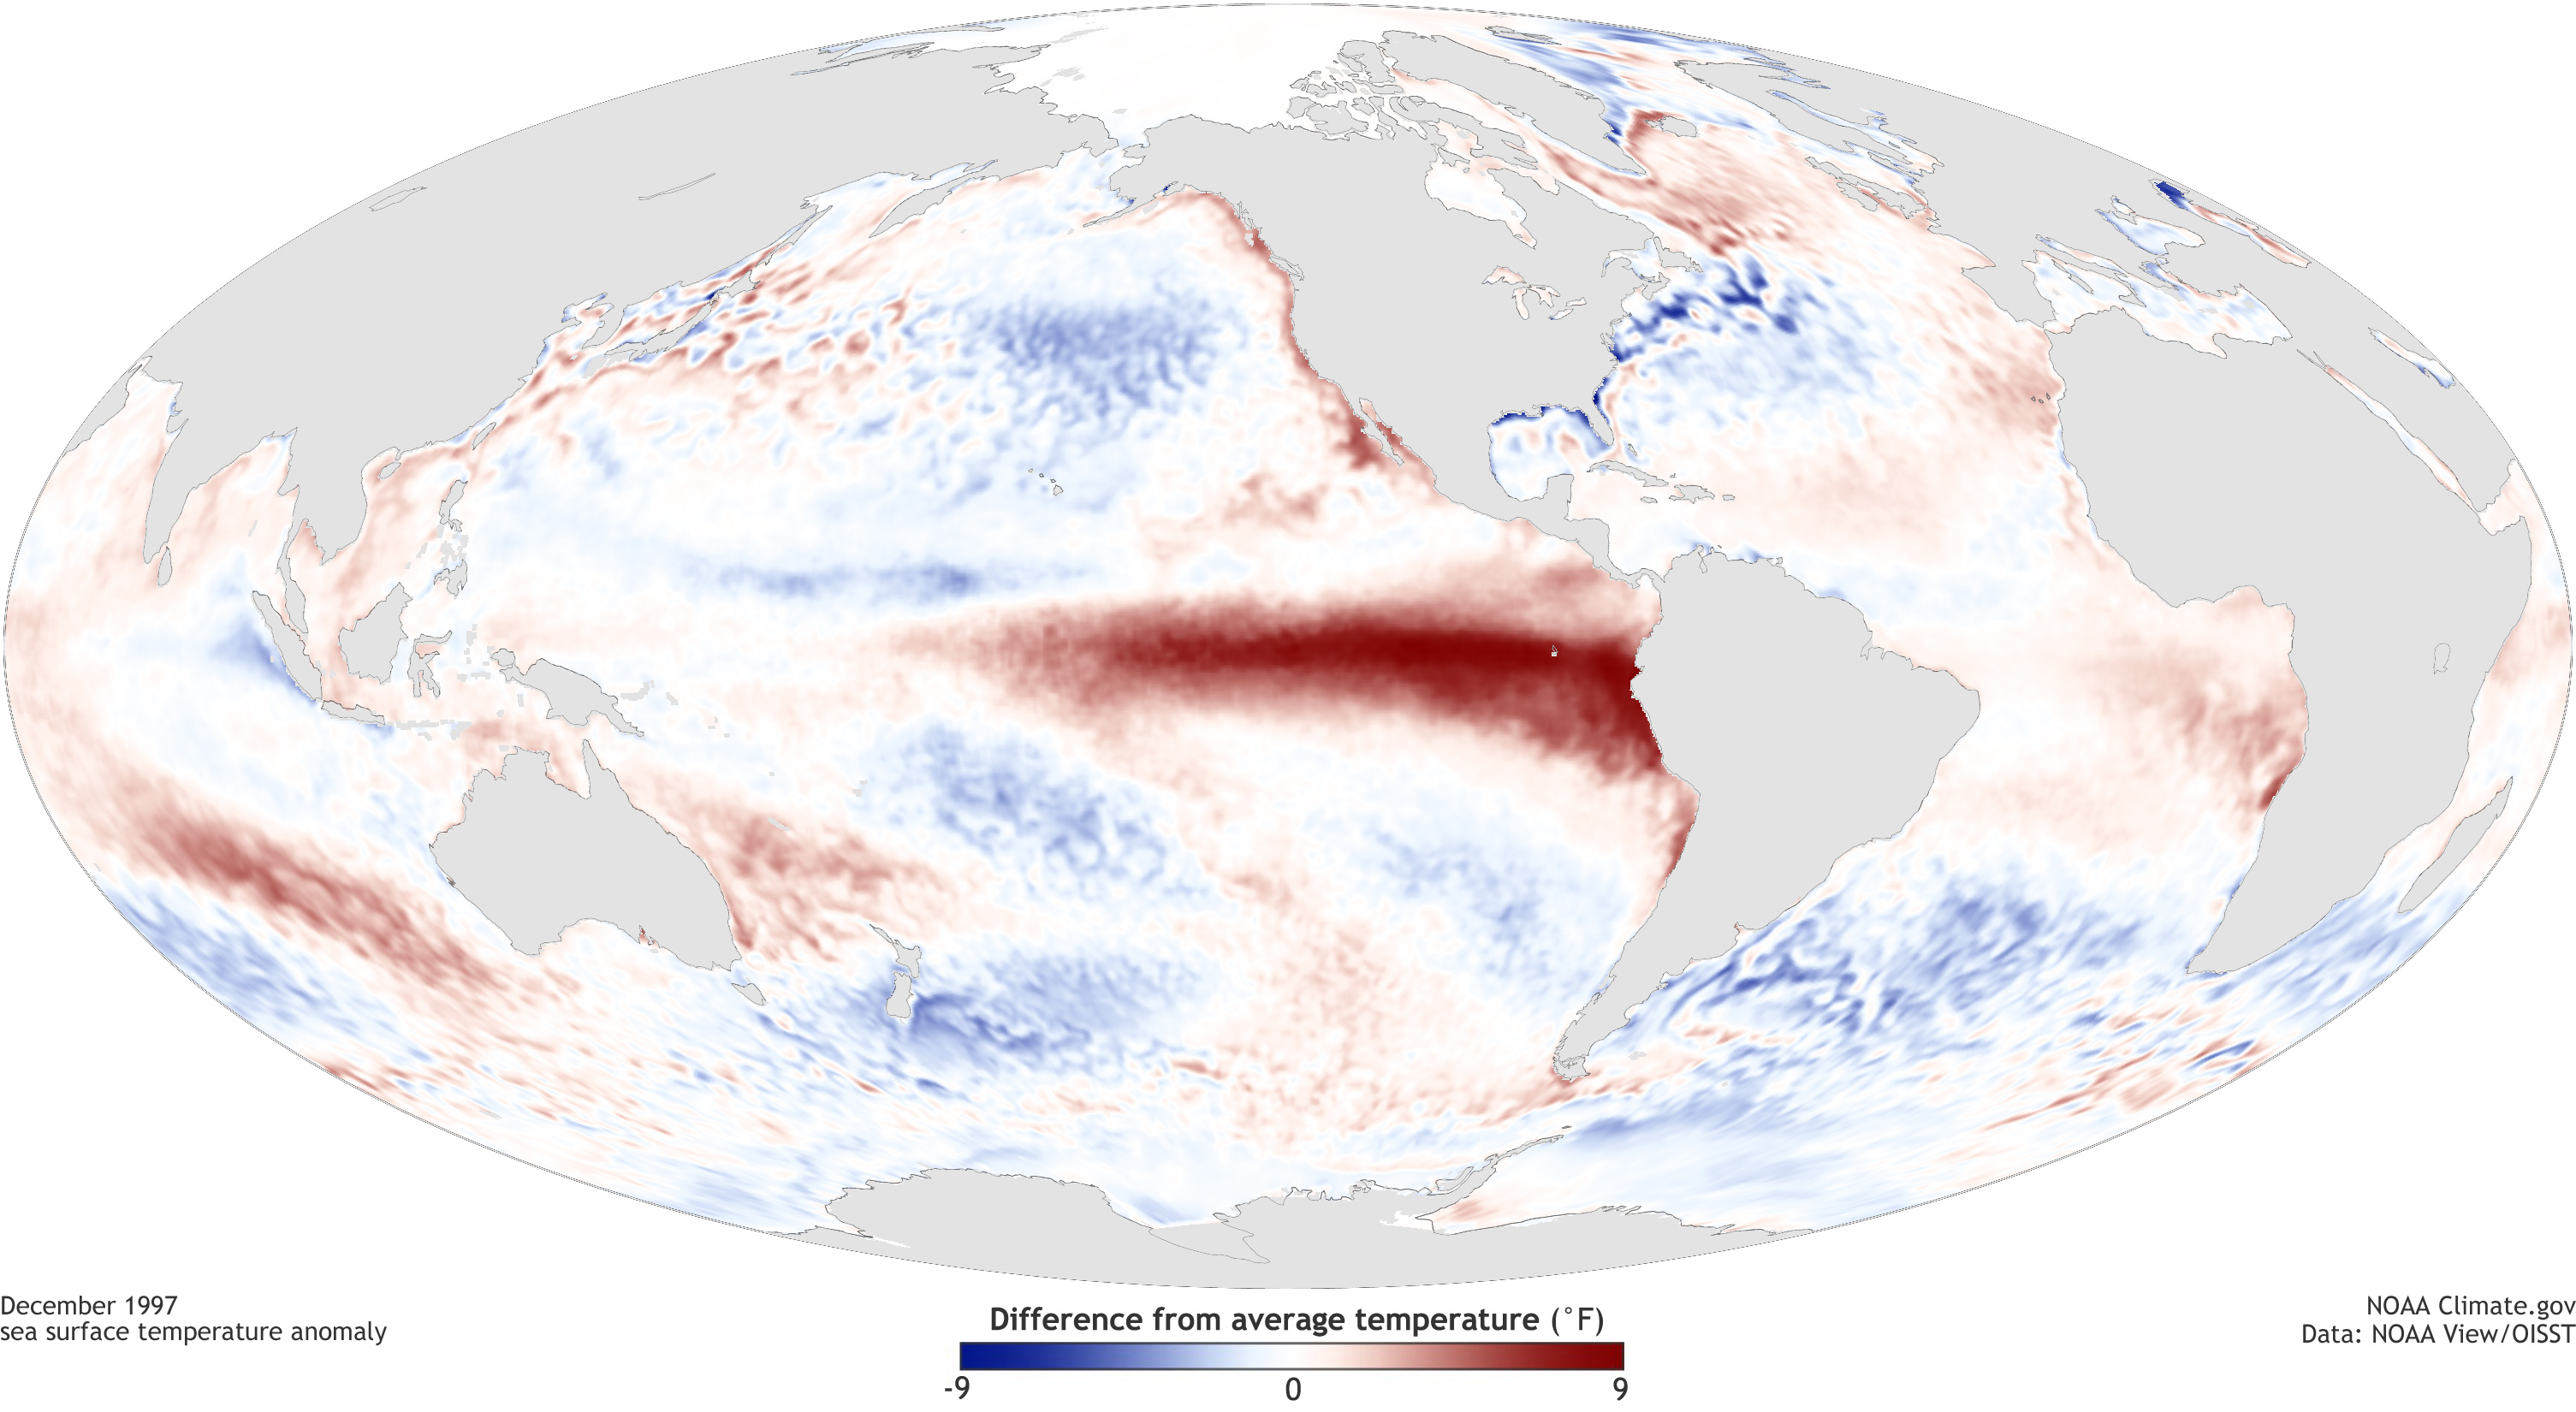
\includegraphics[width=0.7\textwidth]{../images/iconic_ENSO_elNino_lrg.jpg}
        \end{center}
    \end{frame}

    \begin{frame}
        \frametitle{El Niño Southern Oscillation (ENSO)}
        \begin{center}
            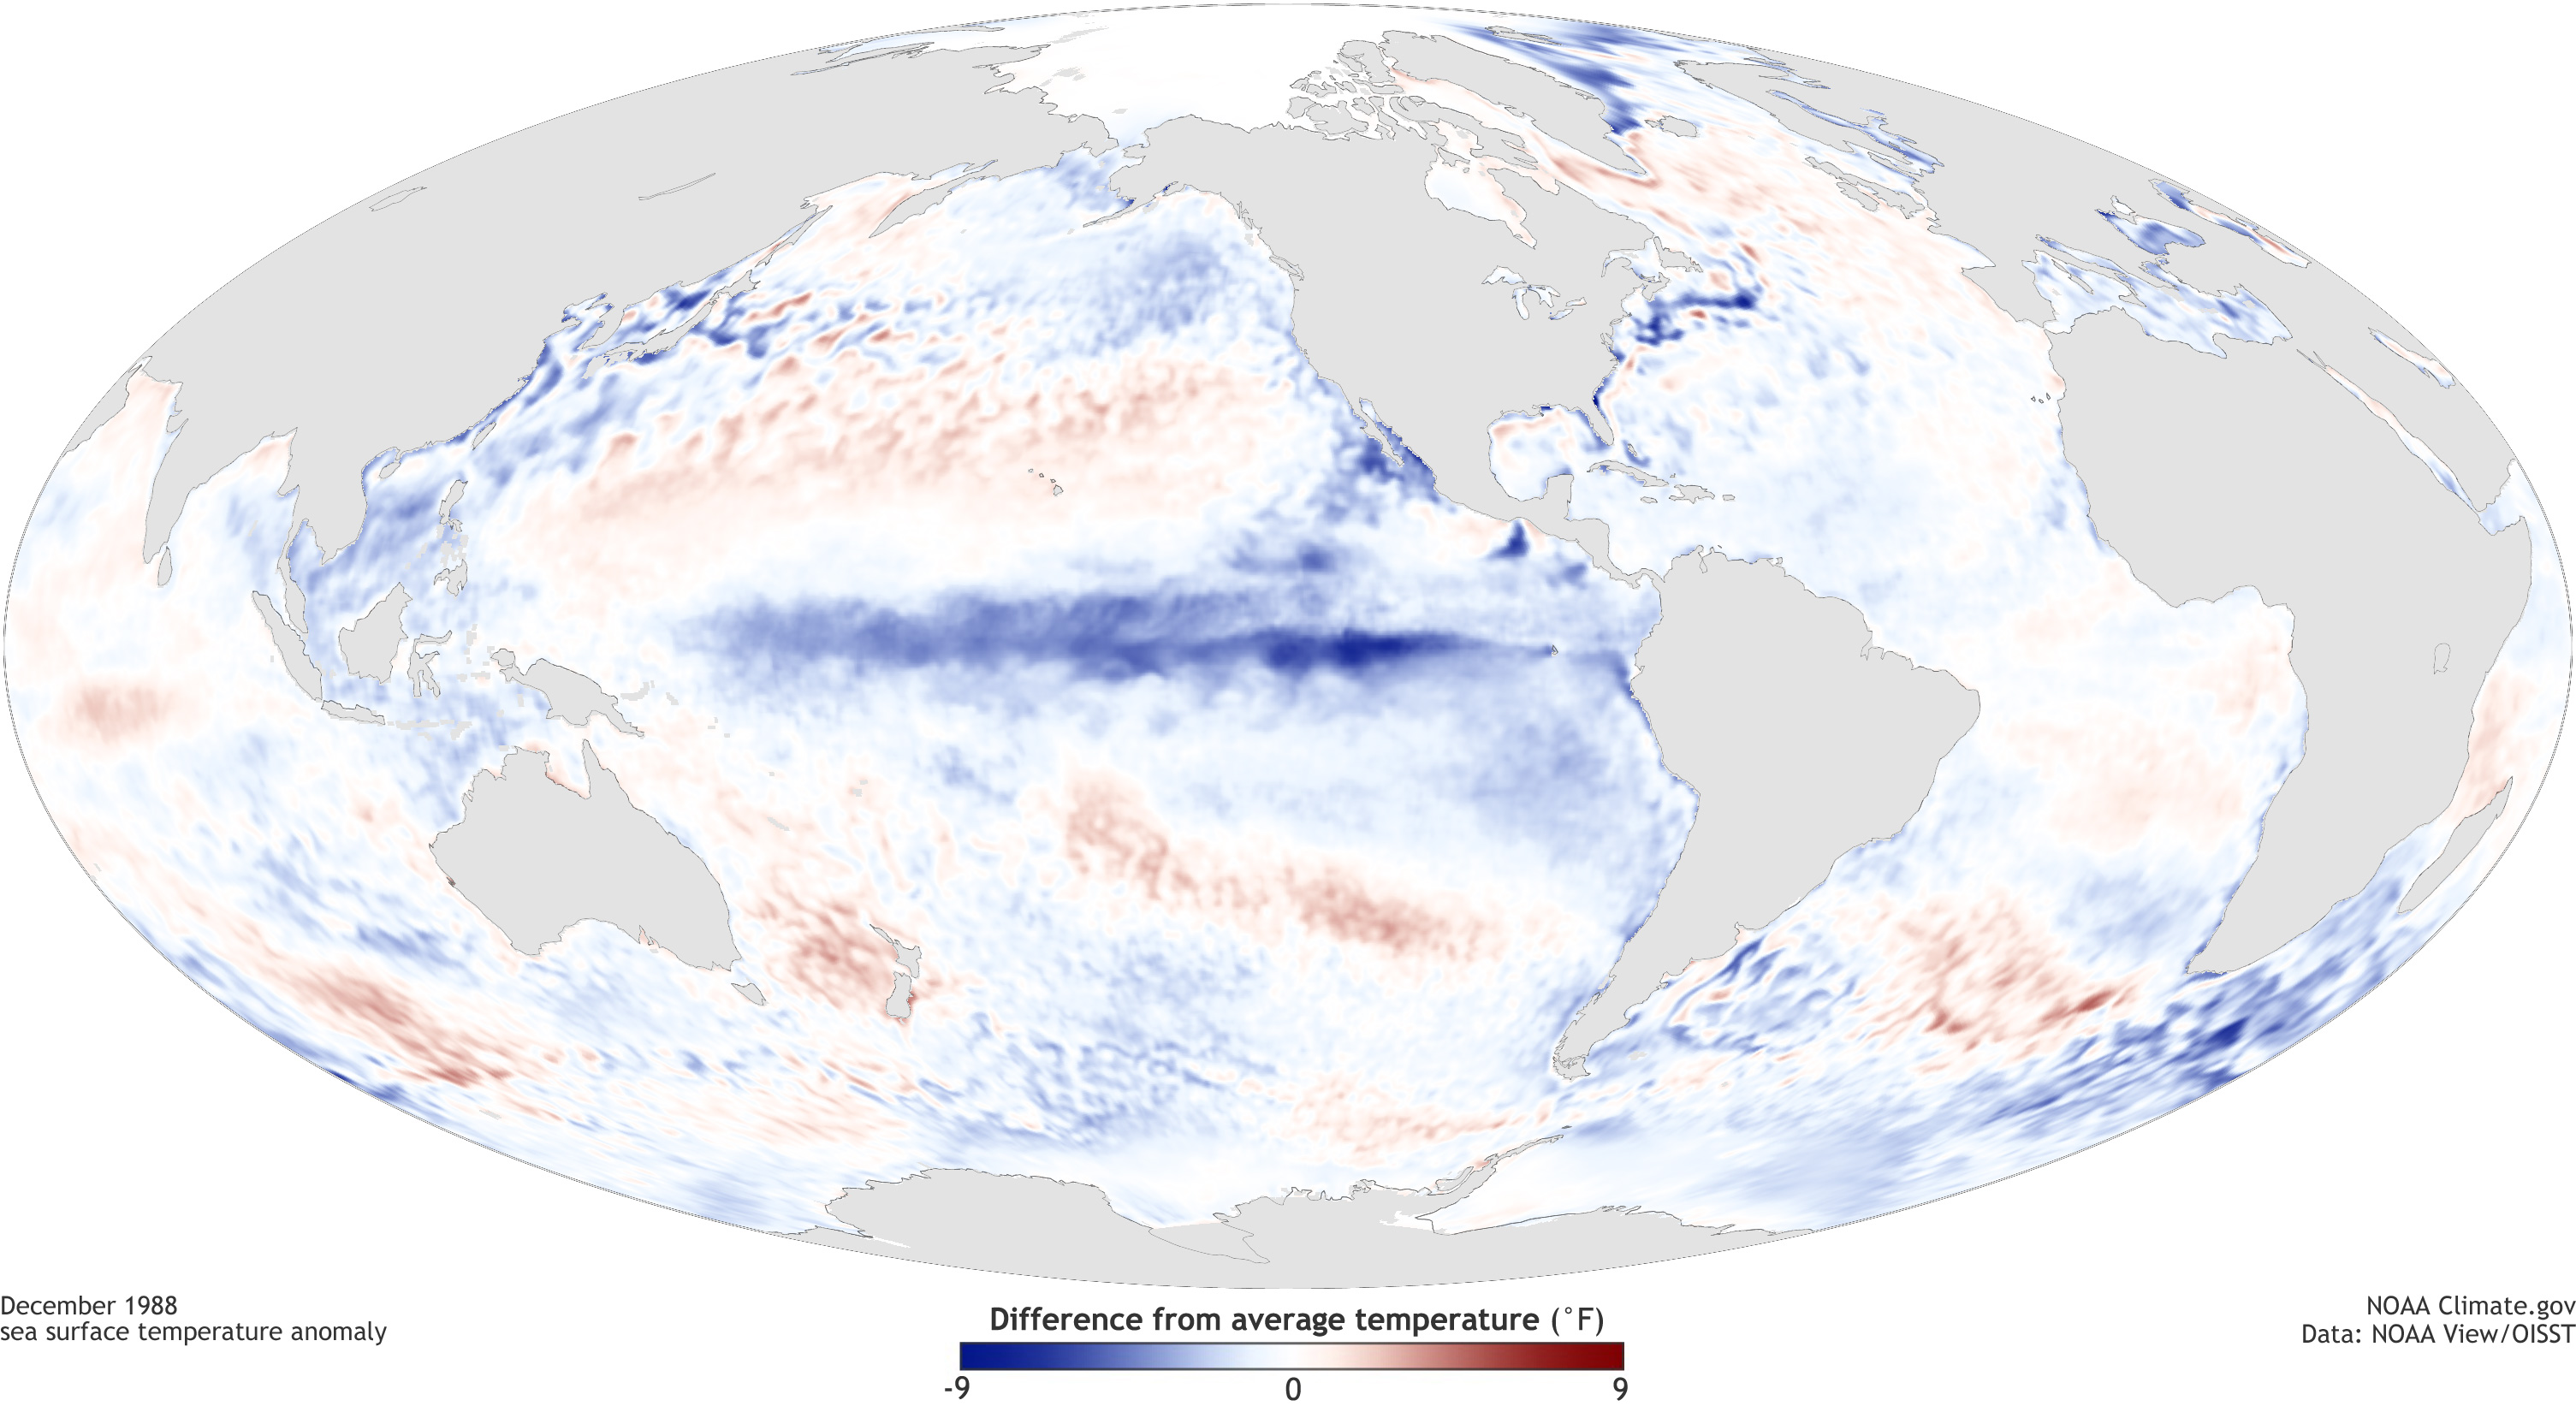
\includegraphics[width=0.7\textwidth]{../images/iconic_ENSO_laNina_lrg.jpg}
        \end{center}
    \end{frame}

    \begin{frame}
        \frametitle{El Niño Southern Oscillation (ENSO)}
        \begin{center}
            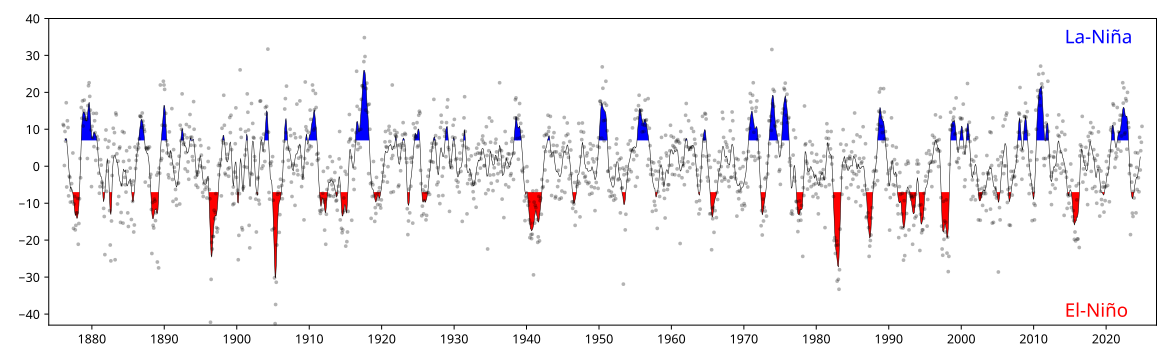
\includegraphics[width=\textwidth]{../images/elnino_data.png}
        \end{center}
    \end{frame}

    \begin{frame}
        \frametitle{Modellierung als dynamisches System}
        Recharge Oscillator Modell:
        \begin{align*}
            \frac{dT_E}{dt} &= -cT_E + \gamma \left(bT_E + h_W\right) - \epsilon \left(bT_E + h_W\right)^3, \\
            \frac{dh_W}{dt} &= -rh_W - \alpha b T_E.
        \end{align*}
        \pause
        Vereinfachen:
        \begin{align*}
            \dot{x} &= -x + \gamma \left(bx + y\right) - \epsilon \left(bx + y\right)^3, \\
            \dot{y} &= -ry - \alpha b x.
        \end{align*}
    \end{frame}

    \begin{frame}
    \frametitle{Gewünschte Eigenschaften}
        Das Recharge Oscillator ENSO Modell soll folgende Eigenschaften haben:
        \begin{itemize}
            \item Oszillierend
            \item Kleine Änderungen der Parameter ändert nicht viel an der Lösung
            \item Anfangsbedingungen spielen keine grosse Rolle
        \end{itemize}
    \end{frame}

	\section{Poincaré-Bendixson}

    \begin{frame}
    \frametitle{Nullklinen}
        Wir betrachten das System

        \begin{align*}
            \dot{x} &= y - x^2 \\
            \dot{y} &= x - 2
        \end{align*}
        \pause
        $x$-Nullkline:
        \begin{equation*}
            y = x^2
        \end{equation*}
        \pause
        $y$-Nullkline:
        \begin{equation*}
            x = 2
        \end{equation*}
    \end{frame}
    \begin{frame}
    \frametitle{Nullklinen: Unterteilung in Sektoren}
        \begin{center}
            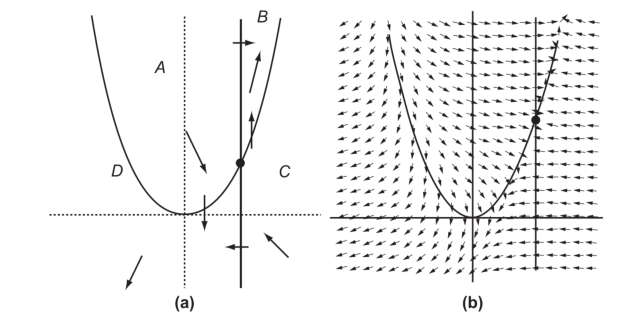
\includegraphics[width=0.7\textwidth]{../images/nullklinen.pdf}
        \end{center}
    \end{frame}

    \begin{frame}
    \frametitle{Limesmengen}
        Dynamisches System $\Phi_t(p)$ hat die Alpha- und Omega-Limesmenge:

        \begin{align*}
            \alpha(p) &= \lim_{t\to-\infty} \Phi_t(p) \\
            \omega(p) &= \lim_{t\to\infty} \Phi_t(p)
        \end{align*}
    \end{frame}
    \begin{frame}
    \frametitle{Poincaré-Bendixson: Fall 1}
        \begin{enumerate}
            \item $\omega(p)$ ist eine Singularität
        \end{enumerate}
        \begin{center}
            %% Creator: Matplotlib, PGF backend
%%
%% To include the figure in your LaTeX document, write
%%   \input{<filename>.pgf}
%%
%% Make sure the required packages are loaded in your preamble
%%   \usepackage{pgf}
%%
%% Also ensure that all the required font packages are loaded; for instance,
%% the lmodern package is sometimes necessary when using math font.
%%   \usepackage{lmodern}
%%
%% Figures using additional raster images can only be included by \input if
%% they are in the same directory as the main LaTeX file. For loading figures
%% from other directories you can use the `import` package
%%   \usepackage{import}
%%
%% and then include the figures with
%%   \import{<path to file>}{<filename>.pgf}
%%
%% Matplotlib used the following preamble
%%   \usepackage{bm}
%%   \usepackage{amsmath}
%%   \usepackage{xcolor}
%%   \usepackage{tgtermes}
%%   \makeatletter\@ifpackageloaded{underscore}{}{\usepackage[strings]{underscore}}\makeatother
%%
\begingroup%
\makeatletter%
\begin{pgfpicture}%
\pgfpathrectangle{\pgfpointorigin}{\pgfqpoint{4.500000in}{2.500000in}}%
\pgfusepath{use as bounding box, clip}%
\begin{pgfscope}%
\pgfsetbuttcap%
\pgfsetmiterjoin%
\definecolor{currentfill}{rgb}{1.000000,1.000000,1.000000}%
\pgfsetfillcolor{currentfill}%
\pgfsetlinewidth{0.000000pt}%
\definecolor{currentstroke}{rgb}{1.000000,1.000000,1.000000}%
\pgfsetstrokecolor{currentstroke}%
\pgfsetdash{}{0pt}%
\pgfpathmoveto{\pgfqpoint{0.000000in}{0.000000in}}%
\pgfpathlineto{\pgfqpoint{4.500000in}{0.000000in}}%
\pgfpathlineto{\pgfqpoint{4.500000in}{2.500000in}}%
\pgfpathlineto{\pgfqpoint{0.000000in}{2.500000in}}%
\pgfpathlineto{\pgfqpoint{0.000000in}{0.000000in}}%
\pgfpathclose%
\pgfusepath{fill}%
\end{pgfscope}%
\begin{pgfscope}%
\pgfsetbuttcap%
\pgfsetmiterjoin%
\definecolor{currentfill}{rgb}{1.000000,1.000000,1.000000}%
\pgfsetfillcolor{currentfill}%
\pgfsetlinewidth{0.000000pt}%
\definecolor{currentstroke}{rgb}{0.000000,0.000000,0.000000}%
\pgfsetstrokecolor{currentstroke}%
\pgfsetstrokeopacity{0.000000}%
\pgfsetdash{}{0pt}%
\pgfpathmoveto{\pgfqpoint{0.562500in}{0.275000in}}%
\pgfpathlineto{\pgfqpoint{4.050000in}{0.275000in}}%
\pgfpathlineto{\pgfqpoint{4.050000in}{2.200000in}}%
\pgfpathlineto{\pgfqpoint{0.562500in}{2.200000in}}%
\pgfpathlineto{\pgfqpoint{0.562500in}{0.275000in}}%
\pgfpathclose%
\pgfusepath{fill}%
\end{pgfscope}%
\begin{pgfscope}%
\pgfpathrectangle{\pgfqpoint{0.562500in}{0.275000in}}{\pgfqpoint{3.487500in}{1.925000in}}%
\pgfusepath{clip}%
\pgfsetrectcap%
\pgfsetroundjoin%
\pgfsetlinewidth{0.803000pt}%
\definecolor{currentstroke}{rgb}{0.690196,0.690196,0.690196}%
\pgfsetstrokecolor{currentstroke}%
\pgfsetdash{}{0pt}%
\pgfpathmoveto{\pgfqpoint{0.732791in}{0.275000in}}%
\pgfpathlineto{\pgfqpoint{0.732791in}{2.200000in}}%
\pgfusepath{stroke}%
\end{pgfscope}%
\begin{pgfscope}%
\pgfsetbuttcap%
\pgfsetroundjoin%
\definecolor{currentfill}{rgb}{0.000000,0.000000,0.000000}%
\pgfsetfillcolor{currentfill}%
\pgfsetlinewidth{0.803000pt}%
\definecolor{currentstroke}{rgb}{0.000000,0.000000,0.000000}%
\pgfsetstrokecolor{currentstroke}%
\pgfsetdash{}{0pt}%
\pgfsys@defobject{currentmarker}{\pgfqpoint{0.000000in}{-0.048611in}}{\pgfqpoint{0.000000in}{0.000000in}}{%
\pgfpathmoveto{\pgfqpoint{0.000000in}{0.000000in}}%
\pgfpathlineto{\pgfqpoint{0.000000in}{-0.048611in}}%
\pgfusepath{stroke,fill}%
}%
\begin{pgfscope}%
\pgfsys@transformshift{0.732791in}{0.275000in}%
\pgfsys@useobject{currentmarker}{}%
\end{pgfscope}%
\end{pgfscope}%
\begin{pgfscope}%
\definecolor{textcolor}{rgb}{0.000000,0.000000,0.000000}%
\pgfsetstrokecolor{textcolor}%
\pgfsetfillcolor{textcolor}%
\pgftext[x=0.732791in,y=0.177778in,,top]{\color{textcolor}\rmfamily\fontsize{10.000000}{12.000000}\selectfont \(\displaystyle {-1.0}\)}%
\end{pgfscope}%
\begin{pgfscope}%
\pgfpathrectangle{\pgfqpoint{0.562500in}{0.275000in}}{\pgfqpoint{3.487500in}{1.925000in}}%
\pgfusepath{clip}%
\pgfsetrectcap%
\pgfsetroundjoin%
\pgfsetlinewidth{0.803000pt}%
\definecolor{currentstroke}{rgb}{0.690196,0.690196,0.690196}%
\pgfsetstrokecolor{currentstroke}%
\pgfsetdash{}{0pt}%
\pgfpathmoveto{\pgfqpoint{1.522463in}{0.275000in}}%
\pgfpathlineto{\pgfqpoint{1.522463in}{2.200000in}}%
\pgfusepath{stroke}%
\end{pgfscope}%
\begin{pgfscope}%
\pgfsetbuttcap%
\pgfsetroundjoin%
\definecolor{currentfill}{rgb}{0.000000,0.000000,0.000000}%
\pgfsetfillcolor{currentfill}%
\pgfsetlinewidth{0.803000pt}%
\definecolor{currentstroke}{rgb}{0.000000,0.000000,0.000000}%
\pgfsetstrokecolor{currentstroke}%
\pgfsetdash{}{0pt}%
\pgfsys@defobject{currentmarker}{\pgfqpoint{0.000000in}{-0.048611in}}{\pgfqpoint{0.000000in}{0.000000in}}{%
\pgfpathmoveto{\pgfqpoint{0.000000in}{0.000000in}}%
\pgfpathlineto{\pgfqpoint{0.000000in}{-0.048611in}}%
\pgfusepath{stroke,fill}%
}%
\begin{pgfscope}%
\pgfsys@transformshift{1.522463in}{0.275000in}%
\pgfsys@useobject{currentmarker}{}%
\end{pgfscope}%
\end{pgfscope}%
\begin{pgfscope}%
\definecolor{textcolor}{rgb}{0.000000,0.000000,0.000000}%
\pgfsetstrokecolor{textcolor}%
\pgfsetfillcolor{textcolor}%
\pgftext[x=1.522463in,y=0.177778in,,top]{\color{textcolor}\rmfamily\fontsize{10.000000}{12.000000}\selectfont \(\displaystyle {-0.5}\)}%
\end{pgfscope}%
\begin{pgfscope}%
\pgfpathrectangle{\pgfqpoint{0.562500in}{0.275000in}}{\pgfqpoint{3.487500in}{1.925000in}}%
\pgfusepath{clip}%
\pgfsetrectcap%
\pgfsetroundjoin%
\pgfsetlinewidth{0.803000pt}%
\definecolor{currentstroke}{rgb}{0.690196,0.690196,0.690196}%
\pgfsetstrokecolor{currentstroke}%
\pgfsetdash{}{0pt}%
\pgfpathmoveto{\pgfqpoint{2.312134in}{0.275000in}}%
\pgfpathlineto{\pgfqpoint{2.312134in}{2.200000in}}%
\pgfusepath{stroke}%
\end{pgfscope}%
\begin{pgfscope}%
\pgfsetbuttcap%
\pgfsetroundjoin%
\definecolor{currentfill}{rgb}{0.000000,0.000000,0.000000}%
\pgfsetfillcolor{currentfill}%
\pgfsetlinewidth{0.803000pt}%
\definecolor{currentstroke}{rgb}{0.000000,0.000000,0.000000}%
\pgfsetstrokecolor{currentstroke}%
\pgfsetdash{}{0pt}%
\pgfsys@defobject{currentmarker}{\pgfqpoint{0.000000in}{-0.048611in}}{\pgfqpoint{0.000000in}{0.000000in}}{%
\pgfpathmoveto{\pgfqpoint{0.000000in}{0.000000in}}%
\pgfpathlineto{\pgfqpoint{0.000000in}{-0.048611in}}%
\pgfusepath{stroke,fill}%
}%
\begin{pgfscope}%
\pgfsys@transformshift{2.312134in}{0.275000in}%
\pgfsys@useobject{currentmarker}{}%
\end{pgfscope}%
\end{pgfscope}%
\begin{pgfscope}%
\definecolor{textcolor}{rgb}{0.000000,0.000000,0.000000}%
\pgfsetstrokecolor{textcolor}%
\pgfsetfillcolor{textcolor}%
\pgftext[x=2.312134in,y=0.177778in,,top]{\color{textcolor}\rmfamily\fontsize{10.000000}{12.000000}\selectfont \(\displaystyle {0.0}\)}%
\end{pgfscope}%
\begin{pgfscope}%
\pgfpathrectangle{\pgfqpoint{0.562500in}{0.275000in}}{\pgfqpoint{3.487500in}{1.925000in}}%
\pgfusepath{clip}%
\pgfsetrectcap%
\pgfsetroundjoin%
\pgfsetlinewidth{0.803000pt}%
\definecolor{currentstroke}{rgb}{0.690196,0.690196,0.690196}%
\pgfsetstrokecolor{currentstroke}%
\pgfsetdash{}{0pt}%
\pgfpathmoveto{\pgfqpoint{3.101806in}{0.275000in}}%
\pgfpathlineto{\pgfqpoint{3.101806in}{2.200000in}}%
\pgfusepath{stroke}%
\end{pgfscope}%
\begin{pgfscope}%
\pgfsetbuttcap%
\pgfsetroundjoin%
\definecolor{currentfill}{rgb}{0.000000,0.000000,0.000000}%
\pgfsetfillcolor{currentfill}%
\pgfsetlinewidth{0.803000pt}%
\definecolor{currentstroke}{rgb}{0.000000,0.000000,0.000000}%
\pgfsetstrokecolor{currentstroke}%
\pgfsetdash{}{0pt}%
\pgfsys@defobject{currentmarker}{\pgfqpoint{0.000000in}{-0.048611in}}{\pgfqpoint{0.000000in}{0.000000in}}{%
\pgfpathmoveto{\pgfqpoint{0.000000in}{0.000000in}}%
\pgfpathlineto{\pgfqpoint{0.000000in}{-0.048611in}}%
\pgfusepath{stroke,fill}%
}%
\begin{pgfscope}%
\pgfsys@transformshift{3.101806in}{0.275000in}%
\pgfsys@useobject{currentmarker}{}%
\end{pgfscope}%
\end{pgfscope}%
\begin{pgfscope}%
\definecolor{textcolor}{rgb}{0.000000,0.000000,0.000000}%
\pgfsetstrokecolor{textcolor}%
\pgfsetfillcolor{textcolor}%
\pgftext[x=3.101806in,y=0.177778in,,top]{\color{textcolor}\rmfamily\fontsize{10.000000}{12.000000}\selectfont \(\displaystyle {0.5}\)}%
\end{pgfscope}%
\begin{pgfscope}%
\pgfpathrectangle{\pgfqpoint{0.562500in}{0.275000in}}{\pgfqpoint{3.487500in}{1.925000in}}%
\pgfusepath{clip}%
\pgfsetrectcap%
\pgfsetroundjoin%
\pgfsetlinewidth{0.803000pt}%
\definecolor{currentstroke}{rgb}{0.690196,0.690196,0.690196}%
\pgfsetstrokecolor{currentstroke}%
\pgfsetdash{}{0pt}%
\pgfpathmoveto{\pgfqpoint{3.891477in}{0.275000in}}%
\pgfpathlineto{\pgfqpoint{3.891477in}{2.200000in}}%
\pgfusepath{stroke}%
\end{pgfscope}%
\begin{pgfscope}%
\pgfsetbuttcap%
\pgfsetroundjoin%
\definecolor{currentfill}{rgb}{0.000000,0.000000,0.000000}%
\pgfsetfillcolor{currentfill}%
\pgfsetlinewidth{0.803000pt}%
\definecolor{currentstroke}{rgb}{0.000000,0.000000,0.000000}%
\pgfsetstrokecolor{currentstroke}%
\pgfsetdash{}{0pt}%
\pgfsys@defobject{currentmarker}{\pgfqpoint{0.000000in}{-0.048611in}}{\pgfqpoint{0.000000in}{0.000000in}}{%
\pgfpathmoveto{\pgfqpoint{0.000000in}{0.000000in}}%
\pgfpathlineto{\pgfqpoint{0.000000in}{-0.048611in}}%
\pgfusepath{stroke,fill}%
}%
\begin{pgfscope}%
\pgfsys@transformshift{3.891477in}{0.275000in}%
\pgfsys@useobject{currentmarker}{}%
\end{pgfscope}%
\end{pgfscope}%
\begin{pgfscope}%
\definecolor{textcolor}{rgb}{0.000000,0.000000,0.000000}%
\pgfsetstrokecolor{textcolor}%
\pgfsetfillcolor{textcolor}%
\pgftext[x=3.891477in,y=0.177778in,,top]{\color{textcolor}\rmfamily\fontsize{10.000000}{12.000000}\selectfont \(\displaystyle {1.0}\)}%
\end{pgfscope}%
\begin{pgfscope}%
\pgfpathrectangle{\pgfqpoint{0.562500in}{0.275000in}}{\pgfqpoint{3.487500in}{1.925000in}}%
\pgfusepath{clip}%
\pgfsetrectcap%
\pgfsetroundjoin%
\pgfsetlinewidth{0.803000pt}%
\definecolor{currentstroke}{rgb}{0.690196,0.690196,0.690196}%
\pgfsetstrokecolor{currentstroke}%
\pgfsetdash{}{0pt}%
\pgfpathmoveto{\pgfqpoint{0.562500in}{0.362500in}}%
\pgfpathlineto{\pgfqpoint{4.050000in}{0.362500in}}%
\pgfusepath{stroke}%
\end{pgfscope}%
\begin{pgfscope}%
\pgfsetbuttcap%
\pgfsetroundjoin%
\definecolor{currentfill}{rgb}{0.000000,0.000000,0.000000}%
\pgfsetfillcolor{currentfill}%
\pgfsetlinewidth{0.803000pt}%
\definecolor{currentstroke}{rgb}{0.000000,0.000000,0.000000}%
\pgfsetstrokecolor{currentstroke}%
\pgfsetdash{}{0pt}%
\pgfsys@defobject{currentmarker}{\pgfqpoint{-0.048611in}{0.000000in}}{\pgfqpoint{-0.000000in}{0.000000in}}{%
\pgfpathmoveto{\pgfqpoint{-0.000000in}{0.000000in}}%
\pgfpathlineto{\pgfqpoint{-0.048611in}{0.000000in}}%
\pgfusepath{stroke,fill}%
}%
\begin{pgfscope}%
\pgfsys@transformshift{0.562500in}{0.362500in}%
\pgfsys@useobject{currentmarker}{}%
\end{pgfscope}%
\end{pgfscope}%
\begin{pgfscope}%
\definecolor{textcolor}{rgb}{0.000000,0.000000,0.000000}%
\pgfsetstrokecolor{textcolor}%
\pgfsetfillcolor{textcolor}%
\pgftext[x=0.287808in, y=0.315799in, left, base]{\color{textcolor}\rmfamily\fontsize{10.000000}{12.000000}\selectfont \(\displaystyle {-1}\)}%
\end{pgfscope}%
\begin{pgfscope}%
\pgfpathrectangle{\pgfqpoint{0.562500in}{0.275000in}}{\pgfqpoint{3.487500in}{1.925000in}}%
\pgfusepath{clip}%
\pgfsetrectcap%
\pgfsetroundjoin%
\pgfsetlinewidth{0.803000pt}%
\definecolor{currentstroke}{rgb}{0.690196,0.690196,0.690196}%
\pgfsetstrokecolor{currentstroke}%
\pgfsetdash{}{0pt}%
\pgfpathmoveto{\pgfqpoint{0.562500in}{0.943734in}}%
\pgfpathlineto{\pgfqpoint{4.050000in}{0.943734in}}%
\pgfusepath{stroke}%
\end{pgfscope}%
\begin{pgfscope}%
\pgfsetbuttcap%
\pgfsetroundjoin%
\definecolor{currentfill}{rgb}{0.000000,0.000000,0.000000}%
\pgfsetfillcolor{currentfill}%
\pgfsetlinewidth{0.803000pt}%
\definecolor{currentstroke}{rgb}{0.000000,0.000000,0.000000}%
\pgfsetstrokecolor{currentstroke}%
\pgfsetdash{}{0pt}%
\pgfsys@defobject{currentmarker}{\pgfqpoint{-0.048611in}{0.000000in}}{\pgfqpoint{-0.000000in}{0.000000in}}{%
\pgfpathmoveto{\pgfqpoint{-0.000000in}{0.000000in}}%
\pgfpathlineto{\pgfqpoint{-0.048611in}{0.000000in}}%
\pgfusepath{stroke,fill}%
}%
\begin{pgfscope}%
\pgfsys@transformshift{0.562500in}{0.943734in}%
\pgfsys@useobject{currentmarker}{}%
\end{pgfscope}%
\end{pgfscope}%
\begin{pgfscope}%
\definecolor{textcolor}{rgb}{0.000000,0.000000,0.000000}%
\pgfsetstrokecolor{textcolor}%
\pgfsetfillcolor{textcolor}%
\pgftext[x=0.395833in, y=0.897032in, left, base]{\color{textcolor}\rmfamily\fontsize{10.000000}{12.000000}\selectfont \(\displaystyle {0}\)}%
\end{pgfscope}%
\begin{pgfscope}%
\pgfpathrectangle{\pgfqpoint{0.562500in}{0.275000in}}{\pgfqpoint{3.487500in}{1.925000in}}%
\pgfusepath{clip}%
\pgfsetrectcap%
\pgfsetroundjoin%
\pgfsetlinewidth{0.803000pt}%
\definecolor{currentstroke}{rgb}{0.690196,0.690196,0.690196}%
\pgfsetstrokecolor{currentstroke}%
\pgfsetdash{}{0pt}%
\pgfpathmoveto{\pgfqpoint{0.562500in}{1.524967in}}%
\pgfpathlineto{\pgfqpoint{4.050000in}{1.524967in}}%
\pgfusepath{stroke}%
\end{pgfscope}%
\begin{pgfscope}%
\pgfsetbuttcap%
\pgfsetroundjoin%
\definecolor{currentfill}{rgb}{0.000000,0.000000,0.000000}%
\pgfsetfillcolor{currentfill}%
\pgfsetlinewidth{0.803000pt}%
\definecolor{currentstroke}{rgb}{0.000000,0.000000,0.000000}%
\pgfsetstrokecolor{currentstroke}%
\pgfsetdash{}{0pt}%
\pgfsys@defobject{currentmarker}{\pgfqpoint{-0.048611in}{0.000000in}}{\pgfqpoint{-0.000000in}{0.000000in}}{%
\pgfpathmoveto{\pgfqpoint{-0.000000in}{0.000000in}}%
\pgfpathlineto{\pgfqpoint{-0.048611in}{0.000000in}}%
\pgfusepath{stroke,fill}%
}%
\begin{pgfscope}%
\pgfsys@transformshift{0.562500in}{1.524967in}%
\pgfsys@useobject{currentmarker}{}%
\end{pgfscope}%
\end{pgfscope}%
\begin{pgfscope}%
\definecolor{textcolor}{rgb}{0.000000,0.000000,0.000000}%
\pgfsetstrokecolor{textcolor}%
\pgfsetfillcolor{textcolor}%
\pgftext[x=0.395833in, y=1.478266in, left, base]{\color{textcolor}\rmfamily\fontsize{10.000000}{12.000000}\selectfont \(\displaystyle {1}\)}%
\end{pgfscope}%
\begin{pgfscope}%
\pgfpathrectangle{\pgfqpoint{0.562500in}{0.275000in}}{\pgfqpoint{3.487500in}{1.925000in}}%
\pgfusepath{clip}%
\pgfsetrectcap%
\pgfsetroundjoin%
\pgfsetlinewidth{0.803000pt}%
\definecolor{currentstroke}{rgb}{0.690196,0.690196,0.690196}%
\pgfsetstrokecolor{currentstroke}%
\pgfsetdash{}{0pt}%
\pgfpathmoveto{\pgfqpoint{0.562500in}{2.106201in}}%
\pgfpathlineto{\pgfqpoint{4.050000in}{2.106201in}}%
\pgfusepath{stroke}%
\end{pgfscope}%
\begin{pgfscope}%
\pgfsetbuttcap%
\pgfsetroundjoin%
\definecolor{currentfill}{rgb}{0.000000,0.000000,0.000000}%
\pgfsetfillcolor{currentfill}%
\pgfsetlinewidth{0.803000pt}%
\definecolor{currentstroke}{rgb}{0.000000,0.000000,0.000000}%
\pgfsetstrokecolor{currentstroke}%
\pgfsetdash{}{0pt}%
\pgfsys@defobject{currentmarker}{\pgfqpoint{-0.048611in}{0.000000in}}{\pgfqpoint{-0.000000in}{0.000000in}}{%
\pgfpathmoveto{\pgfqpoint{-0.000000in}{0.000000in}}%
\pgfpathlineto{\pgfqpoint{-0.048611in}{0.000000in}}%
\pgfusepath{stroke,fill}%
}%
\begin{pgfscope}%
\pgfsys@transformshift{0.562500in}{2.106201in}%
\pgfsys@useobject{currentmarker}{}%
\end{pgfscope}%
\end{pgfscope}%
\begin{pgfscope}%
\definecolor{textcolor}{rgb}{0.000000,0.000000,0.000000}%
\pgfsetstrokecolor{textcolor}%
\pgfsetfillcolor{textcolor}%
\pgftext[x=0.395833in, y=2.059500in, left, base]{\color{textcolor}\rmfamily\fontsize{10.000000}{12.000000}\selectfont \(\displaystyle {2}\)}%
\end{pgfscope}%
\begin{pgfscope}%
\pgfpathrectangle{\pgfqpoint{0.562500in}{0.275000in}}{\pgfqpoint{3.487500in}{1.925000in}}%
\pgfusepath{clip}%
\pgfsetbuttcap%
\pgfsetroundjoin%
\definecolor{currentfill}{rgb}{0.121569,0.466667,0.705882}%
\pgfsetfillcolor{currentfill}%
\pgfsetlinewidth{1.003750pt}%
\definecolor{currentstroke}{rgb}{0.121569,0.466667,0.705882}%
\pgfsetstrokecolor{currentstroke}%
\pgfsetdash{}{0pt}%
\pgfsys@defobject{currentmarker}{\pgfqpoint{-0.020833in}{-0.020833in}}{\pgfqpoint{0.020833in}{0.020833in}}{%
\pgfpathmoveto{\pgfqpoint{0.000000in}{-0.020833in}}%
\pgfpathcurveto{\pgfqpoint{0.005525in}{-0.020833in}}{\pgfqpoint{0.010825in}{-0.018638in}}{\pgfqpoint{0.014731in}{-0.014731in}}%
\pgfpathcurveto{\pgfqpoint{0.018638in}{-0.010825in}}{\pgfqpoint{0.020833in}{-0.005525in}}{\pgfqpoint{0.020833in}{0.000000in}}%
\pgfpathcurveto{\pgfqpoint{0.020833in}{0.005525in}}{\pgfqpoint{0.018638in}{0.010825in}}{\pgfqpoint{0.014731in}{0.014731in}}%
\pgfpathcurveto{\pgfqpoint{0.010825in}{0.018638in}}{\pgfqpoint{0.005525in}{0.020833in}}{\pgfqpoint{0.000000in}{0.020833in}}%
\pgfpathcurveto{\pgfqpoint{-0.005525in}{0.020833in}}{\pgfqpoint{-0.010825in}{0.018638in}}{\pgfqpoint{-0.014731in}{0.014731in}}%
\pgfpathcurveto{\pgfqpoint{-0.018638in}{0.010825in}}{\pgfqpoint{-0.020833in}{0.005525in}}{\pgfqpoint{-0.020833in}{0.000000in}}%
\pgfpathcurveto{\pgfqpoint{-0.020833in}{-0.005525in}}{\pgfqpoint{-0.018638in}{-0.010825in}}{\pgfqpoint{-0.014731in}{-0.014731in}}%
\pgfpathcurveto{\pgfqpoint{-0.010825in}{-0.018638in}}{\pgfqpoint{-0.005525in}{-0.020833in}}{\pgfqpoint{0.000000in}{-0.020833in}}%
\pgfpathlineto{\pgfqpoint{0.000000in}{-0.020833in}}%
\pgfpathclose%
\pgfusepath{stroke,fill}%
}%
\begin{pgfscope}%
\pgfsys@transformshift{2.312134in}{0.943734in}%
\pgfsys@useobject{currentmarker}{}%
\end{pgfscope}%
\begin{pgfscope}%
\pgfsys@transformshift{2.312134in}{0.943734in}%
\pgfsys@useobject{currentmarker}{}%
\end{pgfscope}%
\begin{pgfscope}%
\pgfsys@transformshift{2.312134in}{0.943734in}%
\pgfsys@useobject{currentmarker}{}%
\end{pgfscope}%
\begin{pgfscope}%
\pgfsys@transformshift{2.312134in}{0.943734in}%
\pgfsys@useobject{currentmarker}{}%
\end{pgfscope}%
\begin{pgfscope}%
\pgfsys@transformshift{2.312134in}{0.943734in}%
\pgfsys@useobject{currentmarker}{}%
\end{pgfscope}%
\begin{pgfscope}%
\pgfsys@transformshift{2.312134in}{0.943734in}%
\pgfsys@useobject{currentmarker}{}%
\end{pgfscope}%
\begin{pgfscope}%
\pgfsys@transformshift{2.312134in}{0.943734in}%
\pgfsys@useobject{currentmarker}{}%
\end{pgfscope}%
\begin{pgfscope}%
\pgfsys@transformshift{2.312134in}{0.943734in}%
\pgfsys@useobject{currentmarker}{}%
\end{pgfscope}%
\begin{pgfscope}%
\pgfsys@transformshift{2.312134in}{0.943734in}%
\pgfsys@useobject{currentmarker}{}%
\end{pgfscope}%
\begin{pgfscope}%
\pgfsys@transformshift{2.312134in}{0.943734in}%
\pgfsys@useobject{currentmarker}{}%
\end{pgfscope}%
\begin{pgfscope}%
\pgfsys@transformshift{2.312134in}{0.943734in}%
\pgfsys@useobject{currentmarker}{}%
\end{pgfscope}%
\begin{pgfscope}%
\pgfsys@transformshift{2.312134in}{0.943734in}%
\pgfsys@useobject{currentmarker}{}%
\end{pgfscope}%
\begin{pgfscope}%
\pgfsys@transformshift{2.312134in}{0.943734in}%
\pgfsys@useobject{currentmarker}{}%
\end{pgfscope}%
\begin{pgfscope}%
\pgfsys@transformshift{2.312134in}{0.943734in}%
\pgfsys@useobject{currentmarker}{}%
\end{pgfscope}%
\begin{pgfscope}%
\pgfsys@transformshift{2.312134in}{0.943734in}%
\pgfsys@useobject{currentmarker}{}%
\end{pgfscope}%
\begin{pgfscope}%
\pgfsys@transformshift{2.312134in}{0.943734in}%
\pgfsys@useobject{currentmarker}{}%
\end{pgfscope}%
\begin{pgfscope}%
\pgfsys@transformshift{2.312134in}{0.943734in}%
\pgfsys@useobject{currentmarker}{}%
\end{pgfscope}%
\begin{pgfscope}%
\pgfsys@transformshift{2.312134in}{0.943734in}%
\pgfsys@useobject{currentmarker}{}%
\end{pgfscope}%
\begin{pgfscope}%
\pgfsys@transformshift{2.312134in}{0.943734in}%
\pgfsys@useobject{currentmarker}{}%
\end{pgfscope}%
\begin{pgfscope}%
\pgfsys@transformshift{2.312134in}{0.943734in}%
\pgfsys@useobject{currentmarker}{}%
\end{pgfscope}%
\begin{pgfscope}%
\pgfsys@transformshift{2.312134in}{0.943734in}%
\pgfsys@useobject{currentmarker}{}%
\end{pgfscope}%
\begin{pgfscope}%
\pgfsys@transformshift{2.312134in}{0.943734in}%
\pgfsys@useobject{currentmarker}{}%
\end{pgfscope}%
\begin{pgfscope}%
\pgfsys@transformshift{2.312134in}{0.943734in}%
\pgfsys@useobject{currentmarker}{}%
\end{pgfscope}%
\begin{pgfscope}%
\pgfsys@transformshift{2.312134in}{0.943734in}%
\pgfsys@useobject{currentmarker}{}%
\end{pgfscope}%
\begin{pgfscope}%
\pgfsys@transformshift{2.312134in}{0.943734in}%
\pgfsys@useobject{currentmarker}{}%
\end{pgfscope}%
\begin{pgfscope}%
\pgfsys@transformshift{2.312134in}{0.943734in}%
\pgfsys@useobject{currentmarker}{}%
\end{pgfscope}%
\begin{pgfscope}%
\pgfsys@transformshift{2.312134in}{0.943734in}%
\pgfsys@useobject{currentmarker}{}%
\end{pgfscope}%
\begin{pgfscope}%
\pgfsys@transformshift{2.312134in}{0.943734in}%
\pgfsys@useobject{currentmarker}{}%
\end{pgfscope}%
\begin{pgfscope}%
\pgfsys@transformshift{2.312134in}{0.943734in}%
\pgfsys@useobject{currentmarker}{}%
\end{pgfscope}%
\begin{pgfscope}%
\pgfsys@transformshift{2.312134in}{0.943734in}%
\pgfsys@useobject{currentmarker}{}%
\end{pgfscope}%
\begin{pgfscope}%
\pgfsys@transformshift{2.312134in}{0.943734in}%
\pgfsys@useobject{currentmarker}{}%
\end{pgfscope}%
\begin{pgfscope}%
\pgfsys@transformshift{2.312134in}{0.943734in}%
\pgfsys@useobject{currentmarker}{}%
\end{pgfscope}%
\begin{pgfscope}%
\pgfsys@transformshift{2.312134in}{0.943734in}%
\pgfsys@useobject{currentmarker}{}%
\end{pgfscope}%
\begin{pgfscope}%
\pgfsys@transformshift{2.312134in}{0.943734in}%
\pgfsys@useobject{currentmarker}{}%
\end{pgfscope}%
\begin{pgfscope}%
\pgfsys@transformshift{2.312134in}{0.943734in}%
\pgfsys@useobject{currentmarker}{}%
\end{pgfscope}%
\begin{pgfscope}%
\pgfsys@transformshift{2.312134in}{0.943734in}%
\pgfsys@useobject{currentmarker}{}%
\end{pgfscope}%
\begin{pgfscope}%
\pgfsys@transformshift{2.312134in}{0.943734in}%
\pgfsys@useobject{currentmarker}{}%
\end{pgfscope}%
\begin{pgfscope}%
\pgfsys@transformshift{2.312134in}{0.943734in}%
\pgfsys@useobject{currentmarker}{}%
\end{pgfscope}%
\begin{pgfscope}%
\pgfsys@transformshift{2.312134in}{0.943734in}%
\pgfsys@useobject{currentmarker}{}%
\end{pgfscope}%
\begin{pgfscope}%
\pgfsys@transformshift{2.312134in}{0.943734in}%
\pgfsys@useobject{currentmarker}{}%
\end{pgfscope}%
\begin{pgfscope}%
\pgfsys@transformshift{2.312134in}{0.943734in}%
\pgfsys@useobject{currentmarker}{}%
\end{pgfscope}%
\begin{pgfscope}%
\pgfsys@transformshift{2.312134in}{0.943734in}%
\pgfsys@useobject{currentmarker}{}%
\end{pgfscope}%
\begin{pgfscope}%
\pgfsys@transformshift{2.312134in}{0.943734in}%
\pgfsys@useobject{currentmarker}{}%
\end{pgfscope}%
\begin{pgfscope}%
\pgfsys@transformshift{2.312134in}{0.943734in}%
\pgfsys@useobject{currentmarker}{}%
\end{pgfscope}%
\begin{pgfscope}%
\pgfsys@transformshift{2.312134in}{0.943734in}%
\pgfsys@useobject{currentmarker}{}%
\end{pgfscope}%
\begin{pgfscope}%
\pgfsys@transformshift{2.312134in}{0.943734in}%
\pgfsys@useobject{currentmarker}{}%
\end{pgfscope}%
\begin{pgfscope}%
\pgfsys@transformshift{2.312134in}{0.943734in}%
\pgfsys@useobject{currentmarker}{}%
\end{pgfscope}%
\begin{pgfscope}%
\pgfsys@transformshift{2.312134in}{0.943734in}%
\pgfsys@useobject{currentmarker}{}%
\end{pgfscope}%
\begin{pgfscope}%
\pgfsys@transformshift{2.312134in}{0.943734in}%
\pgfsys@useobject{currentmarker}{}%
\end{pgfscope}%
\begin{pgfscope}%
\pgfsys@transformshift{2.312134in}{0.943734in}%
\pgfsys@useobject{currentmarker}{}%
\end{pgfscope}%
\begin{pgfscope}%
\pgfsys@transformshift{2.312134in}{0.943734in}%
\pgfsys@useobject{currentmarker}{}%
\end{pgfscope}%
\begin{pgfscope}%
\pgfsys@transformshift{2.312134in}{0.943734in}%
\pgfsys@useobject{currentmarker}{}%
\end{pgfscope}%
\begin{pgfscope}%
\pgfsys@transformshift{2.312134in}{0.943734in}%
\pgfsys@useobject{currentmarker}{}%
\end{pgfscope}%
\begin{pgfscope}%
\pgfsys@transformshift{2.312134in}{0.943734in}%
\pgfsys@useobject{currentmarker}{}%
\end{pgfscope}%
\begin{pgfscope}%
\pgfsys@transformshift{2.312134in}{0.943734in}%
\pgfsys@useobject{currentmarker}{}%
\end{pgfscope}%
\begin{pgfscope}%
\pgfsys@transformshift{2.312134in}{0.943734in}%
\pgfsys@useobject{currentmarker}{}%
\end{pgfscope}%
\begin{pgfscope}%
\pgfsys@transformshift{2.312134in}{0.943734in}%
\pgfsys@useobject{currentmarker}{}%
\end{pgfscope}%
\begin{pgfscope}%
\pgfsys@transformshift{2.312134in}{0.943734in}%
\pgfsys@useobject{currentmarker}{}%
\end{pgfscope}%
\begin{pgfscope}%
\pgfsys@transformshift{2.312134in}{0.943734in}%
\pgfsys@useobject{currentmarker}{}%
\end{pgfscope}%
\begin{pgfscope}%
\pgfsys@transformshift{2.312134in}{0.943734in}%
\pgfsys@useobject{currentmarker}{}%
\end{pgfscope}%
\begin{pgfscope}%
\pgfsys@transformshift{2.312134in}{0.943734in}%
\pgfsys@useobject{currentmarker}{}%
\end{pgfscope}%
\begin{pgfscope}%
\pgfsys@transformshift{2.312134in}{0.943734in}%
\pgfsys@useobject{currentmarker}{}%
\end{pgfscope}%
\begin{pgfscope}%
\pgfsys@transformshift{2.312134in}{0.943734in}%
\pgfsys@useobject{currentmarker}{}%
\end{pgfscope}%
\begin{pgfscope}%
\pgfsys@transformshift{2.312134in}{0.943734in}%
\pgfsys@useobject{currentmarker}{}%
\end{pgfscope}%
\begin{pgfscope}%
\pgfsys@transformshift{2.312134in}{0.943734in}%
\pgfsys@useobject{currentmarker}{}%
\end{pgfscope}%
\begin{pgfscope}%
\pgfsys@transformshift{2.312134in}{0.943734in}%
\pgfsys@useobject{currentmarker}{}%
\end{pgfscope}%
\begin{pgfscope}%
\pgfsys@transformshift{2.312134in}{0.943734in}%
\pgfsys@useobject{currentmarker}{}%
\end{pgfscope}%
\begin{pgfscope}%
\pgfsys@transformshift{2.312134in}{0.943734in}%
\pgfsys@useobject{currentmarker}{}%
\end{pgfscope}%
\begin{pgfscope}%
\pgfsys@transformshift{2.312134in}{0.943734in}%
\pgfsys@useobject{currentmarker}{}%
\end{pgfscope}%
\begin{pgfscope}%
\pgfsys@transformshift{2.312134in}{0.943734in}%
\pgfsys@useobject{currentmarker}{}%
\end{pgfscope}%
\begin{pgfscope}%
\pgfsys@transformshift{2.312134in}{0.943734in}%
\pgfsys@useobject{currentmarker}{}%
\end{pgfscope}%
\begin{pgfscope}%
\pgfsys@transformshift{2.312134in}{0.943734in}%
\pgfsys@useobject{currentmarker}{}%
\end{pgfscope}%
\begin{pgfscope}%
\pgfsys@transformshift{2.312134in}{0.943734in}%
\pgfsys@useobject{currentmarker}{}%
\end{pgfscope}%
\begin{pgfscope}%
\pgfsys@transformshift{2.312134in}{0.943734in}%
\pgfsys@useobject{currentmarker}{}%
\end{pgfscope}%
\begin{pgfscope}%
\pgfsys@transformshift{2.312134in}{0.943734in}%
\pgfsys@useobject{currentmarker}{}%
\end{pgfscope}%
\begin{pgfscope}%
\pgfsys@transformshift{2.312134in}{0.943734in}%
\pgfsys@useobject{currentmarker}{}%
\end{pgfscope}%
\begin{pgfscope}%
\pgfsys@transformshift{2.312134in}{0.943734in}%
\pgfsys@useobject{currentmarker}{}%
\end{pgfscope}%
\begin{pgfscope}%
\pgfsys@transformshift{2.312134in}{0.943734in}%
\pgfsys@useobject{currentmarker}{}%
\end{pgfscope}%
\begin{pgfscope}%
\pgfsys@transformshift{2.312134in}{0.943734in}%
\pgfsys@useobject{currentmarker}{}%
\end{pgfscope}%
\begin{pgfscope}%
\pgfsys@transformshift{2.312134in}{0.943734in}%
\pgfsys@useobject{currentmarker}{}%
\end{pgfscope}%
\begin{pgfscope}%
\pgfsys@transformshift{2.312134in}{0.943734in}%
\pgfsys@useobject{currentmarker}{}%
\end{pgfscope}%
\begin{pgfscope}%
\pgfsys@transformshift{2.312134in}{0.943734in}%
\pgfsys@useobject{currentmarker}{}%
\end{pgfscope}%
\begin{pgfscope}%
\pgfsys@transformshift{2.312134in}{0.943734in}%
\pgfsys@useobject{currentmarker}{}%
\end{pgfscope}%
\begin{pgfscope}%
\pgfsys@transformshift{2.312134in}{0.943734in}%
\pgfsys@useobject{currentmarker}{}%
\end{pgfscope}%
\begin{pgfscope}%
\pgfsys@transformshift{2.312134in}{0.943734in}%
\pgfsys@useobject{currentmarker}{}%
\end{pgfscope}%
\begin{pgfscope}%
\pgfsys@transformshift{2.312134in}{0.943734in}%
\pgfsys@useobject{currentmarker}{}%
\end{pgfscope}%
\begin{pgfscope}%
\pgfsys@transformshift{2.312134in}{0.943734in}%
\pgfsys@useobject{currentmarker}{}%
\end{pgfscope}%
\begin{pgfscope}%
\pgfsys@transformshift{2.312134in}{0.943734in}%
\pgfsys@useobject{currentmarker}{}%
\end{pgfscope}%
\begin{pgfscope}%
\pgfsys@transformshift{2.312134in}{0.943734in}%
\pgfsys@useobject{currentmarker}{}%
\end{pgfscope}%
\begin{pgfscope}%
\pgfsys@transformshift{2.312134in}{0.943734in}%
\pgfsys@useobject{currentmarker}{}%
\end{pgfscope}%
\begin{pgfscope}%
\pgfsys@transformshift{2.312134in}{0.943734in}%
\pgfsys@useobject{currentmarker}{}%
\end{pgfscope}%
\begin{pgfscope}%
\pgfsys@transformshift{2.312134in}{0.943734in}%
\pgfsys@useobject{currentmarker}{}%
\end{pgfscope}%
\begin{pgfscope}%
\pgfsys@transformshift{2.312134in}{0.943734in}%
\pgfsys@useobject{currentmarker}{}%
\end{pgfscope}%
\begin{pgfscope}%
\pgfsys@transformshift{2.312134in}{0.943734in}%
\pgfsys@useobject{currentmarker}{}%
\end{pgfscope}%
\begin{pgfscope}%
\pgfsys@transformshift{2.312134in}{0.943734in}%
\pgfsys@useobject{currentmarker}{}%
\end{pgfscope}%
\begin{pgfscope}%
\pgfsys@transformshift{2.312134in}{0.943734in}%
\pgfsys@useobject{currentmarker}{}%
\end{pgfscope}%
\begin{pgfscope}%
\pgfsys@transformshift{2.312134in}{0.943734in}%
\pgfsys@useobject{currentmarker}{}%
\end{pgfscope}%
\begin{pgfscope}%
\pgfsys@transformshift{2.312134in}{0.943734in}%
\pgfsys@useobject{currentmarker}{}%
\end{pgfscope}%
\begin{pgfscope}%
\pgfsys@transformshift{2.312134in}{0.943734in}%
\pgfsys@useobject{currentmarker}{}%
\end{pgfscope}%
\begin{pgfscope}%
\pgfsys@transformshift{2.312134in}{0.943734in}%
\pgfsys@useobject{currentmarker}{}%
\end{pgfscope}%
\begin{pgfscope}%
\pgfsys@transformshift{2.312134in}{0.943734in}%
\pgfsys@useobject{currentmarker}{}%
\end{pgfscope}%
\begin{pgfscope}%
\pgfsys@transformshift{2.312134in}{0.943734in}%
\pgfsys@useobject{currentmarker}{}%
\end{pgfscope}%
\begin{pgfscope}%
\pgfsys@transformshift{2.312134in}{0.943734in}%
\pgfsys@useobject{currentmarker}{}%
\end{pgfscope}%
\begin{pgfscope}%
\pgfsys@transformshift{2.312134in}{0.943734in}%
\pgfsys@useobject{currentmarker}{}%
\end{pgfscope}%
\begin{pgfscope}%
\pgfsys@transformshift{2.312134in}{0.943734in}%
\pgfsys@useobject{currentmarker}{}%
\end{pgfscope}%
\begin{pgfscope}%
\pgfsys@transformshift{2.312134in}{0.943734in}%
\pgfsys@useobject{currentmarker}{}%
\end{pgfscope}%
\begin{pgfscope}%
\pgfsys@transformshift{2.312134in}{0.943734in}%
\pgfsys@useobject{currentmarker}{}%
\end{pgfscope}%
\begin{pgfscope}%
\pgfsys@transformshift{2.312134in}{0.943734in}%
\pgfsys@useobject{currentmarker}{}%
\end{pgfscope}%
\begin{pgfscope}%
\pgfsys@transformshift{2.312134in}{0.943734in}%
\pgfsys@useobject{currentmarker}{}%
\end{pgfscope}%
\begin{pgfscope}%
\pgfsys@transformshift{2.312134in}{0.943734in}%
\pgfsys@useobject{currentmarker}{}%
\end{pgfscope}%
\begin{pgfscope}%
\pgfsys@transformshift{2.312134in}{0.943734in}%
\pgfsys@useobject{currentmarker}{}%
\end{pgfscope}%
\begin{pgfscope}%
\pgfsys@transformshift{2.312134in}{0.943734in}%
\pgfsys@useobject{currentmarker}{}%
\end{pgfscope}%
\begin{pgfscope}%
\pgfsys@transformshift{2.312134in}{0.943734in}%
\pgfsys@useobject{currentmarker}{}%
\end{pgfscope}%
\begin{pgfscope}%
\pgfsys@transformshift{2.312134in}{0.943734in}%
\pgfsys@useobject{currentmarker}{}%
\end{pgfscope}%
\begin{pgfscope}%
\pgfsys@transformshift{2.312134in}{0.943734in}%
\pgfsys@useobject{currentmarker}{}%
\end{pgfscope}%
\begin{pgfscope}%
\pgfsys@transformshift{2.312134in}{0.943734in}%
\pgfsys@useobject{currentmarker}{}%
\end{pgfscope}%
\begin{pgfscope}%
\pgfsys@transformshift{2.312134in}{0.943734in}%
\pgfsys@useobject{currentmarker}{}%
\end{pgfscope}%
\begin{pgfscope}%
\pgfsys@transformshift{2.312134in}{0.943734in}%
\pgfsys@useobject{currentmarker}{}%
\end{pgfscope}%
\begin{pgfscope}%
\pgfsys@transformshift{2.312134in}{0.943734in}%
\pgfsys@useobject{currentmarker}{}%
\end{pgfscope}%
\begin{pgfscope}%
\pgfsys@transformshift{2.312134in}{0.943734in}%
\pgfsys@useobject{currentmarker}{}%
\end{pgfscope}%
\begin{pgfscope}%
\pgfsys@transformshift{2.312134in}{0.943734in}%
\pgfsys@useobject{currentmarker}{}%
\end{pgfscope}%
\begin{pgfscope}%
\pgfsys@transformshift{2.312134in}{0.943734in}%
\pgfsys@useobject{currentmarker}{}%
\end{pgfscope}%
\begin{pgfscope}%
\pgfsys@transformshift{2.312134in}{0.943734in}%
\pgfsys@useobject{currentmarker}{}%
\end{pgfscope}%
\begin{pgfscope}%
\pgfsys@transformshift{2.312134in}{0.943734in}%
\pgfsys@useobject{currentmarker}{}%
\end{pgfscope}%
\begin{pgfscope}%
\pgfsys@transformshift{2.312134in}{0.943734in}%
\pgfsys@useobject{currentmarker}{}%
\end{pgfscope}%
\begin{pgfscope}%
\pgfsys@transformshift{2.312134in}{0.943734in}%
\pgfsys@useobject{currentmarker}{}%
\end{pgfscope}%
\begin{pgfscope}%
\pgfsys@transformshift{2.312134in}{0.943734in}%
\pgfsys@useobject{currentmarker}{}%
\end{pgfscope}%
\begin{pgfscope}%
\pgfsys@transformshift{2.312134in}{0.943734in}%
\pgfsys@useobject{currentmarker}{}%
\end{pgfscope}%
\begin{pgfscope}%
\pgfsys@transformshift{2.312134in}{0.943734in}%
\pgfsys@useobject{currentmarker}{}%
\end{pgfscope}%
\begin{pgfscope}%
\pgfsys@transformshift{2.312134in}{0.943734in}%
\pgfsys@useobject{currentmarker}{}%
\end{pgfscope}%
\begin{pgfscope}%
\pgfsys@transformshift{2.312134in}{0.943734in}%
\pgfsys@useobject{currentmarker}{}%
\end{pgfscope}%
\begin{pgfscope}%
\pgfsys@transformshift{2.312134in}{0.943734in}%
\pgfsys@useobject{currentmarker}{}%
\end{pgfscope}%
\begin{pgfscope}%
\pgfsys@transformshift{2.312134in}{0.943734in}%
\pgfsys@useobject{currentmarker}{}%
\end{pgfscope}%
\begin{pgfscope}%
\pgfsys@transformshift{2.312134in}{0.943734in}%
\pgfsys@useobject{currentmarker}{}%
\end{pgfscope}%
\begin{pgfscope}%
\pgfsys@transformshift{2.312134in}{0.943734in}%
\pgfsys@useobject{currentmarker}{}%
\end{pgfscope}%
\begin{pgfscope}%
\pgfsys@transformshift{2.312134in}{0.943734in}%
\pgfsys@useobject{currentmarker}{}%
\end{pgfscope}%
\begin{pgfscope}%
\pgfsys@transformshift{2.312134in}{0.943734in}%
\pgfsys@useobject{currentmarker}{}%
\end{pgfscope}%
\begin{pgfscope}%
\pgfsys@transformshift{2.312134in}{0.943734in}%
\pgfsys@useobject{currentmarker}{}%
\end{pgfscope}%
\begin{pgfscope}%
\pgfsys@transformshift{2.312134in}{0.943734in}%
\pgfsys@useobject{currentmarker}{}%
\end{pgfscope}%
\begin{pgfscope}%
\pgfsys@transformshift{2.312134in}{0.943734in}%
\pgfsys@useobject{currentmarker}{}%
\end{pgfscope}%
\begin{pgfscope}%
\pgfsys@transformshift{2.312134in}{0.943734in}%
\pgfsys@useobject{currentmarker}{}%
\end{pgfscope}%
\begin{pgfscope}%
\pgfsys@transformshift{2.312134in}{0.943734in}%
\pgfsys@useobject{currentmarker}{}%
\end{pgfscope}%
\begin{pgfscope}%
\pgfsys@transformshift{2.312134in}{0.943734in}%
\pgfsys@useobject{currentmarker}{}%
\end{pgfscope}%
\begin{pgfscope}%
\pgfsys@transformshift{2.312134in}{0.943734in}%
\pgfsys@useobject{currentmarker}{}%
\end{pgfscope}%
\begin{pgfscope}%
\pgfsys@transformshift{2.312134in}{0.943734in}%
\pgfsys@useobject{currentmarker}{}%
\end{pgfscope}%
\begin{pgfscope}%
\pgfsys@transformshift{2.312134in}{0.943734in}%
\pgfsys@useobject{currentmarker}{}%
\end{pgfscope}%
\begin{pgfscope}%
\pgfsys@transformshift{2.312134in}{0.943734in}%
\pgfsys@useobject{currentmarker}{}%
\end{pgfscope}%
\begin{pgfscope}%
\pgfsys@transformshift{2.312134in}{0.943734in}%
\pgfsys@useobject{currentmarker}{}%
\end{pgfscope}%
\begin{pgfscope}%
\pgfsys@transformshift{2.312134in}{0.943734in}%
\pgfsys@useobject{currentmarker}{}%
\end{pgfscope}%
\begin{pgfscope}%
\pgfsys@transformshift{2.312134in}{0.943734in}%
\pgfsys@useobject{currentmarker}{}%
\end{pgfscope}%
\begin{pgfscope}%
\pgfsys@transformshift{2.312134in}{0.943734in}%
\pgfsys@useobject{currentmarker}{}%
\end{pgfscope}%
\begin{pgfscope}%
\pgfsys@transformshift{2.312134in}{0.943734in}%
\pgfsys@useobject{currentmarker}{}%
\end{pgfscope}%
\begin{pgfscope}%
\pgfsys@transformshift{2.312134in}{0.943734in}%
\pgfsys@useobject{currentmarker}{}%
\end{pgfscope}%
\begin{pgfscope}%
\pgfsys@transformshift{2.312134in}{0.943734in}%
\pgfsys@useobject{currentmarker}{}%
\end{pgfscope}%
\begin{pgfscope}%
\pgfsys@transformshift{2.312134in}{0.943734in}%
\pgfsys@useobject{currentmarker}{}%
\end{pgfscope}%
\begin{pgfscope}%
\pgfsys@transformshift{2.312134in}{0.943734in}%
\pgfsys@useobject{currentmarker}{}%
\end{pgfscope}%
\begin{pgfscope}%
\pgfsys@transformshift{2.312134in}{0.943734in}%
\pgfsys@useobject{currentmarker}{}%
\end{pgfscope}%
\begin{pgfscope}%
\pgfsys@transformshift{2.312134in}{0.943734in}%
\pgfsys@useobject{currentmarker}{}%
\end{pgfscope}%
\begin{pgfscope}%
\pgfsys@transformshift{2.312134in}{0.943734in}%
\pgfsys@useobject{currentmarker}{}%
\end{pgfscope}%
\begin{pgfscope}%
\pgfsys@transformshift{2.312134in}{0.943734in}%
\pgfsys@useobject{currentmarker}{}%
\end{pgfscope}%
\begin{pgfscope}%
\pgfsys@transformshift{2.312134in}{0.943734in}%
\pgfsys@useobject{currentmarker}{}%
\end{pgfscope}%
\begin{pgfscope}%
\pgfsys@transformshift{2.312134in}{0.943734in}%
\pgfsys@useobject{currentmarker}{}%
\end{pgfscope}%
\begin{pgfscope}%
\pgfsys@transformshift{2.312134in}{0.943734in}%
\pgfsys@useobject{currentmarker}{}%
\end{pgfscope}%
\begin{pgfscope}%
\pgfsys@transformshift{2.312134in}{0.943734in}%
\pgfsys@useobject{currentmarker}{}%
\end{pgfscope}%
\begin{pgfscope}%
\pgfsys@transformshift{2.312134in}{0.943734in}%
\pgfsys@useobject{currentmarker}{}%
\end{pgfscope}%
\begin{pgfscope}%
\pgfsys@transformshift{2.312134in}{0.943734in}%
\pgfsys@useobject{currentmarker}{}%
\end{pgfscope}%
\begin{pgfscope}%
\pgfsys@transformshift{2.312134in}{0.943734in}%
\pgfsys@useobject{currentmarker}{}%
\end{pgfscope}%
\begin{pgfscope}%
\pgfsys@transformshift{2.312134in}{0.943734in}%
\pgfsys@useobject{currentmarker}{}%
\end{pgfscope}%
\begin{pgfscope}%
\pgfsys@transformshift{2.312134in}{0.943734in}%
\pgfsys@useobject{currentmarker}{}%
\end{pgfscope}%
\begin{pgfscope}%
\pgfsys@transformshift{2.312134in}{0.943734in}%
\pgfsys@useobject{currentmarker}{}%
\end{pgfscope}%
\begin{pgfscope}%
\pgfsys@transformshift{2.312134in}{0.943734in}%
\pgfsys@useobject{currentmarker}{}%
\end{pgfscope}%
\begin{pgfscope}%
\pgfsys@transformshift{2.312134in}{0.943734in}%
\pgfsys@useobject{currentmarker}{}%
\end{pgfscope}%
\begin{pgfscope}%
\pgfsys@transformshift{2.312134in}{0.943734in}%
\pgfsys@useobject{currentmarker}{}%
\end{pgfscope}%
\begin{pgfscope}%
\pgfsys@transformshift{2.312134in}{0.943734in}%
\pgfsys@useobject{currentmarker}{}%
\end{pgfscope}%
\begin{pgfscope}%
\pgfsys@transformshift{2.312134in}{0.943734in}%
\pgfsys@useobject{currentmarker}{}%
\end{pgfscope}%
\begin{pgfscope}%
\pgfsys@transformshift{2.312134in}{0.943734in}%
\pgfsys@useobject{currentmarker}{}%
\end{pgfscope}%
\begin{pgfscope}%
\pgfsys@transformshift{2.312134in}{0.943734in}%
\pgfsys@useobject{currentmarker}{}%
\end{pgfscope}%
\begin{pgfscope}%
\pgfsys@transformshift{2.312134in}{0.943734in}%
\pgfsys@useobject{currentmarker}{}%
\end{pgfscope}%
\begin{pgfscope}%
\pgfsys@transformshift{2.312134in}{0.943734in}%
\pgfsys@useobject{currentmarker}{}%
\end{pgfscope}%
\begin{pgfscope}%
\pgfsys@transformshift{2.312134in}{0.943734in}%
\pgfsys@useobject{currentmarker}{}%
\end{pgfscope}%
\begin{pgfscope}%
\pgfsys@transformshift{2.312134in}{0.943734in}%
\pgfsys@useobject{currentmarker}{}%
\end{pgfscope}%
\begin{pgfscope}%
\pgfsys@transformshift{2.312134in}{0.943734in}%
\pgfsys@useobject{currentmarker}{}%
\end{pgfscope}%
\begin{pgfscope}%
\pgfsys@transformshift{2.312134in}{0.943734in}%
\pgfsys@useobject{currentmarker}{}%
\end{pgfscope}%
\begin{pgfscope}%
\pgfsys@transformshift{2.312134in}{0.943734in}%
\pgfsys@useobject{currentmarker}{}%
\end{pgfscope}%
\begin{pgfscope}%
\pgfsys@transformshift{2.312134in}{0.943734in}%
\pgfsys@useobject{currentmarker}{}%
\end{pgfscope}%
\begin{pgfscope}%
\pgfsys@transformshift{2.312134in}{0.943734in}%
\pgfsys@useobject{currentmarker}{}%
\end{pgfscope}%
\begin{pgfscope}%
\pgfsys@transformshift{2.312134in}{0.943734in}%
\pgfsys@useobject{currentmarker}{}%
\end{pgfscope}%
\begin{pgfscope}%
\pgfsys@transformshift{2.312134in}{0.943734in}%
\pgfsys@useobject{currentmarker}{}%
\end{pgfscope}%
\begin{pgfscope}%
\pgfsys@transformshift{2.312134in}{0.943734in}%
\pgfsys@useobject{currentmarker}{}%
\end{pgfscope}%
\begin{pgfscope}%
\pgfsys@transformshift{2.312134in}{0.943734in}%
\pgfsys@useobject{currentmarker}{}%
\end{pgfscope}%
\begin{pgfscope}%
\pgfsys@transformshift{2.312134in}{0.943734in}%
\pgfsys@useobject{currentmarker}{}%
\end{pgfscope}%
\begin{pgfscope}%
\pgfsys@transformshift{2.312134in}{0.943734in}%
\pgfsys@useobject{currentmarker}{}%
\end{pgfscope}%
\begin{pgfscope}%
\pgfsys@transformshift{2.312134in}{0.943734in}%
\pgfsys@useobject{currentmarker}{}%
\end{pgfscope}%
\begin{pgfscope}%
\pgfsys@transformshift{2.312134in}{0.943734in}%
\pgfsys@useobject{currentmarker}{}%
\end{pgfscope}%
\begin{pgfscope}%
\pgfsys@transformshift{2.312134in}{0.943734in}%
\pgfsys@useobject{currentmarker}{}%
\end{pgfscope}%
\begin{pgfscope}%
\pgfsys@transformshift{2.312134in}{0.943734in}%
\pgfsys@useobject{currentmarker}{}%
\end{pgfscope}%
\begin{pgfscope}%
\pgfsys@transformshift{2.312134in}{0.943734in}%
\pgfsys@useobject{currentmarker}{}%
\end{pgfscope}%
\begin{pgfscope}%
\pgfsys@transformshift{2.312134in}{0.943734in}%
\pgfsys@useobject{currentmarker}{}%
\end{pgfscope}%
\begin{pgfscope}%
\pgfsys@transformshift{2.312134in}{0.943734in}%
\pgfsys@useobject{currentmarker}{}%
\end{pgfscope}%
\begin{pgfscope}%
\pgfsys@transformshift{2.312134in}{0.943734in}%
\pgfsys@useobject{currentmarker}{}%
\end{pgfscope}%
\begin{pgfscope}%
\pgfsys@transformshift{2.312134in}{0.943734in}%
\pgfsys@useobject{currentmarker}{}%
\end{pgfscope}%
\begin{pgfscope}%
\pgfsys@transformshift{2.312134in}{0.943734in}%
\pgfsys@useobject{currentmarker}{}%
\end{pgfscope}%
\begin{pgfscope}%
\pgfsys@transformshift{2.312134in}{0.943734in}%
\pgfsys@useobject{currentmarker}{}%
\end{pgfscope}%
\begin{pgfscope}%
\pgfsys@transformshift{2.312134in}{0.943734in}%
\pgfsys@useobject{currentmarker}{}%
\end{pgfscope}%
\begin{pgfscope}%
\pgfsys@transformshift{2.312134in}{0.943734in}%
\pgfsys@useobject{currentmarker}{}%
\end{pgfscope}%
\begin{pgfscope}%
\pgfsys@transformshift{2.312134in}{0.943734in}%
\pgfsys@useobject{currentmarker}{}%
\end{pgfscope}%
\begin{pgfscope}%
\pgfsys@transformshift{2.312134in}{0.943734in}%
\pgfsys@useobject{currentmarker}{}%
\end{pgfscope}%
\begin{pgfscope}%
\pgfsys@transformshift{2.312134in}{0.943734in}%
\pgfsys@useobject{currentmarker}{}%
\end{pgfscope}%
\begin{pgfscope}%
\pgfsys@transformshift{2.312134in}{0.943734in}%
\pgfsys@useobject{currentmarker}{}%
\end{pgfscope}%
\begin{pgfscope}%
\pgfsys@transformshift{2.312134in}{0.943734in}%
\pgfsys@useobject{currentmarker}{}%
\end{pgfscope}%
\begin{pgfscope}%
\pgfsys@transformshift{2.312134in}{0.943734in}%
\pgfsys@useobject{currentmarker}{}%
\end{pgfscope}%
\begin{pgfscope}%
\pgfsys@transformshift{2.312134in}{0.943734in}%
\pgfsys@useobject{currentmarker}{}%
\end{pgfscope}%
\begin{pgfscope}%
\pgfsys@transformshift{2.312134in}{0.943734in}%
\pgfsys@useobject{currentmarker}{}%
\end{pgfscope}%
\begin{pgfscope}%
\pgfsys@transformshift{2.312134in}{0.943734in}%
\pgfsys@useobject{currentmarker}{}%
\end{pgfscope}%
\begin{pgfscope}%
\pgfsys@transformshift{2.312134in}{0.943734in}%
\pgfsys@useobject{currentmarker}{}%
\end{pgfscope}%
\begin{pgfscope}%
\pgfsys@transformshift{2.312134in}{0.943734in}%
\pgfsys@useobject{currentmarker}{}%
\end{pgfscope}%
\begin{pgfscope}%
\pgfsys@transformshift{2.312134in}{0.943734in}%
\pgfsys@useobject{currentmarker}{}%
\end{pgfscope}%
\begin{pgfscope}%
\pgfsys@transformshift{2.312134in}{0.943734in}%
\pgfsys@useobject{currentmarker}{}%
\end{pgfscope}%
\begin{pgfscope}%
\pgfsys@transformshift{2.312134in}{0.943734in}%
\pgfsys@useobject{currentmarker}{}%
\end{pgfscope}%
\begin{pgfscope}%
\pgfsys@transformshift{2.312134in}{0.943734in}%
\pgfsys@useobject{currentmarker}{}%
\end{pgfscope}%
\begin{pgfscope}%
\pgfsys@transformshift{2.312134in}{0.943734in}%
\pgfsys@useobject{currentmarker}{}%
\end{pgfscope}%
\begin{pgfscope}%
\pgfsys@transformshift{2.312134in}{0.943734in}%
\pgfsys@useobject{currentmarker}{}%
\end{pgfscope}%
\begin{pgfscope}%
\pgfsys@transformshift{2.312134in}{0.943734in}%
\pgfsys@useobject{currentmarker}{}%
\end{pgfscope}%
\begin{pgfscope}%
\pgfsys@transformshift{2.312134in}{0.943734in}%
\pgfsys@useobject{currentmarker}{}%
\end{pgfscope}%
\begin{pgfscope}%
\pgfsys@transformshift{2.312134in}{0.943734in}%
\pgfsys@useobject{currentmarker}{}%
\end{pgfscope}%
\begin{pgfscope}%
\pgfsys@transformshift{2.312134in}{0.943734in}%
\pgfsys@useobject{currentmarker}{}%
\end{pgfscope}%
\begin{pgfscope}%
\pgfsys@transformshift{2.312134in}{0.943734in}%
\pgfsys@useobject{currentmarker}{}%
\end{pgfscope}%
\begin{pgfscope}%
\pgfsys@transformshift{2.312134in}{0.943734in}%
\pgfsys@useobject{currentmarker}{}%
\end{pgfscope}%
\begin{pgfscope}%
\pgfsys@transformshift{2.312134in}{0.943734in}%
\pgfsys@useobject{currentmarker}{}%
\end{pgfscope}%
\begin{pgfscope}%
\pgfsys@transformshift{2.312134in}{0.943734in}%
\pgfsys@useobject{currentmarker}{}%
\end{pgfscope}%
\begin{pgfscope}%
\pgfsys@transformshift{2.312134in}{0.943734in}%
\pgfsys@useobject{currentmarker}{}%
\end{pgfscope}%
\begin{pgfscope}%
\pgfsys@transformshift{2.312134in}{0.943734in}%
\pgfsys@useobject{currentmarker}{}%
\end{pgfscope}%
\begin{pgfscope}%
\pgfsys@transformshift{2.312134in}{0.943734in}%
\pgfsys@useobject{currentmarker}{}%
\end{pgfscope}%
\begin{pgfscope}%
\pgfsys@transformshift{2.312134in}{0.943734in}%
\pgfsys@useobject{currentmarker}{}%
\end{pgfscope}%
\begin{pgfscope}%
\pgfsys@transformshift{2.312134in}{0.943734in}%
\pgfsys@useobject{currentmarker}{}%
\end{pgfscope}%
\begin{pgfscope}%
\pgfsys@transformshift{2.312134in}{0.943734in}%
\pgfsys@useobject{currentmarker}{}%
\end{pgfscope}%
\begin{pgfscope}%
\pgfsys@transformshift{2.312134in}{0.943734in}%
\pgfsys@useobject{currentmarker}{}%
\end{pgfscope}%
\begin{pgfscope}%
\pgfsys@transformshift{2.312134in}{0.943734in}%
\pgfsys@useobject{currentmarker}{}%
\end{pgfscope}%
\begin{pgfscope}%
\pgfsys@transformshift{2.312134in}{0.943734in}%
\pgfsys@useobject{currentmarker}{}%
\end{pgfscope}%
\begin{pgfscope}%
\pgfsys@transformshift{2.312134in}{0.943734in}%
\pgfsys@useobject{currentmarker}{}%
\end{pgfscope}%
\begin{pgfscope}%
\pgfsys@transformshift{2.312134in}{0.943734in}%
\pgfsys@useobject{currentmarker}{}%
\end{pgfscope}%
\begin{pgfscope}%
\pgfsys@transformshift{2.312134in}{0.943734in}%
\pgfsys@useobject{currentmarker}{}%
\end{pgfscope}%
\begin{pgfscope}%
\pgfsys@transformshift{2.312134in}{0.943734in}%
\pgfsys@useobject{currentmarker}{}%
\end{pgfscope}%
\begin{pgfscope}%
\pgfsys@transformshift{2.312134in}{0.943734in}%
\pgfsys@useobject{currentmarker}{}%
\end{pgfscope}%
\begin{pgfscope}%
\pgfsys@transformshift{2.312134in}{0.943734in}%
\pgfsys@useobject{currentmarker}{}%
\end{pgfscope}%
\begin{pgfscope}%
\pgfsys@transformshift{2.312134in}{0.943734in}%
\pgfsys@useobject{currentmarker}{}%
\end{pgfscope}%
\begin{pgfscope}%
\pgfsys@transformshift{2.312134in}{0.943734in}%
\pgfsys@useobject{currentmarker}{}%
\end{pgfscope}%
\begin{pgfscope}%
\pgfsys@transformshift{2.312134in}{0.943734in}%
\pgfsys@useobject{currentmarker}{}%
\end{pgfscope}%
\begin{pgfscope}%
\pgfsys@transformshift{2.312134in}{0.943734in}%
\pgfsys@useobject{currentmarker}{}%
\end{pgfscope}%
\begin{pgfscope}%
\pgfsys@transformshift{2.312134in}{0.943734in}%
\pgfsys@useobject{currentmarker}{}%
\end{pgfscope}%
\begin{pgfscope}%
\pgfsys@transformshift{2.312134in}{0.943734in}%
\pgfsys@useobject{currentmarker}{}%
\end{pgfscope}%
\begin{pgfscope}%
\pgfsys@transformshift{2.312134in}{0.943734in}%
\pgfsys@useobject{currentmarker}{}%
\end{pgfscope}%
\begin{pgfscope}%
\pgfsys@transformshift{2.312134in}{0.943734in}%
\pgfsys@useobject{currentmarker}{}%
\end{pgfscope}%
\begin{pgfscope}%
\pgfsys@transformshift{2.312134in}{0.943734in}%
\pgfsys@useobject{currentmarker}{}%
\end{pgfscope}%
\begin{pgfscope}%
\pgfsys@transformshift{2.312134in}{0.943734in}%
\pgfsys@useobject{currentmarker}{}%
\end{pgfscope}%
\begin{pgfscope}%
\pgfsys@transformshift{2.312134in}{0.943734in}%
\pgfsys@useobject{currentmarker}{}%
\end{pgfscope}%
\begin{pgfscope}%
\pgfsys@transformshift{2.312134in}{0.943734in}%
\pgfsys@useobject{currentmarker}{}%
\end{pgfscope}%
\begin{pgfscope}%
\pgfsys@transformshift{2.312134in}{0.943734in}%
\pgfsys@useobject{currentmarker}{}%
\end{pgfscope}%
\begin{pgfscope}%
\pgfsys@transformshift{2.312134in}{0.943734in}%
\pgfsys@useobject{currentmarker}{}%
\end{pgfscope}%
\begin{pgfscope}%
\pgfsys@transformshift{2.312134in}{0.943734in}%
\pgfsys@useobject{currentmarker}{}%
\end{pgfscope}%
\begin{pgfscope}%
\pgfsys@transformshift{2.312134in}{0.943734in}%
\pgfsys@useobject{currentmarker}{}%
\end{pgfscope}%
\begin{pgfscope}%
\pgfsys@transformshift{2.312134in}{0.943734in}%
\pgfsys@useobject{currentmarker}{}%
\end{pgfscope}%
\begin{pgfscope}%
\pgfsys@transformshift{2.312134in}{0.943734in}%
\pgfsys@useobject{currentmarker}{}%
\end{pgfscope}%
\begin{pgfscope}%
\pgfsys@transformshift{2.312134in}{0.943734in}%
\pgfsys@useobject{currentmarker}{}%
\end{pgfscope}%
\begin{pgfscope}%
\pgfsys@transformshift{2.312134in}{0.943734in}%
\pgfsys@useobject{currentmarker}{}%
\end{pgfscope}%
\begin{pgfscope}%
\pgfsys@transformshift{2.312134in}{0.943734in}%
\pgfsys@useobject{currentmarker}{}%
\end{pgfscope}%
\begin{pgfscope}%
\pgfsys@transformshift{2.312134in}{0.943734in}%
\pgfsys@useobject{currentmarker}{}%
\end{pgfscope}%
\begin{pgfscope}%
\pgfsys@transformshift{2.312134in}{0.943734in}%
\pgfsys@useobject{currentmarker}{}%
\end{pgfscope}%
\begin{pgfscope}%
\pgfsys@transformshift{2.312134in}{0.943734in}%
\pgfsys@useobject{currentmarker}{}%
\end{pgfscope}%
\begin{pgfscope}%
\pgfsys@transformshift{2.312134in}{0.943734in}%
\pgfsys@useobject{currentmarker}{}%
\end{pgfscope}%
\begin{pgfscope}%
\pgfsys@transformshift{2.312134in}{0.943734in}%
\pgfsys@useobject{currentmarker}{}%
\end{pgfscope}%
\begin{pgfscope}%
\pgfsys@transformshift{2.312134in}{0.943734in}%
\pgfsys@useobject{currentmarker}{}%
\end{pgfscope}%
\begin{pgfscope}%
\pgfsys@transformshift{2.312134in}{0.943734in}%
\pgfsys@useobject{currentmarker}{}%
\end{pgfscope}%
\begin{pgfscope}%
\pgfsys@transformshift{2.312134in}{0.943734in}%
\pgfsys@useobject{currentmarker}{}%
\end{pgfscope}%
\begin{pgfscope}%
\pgfsys@transformshift{2.312134in}{0.943734in}%
\pgfsys@useobject{currentmarker}{}%
\end{pgfscope}%
\begin{pgfscope}%
\pgfsys@transformshift{2.312134in}{0.943734in}%
\pgfsys@useobject{currentmarker}{}%
\end{pgfscope}%
\begin{pgfscope}%
\pgfsys@transformshift{2.312134in}{0.943734in}%
\pgfsys@useobject{currentmarker}{}%
\end{pgfscope}%
\begin{pgfscope}%
\pgfsys@transformshift{2.312134in}{0.943734in}%
\pgfsys@useobject{currentmarker}{}%
\end{pgfscope}%
\begin{pgfscope}%
\pgfsys@transformshift{2.312134in}{0.943734in}%
\pgfsys@useobject{currentmarker}{}%
\end{pgfscope}%
\begin{pgfscope}%
\pgfsys@transformshift{2.312134in}{0.943734in}%
\pgfsys@useobject{currentmarker}{}%
\end{pgfscope}%
\begin{pgfscope}%
\pgfsys@transformshift{2.312134in}{0.943734in}%
\pgfsys@useobject{currentmarker}{}%
\end{pgfscope}%
\begin{pgfscope}%
\pgfsys@transformshift{2.312134in}{0.943734in}%
\pgfsys@useobject{currentmarker}{}%
\end{pgfscope}%
\begin{pgfscope}%
\pgfsys@transformshift{2.312134in}{0.943734in}%
\pgfsys@useobject{currentmarker}{}%
\end{pgfscope}%
\begin{pgfscope}%
\pgfsys@transformshift{2.312134in}{0.943734in}%
\pgfsys@useobject{currentmarker}{}%
\end{pgfscope}%
\begin{pgfscope}%
\pgfsys@transformshift{2.312134in}{0.943734in}%
\pgfsys@useobject{currentmarker}{}%
\end{pgfscope}%
\begin{pgfscope}%
\pgfsys@transformshift{2.312134in}{0.943734in}%
\pgfsys@useobject{currentmarker}{}%
\end{pgfscope}%
\begin{pgfscope}%
\pgfsys@transformshift{2.312134in}{0.943734in}%
\pgfsys@useobject{currentmarker}{}%
\end{pgfscope}%
\begin{pgfscope}%
\pgfsys@transformshift{2.312134in}{0.943734in}%
\pgfsys@useobject{currentmarker}{}%
\end{pgfscope}%
\begin{pgfscope}%
\pgfsys@transformshift{2.312134in}{0.943734in}%
\pgfsys@useobject{currentmarker}{}%
\end{pgfscope}%
\begin{pgfscope}%
\pgfsys@transformshift{2.312134in}{0.943734in}%
\pgfsys@useobject{currentmarker}{}%
\end{pgfscope}%
\begin{pgfscope}%
\pgfsys@transformshift{2.312134in}{0.943734in}%
\pgfsys@useobject{currentmarker}{}%
\end{pgfscope}%
\begin{pgfscope}%
\pgfsys@transformshift{2.312134in}{0.943734in}%
\pgfsys@useobject{currentmarker}{}%
\end{pgfscope}%
\begin{pgfscope}%
\pgfsys@transformshift{2.312134in}{0.943734in}%
\pgfsys@useobject{currentmarker}{}%
\end{pgfscope}%
\begin{pgfscope}%
\pgfsys@transformshift{2.312134in}{0.943734in}%
\pgfsys@useobject{currentmarker}{}%
\end{pgfscope}%
\begin{pgfscope}%
\pgfsys@transformshift{2.312134in}{0.943734in}%
\pgfsys@useobject{currentmarker}{}%
\end{pgfscope}%
\begin{pgfscope}%
\pgfsys@transformshift{2.312134in}{0.943734in}%
\pgfsys@useobject{currentmarker}{}%
\end{pgfscope}%
\begin{pgfscope}%
\pgfsys@transformshift{2.312134in}{0.943734in}%
\pgfsys@useobject{currentmarker}{}%
\end{pgfscope}%
\begin{pgfscope}%
\pgfsys@transformshift{2.312134in}{0.943734in}%
\pgfsys@useobject{currentmarker}{}%
\end{pgfscope}%
\begin{pgfscope}%
\pgfsys@transformshift{2.312134in}{0.943734in}%
\pgfsys@useobject{currentmarker}{}%
\end{pgfscope}%
\begin{pgfscope}%
\pgfsys@transformshift{2.312134in}{0.943734in}%
\pgfsys@useobject{currentmarker}{}%
\end{pgfscope}%
\begin{pgfscope}%
\pgfsys@transformshift{2.312134in}{0.943734in}%
\pgfsys@useobject{currentmarker}{}%
\end{pgfscope}%
\begin{pgfscope}%
\pgfsys@transformshift{2.312134in}{0.943734in}%
\pgfsys@useobject{currentmarker}{}%
\end{pgfscope}%
\begin{pgfscope}%
\pgfsys@transformshift{2.312134in}{0.943734in}%
\pgfsys@useobject{currentmarker}{}%
\end{pgfscope}%
\begin{pgfscope}%
\pgfsys@transformshift{2.312134in}{0.943734in}%
\pgfsys@useobject{currentmarker}{}%
\end{pgfscope}%
\begin{pgfscope}%
\pgfsys@transformshift{2.312134in}{0.943734in}%
\pgfsys@useobject{currentmarker}{}%
\end{pgfscope}%
\begin{pgfscope}%
\pgfsys@transformshift{2.312134in}{0.943734in}%
\pgfsys@useobject{currentmarker}{}%
\end{pgfscope}%
\begin{pgfscope}%
\pgfsys@transformshift{2.312134in}{0.943734in}%
\pgfsys@useobject{currentmarker}{}%
\end{pgfscope}%
\begin{pgfscope}%
\pgfsys@transformshift{2.312134in}{0.943734in}%
\pgfsys@useobject{currentmarker}{}%
\end{pgfscope}%
\begin{pgfscope}%
\pgfsys@transformshift{2.312134in}{0.943734in}%
\pgfsys@useobject{currentmarker}{}%
\end{pgfscope}%
\begin{pgfscope}%
\pgfsys@transformshift{2.312134in}{0.943734in}%
\pgfsys@useobject{currentmarker}{}%
\end{pgfscope}%
\begin{pgfscope}%
\pgfsys@transformshift{2.312134in}{0.943734in}%
\pgfsys@useobject{currentmarker}{}%
\end{pgfscope}%
\begin{pgfscope}%
\pgfsys@transformshift{2.312134in}{0.943734in}%
\pgfsys@useobject{currentmarker}{}%
\end{pgfscope}%
\begin{pgfscope}%
\pgfsys@transformshift{2.312134in}{0.943734in}%
\pgfsys@useobject{currentmarker}{}%
\end{pgfscope}%
\begin{pgfscope}%
\pgfsys@transformshift{2.312134in}{0.943734in}%
\pgfsys@useobject{currentmarker}{}%
\end{pgfscope}%
\begin{pgfscope}%
\pgfsys@transformshift{2.312134in}{0.943734in}%
\pgfsys@useobject{currentmarker}{}%
\end{pgfscope}%
\begin{pgfscope}%
\pgfsys@transformshift{2.312134in}{0.943734in}%
\pgfsys@useobject{currentmarker}{}%
\end{pgfscope}%
\begin{pgfscope}%
\pgfsys@transformshift{2.312134in}{0.943734in}%
\pgfsys@useobject{currentmarker}{}%
\end{pgfscope}%
\begin{pgfscope}%
\pgfsys@transformshift{2.312134in}{0.943734in}%
\pgfsys@useobject{currentmarker}{}%
\end{pgfscope}%
\begin{pgfscope}%
\pgfsys@transformshift{2.312134in}{0.943734in}%
\pgfsys@useobject{currentmarker}{}%
\end{pgfscope}%
\begin{pgfscope}%
\pgfsys@transformshift{2.312134in}{0.943734in}%
\pgfsys@useobject{currentmarker}{}%
\end{pgfscope}%
\begin{pgfscope}%
\pgfsys@transformshift{2.312134in}{0.943734in}%
\pgfsys@useobject{currentmarker}{}%
\end{pgfscope}%
\begin{pgfscope}%
\pgfsys@transformshift{2.312134in}{0.943734in}%
\pgfsys@useobject{currentmarker}{}%
\end{pgfscope}%
\begin{pgfscope}%
\pgfsys@transformshift{2.312134in}{0.943734in}%
\pgfsys@useobject{currentmarker}{}%
\end{pgfscope}%
\begin{pgfscope}%
\pgfsys@transformshift{2.312134in}{0.943734in}%
\pgfsys@useobject{currentmarker}{}%
\end{pgfscope}%
\begin{pgfscope}%
\pgfsys@transformshift{2.312134in}{0.943734in}%
\pgfsys@useobject{currentmarker}{}%
\end{pgfscope}%
\begin{pgfscope}%
\pgfsys@transformshift{2.312134in}{0.943734in}%
\pgfsys@useobject{currentmarker}{}%
\end{pgfscope}%
\begin{pgfscope}%
\pgfsys@transformshift{2.312134in}{0.943734in}%
\pgfsys@useobject{currentmarker}{}%
\end{pgfscope}%
\begin{pgfscope}%
\pgfsys@transformshift{2.312134in}{0.943734in}%
\pgfsys@useobject{currentmarker}{}%
\end{pgfscope}%
\begin{pgfscope}%
\pgfsys@transformshift{2.312134in}{0.943734in}%
\pgfsys@useobject{currentmarker}{}%
\end{pgfscope}%
\begin{pgfscope}%
\pgfsys@transformshift{2.312134in}{0.943734in}%
\pgfsys@useobject{currentmarker}{}%
\end{pgfscope}%
\begin{pgfscope}%
\pgfsys@transformshift{2.312134in}{0.943734in}%
\pgfsys@useobject{currentmarker}{}%
\end{pgfscope}%
\begin{pgfscope}%
\pgfsys@transformshift{2.312134in}{0.943734in}%
\pgfsys@useobject{currentmarker}{}%
\end{pgfscope}%
\begin{pgfscope}%
\pgfsys@transformshift{2.312134in}{0.943734in}%
\pgfsys@useobject{currentmarker}{}%
\end{pgfscope}%
\begin{pgfscope}%
\pgfsys@transformshift{2.312134in}{0.943734in}%
\pgfsys@useobject{currentmarker}{}%
\end{pgfscope}%
\begin{pgfscope}%
\pgfsys@transformshift{2.312134in}{0.943734in}%
\pgfsys@useobject{currentmarker}{}%
\end{pgfscope}%
\begin{pgfscope}%
\pgfsys@transformshift{2.312134in}{0.943734in}%
\pgfsys@useobject{currentmarker}{}%
\end{pgfscope}%
\begin{pgfscope}%
\pgfsys@transformshift{2.312134in}{0.943734in}%
\pgfsys@useobject{currentmarker}{}%
\end{pgfscope}%
\begin{pgfscope}%
\pgfsys@transformshift{2.312134in}{0.943734in}%
\pgfsys@useobject{currentmarker}{}%
\end{pgfscope}%
\begin{pgfscope}%
\pgfsys@transformshift{2.312134in}{0.943734in}%
\pgfsys@useobject{currentmarker}{}%
\end{pgfscope}%
\begin{pgfscope}%
\pgfsys@transformshift{2.312134in}{0.943734in}%
\pgfsys@useobject{currentmarker}{}%
\end{pgfscope}%
\begin{pgfscope}%
\pgfsys@transformshift{2.312134in}{0.943734in}%
\pgfsys@useobject{currentmarker}{}%
\end{pgfscope}%
\begin{pgfscope}%
\pgfsys@transformshift{2.312134in}{0.943734in}%
\pgfsys@useobject{currentmarker}{}%
\end{pgfscope}%
\begin{pgfscope}%
\pgfsys@transformshift{2.312134in}{0.943734in}%
\pgfsys@useobject{currentmarker}{}%
\end{pgfscope}%
\begin{pgfscope}%
\pgfsys@transformshift{2.312134in}{0.943734in}%
\pgfsys@useobject{currentmarker}{}%
\end{pgfscope}%
\begin{pgfscope}%
\pgfsys@transformshift{2.312134in}{0.943734in}%
\pgfsys@useobject{currentmarker}{}%
\end{pgfscope}%
\begin{pgfscope}%
\pgfsys@transformshift{2.312134in}{0.943734in}%
\pgfsys@useobject{currentmarker}{}%
\end{pgfscope}%
\begin{pgfscope}%
\pgfsys@transformshift{2.312134in}{0.943734in}%
\pgfsys@useobject{currentmarker}{}%
\end{pgfscope}%
\begin{pgfscope}%
\pgfsys@transformshift{2.312134in}{0.943734in}%
\pgfsys@useobject{currentmarker}{}%
\end{pgfscope}%
\begin{pgfscope}%
\pgfsys@transformshift{2.312134in}{0.943734in}%
\pgfsys@useobject{currentmarker}{}%
\end{pgfscope}%
\begin{pgfscope}%
\pgfsys@transformshift{2.312134in}{0.943734in}%
\pgfsys@useobject{currentmarker}{}%
\end{pgfscope}%
\begin{pgfscope}%
\pgfsys@transformshift{2.312134in}{0.943734in}%
\pgfsys@useobject{currentmarker}{}%
\end{pgfscope}%
\begin{pgfscope}%
\pgfsys@transformshift{2.312134in}{0.943734in}%
\pgfsys@useobject{currentmarker}{}%
\end{pgfscope}%
\begin{pgfscope}%
\pgfsys@transformshift{2.312134in}{0.943734in}%
\pgfsys@useobject{currentmarker}{}%
\end{pgfscope}%
\begin{pgfscope}%
\pgfsys@transformshift{2.312134in}{0.943734in}%
\pgfsys@useobject{currentmarker}{}%
\end{pgfscope}%
\begin{pgfscope}%
\pgfsys@transformshift{2.312134in}{0.943734in}%
\pgfsys@useobject{currentmarker}{}%
\end{pgfscope}%
\begin{pgfscope}%
\pgfsys@transformshift{2.312134in}{0.943734in}%
\pgfsys@useobject{currentmarker}{}%
\end{pgfscope}%
\begin{pgfscope}%
\pgfsys@transformshift{2.312134in}{0.943734in}%
\pgfsys@useobject{currentmarker}{}%
\end{pgfscope}%
\begin{pgfscope}%
\pgfsys@transformshift{2.312134in}{0.943734in}%
\pgfsys@useobject{currentmarker}{}%
\end{pgfscope}%
\begin{pgfscope}%
\pgfsys@transformshift{2.312134in}{0.943734in}%
\pgfsys@useobject{currentmarker}{}%
\end{pgfscope}%
\begin{pgfscope}%
\pgfsys@transformshift{2.312134in}{0.943734in}%
\pgfsys@useobject{currentmarker}{}%
\end{pgfscope}%
\begin{pgfscope}%
\pgfsys@transformshift{2.312134in}{0.943734in}%
\pgfsys@useobject{currentmarker}{}%
\end{pgfscope}%
\begin{pgfscope}%
\pgfsys@transformshift{2.312134in}{0.943734in}%
\pgfsys@useobject{currentmarker}{}%
\end{pgfscope}%
\begin{pgfscope}%
\pgfsys@transformshift{2.312134in}{0.943734in}%
\pgfsys@useobject{currentmarker}{}%
\end{pgfscope}%
\begin{pgfscope}%
\pgfsys@transformshift{2.312134in}{0.943734in}%
\pgfsys@useobject{currentmarker}{}%
\end{pgfscope}%
\begin{pgfscope}%
\pgfsys@transformshift{2.312134in}{0.943734in}%
\pgfsys@useobject{currentmarker}{}%
\end{pgfscope}%
\begin{pgfscope}%
\pgfsys@transformshift{2.312134in}{0.943734in}%
\pgfsys@useobject{currentmarker}{}%
\end{pgfscope}%
\begin{pgfscope}%
\pgfsys@transformshift{2.312134in}{0.943734in}%
\pgfsys@useobject{currentmarker}{}%
\end{pgfscope}%
\begin{pgfscope}%
\pgfsys@transformshift{2.312134in}{0.943734in}%
\pgfsys@useobject{currentmarker}{}%
\end{pgfscope}%
\begin{pgfscope}%
\pgfsys@transformshift{2.312134in}{0.943734in}%
\pgfsys@useobject{currentmarker}{}%
\end{pgfscope}%
\begin{pgfscope}%
\pgfsys@transformshift{2.312134in}{0.943734in}%
\pgfsys@useobject{currentmarker}{}%
\end{pgfscope}%
\begin{pgfscope}%
\pgfsys@transformshift{2.312134in}{0.943734in}%
\pgfsys@useobject{currentmarker}{}%
\end{pgfscope}%
\begin{pgfscope}%
\pgfsys@transformshift{2.312134in}{0.943734in}%
\pgfsys@useobject{currentmarker}{}%
\end{pgfscope}%
\begin{pgfscope}%
\pgfsys@transformshift{2.312134in}{0.943734in}%
\pgfsys@useobject{currentmarker}{}%
\end{pgfscope}%
\begin{pgfscope}%
\pgfsys@transformshift{2.312134in}{0.943734in}%
\pgfsys@useobject{currentmarker}{}%
\end{pgfscope}%
\begin{pgfscope}%
\pgfsys@transformshift{2.312134in}{0.943734in}%
\pgfsys@useobject{currentmarker}{}%
\end{pgfscope}%
\begin{pgfscope}%
\pgfsys@transformshift{2.312134in}{0.943734in}%
\pgfsys@useobject{currentmarker}{}%
\end{pgfscope}%
\begin{pgfscope}%
\pgfsys@transformshift{2.312134in}{0.943734in}%
\pgfsys@useobject{currentmarker}{}%
\end{pgfscope}%
\begin{pgfscope}%
\pgfsys@transformshift{2.312134in}{0.943734in}%
\pgfsys@useobject{currentmarker}{}%
\end{pgfscope}%
\begin{pgfscope}%
\pgfsys@transformshift{2.312134in}{0.943734in}%
\pgfsys@useobject{currentmarker}{}%
\end{pgfscope}%
\begin{pgfscope}%
\pgfsys@transformshift{2.312134in}{0.943734in}%
\pgfsys@useobject{currentmarker}{}%
\end{pgfscope}%
\begin{pgfscope}%
\pgfsys@transformshift{2.312134in}{0.943734in}%
\pgfsys@useobject{currentmarker}{}%
\end{pgfscope}%
\begin{pgfscope}%
\pgfsys@transformshift{2.312134in}{0.943734in}%
\pgfsys@useobject{currentmarker}{}%
\end{pgfscope}%
\begin{pgfscope}%
\pgfsys@transformshift{2.312134in}{0.943734in}%
\pgfsys@useobject{currentmarker}{}%
\end{pgfscope}%
\begin{pgfscope}%
\pgfsys@transformshift{2.312134in}{0.943734in}%
\pgfsys@useobject{currentmarker}{}%
\end{pgfscope}%
\begin{pgfscope}%
\pgfsys@transformshift{2.312134in}{0.943734in}%
\pgfsys@useobject{currentmarker}{}%
\end{pgfscope}%
\begin{pgfscope}%
\pgfsys@transformshift{2.312134in}{0.943734in}%
\pgfsys@useobject{currentmarker}{}%
\end{pgfscope}%
\begin{pgfscope}%
\pgfsys@transformshift{2.312134in}{0.943734in}%
\pgfsys@useobject{currentmarker}{}%
\end{pgfscope}%
\begin{pgfscope}%
\pgfsys@transformshift{2.312134in}{0.943734in}%
\pgfsys@useobject{currentmarker}{}%
\end{pgfscope}%
\begin{pgfscope}%
\pgfsys@transformshift{2.312134in}{0.943734in}%
\pgfsys@useobject{currentmarker}{}%
\end{pgfscope}%
\begin{pgfscope}%
\pgfsys@transformshift{2.312134in}{0.943734in}%
\pgfsys@useobject{currentmarker}{}%
\end{pgfscope}%
\begin{pgfscope}%
\pgfsys@transformshift{2.312134in}{0.943734in}%
\pgfsys@useobject{currentmarker}{}%
\end{pgfscope}%
\begin{pgfscope}%
\pgfsys@transformshift{2.312134in}{0.943734in}%
\pgfsys@useobject{currentmarker}{}%
\end{pgfscope}%
\begin{pgfscope}%
\pgfsys@transformshift{2.312134in}{0.943734in}%
\pgfsys@useobject{currentmarker}{}%
\end{pgfscope}%
\begin{pgfscope}%
\pgfsys@transformshift{2.312134in}{0.943734in}%
\pgfsys@useobject{currentmarker}{}%
\end{pgfscope}%
\begin{pgfscope}%
\pgfsys@transformshift{2.312134in}{0.943734in}%
\pgfsys@useobject{currentmarker}{}%
\end{pgfscope}%
\begin{pgfscope}%
\pgfsys@transformshift{2.312134in}{0.943734in}%
\pgfsys@useobject{currentmarker}{}%
\end{pgfscope}%
\begin{pgfscope}%
\pgfsys@transformshift{2.312134in}{0.943734in}%
\pgfsys@useobject{currentmarker}{}%
\end{pgfscope}%
\begin{pgfscope}%
\pgfsys@transformshift{2.312134in}{0.943734in}%
\pgfsys@useobject{currentmarker}{}%
\end{pgfscope}%
\begin{pgfscope}%
\pgfsys@transformshift{2.312134in}{0.943734in}%
\pgfsys@useobject{currentmarker}{}%
\end{pgfscope}%
\begin{pgfscope}%
\pgfsys@transformshift{2.312134in}{0.943734in}%
\pgfsys@useobject{currentmarker}{}%
\end{pgfscope}%
\begin{pgfscope}%
\pgfsys@transformshift{2.312134in}{0.943734in}%
\pgfsys@useobject{currentmarker}{}%
\end{pgfscope}%
\begin{pgfscope}%
\pgfsys@transformshift{2.312134in}{0.943734in}%
\pgfsys@useobject{currentmarker}{}%
\end{pgfscope}%
\begin{pgfscope}%
\pgfsys@transformshift{2.312134in}{0.943734in}%
\pgfsys@useobject{currentmarker}{}%
\end{pgfscope}%
\begin{pgfscope}%
\pgfsys@transformshift{2.312134in}{0.943734in}%
\pgfsys@useobject{currentmarker}{}%
\end{pgfscope}%
\begin{pgfscope}%
\pgfsys@transformshift{2.312134in}{0.943734in}%
\pgfsys@useobject{currentmarker}{}%
\end{pgfscope}%
\begin{pgfscope}%
\pgfsys@transformshift{2.312134in}{0.943734in}%
\pgfsys@useobject{currentmarker}{}%
\end{pgfscope}%
\begin{pgfscope}%
\pgfsys@transformshift{2.312134in}{0.943734in}%
\pgfsys@useobject{currentmarker}{}%
\end{pgfscope}%
\begin{pgfscope}%
\pgfsys@transformshift{2.312134in}{0.943734in}%
\pgfsys@useobject{currentmarker}{}%
\end{pgfscope}%
\begin{pgfscope}%
\pgfsys@transformshift{2.312134in}{0.943734in}%
\pgfsys@useobject{currentmarker}{}%
\end{pgfscope}%
\begin{pgfscope}%
\pgfsys@transformshift{2.312134in}{0.943734in}%
\pgfsys@useobject{currentmarker}{}%
\end{pgfscope}%
\begin{pgfscope}%
\pgfsys@transformshift{2.312134in}{0.943734in}%
\pgfsys@useobject{currentmarker}{}%
\end{pgfscope}%
\begin{pgfscope}%
\pgfsys@transformshift{2.312134in}{0.943734in}%
\pgfsys@useobject{currentmarker}{}%
\end{pgfscope}%
\begin{pgfscope}%
\pgfsys@transformshift{2.312134in}{0.943734in}%
\pgfsys@useobject{currentmarker}{}%
\end{pgfscope}%
\begin{pgfscope}%
\pgfsys@transformshift{2.312134in}{0.943734in}%
\pgfsys@useobject{currentmarker}{}%
\end{pgfscope}%
\begin{pgfscope}%
\pgfsys@transformshift{2.312134in}{0.943734in}%
\pgfsys@useobject{currentmarker}{}%
\end{pgfscope}%
\begin{pgfscope}%
\pgfsys@transformshift{2.312134in}{0.943734in}%
\pgfsys@useobject{currentmarker}{}%
\end{pgfscope}%
\begin{pgfscope}%
\pgfsys@transformshift{2.312134in}{0.943734in}%
\pgfsys@useobject{currentmarker}{}%
\end{pgfscope}%
\begin{pgfscope}%
\pgfsys@transformshift{2.312134in}{0.943734in}%
\pgfsys@useobject{currentmarker}{}%
\end{pgfscope}%
\begin{pgfscope}%
\pgfsys@transformshift{2.312134in}{0.943734in}%
\pgfsys@useobject{currentmarker}{}%
\end{pgfscope}%
\begin{pgfscope}%
\pgfsys@transformshift{2.312134in}{0.943734in}%
\pgfsys@useobject{currentmarker}{}%
\end{pgfscope}%
\begin{pgfscope}%
\pgfsys@transformshift{2.312134in}{0.943734in}%
\pgfsys@useobject{currentmarker}{}%
\end{pgfscope}%
\begin{pgfscope}%
\pgfsys@transformshift{2.312134in}{0.943734in}%
\pgfsys@useobject{currentmarker}{}%
\end{pgfscope}%
\begin{pgfscope}%
\pgfsys@transformshift{2.312134in}{0.943734in}%
\pgfsys@useobject{currentmarker}{}%
\end{pgfscope}%
\begin{pgfscope}%
\pgfsys@transformshift{2.312134in}{0.943734in}%
\pgfsys@useobject{currentmarker}{}%
\end{pgfscope}%
\begin{pgfscope}%
\pgfsys@transformshift{2.312134in}{0.943734in}%
\pgfsys@useobject{currentmarker}{}%
\end{pgfscope}%
\begin{pgfscope}%
\pgfsys@transformshift{2.312134in}{0.943734in}%
\pgfsys@useobject{currentmarker}{}%
\end{pgfscope}%
\begin{pgfscope}%
\pgfsys@transformshift{2.312134in}{0.943734in}%
\pgfsys@useobject{currentmarker}{}%
\end{pgfscope}%
\begin{pgfscope}%
\pgfsys@transformshift{2.312134in}{0.943734in}%
\pgfsys@useobject{currentmarker}{}%
\end{pgfscope}%
\begin{pgfscope}%
\pgfsys@transformshift{2.312134in}{0.943734in}%
\pgfsys@useobject{currentmarker}{}%
\end{pgfscope}%
\begin{pgfscope}%
\pgfsys@transformshift{2.312134in}{0.943734in}%
\pgfsys@useobject{currentmarker}{}%
\end{pgfscope}%
\begin{pgfscope}%
\pgfsys@transformshift{2.312134in}{0.943734in}%
\pgfsys@useobject{currentmarker}{}%
\end{pgfscope}%
\begin{pgfscope}%
\pgfsys@transformshift{2.312134in}{0.943734in}%
\pgfsys@useobject{currentmarker}{}%
\end{pgfscope}%
\begin{pgfscope}%
\pgfsys@transformshift{2.312134in}{0.943734in}%
\pgfsys@useobject{currentmarker}{}%
\end{pgfscope}%
\begin{pgfscope}%
\pgfsys@transformshift{2.312134in}{0.943734in}%
\pgfsys@useobject{currentmarker}{}%
\end{pgfscope}%
\begin{pgfscope}%
\pgfsys@transformshift{2.312134in}{0.943734in}%
\pgfsys@useobject{currentmarker}{}%
\end{pgfscope}%
\begin{pgfscope}%
\pgfsys@transformshift{2.312134in}{0.943734in}%
\pgfsys@useobject{currentmarker}{}%
\end{pgfscope}%
\begin{pgfscope}%
\pgfsys@transformshift{2.312134in}{0.943734in}%
\pgfsys@useobject{currentmarker}{}%
\end{pgfscope}%
\begin{pgfscope}%
\pgfsys@transformshift{2.312134in}{0.943734in}%
\pgfsys@useobject{currentmarker}{}%
\end{pgfscope}%
\begin{pgfscope}%
\pgfsys@transformshift{2.312134in}{0.943734in}%
\pgfsys@useobject{currentmarker}{}%
\end{pgfscope}%
\begin{pgfscope}%
\pgfsys@transformshift{2.312134in}{0.943734in}%
\pgfsys@useobject{currentmarker}{}%
\end{pgfscope}%
\begin{pgfscope}%
\pgfsys@transformshift{2.312134in}{0.943734in}%
\pgfsys@useobject{currentmarker}{}%
\end{pgfscope}%
\begin{pgfscope}%
\pgfsys@transformshift{2.312134in}{0.943734in}%
\pgfsys@useobject{currentmarker}{}%
\end{pgfscope}%
\begin{pgfscope}%
\pgfsys@transformshift{2.312134in}{0.943734in}%
\pgfsys@useobject{currentmarker}{}%
\end{pgfscope}%
\begin{pgfscope}%
\pgfsys@transformshift{2.312134in}{0.943734in}%
\pgfsys@useobject{currentmarker}{}%
\end{pgfscope}%
\begin{pgfscope}%
\pgfsys@transformshift{2.312134in}{0.943734in}%
\pgfsys@useobject{currentmarker}{}%
\end{pgfscope}%
\begin{pgfscope}%
\pgfsys@transformshift{2.312134in}{0.943734in}%
\pgfsys@useobject{currentmarker}{}%
\end{pgfscope}%
\begin{pgfscope}%
\pgfsys@transformshift{2.312134in}{0.943734in}%
\pgfsys@useobject{currentmarker}{}%
\end{pgfscope}%
\begin{pgfscope}%
\pgfsys@transformshift{2.312134in}{0.943734in}%
\pgfsys@useobject{currentmarker}{}%
\end{pgfscope}%
\begin{pgfscope}%
\pgfsys@transformshift{2.312134in}{0.943734in}%
\pgfsys@useobject{currentmarker}{}%
\end{pgfscope}%
\begin{pgfscope}%
\pgfsys@transformshift{2.312134in}{0.943734in}%
\pgfsys@useobject{currentmarker}{}%
\end{pgfscope}%
\begin{pgfscope}%
\pgfsys@transformshift{2.312134in}{0.943734in}%
\pgfsys@useobject{currentmarker}{}%
\end{pgfscope}%
\begin{pgfscope}%
\pgfsys@transformshift{2.312134in}{0.943734in}%
\pgfsys@useobject{currentmarker}{}%
\end{pgfscope}%
\begin{pgfscope}%
\pgfsys@transformshift{2.312134in}{0.943734in}%
\pgfsys@useobject{currentmarker}{}%
\end{pgfscope}%
\begin{pgfscope}%
\pgfsys@transformshift{2.312134in}{0.943734in}%
\pgfsys@useobject{currentmarker}{}%
\end{pgfscope}%
\begin{pgfscope}%
\pgfsys@transformshift{2.312134in}{0.943734in}%
\pgfsys@useobject{currentmarker}{}%
\end{pgfscope}%
\begin{pgfscope}%
\pgfsys@transformshift{2.312134in}{0.943734in}%
\pgfsys@useobject{currentmarker}{}%
\end{pgfscope}%
\begin{pgfscope}%
\pgfsys@transformshift{2.312134in}{0.943734in}%
\pgfsys@useobject{currentmarker}{}%
\end{pgfscope}%
\begin{pgfscope}%
\pgfsys@transformshift{2.312134in}{0.943734in}%
\pgfsys@useobject{currentmarker}{}%
\end{pgfscope}%
\begin{pgfscope}%
\pgfsys@transformshift{2.312134in}{0.943734in}%
\pgfsys@useobject{currentmarker}{}%
\end{pgfscope}%
\begin{pgfscope}%
\pgfsys@transformshift{2.312134in}{0.943734in}%
\pgfsys@useobject{currentmarker}{}%
\end{pgfscope}%
\begin{pgfscope}%
\pgfsys@transformshift{2.312134in}{0.943734in}%
\pgfsys@useobject{currentmarker}{}%
\end{pgfscope}%
\begin{pgfscope}%
\pgfsys@transformshift{2.312134in}{0.943734in}%
\pgfsys@useobject{currentmarker}{}%
\end{pgfscope}%
\begin{pgfscope}%
\pgfsys@transformshift{2.312134in}{0.943734in}%
\pgfsys@useobject{currentmarker}{}%
\end{pgfscope}%
\begin{pgfscope}%
\pgfsys@transformshift{2.312134in}{0.943734in}%
\pgfsys@useobject{currentmarker}{}%
\end{pgfscope}%
\begin{pgfscope}%
\pgfsys@transformshift{2.312134in}{0.943734in}%
\pgfsys@useobject{currentmarker}{}%
\end{pgfscope}%
\begin{pgfscope}%
\pgfsys@transformshift{2.312134in}{0.943734in}%
\pgfsys@useobject{currentmarker}{}%
\end{pgfscope}%
\begin{pgfscope}%
\pgfsys@transformshift{2.312134in}{0.943734in}%
\pgfsys@useobject{currentmarker}{}%
\end{pgfscope}%
\begin{pgfscope}%
\pgfsys@transformshift{2.312134in}{0.943734in}%
\pgfsys@useobject{currentmarker}{}%
\end{pgfscope}%
\begin{pgfscope}%
\pgfsys@transformshift{2.312134in}{0.943734in}%
\pgfsys@useobject{currentmarker}{}%
\end{pgfscope}%
\begin{pgfscope}%
\pgfsys@transformshift{2.312134in}{0.943734in}%
\pgfsys@useobject{currentmarker}{}%
\end{pgfscope}%
\begin{pgfscope}%
\pgfsys@transformshift{2.312134in}{0.943734in}%
\pgfsys@useobject{currentmarker}{}%
\end{pgfscope}%
\begin{pgfscope}%
\pgfsys@transformshift{2.312134in}{0.943734in}%
\pgfsys@useobject{currentmarker}{}%
\end{pgfscope}%
\begin{pgfscope}%
\pgfsys@transformshift{2.312134in}{0.943734in}%
\pgfsys@useobject{currentmarker}{}%
\end{pgfscope}%
\begin{pgfscope}%
\pgfsys@transformshift{2.312134in}{0.943734in}%
\pgfsys@useobject{currentmarker}{}%
\end{pgfscope}%
\begin{pgfscope}%
\pgfsys@transformshift{2.312134in}{0.943734in}%
\pgfsys@useobject{currentmarker}{}%
\end{pgfscope}%
\begin{pgfscope}%
\pgfsys@transformshift{2.312134in}{0.943734in}%
\pgfsys@useobject{currentmarker}{}%
\end{pgfscope}%
\begin{pgfscope}%
\pgfsys@transformshift{2.312134in}{0.943734in}%
\pgfsys@useobject{currentmarker}{}%
\end{pgfscope}%
\begin{pgfscope}%
\pgfsys@transformshift{2.312134in}{0.943734in}%
\pgfsys@useobject{currentmarker}{}%
\end{pgfscope}%
\begin{pgfscope}%
\pgfsys@transformshift{2.312134in}{0.943734in}%
\pgfsys@useobject{currentmarker}{}%
\end{pgfscope}%
\begin{pgfscope}%
\pgfsys@transformshift{2.312134in}{0.943734in}%
\pgfsys@useobject{currentmarker}{}%
\end{pgfscope}%
\begin{pgfscope}%
\pgfsys@transformshift{2.312134in}{0.943734in}%
\pgfsys@useobject{currentmarker}{}%
\end{pgfscope}%
\begin{pgfscope}%
\pgfsys@transformshift{2.312134in}{0.943734in}%
\pgfsys@useobject{currentmarker}{}%
\end{pgfscope}%
\begin{pgfscope}%
\pgfsys@transformshift{2.312134in}{0.943734in}%
\pgfsys@useobject{currentmarker}{}%
\end{pgfscope}%
\begin{pgfscope}%
\pgfsys@transformshift{2.312134in}{0.943734in}%
\pgfsys@useobject{currentmarker}{}%
\end{pgfscope}%
\begin{pgfscope}%
\pgfsys@transformshift{2.312134in}{0.943734in}%
\pgfsys@useobject{currentmarker}{}%
\end{pgfscope}%
\begin{pgfscope}%
\pgfsys@transformshift{2.312134in}{0.943734in}%
\pgfsys@useobject{currentmarker}{}%
\end{pgfscope}%
\begin{pgfscope}%
\pgfsys@transformshift{2.312134in}{0.943734in}%
\pgfsys@useobject{currentmarker}{}%
\end{pgfscope}%
\begin{pgfscope}%
\pgfsys@transformshift{2.312134in}{0.943734in}%
\pgfsys@useobject{currentmarker}{}%
\end{pgfscope}%
\begin{pgfscope}%
\pgfsys@transformshift{2.312134in}{0.943734in}%
\pgfsys@useobject{currentmarker}{}%
\end{pgfscope}%
\begin{pgfscope}%
\pgfsys@transformshift{2.312134in}{0.943734in}%
\pgfsys@useobject{currentmarker}{}%
\end{pgfscope}%
\begin{pgfscope}%
\pgfsys@transformshift{2.312134in}{0.943734in}%
\pgfsys@useobject{currentmarker}{}%
\end{pgfscope}%
\begin{pgfscope}%
\pgfsys@transformshift{2.312134in}{0.943734in}%
\pgfsys@useobject{currentmarker}{}%
\end{pgfscope}%
\begin{pgfscope}%
\pgfsys@transformshift{2.312134in}{0.943734in}%
\pgfsys@useobject{currentmarker}{}%
\end{pgfscope}%
\begin{pgfscope}%
\pgfsys@transformshift{2.312134in}{0.943734in}%
\pgfsys@useobject{currentmarker}{}%
\end{pgfscope}%
\begin{pgfscope}%
\pgfsys@transformshift{2.312134in}{0.943734in}%
\pgfsys@useobject{currentmarker}{}%
\end{pgfscope}%
\begin{pgfscope}%
\pgfsys@transformshift{2.312134in}{0.943734in}%
\pgfsys@useobject{currentmarker}{}%
\end{pgfscope}%
\begin{pgfscope}%
\pgfsys@transformshift{2.312134in}{0.943734in}%
\pgfsys@useobject{currentmarker}{}%
\end{pgfscope}%
\begin{pgfscope}%
\pgfsys@transformshift{2.312134in}{0.943734in}%
\pgfsys@useobject{currentmarker}{}%
\end{pgfscope}%
\begin{pgfscope}%
\pgfsys@transformshift{2.312134in}{0.943734in}%
\pgfsys@useobject{currentmarker}{}%
\end{pgfscope}%
\begin{pgfscope}%
\pgfsys@transformshift{2.312134in}{0.943734in}%
\pgfsys@useobject{currentmarker}{}%
\end{pgfscope}%
\begin{pgfscope}%
\pgfsys@transformshift{2.312134in}{0.943734in}%
\pgfsys@useobject{currentmarker}{}%
\end{pgfscope}%
\begin{pgfscope}%
\pgfsys@transformshift{2.312134in}{0.943734in}%
\pgfsys@useobject{currentmarker}{}%
\end{pgfscope}%
\begin{pgfscope}%
\pgfsys@transformshift{2.312134in}{0.943734in}%
\pgfsys@useobject{currentmarker}{}%
\end{pgfscope}%
\begin{pgfscope}%
\pgfsys@transformshift{2.312134in}{0.943734in}%
\pgfsys@useobject{currentmarker}{}%
\end{pgfscope}%
\begin{pgfscope}%
\pgfsys@transformshift{2.312134in}{0.943734in}%
\pgfsys@useobject{currentmarker}{}%
\end{pgfscope}%
\begin{pgfscope}%
\pgfsys@transformshift{2.312134in}{0.943734in}%
\pgfsys@useobject{currentmarker}{}%
\end{pgfscope}%
\begin{pgfscope}%
\pgfsys@transformshift{2.312134in}{0.943734in}%
\pgfsys@useobject{currentmarker}{}%
\end{pgfscope}%
\begin{pgfscope}%
\pgfsys@transformshift{2.312134in}{0.943734in}%
\pgfsys@useobject{currentmarker}{}%
\end{pgfscope}%
\begin{pgfscope}%
\pgfsys@transformshift{2.312134in}{0.943734in}%
\pgfsys@useobject{currentmarker}{}%
\end{pgfscope}%
\begin{pgfscope}%
\pgfsys@transformshift{2.312134in}{0.943734in}%
\pgfsys@useobject{currentmarker}{}%
\end{pgfscope}%
\begin{pgfscope}%
\pgfsys@transformshift{2.312134in}{0.943734in}%
\pgfsys@useobject{currentmarker}{}%
\end{pgfscope}%
\begin{pgfscope}%
\pgfsys@transformshift{2.312134in}{0.943734in}%
\pgfsys@useobject{currentmarker}{}%
\end{pgfscope}%
\begin{pgfscope}%
\pgfsys@transformshift{2.312134in}{0.943734in}%
\pgfsys@useobject{currentmarker}{}%
\end{pgfscope}%
\begin{pgfscope}%
\pgfsys@transformshift{2.312134in}{0.943734in}%
\pgfsys@useobject{currentmarker}{}%
\end{pgfscope}%
\begin{pgfscope}%
\pgfsys@transformshift{2.312134in}{0.943734in}%
\pgfsys@useobject{currentmarker}{}%
\end{pgfscope}%
\begin{pgfscope}%
\pgfsys@transformshift{2.312134in}{0.943734in}%
\pgfsys@useobject{currentmarker}{}%
\end{pgfscope}%
\begin{pgfscope}%
\pgfsys@transformshift{2.312134in}{0.943734in}%
\pgfsys@useobject{currentmarker}{}%
\end{pgfscope}%
\begin{pgfscope}%
\pgfsys@transformshift{2.312134in}{0.943734in}%
\pgfsys@useobject{currentmarker}{}%
\end{pgfscope}%
\begin{pgfscope}%
\pgfsys@transformshift{2.312134in}{0.943734in}%
\pgfsys@useobject{currentmarker}{}%
\end{pgfscope}%
\begin{pgfscope}%
\pgfsys@transformshift{2.312134in}{0.943734in}%
\pgfsys@useobject{currentmarker}{}%
\end{pgfscope}%
\begin{pgfscope}%
\pgfsys@transformshift{2.312134in}{0.943734in}%
\pgfsys@useobject{currentmarker}{}%
\end{pgfscope}%
\begin{pgfscope}%
\pgfsys@transformshift{2.312134in}{0.943734in}%
\pgfsys@useobject{currentmarker}{}%
\end{pgfscope}%
\begin{pgfscope}%
\pgfsys@transformshift{2.312134in}{0.943734in}%
\pgfsys@useobject{currentmarker}{}%
\end{pgfscope}%
\begin{pgfscope}%
\pgfsys@transformshift{2.312134in}{0.943734in}%
\pgfsys@useobject{currentmarker}{}%
\end{pgfscope}%
\begin{pgfscope}%
\pgfsys@transformshift{2.312134in}{0.943734in}%
\pgfsys@useobject{currentmarker}{}%
\end{pgfscope}%
\begin{pgfscope}%
\pgfsys@transformshift{2.312134in}{0.943734in}%
\pgfsys@useobject{currentmarker}{}%
\end{pgfscope}%
\begin{pgfscope}%
\pgfsys@transformshift{2.312134in}{0.943734in}%
\pgfsys@useobject{currentmarker}{}%
\end{pgfscope}%
\begin{pgfscope}%
\pgfsys@transformshift{2.312134in}{0.943734in}%
\pgfsys@useobject{currentmarker}{}%
\end{pgfscope}%
\begin{pgfscope}%
\pgfsys@transformshift{2.312134in}{0.943734in}%
\pgfsys@useobject{currentmarker}{}%
\end{pgfscope}%
\begin{pgfscope}%
\pgfsys@transformshift{2.312134in}{0.943734in}%
\pgfsys@useobject{currentmarker}{}%
\end{pgfscope}%
\begin{pgfscope}%
\pgfsys@transformshift{2.312134in}{0.943734in}%
\pgfsys@useobject{currentmarker}{}%
\end{pgfscope}%
\begin{pgfscope}%
\pgfsys@transformshift{2.312134in}{0.943734in}%
\pgfsys@useobject{currentmarker}{}%
\end{pgfscope}%
\begin{pgfscope}%
\pgfsys@transformshift{2.312134in}{0.943734in}%
\pgfsys@useobject{currentmarker}{}%
\end{pgfscope}%
\begin{pgfscope}%
\pgfsys@transformshift{2.312134in}{0.943734in}%
\pgfsys@useobject{currentmarker}{}%
\end{pgfscope}%
\begin{pgfscope}%
\pgfsys@transformshift{2.312134in}{0.943734in}%
\pgfsys@useobject{currentmarker}{}%
\end{pgfscope}%
\begin{pgfscope}%
\pgfsys@transformshift{2.312134in}{0.943734in}%
\pgfsys@useobject{currentmarker}{}%
\end{pgfscope}%
\begin{pgfscope}%
\pgfsys@transformshift{2.312134in}{0.943734in}%
\pgfsys@useobject{currentmarker}{}%
\end{pgfscope}%
\begin{pgfscope}%
\pgfsys@transformshift{2.312134in}{0.943734in}%
\pgfsys@useobject{currentmarker}{}%
\end{pgfscope}%
\begin{pgfscope}%
\pgfsys@transformshift{2.312134in}{0.943734in}%
\pgfsys@useobject{currentmarker}{}%
\end{pgfscope}%
\begin{pgfscope}%
\pgfsys@transformshift{2.312134in}{0.943734in}%
\pgfsys@useobject{currentmarker}{}%
\end{pgfscope}%
\begin{pgfscope}%
\pgfsys@transformshift{2.312134in}{0.943734in}%
\pgfsys@useobject{currentmarker}{}%
\end{pgfscope}%
\begin{pgfscope}%
\pgfsys@transformshift{2.312134in}{0.943734in}%
\pgfsys@useobject{currentmarker}{}%
\end{pgfscope}%
\begin{pgfscope}%
\pgfsys@transformshift{2.312134in}{0.943734in}%
\pgfsys@useobject{currentmarker}{}%
\end{pgfscope}%
\begin{pgfscope}%
\pgfsys@transformshift{2.312134in}{0.943734in}%
\pgfsys@useobject{currentmarker}{}%
\end{pgfscope}%
\begin{pgfscope}%
\pgfsys@transformshift{2.312134in}{0.943734in}%
\pgfsys@useobject{currentmarker}{}%
\end{pgfscope}%
\begin{pgfscope}%
\pgfsys@transformshift{2.312134in}{0.943734in}%
\pgfsys@useobject{currentmarker}{}%
\end{pgfscope}%
\begin{pgfscope}%
\pgfsys@transformshift{2.312134in}{0.943734in}%
\pgfsys@useobject{currentmarker}{}%
\end{pgfscope}%
\begin{pgfscope}%
\pgfsys@transformshift{2.312134in}{0.943734in}%
\pgfsys@useobject{currentmarker}{}%
\end{pgfscope}%
\begin{pgfscope}%
\pgfsys@transformshift{2.312134in}{0.943734in}%
\pgfsys@useobject{currentmarker}{}%
\end{pgfscope}%
\begin{pgfscope}%
\pgfsys@transformshift{2.312134in}{0.943734in}%
\pgfsys@useobject{currentmarker}{}%
\end{pgfscope}%
\begin{pgfscope}%
\pgfsys@transformshift{2.312134in}{0.943734in}%
\pgfsys@useobject{currentmarker}{}%
\end{pgfscope}%
\begin{pgfscope}%
\pgfsys@transformshift{2.312134in}{0.943734in}%
\pgfsys@useobject{currentmarker}{}%
\end{pgfscope}%
\begin{pgfscope}%
\pgfsys@transformshift{2.312134in}{0.943734in}%
\pgfsys@useobject{currentmarker}{}%
\end{pgfscope}%
\begin{pgfscope}%
\pgfsys@transformshift{2.312134in}{0.943734in}%
\pgfsys@useobject{currentmarker}{}%
\end{pgfscope}%
\begin{pgfscope}%
\pgfsys@transformshift{2.312134in}{0.943734in}%
\pgfsys@useobject{currentmarker}{}%
\end{pgfscope}%
\begin{pgfscope}%
\pgfsys@transformshift{2.312134in}{0.943734in}%
\pgfsys@useobject{currentmarker}{}%
\end{pgfscope}%
\begin{pgfscope}%
\pgfsys@transformshift{2.312134in}{0.943734in}%
\pgfsys@useobject{currentmarker}{}%
\end{pgfscope}%
\begin{pgfscope}%
\pgfsys@transformshift{2.312134in}{0.943734in}%
\pgfsys@useobject{currentmarker}{}%
\end{pgfscope}%
\begin{pgfscope}%
\pgfsys@transformshift{2.312134in}{0.943734in}%
\pgfsys@useobject{currentmarker}{}%
\end{pgfscope}%
\begin{pgfscope}%
\pgfsys@transformshift{2.312134in}{0.943734in}%
\pgfsys@useobject{currentmarker}{}%
\end{pgfscope}%
\begin{pgfscope}%
\pgfsys@transformshift{2.312134in}{0.943734in}%
\pgfsys@useobject{currentmarker}{}%
\end{pgfscope}%
\begin{pgfscope}%
\pgfsys@transformshift{2.312134in}{0.943734in}%
\pgfsys@useobject{currentmarker}{}%
\end{pgfscope}%
\begin{pgfscope}%
\pgfsys@transformshift{2.312134in}{0.943734in}%
\pgfsys@useobject{currentmarker}{}%
\end{pgfscope}%
\begin{pgfscope}%
\pgfsys@transformshift{2.312134in}{0.943734in}%
\pgfsys@useobject{currentmarker}{}%
\end{pgfscope}%
\begin{pgfscope}%
\pgfsys@transformshift{2.312134in}{0.943734in}%
\pgfsys@useobject{currentmarker}{}%
\end{pgfscope}%
\begin{pgfscope}%
\pgfsys@transformshift{2.312134in}{0.943734in}%
\pgfsys@useobject{currentmarker}{}%
\end{pgfscope}%
\begin{pgfscope}%
\pgfsys@transformshift{2.312134in}{0.943734in}%
\pgfsys@useobject{currentmarker}{}%
\end{pgfscope}%
\begin{pgfscope}%
\pgfsys@transformshift{2.312134in}{0.943734in}%
\pgfsys@useobject{currentmarker}{}%
\end{pgfscope}%
\begin{pgfscope}%
\pgfsys@transformshift{2.312134in}{0.943734in}%
\pgfsys@useobject{currentmarker}{}%
\end{pgfscope}%
\begin{pgfscope}%
\pgfsys@transformshift{2.312134in}{0.943734in}%
\pgfsys@useobject{currentmarker}{}%
\end{pgfscope}%
\begin{pgfscope}%
\pgfsys@transformshift{2.312134in}{0.943734in}%
\pgfsys@useobject{currentmarker}{}%
\end{pgfscope}%
\begin{pgfscope}%
\pgfsys@transformshift{2.312134in}{0.943734in}%
\pgfsys@useobject{currentmarker}{}%
\end{pgfscope}%
\begin{pgfscope}%
\pgfsys@transformshift{2.312134in}{0.943734in}%
\pgfsys@useobject{currentmarker}{}%
\end{pgfscope}%
\begin{pgfscope}%
\pgfsys@transformshift{2.312134in}{0.943734in}%
\pgfsys@useobject{currentmarker}{}%
\end{pgfscope}%
\begin{pgfscope}%
\pgfsys@transformshift{2.312134in}{0.943734in}%
\pgfsys@useobject{currentmarker}{}%
\end{pgfscope}%
\begin{pgfscope}%
\pgfsys@transformshift{2.312134in}{0.943734in}%
\pgfsys@useobject{currentmarker}{}%
\end{pgfscope}%
\begin{pgfscope}%
\pgfsys@transformshift{2.312134in}{0.943734in}%
\pgfsys@useobject{currentmarker}{}%
\end{pgfscope}%
\begin{pgfscope}%
\pgfsys@transformshift{2.312134in}{0.943734in}%
\pgfsys@useobject{currentmarker}{}%
\end{pgfscope}%
\begin{pgfscope}%
\pgfsys@transformshift{2.312134in}{0.943734in}%
\pgfsys@useobject{currentmarker}{}%
\end{pgfscope}%
\begin{pgfscope}%
\pgfsys@transformshift{2.312134in}{0.943734in}%
\pgfsys@useobject{currentmarker}{}%
\end{pgfscope}%
\begin{pgfscope}%
\pgfsys@transformshift{2.312134in}{0.943734in}%
\pgfsys@useobject{currentmarker}{}%
\end{pgfscope}%
\begin{pgfscope}%
\pgfsys@transformshift{2.312134in}{0.943734in}%
\pgfsys@useobject{currentmarker}{}%
\end{pgfscope}%
\begin{pgfscope}%
\pgfsys@transformshift{2.312134in}{0.943734in}%
\pgfsys@useobject{currentmarker}{}%
\end{pgfscope}%
\begin{pgfscope}%
\pgfsys@transformshift{2.312134in}{0.943734in}%
\pgfsys@useobject{currentmarker}{}%
\end{pgfscope}%
\begin{pgfscope}%
\pgfsys@transformshift{2.312134in}{0.943734in}%
\pgfsys@useobject{currentmarker}{}%
\end{pgfscope}%
\begin{pgfscope}%
\pgfsys@transformshift{2.312134in}{0.943734in}%
\pgfsys@useobject{currentmarker}{}%
\end{pgfscope}%
\begin{pgfscope}%
\pgfsys@transformshift{2.312134in}{0.943734in}%
\pgfsys@useobject{currentmarker}{}%
\end{pgfscope}%
\begin{pgfscope}%
\pgfsys@transformshift{2.312134in}{0.943734in}%
\pgfsys@useobject{currentmarker}{}%
\end{pgfscope}%
\begin{pgfscope}%
\pgfsys@transformshift{2.312134in}{0.943734in}%
\pgfsys@useobject{currentmarker}{}%
\end{pgfscope}%
\begin{pgfscope}%
\pgfsys@transformshift{2.312134in}{0.943734in}%
\pgfsys@useobject{currentmarker}{}%
\end{pgfscope}%
\begin{pgfscope}%
\pgfsys@transformshift{2.312134in}{0.943734in}%
\pgfsys@useobject{currentmarker}{}%
\end{pgfscope}%
\begin{pgfscope}%
\pgfsys@transformshift{2.312134in}{0.943734in}%
\pgfsys@useobject{currentmarker}{}%
\end{pgfscope}%
\begin{pgfscope}%
\pgfsys@transformshift{2.312134in}{0.943734in}%
\pgfsys@useobject{currentmarker}{}%
\end{pgfscope}%
\begin{pgfscope}%
\pgfsys@transformshift{2.312134in}{0.943734in}%
\pgfsys@useobject{currentmarker}{}%
\end{pgfscope}%
\begin{pgfscope}%
\pgfsys@transformshift{2.312134in}{0.943734in}%
\pgfsys@useobject{currentmarker}{}%
\end{pgfscope}%
\begin{pgfscope}%
\pgfsys@transformshift{2.312134in}{0.943734in}%
\pgfsys@useobject{currentmarker}{}%
\end{pgfscope}%
\begin{pgfscope}%
\pgfsys@transformshift{2.312134in}{0.943734in}%
\pgfsys@useobject{currentmarker}{}%
\end{pgfscope}%
\begin{pgfscope}%
\pgfsys@transformshift{2.312134in}{0.943734in}%
\pgfsys@useobject{currentmarker}{}%
\end{pgfscope}%
\begin{pgfscope}%
\pgfsys@transformshift{2.312134in}{0.943734in}%
\pgfsys@useobject{currentmarker}{}%
\end{pgfscope}%
\begin{pgfscope}%
\pgfsys@transformshift{2.312134in}{0.943734in}%
\pgfsys@useobject{currentmarker}{}%
\end{pgfscope}%
\begin{pgfscope}%
\pgfsys@transformshift{2.312134in}{0.943734in}%
\pgfsys@useobject{currentmarker}{}%
\end{pgfscope}%
\begin{pgfscope}%
\pgfsys@transformshift{2.312134in}{0.943734in}%
\pgfsys@useobject{currentmarker}{}%
\end{pgfscope}%
\begin{pgfscope}%
\pgfsys@transformshift{2.312134in}{0.943734in}%
\pgfsys@useobject{currentmarker}{}%
\end{pgfscope}%
\begin{pgfscope}%
\pgfsys@transformshift{2.312134in}{0.943734in}%
\pgfsys@useobject{currentmarker}{}%
\end{pgfscope}%
\begin{pgfscope}%
\pgfsys@transformshift{2.312134in}{0.943734in}%
\pgfsys@useobject{currentmarker}{}%
\end{pgfscope}%
\begin{pgfscope}%
\pgfsys@transformshift{2.312134in}{0.943734in}%
\pgfsys@useobject{currentmarker}{}%
\end{pgfscope}%
\begin{pgfscope}%
\pgfsys@transformshift{2.312134in}{0.943734in}%
\pgfsys@useobject{currentmarker}{}%
\end{pgfscope}%
\begin{pgfscope}%
\pgfsys@transformshift{2.312134in}{0.943734in}%
\pgfsys@useobject{currentmarker}{}%
\end{pgfscope}%
\begin{pgfscope}%
\pgfsys@transformshift{2.312134in}{0.943734in}%
\pgfsys@useobject{currentmarker}{}%
\end{pgfscope}%
\begin{pgfscope}%
\pgfsys@transformshift{2.312134in}{0.943734in}%
\pgfsys@useobject{currentmarker}{}%
\end{pgfscope}%
\begin{pgfscope}%
\pgfsys@transformshift{2.312134in}{0.943734in}%
\pgfsys@useobject{currentmarker}{}%
\end{pgfscope}%
\begin{pgfscope}%
\pgfsys@transformshift{2.312134in}{0.943734in}%
\pgfsys@useobject{currentmarker}{}%
\end{pgfscope}%
\begin{pgfscope}%
\pgfsys@transformshift{2.312134in}{0.943734in}%
\pgfsys@useobject{currentmarker}{}%
\end{pgfscope}%
\begin{pgfscope}%
\pgfsys@transformshift{2.312134in}{0.943734in}%
\pgfsys@useobject{currentmarker}{}%
\end{pgfscope}%
\begin{pgfscope}%
\pgfsys@transformshift{2.312134in}{0.943734in}%
\pgfsys@useobject{currentmarker}{}%
\end{pgfscope}%
\begin{pgfscope}%
\pgfsys@transformshift{2.312134in}{0.943734in}%
\pgfsys@useobject{currentmarker}{}%
\end{pgfscope}%
\begin{pgfscope}%
\pgfsys@transformshift{2.312134in}{0.943734in}%
\pgfsys@useobject{currentmarker}{}%
\end{pgfscope}%
\begin{pgfscope}%
\pgfsys@transformshift{2.312134in}{0.943734in}%
\pgfsys@useobject{currentmarker}{}%
\end{pgfscope}%
\begin{pgfscope}%
\pgfsys@transformshift{2.312134in}{0.943734in}%
\pgfsys@useobject{currentmarker}{}%
\end{pgfscope}%
\begin{pgfscope}%
\pgfsys@transformshift{2.312134in}{0.943734in}%
\pgfsys@useobject{currentmarker}{}%
\end{pgfscope}%
\begin{pgfscope}%
\pgfsys@transformshift{2.312134in}{0.943734in}%
\pgfsys@useobject{currentmarker}{}%
\end{pgfscope}%
\begin{pgfscope}%
\pgfsys@transformshift{2.312134in}{0.943734in}%
\pgfsys@useobject{currentmarker}{}%
\end{pgfscope}%
\begin{pgfscope}%
\pgfsys@transformshift{2.312134in}{0.943734in}%
\pgfsys@useobject{currentmarker}{}%
\end{pgfscope}%
\begin{pgfscope}%
\pgfsys@transformshift{2.312134in}{0.943734in}%
\pgfsys@useobject{currentmarker}{}%
\end{pgfscope}%
\begin{pgfscope}%
\pgfsys@transformshift{2.312134in}{0.943734in}%
\pgfsys@useobject{currentmarker}{}%
\end{pgfscope}%
\begin{pgfscope}%
\pgfsys@transformshift{2.312134in}{0.943734in}%
\pgfsys@useobject{currentmarker}{}%
\end{pgfscope}%
\begin{pgfscope}%
\pgfsys@transformshift{2.312134in}{0.943734in}%
\pgfsys@useobject{currentmarker}{}%
\end{pgfscope}%
\begin{pgfscope}%
\pgfsys@transformshift{2.312134in}{0.943734in}%
\pgfsys@useobject{currentmarker}{}%
\end{pgfscope}%
\begin{pgfscope}%
\pgfsys@transformshift{2.312134in}{0.943734in}%
\pgfsys@useobject{currentmarker}{}%
\end{pgfscope}%
\begin{pgfscope}%
\pgfsys@transformshift{2.312134in}{0.943734in}%
\pgfsys@useobject{currentmarker}{}%
\end{pgfscope}%
\begin{pgfscope}%
\pgfsys@transformshift{2.312134in}{0.943734in}%
\pgfsys@useobject{currentmarker}{}%
\end{pgfscope}%
\begin{pgfscope}%
\pgfsys@transformshift{2.312134in}{0.943734in}%
\pgfsys@useobject{currentmarker}{}%
\end{pgfscope}%
\begin{pgfscope}%
\pgfsys@transformshift{2.312134in}{0.943734in}%
\pgfsys@useobject{currentmarker}{}%
\end{pgfscope}%
\begin{pgfscope}%
\pgfsys@transformshift{2.312134in}{0.943734in}%
\pgfsys@useobject{currentmarker}{}%
\end{pgfscope}%
\begin{pgfscope}%
\pgfsys@transformshift{2.312134in}{0.943734in}%
\pgfsys@useobject{currentmarker}{}%
\end{pgfscope}%
\begin{pgfscope}%
\pgfsys@transformshift{2.312134in}{0.943734in}%
\pgfsys@useobject{currentmarker}{}%
\end{pgfscope}%
\begin{pgfscope}%
\pgfsys@transformshift{2.312134in}{0.943734in}%
\pgfsys@useobject{currentmarker}{}%
\end{pgfscope}%
\begin{pgfscope}%
\pgfsys@transformshift{2.312134in}{0.943734in}%
\pgfsys@useobject{currentmarker}{}%
\end{pgfscope}%
\begin{pgfscope}%
\pgfsys@transformshift{2.312134in}{0.943734in}%
\pgfsys@useobject{currentmarker}{}%
\end{pgfscope}%
\begin{pgfscope}%
\pgfsys@transformshift{2.312134in}{0.943734in}%
\pgfsys@useobject{currentmarker}{}%
\end{pgfscope}%
\begin{pgfscope}%
\pgfsys@transformshift{2.312134in}{0.943734in}%
\pgfsys@useobject{currentmarker}{}%
\end{pgfscope}%
\begin{pgfscope}%
\pgfsys@transformshift{2.312134in}{0.943734in}%
\pgfsys@useobject{currentmarker}{}%
\end{pgfscope}%
\begin{pgfscope}%
\pgfsys@transformshift{2.312134in}{0.943734in}%
\pgfsys@useobject{currentmarker}{}%
\end{pgfscope}%
\begin{pgfscope}%
\pgfsys@transformshift{2.312134in}{0.943734in}%
\pgfsys@useobject{currentmarker}{}%
\end{pgfscope}%
\begin{pgfscope}%
\pgfsys@transformshift{2.312134in}{0.943734in}%
\pgfsys@useobject{currentmarker}{}%
\end{pgfscope}%
\begin{pgfscope}%
\pgfsys@transformshift{2.312134in}{0.943734in}%
\pgfsys@useobject{currentmarker}{}%
\end{pgfscope}%
\begin{pgfscope}%
\pgfsys@transformshift{2.312134in}{0.943734in}%
\pgfsys@useobject{currentmarker}{}%
\end{pgfscope}%
\begin{pgfscope}%
\pgfsys@transformshift{2.312134in}{0.943734in}%
\pgfsys@useobject{currentmarker}{}%
\end{pgfscope}%
\begin{pgfscope}%
\pgfsys@transformshift{2.312134in}{0.943734in}%
\pgfsys@useobject{currentmarker}{}%
\end{pgfscope}%
\begin{pgfscope}%
\pgfsys@transformshift{2.312134in}{0.943734in}%
\pgfsys@useobject{currentmarker}{}%
\end{pgfscope}%
\begin{pgfscope}%
\pgfsys@transformshift{2.312134in}{0.943734in}%
\pgfsys@useobject{currentmarker}{}%
\end{pgfscope}%
\begin{pgfscope}%
\pgfsys@transformshift{2.312134in}{0.943734in}%
\pgfsys@useobject{currentmarker}{}%
\end{pgfscope}%
\begin{pgfscope}%
\pgfsys@transformshift{2.312134in}{0.943734in}%
\pgfsys@useobject{currentmarker}{}%
\end{pgfscope}%
\begin{pgfscope}%
\pgfsys@transformshift{2.312134in}{0.943734in}%
\pgfsys@useobject{currentmarker}{}%
\end{pgfscope}%
\begin{pgfscope}%
\pgfsys@transformshift{2.312134in}{0.943734in}%
\pgfsys@useobject{currentmarker}{}%
\end{pgfscope}%
\begin{pgfscope}%
\pgfsys@transformshift{2.312134in}{0.943734in}%
\pgfsys@useobject{currentmarker}{}%
\end{pgfscope}%
\begin{pgfscope}%
\pgfsys@transformshift{2.312134in}{0.943734in}%
\pgfsys@useobject{currentmarker}{}%
\end{pgfscope}%
\begin{pgfscope}%
\pgfsys@transformshift{2.312134in}{0.943734in}%
\pgfsys@useobject{currentmarker}{}%
\end{pgfscope}%
\begin{pgfscope}%
\pgfsys@transformshift{2.312134in}{0.943734in}%
\pgfsys@useobject{currentmarker}{}%
\end{pgfscope}%
\begin{pgfscope}%
\pgfsys@transformshift{2.312134in}{0.943734in}%
\pgfsys@useobject{currentmarker}{}%
\end{pgfscope}%
\begin{pgfscope}%
\pgfsys@transformshift{2.312134in}{0.943734in}%
\pgfsys@useobject{currentmarker}{}%
\end{pgfscope}%
\begin{pgfscope}%
\pgfsys@transformshift{2.312134in}{0.943734in}%
\pgfsys@useobject{currentmarker}{}%
\end{pgfscope}%
\begin{pgfscope}%
\pgfsys@transformshift{2.312134in}{0.943734in}%
\pgfsys@useobject{currentmarker}{}%
\end{pgfscope}%
\begin{pgfscope}%
\pgfsys@transformshift{2.312134in}{0.943734in}%
\pgfsys@useobject{currentmarker}{}%
\end{pgfscope}%
\begin{pgfscope}%
\pgfsys@transformshift{2.312134in}{0.943734in}%
\pgfsys@useobject{currentmarker}{}%
\end{pgfscope}%
\begin{pgfscope}%
\pgfsys@transformshift{2.312134in}{0.943734in}%
\pgfsys@useobject{currentmarker}{}%
\end{pgfscope}%
\begin{pgfscope}%
\pgfsys@transformshift{2.312134in}{0.943734in}%
\pgfsys@useobject{currentmarker}{}%
\end{pgfscope}%
\begin{pgfscope}%
\pgfsys@transformshift{2.312134in}{0.943734in}%
\pgfsys@useobject{currentmarker}{}%
\end{pgfscope}%
\begin{pgfscope}%
\pgfsys@transformshift{2.312134in}{0.943734in}%
\pgfsys@useobject{currentmarker}{}%
\end{pgfscope}%
\begin{pgfscope}%
\pgfsys@transformshift{2.312134in}{0.943734in}%
\pgfsys@useobject{currentmarker}{}%
\end{pgfscope}%
\begin{pgfscope}%
\pgfsys@transformshift{2.312134in}{0.943734in}%
\pgfsys@useobject{currentmarker}{}%
\end{pgfscope}%
\begin{pgfscope}%
\pgfsys@transformshift{2.312134in}{0.943734in}%
\pgfsys@useobject{currentmarker}{}%
\end{pgfscope}%
\begin{pgfscope}%
\pgfsys@transformshift{2.312134in}{0.943734in}%
\pgfsys@useobject{currentmarker}{}%
\end{pgfscope}%
\begin{pgfscope}%
\pgfsys@transformshift{2.312134in}{0.943734in}%
\pgfsys@useobject{currentmarker}{}%
\end{pgfscope}%
\begin{pgfscope}%
\pgfsys@transformshift{2.312134in}{0.943734in}%
\pgfsys@useobject{currentmarker}{}%
\end{pgfscope}%
\begin{pgfscope}%
\pgfsys@transformshift{2.312134in}{0.943734in}%
\pgfsys@useobject{currentmarker}{}%
\end{pgfscope}%
\begin{pgfscope}%
\pgfsys@transformshift{2.312134in}{0.943734in}%
\pgfsys@useobject{currentmarker}{}%
\end{pgfscope}%
\begin{pgfscope}%
\pgfsys@transformshift{2.312134in}{0.943734in}%
\pgfsys@useobject{currentmarker}{}%
\end{pgfscope}%
\begin{pgfscope}%
\pgfsys@transformshift{2.312134in}{0.943734in}%
\pgfsys@useobject{currentmarker}{}%
\end{pgfscope}%
\begin{pgfscope}%
\pgfsys@transformshift{2.312134in}{0.943734in}%
\pgfsys@useobject{currentmarker}{}%
\end{pgfscope}%
\begin{pgfscope}%
\pgfsys@transformshift{2.312134in}{0.943734in}%
\pgfsys@useobject{currentmarker}{}%
\end{pgfscope}%
\begin{pgfscope}%
\pgfsys@transformshift{2.312134in}{0.943734in}%
\pgfsys@useobject{currentmarker}{}%
\end{pgfscope}%
\begin{pgfscope}%
\pgfsys@transformshift{2.312134in}{0.943734in}%
\pgfsys@useobject{currentmarker}{}%
\end{pgfscope}%
\begin{pgfscope}%
\pgfsys@transformshift{2.312134in}{0.943734in}%
\pgfsys@useobject{currentmarker}{}%
\end{pgfscope}%
\begin{pgfscope}%
\pgfsys@transformshift{2.312134in}{0.943734in}%
\pgfsys@useobject{currentmarker}{}%
\end{pgfscope}%
\begin{pgfscope}%
\pgfsys@transformshift{2.312134in}{0.943734in}%
\pgfsys@useobject{currentmarker}{}%
\end{pgfscope}%
\begin{pgfscope}%
\pgfsys@transformshift{2.312134in}{0.943734in}%
\pgfsys@useobject{currentmarker}{}%
\end{pgfscope}%
\begin{pgfscope}%
\pgfsys@transformshift{2.312134in}{0.943734in}%
\pgfsys@useobject{currentmarker}{}%
\end{pgfscope}%
\begin{pgfscope}%
\pgfsys@transformshift{2.312134in}{0.943734in}%
\pgfsys@useobject{currentmarker}{}%
\end{pgfscope}%
\begin{pgfscope}%
\pgfsys@transformshift{2.312134in}{0.943734in}%
\pgfsys@useobject{currentmarker}{}%
\end{pgfscope}%
\begin{pgfscope}%
\pgfsys@transformshift{2.312134in}{0.943734in}%
\pgfsys@useobject{currentmarker}{}%
\end{pgfscope}%
\begin{pgfscope}%
\pgfsys@transformshift{2.312134in}{0.943734in}%
\pgfsys@useobject{currentmarker}{}%
\end{pgfscope}%
\begin{pgfscope}%
\pgfsys@transformshift{2.312134in}{0.943734in}%
\pgfsys@useobject{currentmarker}{}%
\end{pgfscope}%
\begin{pgfscope}%
\pgfsys@transformshift{2.312134in}{0.943734in}%
\pgfsys@useobject{currentmarker}{}%
\end{pgfscope}%
\begin{pgfscope}%
\pgfsys@transformshift{2.312134in}{0.943734in}%
\pgfsys@useobject{currentmarker}{}%
\end{pgfscope}%
\begin{pgfscope}%
\pgfsys@transformshift{2.312134in}{0.943734in}%
\pgfsys@useobject{currentmarker}{}%
\end{pgfscope}%
\begin{pgfscope}%
\pgfsys@transformshift{2.312134in}{0.943734in}%
\pgfsys@useobject{currentmarker}{}%
\end{pgfscope}%
\begin{pgfscope}%
\pgfsys@transformshift{2.312134in}{0.943734in}%
\pgfsys@useobject{currentmarker}{}%
\end{pgfscope}%
\begin{pgfscope}%
\pgfsys@transformshift{2.312134in}{0.943734in}%
\pgfsys@useobject{currentmarker}{}%
\end{pgfscope}%
\begin{pgfscope}%
\pgfsys@transformshift{2.312134in}{0.943734in}%
\pgfsys@useobject{currentmarker}{}%
\end{pgfscope}%
\begin{pgfscope}%
\pgfsys@transformshift{2.312134in}{0.943734in}%
\pgfsys@useobject{currentmarker}{}%
\end{pgfscope}%
\begin{pgfscope}%
\pgfsys@transformshift{2.312134in}{0.943734in}%
\pgfsys@useobject{currentmarker}{}%
\end{pgfscope}%
\begin{pgfscope}%
\pgfsys@transformshift{2.312134in}{0.943734in}%
\pgfsys@useobject{currentmarker}{}%
\end{pgfscope}%
\begin{pgfscope}%
\pgfsys@transformshift{2.312134in}{0.943734in}%
\pgfsys@useobject{currentmarker}{}%
\end{pgfscope}%
\begin{pgfscope}%
\pgfsys@transformshift{2.312134in}{0.943734in}%
\pgfsys@useobject{currentmarker}{}%
\end{pgfscope}%
\begin{pgfscope}%
\pgfsys@transformshift{2.312134in}{0.943734in}%
\pgfsys@useobject{currentmarker}{}%
\end{pgfscope}%
\begin{pgfscope}%
\pgfsys@transformshift{2.312134in}{0.943734in}%
\pgfsys@useobject{currentmarker}{}%
\end{pgfscope}%
\begin{pgfscope}%
\pgfsys@transformshift{2.312134in}{0.943734in}%
\pgfsys@useobject{currentmarker}{}%
\end{pgfscope}%
\begin{pgfscope}%
\pgfsys@transformshift{2.312134in}{0.943734in}%
\pgfsys@useobject{currentmarker}{}%
\end{pgfscope}%
\begin{pgfscope}%
\pgfsys@transformshift{2.312134in}{0.943734in}%
\pgfsys@useobject{currentmarker}{}%
\end{pgfscope}%
\begin{pgfscope}%
\pgfsys@transformshift{2.312134in}{0.943734in}%
\pgfsys@useobject{currentmarker}{}%
\end{pgfscope}%
\begin{pgfscope}%
\pgfsys@transformshift{2.312134in}{0.943734in}%
\pgfsys@useobject{currentmarker}{}%
\end{pgfscope}%
\begin{pgfscope}%
\pgfsys@transformshift{2.312134in}{0.943734in}%
\pgfsys@useobject{currentmarker}{}%
\end{pgfscope}%
\begin{pgfscope}%
\pgfsys@transformshift{2.312134in}{0.943734in}%
\pgfsys@useobject{currentmarker}{}%
\end{pgfscope}%
\begin{pgfscope}%
\pgfsys@transformshift{2.312134in}{0.943734in}%
\pgfsys@useobject{currentmarker}{}%
\end{pgfscope}%
\begin{pgfscope}%
\pgfsys@transformshift{2.312134in}{0.943734in}%
\pgfsys@useobject{currentmarker}{}%
\end{pgfscope}%
\begin{pgfscope}%
\pgfsys@transformshift{2.312134in}{0.943734in}%
\pgfsys@useobject{currentmarker}{}%
\end{pgfscope}%
\begin{pgfscope}%
\pgfsys@transformshift{2.312134in}{0.943734in}%
\pgfsys@useobject{currentmarker}{}%
\end{pgfscope}%
\begin{pgfscope}%
\pgfsys@transformshift{2.312134in}{0.943734in}%
\pgfsys@useobject{currentmarker}{}%
\end{pgfscope}%
\begin{pgfscope}%
\pgfsys@transformshift{2.312134in}{0.943734in}%
\pgfsys@useobject{currentmarker}{}%
\end{pgfscope}%
\begin{pgfscope}%
\pgfsys@transformshift{2.312134in}{0.943734in}%
\pgfsys@useobject{currentmarker}{}%
\end{pgfscope}%
\begin{pgfscope}%
\pgfsys@transformshift{2.312134in}{0.943734in}%
\pgfsys@useobject{currentmarker}{}%
\end{pgfscope}%
\begin{pgfscope}%
\pgfsys@transformshift{2.312134in}{0.943734in}%
\pgfsys@useobject{currentmarker}{}%
\end{pgfscope}%
\begin{pgfscope}%
\pgfsys@transformshift{2.312134in}{0.943734in}%
\pgfsys@useobject{currentmarker}{}%
\end{pgfscope}%
\begin{pgfscope}%
\pgfsys@transformshift{2.312134in}{0.943734in}%
\pgfsys@useobject{currentmarker}{}%
\end{pgfscope}%
\begin{pgfscope}%
\pgfsys@transformshift{2.312134in}{0.943734in}%
\pgfsys@useobject{currentmarker}{}%
\end{pgfscope}%
\begin{pgfscope}%
\pgfsys@transformshift{2.312134in}{0.943734in}%
\pgfsys@useobject{currentmarker}{}%
\end{pgfscope}%
\begin{pgfscope}%
\pgfsys@transformshift{2.312134in}{0.943734in}%
\pgfsys@useobject{currentmarker}{}%
\end{pgfscope}%
\begin{pgfscope}%
\pgfsys@transformshift{2.312134in}{0.943734in}%
\pgfsys@useobject{currentmarker}{}%
\end{pgfscope}%
\begin{pgfscope}%
\pgfsys@transformshift{2.312134in}{0.943734in}%
\pgfsys@useobject{currentmarker}{}%
\end{pgfscope}%
\begin{pgfscope}%
\pgfsys@transformshift{2.312134in}{0.943734in}%
\pgfsys@useobject{currentmarker}{}%
\end{pgfscope}%
\begin{pgfscope}%
\pgfsys@transformshift{2.312134in}{0.943734in}%
\pgfsys@useobject{currentmarker}{}%
\end{pgfscope}%
\begin{pgfscope}%
\pgfsys@transformshift{2.312134in}{0.943734in}%
\pgfsys@useobject{currentmarker}{}%
\end{pgfscope}%
\begin{pgfscope}%
\pgfsys@transformshift{2.312134in}{0.943734in}%
\pgfsys@useobject{currentmarker}{}%
\end{pgfscope}%
\begin{pgfscope}%
\pgfsys@transformshift{2.312134in}{0.943734in}%
\pgfsys@useobject{currentmarker}{}%
\end{pgfscope}%
\begin{pgfscope}%
\pgfsys@transformshift{2.312134in}{0.943734in}%
\pgfsys@useobject{currentmarker}{}%
\end{pgfscope}%
\begin{pgfscope}%
\pgfsys@transformshift{2.312134in}{0.943734in}%
\pgfsys@useobject{currentmarker}{}%
\end{pgfscope}%
\begin{pgfscope}%
\pgfsys@transformshift{2.312134in}{0.943734in}%
\pgfsys@useobject{currentmarker}{}%
\end{pgfscope}%
\begin{pgfscope}%
\pgfsys@transformshift{2.312134in}{0.943734in}%
\pgfsys@useobject{currentmarker}{}%
\end{pgfscope}%
\begin{pgfscope}%
\pgfsys@transformshift{2.312134in}{0.943734in}%
\pgfsys@useobject{currentmarker}{}%
\end{pgfscope}%
\begin{pgfscope}%
\pgfsys@transformshift{2.312134in}{0.943734in}%
\pgfsys@useobject{currentmarker}{}%
\end{pgfscope}%
\begin{pgfscope}%
\pgfsys@transformshift{2.312134in}{0.943734in}%
\pgfsys@useobject{currentmarker}{}%
\end{pgfscope}%
\begin{pgfscope}%
\pgfsys@transformshift{2.312134in}{0.943734in}%
\pgfsys@useobject{currentmarker}{}%
\end{pgfscope}%
\begin{pgfscope}%
\pgfsys@transformshift{2.312134in}{0.943734in}%
\pgfsys@useobject{currentmarker}{}%
\end{pgfscope}%
\begin{pgfscope}%
\pgfsys@transformshift{2.312134in}{0.943734in}%
\pgfsys@useobject{currentmarker}{}%
\end{pgfscope}%
\begin{pgfscope}%
\pgfsys@transformshift{2.312134in}{0.943734in}%
\pgfsys@useobject{currentmarker}{}%
\end{pgfscope}%
\begin{pgfscope}%
\pgfsys@transformshift{2.312134in}{0.943734in}%
\pgfsys@useobject{currentmarker}{}%
\end{pgfscope}%
\begin{pgfscope}%
\pgfsys@transformshift{2.312134in}{0.943734in}%
\pgfsys@useobject{currentmarker}{}%
\end{pgfscope}%
\begin{pgfscope}%
\pgfsys@transformshift{2.312134in}{0.943734in}%
\pgfsys@useobject{currentmarker}{}%
\end{pgfscope}%
\begin{pgfscope}%
\pgfsys@transformshift{2.312134in}{0.943734in}%
\pgfsys@useobject{currentmarker}{}%
\end{pgfscope}%
\begin{pgfscope}%
\pgfsys@transformshift{2.312134in}{0.943734in}%
\pgfsys@useobject{currentmarker}{}%
\end{pgfscope}%
\begin{pgfscope}%
\pgfsys@transformshift{2.312134in}{0.943734in}%
\pgfsys@useobject{currentmarker}{}%
\end{pgfscope}%
\begin{pgfscope}%
\pgfsys@transformshift{2.312134in}{0.943734in}%
\pgfsys@useobject{currentmarker}{}%
\end{pgfscope}%
\begin{pgfscope}%
\pgfsys@transformshift{2.312134in}{0.943734in}%
\pgfsys@useobject{currentmarker}{}%
\end{pgfscope}%
\begin{pgfscope}%
\pgfsys@transformshift{2.312134in}{0.943734in}%
\pgfsys@useobject{currentmarker}{}%
\end{pgfscope}%
\begin{pgfscope}%
\pgfsys@transformshift{2.312134in}{0.943734in}%
\pgfsys@useobject{currentmarker}{}%
\end{pgfscope}%
\begin{pgfscope}%
\pgfsys@transformshift{2.312134in}{0.943734in}%
\pgfsys@useobject{currentmarker}{}%
\end{pgfscope}%
\begin{pgfscope}%
\pgfsys@transformshift{2.312134in}{0.943734in}%
\pgfsys@useobject{currentmarker}{}%
\end{pgfscope}%
\begin{pgfscope}%
\pgfsys@transformshift{2.312134in}{0.943734in}%
\pgfsys@useobject{currentmarker}{}%
\end{pgfscope}%
\begin{pgfscope}%
\pgfsys@transformshift{2.312134in}{0.943734in}%
\pgfsys@useobject{currentmarker}{}%
\end{pgfscope}%
\begin{pgfscope}%
\pgfsys@transformshift{2.312134in}{0.943734in}%
\pgfsys@useobject{currentmarker}{}%
\end{pgfscope}%
\begin{pgfscope}%
\pgfsys@transformshift{2.312134in}{0.943734in}%
\pgfsys@useobject{currentmarker}{}%
\end{pgfscope}%
\begin{pgfscope}%
\pgfsys@transformshift{2.312134in}{0.943734in}%
\pgfsys@useobject{currentmarker}{}%
\end{pgfscope}%
\begin{pgfscope}%
\pgfsys@transformshift{2.312134in}{0.943734in}%
\pgfsys@useobject{currentmarker}{}%
\end{pgfscope}%
\begin{pgfscope}%
\pgfsys@transformshift{2.312134in}{0.943734in}%
\pgfsys@useobject{currentmarker}{}%
\end{pgfscope}%
\begin{pgfscope}%
\pgfsys@transformshift{2.312134in}{0.943734in}%
\pgfsys@useobject{currentmarker}{}%
\end{pgfscope}%
\begin{pgfscope}%
\pgfsys@transformshift{2.312134in}{0.943734in}%
\pgfsys@useobject{currentmarker}{}%
\end{pgfscope}%
\begin{pgfscope}%
\pgfsys@transformshift{2.312134in}{0.943734in}%
\pgfsys@useobject{currentmarker}{}%
\end{pgfscope}%
\begin{pgfscope}%
\pgfsys@transformshift{2.312134in}{0.943734in}%
\pgfsys@useobject{currentmarker}{}%
\end{pgfscope}%
\begin{pgfscope}%
\pgfsys@transformshift{2.312134in}{0.943734in}%
\pgfsys@useobject{currentmarker}{}%
\end{pgfscope}%
\begin{pgfscope}%
\pgfsys@transformshift{2.312134in}{0.943734in}%
\pgfsys@useobject{currentmarker}{}%
\end{pgfscope}%
\begin{pgfscope}%
\pgfsys@transformshift{2.312134in}{0.943734in}%
\pgfsys@useobject{currentmarker}{}%
\end{pgfscope}%
\begin{pgfscope}%
\pgfsys@transformshift{2.312134in}{0.943734in}%
\pgfsys@useobject{currentmarker}{}%
\end{pgfscope}%
\begin{pgfscope}%
\pgfsys@transformshift{2.312134in}{0.943734in}%
\pgfsys@useobject{currentmarker}{}%
\end{pgfscope}%
\begin{pgfscope}%
\pgfsys@transformshift{2.312134in}{0.943734in}%
\pgfsys@useobject{currentmarker}{}%
\end{pgfscope}%
\begin{pgfscope}%
\pgfsys@transformshift{2.312134in}{0.943734in}%
\pgfsys@useobject{currentmarker}{}%
\end{pgfscope}%
\begin{pgfscope}%
\pgfsys@transformshift{2.312134in}{0.943734in}%
\pgfsys@useobject{currentmarker}{}%
\end{pgfscope}%
\begin{pgfscope}%
\pgfsys@transformshift{2.312134in}{0.943734in}%
\pgfsys@useobject{currentmarker}{}%
\end{pgfscope}%
\begin{pgfscope}%
\pgfsys@transformshift{2.312134in}{0.943734in}%
\pgfsys@useobject{currentmarker}{}%
\end{pgfscope}%
\begin{pgfscope}%
\pgfsys@transformshift{2.312134in}{0.943734in}%
\pgfsys@useobject{currentmarker}{}%
\end{pgfscope}%
\begin{pgfscope}%
\pgfsys@transformshift{2.312134in}{0.943734in}%
\pgfsys@useobject{currentmarker}{}%
\end{pgfscope}%
\begin{pgfscope}%
\pgfsys@transformshift{2.312134in}{0.943734in}%
\pgfsys@useobject{currentmarker}{}%
\end{pgfscope}%
\begin{pgfscope}%
\pgfsys@transformshift{2.312134in}{0.943734in}%
\pgfsys@useobject{currentmarker}{}%
\end{pgfscope}%
\begin{pgfscope}%
\pgfsys@transformshift{2.312134in}{0.943734in}%
\pgfsys@useobject{currentmarker}{}%
\end{pgfscope}%
\begin{pgfscope}%
\pgfsys@transformshift{2.312134in}{0.943734in}%
\pgfsys@useobject{currentmarker}{}%
\end{pgfscope}%
\begin{pgfscope}%
\pgfsys@transformshift{2.312134in}{0.943734in}%
\pgfsys@useobject{currentmarker}{}%
\end{pgfscope}%
\begin{pgfscope}%
\pgfsys@transformshift{2.312134in}{0.943734in}%
\pgfsys@useobject{currentmarker}{}%
\end{pgfscope}%
\begin{pgfscope}%
\pgfsys@transformshift{2.312134in}{0.943734in}%
\pgfsys@useobject{currentmarker}{}%
\end{pgfscope}%
\begin{pgfscope}%
\pgfsys@transformshift{2.312134in}{0.943734in}%
\pgfsys@useobject{currentmarker}{}%
\end{pgfscope}%
\begin{pgfscope}%
\pgfsys@transformshift{2.312134in}{0.943734in}%
\pgfsys@useobject{currentmarker}{}%
\end{pgfscope}%
\begin{pgfscope}%
\pgfsys@transformshift{2.312134in}{0.943734in}%
\pgfsys@useobject{currentmarker}{}%
\end{pgfscope}%
\begin{pgfscope}%
\pgfsys@transformshift{2.312134in}{0.943734in}%
\pgfsys@useobject{currentmarker}{}%
\end{pgfscope}%
\begin{pgfscope}%
\pgfsys@transformshift{2.312134in}{0.943734in}%
\pgfsys@useobject{currentmarker}{}%
\end{pgfscope}%
\begin{pgfscope}%
\pgfsys@transformshift{2.312134in}{0.943734in}%
\pgfsys@useobject{currentmarker}{}%
\end{pgfscope}%
\begin{pgfscope}%
\pgfsys@transformshift{2.312134in}{0.943734in}%
\pgfsys@useobject{currentmarker}{}%
\end{pgfscope}%
\begin{pgfscope}%
\pgfsys@transformshift{2.312134in}{0.943734in}%
\pgfsys@useobject{currentmarker}{}%
\end{pgfscope}%
\begin{pgfscope}%
\pgfsys@transformshift{2.312134in}{0.943734in}%
\pgfsys@useobject{currentmarker}{}%
\end{pgfscope}%
\begin{pgfscope}%
\pgfsys@transformshift{2.312134in}{0.943734in}%
\pgfsys@useobject{currentmarker}{}%
\end{pgfscope}%
\begin{pgfscope}%
\pgfsys@transformshift{2.312134in}{0.943734in}%
\pgfsys@useobject{currentmarker}{}%
\end{pgfscope}%
\begin{pgfscope}%
\pgfsys@transformshift{2.312134in}{0.943734in}%
\pgfsys@useobject{currentmarker}{}%
\end{pgfscope}%
\begin{pgfscope}%
\pgfsys@transformshift{2.312134in}{0.943734in}%
\pgfsys@useobject{currentmarker}{}%
\end{pgfscope}%
\begin{pgfscope}%
\pgfsys@transformshift{2.312134in}{0.943734in}%
\pgfsys@useobject{currentmarker}{}%
\end{pgfscope}%
\begin{pgfscope}%
\pgfsys@transformshift{2.312134in}{0.943734in}%
\pgfsys@useobject{currentmarker}{}%
\end{pgfscope}%
\begin{pgfscope}%
\pgfsys@transformshift{2.312134in}{0.943734in}%
\pgfsys@useobject{currentmarker}{}%
\end{pgfscope}%
\begin{pgfscope}%
\pgfsys@transformshift{2.312134in}{0.943734in}%
\pgfsys@useobject{currentmarker}{}%
\end{pgfscope}%
\begin{pgfscope}%
\pgfsys@transformshift{2.312134in}{0.943734in}%
\pgfsys@useobject{currentmarker}{}%
\end{pgfscope}%
\begin{pgfscope}%
\pgfsys@transformshift{2.312134in}{0.943734in}%
\pgfsys@useobject{currentmarker}{}%
\end{pgfscope}%
\begin{pgfscope}%
\pgfsys@transformshift{2.312134in}{0.943734in}%
\pgfsys@useobject{currentmarker}{}%
\end{pgfscope}%
\begin{pgfscope}%
\pgfsys@transformshift{2.312134in}{0.943734in}%
\pgfsys@useobject{currentmarker}{}%
\end{pgfscope}%
\begin{pgfscope}%
\pgfsys@transformshift{2.312134in}{0.943734in}%
\pgfsys@useobject{currentmarker}{}%
\end{pgfscope}%
\begin{pgfscope}%
\pgfsys@transformshift{2.312134in}{0.943734in}%
\pgfsys@useobject{currentmarker}{}%
\end{pgfscope}%
\begin{pgfscope}%
\pgfsys@transformshift{2.312134in}{0.943734in}%
\pgfsys@useobject{currentmarker}{}%
\end{pgfscope}%
\begin{pgfscope}%
\pgfsys@transformshift{2.312134in}{0.943734in}%
\pgfsys@useobject{currentmarker}{}%
\end{pgfscope}%
\begin{pgfscope}%
\pgfsys@transformshift{2.312134in}{0.943734in}%
\pgfsys@useobject{currentmarker}{}%
\end{pgfscope}%
\begin{pgfscope}%
\pgfsys@transformshift{2.312134in}{0.943734in}%
\pgfsys@useobject{currentmarker}{}%
\end{pgfscope}%
\begin{pgfscope}%
\pgfsys@transformshift{2.312134in}{0.943734in}%
\pgfsys@useobject{currentmarker}{}%
\end{pgfscope}%
\begin{pgfscope}%
\pgfsys@transformshift{2.312134in}{0.943734in}%
\pgfsys@useobject{currentmarker}{}%
\end{pgfscope}%
\begin{pgfscope}%
\pgfsys@transformshift{2.312134in}{0.943734in}%
\pgfsys@useobject{currentmarker}{}%
\end{pgfscope}%
\begin{pgfscope}%
\pgfsys@transformshift{2.312134in}{0.943734in}%
\pgfsys@useobject{currentmarker}{}%
\end{pgfscope}%
\begin{pgfscope}%
\pgfsys@transformshift{2.312134in}{0.943734in}%
\pgfsys@useobject{currentmarker}{}%
\end{pgfscope}%
\begin{pgfscope}%
\pgfsys@transformshift{2.312134in}{0.943734in}%
\pgfsys@useobject{currentmarker}{}%
\end{pgfscope}%
\begin{pgfscope}%
\pgfsys@transformshift{2.312134in}{0.943734in}%
\pgfsys@useobject{currentmarker}{}%
\end{pgfscope}%
\begin{pgfscope}%
\pgfsys@transformshift{2.312134in}{0.943734in}%
\pgfsys@useobject{currentmarker}{}%
\end{pgfscope}%
\begin{pgfscope}%
\pgfsys@transformshift{2.312134in}{0.943734in}%
\pgfsys@useobject{currentmarker}{}%
\end{pgfscope}%
\begin{pgfscope}%
\pgfsys@transformshift{2.312134in}{0.943734in}%
\pgfsys@useobject{currentmarker}{}%
\end{pgfscope}%
\begin{pgfscope}%
\pgfsys@transformshift{2.312134in}{0.943734in}%
\pgfsys@useobject{currentmarker}{}%
\end{pgfscope}%
\begin{pgfscope}%
\pgfsys@transformshift{2.312134in}{0.943734in}%
\pgfsys@useobject{currentmarker}{}%
\end{pgfscope}%
\begin{pgfscope}%
\pgfsys@transformshift{2.312134in}{0.943734in}%
\pgfsys@useobject{currentmarker}{}%
\end{pgfscope}%
\begin{pgfscope}%
\pgfsys@transformshift{2.312134in}{0.943734in}%
\pgfsys@useobject{currentmarker}{}%
\end{pgfscope}%
\begin{pgfscope}%
\pgfsys@transformshift{2.312134in}{0.943734in}%
\pgfsys@useobject{currentmarker}{}%
\end{pgfscope}%
\begin{pgfscope}%
\pgfsys@transformshift{2.312134in}{0.943734in}%
\pgfsys@useobject{currentmarker}{}%
\end{pgfscope}%
\begin{pgfscope}%
\pgfsys@transformshift{2.312134in}{0.943734in}%
\pgfsys@useobject{currentmarker}{}%
\end{pgfscope}%
\begin{pgfscope}%
\pgfsys@transformshift{2.312134in}{0.943734in}%
\pgfsys@useobject{currentmarker}{}%
\end{pgfscope}%
\begin{pgfscope}%
\pgfsys@transformshift{2.312134in}{0.943734in}%
\pgfsys@useobject{currentmarker}{}%
\end{pgfscope}%
\begin{pgfscope}%
\pgfsys@transformshift{2.312134in}{0.943734in}%
\pgfsys@useobject{currentmarker}{}%
\end{pgfscope}%
\begin{pgfscope}%
\pgfsys@transformshift{2.312134in}{0.943734in}%
\pgfsys@useobject{currentmarker}{}%
\end{pgfscope}%
\begin{pgfscope}%
\pgfsys@transformshift{2.312134in}{0.943734in}%
\pgfsys@useobject{currentmarker}{}%
\end{pgfscope}%
\begin{pgfscope}%
\pgfsys@transformshift{2.312134in}{0.943734in}%
\pgfsys@useobject{currentmarker}{}%
\end{pgfscope}%
\begin{pgfscope}%
\pgfsys@transformshift{2.312134in}{0.943734in}%
\pgfsys@useobject{currentmarker}{}%
\end{pgfscope}%
\begin{pgfscope}%
\pgfsys@transformshift{2.312134in}{0.943734in}%
\pgfsys@useobject{currentmarker}{}%
\end{pgfscope}%
\begin{pgfscope}%
\pgfsys@transformshift{2.312134in}{0.943734in}%
\pgfsys@useobject{currentmarker}{}%
\end{pgfscope}%
\begin{pgfscope}%
\pgfsys@transformshift{2.312134in}{0.943734in}%
\pgfsys@useobject{currentmarker}{}%
\end{pgfscope}%
\begin{pgfscope}%
\pgfsys@transformshift{2.312134in}{0.943734in}%
\pgfsys@useobject{currentmarker}{}%
\end{pgfscope}%
\begin{pgfscope}%
\pgfsys@transformshift{2.312134in}{0.943734in}%
\pgfsys@useobject{currentmarker}{}%
\end{pgfscope}%
\begin{pgfscope}%
\pgfsys@transformshift{2.312134in}{0.943734in}%
\pgfsys@useobject{currentmarker}{}%
\end{pgfscope}%
\begin{pgfscope}%
\pgfsys@transformshift{2.312134in}{0.943734in}%
\pgfsys@useobject{currentmarker}{}%
\end{pgfscope}%
\begin{pgfscope}%
\pgfsys@transformshift{2.312134in}{0.943734in}%
\pgfsys@useobject{currentmarker}{}%
\end{pgfscope}%
\begin{pgfscope}%
\pgfsys@transformshift{2.312134in}{0.943734in}%
\pgfsys@useobject{currentmarker}{}%
\end{pgfscope}%
\begin{pgfscope}%
\pgfsys@transformshift{2.312134in}{0.943734in}%
\pgfsys@useobject{currentmarker}{}%
\end{pgfscope}%
\begin{pgfscope}%
\pgfsys@transformshift{2.312134in}{0.943734in}%
\pgfsys@useobject{currentmarker}{}%
\end{pgfscope}%
\begin{pgfscope}%
\pgfsys@transformshift{2.312134in}{0.943734in}%
\pgfsys@useobject{currentmarker}{}%
\end{pgfscope}%
\begin{pgfscope}%
\pgfsys@transformshift{2.312134in}{0.943734in}%
\pgfsys@useobject{currentmarker}{}%
\end{pgfscope}%
\begin{pgfscope}%
\pgfsys@transformshift{2.312134in}{0.943734in}%
\pgfsys@useobject{currentmarker}{}%
\end{pgfscope}%
\begin{pgfscope}%
\pgfsys@transformshift{2.312134in}{0.943734in}%
\pgfsys@useobject{currentmarker}{}%
\end{pgfscope}%
\begin{pgfscope}%
\pgfsys@transformshift{2.312134in}{0.943734in}%
\pgfsys@useobject{currentmarker}{}%
\end{pgfscope}%
\begin{pgfscope}%
\pgfsys@transformshift{2.312134in}{0.943734in}%
\pgfsys@useobject{currentmarker}{}%
\end{pgfscope}%
\begin{pgfscope}%
\pgfsys@transformshift{2.312134in}{0.943734in}%
\pgfsys@useobject{currentmarker}{}%
\end{pgfscope}%
\begin{pgfscope}%
\pgfsys@transformshift{2.312134in}{0.943734in}%
\pgfsys@useobject{currentmarker}{}%
\end{pgfscope}%
\begin{pgfscope}%
\pgfsys@transformshift{2.312134in}{0.943734in}%
\pgfsys@useobject{currentmarker}{}%
\end{pgfscope}%
\begin{pgfscope}%
\pgfsys@transformshift{2.312134in}{0.943734in}%
\pgfsys@useobject{currentmarker}{}%
\end{pgfscope}%
\begin{pgfscope}%
\pgfsys@transformshift{2.312134in}{0.943734in}%
\pgfsys@useobject{currentmarker}{}%
\end{pgfscope}%
\begin{pgfscope}%
\pgfsys@transformshift{2.312134in}{0.943734in}%
\pgfsys@useobject{currentmarker}{}%
\end{pgfscope}%
\begin{pgfscope}%
\pgfsys@transformshift{2.312134in}{0.943734in}%
\pgfsys@useobject{currentmarker}{}%
\end{pgfscope}%
\begin{pgfscope}%
\pgfsys@transformshift{2.312134in}{0.943734in}%
\pgfsys@useobject{currentmarker}{}%
\end{pgfscope}%
\begin{pgfscope}%
\pgfsys@transformshift{2.312134in}{0.943734in}%
\pgfsys@useobject{currentmarker}{}%
\end{pgfscope}%
\begin{pgfscope}%
\pgfsys@transformshift{2.312134in}{0.943734in}%
\pgfsys@useobject{currentmarker}{}%
\end{pgfscope}%
\begin{pgfscope}%
\pgfsys@transformshift{2.312134in}{0.943734in}%
\pgfsys@useobject{currentmarker}{}%
\end{pgfscope}%
\begin{pgfscope}%
\pgfsys@transformshift{2.312134in}{0.943734in}%
\pgfsys@useobject{currentmarker}{}%
\end{pgfscope}%
\begin{pgfscope}%
\pgfsys@transformshift{2.312134in}{0.943734in}%
\pgfsys@useobject{currentmarker}{}%
\end{pgfscope}%
\begin{pgfscope}%
\pgfsys@transformshift{2.312134in}{0.943734in}%
\pgfsys@useobject{currentmarker}{}%
\end{pgfscope}%
\begin{pgfscope}%
\pgfsys@transformshift{2.312134in}{0.943734in}%
\pgfsys@useobject{currentmarker}{}%
\end{pgfscope}%
\begin{pgfscope}%
\pgfsys@transformshift{2.312134in}{0.943734in}%
\pgfsys@useobject{currentmarker}{}%
\end{pgfscope}%
\begin{pgfscope}%
\pgfsys@transformshift{2.312134in}{0.943734in}%
\pgfsys@useobject{currentmarker}{}%
\end{pgfscope}%
\begin{pgfscope}%
\pgfsys@transformshift{2.312134in}{0.943734in}%
\pgfsys@useobject{currentmarker}{}%
\end{pgfscope}%
\begin{pgfscope}%
\pgfsys@transformshift{2.312134in}{0.943734in}%
\pgfsys@useobject{currentmarker}{}%
\end{pgfscope}%
\begin{pgfscope}%
\pgfsys@transformshift{2.312134in}{0.943734in}%
\pgfsys@useobject{currentmarker}{}%
\end{pgfscope}%
\begin{pgfscope}%
\pgfsys@transformshift{2.312134in}{0.943734in}%
\pgfsys@useobject{currentmarker}{}%
\end{pgfscope}%
\begin{pgfscope}%
\pgfsys@transformshift{2.312134in}{0.943734in}%
\pgfsys@useobject{currentmarker}{}%
\end{pgfscope}%
\begin{pgfscope}%
\pgfsys@transformshift{2.312134in}{0.943734in}%
\pgfsys@useobject{currentmarker}{}%
\end{pgfscope}%
\begin{pgfscope}%
\pgfsys@transformshift{2.312134in}{0.943734in}%
\pgfsys@useobject{currentmarker}{}%
\end{pgfscope}%
\begin{pgfscope}%
\pgfsys@transformshift{2.312134in}{0.943734in}%
\pgfsys@useobject{currentmarker}{}%
\end{pgfscope}%
\begin{pgfscope}%
\pgfsys@transformshift{2.312134in}{0.943734in}%
\pgfsys@useobject{currentmarker}{}%
\end{pgfscope}%
\begin{pgfscope}%
\pgfsys@transformshift{2.312134in}{0.943734in}%
\pgfsys@useobject{currentmarker}{}%
\end{pgfscope}%
\begin{pgfscope}%
\pgfsys@transformshift{2.312134in}{0.943734in}%
\pgfsys@useobject{currentmarker}{}%
\end{pgfscope}%
\begin{pgfscope}%
\pgfsys@transformshift{2.312134in}{0.943734in}%
\pgfsys@useobject{currentmarker}{}%
\end{pgfscope}%
\begin{pgfscope}%
\pgfsys@transformshift{2.312134in}{0.943734in}%
\pgfsys@useobject{currentmarker}{}%
\end{pgfscope}%
\begin{pgfscope}%
\pgfsys@transformshift{2.312134in}{0.943734in}%
\pgfsys@useobject{currentmarker}{}%
\end{pgfscope}%
\begin{pgfscope}%
\pgfsys@transformshift{2.312134in}{0.943734in}%
\pgfsys@useobject{currentmarker}{}%
\end{pgfscope}%
\begin{pgfscope}%
\pgfsys@transformshift{2.312134in}{0.943734in}%
\pgfsys@useobject{currentmarker}{}%
\end{pgfscope}%
\begin{pgfscope}%
\pgfsys@transformshift{2.312134in}{0.943734in}%
\pgfsys@useobject{currentmarker}{}%
\end{pgfscope}%
\begin{pgfscope}%
\pgfsys@transformshift{2.312134in}{0.943734in}%
\pgfsys@useobject{currentmarker}{}%
\end{pgfscope}%
\begin{pgfscope}%
\pgfsys@transformshift{2.312134in}{0.943734in}%
\pgfsys@useobject{currentmarker}{}%
\end{pgfscope}%
\begin{pgfscope}%
\pgfsys@transformshift{2.312134in}{0.943734in}%
\pgfsys@useobject{currentmarker}{}%
\end{pgfscope}%
\begin{pgfscope}%
\pgfsys@transformshift{2.312134in}{0.943734in}%
\pgfsys@useobject{currentmarker}{}%
\end{pgfscope}%
\begin{pgfscope}%
\pgfsys@transformshift{2.312134in}{0.943734in}%
\pgfsys@useobject{currentmarker}{}%
\end{pgfscope}%
\begin{pgfscope}%
\pgfsys@transformshift{2.312134in}{0.943734in}%
\pgfsys@useobject{currentmarker}{}%
\end{pgfscope}%
\begin{pgfscope}%
\pgfsys@transformshift{2.312134in}{0.943734in}%
\pgfsys@useobject{currentmarker}{}%
\end{pgfscope}%
\begin{pgfscope}%
\pgfsys@transformshift{2.312134in}{0.943734in}%
\pgfsys@useobject{currentmarker}{}%
\end{pgfscope}%
\begin{pgfscope}%
\pgfsys@transformshift{2.312134in}{0.943734in}%
\pgfsys@useobject{currentmarker}{}%
\end{pgfscope}%
\begin{pgfscope}%
\pgfsys@transformshift{2.312134in}{0.943734in}%
\pgfsys@useobject{currentmarker}{}%
\end{pgfscope}%
\begin{pgfscope}%
\pgfsys@transformshift{2.312134in}{0.943734in}%
\pgfsys@useobject{currentmarker}{}%
\end{pgfscope}%
\begin{pgfscope}%
\pgfsys@transformshift{2.312134in}{0.943734in}%
\pgfsys@useobject{currentmarker}{}%
\end{pgfscope}%
\begin{pgfscope}%
\pgfsys@transformshift{2.312134in}{0.943734in}%
\pgfsys@useobject{currentmarker}{}%
\end{pgfscope}%
\begin{pgfscope}%
\pgfsys@transformshift{2.312134in}{0.943734in}%
\pgfsys@useobject{currentmarker}{}%
\end{pgfscope}%
\begin{pgfscope}%
\pgfsys@transformshift{2.312134in}{0.943734in}%
\pgfsys@useobject{currentmarker}{}%
\end{pgfscope}%
\begin{pgfscope}%
\pgfsys@transformshift{2.312134in}{0.943734in}%
\pgfsys@useobject{currentmarker}{}%
\end{pgfscope}%
\begin{pgfscope}%
\pgfsys@transformshift{2.312134in}{0.943734in}%
\pgfsys@useobject{currentmarker}{}%
\end{pgfscope}%
\begin{pgfscope}%
\pgfsys@transformshift{2.312134in}{0.943734in}%
\pgfsys@useobject{currentmarker}{}%
\end{pgfscope}%
\begin{pgfscope}%
\pgfsys@transformshift{2.312134in}{0.943734in}%
\pgfsys@useobject{currentmarker}{}%
\end{pgfscope}%
\begin{pgfscope}%
\pgfsys@transformshift{2.312134in}{0.943734in}%
\pgfsys@useobject{currentmarker}{}%
\end{pgfscope}%
\begin{pgfscope}%
\pgfsys@transformshift{2.312134in}{0.943734in}%
\pgfsys@useobject{currentmarker}{}%
\end{pgfscope}%
\begin{pgfscope}%
\pgfsys@transformshift{2.312134in}{0.943734in}%
\pgfsys@useobject{currentmarker}{}%
\end{pgfscope}%
\begin{pgfscope}%
\pgfsys@transformshift{2.312134in}{0.943734in}%
\pgfsys@useobject{currentmarker}{}%
\end{pgfscope}%
\begin{pgfscope}%
\pgfsys@transformshift{2.312134in}{0.943734in}%
\pgfsys@useobject{currentmarker}{}%
\end{pgfscope}%
\begin{pgfscope}%
\pgfsys@transformshift{2.312134in}{0.943734in}%
\pgfsys@useobject{currentmarker}{}%
\end{pgfscope}%
\begin{pgfscope}%
\pgfsys@transformshift{2.312134in}{0.943734in}%
\pgfsys@useobject{currentmarker}{}%
\end{pgfscope}%
\begin{pgfscope}%
\pgfsys@transformshift{2.312134in}{0.943734in}%
\pgfsys@useobject{currentmarker}{}%
\end{pgfscope}%
\begin{pgfscope}%
\pgfsys@transformshift{2.312134in}{0.943734in}%
\pgfsys@useobject{currentmarker}{}%
\end{pgfscope}%
\begin{pgfscope}%
\pgfsys@transformshift{2.312134in}{0.943734in}%
\pgfsys@useobject{currentmarker}{}%
\end{pgfscope}%
\begin{pgfscope}%
\pgfsys@transformshift{2.312134in}{0.943734in}%
\pgfsys@useobject{currentmarker}{}%
\end{pgfscope}%
\begin{pgfscope}%
\pgfsys@transformshift{2.312134in}{0.943734in}%
\pgfsys@useobject{currentmarker}{}%
\end{pgfscope}%
\begin{pgfscope}%
\pgfsys@transformshift{2.312134in}{0.943734in}%
\pgfsys@useobject{currentmarker}{}%
\end{pgfscope}%
\begin{pgfscope}%
\pgfsys@transformshift{2.312134in}{0.943734in}%
\pgfsys@useobject{currentmarker}{}%
\end{pgfscope}%
\begin{pgfscope}%
\pgfsys@transformshift{2.312134in}{0.943734in}%
\pgfsys@useobject{currentmarker}{}%
\end{pgfscope}%
\begin{pgfscope}%
\pgfsys@transformshift{2.312134in}{0.943734in}%
\pgfsys@useobject{currentmarker}{}%
\end{pgfscope}%
\begin{pgfscope}%
\pgfsys@transformshift{2.312134in}{0.943734in}%
\pgfsys@useobject{currentmarker}{}%
\end{pgfscope}%
\begin{pgfscope}%
\pgfsys@transformshift{2.312134in}{0.943734in}%
\pgfsys@useobject{currentmarker}{}%
\end{pgfscope}%
\begin{pgfscope}%
\pgfsys@transformshift{2.312134in}{0.943734in}%
\pgfsys@useobject{currentmarker}{}%
\end{pgfscope}%
\begin{pgfscope}%
\pgfsys@transformshift{2.312134in}{0.943734in}%
\pgfsys@useobject{currentmarker}{}%
\end{pgfscope}%
\begin{pgfscope}%
\pgfsys@transformshift{2.312134in}{0.943734in}%
\pgfsys@useobject{currentmarker}{}%
\end{pgfscope}%
\begin{pgfscope}%
\pgfsys@transformshift{2.312134in}{0.943734in}%
\pgfsys@useobject{currentmarker}{}%
\end{pgfscope}%
\begin{pgfscope}%
\pgfsys@transformshift{2.312134in}{0.943734in}%
\pgfsys@useobject{currentmarker}{}%
\end{pgfscope}%
\begin{pgfscope}%
\pgfsys@transformshift{2.312134in}{0.943734in}%
\pgfsys@useobject{currentmarker}{}%
\end{pgfscope}%
\begin{pgfscope}%
\pgfsys@transformshift{2.312134in}{0.943734in}%
\pgfsys@useobject{currentmarker}{}%
\end{pgfscope}%
\begin{pgfscope}%
\pgfsys@transformshift{2.312134in}{0.943734in}%
\pgfsys@useobject{currentmarker}{}%
\end{pgfscope}%
\begin{pgfscope}%
\pgfsys@transformshift{2.312134in}{0.943734in}%
\pgfsys@useobject{currentmarker}{}%
\end{pgfscope}%
\begin{pgfscope}%
\pgfsys@transformshift{2.312134in}{0.943734in}%
\pgfsys@useobject{currentmarker}{}%
\end{pgfscope}%
\begin{pgfscope}%
\pgfsys@transformshift{2.312134in}{0.943734in}%
\pgfsys@useobject{currentmarker}{}%
\end{pgfscope}%
\begin{pgfscope}%
\pgfsys@transformshift{2.312134in}{0.943734in}%
\pgfsys@useobject{currentmarker}{}%
\end{pgfscope}%
\begin{pgfscope}%
\pgfsys@transformshift{2.312134in}{0.943734in}%
\pgfsys@useobject{currentmarker}{}%
\end{pgfscope}%
\begin{pgfscope}%
\pgfsys@transformshift{2.312134in}{0.943734in}%
\pgfsys@useobject{currentmarker}{}%
\end{pgfscope}%
\begin{pgfscope}%
\pgfsys@transformshift{2.312134in}{0.943734in}%
\pgfsys@useobject{currentmarker}{}%
\end{pgfscope}%
\begin{pgfscope}%
\pgfsys@transformshift{2.312134in}{0.943734in}%
\pgfsys@useobject{currentmarker}{}%
\end{pgfscope}%
\begin{pgfscope}%
\pgfsys@transformshift{2.312134in}{0.943734in}%
\pgfsys@useobject{currentmarker}{}%
\end{pgfscope}%
\begin{pgfscope}%
\pgfsys@transformshift{2.312134in}{0.943734in}%
\pgfsys@useobject{currentmarker}{}%
\end{pgfscope}%
\begin{pgfscope}%
\pgfsys@transformshift{2.312134in}{0.943734in}%
\pgfsys@useobject{currentmarker}{}%
\end{pgfscope}%
\begin{pgfscope}%
\pgfsys@transformshift{2.312134in}{0.943734in}%
\pgfsys@useobject{currentmarker}{}%
\end{pgfscope}%
\begin{pgfscope}%
\pgfsys@transformshift{2.312134in}{0.943734in}%
\pgfsys@useobject{currentmarker}{}%
\end{pgfscope}%
\begin{pgfscope}%
\pgfsys@transformshift{2.312134in}{0.943734in}%
\pgfsys@useobject{currentmarker}{}%
\end{pgfscope}%
\begin{pgfscope}%
\pgfsys@transformshift{2.312134in}{0.943734in}%
\pgfsys@useobject{currentmarker}{}%
\end{pgfscope}%
\begin{pgfscope}%
\pgfsys@transformshift{2.312134in}{0.943734in}%
\pgfsys@useobject{currentmarker}{}%
\end{pgfscope}%
\begin{pgfscope}%
\pgfsys@transformshift{2.312134in}{0.943734in}%
\pgfsys@useobject{currentmarker}{}%
\end{pgfscope}%
\begin{pgfscope}%
\pgfsys@transformshift{2.312134in}{0.943734in}%
\pgfsys@useobject{currentmarker}{}%
\end{pgfscope}%
\begin{pgfscope}%
\pgfsys@transformshift{2.312134in}{0.943734in}%
\pgfsys@useobject{currentmarker}{}%
\end{pgfscope}%
\begin{pgfscope}%
\pgfsys@transformshift{2.312134in}{0.943734in}%
\pgfsys@useobject{currentmarker}{}%
\end{pgfscope}%
\begin{pgfscope}%
\pgfsys@transformshift{2.312134in}{0.943734in}%
\pgfsys@useobject{currentmarker}{}%
\end{pgfscope}%
\begin{pgfscope}%
\pgfsys@transformshift{2.312134in}{0.943734in}%
\pgfsys@useobject{currentmarker}{}%
\end{pgfscope}%
\begin{pgfscope}%
\pgfsys@transformshift{2.312134in}{0.943734in}%
\pgfsys@useobject{currentmarker}{}%
\end{pgfscope}%
\begin{pgfscope}%
\pgfsys@transformshift{2.312134in}{0.943734in}%
\pgfsys@useobject{currentmarker}{}%
\end{pgfscope}%
\begin{pgfscope}%
\pgfsys@transformshift{2.312134in}{0.943734in}%
\pgfsys@useobject{currentmarker}{}%
\end{pgfscope}%
\begin{pgfscope}%
\pgfsys@transformshift{2.312134in}{0.943734in}%
\pgfsys@useobject{currentmarker}{}%
\end{pgfscope}%
\begin{pgfscope}%
\pgfsys@transformshift{2.312134in}{0.943734in}%
\pgfsys@useobject{currentmarker}{}%
\end{pgfscope}%
\begin{pgfscope}%
\pgfsys@transformshift{2.312134in}{0.943734in}%
\pgfsys@useobject{currentmarker}{}%
\end{pgfscope}%
\begin{pgfscope}%
\pgfsys@transformshift{2.312134in}{0.943734in}%
\pgfsys@useobject{currentmarker}{}%
\end{pgfscope}%
\begin{pgfscope}%
\pgfsys@transformshift{2.312134in}{0.943734in}%
\pgfsys@useobject{currentmarker}{}%
\end{pgfscope}%
\begin{pgfscope}%
\pgfsys@transformshift{2.312134in}{0.943734in}%
\pgfsys@useobject{currentmarker}{}%
\end{pgfscope}%
\begin{pgfscope}%
\pgfsys@transformshift{2.312134in}{0.943734in}%
\pgfsys@useobject{currentmarker}{}%
\end{pgfscope}%
\begin{pgfscope}%
\pgfsys@transformshift{2.312134in}{0.943734in}%
\pgfsys@useobject{currentmarker}{}%
\end{pgfscope}%
\begin{pgfscope}%
\pgfsys@transformshift{2.312134in}{0.943734in}%
\pgfsys@useobject{currentmarker}{}%
\end{pgfscope}%
\begin{pgfscope}%
\pgfsys@transformshift{2.312134in}{0.943734in}%
\pgfsys@useobject{currentmarker}{}%
\end{pgfscope}%
\begin{pgfscope}%
\pgfsys@transformshift{2.312134in}{0.943734in}%
\pgfsys@useobject{currentmarker}{}%
\end{pgfscope}%
\begin{pgfscope}%
\pgfsys@transformshift{2.312134in}{0.943734in}%
\pgfsys@useobject{currentmarker}{}%
\end{pgfscope}%
\begin{pgfscope}%
\pgfsys@transformshift{2.312134in}{0.943734in}%
\pgfsys@useobject{currentmarker}{}%
\end{pgfscope}%
\begin{pgfscope}%
\pgfsys@transformshift{2.312134in}{0.943734in}%
\pgfsys@useobject{currentmarker}{}%
\end{pgfscope}%
\begin{pgfscope}%
\pgfsys@transformshift{2.312134in}{0.943734in}%
\pgfsys@useobject{currentmarker}{}%
\end{pgfscope}%
\begin{pgfscope}%
\pgfsys@transformshift{2.312134in}{0.943734in}%
\pgfsys@useobject{currentmarker}{}%
\end{pgfscope}%
\begin{pgfscope}%
\pgfsys@transformshift{2.312134in}{0.943734in}%
\pgfsys@useobject{currentmarker}{}%
\end{pgfscope}%
\begin{pgfscope}%
\pgfsys@transformshift{2.312134in}{0.943734in}%
\pgfsys@useobject{currentmarker}{}%
\end{pgfscope}%
\begin{pgfscope}%
\pgfsys@transformshift{2.312134in}{0.943734in}%
\pgfsys@useobject{currentmarker}{}%
\end{pgfscope}%
\begin{pgfscope}%
\pgfsys@transformshift{2.312134in}{0.943734in}%
\pgfsys@useobject{currentmarker}{}%
\end{pgfscope}%
\begin{pgfscope}%
\pgfsys@transformshift{2.312134in}{0.943734in}%
\pgfsys@useobject{currentmarker}{}%
\end{pgfscope}%
\begin{pgfscope}%
\pgfsys@transformshift{2.312134in}{0.943734in}%
\pgfsys@useobject{currentmarker}{}%
\end{pgfscope}%
\begin{pgfscope}%
\pgfsys@transformshift{2.312134in}{0.943734in}%
\pgfsys@useobject{currentmarker}{}%
\end{pgfscope}%
\begin{pgfscope}%
\pgfsys@transformshift{2.312134in}{0.943734in}%
\pgfsys@useobject{currentmarker}{}%
\end{pgfscope}%
\begin{pgfscope}%
\pgfsys@transformshift{2.312134in}{0.943734in}%
\pgfsys@useobject{currentmarker}{}%
\end{pgfscope}%
\begin{pgfscope}%
\pgfsys@transformshift{2.312134in}{0.943734in}%
\pgfsys@useobject{currentmarker}{}%
\end{pgfscope}%
\begin{pgfscope}%
\pgfsys@transformshift{2.312134in}{0.943734in}%
\pgfsys@useobject{currentmarker}{}%
\end{pgfscope}%
\begin{pgfscope}%
\pgfsys@transformshift{2.312134in}{0.943734in}%
\pgfsys@useobject{currentmarker}{}%
\end{pgfscope}%
\begin{pgfscope}%
\pgfsys@transformshift{2.312134in}{0.943734in}%
\pgfsys@useobject{currentmarker}{}%
\end{pgfscope}%
\begin{pgfscope}%
\pgfsys@transformshift{2.312134in}{0.943734in}%
\pgfsys@useobject{currentmarker}{}%
\end{pgfscope}%
\begin{pgfscope}%
\pgfsys@transformshift{2.312134in}{0.943734in}%
\pgfsys@useobject{currentmarker}{}%
\end{pgfscope}%
\begin{pgfscope}%
\pgfsys@transformshift{2.312134in}{0.943734in}%
\pgfsys@useobject{currentmarker}{}%
\end{pgfscope}%
\begin{pgfscope}%
\pgfsys@transformshift{2.312134in}{0.943734in}%
\pgfsys@useobject{currentmarker}{}%
\end{pgfscope}%
\begin{pgfscope}%
\pgfsys@transformshift{2.312134in}{0.943734in}%
\pgfsys@useobject{currentmarker}{}%
\end{pgfscope}%
\begin{pgfscope}%
\pgfsys@transformshift{2.312134in}{0.943734in}%
\pgfsys@useobject{currentmarker}{}%
\end{pgfscope}%
\begin{pgfscope}%
\pgfsys@transformshift{2.312134in}{0.943734in}%
\pgfsys@useobject{currentmarker}{}%
\end{pgfscope}%
\begin{pgfscope}%
\pgfsys@transformshift{2.312134in}{0.943734in}%
\pgfsys@useobject{currentmarker}{}%
\end{pgfscope}%
\begin{pgfscope}%
\pgfsys@transformshift{2.312134in}{0.943734in}%
\pgfsys@useobject{currentmarker}{}%
\end{pgfscope}%
\begin{pgfscope}%
\pgfsys@transformshift{2.312134in}{0.943734in}%
\pgfsys@useobject{currentmarker}{}%
\end{pgfscope}%
\begin{pgfscope}%
\pgfsys@transformshift{2.312134in}{0.943734in}%
\pgfsys@useobject{currentmarker}{}%
\end{pgfscope}%
\end{pgfscope}%
\begin{pgfscope}%
\pgfpathrectangle{\pgfqpoint{0.562500in}{0.275000in}}{\pgfqpoint{3.487500in}{1.925000in}}%
\pgfusepath{clip}%
\pgfsetrectcap%
\pgfsetroundjoin%
\pgfsetlinewidth{1.505625pt}%
\definecolor{currentstroke}{rgb}{1.000000,0.498039,0.054902}%
\pgfsetstrokecolor{currentstroke}%
\pgfsetdash{}{0pt}%
\pgfpathmoveto{\pgfqpoint{2.312134in}{0.943734in}}%
\pgfpathlineto{\pgfqpoint{2.312134in}{0.943734in}}%
\pgfusepath{stroke}%
\end{pgfscope}%
\begin{pgfscope}%
\pgfpathrectangle{\pgfqpoint{0.562500in}{0.275000in}}{\pgfqpoint{3.487500in}{1.925000in}}%
\pgfusepath{clip}%
\pgfsetrectcap%
\pgfsetroundjoin%
\pgfsetlinewidth{1.505625pt}%
\definecolor{currentstroke}{rgb}{0.172549,0.627451,0.172549}%
\pgfsetstrokecolor{currentstroke}%
\pgfsetdash{}{0pt}%
\pgfpathmoveto{\pgfqpoint{3.891477in}{0.362500in}}%
\pgfpathlineto{\pgfqpoint{3.852525in}{0.462371in}}%
\pgfpathlineto{\pgfqpoint{3.761952in}{0.533896in}}%
\pgfpathlineto{\pgfqpoint{3.644763in}{0.583099in}}%
\pgfpathlineto{\pgfqpoint{3.516977in}{0.616087in}}%
\pgfpathlineto{\pgfqpoint{3.387283in}{0.639333in}}%
\pgfpathlineto{\pgfqpoint{3.259617in}{0.656646in}}%
\pgfpathlineto{\pgfqpoint{3.136438in}{0.669953in}}%
\pgfpathlineto{\pgfqpoint{2.808048in}{0.702394in}}%
\pgfpathlineto{\pgfqpoint{2.714816in}{0.713564in}}%
\pgfpathlineto{\pgfqpoint{2.630104in}{0.725426in}}%
\pgfpathlineto{\pgfqpoint{2.553950in}{0.738038in}}%
\pgfpathlineto{\pgfqpoint{2.486290in}{0.751356in}}%
\pgfpathlineto{\pgfqpoint{2.426956in}{0.765236in}}%
\pgfpathlineto{\pgfqpoint{2.375675in}{0.779443in}}%
\pgfpathlineto{\pgfqpoint{2.332026in}{0.793769in}}%
\pgfpathlineto{\pgfqpoint{2.295450in}{0.808028in}}%
\pgfpathlineto{\pgfqpoint{2.265386in}{0.822039in}}%
\pgfpathlineto{\pgfqpoint{2.241288in}{0.835639in}}%
\pgfpathlineto{\pgfqpoint{2.222620in}{0.848679in}}%
\pgfpathlineto{\pgfqpoint{2.208821in}{0.861035in}}%
\pgfpathlineto{\pgfqpoint{2.199259in}{0.872627in}}%
\pgfpathlineto{\pgfqpoint{2.193352in}{0.883399in}}%
\pgfpathlineto{\pgfqpoint{2.190568in}{0.893311in}}%
\pgfpathlineto{\pgfqpoint{2.190425in}{0.902339in}}%
\pgfpathlineto{\pgfqpoint{2.192489in}{0.910473in}}%
\pgfpathlineto{\pgfqpoint{2.196326in}{0.917728in}}%
\pgfpathlineto{\pgfqpoint{2.201541in}{0.924141in}}%
\pgfpathlineto{\pgfqpoint{2.214764in}{0.934617in}}%
\pgfpathlineto{\pgfqpoint{2.229969in}{0.942249in}}%
\pgfpathlineto{\pgfqpoint{2.245555in}{0.947450in}}%
\pgfpathlineto{\pgfqpoint{2.267239in}{0.951729in}}%
\pgfpathlineto{\pgfqpoint{2.285122in}{0.953006in}}%
\pgfpathlineto{\pgfqpoint{2.302044in}{0.952052in}}%
\pgfpathlineto{\pgfqpoint{2.313350in}{0.949240in}}%
\pgfpathlineto{\pgfqpoint{2.317133in}{0.946533in}}%
\pgfpathlineto{\pgfqpoint{2.317006in}{0.944687in}}%
\pgfpathlineto{\pgfqpoint{2.314493in}{0.943453in}}%
\pgfpathlineto{\pgfqpoint{2.311907in}{0.943643in}}%
\pgfpathlineto{\pgfqpoint{2.312135in}{0.943734in}}%
\pgfusepath{stroke}%
\end{pgfscope}%
\begin{pgfscope}%
\pgfpathrectangle{\pgfqpoint{0.562500in}{0.275000in}}{\pgfqpoint{3.487500in}{1.925000in}}%
\pgfusepath{clip}%
\pgfsetrectcap%
\pgfsetroundjoin%
\pgfsetlinewidth{1.505625pt}%
\definecolor{currentstroke}{rgb}{0.839216,0.152941,0.156863}%
\pgfsetstrokecolor{currentstroke}%
\pgfsetdash{}{0pt}%
\pgfpathmoveto{\pgfqpoint{3.891477in}{2.106201in}}%
\pgfpathlineto{\pgfqpoint{2.663098in}{2.112500in}}%
\pgfpathlineto{\pgfqpoint{1.850286in}{1.993740in}}%
\pgfpathlineto{\pgfqpoint{1.380991in}{1.842951in}}%
\pgfpathlineto{\pgfqpoint{1.151678in}{1.702442in}}%
\pgfpathlineto{\pgfqpoint{1.075929in}{1.586669in}}%
\pgfpathlineto{\pgfqpoint{1.090800in}{1.496720in}}%
\pgfpathlineto{\pgfqpoint{1.158731in}{1.428976in}}%
\pgfpathlineto{\pgfqpoint{1.255509in}{1.378783in}}%
\pgfpathlineto{\pgfqpoint{1.365520in}{1.340665in}}%
\pgfpathlineto{\pgfqpoint{1.480280in}{1.310630in}}%
\pgfpathlineto{\pgfqpoint{1.595185in}{1.286174in}}%
\pgfpathlineto{\pgfqpoint{2.000430in}{1.209557in}}%
\pgfpathlineto{\pgfqpoint{2.081617in}{1.191568in}}%
\pgfpathlineto{\pgfqpoint{2.154012in}{1.173503in}}%
\pgfpathlineto{\pgfqpoint{2.217599in}{1.155346in}}%
\pgfpathlineto{\pgfqpoint{2.272546in}{1.137189in}}%
\pgfpathlineto{\pgfqpoint{2.319199in}{1.119226in}}%
\pgfpathlineto{\pgfqpoint{2.358011in}{1.101632in}}%
\pgfpathlineto{\pgfqpoint{2.389605in}{1.084553in}}%
\pgfpathlineto{\pgfqpoint{2.414624in}{1.068132in}}%
\pgfpathlineto{\pgfqpoint{2.433688in}{1.052499in}}%
\pgfpathlineto{\pgfqpoint{2.447396in}{1.037771in}}%
\pgfpathlineto{\pgfqpoint{2.456342in}{1.024049in}}%
\pgfpathlineto{\pgfqpoint{2.461205in}{1.011383in}}%
\pgfpathlineto{\pgfqpoint{2.462628in}{0.999790in}}%
\pgfpathlineto{\pgfqpoint{2.461186in}{0.989275in}}%
\pgfpathlineto{\pgfqpoint{2.457395in}{0.979832in}}%
\pgfpathlineto{\pgfqpoint{2.451707in}{0.971445in}}%
\pgfpathlineto{\pgfqpoint{2.444537in}{0.964084in}}%
\pgfpathlineto{\pgfqpoint{2.436293in}{0.957689in}}%
\pgfpathlineto{\pgfqpoint{2.417896in}{0.947532in}}%
\pgfpathlineto{\pgfqpoint{2.398673in}{0.940456in}}%
\pgfpathlineto{\pgfqpoint{2.380126in}{0.935938in}}%
\pgfpathlineto{\pgfqpoint{2.355602in}{0.932739in}}%
\pgfpathlineto{\pgfqpoint{2.336355in}{0.932453in}}%
\pgfpathlineto{\pgfqpoint{2.319069in}{0.934443in}}%
\pgfpathlineto{\pgfqpoint{2.308478in}{0.938049in}}%
\pgfpathlineto{\pgfqpoint{2.305696in}{0.941102in}}%
\pgfpathlineto{\pgfqpoint{2.306629in}{0.943023in}}%
\pgfpathlineto{\pgfqpoint{2.310130in}{0.944200in}}%
\pgfpathlineto{\pgfqpoint{2.312414in}{0.943835in}}%
\pgfpathlineto{\pgfqpoint{2.312134in}{0.943734in}}%
\pgfusepath{stroke}%
\end{pgfscope}%
\begin{pgfscope}%
\pgfpathrectangle{\pgfqpoint{0.562500in}{0.275000in}}{\pgfqpoint{3.487500in}{1.925000in}}%
\pgfusepath{clip}%
\pgfsetrectcap%
\pgfsetroundjoin%
\pgfsetlinewidth{1.505625pt}%
\definecolor{currentstroke}{rgb}{0.580392,0.403922,0.741176}%
\pgfsetstrokecolor{currentstroke}%
\pgfsetdash{}{0pt}%
\pgfpathmoveto{\pgfqpoint{1.917299in}{2.106201in}}%
\pgfpathlineto{\pgfqpoint{1.209532in}{1.922923in}}%
\pgfpathlineto{\pgfqpoint{0.854164in}{1.738293in}}%
\pgfpathlineto{\pgfqpoint{0.721672in}{1.583888in}}%
\pgfpathlineto{\pgfqpoint{0.721023in}{1.466126in}}%
\pgfpathlineto{\pgfqpoint{0.791563in}{1.380657in}}%
\pgfpathlineto{\pgfqpoint{0.899796in}{1.321178in}}%
\pgfpathlineto{\pgfqpoint{1.024616in}{1.280808in}}%
\pgfpathlineto{\pgfqpoint{1.154807in}{1.252698in}}%
\pgfpathlineto{\pgfqpoint{1.284797in}{1.233036in}}%
\pgfpathlineto{\pgfqpoint{1.411661in}{1.218766in}}%
\pgfpathlineto{\pgfqpoint{1.851782in}{1.177168in}}%
\pgfpathlineto{\pgfqpoint{1.941478in}{1.166226in}}%
\pgfpathlineto{\pgfqpoint{2.022620in}{1.154465in}}%
\pgfpathlineto{\pgfqpoint{2.095203in}{1.141886in}}%
\pgfpathlineto{\pgfqpoint{2.159358in}{1.128644in}}%
\pgfpathlineto{\pgfqpoint{2.215310in}{1.114929in}}%
\pgfpathlineto{\pgfqpoint{2.263488in}{1.100930in}}%
\pgfpathlineto{\pgfqpoint{2.304373in}{1.086849in}}%
\pgfpathlineto{\pgfqpoint{2.338451in}{1.072875in}}%
\pgfpathlineto{\pgfqpoint{2.366209in}{1.059195in}}%
\pgfpathlineto{\pgfqpoint{2.388155in}{1.045979in}}%
\pgfpathlineto{\pgfqpoint{2.404925in}{1.033357in}}%
\pgfpathlineto{\pgfqpoint{2.417151in}{1.021425in}}%
\pgfpathlineto{\pgfqpoint{2.425411in}{1.010258in}}%
\pgfpathlineto{\pgfqpoint{2.430236in}{0.999913in}}%
\pgfpathlineto{\pgfqpoint{2.432106in}{0.990432in}}%
\pgfpathlineto{\pgfqpoint{2.431485in}{0.981835in}}%
\pgfpathlineto{\pgfqpoint{2.428846in}{0.974111in}}%
\pgfpathlineto{\pgfqpoint{2.424608in}{0.967229in}}%
\pgfpathlineto{\pgfqpoint{2.419135in}{0.961161in}}%
\pgfpathlineto{\pgfqpoint{2.405692in}{0.951317in}}%
\pgfpathlineto{\pgfqpoint{2.390544in}{0.944233in}}%
\pgfpathlineto{\pgfqpoint{2.375260in}{0.939444in}}%
\pgfpathlineto{\pgfqpoint{2.354250in}{0.935615in}}%
\pgfpathlineto{\pgfqpoint{2.337098in}{0.934595in}}%
\pgfpathlineto{\pgfqpoint{2.321064in}{0.935697in}}%
\pgfpathlineto{\pgfqpoint{2.310525in}{0.938502in}}%
\pgfpathlineto{\pgfqpoint{2.306998in}{0.941550in}}%
\pgfpathlineto{\pgfqpoint{2.307971in}{0.943331in}}%
\pgfpathlineto{\pgfqpoint{2.311545in}{0.944107in}}%
\pgfpathlineto{\pgfqpoint{2.312358in}{0.943818in}}%
\pgfpathlineto{\pgfqpoint{2.312134in}{0.943734in}}%
\pgfusepath{stroke}%
\end{pgfscope}%
\begin{pgfscope}%
\pgfpathrectangle{\pgfqpoint{0.562500in}{0.275000in}}{\pgfqpoint{3.487500in}{1.925000in}}%
\pgfusepath{clip}%
\pgfsetrectcap%
\pgfsetroundjoin%
\pgfsetlinewidth{1.505625pt}%
\definecolor{currentstroke}{rgb}{0.549020,0.337255,0.294118}%
\pgfsetstrokecolor{currentstroke}%
\pgfsetdash{}{0pt}%
\pgfpathmoveto{\pgfqpoint{1.127627in}{1.524967in}}%
\pgfpathlineto{\pgfqpoint{1.181776in}{1.452700in}}%
\pgfpathlineto{\pgfqpoint{1.268559in}{1.397830in}}%
\pgfpathlineto{\pgfqpoint{1.373825in}{1.356265in}}%
\pgfpathlineto{\pgfqpoint{1.487694in}{1.324410in}}%
\pgfpathlineto{\pgfqpoint{1.602599in}{1.298848in}}%
\pgfpathlineto{\pgfqpoint{2.005993in}{1.216938in}}%
\pgfpathlineto{\pgfqpoint{2.087403in}{1.197993in}}%
\pgfpathlineto{\pgfqpoint{2.159973in}{1.179057in}}%
\pgfpathlineto{\pgfqpoint{2.223655in}{1.160155in}}%
\pgfpathlineto{\pgfqpoint{2.278701in}{1.141371in}}%
\pgfpathlineto{\pgfqpoint{2.325501in}{1.122830in}}%
\pgfpathlineto{\pgfqpoint{2.364490in}{1.104677in}}%
\pgfpathlineto{\pgfqpoint{2.396154in}{1.087074in}}%
\pgfpathlineto{\pgfqpoint{2.421027in}{1.070200in}}%
\pgfpathlineto{\pgfqpoint{2.439775in}{1.054192in}}%
\pgfpathlineto{\pgfqpoint{2.453143in}{1.039134in}}%
\pgfpathlineto{\pgfqpoint{2.461819in}{1.025094in}}%
\pgfpathlineto{\pgfqpoint{2.466436in}{1.012127in}}%
\pgfpathlineto{\pgfqpoint{2.467571in}{1.000272in}}%
\pgfpathlineto{\pgfqpoint{2.465749in}{0.989553in}}%
\pgfpathlineto{\pgfqpoint{2.461524in}{0.979961in}}%
\pgfpathlineto{\pgfqpoint{2.455414in}{0.971448in}}%
\pgfpathlineto{\pgfqpoint{2.447868in}{0.963962in}}%
\pgfpathlineto{\pgfqpoint{2.439276in}{0.957452in}}%
\pgfpathlineto{\pgfqpoint{2.420219in}{0.947144in}}%
\pgfpathlineto{\pgfqpoint{2.400362in}{0.940025in}}%
\pgfpathlineto{\pgfqpoint{2.381280in}{0.935483in}}%
\pgfpathlineto{\pgfqpoint{2.356159in}{0.932328in}}%
\pgfpathlineto{\pgfqpoint{2.336493in}{0.932116in}}%
\pgfpathlineto{\pgfqpoint{2.318937in}{0.934225in}}%
\pgfpathlineto{\pgfqpoint{2.309571in}{0.937211in}}%
\pgfpathlineto{\pgfqpoint{2.305611in}{0.940539in}}%
\pgfpathlineto{\pgfqpoint{2.306139in}{0.942733in}}%
\pgfpathlineto{\pgfqpoint{2.309383in}{0.944133in}}%
\pgfpathlineto{\pgfqpoint{2.312422in}{0.943857in}}%
\pgfpathlineto{\pgfqpoint{2.312133in}{0.943734in}}%
\pgfusepath{stroke}%
\end{pgfscope}%
\begin{pgfscope}%
\pgfpathrectangle{\pgfqpoint{0.562500in}{0.275000in}}{\pgfqpoint{3.487500in}{1.925000in}}%
\pgfusepath{clip}%
\pgfsetrectcap%
\pgfsetroundjoin%
\pgfsetlinewidth{1.505625pt}%
\definecolor{currentstroke}{rgb}{0.890196,0.466667,0.760784}%
\pgfsetstrokecolor{currentstroke}%
\pgfsetdash{}{0pt}%
\pgfpathmoveto{\pgfqpoint{0.732791in}{0.362500in}}%
\pgfpathlineto{\pgfqpoint{1.004162in}{0.376835in}}%
\pgfpathlineto{\pgfqpoint{1.198512in}{0.410168in}}%
\pgfpathlineto{\pgfqpoint{1.332209in}{0.453296in}}%
\pgfpathlineto{\pgfqpoint{1.421844in}{0.500325in}}%
\pgfpathlineto{\pgfqpoint{1.485009in}{0.548055in}}%
\pgfpathlineto{\pgfqpoint{1.532052in}{0.595039in}}%
\pgfpathlineto{\pgfqpoint{1.568210in}{0.640372in}}%
\pgfpathlineto{\pgfqpoint{1.627436in}{0.723830in}}%
\pgfpathlineto{\pgfqpoint{1.656360in}{0.761226in}}%
\pgfpathlineto{\pgfqpoint{1.686710in}{0.795538in}}%
\pgfpathlineto{\pgfqpoint{1.718944in}{0.826714in}}%
\pgfpathlineto{\pgfqpoint{1.753214in}{0.854740in}}%
\pgfpathlineto{\pgfqpoint{1.789401in}{0.879640in}}%
\pgfpathlineto{\pgfqpoint{1.827117in}{0.901477in}}%
\pgfpathlineto{\pgfqpoint{1.865719in}{0.920349in}}%
\pgfpathlineto{\pgfqpoint{1.904645in}{0.936413in}}%
\pgfpathlineto{\pgfqpoint{1.943391in}{0.949874in}}%
\pgfpathlineto{\pgfqpoint{1.981463in}{0.960938in}}%
\pgfpathlineto{\pgfqpoint{2.018416in}{0.969807in}}%
\pgfpathlineto{\pgfqpoint{2.053849in}{0.976677in}}%
\pgfpathlineto{\pgfqpoint{2.087423in}{0.981755in}}%
\pgfpathlineto{\pgfqpoint{2.148190in}{0.987448in}}%
\pgfpathlineto{\pgfqpoint{2.199655in}{0.988525in}}%
\pgfpathlineto{\pgfqpoint{2.241470in}{0.986354in}}%
\pgfpathlineto{\pgfqpoint{2.274155in}{0.982136in}}%
\pgfpathlineto{\pgfqpoint{2.298637in}{0.976822in}}%
\pgfpathlineto{\pgfqpoint{2.315907in}{0.971091in}}%
\pgfpathlineto{\pgfqpoint{2.327235in}{0.965456in}}%
\pgfpathlineto{\pgfqpoint{2.333860in}{0.960256in}}%
\pgfpathlineto{\pgfqpoint{2.336862in}{0.955690in}}%
\pgfpathlineto{\pgfqpoint{2.337258in}{0.951844in}}%
\pgfpathlineto{\pgfqpoint{2.334738in}{0.947447in}}%
\pgfpathlineto{\pgfqpoint{2.328719in}{0.943852in}}%
\pgfpathlineto{\pgfqpoint{2.319739in}{0.941894in}}%
\pgfpathlineto{\pgfqpoint{2.312096in}{0.942502in}}%
\pgfpathlineto{\pgfqpoint{2.311058in}{0.943428in}}%
\pgfpathlineto{\pgfqpoint{2.311784in}{0.943812in}}%
\pgfpathlineto{\pgfqpoint{2.312182in}{0.943752in}}%
\pgfpathlineto{\pgfqpoint{2.312134in}{0.943734in}}%
\pgfusepath{stroke}%
\end{pgfscope}%
\begin{pgfscope}%
\pgfsetrectcap%
\pgfsetmiterjoin%
\pgfsetlinewidth{0.803000pt}%
\definecolor{currentstroke}{rgb}{0.000000,0.000000,0.000000}%
\pgfsetstrokecolor{currentstroke}%
\pgfsetdash{}{0pt}%
\pgfpathmoveto{\pgfqpoint{0.562500in}{0.275000in}}%
\pgfpathlineto{\pgfqpoint{0.562500in}{2.200000in}}%
\pgfusepath{stroke}%
\end{pgfscope}%
\begin{pgfscope}%
\pgfsetrectcap%
\pgfsetmiterjoin%
\pgfsetlinewidth{0.803000pt}%
\definecolor{currentstroke}{rgb}{0.000000,0.000000,0.000000}%
\pgfsetstrokecolor{currentstroke}%
\pgfsetdash{}{0pt}%
\pgfpathmoveto{\pgfqpoint{4.050000in}{0.275000in}}%
\pgfpathlineto{\pgfqpoint{4.050000in}{2.200000in}}%
\pgfusepath{stroke}%
\end{pgfscope}%
\begin{pgfscope}%
\pgfsetrectcap%
\pgfsetmiterjoin%
\pgfsetlinewidth{0.803000pt}%
\definecolor{currentstroke}{rgb}{0.000000,0.000000,0.000000}%
\pgfsetstrokecolor{currentstroke}%
\pgfsetdash{}{0pt}%
\pgfpathmoveto{\pgfqpoint{0.562500in}{0.275000in}}%
\pgfpathlineto{\pgfqpoint{4.050000in}{0.275000in}}%
\pgfusepath{stroke}%
\end{pgfscope}%
\begin{pgfscope}%
\pgfsetrectcap%
\pgfsetmiterjoin%
\pgfsetlinewidth{0.803000pt}%
\definecolor{currentstroke}{rgb}{0.000000,0.000000,0.000000}%
\pgfsetstrokecolor{currentstroke}%
\pgfsetdash{}{0pt}%
\pgfpathmoveto{\pgfqpoint{0.562500in}{2.200000in}}%
\pgfpathlineto{\pgfqpoint{4.050000in}{2.200000in}}%
\pgfusepath{stroke}%
\end{pgfscope}%
\end{pgfpicture}%
\makeatother%
\endgroup%

        \end{center}
    \end{frame}
    \begin{frame}
    \frametitle{Poincaré-Bendixson: Fall 2}
        \begin{enumerate}
            \setcounter{enumi}{1}
            \item $\omega(p)$ ist ein geschlossener Orbit
        \end{enumerate}
        \begin{center}
            %% Creator: Matplotlib, PGF backend
%%
%% To include the figure in your LaTeX document, write
%%   \input{<filename>.pgf}
%%
%% Make sure the required packages are loaded in your preamble
%%   \usepackage{pgf}
%%
%% Also ensure that all the required font packages are loaded; for instance,
%% the lmodern package is sometimes necessary when using math font.
%%   \usepackage{lmodern}
%%
%% Figures using additional raster images can only be included by \input if
%% they are in the same directory as the main LaTeX file. For loading figures
%% from other directories you can use the `import` package
%%   \usepackage{import}
%%
%% and then include the figures with
%%   \import{<path to file>}{<filename>.pgf}
%%
%% Matplotlib used the following preamble
%%   \usepackage{bm}
%%   \usepackage{amsmath}
%%   \usepackage{xcolor}
%%   \usepackage{tgtermes}
%%   \makeatletter\@ifpackageloaded{underscore}{}{\usepackage[strings]{underscore}}\makeatother
%%
\begingroup%
\makeatletter%
\begin{pgfpicture}%
\pgfpathrectangle{\pgfpointorigin}{\pgfqpoint{4.500000in}{2.500000in}}%
\pgfusepath{use as bounding box, clip}%
\begin{pgfscope}%
\pgfsetbuttcap%
\pgfsetmiterjoin%
\definecolor{currentfill}{rgb}{1.000000,1.000000,1.000000}%
\pgfsetfillcolor{currentfill}%
\pgfsetlinewidth{0.000000pt}%
\definecolor{currentstroke}{rgb}{1.000000,1.000000,1.000000}%
\pgfsetstrokecolor{currentstroke}%
\pgfsetdash{}{0pt}%
\pgfpathmoveto{\pgfqpoint{0.000000in}{0.000000in}}%
\pgfpathlineto{\pgfqpoint{4.500000in}{0.000000in}}%
\pgfpathlineto{\pgfqpoint{4.500000in}{2.500000in}}%
\pgfpathlineto{\pgfqpoint{0.000000in}{2.500000in}}%
\pgfpathlineto{\pgfqpoint{0.000000in}{0.000000in}}%
\pgfpathclose%
\pgfusepath{fill}%
\end{pgfscope}%
\begin{pgfscope}%
\pgfsetbuttcap%
\pgfsetmiterjoin%
\definecolor{currentfill}{rgb}{1.000000,1.000000,1.000000}%
\pgfsetfillcolor{currentfill}%
\pgfsetlinewidth{0.000000pt}%
\definecolor{currentstroke}{rgb}{0.000000,0.000000,0.000000}%
\pgfsetstrokecolor{currentstroke}%
\pgfsetstrokeopacity{0.000000}%
\pgfsetdash{}{0pt}%
\pgfpathmoveto{\pgfqpoint{0.562500in}{0.275000in}}%
\pgfpathlineto{\pgfqpoint{4.050000in}{0.275000in}}%
\pgfpathlineto{\pgfqpoint{4.050000in}{2.200000in}}%
\pgfpathlineto{\pgfqpoint{0.562500in}{2.200000in}}%
\pgfpathlineto{\pgfqpoint{0.562500in}{0.275000in}}%
\pgfpathclose%
\pgfusepath{fill}%
\end{pgfscope}%
\begin{pgfscope}%
\pgfpathrectangle{\pgfqpoint{0.562500in}{0.275000in}}{\pgfqpoint{3.487500in}{1.925000in}}%
\pgfusepath{clip}%
\pgfsetrectcap%
\pgfsetroundjoin%
\pgfsetlinewidth{0.803000pt}%
\definecolor{currentstroke}{rgb}{0.690196,0.690196,0.690196}%
\pgfsetstrokecolor{currentstroke}%
\pgfsetdash{}{0pt}%
\pgfpathmoveto{\pgfqpoint{0.721023in}{0.275000in}}%
\pgfpathlineto{\pgfqpoint{0.721023in}{2.200000in}}%
\pgfusepath{stroke}%
\end{pgfscope}%
\begin{pgfscope}%
\pgfsetbuttcap%
\pgfsetroundjoin%
\definecolor{currentfill}{rgb}{0.000000,0.000000,0.000000}%
\pgfsetfillcolor{currentfill}%
\pgfsetlinewidth{0.803000pt}%
\definecolor{currentstroke}{rgb}{0.000000,0.000000,0.000000}%
\pgfsetstrokecolor{currentstroke}%
\pgfsetdash{}{0pt}%
\pgfsys@defobject{currentmarker}{\pgfqpoint{0.000000in}{-0.048611in}}{\pgfqpoint{0.000000in}{0.000000in}}{%
\pgfpathmoveto{\pgfqpoint{0.000000in}{0.000000in}}%
\pgfpathlineto{\pgfqpoint{0.000000in}{-0.048611in}}%
\pgfusepath{stroke,fill}%
}%
\begin{pgfscope}%
\pgfsys@transformshift{0.721023in}{0.275000in}%
\pgfsys@useobject{currentmarker}{}%
\end{pgfscope}%
\end{pgfscope}%
\begin{pgfscope}%
\definecolor{textcolor}{rgb}{0.000000,0.000000,0.000000}%
\pgfsetstrokecolor{textcolor}%
\pgfsetfillcolor{textcolor}%
\pgftext[x=0.721023in,y=0.177778in,,top]{\color{textcolor}\rmfamily\fontsize{10.000000}{12.000000}\selectfont \(\displaystyle {-1.0}\)}%
\end{pgfscope}%
\begin{pgfscope}%
\pgfpathrectangle{\pgfqpoint{0.562500in}{0.275000in}}{\pgfqpoint{3.487500in}{1.925000in}}%
\pgfusepath{clip}%
\pgfsetrectcap%
\pgfsetroundjoin%
\pgfsetlinewidth{0.803000pt}%
\definecolor{currentstroke}{rgb}{0.690196,0.690196,0.690196}%
\pgfsetstrokecolor{currentstroke}%
\pgfsetdash{}{0pt}%
\pgfpathmoveto{\pgfqpoint{1.513636in}{0.275000in}}%
\pgfpathlineto{\pgfqpoint{1.513636in}{2.200000in}}%
\pgfusepath{stroke}%
\end{pgfscope}%
\begin{pgfscope}%
\pgfsetbuttcap%
\pgfsetroundjoin%
\definecolor{currentfill}{rgb}{0.000000,0.000000,0.000000}%
\pgfsetfillcolor{currentfill}%
\pgfsetlinewidth{0.803000pt}%
\definecolor{currentstroke}{rgb}{0.000000,0.000000,0.000000}%
\pgfsetstrokecolor{currentstroke}%
\pgfsetdash{}{0pt}%
\pgfsys@defobject{currentmarker}{\pgfqpoint{0.000000in}{-0.048611in}}{\pgfqpoint{0.000000in}{0.000000in}}{%
\pgfpathmoveto{\pgfqpoint{0.000000in}{0.000000in}}%
\pgfpathlineto{\pgfqpoint{0.000000in}{-0.048611in}}%
\pgfusepath{stroke,fill}%
}%
\begin{pgfscope}%
\pgfsys@transformshift{1.513636in}{0.275000in}%
\pgfsys@useobject{currentmarker}{}%
\end{pgfscope}%
\end{pgfscope}%
\begin{pgfscope}%
\definecolor{textcolor}{rgb}{0.000000,0.000000,0.000000}%
\pgfsetstrokecolor{textcolor}%
\pgfsetfillcolor{textcolor}%
\pgftext[x=1.513636in,y=0.177778in,,top]{\color{textcolor}\rmfamily\fontsize{10.000000}{12.000000}\selectfont \(\displaystyle {-0.5}\)}%
\end{pgfscope}%
\begin{pgfscope}%
\pgfpathrectangle{\pgfqpoint{0.562500in}{0.275000in}}{\pgfqpoint{3.487500in}{1.925000in}}%
\pgfusepath{clip}%
\pgfsetrectcap%
\pgfsetroundjoin%
\pgfsetlinewidth{0.803000pt}%
\definecolor{currentstroke}{rgb}{0.690196,0.690196,0.690196}%
\pgfsetstrokecolor{currentstroke}%
\pgfsetdash{}{0pt}%
\pgfpathmoveto{\pgfqpoint{2.306250in}{0.275000in}}%
\pgfpathlineto{\pgfqpoint{2.306250in}{2.200000in}}%
\pgfusepath{stroke}%
\end{pgfscope}%
\begin{pgfscope}%
\pgfsetbuttcap%
\pgfsetroundjoin%
\definecolor{currentfill}{rgb}{0.000000,0.000000,0.000000}%
\pgfsetfillcolor{currentfill}%
\pgfsetlinewidth{0.803000pt}%
\definecolor{currentstroke}{rgb}{0.000000,0.000000,0.000000}%
\pgfsetstrokecolor{currentstroke}%
\pgfsetdash{}{0pt}%
\pgfsys@defobject{currentmarker}{\pgfqpoint{0.000000in}{-0.048611in}}{\pgfqpoint{0.000000in}{0.000000in}}{%
\pgfpathmoveto{\pgfqpoint{0.000000in}{0.000000in}}%
\pgfpathlineto{\pgfqpoint{0.000000in}{-0.048611in}}%
\pgfusepath{stroke,fill}%
}%
\begin{pgfscope}%
\pgfsys@transformshift{2.306250in}{0.275000in}%
\pgfsys@useobject{currentmarker}{}%
\end{pgfscope}%
\end{pgfscope}%
\begin{pgfscope}%
\definecolor{textcolor}{rgb}{0.000000,0.000000,0.000000}%
\pgfsetstrokecolor{textcolor}%
\pgfsetfillcolor{textcolor}%
\pgftext[x=2.306250in,y=0.177778in,,top]{\color{textcolor}\rmfamily\fontsize{10.000000}{12.000000}\selectfont \(\displaystyle {0.0}\)}%
\end{pgfscope}%
\begin{pgfscope}%
\pgfpathrectangle{\pgfqpoint{0.562500in}{0.275000in}}{\pgfqpoint{3.487500in}{1.925000in}}%
\pgfusepath{clip}%
\pgfsetrectcap%
\pgfsetroundjoin%
\pgfsetlinewidth{0.803000pt}%
\definecolor{currentstroke}{rgb}{0.690196,0.690196,0.690196}%
\pgfsetstrokecolor{currentstroke}%
\pgfsetdash{}{0pt}%
\pgfpathmoveto{\pgfqpoint{3.098864in}{0.275000in}}%
\pgfpathlineto{\pgfqpoint{3.098864in}{2.200000in}}%
\pgfusepath{stroke}%
\end{pgfscope}%
\begin{pgfscope}%
\pgfsetbuttcap%
\pgfsetroundjoin%
\definecolor{currentfill}{rgb}{0.000000,0.000000,0.000000}%
\pgfsetfillcolor{currentfill}%
\pgfsetlinewidth{0.803000pt}%
\definecolor{currentstroke}{rgb}{0.000000,0.000000,0.000000}%
\pgfsetstrokecolor{currentstroke}%
\pgfsetdash{}{0pt}%
\pgfsys@defobject{currentmarker}{\pgfqpoint{0.000000in}{-0.048611in}}{\pgfqpoint{0.000000in}{0.000000in}}{%
\pgfpathmoveto{\pgfqpoint{0.000000in}{0.000000in}}%
\pgfpathlineto{\pgfqpoint{0.000000in}{-0.048611in}}%
\pgfusepath{stroke,fill}%
}%
\begin{pgfscope}%
\pgfsys@transformshift{3.098864in}{0.275000in}%
\pgfsys@useobject{currentmarker}{}%
\end{pgfscope}%
\end{pgfscope}%
\begin{pgfscope}%
\definecolor{textcolor}{rgb}{0.000000,0.000000,0.000000}%
\pgfsetstrokecolor{textcolor}%
\pgfsetfillcolor{textcolor}%
\pgftext[x=3.098864in,y=0.177778in,,top]{\color{textcolor}\rmfamily\fontsize{10.000000}{12.000000}\selectfont \(\displaystyle {0.5}\)}%
\end{pgfscope}%
\begin{pgfscope}%
\pgfpathrectangle{\pgfqpoint{0.562500in}{0.275000in}}{\pgfqpoint{3.487500in}{1.925000in}}%
\pgfusepath{clip}%
\pgfsetrectcap%
\pgfsetroundjoin%
\pgfsetlinewidth{0.803000pt}%
\definecolor{currentstroke}{rgb}{0.690196,0.690196,0.690196}%
\pgfsetstrokecolor{currentstroke}%
\pgfsetdash{}{0pt}%
\pgfpathmoveto{\pgfqpoint{3.891477in}{0.275000in}}%
\pgfpathlineto{\pgfqpoint{3.891477in}{2.200000in}}%
\pgfusepath{stroke}%
\end{pgfscope}%
\begin{pgfscope}%
\pgfsetbuttcap%
\pgfsetroundjoin%
\definecolor{currentfill}{rgb}{0.000000,0.000000,0.000000}%
\pgfsetfillcolor{currentfill}%
\pgfsetlinewidth{0.803000pt}%
\definecolor{currentstroke}{rgb}{0.000000,0.000000,0.000000}%
\pgfsetstrokecolor{currentstroke}%
\pgfsetdash{}{0pt}%
\pgfsys@defobject{currentmarker}{\pgfqpoint{0.000000in}{-0.048611in}}{\pgfqpoint{0.000000in}{0.000000in}}{%
\pgfpathmoveto{\pgfqpoint{0.000000in}{0.000000in}}%
\pgfpathlineto{\pgfqpoint{0.000000in}{-0.048611in}}%
\pgfusepath{stroke,fill}%
}%
\begin{pgfscope}%
\pgfsys@transformshift{3.891477in}{0.275000in}%
\pgfsys@useobject{currentmarker}{}%
\end{pgfscope}%
\end{pgfscope}%
\begin{pgfscope}%
\definecolor{textcolor}{rgb}{0.000000,0.000000,0.000000}%
\pgfsetstrokecolor{textcolor}%
\pgfsetfillcolor{textcolor}%
\pgftext[x=3.891477in,y=0.177778in,,top]{\color{textcolor}\rmfamily\fontsize{10.000000}{12.000000}\selectfont \(\displaystyle {1.0}\)}%
\end{pgfscope}%
\begin{pgfscope}%
\pgfpathrectangle{\pgfqpoint{0.562500in}{0.275000in}}{\pgfqpoint{3.487500in}{1.925000in}}%
\pgfusepath{clip}%
\pgfsetrectcap%
\pgfsetroundjoin%
\pgfsetlinewidth{0.803000pt}%
\definecolor{currentstroke}{rgb}{0.690196,0.690196,0.690196}%
\pgfsetstrokecolor{currentstroke}%
\pgfsetdash{}{0pt}%
\pgfpathmoveto{\pgfqpoint{0.562500in}{0.362500in}}%
\pgfpathlineto{\pgfqpoint{4.050000in}{0.362500in}}%
\pgfusepath{stroke}%
\end{pgfscope}%
\begin{pgfscope}%
\pgfsetbuttcap%
\pgfsetroundjoin%
\definecolor{currentfill}{rgb}{0.000000,0.000000,0.000000}%
\pgfsetfillcolor{currentfill}%
\pgfsetlinewidth{0.803000pt}%
\definecolor{currentstroke}{rgb}{0.000000,0.000000,0.000000}%
\pgfsetstrokecolor{currentstroke}%
\pgfsetdash{}{0pt}%
\pgfsys@defobject{currentmarker}{\pgfqpoint{-0.048611in}{0.000000in}}{\pgfqpoint{-0.000000in}{0.000000in}}{%
\pgfpathmoveto{\pgfqpoint{-0.000000in}{0.000000in}}%
\pgfpathlineto{\pgfqpoint{-0.048611in}{0.000000in}}%
\pgfusepath{stroke,fill}%
}%
\begin{pgfscope}%
\pgfsys@transformshift{0.562500in}{0.362500in}%
\pgfsys@useobject{currentmarker}{}%
\end{pgfscope}%
\end{pgfscope}%
\begin{pgfscope}%
\definecolor{textcolor}{rgb}{0.000000,0.000000,0.000000}%
\pgfsetstrokecolor{textcolor}%
\pgfsetfillcolor{textcolor}%
\pgftext[x=0.287808in, y=0.315799in, left, base]{\color{textcolor}\rmfamily\fontsize{10.000000}{12.000000}\selectfont \(\displaystyle {-1}\)}%
\end{pgfscope}%
\begin{pgfscope}%
\pgfpathrectangle{\pgfqpoint{0.562500in}{0.275000in}}{\pgfqpoint{3.487500in}{1.925000in}}%
\pgfusepath{clip}%
\pgfsetrectcap%
\pgfsetroundjoin%
\pgfsetlinewidth{0.803000pt}%
\definecolor{currentstroke}{rgb}{0.690196,0.690196,0.690196}%
\pgfsetstrokecolor{currentstroke}%
\pgfsetdash{}{0pt}%
\pgfpathmoveto{\pgfqpoint{0.562500in}{0.945833in}}%
\pgfpathlineto{\pgfqpoint{4.050000in}{0.945833in}}%
\pgfusepath{stroke}%
\end{pgfscope}%
\begin{pgfscope}%
\pgfsetbuttcap%
\pgfsetroundjoin%
\definecolor{currentfill}{rgb}{0.000000,0.000000,0.000000}%
\pgfsetfillcolor{currentfill}%
\pgfsetlinewidth{0.803000pt}%
\definecolor{currentstroke}{rgb}{0.000000,0.000000,0.000000}%
\pgfsetstrokecolor{currentstroke}%
\pgfsetdash{}{0pt}%
\pgfsys@defobject{currentmarker}{\pgfqpoint{-0.048611in}{0.000000in}}{\pgfqpoint{-0.000000in}{0.000000in}}{%
\pgfpathmoveto{\pgfqpoint{-0.000000in}{0.000000in}}%
\pgfpathlineto{\pgfqpoint{-0.048611in}{0.000000in}}%
\pgfusepath{stroke,fill}%
}%
\begin{pgfscope}%
\pgfsys@transformshift{0.562500in}{0.945833in}%
\pgfsys@useobject{currentmarker}{}%
\end{pgfscope}%
\end{pgfscope}%
\begin{pgfscope}%
\definecolor{textcolor}{rgb}{0.000000,0.000000,0.000000}%
\pgfsetstrokecolor{textcolor}%
\pgfsetfillcolor{textcolor}%
\pgftext[x=0.395833in, y=0.899132in, left, base]{\color{textcolor}\rmfamily\fontsize{10.000000}{12.000000}\selectfont \(\displaystyle {0}\)}%
\end{pgfscope}%
\begin{pgfscope}%
\pgfpathrectangle{\pgfqpoint{0.562500in}{0.275000in}}{\pgfqpoint{3.487500in}{1.925000in}}%
\pgfusepath{clip}%
\pgfsetrectcap%
\pgfsetroundjoin%
\pgfsetlinewidth{0.803000pt}%
\definecolor{currentstroke}{rgb}{0.690196,0.690196,0.690196}%
\pgfsetstrokecolor{currentstroke}%
\pgfsetdash{}{0pt}%
\pgfpathmoveto{\pgfqpoint{0.562500in}{1.529167in}}%
\pgfpathlineto{\pgfqpoint{4.050000in}{1.529167in}}%
\pgfusepath{stroke}%
\end{pgfscope}%
\begin{pgfscope}%
\pgfsetbuttcap%
\pgfsetroundjoin%
\definecolor{currentfill}{rgb}{0.000000,0.000000,0.000000}%
\pgfsetfillcolor{currentfill}%
\pgfsetlinewidth{0.803000pt}%
\definecolor{currentstroke}{rgb}{0.000000,0.000000,0.000000}%
\pgfsetstrokecolor{currentstroke}%
\pgfsetdash{}{0pt}%
\pgfsys@defobject{currentmarker}{\pgfqpoint{-0.048611in}{0.000000in}}{\pgfqpoint{-0.000000in}{0.000000in}}{%
\pgfpathmoveto{\pgfqpoint{-0.000000in}{0.000000in}}%
\pgfpathlineto{\pgfqpoint{-0.048611in}{0.000000in}}%
\pgfusepath{stroke,fill}%
}%
\begin{pgfscope}%
\pgfsys@transformshift{0.562500in}{1.529167in}%
\pgfsys@useobject{currentmarker}{}%
\end{pgfscope}%
\end{pgfscope}%
\begin{pgfscope}%
\definecolor{textcolor}{rgb}{0.000000,0.000000,0.000000}%
\pgfsetstrokecolor{textcolor}%
\pgfsetfillcolor{textcolor}%
\pgftext[x=0.395833in, y=1.482465in, left, base]{\color{textcolor}\rmfamily\fontsize{10.000000}{12.000000}\selectfont \(\displaystyle {1}\)}%
\end{pgfscope}%
\begin{pgfscope}%
\pgfpathrectangle{\pgfqpoint{0.562500in}{0.275000in}}{\pgfqpoint{3.487500in}{1.925000in}}%
\pgfusepath{clip}%
\pgfsetrectcap%
\pgfsetroundjoin%
\pgfsetlinewidth{0.803000pt}%
\definecolor{currentstroke}{rgb}{0.690196,0.690196,0.690196}%
\pgfsetstrokecolor{currentstroke}%
\pgfsetdash{}{0pt}%
\pgfpathmoveto{\pgfqpoint{0.562500in}{2.112500in}}%
\pgfpathlineto{\pgfqpoint{4.050000in}{2.112500in}}%
\pgfusepath{stroke}%
\end{pgfscope}%
\begin{pgfscope}%
\pgfsetbuttcap%
\pgfsetroundjoin%
\definecolor{currentfill}{rgb}{0.000000,0.000000,0.000000}%
\pgfsetfillcolor{currentfill}%
\pgfsetlinewidth{0.803000pt}%
\definecolor{currentstroke}{rgb}{0.000000,0.000000,0.000000}%
\pgfsetstrokecolor{currentstroke}%
\pgfsetdash{}{0pt}%
\pgfsys@defobject{currentmarker}{\pgfqpoint{-0.048611in}{0.000000in}}{\pgfqpoint{-0.000000in}{0.000000in}}{%
\pgfpathmoveto{\pgfqpoint{-0.000000in}{0.000000in}}%
\pgfpathlineto{\pgfqpoint{-0.048611in}{0.000000in}}%
\pgfusepath{stroke,fill}%
}%
\begin{pgfscope}%
\pgfsys@transformshift{0.562500in}{2.112500in}%
\pgfsys@useobject{currentmarker}{}%
\end{pgfscope}%
\end{pgfscope}%
\begin{pgfscope}%
\definecolor{textcolor}{rgb}{0.000000,0.000000,0.000000}%
\pgfsetstrokecolor{textcolor}%
\pgfsetfillcolor{textcolor}%
\pgftext[x=0.395833in, y=2.065799in, left, base]{\color{textcolor}\rmfamily\fontsize{10.000000}{12.000000}\selectfont \(\displaystyle {2}\)}%
\end{pgfscope}%
\begin{pgfscope}%
\pgfpathrectangle{\pgfqpoint{0.562500in}{0.275000in}}{\pgfqpoint{3.487500in}{1.925000in}}%
\pgfusepath{clip}%
\pgfsetrectcap%
\pgfsetroundjoin%
\pgfsetlinewidth{1.505625pt}%
\definecolor{currentstroke}{rgb}{0.121569,0.466667,0.705882}%
\pgfsetstrokecolor{currentstroke}%
\pgfsetdash{}{0pt}%
\pgfpathmoveto{\pgfqpoint{2.306250in}{0.945833in}}%
\pgfpathlineto{\pgfqpoint{2.306250in}{0.945833in}}%
\pgfusepath{stroke}%
\end{pgfscope}%
\begin{pgfscope}%
\pgfpathrectangle{\pgfqpoint{0.562500in}{0.275000in}}{\pgfqpoint{3.487500in}{1.925000in}}%
\pgfusepath{clip}%
\pgfsetrectcap%
\pgfsetroundjoin%
\pgfsetlinewidth{1.505625pt}%
\definecolor{currentstroke}{rgb}{1.000000,0.498039,0.054902}%
\pgfsetstrokecolor{currentstroke}%
\pgfsetdash{}{0pt}%
\pgfpathmoveto{\pgfqpoint{3.891477in}{0.362500in}}%
\pgfpathlineto{\pgfqpoint{3.781003in}{0.363501in}}%
\pgfpathlineto{\pgfqpoint{3.669965in}{0.366436in}}%
\pgfpathlineto{\pgfqpoint{3.556115in}{0.371251in}}%
\pgfpathlineto{\pgfqpoint{3.437544in}{0.377920in}}%
\pgfpathlineto{\pgfqpoint{3.247436in}{0.391416in}}%
\pgfpathlineto{\pgfqpoint{3.039148in}{0.409219in}}%
\pgfpathlineto{\pgfqpoint{2.806136in}{0.431656in}}%
\pgfpathlineto{\pgfqpoint{2.637728in}{0.449325in}}%
\pgfpathlineto{\pgfqpoint{2.465583in}{0.469110in}}%
\pgfpathlineto{\pgfqpoint{2.294772in}{0.490916in}}%
\pgfpathlineto{\pgfqpoint{2.129630in}{0.514610in}}%
\pgfpathlineto{\pgfqpoint{1.973751in}{0.540020in}}%
\pgfpathlineto{\pgfqpoint{1.829992in}{0.566932in}}%
\pgfpathlineto{\pgfqpoint{1.700471in}{0.595093in}}%
\pgfpathlineto{\pgfqpoint{1.641510in}{0.609553in}}%
\pgfpathlineto{\pgfqpoint{1.586568in}{0.624212in}}%
\pgfpathlineto{\pgfqpoint{1.535702in}{0.639027in}}%
\pgfpathlineto{\pgfqpoint{1.488923in}{0.653955in}}%
\pgfpathlineto{\pgfqpoint{1.446197in}{0.668946in}}%
\pgfpathlineto{\pgfqpoint{1.407440in}{0.683950in}}%
\pgfpathlineto{\pgfqpoint{1.372527in}{0.698915in}}%
\pgfpathlineto{\pgfqpoint{1.341283in}{0.713786in}}%
\pgfpathlineto{\pgfqpoint{1.313488in}{0.728504in}}%
\pgfpathlineto{\pgfqpoint{1.266531in}{0.757397in}}%
\pgfpathlineto{\pgfqpoint{1.228197in}{0.785632in}}%
\pgfpathlineto{\pgfqpoint{1.196762in}{0.813113in}}%
\pgfpathlineto{\pgfqpoint{1.170901in}{0.839765in}}%
\pgfpathlineto{\pgfqpoint{1.149599in}{0.865538in}}%
\pgfpathlineto{\pgfqpoint{1.132120in}{0.890388in}}%
\pgfpathlineto{\pgfqpoint{1.117843in}{0.914304in}}%
\pgfpathlineto{\pgfqpoint{1.106244in}{0.937294in}}%
\pgfpathlineto{\pgfqpoint{1.096959in}{0.959361in}}%
\pgfpathlineto{\pgfqpoint{1.089790in}{0.980508in}}%
\pgfpathlineto{\pgfqpoint{1.084698in}{1.000733in}}%
\pgfpathlineto{\pgfqpoint{1.081790in}{1.020031in}}%
\pgfpathlineto{\pgfqpoint{1.080813in}{1.038415in}}%
\pgfpathlineto{\pgfqpoint{1.081537in}{1.055903in}}%
\pgfpathlineto{\pgfqpoint{1.083881in}{1.072511in}}%
\pgfpathlineto{\pgfqpoint{1.087800in}{1.088254in}}%
\pgfpathlineto{\pgfqpoint{1.093279in}{1.103144in}}%
\pgfpathlineto{\pgfqpoint{1.100337in}{1.117194in}}%
\pgfpathlineto{\pgfqpoint{1.109031in}{1.130416in}}%
\pgfpathlineto{\pgfqpoint{1.119437in}{1.142824in}}%
\pgfpathlineto{\pgfqpoint{1.131486in}{1.154430in}}%
\pgfpathlineto{\pgfqpoint{1.145100in}{1.165241in}}%
\pgfpathlineto{\pgfqpoint{1.160239in}{1.175265in}}%
\pgfpathlineto{\pgfqpoint{1.185804in}{1.188845in}}%
\pgfpathlineto{\pgfqpoint{1.214939in}{1.200699in}}%
\pgfpathlineto{\pgfqpoint{1.247970in}{1.210852in}}%
\pgfpathlineto{\pgfqpoint{1.285409in}{1.219328in}}%
\pgfpathlineto{\pgfqpoint{1.327889in}{1.226149in}}%
\pgfpathlineto{\pgfqpoint{1.375411in}{1.231290in}}%
\pgfpathlineto{\pgfqpoint{1.428353in}{1.234725in}}%
\pgfpathlineto{\pgfqpoint{1.487312in}{1.236420in}}%
\pgfpathlineto{\pgfqpoint{1.552923in}{1.236331in}}%
\pgfpathlineto{\pgfqpoint{1.625852in}{1.234400in}}%
\pgfpathlineto{\pgfqpoint{1.735690in}{1.228839in}}%
\pgfpathlineto{\pgfqpoint{1.861545in}{1.219680in}}%
\pgfpathlineto{\pgfqpoint{2.005000in}{1.206681in}}%
\pgfpathlineto{\pgfqpoint{2.166482in}{1.189564in}}%
\pgfpathlineto{\pgfqpoint{2.343906in}{1.168128in}}%
\pgfpathlineto{\pgfqpoint{2.484391in}{1.149164in}}%
\pgfpathlineto{\pgfqpoint{2.626905in}{1.127795in}}%
\pgfpathlineto{\pgfqpoint{2.766529in}{1.104209in}}%
\pgfpathlineto{\pgfqpoint{2.855567in}{1.087397in}}%
\pgfpathlineto{\pgfqpoint{2.939661in}{1.069848in}}%
\pgfpathlineto{\pgfqpoint{3.017018in}{1.051693in}}%
\pgfpathlineto{\pgfqpoint{3.087013in}{1.033088in}}%
\pgfpathlineto{\pgfqpoint{3.149875in}{1.014196in}}%
\pgfpathlineto{\pgfqpoint{3.205851in}{0.995163in}}%
\pgfpathlineto{\pgfqpoint{3.255200in}{0.976124in}}%
\pgfpathlineto{\pgfqpoint{3.298201in}{0.957199in}}%
\pgfpathlineto{\pgfqpoint{3.335148in}{0.938496in}}%
\pgfpathlineto{\pgfqpoint{3.366348in}{0.920108in}}%
\pgfpathlineto{\pgfqpoint{3.392130in}{0.902115in}}%
\pgfpathlineto{\pgfqpoint{3.412833in}{0.884582in}}%
\pgfpathlineto{\pgfqpoint{3.428817in}{0.867564in}}%
\pgfpathlineto{\pgfqpoint{3.440458in}{0.851112in}}%
\pgfpathlineto{\pgfqpoint{3.448368in}{0.835290in}}%
\pgfpathlineto{\pgfqpoint{3.453279in}{0.820119in}}%
\pgfpathlineto{\pgfqpoint{3.455772in}{0.805612in}}%
\pgfpathlineto{\pgfqpoint{3.456269in}{0.791780in}}%
\pgfpathlineto{\pgfqpoint{3.455029in}{0.778632in}}%
\pgfpathlineto{\pgfqpoint{3.452154in}{0.766171in}}%
\pgfpathlineto{\pgfqpoint{3.447582in}{0.754402in}}%
\pgfpathlineto{\pgfqpoint{3.441095in}{0.743322in}}%
\pgfpathlineto{\pgfqpoint{3.432312in}{0.732927in}}%
\pgfpathlineto{\pgfqpoint{3.420694in}{0.723212in}}%
\pgfpathlineto{\pgfqpoint{3.406349in}{0.714186in}}%
\pgfpathlineto{\pgfqpoint{3.390104in}{0.705872in}}%
\pgfpathlineto{\pgfqpoint{3.362198in}{0.694739in}}%
\pgfpathlineto{\pgfqpoint{3.329982in}{0.685214in}}%
\pgfpathlineto{\pgfqpoint{3.293282in}{0.677304in}}%
\pgfpathlineto{\pgfqpoint{3.251812in}{0.671014in}}%
\pgfpathlineto{\pgfqpoint{3.205172in}{0.666354in}}%
\pgfpathlineto{\pgfqpoint{3.152945in}{0.663334in}}%
\pgfpathlineto{\pgfqpoint{3.094925in}{0.661989in}}%
\pgfpathlineto{\pgfqpoint{3.030182in}{0.662381in}}%
\pgfpathlineto{\pgfqpoint{2.931883in}{0.665727in}}%
\pgfpathlineto{\pgfqpoint{2.818410in}{0.672475in}}%
\pgfpathlineto{\pgfqpoint{2.688627in}{0.682832in}}%
\pgfpathlineto{\pgfqpoint{2.541921in}{0.697031in}}%
\pgfpathlineto{\pgfqpoint{2.378174in}{0.715326in}}%
\pgfpathlineto{\pgfqpoint{2.198222in}{0.737993in}}%
\pgfpathlineto{\pgfqpoint{2.058427in}{0.757810in}}%
\pgfpathlineto{\pgfqpoint{1.919952in}{0.779859in}}%
\pgfpathlineto{\pgfqpoint{1.787069in}{0.803901in}}%
\pgfpathlineto{\pgfqpoint{1.703430in}{0.820884in}}%
\pgfpathlineto{\pgfqpoint{1.624867in}{0.838506in}}%
\pgfpathlineto{\pgfqpoint{1.552208in}{0.856643in}}%
\pgfpathlineto{\pgfqpoint{1.486164in}{0.875158in}}%
\pgfpathlineto{\pgfqpoint{1.427326in}{0.893900in}}%
\pgfpathlineto{\pgfqpoint{1.376131in}{0.912704in}}%
\pgfpathlineto{\pgfqpoint{1.332106in}{0.931434in}}%
\pgfpathlineto{\pgfqpoint{1.294458in}{0.949984in}}%
\pgfpathlineto{\pgfqpoint{1.262565in}{0.968255in}}%
\pgfpathlineto{\pgfqpoint{1.235890in}{0.986161in}}%
\pgfpathlineto{\pgfqpoint{1.213991in}{1.003630in}}%
\pgfpathlineto{\pgfqpoint{1.196514in}{1.020596in}}%
\pgfpathlineto{\pgfqpoint{1.183100in}{1.037008in}}%
\pgfpathlineto{\pgfqpoint{1.173177in}{1.052827in}}%
\pgfpathlineto{\pgfqpoint{1.166351in}{1.068025in}}%
\pgfpathlineto{\pgfqpoint{1.162313in}{1.082579in}}%
\pgfpathlineto{\pgfqpoint{1.160838in}{1.096471in}}%
\pgfpathlineto{\pgfqpoint{1.161779in}{1.109688in}}%
\pgfpathlineto{\pgfqpoint{1.165070in}{1.122222in}}%
\pgfpathlineto{\pgfqpoint{1.170641in}{1.134066in}}%
\pgfpathlineto{\pgfqpoint{1.178329in}{1.145218in}}%
\pgfpathlineto{\pgfqpoint{1.187992in}{1.155671in}}%
\pgfpathlineto{\pgfqpoint{1.199535in}{1.165423in}}%
\pgfpathlineto{\pgfqpoint{1.212898in}{1.174472in}}%
\pgfpathlineto{\pgfqpoint{1.228067in}{1.182817in}}%
\pgfpathlineto{\pgfqpoint{1.254269in}{1.194017in}}%
\pgfpathlineto{\pgfqpoint{1.284853in}{1.203641in}}%
\pgfpathlineto{\pgfqpoint{1.320275in}{1.211700in}}%
\pgfpathlineto{\pgfqpoint{1.360663in}{1.218183in}}%
\pgfpathlineto{\pgfqpoint{1.406134in}{1.223059in}}%
\pgfpathlineto{\pgfqpoint{1.457132in}{1.226298in}}%
\pgfpathlineto{\pgfqpoint{1.514159in}{1.227861in}}%
\pgfpathlineto{\pgfqpoint{1.577773in}{1.227700in}}%
\pgfpathlineto{\pgfqpoint{1.648591in}{1.225756in}}%
\pgfpathlineto{\pgfqpoint{1.755392in}{1.220271in}}%
\pgfpathlineto{\pgfqpoint{1.877909in}{1.211302in}}%
\pgfpathlineto{\pgfqpoint{2.017583in}{1.198591in}}%
\pgfpathlineto{\pgfqpoint{2.174690in}{1.181882in}}%
\pgfpathlineto{\pgfqpoint{2.347380in}{1.160974in}}%
\pgfpathlineto{\pgfqpoint{2.484178in}{1.142485in}}%
\pgfpathlineto{\pgfqpoint{2.623199in}{1.121653in}}%
\pgfpathlineto{\pgfqpoint{2.760018in}{1.098647in}}%
\pgfpathlineto{\pgfqpoint{2.847510in}{1.082236in}}%
\pgfpathlineto{\pgfqpoint{2.930185in}{1.065066in}}%
\pgfpathlineto{\pgfqpoint{3.007086in}{1.047290in}}%
\pgfpathlineto{\pgfqpoint{3.077574in}{1.029069in}}%
\pgfpathlineto{\pgfqpoint{3.141215in}{1.010556in}}%
\pgfpathlineto{\pgfqpoint{3.197783in}{0.991889in}}%
\pgfpathlineto{\pgfqpoint{3.247260in}{0.973197in}}%
\pgfpathlineto{\pgfqpoint{3.289833in}{0.954597in}}%
\pgfpathlineto{\pgfqpoint{3.325899in}{0.936195in}}%
\pgfpathlineto{\pgfqpoint{3.356060in}{0.918086in}}%
\pgfpathlineto{\pgfqpoint{3.381115in}{0.900352in}}%
\pgfpathlineto{\pgfqpoint{3.401292in}{0.883085in}}%
\pgfpathlineto{\pgfqpoint{3.417120in}{0.866339in}}%
\pgfpathlineto{\pgfqpoint{3.429418in}{0.850150in}}%
\pgfpathlineto{\pgfqpoint{3.438802in}{0.834546in}}%
\pgfpathlineto{\pgfqpoint{3.445687in}{0.819553in}}%
\pgfpathlineto{\pgfqpoint{3.450282in}{0.805191in}}%
\pgfpathlineto{\pgfqpoint{3.452597in}{0.791478in}}%
\pgfpathlineto{\pgfqpoint{3.452436in}{0.778426in}}%
\pgfpathlineto{\pgfqpoint{3.449401in}{0.766043in}}%
\pgfpathlineto{\pgfqpoint{3.443236in}{0.754337in}}%
\pgfpathlineto{\pgfqpoint{3.434890in}{0.743330in}}%
\pgfpathlineto{\pgfqpoint{3.424574in}{0.733026in}}%
\pgfpathlineto{\pgfqpoint{3.412363in}{0.723428in}}%
\pgfpathlineto{\pgfqpoint{3.398301in}{0.714536in}}%
\pgfpathlineto{\pgfqpoint{3.382398in}{0.706350in}}%
\pgfpathlineto{\pgfqpoint{3.355031in}{0.695396in}}%
\pgfpathlineto{\pgfqpoint{3.323248in}{0.686028in}}%
\pgfpathlineto{\pgfqpoint{3.286697in}{0.678237in}}%
\pgfpathlineto{\pgfqpoint{3.245286in}{0.672038in}}%
\pgfpathlineto{\pgfqpoint{3.198719in}{0.667455in}}%
\pgfpathlineto{\pgfqpoint{3.146534in}{0.664519in}}%
\pgfpathlineto{\pgfqpoint{3.088215in}{0.663270in}}%
\pgfpathlineto{\pgfqpoint{3.023191in}{0.663759in}}%
\pgfpathlineto{\pgfqpoint{2.924969in}{0.667221in}}%
\pgfpathlineto{\pgfqpoint{2.812066in}{0.674051in}}%
\pgfpathlineto{\pgfqpoint{2.682805in}{0.684462in}}%
\pgfpathlineto{\pgfqpoint{2.536036in}{0.698726in}}%
\pgfpathlineto{\pgfqpoint{2.372254in}{0.717080in}}%
\pgfpathlineto{\pgfqpoint{2.194374in}{0.739691in}}%
\pgfpathlineto{\pgfqpoint{2.055716in}{0.759442in}}%
\pgfpathlineto{\pgfqpoint{1.917100in}{0.781464in}}%
\pgfpathlineto{\pgfqpoint{1.783280in}{0.805528in}}%
\pgfpathlineto{\pgfqpoint{1.699361in}{0.822558in}}%
\pgfpathlineto{\pgfqpoint{1.621117in}{0.840236in}}%
\pgfpathlineto{\pgfqpoint{1.549202in}{0.858394in}}%
\pgfpathlineto{\pgfqpoint{1.484071in}{0.876878in}}%
\pgfpathlineto{\pgfqpoint{1.425981in}{0.895543in}}%
\pgfpathlineto{\pgfqpoint{1.374987in}{0.914259in}}%
\pgfpathlineto{\pgfqpoint{1.330944in}{0.932905in}}%
\pgfpathlineto{\pgfqpoint{1.293511in}{0.951372in}}%
\pgfpathlineto{\pgfqpoint{1.262143in}{0.969564in}}%
\pgfpathlineto{\pgfqpoint{1.236099in}{0.987396in}}%
\pgfpathlineto{\pgfqpoint{1.214820in}{1.004785in}}%
\pgfpathlineto{\pgfqpoint{1.198134in}{1.021658in}}%
\pgfpathlineto{\pgfqpoint{1.185190in}{1.037979in}}%
\pgfpathlineto{\pgfqpoint{1.175309in}{1.053719in}}%
\pgfpathlineto{\pgfqpoint{1.168009in}{1.068853in}}%
\pgfpathlineto{\pgfqpoint{1.163009in}{1.083357in}}%
\pgfpathlineto{\pgfqpoint{1.160231in}{1.097216in}}%
\pgfpathlineto{\pgfqpoint{1.159795in}{1.110416in}}%
\pgfpathlineto{\pgfqpoint{1.162022in}{1.122948in}}%
\pgfpathlineto{\pgfqpoint{1.167396in}{1.134807in}}%
\pgfpathlineto{\pgfqpoint{1.175299in}{1.145974in}}%
\pgfpathlineto{\pgfqpoint{1.185200in}{1.156437in}}%
\pgfpathlineto{\pgfqpoint{1.197015in}{1.166196in}}%
\pgfpathlineto{\pgfqpoint{1.210692in}{1.175249in}}%
\pgfpathlineto{\pgfqpoint{1.226212in}{1.183594in}}%
\pgfpathlineto{\pgfqpoint{1.252981in}{1.194787in}}%
\pgfpathlineto{\pgfqpoint{1.284105in}{1.204391in}}%
\pgfpathlineto{\pgfqpoint{1.319919in}{1.212415in}}%
\pgfpathlineto{\pgfqpoint{1.360619in}{1.218851in}}%
\pgfpathlineto{\pgfqpoint{1.406398in}{1.223676in}}%
\pgfpathlineto{\pgfqpoint{1.457722in}{1.226859in}}%
\pgfpathlineto{\pgfqpoint{1.515106in}{1.228362in}}%
\pgfpathlineto{\pgfqpoint{1.579116in}{1.228135in}}%
\pgfpathlineto{\pgfqpoint{1.650370in}{1.226119in}}%
\pgfpathlineto{\pgfqpoint{1.757804in}{1.220526in}}%
\pgfpathlineto{\pgfqpoint{1.881010in}{1.211433in}}%
\pgfpathlineto{\pgfqpoint{2.021410in}{1.198589in}}%
\pgfpathlineto{\pgfqpoint{2.179287in}{1.181731in}}%
\pgfpathlineto{\pgfqpoint{2.352631in}{1.160665in}}%
\pgfpathlineto{\pgfqpoint{2.489834in}{1.142053in}}%
\pgfpathlineto{\pgfqpoint{2.629048in}{1.121098in}}%
\pgfpathlineto{\pgfqpoint{2.765799in}{1.097978in}}%
\pgfpathlineto{\pgfqpoint{2.853163in}{1.081498in}}%
\pgfpathlineto{\pgfqpoint{2.935626in}{1.064277in}}%
\pgfpathlineto{\pgfqpoint{3.012128in}{1.046449in}}%
\pgfpathlineto{\pgfqpoint{3.082124in}{1.028181in}}%
\pgfpathlineto{\pgfqpoint{3.145253in}{1.009627in}}%
\pgfpathlineto{\pgfqpoint{3.201338in}{0.990929in}}%
\pgfpathlineto{\pgfqpoint{3.250387in}{0.972217in}}%
\pgfpathlineto{\pgfqpoint{3.292593in}{0.953609in}}%
\pgfpathlineto{\pgfqpoint{3.328333in}{0.935209in}}%
\pgfpathlineto{\pgfqpoint{3.358167in}{0.917110in}}%
\pgfpathlineto{\pgfqpoint{3.382840in}{0.899394in}}%
\pgfpathlineto{\pgfqpoint{3.402867in}{0.882139in}}%
\pgfpathlineto{\pgfqpoint{3.418433in}{0.865414in}}%
\pgfpathlineto{\pgfqpoint{3.430374in}{0.849252in}}%
\pgfpathlineto{\pgfqpoint{3.439351in}{0.833681in}}%
\pgfpathlineto{\pgfqpoint{3.445830in}{0.818724in}}%
\pgfpathlineto{\pgfqpoint{3.450080in}{0.804402in}}%
\pgfpathlineto{\pgfqpoint{3.452176in}{0.790730in}}%
\pgfpathlineto{\pgfqpoint{3.451994in}{0.777720in}}%
\pgfpathlineto{\pgfqpoint{3.449216in}{0.765380in}}%
\pgfpathlineto{\pgfqpoint{3.443344in}{0.753712in}}%
\pgfpathlineto{\pgfqpoint{3.434887in}{0.742736in}}%
\pgfpathlineto{\pgfqpoint{3.424445in}{0.732463in}}%
\pgfpathlineto{\pgfqpoint{3.412093in}{0.722896in}}%
\pgfpathlineto{\pgfqpoint{3.397879in}{0.714034in}}%
\pgfpathlineto{\pgfqpoint{3.381819in}{0.705881in}}%
\pgfpathlineto{\pgfqpoint{3.354226in}{0.694976in}}%
\pgfpathlineto{\pgfqpoint{3.322262in}{0.685661in}}%
\pgfpathlineto{\pgfqpoint{3.285592in}{0.677930in}}%
\pgfpathlineto{\pgfqpoint{3.243975in}{0.671788in}}%
\pgfpathlineto{\pgfqpoint{3.197227in}{0.667262in}}%
\pgfpathlineto{\pgfqpoint{3.144847in}{0.664382in}}%
\pgfpathlineto{\pgfqpoint{3.086295in}{0.663190in}}%
\pgfpathlineto{\pgfqpoint{3.020989in}{0.663737in}}%
\pgfpathlineto{\pgfqpoint{2.922325in}{0.667282in}}%
\pgfpathlineto{\pgfqpoint{2.808954in}{0.674207in}}%
\pgfpathlineto{\pgfqpoint{2.679210in}{0.684723in}}%
\pgfpathlineto{\pgfqpoint{2.531963in}{0.699095in}}%
\pgfpathlineto{\pgfqpoint{2.367668in}{0.717569in}}%
\pgfpathlineto{\pgfqpoint{2.189500in}{0.740299in}}%
\pgfpathlineto{\pgfqpoint{2.050628in}{0.760140in}}%
\pgfpathlineto{\pgfqpoint{1.912108in}{0.782246in}}%
\pgfpathlineto{\pgfqpoint{1.778627in}{0.806381in}}%
\pgfpathlineto{\pgfqpoint{1.694774in}{0.823433in}}%
\pgfpathlineto{\pgfqpoint{1.616902in}{0.841117in}}%
\pgfpathlineto{\pgfqpoint{1.546154in}{0.859291in}}%
\pgfpathlineto{\pgfqpoint{1.482367in}{0.877795in}}%
\pgfpathlineto{\pgfqpoint{1.425321in}{0.896477in}}%
\pgfpathlineto{\pgfqpoint{1.374777in}{0.915203in}}%
\pgfpathlineto{\pgfqpoint{1.330481in}{0.933850in}}%
\pgfpathlineto{\pgfqpoint{1.292163in}{0.952309in}}%
\pgfpathlineto{\pgfqpoint{1.259535in}{0.970486in}}%
\pgfpathlineto{\pgfqpoint{1.232295in}{0.988298in}}%
\pgfpathlineto{\pgfqpoint{1.210123in}{1.005678in}}%
\pgfpathlineto{\pgfqpoint{1.192684in}{1.022571in}}%
\pgfpathlineto{\pgfqpoint{1.179624in}{1.038937in}}%
\pgfpathlineto{\pgfqpoint{1.170530in}{1.054715in}}%
\pgfpathlineto{\pgfqpoint{1.164752in}{1.069859in}}%
\pgfpathlineto{\pgfqpoint{1.161683in}{1.084350in}}%
\pgfpathlineto{\pgfqpoint{1.160860in}{1.098176in}}%
\pgfpathlineto{\pgfqpoint{1.161958in}{1.111327in}}%
\pgfpathlineto{\pgfqpoint{1.164792in}{1.123794in}}%
\pgfpathlineto{\pgfqpoint{1.169318in}{1.135574in}}%
\pgfpathlineto{\pgfqpoint{1.175632in}{1.146667in}}%
\pgfpathlineto{\pgfqpoint{1.183969in}{1.157073in}}%
\pgfpathlineto{\pgfqpoint{1.194705in}{1.166800in}}%
\pgfpathlineto{\pgfqpoint{1.208285in}{1.175854in}}%
\pgfpathlineto{\pgfqpoint{1.224087in}{1.184212in}}%
\pgfpathlineto{\pgfqpoint{1.251374in}{1.195422in}}%
\pgfpathlineto{\pgfqpoint{1.283007in}{1.205037in}}%
\pgfpathlineto{\pgfqpoint{1.319134in}{1.213049in}}%
\pgfpathlineto{\pgfqpoint{1.360011in}{1.219447in}}%
\pgfpathlineto{\pgfqpoint{1.406004in}{1.224221in}}%
\pgfpathlineto{\pgfqpoint{1.457587in}{1.227355in}}%
\pgfpathlineto{\pgfqpoint{1.514962in}{1.228832in}}%
\pgfpathlineto{\pgfqpoint{1.578780in}{1.228591in}}%
\pgfpathlineto{\pgfqpoint{1.650120in}{1.226555in}}%
\pgfpathlineto{\pgfqpoint{1.758364in}{1.220906in}}%
\pgfpathlineto{\pgfqpoint{1.882807in}{1.211714in}}%
\pgfpathlineto{\pgfqpoint{2.024064in}{1.198761in}}%
\pgfpathlineto{\pgfqpoint{2.182012in}{1.181819in}}%
\pgfpathlineto{\pgfqpoint{2.355890in}{1.160637in}}%
\pgfpathlineto{\pgfqpoint{2.494486in}{1.141843in}}%
\pgfpathlineto{\pgfqpoint{2.634352in}{1.120717in}}%
\pgfpathlineto{\pgfqpoint{2.770468in}{1.097499in}}%
\pgfpathlineto{\pgfqpoint{2.857013in}{1.081003in}}%
\pgfpathlineto{\pgfqpoint{2.938947in}{1.063808in}}%
\pgfpathlineto{\pgfqpoint{3.015372in}{1.046029in}}%
\pgfpathlineto{\pgfqpoint{3.085550in}{1.027788in}}%
\pgfpathlineto{\pgfqpoint{3.148899in}{1.009218in}}%
\pgfpathlineto{\pgfqpoint{3.204996in}{0.990467in}}%
\pgfpathlineto{\pgfqpoint{3.253581in}{0.971688in}}%
\pgfpathlineto{\pgfqpoint{3.295014in}{0.953032in}}%
\pgfpathlineto{\pgfqpoint{3.330221in}{0.934599in}}%
\pgfpathlineto{\pgfqpoint{3.359980in}{0.916478in}}%
\pgfpathlineto{\pgfqpoint{3.384907in}{0.898743in}}%
\pgfpathlineto{\pgfqpoint{3.405456in}{0.881465in}}%
\pgfpathlineto{\pgfqpoint{3.421918in}{0.864700in}}%
\pgfpathlineto{\pgfqpoint{3.434424in}{0.848498in}}%
\pgfpathlineto{\pgfqpoint{3.443112in}{0.832899in}}%
\pgfpathlineto{\pgfqpoint{3.448699in}{0.817936in}}%
\pgfpathlineto{\pgfqpoint{3.451560in}{0.803626in}}%
\pgfpathlineto{\pgfqpoint{3.451955in}{0.789985in}}%
\pgfpathlineto{\pgfqpoint{3.450071in}{0.777024in}}%
\pgfpathlineto{\pgfqpoint{3.446026in}{0.764751in}}%
\pgfpathlineto{\pgfqpoint{3.439866in}{0.753171in}}%
\pgfpathlineto{\pgfqpoint{3.431568in}{0.742285in}}%
\pgfpathlineto{\pgfqpoint{3.421167in}{0.732095in}}%
\pgfpathlineto{\pgfqpoint{3.408791in}{0.722603in}}%
\pgfpathlineto{\pgfqpoint{3.394507in}{0.713811in}}%
\pgfpathlineto{\pgfqpoint{3.378353in}{0.705723in}}%
\pgfpathlineto{\pgfqpoint{3.350624in}{0.694912in}}%
\pgfpathlineto{\pgfqpoint{3.318602in}{0.685691in}}%
\pgfpathlineto{\pgfqpoint{3.282044in}{0.678063in}}%
\pgfpathlineto{\pgfqpoint{3.240560in}{0.672028in}}%
\pgfpathlineto{\pgfqpoint{3.193693in}{0.667588in}}%
\pgfpathlineto{\pgfqpoint{3.141329in}{0.664780in}}%
\pgfpathlineto{\pgfqpoint{3.082814in}{0.663652in}}%
\pgfpathlineto{\pgfqpoint{3.017426in}{0.664259in}}%
\pgfpathlineto{\pgfqpoint{2.918391in}{0.667882in}}%
\pgfpathlineto{\pgfqpoint{2.804485in}{0.674891in}}%
\pgfpathlineto{\pgfqpoint{2.674406in}{0.685503in}}%
\pgfpathlineto{\pgfqpoint{2.526995in}{0.699966in}}%
\pgfpathlineto{\pgfqpoint{2.361669in}{0.718499in}}%
\pgfpathlineto{\pgfqpoint{2.228655in}{0.735209in}}%
\pgfpathlineto{\pgfqpoint{2.091308in}{0.754342in}}%
\pgfpathlineto{\pgfqpoint{1.953168in}{0.775796in}}%
\pgfpathlineto{\pgfqpoint{1.818225in}{0.799362in}}%
\pgfpathlineto{\pgfqpoint{1.732210in}{0.816094in}}%
\pgfpathlineto{\pgfqpoint{1.651003in}{0.833507in}}%
\pgfpathlineto{\pgfqpoint{1.576114in}{0.851459in}}%
\pgfpathlineto{\pgfqpoint{1.508650in}{0.869803in}}%
\pgfpathlineto{\pgfqpoint{1.448460in}{0.888397in}}%
\pgfpathlineto{\pgfqpoint{1.395198in}{0.907102in}}%
\pgfpathlineto{\pgfqpoint{1.348515in}{0.925793in}}%
\pgfpathlineto{\pgfqpoint{1.308069in}{0.944353in}}%
\pgfpathlineto{\pgfqpoint{1.273516in}{0.962679in}}%
\pgfpathlineto{\pgfqpoint{1.244514in}{0.980679in}}%
\pgfpathlineto{\pgfqpoint{1.220726in}{0.998272in}}%
\pgfpathlineto{\pgfqpoint{1.201814in}{1.015389in}}%
\pgfpathlineto{\pgfqpoint{1.187346in}{1.031967in}}%
\pgfpathlineto{\pgfqpoint{1.176621in}{1.047960in}}%
\pgfpathlineto{\pgfqpoint{1.169038in}{1.063342in}}%
\pgfpathlineto{\pgfqpoint{1.164135in}{1.078089in}}%
\pgfpathlineto{\pgfqpoint{1.161587in}{1.092185in}}%
\pgfpathlineto{\pgfqpoint{1.161211in}{1.105615in}}%
\pgfpathlineto{\pgfqpoint{1.162963in}{1.118370in}}%
\pgfpathlineto{\pgfqpoint{1.166937in}{1.130443in}}%
\pgfpathlineto{\pgfqpoint{1.173367in}{1.141833in}}%
\pgfpathlineto{\pgfqpoint{1.182380in}{1.152538in}}%
\pgfpathlineto{\pgfqpoint{1.193434in}{1.162543in}}%
\pgfpathlineto{\pgfqpoint{1.206413in}{1.171846in}}%
\pgfpathlineto{\pgfqpoint{1.221271in}{1.180445in}}%
\pgfpathlineto{\pgfqpoint{1.247052in}{1.192021in}}%
\pgfpathlineto{\pgfqpoint{1.277088in}{1.202006in}}%
\pgfpathlineto{\pgfqpoint{1.311585in}{1.210401in}}%
\pgfpathlineto{\pgfqpoint{1.350891in}{1.217207in}}%
\pgfpathlineto{\pgfqpoint{1.395345in}{1.222419in}}%
\pgfpathlineto{\pgfqpoint{1.445116in}{1.226006in}}%
\pgfpathlineto{\pgfqpoint{1.500805in}{1.227930in}}%
\pgfpathlineto{\pgfqpoint{1.563036in}{1.228142in}}%
\pgfpathlineto{\pgfqpoint{1.632439in}{1.226584in}}%
\pgfpathlineto{\pgfqpoint{1.737218in}{1.221629in}}%
\pgfpathlineto{\pgfqpoint{1.857360in}{1.213205in}}%
\pgfpathlineto{\pgfqpoint{1.994359in}{1.201080in}}%
\pgfpathlineto{\pgfqpoint{2.148923in}{1.184997in}}%
\pgfpathlineto{\pgfqpoint{2.319611in}{1.164727in}}%
\pgfpathlineto{\pgfqpoint{2.455516in}{1.146721in}}%
\pgfpathlineto{\pgfqpoint{2.501725in}{1.140189in}}%
\pgfpathlineto{\pgfqpoint{2.501725in}{1.140189in}}%
\pgfusepath{stroke}%
\end{pgfscope}%
\begin{pgfscope}%
\pgfpathrectangle{\pgfqpoint{0.562500in}{0.275000in}}{\pgfqpoint{3.487500in}{1.925000in}}%
\pgfusepath{clip}%
\pgfsetrectcap%
\pgfsetroundjoin%
\pgfsetlinewidth{1.505625pt}%
\definecolor{currentstroke}{rgb}{0.172549,0.627451,0.172549}%
\pgfsetstrokecolor{currentstroke}%
\pgfsetdash{}{0pt}%
\pgfpathmoveto{\pgfqpoint{3.891477in}{2.112500in}}%
\pgfpathlineto{\pgfqpoint{3.425176in}{2.071661in}}%
\pgfpathlineto{\pgfqpoint{3.203906in}{2.034784in}}%
\pgfpathlineto{\pgfqpoint{3.082401in}{2.000315in}}%
\pgfpathlineto{\pgfqpoint{3.014881in}{1.967535in}}%
\pgfpathlineto{\pgfqpoint{2.977831in}{1.936024in}}%
\pgfpathlineto{\pgfqpoint{2.960451in}{1.905538in}}%
\pgfpathlineto{\pgfqpoint{2.955053in}{1.875901in}}%
\pgfpathlineto{\pgfqpoint{2.957880in}{1.847005in}}%
\pgfpathlineto{\pgfqpoint{2.966493in}{1.818773in}}%
\pgfpathlineto{\pgfqpoint{2.978799in}{1.791142in}}%
\pgfpathlineto{\pgfqpoint{2.993505in}{1.764066in}}%
\pgfpathlineto{\pgfqpoint{3.010005in}{1.737518in}}%
\pgfpathlineto{\pgfqpoint{3.046163in}{1.685908in}}%
\pgfpathlineto{\pgfqpoint{3.102510in}{1.611927in}}%
\pgfpathlineto{\pgfqpoint{3.274511in}{1.392032in}}%
\pgfpathlineto{\pgfqpoint{3.331256in}{1.314558in}}%
\pgfpathlineto{\pgfqpoint{3.381306in}{1.242659in}}%
\pgfpathlineto{\pgfqpoint{3.413908in}{1.192152in}}%
\pgfpathlineto{\pgfqpoint{3.442136in}{1.144428in}}%
\pgfpathlineto{\pgfqpoint{3.466448in}{1.099435in}}%
\pgfpathlineto{\pgfqpoint{3.487533in}{1.057154in}}%
\pgfpathlineto{\pgfqpoint{3.505072in}{1.017438in}}%
\pgfpathlineto{\pgfqpoint{3.519075in}{0.980161in}}%
\pgfpathlineto{\pgfqpoint{3.529586in}{0.945235in}}%
\pgfpathlineto{\pgfqpoint{3.536612in}{0.912597in}}%
\pgfpathlineto{\pgfqpoint{3.540112in}{0.882202in}}%
\pgfpathlineto{\pgfqpoint{3.540208in}{0.853966in}}%
\pgfpathlineto{\pgfqpoint{3.537160in}{0.827806in}}%
\pgfpathlineto{\pgfqpoint{3.533427in}{0.811485in}}%
\pgfpathlineto{\pgfqpoint{3.528308in}{0.796039in}}%
\pgfpathlineto{\pgfqpoint{3.521738in}{0.781451in}}%
\pgfpathlineto{\pgfqpoint{3.513614in}{0.767709in}}%
\pgfpathlineto{\pgfqpoint{3.503797in}{0.754801in}}%
\pgfpathlineto{\pgfqpoint{3.492263in}{0.742712in}}%
\pgfpathlineto{\pgfqpoint{3.479122in}{0.731429in}}%
\pgfpathlineto{\pgfqpoint{3.464436in}{0.720945in}}%
\pgfpathlineto{\pgfqpoint{3.439560in}{0.706697in}}%
\pgfpathlineto{\pgfqpoint{3.411212in}{0.694199in}}%
\pgfpathlineto{\pgfqpoint{3.379171in}{0.683424in}}%
\pgfpathlineto{\pgfqpoint{3.343044in}{0.674351in}}%
\pgfpathlineto{\pgfqpoint{3.302267in}{0.666956in}}%
\pgfpathlineto{\pgfqpoint{3.256278in}{0.661228in}}%
\pgfpathlineto{\pgfqpoint{3.205073in}{0.657199in}}%
\pgfpathlineto{\pgfqpoint{3.148079in}{0.654901in}}%
\pgfpathlineto{\pgfqpoint{3.084629in}{0.654376in}}%
\pgfpathlineto{\pgfqpoint{3.014046in}{0.655675in}}%
\pgfpathlineto{\pgfqpoint{2.907646in}{0.660364in}}%
\pgfpathlineto{\pgfqpoint{2.785675in}{0.668608in}}%
\pgfpathlineto{\pgfqpoint{2.646457in}{0.680639in}}%
\pgfpathlineto{\pgfqpoint{2.489124in}{0.696722in}}%
\pgfpathlineto{\pgfqpoint{2.314887in}{0.717110in}}%
\pgfpathlineto{\pgfqpoint{2.175816in}{0.735285in}}%
\pgfpathlineto{\pgfqpoint{2.033208in}{0.755900in}}%
\pgfpathlineto{\pgfqpoint{1.891579in}{0.778836in}}%
\pgfpathlineto{\pgfqpoint{1.800463in}{0.795274in}}%
\pgfpathlineto{\pgfqpoint{1.713721in}{0.812498in}}%
\pgfpathlineto{\pgfqpoint{1.632549in}{0.830385in}}%
\pgfpathlineto{\pgfqpoint{1.557887in}{0.848801in}}%
\pgfpathlineto{\pgfqpoint{1.490415in}{0.867602in}}%
\pgfpathlineto{\pgfqpoint{1.430586in}{0.886628in}}%
\pgfpathlineto{\pgfqpoint{1.378490in}{0.905720in}}%
\pgfpathlineto{\pgfqpoint{1.333394in}{0.924751in}}%
\pgfpathlineto{\pgfqpoint{1.294582in}{0.943615in}}%
\pgfpathlineto{\pgfqpoint{1.261464in}{0.962211in}}%
\pgfpathlineto{\pgfqpoint{1.233580in}{0.980450in}}%
\pgfpathlineto{\pgfqpoint{1.210593in}{0.998255in}}%
\pgfpathlineto{\pgfqpoint{1.192298in}{1.015556in}}%
\pgfpathlineto{\pgfqpoint{1.178514in}{1.032294in}}%
\pgfpathlineto{\pgfqpoint{1.168414in}{1.048426in}}%
\pgfpathlineto{\pgfqpoint{1.161438in}{1.063925in}}%
\pgfpathlineto{\pgfqpoint{1.157206in}{1.078770in}}%
\pgfpathlineto{\pgfqpoint{1.155441in}{1.092945in}}%
\pgfpathlineto{\pgfqpoint{1.155970in}{1.106437in}}%
\pgfpathlineto{\pgfqpoint{1.158720in}{1.119237in}}%
\pgfpathlineto{\pgfqpoint{1.163720in}{1.131340in}}%
\pgfpathlineto{\pgfqpoint{1.171038in}{1.142746in}}%
\pgfpathlineto{\pgfqpoint{1.180437in}{1.153448in}}%
\pgfpathlineto{\pgfqpoint{1.191784in}{1.163444in}}%
\pgfpathlineto{\pgfqpoint{1.205005in}{1.172732in}}%
\pgfpathlineto{\pgfqpoint{1.220059in}{1.181311in}}%
\pgfpathlineto{\pgfqpoint{1.246071in}{1.192849in}}%
\pgfpathlineto{\pgfqpoint{1.276308in}{1.202792in}}%
\pgfpathlineto{\pgfqpoint{1.311046in}{1.211142in}}%
\pgfpathlineto{\pgfqpoint{1.350720in}{1.217908in}}%
\pgfpathlineto{\pgfqpoint{1.395482in}{1.223074in}}%
\pgfpathlineto{\pgfqpoint{1.445636in}{1.226605in}}%
\pgfpathlineto{\pgfqpoint{1.501745in}{1.228467in}}%
\pgfpathlineto{\pgfqpoint{1.564396in}{1.228609in}}%
\pgfpathlineto{\pgfqpoint{1.634204in}{1.226975in}}%
\pgfpathlineto{\pgfqpoint{1.739526in}{1.221909in}}%
\pgfpathlineto{\pgfqpoint{1.860301in}{1.213364in}}%
\pgfpathlineto{\pgfqpoint{1.998074in}{1.201110in}}%
\pgfpathlineto{\pgfqpoint{2.153445in}{1.184876in}}%
\pgfpathlineto{\pgfqpoint{2.324847in}{1.164446in}}%
\pgfpathlineto{\pgfqpoint{2.461144in}{1.146317in}}%
\pgfpathlineto{\pgfqpoint{2.600579in}{1.125812in}}%
\pgfpathlineto{\pgfqpoint{2.738374in}{1.103092in}}%
\pgfpathlineto{\pgfqpoint{2.869536in}{1.078437in}}%
\pgfpathlineto{\pgfqpoint{2.951163in}{1.061102in}}%
\pgfpathlineto{\pgfqpoint{3.026865in}{1.043195in}}%
\pgfpathlineto{\pgfqpoint{3.095689in}{1.024863in}}%
\pgfpathlineto{\pgfqpoint{3.156971in}{1.006264in}}%
\pgfpathlineto{\pgfqpoint{3.211078in}{0.987537in}}%
\pgfpathlineto{\pgfqpoint{3.258489in}{0.968811in}}%
\pgfpathlineto{\pgfqpoint{3.299644in}{0.950199in}}%
\pgfpathlineto{\pgfqpoint{3.334941in}{0.931808in}}%
\pgfpathlineto{\pgfqpoint{3.364737in}{0.913730in}}%
\pgfpathlineto{\pgfqpoint{3.389345in}{0.896048in}}%
\pgfpathlineto{\pgfqpoint{3.409041in}{0.878836in}}%
\pgfpathlineto{\pgfqpoint{3.424140in}{0.862154in}}%
\pgfpathlineto{\pgfqpoint{3.435390in}{0.846054in}}%
\pgfpathlineto{\pgfqpoint{3.443399in}{0.830564in}}%
\pgfpathlineto{\pgfqpoint{3.448618in}{0.815708in}}%
\pgfpathlineto{\pgfqpoint{3.451377in}{0.801504in}}%
\pgfpathlineto{\pgfqpoint{3.451879in}{0.787966in}}%
\pgfpathlineto{\pgfqpoint{3.450201in}{0.775106in}}%
\pgfpathlineto{\pgfqpoint{3.446296in}{0.762929in}}%
\pgfpathlineto{\pgfqpoint{3.439990in}{0.751439in}}%
\pgfpathlineto{\pgfqpoint{3.431240in}{0.740637in}}%
\pgfpathlineto{\pgfqpoint{3.420471in}{0.730535in}}%
\pgfpathlineto{\pgfqpoint{3.407774in}{0.721135in}}%
\pgfpathlineto{\pgfqpoint{3.393202in}{0.712439in}}%
\pgfpathlineto{\pgfqpoint{3.367863in}{0.700717in}}%
\pgfpathlineto{\pgfqpoint{3.338288in}{0.690584in}}%
\pgfpathlineto{\pgfqpoint{3.304271in}{0.682040in}}%
\pgfpathlineto{\pgfqpoint{3.265458in}{0.675083in}}%
\pgfpathlineto{\pgfqpoint{3.221511in}{0.669716in}}%
\pgfpathlineto{\pgfqpoint{3.172277in}{0.665972in}}%
\pgfpathlineto{\pgfqpoint{3.117176in}{0.663888in}}%
\pgfpathlineto{\pgfqpoint{3.055599in}{0.663509in}}%
\pgfpathlineto{\pgfqpoint{2.986925in}{0.664896in}}%
\pgfpathlineto{\pgfqpoint{2.883232in}{0.669609in}}%
\pgfpathlineto{\pgfqpoint{2.764285in}{0.677775in}}%
\pgfpathlineto{\pgfqpoint{2.628552in}{0.689623in}}%
\pgfpathlineto{\pgfqpoint{2.475257in}{0.705403in}}%
\pgfpathlineto{\pgfqpoint{2.305615in}{0.725370in}}%
\pgfpathlineto{\pgfqpoint{2.170223in}{0.743151in}}%
\pgfpathlineto{\pgfqpoint{2.031305in}{0.763294in}}%
\pgfpathlineto{\pgfqpoint{1.893143in}{0.785694in}}%
\pgfpathlineto{\pgfqpoint{1.760805in}{0.810094in}}%
\pgfpathlineto{\pgfqpoint{1.678182in}{0.827274in}}%
\pgfpathlineto{\pgfqpoint{1.601309in}{0.845038in}}%
\pgfpathlineto{\pgfqpoint{1.530968in}{0.863254in}}%
\pgfpathlineto{\pgfqpoint{1.467664in}{0.881786in}}%
\pgfpathlineto{\pgfqpoint{1.411633in}{0.900493in}}%
\pgfpathlineto{\pgfqpoint{1.362998in}{0.919219in}}%
\pgfpathlineto{\pgfqpoint{1.321590in}{0.937814in}}%
\pgfpathlineto{\pgfqpoint{1.286265in}{0.956192in}}%
\pgfpathlineto{\pgfqpoint{1.256058in}{0.974280in}}%
\pgfpathlineto{\pgfqpoint{1.230258in}{0.992009in}}%
\pgfpathlineto{\pgfqpoint{1.208405in}{1.009313in}}%
\pgfpathlineto{\pgfqpoint{1.190295in}{1.026134in}}%
\pgfpathlineto{\pgfqpoint{1.175975in}{1.042417in}}%
\pgfpathlineto{\pgfqpoint{1.165746in}{1.058114in}}%
\pgfpathlineto{\pgfqpoint{1.159971in}{1.073180in}}%
\pgfpathlineto{\pgfqpoint{1.157337in}{1.087582in}}%
\pgfpathlineto{\pgfqpoint{1.157214in}{1.101307in}}%
\pgfpathlineto{\pgfqpoint{1.159370in}{1.114345in}}%
\pgfpathlineto{\pgfqpoint{1.163636in}{1.126689in}}%
\pgfpathlineto{\pgfqpoint{1.169906in}{1.138333in}}%
\pgfpathlineto{\pgfqpoint{1.178137in}{1.149274in}}%
\pgfpathlineto{\pgfqpoint{1.188348in}{1.159514in}}%
\pgfpathlineto{\pgfqpoint{1.200622in}{1.169054in}}%
\pgfpathlineto{\pgfqpoint{1.214928in}{1.177895in}}%
\pgfpathlineto{\pgfqpoint{1.231162in}{1.186033in}}%
\pgfpathlineto{\pgfqpoint{1.259094in}{1.196921in}}%
\pgfpathlineto{\pgfqpoint{1.291372in}{1.206216in}}%
\pgfpathlineto{\pgfqpoint{1.328157in}{1.213909in}}%
\pgfpathlineto{\pgfqpoint{1.369729in}{1.219990in}}%
\pgfpathlineto{\pgfqpoint{1.416489in}{1.224448in}}%
\pgfpathlineto{\pgfqpoint{1.468957in}{1.227271in}}%
\pgfpathlineto{\pgfqpoint{1.527361in}{1.228438in}}%
\pgfpathlineto{\pgfqpoint{1.592305in}{1.227882in}}%
\pgfpathlineto{\pgfqpoint{1.690951in}{1.224319in}}%
\pgfpathlineto{\pgfqpoint{1.805081in}{1.217343in}}%
\pgfpathlineto{\pgfqpoint{1.935791in}{1.206744in}}%
\pgfpathlineto{\pgfqpoint{2.083359in}{1.192303in}}%
\pgfpathlineto{\pgfqpoint{2.247244in}{1.173793in}}%
\pgfpathlineto{\pgfqpoint{2.426070in}{1.150961in}}%
\pgfpathlineto{\pgfqpoint{2.565790in}{1.130977in}}%
\pgfpathlineto{\pgfqpoint{2.704276in}{1.108772in}}%
\pgfpathlineto{\pgfqpoint{2.836826in}{1.084622in}}%
\pgfpathlineto{\pgfqpoint{2.919950in}{1.067600in}}%
\pgfpathlineto{\pgfqpoint{2.997756in}{1.049967in}}%
\pgfpathlineto{\pgfqpoint{3.069466in}{1.031844in}}%
\pgfpathlineto{\pgfqpoint{3.134464in}{1.013361in}}%
\pgfpathlineto{\pgfqpoint{3.192298in}{0.994658in}}%
\pgfpathlineto{\pgfqpoint{3.242682in}{0.975887in}}%
\pgfpathlineto{\pgfqpoint{3.285698in}{0.957204in}}%
\pgfpathlineto{\pgfqpoint{3.322234in}{0.938726in}}%
\pgfpathlineto{\pgfqpoint{3.353156in}{0.920539in}}%
\pgfpathlineto{\pgfqpoint{3.379155in}{0.902721in}}%
\pgfpathlineto{\pgfqpoint{3.400743in}{0.885341in}}%
\pgfpathlineto{\pgfqpoint{3.418259in}{0.868460in}}%
\pgfpathlineto{\pgfqpoint{3.431866in}{0.852128in}}%
\pgfpathlineto{\pgfqpoint{3.441555in}{0.836388in}}%
\pgfpathlineto{\pgfqpoint{3.447804in}{0.821276in}}%
\pgfpathlineto{\pgfqpoint{3.451236in}{0.806815in}}%
\pgfpathlineto{\pgfqpoint{3.452137in}{0.793019in}}%
\pgfpathlineto{\pgfqpoint{3.450723in}{0.779902in}}%
\pgfpathlineto{\pgfqpoint{3.447143in}{0.767471in}}%
\pgfpathlineto{\pgfqpoint{3.441474in}{0.755733in}}%
\pgfpathlineto{\pgfqpoint{3.433727in}{0.744690in}}%
\pgfpathlineto{\pgfqpoint{3.423852in}{0.734342in}}%
\pgfpathlineto{\pgfqpoint{3.411936in}{0.724691in}}%
\pgfpathlineto{\pgfqpoint{3.398078in}{0.715739in}}%
\pgfpathlineto{\pgfqpoint{3.382325in}{0.707488in}}%
\pgfpathlineto{\pgfqpoint{3.355175in}{0.696432in}}%
\pgfpathlineto{\pgfqpoint{3.323742in}{0.686965in}}%
\pgfpathlineto{\pgfqpoint{3.287833in}{0.679093in}}%
\pgfpathlineto{\pgfqpoint{3.247118in}{0.672820in}}%
\pgfpathlineto{\pgfqpoint{3.201125in}{0.668147in}}%
\pgfpathlineto{\pgfqpoint{3.149579in}{0.665092in}}%
\pgfpathlineto{\pgfqpoint{3.092108in}{0.663706in}}%
\pgfpathlineto{\pgfqpoint{3.027880in}{0.664045in}}%
\pgfpathlineto{\pgfqpoint{2.930460in}{0.667295in}}%
\pgfpathlineto{\pgfqpoint{2.818202in}{0.673912in}}%
\pgfpathlineto{\pgfqpoint{2.689882in}{0.684107in}}%
\pgfpathlineto{\pgfqpoint{2.544561in}{0.698120in}}%
\pgfpathlineto{\pgfqpoint{2.380325in}{0.716289in}}%
\pgfpathlineto{\pgfqpoint{2.199059in}{0.738910in}}%
\pgfpathlineto{\pgfqpoint{2.059509in}{0.758638in}}%
\pgfpathlineto{\pgfqpoint{1.922195in}{0.780529in}}%
\pgfpathlineto{\pgfqpoint{1.791115in}{0.804341in}}%
\pgfpathlineto{\pgfqpoint{1.708834in}{0.821142in}}%
\pgfpathlineto{\pgfqpoint{1.631577in}{0.838569in}}%
\pgfpathlineto{\pgfqpoint{1.559986in}{0.856514in}}%
\pgfpathlineto{\pgfqpoint{1.494559in}{0.874856in}}%
\pgfpathlineto{\pgfqpoint{1.435649in}{0.893467in}}%
\pgfpathlineto{\pgfqpoint{1.383465in}{0.912207in}}%
\pgfpathlineto{\pgfqpoint{1.338070in}{0.930926in}}%
\pgfpathlineto{\pgfqpoint{1.299386in}{0.949465in}}%
\pgfpathlineto{\pgfqpoint{1.267048in}{0.967681in}}%
\pgfpathlineto{\pgfqpoint{1.240141in}{0.985532in}}%
\pgfpathlineto{\pgfqpoint{1.218037in}{1.002953in}}%
\pgfpathlineto{\pgfqpoint{1.200226in}{1.019882in}}%
\pgfpathlineto{\pgfqpoint{1.186291in}{1.036269in}}%
\pgfpathlineto{\pgfqpoint{1.175908in}{1.052072in}}%
\pgfpathlineto{\pgfqpoint{1.168740in}{1.067260in}}%
\pgfpathlineto{\pgfqpoint{1.164448in}{1.081810in}}%
\pgfpathlineto{\pgfqpoint{1.162786in}{1.095702in}}%
\pgfpathlineto{\pgfqpoint{1.163558in}{1.108924in}}%
\pgfpathlineto{\pgfqpoint{1.166625in}{1.121465in}}%
\pgfpathlineto{\pgfqpoint{1.171915in}{1.133320in}}%
\pgfpathlineto{\pgfqpoint{1.179387in}{1.144486in}}%
\pgfpathlineto{\pgfqpoint{1.188896in}{1.154959in}}%
\pgfpathlineto{\pgfqpoint{1.200324in}{1.164734in}}%
\pgfpathlineto{\pgfqpoint{1.213593in}{1.173809in}}%
\pgfpathlineto{\pgfqpoint{1.228663in}{1.182181in}}%
\pgfpathlineto{\pgfqpoint{1.254662in}{1.193422in}}%
\pgfpathlineto{\pgfqpoint{1.284903in}{1.203082in}}%
\pgfpathlineto{\pgfqpoint{1.319760in}{1.211171in}}%
\pgfpathlineto{\pgfqpoint{1.359770in}{1.217699in}}%
\pgfpathlineto{\pgfqpoint{1.404939in}{1.222634in}}%
\pgfpathlineto{\pgfqpoint{1.455583in}{1.225939in}}%
\pgfpathlineto{\pgfqpoint{1.512249in}{1.227575in}}%
\pgfpathlineto{\pgfqpoint{1.575516in}{1.227494in}}%
\pgfpathlineto{\pgfqpoint{1.645995in}{1.225635in}}%
\pgfpathlineto{\pgfqpoint{1.752304in}{1.220266in}}%
\pgfpathlineto{\pgfqpoint{1.874197in}{1.211411in}}%
\pgfpathlineto{\pgfqpoint{2.013151in}{1.198835in}}%
\pgfpathlineto{\pgfqpoint{2.169618in}{1.182267in}}%
\pgfpathlineto{\pgfqpoint{2.341721in}{1.161509in}}%
\pgfpathlineto{\pgfqpoint{2.478222in}{1.143138in}}%
\pgfpathlineto{\pgfqpoint{2.617302in}{1.122413in}}%
\pgfpathlineto{\pgfqpoint{2.754110in}{1.099512in}}%
\pgfpathlineto{\pgfqpoint{2.883964in}{1.074711in}}%
\pgfpathlineto{\pgfqpoint{2.964508in}{1.057303in}}%
\pgfpathlineto{\pgfqpoint{3.038697in}{1.039355in}}%
\pgfpathlineto{\pgfqpoint{3.105351in}{1.021022in}}%
\pgfpathlineto{\pgfqpoint{3.164829in}{1.002449in}}%
\pgfpathlineto{\pgfqpoint{3.217614in}{0.983771in}}%
\pgfpathlineto{\pgfqpoint{3.264137in}{0.965108in}}%
\pgfpathlineto{\pgfqpoint{3.304777in}{0.946574in}}%
\pgfpathlineto{\pgfqpoint{3.339859in}{0.928268in}}%
\pgfpathlineto{\pgfqpoint{3.369655in}{0.910280in}}%
\pgfpathlineto{\pgfqpoint{3.394387in}{0.892689in}}%
\pgfpathlineto{\pgfqpoint{3.414222in}{0.875562in}}%
\pgfpathlineto{\pgfqpoint{3.429274in}{0.858956in}}%
\pgfpathlineto{\pgfqpoint{3.439811in}{0.842925in}}%
\pgfpathlineto{\pgfqpoint{3.446823in}{0.827519in}}%
\pgfpathlineto{\pgfqpoint{3.450941in}{0.812760in}}%
\pgfpathlineto{\pgfqpoint{3.452626in}{0.798664in}}%
\pgfpathlineto{\pgfqpoint{3.452213in}{0.785242in}}%
\pgfpathlineto{\pgfqpoint{3.449911in}{0.772503in}}%
\pgfpathlineto{\pgfqpoint{3.445800in}{0.760452in}}%
\pgfpathlineto{\pgfqpoint{3.439830in}{0.749092in}}%
\pgfpathlineto{\pgfqpoint{3.431826in}{0.738422in}}%
\pgfpathlineto{\pgfqpoint{3.421484in}{0.728437in}}%
\pgfpathlineto{\pgfqpoint{3.408493in}{0.719134in}}%
\pgfpathlineto{\pgfqpoint{3.393419in}{0.710530in}}%
\pgfpathlineto{\pgfqpoint{3.367231in}{0.698948in}}%
\pgfpathlineto{\pgfqpoint{3.336731in}{0.688960in}}%
\pgfpathlineto{\pgfqpoint{3.301793in}{0.680572in}}%
\pgfpathlineto{\pgfqpoint{3.262175in}{0.673792in}}%
\pgfpathlineto{\pgfqpoint{3.217524in}{0.668630in}}%
\pgfpathlineto{\pgfqpoint{3.167372in}{0.665097in}}%
\pgfpathlineto{\pgfqpoint{3.111531in}{0.663214in}}%
\pgfpathlineto{\pgfqpoint{3.049349in}{0.663036in}}%
\pgfpathlineto{\pgfqpoint{2.979845in}{0.664635in}}%
\pgfpathlineto{\pgfqpoint{2.874419in}{0.669663in}}%
\pgfpathlineto{\pgfqpoint{2.753169in}{0.678186in}}%
\pgfpathlineto{\pgfqpoint{2.615265in}{0.690421in}}%
\pgfpathlineto{\pgfqpoint{2.460450in}{0.706607in}}%
\pgfpathlineto{\pgfqpoint{2.288814in}{0.727015in}}%
\pgfpathlineto{\pgfqpoint{2.151209in}{0.745208in}}%
\pgfpathlineto{\pgfqpoint{2.011584in}{0.765753in}}%
\pgfpathlineto{\pgfqpoint{1.874717in}{0.788450in}}%
\pgfpathlineto{\pgfqpoint{1.744746in}{0.813032in}}%
\pgfpathlineto{\pgfqpoint{1.663683in}{0.830306in}}%
\pgfpathlineto{\pgfqpoint{1.588130in}{0.848156in}}%
\pgfpathlineto{\pgfqpoint{1.518838in}{0.866453in}}%
\pgfpathlineto{\pgfqpoint{1.456432in}{0.885056in}}%
\pgfpathlineto{\pgfqpoint{1.401408in}{0.903810in}}%
\pgfpathlineto{\pgfqpoint{1.353928in}{0.922556in}}%
\pgfpathlineto{\pgfqpoint{1.313209in}{0.941173in}}%
\pgfpathlineto{\pgfqpoint{1.278536in}{0.959560in}}%
\pgfpathlineto{\pgfqpoint{1.249307in}{0.977626in}}%
\pgfpathlineto{\pgfqpoint{1.225026in}{0.995292in}}%
\pgfpathlineto{\pgfqpoint{1.205295in}{1.012490in}}%
\pgfpathlineto{\pgfqpoint{1.189819in}{1.029161in}}%
\pgfpathlineto{\pgfqpoint{1.178198in}{1.045258in}}%
\pgfpathlineto{\pgfqpoint{1.169875in}{1.060748in}}%
\pgfpathlineto{\pgfqpoint{1.164495in}{1.075605in}}%
\pgfpathlineto{\pgfqpoint{1.161778in}{1.089811in}}%
\pgfpathlineto{\pgfqpoint{1.161527in}{1.103348in}}%
\pgfpathlineto{\pgfqpoint{1.163619in}{1.116206in}}%
\pgfpathlineto{\pgfqpoint{1.168010in}{1.128378in}}%
\pgfpathlineto{\pgfqpoint{1.174631in}{1.139861in}}%
\pgfpathlineto{\pgfqpoint{1.183326in}{1.150649in}}%
\pgfpathlineto{\pgfqpoint{1.193973in}{1.160738in}}%
\pgfpathlineto{\pgfqpoint{1.206488in}{1.170127in}}%
\pgfpathlineto{\pgfqpoint{1.220826in}{1.178812in}}%
\pgfpathlineto{\pgfqpoint{1.245746in}{1.190521in}}%
\pgfpathlineto{\pgfqpoint{1.274896in}{1.200649in}}%
\pgfpathlineto{\pgfqpoint{1.308607in}{1.209202in}}%
\pgfpathlineto{\pgfqpoint{1.347338in}{1.216190in}}%
\pgfpathlineto{\pgfqpoint{1.391092in}{1.221584in}}%
\pgfpathlineto{\pgfqpoint{1.440208in}{1.225355in}}%
\pgfpathlineto{\pgfqpoint{1.495191in}{1.227467in}}%
\pgfpathlineto{\pgfqpoint{1.556595in}{1.227872in}}%
\pgfpathlineto{\pgfqpoint{1.625015in}{1.226516in}}%
\pgfpathlineto{\pgfqpoint{1.728275in}{1.221849in}}%
\pgfpathlineto{\pgfqpoint{1.846806in}{1.213743in}}%
\pgfpathlineto{\pgfqpoint{1.982172in}{1.201968in}}%
\pgfpathlineto{\pgfqpoint{2.135107in}{1.186252in}}%
\pgfpathlineto{\pgfqpoint{2.304277in}{1.166381in}}%
\pgfpathlineto{\pgfqpoint{2.439496in}{1.148672in}}%
\pgfpathlineto{\pgfqpoint{2.578274in}{1.128588in}}%
\pgfpathlineto{\pgfqpoint{2.716250in}{1.106265in}}%
\pgfpathlineto{\pgfqpoint{2.848711in}{1.081948in}}%
\pgfpathlineto{\pgfqpoint{2.931437in}{1.064794in}}%
\pgfpathlineto{\pgfqpoint{3.008129in}{1.047021in}}%
\pgfpathlineto{\pgfqpoint{3.078287in}{1.028793in}}%
\pgfpathlineto{\pgfqpoint{3.141618in}{1.010269in}}%
\pgfpathlineto{\pgfqpoint{3.197987in}{0.991593in}}%
\pgfpathlineto{\pgfqpoint{3.247413in}{0.972897in}}%
\pgfpathlineto{\pgfqpoint{3.290068in}{0.954299in}}%
\pgfpathlineto{\pgfqpoint{3.326283in}{0.935907in}}%
\pgfpathlineto{\pgfqpoint{3.356539in}{0.917812in}}%
\pgfpathlineto{\pgfqpoint{3.381478in}{0.900095in}}%
\pgfpathlineto{\pgfqpoint{3.401831in}{0.882826in}}%
\pgfpathlineto{\pgfqpoint{3.417691in}{0.866082in}}%
\pgfpathlineto{\pgfqpoint{3.429697in}{0.849903in}}%
\pgfpathlineto{\pgfqpoint{3.438579in}{0.834316in}}%
\pgfpathlineto{\pgfqpoint{3.444882in}{0.819346in}}%
\pgfpathlineto{\pgfqpoint{3.448962in}{0.805010in}}%
\pgfpathlineto{\pgfqpoint{3.450988in}{0.791325in}}%
\pgfpathlineto{\pgfqpoint{3.450942in}{0.778301in}}%
\pgfpathlineto{\pgfqpoint{3.448620in}{0.765946in}}%
\pgfpathlineto{\pgfqpoint{3.443627in}{0.754264in}}%
\pgfpathlineto{\pgfqpoint{3.435542in}{0.743257in}}%
\pgfpathlineto{\pgfqpoint{3.425204in}{0.732948in}}%
\pgfpathlineto{\pgfqpoint{3.412930in}{0.723342in}}%
\pgfpathlineto{\pgfqpoint{3.398772in}{0.714443in}}%
\pgfpathlineto{\pgfqpoint{3.382755in}{0.706251in}}%
\pgfpathlineto{\pgfqpoint{3.355227in}{0.695289in}}%
\pgfpathlineto{\pgfqpoint{3.323369in}{0.685920in}}%
\pgfpathlineto{\pgfqpoint{3.286905in}{0.678142in}}%
\pgfpathlineto{\pgfqpoint{3.245458in}{0.671954in}}%
\pgfpathlineto{\pgfqpoint{3.198898in}{0.667376in}}%
\pgfpathlineto{\pgfqpoint{3.146761in}{0.664441in}}%
\pgfpathlineto{\pgfqpoint{3.088455in}{0.663190in}}%
\pgfpathlineto{\pgfqpoint{3.023374in}{0.663675in}}%
\pgfpathlineto{\pgfqpoint{2.924980in}{0.667133in}}%
\pgfpathlineto{\pgfqpoint{2.811911in}{0.673971in}}%
\pgfpathlineto{\pgfqpoint{2.682595in}{0.684402in}}%
\pgfpathlineto{\pgfqpoint{2.535808in}{0.698671in}}%
\pgfpathlineto{\pgfqpoint{2.371870in}{0.717047in}}%
\pgfpathlineto{\pgfqpoint{2.193955in}{0.739681in}}%
\pgfpathlineto{\pgfqpoint{2.055242in}{0.759440in}}%
\pgfpathlineto{\pgfqpoint{2.055242in}{0.759440in}}%
\pgfusepath{stroke}%
\end{pgfscope}%
\begin{pgfscope}%
\pgfpathrectangle{\pgfqpoint{0.562500in}{0.275000in}}{\pgfqpoint{3.487500in}{1.925000in}}%
\pgfusepath{clip}%
\pgfsetrectcap%
\pgfsetroundjoin%
\pgfsetlinewidth{1.505625pt}%
\definecolor{currentstroke}{rgb}{0.839216,0.152941,0.156863}%
\pgfsetstrokecolor{currentstroke}%
\pgfsetdash{}{0pt}%
\pgfpathmoveto{\pgfqpoint{1.909943in}{2.112500in}}%
\pgfpathlineto{\pgfqpoint{2.066924in}{2.086542in}}%
\pgfpathlineto{\pgfqpoint{2.207506in}{2.059874in}}%
\pgfpathlineto{\pgfqpoint{2.331111in}{2.032664in}}%
\pgfpathlineto{\pgfqpoint{2.438155in}{2.005075in}}%
\pgfpathlineto{\pgfqpoint{2.529953in}{1.977263in}}%
\pgfpathlineto{\pgfqpoint{2.608531in}{1.949374in}}%
\pgfpathlineto{\pgfqpoint{2.675901in}{1.921512in}}%
\pgfpathlineto{\pgfqpoint{2.733926in}{1.893761in}}%
\pgfpathlineto{\pgfqpoint{2.784312in}{1.866202in}}%
\pgfpathlineto{\pgfqpoint{2.828633in}{1.838904in}}%
\pgfpathlineto{\pgfqpoint{2.868131in}{1.811901in}}%
\pgfpathlineto{\pgfqpoint{2.903693in}{1.785221in}}%
\pgfpathlineto{\pgfqpoint{2.936093in}{1.758888in}}%
\pgfpathlineto{\pgfqpoint{2.993920in}{1.707347in}}%
\pgfpathlineto{\pgfqpoint{3.044856in}{1.657350in}}%
\pgfpathlineto{\pgfqpoint{3.090714in}{1.608918in}}%
\pgfpathlineto{\pgfqpoint{3.152914in}{1.539235in}}%
\pgfpathlineto{\pgfqpoint{3.208460in}{1.473017in}}%
\pgfpathlineto{\pgfqpoint{3.274360in}{1.389982in}}%
\pgfpathlineto{\pgfqpoint{3.318304in}{1.331500in}}%
\pgfpathlineto{\pgfqpoint{3.357562in}{1.276119in}}%
\pgfpathlineto{\pgfqpoint{3.403605in}{1.206968in}}%
\pgfpathlineto{\pgfqpoint{3.433639in}{1.158486in}}%
\pgfpathlineto{\pgfqpoint{3.459648in}{1.112743in}}%
\pgfpathlineto{\pgfqpoint{3.481728in}{1.069641in}}%
\pgfpathlineto{\pgfqpoint{3.500190in}{1.029130in}}%
\pgfpathlineto{\pgfqpoint{3.515137in}{0.991139in}}%
\pgfpathlineto{\pgfqpoint{3.526647in}{0.955542in}}%
\pgfpathlineto{\pgfqpoint{3.534824in}{0.922240in}}%
\pgfpathlineto{\pgfqpoint{3.539661in}{0.891155in}}%
\pgfpathlineto{\pgfqpoint{3.540975in}{0.871638in}}%
\pgfpathlineto{\pgfqpoint{3.540692in}{0.853074in}}%
\pgfpathlineto{\pgfqpoint{3.538831in}{0.835443in}}%
\pgfpathlineto{\pgfqpoint{3.535490in}{0.818720in}}%
\pgfpathlineto{\pgfqpoint{3.530727in}{0.802885in}}%
\pgfpathlineto{\pgfqpoint{3.524569in}{0.787920in}}%
\pgfpathlineto{\pgfqpoint{3.517010in}{0.773808in}}%
\pgfpathlineto{\pgfqpoint{3.508014in}{0.760534in}}%
\pgfpathlineto{\pgfqpoint{3.497513in}{0.748084in}}%
\pgfpathlineto{\pgfqpoint{3.485405in}{0.736445in}}%
\pgfpathlineto{\pgfqpoint{3.471578in}{0.725606in}}%
\pgfpathlineto{\pgfqpoint{3.456047in}{0.715553in}}%
\pgfpathlineto{\pgfqpoint{3.438861in}{0.706280in}}%
\pgfpathlineto{\pgfqpoint{3.410009in}{0.693821in}}%
\pgfpathlineto{\pgfqpoint{3.377397in}{0.683089in}}%
\pgfpathlineto{\pgfqpoint{3.340815in}{0.674070in}}%
\pgfpathlineto{\pgfqpoint{3.299904in}{0.666752in}}%
\pgfpathlineto{\pgfqpoint{3.254160in}{0.661128in}}%
\pgfpathlineto{\pgfqpoint{3.202933in}{0.657192in}}%
\pgfpathlineto{\pgfqpoint{3.145818in}{0.654955in}}%
\pgfpathlineto{\pgfqpoint{3.082482in}{0.654479in}}%
\pgfpathlineto{\pgfqpoint{3.011906in}{0.655827in}}%
\pgfpathlineto{\pgfqpoint{2.905071in}{0.660591in}}%
\pgfpathlineto{\pgfqpoint{2.782260in}{0.668926in}}%
\pgfpathlineto{\pgfqpoint{2.642415in}{0.681056in}}%
\pgfpathlineto{\pgfqpoint{2.485009in}{0.697231in}}%
\pgfpathlineto{\pgfqpoint{2.309638in}{0.717743in}}%
\pgfpathlineto{\pgfqpoint{2.168984in}{0.736077in}}%
\pgfpathlineto{\pgfqpoint{2.026264in}{0.756829in}}%
\pgfpathlineto{\pgfqpoint{1.886244in}{0.779809in}}%
\pgfpathlineto{\pgfqpoint{1.753116in}{0.804754in}}%
\pgfpathlineto{\pgfqpoint{1.670000in}{0.822309in}}%
\pgfpathlineto{\pgfqpoint{1.592493in}{0.840467in}}%
\pgfpathlineto{\pgfqpoint{1.521410in}{0.859093in}}%
\pgfpathlineto{\pgfqpoint{1.457452in}{0.878036in}}%
\pgfpathlineto{\pgfqpoint{1.401205in}{0.897130in}}%
\pgfpathlineto{\pgfqpoint{1.352753in}{0.916214in}}%
\pgfpathlineto{\pgfqpoint{1.311190in}{0.935172in}}%
\pgfpathlineto{\pgfqpoint{1.275852in}{0.953896in}}%
\pgfpathlineto{\pgfqpoint{1.246156in}{0.972291in}}%
\pgfpathlineto{\pgfqpoint{1.221594in}{0.990276in}}%
\pgfpathlineto{\pgfqpoint{1.201730in}{1.007780in}}%
\pgfpathlineto{\pgfqpoint{1.186135in}{1.024744in}}%
\pgfpathlineto{\pgfqpoint{1.174244in}{1.041125in}}%
\pgfpathlineto{\pgfqpoint{1.165632in}{1.056892in}}%
\pgfpathlineto{\pgfqpoint{1.159965in}{1.072017in}}%
\pgfpathlineto{\pgfqpoint{1.156995in}{1.086481in}}%
\pgfpathlineto{\pgfqpoint{1.156559in}{1.100267in}}%
\pgfpathlineto{\pgfqpoint{1.158572in}{1.113367in}}%
\pgfpathlineto{\pgfqpoint{1.162898in}{1.125774in}}%
\pgfpathlineto{\pgfqpoint{1.169334in}{1.137480in}}%
\pgfpathlineto{\pgfqpoint{1.177728in}{1.148484in}}%
\pgfpathlineto{\pgfqpoint{1.187973in}{1.158781in}}%
\pgfpathlineto{\pgfqpoint{1.200013in}{1.168371in}}%
\pgfpathlineto{\pgfqpoint{1.213839in}{1.177254in}}%
\pgfpathlineto{\pgfqpoint{1.229493in}{1.185432in}}%
\pgfpathlineto{\pgfqpoint{1.256611in}{1.196383in}}%
\pgfpathlineto{\pgfqpoint{1.288526in}{1.205771in}}%
\pgfpathlineto{\pgfqpoint{1.325176in}{1.213580in}}%
\pgfpathlineto{\pgfqpoint{1.366654in}{1.219788in}}%
\pgfpathlineto{\pgfqpoint{1.413303in}{1.224373in}}%
\pgfpathlineto{\pgfqpoint{1.465543in}{1.227305in}}%
\pgfpathlineto{\pgfqpoint{1.523875in}{1.228544in}}%
\pgfpathlineto{\pgfqpoint{1.588877in}{1.228047in}}%
\pgfpathlineto{\pgfqpoint{1.687071in}{1.224586in}}%
\pgfpathlineto{\pgfqpoint{1.799934in}{1.217775in}}%
\pgfpathlineto{\pgfqpoint{1.929314in}{1.207361in}}%
\pgfpathlineto{\pgfqpoint{2.076254in}{1.193087in}}%
\pgfpathlineto{\pgfqpoint{2.240034in}{1.174730in}}%
\pgfpathlineto{\pgfqpoint{2.418135in}{1.152107in}}%
\pgfpathlineto{\pgfqpoint{2.557038in}{1.132338in}}%
\pgfpathlineto{\pgfqpoint{2.695475in}{1.110307in}}%
\pgfpathlineto{\pgfqpoint{2.828974in}{1.086244in}}%
\pgfpathlineto{\pgfqpoint{2.913082in}{1.069232in}}%
\pgfpathlineto{\pgfqpoint{2.991807in}{1.051585in}}%
\pgfpathlineto{\pgfqpoint{3.063931in}{1.033442in}}%
\pgfpathlineto{\pgfqpoint{3.128763in}{1.014956in}}%
\pgfpathlineto{\pgfqpoint{3.186431in}{0.996273in}}%
\pgfpathlineto{\pgfqpoint{3.237177in}{0.977530in}}%
\pgfpathlineto{\pgfqpoint{3.281289in}{0.958851in}}%
\pgfpathlineto{\pgfqpoint{3.319105in}{0.940349in}}%
\pgfpathlineto{\pgfqpoint{3.351009in}{0.922124in}}%
\pgfpathlineto{\pgfqpoint{3.377434in}{0.904266in}}%
\pgfpathlineto{\pgfqpoint{3.398859in}{0.886851in}}%
\pgfpathlineto{\pgfqpoint{3.415804in}{0.869948in}}%
\pgfpathlineto{\pgfqpoint{3.428905in}{0.853600in}}%
\pgfpathlineto{\pgfqpoint{3.438705in}{0.837840in}}%
\pgfpathlineto{\pgfqpoint{3.445612in}{0.822697in}}%
\pgfpathlineto{\pgfqpoint{3.449897in}{0.808193in}}%
\pgfpathlineto{\pgfqpoint{3.451694in}{0.794347in}}%
\pgfpathlineto{\pgfqpoint{3.451002in}{0.781172in}}%
\pgfpathlineto{\pgfqpoint{3.447691in}{0.768674in}}%
\pgfpathlineto{\pgfqpoint{3.441975in}{0.756864in}}%
\pgfpathlineto{\pgfqpoint{3.434167in}{0.745750in}}%
\pgfpathlineto{\pgfqpoint{3.424388in}{0.735335in}}%
\pgfpathlineto{\pgfqpoint{3.412724in}{0.725621in}}%
\pgfpathlineto{\pgfqpoint{3.399220in}{0.716610in}}%
\pgfpathlineto{\pgfqpoint{3.383884in}{0.708304in}}%
\pgfpathlineto{\pgfqpoint{3.357371in}{0.697162in}}%
\pgfpathlineto{\pgfqpoint{3.326404in}{0.687595in}}%
\pgfpathlineto{\pgfqpoint{3.290610in}{0.679595in}}%
\pgfpathlineto{\pgfqpoint{3.249993in}{0.673182in}}%
\pgfpathlineto{\pgfqpoint{3.204256in}{0.668379in}}%
\pgfpathlineto{\pgfqpoint{3.152972in}{0.665217in}}%
\pgfpathlineto{\pgfqpoint{3.095645in}{0.663734in}}%
\pgfpathlineto{\pgfqpoint{3.031716in}{0.663980in}}%
\pgfpathlineto{\pgfqpoint{2.935121in}{0.667095in}}%
\pgfpathlineto{\pgfqpoint{2.824016in}{0.673548in}}%
\pgfpathlineto{\pgfqpoint{2.696735in}{0.683553in}}%
\pgfpathlineto{\pgfqpoint{2.552009in}{0.697379in}}%
\pgfpathlineto{\pgfqpoint{2.390178in}{0.715265in}}%
\pgfpathlineto{\pgfqpoint{2.213749in}{0.737393in}}%
\pgfpathlineto{\pgfqpoint{2.075618in}{0.756786in}}%
\pgfpathlineto{\pgfqpoint{1.936899in}{0.778471in}}%
\pgfpathlineto{\pgfqpoint{1.802205in}{0.802234in}}%
\pgfpathlineto{\pgfqpoint{1.717211in}{0.819082in}}%
\pgfpathlineto{\pgfqpoint{1.637756in}{0.836614in}}%
\pgfpathlineto{\pgfqpoint{1.564536in}{0.854666in}}%
\pgfpathlineto{\pgfqpoint{1.498005in}{0.873079in}}%
\pgfpathlineto{\pgfqpoint{1.438435in}{0.891704in}}%
\pgfpathlineto{\pgfqpoint{1.385913in}{0.910406in}}%
\pgfpathlineto{\pgfqpoint{1.340344in}{0.929061in}}%
\pgfpathlineto{\pgfqpoint{1.301448in}{0.947558in}}%
\pgfpathlineto{\pgfqpoint{1.268762in}{0.965799in}}%
\pgfpathlineto{\pgfqpoint{1.241641in}{0.983698in}}%
\pgfpathlineto{\pgfqpoint{1.219287in}{1.001179in}}%
\pgfpathlineto{\pgfqpoint{1.201564in}{1.018160in}}%
\pgfpathlineto{\pgfqpoint{1.187904in}{1.034593in}}%
\pgfpathlineto{\pgfqpoint{1.177547in}{1.050449in}}%
\pgfpathlineto{\pgfqpoint{1.169922in}{1.065702in}}%
\pgfpathlineto{\pgfqpoint{1.164651in}{1.080329in}}%
\pgfpathlineto{\pgfqpoint{1.161547in}{1.094314in}}%
\pgfpathlineto{\pgfqpoint{1.160616in}{1.107641in}}%
\pgfpathlineto{\pgfqpoint{1.162057in}{1.120303in}}%
\pgfpathlineto{\pgfqpoint{1.166259in}{1.132292in}}%
\pgfpathlineto{\pgfqpoint{1.173537in}{1.143605in}}%
\pgfpathlineto{\pgfqpoint{1.182995in}{1.154219in}}%
\pgfpathlineto{\pgfqpoint{1.194402in}{1.164129in}}%
\pgfpathlineto{\pgfqpoint{1.207695in}{1.173333in}}%
\pgfpathlineto{\pgfqpoint{1.222841in}{1.181832in}}%
\pgfpathlineto{\pgfqpoint{1.249040in}{1.193253in}}%
\pgfpathlineto{\pgfqpoint{1.279532in}{1.203085in}}%
\pgfpathlineto{\pgfqpoint{1.314592in}{1.211330in}}%
\pgfpathlineto{\pgfqpoint{1.354573in}{1.217991in}}%
\pgfpathlineto{\pgfqpoint{1.399573in}{1.223047in}}%
\pgfpathlineto{\pgfqpoint{1.450031in}{1.226469in}}%
\pgfpathlineto{\pgfqpoint{1.506482in}{1.228218in}}%
\pgfpathlineto{\pgfqpoint{1.569497in}{1.228247in}}%
\pgfpathlineto{\pgfqpoint{1.639686in}{1.226496in}}%
\pgfpathlineto{\pgfqpoint{1.745555in}{1.221272in}}%
\pgfpathlineto{\pgfqpoint{1.866967in}{1.212565in}}%
\pgfpathlineto{\pgfqpoint{2.005433in}{1.200141in}}%
\pgfpathlineto{\pgfqpoint{2.161472in}{1.183728in}}%
\pgfpathlineto{\pgfqpoint{2.333317in}{1.163122in}}%
\pgfpathlineto{\pgfqpoint{2.469854in}{1.144857in}}%
\pgfpathlineto{\pgfqpoint{2.609149in}{1.124230in}}%
\pgfpathlineto{\pgfqpoint{2.746460in}{1.101408in}}%
\pgfpathlineto{\pgfqpoint{2.877100in}{1.076661in}}%
\pgfpathlineto{\pgfqpoint{2.958232in}{1.059277in}}%
\pgfpathlineto{\pgfqpoint{3.032792in}{1.041337in}}%
\pgfpathlineto{\pgfqpoint{3.099994in}{1.022993in}}%
\pgfpathlineto{\pgfqpoint{3.160193in}{1.004396in}}%
\pgfpathlineto{\pgfqpoint{3.213740in}{0.985684in}}%
\pgfpathlineto{\pgfqpoint{3.260966in}{0.966986in}}%
\pgfpathlineto{\pgfqpoint{3.302186in}{0.948415in}}%
\pgfpathlineto{\pgfqpoint{3.337696in}{0.930072in}}%
\pgfpathlineto{\pgfqpoint{3.367775in}{0.912048in}}%
\pgfpathlineto{\pgfqpoint{3.392683in}{0.894420in}}%
\pgfpathlineto{\pgfqpoint{3.412664in}{0.877253in}}%
\pgfpathlineto{\pgfqpoint{3.427944in}{0.860600in}}%
\pgfpathlineto{\pgfqpoint{3.438807in}{0.844510in}}%
\pgfpathlineto{\pgfqpoint{3.446003in}{0.829045in}}%
\pgfpathlineto{\pgfqpoint{3.450230in}{0.814225in}}%
\pgfpathlineto{\pgfqpoint{3.452028in}{0.800065in}}%
\pgfpathlineto{\pgfqpoint{3.451795in}{0.786578in}}%
\pgfpathlineto{\pgfqpoint{3.449785in}{0.773772in}}%
\pgfpathlineto{\pgfqpoint{3.446107in}{0.761651in}}%
\pgfpathlineto{\pgfqpoint{3.440728in}{0.750219in}}%
\pgfpathlineto{\pgfqpoint{3.433471in}{0.739474in}}%
\pgfpathlineto{\pgfqpoint{3.424014in}{0.729412in}}%
\pgfpathlineto{\pgfqpoint{3.411893in}{0.720025in}}%
\pgfpathlineto{\pgfqpoint{3.397019in}{0.711318in}}%
\pgfpathlineto{\pgfqpoint{3.380199in}{0.703317in}}%
\pgfpathlineto{\pgfqpoint{3.351383in}{0.692645in}}%
\pgfpathlineto{\pgfqpoint{3.318186in}{0.683572in}}%
\pgfpathlineto{\pgfqpoint{3.280421in}{0.676107in}}%
\pgfpathlineto{\pgfqpoint{3.237794in}{0.670261in}}%
\pgfpathlineto{\pgfqpoint{3.189904in}{0.666045in}}%
\pgfpathlineto{\pgfqpoint{3.136287in}{0.663475in}}%
\pgfpathlineto{\pgfqpoint{3.076800in}{0.662579in}}%
\pgfpathlineto{\pgfqpoint{3.010477in}{0.663427in}}%
\pgfpathlineto{\pgfqpoint{2.909713in}{0.667409in}}%
\pgfpathlineto{\pgfqpoint{2.793310in}{0.674834in}}%
\pgfpathlineto{\pgfqpoint{2.660287in}{0.685913in}}%
\pgfpathlineto{\pgfqpoint{2.510414in}{0.700869in}}%
\pgfpathlineto{\pgfqpoint{2.344206in}{0.719936in}}%
\pgfpathlineto{\pgfqpoint{2.163199in}{0.743379in}}%
\pgfpathlineto{\pgfqpoint{2.023092in}{0.763785in}}%
\pgfpathlineto{\pgfqpoint{1.885194in}{0.786368in}}%
\pgfpathlineto{\pgfqpoint{1.753999in}{0.810848in}}%
\pgfpathlineto{\pgfqpoint{1.672115in}{0.828060in}}%
\pgfpathlineto{\pgfqpoint{1.595762in}{0.845854in}}%
\pgfpathlineto{\pgfqpoint{1.525675in}{0.864108in}}%
\pgfpathlineto{\pgfqpoint{1.462433in}{0.882688in}}%
\pgfpathlineto{\pgfqpoint{1.406454in}{0.901447in}}%
\pgfpathlineto{\pgfqpoint{1.357992in}{0.920231in}}%
\pgfpathlineto{\pgfqpoint{1.316679in}{0.938891in}}%
\pgfpathlineto{\pgfqpoint{1.281584in}{0.957324in}}%
\pgfpathlineto{\pgfqpoint{1.251924in}{0.975444in}}%
\pgfpathlineto{\pgfqpoint{1.227081in}{0.993176in}}%
\pgfpathlineto{\pgfqpoint{1.206602in}{1.010451in}}%
\pgfpathlineto{\pgfqpoint{1.190196in}{1.027212in}}%
\pgfpathlineto{\pgfqpoint{1.177739in}{1.043408in}}%
\pgfpathlineto{\pgfqpoint{1.169107in}{1.059001in}}%
\pgfpathlineto{\pgfqpoint{1.163578in}{1.073957in}}%
\pgfpathlineto{\pgfqpoint{1.160771in}{1.088259in}}%
\pgfpathlineto{\pgfqpoint{1.160426in}{1.101893in}}%
\pgfpathlineto{\pgfqpoint{1.162357in}{1.114845in}}%
\pgfpathlineto{\pgfqpoint{1.166443in}{1.127109in}}%
\pgfpathlineto{\pgfqpoint{1.172639in}{1.138680in}}%
\pgfpathlineto{\pgfqpoint{1.180967in}{1.149556in}}%
\pgfpathlineto{\pgfqpoint{1.191401in}{1.159736in}}%
\pgfpathlineto{\pgfqpoint{1.203811in}{1.169219in}}%
\pgfpathlineto{\pgfqpoint{1.218130in}{1.178001in}}%
\pgfpathlineto{\pgfqpoint{1.234322in}{1.186079in}}%
\pgfpathlineto{\pgfqpoint{1.262109in}{1.196875in}}%
\pgfpathlineto{\pgfqpoint{1.294191in}{1.206081in}}%
\pgfpathlineto{\pgfqpoint{1.330808in}{1.213693in}}%
\pgfpathlineto{\pgfqpoint{1.372348in}{1.219712in}}%
\pgfpathlineto{\pgfqpoint{1.419275in}{1.224134in}}%
\pgfpathlineto{\pgfqpoint{1.471704in}{1.226925in}}%
\pgfpathlineto{\pgfqpoint{1.530282in}{1.228035in}}%
\pgfpathlineto{\pgfqpoint{1.595744in}{1.227410in}}%
\pgfpathlineto{\pgfqpoint{1.694898in}{1.223761in}}%
\pgfpathlineto{\pgfqpoint{1.808948in}{1.216723in}}%
\pgfpathlineto{\pgfqpoint{1.939178in}{1.206081in}}%
\pgfpathlineto{\pgfqpoint{2.086716in}{1.191585in}}%
\pgfpathlineto{\pgfqpoint{2.252357in}{1.173018in}}%
\pgfpathlineto{\pgfqpoint{2.385610in}{1.156285in}}%
\pgfpathlineto{\pgfqpoint{2.523006in}{1.137129in}}%
\pgfpathlineto{\pgfqpoint{2.660961in}{1.115652in}}%
\pgfpathlineto{\pgfqpoint{2.795575in}{1.092061in}}%
\pgfpathlineto{\pgfqpoint{2.881388in}{1.075311in}}%
\pgfpathlineto{\pgfqpoint{2.962513in}{1.057880in}}%
\pgfpathlineto{\pgfqpoint{3.037556in}{1.039908in}}%
\pgfpathlineto{\pgfqpoint{3.105202in}{1.021553in}}%
\pgfpathlineto{\pgfqpoint{3.165353in}{1.002953in}}%
\pgfpathlineto{\pgfqpoint{3.218446in}{0.984244in}}%
\pgfpathlineto{\pgfqpoint{3.264888in}{0.965553in}}%
\pgfpathlineto{\pgfqpoint{3.305072in}{0.946995in}}%
\pgfpathlineto{\pgfqpoint{3.339377in}{0.928673in}}%
\pgfpathlineto{\pgfqpoint{3.368162in}{0.910680in}}%
\pgfpathlineto{\pgfqpoint{3.391775in}{0.893097in}}%
\pgfpathlineto{\pgfqpoint{3.410545in}{0.875993in}}%
\pgfpathlineto{\pgfqpoint{3.424988in}{0.859432in}}%
\pgfpathlineto{\pgfqpoint{3.435790in}{0.843453in}}%
\pgfpathlineto{\pgfqpoint{3.443477in}{0.828084in}}%
\pgfpathlineto{\pgfqpoint{3.448448in}{0.813349in}}%
\pgfpathlineto{\pgfqpoint{3.450977in}{0.799266in}}%
\pgfpathlineto{\pgfqpoint{3.451208in}{0.785850in}}%
\pgfpathlineto{\pgfqpoint{3.449160in}{0.773111in}}%
\pgfpathlineto{\pgfqpoint{3.444726in}{0.761055in}}%
\pgfpathlineto{\pgfqpoint{3.437775in}{0.749684in}}%
\pgfpathlineto{\pgfqpoint{3.428694in}{0.739008in}}%
\pgfpathlineto{\pgfqpoint{3.417643in}{0.729032in}}%
\pgfpathlineto{\pgfqpoint{3.404695in}{0.719758in}}%
\pgfpathlineto{\pgfqpoint{3.389892in}{0.711188in}}%
\pgfpathlineto{\pgfqpoint{3.364221in}{0.699653in}}%
\pgfpathlineto{\pgfqpoint{3.334285in}{0.689705in}}%
\pgfpathlineto{\pgfqpoint{3.299818in}{0.681339in}}%
\pgfpathlineto{\pgfqpoint{3.260415in}{0.674551in}}%
\pgfpathlineto{\pgfqpoint{3.215969in}{0.669360in}}%
\pgfpathlineto{\pgfqpoint{3.166123in}{0.665796in}}%
\pgfpathlineto{\pgfqpoint{3.110335in}{0.663897in}}%
\pgfpathlineto{\pgfqpoint{3.048030in}{0.663711in}}%
\pgfpathlineto{\pgfqpoint{2.978603in}{0.665295in}}%
\pgfpathlineto{\pgfqpoint{2.873847in}{0.670284in}}%
\pgfpathlineto{\pgfqpoint{2.753690in}{0.678738in}}%
\pgfpathlineto{\pgfqpoint{2.616586in}{0.690886in}}%
\pgfpathlineto{\pgfqpoint{2.461916in}{0.707002in}}%
\pgfpathlineto{\pgfqpoint{2.291215in}{0.727297in}}%
\pgfpathlineto{\pgfqpoint{2.155333in}{0.745320in}}%
\pgfpathlineto{\pgfqpoint{2.016192in}{0.765716in}}%
\pgfpathlineto{\pgfqpoint{1.878595in}{0.788326in}}%
\pgfpathlineto{\pgfqpoint{1.747323in}{0.812883in}}%
\pgfpathlineto{\pgfqpoint{1.665491in}{0.830161in}}%
\pgfpathlineto{\pgfqpoint{1.589605in}{0.848016in}}%
\pgfpathlineto{\pgfqpoint{1.521082in}{0.866290in}}%
\pgfpathlineto{\pgfqpoint{1.460009in}{0.884831in}}%
\pgfpathlineto{\pgfqpoint{1.405816in}{0.903506in}}%
\pgfpathlineto{\pgfqpoint{1.358001in}{0.922193in}}%
\pgfpathlineto{\pgfqpoint{1.316132in}{0.940778in}}%
\pgfpathlineto{\pgfqpoint{1.279847in}{0.959158in}}%
\pgfpathlineto{\pgfqpoint{1.248852in}{0.977242in}}%
\pgfpathlineto{\pgfqpoint{1.222923in}{0.994948in}}%
\pgfpathlineto{\pgfqpoint{1.201906in}{1.012204in}}%
\pgfpathlineto{\pgfqpoint{1.185715in}{1.028948in}}%
\pgfpathlineto{\pgfqpoint{1.174235in}{1.045128in}}%
\pgfpathlineto{\pgfqpoint{1.166459in}{1.060689in}}%
\pgfpathlineto{\pgfqpoint{1.161677in}{1.075606in}}%
\pgfpathlineto{\pgfqpoint{1.159436in}{1.089864in}}%
\pgfpathlineto{\pgfqpoint{1.159401in}{1.103448in}}%
\pgfpathlineto{\pgfqpoint{1.161357in}{1.116350in}}%
\pgfpathlineto{\pgfqpoint{1.165207in}{1.128562in}}%
\pgfpathlineto{\pgfqpoint{1.170974in}{1.140082in}}%
\pgfpathlineto{\pgfqpoint{1.178797in}{1.150911in}}%
\pgfpathlineto{\pgfqpoint{1.188937in}{1.161050in}}%
\pgfpathlineto{\pgfqpoint{1.201582in}{1.170503in}}%
\pgfpathlineto{\pgfqpoint{1.216223in}{1.179254in}}%
\pgfpathlineto{\pgfqpoint{1.232769in}{1.187300in}}%
\pgfpathlineto{\pgfqpoint{1.261151in}{1.198042in}}%
\pgfpathlineto{\pgfqpoint{1.293886in}{1.207188in}}%
\pgfpathlineto{\pgfqpoint{1.331168in}{1.214732in}}%
\pgfpathlineto{\pgfqpoint{1.373311in}{1.220664in}}%
\pgfpathlineto{\pgfqpoint{1.420746in}{1.224977in}}%
\pgfpathlineto{\pgfqpoint{1.473789in}{1.227658in}}%
\pgfpathlineto{\pgfqpoint{1.532810in}{1.228658in}}%
\pgfpathlineto{\pgfqpoint{1.598752in}{1.227916in}}%
\pgfpathlineto{\pgfqpoint{1.698829in}{1.224091in}}%
\pgfpathlineto{\pgfqpoint{1.814174in}{1.216851in}}%
\pgfpathlineto{\pgfqpoint{1.945860in}{1.205985in}}%
\pgfpathlineto{\pgfqpoint{2.094501in}{1.191254in}}%
\pgfpathlineto{\pgfqpoint{2.260473in}{1.172389in}}%
\pgfpathlineto{\pgfqpoint{2.395493in}{1.155372in}}%
\pgfpathlineto{\pgfqpoint{2.534538in}{1.135952in}}%
\pgfpathlineto{\pgfqpoint{2.672861in}{1.114279in}}%
\pgfpathlineto{\pgfqpoint{2.806251in}{1.090578in}}%
\pgfpathlineto{\pgfqpoint{2.890597in}{1.073794in}}%
\pgfpathlineto{\pgfqpoint{2.970144in}{1.056344in}}%
\pgfpathlineto{\pgfqpoint{3.044038in}{1.038350in}}%
\pgfpathlineto{\pgfqpoint{3.111529in}{1.019946in}}%
\pgfpathlineto{\pgfqpoint{3.171973in}{1.001283in}}%
\pgfpathlineto{\pgfqpoint{3.224837in}{0.982523in}}%
\pgfpathlineto{\pgfqpoint{3.270362in}{0.963811in}}%
\pgfpathlineto{\pgfqpoint{3.309381in}{0.945255in}}%
\pgfpathlineto{\pgfqpoint{3.342510in}{0.926954in}}%
\pgfpathlineto{\pgfqpoint{3.370291in}{0.908998in}}%
\pgfpathlineto{\pgfqpoint{3.393186in}{0.891464in}}%
\pgfpathlineto{\pgfqpoint{3.411578in}{0.874418in}}%
\pgfpathlineto{\pgfqpoint{3.425846in}{0.857914in}}%
\pgfpathlineto{\pgfqpoint{3.436540in}{0.841993in}}%
\pgfpathlineto{\pgfqpoint{3.444063in}{0.826685in}}%
\pgfpathlineto{\pgfqpoint{3.448731in}{0.812014in}}%
\pgfpathlineto{\pgfqpoint{3.450778in}{0.798000in}}%
\pgfpathlineto{\pgfqpoint{3.450360in}{0.784657in}}%
\pgfpathlineto{\pgfqpoint{3.447552in}{0.771994in}}%
\pgfpathlineto{\pgfqpoint{3.442443in}{0.760018in}}%
\pgfpathlineto{\pgfqpoint{3.435206in}{0.748734in}}%
\pgfpathlineto{\pgfqpoint{3.425990in}{0.738146in}}%
\pgfpathlineto{\pgfqpoint{3.414895in}{0.728259in}}%
\pgfpathlineto{\pgfqpoint{3.401982in}{0.719073in}}%
\pgfpathlineto{\pgfqpoint{3.387266in}{0.710590in}}%
\pgfpathlineto{\pgfqpoint{3.361743in}{0.699182in}}%
\pgfpathlineto{\pgfqpoint{3.331820in}{0.689346in}}%
\pgfpathlineto{\pgfqpoint{3.297026in}{0.681068in}}%
\pgfpathlineto{\pgfqpoint{3.257338in}{0.674367in}}%
\pgfpathlineto{\pgfqpoint{3.212603in}{0.669271in}}%
\pgfpathlineto{\pgfqpoint{3.162405in}{0.665807in}}%
\pgfpathlineto{\pgfqpoint{3.106259in}{0.664014in}}%
\pgfpathlineto{\pgfqpoint{3.043619in}{0.663938in}}%
\pgfpathlineto{\pgfqpoint{2.973875in}{0.665634in}}%
\pgfpathlineto{\pgfqpoint{2.868653in}{0.670769in}}%
\pgfpathlineto{\pgfqpoint{2.747946in}{0.679355in}}%
\pgfpathlineto{\pgfqpoint{2.610152in}{0.691657in}}%
\pgfpathlineto{\pgfqpoint{2.454676in}{0.707952in}}%
\pgfpathlineto{\pgfqpoint{2.283504in}{0.728419in}}%
\pgfpathlineto{\pgfqpoint{2.147512in}{0.746563in}}%
\pgfpathlineto{\pgfqpoint{2.147512in}{0.746563in}}%
\pgfusepath{stroke}%
\end{pgfscope}%
\begin{pgfscope}%
\pgfpathrectangle{\pgfqpoint{0.562500in}{0.275000in}}{\pgfqpoint{3.487500in}{1.925000in}}%
\pgfusepath{clip}%
\pgfsetrectcap%
\pgfsetroundjoin%
\pgfsetlinewidth{1.505625pt}%
\definecolor{currentstroke}{rgb}{0.580392,0.403922,0.741176}%
\pgfsetstrokecolor{currentstroke}%
\pgfsetdash{}{0pt}%
\pgfpathmoveto{\pgfqpoint{1.117330in}{1.529167in}}%
\pgfpathlineto{\pgfqpoint{1.309244in}{1.516074in}}%
\pgfpathlineto{\pgfqpoint{1.519296in}{1.498581in}}%
\pgfpathlineto{\pgfqpoint{1.750176in}{1.476466in}}%
\pgfpathlineto{\pgfqpoint{1.999677in}{1.449565in}}%
\pgfpathlineto{\pgfqpoint{2.173013in}{1.428917in}}%
\pgfpathlineto{\pgfqpoint{2.347627in}{1.406101in}}%
\pgfpathlineto{\pgfqpoint{2.517389in}{1.381311in}}%
\pgfpathlineto{\pgfqpoint{2.676934in}{1.354806in}}%
\pgfpathlineto{\pgfqpoint{2.822138in}{1.326879in}}%
\pgfpathlineto{\pgfqpoint{2.888416in}{1.312484in}}%
\pgfpathlineto{\pgfqpoint{2.950127in}{1.297858in}}%
\pgfpathlineto{\pgfqpoint{3.007107in}{1.283048in}}%
\pgfpathlineto{\pgfqpoint{3.059267in}{1.268101in}}%
\pgfpathlineto{\pgfqpoint{3.106655in}{1.253071in}}%
\pgfpathlineto{\pgfqpoint{3.149682in}{1.238008in}}%
\pgfpathlineto{\pgfqpoint{3.188720in}{1.222945in}}%
\pgfpathlineto{\pgfqpoint{3.224101in}{1.207912in}}%
\pgfpathlineto{\pgfqpoint{3.256130in}{1.192938in}}%
\pgfpathlineto{\pgfqpoint{3.285086in}{1.178051in}}%
\pgfpathlineto{\pgfqpoint{3.311225in}{1.163279in}}%
\pgfpathlineto{\pgfqpoint{3.334776in}{1.148646in}}%
\pgfpathlineto{\pgfqpoint{3.375014in}{1.119889in}}%
\pgfpathlineto{\pgfqpoint{3.407956in}{1.091892in}}%
\pgfpathlineto{\pgfqpoint{3.435123in}{1.064716in}}%
\pgfpathlineto{\pgfqpoint{3.457587in}{1.038416in}}%
\pgfpathlineto{\pgfqpoint{3.476062in}{1.013037in}}%
\pgfpathlineto{\pgfqpoint{3.491175in}{0.988609in}}%
\pgfpathlineto{\pgfqpoint{3.503473in}{0.965128in}}%
\pgfpathlineto{\pgfqpoint{3.513338in}{0.942587in}}%
\pgfpathlineto{\pgfqpoint{3.521030in}{0.920981in}}%
\pgfpathlineto{\pgfqpoint{3.526688in}{0.900308in}}%
\pgfpathlineto{\pgfqpoint{3.530331in}{0.880566in}}%
\pgfpathlineto{\pgfqpoint{3.532042in}{0.861746in}}%
\pgfpathlineto{\pgfqpoint{3.532026in}{0.843830in}}%
\pgfpathlineto{\pgfqpoint{3.530377in}{0.826804in}}%
\pgfpathlineto{\pgfqpoint{3.527151in}{0.810650in}}%
\pgfpathlineto{\pgfqpoint{3.522373in}{0.795357in}}%
\pgfpathlineto{\pgfqpoint{3.516030in}{0.780909in}}%
\pgfpathlineto{\pgfqpoint{3.508078in}{0.767297in}}%
\pgfpathlineto{\pgfqpoint{3.498431in}{0.754505in}}%
\pgfpathlineto{\pgfqpoint{3.487110in}{0.742522in}}%
\pgfpathlineto{\pgfqpoint{3.474204in}{0.731338in}}%
\pgfpathlineto{\pgfqpoint{3.459767in}{0.720945in}}%
\pgfpathlineto{\pgfqpoint{3.435272in}{0.706820in}}%
\pgfpathlineto{\pgfqpoint{3.407271in}{0.694430in}}%
\pgfpathlineto{\pgfqpoint{3.375484in}{0.683748in}}%
\pgfpathlineto{\pgfqpoint{3.339442in}{0.674749in}}%
\pgfpathlineto{\pgfqpoint{3.298504in}{0.667410in}}%
\pgfpathlineto{\pgfqpoint{3.252538in}{0.661743in}}%
\pgfpathlineto{\pgfqpoint{3.201321in}{0.657775in}}%
\pgfpathlineto{\pgfqpoint{3.144274in}{0.655536in}}%
\pgfpathlineto{\pgfqpoint{3.080781in}{0.655067in}}%
\pgfpathlineto{\pgfqpoint{3.010187in}{0.656421in}}%
\pgfpathlineto{\pgfqpoint{2.903811in}{0.661177in}}%
\pgfpathlineto{\pgfqpoint{2.781827in}{0.669481in}}%
\pgfpathlineto{\pgfqpoint{2.642535in}{0.681563in}}%
\pgfpathlineto{\pgfqpoint{2.485145in}{0.697703in}}%
\pgfpathlineto{\pgfqpoint{2.311061in}{0.718125in}}%
\pgfpathlineto{\pgfqpoint{2.172080in}{0.736326in}}%
\pgfpathlineto{\pgfqpoint{2.029695in}{0.756967in}}%
\pgfpathlineto{\pgfqpoint{1.888619in}{0.779896in}}%
\pgfpathlineto{\pgfqpoint{1.753815in}{0.804848in}}%
\pgfpathlineto{\pgfqpoint{1.670032in}{0.822427in}}%
\pgfpathlineto{\pgfqpoint{1.592807in}{0.840618in}}%
\pgfpathlineto{\pgfqpoint{1.522519in}{0.859250in}}%
\pgfpathlineto{\pgfqpoint{1.459325in}{0.878162in}}%
\pgfpathlineto{\pgfqpoint{1.403252in}{0.897206in}}%
\pgfpathlineto{\pgfqpoint{1.354206in}{0.916245in}}%
\pgfpathlineto{\pgfqpoint{1.311965in}{0.935161in}}%
\pgfpathlineto{\pgfqpoint{1.276183in}{0.953846in}}%
\pgfpathlineto{\pgfqpoint{1.246387in}{0.972208in}}%
\pgfpathlineto{\pgfqpoint{1.221980in}{0.990167in}}%
\pgfpathlineto{\pgfqpoint{1.202247in}{1.007659in}}%
\pgfpathlineto{\pgfqpoint{1.186968in}{1.024608in}}%
\pgfpathlineto{\pgfqpoint{1.175613in}{1.040966in}}%
\pgfpathlineto{\pgfqpoint{1.167387in}{1.056711in}}%
\pgfpathlineto{\pgfqpoint{1.161687in}{1.071824in}}%
\pgfpathlineto{\pgfqpoint{1.158106in}{1.086287in}}%
\pgfpathlineto{\pgfqpoint{1.156431in}{1.100090in}}%
\pgfpathlineto{\pgfqpoint{1.156643in}{1.113221in}}%
\pgfpathlineto{\pgfqpoint{1.158919in}{1.125675in}}%
\pgfpathlineto{\pgfqpoint{1.163631in}{1.137448in}}%
\pgfpathlineto{\pgfqpoint{1.171345in}{1.148541in}}%
\pgfpathlineto{\pgfqpoint{1.181896in}{1.158942in}}%
\pgfpathlineto{\pgfqpoint{1.194378in}{1.168630in}}%
\pgfpathlineto{\pgfqpoint{1.208736in}{1.177606in}}%
\pgfpathlineto{\pgfqpoint{1.224944in}{1.185868in}}%
\pgfpathlineto{\pgfqpoint{1.252736in}{1.196924in}}%
\pgfpathlineto{\pgfqpoint{1.284819in}{1.206374in}}%
\pgfpathlineto{\pgfqpoint{1.321445in}{1.214220in}}%
\pgfpathlineto{\pgfqpoint{1.363002in}{1.220462in}}%
\pgfpathlineto{\pgfqpoint{1.409702in}{1.225090in}}%
\pgfpathlineto{\pgfqpoint{1.461915in}{1.228070in}}%
\pgfpathlineto{\pgfqpoint{1.520284in}{1.229361in}}%
\pgfpathlineto{\pgfqpoint{1.585448in}{1.228910in}}%
\pgfpathlineto{\pgfqpoint{1.684005in}{1.225491in}}%
\pgfpathlineto{\pgfqpoint{1.797279in}{1.218684in}}%
\pgfpathlineto{\pgfqpoint{1.926762in}{1.208273in}}%
\pgfpathlineto{\pgfqpoint{2.073779in}{1.194018in}}%
\pgfpathlineto{\pgfqpoint{2.238016in}{1.175654in}}%
\pgfpathlineto{\pgfqpoint{2.416277in}{1.152994in}}%
\pgfpathlineto{\pgfqpoint{2.555294in}{1.133207in}}%
\pgfpathlineto{\pgfqpoint{2.694411in}{1.111152in}}%
\pgfpathlineto{\pgfqpoint{2.828537in}{1.087021in}}%
\pgfpathlineto{\pgfqpoint{2.912747in}{1.069950in}}%
\pgfpathlineto{\pgfqpoint{2.991438in}{1.052260in}}%
\pgfpathlineto{\pgfqpoint{3.063761in}{1.034096in}}%
\pgfpathlineto{\pgfqpoint{3.129145in}{1.015595in}}%
\pgfpathlineto{\pgfqpoint{3.187295in}{0.996893in}}%
\pgfpathlineto{\pgfqpoint{3.238194in}{0.978119in}}%
\pgfpathlineto{\pgfqpoint{3.282103in}{0.959401in}}%
\pgfpathlineto{\pgfqpoint{3.319443in}{0.940865in}}%
\pgfpathlineto{\pgfqpoint{3.350439in}{0.922643in}}%
\pgfpathlineto{\pgfqpoint{3.376161in}{0.904800in}}%
\pgfpathlineto{\pgfqpoint{3.397577in}{0.887390in}}%
\pgfpathlineto{\pgfqpoint{3.415390in}{0.870461in}}%
\pgfpathlineto{\pgfqpoint{3.430040in}{0.854057in}}%
\pgfpathlineto{\pgfqpoint{3.441706in}{0.838219in}}%
\pgfpathlineto{\pgfqpoint{3.450300in}{0.822981in}}%
\pgfpathlineto{\pgfqpoint{3.455472in}{0.808373in}}%
\pgfpathlineto{\pgfqpoint{3.456734in}{0.794423in}}%
\pgfpathlineto{\pgfqpoint{3.455151in}{0.781158in}}%
\pgfpathlineto{\pgfqpoint{3.451324in}{0.768587in}}%
\pgfpathlineto{\pgfqpoint{3.445418in}{0.756716in}}%
\pgfpathlineto{\pgfqpoint{3.437551in}{0.745550in}}%
\pgfpathlineto{\pgfqpoint{3.427794in}{0.735089in}}%
\pgfpathlineto{\pgfqpoint{3.416168in}{0.725335in}}%
\pgfpathlineto{\pgfqpoint{3.402650in}{0.716286in}}%
\pgfpathlineto{\pgfqpoint{3.387165in}{0.707939in}}%
\pgfpathlineto{\pgfqpoint{3.360124in}{0.696729in}}%
\pgfpathlineto{\pgfqpoint{3.328653in}{0.687101in}}%
\pgfpathlineto{\pgfqpoint{3.292646in}{0.679064in}}%
\pgfpathlineto{\pgfqpoint{3.251883in}{0.672636in}}%
\pgfpathlineto{\pgfqpoint{3.206044in}{0.667835in}}%
\pgfpathlineto{\pgfqpoint{3.154710in}{0.664686in}}%
\pgfpathlineto{\pgfqpoint{3.097364in}{0.663217in}}%
\pgfpathlineto{\pgfqpoint{3.033390in}{0.663460in}}%
\pgfpathlineto{\pgfqpoint{2.937324in}{0.666458in}}%
\pgfpathlineto{\pgfqpoint{2.826488in}{0.672776in}}%
\pgfpathlineto{\pgfqpoint{2.698243in}{0.682784in}}%
\pgfpathlineto{\pgfqpoint{2.551993in}{0.696748in}}%
\pgfpathlineto{\pgfqpoint{2.389187in}{0.714829in}}%
\pgfpathlineto{\pgfqpoint{2.213319in}{0.737083in}}%
\pgfpathlineto{\pgfqpoint{2.076102in}{0.756488in}}%
\pgfpathlineto{\pgfqpoint{1.937709in}{0.778159in}}%
\pgfpathlineto{\pgfqpoint{1.803011in}{0.801971in}}%
\pgfpathlineto{\pgfqpoint{1.717993in}{0.818847in}}%
\pgfpathlineto{\pgfqpoint{1.638176in}{0.836360in}}%
\pgfpathlineto{\pgfqpoint{1.564453in}{0.854374in}}%
\pgfpathlineto{\pgfqpoint{1.497464in}{0.872754in}}%
\pgfpathlineto{\pgfqpoint{1.437590in}{0.891370in}}%
\pgfpathlineto{\pgfqpoint{1.384960in}{0.910092in}}%
\pgfpathlineto{\pgfqpoint{1.339444in}{0.928793in}}%
\pgfpathlineto{\pgfqpoint{1.300670in}{0.947350in}}%
\pgfpathlineto{\pgfqpoint{1.268406in}{0.965620in}}%
\pgfpathlineto{\pgfqpoint{1.241738in}{0.983520in}}%
\pgfpathlineto{\pgfqpoint{1.219599in}{1.000996in}}%
\pgfpathlineto{\pgfqpoint{1.201187in}{1.018001in}}%
\pgfpathlineto{\pgfqpoint{1.185969in}{1.034492in}}%
\pgfpathlineto{\pgfqpoint{1.173676in}{1.050427in}}%
\pgfpathlineto{\pgfqpoint{1.164307in}{1.065773in}}%
\pgfpathlineto{\pgfqpoint{1.158127in}{1.080497in}}%
\pgfpathlineto{\pgfqpoint{1.155668in}{1.094574in}}%
\pgfpathlineto{\pgfqpoint{1.156761in}{1.107976in}}%
\pgfpathlineto{\pgfqpoint{1.160168in}{1.120684in}}%
\pgfpathlineto{\pgfqpoint{1.165696in}{1.132693in}}%
\pgfpathlineto{\pgfqpoint{1.173213in}{1.143998in}}%
\pgfpathlineto{\pgfqpoint{1.182635in}{1.154598in}}%
\pgfpathlineto{\pgfqpoint{1.193920in}{1.164490in}}%
\pgfpathlineto{\pgfqpoint{1.207075in}{1.173677in}}%
\pgfpathlineto{\pgfqpoint{1.222152in}{1.182160in}}%
\pgfpathlineto{\pgfqpoint{1.239248in}{1.189943in}}%
\pgfpathlineto{\pgfqpoint{1.268658in}{1.200304in}}%
\pgfpathlineto{\pgfqpoint{1.302542in}{1.209080in}}%
\pgfpathlineto{\pgfqpoint{1.341076in}{1.216258in}}%
\pgfpathlineto{\pgfqpoint{1.384533in}{1.221818in}}%
\pgfpathlineto{\pgfqpoint{1.433281in}{1.225739in}}%
\pgfpathlineto{\pgfqpoint{1.487786in}{1.227992in}}%
\pgfpathlineto{\pgfqpoint{1.548609in}{1.228544in}}%
\pgfpathlineto{\pgfqpoint{1.616374in}{1.227360in}}%
\pgfpathlineto{\pgfqpoint{1.718201in}{1.222994in}}%
\pgfpathlineto{\pgfqpoint{1.835767in}{1.215171in}}%
\pgfpathlineto{\pgfqpoint{1.970896in}{1.203610in}}%
\pgfpathlineto{\pgfqpoint{2.123556in}{1.188091in}}%
\pgfpathlineto{\pgfqpoint{2.291848in}{1.168455in}}%
\pgfpathlineto{\pgfqpoint{2.426138in}{1.150963in}}%
\pgfpathlineto{\pgfqpoint{2.564819in}{1.131074in}}%
\pgfpathlineto{\pgfqpoint{2.703520in}{1.108848in}}%
\pgfpathlineto{\pgfqpoint{2.836801in}{1.084620in}}%
\pgfpathlineto{\pgfqpoint{2.920425in}{1.067548in}}%
\pgfpathlineto{\pgfqpoint{2.998629in}{1.049882in}}%
\pgfpathlineto{\pgfqpoint{3.070597in}{1.031744in}}%
\pgfpathlineto{\pgfqpoint{3.135730in}{1.013263in}}%
\pgfpathlineto{\pgfqpoint{3.193647in}{0.994569in}}%
\pgfpathlineto{\pgfqpoint{3.244183in}{0.975798in}}%
\pgfpathlineto{\pgfqpoint{3.287389in}{0.957087in}}%
\pgfpathlineto{\pgfqpoint{3.323688in}{0.938590in}}%
\pgfpathlineto{\pgfqpoint{3.354122in}{0.920401in}}%
\pgfpathlineto{\pgfqpoint{3.379638in}{0.902587in}}%
\pgfpathlineto{\pgfqpoint{3.400954in}{0.885210in}}%
\pgfpathlineto{\pgfqpoint{3.418552in}{0.868324in}}%
\pgfpathlineto{\pgfqpoint{3.432688in}{0.851979in}}%
\pgfpathlineto{\pgfqpoint{3.443383in}{0.836216in}}%
\pgfpathlineto{\pgfqpoint{3.450426in}{0.821070in}}%
\pgfpathlineto{\pgfqpoint{3.453749in}{0.806572in}}%
\pgfpathlineto{\pgfqpoint{3.454381in}{0.792747in}}%
\pgfpathlineto{\pgfqpoint{3.452650in}{0.779605in}}%
\pgfpathlineto{\pgfqpoint{3.448753in}{0.767155in}}%
\pgfpathlineto{\pgfqpoint{3.442827in}{0.755402in}}%
\pgfpathlineto{\pgfqpoint{3.434953in}{0.744349in}}%
\pgfpathlineto{\pgfqpoint{3.425152in}{0.733999in}}%
\pgfpathlineto{\pgfqpoint{3.413388in}{0.724349in}}%
\pgfpathlineto{\pgfqpoint{3.399569in}{0.715398in}}%
\pgfpathlineto{\pgfqpoint{3.383736in}{0.707144in}}%
\pgfpathlineto{\pgfqpoint{3.356363in}{0.696078in}}%
\pgfpathlineto{\pgfqpoint{3.324613in}{0.686598in}}%
\pgfpathlineto{\pgfqpoint{3.288354in}{0.678715in}}%
\pgfpathlineto{\pgfqpoint{3.247341in}{0.672442in}}%
\pgfpathlineto{\pgfqpoint{3.201219in}{0.667793in}}%
\pgfpathlineto{\pgfqpoint{3.149520in}{0.664787in}}%
\pgfpathlineto{\pgfqpoint{3.091700in}{0.663442in}}%
\pgfpathlineto{\pgfqpoint{3.027666in}{0.663784in}}%
\pgfpathlineto{\pgfqpoint{2.930730in}{0.667027in}}%
\pgfpathlineto{\pgfqpoint{2.818264in}{0.673677in}}%
\pgfpathlineto{\pgfqpoint{2.688875in}{0.683959in}}%
\pgfpathlineto{\pgfqpoint{2.542383in}{0.698082in}}%
\pgfpathlineto{\pgfqpoint{2.379823in}{0.716237in}}%
\pgfpathlineto{\pgfqpoint{2.203442in}{0.738600in}}%
\pgfpathlineto{\pgfqpoint{2.064665in}{0.758220in}}%
\pgfpathlineto{\pgfqpoint{1.925651in}{0.780147in}}%
\pgfpathlineto{\pgfqpoint{1.791699in}{0.804088in}}%
\pgfpathlineto{\pgfqpoint{1.707393in}{0.821001in}}%
\pgfpathlineto{\pgfqpoint{1.628332in}{0.838547in}}%
\pgfpathlineto{\pgfqpoint{1.555373in}{0.856601in}}%
\pgfpathlineto{\pgfqpoint{1.489184in}{0.875035in}}%
\pgfpathlineto{\pgfqpoint{1.430240in}{0.893706in}}%
\pgfpathlineto{\pgfqpoint{1.378828in}{0.912463in}}%
\pgfpathlineto{\pgfqpoint{1.334755in}{0.931148in}}%
\pgfpathlineto{\pgfqpoint{1.297109in}{0.949653in}}%
\pgfpathlineto{\pgfqpoint{1.265048in}{0.967889in}}%
\pgfpathlineto{\pgfqpoint{1.237916in}{0.985776in}}%
\pgfpathlineto{\pgfqpoint{1.215239in}{1.003241in}}%
\pgfpathlineto{\pgfqpoint{1.196729in}{1.020223in}}%
\pgfpathlineto{\pgfqpoint{1.182279in}{1.036665in}}%
\pgfpathlineto{\pgfqpoint{1.171963in}{1.052522in}}%
\pgfpathlineto{\pgfqpoint{1.165240in}{1.067754in}}%
\pgfpathlineto{\pgfqpoint{1.161385in}{1.082338in}}%
\pgfpathlineto{\pgfqpoint{1.160085in}{1.096259in}}%
\pgfpathlineto{\pgfqpoint{1.161104in}{1.109502in}}%
\pgfpathlineto{\pgfqpoint{1.164282in}{1.122060in}}%
\pgfpathlineto{\pgfqpoint{1.169534in}{1.133926in}}%
\pgfpathlineto{\pgfqpoint{1.176849in}{1.145096in}}%
\pgfpathlineto{\pgfqpoint{1.186296in}{1.155571in}}%
\pgfpathlineto{\pgfqpoint{1.197866in}{1.165352in}}%
\pgfpathlineto{\pgfqpoint{1.211394in}{1.174433in}}%
\pgfpathlineto{\pgfqpoint{1.226829in}{1.182813in}}%
\pgfpathlineto{\pgfqpoint{1.253515in}{1.194064in}}%
\pgfpathlineto{\pgfqpoint{1.284483in}{1.203725in}}%
\pgfpathlineto{\pgfqpoint{1.319901in}{1.211792in}}%
\pgfpathlineto{\pgfqpoint{1.360073in}{1.218258in}}%
\pgfpathlineto{\pgfqpoint{1.405436in}{1.223121in}}%
\pgfpathlineto{\pgfqpoint{1.456356in}{1.226369in}}%
\pgfpathlineto{\pgfqpoint{1.513088in}{1.227956in}}%
\pgfpathlineto{\pgfqpoint{1.576474in}{1.227824in}}%
\pgfpathlineto{\pgfqpoint{1.647290in}{1.225908in}}%
\pgfpathlineto{\pgfqpoint{1.754418in}{1.220451in}}%
\pgfpathlineto{\pgfqpoint{1.877254in}{1.211489in}}%
\pgfpathlineto{\pgfqpoint{2.016791in}{1.198793in}}%
\pgfpathlineto{\pgfqpoint{2.173826in}{1.182101in}}%
\pgfpathlineto{\pgfqpoint{2.349153in}{1.161112in}}%
\pgfpathlineto{\pgfqpoint{2.487198in}{1.142546in}}%
\pgfpathlineto{\pgfqpoint{2.625655in}{1.121682in}}%
\pgfpathlineto{\pgfqpoint{2.760385in}{1.098710in}}%
\pgfpathlineto{\pgfqpoint{2.887757in}{1.073894in}}%
\pgfpathlineto{\pgfqpoint{2.967018in}{1.056488in}}%
\pgfpathlineto{\pgfqpoint{3.040807in}{1.038530in}}%
\pgfpathlineto{\pgfqpoint{3.108421in}{1.020151in}}%
\pgfpathlineto{\pgfqpoint{3.169258in}{1.001499in}}%
\pgfpathlineto{\pgfqpoint{3.222815in}{0.982735in}}%
\pgfpathlineto{\pgfqpoint{3.268783in}{0.964031in}}%
\pgfpathlineto{\pgfqpoint{3.308007in}{0.945488in}}%
\pgfpathlineto{\pgfqpoint{3.341243in}{0.927201in}}%
\pgfpathlineto{\pgfqpoint{3.369047in}{0.909257in}}%
\pgfpathlineto{\pgfqpoint{3.391926in}{0.891735in}}%
\pgfpathlineto{\pgfqpoint{3.410335in}{0.874699in}}%
\pgfpathlineto{\pgfqpoint{3.424745in}{0.858202in}}%
\pgfpathlineto{\pgfqpoint{3.435604in}{0.842284in}}%
\pgfpathlineto{\pgfqpoint{3.443272in}{0.826977in}}%
\pgfpathlineto{\pgfqpoint{3.448039in}{0.812306in}}%
\pgfpathlineto{\pgfqpoint{3.450121in}{0.798290in}}%
\pgfpathlineto{\pgfqpoint{3.449627in}{0.784944in}}%
\pgfpathlineto{\pgfqpoint{3.446720in}{0.772277in}}%
\pgfpathlineto{\pgfqpoint{3.441636in}{0.760297in}}%
\pgfpathlineto{\pgfqpoint{3.434556in}{0.749009in}}%
\pgfpathlineto{\pgfqpoint{3.425603in}{0.738419in}}%
\pgfpathlineto{\pgfqpoint{3.414844in}{0.728529in}}%
\pgfpathlineto{\pgfqpoint{3.402288in}{0.719338in}}%
\pgfpathlineto{\pgfqpoint{3.387887in}{0.710846in}}%
\pgfpathlineto{\pgfqpoint{3.371537in}{0.703048in}}%
\pgfpathlineto{\pgfqpoint{3.342990in}{0.692643in}}%
\pgfpathlineto{\pgfqpoint{3.309647in}{0.683797in}}%
\pgfpathlineto{\pgfqpoint{3.271636in}{0.676536in}}%
\pgfpathlineto{\pgfqpoint{3.228686in}{0.670877in}}%
\pgfpathlineto{\pgfqpoint{3.180441in}{0.666848in}}%
\pgfpathlineto{\pgfqpoint{3.126460in}{0.664478in}}%
\pgfpathlineto{\pgfqpoint{3.066215in}{0.663808in}}%
\pgfpathlineto{\pgfqpoint{2.999094in}{0.664882in}}%
\pgfpathlineto{\pgfqpoint{2.897800in}{0.669120in}}%
\pgfpathlineto{\pgfqpoint{2.781404in}{0.676764in}}%
\pgfpathlineto{\pgfqpoint{2.647943in}{0.688079in}}%
\pgfpathlineto{\pgfqpoint{2.497017in}{0.703305in}}%
\pgfpathlineto{\pgfqpoint{2.329920in}{0.722644in}}%
\pgfpathlineto{\pgfqpoint{2.149615in}{0.746270in}}%
\pgfpathlineto{\pgfqpoint{2.010232in}{0.766785in}}%
\pgfpathlineto{\pgfqpoint{1.873046in}{0.789476in}}%
\pgfpathlineto{\pgfqpoint{1.742632in}{0.814065in}}%
\pgfpathlineto{\pgfqpoint{1.661381in}{0.831343in}}%
\pgfpathlineto{\pgfqpoint{1.585823in}{0.849192in}}%
\pgfpathlineto{\pgfqpoint{1.516776in}{0.867479in}}%
\pgfpathlineto{\pgfqpoint{1.454910in}{0.886058in}}%
\pgfpathlineto{\pgfqpoint{1.400677in}{0.904769in}}%
\pgfpathlineto{\pgfqpoint{1.353668in}{0.923467in}}%
\pgfpathlineto{\pgfqpoint{1.313123in}{0.942040in}}%
\pgfpathlineto{\pgfqpoint{1.278393in}{0.960390in}}%
\pgfpathlineto{\pgfqpoint{1.248951in}{0.978425in}}%
\pgfpathlineto{\pgfqpoint{1.224392in}{0.996065in}}%
\pgfpathlineto{\pgfqpoint{1.204428in}{1.013241in}}%
\pgfpathlineto{\pgfqpoint{1.188895in}{1.029892in}}%
\pgfpathlineto{\pgfqpoint{1.177465in}{1.045968in}}%
\pgfpathlineto{\pgfqpoint{1.169368in}{1.061434in}}%
\pgfpathlineto{\pgfqpoint{1.164190in}{1.076265in}}%
\pgfpathlineto{\pgfqpoint{1.161617in}{1.090444in}}%
\pgfpathlineto{\pgfqpoint{1.161426in}{1.103955in}}%
\pgfpathlineto{\pgfqpoint{1.163484in}{1.116786in}}%
\pgfpathlineto{\pgfqpoint{1.167748in}{1.128931in}}%
\pgfpathlineto{\pgfqpoint{1.174268in}{1.140386in}}%
\pgfpathlineto{\pgfqpoint{1.183007in}{1.151149in}}%
\pgfpathlineto{\pgfqpoint{1.193759in}{1.161216in}}%
\pgfpathlineto{\pgfqpoint{1.206439in}{1.170582in}}%
\pgfpathlineto{\pgfqpoint{1.220992in}{1.179247in}}%
\pgfpathlineto{\pgfqpoint{1.246290in}{1.190924in}}%
\pgfpathlineto{\pgfqpoint{1.275811in}{1.201015in}}%
\pgfpathlineto{\pgfqpoint{1.309765in}{1.209519in}}%
\pgfpathlineto{\pgfqpoint{1.348521in}{1.216440in}}%
\pgfpathlineto{\pgfqpoint{1.392474in}{1.221776in}}%
\pgfpathlineto{\pgfqpoint{1.441723in}{1.225493in}}%
\pgfpathlineto{\pgfqpoint{1.496838in}{1.227552in}}%
\pgfpathlineto{\pgfqpoint{1.558438in}{1.227906in}}%
\pgfpathlineto{\pgfqpoint{1.627148in}{1.226496in}}%
\pgfpathlineto{\pgfqpoint{1.730909in}{1.221754in}}%
\pgfpathlineto{\pgfqpoint{1.849930in}{1.213558in}}%
\pgfpathlineto{\pgfqpoint{1.985720in}{1.201681in}}%
\pgfpathlineto{\pgfqpoint{2.139071in}{1.185875in}}%
\pgfpathlineto{\pgfqpoint{2.308717in}{1.165881in}}%
\pgfpathlineto{\pgfqpoint{2.444068in}{1.148079in}}%
\pgfpathlineto{\pgfqpoint{2.582906in}{1.127918in}}%
\pgfpathlineto{\pgfqpoint{2.720908in}{1.105516in}}%
\pgfpathlineto{\pgfqpoint{2.853061in}{1.081101in}}%
\pgfpathlineto{\pgfqpoint{2.935559in}{1.063911in}}%
\pgfpathlineto{\pgfqpoint{3.012299in}{1.046145in}}%
\pgfpathlineto{\pgfqpoint{3.082506in}{1.027936in}}%
\pgfpathlineto{\pgfqpoint{3.145684in}{1.009418in}}%
\pgfpathlineto{\pgfqpoint{3.201618in}{0.990727in}}%
\pgfpathlineto{\pgfqpoint{3.250377in}{0.972000in}}%
\pgfpathlineto{\pgfqpoint{3.291981in}{0.953393in}}%
\pgfpathlineto{\pgfqpoint{3.327039in}{0.935022in}}%
\pgfpathlineto{\pgfqpoint{3.356699in}{0.916958in}}%
\pgfpathlineto{\pgfqpoint{3.381849in}{0.899264in}}%
\pgfpathlineto{\pgfqpoint{3.403113in}{0.882000in}}%
\pgfpathlineto{\pgfqpoint{3.420851in}{0.865221in}}%
\pgfpathlineto{\pgfqpoint{3.435160in}{0.848975in}}%
\pgfpathlineto{\pgfqpoint{3.445872in}{0.833308in}}%
\pgfpathlineto{\pgfqpoint{3.452559in}{0.818260in}}%
\pgfpathlineto{\pgfqpoint{3.455251in}{0.803867in}}%
\pgfpathlineto{\pgfqpoint{3.455334in}{0.790152in}}%
\pgfpathlineto{\pgfqpoint{3.453100in}{0.777124in}}%
\pgfpathlineto{\pgfqpoint{3.448733in}{0.764792in}}%
\pgfpathlineto{\pgfqpoint{3.442358in}{0.753159in}}%
\pgfpathlineto{\pgfqpoint{3.434048in}{0.742228in}}%
\pgfpathlineto{\pgfqpoint{3.423814in}{0.732002in}}%
\pgfpathlineto{\pgfqpoint{3.411615in}{0.722477in}}%
\pgfpathlineto{\pgfqpoint{3.397362in}{0.713652in}}%
\pgfpathlineto{\pgfqpoint{3.381122in}{0.705526in}}%
\pgfpathlineto{\pgfqpoint{3.353142in}{0.694654in}}%
\pgfpathlineto{\pgfqpoint{3.320778in}{0.685371in}}%
\pgfpathlineto{\pgfqpoint{3.283884in}{0.677688in}}%
\pgfpathlineto{\pgfqpoint{3.242199in}{0.671618in}}%
\pgfpathlineto{\pgfqpoint{3.195354in}{0.667177in}}%
\pgfpathlineto{\pgfqpoint{3.142868in}{0.664382in}}%
\pgfpathlineto{\pgfqpoint{3.084211in}{0.663251in}}%
\pgfpathlineto{\pgfqpoint{3.019277in}{0.663816in}}%
\pgfpathlineto{\pgfqpoint{2.920913in}{0.667377in}}%
\pgfpathlineto{\pgfqpoint{2.806820in}{0.674370in}}%
\pgfpathlineto{\pgfqpoint{2.675697in}{0.685019in}}%
\pgfpathlineto{\pgfqpoint{2.527488in}{0.699532in}}%
\pgfpathlineto{\pgfqpoint{2.363378in}{0.718097in}}%
\pgfpathlineto{\pgfqpoint{2.185796in}{0.740883in}}%
\pgfpathlineto{\pgfqpoint{2.046962in}{0.760778in}}%
\pgfpathlineto{\pgfqpoint{1.908470in}{0.782936in}}%
\pgfpathlineto{\pgfqpoint{1.775170in}{0.807117in}}%
\pgfpathlineto{\pgfqpoint{1.775170in}{0.807117in}}%
\pgfusepath{stroke}%
\end{pgfscope}%
\begin{pgfscope}%
\pgfpathrectangle{\pgfqpoint{0.562500in}{0.275000in}}{\pgfqpoint{3.487500in}{1.925000in}}%
\pgfusepath{clip}%
\pgfsetrectcap%
\pgfsetroundjoin%
\pgfsetlinewidth{1.505625pt}%
\definecolor{currentstroke}{rgb}{0.549020,0.337255,0.294118}%
\pgfsetstrokecolor{currentstroke}%
\pgfsetdash{}{0pt}%
\pgfpathmoveto{\pgfqpoint{0.721023in}{0.362500in}}%
\pgfpathlineto{\pgfqpoint{0.900108in}{0.390449in}}%
\pgfpathlineto{\pgfqpoint{1.011075in}{0.416426in}}%
\pgfpathlineto{\pgfqpoint{1.080172in}{0.440941in}}%
\pgfpathlineto{\pgfqpoint{1.127471in}{0.464339in}}%
\pgfpathlineto{\pgfqpoint{1.159575in}{0.486806in}}%
\pgfpathlineto{\pgfqpoint{1.180224in}{0.508476in}}%
\pgfpathlineto{\pgfqpoint{1.193151in}{0.529458in}}%
\pgfpathlineto{\pgfqpoint{1.200871in}{0.549836in}}%
\pgfpathlineto{\pgfqpoint{1.204452in}{0.569661in}}%
\pgfpathlineto{\pgfqpoint{1.204842in}{0.588974in}}%
\pgfpathlineto{\pgfqpoint{1.202898in}{0.607814in}}%
\pgfpathlineto{\pgfqpoint{1.194903in}{0.644199in}}%
\pgfpathlineto{\pgfqpoint{1.183629in}{0.678993in}}%
\pgfpathlineto{\pgfqpoint{1.163659in}{0.728431in}}%
\pgfpathlineto{\pgfqpoint{1.113406in}{0.845958in}}%
\pgfpathlineto{\pgfqpoint{1.098728in}{0.885132in}}%
\pgfpathlineto{\pgfqpoint{1.087026in}{0.921822in}}%
\pgfpathlineto{\pgfqpoint{1.078643in}{0.956096in}}%
\pgfpathlineto{\pgfqpoint{1.073312in}{0.988071in}}%
\pgfpathlineto{\pgfqpoint{1.070786in}{1.017859in}}%
\pgfpathlineto{\pgfqpoint{1.071058in}{1.045550in}}%
\pgfpathlineto{\pgfqpoint{1.072896in}{1.062879in}}%
\pgfpathlineto{\pgfqpoint{1.076200in}{1.079318in}}%
\pgfpathlineto{\pgfqpoint{1.081142in}{1.094877in}}%
\pgfpathlineto{\pgfqpoint{1.087942in}{1.109558in}}%
\pgfpathlineto{\pgfqpoint{1.096542in}{1.123377in}}%
\pgfpathlineto{\pgfqpoint{1.106676in}{1.136356in}}%
\pgfpathlineto{\pgfqpoint{1.118279in}{1.148508in}}%
\pgfpathlineto{\pgfqpoint{1.131316in}{1.159845in}}%
\pgfpathlineto{\pgfqpoint{1.145788in}{1.170380in}}%
\pgfpathlineto{\pgfqpoint{1.170274in}{1.184701in}}%
\pgfpathlineto{\pgfqpoint{1.198338in}{1.197276in}}%
\pgfpathlineto{\pgfqpoint{1.230414in}{1.208138in}}%
\pgfpathlineto{\pgfqpoint{1.267040in}{1.217312in}}%
\pgfpathlineto{\pgfqpoint{1.308215in}{1.224799in}}%
\pgfpathlineto{\pgfqpoint{1.354192in}{1.230589in}}%
\pgfpathlineto{\pgfqpoint{1.405413in}{1.234664in}}%
\pgfpathlineto{\pgfqpoint{1.462395in}{1.236997in}}%
\pgfpathlineto{\pgfqpoint{1.525729in}{1.237552in}}%
\pgfpathlineto{\pgfqpoint{1.596082in}{1.236281in}}%
\pgfpathlineto{\pgfqpoint{1.702092in}{1.231643in}}%
\pgfpathlineto{\pgfqpoint{1.823743in}{1.223478in}}%
\pgfpathlineto{\pgfqpoint{1.962808in}{1.211516in}}%
\pgfpathlineto{\pgfqpoint{2.120000in}{1.195494in}}%
\pgfpathlineto{\pgfqpoint{2.293937in}{1.175191in}}%
\pgfpathlineto{\pgfqpoint{2.433165in}{1.157065in}}%
\pgfpathlineto{\pgfqpoint{2.575818in}{1.136490in}}%
\pgfpathlineto{\pgfqpoint{2.717265in}{1.113613in}}%
\pgfpathlineto{\pgfqpoint{2.852715in}{1.088697in}}%
\pgfpathlineto{\pgfqpoint{2.937242in}{1.071132in}}%
\pgfpathlineto{\pgfqpoint{3.015389in}{1.052959in}}%
\pgfpathlineto{\pgfqpoint{3.086300in}{1.034327in}}%
\pgfpathlineto{\pgfqpoint{3.149947in}{1.015398in}}%
\pgfpathlineto{\pgfqpoint{3.206414in}{0.996320in}}%
\pgfpathlineto{\pgfqpoint{3.255871in}{0.977229in}}%
\pgfpathlineto{\pgfqpoint{3.298577in}{0.958248in}}%
\pgfpathlineto{\pgfqpoint{3.334877in}{0.939488in}}%
\pgfpathlineto{\pgfqpoint{3.365204in}{0.921045in}}%
\pgfpathlineto{\pgfqpoint{3.390079in}{0.903004in}}%
\pgfpathlineto{\pgfqpoint{3.410068in}{0.885439in}}%
\pgfpathlineto{\pgfqpoint{3.425582in}{0.868422in}}%
\pgfpathlineto{\pgfqpoint{3.437361in}{0.851988in}}%
\pgfpathlineto{\pgfqpoint{3.446063in}{0.836164in}}%
\pgfpathlineto{\pgfqpoint{3.452166in}{0.820973in}}%
\pgfpathlineto{\pgfqpoint{3.455970in}{0.806434in}}%
\pgfpathlineto{\pgfqpoint{3.457596in}{0.792561in}}%
\pgfpathlineto{\pgfqpoint{3.456988in}{0.779366in}}%
\pgfpathlineto{\pgfqpoint{3.453911in}{0.766855in}}%
\pgfpathlineto{\pgfqpoint{3.447967in}{0.755031in}}%
\pgfpathlineto{\pgfqpoint{3.439566in}{0.743906in}}%
\pgfpathlineto{\pgfqpoint{3.429194in}{0.733492in}}%
\pgfpathlineto{\pgfqpoint{3.416928in}{0.723787in}}%
\pgfpathlineto{\pgfqpoint{3.402817in}{0.714795in}}%
\pgfpathlineto{\pgfqpoint{3.386878in}{0.706514in}}%
\pgfpathlineto{\pgfqpoint{3.359500in}{0.695426in}}%
\pgfpathlineto{\pgfqpoint{3.327787in}{0.685935in}}%
\pgfpathlineto{\pgfqpoint{3.291397in}{0.678034in}}%
\pgfpathlineto{\pgfqpoint{3.250078in}{0.671727in}}%
\pgfpathlineto{\pgfqpoint{3.203665in}{0.667038in}}%
\pgfpathlineto{\pgfqpoint{3.151669in}{0.663998in}}%
\pgfpathlineto{\pgfqpoint{3.093555in}{0.662646in}}%
\pgfpathlineto{\pgfqpoint{3.028743in}{0.663033in}}%
\pgfpathlineto{\pgfqpoint{2.930826in}{0.666360in}}%
\pgfpathlineto{\pgfqpoint{2.818290in}{0.673061in}}%
\pgfpathlineto{\pgfqpoint{2.689449in}{0.683343in}}%
\pgfpathlineto{\pgfqpoint{2.543106in}{0.697471in}}%
\pgfpathlineto{\pgfqpoint{2.379590in}{0.715694in}}%
\pgfpathlineto{\pgfqpoint{2.201845in}{0.738176in}}%
\pgfpathlineto{\pgfqpoint{2.062961in}{0.757841in}}%
\pgfpathlineto{\pgfqpoint{1.924009in}{0.779790in}}%
\pgfpathlineto{\pgfqpoint{1.789661in}{0.803797in}}%
\pgfpathlineto{\pgfqpoint{1.705072in}{0.820784in}}%
\pgfpathlineto{\pgfqpoint{1.626288in}{0.838430in}}%
\pgfpathlineto{\pgfqpoint{1.554074in}{0.856584in}}%
\pgfpathlineto{\pgfqpoint{1.488674in}{0.875085in}}%
\pgfpathlineto{\pgfqpoint{1.430203in}{0.893780in}}%
\pgfpathlineto{\pgfqpoint{1.378647in}{0.912533in}}%
\pgfpathlineto{\pgfqpoint{1.333865in}{0.931219in}}%
\pgfpathlineto{\pgfqpoint{1.295588in}{0.949728in}}%
\pgfpathlineto{\pgfqpoint{1.263418in}{0.967963in}}%
\pgfpathlineto{\pgfqpoint{1.236830in}{0.985840in}}%
\pgfpathlineto{\pgfqpoint{1.215171in}{1.003288in}}%
\pgfpathlineto{\pgfqpoint{1.197886in}{1.020242in}}%
\pgfpathlineto{\pgfqpoint{1.184840in}{1.036633in}}%
\pgfpathlineto{\pgfqpoint{1.175261in}{1.052434in}}%
\pgfpathlineto{\pgfqpoint{1.168489in}{1.067620in}}%
\pgfpathlineto{\pgfqpoint{1.164050in}{1.082173in}}%
\pgfpathlineto{\pgfqpoint{1.161651in}{1.096076in}}%
\pgfpathlineto{\pgfqpoint{1.161182in}{1.109319in}}%
\pgfpathlineto{\pgfqpoint{1.162716in}{1.121892in}}%
\pgfpathlineto{\pgfqpoint{1.166509in}{1.133792in}}%
\pgfpathlineto{\pgfqpoint{1.173001in}{1.145017in}}%
\pgfpathlineto{\pgfqpoint{1.182561in}{1.155566in}}%
\pgfpathlineto{\pgfqpoint{1.194264in}{1.165413in}}%
\pgfpathlineto{\pgfqpoint{1.207878in}{1.174555in}}%
\pgfpathlineto{\pgfqpoint{1.223368in}{1.182989in}}%
\pgfpathlineto{\pgfqpoint{1.250104in}{1.194311in}}%
\pgfpathlineto{\pgfqpoint{1.281122in}{1.204037in}}%
\pgfpathlineto{\pgfqpoint{1.316633in}{1.212166in}}%
\pgfpathlineto{\pgfqpoint{1.356983in}{1.218698in}}%
\pgfpathlineto{\pgfqpoint{1.402498in}{1.223626in}}%
\pgfpathlineto{\pgfqpoint{1.453393in}{1.226921in}}%
\pgfpathlineto{\pgfqpoint{1.510308in}{1.228541in}}%
\pgfpathlineto{\pgfqpoint{1.573897in}{1.228438in}}%
\pgfpathlineto{\pgfqpoint{1.644798in}{1.226548in}}%
\pgfpathlineto{\pgfqpoint{1.751798in}{1.221125in}}%
\pgfpathlineto{\pgfqpoint{1.874382in}{1.212196in}}%
\pgfpathlineto{\pgfqpoint{2.013973in}{1.199526in}}%
\pgfpathlineto{\pgfqpoint{2.171257in}{1.182876in}}%
\pgfpathlineto{\pgfqpoint{2.344149in}{1.161986in}}%
\pgfpathlineto{\pgfqpoint{2.480996in}{1.143492in}}%
\pgfpathlineto{\pgfqpoint{2.620283in}{1.122657in}}%
\pgfpathlineto{\pgfqpoint{2.757555in}{1.099651in}}%
\pgfpathlineto{\pgfqpoint{2.845302in}{1.083230in}}%
\pgfpathlineto{\pgfqpoint{2.928306in}{1.066051in}}%
\pgfpathlineto{\pgfqpoint{3.005588in}{1.048270in}}%
\pgfpathlineto{\pgfqpoint{3.076425in}{1.030041in}}%
\pgfpathlineto{\pgfqpoint{3.140331in}{1.011512in}}%
\pgfpathlineto{\pgfqpoint{3.197067in}{0.992819in}}%
\pgfpathlineto{\pgfqpoint{3.246631in}{0.974090in}}%
\pgfpathlineto{\pgfqpoint{3.289263in}{0.955444in}}%
\pgfpathlineto{\pgfqpoint{3.325446in}{0.936991in}}%
\pgfpathlineto{\pgfqpoint{3.355871in}{0.918833in}}%
\pgfpathlineto{\pgfqpoint{3.380736in}{0.901079in}}%
\pgfpathlineto{\pgfqpoint{3.400803in}{0.883791in}}%
\pgfpathlineto{\pgfqpoint{3.416989in}{0.867010in}}%
\pgfpathlineto{\pgfqpoint{3.429974in}{0.850774in}}%
\pgfpathlineto{\pgfqpoint{3.440206in}{0.835114in}}%
\pgfpathlineto{\pgfqpoint{3.447898in}{0.820060in}}%
\pgfpathlineto{\pgfqpoint{3.453027in}{0.805634in}}%
\pgfpathlineto{\pgfqpoint{3.455336in}{0.791856in}}%
\pgfpathlineto{\pgfqpoint{3.454333in}{0.778741in}}%
\pgfpathlineto{\pgfqpoint{3.450169in}{0.766307in}}%
\pgfpathlineto{\pgfqpoint{3.443852in}{0.754573in}}%
\pgfpathlineto{\pgfqpoint{3.435525in}{0.743542in}}%
\pgfpathlineto{\pgfqpoint{3.425285in}{0.733217in}}%
\pgfpathlineto{\pgfqpoint{3.413189in}{0.723598in}}%
\pgfpathlineto{\pgfqpoint{3.399256in}{0.714686in}}%
\pgfpathlineto{\pgfqpoint{3.383468in}{0.706481in}}%
\pgfpathlineto{\pgfqpoint{3.356169in}{0.695492in}}%
\pgfpathlineto{\pgfqpoint{3.324246in}{0.686077in}}%
\pgfpathlineto{\pgfqpoint{3.287686in}{0.678245in}}%
\pgfpathlineto{\pgfqpoint{3.246303in}{0.672013in}}%
\pgfpathlineto{\pgfqpoint{3.199756in}{0.667404in}}%
\pgfpathlineto{\pgfqpoint{3.147627in}{0.664448in}}%
\pgfpathlineto{\pgfqpoint{3.089417in}{0.663184in}}%
\pgfpathlineto{\pgfqpoint{3.024547in}{0.663656in}}%
\pgfpathlineto{\pgfqpoint{2.926547in}{0.667080in}}%
\pgfpathlineto{\pgfqpoint{2.813890in}{0.673848in}}%
\pgfpathlineto{\pgfqpoint{2.684752in}{0.684215in}}%
\pgfpathlineto{\pgfqpoint{2.538050in}{0.698439in}}%
\pgfpathlineto{\pgfqpoint{2.374488in}{0.716743in}}%
\pgfpathlineto{\pgfqpoint{2.196584in}{0.739309in}}%
\pgfpathlineto{\pgfqpoint{2.057724in}{0.759036in}}%
\pgfpathlineto{\pgfqpoint{1.919255in}{0.781030in}}%
\pgfpathlineto{\pgfqpoint{1.785661in}{0.805058in}}%
\pgfpathlineto{\pgfqpoint{1.701455in}{0.822050in}}%
\pgfpathlineto{\pgfqpoint{1.622593in}{0.839680in}}%
\pgfpathlineto{\pgfqpoint{1.550293in}{0.857810in}}%
\pgfpathlineto{\pgfqpoint{1.485296in}{0.876286in}}%
\pgfpathlineto{\pgfqpoint{1.427477in}{0.894963in}}%
\pgfpathlineto{\pgfqpoint{1.376579in}{0.913703in}}%
\pgfpathlineto{\pgfqpoint{1.332303in}{0.932382in}}%
\pgfpathlineto{\pgfqpoint{1.294311in}{0.950888in}}%
\pgfpathlineto{\pgfqpoint{1.262224in}{0.969119in}}%
\pgfpathlineto{\pgfqpoint{1.235625in}{0.986986in}}%
\pgfpathlineto{\pgfqpoint{1.214053in}{1.004413in}}%
\pgfpathlineto{\pgfqpoint{1.197001in}{1.021330in}}%
\pgfpathlineto{\pgfqpoint{1.183833in}{1.037692in}}%
\pgfpathlineto{\pgfqpoint{1.173992in}{1.053466in}}%
\pgfpathlineto{\pgfqpoint{1.167053in}{1.068623in}}%
\pgfpathlineto{\pgfqpoint{1.162729in}{1.083141in}}%
\pgfpathlineto{\pgfqpoint{1.160868in}{1.097003in}}%
\pgfpathlineto{\pgfqpoint{1.161454in}{1.110193in}}%
\pgfpathlineto{\pgfqpoint{1.164608in}{1.122707in}}%
\pgfpathlineto{\pgfqpoint{1.170261in}{1.134534in}}%
\pgfpathlineto{\pgfqpoint{1.178021in}{1.145666in}}%
\pgfpathlineto{\pgfqpoint{1.187764in}{1.156100in}}%
\pgfpathlineto{\pgfqpoint{1.199403in}{1.165831in}}%
\pgfpathlineto{\pgfqpoint{1.212888in}{1.174860in}}%
\pgfpathlineto{\pgfqpoint{1.228204in}{1.183185in}}%
\pgfpathlineto{\pgfqpoint{1.254675in}{1.194353in}}%
\pgfpathlineto{\pgfqpoint{1.285562in}{1.203944in}}%
\pgfpathlineto{\pgfqpoint{1.321253in}{1.211965in}}%
\pgfpathlineto{\pgfqpoint{1.361795in}{1.218403in}}%
\pgfpathlineto{\pgfqpoint{1.407442in}{1.223231in}}%
\pgfpathlineto{\pgfqpoint{1.458632in}{1.226421in}}%
\pgfpathlineto{\pgfqpoint{1.515863in}{1.227932in}}%
\pgfpathlineto{\pgfqpoint{1.579692in}{1.227716in}}%
\pgfpathlineto{\pgfqpoint{1.676145in}{1.224639in}}%
\pgfpathlineto{\pgfqpoint{1.787075in}{1.218225in}}%
\pgfpathlineto{\pgfqpoint{1.914167in}{1.208262in}}%
\pgfpathlineto{\pgfqpoint{2.058682in}{1.194482in}}%
\pgfpathlineto{\pgfqpoint{2.220336in}{1.176643in}}%
\pgfpathlineto{\pgfqpoint{2.396613in}{1.154566in}}%
\pgfpathlineto{\pgfqpoint{2.534706in}{1.135209in}}%
\pgfpathlineto{\pgfqpoint{2.673478in}{1.113557in}}%
\pgfpathlineto{\pgfqpoint{2.808282in}{1.089823in}}%
\pgfpathlineto{\pgfqpoint{2.893342in}{1.072986in}}%
\pgfpathlineto{\pgfqpoint{2.972950in}{1.055464in}}%
\pgfpathlineto{\pgfqpoint{3.046387in}{1.037422in}}%
\pgfpathlineto{\pgfqpoint{3.113147in}{1.019019in}}%
\pgfpathlineto{\pgfqpoint{3.172924in}{1.000401in}}%
\pgfpathlineto{\pgfqpoint{3.225611in}{0.981702in}}%
\pgfpathlineto{\pgfqpoint{3.271302in}{0.963045in}}%
\pgfpathlineto{\pgfqpoint{3.310287in}{0.944541in}}%
\pgfpathlineto{\pgfqpoint{3.343056in}{0.926289in}}%
\pgfpathlineto{\pgfqpoint{3.370299in}{0.908377in}}%
\pgfpathlineto{\pgfqpoint{3.392750in}{0.890885in}}%
\pgfpathlineto{\pgfqpoint{3.410483in}{0.873895in}}%
\pgfpathlineto{\pgfqpoint{3.424261in}{0.857448in}}%
\pgfpathlineto{\pgfqpoint{3.434816in}{0.841576in}}%
\pgfpathlineto{\pgfqpoint{3.442680in}{0.826305in}}%
\pgfpathlineto{\pgfqpoint{3.448188in}{0.811657in}}%
\pgfpathlineto{\pgfqpoint{3.451476in}{0.797651in}}%
\pgfpathlineto{\pgfqpoint{3.452481in}{0.784301in}}%
\pgfpathlineto{\pgfqpoint{3.450943in}{0.771617in}}%
\pgfpathlineto{\pgfqpoint{3.446402in}{0.759605in}}%
\pgfpathlineto{\pgfqpoint{3.439007in}{0.748277in}}%
\pgfpathlineto{\pgfqpoint{3.429581in}{0.737651in}}%
\pgfpathlineto{\pgfqpoint{3.418222in}{0.727729in}}%
\pgfpathlineto{\pgfqpoint{3.404988in}{0.718512in}}%
\pgfpathlineto{\pgfqpoint{3.389909in}{0.710003in}}%
\pgfpathlineto{\pgfqpoint{3.363812in}{0.698563in}}%
\pgfpathlineto{\pgfqpoint{3.333402in}{0.688712in}}%
\pgfpathlineto{\pgfqpoint{3.298371in}{0.680444in}}%
\pgfpathlineto{\pgfqpoint{3.258444in}{0.673758in}}%
\pgfpathlineto{\pgfqpoint{3.213504in}{0.668680in}}%
\pgfpathlineto{\pgfqpoint{3.163097in}{0.665238in}}%
\pgfpathlineto{\pgfqpoint{3.106712in}{0.663468in}}%
\pgfpathlineto{\pgfqpoint{3.043791in}{0.663419in}}%
\pgfpathlineto{\pgfqpoint{2.973724in}{0.665150in}}%
\pgfpathlineto{\pgfqpoint{2.868043in}{0.670344in}}%
\pgfpathlineto{\pgfqpoint{2.746794in}{0.679012in}}%
\pgfpathlineto{\pgfqpoint{2.608492in}{0.691398in}}%
\pgfpathlineto{\pgfqpoint{2.452635in}{0.707770in}}%
\pgfpathlineto{\pgfqpoint{2.280952in}{0.728331in}}%
\pgfpathlineto{\pgfqpoint{2.144452in}{0.746564in}}%
\pgfpathlineto{\pgfqpoint{2.005281in}{0.767157in}}%
\pgfpathlineto{\pgfqpoint{1.867851in}{0.789951in}}%
\pgfpathlineto{\pgfqpoint{1.737023in}{0.814676in}}%
\pgfpathlineto{\pgfqpoint{1.656064in}{0.832069in}}%
\pgfpathlineto{\pgfqpoint{1.581266in}{0.850026in}}%
\pgfpathlineto{\pgfqpoint{1.513098in}{0.868384in}}%
\pgfpathlineto{\pgfqpoint{1.451850in}{0.886989in}}%
\pgfpathlineto{\pgfqpoint{1.397638in}{0.905703in}}%
\pgfpathlineto{\pgfqpoint{1.350405in}{0.924398in}}%
\pgfpathlineto{\pgfqpoint{1.309913in}{0.942960in}}%
\pgfpathlineto{\pgfqpoint{1.275753in}{0.961286in}}%
\pgfpathlineto{\pgfqpoint{1.247339in}{0.979289in}}%
\pgfpathlineto{\pgfqpoint{1.223908in}{0.996890in}}%
\pgfpathlineto{\pgfqpoint{1.205075in}{1.014010in}}%
\pgfpathlineto{\pgfqpoint{1.190545in}{1.030590in}}%
\pgfpathlineto{\pgfqpoint{1.179497in}{1.046597in}}%
\pgfpathlineto{\pgfqpoint{1.171301in}{1.062006in}}%
\pgfpathlineto{\pgfqpoint{1.165520in}{1.076794in}}%
\pgfpathlineto{\pgfqpoint{1.161911in}{1.090942in}}%
\pgfpathlineto{\pgfqpoint{1.160425in}{1.104436in}}%
\pgfpathlineto{\pgfqpoint{1.161206in}{1.117266in}}%
\pgfpathlineto{\pgfqpoint{1.164590in}{1.129425in}}%
\pgfpathlineto{\pgfqpoint{1.171075in}{1.140911in}}%
\pgfpathlineto{\pgfqpoint{1.180059in}{1.151704in}}%
\pgfpathlineto{\pgfqpoint{1.191014in}{1.161793in}}%
\pgfpathlineto{\pgfqpoint{1.203869in}{1.171177in}}%
\pgfpathlineto{\pgfqpoint{1.218584in}{1.179854in}}%
\pgfpathlineto{\pgfqpoint{1.244130in}{1.191542in}}%
\pgfpathlineto{\pgfqpoint{1.273934in}{1.201640in}}%
\pgfpathlineto{\pgfqpoint{1.308238in}{1.210148in}}%
\pgfpathlineto{\pgfqpoint{1.347413in}{1.217071in}}%
\pgfpathlineto{\pgfqpoint{1.391584in}{1.222394in}}%
\pgfpathlineto{\pgfqpoint{1.441120in}{1.226088in}}%
\pgfpathlineto{\pgfqpoint{1.496560in}{1.228116in}}%
\pgfpathlineto{\pgfqpoint{1.558472in}{1.228432in}}%
\pgfpathlineto{\pgfqpoint{1.627463in}{1.226979in}}%
\pgfpathlineto{\pgfqpoint{1.731569in}{1.222168in}}%
\pgfpathlineto{\pgfqpoint{1.851007in}{1.213899in}}%
\pgfpathlineto{\pgfqpoint{1.987348in}{1.201945in}}%
\pgfpathlineto{\pgfqpoint{2.141291in}{1.186033in}}%
\pgfpathlineto{\pgfqpoint{2.311439in}{1.165944in}}%
\pgfpathlineto{\pgfqpoint{2.447134in}{1.148072in}}%
\pgfpathlineto{\pgfqpoint{2.586357in}{1.127818in}}%
\pgfpathlineto{\pgfqpoint{2.724367in}{1.105334in}}%
\pgfpathlineto{\pgfqpoint{2.856390in}{1.080876in}}%
\pgfpathlineto{\pgfqpoint{2.938869in}{1.063647in}}%
\pgfpathlineto{\pgfqpoint{3.015448in}{1.045828in}}%
\pgfpathlineto{\pgfqpoint{3.084653in}{1.027572in}}%
\pgfpathlineto{\pgfqpoint{3.146502in}{1.009032in}}%
\pgfpathlineto{\pgfqpoint{3.201494in}{0.990343in}}%
\pgfpathlineto{\pgfqpoint{3.250075in}{0.971632in}}%
\pgfpathlineto{\pgfqpoint{3.292639in}{0.953014in}}%
\pgfpathlineto{\pgfqpoint{3.329528in}{0.934594in}}%
\pgfpathlineto{\pgfqpoint{3.361032in}{0.916465in}}%
\pgfpathlineto{\pgfqpoint{3.387390in}{0.898709in}}%
\pgfpathlineto{\pgfqpoint{3.408788in}{0.881399in}}%
\pgfpathlineto{\pgfqpoint{3.425360in}{0.864593in}}%
\pgfpathlineto{\pgfqpoint{3.437247in}{0.848345in}}%
\pgfpathlineto{\pgfqpoint{3.445312in}{0.832712in}}%
\pgfpathlineto{\pgfqpoint{3.450312in}{0.817721in}}%
\pgfpathlineto{\pgfqpoint{3.452751in}{0.803389in}}%
\pgfpathlineto{\pgfqpoint{3.453008in}{0.789728in}}%
\pgfpathlineto{\pgfqpoint{3.451329in}{0.776748in}}%
\pgfpathlineto{\pgfqpoint{3.447834in}{0.764456in}}%
\pgfpathlineto{\pgfqpoint{3.442512in}{0.752854in}}%
\pgfpathlineto{\pgfqpoint{3.435222in}{0.741944in}}%
\pgfpathlineto{\pgfqpoint{3.425696in}{0.731720in}}%
\pgfpathlineto{\pgfqpoint{3.413547in}{0.722178in}}%
\pgfpathlineto{\pgfqpoint{3.399107in}{0.713331in}}%
\pgfpathlineto{\pgfqpoint{3.382756in}{0.705189in}}%
\pgfpathlineto{\pgfqpoint{3.354658in}{0.694302in}}%
\pgfpathlineto{\pgfqpoint{3.322210in}{0.685013in}}%
\pgfpathlineto{\pgfqpoint{3.285234in}{0.677329in}}%
\pgfpathlineto{\pgfqpoint{3.243437in}{0.671257in}}%
\pgfpathlineto{\pgfqpoint{3.196412in}{0.666808in}}%
\pgfpathlineto{\pgfqpoint{3.143748in}{0.663994in}}%
\pgfpathlineto{\pgfqpoint{3.085233in}{0.662852in}}%
\pgfpathlineto{\pgfqpoint{3.019912in}{0.663447in}}%
\pgfpathlineto{\pgfqpoint{2.920715in}{0.667069in}}%
\pgfpathlineto{\pgfqpoint{2.806226in}{0.674099in}}%
\pgfpathlineto{\pgfqpoint{2.675371in}{0.684748in}}%
\pgfpathlineto{\pgfqpoint{2.527633in}{0.699246in}}%
\pgfpathlineto{\pgfqpoint{2.363023in}{0.717847in}}%
\pgfpathlineto{\pgfqpoint{2.182690in}{0.740819in}}%
\pgfpathlineto{\pgfqpoint{2.043092in}{0.760847in}}%
\pgfpathlineto{\pgfqpoint{1.905244in}{0.783079in}}%
\pgfpathlineto{\pgfqpoint{1.773401in}{0.807265in}}%
\pgfpathlineto{\pgfqpoint{1.690660in}{0.824320in}}%
\pgfpathlineto{\pgfqpoint{1.613135in}{0.841992in}}%
\pgfpathlineto{\pgfqpoint{1.541624in}{0.860157in}}%
\pgfpathlineto{\pgfqpoint{1.476802in}{0.878677in}}%
\pgfpathlineto{\pgfqpoint{1.419220in}{0.897401in}}%
\pgfpathlineto{\pgfqpoint{1.369241in}{0.916167in}}%
\pgfpathlineto{\pgfqpoint{1.326309in}{0.934841in}}%
\pgfpathlineto{\pgfqpoint{1.289644in}{0.953319in}}%
\pgfpathlineto{\pgfqpoint{1.258620in}{0.971506in}}%
\pgfpathlineto{\pgfqpoint{1.232710in}{0.989319in}}%
\pgfpathlineto{\pgfqpoint{1.211485in}{1.006684in}}%
\pgfpathlineto{\pgfqpoint{1.194613in}{1.023540in}}%
\pgfpathlineto{\pgfqpoint{1.181765in}{1.039838in}}%
\pgfpathlineto{\pgfqpoint{1.172362in}{1.055538in}}%
\pgfpathlineto{\pgfqpoint{1.166010in}{1.070613in}}%
\pgfpathlineto{\pgfqpoint{1.162407in}{1.085043in}}%
\pgfpathlineto{\pgfqpoint{1.161330in}{1.098810in}}%
\pgfpathlineto{\pgfqpoint{1.162635in}{1.111901in}}%
\pgfpathlineto{\pgfqpoint{1.166257in}{1.124308in}}%
\pgfpathlineto{\pgfqpoint{1.172149in}{1.136026in}}%
\pgfpathlineto{\pgfqpoint{1.180158in}{1.147051in}}%
\pgfpathlineto{\pgfqpoint{1.190148in}{1.157379in}}%
\pgfpathlineto{\pgfqpoint{1.202024in}{1.167006in}}%
\pgfpathlineto{\pgfqpoint{1.215731in}{1.175931in}}%
\pgfpathlineto{\pgfqpoint{1.231248in}{1.184152in}}%
\pgfpathlineto{\pgfqpoint{1.257979in}{1.195165in}}%
\pgfpathlineto{\pgfqpoint{1.289077in}{1.204601in}}%
\pgfpathlineto{\pgfqpoint{1.324973in}{1.212468in}}%
\pgfpathlineto{\pgfqpoint{1.365919in}{1.218762in}}%
\pgfpathlineto{\pgfqpoint{1.411975in}{1.223447in}}%
\pgfpathlineto{\pgfqpoint{1.463611in}{1.226494in}}%
\pgfpathlineto{\pgfqpoint{1.521349in}{1.227861in}}%
\pgfpathlineto{\pgfqpoint{1.585757in}{1.227500in}}%
\pgfpathlineto{\pgfqpoint{1.683088in}{1.224220in}}%
\pgfpathlineto{\pgfqpoint{1.794982in}{1.217585in}}%
\pgfpathlineto{\pgfqpoint{1.923117in}{1.207387in}}%
\pgfpathlineto{\pgfqpoint{2.068685in}{1.193358in}}%
\pgfpathlineto{\pgfqpoint{2.231349in}{1.175256in}}%
\pgfpathlineto{\pgfqpoint{2.408302in}{1.152911in}}%
\pgfpathlineto{\pgfqpoint{2.546614in}{1.133360in}}%
\pgfpathlineto{\pgfqpoint{2.685185in}{1.111527in}}%
\pgfpathlineto{\pgfqpoint{2.819357in}{1.087636in}}%
\pgfpathlineto{\pgfqpoint{2.903861in}{1.070721in}}%
\pgfpathlineto{\pgfqpoint{2.982888in}{1.053152in}}%
\pgfpathlineto{\pgfqpoint{3.055614in}{1.035082in}}%
\pgfpathlineto{\pgfqpoint{3.121484in}{1.016659in}}%
\pgfpathlineto{\pgfqpoint{3.180201in}{0.998023in}}%
\pgfpathlineto{\pgfqpoint{3.231730in}{0.979307in}}%
\pgfpathlineto{\pgfqpoint{3.276295in}{0.960639in}}%
\pgfpathlineto{\pgfqpoint{3.314382in}{0.942136in}}%
\pgfpathlineto{\pgfqpoint{3.314382in}{0.942136in}}%
\pgfusepath{stroke}%
\end{pgfscope}%
\begin{pgfscope}%
\pgfsetrectcap%
\pgfsetmiterjoin%
\pgfsetlinewidth{0.803000pt}%
\definecolor{currentstroke}{rgb}{0.000000,0.000000,0.000000}%
\pgfsetstrokecolor{currentstroke}%
\pgfsetdash{}{0pt}%
\pgfpathmoveto{\pgfqpoint{0.562500in}{0.275000in}}%
\pgfpathlineto{\pgfqpoint{0.562500in}{2.200000in}}%
\pgfusepath{stroke}%
\end{pgfscope}%
\begin{pgfscope}%
\pgfsetrectcap%
\pgfsetmiterjoin%
\pgfsetlinewidth{0.803000pt}%
\definecolor{currentstroke}{rgb}{0.000000,0.000000,0.000000}%
\pgfsetstrokecolor{currentstroke}%
\pgfsetdash{}{0pt}%
\pgfpathmoveto{\pgfqpoint{4.050000in}{0.275000in}}%
\pgfpathlineto{\pgfqpoint{4.050000in}{2.200000in}}%
\pgfusepath{stroke}%
\end{pgfscope}%
\begin{pgfscope}%
\pgfsetrectcap%
\pgfsetmiterjoin%
\pgfsetlinewidth{0.803000pt}%
\definecolor{currentstroke}{rgb}{0.000000,0.000000,0.000000}%
\pgfsetstrokecolor{currentstroke}%
\pgfsetdash{}{0pt}%
\pgfpathmoveto{\pgfqpoint{0.562500in}{0.275000in}}%
\pgfpathlineto{\pgfqpoint{4.050000in}{0.275000in}}%
\pgfusepath{stroke}%
\end{pgfscope}%
\begin{pgfscope}%
\pgfsetrectcap%
\pgfsetmiterjoin%
\pgfsetlinewidth{0.803000pt}%
\definecolor{currentstroke}{rgb}{0.000000,0.000000,0.000000}%
\pgfsetstrokecolor{currentstroke}%
\pgfsetdash{}{0pt}%
\pgfpathmoveto{\pgfqpoint{0.562500in}{2.200000in}}%
\pgfpathlineto{\pgfqpoint{4.050000in}{2.200000in}}%
\pgfusepath{stroke}%
\end{pgfscope}%
\end{pgfpicture}%
\makeatother%
\endgroup%

        \end{center}
    \end{frame}
    \begin{frame}
    \frametitle{Poincaré-Bendixson: Spezialfall 3}
        \begin{enumerate}
            \setcounter{enumi}{2}
            \item $\omega(p)$ ist ein geschlossener Orbit welcher Singularitäten verbindet
        \end{enumerate}
        %TODO Plot
    \end{frame}

    \begin{frame}
    \frametitle{Beispiel aus Nullklinen passt nicht ins Schema?}
        \begin{center}
            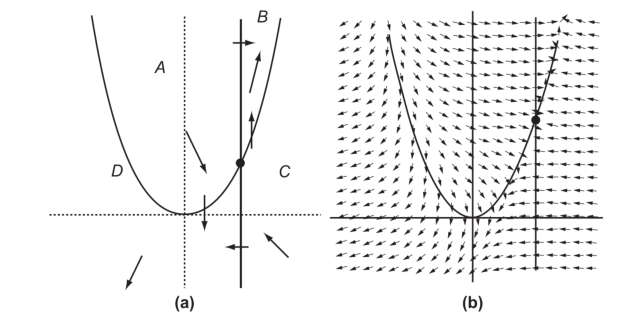
\includegraphics[width=0.7\textwidth]{../images/nullklinen.pdf}
        \end{center}
    \end{frame}
    \begin{frame}
    \frametitle{Kugeloberfläche}
        \begin{center}
            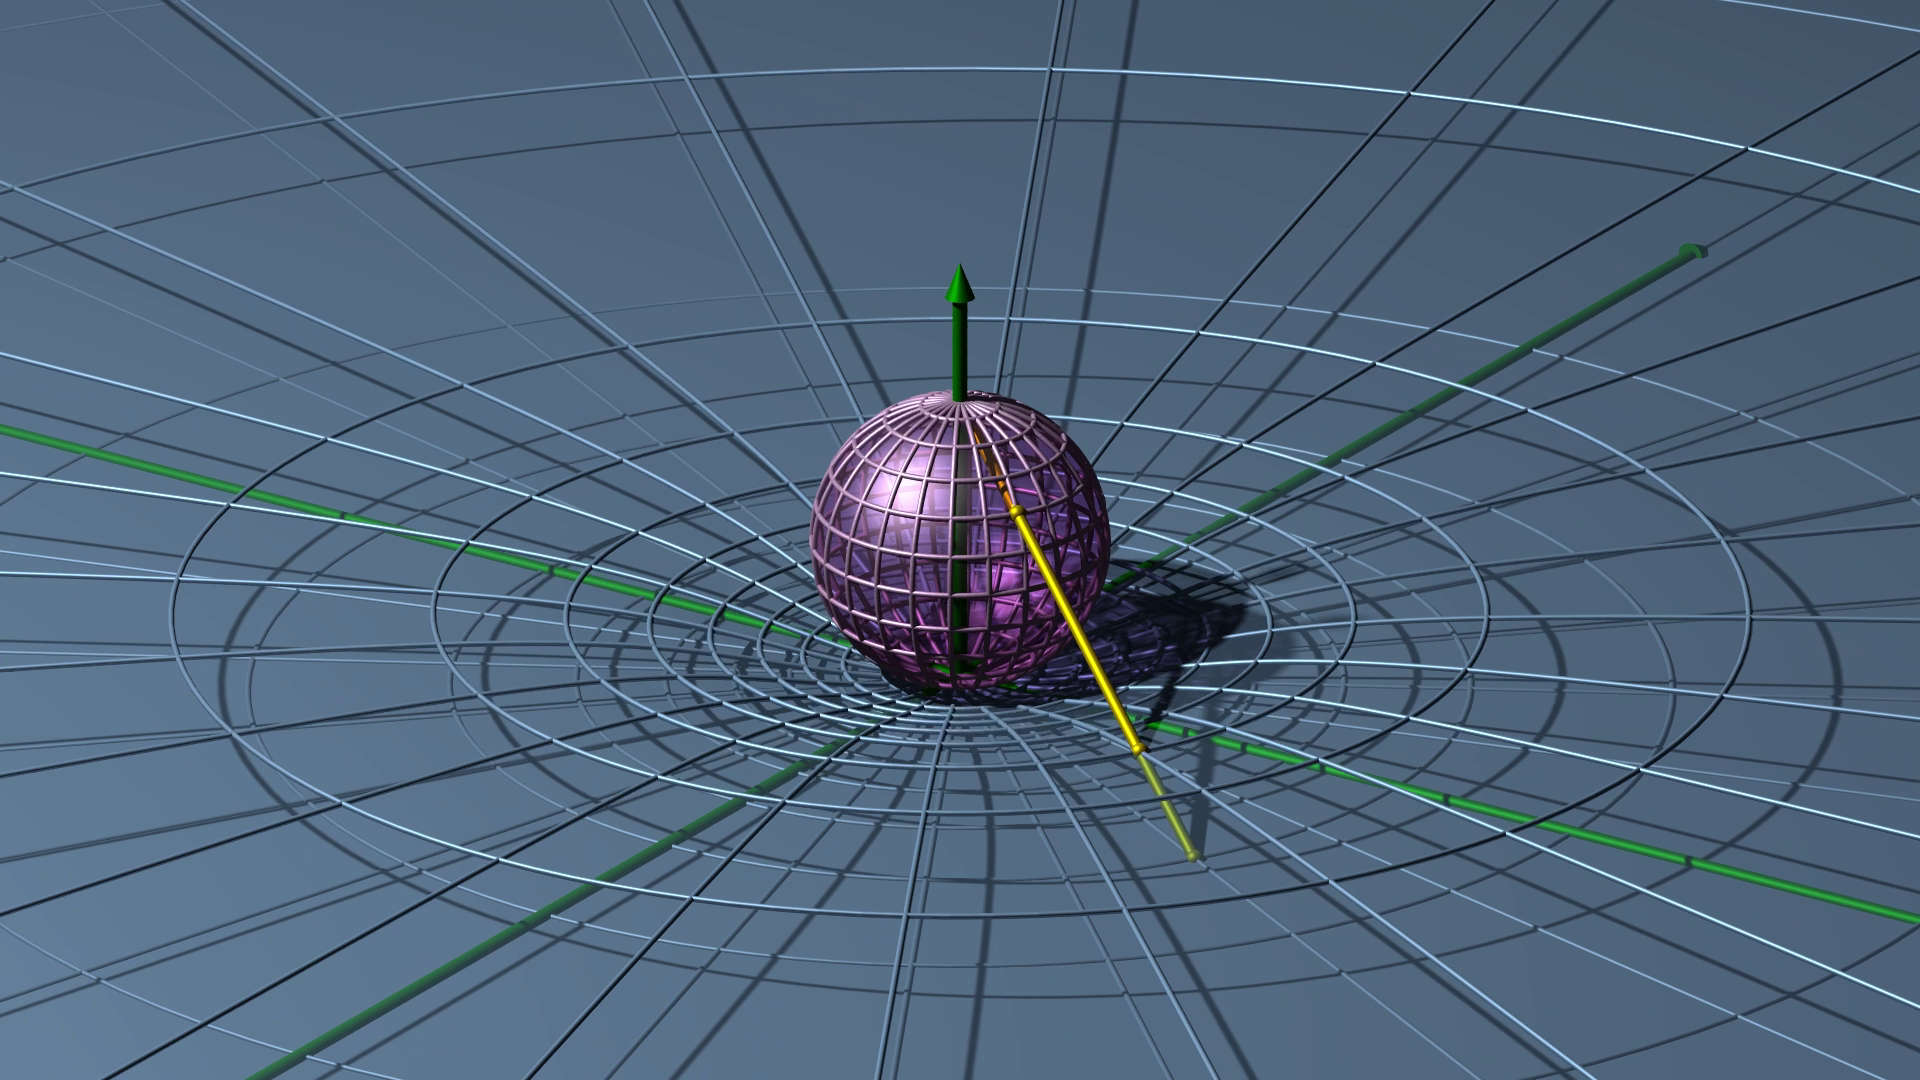
\includegraphics[width=0.7\textwidth]{../images/kugel_animation_thumbnail.jpg}
        \end{center}
    \end{frame}
    \begin{frame}
    \frametitle{Voraussetzungen für Poincaré-Bendixson}
        \begin{itemize}
            \item Dynamisches System $\Phi_t(p) \in \Xi^r(\mathbb{S}^2)$
            \item Finite Anzahl Singularitäten
            \item Anfangspunkt $p \in \mathbb{S}^2$
        \end{itemize}
    \end{frame}
    %Idee: 2D schränkt mögliche Lösungen stark ein. Das kann formuliert werden mit Poinbendix.
    % Wir brauchen dass, da unser ENSO model sehr stark vereinfacht ist.

    \section{Anwendung und Relevanz}

    \begin{frame}
    \frametitle{Lösungen Recharge Oszillator bei unterschiedlichen Anfangswerten}
        \begin{center}
            %% Creator: Matplotlib, PGF backend
%%
%% To include the figure in your LaTeX document, write
%%   \input{<filename>.pgf}
%%
%% Make sure the required packages are loaded in your preamble
%%   \usepackage{pgf}
%%
%% Also ensure that all the required font packages are loaded; for instance,
%% the lmodern package is sometimes necessary when using math font.
%%   \usepackage{lmodern}
%%
%% Figures using additional raster images can only be included by \input if
%% they are in the same directory as the main LaTeX file. For loading figures
%% from other directories you can use the `import` package
%%   \usepackage{import}
%%
%% and then include the figures with
%%   \import{<path to file>}{<filename>.pgf}
%%
%% Matplotlib used the following preamble
%%   \usepackage{bm}
%%   \usepackage{amsmath}
%%   \usepackage{xcolor}
%%   \usepackage{tgtermes}
%%   \makeatletter\@ifpackageloaded{underscore}{}{\usepackage[strings]{underscore}}\makeatother
%%
\begingroup%
\makeatletter%
\begin{pgfpicture}%
\pgfpathrectangle{\pgfpointorigin}{\pgfqpoint{4.500000in}{2.500000in}}%
\pgfusepath{use as bounding box, clip}%
\begin{pgfscope}%
\pgfsetbuttcap%
\pgfsetmiterjoin%
\definecolor{currentfill}{rgb}{1.000000,1.000000,1.000000}%
\pgfsetfillcolor{currentfill}%
\pgfsetlinewidth{0.000000pt}%
\definecolor{currentstroke}{rgb}{1.000000,1.000000,1.000000}%
\pgfsetstrokecolor{currentstroke}%
\pgfsetdash{}{0pt}%
\pgfpathmoveto{\pgfqpoint{0.000000in}{0.000000in}}%
\pgfpathlineto{\pgfqpoint{4.500000in}{0.000000in}}%
\pgfpathlineto{\pgfqpoint{4.500000in}{2.500000in}}%
\pgfpathlineto{\pgfqpoint{0.000000in}{2.500000in}}%
\pgfpathlineto{\pgfqpoint{0.000000in}{0.000000in}}%
\pgfpathclose%
\pgfusepath{fill}%
\end{pgfscope}%
\begin{pgfscope}%
\pgfsetbuttcap%
\pgfsetmiterjoin%
\definecolor{currentfill}{rgb}{1.000000,1.000000,1.000000}%
\pgfsetfillcolor{currentfill}%
\pgfsetlinewidth{0.000000pt}%
\definecolor{currentstroke}{rgb}{0.000000,0.000000,0.000000}%
\pgfsetstrokecolor{currentstroke}%
\pgfsetstrokeopacity{0.000000}%
\pgfsetdash{}{0pt}%
\pgfpathmoveto{\pgfqpoint{0.562500in}{0.275000in}}%
\pgfpathlineto{\pgfqpoint{4.050000in}{0.275000in}}%
\pgfpathlineto{\pgfqpoint{4.050000in}{2.200000in}}%
\pgfpathlineto{\pgfqpoint{0.562500in}{2.200000in}}%
\pgfpathlineto{\pgfqpoint{0.562500in}{0.275000in}}%
\pgfpathclose%
\pgfusepath{fill}%
\end{pgfscope}%
\begin{pgfscope}%
\pgfpathrectangle{\pgfqpoint{0.562500in}{0.275000in}}{\pgfqpoint{3.487500in}{1.925000in}}%
\pgfusepath{clip}%
\pgfsetbuttcap%
\pgfsetroundjoin%
\pgfsetlinewidth{0.250937pt}%
\definecolor{currentstroke}{rgb}{0.501961,0.501961,0.501961}%
\pgfsetstrokecolor{currentstroke}%
\pgfsetdash{{0.250000pt}{0.412500pt}}{0.000000pt}%
\pgfpathmoveto{\pgfqpoint{0.789946in}{0.275000in}}%
\pgfpathlineto{\pgfqpoint{0.789946in}{2.200000in}}%
\pgfusepath{stroke}%
\end{pgfscope}%
\begin{pgfscope}%
\pgfsetbuttcap%
\pgfsetroundjoin%
\definecolor{currentfill}{rgb}{0.000000,0.000000,0.000000}%
\pgfsetfillcolor{currentfill}%
\pgfsetlinewidth{0.501875pt}%
\definecolor{currentstroke}{rgb}{0.000000,0.000000,0.000000}%
\pgfsetstrokecolor{currentstroke}%
\pgfsetdash{}{0pt}%
\pgfsys@defobject{currentmarker}{\pgfqpoint{0.000000in}{-0.041667in}}{\pgfqpoint{0.000000in}{0.000000in}}{%
\pgfpathmoveto{\pgfqpoint{0.000000in}{0.000000in}}%
\pgfpathlineto{\pgfqpoint{0.000000in}{-0.041667in}}%
\pgfusepath{stroke,fill}%
}%
\begin{pgfscope}%
\pgfsys@transformshift{0.789946in}{0.275000in}%
\pgfsys@useobject{currentmarker}{}%
\end{pgfscope}%
\end{pgfscope}%
\begin{pgfscope}%
\definecolor{textcolor}{rgb}{0.000000,0.000000,0.000000}%
\pgfsetstrokecolor{textcolor}%
\pgfsetfillcolor{textcolor}%
\pgftext[x=0.789946in,y=0.184722in,,top]{\color{textcolor}\rmfamily\fontsize{10.000000}{12.000000}\selectfont \(\displaystyle {-1.0}\)}%
\end{pgfscope}%
\begin{pgfscope}%
\pgfpathrectangle{\pgfqpoint{0.562500in}{0.275000in}}{\pgfqpoint{3.487500in}{1.925000in}}%
\pgfusepath{clip}%
\pgfsetbuttcap%
\pgfsetroundjoin%
\pgfsetlinewidth{0.250937pt}%
\definecolor{currentstroke}{rgb}{0.501961,0.501961,0.501961}%
\pgfsetstrokecolor{currentstroke}%
\pgfsetdash{{0.250000pt}{0.412500pt}}{0.000000pt}%
\pgfpathmoveto{\pgfqpoint{1.548098in}{0.275000in}}%
\pgfpathlineto{\pgfqpoint{1.548098in}{2.200000in}}%
\pgfusepath{stroke}%
\end{pgfscope}%
\begin{pgfscope}%
\pgfsetbuttcap%
\pgfsetroundjoin%
\definecolor{currentfill}{rgb}{0.000000,0.000000,0.000000}%
\pgfsetfillcolor{currentfill}%
\pgfsetlinewidth{0.501875pt}%
\definecolor{currentstroke}{rgb}{0.000000,0.000000,0.000000}%
\pgfsetstrokecolor{currentstroke}%
\pgfsetdash{}{0pt}%
\pgfsys@defobject{currentmarker}{\pgfqpoint{0.000000in}{-0.041667in}}{\pgfqpoint{0.000000in}{0.000000in}}{%
\pgfpathmoveto{\pgfqpoint{0.000000in}{0.000000in}}%
\pgfpathlineto{\pgfqpoint{0.000000in}{-0.041667in}}%
\pgfusepath{stroke,fill}%
}%
\begin{pgfscope}%
\pgfsys@transformshift{1.548098in}{0.275000in}%
\pgfsys@useobject{currentmarker}{}%
\end{pgfscope}%
\end{pgfscope}%
\begin{pgfscope}%
\definecolor{textcolor}{rgb}{0.000000,0.000000,0.000000}%
\pgfsetstrokecolor{textcolor}%
\pgfsetfillcolor{textcolor}%
\pgftext[x=1.548098in,y=0.184722in,,top]{\color{textcolor}\rmfamily\fontsize{10.000000}{12.000000}\selectfont \(\displaystyle {-0.5}\)}%
\end{pgfscope}%
\begin{pgfscope}%
\pgfpathrectangle{\pgfqpoint{0.562500in}{0.275000in}}{\pgfqpoint{3.487500in}{1.925000in}}%
\pgfusepath{clip}%
\pgfsetbuttcap%
\pgfsetroundjoin%
\pgfsetlinewidth{0.250937pt}%
\definecolor{currentstroke}{rgb}{0.501961,0.501961,0.501961}%
\pgfsetstrokecolor{currentstroke}%
\pgfsetdash{{0.250000pt}{0.412500pt}}{0.000000pt}%
\pgfpathmoveto{\pgfqpoint{2.306250in}{0.275000in}}%
\pgfpathlineto{\pgfqpoint{2.306250in}{2.200000in}}%
\pgfusepath{stroke}%
\end{pgfscope}%
\begin{pgfscope}%
\pgfsetbuttcap%
\pgfsetroundjoin%
\definecolor{currentfill}{rgb}{0.000000,0.000000,0.000000}%
\pgfsetfillcolor{currentfill}%
\pgfsetlinewidth{0.501875pt}%
\definecolor{currentstroke}{rgb}{0.000000,0.000000,0.000000}%
\pgfsetstrokecolor{currentstroke}%
\pgfsetdash{}{0pt}%
\pgfsys@defobject{currentmarker}{\pgfqpoint{0.000000in}{-0.041667in}}{\pgfqpoint{0.000000in}{0.000000in}}{%
\pgfpathmoveto{\pgfqpoint{0.000000in}{0.000000in}}%
\pgfpathlineto{\pgfqpoint{0.000000in}{-0.041667in}}%
\pgfusepath{stroke,fill}%
}%
\begin{pgfscope}%
\pgfsys@transformshift{2.306250in}{0.275000in}%
\pgfsys@useobject{currentmarker}{}%
\end{pgfscope}%
\end{pgfscope}%
\begin{pgfscope}%
\definecolor{textcolor}{rgb}{0.000000,0.000000,0.000000}%
\pgfsetstrokecolor{textcolor}%
\pgfsetfillcolor{textcolor}%
\pgftext[x=2.306250in,y=0.184722in,,top]{\color{textcolor}\rmfamily\fontsize{10.000000}{12.000000}\selectfont \(\displaystyle {0.0}\)}%
\end{pgfscope}%
\begin{pgfscope}%
\pgfpathrectangle{\pgfqpoint{0.562500in}{0.275000in}}{\pgfqpoint{3.487500in}{1.925000in}}%
\pgfusepath{clip}%
\pgfsetbuttcap%
\pgfsetroundjoin%
\pgfsetlinewidth{0.250937pt}%
\definecolor{currentstroke}{rgb}{0.501961,0.501961,0.501961}%
\pgfsetstrokecolor{currentstroke}%
\pgfsetdash{{0.250000pt}{0.412500pt}}{0.000000pt}%
\pgfpathmoveto{\pgfqpoint{3.064402in}{0.275000in}}%
\pgfpathlineto{\pgfqpoint{3.064402in}{2.200000in}}%
\pgfusepath{stroke}%
\end{pgfscope}%
\begin{pgfscope}%
\pgfsetbuttcap%
\pgfsetroundjoin%
\definecolor{currentfill}{rgb}{0.000000,0.000000,0.000000}%
\pgfsetfillcolor{currentfill}%
\pgfsetlinewidth{0.501875pt}%
\definecolor{currentstroke}{rgb}{0.000000,0.000000,0.000000}%
\pgfsetstrokecolor{currentstroke}%
\pgfsetdash{}{0pt}%
\pgfsys@defobject{currentmarker}{\pgfqpoint{0.000000in}{-0.041667in}}{\pgfqpoint{0.000000in}{0.000000in}}{%
\pgfpathmoveto{\pgfqpoint{0.000000in}{0.000000in}}%
\pgfpathlineto{\pgfqpoint{0.000000in}{-0.041667in}}%
\pgfusepath{stroke,fill}%
}%
\begin{pgfscope}%
\pgfsys@transformshift{3.064402in}{0.275000in}%
\pgfsys@useobject{currentmarker}{}%
\end{pgfscope}%
\end{pgfscope}%
\begin{pgfscope}%
\definecolor{textcolor}{rgb}{0.000000,0.000000,0.000000}%
\pgfsetstrokecolor{textcolor}%
\pgfsetfillcolor{textcolor}%
\pgftext[x=3.064402in,y=0.184722in,,top]{\color{textcolor}\rmfamily\fontsize{10.000000}{12.000000}\selectfont \(\displaystyle {0.5}\)}%
\end{pgfscope}%
\begin{pgfscope}%
\pgfpathrectangle{\pgfqpoint{0.562500in}{0.275000in}}{\pgfqpoint{3.487500in}{1.925000in}}%
\pgfusepath{clip}%
\pgfsetbuttcap%
\pgfsetroundjoin%
\pgfsetlinewidth{0.250937pt}%
\definecolor{currentstroke}{rgb}{0.501961,0.501961,0.501961}%
\pgfsetstrokecolor{currentstroke}%
\pgfsetdash{{0.250000pt}{0.412500pt}}{0.000000pt}%
\pgfpathmoveto{\pgfqpoint{3.822554in}{0.275000in}}%
\pgfpathlineto{\pgfqpoint{3.822554in}{2.200000in}}%
\pgfusepath{stroke}%
\end{pgfscope}%
\begin{pgfscope}%
\pgfsetbuttcap%
\pgfsetroundjoin%
\definecolor{currentfill}{rgb}{0.000000,0.000000,0.000000}%
\pgfsetfillcolor{currentfill}%
\pgfsetlinewidth{0.501875pt}%
\definecolor{currentstroke}{rgb}{0.000000,0.000000,0.000000}%
\pgfsetstrokecolor{currentstroke}%
\pgfsetdash{}{0pt}%
\pgfsys@defobject{currentmarker}{\pgfqpoint{0.000000in}{-0.041667in}}{\pgfqpoint{0.000000in}{0.000000in}}{%
\pgfpathmoveto{\pgfqpoint{0.000000in}{0.000000in}}%
\pgfpathlineto{\pgfqpoint{0.000000in}{-0.041667in}}%
\pgfusepath{stroke,fill}%
}%
\begin{pgfscope}%
\pgfsys@transformshift{3.822554in}{0.275000in}%
\pgfsys@useobject{currentmarker}{}%
\end{pgfscope}%
\end{pgfscope}%
\begin{pgfscope}%
\definecolor{textcolor}{rgb}{0.000000,0.000000,0.000000}%
\pgfsetstrokecolor{textcolor}%
\pgfsetfillcolor{textcolor}%
\pgftext[x=3.822554in,y=0.184722in,,top]{\color{textcolor}\rmfamily\fontsize{10.000000}{12.000000}\selectfont \(\displaystyle {1.0}\)}%
\end{pgfscope}%
\begin{pgfscope}%
\pgfpathrectangle{\pgfqpoint{0.562500in}{0.275000in}}{\pgfqpoint{3.487500in}{1.925000in}}%
\pgfusepath{clip}%
\pgfsetbuttcap%
\pgfsetroundjoin%
\pgfsetlinewidth{0.250937pt}%
\definecolor{currentstroke}{rgb}{0.501961,0.501961,0.501961}%
\pgfsetstrokecolor{currentstroke}%
\pgfsetdash{{0.250000pt}{0.412500pt}}{0.000000pt}%
\pgfpathmoveto{\pgfqpoint{0.562500in}{0.388235in}}%
\pgfpathlineto{\pgfqpoint{4.050000in}{0.388235in}}%
\pgfusepath{stroke}%
\end{pgfscope}%
\begin{pgfscope}%
\pgfsetbuttcap%
\pgfsetroundjoin%
\definecolor{currentfill}{rgb}{0.000000,0.000000,0.000000}%
\pgfsetfillcolor{currentfill}%
\pgfsetlinewidth{0.501875pt}%
\definecolor{currentstroke}{rgb}{0.000000,0.000000,0.000000}%
\pgfsetstrokecolor{currentstroke}%
\pgfsetdash{}{0pt}%
\pgfsys@defobject{currentmarker}{\pgfqpoint{-0.041667in}{0.000000in}}{\pgfqpoint{-0.000000in}{0.000000in}}{%
\pgfpathmoveto{\pgfqpoint{-0.000000in}{0.000000in}}%
\pgfpathlineto{\pgfqpoint{-0.041667in}{0.000000in}}%
\pgfusepath{stroke,fill}%
}%
\begin{pgfscope}%
\pgfsys@transformshift{0.562500in}{0.388235in}%
\pgfsys@useobject{currentmarker}{}%
\end{pgfscope}%
\end{pgfscope}%
\begin{pgfscope}%
\definecolor{textcolor}{rgb}{0.000000,0.000000,0.000000}%
\pgfsetstrokecolor{textcolor}%
\pgfsetfillcolor{textcolor}%
\pgftext[x=0.294752in, y=0.341534in, left, base]{\color{textcolor}\rmfamily\fontsize{10.000000}{12.000000}\selectfont \(\displaystyle {-1}\)}%
\end{pgfscope}%
\begin{pgfscope}%
\pgfpathrectangle{\pgfqpoint{0.562500in}{0.275000in}}{\pgfqpoint{3.487500in}{1.925000in}}%
\pgfusepath{clip}%
\pgfsetbuttcap%
\pgfsetroundjoin%
\pgfsetlinewidth{0.250937pt}%
\definecolor{currentstroke}{rgb}{0.501961,0.501961,0.501961}%
\pgfsetstrokecolor{currentstroke}%
\pgfsetdash{{0.250000pt}{0.412500pt}}{0.000000pt}%
\pgfpathmoveto{\pgfqpoint{0.562500in}{0.954412in}}%
\pgfpathlineto{\pgfqpoint{4.050000in}{0.954412in}}%
\pgfusepath{stroke}%
\end{pgfscope}%
\begin{pgfscope}%
\pgfsetbuttcap%
\pgfsetroundjoin%
\definecolor{currentfill}{rgb}{0.000000,0.000000,0.000000}%
\pgfsetfillcolor{currentfill}%
\pgfsetlinewidth{0.501875pt}%
\definecolor{currentstroke}{rgb}{0.000000,0.000000,0.000000}%
\pgfsetstrokecolor{currentstroke}%
\pgfsetdash{}{0pt}%
\pgfsys@defobject{currentmarker}{\pgfqpoint{-0.041667in}{0.000000in}}{\pgfqpoint{-0.000000in}{0.000000in}}{%
\pgfpathmoveto{\pgfqpoint{-0.000000in}{0.000000in}}%
\pgfpathlineto{\pgfqpoint{-0.041667in}{0.000000in}}%
\pgfusepath{stroke,fill}%
}%
\begin{pgfscope}%
\pgfsys@transformshift{0.562500in}{0.954412in}%
\pgfsys@useobject{currentmarker}{}%
\end{pgfscope}%
\end{pgfscope}%
\begin{pgfscope}%
\definecolor{textcolor}{rgb}{0.000000,0.000000,0.000000}%
\pgfsetstrokecolor{textcolor}%
\pgfsetfillcolor{textcolor}%
\pgftext[x=0.402777in, y=0.907711in, left, base]{\color{textcolor}\rmfamily\fontsize{10.000000}{12.000000}\selectfont \(\displaystyle {0}\)}%
\end{pgfscope}%
\begin{pgfscope}%
\pgfpathrectangle{\pgfqpoint{0.562500in}{0.275000in}}{\pgfqpoint{3.487500in}{1.925000in}}%
\pgfusepath{clip}%
\pgfsetbuttcap%
\pgfsetroundjoin%
\pgfsetlinewidth{0.250937pt}%
\definecolor{currentstroke}{rgb}{0.501961,0.501961,0.501961}%
\pgfsetstrokecolor{currentstroke}%
\pgfsetdash{{0.250000pt}{0.412500pt}}{0.000000pt}%
\pgfpathmoveto{\pgfqpoint{0.562500in}{1.520588in}}%
\pgfpathlineto{\pgfqpoint{4.050000in}{1.520588in}}%
\pgfusepath{stroke}%
\end{pgfscope}%
\begin{pgfscope}%
\pgfsetbuttcap%
\pgfsetroundjoin%
\definecolor{currentfill}{rgb}{0.000000,0.000000,0.000000}%
\pgfsetfillcolor{currentfill}%
\pgfsetlinewidth{0.501875pt}%
\definecolor{currentstroke}{rgb}{0.000000,0.000000,0.000000}%
\pgfsetstrokecolor{currentstroke}%
\pgfsetdash{}{0pt}%
\pgfsys@defobject{currentmarker}{\pgfqpoint{-0.041667in}{0.000000in}}{\pgfqpoint{-0.000000in}{0.000000in}}{%
\pgfpathmoveto{\pgfqpoint{-0.000000in}{0.000000in}}%
\pgfpathlineto{\pgfqpoint{-0.041667in}{0.000000in}}%
\pgfusepath{stroke,fill}%
}%
\begin{pgfscope}%
\pgfsys@transformshift{0.562500in}{1.520588in}%
\pgfsys@useobject{currentmarker}{}%
\end{pgfscope}%
\end{pgfscope}%
\begin{pgfscope}%
\definecolor{textcolor}{rgb}{0.000000,0.000000,0.000000}%
\pgfsetstrokecolor{textcolor}%
\pgfsetfillcolor{textcolor}%
\pgftext[x=0.402777in, y=1.473887in, left, base]{\color{textcolor}\rmfamily\fontsize{10.000000}{12.000000}\selectfont \(\displaystyle {1}\)}%
\end{pgfscope}%
\begin{pgfscope}%
\pgfpathrectangle{\pgfqpoint{0.562500in}{0.275000in}}{\pgfqpoint{3.487500in}{1.925000in}}%
\pgfusepath{clip}%
\pgfsetbuttcap%
\pgfsetroundjoin%
\pgfsetlinewidth{0.250937pt}%
\definecolor{currentstroke}{rgb}{0.501961,0.501961,0.501961}%
\pgfsetstrokecolor{currentstroke}%
\pgfsetdash{{0.250000pt}{0.412500pt}}{0.000000pt}%
\pgfpathmoveto{\pgfqpoint{0.562500in}{2.086765in}}%
\pgfpathlineto{\pgfqpoint{4.050000in}{2.086765in}}%
\pgfusepath{stroke}%
\end{pgfscope}%
\begin{pgfscope}%
\pgfsetbuttcap%
\pgfsetroundjoin%
\definecolor{currentfill}{rgb}{0.000000,0.000000,0.000000}%
\pgfsetfillcolor{currentfill}%
\pgfsetlinewidth{0.501875pt}%
\definecolor{currentstroke}{rgb}{0.000000,0.000000,0.000000}%
\pgfsetstrokecolor{currentstroke}%
\pgfsetdash{}{0pt}%
\pgfsys@defobject{currentmarker}{\pgfqpoint{-0.041667in}{0.000000in}}{\pgfqpoint{-0.000000in}{0.000000in}}{%
\pgfpathmoveto{\pgfqpoint{-0.000000in}{0.000000in}}%
\pgfpathlineto{\pgfqpoint{-0.041667in}{0.000000in}}%
\pgfusepath{stroke,fill}%
}%
\begin{pgfscope}%
\pgfsys@transformshift{0.562500in}{2.086765in}%
\pgfsys@useobject{currentmarker}{}%
\end{pgfscope}%
\end{pgfscope}%
\begin{pgfscope}%
\definecolor{textcolor}{rgb}{0.000000,0.000000,0.000000}%
\pgfsetstrokecolor{textcolor}%
\pgfsetfillcolor{textcolor}%
\pgftext[x=0.402777in, y=2.040063in, left, base]{\color{textcolor}\rmfamily\fontsize{10.000000}{12.000000}\selectfont \(\displaystyle {2}\)}%
\end{pgfscope}%
\begin{pgfscope}%
\pgfpathrectangle{\pgfqpoint{0.562500in}{0.275000in}}{\pgfqpoint{3.487500in}{1.925000in}}%
\pgfusepath{clip}%
\pgfsetbuttcap%
\pgfsetroundjoin%
\definecolor{currentfill}{rgb}{0.121569,0.466667,0.705882}%
\pgfsetfillcolor{currentfill}%
\pgfsetlinewidth{1.003750pt}%
\definecolor{currentstroke}{rgb}{0.121569,0.466667,0.705882}%
\pgfsetstrokecolor{currentstroke}%
\pgfsetdash{}{0pt}%
\pgfsys@defobject{currentmarker}{\pgfqpoint{-0.020833in}{-0.020833in}}{\pgfqpoint{0.020833in}{0.020833in}}{%
\pgfpathmoveto{\pgfqpoint{0.000000in}{-0.020833in}}%
\pgfpathcurveto{\pgfqpoint{0.005525in}{-0.020833in}}{\pgfqpoint{0.010825in}{-0.018638in}}{\pgfqpoint{0.014731in}{-0.014731in}}%
\pgfpathcurveto{\pgfqpoint{0.018638in}{-0.010825in}}{\pgfqpoint{0.020833in}{-0.005525in}}{\pgfqpoint{0.020833in}{0.000000in}}%
\pgfpathcurveto{\pgfqpoint{0.020833in}{0.005525in}}{\pgfqpoint{0.018638in}{0.010825in}}{\pgfqpoint{0.014731in}{0.014731in}}%
\pgfpathcurveto{\pgfqpoint{0.010825in}{0.018638in}}{\pgfqpoint{0.005525in}{0.020833in}}{\pgfqpoint{0.000000in}{0.020833in}}%
\pgfpathcurveto{\pgfqpoint{-0.005525in}{0.020833in}}{\pgfqpoint{-0.010825in}{0.018638in}}{\pgfqpoint{-0.014731in}{0.014731in}}%
\pgfpathcurveto{\pgfqpoint{-0.018638in}{0.010825in}}{\pgfqpoint{-0.020833in}{0.005525in}}{\pgfqpoint{-0.020833in}{0.000000in}}%
\pgfpathcurveto{\pgfqpoint{-0.020833in}{-0.005525in}}{\pgfqpoint{-0.018638in}{-0.010825in}}{\pgfqpoint{-0.014731in}{-0.014731in}}%
\pgfpathcurveto{\pgfqpoint{-0.010825in}{-0.018638in}}{\pgfqpoint{-0.005525in}{-0.020833in}}{\pgfqpoint{0.000000in}{-0.020833in}}%
\pgfpathlineto{\pgfqpoint{0.000000in}{-0.020833in}}%
\pgfpathclose%
\pgfusepath{stroke,fill}%
}%
\begin{pgfscope}%
\pgfsys@transformshift{2.306250in}{0.954412in}%
\pgfsys@useobject{currentmarker}{}%
\end{pgfscope}%
\begin{pgfscope}%
\pgfsys@transformshift{2.306250in}{0.954412in}%
\pgfsys@useobject{currentmarker}{}%
\end{pgfscope}%
\begin{pgfscope}%
\pgfsys@transformshift{2.306250in}{0.954412in}%
\pgfsys@useobject{currentmarker}{}%
\end{pgfscope}%
\begin{pgfscope}%
\pgfsys@transformshift{2.306250in}{0.954412in}%
\pgfsys@useobject{currentmarker}{}%
\end{pgfscope}%
\begin{pgfscope}%
\pgfsys@transformshift{2.306250in}{0.954412in}%
\pgfsys@useobject{currentmarker}{}%
\end{pgfscope}%
\begin{pgfscope}%
\pgfsys@transformshift{2.306250in}{0.954412in}%
\pgfsys@useobject{currentmarker}{}%
\end{pgfscope}%
\begin{pgfscope}%
\pgfsys@transformshift{2.306250in}{0.954412in}%
\pgfsys@useobject{currentmarker}{}%
\end{pgfscope}%
\begin{pgfscope}%
\pgfsys@transformshift{2.306250in}{0.954412in}%
\pgfsys@useobject{currentmarker}{}%
\end{pgfscope}%
\begin{pgfscope}%
\pgfsys@transformshift{2.306250in}{0.954412in}%
\pgfsys@useobject{currentmarker}{}%
\end{pgfscope}%
\begin{pgfscope}%
\pgfsys@transformshift{2.306250in}{0.954412in}%
\pgfsys@useobject{currentmarker}{}%
\end{pgfscope}%
\begin{pgfscope}%
\pgfsys@transformshift{2.306250in}{0.954412in}%
\pgfsys@useobject{currentmarker}{}%
\end{pgfscope}%
\begin{pgfscope}%
\pgfsys@transformshift{2.306250in}{0.954412in}%
\pgfsys@useobject{currentmarker}{}%
\end{pgfscope}%
\begin{pgfscope}%
\pgfsys@transformshift{2.306250in}{0.954412in}%
\pgfsys@useobject{currentmarker}{}%
\end{pgfscope}%
\begin{pgfscope}%
\pgfsys@transformshift{2.306250in}{0.954412in}%
\pgfsys@useobject{currentmarker}{}%
\end{pgfscope}%
\begin{pgfscope}%
\pgfsys@transformshift{2.306250in}{0.954412in}%
\pgfsys@useobject{currentmarker}{}%
\end{pgfscope}%
\begin{pgfscope}%
\pgfsys@transformshift{2.306250in}{0.954412in}%
\pgfsys@useobject{currentmarker}{}%
\end{pgfscope}%
\begin{pgfscope}%
\pgfsys@transformshift{2.306250in}{0.954412in}%
\pgfsys@useobject{currentmarker}{}%
\end{pgfscope}%
\begin{pgfscope}%
\pgfsys@transformshift{2.306250in}{0.954412in}%
\pgfsys@useobject{currentmarker}{}%
\end{pgfscope}%
\begin{pgfscope}%
\pgfsys@transformshift{2.306250in}{0.954412in}%
\pgfsys@useobject{currentmarker}{}%
\end{pgfscope}%
\begin{pgfscope}%
\pgfsys@transformshift{2.306250in}{0.954412in}%
\pgfsys@useobject{currentmarker}{}%
\end{pgfscope}%
\begin{pgfscope}%
\pgfsys@transformshift{2.306250in}{0.954412in}%
\pgfsys@useobject{currentmarker}{}%
\end{pgfscope}%
\begin{pgfscope}%
\pgfsys@transformshift{2.306250in}{0.954412in}%
\pgfsys@useobject{currentmarker}{}%
\end{pgfscope}%
\begin{pgfscope}%
\pgfsys@transformshift{2.306250in}{0.954412in}%
\pgfsys@useobject{currentmarker}{}%
\end{pgfscope}%
\begin{pgfscope}%
\pgfsys@transformshift{2.306250in}{0.954412in}%
\pgfsys@useobject{currentmarker}{}%
\end{pgfscope}%
\begin{pgfscope}%
\pgfsys@transformshift{2.306250in}{0.954412in}%
\pgfsys@useobject{currentmarker}{}%
\end{pgfscope}%
\begin{pgfscope}%
\pgfsys@transformshift{2.306250in}{0.954412in}%
\pgfsys@useobject{currentmarker}{}%
\end{pgfscope}%
\begin{pgfscope}%
\pgfsys@transformshift{2.306250in}{0.954412in}%
\pgfsys@useobject{currentmarker}{}%
\end{pgfscope}%
\begin{pgfscope}%
\pgfsys@transformshift{2.306250in}{0.954412in}%
\pgfsys@useobject{currentmarker}{}%
\end{pgfscope}%
\begin{pgfscope}%
\pgfsys@transformshift{2.306250in}{0.954412in}%
\pgfsys@useobject{currentmarker}{}%
\end{pgfscope}%
\begin{pgfscope}%
\pgfsys@transformshift{2.306250in}{0.954412in}%
\pgfsys@useobject{currentmarker}{}%
\end{pgfscope}%
\begin{pgfscope}%
\pgfsys@transformshift{2.306250in}{0.954412in}%
\pgfsys@useobject{currentmarker}{}%
\end{pgfscope}%
\begin{pgfscope}%
\pgfsys@transformshift{2.306250in}{0.954412in}%
\pgfsys@useobject{currentmarker}{}%
\end{pgfscope}%
\begin{pgfscope}%
\pgfsys@transformshift{2.306250in}{0.954412in}%
\pgfsys@useobject{currentmarker}{}%
\end{pgfscope}%
\begin{pgfscope}%
\pgfsys@transformshift{2.306250in}{0.954412in}%
\pgfsys@useobject{currentmarker}{}%
\end{pgfscope}%
\begin{pgfscope}%
\pgfsys@transformshift{2.306250in}{0.954412in}%
\pgfsys@useobject{currentmarker}{}%
\end{pgfscope}%
\begin{pgfscope}%
\pgfsys@transformshift{2.306250in}{0.954412in}%
\pgfsys@useobject{currentmarker}{}%
\end{pgfscope}%
\begin{pgfscope}%
\pgfsys@transformshift{2.306250in}{0.954412in}%
\pgfsys@useobject{currentmarker}{}%
\end{pgfscope}%
\begin{pgfscope}%
\pgfsys@transformshift{2.306250in}{0.954412in}%
\pgfsys@useobject{currentmarker}{}%
\end{pgfscope}%
\begin{pgfscope}%
\pgfsys@transformshift{2.306250in}{0.954412in}%
\pgfsys@useobject{currentmarker}{}%
\end{pgfscope}%
\begin{pgfscope}%
\pgfsys@transformshift{2.306250in}{0.954412in}%
\pgfsys@useobject{currentmarker}{}%
\end{pgfscope}%
\begin{pgfscope}%
\pgfsys@transformshift{2.306250in}{0.954412in}%
\pgfsys@useobject{currentmarker}{}%
\end{pgfscope}%
\begin{pgfscope}%
\pgfsys@transformshift{2.306250in}{0.954412in}%
\pgfsys@useobject{currentmarker}{}%
\end{pgfscope}%
\begin{pgfscope}%
\pgfsys@transformshift{2.306250in}{0.954412in}%
\pgfsys@useobject{currentmarker}{}%
\end{pgfscope}%
\begin{pgfscope}%
\pgfsys@transformshift{2.306250in}{0.954412in}%
\pgfsys@useobject{currentmarker}{}%
\end{pgfscope}%
\begin{pgfscope}%
\pgfsys@transformshift{2.306250in}{0.954412in}%
\pgfsys@useobject{currentmarker}{}%
\end{pgfscope}%
\begin{pgfscope}%
\pgfsys@transformshift{2.306250in}{0.954412in}%
\pgfsys@useobject{currentmarker}{}%
\end{pgfscope}%
\begin{pgfscope}%
\pgfsys@transformshift{2.306250in}{0.954412in}%
\pgfsys@useobject{currentmarker}{}%
\end{pgfscope}%
\begin{pgfscope}%
\pgfsys@transformshift{2.306250in}{0.954412in}%
\pgfsys@useobject{currentmarker}{}%
\end{pgfscope}%
\begin{pgfscope}%
\pgfsys@transformshift{2.306250in}{0.954412in}%
\pgfsys@useobject{currentmarker}{}%
\end{pgfscope}%
\begin{pgfscope}%
\pgfsys@transformshift{2.306250in}{0.954412in}%
\pgfsys@useobject{currentmarker}{}%
\end{pgfscope}%
\begin{pgfscope}%
\pgfsys@transformshift{2.306250in}{0.954412in}%
\pgfsys@useobject{currentmarker}{}%
\end{pgfscope}%
\begin{pgfscope}%
\pgfsys@transformshift{2.306250in}{0.954412in}%
\pgfsys@useobject{currentmarker}{}%
\end{pgfscope}%
\begin{pgfscope}%
\pgfsys@transformshift{2.306250in}{0.954412in}%
\pgfsys@useobject{currentmarker}{}%
\end{pgfscope}%
\begin{pgfscope}%
\pgfsys@transformshift{2.306250in}{0.954412in}%
\pgfsys@useobject{currentmarker}{}%
\end{pgfscope}%
\begin{pgfscope}%
\pgfsys@transformshift{2.306250in}{0.954412in}%
\pgfsys@useobject{currentmarker}{}%
\end{pgfscope}%
\begin{pgfscope}%
\pgfsys@transformshift{2.306250in}{0.954412in}%
\pgfsys@useobject{currentmarker}{}%
\end{pgfscope}%
\begin{pgfscope}%
\pgfsys@transformshift{2.306250in}{0.954412in}%
\pgfsys@useobject{currentmarker}{}%
\end{pgfscope}%
\begin{pgfscope}%
\pgfsys@transformshift{2.306250in}{0.954412in}%
\pgfsys@useobject{currentmarker}{}%
\end{pgfscope}%
\begin{pgfscope}%
\pgfsys@transformshift{2.306250in}{0.954412in}%
\pgfsys@useobject{currentmarker}{}%
\end{pgfscope}%
\begin{pgfscope}%
\pgfsys@transformshift{2.306250in}{0.954412in}%
\pgfsys@useobject{currentmarker}{}%
\end{pgfscope}%
\begin{pgfscope}%
\pgfsys@transformshift{2.306250in}{0.954412in}%
\pgfsys@useobject{currentmarker}{}%
\end{pgfscope}%
\begin{pgfscope}%
\pgfsys@transformshift{2.306250in}{0.954412in}%
\pgfsys@useobject{currentmarker}{}%
\end{pgfscope}%
\begin{pgfscope}%
\pgfsys@transformshift{2.306250in}{0.954412in}%
\pgfsys@useobject{currentmarker}{}%
\end{pgfscope}%
\begin{pgfscope}%
\pgfsys@transformshift{2.306250in}{0.954412in}%
\pgfsys@useobject{currentmarker}{}%
\end{pgfscope}%
\begin{pgfscope}%
\pgfsys@transformshift{2.306250in}{0.954412in}%
\pgfsys@useobject{currentmarker}{}%
\end{pgfscope}%
\begin{pgfscope}%
\pgfsys@transformshift{2.306250in}{0.954412in}%
\pgfsys@useobject{currentmarker}{}%
\end{pgfscope}%
\begin{pgfscope}%
\pgfsys@transformshift{2.306250in}{0.954412in}%
\pgfsys@useobject{currentmarker}{}%
\end{pgfscope}%
\begin{pgfscope}%
\pgfsys@transformshift{2.306250in}{0.954412in}%
\pgfsys@useobject{currentmarker}{}%
\end{pgfscope}%
\begin{pgfscope}%
\pgfsys@transformshift{2.306250in}{0.954412in}%
\pgfsys@useobject{currentmarker}{}%
\end{pgfscope}%
\begin{pgfscope}%
\pgfsys@transformshift{2.306250in}{0.954412in}%
\pgfsys@useobject{currentmarker}{}%
\end{pgfscope}%
\begin{pgfscope}%
\pgfsys@transformshift{2.306250in}{0.954412in}%
\pgfsys@useobject{currentmarker}{}%
\end{pgfscope}%
\begin{pgfscope}%
\pgfsys@transformshift{2.306250in}{0.954412in}%
\pgfsys@useobject{currentmarker}{}%
\end{pgfscope}%
\begin{pgfscope}%
\pgfsys@transformshift{2.306250in}{0.954412in}%
\pgfsys@useobject{currentmarker}{}%
\end{pgfscope}%
\begin{pgfscope}%
\pgfsys@transformshift{2.306250in}{0.954412in}%
\pgfsys@useobject{currentmarker}{}%
\end{pgfscope}%
\begin{pgfscope}%
\pgfsys@transformshift{2.306250in}{0.954412in}%
\pgfsys@useobject{currentmarker}{}%
\end{pgfscope}%
\begin{pgfscope}%
\pgfsys@transformshift{2.306250in}{0.954412in}%
\pgfsys@useobject{currentmarker}{}%
\end{pgfscope}%
\begin{pgfscope}%
\pgfsys@transformshift{2.306250in}{0.954412in}%
\pgfsys@useobject{currentmarker}{}%
\end{pgfscope}%
\begin{pgfscope}%
\pgfsys@transformshift{2.306250in}{0.954412in}%
\pgfsys@useobject{currentmarker}{}%
\end{pgfscope}%
\begin{pgfscope}%
\pgfsys@transformshift{2.306250in}{0.954412in}%
\pgfsys@useobject{currentmarker}{}%
\end{pgfscope}%
\begin{pgfscope}%
\pgfsys@transformshift{2.306250in}{0.954412in}%
\pgfsys@useobject{currentmarker}{}%
\end{pgfscope}%
\begin{pgfscope}%
\pgfsys@transformshift{2.306250in}{0.954412in}%
\pgfsys@useobject{currentmarker}{}%
\end{pgfscope}%
\begin{pgfscope}%
\pgfsys@transformshift{2.306250in}{0.954412in}%
\pgfsys@useobject{currentmarker}{}%
\end{pgfscope}%
\begin{pgfscope}%
\pgfsys@transformshift{2.306250in}{0.954412in}%
\pgfsys@useobject{currentmarker}{}%
\end{pgfscope}%
\begin{pgfscope}%
\pgfsys@transformshift{2.306250in}{0.954412in}%
\pgfsys@useobject{currentmarker}{}%
\end{pgfscope}%
\begin{pgfscope}%
\pgfsys@transformshift{2.306250in}{0.954412in}%
\pgfsys@useobject{currentmarker}{}%
\end{pgfscope}%
\begin{pgfscope}%
\pgfsys@transformshift{2.306250in}{0.954412in}%
\pgfsys@useobject{currentmarker}{}%
\end{pgfscope}%
\begin{pgfscope}%
\pgfsys@transformshift{2.306250in}{0.954412in}%
\pgfsys@useobject{currentmarker}{}%
\end{pgfscope}%
\begin{pgfscope}%
\pgfsys@transformshift{2.306250in}{0.954412in}%
\pgfsys@useobject{currentmarker}{}%
\end{pgfscope}%
\begin{pgfscope}%
\pgfsys@transformshift{2.306250in}{0.954412in}%
\pgfsys@useobject{currentmarker}{}%
\end{pgfscope}%
\begin{pgfscope}%
\pgfsys@transformshift{2.306250in}{0.954412in}%
\pgfsys@useobject{currentmarker}{}%
\end{pgfscope}%
\begin{pgfscope}%
\pgfsys@transformshift{2.306250in}{0.954412in}%
\pgfsys@useobject{currentmarker}{}%
\end{pgfscope}%
\begin{pgfscope}%
\pgfsys@transformshift{2.306250in}{0.954412in}%
\pgfsys@useobject{currentmarker}{}%
\end{pgfscope}%
\begin{pgfscope}%
\pgfsys@transformshift{2.306250in}{0.954412in}%
\pgfsys@useobject{currentmarker}{}%
\end{pgfscope}%
\begin{pgfscope}%
\pgfsys@transformshift{2.306250in}{0.954412in}%
\pgfsys@useobject{currentmarker}{}%
\end{pgfscope}%
\begin{pgfscope}%
\pgfsys@transformshift{2.306250in}{0.954412in}%
\pgfsys@useobject{currentmarker}{}%
\end{pgfscope}%
\begin{pgfscope}%
\pgfsys@transformshift{2.306250in}{0.954412in}%
\pgfsys@useobject{currentmarker}{}%
\end{pgfscope}%
\begin{pgfscope}%
\pgfsys@transformshift{2.306250in}{0.954412in}%
\pgfsys@useobject{currentmarker}{}%
\end{pgfscope}%
\begin{pgfscope}%
\pgfsys@transformshift{2.306250in}{0.954412in}%
\pgfsys@useobject{currentmarker}{}%
\end{pgfscope}%
\begin{pgfscope}%
\pgfsys@transformshift{2.306250in}{0.954412in}%
\pgfsys@useobject{currentmarker}{}%
\end{pgfscope}%
\begin{pgfscope}%
\pgfsys@transformshift{2.306250in}{0.954412in}%
\pgfsys@useobject{currentmarker}{}%
\end{pgfscope}%
\begin{pgfscope}%
\pgfsys@transformshift{2.306250in}{0.954412in}%
\pgfsys@useobject{currentmarker}{}%
\end{pgfscope}%
\begin{pgfscope}%
\pgfsys@transformshift{2.306250in}{0.954412in}%
\pgfsys@useobject{currentmarker}{}%
\end{pgfscope}%
\begin{pgfscope}%
\pgfsys@transformshift{2.306250in}{0.954412in}%
\pgfsys@useobject{currentmarker}{}%
\end{pgfscope}%
\begin{pgfscope}%
\pgfsys@transformshift{2.306250in}{0.954412in}%
\pgfsys@useobject{currentmarker}{}%
\end{pgfscope}%
\begin{pgfscope}%
\pgfsys@transformshift{2.306250in}{0.954412in}%
\pgfsys@useobject{currentmarker}{}%
\end{pgfscope}%
\begin{pgfscope}%
\pgfsys@transformshift{2.306250in}{0.954412in}%
\pgfsys@useobject{currentmarker}{}%
\end{pgfscope}%
\begin{pgfscope}%
\pgfsys@transformshift{2.306250in}{0.954412in}%
\pgfsys@useobject{currentmarker}{}%
\end{pgfscope}%
\begin{pgfscope}%
\pgfsys@transformshift{2.306250in}{0.954412in}%
\pgfsys@useobject{currentmarker}{}%
\end{pgfscope}%
\begin{pgfscope}%
\pgfsys@transformshift{2.306250in}{0.954412in}%
\pgfsys@useobject{currentmarker}{}%
\end{pgfscope}%
\begin{pgfscope}%
\pgfsys@transformshift{2.306250in}{0.954412in}%
\pgfsys@useobject{currentmarker}{}%
\end{pgfscope}%
\begin{pgfscope}%
\pgfsys@transformshift{2.306250in}{0.954412in}%
\pgfsys@useobject{currentmarker}{}%
\end{pgfscope}%
\begin{pgfscope}%
\pgfsys@transformshift{2.306250in}{0.954412in}%
\pgfsys@useobject{currentmarker}{}%
\end{pgfscope}%
\begin{pgfscope}%
\pgfsys@transformshift{2.306250in}{0.954412in}%
\pgfsys@useobject{currentmarker}{}%
\end{pgfscope}%
\begin{pgfscope}%
\pgfsys@transformshift{2.306250in}{0.954412in}%
\pgfsys@useobject{currentmarker}{}%
\end{pgfscope}%
\begin{pgfscope}%
\pgfsys@transformshift{2.306250in}{0.954412in}%
\pgfsys@useobject{currentmarker}{}%
\end{pgfscope}%
\begin{pgfscope}%
\pgfsys@transformshift{2.306250in}{0.954412in}%
\pgfsys@useobject{currentmarker}{}%
\end{pgfscope}%
\begin{pgfscope}%
\pgfsys@transformshift{2.306250in}{0.954412in}%
\pgfsys@useobject{currentmarker}{}%
\end{pgfscope}%
\begin{pgfscope}%
\pgfsys@transformshift{2.306250in}{0.954412in}%
\pgfsys@useobject{currentmarker}{}%
\end{pgfscope}%
\begin{pgfscope}%
\pgfsys@transformshift{2.306250in}{0.954412in}%
\pgfsys@useobject{currentmarker}{}%
\end{pgfscope}%
\begin{pgfscope}%
\pgfsys@transformshift{2.306250in}{0.954412in}%
\pgfsys@useobject{currentmarker}{}%
\end{pgfscope}%
\begin{pgfscope}%
\pgfsys@transformshift{2.306250in}{0.954412in}%
\pgfsys@useobject{currentmarker}{}%
\end{pgfscope}%
\begin{pgfscope}%
\pgfsys@transformshift{2.306250in}{0.954412in}%
\pgfsys@useobject{currentmarker}{}%
\end{pgfscope}%
\begin{pgfscope}%
\pgfsys@transformshift{2.306250in}{0.954412in}%
\pgfsys@useobject{currentmarker}{}%
\end{pgfscope}%
\begin{pgfscope}%
\pgfsys@transformshift{2.306250in}{0.954412in}%
\pgfsys@useobject{currentmarker}{}%
\end{pgfscope}%
\begin{pgfscope}%
\pgfsys@transformshift{2.306250in}{0.954412in}%
\pgfsys@useobject{currentmarker}{}%
\end{pgfscope}%
\begin{pgfscope}%
\pgfsys@transformshift{2.306250in}{0.954412in}%
\pgfsys@useobject{currentmarker}{}%
\end{pgfscope}%
\begin{pgfscope}%
\pgfsys@transformshift{2.306250in}{0.954412in}%
\pgfsys@useobject{currentmarker}{}%
\end{pgfscope}%
\begin{pgfscope}%
\pgfsys@transformshift{2.306250in}{0.954412in}%
\pgfsys@useobject{currentmarker}{}%
\end{pgfscope}%
\begin{pgfscope}%
\pgfsys@transformshift{2.306250in}{0.954412in}%
\pgfsys@useobject{currentmarker}{}%
\end{pgfscope}%
\begin{pgfscope}%
\pgfsys@transformshift{2.306250in}{0.954412in}%
\pgfsys@useobject{currentmarker}{}%
\end{pgfscope}%
\begin{pgfscope}%
\pgfsys@transformshift{2.306250in}{0.954412in}%
\pgfsys@useobject{currentmarker}{}%
\end{pgfscope}%
\begin{pgfscope}%
\pgfsys@transformshift{2.306250in}{0.954412in}%
\pgfsys@useobject{currentmarker}{}%
\end{pgfscope}%
\begin{pgfscope}%
\pgfsys@transformshift{2.306250in}{0.954412in}%
\pgfsys@useobject{currentmarker}{}%
\end{pgfscope}%
\begin{pgfscope}%
\pgfsys@transformshift{2.306250in}{0.954412in}%
\pgfsys@useobject{currentmarker}{}%
\end{pgfscope}%
\begin{pgfscope}%
\pgfsys@transformshift{2.306250in}{0.954412in}%
\pgfsys@useobject{currentmarker}{}%
\end{pgfscope}%
\begin{pgfscope}%
\pgfsys@transformshift{2.306250in}{0.954412in}%
\pgfsys@useobject{currentmarker}{}%
\end{pgfscope}%
\begin{pgfscope}%
\pgfsys@transformshift{2.306250in}{0.954412in}%
\pgfsys@useobject{currentmarker}{}%
\end{pgfscope}%
\begin{pgfscope}%
\pgfsys@transformshift{2.306250in}{0.954412in}%
\pgfsys@useobject{currentmarker}{}%
\end{pgfscope}%
\begin{pgfscope}%
\pgfsys@transformshift{2.306250in}{0.954412in}%
\pgfsys@useobject{currentmarker}{}%
\end{pgfscope}%
\begin{pgfscope}%
\pgfsys@transformshift{2.306250in}{0.954412in}%
\pgfsys@useobject{currentmarker}{}%
\end{pgfscope}%
\begin{pgfscope}%
\pgfsys@transformshift{2.306250in}{0.954412in}%
\pgfsys@useobject{currentmarker}{}%
\end{pgfscope}%
\begin{pgfscope}%
\pgfsys@transformshift{2.306250in}{0.954412in}%
\pgfsys@useobject{currentmarker}{}%
\end{pgfscope}%
\begin{pgfscope}%
\pgfsys@transformshift{2.306250in}{0.954412in}%
\pgfsys@useobject{currentmarker}{}%
\end{pgfscope}%
\begin{pgfscope}%
\pgfsys@transformshift{2.306250in}{0.954412in}%
\pgfsys@useobject{currentmarker}{}%
\end{pgfscope}%
\begin{pgfscope}%
\pgfsys@transformshift{2.306250in}{0.954412in}%
\pgfsys@useobject{currentmarker}{}%
\end{pgfscope}%
\begin{pgfscope}%
\pgfsys@transformshift{2.306250in}{0.954412in}%
\pgfsys@useobject{currentmarker}{}%
\end{pgfscope}%
\begin{pgfscope}%
\pgfsys@transformshift{2.306250in}{0.954412in}%
\pgfsys@useobject{currentmarker}{}%
\end{pgfscope}%
\begin{pgfscope}%
\pgfsys@transformshift{2.306250in}{0.954412in}%
\pgfsys@useobject{currentmarker}{}%
\end{pgfscope}%
\begin{pgfscope}%
\pgfsys@transformshift{2.306250in}{0.954412in}%
\pgfsys@useobject{currentmarker}{}%
\end{pgfscope}%
\begin{pgfscope}%
\pgfsys@transformshift{2.306250in}{0.954412in}%
\pgfsys@useobject{currentmarker}{}%
\end{pgfscope}%
\begin{pgfscope}%
\pgfsys@transformshift{2.306250in}{0.954412in}%
\pgfsys@useobject{currentmarker}{}%
\end{pgfscope}%
\begin{pgfscope}%
\pgfsys@transformshift{2.306250in}{0.954412in}%
\pgfsys@useobject{currentmarker}{}%
\end{pgfscope}%
\begin{pgfscope}%
\pgfsys@transformshift{2.306250in}{0.954412in}%
\pgfsys@useobject{currentmarker}{}%
\end{pgfscope}%
\begin{pgfscope}%
\pgfsys@transformshift{2.306250in}{0.954412in}%
\pgfsys@useobject{currentmarker}{}%
\end{pgfscope}%
\begin{pgfscope}%
\pgfsys@transformshift{2.306250in}{0.954412in}%
\pgfsys@useobject{currentmarker}{}%
\end{pgfscope}%
\begin{pgfscope}%
\pgfsys@transformshift{2.306250in}{0.954412in}%
\pgfsys@useobject{currentmarker}{}%
\end{pgfscope}%
\begin{pgfscope}%
\pgfsys@transformshift{2.306250in}{0.954412in}%
\pgfsys@useobject{currentmarker}{}%
\end{pgfscope}%
\begin{pgfscope}%
\pgfsys@transformshift{2.306250in}{0.954412in}%
\pgfsys@useobject{currentmarker}{}%
\end{pgfscope}%
\begin{pgfscope}%
\pgfsys@transformshift{2.306250in}{0.954412in}%
\pgfsys@useobject{currentmarker}{}%
\end{pgfscope}%
\begin{pgfscope}%
\pgfsys@transformshift{2.306250in}{0.954412in}%
\pgfsys@useobject{currentmarker}{}%
\end{pgfscope}%
\begin{pgfscope}%
\pgfsys@transformshift{2.306250in}{0.954412in}%
\pgfsys@useobject{currentmarker}{}%
\end{pgfscope}%
\begin{pgfscope}%
\pgfsys@transformshift{2.306250in}{0.954412in}%
\pgfsys@useobject{currentmarker}{}%
\end{pgfscope}%
\begin{pgfscope}%
\pgfsys@transformshift{2.306250in}{0.954412in}%
\pgfsys@useobject{currentmarker}{}%
\end{pgfscope}%
\begin{pgfscope}%
\pgfsys@transformshift{2.306250in}{0.954412in}%
\pgfsys@useobject{currentmarker}{}%
\end{pgfscope}%
\begin{pgfscope}%
\pgfsys@transformshift{2.306250in}{0.954412in}%
\pgfsys@useobject{currentmarker}{}%
\end{pgfscope}%
\begin{pgfscope}%
\pgfsys@transformshift{2.306250in}{0.954412in}%
\pgfsys@useobject{currentmarker}{}%
\end{pgfscope}%
\begin{pgfscope}%
\pgfsys@transformshift{2.306250in}{0.954412in}%
\pgfsys@useobject{currentmarker}{}%
\end{pgfscope}%
\begin{pgfscope}%
\pgfsys@transformshift{2.306250in}{0.954412in}%
\pgfsys@useobject{currentmarker}{}%
\end{pgfscope}%
\begin{pgfscope}%
\pgfsys@transformshift{2.306250in}{0.954412in}%
\pgfsys@useobject{currentmarker}{}%
\end{pgfscope}%
\begin{pgfscope}%
\pgfsys@transformshift{2.306250in}{0.954412in}%
\pgfsys@useobject{currentmarker}{}%
\end{pgfscope}%
\begin{pgfscope}%
\pgfsys@transformshift{2.306250in}{0.954412in}%
\pgfsys@useobject{currentmarker}{}%
\end{pgfscope}%
\begin{pgfscope}%
\pgfsys@transformshift{2.306250in}{0.954412in}%
\pgfsys@useobject{currentmarker}{}%
\end{pgfscope}%
\begin{pgfscope}%
\pgfsys@transformshift{2.306250in}{0.954412in}%
\pgfsys@useobject{currentmarker}{}%
\end{pgfscope}%
\begin{pgfscope}%
\pgfsys@transformshift{2.306250in}{0.954412in}%
\pgfsys@useobject{currentmarker}{}%
\end{pgfscope}%
\begin{pgfscope}%
\pgfsys@transformshift{2.306250in}{0.954412in}%
\pgfsys@useobject{currentmarker}{}%
\end{pgfscope}%
\begin{pgfscope}%
\pgfsys@transformshift{2.306250in}{0.954412in}%
\pgfsys@useobject{currentmarker}{}%
\end{pgfscope}%
\begin{pgfscope}%
\pgfsys@transformshift{2.306250in}{0.954412in}%
\pgfsys@useobject{currentmarker}{}%
\end{pgfscope}%
\begin{pgfscope}%
\pgfsys@transformshift{2.306250in}{0.954412in}%
\pgfsys@useobject{currentmarker}{}%
\end{pgfscope}%
\begin{pgfscope}%
\pgfsys@transformshift{2.306250in}{0.954412in}%
\pgfsys@useobject{currentmarker}{}%
\end{pgfscope}%
\begin{pgfscope}%
\pgfsys@transformshift{2.306250in}{0.954412in}%
\pgfsys@useobject{currentmarker}{}%
\end{pgfscope}%
\begin{pgfscope}%
\pgfsys@transformshift{2.306250in}{0.954412in}%
\pgfsys@useobject{currentmarker}{}%
\end{pgfscope}%
\begin{pgfscope}%
\pgfsys@transformshift{2.306250in}{0.954412in}%
\pgfsys@useobject{currentmarker}{}%
\end{pgfscope}%
\begin{pgfscope}%
\pgfsys@transformshift{2.306250in}{0.954412in}%
\pgfsys@useobject{currentmarker}{}%
\end{pgfscope}%
\begin{pgfscope}%
\pgfsys@transformshift{2.306250in}{0.954412in}%
\pgfsys@useobject{currentmarker}{}%
\end{pgfscope}%
\begin{pgfscope}%
\pgfsys@transformshift{2.306250in}{0.954412in}%
\pgfsys@useobject{currentmarker}{}%
\end{pgfscope}%
\begin{pgfscope}%
\pgfsys@transformshift{2.306250in}{0.954412in}%
\pgfsys@useobject{currentmarker}{}%
\end{pgfscope}%
\begin{pgfscope}%
\pgfsys@transformshift{2.306250in}{0.954412in}%
\pgfsys@useobject{currentmarker}{}%
\end{pgfscope}%
\begin{pgfscope}%
\pgfsys@transformshift{2.306250in}{0.954412in}%
\pgfsys@useobject{currentmarker}{}%
\end{pgfscope}%
\begin{pgfscope}%
\pgfsys@transformshift{2.306250in}{0.954412in}%
\pgfsys@useobject{currentmarker}{}%
\end{pgfscope}%
\begin{pgfscope}%
\pgfsys@transformshift{2.306250in}{0.954412in}%
\pgfsys@useobject{currentmarker}{}%
\end{pgfscope}%
\begin{pgfscope}%
\pgfsys@transformshift{2.306250in}{0.954412in}%
\pgfsys@useobject{currentmarker}{}%
\end{pgfscope}%
\begin{pgfscope}%
\pgfsys@transformshift{2.306250in}{0.954412in}%
\pgfsys@useobject{currentmarker}{}%
\end{pgfscope}%
\begin{pgfscope}%
\pgfsys@transformshift{2.306250in}{0.954412in}%
\pgfsys@useobject{currentmarker}{}%
\end{pgfscope}%
\begin{pgfscope}%
\pgfsys@transformshift{2.306250in}{0.954412in}%
\pgfsys@useobject{currentmarker}{}%
\end{pgfscope}%
\begin{pgfscope}%
\pgfsys@transformshift{2.306250in}{0.954412in}%
\pgfsys@useobject{currentmarker}{}%
\end{pgfscope}%
\begin{pgfscope}%
\pgfsys@transformshift{2.306250in}{0.954412in}%
\pgfsys@useobject{currentmarker}{}%
\end{pgfscope}%
\begin{pgfscope}%
\pgfsys@transformshift{2.306250in}{0.954412in}%
\pgfsys@useobject{currentmarker}{}%
\end{pgfscope}%
\begin{pgfscope}%
\pgfsys@transformshift{2.306250in}{0.954412in}%
\pgfsys@useobject{currentmarker}{}%
\end{pgfscope}%
\begin{pgfscope}%
\pgfsys@transformshift{2.306250in}{0.954412in}%
\pgfsys@useobject{currentmarker}{}%
\end{pgfscope}%
\begin{pgfscope}%
\pgfsys@transformshift{2.306250in}{0.954412in}%
\pgfsys@useobject{currentmarker}{}%
\end{pgfscope}%
\begin{pgfscope}%
\pgfsys@transformshift{2.306250in}{0.954412in}%
\pgfsys@useobject{currentmarker}{}%
\end{pgfscope}%
\begin{pgfscope}%
\pgfsys@transformshift{2.306250in}{0.954412in}%
\pgfsys@useobject{currentmarker}{}%
\end{pgfscope}%
\begin{pgfscope}%
\pgfsys@transformshift{2.306250in}{0.954412in}%
\pgfsys@useobject{currentmarker}{}%
\end{pgfscope}%
\begin{pgfscope}%
\pgfsys@transformshift{2.306250in}{0.954412in}%
\pgfsys@useobject{currentmarker}{}%
\end{pgfscope}%
\begin{pgfscope}%
\pgfsys@transformshift{2.306250in}{0.954412in}%
\pgfsys@useobject{currentmarker}{}%
\end{pgfscope}%
\begin{pgfscope}%
\pgfsys@transformshift{2.306250in}{0.954412in}%
\pgfsys@useobject{currentmarker}{}%
\end{pgfscope}%
\begin{pgfscope}%
\pgfsys@transformshift{2.306250in}{0.954412in}%
\pgfsys@useobject{currentmarker}{}%
\end{pgfscope}%
\begin{pgfscope}%
\pgfsys@transformshift{2.306250in}{0.954412in}%
\pgfsys@useobject{currentmarker}{}%
\end{pgfscope}%
\begin{pgfscope}%
\pgfsys@transformshift{2.306250in}{0.954412in}%
\pgfsys@useobject{currentmarker}{}%
\end{pgfscope}%
\begin{pgfscope}%
\pgfsys@transformshift{2.306250in}{0.954412in}%
\pgfsys@useobject{currentmarker}{}%
\end{pgfscope}%
\begin{pgfscope}%
\pgfsys@transformshift{2.306250in}{0.954412in}%
\pgfsys@useobject{currentmarker}{}%
\end{pgfscope}%
\begin{pgfscope}%
\pgfsys@transformshift{2.306250in}{0.954412in}%
\pgfsys@useobject{currentmarker}{}%
\end{pgfscope}%
\begin{pgfscope}%
\pgfsys@transformshift{2.306250in}{0.954412in}%
\pgfsys@useobject{currentmarker}{}%
\end{pgfscope}%
\begin{pgfscope}%
\pgfsys@transformshift{2.306250in}{0.954412in}%
\pgfsys@useobject{currentmarker}{}%
\end{pgfscope}%
\begin{pgfscope}%
\pgfsys@transformshift{2.306250in}{0.954412in}%
\pgfsys@useobject{currentmarker}{}%
\end{pgfscope}%
\begin{pgfscope}%
\pgfsys@transformshift{2.306250in}{0.954412in}%
\pgfsys@useobject{currentmarker}{}%
\end{pgfscope}%
\begin{pgfscope}%
\pgfsys@transformshift{2.306250in}{0.954412in}%
\pgfsys@useobject{currentmarker}{}%
\end{pgfscope}%
\begin{pgfscope}%
\pgfsys@transformshift{2.306250in}{0.954412in}%
\pgfsys@useobject{currentmarker}{}%
\end{pgfscope}%
\begin{pgfscope}%
\pgfsys@transformshift{2.306250in}{0.954412in}%
\pgfsys@useobject{currentmarker}{}%
\end{pgfscope}%
\begin{pgfscope}%
\pgfsys@transformshift{2.306250in}{0.954412in}%
\pgfsys@useobject{currentmarker}{}%
\end{pgfscope}%
\begin{pgfscope}%
\pgfsys@transformshift{2.306250in}{0.954412in}%
\pgfsys@useobject{currentmarker}{}%
\end{pgfscope}%
\begin{pgfscope}%
\pgfsys@transformshift{2.306250in}{0.954412in}%
\pgfsys@useobject{currentmarker}{}%
\end{pgfscope}%
\begin{pgfscope}%
\pgfsys@transformshift{2.306250in}{0.954412in}%
\pgfsys@useobject{currentmarker}{}%
\end{pgfscope}%
\begin{pgfscope}%
\pgfsys@transformshift{2.306250in}{0.954412in}%
\pgfsys@useobject{currentmarker}{}%
\end{pgfscope}%
\begin{pgfscope}%
\pgfsys@transformshift{2.306250in}{0.954412in}%
\pgfsys@useobject{currentmarker}{}%
\end{pgfscope}%
\begin{pgfscope}%
\pgfsys@transformshift{2.306250in}{0.954412in}%
\pgfsys@useobject{currentmarker}{}%
\end{pgfscope}%
\begin{pgfscope}%
\pgfsys@transformshift{2.306250in}{0.954412in}%
\pgfsys@useobject{currentmarker}{}%
\end{pgfscope}%
\begin{pgfscope}%
\pgfsys@transformshift{2.306250in}{0.954412in}%
\pgfsys@useobject{currentmarker}{}%
\end{pgfscope}%
\begin{pgfscope}%
\pgfsys@transformshift{2.306250in}{0.954412in}%
\pgfsys@useobject{currentmarker}{}%
\end{pgfscope}%
\begin{pgfscope}%
\pgfsys@transformshift{2.306250in}{0.954412in}%
\pgfsys@useobject{currentmarker}{}%
\end{pgfscope}%
\begin{pgfscope}%
\pgfsys@transformshift{2.306250in}{0.954412in}%
\pgfsys@useobject{currentmarker}{}%
\end{pgfscope}%
\begin{pgfscope}%
\pgfsys@transformshift{2.306250in}{0.954412in}%
\pgfsys@useobject{currentmarker}{}%
\end{pgfscope}%
\begin{pgfscope}%
\pgfsys@transformshift{2.306250in}{0.954412in}%
\pgfsys@useobject{currentmarker}{}%
\end{pgfscope}%
\begin{pgfscope}%
\pgfsys@transformshift{2.306250in}{0.954412in}%
\pgfsys@useobject{currentmarker}{}%
\end{pgfscope}%
\begin{pgfscope}%
\pgfsys@transformshift{2.306250in}{0.954412in}%
\pgfsys@useobject{currentmarker}{}%
\end{pgfscope}%
\begin{pgfscope}%
\pgfsys@transformshift{2.306250in}{0.954412in}%
\pgfsys@useobject{currentmarker}{}%
\end{pgfscope}%
\begin{pgfscope}%
\pgfsys@transformshift{2.306250in}{0.954412in}%
\pgfsys@useobject{currentmarker}{}%
\end{pgfscope}%
\begin{pgfscope}%
\pgfsys@transformshift{2.306250in}{0.954412in}%
\pgfsys@useobject{currentmarker}{}%
\end{pgfscope}%
\begin{pgfscope}%
\pgfsys@transformshift{2.306250in}{0.954412in}%
\pgfsys@useobject{currentmarker}{}%
\end{pgfscope}%
\begin{pgfscope}%
\pgfsys@transformshift{2.306250in}{0.954412in}%
\pgfsys@useobject{currentmarker}{}%
\end{pgfscope}%
\begin{pgfscope}%
\pgfsys@transformshift{2.306250in}{0.954412in}%
\pgfsys@useobject{currentmarker}{}%
\end{pgfscope}%
\begin{pgfscope}%
\pgfsys@transformshift{2.306250in}{0.954412in}%
\pgfsys@useobject{currentmarker}{}%
\end{pgfscope}%
\begin{pgfscope}%
\pgfsys@transformshift{2.306250in}{0.954412in}%
\pgfsys@useobject{currentmarker}{}%
\end{pgfscope}%
\begin{pgfscope}%
\pgfsys@transformshift{2.306250in}{0.954412in}%
\pgfsys@useobject{currentmarker}{}%
\end{pgfscope}%
\begin{pgfscope}%
\pgfsys@transformshift{2.306250in}{0.954412in}%
\pgfsys@useobject{currentmarker}{}%
\end{pgfscope}%
\begin{pgfscope}%
\pgfsys@transformshift{2.306250in}{0.954412in}%
\pgfsys@useobject{currentmarker}{}%
\end{pgfscope}%
\begin{pgfscope}%
\pgfsys@transformshift{2.306250in}{0.954412in}%
\pgfsys@useobject{currentmarker}{}%
\end{pgfscope}%
\begin{pgfscope}%
\pgfsys@transformshift{2.306250in}{0.954412in}%
\pgfsys@useobject{currentmarker}{}%
\end{pgfscope}%
\begin{pgfscope}%
\pgfsys@transformshift{2.306250in}{0.954412in}%
\pgfsys@useobject{currentmarker}{}%
\end{pgfscope}%
\begin{pgfscope}%
\pgfsys@transformshift{2.306250in}{0.954412in}%
\pgfsys@useobject{currentmarker}{}%
\end{pgfscope}%
\begin{pgfscope}%
\pgfsys@transformshift{2.306250in}{0.954412in}%
\pgfsys@useobject{currentmarker}{}%
\end{pgfscope}%
\begin{pgfscope}%
\pgfsys@transformshift{2.306250in}{0.954412in}%
\pgfsys@useobject{currentmarker}{}%
\end{pgfscope}%
\begin{pgfscope}%
\pgfsys@transformshift{2.306250in}{0.954412in}%
\pgfsys@useobject{currentmarker}{}%
\end{pgfscope}%
\begin{pgfscope}%
\pgfsys@transformshift{2.306250in}{0.954412in}%
\pgfsys@useobject{currentmarker}{}%
\end{pgfscope}%
\begin{pgfscope}%
\pgfsys@transformshift{2.306250in}{0.954412in}%
\pgfsys@useobject{currentmarker}{}%
\end{pgfscope}%
\begin{pgfscope}%
\pgfsys@transformshift{2.306250in}{0.954412in}%
\pgfsys@useobject{currentmarker}{}%
\end{pgfscope}%
\begin{pgfscope}%
\pgfsys@transformshift{2.306250in}{0.954412in}%
\pgfsys@useobject{currentmarker}{}%
\end{pgfscope}%
\begin{pgfscope}%
\pgfsys@transformshift{2.306250in}{0.954412in}%
\pgfsys@useobject{currentmarker}{}%
\end{pgfscope}%
\begin{pgfscope}%
\pgfsys@transformshift{2.306250in}{0.954412in}%
\pgfsys@useobject{currentmarker}{}%
\end{pgfscope}%
\begin{pgfscope}%
\pgfsys@transformshift{2.306250in}{0.954412in}%
\pgfsys@useobject{currentmarker}{}%
\end{pgfscope}%
\begin{pgfscope}%
\pgfsys@transformshift{2.306250in}{0.954412in}%
\pgfsys@useobject{currentmarker}{}%
\end{pgfscope}%
\begin{pgfscope}%
\pgfsys@transformshift{2.306250in}{0.954412in}%
\pgfsys@useobject{currentmarker}{}%
\end{pgfscope}%
\begin{pgfscope}%
\pgfsys@transformshift{2.306250in}{0.954412in}%
\pgfsys@useobject{currentmarker}{}%
\end{pgfscope}%
\begin{pgfscope}%
\pgfsys@transformshift{2.306250in}{0.954412in}%
\pgfsys@useobject{currentmarker}{}%
\end{pgfscope}%
\begin{pgfscope}%
\pgfsys@transformshift{2.306250in}{0.954412in}%
\pgfsys@useobject{currentmarker}{}%
\end{pgfscope}%
\begin{pgfscope}%
\pgfsys@transformshift{2.306250in}{0.954412in}%
\pgfsys@useobject{currentmarker}{}%
\end{pgfscope}%
\begin{pgfscope}%
\pgfsys@transformshift{2.306250in}{0.954412in}%
\pgfsys@useobject{currentmarker}{}%
\end{pgfscope}%
\begin{pgfscope}%
\pgfsys@transformshift{2.306250in}{0.954412in}%
\pgfsys@useobject{currentmarker}{}%
\end{pgfscope}%
\begin{pgfscope}%
\pgfsys@transformshift{2.306250in}{0.954412in}%
\pgfsys@useobject{currentmarker}{}%
\end{pgfscope}%
\begin{pgfscope}%
\pgfsys@transformshift{2.306250in}{0.954412in}%
\pgfsys@useobject{currentmarker}{}%
\end{pgfscope}%
\begin{pgfscope}%
\pgfsys@transformshift{2.306250in}{0.954412in}%
\pgfsys@useobject{currentmarker}{}%
\end{pgfscope}%
\begin{pgfscope}%
\pgfsys@transformshift{2.306250in}{0.954412in}%
\pgfsys@useobject{currentmarker}{}%
\end{pgfscope}%
\begin{pgfscope}%
\pgfsys@transformshift{2.306250in}{0.954412in}%
\pgfsys@useobject{currentmarker}{}%
\end{pgfscope}%
\begin{pgfscope}%
\pgfsys@transformshift{2.306250in}{0.954412in}%
\pgfsys@useobject{currentmarker}{}%
\end{pgfscope}%
\begin{pgfscope}%
\pgfsys@transformshift{2.306250in}{0.954412in}%
\pgfsys@useobject{currentmarker}{}%
\end{pgfscope}%
\begin{pgfscope}%
\pgfsys@transformshift{2.306250in}{0.954412in}%
\pgfsys@useobject{currentmarker}{}%
\end{pgfscope}%
\begin{pgfscope}%
\pgfsys@transformshift{2.306250in}{0.954412in}%
\pgfsys@useobject{currentmarker}{}%
\end{pgfscope}%
\begin{pgfscope}%
\pgfsys@transformshift{2.306250in}{0.954412in}%
\pgfsys@useobject{currentmarker}{}%
\end{pgfscope}%
\begin{pgfscope}%
\pgfsys@transformshift{2.306250in}{0.954412in}%
\pgfsys@useobject{currentmarker}{}%
\end{pgfscope}%
\begin{pgfscope}%
\pgfsys@transformshift{2.306250in}{0.954412in}%
\pgfsys@useobject{currentmarker}{}%
\end{pgfscope}%
\begin{pgfscope}%
\pgfsys@transformshift{2.306250in}{0.954412in}%
\pgfsys@useobject{currentmarker}{}%
\end{pgfscope}%
\begin{pgfscope}%
\pgfsys@transformshift{2.306250in}{0.954412in}%
\pgfsys@useobject{currentmarker}{}%
\end{pgfscope}%
\begin{pgfscope}%
\pgfsys@transformshift{2.306250in}{0.954412in}%
\pgfsys@useobject{currentmarker}{}%
\end{pgfscope}%
\begin{pgfscope}%
\pgfsys@transformshift{2.306250in}{0.954412in}%
\pgfsys@useobject{currentmarker}{}%
\end{pgfscope}%
\begin{pgfscope}%
\pgfsys@transformshift{2.306250in}{0.954412in}%
\pgfsys@useobject{currentmarker}{}%
\end{pgfscope}%
\begin{pgfscope}%
\pgfsys@transformshift{2.306250in}{0.954412in}%
\pgfsys@useobject{currentmarker}{}%
\end{pgfscope}%
\begin{pgfscope}%
\pgfsys@transformshift{2.306250in}{0.954412in}%
\pgfsys@useobject{currentmarker}{}%
\end{pgfscope}%
\begin{pgfscope}%
\pgfsys@transformshift{2.306250in}{0.954412in}%
\pgfsys@useobject{currentmarker}{}%
\end{pgfscope}%
\begin{pgfscope}%
\pgfsys@transformshift{2.306250in}{0.954412in}%
\pgfsys@useobject{currentmarker}{}%
\end{pgfscope}%
\begin{pgfscope}%
\pgfsys@transformshift{2.306250in}{0.954412in}%
\pgfsys@useobject{currentmarker}{}%
\end{pgfscope}%
\begin{pgfscope}%
\pgfsys@transformshift{2.306250in}{0.954412in}%
\pgfsys@useobject{currentmarker}{}%
\end{pgfscope}%
\begin{pgfscope}%
\pgfsys@transformshift{2.306250in}{0.954412in}%
\pgfsys@useobject{currentmarker}{}%
\end{pgfscope}%
\begin{pgfscope}%
\pgfsys@transformshift{2.306250in}{0.954412in}%
\pgfsys@useobject{currentmarker}{}%
\end{pgfscope}%
\begin{pgfscope}%
\pgfsys@transformshift{2.306250in}{0.954412in}%
\pgfsys@useobject{currentmarker}{}%
\end{pgfscope}%
\begin{pgfscope}%
\pgfsys@transformshift{2.306250in}{0.954412in}%
\pgfsys@useobject{currentmarker}{}%
\end{pgfscope}%
\begin{pgfscope}%
\pgfsys@transformshift{2.306250in}{0.954412in}%
\pgfsys@useobject{currentmarker}{}%
\end{pgfscope}%
\begin{pgfscope}%
\pgfsys@transformshift{2.306250in}{0.954412in}%
\pgfsys@useobject{currentmarker}{}%
\end{pgfscope}%
\begin{pgfscope}%
\pgfsys@transformshift{2.306250in}{0.954412in}%
\pgfsys@useobject{currentmarker}{}%
\end{pgfscope}%
\begin{pgfscope}%
\pgfsys@transformshift{2.306250in}{0.954412in}%
\pgfsys@useobject{currentmarker}{}%
\end{pgfscope}%
\begin{pgfscope}%
\pgfsys@transformshift{2.306250in}{0.954412in}%
\pgfsys@useobject{currentmarker}{}%
\end{pgfscope}%
\begin{pgfscope}%
\pgfsys@transformshift{2.306250in}{0.954412in}%
\pgfsys@useobject{currentmarker}{}%
\end{pgfscope}%
\begin{pgfscope}%
\pgfsys@transformshift{2.306250in}{0.954412in}%
\pgfsys@useobject{currentmarker}{}%
\end{pgfscope}%
\begin{pgfscope}%
\pgfsys@transformshift{2.306250in}{0.954412in}%
\pgfsys@useobject{currentmarker}{}%
\end{pgfscope}%
\begin{pgfscope}%
\pgfsys@transformshift{2.306250in}{0.954412in}%
\pgfsys@useobject{currentmarker}{}%
\end{pgfscope}%
\begin{pgfscope}%
\pgfsys@transformshift{2.306250in}{0.954412in}%
\pgfsys@useobject{currentmarker}{}%
\end{pgfscope}%
\begin{pgfscope}%
\pgfsys@transformshift{2.306250in}{0.954412in}%
\pgfsys@useobject{currentmarker}{}%
\end{pgfscope}%
\begin{pgfscope}%
\pgfsys@transformshift{2.306250in}{0.954412in}%
\pgfsys@useobject{currentmarker}{}%
\end{pgfscope}%
\begin{pgfscope}%
\pgfsys@transformshift{2.306250in}{0.954412in}%
\pgfsys@useobject{currentmarker}{}%
\end{pgfscope}%
\begin{pgfscope}%
\pgfsys@transformshift{2.306250in}{0.954412in}%
\pgfsys@useobject{currentmarker}{}%
\end{pgfscope}%
\begin{pgfscope}%
\pgfsys@transformshift{2.306250in}{0.954412in}%
\pgfsys@useobject{currentmarker}{}%
\end{pgfscope}%
\begin{pgfscope}%
\pgfsys@transformshift{2.306250in}{0.954412in}%
\pgfsys@useobject{currentmarker}{}%
\end{pgfscope}%
\begin{pgfscope}%
\pgfsys@transformshift{2.306250in}{0.954412in}%
\pgfsys@useobject{currentmarker}{}%
\end{pgfscope}%
\begin{pgfscope}%
\pgfsys@transformshift{2.306250in}{0.954412in}%
\pgfsys@useobject{currentmarker}{}%
\end{pgfscope}%
\begin{pgfscope}%
\pgfsys@transformshift{2.306250in}{0.954412in}%
\pgfsys@useobject{currentmarker}{}%
\end{pgfscope}%
\begin{pgfscope}%
\pgfsys@transformshift{2.306250in}{0.954412in}%
\pgfsys@useobject{currentmarker}{}%
\end{pgfscope}%
\begin{pgfscope}%
\pgfsys@transformshift{2.306250in}{0.954412in}%
\pgfsys@useobject{currentmarker}{}%
\end{pgfscope}%
\begin{pgfscope}%
\pgfsys@transformshift{2.306250in}{0.954412in}%
\pgfsys@useobject{currentmarker}{}%
\end{pgfscope}%
\begin{pgfscope}%
\pgfsys@transformshift{2.306250in}{0.954412in}%
\pgfsys@useobject{currentmarker}{}%
\end{pgfscope}%
\begin{pgfscope}%
\pgfsys@transformshift{2.306250in}{0.954412in}%
\pgfsys@useobject{currentmarker}{}%
\end{pgfscope}%
\begin{pgfscope}%
\pgfsys@transformshift{2.306250in}{0.954412in}%
\pgfsys@useobject{currentmarker}{}%
\end{pgfscope}%
\begin{pgfscope}%
\pgfsys@transformshift{2.306250in}{0.954412in}%
\pgfsys@useobject{currentmarker}{}%
\end{pgfscope}%
\begin{pgfscope}%
\pgfsys@transformshift{2.306250in}{0.954412in}%
\pgfsys@useobject{currentmarker}{}%
\end{pgfscope}%
\begin{pgfscope}%
\pgfsys@transformshift{2.306250in}{0.954412in}%
\pgfsys@useobject{currentmarker}{}%
\end{pgfscope}%
\begin{pgfscope}%
\pgfsys@transformshift{2.306250in}{0.954412in}%
\pgfsys@useobject{currentmarker}{}%
\end{pgfscope}%
\begin{pgfscope}%
\pgfsys@transformshift{2.306250in}{0.954412in}%
\pgfsys@useobject{currentmarker}{}%
\end{pgfscope}%
\begin{pgfscope}%
\pgfsys@transformshift{2.306250in}{0.954412in}%
\pgfsys@useobject{currentmarker}{}%
\end{pgfscope}%
\begin{pgfscope}%
\pgfsys@transformshift{2.306250in}{0.954412in}%
\pgfsys@useobject{currentmarker}{}%
\end{pgfscope}%
\begin{pgfscope}%
\pgfsys@transformshift{2.306250in}{0.954412in}%
\pgfsys@useobject{currentmarker}{}%
\end{pgfscope}%
\begin{pgfscope}%
\pgfsys@transformshift{2.306250in}{0.954412in}%
\pgfsys@useobject{currentmarker}{}%
\end{pgfscope}%
\begin{pgfscope}%
\pgfsys@transformshift{2.306250in}{0.954412in}%
\pgfsys@useobject{currentmarker}{}%
\end{pgfscope}%
\begin{pgfscope}%
\pgfsys@transformshift{2.306250in}{0.954412in}%
\pgfsys@useobject{currentmarker}{}%
\end{pgfscope}%
\begin{pgfscope}%
\pgfsys@transformshift{2.306250in}{0.954412in}%
\pgfsys@useobject{currentmarker}{}%
\end{pgfscope}%
\begin{pgfscope}%
\pgfsys@transformshift{2.306250in}{0.954412in}%
\pgfsys@useobject{currentmarker}{}%
\end{pgfscope}%
\begin{pgfscope}%
\pgfsys@transformshift{2.306250in}{0.954412in}%
\pgfsys@useobject{currentmarker}{}%
\end{pgfscope}%
\begin{pgfscope}%
\pgfsys@transformshift{2.306250in}{0.954412in}%
\pgfsys@useobject{currentmarker}{}%
\end{pgfscope}%
\begin{pgfscope}%
\pgfsys@transformshift{2.306250in}{0.954412in}%
\pgfsys@useobject{currentmarker}{}%
\end{pgfscope}%
\begin{pgfscope}%
\pgfsys@transformshift{2.306250in}{0.954412in}%
\pgfsys@useobject{currentmarker}{}%
\end{pgfscope}%
\begin{pgfscope}%
\pgfsys@transformshift{2.306250in}{0.954412in}%
\pgfsys@useobject{currentmarker}{}%
\end{pgfscope}%
\begin{pgfscope}%
\pgfsys@transformshift{2.306250in}{0.954412in}%
\pgfsys@useobject{currentmarker}{}%
\end{pgfscope}%
\begin{pgfscope}%
\pgfsys@transformshift{2.306250in}{0.954412in}%
\pgfsys@useobject{currentmarker}{}%
\end{pgfscope}%
\begin{pgfscope}%
\pgfsys@transformshift{2.306250in}{0.954412in}%
\pgfsys@useobject{currentmarker}{}%
\end{pgfscope}%
\begin{pgfscope}%
\pgfsys@transformshift{2.306250in}{0.954412in}%
\pgfsys@useobject{currentmarker}{}%
\end{pgfscope}%
\begin{pgfscope}%
\pgfsys@transformshift{2.306250in}{0.954412in}%
\pgfsys@useobject{currentmarker}{}%
\end{pgfscope}%
\begin{pgfscope}%
\pgfsys@transformshift{2.306250in}{0.954412in}%
\pgfsys@useobject{currentmarker}{}%
\end{pgfscope}%
\begin{pgfscope}%
\pgfsys@transformshift{2.306250in}{0.954412in}%
\pgfsys@useobject{currentmarker}{}%
\end{pgfscope}%
\begin{pgfscope}%
\pgfsys@transformshift{2.306250in}{0.954412in}%
\pgfsys@useobject{currentmarker}{}%
\end{pgfscope}%
\begin{pgfscope}%
\pgfsys@transformshift{2.306250in}{0.954412in}%
\pgfsys@useobject{currentmarker}{}%
\end{pgfscope}%
\begin{pgfscope}%
\pgfsys@transformshift{2.306250in}{0.954412in}%
\pgfsys@useobject{currentmarker}{}%
\end{pgfscope}%
\begin{pgfscope}%
\pgfsys@transformshift{2.306250in}{0.954412in}%
\pgfsys@useobject{currentmarker}{}%
\end{pgfscope}%
\begin{pgfscope}%
\pgfsys@transformshift{2.306250in}{0.954412in}%
\pgfsys@useobject{currentmarker}{}%
\end{pgfscope}%
\begin{pgfscope}%
\pgfsys@transformshift{2.306250in}{0.954412in}%
\pgfsys@useobject{currentmarker}{}%
\end{pgfscope}%
\begin{pgfscope}%
\pgfsys@transformshift{2.306250in}{0.954412in}%
\pgfsys@useobject{currentmarker}{}%
\end{pgfscope}%
\begin{pgfscope}%
\pgfsys@transformshift{2.306250in}{0.954412in}%
\pgfsys@useobject{currentmarker}{}%
\end{pgfscope}%
\begin{pgfscope}%
\pgfsys@transformshift{2.306250in}{0.954412in}%
\pgfsys@useobject{currentmarker}{}%
\end{pgfscope}%
\begin{pgfscope}%
\pgfsys@transformshift{2.306250in}{0.954412in}%
\pgfsys@useobject{currentmarker}{}%
\end{pgfscope}%
\begin{pgfscope}%
\pgfsys@transformshift{2.306250in}{0.954412in}%
\pgfsys@useobject{currentmarker}{}%
\end{pgfscope}%
\begin{pgfscope}%
\pgfsys@transformshift{2.306250in}{0.954412in}%
\pgfsys@useobject{currentmarker}{}%
\end{pgfscope}%
\begin{pgfscope}%
\pgfsys@transformshift{2.306250in}{0.954412in}%
\pgfsys@useobject{currentmarker}{}%
\end{pgfscope}%
\begin{pgfscope}%
\pgfsys@transformshift{2.306250in}{0.954412in}%
\pgfsys@useobject{currentmarker}{}%
\end{pgfscope}%
\begin{pgfscope}%
\pgfsys@transformshift{2.306250in}{0.954412in}%
\pgfsys@useobject{currentmarker}{}%
\end{pgfscope}%
\begin{pgfscope}%
\pgfsys@transformshift{2.306250in}{0.954412in}%
\pgfsys@useobject{currentmarker}{}%
\end{pgfscope}%
\begin{pgfscope}%
\pgfsys@transformshift{2.306250in}{0.954412in}%
\pgfsys@useobject{currentmarker}{}%
\end{pgfscope}%
\begin{pgfscope}%
\pgfsys@transformshift{2.306250in}{0.954412in}%
\pgfsys@useobject{currentmarker}{}%
\end{pgfscope}%
\begin{pgfscope}%
\pgfsys@transformshift{2.306250in}{0.954412in}%
\pgfsys@useobject{currentmarker}{}%
\end{pgfscope}%
\begin{pgfscope}%
\pgfsys@transformshift{2.306250in}{0.954412in}%
\pgfsys@useobject{currentmarker}{}%
\end{pgfscope}%
\begin{pgfscope}%
\pgfsys@transformshift{2.306250in}{0.954412in}%
\pgfsys@useobject{currentmarker}{}%
\end{pgfscope}%
\begin{pgfscope}%
\pgfsys@transformshift{2.306250in}{0.954412in}%
\pgfsys@useobject{currentmarker}{}%
\end{pgfscope}%
\begin{pgfscope}%
\pgfsys@transformshift{2.306250in}{0.954412in}%
\pgfsys@useobject{currentmarker}{}%
\end{pgfscope}%
\begin{pgfscope}%
\pgfsys@transformshift{2.306250in}{0.954412in}%
\pgfsys@useobject{currentmarker}{}%
\end{pgfscope}%
\begin{pgfscope}%
\pgfsys@transformshift{2.306250in}{0.954412in}%
\pgfsys@useobject{currentmarker}{}%
\end{pgfscope}%
\begin{pgfscope}%
\pgfsys@transformshift{2.306250in}{0.954412in}%
\pgfsys@useobject{currentmarker}{}%
\end{pgfscope}%
\begin{pgfscope}%
\pgfsys@transformshift{2.306250in}{0.954412in}%
\pgfsys@useobject{currentmarker}{}%
\end{pgfscope}%
\begin{pgfscope}%
\pgfsys@transformshift{2.306250in}{0.954412in}%
\pgfsys@useobject{currentmarker}{}%
\end{pgfscope}%
\begin{pgfscope}%
\pgfsys@transformshift{2.306250in}{0.954412in}%
\pgfsys@useobject{currentmarker}{}%
\end{pgfscope}%
\begin{pgfscope}%
\pgfsys@transformshift{2.306250in}{0.954412in}%
\pgfsys@useobject{currentmarker}{}%
\end{pgfscope}%
\begin{pgfscope}%
\pgfsys@transformshift{2.306250in}{0.954412in}%
\pgfsys@useobject{currentmarker}{}%
\end{pgfscope}%
\begin{pgfscope}%
\pgfsys@transformshift{2.306250in}{0.954412in}%
\pgfsys@useobject{currentmarker}{}%
\end{pgfscope}%
\begin{pgfscope}%
\pgfsys@transformshift{2.306250in}{0.954412in}%
\pgfsys@useobject{currentmarker}{}%
\end{pgfscope}%
\begin{pgfscope}%
\pgfsys@transformshift{2.306250in}{0.954412in}%
\pgfsys@useobject{currentmarker}{}%
\end{pgfscope}%
\begin{pgfscope}%
\pgfsys@transformshift{2.306250in}{0.954412in}%
\pgfsys@useobject{currentmarker}{}%
\end{pgfscope}%
\begin{pgfscope}%
\pgfsys@transformshift{2.306250in}{0.954412in}%
\pgfsys@useobject{currentmarker}{}%
\end{pgfscope}%
\begin{pgfscope}%
\pgfsys@transformshift{2.306250in}{0.954412in}%
\pgfsys@useobject{currentmarker}{}%
\end{pgfscope}%
\begin{pgfscope}%
\pgfsys@transformshift{2.306250in}{0.954412in}%
\pgfsys@useobject{currentmarker}{}%
\end{pgfscope}%
\begin{pgfscope}%
\pgfsys@transformshift{2.306250in}{0.954412in}%
\pgfsys@useobject{currentmarker}{}%
\end{pgfscope}%
\begin{pgfscope}%
\pgfsys@transformshift{2.306250in}{0.954412in}%
\pgfsys@useobject{currentmarker}{}%
\end{pgfscope}%
\begin{pgfscope}%
\pgfsys@transformshift{2.306250in}{0.954412in}%
\pgfsys@useobject{currentmarker}{}%
\end{pgfscope}%
\begin{pgfscope}%
\pgfsys@transformshift{2.306250in}{0.954412in}%
\pgfsys@useobject{currentmarker}{}%
\end{pgfscope}%
\begin{pgfscope}%
\pgfsys@transformshift{2.306250in}{0.954412in}%
\pgfsys@useobject{currentmarker}{}%
\end{pgfscope}%
\begin{pgfscope}%
\pgfsys@transformshift{2.306250in}{0.954412in}%
\pgfsys@useobject{currentmarker}{}%
\end{pgfscope}%
\begin{pgfscope}%
\pgfsys@transformshift{2.306250in}{0.954412in}%
\pgfsys@useobject{currentmarker}{}%
\end{pgfscope}%
\begin{pgfscope}%
\pgfsys@transformshift{2.306250in}{0.954412in}%
\pgfsys@useobject{currentmarker}{}%
\end{pgfscope}%
\begin{pgfscope}%
\pgfsys@transformshift{2.306250in}{0.954412in}%
\pgfsys@useobject{currentmarker}{}%
\end{pgfscope}%
\begin{pgfscope}%
\pgfsys@transformshift{2.306250in}{0.954412in}%
\pgfsys@useobject{currentmarker}{}%
\end{pgfscope}%
\begin{pgfscope}%
\pgfsys@transformshift{2.306250in}{0.954412in}%
\pgfsys@useobject{currentmarker}{}%
\end{pgfscope}%
\begin{pgfscope}%
\pgfsys@transformshift{2.306250in}{0.954412in}%
\pgfsys@useobject{currentmarker}{}%
\end{pgfscope}%
\begin{pgfscope}%
\pgfsys@transformshift{2.306250in}{0.954412in}%
\pgfsys@useobject{currentmarker}{}%
\end{pgfscope}%
\begin{pgfscope}%
\pgfsys@transformshift{2.306250in}{0.954412in}%
\pgfsys@useobject{currentmarker}{}%
\end{pgfscope}%
\begin{pgfscope}%
\pgfsys@transformshift{2.306250in}{0.954412in}%
\pgfsys@useobject{currentmarker}{}%
\end{pgfscope}%
\begin{pgfscope}%
\pgfsys@transformshift{2.306250in}{0.954412in}%
\pgfsys@useobject{currentmarker}{}%
\end{pgfscope}%
\begin{pgfscope}%
\pgfsys@transformshift{2.306250in}{0.954412in}%
\pgfsys@useobject{currentmarker}{}%
\end{pgfscope}%
\begin{pgfscope}%
\pgfsys@transformshift{2.306250in}{0.954412in}%
\pgfsys@useobject{currentmarker}{}%
\end{pgfscope}%
\begin{pgfscope}%
\pgfsys@transformshift{2.306250in}{0.954412in}%
\pgfsys@useobject{currentmarker}{}%
\end{pgfscope}%
\begin{pgfscope}%
\pgfsys@transformshift{2.306250in}{0.954412in}%
\pgfsys@useobject{currentmarker}{}%
\end{pgfscope}%
\begin{pgfscope}%
\pgfsys@transformshift{2.306250in}{0.954412in}%
\pgfsys@useobject{currentmarker}{}%
\end{pgfscope}%
\begin{pgfscope}%
\pgfsys@transformshift{2.306250in}{0.954412in}%
\pgfsys@useobject{currentmarker}{}%
\end{pgfscope}%
\begin{pgfscope}%
\pgfsys@transformshift{2.306250in}{0.954412in}%
\pgfsys@useobject{currentmarker}{}%
\end{pgfscope}%
\begin{pgfscope}%
\pgfsys@transformshift{2.306250in}{0.954412in}%
\pgfsys@useobject{currentmarker}{}%
\end{pgfscope}%
\begin{pgfscope}%
\pgfsys@transformshift{2.306250in}{0.954412in}%
\pgfsys@useobject{currentmarker}{}%
\end{pgfscope}%
\begin{pgfscope}%
\pgfsys@transformshift{2.306250in}{0.954412in}%
\pgfsys@useobject{currentmarker}{}%
\end{pgfscope}%
\begin{pgfscope}%
\pgfsys@transformshift{2.306250in}{0.954412in}%
\pgfsys@useobject{currentmarker}{}%
\end{pgfscope}%
\begin{pgfscope}%
\pgfsys@transformshift{2.306250in}{0.954412in}%
\pgfsys@useobject{currentmarker}{}%
\end{pgfscope}%
\begin{pgfscope}%
\pgfsys@transformshift{2.306250in}{0.954412in}%
\pgfsys@useobject{currentmarker}{}%
\end{pgfscope}%
\begin{pgfscope}%
\pgfsys@transformshift{2.306250in}{0.954412in}%
\pgfsys@useobject{currentmarker}{}%
\end{pgfscope}%
\begin{pgfscope}%
\pgfsys@transformshift{2.306250in}{0.954412in}%
\pgfsys@useobject{currentmarker}{}%
\end{pgfscope}%
\begin{pgfscope}%
\pgfsys@transformshift{2.306250in}{0.954412in}%
\pgfsys@useobject{currentmarker}{}%
\end{pgfscope}%
\begin{pgfscope}%
\pgfsys@transformshift{2.306250in}{0.954412in}%
\pgfsys@useobject{currentmarker}{}%
\end{pgfscope}%
\begin{pgfscope}%
\pgfsys@transformshift{2.306250in}{0.954412in}%
\pgfsys@useobject{currentmarker}{}%
\end{pgfscope}%
\begin{pgfscope}%
\pgfsys@transformshift{2.306250in}{0.954412in}%
\pgfsys@useobject{currentmarker}{}%
\end{pgfscope}%
\begin{pgfscope}%
\pgfsys@transformshift{2.306250in}{0.954412in}%
\pgfsys@useobject{currentmarker}{}%
\end{pgfscope}%
\begin{pgfscope}%
\pgfsys@transformshift{2.306250in}{0.954412in}%
\pgfsys@useobject{currentmarker}{}%
\end{pgfscope}%
\begin{pgfscope}%
\pgfsys@transformshift{2.306250in}{0.954412in}%
\pgfsys@useobject{currentmarker}{}%
\end{pgfscope}%
\begin{pgfscope}%
\pgfsys@transformshift{2.306250in}{0.954412in}%
\pgfsys@useobject{currentmarker}{}%
\end{pgfscope}%
\begin{pgfscope}%
\pgfsys@transformshift{2.306250in}{0.954412in}%
\pgfsys@useobject{currentmarker}{}%
\end{pgfscope}%
\begin{pgfscope}%
\pgfsys@transformshift{2.306250in}{0.954412in}%
\pgfsys@useobject{currentmarker}{}%
\end{pgfscope}%
\begin{pgfscope}%
\pgfsys@transformshift{2.306250in}{0.954412in}%
\pgfsys@useobject{currentmarker}{}%
\end{pgfscope}%
\begin{pgfscope}%
\pgfsys@transformshift{2.306250in}{0.954412in}%
\pgfsys@useobject{currentmarker}{}%
\end{pgfscope}%
\begin{pgfscope}%
\pgfsys@transformshift{2.306250in}{0.954412in}%
\pgfsys@useobject{currentmarker}{}%
\end{pgfscope}%
\begin{pgfscope}%
\pgfsys@transformshift{2.306250in}{0.954412in}%
\pgfsys@useobject{currentmarker}{}%
\end{pgfscope}%
\begin{pgfscope}%
\pgfsys@transformshift{2.306250in}{0.954412in}%
\pgfsys@useobject{currentmarker}{}%
\end{pgfscope}%
\begin{pgfscope}%
\pgfsys@transformshift{2.306250in}{0.954412in}%
\pgfsys@useobject{currentmarker}{}%
\end{pgfscope}%
\begin{pgfscope}%
\pgfsys@transformshift{2.306250in}{0.954412in}%
\pgfsys@useobject{currentmarker}{}%
\end{pgfscope}%
\begin{pgfscope}%
\pgfsys@transformshift{2.306250in}{0.954412in}%
\pgfsys@useobject{currentmarker}{}%
\end{pgfscope}%
\begin{pgfscope}%
\pgfsys@transformshift{2.306250in}{0.954412in}%
\pgfsys@useobject{currentmarker}{}%
\end{pgfscope}%
\begin{pgfscope}%
\pgfsys@transformshift{2.306250in}{0.954412in}%
\pgfsys@useobject{currentmarker}{}%
\end{pgfscope}%
\begin{pgfscope}%
\pgfsys@transformshift{2.306250in}{0.954412in}%
\pgfsys@useobject{currentmarker}{}%
\end{pgfscope}%
\begin{pgfscope}%
\pgfsys@transformshift{2.306250in}{0.954412in}%
\pgfsys@useobject{currentmarker}{}%
\end{pgfscope}%
\begin{pgfscope}%
\pgfsys@transformshift{2.306250in}{0.954412in}%
\pgfsys@useobject{currentmarker}{}%
\end{pgfscope}%
\begin{pgfscope}%
\pgfsys@transformshift{2.306250in}{0.954412in}%
\pgfsys@useobject{currentmarker}{}%
\end{pgfscope}%
\begin{pgfscope}%
\pgfsys@transformshift{2.306250in}{0.954412in}%
\pgfsys@useobject{currentmarker}{}%
\end{pgfscope}%
\begin{pgfscope}%
\pgfsys@transformshift{2.306250in}{0.954412in}%
\pgfsys@useobject{currentmarker}{}%
\end{pgfscope}%
\begin{pgfscope}%
\pgfsys@transformshift{2.306250in}{0.954412in}%
\pgfsys@useobject{currentmarker}{}%
\end{pgfscope}%
\begin{pgfscope}%
\pgfsys@transformshift{2.306250in}{0.954412in}%
\pgfsys@useobject{currentmarker}{}%
\end{pgfscope}%
\begin{pgfscope}%
\pgfsys@transformshift{2.306250in}{0.954412in}%
\pgfsys@useobject{currentmarker}{}%
\end{pgfscope}%
\begin{pgfscope}%
\pgfsys@transformshift{2.306250in}{0.954412in}%
\pgfsys@useobject{currentmarker}{}%
\end{pgfscope}%
\begin{pgfscope}%
\pgfsys@transformshift{2.306250in}{0.954412in}%
\pgfsys@useobject{currentmarker}{}%
\end{pgfscope}%
\begin{pgfscope}%
\pgfsys@transformshift{2.306250in}{0.954412in}%
\pgfsys@useobject{currentmarker}{}%
\end{pgfscope}%
\begin{pgfscope}%
\pgfsys@transformshift{2.306250in}{0.954412in}%
\pgfsys@useobject{currentmarker}{}%
\end{pgfscope}%
\begin{pgfscope}%
\pgfsys@transformshift{2.306250in}{0.954412in}%
\pgfsys@useobject{currentmarker}{}%
\end{pgfscope}%
\begin{pgfscope}%
\pgfsys@transformshift{2.306250in}{0.954412in}%
\pgfsys@useobject{currentmarker}{}%
\end{pgfscope}%
\begin{pgfscope}%
\pgfsys@transformshift{2.306250in}{0.954412in}%
\pgfsys@useobject{currentmarker}{}%
\end{pgfscope}%
\begin{pgfscope}%
\pgfsys@transformshift{2.306250in}{0.954412in}%
\pgfsys@useobject{currentmarker}{}%
\end{pgfscope}%
\begin{pgfscope}%
\pgfsys@transformshift{2.306250in}{0.954412in}%
\pgfsys@useobject{currentmarker}{}%
\end{pgfscope}%
\begin{pgfscope}%
\pgfsys@transformshift{2.306250in}{0.954412in}%
\pgfsys@useobject{currentmarker}{}%
\end{pgfscope}%
\begin{pgfscope}%
\pgfsys@transformshift{2.306250in}{0.954412in}%
\pgfsys@useobject{currentmarker}{}%
\end{pgfscope}%
\begin{pgfscope}%
\pgfsys@transformshift{2.306250in}{0.954412in}%
\pgfsys@useobject{currentmarker}{}%
\end{pgfscope}%
\begin{pgfscope}%
\pgfsys@transformshift{2.306250in}{0.954412in}%
\pgfsys@useobject{currentmarker}{}%
\end{pgfscope}%
\begin{pgfscope}%
\pgfsys@transformshift{2.306250in}{0.954412in}%
\pgfsys@useobject{currentmarker}{}%
\end{pgfscope}%
\begin{pgfscope}%
\pgfsys@transformshift{2.306250in}{0.954412in}%
\pgfsys@useobject{currentmarker}{}%
\end{pgfscope}%
\begin{pgfscope}%
\pgfsys@transformshift{2.306250in}{0.954412in}%
\pgfsys@useobject{currentmarker}{}%
\end{pgfscope}%
\begin{pgfscope}%
\pgfsys@transformshift{2.306250in}{0.954412in}%
\pgfsys@useobject{currentmarker}{}%
\end{pgfscope}%
\begin{pgfscope}%
\pgfsys@transformshift{2.306250in}{0.954412in}%
\pgfsys@useobject{currentmarker}{}%
\end{pgfscope}%
\begin{pgfscope}%
\pgfsys@transformshift{2.306250in}{0.954412in}%
\pgfsys@useobject{currentmarker}{}%
\end{pgfscope}%
\begin{pgfscope}%
\pgfsys@transformshift{2.306250in}{0.954412in}%
\pgfsys@useobject{currentmarker}{}%
\end{pgfscope}%
\begin{pgfscope}%
\pgfsys@transformshift{2.306250in}{0.954412in}%
\pgfsys@useobject{currentmarker}{}%
\end{pgfscope}%
\begin{pgfscope}%
\pgfsys@transformshift{2.306250in}{0.954412in}%
\pgfsys@useobject{currentmarker}{}%
\end{pgfscope}%
\begin{pgfscope}%
\pgfsys@transformshift{2.306250in}{0.954412in}%
\pgfsys@useobject{currentmarker}{}%
\end{pgfscope}%
\begin{pgfscope}%
\pgfsys@transformshift{2.306250in}{0.954412in}%
\pgfsys@useobject{currentmarker}{}%
\end{pgfscope}%
\begin{pgfscope}%
\pgfsys@transformshift{2.306250in}{0.954412in}%
\pgfsys@useobject{currentmarker}{}%
\end{pgfscope}%
\begin{pgfscope}%
\pgfsys@transformshift{2.306250in}{0.954412in}%
\pgfsys@useobject{currentmarker}{}%
\end{pgfscope}%
\begin{pgfscope}%
\pgfsys@transformshift{2.306250in}{0.954412in}%
\pgfsys@useobject{currentmarker}{}%
\end{pgfscope}%
\begin{pgfscope}%
\pgfsys@transformshift{2.306250in}{0.954412in}%
\pgfsys@useobject{currentmarker}{}%
\end{pgfscope}%
\begin{pgfscope}%
\pgfsys@transformshift{2.306250in}{0.954412in}%
\pgfsys@useobject{currentmarker}{}%
\end{pgfscope}%
\begin{pgfscope}%
\pgfsys@transformshift{2.306250in}{0.954412in}%
\pgfsys@useobject{currentmarker}{}%
\end{pgfscope}%
\begin{pgfscope}%
\pgfsys@transformshift{2.306250in}{0.954412in}%
\pgfsys@useobject{currentmarker}{}%
\end{pgfscope}%
\begin{pgfscope}%
\pgfsys@transformshift{2.306250in}{0.954412in}%
\pgfsys@useobject{currentmarker}{}%
\end{pgfscope}%
\begin{pgfscope}%
\pgfsys@transformshift{2.306250in}{0.954412in}%
\pgfsys@useobject{currentmarker}{}%
\end{pgfscope}%
\begin{pgfscope}%
\pgfsys@transformshift{2.306250in}{0.954412in}%
\pgfsys@useobject{currentmarker}{}%
\end{pgfscope}%
\begin{pgfscope}%
\pgfsys@transformshift{2.306250in}{0.954412in}%
\pgfsys@useobject{currentmarker}{}%
\end{pgfscope}%
\begin{pgfscope}%
\pgfsys@transformshift{2.306250in}{0.954412in}%
\pgfsys@useobject{currentmarker}{}%
\end{pgfscope}%
\begin{pgfscope}%
\pgfsys@transformshift{2.306250in}{0.954412in}%
\pgfsys@useobject{currentmarker}{}%
\end{pgfscope}%
\begin{pgfscope}%
\pgfsys@transformshift{2.306250in}{0.954412in}%
\pgfsys@useobject{currentmarker}{}%
\end{pgfscope}%
\begin{pgfscope}%
\pgfsys@transformshift{2.306250in}{0.954412in}%
\pgfsys@useobject{currentmarker}{}%
\end{pgfscope}%
\begin{pgfscope}%
\pgfsys@transformshift{2.306250in}{0.954412in}%
\pgfsys@useobject{currentmarker}{}%
\end{pgfscope}%
\begin{pgfscope}%
\pgfsys@transformshift{2.306250in}{0.954412in}%
\pgfsys@useobject{currentmarker}{}%
\end{pgfscope}%
\begin{pgfscope}%
\pgfsys@transformshift{2.306250in}{0.954412in}%
\pgfsys@useobject{currentmarker}{}%
\end{pgfscope}%
\begin{pgfscope}%
\pgfsys@transformshift{2.306250in}{0.954412in}%
\pgfsys@useobject{currentmarker}{}%
\end{pgfscope}%
\begin{pgfscope}%
\pgfsys@transformshift{2.306250in}{0.954412in}%
\pgfsys@useobject{currentmarker}{}%
\end{pgfscope}%
\begin{pgfscope}%
\pgfsys@transformshift{2.306250in}{0.954412in}%
\pgfsys@useobject{currentmarker}{}%
\end{pgfscope}%
\begin{pgfscope}%
\pgfsys@transformshift{2.306250in}{0.954412in}%
\pgfsys@useobject{currentmarker}{}%
\end{pgfscope}%
\begin{pgfscope}%
\pgfsys@transformshift{2.306250in}{0.954412in}%
\pgfsys@useobject{currentmarker}{}%
\end{pgfscope}%
\begin{pgfscope}%
\pgfsys@transformshift{2.306250in}{0.954412in}%
\pgfsys@useobject{currentmarker}{}%
\end{pgfscope}%
\begin{pgfscope}%
\pgfsys@transformshift{2.306250in}{0.954412in}%
\pgfsys@useobject{currentmarker}{}%
\end{pgfscope}%
\begin{pgfscope}%
\pgfsys@transformshift{2.306250in}{0.954412in}%
\pgfsys@useobject{currentmarker}{}%
\end{pgfscope}%
\begin{pgfscope}%
\pgfsys@transformshift{2.306250in}{0.954412in}%
\pgfsys@useobject{currentmarker}{}%
\end{pgfscope}%
\begin{pgfscope}%
\pgfsys@transformshift{2.306250in}{0.954412in}%
\pgfsys@useobject{currentmarker}{}%
\end{pgfscope}%
\begin{pgfscope}%
\pgfsys@transformshift{2.306250in}{0.954412in}%
\pgfsys@useobject{currentmarker}{}%
\end{pgfscope}%
\begin{pgfscope}%
\pgfsys@transformshift{2.306250in}{0.954412in}%
\pgfsys@useobject{currentmarker}{}%
\end{pgfscope}%
\begin{pgfscope}%
\pgfsys@transformshift{2.306250in}{0.954412in}%
\pgfsys@useobject{currentmarker}{}%
\end{pgfscope}%
\begin{pgfscope}%
\pgfsys@transformshift{2.306250in}{0.954412in}%
\pgfsys@useobject{currentmarker}{}%
\end{pgfscope}%
\begin{pgfscope}%
\pgfsys@transformshift{2.306250in}{0.954412in}%
\pgfsys@useobject{currentmarker}{}%
\end{pgfscope}%
\begin{pgfscope}%
\pgfsys@transformshift{2.306250in}{0.954412in}%
\pgfsys@useobject{currentmarker}{}%
\end{pgfscope}%
\begin{pgfscope}%
\pgfsys@transformshift{2.306250in}{0.954412in}%
\pgfsys@useobject{currentmarker}{}%
\end{pgfscope}%
\begin{pgfscope}%
\pgfsys@transformshift{2.306250in}{0.954412in}%
\pgfsys@useobject{currentmarker}{}%
\end{pgfscope}%
\begin{pgfscope}%
\pgfsys@transformshift{2.306250in}{0.954412in}%
\pgfsys@useobject{currentmarker}{}%
\end{pgfscope}%
\begin{pgfscope}%
\pgfsys@transformshift{2.306250in}{0.954412in}%
\pgfsys@useobject{currentmarker}{}%
\end{pgfscope}%
\begin{pgfscope}%
\pgfsys@transformshift{2.306250in}{0.954412in}%
\pgfsys@useobject{currentmarker}{}%
\end{pgfscope}%
\begin{pgfscope}%
\pgfsys@transformshift{2.306250in}{0.954412in}%
\pgfsys@useobject{currentmarker}{}%
\end{pgfscope}%
\begin{pgfscope}%
\pgfsys@transformshift{2.306250in}{0.954412in}%
\pgfsys@useobject{currentmarker}{}%
\end{pgfscope}%
\begin{pgfscope}%
\pgfsys@transformshift{2.306250in}{0.954412in}%
\pgfsys@useobject{currentmarker}{}%
\end{pgfscope}%
\begin{pgfscope}%
\pgfsys@transformshift{2.306250in}{0.954412in}%
\pgfsys@useobject{currentmarker}{}%
\end{pgfscope}%
\begin{pgfscope}%
\pgfsys@transformshift{2.306250in}{0.954412in}%
\pgfsys@useobject{currentmarker}{}%
\end{pgfscope}%
\begin{pgfscope}%
\pgfsys@transformshift{2.306250in}{0.954412in}%
\pgfsys@useobject{currentmarker}{}%
\end{pgfscope}%
\begin{pgfscope}%
\pgfsys@transformshift{2.306250in}{0.954412in}%
\pgfsys@useobject{currentmarker}{}%
\end{pgfscope}%
\begin{pgfscope}%
\pgfsys@transformshift{2.306250in}{0.954412in}%
\pgfsys@useobject{currentmarker}{}%
\end{pgfscope}%
\begin{pgfscope}%
\pgfsys@transformshift{2.306250in}{0.954412in}%
\pgfsys@useobject{currentmarker}{}%
\end{pgfscope}%
\begin{pgfscope}%
\pgfsys@transformshift{2.306250in}{0.954412in}%
\pgfsys@useobject{currentmarker}{}%
\end{pgfscope}%
\begin{pgfscope}%
\pgfsys@transformshift{2.306250in}{0.954412in}%
\pgfsys@useobject{currentmarker}{}%
\end{pgfscope}%
\begin{pgfscope}%
\pgfsys@transformshift{2.306250in}{0.954412in}%
\pgfsys@useobject{currentmarker}{}%
\end{pgfscope}%
\begin{pgfscope}%
\pgfsys@transformshift{2.306250in}{0.954412in}%
\pgfsys@useobject{currentmarker}{}%
\end{pgfscope}%
\begin{pgfscope}%
\pgfsys@transformshift{2.306250in}{0.954412in}%
\pgfsys@useobject{currentmarker}{}%
\end{pgfscope}%
\begin{pgfscope}%
\pgfsys@transformshift{2.306250in}{0.954412in}%
\pgfsys@useobject{currentmarker}{}%
\end{pgfscope}%
\begin{pgfscope}%
\pgfsys@transformshift{2.306250in}{0.954412in}%
\pgfsys@useobject{currentmarker}{}%
\end{pgfscope}%
\begin{pgfscope}%
\pgfsys@transformshift{2.306250in}{0.954412in}%
\pgfsys@useobject{currentmarker}{}%
\end{pgfscope}%
\begin{pgfscope}%
\pgfsys@transformshift{2.306250in}{0.954412in}%
\pgfsys@useobject{currentmarker}{}%
\end{pgfscope}%
\begin{pgfscope}%
\pgfsys@transformshift{2.306250in}{0.954412in}%
\pgfsys@useobject{currentmarker}{}%
\end{pgfscope}%
\begin{pgfscope}%
\pgfsys@transformshift{2.306250in}{0.954412in}%
\pgfsys@useobject{currentmarker}{}%
\end{pgfscope}%
\begin{pgfscope}%
\pgfsys@transformshift{2.306250in}{0.954412in}%
\pgfsys@useobject{currentmarker}{}%
\end{pgfscope}%
\begin{pgfscope}%
\pgfsys@transformshift{2.306250in}{0.954412in}%
\pgfsys@useobject{currentmarker}{}%
\end{pgfscope}%
\begin{pgfscope}%
\pgfsys@transformshift{2.306250in}{0.954412in}%
\pgfsys@useobject{currentmarker}{}%
\end{pgfscope}%
\begin{pgfscope}%
\pgfsys@transformshift{2.306250in}{0.954412in}%
\pgfsys@useobject{currentmarker}{}%
\end{pgfscope}%
\begin{pgfscope}%
\pgfsys@transformshift{2.306250in}{0.954412in}%
\pgfsys@useobject{currentmarker}{}%
\end{pgfscope}%
\begin{pgfscope}%
\pgfsys@transformshift{2.306250in}{0.954412in}%
\pgfsys@useobject{currentmarker}{}%
\end{pgfscope}%
\begin{pgfscope}%
\pgfsys@transformshift{2.306250in}{0.954412in}%
\pgfsys@useobject{currentmarker}{}%
\end{pgfscope}%
\begin{pgfscope}%
\pgfsys@transformshift{2.306250in}{0.954412in}%
\pgfsys@useobject{currentmarker}{}%
\end{pgfscope}%
\begin{pgfscope}%
\pgfsys@transformshift{2.306250in}{0.954412in}%
\pgfsys@useobject{currentmarker}{}%
\end{pgfscope}%
\begin{pgfscope}%
\pgfsys@transformshift{2.306250in}{0.954412in}%
\pgfsys@useobject{currentmarker}{}%
\end{pgfscope}%
\begin{pgfscope}%
\pgfsys@transformshift{2.306250in}{0.954412in}%
\pgfsys@useobject{currentmarker}{}%
\end{pgfscope}%
\begin{pgfscope}%
\pgfsys@transformshift{2.306250in}{0.954412in}%
\pgfsys@useobject{currentmarker}{}%
\end{pgfscope}%
\begin{pgfscope}%
\pgfsys@transformshift{2.306250in}{0.954412in}%
\pgfsys@useobject{currentmarker}{}%
\end{pgfscope}%
\begin{pgfscope}%
\pgfsys@transformshift{2.306250in}{0.954412in}%
\pgfsys@useobject{currentmarker}{}%
\end{pgfscope}%
\begin{pgfscope}%
\pgfsys@transformshift{2.306250in}{0.954412in}%
\pgfsys@useobject{currentmarker}{}%
\end{pgfscope}%
\begin{pgfscope}%
\pgfsys@transformshift{2.306250in}{0.954412in}%
\pgfsys@useobject{currentmarker}{}%
\end{pgfscope}%
\begin{pgfscope}%
\pgfsys@transformshift{2.306250in}{0.954412in}%
\pgfsys@useobject{currentmarker}{}%
\end{pgfscope}%
\begin{pgfscope}%
\pgfsys@transformshift{2.306250in}{0.954412in}%
\pgfsys@useobject{currentmarker}{}%
\end{pgfscope}%
\begin{pgfscope}%
\pgfsys@transformshift{2.306250in}{0.954412in}%
\pgfsys@useobject{currentmarker}{}%
\end{pgfscope}%
\begin{pgfscope}%
\pgfsys@transformshift{2.306250in}{0.954412in}%
\pgfsys@useobject{currentmarker}{}%
\end{pgfscope}%
\begin{pgfscope}%
\pgfsys@transformshift{2.306250in}{0.954412in}%
\pgfsys@useobject{currentmarker}{}%
\end{pgfscope}%
\begin{pgfscope}%
\pgfsys@transformshift{2.306250in}{0.954412in}%
\pgfsys@useobject{currentmarker}{}%
\end{pgfscope}%
\begin{pgfscope}%
\pgfsys@transformshift{2.306250in}{0.954412in}%
\pgfsys@useobject{currentmarker}{}%
\end{pgfscope}%
\begin{pgfscope}%
\pgfsys@transformshift{2.306250in}{0.954412in}%
\pgfsys@useobject{currentmarker}{}%
\end{pgfscope}%
\begin{pgfscope}%
\pgfsys@transformshift{2.306250in}{0.954412in}%
\pgfsys@useobject{currentmarker}{}%
\end{pgfscope}%
\begin{pgfscope}%
\pgfsys@transformshift{2.306250in}{0.954412in}%
\pgfsys@useobject{currentmarker}{}%
\end{pgfscope}%
\begin{pgfscope}%
\pgfsys@transformshift{2.306250in}{0.954412in}%
\pgfsys@useobject{currentmarker}{}%
\end{pgfscope}%
\begin{pgfscope}%
\pgfsys@transformshift{2.306250in}{0.954412in}%
\pgfsys@useobject{currentmarker}{}%
\end{pgfscope}%
\begin{pgfscope}%
\pgfsys@transformshift{2.306250in}{0.954412in}%
\pgfsys@useobject{currentmarker}{}%
\end{pgfscope}%
\begin{pgfscope}%
\pgfsys@transformshift{2.306250in}{0.954412in}%
\pgfsys@useobject{currentmarker}{}%
\end{pgfscope}%
\begin{pgfscope}%
\pgfsys@transformshift{2.306250in}{0.954412in}%
\pgfsys@useobject{currentmarker}{}%
\end{pgfscope}%
\begin{pgfscope}%
\pgfsys@transformshift{2.306250in}{0.954412in}%
\pgfsys@useobject{currentmarker}{}%
\end{pgfscope}%
\begin{pgfscope}%
\pgfsys@transformshift{2.306250in}{0.954412in}%
\pgfsys@useobject{currentmarker}{}%
\end{pgfscope}%
\begin{pgfscope}%
\pgfsys@transformshift{2.306250in}{0.954412in}%
\pgfsys@useobject{currentmarker}{}%
\end{pgfscope}%
\begin{pgfscope}%
\pgfsys@transformshift{2.306250in}{0.954412in}%
\pgfsys@useobject{currentmarker}{}%
\end{pgfscope}%
\begin{pgfscope}%
\pgfsys@transformshift{2.306250in}{0.954412in}%
\pgfsys@useobject{currentmarker}{}%
\end{pgfscope}%
\begin{pgfscope}%
\pgfsys@transformshift{2.306250in}{0.954412in}%
\pgfsys@useobject{currentmarker}{}%
\end{pgfscope}%
\begin{pgfscope}%
\pgfsys@transformshift{2.306250in}{0.954412in}%
\pgfsys@useobject{currentmarker}{}%
\end{pgfscope}%
\begin{pgfscope}%
\pgfsys@transformshift{2.306250in}{0.954412in}%
\pgfsys@useobject{currentmarker}{}%
\end{pgfscope}%
\begin{pgfscope}%
\pgfsys@transformshift{2.306250in}{0.954412in}%
\pgfsys@useobject{currentmarker}{}%
\end{pgfscope}%
\begin{pgfscope}%
\pgfsys@transformshift{2.306250in}{0.954412in}%
\pgfsys@useobject{currentmarker}{}%
\end{pgfscope}%
\begin{pgfscope}%
\pgfsys@transformshift{2.306250in}{0.954412in}%
\pgfsys@useobject{currentmarker}{}%
\end{pgfscope}%
\begin{pgfscope}%
\pgfsys@transformshift{2.306250in}{0.954412in}%
\pgfsys@useobject{currentmarker}{}%
\end{pgfscope}%
\begin{pgfscope}%
\pgfsys@transformshift{2.306250in}{0.954412in}%
\pgfsys@useobject{currentmarker}{}%
\end{pgfscope}%
\begin{pgfscope}%
\pgfsys@transformshift{2.306250in}{0.954412in}%
\pgfsys@useobject{currentmarker}{}%
\end{pgfscope}%
\begin{pgfscope}%
\pgfsys@transformshift{2.306250in}{0.954412in}%
\pgfsys@useobject{currentmarker}{}%
\end{pgfscope}%
\begin{pgfscope}%
\pgfsys@transformshift{2.306250in}{0.954412in}%
\pgfsys@useobject{currentmarker}{}%
\end{pgfscope}%
\begin{pgfscope}%
\pgfsys@transformshift{2.306250in}{0.954412in}%
\pgfsys@useobject{currentmarker}{}%
\end{pgfscope}%
\begin{pgfscope}%
\pgfsys@transformshift{2.306250in}{0.954412in}%
\pgfsys@useobject{currentmarker}{}%
\end{pgfscope}%
\begin{pgfscope}%
\pgfsys@transformshift{2.306250in}{0.954412in}%
\pgfsys@useobject{currentmarker}{}%
\end{pgfscope}%
\begin{pgfscope}%
\pgfsys@transformshift{2.306250in}{0.954412in}%
\pgfsys@useobject{currentmarker}{}%
\end{pgfscope}%
\begin{pgfscope}%
\pgfsys@transformshift{2.306250in}{0.954412in}%
\pgfsys@useobject{currentmarker}{}%
\end{pgfscope}%
\begin{pgfscope}%
\pgfsys@transformshift{2.306250in}{0.954412in}%
\pgfsys@useobject{currentmarker}{}%
\end{pgfscope}%
\begin{pgfscope}%
\pgfsys@transformshift{2.306250in}{0.954412in}%
\pgfsys@useobject{currentmarker}{}%
\end{pgfscope}%
\begin{pgfscope}%
\pgfsys@transformshift{2.306250in}{0.954412in}%
\pgfsys@useobject{currentmarker}{}%
\end{pgfscope}%
\begin{pgfscope}%
\pgfsys@transformshift{2.306250in}{0.954412in}%
\pgfsys@useobject{currentmarker}{}%
\end{pgfscope}%
\begin{pgfscope}%
\pgfsys@transformshift{2.306250in}{0.954412in}%
\pgfsys@useobject{currentmarker}{}%
\end{pgfscope}%
\begin{pgfscope}%
\pgfsys@transformshift{2.306250in}{0.954412in}%
\pgfsys@useobject{currentmarker}{}%
\end{pgfscope}%
\begin{pgfscope}%
\pgfsys@transformshift{2.306250in}{0.954412in}%
\pgfsys@useobject{currentmarker}{}%
\end{pgfscope}%
\begin{pgfscope}%
\pgfsys@transformshift{2.306250in}{0.954412in}%
\pgfsys@useobject{currentmarker}{}%
\end{pgfscope}%
\begin{pgfscope}%
\pgfsys@transformshift{2.306250in}{0.954412in}%
\pgfsys@useobject{currentmarker}{}%
\end{pgfscope}%
\begin{pgfscope}%
\pgfsys@transformshift{2.306250in}{0.954412in}%
\pgfsys@useobject{currentmarker}{}%
\end{pgfscope}%
\begin{pgfscope}%
\pgfsys@transformshift{2.306250in}{0.954412in}%
\pgfsys@useobject{currentmarker}{}%
\end{pgfscope}%
\begin{pgfscope}%
\pgfsys@transformshift{2.306250in}{0.954412in}%
\pgfsys@useobject{currentmarker}{}%
\end{pgfscope}%
\begin{pgfscope}%
\pgfsys@transformshift{2.306250in}{0.954412in}%
\pgfsys@useobject{currentmarker}{}%
\end{pgfscope}%
\begin{pgfscope}%
\pgfsys@transformshift{2.306250in}{0.954412in}%
\pgfsys@useobject{currentmarker}{}%
\end{pgfscope}%
\begin{pgfscope}%
\pgfsys@transformshift{2.306250in}{0.954412in}%
\pgfsys@useobject{currentmarker}{}%
\end{pgfscope}%
\begin{pgfscope}%
\pgfsys@transformshift{2.306250in}{0.954412in}%
\pgfsys@useobject{currentmarker}{}%
\end{pgfscope}%
\begin{pgfscope}%
\pgfsys@transformshift{2.306250in}{0.954412in}%
\pgfsys@useobject{currentmarker}{}%
\end{pgfscope}%
\begin{pgfscope}%
\pgfsys@transformshift{2.306250in}{0.954412in}%
\pgfsys@useobject{currentmarker}{}%
\end{pgfscope}%
\begin{pgfscope}%
\pgfsys@transformshift{2.306250in}{0.954412in}%
\pgfsys@useobject{currentmarker}{}%
\end{pgfscope}%
\begin{pgfscope}%
\pgfsys@transformshift{2.306250in}{0.954412in}%
\pgfsys@useobject{currentmarker}{}%
\end{pgfscope}%
\begin{pgfscope}%
\pgfsys@transformshift{2.306250in}{0.954412in}%
\pgfsys@useobject{currentmarker}{}%
\end{pgfscope}%
\begin{pgfscope}%
\pgfsys@transformshift{2.306250in}{0.954412in}%
\pgfsys@useobject{currentmarker}{}%
\end{pgfscope}%
\begin{pgfscope}%
\pgfsys@transformshift{2.306250in}{0.954412in}%
\pgfsys@useobject{currentmarker}{}%
\end{pgfscope}%
\begin{pgfscope}%
\pgfsys@transformshift{2.306250in}{0.954412in}%
\pgfsys@useobject{currentmarker}{}%
\end{pgfscope}%
\begin{pgfscope}%
\pgfsys@transformshift{2.306250in}{0.954412in}%
\pgfsys@useobject{currentmarker}{}%
\end{pgfscope}%
\begin{pgfscope}%
\pgfsys@transformshift{2.306250in}{0.954412in}%
\pgfsys@useobject{currentmarker}{}%
\end{pgfscope}%
\begin{pgfscope}%
\pgfsys@transformshift{2.306250in}{0.954412in}%
\pgfsys@useobject{currentmarker}{}%
\end{pgfscope}%
\begin{pgfscope}%
\pgfsys@transformshift{2.306250in}{0.954412in}%
\pgfsys@useobject{currentmarker}{}%
\end{pgfscope}%
\begin{pgfscope}%
\pgfsys@transformshift{2.306250in}{0.954412in}%
\pgfsys@useobject{currentmarker}{}%
\end{pgfscope}%
\begin{pgfscope}%
\pgfsys@transformshift{2.306250in}{0.954412in}%
\pgfsys@useobject{currentmarker}{}%
\end{pgfscope}%
\begin{pgfscope}%
\pgfsys@transformshift{2.306250in}{0.954412in}%
\pgfsys@useobject{currentmarker}{}%
\end{pgfscope}%
\begin{pgfscope}%
\pgfsys@transformshift{2.306250in}{0.954412in}%
\pgfsys@useobject{currentmarker}{}%
\end{pgfscope}%
\begin{pgfscope}%
\pgfsys@transformshift{2.306250in}{0.954412in}%
\pgfsys@useobject{currentmarker}{}%
\end{pgfscope}%
\begin{pgfscope}%
\pgfsys@transformshift{2.306250in}{0.954412in}%
\pgfsys@useobject{currentmarker}{}%
\end{pgfscope}%
\begin{pgfscope}%
\pgfsys@transformshift{2.306250in}{0.954412in}%
\pgfsys@useobject{currentmarker}{}%
\end{pgfscope}%
\begin{pgfscope}%
\pgfsys@transformshift{2.306250in}{0.954412in}%
\pgfsys@useobject{currentmarker}{}%
\end{pgfscope}%
\begin{pgfscope}%
\pgfsys@transformshift{2.306250in}{0.954412in}%
\pgfsys@useobject{currentmarker}{}%
\end{pgfscope}%
\begin{pgfscope}%
\pgfsys@transformshift{2.306250in}{0.954412in}%
\pgfsys@useobject{currentmarker}{}%
\end{pgfscope}%
\begin{pgfscope}%
\pgfsys@transformshift{2.306250in}{0.954412in}%
\pgfsys@useobject{currentmarker}{}%
\end{pgfscope}%
\begin{pgfscope}%
\pgfsys@transformshift{2.306250in}{0.954412in}%
\pgfsys@useobject{currentmarker}{}%
\end{pgfscope}%
\begin{pgfscope}%
\pgfsys@transformshift{2.306250in}{0.954412in}%
\pgfsys@useobject{currentmarker}{}%
\end{pgfscope}%
\begin{pgfscope}%
\pgfsys@transformshift{2.306250in}{0.954412in}%
\pgfsys@useobject{currentmarker}{}%
\end{pgfscope}%
\begin{pgfscope}%
\pgfsys@transformshift{2.306250in}{0.954412in}%
\pgfsys@useobject{currentmarker}{}%
\end{pgfscope}%
\begin{pgfscope}%
\pgfsys@transformshift{2.306250in}{0.954412in}%
\pgfsys@useobject{currentmarker}{}%
\end{pgfscope}%
\begin{pgfscope}%
\pgfsys@transformshift{2.306250in}{0.954412in}%
\pgfsys@useobject{currentmarker}{}%
\end{pgfscope}%
\begin{pgfscope}%
\pgfsys@transformshift{2.306250in}{0.954412in}%
\pgfsys@useobject{currentmarker}{}%
\end{pgfscope}%
\begin{pgfscope}%
\pgfsys@transformshift{2.306250in}{0.954412in}%
\pgfsys@useobject{currentmarker}{}%
\end{pgfscope}%
\begin{pgfscope}%
\pgfsys@transformshift{2.306250in}{0.954412in}%
\pgfsys@useobject{currentmarker}{}%
\end{pgfscope}%
\begin{pgfscope}%
\pgfsys@transformshift{2.306250in}{0.954412in}%
\pgfsys@useobject{currentmarker}{}%
\end{pgfscope}%
\begin{pgfscope}%
\pgfsys@transformshift{2.306250in}{0.954412in}%
\pgfsys@useobject{currentmarker}{}%
\end{pgfscope}%
\begin{pgfscope}%
\pgfsys@transformshift{2.306250in}{0.954412in}%
\pgfsys@useobject{currentmarker}{}%
\end{pgfscope}%
\begin{pgfscope}%
\pgfsys@transformshift{2.306250in}{0.954412in}%
\pgfsys@useobject{currentmarker}{}%
\end{pgfscope}%
\begin{pgfscope}%
\pgfsys@transformshift{2.306250in}{0.954412in}%
\pgfsys@useobject{currentmarker}{}%
\end{pgfscope}%
\begin{pgfscope}%
\pgfsys@transformshift{2.306250in}{0.954412in}%
\pgfsys@useobject{currentmarker}{}%
\end{pgfscope}%
\begin{pgfscope}%
\pgfsys@transformshift{2.306250in}{0.954412in}%
\pgfsys@useobject{currentmarker}{}%
\end{pgfscope}%
\begin{pgfscope}%
\pgfsys@transformshift{2.306250in}{0.954412in}%
\pgfsys@useobject{currentmarker}{}%
\end{pgfscope}%
\begin{pgfscope}%
\pgfsys@transformshift{2.306250in}{0.954412in}%
\pgfsys@useobject{currentmarker}{}%
\end{pgfscope}%
\begin{pgfscope}%
\pgfsys@transformshift{2.306250in}{0.954412in}%
\pgfsys@useobject{currentmarker}{}%
\end{pgfscope}%
\begin{pgfscope}%
\pgfsys@transformshift{2.306250in}{0.954412in}%
\pgfsys@useobject{currentmarker}{}%
\end{pgfscope}%
\begin{pgfscope}%
\pgfsys@transformshift{2.306250in}{0.954412in}%
\pgfsys@useobject{currentmarker}{}%
\end{pgfscope}%
\begin{pgfscope}%
\pgfsys@transformshift{2.306250in}{0.954412in}%
\pgfsys@useobject{currentmarker}{}%
\end{pgfscope}%
\begin{pgfscope}%
\pgfsys@transformshift{2.306250in}{0.954412in}%
\pgfsys@useobject{currentmarker}{}%
\end{pgfscope}%
\begin{pgfscope}%
\pgfsys@transformshift{2.306250in}{0.954412in}%
\pgfsys@useobject{currentmarker}{}%
\end{pgfscope}%
\begin{pgfscope}%
\pgfsys@transformshift{2.306250in}{0.954412in}%
\pgfsys@useobject{currentmarker}{}%
\end{pgfscope}%
\begin{pgfscope}%
\pgfsys@transformshift{2.306250in}{0.954412in}%
\pgfsys@useobject{currentmarker}{}%
\end{pgfscope}%
\begin{pgfscope}%
\pgfsys@transformshift{2.306250in}{0.954412in}%
\pgfsys@useobject{currentmarker}{}%
\end{pgfscope}%
\begin{pgfscope}%
\pgfsys@transformshift{2.306250in}{0.954412in}%
\pgfsys@useobject{currentmarker}{}%
\end{pgfscope}%
\begin{pgfscope}%
\pgfsys@transformshift{2.306250in}{0.954412in}%
\pgfsys@useobject{currentmarker}{}%
\end{pgfscope}%
\begin{pgfscope}%
\pgfsys@transformshift{2.306250in}{0.954412in}%
\pgfsys@useobject{currentmarker}{}%
\end{pgfscope}%
\begin{pgfscope}%
\pgfsys@transformshift{2.306250in}{0.954412in}%
\pgfsys@useobject{currentmarker}{}%
\end{pgfscope}%
\begin{pgfscope}%
\pgfsys@transformshift{2.306250in}{0.954412in}%
\pgfsys@useobject{currentmarker}{}%
\end{pgfscope}%
\begin{pgfscope}%
\pgfsys@transformshift{2.306250in}{0.954412in}%
\pgfsys@useobject{currentmarker}{}%
\end{pgfscope}%
\begin{pgfscope}%
\pgfsys@transformshift{2.306250in}{0.954412in}%
\pgfsys@useobject{currentmarker}{}%
\end{pgfscope}%
\begin{pgfscope}%
\pgfsys@transformshift{2.306250in}{0.954412in}%
\pgfsys@useobject{currentmarker}{}%
\end{pgfscope}%
\begin{pgfscope}%
\pgfsys@transformshift{2.306250in}{0.954412in}%
\pgfsys@useobject{currentmarker}{}%
\end{pgfscope}%
\begin{pgfscope}%
\pgfsys@transformshift{2.306250in}{0.954412in}%
\pgfsys@useobject{currentmarker}{}%
\end{pgfscope}%
\begin{pgfscope}%
\pgfsys@transformshift{2.306250in}{0.954412in}%
\pgfsys@useobject{currentmarker}{}%
\end{pgfscope}%
\begin{pgfscope}%
\pgfsys@transformshift{2.306250in}{0.954412in}%
\pgfsys@useobject{currentmarker}{}%
\end{pgfscope}%
\begin{pgfscope}%
\pgfsys@transformshift{2.306250in}{0.954412in}%
\pgfsys@useobject{currentmarker}{}%
\end{pgfscope}%
\begin{pgfscope}%
\pgfsys@transformshift{2.306250in}{0.954412in}%
\pgfsys@useobject{currentmarker}{}%
\end{pgfscope}%
\begin{pgfscope}%
\pgfsys@transformshift{2.306250in}{0.954412in}%
\pgfsys@useobject{currentmarker}{}%
\end{pgfscope}%
\begin{pgfscope}%
\pgfsys@transformshift{2.306250in}{0.954412in}%
\pgfsys@useobject{currentmarker}{}%
\end{pgfscope}%
\begin{pgfscope}%
\pgfsys@transformshift{2.306250in}{0.954412in}%
\pgfsys@useobject{currentmarker}{}%
\end{pgfscope}%
\begin{pgfscope}%
\pgfsys@transformshift{2.306250in}{0.954412in}%
\pgfsys@useobject{currentmarker}{}%
\end{pgfscope}%
\begin{pgfscope}%
\pgfsys@transformshift{2.306250in}{0.954412in}%
\pgfsys@useobject{currentmarker}{}%
\end{pgfscope}%
\begin{pgfscope}%
\pgfsys@transformshift{2.306250in}{0.954412in}%
\pgfsys@useobject{currentmarker}{}%
\end{pgfscope}%
\begin{pgfscope}%
\pgfsys@transformshift{2.306250in}{0.954412in}%
\pgfsys@useobject{currentmarker}{}%
\end{pgfscope}%
\begin{pgfscope}%
\pgfsys@transformshift{2.306250in}{0.954412in}%
\pgfsys@useobject{currentmarker}{}%
\end{pgfscope}%
\begin{pgfscope}%
\pgfsys@transformshift{2.306250in}{0.954412in}%
\pgfsys@useobject{currentmarker}{}%
\end{pgfscope}%
\begin{pgfscope}%
\pgfsys@transformshift{2.306250in}{0.954412in}%
\pgfsys@useobject{currentmarker}{}%
\end{pgfscope}%
\begin{pgfscope}%
\pgfsys@transformshift{2.306250in}{0.954412in}%
\pgfsys@useobject{currentmarker}{}%
\end{pgfscope}%
\begin{pgfscope}%
\pgfsys@transformshift{2.306250in}{0.954412in}%
\pgfsys@useobject{currentmarker}{}%
\end{pgfscope}%
\begin{pgfscope}%
\pgfsys@transformshift{2.306250in}{0.954412in}%
\pgfsys@useobject{currentmarker}{}%
\end{pgfscope}%
\begin{pgfscope}%
\pgfsys@transformshift{2.306250in}{0.954412in}%
\pgfsys@useobject{currentmarker}{}%
\end{pgfscope}%
\begin{pgfscope}%
\pgfsys@transformshift{2.306250in}{0.954412in}%
\pgfsys@useobject{currentmarker}{}%
\end{pgfscope}%
\begin{pgfscope}%
\pgfsys@transformshift{2.306250in}{0.954412in}%
\pgfsys@useobject{currentmarker}{}%
\end{pgfscope}%
\begin{pgfscope}%
\pgfsys@transformshift{2.306250in}{0.954412in}%
\pgfsys@useobject{currentmarker}{}%
\end{pgfscope}%
\begin{pgfscope}%
\pgfsys@transformshift{2.306250in}{0.954412in}%
\pgfsys@useobject{currentmarker}{}%
\end{pgfscope}%
\begin{pgfscope}%
\pgfsys@transformshift{2.306250in}{0.954412in}%
\pgfsys@useobject{currentmarker}{}%
\end{pgfscope}%
\begin{pgfscope}%
\pgfsys@transformshift{2.306250in}{0.954412in}%
\pgfsys@useobject{currentmarker}{}%
\end{pgfscope}%
\begin{pgfscope}%
\pgfsys@transformshift{2.306250in}{0.954412in}%
\pgfsys@useobject{currentmarker}{}%
\end{pgfscope}%
\begin{pgfscope}%
\pgfsys@transformshift{2.306250in}{0.954412in}%
\pgfsys@useobject{currentmarker}{}%
\end{pgfscope}%
\begin{pgfscope}%
\pgfsys@transformshift{2.306250in}{0.954412in}%
\pgfsys@useobject{currentmarker}{}%
\end{pgfscope}%
\begin{pgfscope}%
\pgfsys@transformshift{2.306250in}{0.954412in}%
\pgfsys@useobject{currentmarker}{}%
\end{pgfscope}%
\begin{pgfscope}%
\pgfsys@transformshift{2.306250in}{0.954412in}%
\pgfsys@useobject{currentmarker}{}%
\end{pgfscope}%
\begin{pgfscope}%
\pgfsys@transformshift{2.306250in}{0.954412in}%
\pgfsys@useobject{currentmarker}{}%
\end{pgfscope}%
\begin{pgfscope}%
\pgfsys@transformshift{2.306250in}{0.954412in}%
\pgfsys@useobject{currentmarker}{}%
\end{pgfscope}%
\begin{pgfscope}%
\pgfsys@transformshift{2.306250in}{0.954412in}%
\pgfsys@useobject{currentmarker}{}%
\end{pgfscope}%
\begin{pgfscope}%
\pgfsys@transformshift{2.306250in}{0.954412in}%
\pgfsys@useobject{currentmarker}{}%
\end{pgfscope}%
\begin{pgfscope}%
\pgfsys@transformshift{2.306250in}{0.954412in}%
\pgfsys@useobject{currentmarker}{}%
\end{pgfscope}%
\begin{pgfscope}%
\pgfsys@transformshift{2.306250in}{0.954412in}%
\pgfsys@useobject{currentmarker}{}%
\end{pgfscope}%
\begin{pgfscope}%
\pgfsys@transformshift{2.306250in}{0.954412in}%
\pgfsys@useobject{currentmarker}{}%
\end{pgfscope}%
\begin{pgfscope}%
\pgfsys@transformshift{2.306250in}{0.954412in}%
\pgfsys@useobject{currentmarker}{}%
\end{pgfscope}%
\begin{pgfscope}%
\pgfsys@transformshift{2.306250in}{0.954412in}%
\pgfsys@useobject{currentmarker}{}%
\end{pgfscope}%
\begin{pgfscope}%
\pgfsys@transformshift{2.306250in}{0.954412in}%
\pgfsys@useobject{currentmarker}{}%
\end{pgfscope}%
\begin{pgfscope}%
\pgfsys@transformshift{2.306250in}{0.954412in}%
\pgfsys@useobject{currentmarker}{}%
\end{pgfscope}%
\begin{pgfscope}%
\pgfsys@transformshift{2.306250in}{0.954412in}%
\pgfsys@useobject{currentmarker}{}%
\end{pgfscope}%
\begin{pgfscope}%
\pgfsys@transformshift{2.306250in}{0.954412in}%
\pgfsys@useobject{currentmarker}{}%
\end{pgfscope}%
\begin{pgfscope}%
\pgfsys@transformshift{2.306250in}{0.954412in}%
\pgfsys@useobject{currentmarker}{}%
\end{pgfscope}%
\begin{pgfscope}%
\pgfsys@transformshift{2.306250in}{0.954412in}%
\pgfsys@useobject{currentmarker}{}%
\end{pgfscope}%
\begin{pgfscope}%
\pgfsys@transformshift{2.306250in}{0.954412in}%
\pgfsys@useobject{currentmarker}{}%
\end{pgfscope}%
\begin{pgfscope}%
\pgfsys@transformshift{2.306250in}{0.954412in}%
\pgfsys@useobject{currentmarker}{}%
\end{pgfscope}%
\begin{pgfscope}%
\pgfsys@transformshift{2.306250in}{0.954412in}%
\pgfsys@useobject{currentmarker}{}%
\end{pgfscope}%
\begin{pgfscope}%
\pgfsys@transformshift{2.306250in}{0.954412in}%
\pgfsys@useobject{currentmarker}{}%
\end{pgfscope}%
\begin{pgfscope}%
\pgfsys@transformshift{2.306250in}{0.954412in}%
\pgfsys@useobject{currentmarker}{}%
\end{pgfscope}%
\begin{pgfscope}%
\pgfsys@transformshift{2.306250in}{0.954412in}%
\pgfsys@useobject{currentmarker}{}%
\end{pgfscope}%
\begin{pgfscope}%
\pgfsys@transformshift{2.306250in}{0.954412in}%
\pgfsys@useobject{currentmarker}{}%
\end{pgfscope}%
\begin{pgfscope}%
\pgfsys@transformshift{2.306250in}{0.954412in}%
\pgfsys@useobject{currentmarker}{}%
\end{pgfscope}%
\begin{pgfscope}%
\pgfsys@transformshift{2.306250in}{0.954412in}%
\pgfsys@useobject{currentmarker}{}%
\end{pgfscope}%
\begin{pgfscope}%
\pgfsys@transformshift{2.306250in}{0.954412in}%
\pgfsys@useobject{currentmarker}{}%
\end{pgfscope}%
\begin{pgfscope}%
\pgfsys@transformshift{2.306250in}{0.954412in}%
\pgfsys@useobject{currentmarker}{}%
\end{pgfscope}%
\begin{pgfscope}%
\pgfsys@transformshift{2.306250in}{0.954412in}%
\pgfsys@useobject{currentmarker}{}%
\end{pgfscope}%
\begin{pgfscope}%
\pgfsys@transformshift{2.306250in}{0.954412in}%
\pgfsys@useobject{currentmarker}{}%
\end{pgfscope}%
\begin{pgfscope}%
\pgfsys@transformshift{2.306250in}{0.954412in}%
\pgfsys@useobject{currentmarker}{}%
\end{pgfscope}%
\begin{pgfscope}%
\pgfsys@transformshift{2.306250in}{0.954412in}%
\pgfsys@useobject{currentmarker}{}%
\end{pgfscope}%
\begin{pgfscope}%
\pgfsys@transformshift{2.306250in}{0.954412in}%
\pgfsys@useobject{currentmarker}{}%
\end{pgfscope}%
\begin{pgfscope}%
\pgfsys@transformshift{2.306250in}{0.954412in}%
\pgfsys@useobject{currentmarker}{}%
\end{pgfscope}%
\begin{pgfscope}%
\pgfsys@transformshift{2.306250in}{0.954412in}%
\pgfsys@useobject{currentmarker}{}%
\end{pgfscope}%
\begin{pgfscope}%
\pgfsys@transformshift{2.306250in}{0.954412in}%
\pgfsys@useobject{currentmarker}{}%
\end{pgfscope}%
\begin{pgfscope}%
\pgfsys@transformshift{2.306250in}{0.954412in}%
\pgfsys@useobject{currentmarker}{}%
\end{pgfscope}%
\begin{pgfscope}%
\pgfsys@transformshift{2.306250in}{0.954412in}%
\pgfsys@useobject{currentmarker}{}%
\end{pgfscope}%
\begin{pgfscope}%
\pgfsys@transformshift{2.306250in}{0.954412in}%
\pgfsys@useobject{currentmarker}{}%
\end{pgfscope}%
\begin{pgfscope}%
\pgfsys@transformshift{2.306250in}{0.954412in}%
\pgfsys@useobject{currentmarker}{}%
\end{pgfscope}%
\begin{pgfscope}%
\pgfsys@transformshift{2.306250in}{0.954412in}%
\pgfsys@useobject{currentmarker}{}%
\end{pgfscope}%
\begin{pgfscope}%
\pgfsys@transformshift{2.306250in}{0.954412in}%
\pgfsys@useobject{currentmarker}{}%
\end{pgfscope}%
\begin{pgfscope}%
\pgfsys@transformshift{2.306250in}{0.954412in}%
\pgfsys@useobject{currentmarker}{}%
\end{pgfscope}%
\begin{pgfscope}%
\pgfsys@transformshift{2.306250in}{0.954412in}%
\pgfsys@useobject{currentmarker}{}%
\end{pgfscope}%
\begin{pgfscope}%
\pgfsys@transformshift{2.306250in}{0.954412in}%
\pgfsys@useobject{currentmarker}{}%
\end{pgfscope}%
\begin{pgfscope}%
\pgfsys@transformshift{2.306250in}{0.954412in}%
\pgfsys@useobject{currentmarker}{}%
\end{pgfscope}%
\begin{pgfscope}%
\pgfsys@transformshift{2.306250in}{0.954412in}%
\pgfsys@useobject{currentmarker}{}%
\end{pgfscope}%
\begin{pgfscope}%
\pgfsys@transformshift{2.306250in}{0.954412in}%
\pgfsys@useobject{currentmarker}{}%
\end{pgfscope}%
\begin{pgfscope}%
\pgfsys@transformshift{2.306250in}{0.954412in}%
\pgfsys@useobject{currentmarker}{}%
\end{pgfscope}%
\begin{pgfscope}%
\pgfsys@transformshift{2.306250in}{0.954412in}%
\pgfsys@useobject{currentmarker}{}%
\end{pgfscope}%
\begin{pgfscope}%
\pgfsys@transformshift{2.306250in}{0.954412in}%
\pgfsys@useobject{currentmarker}{}%
\end{pgfscope}%
\begin{pgfscope}%
\pgfsys@transformshift{2.306250in}{0.954412in}%
\pgfsys@useobject{currentmarker}{}%
\end{pgfscope}%
\begin{pgfscope}%
\pgfsys@transformshift{2.306250in}{0.954412in}%
\pgfsys@useobject{currentmarker}{}%
\end{pgfscope}%
\begin{pgfscope}%
\pgfsys@transformshift{2.306250in}{0.954412in}%
\pgfsys@useobject{currentmarker}{}%
\end{pgfscope}%
\begin{pgfscope}%
\pgfsys@transformshift{2.306250in}{0.954412in}%
\pgfsys@useobject{currentmarker}{}%
\end{pgfscope}%
\begin{pgfscope}%
\pgfsys@transformshift{2.306250in}{0.954412in}%
\pgfsys@useobject{currentmarker}{}%
\end{pgfscope}%
\begin{pgfscope}%
\pgfsys@transformshift{2.306250in}{0.954412in}%
\pgfsys@useobject{currentmarker}{}%
\end{pgfscope}%
\begin{pgfscope}%
\pgfsys@transformshift{2.306250in}{0.954412in}%
\pgfsys@useobject{currentmarker}{}%
\end{pgfscope}%
\begin{pgfscope}%
\pgfsys@transformshift{2.306250in}{0.954412in}%
\pgfsys@useobject{currentmarker}{}%
\end{pgfscope}%
\begin{pgfscope}%
\pgfsys@transformshift{2.306250in}{0.954412in}%
\pgfsys@useobject{currentmarker}{}%
\end{pgfscope}%
\begin{pgfscope}%
\pgfsys@transformshift{2.306250in}{0.954412in}%
\pgfsys@useobject{currentmarker}{}%
\end{pgfscope}%
\begin{pgfscope}%
\pgfsys@transformshift{2.306250in}{0.954412in}%
\pgfsys@useobject{currentmarker}{}%
\end{pgfscope}%
\begin{pgfscope}%
\pgfsys@transformshift{2.306250in}{0.954412in}%
\pgfsys@useobject{currentmarker}{}%
\end{pgfscope}%
\begin{pgfscope}%
\pgfsys@transformshift{2.306250in}{0.954412in}%
\pgfsys@useobject{currentmarker}{}%
\end{pgfscope}%
\begin{pgfscope}%
\pgfsys@transformshift{2.306250in}{0.954412in}%
\pgfsys@useobject{currentmarker}{}%
\end{pgfscope}%
\begin{pgfscope}%
\pgfsys@transformshift{2.306250in}{0.954412in}%
\pgfsys@useobject{currentmarker}{}%
\end{pgfscope}%
\begin{pgfscope}%
\pgfsys@transformshift{2.306250in}{0.954412in}%
\pgfsys@useobject{currentmarker}{}%
\end{pgfscope}%
\begin{pgfscope}%
\pgfsys@transformshift{2.306250in}{0.954412in}%
\pgfsys@useobject{currentmarker}{}%
\end{pgfscope}%
\begin{pgfscope}%
\pgfsys@transformshift{2.306250in}{0.954412in}%
\pgfsys@useobject{currentmarker}{}%
\end{pgfscope}%
\begin{pgfscope}%
\pgfsys@transformshift{2.306250in}{0.954412in}%
\pgfsys@useobject{currentmarker}{}%
\end{pgfscope}%
\begin{pgfscope}%
\pgfsys@transformshift{2.306250in}{0.954412in}%
\pgfsys@useobject{currentmarker}{}%
\end{pgfscope}%
\begin{pgfscope}%
\pgfsys@transformshift{2.306250in}{0.954412in}%
\pgfsys@useobject{currentmarker}{}%
\end{pgfscope}%
\begin{pgfscope}%
\pgfsys@transformshift{2.306250in}{0.954412in}%
\pgfsys@useobject{currentmarker}{}%
\end{pgfscope}%
\begin{pgfscope}%
\pgfsys@transformshift{2.306250in}{0.954412in}%
\pgfsys@useobject{currentmarker}{}%
\end{pgfscope}%
\begin{pgfscope}%
\pgfsys@transformshift{2.306250in}{0.954412in}%
\pgfsys@useobject{currentmarker}{}%
\end{pgfscope}%
\begin{pgfscope}%
\pgfsys@transformshift{2.306250in}{0.954412in}%
\pgfsys@useobject{currentmarker}{}%
\end{pgfscope}%
\begin{pgfscope}%
\pgfsys@transformshift{2.306250in}{0.954412in}%
\pgfsys@useobject{currentmarker}{}%
\end{pgfscope}%
\begin{pgfscope}%
\pgfsys@transformshift{2.306250in}{0.954412in}%
\pgfsys@useobject{currentmarker}{}%
\end{pgfscope}%
\begin{pgfscope}%
\pgfsys@transformshift{2.306250in}{0.954412in}%
\pgfsys@useobject{currentmarker}{}%
\end{pgfscope}%
\begin{pgfscope}%
\pgfsys@transformshift{2.306250in}{0.954412in}%
\pgfsys@useobject{currentmarker}{}%
\end{pgfscope}%
\begin{pgfscope}%
\pgfsys@transformshift{2.306250in}{0.954412in}%
\pgfsys@useobject{currentmarker}{}%
\end{pgfscope}%
\begin{pgfscope}%
\pgfsys@transformshift{2.306250in}{0.954412in}%
\pgfsys@useobject{currentmarker}{}%
\end{pgfscope}%
\begin{pgfscope}%
\pgfsys@transformshift{2.306250in}{0.954412in}%
\pgfsys@useobject{currentmarker}{}%
\end{pgfscope}%
\begin{pgfscope}%
\pgfsys@transformshift{2.306250in}{0.954412in}%
\pgfsys@useobject{currentmarker}{}%
\end{pgfscope}%
\begin{pgfscope}%
\pgfsys@transformshift{2.306250in}{0.954412in}%
\pgfsys@useobject{currentmarker}{}%
\end{pgfscope}%
\begin{pgfscope}%
\pgfsys@transformshift{2.306250in}{0.954412in}%
\pgfsys@useobject{currentmarker}{}%
\end{pgfscope}%
\begin{pgfscope}%
\pgfsys@transformshift{2.306250in}{0.954412in}%
\pgfsys@useobject{currentmarker}{}%
\end{pgfscope}%
\begin{pgfscope}%
\pgfsys@transformshift{2.306250in}{0.954412in}%
\pgfsys@useobject{currentmarker}{}%
\end{pgfscope}%
\begin{pgfscope}%
\pgfsys@transformshift{2.306250in}{0.954412in}%
\pgfsys@useobject{currentmarker}{}%
\end{pgfscope}%
\begin{pgfscope}%
\pgfsys@transformshift{2.306250in}{0.954412in}%
\pgfsys@useobject{currentmarker}{}%
\end{pgfscope}%
\begin{pgfscope}%
\pgfsys@transformshift{2.306250in}{0.954412in}%
\pgfsys@useobject{currentmarker}{}%
\end{pgfscope}%
\begin{pgfscope}%
\pgfsys@transformshift{2.306250in}{0.954412in}%
\pgfsys@useobject{currentmarker}{}%
\end{pgfscope}%
\begin{pgfscope}%
\pgfsys@transformshift{2.306250in}{0.954412in}%
\pgfsys@useobject{currentmarker}{}%
\end{pgfscope}%
\begin{pgfscope}%
\pgfsys@transformshift{2.306250in}{0.954412in}%
\pgfsys@useobject{currentmarker}{}%
\end{pgfscope}%
\begin{pgfscope}%
\pgfsys@transformshift{2.306250in}{0.954412in}%
\pgfsys@useobject{currentmarker}{}%
\end{pgfscope}%
\begin{pgfscope}%
\pgfsys@transformshift{2.306250in}{0.954412in}%
\pgfsys@useobject{currentmarker}{}%
\end{pgfscope}%
\begin{pgfscope}%
\pgfsys@transformshift{2.306250in}{0.954412in}%
\pgfsys@useobject{currentmarker}{}%
\end{pgfscope}%
\begin{pgfscope}%
\pgfsys@transformshift{2.306250in}{0.954412in}%
\pgfsys@useobject{currentmarker}{}%
\end{pgfscope}%
\begin{pgfscope}%
\pgfsys@transformshift{2.306250in}{0.954412in}%
\pgfsys@useobject{currentmarker}{}%
\end{pgfscope}%
\begin{pgfscope}%
\pgfsys@transformshift{2.306250in}{0.954412in}%
\pgfsys@useobject{currentmarker}{}%
\end{pgfscope}%
\begin{pgfscope}%
\pgfsys@transformshift{2.306250in}{0.954412in}%
\pgfsys@useobject{currentmarker}{}%
\end{pgfscope}%
\begin{pgfscope}%
\pgfsys@transformshift{2.306250in}{0.954412in}%
\pgfsys@useobject{currentmarker}{}%
\end{pgfscope}%
\begin{pgfscope}%
\pgfsys@transformshift{2.306250in}{0.954412in}%
\pgfsys@useobject{currentmarker}{}%
\end{pgfscope}%
\begin{pgfscope}%
\pgfsys@transformshift{2.306250in}{0.954412in}%
\pgfsys@useobject{currentmarker}{}%
\end{pgfscope}%
\begin{pgfscope}%
\pgfsys@transformshift{2.306250in}{0.954412in}%
\pgfsys@useobject{currentmarker}{}%
\end{pgfscope}%
\begin{pgfscope}%
\pgfsys@transformshift{2.306250in}{0.954412in}%
\pgfsys@useobject{currentmarker}{}%
\end{pgfscope}%
\begin{pgfscope}%
\pgfsys@transformshift{2.306250in}{0.954412in}%
\pgfsys@useobject{currentmarker}{}%
\end{pgfscope}%
\begin{pgfscope}%
\pgfsys@transformshift{2.306250in}{0.954412in}%
\pgfsys@useobject{currentmarker}{}%
\end{pgfscope}%
\begin{pgfscope}%
\pgfsys@transformshift{2.306250in}{0.954412in}%
\pgfsys@useobject{currentmarker}{}%
\end{pgfscope}%
\begin{pgfscope}%
\pgfsys@transformshift{2.306250in}{0.954412in}%
\pgfsys@useobject{currentmarker}{}%
\end{pgfscope}%
\begin{pgfscope}%
\pgfsys@transformshift{2.306250in}{0.954412in}%
\pgfsys@useobject{currentmarker}{}%
\end{pgfscope}%
\begin{pgfscope}%
\pgfsys@transformshift{2.306250in}{0.954412in}%
\pgfsys@useobject{currentmarker}{}%
\end{pgfscope}%
\begin{pgfscope}%
\pgfsys@transformshift{2.306250in}{0.954412in}%
\pgfsys@useobject{currentmarker}{}%
\end{pgfscope}%
\begin{pgfscope}%
\pgfsys@transformshift{2.306250in}{0.954412in}%
\pgfsys@useobject{currentmarker}{}%
\end{pgfscope}%
\begin{pgfscope}%
\pgfsys@transformshift{2.306250in}{0.954412in}%
\pgfsys@useobject{currentmarker}{}%
\end{pgfscope}%
\begin{pgfscope}%
\pgfsys@transformshift{2.306250in}{0.954412in}%
\pgfsys@useobject{currentmarker}{}%
\end{pgfscope}%
\begin{pgfscope}%
\pgfsys@transformshift{2.306250in}{0.954412in}%
\pgfsys@useobject{currentmarker}{}%
\end{pgfscope}%
\begin{pgfscope}%
\pgfsys@transformshift{2.306250in}{0.954412in}%
\pgfsys@useobject{currentmarker}{}%
\end{pgfscope}%
\begin{pgfscope}%
\pgfsys@transformshift{2.306250in}{0.954412in}%
\pgfsys@useobject{currentmarker}{}%
\end{pgfscope}%
\begin{pgfscope}%
\pgfsys@transformshift{2.306250in}{0.954412in}%
\pgfsys@useobject{currentmarker}{}%
\end{pgfscope}%
\begin{pgfscope}%
\pgfsys@transformshift{2.306250in}{0.954412in}%
\pgfsys@useobject{currentmarker}{}%
\end{pgfscope}%
\begin{pgfscope}%
\pgfsys@transformshift{2.306250in}{0.954412in}%
\pgfsys@useobject{currentmarker}{}%
\end{pgfscope}%
\begin{pgfscope}%
\pgfsys@transformshift{2.306250in}{0.954412in}%
\pgfsys@useobject{currentmarker}{}%
\end{pgfscope}%
\begin{pgfscope}%
\pgfsys@transformshift{2.306250in}{0.954412in}%
\pgfsys@useobject{currentmarker}{}%
\end{pgfscope}%
\begin{pgfscope}%
\pgfsys@transformshift{2.306250in}{0.954412in}%
\pgfsys@useobject{currentmarker}{}%
\end{pgfscope}%
\begin{pgfscope}%
\pgfsys@transformshift{2.306250in}{0.954412in}%
\pgfsys@useobject{currentmarker}{}%
\end{pgfscope}%
\begin{pgfscope}%
\pgfsys@transformshift{2.306250in}{0.954412in}%
\pgfsys@useobject{currentmarker}{}%
\end{pgfscope}%
\begin{pgfscope}%
\pgfsys@transformshift{2.306250in}{0.954412in}%
\pgfsys@useobject{currentmarker}{}%
\end{pgfscope}%
\begin{pgfscope}%
\pgfsys@transformshift{2.306250in}{0.954412in}%
\pgfsys@useobject{currentmarker}{}%
\end{pgfscope}%
\begin{pgfscope}%
\pgfsys@transformshift{2.306250in}{0.954412in}%
\pgfsys@useobject{currentmarker}{}%
\end{pgfscope}%
\begin{pgfscope}%
\pgfsys@transformshift{2.306250in}{0.954412in}%
\pgfsys@useobject{currentmarker}{}%
\end{pgfscope}%
\begin{pgfscope}%
\pgfsys@transformshift{2.306250in}{0.954412in}%
\pgfsys@useobject{currentmarker}{}%
\end{pgfscope}%
\begin{pgfscope}%
\pgfsys@transformshift{2.306250in}{0.954412in}%
\pgfsys@useobject{currentmarker}{}%
\end{pgfscope}%
\begin{pgfscope}%
\pgfsys@transformshift{2.306250in}{0.954412in}%
\pgfsys@useobject{currentmarker}{}%
\end{pgfscope}%
\begin{pgfscope}%
\pgfsys@transformshift{2.306250in}{0.954412in}%
\pgfsys@useobject{currentmarker}{}%
\end{pgfscope}%
\begin{pgfscope}%
\pgfsys@transformshift{2.306250in}{0.954412in}%
\pgfsys@useobject{currentmarker}{}%
\end{pgfscope}%
\begin{pgfscope}%
\pgfsys@transformshift{2.306250in}{0.954412in}%
\pgfsys@useobject{currentmarker}{}%
\end{pgfscope}%
\begin{pgfscope}%
\pgfsys@transformshift{2.306250in}{0.954412in}%
\pgfsys@useobject{currentmarker}{}%
\end{pgfscope}%
\begin{pgfscope}%
\pgfsys@transformshift{2.306250in}{0.954412in}%
\pgfsys@useobject{currentmarker}{}%
\end{pgfscope}%
\begin{pgfscope}%
\pgfsys@transformshift{2.306250in}{0.954412in}%
\pgfsys@useobject{currentmarker}{}%
\end{pgfscope}%
\begin{pgfscope}%
\pgfsys@transformshift{2.306250in}{0.954412in}%
\pgfsys@useobject{currentmarker}{}%
\end{pgfscope}%
\begin{pgfscope}%
\pgfsys@transformshift{2.306250in}{0.954412in}%
\pgfsys@useobject{currentmarker}{}%
\end{pgfscope}%
\begin{pgfscope}%
\pgfsys@transformshift{2.306250in}{0.954412in}%
\pgfsys@useobject{currentmarker}{}%
\end{pgfscope}%
\begin{pgfscope}%
\pgfsys@transformshift{2.306250in}{0.954412in}%
\pgfsys@useobject{currentmarker}{}%
\end{pgfscope}%
\begin{pgfscope}%
\pgfsys@transformshift{2.306250in}{0.954412in}%
\pgfsys@useobject{currentmarker}{}%
\end{pgfscope}%
\begin{pgfscope}%
\pgfsys@transformshift{2.306250in}{0.954412in}%
\pgfsys@useobject{currentmarker}{}%
\end{pgfscope}%
\begin{pgfscope}%
\pgfsys@transformshift{2.306250in}{0.954412in}%
\pgfsys@useobject{currentmarker}{}%
\end{pgfscope}%
\begin{pgfscope}%
\pgfsys@transformshift{2.306250in}{0.954412in}%
\pgfsys@useobject{currentmarker}{}%
\end{pgfscope}%
\begin{pgfscope}%
\pgfsys@transformshift{2.306250in}{0.954412in}%
\pgfsys@useobject{currentmarker}{}%
\end{pgfscope}%
\begin{pgfscope}%
\pgfsys@transformshift{2.306250in}{0.954412in}%
\pgfsys@useobject{currentmarker}{}%
\end{pgfscope}%
\begin{pgfscope}%
\pgfsys@transformshift{2.306250in}{0.954412in}%
\pgfsys@useobject{currentmarker}{}%
\end{pgfscope}%
\begin{pgfscope}%
\pgfsys@transformshift{2.306250in}{0.954412in}%
\pgfsys@useobject{currentmarker}{}%
\end{pgfscope}%
\begin{pgfscope}%
\pgfsys@transformshift{2.306250in}{0.954412in}%
\pgfsys@useobject{currentmarker}{}%
\end{pgfscope}%
\begin{pgfscope}%
\pgfsys@transformshift{2.306250in}{0.954412in}%
\pgfsys@useobject{currentmarker}{}%
\end{pgfscope}%
\begin{pgfscope}%
\pgfsys@transformshift{2.306250in}{0.954412in}%
\pgfsys@useobject{currentmarker}{}%
\end{pgfscope}%
\begin{pgfscope}%
\pgfsys@transformshift{2.306250in}{0.954412in}%
\pgfsys@useobject{currentmarker}{}%
\end{pgfscope}%
\begin{pgfscope}%
\pgfsys@transformshift{2.306250in}{0.954412in}%
\pgfsys@useobject{currentmarker}{}%
\end{pgfscope}%
\begin{pgfscope}%
\pgfsys@transformshift{2.306250in}{0.954412in}%
\pgfsys@useobject{currentmarker}{}%
\end{pgfscope}%
\begin{pgfscope}%
\pgfsys@transformshift{2.306250in}{0.954412in}%
\pgfsys@useobject{currentmarker}{}%
\end{pgfscope}%
\begin{pgfscope}%
\pgfsys@transformshift{2.306250in}{0.954412in}%
\pgfsys@useobject{currentmarker}{}%
\end{pgfscope}%
\begin{pgfscope}%
\pgfsys@transformshift{2.306250in}{0.954412in}%
\pgfsys@useobject{currentmarker}{}%
\end{pgfscope}%
\begin{pgfscope}%
\pgfsys@transformshift{2.306250in}{0.954412in}%
\pgfsys@useobject{currentmarker}{}%
\end{pgfscope}%
\begin{pgfscope}%
\pgfsys@transformshift{2.306250in}{0.954412in}%
\pgfsys@useobject{currentmarker}{}%
\end{pgfscope}%
\begin{pgfscope}%
\pgfsys@transformshift{2.306250in}{0.954412in}%
\pgfsys@useobject{currentmarker}{}%
\end{pgfscope}%
\begin{pgfscope}%
\pgfsys@transformshift{2.306250in}{0.954412in}%
\pgfsys@useobject{currentmarker}{}%
\end{pgfscope}%
\begin{pgfscope}%
\pgfsys@transformshift{2.306250in}{0.954412in}%
\pgfsys@useobject{currentmarker}{}%
\end{pgfscope}%
\begin{pgfscope}%
\pgfsys@transformshift{2.306250in}{0.954412in}%
\pgfsys@useobject{currentmarker}{}%
\end{pgfscope}%
\begin{pgfscope}%
\pgfsys@transformshift{2.306250in}{0.954412in}%
\pgfsys@useobject{currentmarker}{}%
\end{pgfscope}%
\begin{pgfscope}%
\pgfsys@transformshift{2.306250in}{0.954412in}%
\pgfsys@useobject{currentmarker}{}%
\end{pgfscope}%
\begin{pgfscope}%
\pgfsys@transformshift{2.306250in}{0.954412in}%
\pgfsys@useobject{currentmarker}{}%
\end{pgfscope}%
\begin{pgfscope}%
\pgfsys@transformshift{2.306250in}{0.954412in}%
\pgfsys@useobject{currentmarker}{}%
\end{pgfscope}%
\begin{pgfscope}%
\pgfsys@transformshift{2.306250in}{0.954412in}%
\pgfsys@useobject{currentmarker}{}%
\end{pgfscope}%
\begin{pgfscope}%
\pgfsys@transformshift{2.306250in}{0.954412in}%
\pgfsys@useobject{currentmarker}{}%
\end{pgfscope}%
\begin{pgfscope}%
\pgfsys@transformshift{2.306250in}{0.954412in}%
\pgfsys@useobject{currentmarker}{}%
\end{pgfscope}%
\begin{pgfscope}%
\pgfsys@transformshift{2.306250in}{0.954412in}%
\pgfsys@useobject{currentmarker}{}%
\end{pgfscope}%
\begin{pgfscope}%
\pgfsys@transformshift{2.306250in}{0.954412in}%
\pgfsys@useobject{currentmarker}{}%
\end{pgfscope}%
\begin{pgfscope}%
\pgfsys@transformshift{2.306250in}{0.954412in}%
\pgfsys@useobject{currentmarker}{}%
\end{pgfscope}%
\begin{pgfscope}%
\pgfsys@transformshift{2.306250in}{0.954412in}%
\pgfsys@useobject{currentmarker}{}%
\end{pgfscope}%
\begin{pgfscope}%
\pgfsys@transformshift{2.306250in}{0.954412in}%
\pgfsys@useobject{currentmarker}{}%
\end{pgfscope}%
\begin{pgfscope}%
\pgfsys@transformshift{2.306250in}{0.954412in}%
\pgfsys@useobject{currentmarker}{}%
\end{pgfscope}%
\begin{pgfscope}%
\pgfsys@transformshift{2.306250in}{0.954412in}%
\pgfsys@useobject{currentmarker}{}%
\end{pgfscope}%
\begin{pgfscope}%
\pgfsys@transformshift{2.306250in}{0.954412in}%
\pgfsys@useobject{currentmarker}{}%
\end{pgfscope}%
\begin{pgfscope}%
\pgfsys@transformshift{2.306250in}{0.954412in}%
\pgfsys@useobject{currentmarker}{}%
\end{pgfscope}%
\begin{pgfscope}%
\pgfsys@transformshift{2.306250in}{0.954412in}%
\pgfsys@useobject{currentmarker}{}%
\end{pgfscope}%
\begin{pgfscope}%
\pgfsys@transformshift{2.306250in}{0.954412in}%
\pgfsys@useobject{currentmarker}{}%
\end{pgfscope}%
\begin{pgfscope}%
\pgfsys@transformshift{2.306250in}{0.954412in}%
\pgfsys@useobject{currentmarker}{}%
\end{pgfscope}%
\begin{pgfscope}%
\pgfsys@transformshift{2.306250in}{0.954412in}%
\pgfsys@useobject{currentmarker}{}%
\end{pgfscope}%
\begin{pgfscope}%
\pgfsys@transformshift{2.306250in}{0.954412in}%
\pgfsys@useobject{currentmarker}{}%
\end{pgfscope}%
\begin{pgfscope}%
\pgfsys@transformshift{2.306250in}{0.954412in}%
\pgfsys@useobject{currentmarker}{}%
\end{pgfscope}%
\begin{pgfscope}%
\pgfsys@transformshift{2.306250in}{0.954412in}%
\pgfsys@useobject{currentmarker}{}%
\end{pgfscope}%
\begin{pgfscope}%
\pgfsys@transformshift{2.306250in}{0.954412in}%
\pgfsys@useobject{currentmarker}{}%
\end{pgfscope}%
\begin{pgfscope}%
\pgfsys@transformshift{2.306250in}{0.954412in}%
\pgfsys@useobject{currentmarker}{}%
\end{pgfscope}%
\begin{pgfscope}%
\pgfsys@transformshift{2.306250in}{0.954412in}%
\pgfsys@useobject{currentmarker}{}%
\end{pgfscope}%
\begin{pgfscope}%
\pgfsys@transformshift{2.306250in}{0.954412in}%
\pgfsys@useobject{currentmarker}{}%
\end{pgfscope}%
\begin{pgfscope}%
\pgfsys@transformshift{2.306250in}{0.954412in}%
\pgfsys@useobject{currentmarker}{}%
\end{pgfscope}%
\begin{pgfscope}%
\pgfsys@transformshift{2.306250in}{0.954412in}%
\pgfsys@useobject{currentmarker}{}%
\end{pgfscope}%
\begin{pgfscope}%
\pgfsys@transformshift{2.306250in}{0.954412in}%
\pgfsys@useobject{currentmarker}{}%
\end{pgfscope}%
\begin{pgfscope}%
\pgfsys@transformshift{2.306250in}{0.954412in}%
\pgfsys@useobject{currentmarker}{}%
\end{pgfscope}%
\begin{pgfscope}%
\pgfsys@transformshift{2.306250in}{0.954412in}%
\pgfsys@useobject{currentmarker}{}%
\end{pgfscope}%
\begin{pgfscope}%
\pgfsys@transformshift{2.306250in}{0.954412in}%
\pgfsys@useobject{currentmarker}{}%
\end{pgfscope}%
\begin{pgfscope}%
\pgfsys@transformshift{2.306250in}{0.954412in}%
\pgfsys@useobject{currentmarker}{}%
\end{pgfscope}%
\begin{pgfscope}%
\pgfsys@transformshift{2.306250in}{0.954412in}%
\pgfsys@useobject{currentmarker}{}%
\end{pgfscope}%
\begin{pgfscope}%
\pgfsys@transformshift{2.306250in}{0.954412in}%
\pgfsys@useobject{currentmarker}{}%
\end{pgfscope}%
\begin{pgfscope}%
\pgfsys@transformshift{2.306250in}{0.954412in}%
\pgfsys@useobject{currentmarker}{}%
\end{pgfscope}%
\begin{pgfscope}%
\pgfsys@transformshift{2.306250in}{0.954412in}%
\pgfsys@useobject{currentmarker}{}%
\end{pgfscope}%
\begin{pgfscope}%
\pgfsys@transformshift{2.306250in}{0.954412in}%
\pgfsys@useobject{currentmarker}{}%
\end{pgfscope}%
\begin{pgfscope}%
\pgfsys@transformshift{2.306250in}{0.954412in}%
\pgfsys@useobject{currentmarker}{}%
\end{pgfscope}%
\begin{pgfscope}%
\pgfsys@transformshift{2.306250in}{0.954412in}%
\pgfsys@useobject{currentmarker}{}%
\end{pgfscope}%
\begin{pgfscope}%
\pgfsys@transformshift{2.306250in}{0.954412in}%
\pgfsys@useobject{currentmarker}{}%
\end{pgfscope}%
\begin{pgfscope}%
\pgfsys@transformshift{2.306250in}{0.954412in}%
\pgfsys@useobject{currentmarker}{}%
\end{pgfscope}%
\begin{pgfscope}%
\pgfsys@transformshift{2.306250in}{0.954412in}%
\pgfsys@useobject{currentmarker}{}%
\end{pgfscope}%
\begin{pgfscope}%
\pgfsys@transformshift{2.306250in}{0.954412in}%
\pgfsys@useobject{currentmarker}{}%
\end{pgfscope}%
\begin{pgfscope}%
\pgfsys@transformshift{2.306250in}{0.954412in}%
\pgfsys@useobject{currentmarker}{}%
\end{pgfscope}%
\begin{pgfscope}%
\pgfsys@transformshift{2.306250in}{0.954412in}%
\pgfsys@useobject{currentmarker}{}%
\end{pgfscope}%
\begin{pgfscope}%
\pgfsys@transformshift{2.306250in}{0.954412in}%
\pgfsys@useobject{currentmarker}{}%
\end{pgfscope}%
\begin{pgfscope}%
\pgfsys@transformshift{2.306250in}{0.954412in}%
\pgfsys@useobject{currentmarker}{}%
\end{pgfscope}%
\begin{pgfscope}%
\pgfsys@transformshift{2.306250in}{0.954412in}%
\pgfsys@useobject{currentmarker}{}%
\end{pgfscope}%
\begin{pgfscope}%
\pgfsys@transformshift{2.306250in}{0.954412in}%
\pgfsys@useobject{currentmarker}{}%
\end{pgfscope}%
\begin{pgfscope}%
\pgfsys@transformshift{2.306250in}{0.954412in}%
\pgfsys@useobject{currentmarker}{}%
\end{pgfscope}%
\begin{pgfscope}%
\pgfsys@transformshift{2.306250in}{0.954412in}%
\pgfsys@useobject{currentmarker}{}%
\end{pgfscope}%
\begin{pgfscope}%
\pgfsys@transformshift{2.306250in}{0.954412in}%
\pgfsys@useobject{currentmarker}{}%
\end{pgfscope}%
\begin{pgfscope}%
\pgfsys@transformshift{2.306250in}{0.954412in}%
\pgfsys@useobject{currentmarker}{}%
\end{pgfscope}%
\begin{pgfscope}%
\pgfsys@transformshift{2.306250in}{0.954412in}%
\pgfsys@useobject{currentmarker}{}%
\end{pgfscope}%
\begin{pgfscope}%
\pgfsys@transformshift{2.306250in}{0.954412in}%
\pgfsys@useobject{currentmarker}{}%
\end{pgfscope}%
\begin{pgfscope}%
\pgfsys@transformshift{2.306250in}{0.954412in}%
\pgfsys@useobject{currentmarker}{}%
\end{pgfscope}%
\begin{pgfscope}%
\pgfsys@transformshift{2.306250in}{0.954412in}%
\pgfsys@useobject{currentmarker}{}%
\end{pgfscope}%
\begin{pgfscope}%
\pgfsys@transformshift{2.306250in}{0.954412in}%
\pgfsys@useobject{currentmarker}{}%
\end{pgfscope}%
\begin{pgfscope}%
\pgfsys@transformshift{2.306250in}{0.954412in}%
\pgfsys@useobject{currentmarker}{}%
\end{pgfscope}%
\begin{pgfscope}%
\pgfsys@transformshift{2.306250in}{0.954412in}%
\pgfsys@useobject{currentmarker}{}%
\end{pgfscope}%
\begin{pgfscope}%
\pgfsys@transformshift{2.306250in}{0.954412in}%
\pgfsys@useobject{currentmarker}{}%
\end{pgfscope}%
\begin{pgfscope}%
\pgfsys@transformshift{2.306250in}{0.954412in}%
\pgfsys@useobject{currentmarker}{}%
\end{pgfscope}%
\begin{pgfscope}%
\pgfsys@transformshift{2.306250in}{0.954412in}%
\pgfsys@useobject{currentmarker}{}%
\end{pgfscope}%
\begin{pgfscope}%
\pgfsys@transformshift{2.306250in}{0.954412in}%
\pgfsys@useobject{currentmarker}{}%
\end{pgfscope}%
\begin{pgfscope}%
\pgfsys@transformshift{2.306250in}{0.954412in}%
\pgfsys@useobject{currentmarker}{}%
\end{pgfscope}%
\begin{pgfscope}%
\pgfsys@transformshift{2.306250in}{0.954412in}%
\pgfsys@useobject{currentmarker}{}%
\end{pgfscope}%
\begin{pgfscope}%
\pgfsys@transformshift{2.306250in}{0.954412in}%
\pgfsys@useobject{currentmarker}{}%
\end{pgfscope}%
\begin{pgfscope}%
\pgfsys@transformshift{2.306250in}{0.954412in}%
\pgfsys@useobject{currentmarker}{}%
\end{pgfscope}%
\begin{pgfscope}%
\pgfsys@transformshift{2.306250in}{0.954412in}%
\pgfsys@useobject{currentmarker}{}%
\end{pgfscope}%
\begin{pgfscope}%
\pgfsys@transformshift{2.306250in}{0.954412in}%
\pgfsys@useobject{currentmarker}{}%
\end{pgfscope}%
\begin{pgfscope}%
\pgfsys@transformshift{2.306250in}{0.954412in}%
\pgfsys@useobject{currentmarker}{}%
\end{pgfscope}%
\begin{pgfscope}%
\pgfsys@transformshift{2.306250in}{0.954412in}%
\pgfsys@useobject{currentmarker}{}%
\end{pgfscope}%
\begin{pgfscope}%
\pgfsys@transformshift{2.306250in}{0.954412in}%
\pgfsys@useobject{currentmarker}{}%
\end{pgfscope}%
\begin{pgfscope}%
\pgfsys@transformshift{2.306250in}{0.954412in}%
\pgfsys@useobject{currentmarker}{}%
\end{pgfscope}%
\begin{pgfscope}%
\pgfsys@transformshift{2.306250in}{0.954412in}%
\pgfsys@useobject{currentmarker}{}%
\end{pgfscope}%
\begin{pgfscope}%
\pgfsys@transformshift{2.306250in}{0.954412in}%
\pgfsys@useobject{currentmarker}{}%
\end{pgfscope}%
\begin{pgfscope}%
\pgfsys@transformshift{2.306250in}{0.954412in}%
\pgfsys@useobject{currentmarker}{}%
\end{pgfscope}%
\begin{pgfscope}%
\pgfsys@transformshift{2.306250in}{0.954412in}%
\pgfsys@useobject{currentmarker}{}%
\end{pgfscope}%
\begin{pgfscope}%
\pgfsys@transformshift{2.306250in}{0.954412in}%
\pgfsys@useobject{currentmarker}{}%
\end{pgfscope}%
\begin{pgfscope}%
\pgfsys@transformshift{2.306250in}{0.954412in}%
\pgfsys@useobject{currentmarker}{}%
\end{pgfscope}%
\begin{pgfscope}%
\pgfsys@transformshift{2.306250in}{0.954412in}%
\pgfsys@useobject{currentmarker}{}%
\end{pgfscope}%
\begin{pgfscope}%
\pgfsys@transformshift{2.306250in}{0.954412in}%
\pgfsys@useobject{currentmarker}{}%
\end{pgfscope}%
\begin{pgfscope}%
\pgfsys@transformshift{2.306250in}{0.954412in}%
\pgfsys@useobject{currentmarker}{}%
\end{pgfscope}%
\begin{pgfscope}%
\pgfsys@transformshift{2.306250in}{0.954412in}%
\pgfsys@useobject{currentmarker}{}%
\end{pgfscope}%
\begin{pgfscope}%
\pgfsys@transformshift{2.306250in}{0.954412in}%
\pgfsys@useobject{currentmarker}{}%
\end{pgfscope}%
\begin{pgfscope}%
\pgfsys@transformshift{2.306250in}{0.954412in}%
\pgfsys@useobject{currentmarker}{}%
\end{pgfscope}%
\begin{pgfscope}%
\pgfsys@transformshift{2.306250in}{0.954412in}%
\pgfsys@useobject{currentmarker}{}%
\end{pgfscope}%
\begin{pgfscope}%
\pgfsys@transformshift{2.306250in}{0.954412in}%
\pgfsys@useobject{currentmarker}{}%
\end{pgfscope}%
\begin{pgfscope}%
\pgfsys@transformshift{2.306250in}{0.954412in}%
\pgfsys@useobject{currentmarker}{}%
\end{pgfscope}%
\begin{pgfscope}%
\pgfsys@transformshift{2.306250in}{0.954412in}%
\pgfsys@useobject{currentmarker}{}%
\end{pgfscope}%
\begin{pgfscope}%
\pgfsys@transformshift{2.306250in}{0.954412in}%
\pgfsys@useobject{currentmarker}{}%
\end{pgfscope}%
\begin{pgfscope}%
\pgfsys@transformshift{2.306250in}{0.954412in}%
\pgfsys@useobject{currentmarker}{}%
\end{pgfscope}%
\begin{pgfscope}%
\pgfsys@transformshift{2.306250in}{0.954412in}%
\pgfsys@useobject{currentmarker}{}%
\end{pgfscope}%
\begin{pgfscope}%
\pgfsys@transformshift{2.306250in}{0.954412in}%
\pgfsys@useobject{currentmarker}{}%
\end{pgfscope}%
\begin{pgfscope}%
\pgfsys@transformshift{2.306250in}{0.954412in}%
\pgfsys@useobject{currentmarker}{}%
\end{pgfscope}%
\begin{pgfscope}%
\pgfsys@transformshift{2.306250in}{0.954412in}%
\pgfsys@useobject{currentmarker}{}%
\end{pgfscope}%
\begin{pgfscope}%
\pgfsys@transformshift{2.306250in}{0.954412in}%
\pgfsys@useobject{currentmarker}{}%
\end{pgfscope}%
\begin{pgfscope}%
\pgfsys@transformshift{2.306250in}{0.954412in}%
\pgfsys@useobject{currentmarker}{}%
\end{pgfscope}%
\begin{pgfscope}%
\pgfsys@transformshift{2.306250in}{0.954412in}%
\pgfsys@useobject{currentmarker}{}%
\end{pgfscope}%
\begin{pgfscope}%
\pgfsys@transformshift{2.306250in}{0.954412in}%
\pgfsys@useobject{currentmarker}{}%
\end{pgfscope}%
\begin{pgfscope}%
\pgfsys@transformshift{2.306250in}{0.954412in}%
\pgfsys@useobject{currentmarker}{}%
\end{pgfscope}%
\begin{pgfscope}%
\pgfsys@transformshift{2.306250in}{0.954412in}%
\pgfsys@useobject{currentmarker}{}%
\end{pgfscope}%
\begin{pgfscope}%
\pgfsys@transformshift{2.306250in}{0.954412in}%
\pgfsys@useobject{currentmarker}{}%
\end{pgfscope}%
\begin{pgfscope}%
\pgfsys@transformshift{2.306250in}{0.954412in}%
\pgfsys@useobject{currentmarker}{}%
\end{pgfscope}%
\begin{pgfscope}%
\pgfsys@transformshift{2.306250in}{0.954412in}%
\pgfsys@useobject{currentmarker}{}%
\end{pgfscope}%
\begin{pgfscope}%
\pgfsys@transformshift{2.306250in}{0.954412in}%
\pgfsys@useobject{currentmarker}{}%
\end{pgfscope}%
\begin{pgfscope}%
\pgfsys@transformshift{2.306250in}{0.954412in}%
\pgfsys@useobject{currentmarker}{}%
\end{pgfscope}%
\begin{pgfscope}%
\pgfsys@transformshift{2.306250in}{0.954412in}%
\pgfsys@useobject{currentmarker}{}%
\end{pgfscope}%
\begin{pgfscope}%
\pgfsys@transformshift{2.306250in}{0.954412in}%
\pgfsys@useobject{currentmarker}{}%
\end{pgfscope}%
\begin{pgfscope}%
\pgfsys@transformshift{2.306250in}{0.954412in}%
\pgfsys@useobject{currentmarker}{}%
\end{pgfscope}%
\begin{pgfscope}%
\pgfsys@transformshift{2.306250in}{0.954412in}%
\pgfsys@useobject{currentmarker}{}%
\end{pgfscope}%
\begin{pgfscope}%
\pgfsys@transformshift{2.306250in}{0.954412in}%
\pgfsys@useobject{currentmarker}{}%
\end{pgfscope}%
\begin{pgfscope}%
\pgfsys@transformshift{2.306250in}{0.954412in}%
\pgfsys@useobject{currentmarker}{}%
\end{pgfscope}%
\begin{pgfscope}%
\pgfsys@transformshift{2.306250in}{0.954412in}%
\pgfsys@useobject{currentmarker}{}%
\end{pgfscope}%
\begin{pgfscope}%
\pgfsys@transformshift{2.306250in}{0.954412in}%
\pgfsys@useobject{currentmarker}{}%
\end{pgfscope}%
\begin{pgfscope}%
\pgfsys@transformshift{2.306250in}{0.954412in}%
\pgfsys@useobject{currentmarker}{}%
\end{pgfscope}%
\begin{pgfscope}%
\pgfsys@transformshift{2.306250in}{0.954412in}%
\pgfsys@useobject{currentmarker}{}%
\end{pgfscope}%
\begin{pgfscope}%
\pgfsys@transformshift{2.306250in}{0.954412in}%
\pgfsys@useobject{currentmarker}{}%
\end{pgfscope}%
\begin{pgfscope}%
\pgfsys@transformshift{2.306250in}{0.954412in}%
\pgfsys@useobject{currentmarker}{}%
\end{pgfscope}%
\begin{pgfscope}%
\pgfsys@transformshift{2.306250in}{0.954412in}%
\pgfsys@useobject{currentmarker}{}%
\end{pgfscope}%
\begin{pgfscope}%
\pgfsys@transformshift{2.306250in}{0.954412in}%
\pgfsys@useobject{currentmarker}{}%
\end{pgfscope}%
\begin{pgfscope}%
\pgfsys@transformshift{2.306250in}{0.954412in}%
\pgfsys@useobject{currentmarker}{}%
\end{pgfscope}%
\begin{pgfscope}%
\pgfsys@transformshift{2.306250in}{0.954412in}%
\pgfsys@useobject{currentmarker}{}%
\end{pgfscope}%
\begin{pgfscope}%
\pgfsys@transformshift{2.306250in}{0.954412in}%
\pgfsys@useobject{currentmarker}{}%
\end{pgfscope}%
\begin{pgfscope}%
\pgfsys@transformshift{2.306250in}{0.954412in}%
\pgfsys@useobject{currentmarker}{}%
\end{pgfscope}%
\begin{pgfscope}%
\pgfsys@transformshift{2.306250in}{0.954412in}%
\pgfsys@useobject{currentmarker}{}%
\end{pgfscope}%
\begin{pgfscope}%
\pgfsys@transformshift{2.306250in}{0.954412in}%
\pgfsys@useobject{currentmarker}{}%
\end{pgfscope}%
\begin{pgfscope}%
\pgfsys@transformshift{2.306250in}{0.954412in}%
\pgfsys@useobject{currentmarker}{}%
\end{pgfscope}%
\begin{pgfscope}%
\pgfsys@transformshift{2.306250in}{0.954412in}%
\pgfsys@useobject{currentmarker}{}%
\end{pgfscope}%
\begin{pgfscope}%
\pgfsys@transformshift{2.306250in}{0.954412in}%
\pgfsys@useobject{currentmarker}{}%
\end{pgfscope}%
\begin{pgfscope}%
\pgfsys@transformshift{2.306250in}{0.954412in}%
\pgfsys@useobject{currentmarker}{}%
\end{pgfscope}%
\begin{pgfscope}%
\pgfsys@transformshift{2.306250in}{0.954412in}%
\pgfsys@useobject{currentmarker}{}%
\end{pgfscope}%
\begin{pgfscope}%
\pgfsys@transformshift{2.306250in}{0.954412in}%
\pgfsys@useobject{currentmarker}{}%
\end{pgfscope}%
\begin{pgfscope}%
\pgfsys@transformshift{2.306250in}{0.954412in}%
\pgfsys@useobject{currentmarker}{}%
\end{pgfscope}%
\begin{pgfscope}%
\pgfsys@transformshift{2.306250in}{0.954412in}%
\pgfsys@useobject{currentmarker}{}%
\end{pgfscope}%
\begin{pgfscope}%
\pgfsys@transformshift{2.306250in}{0.954412in}%
\pgfsys@useobject{currentmarker}{}%
\end{pgfscope}%
\begin{pgfscope}%
\pgfsys@transformshift{2.306250in}{0.954412in}%
\pgfsys@useobject{currentmarker}{}%
\end{pgfscope}%
\begin{pgfscope}%
\pgfsys@transformshift{2.306250in}{0.954412in}%
\pgfsys@useobject{currentmarker}{}%
\end{pgfscope}%
\begin{pgfscope}%
\pgfsys@transformshift{2.306250in}{0.954412in}%
\pgfsys@useobject{currentmarker}{}%
\end{pgfscope}%
\begin{pgfscope}%
\pgfsys@transformshift{2.306250in}{0.954412in}%
\pgfsys@useobject{currentmarker}{}%
\end{pgfscope}%
\begin{pgfscope}%
\pgfsys@transformshift{2.306250in}{0.954412in}%
\pgfsys@useobject{currentmarker}{}%
\end{pgfscope}%
\begin{pgfscope}%
\pgfsys@transformshift{2.306250in}{0.954412in}%
\pgfsys@useobject{currentmarker}{}%
\end{pgfscope}%
\begin{pgfscope}%
\pgfsys@transformshift{2.306250in}{0.954412in}%
\pgfsys@useobject{currentmarker}{}%
\end{pgfscope}%
\begin{pgfscope}%
\pgfsys@transformshift{2.306250in}{0.954412in}%
\pgfsys@useobject{currentmarker}{}%
\end{pgfscope}%
\begin{pgfscope}%
\pgfsys@transformshift{2.306250in}{0.954412in}%
\pgfsys@useobject{currentmarker}{}%
\end{pgfscope}%
\begin{pgfscope}%
\pgfsys@transformshift{2.306250in}{0.954412in}%
\pgfsys@useobject{currentmarker}{}%
\end{pgfscope}%
\begin{pgfscope}%
\pgfsys@transformshift{2.306250in}{0.954412in}%
\pgfsys@useobject{currentmarker}{}%
\end{pgfscope}%
\begin{pgfscope}%
\pgfsys@transformshift{2.306250in}{0.954412in}%
\pgfsys@useobject{currentmarker}{}%
\end{pgfscope}%
\begin{pgfscope}%
\pgfsys@transformshift{2.306250in}{0.954412in}%
\pgfsys@useobject{currentmarker}{}%
\end{pgfscope}%
\begin{pgfscope}%
\pgfsys@transformshift{2.306250in}{0.954412in}%
\pgfsys@useobject{currentmarker}{}%
\end{pgfscope}%
\end{pgfscope}%
\begin{pgfscope}%
\pgfpathrectangle{\pgfqpoint{0.562500in}{0.275000in}}{\pgfqpoint{3.487500in}{1.925000in}}%
\pgfusepath{clip}%
\pgfsetrectcap%
\pgfsetroundjoin%
\pgfsetlinewidth{0.501875pt}%
\definecolor{currentstroke}{rgb}{1.000000,0.498039,0.054902}%
\pgfsetstrokecolor{currentstroke}%
\pgfsetdash{}{0pt}%
\pgfpathmoveto{\pgfqpoint{2.306250in}{0.954412in}}%
\pgfpathlineto{\pgfqpoint{2.306250in}{0.954412in}}%
\pgfusepath{stroke}%
\end{pgfscope}%
\begin{pgfscope}%
\pgfpathrectangle{\pgfqpoint{0.562500in}{0.275000in}}{\pgfqpoint{3.487500in}{1.925000in}}%
\pgfusepath{clip}%
\pgfsetrectcap%
\pgfsetroundjoin%
\pgfsetlinewidth{0.501875pt}%
\definecolor{currentstroke}{rgb}{0.172549,0.627451,0.172549}%
\pgfsetstrokecolor{currentstroke}%
\pgfsetdash{}{0pt}%
\pgfpathmoveto{\pgfqpoint{3.822554in}{0.388235in}}%
\pgfpathlineto{\pgfqpoint{3.716883in}{0.389207in}}%
\pgfpathlineto{\pgfqpoint{3.610673in}{0.392056in}}%
\pgfpathlineto{\pgfqpoint{3.501773in}{0.396729in}}%
\pgfpathlineto{\pgfqpoint{3.388357in}{0.403202in}}%
\pgfpathlineto{\pgfqpoint{3.206515in}{0.416300in}}%
\pgfpathlineto{\pgfqpoint{3.007283in}{0.433581in}}%
\pgfpathlineto{\pgfqpoint{2.784402in}{0.455357in}}%
\pgfpathlineto{\pgfqpoint{2.623316in}{0.472507in}}%
\pgfpathlineto{\pgfqpoint{2.458655in}{0.491710in}}%
\pgfpathlineto{\pgfqpoint{2.295271in}{0.512874in}}%
\pgfpathlineto{\pgfqpoint{2.137309in}{0.535872in}}%
\pgfpathlineto{\pgfqpoint{1.988208in}{0.560534in}}%
\pgfpathlineto{\pgfqpoint{1.850699in}{0.586654in}}%
\pgfpathlineto{\pgfqpoint{1.726810in}{0.613987in}}%
\pgfpathlineto{\pgfqpoint{1.670412in}{0.628022in}}%
\pgfpathlineto{\pgfqpoint{1.617859in}{0.642249in}}%
\pgfpathlineto{\pgfqpoint{1.569204in}{0.656630in}}%
\pgfpathlineto{\pgfqpoint{1.524459in}{0.671118in}}%
\pgfpathlineto{\pgfqpoint{1.483590in}{0.685668in}}%
\pgfpathlineto{\pgfqpoint{1.446519in}{0.700231in}}%
\pgfpathlineto{\pgfqpoint{1.413123in}{0.714756in}}%
\pgfpathlineto{\pgfqpoint{1.383238in}{0.729189in}}%
\pgfpathlineto{\pgfqpoint{1.356651in}{0.743475in}}%
\pgfpathlineto{\pgfqpoint{1.311736in}{0.771517in}}%
\pgfpathlineto{\pgfqpoint{1.275069in}{0.798923in}}%
\pgfpathlineto{\pgfqpoint{1.245001in}{0.825595in}}%
\pgfpathlineto{\pgfqpoint{1.220264in}{0.851463in}}%
\pgfpathlineto{\pgfqpoint{1.199888in}{0.876478in}}%
\pgfpathlineto{\pgfqpoint{1.183169in}{0.900598in}}%
\pgfpathlineto{\pgfqpoint{1.169513in}{0.923810in}}%
\pgfpathlineto{\pgfqpoint{1.158418in}{0.946123in}}%
\pgfpathlineto{\pgfqpoint{1.149537in}{0.967542in}}%
\pgfpathlineto{\pgfqpoint{1.142679in}{0.988066in}}%
\pgfpathlineto{\pgfqpoint{1.137809in}{1.007696in}}%
\pgfpathlineto{\pgfqpoint{1.135027in}{1.026427in}}%
\pgfpathlineto{\pgfqpoint{1.134093in}{1.044270in}}%
\pgfpathlineto{\pgfqpoint{1.134785in}{1.061244in}}%
\pgfpathlineto{\pgfqpoint{1.137028in}{1.077364in}}%
\pgfpathlineto{\pgfqpoint{1.140776in}{1.092643in}}%
\pgfpathlineto{\pgfqpoint{1.146016in}{1.107095in}}%
\pgfpathlineto{\pgfqpoint{1.152768in}{1.120732in}}%
\pgfpathlineto{\pgfqpoint{1.161084in}{1.133565in}}%
\pgfpathlineto{\pgfqpoint{1.171038in}{1.145609in}}%
\pgfpathlineto{\pgfqpoint{1.182563in}{1.156873in}}%
\pgfpathlineto{\pgfqpoint{1.195585in}{1.167366in}}%
\pgfpathlineto{\pgfqpoint{1.217849in}{1.181677in}}%
\pgfpathlineto{\pgfqpoint{1.243418in}{1.194296in}}%
\pgfpathlineto{\pgfqpoint{1.272485in}{1.205248in}}%
\pgfpathlineto{\pgfqpoint{1.305421in}{1.214558in}}%
\pgfpathlineto{\pgfqpoint{1.342778in}{1.222248in}}%
\pgfpathlineto{\pgfqpoint{1.385037in}{1.228328in}}%
\pgfpathlineto{\pgfqpoint{1.432159in}{1.232769in}}%
\pgfpathlineto{\pgfqpoint{1.484652in}{1.235545in}}%
\pgfpathlineto{\pgfqpoint{1.543100in}{1.236618in}}%
\pgfpathlineto{\pgfqpoint{1.608119in}{1.235942in}}%
\pgfpathlineto{\pgfqpoint{1.706158in}{1.232216in}}%
\pgfpathlineto{\pgfqpoint{1.818665in}{1.225099in}}%
\pgfpathlineto{\pgfqpoint{1.947325in}{1.214379in}}%
\pgfpathlineto{\pgfqpoint{2.093227in}{1.199795in}}%
\pgfpathlineto{\pgfqpoint{2.255750in}{1.181103in}}%
\pgfpathlineto{\pgfqpoint{2.431407in}{1.158163in}}%
\pgfpathlineto{\pgfqpoint{2.567598in}{1.138185in}}%
\pgfpathlineto{\pgfqpoint{2.702597in}{1.115983in}}%
\pgfpathlineto{\pgfqpoint{2.831684in}{1.091811in}}%
\pgfpathlineto{\pgfqpoint{2.912122in}{1.074779in}}%
\pgfpathlineto{\pgfqpoint{2.986115in}{1.057158in}}%
\pgfpathlineto{\pgfqpoint{3.053066in}{1.039100in}}%
\pgfpathlineto{\pgfqpoint{3.113196in}{1.020763in}}%
\pgfpathlineto{\pgfqpoint{3.166738in}{1.002290in}}%
\pgfpathlineto{\pgfqpoint{3.213942in}{0.983811in}}%
\pgfpathlineto{\pgfqpoint{3.255073in}{0.965443in}}%
\pgfpathlineto{\pgfqpoint{3.290413in}{0.947290in}}%
\pgfpathlineto{\pgfqpoint{3.320257in}{0.929443in}}%
\pgfpathlineto{\pgfqpoint{3.344918in}{0.911979in}}%
\pgfpathlineto{\pgfqpoint{3.364721in}{0.894962in}}%
\pgfpathlineto{\pgfqpoint{3.380010in}{0.878444in}}%
\pgfpathlineto{\pgfqpoint{3.391145in}{0.862476in}}%
\pgfpathlineto{\pgfqpoint{3.398710in}{0.847120in}}%
\pgfpathlineto{\pgfqpoint{3.403408in}{0.832395in}}%
\pgfpathlineto{\pgfqpoint{3.405793in}{0.818315in}}%
\pgfpathlineto{\pgfqpoint{3.406268in}{0.804890in}}%
\pgfpathlineto{\pgfqpoint{3.405082in}{0.792128in}}%
\pgfpathlineto{\pgfqpoint{3.402332in}{0.780034in}}%
\pgfpathlineto{\pgfqpoint{3.397959in}{0.768611in}}%
\pgfpathlineto{\pgfqpoint{3.391754in}{0.757856in}}%
\pgfpathlineto{\pgfqpoint{3.383353in}{0.747768in}}%
\pgfpathlineto{\pgfqpoint{3.372240in}{0.738338in}}%
\pgfpathlineto{\pgfqpoint{3.358519in}{0.729577in}}%
\pgfpathlineto{\pgfqpoint{3.334534in}{0.717733in}}%
\pgfpathlineto{\pgfqpoint{3.306479in}{0.707447in}}%
\pgfpathlineto{\pgfqpoint{3.274259in}{0.698724in}}%
\pgfpathlineto{\pgfqpoint{3.237669in}{0.691570in}}%
\pgfpathlineto{\pgfqpoint{3.196401in}{0.685991in}}%
\pgfpathlineto{\pgfqpoint{3.150037in}{0.681997in}}%
\pgfpathlineto{\pgfqpoint{3.098289in}{0.679603in}}%
\pgfpathlineto{\pgfqpoint{3.040752in}{0.678852in}}%
\pgfpathlineto{\pgfqpoint{2.976483in}{0.679809in}}%
\pgfpathlineto{\pgfqpoint{2.878959in}{0.683864in}}%
\pgfpathlineto{\pgfqpoint{2.766601in}{0.691270in}}%
\pgfpathlineto{\pgfqpoint{2.638450in}{0.702232in}}%
\pgfpathlineto{\pgfqpoint{2.494042in}{0.716983in}}%
\pgfpathlineto{\pgfqpoint{2.333244in}{0.735781in}}%
\pgfpathlineto{\pgfqpoint{2.202918in}{0.752684in}}%
\pgfpathlineto{\pgfqpoint{2.069202in}{0.771918in}}%
\pgfpathlineto{\pgfqpoint{1.936748in}{0.793319in}}%
\pgfpathlineto{\pgfqpoint{1.809643in}{0.816654in}}%
\pgfpathlineto{\pgfqpoint{1.729639in}{0.833137in}}%
\pgfpathlineto{\pgfqpoint{1.654492in}{0.850241in}}%
\pgfpathlineto{\pgfqpoint{1.584993in}{0.867845in}}%
\pgfpathlineto{\pgfqpoint{1.521820in}{0.885815in}}%
\pgfpathlineto{\pgfqpoint{1.465540in}{0.904006in}}%
\pgfpathlineto{\pgfqpoint{1.416571in}{0.922257in}}%
\pgfpathlineto{\pgfqpoint{1.374460in}{0.940436in}}%
\pgfpathlineto{\pgfqpoint{1.338449in}{0.958440in}}%
\pgfpathlineto{\pgfqpoint{1.307942in}{0.976174in}}%
\pgfpathlineto{\pgfqpoint{1.282427in}{0.993554in}}%
\pgfpathlineto{\pgfqpoint{1.261481in}{1.010508in}}%
\pgfpathlineto{\pgfqpoint{1.244764in}{1.026975in}}%
\pgfpathlineto{\pgfqpoint{1.231932in}{1.042905in}}%
\pgfpathlineto{\pgfqpoint{1.222441in}{1.058258in}}%
\pgfpathlineto{\pgfqpoint{1.215911in}{1.073009in}}%
\pgfpathlineto{\pgfqpoint{1.212050in}{1.087135in}}%
\pgfpathlineto{\pgfqpoint{1.210639in}{1.100619in}}%
\pgfpathlineto{\pgfqpoint{1.211539in}{1.113447in}}%
\pgfpathlineto{\pgfqpoint{1.214686in}{1.125612in}}%
\pgfpathlineto{\pgfqpoint{1.220016in}{1.137109in}}%
\pgfpathlineto{\pgfqpoint{1.227369in}{1.147932in}}%
\pgfpathlineto{\pgfqpoint{1.236612in}{1.158078in}}%
\pgfpathlineto{\pgfqpoint{1.247653in}{1.167543in}}%
\pgfpathlineto{\pgfqpoint{1.260435in}{1.176326in}}%
\pgfpathlineto{\pgfqpoint{1.282853in}{1.188220in}}%
\pgfpathlineto{\pgfqpoint{1.309276in}{1.198579in}}%
\pgfpathlineto{\pgfqpoint{1.340014in}{1.207412in}}%
\pgfpathlineto{\pgfqpoint{1.375505in}{1.214728in}}%
\pgfpathlineto{\pgfqpoint{1.415713in}{1.220503in}}%
\pgfpathlineto{\pgfqpoint{1.460920in}{1.224710in}}%
\pgfpathlineto{\pgfqpoint{1.511567in}{1.227316in}}%
\pgfpathlineto{\pgfqpoint{1.568152in}{1.228281in}}%
\pgfpathlineto{\pgfqpoint{1.631229in}{1.227555in}}%
\pgfpathlineto{\pgfqpoint{1.726488in}{1.223850in}}%
\pgfpathlineto{\pgfqpoint{1.835964in}{1.216862in}}%
\pgfpathlineto{\pgfqpoint{1.961221in}{1.206374in}}%
\pgfpathlineto{\pgfqpoint{2.103248in}{1.192125in}}%
\pgfpathlineto{\pgfqpoint{2.261334in}{1.173890in}}%
\pgfpathlineto{\pgfqpoint{2.432399in}{1.151519in}}%
\pgfpathlineto{\pgfqpoint{2.565105in}{1.132044in}}%
\pgfpathlineto{\pgfqpoint{2.697187in}{1.110394in}}%
\pgfpathlineto{\pgfqpoint{2.823977in}{1.086803in}}%
\pgfpathlineto{\pgfqpoint{2.903057in}{1.070138in}}%
\pgfpathlineto{\pgfqpoint{2.976615in}{1.052884in}}%
\pgfpathlineto{\pgfqpoint{3.044038in}{1.035200in}}%
\pgfpathlineto{\pgfqpoint{3.104912in}{1.017231in}}%
\pgfpathlineto{\pgfqpoint{3.159021in}{0.999113in}}%
\pgfpathlineto{\pgfqpoint{3.206346in}{0.980971in}}%
\pgfpathlineto{\pgfqpoint{3.247069in}{0.962918in}}%
\pgfpathlineto{\pgfqpoint{3.281567in}{0.945057in}}%
\pgfpathlineto{\pgfqpoint{3.310416in}{0.927480in}}%
\pgfpathlineto{\pgfqpoint{3.334382in}{0.910268in}}%
\pgfpathlineto{\pgfqpoint{3.353682in}{0.893509in}}%
\pgfpathlineto{\pgfqpoint{3.368821in}{0.877256in}}%
\pgfpathlineto{\pgfqpoint{3.380584in}{0.861542in}}%
\pgfpathlineto{\pgfqpoint{3.389561in}{0.846397in}}%
\pgfpathlineto{\pgfqpoint{3.396146in}{0.831845in}}%
\pgfpathlineto{\pgfqpoint{3.400542in}{0.817906in}}%
\pgfpathlineto{\pgfqpoint{3.402756in}{0.804597in}}%
\pgfpathlineto{\pgfqpoint{3.402602in}{0.791928in}}%
\pgfpathlineto{\pgfqpoint{3.399698in}{0.779909in}}%
\pgfpathlineto{\pgfqpoint{3.393802in}{0.768548in}}%
\pgfpathlineto{\pgfqpoint{3.385818in}{0.757865in}}%
\pgfpathlineto{\pgfqpoint{3.375951in}{0.747864in}}%
\pgfpathlineto{\pgfqpoint{3.364271in}{0.738548in}}%
\pgfpathlineto{\pgfqpoint{3.350821in}{0.729917in}}%
\pgfpathlineto{\pgfqpoint{3.327337in}{0.718257in}}%
\pgfpathlineto{\pgfqpoint{3.299782in}{0.708139in}}%
\pgfpathlineto{\pgfqpoint{3.267901in}{0.699557in}}%
\pgfpathlineto{\pgfqpoint{3.231388in}{0.692508in}}%
\pgfpathlineto{\pgfqpoint{3.190179in}{0.687011in}}%
\pgfpathlineto{\pgfqpoint{3.143897in}{0.683092in}}%
\pgfpathlineto{\pgfqpoint{3.092083in}{0.680783in}}%
\pgfpathlineto{\pgfqpoint{3.034226in}{0.680127in}}%
\pgfpathlineto{\pgfqpoint{2.969760in}{0.681177in}}%
\pgfpathlineto{\pgfqpoint{2.872451in}{0.685338in}}%
\pgfpathlineto{\pgfqpoint{2.760683in}{0.692814in}}%
\pgfpathlineto{\pgfqpoint{2.632924in}{0.703829in}}%
\pgfpathlineto{\pgfqpoint{2.488339in}{0.718646in}}%
\pgfpathlineto{\pgfqpoint{2.327940in}{0.737482in}}%
\pgfpathlineto{\pgfqpoint{2.155281in}{0.760468in}}%
\pgfpathlineto{\pgfqpoint{2.022195in}{0.780392in}}%
\pgfpathlineto{\pgfqpoint{1.890601in}{0.802456in}}%
\pgfpathlineto{\pgfqpoint{1.765252in}{0.826409in}}%
\pgfpathlineto{\pgfqpoint{1.687604in}{0.843273in}}%
\pgfpathlineto{\pgfqpoint{1.615722in}{0.860683in}}%
\pgfpathlineto{\pgfqpoint{1.550136in}{0.878484in}}%
\pgfpathlineto{\pgfqpoint{1.491186in}{0.896529in}}%
\pgfpathlineto{\pgfqpoint{1.439021in}{0.914685in}}%
\pgfpathlineto{\pgfqpoint{1.393598in}{0.932830in}}%
\pgfpathlineto{\pgfqpoint{1.354684in}{0.950853in}}%
\pgfpathlineto{\pgfqpoint{1.321856in}{0.968655in}}%
\pgfpathlineto{\pgfqpoint{1.294498in}{0.986147in}}%
\pgfpathlineto{\pgfqpoint{1.271852in}{1.003251in}}%
\pgfpathlineto{\pgfqpoint{1.253797in}{1.019883in}}%
\pgfpathlineto{\pgfqpoint{1.239720in}{1.035996in}}%
\pgfpathlineto{\pgfqpoint{1.228874in}{1.051558in}}%
\pgfpathlineto{\pgfqpoint{1.220702in}{1.066544in}}%
\pgfpathlineto{\pgfqpoint{1.214841in}{1.080929in}}%
\pgfpathlineto{\pgfqpoint{1.211118in}{1.094696in}}%
\pgfpathlineto{\pgfqpoint{1.209554in}{1.107828in}}%
\pgfpathlineto{\pgfqpoint{1.210360in}{1.120317in}}%
\pgfpathlineto{\pgfqpoint{1.213940in}{1.132154in}}%
\pgfpathlineto{\pgfqpoint{1.220446in}{1.143332in}}%
\pgfpathlineto{\pgfqpoint{1.228973in}{1.153829in}}%
\pgfpathlineto{\pgfqpoint{1.239367in}{1.163643in}}%
\pgfpathlineto{\pgfqpoint{1.251563in}{1.172772in}}%
\pgfpathlineto{\pgfqpoint{1.265527in}{1.181215in}}%
\pgfpathlineto{\pgfqpoint{1.289789in}{1.192593in}}%
\pgfpathlineto{\pgfqpoint{1.318143in}{1.202429in}}%
\pgfpathlineto{\pgfqpoint{1.350859in}{1.210727in}}%
\pgfpathlineto{\pgfqpoint{1.388238in}{1.217490in}}%
\pgfpathlineto{\pgfqpoint{1.430360in}{1.222697in}}%
\pgfpathlineto{\pgfqpoint{1.477632in}{1.226321in}}%
\pgfpathlineto{\pgfqpoint{1.530530in}{1.228329in}}%
\pgfpathlineto{\pgfqpoint{1.589582in}{1.228674in}}%
\pgfpathlineto{\pgfqpoint{1.678886in}{1.226454in}}%
\pgfpathlineto{\pgfqpoint{1.781649in}{1.221025in}}%
\pgfpathlineto{\pgfqpoint{1.899499in}{1.212200in}}%
\pgfpathlineto{\pgfqpoint{2.033794in}{1.199733in}}%
\pgfpathlineto{\pgfqpoint{2.184807in}{1.183372in}}%
\pgfpathlineto{\pgfqpoint{2.350615in}{1.162924in}}%
\pgfpathlineto{\pgfqpoint{2.481852in}{1.144860in}}%
\pgfpathlineto{\pgfqpoint{2.615014in}{1.124522in}}%
\pgfpathlineto{\pgfqpoint{2.745819in}{1.102081in}}%
\pgfpathlineto{\pgfqpoint{2.829384in}{1.086086in}}%
\pgfpathlineto{\pgfqpoint{2.908262in}{1.069372in}}%
\pgfpathlineto{\pgfqpoint{2.981438in}{1.052068in}}%
\pgfpathlineto{\pgfqpoint{3.048390in}{1.034337in}}%
\pgfpathlineto{\pgfqpoint{3.108774in}{1.016329in}}%
\pgfpathlineto{\pgfqpoint{3.162421in}{0.998181in}}%
\pgfpathlineto{\pgfqpoint{3.209338in}{0.980020in}}%
\pgfpathlineto{\pgfqpoint{3.249709in}{0.961958in}}%
\pgfpathlineto{\pgfqpoint{3.283894in}{0.944100in}}%
\pgfpathlineto{\pgfqpoint{3.312431in}{0.926533in}}%
\pgfpathlineto{\pgfqpoint{3.336032in}{0.909338in}}%
\pgfpathlineto{\pgfqpoint{3.355188in}{0.892591in}}%
\pgfpathlineto{\pgfqpoint{3.370077in}{0.876358in}}%
\pgfpathlineto{\pgfqpoint{3.381499in}{0.860671in}}%
\pgfpathlineto{\pgfqpoint{3.390086in}{0.845558in}}%
\pgfpathlineto{\pgfqpoint{3.396283in}{0.831041in}}%
\pgfpathlineto{\pgfqpoint{3.400349in}{0.817140in}}%
\pgfpathlineto{\pgfqpoint{3.402353in}{0.803870in}}%
\pgfpathlineto{\pgfqpoint{3.402179in}{0.791243in}}%
\pgfpathlineto{\pgfqpoint{3.399522in}{0.779266in}}%
\pgfpathlineto{\pgfqpoint{3.393906in}{0.767941in}}%
\pgfpathlineto{\pgfqpoint{3.385816in}{0.757288in}}%
\pgfpathlineto{\pgfqpoint{3.375827in}{0.747317in}}%
\pgfpathlineto{\pgfqpoint{3.364013in}{0.738031in}}%
\pgfpathlineto{\pgfqpoint{3.350417in}{0.729431in}}%
\pgfpathlineto{\pgfqpoint{3.326708in}{0.717817in}}%
\pgfpathlineto{\pgfqpoint{3.298948in}{0.707748in}}%
\pgfpathlineto{\pgfqpoint{3.266915in}{0.699220in}}%
\pgfpathlineto{\pgfqpoint{3.230261in}{0.692228in}}%
\pgfpathlineto{\pgfqpoint{3.188867in}{0.686787in}}%
\pgfpathlineto{\pgfqpoint{3.142411in}{0.682923in}}%
\pgfpathlineto{\pgfqpoint{3.090401in}{0.680669in}}%
\pgfpathlineto{\pgfqpoint{3.032305in}{0.680068in}}%
\pgfpathlineto{\pgfqpoint{2.967554in}{0.681175in}}%
\pgfpathlineto{\pgfqpoint{2.869810in}{0.685418in}}%
\pgfpathlineto{\pgfqpoint{2.757599in}{0.692991in}}%
\pgfpathlineto{\pgfqpoint{2.629376in}{0.704107in}}%
\pgfpathlineto{\pgfqpoint{2.484318in}{0.719032in}}%
\pgfpathlineto{\pgfqpoint{2.323459in}{0.737986in}}%
\pgfpathlineto{\pgfqpoint{2.150535in}{0.761088in}}%
\pgfpathlineto{\pgfqpoint{2.017318in}{0.781097in}}%
\pgfpathlineto{\pgfqpoint{1.885927in}{0.803239in}}%
\pgfpathlineto{\pgfqpoint{1.760860in}{0.827252in}}%
\pgfpathlineto{\pgfqpoint{1.683268in}{0.844124in}}%
\pgfpathlineto{\pgfqpoint{1.612192in}{0.861546in}}%
\pgfpathlineto{\pgfqpoint{1.547875in}{0.879364in}}%
\pgfpathlineto{\pgfqpoint{1.490113in}{0.897428in}}%
\pgfpathlineto{\pgfqpoint{1.438687in}{0.915597in}}%
\pgfpathlineto{\pgfqpoint{1.393360in}{0.933748in}}%
\pgfpathlineto{\pgfqpoint{1.353882in}{0.951768in}}%
\pgfpathlineto{\pgfqpoint{1.319987in}{0.969558in}}%
\pgfpathlineto{\pgfqpoint{1.291391in}{0.987032in}}%
\pgfpathlineto{\pgfqpoint{1.267799in}{1.004118in}}%
\pgfpathlineto{\pgfqpoint{1.248895in}{1.020756in}}%
\pgfpathlineto{\pgfqpoint{1.234352in}{1.036901in}}%
\pgfpathlineto{\pgfqpoint{1.223821in}{1.052510in}}%
\pgfpathlineto{\pgfqpoint{1.216789in}{1.067518in}}%
\pgfpathlineto{\pgfqpoint{1.212621in}{1.081902in}}%
\pgfpathlineto{\pgfqpoint{1.210807in}{1.095646in}}%
\pgfpathlineto{\pgfqpoint{1.210969in}{1.108738in}}%
\pgfpathlineto{\pgfqpoint{1.212863in}{1.121171in}}%
\pgfpathlineto{\pgfqpoint{1.216380in}{1.132939in}}%
\pgfpathlineto{\pgfqpoint{1.221545in}{1.144038in}}%
\pgfpathlineto{\pgfqpoint{1.228515in}{1.154471in}}%
\pgfpathlineto{\pgfqpoint{1.237584in}{1.164241in}}%
\pgfpathlineto{\pgfqpoint{1.249178in}{1.173355in}}%
\pgfpathlineto{\pgfqpoint{1.263351in}{1.181809in}}%
\pgfpathlineto{\pgfqpoint{1.288080in}{1.193205in}}%
\pgfpathlineto{\pgfqpoint{1.316941in}{1.203054in}}%
\pgfpathlineto{\pgfqpoint{1.350042in}{1.211350in}}%
\pgfpathlineto{\pgfqpoint{1.387594in}{1.218083in}}%
\pgfpathlineto{\pgfqpoint{1.429911in}{1.223243in}}%
\pgfpathlineto{\pgfqpoint{1.477412in}{1.226817in}}%
\pgfpathlineto{\pgfqpoint{1.530444in}{1.228790in}}%
\pgfpathlineto{\pgfqpoint{1.589308in}{1.229121in}}%
\pgfpathlineto{\pgfqpoint{1.678647in}{1.226877in}}%
\pgfpathlineto{\pgfqpoint{1.782185in}{1.221394in}}%
\pgfpathlineto{\pgfqpoint{1.901217in}{1.212472in}}%
\pgfpathlineto{\pgfqpoint{2.036333in}{1.199900in}}%
\pgfpathlineto{\pgfqpoint{2.187414in}{1.183457in}}%
\pgfpathlineto{\pgfqpoint{2.353732in}{1.162897in}}%
\pgfpathlineto{\pgfqpoint{2.486302in}{1.144657in}}%
\pgfpathlineto{\pgfqpoint{2.620086in}{1.124152in}}%
\pgfpathlineto{\pgfqpoint{2.750285in}{1.101617in}}%
\pgfpathlineto{\pgfqpoint{2.872861in}{1.077339in}}%
\pgfpathlineto{\pgfqpoint{2.948695in}{1.060353in}}%
\pgfpathlineto{\pgfqpoint{3.018889in}{1.042856in}}%
\pgfpathlineto{\pgfqpoint{3.082810in}{1.024975in}}%
\pgfpathlineto{\pgfqpoint{3.139978in}{1.006845in}}%
\pgfpathlineto{\pgfqpoint{3.190063in}{0.988613in}}%
\pgfpathlineto{\pgfqpoint{3.233006in}{0.970431in}}%
\pgfpathlineto{\pgfqpoint{3.269556in}{0.952421in}}%
\pgfpathlineto{\pgfqpoint{3.300544in}{0.934671in}}%
\pgfpathlineto{\pgfqpoint{3.326634in}{0.917262in}}%
\pgfpathlineto{\pgfqpoint{3.348339in}{0.900263in}}%
\pgfpathlineto{\pgfqpoint{3.366015in}{0.883735in}}%
\pgfpathlineto{\pgfqpoint{3.379863in}{0.867731in}}%
\pgfpathlineto{\pgfqpoint{3.389937in}{0.852294in}}%
\pgfpathlineto{\pgfqpoint{3.396699in}{0.837459in}}%
\pgfpathlineto{\pgfqpoint{3.400704in}{0.823251in}}%
\pgfpathlineto{\pgfqpoint{3.402235in}{0.809685in}}%
\pgfpathlineto{\pgfqpoint{3.401504in}{0.796774in}}%
\pgfpathlineto{\pgfqpoint{3.398659in}{0.784527in}}%
\pgfpathlineto{\pgfqpoint{3.393777in}{0.772951in}}%
\pgfpathlineto{\pgfqpoint{3.386869in}{0.762049in}}%
\pgfpathlineto{\pgfqpoint{3.377908in}{0.751821in}}%
\pgfpathlineto{\pgfqpoint{3.367005in}{0.742269in}}%
\pgfpathlineto{\pgfqpoint{3.354248in}{0.733395in}}%
\pgfpathlineto{\pgfqpoint{3.339688in}{0.725203in}}%
\pgfpathlineto{\pgfqpoint{3.314506in}{0.714197in}}%
\pgfpathlineto{\pgfqpoint{3.285264in}{0.704732in}}%
\pgfpathlineto{\pgfqpoint{3.251776in}{0.696813in}}%
\pgfpathlineto{\pgfqpoint{3.213717in}{0.690440in}}%
\pgfpathlineto{\pgfqpoint{3.170624in}{0.685613in}}%
\pgfpathlineto{\pgfqpoint{3.122335in}{0.682354in}}%
\pgfpathlineto{\pgfqpoint{3.068405in}{0.680710in}}%
\pgfpathlineto{\pgfqpoint{3.008125in}{0.680732in}}%
\pgfpathlineto{\pgfqpoint{2.916740in}{0.683456in}}%
\pgfpathlineto{\pgfqpoint{2.811465in}{0.689419in}}%
\pgfpathlineto{\pgfqpoint{2.691017in}{0.698823in}}%
\pgfpathlineto{\pgfqpoint{2.554266in}{0.711903in}}%
\pgfpathlineto{\pgfqpoint{2.400225in}{0.728883in}}%
\pgfpathlineto{\pgfqpoint{2.232029in}{0.749982in}}%
\pgfpathlineto{\pgfqpoint{2.100653in}{0.768552in}}%
\pgfpathlineto{\pgfqpoint{1.968520in}{0.789375in}}%
\pgfpathlineto{\pgfqpoint{1.839443in}{0.812248in}}%
\pgfpathlineto{\pgfqpoint{1.717667in}{0.836864in}}%
\pgfpathlineto{\pgfqpoint{1.642826in}{0.854045in}}%
\pgfpathlineto{\pgfqpoint{1.574703in}{0.871676in}}%
\pgfpathlineto{\pgfqpoint{1.513693in}{0.889619in}}%
\pgfpathlineto{\pgfqpoint{1.459475in}{0.907737in}}%
\pgfpathlineto{\pgfqpoint{1.411716in}{0.925899in}}%
\pgfpathlineto{\pgfqpoint{1.370087in}{0.943990in}}%
\pgfpathlineto{\pgfqpoint{1.334258in}{0.961903in}}%
\pgfpathlineto{\pgfqpoint{1.303903in}{0.979542in}}%
\pgfpathlineto{\pgfqpoint{1.278697in}{0.996824in}}%
\pgfpathlineto{\pgfqpoint{1.258315in}{1.013676in}}%
\pgfpathlineto{\pgfqpoint{1.242424in}{1.030036in}}%
\pgfpathlineto{\pgfqpoint{1.230456in}{1.045846in}}%
\pgfpathlineto{\pgfqpoint{1.221764in}{1.061075in}}%
\pgfpathlineto{\pgfqpoint{1.215839in}{1.075699in}}%
\pgfpathlineto{\pgfqpoint{1.212306in}{1.089699in}}%
\pgfpathlineto{\pgfqpoint{1.210922in}{1.103058in}}%
\pgfpathlineto{\pgfqpoint{1.211576in}{1.115766in}}%
\pgfpathlineto{\pgfqpoint{1.214295in}{1.127816in}}%
\pgfpathlineto{\pgfqpoint{1.219234in}{1.139202in}}%
\pgfpathlineto{\pgfqpoint{1.226669in}{1.149926in}}%
\pgfpathlineto{\pgfqpoint{1.236297in}{1.159977in}}%
\pgfpathlineto{\pgfqpoint{1.247798in}{1.169348in}}%
\pgfpathlineto{\pgfqpoint{1.261115in}{1.178036in}}%
\pgfpathlineto{\pgfqpoint{1.284437in}{1.189785in}}%
\pgfpathlineto{\pgfqpoint{1.311796in}{1.199991in}}%
\pgfpathlineto{\pgfqpoint{1.343340in}{1.208654in}}%
\pgfpathlineto{\pgfqpoint{1.379359in}{1.215773in}}%
\pgfpathlineto{\pgfqpoint{1.420235in}{1.221350in}}%
\pgfpathlineto{\pgfqpoint{1.466089in}{1.225361in}}%
\pgfpathlineto{\pgfqpoint{1.517403in}{1.227771in}}%
\pgfpathlineto{\pgfqpoint{1.574775in}{1.228537in}}%
\pgfpathlineto{\pgfqpoint{1.638807in}{1.227604in}}%
\pgfpathlineto{\pgfqpoint{1.735581in}{1.223606in}}%
\pgfpathlineto{\pgfqpoint{1.846691in}{1.216291in}}%
\pgfpathlineto{\pgfqpoint{1.973573in}{1.205443in}}%
\pgfpathlineto{\pgfqpoint{2.117256in}{1.190818in}}%
\pgfpathlineto{\pgfqpoint{2.276955in}{1.172174in}}%
\pgfpathlineto{\pgfqpoint{2.449026in}{1.149391in}}%
\pgfpathlineto{\pgfqpoint{2.493226in}{1.143051in}}%
\pgfpathlineto{\pgfqpoint{2.493226in}{1.143051in}}%
\pgfusepath{stroke}%
\end{pgfscope}%
\begin{pgfscope}%
\pgfpathrectangle{\pgfqpoint{0.562500in}{0.275000in}}{\pgfqpoint{3.487500in}{1.925000in}}%
\pgfusepath{clip}%
\pgfsetrectcap%
\pgfsetroundjoin%
\pgfsetlinewidth{0.501875pt}%
\definecolor{currentstroke}{rgb}{0.839216,0.152941,0.156863}%
\pgfsetstrokecolor{currentstroke}%
\pgfsetdash{}{0pt}%
\pgfpathmoveto{\pgfqpoint{3.822554in}{2.086765in}}%
\pgfpathlineto{\pgfqpoint{3.376527in}{2.047127in}}%
\pgfpathlineto{\pgfqpoint{3.164878in}{2.011335in}}%
\pgfpathlineto{\pgfqpoint{3.048655in}{1.977879in}}%
\pgfpathlineto{\pgfqpoint{2.984071in}{1.946063in}}%
\pgfpathlineto{\pgfqpoint{2.948631in}{1.915479in}}%
\pgfpathlineto{\pgfqpoint{2.932008in}{1.885890in}}%
\pgfpathlineto{\pgfqpoint{2.926844in}{1.857125in}}%
\pgfpathlineto{\pgfqpoint{2.929548in}{1.829078in}}%
\pgfpathlineto{\pgfqpoint{2.937787in}{1.801677in}}%
\pgfpathlineto{\pgfqpoint{2.949558in}{1.774858in}}%
\pgfpathlineto{\pgfqpoint{2.963625in}{1.748579in}}%
\pgfpathlineto{\pgfqpoint{2.979407in}{1.722811in}}%
\pgfpathlineto{\pgfqpoint{3.013993in}{1.672720in}}%
\pgfpathlineto{\pgfqpoint{3.067890in}{1.600915in}}%
\pgfpathlineto{\pgfqpoint{3.232413in}{1.387487in}}%
\pgfpathlineto{\pgfqpoint{3.286691in}{1.312292in}}%
\pgfpathlineto{\pgfqpoint{3.334564in}{1.242507in}}%
\pgfpathlineto{\pgfqpoint{3.365749in}{1.193485in}}%
\pgfpathlineto{\pgfqpoint{3.392750in}{1.147166in}}%
\pgfpathlineto{\pgfqpoint{3.423074in}{1.089528in}}%
\pgfpathlineto{\pgfqpoint{3.442144in}{1.049339in}}%
\pgfpathlineto{\pgfqpoint{3.457787in}{1.011592in}}%
\pgfpathlineto{\pgfqpoint{3.470065in}{0.976181in}}%
\pgfpathlineto{\pgfqpoint{3.479009in}{0.943027in}}%
\pgfpathlineto{\pgfqpoint{3.484614in}{0.912081in}}%
\pgfpathlineto{\pgfqpoint{3.486842in}{0.883288in}}%
\pgfpathlineto{\pgfqpoint{3.485912in}{0.856562in}}%
\pgfpathlineto{\pgfqpoint{3.482020in}{0.831828in}}%
\pgfpathlineto{\pgfqpoint{3.477792in}{0.816414in}}%
\pgfpathlineto{\pgfqpoint{3.472212in}{0.801840in}}%
\pgfpathlineto{\pgfqpoint{3.465199in}{0.788093in}}%
\pgfpathlineto{\pgfqpoint{3.456637in}{0.775161in}}%
\pgfpathlineto{\pgfqpoint{3.446410in}{0.763032in}}%
\pgfpathlineto{\pgfqpoint{3.434600in}{0.751692in}}%
\pgfpathlineto{\pgfqpoint{3.421286in}{0.741130in}}%
\pgfpathlineto{\pgfqpoint{3.398580in}{0.726729in}}%
\pgfpathlineto{\pgfqpoint{3.372587in}{0.714035in}}%
\pgfpathlineto{\pgfqpoint{3.343150in}{0.703022in}}%
\pgfpathlineto{\pgfqpoint{3.309949in}{0.693668in}}%
\pgfpathlineto{\pgfqpoint{3.272498in}{0.685949in}}%
\pgfpathlineto{\pgfqpoint{3.230177in}{0.679849in}}%
\pgfpathlineto{\pgfqpoint{3.182904in}{0.675385in}}%
\pgfpathlineto{\pgfqpoint{3.130304in}{0.672591in}}%
\pgfpathlineto{\pgfqpoint{3.071743in}{0.671502in}}%
\pgfpathlineto{\pgfqpoint{3.006576in}{0.672167in}}%
\pgfpathlineto{\pgfqpoint{2.908276in}{0.675885in}}%
\pgfpathlineto{\pgfqpoint{2.795482in}{0.683005in}}%
\pgfpathlineto{\pgfqpoint{2.666578in}{0.693741in}}%
\pgfpathlineto{\pgfqpoint{2.520409in}{0.708340in}}%
\pgfpathlineto{\pgfqpoint{2.357508in}{0.727069in}}%
\pgfpathlineto{\pgfqpoint{2.181487in}{0.750056in}}%
\pgfpathlineto{\pgfqpoint{2.045079in}{0.770064in}}%
\pgfpathlineto{\pgfqpoint{1.909608in}{0.792327in}}%
\pgfpathlineto{\pgfqpoint{1.780368in}{0.816551in}}%
\pgfpathlineto{\pgfqpoint{1.699934in}{0.833606in}}%
\pgfpathlineto{\pgfqpoint{1.625308in}{0.851241in}}%
\pgfpathlineto{\pgfqpoint{1.557264in}{0.869320in}}%
\pgfpathlineto{\pgfqpoint{1.496332in}{0.887698in}}%
\pgfpathlineto{\pgfqpoint{1.442858in}{0.906213in}}%
\pgfpathlineto{\pgfqpoint{1.396468in}{0.924728in}}%
\pgfpathlineto{\pgfqpoint{1.356416in}{0.943131in}}%
\pgfpathlineto{\pgfqpoint{1.322078in}{0.961321in}}%
\pgfpathlineto{\pgfqpoint{1.292951in}{0.979207in}}%
\pgfpathlineto{\pgfqpoint{1.268654in}{0.996708in}}%
\pgfpathlineto{\pgfqpoint{1.248927in}{1.013753in}}%
\pgfpathlineto{\pgfqpoint{1.233636in}{1.030278in}}%
\pgfpathlineto{\pgfqpoint{1.222315in}{1.046234in}}%
\pgfpathlineto{\pgfqpoint{1.214200in}{1.061586in}}%
\pgfpathlineto{\pgfqpoint{1.208879in}{1.076315in}}%
\pgfpathlineto{\pgfqpoint{1.206038in}{1.090400in}}%
\pgfpathlineto{\pgfqpoint{1.205462in}{1.103827in}}%
\pgfpathlineto{\pgfqpoint{1.207032in}{1.116588in}}%
\pgfpathlineto{\pgfqpoint{1.210729in}{1.128674in}}%
\pgfpathlineto{\pgfqpoint{1.216628in}{1.140083in}}%
\pgfpathlineto{\pgfqpoint{1.224651in}{1.150812in}}%
\pgfpathlineto{\pgfqpoint{1.234584in}{1.160857in}}%
\pgfpathlineto{\pgfqpoint{1.246341in}{1.170216in}}%
\pgfpathlineto{\pgfqpoint{1.259867in}{1.178887in}}%
\pgfpathlineto{\pgfqpoint{1.283431in}{1.190602in}}%
\pgfpathlineto{\pgfqpoint{1.310985in}{1.200768in}}%
\pgfpathlineto{\pgfqpoint{1.342739in}{1.209387in}}%
\pgfpathlineto{\pgfqpoint{1.379061in}{1.216466in}}%
\pgfpathlineto{\pgfqpoint{1.420261in}{1.222002in}}%
\pgfpathlineto{\pgfqpoint{1.466457in}{1.225961in}}%
\pgfpathlineto{\pgfqpoint{1.518166in}{1.228313in}}%
\pgfpathlineto{\pgfqpoint{1.575944in}{1.229013in}}%
\pgfpathlineto{\pgfqpoint{1.640368in}{1.228009in}}%
\pgfpathlineto{\pgfqpoint{1.737655in}{1.223905in}}%
\pgfpathlineto{\pgfqpoint{1.849337in}{1.216475in}}%
\pgfpathlineto{\pgfqpoint{1.976954in}{1.205505in}}%
\pgfpathlineto{\pgfqpoint{2.121387in}{1.190739in}}%
\pgfpathlineto{\pgfqpoint{2.281811in}{1.171940in}}%
\pgfpathlineto{\pgfqpoint{2.454410in}{1.148999in}}%
\pgfpathlineto{\pgfqpoint{2.587782in}{1.129097in}}%
\pgfpathlineto{\pgfqpoint{2.719586in}{1.107045in}}%
\pgfpathlineto{\pgfqpoint{2.845046in}{1.083115in}}%
\pgfpathlineto{\pgfqpoint{2.923124in}{1.066290in}}%
\pgfpathlineto{\pgfqpoint{2.995534in}{1.048910in}}%
\pgfpathlineto{\pgfqpoint{3.061366in}{1.031117in}}%
\pgfpathlineto{\pgfqpoint{3.119983in}{1.013065in}}%
\pgfpathlineto{\pgfqpoint{3.171737in}{0.994889in}}%
\pgfpathlineto{\pgfqpoint{3.217087in}{0.976713in}}%
\pgfpathlineto{\pgfqpoint{3.256453in}{0.958649in}}%
\pgfpathlineto{\pgfqpoint{3.290215in}{0.940798in}}%
\pgfpathlineto{\pgfqpoint{3.318715in}{0.923252in}}%
\pgfpathlineto{\pgfqpoint{3.342254in}{0.906091in}}%
\pgfpathlineto{\pgfqpoint{3.361094in}{0.889385in}}%
\pgfpathlineto{\pgfqpoint{3.375536in}{0.873194in}}%
\pgfpathlineto{\pgfqpoint{3.386297in}{0.857567in}}%
\pgfpathlineto{\pgfqpoint{3.393957in}{0.842533in}}%
\pgfpathlineto{\pgfqpoint{3.398950in}{0.828114in}}%
\pgfpathlineto{\pgfqpoint{3.401589in}{0.814327in}}%
\pgfpathlineto{\pgfqpoint{3.402069in}{0.801188in}}%
\pgfpathlineto{\pgfqpoint{3.400464in}{0.788706in}}%
\pgfpathlineto{\pgfqpoint{3.396729in}{0.776887in}}%
\pgfpathlineto{\pgfqpoint{3.390697in}{0.765735in}}%
\pgfpathlineto{\pgfqpoint{3.382328in}{0.755251in}}%
\pgfpathlineto{\pgfqpoint{3.372026in}{0.745446in}}%
\pgfpathlineto{\pgfqpoint{3.359882in}{0.736322in}}%
\pgfpathlineto{\pgfqpoint{3.345943in}{0.727882in}}%
\pgfpathlineto{\pgfqpoint{3.321706in}{0.716504in}}%
\pgfpathlineto{\pgfqpoint{3.293417in}{0.706670in}}%
\pgfpathlineto{\pgfqpoint{3.260879in}{0.698377in}}%
\pgfpathlineto{\pgfqpoint{3.223753in}{0.691625in}}%
\pgfpathlineto{\pgfqpoint{3.181717in}{0.686416in}}%
\pgfpathlineto{\pgfqpoint{3.134623in}{0.682782in}}%
\pgfpathlineto{\pgfqpoint{3.081919in}{0.680759in}}%
\pgfpathlineto{\pgfqpoint{3.023019in}{0.680391in}}%
\pgfpathlineto{\pgfqpoint{2.933822in}{0.682577in}}%
\pgfpathlineto{\pgfqpoint{2.831127in}{0.687971in}}%
\pgfpathlineto{\pgfqpoint{2.713474in}{0.696768in}}%
\pgfpathlineto{\pgfqpoint{2.579454in}{0.709197in}}%
\pgfpathlineto{\pgfqpoint{2.428699in}{0.725510in}}%
\pgfpathlineto{\pgfqpoint{2.263061in}{0.745927in}}%
\pgfpathlineto{\pgfqpoint{2.132036in}{0.763957in}}%
\pgfpathlineto{\pgfqpoint{1.998905in}{0.784252in}}%
\pgfpathlineto{\pgfqpoint{1.868044in}{0.806679in}}%
\pgfpathlineto{\pgfqpoint{1.744374in}{0.830924in}}%
\pgfpathlineto{\pgfqpoint{1.667984in}{0.847897in}}%
\pgfpathlineto{\pgfqpoint{1.597500in}{0.865375in}}%
\pgfpathlineto{\pgfqpoint{1.533538in}{0.883225in}}%
\pgfpathlineto{\pgfqpoint{1.476454in}{0.901314in}}%
\pgfpathlineto{\pgfqpoint{1.426350in}{0.919502in}}%
\pgfpathlineto{\pgfqpoint{1.383411in}{0.937626in}}%
\pgfpathlineto{\pgfqpoint{1.346843in}{0.955578in}}%
\pgfpathlineto{\pgfqpoint{1.315602in}{0.973283in}}%
\pgfpathlineto{\pgfqpoint{1.288886in}{0.990673in}}%
\pgfpathlineto{\pgfqpoint{1.266135in}{1.007682in}}%
\pgfpathlineto{\pgfqpoint{1.247032in}{1.024250in}}%
\pgfpathlineto{\pgfqpoint{1.231501in}{1.040321in}}%
\pgfpathlineto{\pgfqpoint{1.219709in}{1.055847in}}%
\pgfpathlineto{\pgfqpoint{1.212064in}{1.070780in}}%
\pgfpathlineto{\pgfqpoint{1.208233in}{1.085083in}}%
\pgfpathlineto{\pgfqpoint{1.206946in}{1.098735in}}%
\pgfpathlineto{\pgfqpoint{1.207942in}{1.111724in}}%
\pgfpathlineto{\pgfqpoint{1.211030in}{1.124042in}}%
\pgfpathlineto{\pgfqpoint{1.216078in}{1.135684in}}%
\pgfpathlineto{\pgfqpoint{1.223014in}{1.146644in}}%
\pgfpathlineto{\pgfqpoint{1.231829in}{1.156923in}}%
\pgfpathlineto{\pgfqpoint{1.242569in}{1.166522in}}%
\pgfpathlineto{\pgfqpoint{1.255303in}{1.175442in}}%
\pgfpathlineto{\pgfqpoint{1.269912in}{1.183683in}}%
\pgfpathlineto{\pgfqpoint{1.295259in}{1.194763in}}%
\pgfpathlineto{\pgfqpoint{1.324737in}{1.204301in}}%
\pgfpathlineto{\pgfqpoint{1.358461in}{1.212287in}}%
\pgfpathlineto{\pgfqpoint{1.396662in}{1.218712in}}%
\pgfpathlineto{\pgfqpoint{1.439685in}{1.223565in}}%
\pgfpathlineto{\pgfqpoint{1.487990in}{1.226836in}}%
\pgfpathlineto{\pgfqpoint{1.541968in}{1.228508in}}%
\pgfpathlineto{\pgfqpoint{1.601874in}{1.228535in}}%
\pgfpathlineto{\pgfqpoint{1.692784in}{1.225874in}}%
\pgfpathlineto{\pgfqpoint{1.798120in}{1.219950in}}%
\pgfpathlineto{\pgfqpoint{1.919126in}{1.210562in}}%
\pgfpathlineto{\pgfqpoint{2.056265in}{1.197498in}}%
\pgfpathlineto{\pgfqpoint{2.209214in}{1.180540in}}%
\pgfpathlineto{\pgfqpoint{2.376941in}{1.159454in}}%
\pgfpathlineto{\pgfqpoint{2.509844in}{1.140827in}}%
\pgfpathlineto{\pgfqpoint{2.643240in}{1.119967in}}%
\pgfpathlineto{\pgfqpoint{2.772371in}{1.097123in}}%
\pgfpathlineto{\pgfqpoint{2.854096in}{1.080939in}}%
\pgfpathlineto{\pgfqpoint{2.931165in}{1.064107in}}%
\pgfpathlineto{\pgfqpoint{3.002756in}{1.046740in}}%
\pgfpathlineto{\pgfqpoint{3.068202in}{1.028958in}}%
\pgfpathlineto{\pgfqpoint{3.126992in}{1.010895in}}%
\pgfpathlineto{\pgfqpoint{3.178773in}{0.992690in}}%
\pgfpathlineto{\pgfqpoint{3.223374in}{0.974496in}}%
\pgfpathlineto{\pgfqpoint{3.261306in}{0.956451in}}%
\pgfpathlineto{\pgfqpoint{3.293475in}{0.938647in}}%
\pgfpathlineto{\pgfqpoint{3.320627in}{0.921166in}}%
\pgfpathlineto{\pgfqpoint{3.343335in}{0.904076in}}%
\pgfpathlineto{\pgfqpoint{3.362007in}{0.887443in}}%
\pgfpathlineto{\pgfqpoint{3.376883in}{0.871319in}}%
\pgfpathlineto{\pgfqpoint{3.388034in}{0.855750in}}%
\pgfpathlineto{\pgfqpoint{3.395539in}{0.840774in}}%
\pgfpathlineto{\pgfqpoint{3.400131in}{0.826420in}}%
\pgfpathlineto{\pgfqpoint{3.402173in}{0.812705in}}%
\pgfpathlineto{\pgfqpoint{3.401906in}{0.799643in}}%
\pgfpathlineto{\pgfqpoint{3.399504in}{0.787244in}}%
\pgfpathlineto{\pgfqpoint{3.395075in}{0.775514in}}%
\pgfpathlineto{\pgfqpoint{3.388662in}{0.764459in}}%
\pgfpathlineto{\pgfqpoint{3.380240in}{0.754079in}}%
\pgfpathlineto{\pgfqpoint{3.369797in}{0.744373in}}%
\pgfpathlineto{\pgfqpoint{3.357464in}{0.735344in}}%
\pgfpathlineto{\pgfqpoint{3.343298in}{0.726995in}}%
\pgfpathlineto{\pgfqpoint{3.318676in}{0.715751in}}%
\pgfpathlineto{\pgfqpoint{3.289989in}{0.706048in}}%
\pgfpathlineto{\pgfqpoint{3.257097in}{0.697892in}}%
\pgfpathlineto{\pgfqpoint{3.219728in}{0.691285in}}%
\pgfpathlineto{\pgfqpoint{3.177476in}{0.686232in}}%
\pgfpathlineto{\pgfqpoint{3.129936in}{0.682738in}}%
\pgfpathlineto{\pgfqpoint{3.076945in}{0.680847in}}%
\pgfpathlineto{\pgfqpoint{3.017748in}{0.680611in}}%
\pgfpathlineto{\pgfqpoint{2.927895in}{0.682978in}}%
\pgfpathlineto{\pgfqpoint{2.824187in}{0.688566in}}%
\pgfpathlineto{\pgfqpoint{2.705382in}{0.697572in}}%
\pgfpathlineto{\pgfqpoint{2.570514in}{0.710223in}}%
\pgfpathlineto{\pgfqpoint{2.418340in}{0.726801in}}%
\pgfpathlineto{\pgfqpoint{2.247927in}{0.747691in}}%
\pgfpathlineto{\pgfqpoint{2.114703in}{0.766096in}}%
\pgfpathlineto{\pgfqpoint{1.982187in}{0.786667in}}%
\pgfpathlineto{\pgfqpoint{1.854436in}{0.809186in}}%
\pgfpathlineto{\pgfqpoint{1.734809in}{0.833388in}}%
\pgfpathlineto{\pgfqpoint{1.660911in}{0.850302in}}%
\pgfpathlineto{\pgfqpoint{1.592432in}{0.867719in}}%
\pgfpathlineto{\pgfqpoint{1.529850in}{0.885522in}}%
\pgfpathlineto{\pgfqpoint{1.473501in}{0.903586in}}%
\pgfpathlineto{\pgfqpoint{1.423586in}{0.921775in}}%
\pgfpathlineto{\pgfqpoint{1.380165in}{0.939943in}}%
\pgfpathlineto{\pgfqpoint{1.343163in}{0.957936in}}%
\pgfpathlineto{\pgfqpoint{1.312230in}{0.975616in}}%
\pgfpathlineto{\pgfqpoint{1.286494in}{0.992943in}}%
\pgfpathlineto{\pgfqpoint{1.265351in}{1.009851in}}%
\pgfpathlineto{\pgfqpoint{1.248314in}{1.026282in}}%
\pgfpathlineto{\pgfqpoint{1.234984in}{1.042187in}}%
\pgfpathlineto{\pgfqpoint{1.225054in}{1.057526in}}%
\pgfpathlineto{\pgfqpoint{1.218197in}{1.072267in}}%
\pgfpathlineto{\pgfqpoint{1.214092in}{1.086389in}}%
\pgfpathlineto{\pgfqpoint{1.212502in}{1.099873in}}%
\pgfpathlineto{\pgfqpoint{1.213240in}{1.112706in}}%
\pgfpathlineto{\pgfqpoint{1.216174in}{1.124878in}}%
\pgfpathlineto{\pgfqpoint{1.221234in}{1.136384in}}%
\pgfpathlineto{\pgfqpoint{1.228381in}{1.147222in}}%
\pgfpathlineto{\pgfqpoint{1.237477in}{1.157386in}}%
\pgfpathlineto{\pgfqpoint{1.248408in}{1.166874in}}%
\pgfpathlineto{\pgfqpoint{1.261099in}{1.175682in}}%
\pgfpathlineto{\pgfqpoint{1.283368in}{1.187615in}}%
\pgfpathlineto{\pgfqpoint{1.309561in}{1.198014in}}%
\pgfpathlineto{\pgfqpoint{1.339909in}{1.206881in}}%
\pgfpathlineto{\pgfqpoint{1.374837in}{1.214225in}}%
\pgfpathlineto{\pgfqpoint{1.414772in}{1.220052in}}%
\pgfpathlineto{\pgfqpoint{1.459667in}{1.224318in}}%
\pgfpathlineto{\pgfqpoint{1.509969in}{1.226990in}}%
\pgfpathlineto{\pgfqpoint{1.566213in}{1.228029in}}%
\pgfpathlineto{\pgfqpoint{1.628962in}{1.227382in}}%
\pgfpathlineto{\pgfqpoint{1.723781in}{1.223788in}}%
\pgfpathlineto{\pgfqpoint{1.832722in}{1.216911in}}%
\pgfpathlineto{\pgfqpoint{1.957344in}{1.206543in}}%
\pgfpathlineto{\pgfqpoint{2.098677in}{1.192431in}}%
\pgfpathlineto{\pgfqpoint{2.256225in}{1.174334in}}%
\pgfpathlineto{\pgfqpoint{2.426738in}{1.152116in}}%
\pgfpathlineto{\pgfqpoint{2.559445in}{1.132748in}}%
\pgfpathlineto{\pgfqpoint{2.691542in}{1.111199in}}%
\pgfpathlineto{\pgfqpoint{2.818445in}{1.087707in}}%
\pgfpathlineto{\pgfqpoint{2.898042in}{1.071125in}}%
\pgfpathlineto{\pgfqpoint{2.972241in}{1.053949in}}%
\pgfpathlineto{\pgfqpoint{3.039618in}{1.036323in}}%
\pgfpathlineto{\pgfqpoint{3.099881in}{1.018396in}}%
\pgfpathlineto{\pgfqpoint{3.153517in}{1.000303in}}%
\pgfpathlineto{\pgfqpoint{3.200964in}{0.982168in}}%
\pgfpathlineto{\pgfqpoint{3.242609in}{0.964103in}}%
\pgfpathlineto{\pgfqpoint{3.278788in}{0.946214in}}%
\pgfpathlineto{\pgfqpoint{3.309787in}{0.928590in}}%
\pgfpathlineto{\pgfqpoint{3.335843in}{0.911315in}}%
\pgfpathlineto{\pgfqpoint{3.357140in}{0.894459in}}%
\pgfpathlineto{\pgfqpoint{3.373815in}{0.878082in}}%
\pgfpathlineto{\pgfqpoint{3.385961in}{0.862236in}}%
\pgfpathlineto{\pgfqpoint{3.394258in}{0.846976in}}%
\pgfpathlineto{\pgfqpoint{3.399518in}{0.832336in}}%
\pgfpathlineto{\pgfqpoint{3.402245in}{0.818331in}}%
\pgfpathlineto{\pgfqpoint{3.402822in}{0.804975in}}%
\pgfpathlineto{\pgfqpoint{3.401506in}{0.792278in}}%
\pgfpathlineto{\pgfqpoint{3.398437in}{0.780247in}}%
\pgfpathlineto{\pgfqpoint{3.393628in}{0.768886in}}%
\pgfpathlineto{\pgfqpoint{3.386974in}{0.758195in}}%
\pgfpathlineto{\pgfqpoint{3.378244in}{0.748173in}}%
\pgfpathlineto{\pgfqpoint{3.367087in}{0.738812in}}%
\pgfpathlineto{\pgfqpoint{3.353589in}{0.730119in}}%
\pgfpathlineto{\pgfqpoint{3.329906in}{0.718364in}}%
\pgfpathlineto{\pgfqpoint{3.302116in}{0.708153in}}%
\pgfpathlineto{\pgfqpoint{3.270132in}{0.699493in}}%
\pgfpathlineto{\pgfqpoint{3.233761in}{0.692391in}}%
\pgfpathlineto{\pgfqpoint{3.192701in}{0.686857in}}%
\pgfpathlineto{\pgfqpoint{3.146539in}{0.682899in}}%
\pgfpathlineto{\pgfqpoint{3.094945in}{0.680533in}}%
\pgfpathlineto{\pgfqpoint{3.037602in}{0.679801in}}%
\pgfpathlineto{\pgfqpoint{2.973548in}{0.680770in}}%
\pgfpathlineto{\pgfqpoint{2.876303in}{0.684834in}}%
\pgfpathlineto{\pgfqpoint{2.764204in}{0.692239in}}%
\pgfpathlineto{\pgfqpoint{2.636323in}{0.703192in}}%
\pgfpathlineto{\pgfqpoint{2.492276in}{0.717921in}}%
\pgfpathlineto{\pgfqpoint{2.332137in}{0.736674in}}%
\pgfpathlineto{\pgfqpoint{2.157950in}{0.759687in}}%
\pgfpathlineto{\pgfqpoint{2.024395in}{0.779628in}}%
\pgfpathlineto{\pgfqpoint{1.893479in}{0.801657in}}%
\pgfpathlineto{\pgfqpoint{1.769159in}{0.825517in}}%
\pgfpathlineto{\pgfqpoint{1.691620in}{0.842282in}}%
\pgfpathlineto{\pgfqpoint{1.619353in}{0.859607in}}%
\pgfpathlineto{\pgfqpoint{1.553073in}{0.877366in}}%
\pgfpathlineto{\pgfqpoint{1.493380in}{0.895422in}}%
\pgfpathlineto{\pgfqpoint{1.440749in}{0.913625in}}%
\pgfpathlineto{\pgfqpoint{1.395333in}{0.931819in}}%
\pgfpathlineto{\pgfqpoint{1.356385in}{0.949888in}}%
\pgfpathlineto{\pgfqpoint{1.323219in}{0.967734in}}%
\pgfpathlineto{\pgfqpoint{1.295261in}{0.985269in}}%
\pgfpathlineto{\pgfqpoint{1.272035in}{1.002416in}}%
\pgfpathlineto{\pgfqpoint{1.253162in}{1.019108in}}%
\pgfpathlineto{\pgfqpoint{1.238359in}{1.035289in}}%
\pgfpathlineto{\pgfqpoint{1.227244in}{1.050912in}}%
\pgfpathlineto{\pgfqpoint{1.219283in}{1.065946in}}%
\pgfpathlineto{\pgfqpoint{1.214136in}{1.080367in}}%
\pgfpathlineto{\pgfqpoint{1.211538in}{1.094155in}}%
\pgfpathlineto{\pgfqpoint{1.211297in}{1.107294in}}%
\pgfpathlineto{\pgfqpoint{1.213298in}{1.119774in}}%
\pgfpathlineto{\pgfqpoint{1.217499in}{1.131588in}}%
\pgfpathlineto{\pgfqpoint{1.223832in}{1.142732in}}%
\pgfpathlineto{\pgfqpoint{1.232149in}{1.153203in}}%
\pgfpathlineto{\pgfqpoint{1.242333in}{1.162996in}}%
\pgfpathlineto{\pgfqpoint{1.254304in}{1.172108in}}%
\pgfpathlineto{\pgfqpoint{1.268019in}{1.180538in}}%
\pgfpathlineto{\pgfqpoint{1.291855in}{1.191903in}}%
\pgfpathlineto{\pgfqpoint{1.319738in}{1.201733in}}%
\pgfpathlineto{\pgfqpoint{1.351983in}{1.210034in}}%
\pgfpathlineto{\pgfqpoint{1.389030in}{1.216816in}}%
\pgfpathlineto{\pgfqpoint{1.430882in}{1.222052in}}%
\pgfpathlineto{\pgfqpoint{1.477862in}{1.225712in}}%
\pgfpathlineto{\pgfqpoint{1.530455in}{1.227762in}}%
\pgfpathlineto{\pgfqpoint{1.589188in}{1.228155in}}%
\pgfpathlineto{\pgfqpoint{1.678046in}{1.226009in}}%
\pgfpathlineto{\pgfqpoint{1.780315in}{1.220663in}}%
\pgfpathlineto{\pgfqpoint{1.897600in}{1.211929in}}%
\pgfpathlineto{\pgfqpoint{2.031266in}{1.199568in}}%
\pgfpathlineto{\pgfqpoint{2.181651in}{1.183323in}}%
\pgfpathlineto{\pgfqpoint{2.346858in}{1.163003in}}%
\pgfpathlineto{\pgfqpoint{2.477771in}{1.145039in}}%
\pgfpathlineto{\pgfqpoint{2.610740in}{1.124801in}}%
\pgfpathlineto{\pgfqpoint{2.741476in}{1.102457in}}%
\pgfpathlineto{\pgfqpoint{2.865360in}{1.078282in}}%
\pgfpathlineto{\pgfqpoint{2.941692in}{1.061314in}}%
\pgfpathlineto{\pgfqpoint{3.011968in}{1.043823in}}%
\pgfpathlineto{\pgfqpoint{3.075837in}{1.025969in}}%
\pgfpathlineto{\pgfqpoint{3.133092in}{1.007899in}}%
\pgfpathlineto{\pgfqpoint{3.183678in}{0.989747in}}%
\pgfpathlineto{\pgfqpoint{3.227687in}{0.971635in}}%
\pgfpathlineto{\pgfqpoint{3.265358in}{0.953672in}}%
\pgfpathlineto{\pgfqpoint{3.297082in}{0.935955in}}%
\pgfpathlineto{\pgfqpoint{3.323394in}{0.918567in}}%
\pgfpathlineto{\pgfqpoint{3.344980in}{0.901580in}}%
\pgfpathlineto{\pgfqpoint{3.362294in}{0.885065in}}%
\pgfpathlineto{\pgfqpoint{3.375522in}{0.869084in}}%
\pgfpathlineto{\pgfqpoint{3.385436in}{0.853665in}}%
\pgfpathlineto{\pgfqpoint{3.392645in}{0.838834in}}%
\pgfpathlineto{\pgfqpoint{3.397579in}{0.824610in}}%
\pgfpathlineto{\pgfqpoint{3.400490in}{0.811010in}}%
\pgfpathlineto{\pgfqpoint{3.401451in}{0.798047in}}%
\pgfpathlineto{\pgfqpoint{3.400354in}{0.785730in}}%
\pgfpathlineto{\pgfqpoint{3.396914in}{0.774065in}}%
\pgfpathlineto{\pgfqpoint{3.390665in}{0.763053in}}%
\pgfpathlineto{\pgfqpoint{3.381734in}{0.752705in}}%
\pgfpathlineto{\pgfqpoint{3.370912in}{0.743041in}}%
\pgfpathlineto{\pgfqpoint{3.358266in}{0.734060in}}%
\pgfpathlineto{\pgfqpoint{3.343833in}{0.725766in}}%
\pgfpathlineto{\pgfqpoint{3.318848in}{0.714611in}}%
\pgfpathlineto{\pgfqpoint{3.289778in}{0.705002in}}%
\pgfpathlineto{\pgfqpoint{3.256405in}{0.696939in}}%
\pgfpathlineto{\pgfqpoint{3.218377in}{0.690418in}}%
\pgfpathlineto{\pgfqpoint{3.175498in}{0.685450in}}%
\pgfpathlineto{\pgfqpoint{3.127468in}{0.682066in}}%
\pgfpathlineto{\pgfqpoint{3.073728in}{0.680301in}}%
\pgfpathlineto{\pgfqpoint{3.013701in}{0.680204in}}%
\pgfpathlineto{\pgfqpoint{2.922866in}{0.682769in}}%
\pgfpathlineto{\pgfqpoint{2.818362in}{0.688568in}}%
\pgfpathlineto{\pgfqpoint{2.698697in}{0.697799in}}%
\pgfpathlineto{\pgfqpoint{2.562512in}{0.710692in}}%
\pgfpathlineto{\pgfqpoint{2.409649in}{0.727511in}}%
\pgfpathlineto{\pgfqpoint{2.242343in}{0.748442in}}%
\pgfpathlineto{\pgfqpoint{2.110604in}{0.766855in}}%
\pgfpathlineto{\pgfqpoint{2.066156in}{0.773501in}}%
\pgfpathlineto{\pgfqpoint{2.066156in}{0.773501in}}%
\pgfusepath{stroke}%
\end{pgfscope}%
\begin{pgfscope}%
\pgfpathrectangle{\pgfqpoint{0.562500in}{0.275000in}}{\pgfqpoint{3.487500in}{1.925000in}}%
\pgfusepath{clip}%
\pgfsetrectcap%
\pgfsetroundjoin%
\pgfsetlinewidth{0.501875pt}%
\definecolor{currentstroke}{rgb}{0.580392,0.403922,0.741176}%
\pgfsetstrokecolor{currentstroke}%
\pgfsetdash{}{0pt}%
\pgfpathmoveto{\pgfqpoint{1.927174in}{2.086765in}}%
\pgfpathlineto{\pgfqpoint{2.077330in}{2.061570in}}%
\pgfpathlineto{\pgfqpoint{2.211799in}{2.035687in}}%
\pgfpathlineto{\pgfqpoint{2.330030in}{2.009277in}}%
\pgfpathlineto{\pgfqpoint{2.432420in}{1.982499in}}%
\pgfpathlineto{\pgfqpoint{2.520227in}{1.955505in}}%
\pgfpathlineto{\pgfqpoint{2.595388in}{1.928437in}}%
\pgfpathlineto{\pgfqpoint{2.659829in}{1.901394in}}%
\pgfpathlineto{\pgfqpoint{2.715331in}{1.874460in}}%
\pgfpathlineto{\pgfqpoint{2.763527in}{1.847711in}}%
\pgfpathlineto{\pgfqpoint{2.805921in}{1.821215in}}%
\pgfpathlineto{\pgfqpoint{2.843702in}{1.795007in}}%
\pgfpathlineto{\pgfqpoint{2.877717in}{1.769112in}}%
\pgfpathlineto{\pgfqpoint{2.908708in}{1.743553in}}%
\pgfpathlineto{\pgfqpoint{2.964022in}{1.693528in}}%
\pgfpathlineto{\pgfqpoint{3.012742in}{1.645002in}}%
\pgfpathlineto{\pgfqpoint{3.056607in}{1.597994in}}%
\pgfpathlineto{\pgfqpoint{3.116102in}{1.530360in}}%
\pgfpathlineto{\pgfqpoint{3.169233in}{1.466090in}}%
\pgfpathlineto{\pgfqpoint{3.232268in}{1.385497in}}%
\pgfpathlineto{\pgfqpoint{3.274301in}{1.328735in}}%
\pgfpathlineto{\pgfqpoint{3.311853in}{1.274983in}}%
\pgfpathlineto{\pgfqpoint{3.355894in}{1.207866in}}%
\pgfpathlineto{\pgfqpoint{3.384622in}{1.160810in}}%
\pgfpathlineto{\pgfqpoint{3.409501in}{1.116412in}}%
\pgfpathlineto{\pgfqpoint{3.430620in}{1.074578in}}%
\pgfpathlineto{\pgfqpoint{3.448279in}{1.035259in}}%
\pgfpathlineto{\pgfqpoint{3.462577in}{0.998385in}}%
\pgfpathlineto{\pgfqpoint{3.473586in}{0.963835in}}%
\pgfpathlineto{\pgfqpoint{3.481408in}{0.931512in}}%
\pgfpathlineto{\pgfqpoint{3.486035in}{0.901342in}}%
\pgfpathlineto{\pgfqpoint{3.487351in}{0.873274in}}%
\pgfpathlineto{\pgfqpoint{3.486312in}{0.855713in}}%
\pgfpathlineto{\pgfqpoint{3.483816in}{0.839044in}}%
\pgfpathlineto{\pgfqpoint{3.479935in}{0.823246in}}%
\pgfpathlineto{\pgfqpoint{3.474710in}{0.808301in}}%
\pgfpathlineto{\pgfqpoint{3.468153in}{0.794192in}}%
\pgfpathlineto{\pgfqpoint{3.460241in}{0.780903in}}%
\pgfpathlineto{\pgfqpoint{3.450926in}{0.768421in}}%
\pgfpathlineto{\pgfqpoint{3.440127in}{0.756732in}}%
\pgfpathlineto{\pgfqpoint{3.427733in}{0.745826in}}%
\pgfpathlineto{\pgfqpoint{3.413683in}{0.735688in}}%
\pgfpathlineto{\pgfqpoint{3.389617in}{0.721904in}}%
\pgfpathlineto{\pgfqpoint{3.362019in}{0.709812in}}%
\pgfpathlineto{\pgfqpoint{3.330826in}{0.699395in}}%
\pgfpathlineto{\pgfqpoint{3.295834in}{0.690641in}}%
\pgfpathlineto{\pgfqpoint{3.256701in}{0.683539in}}%
\pgfpathlineto{\pgfqpoint{3.212946in}{0.678080in}}%
\pgfpathlineto{\pgfqpoint{3.163947in}{0.674260in}}%
\pgfpathlineto{\pgfqpoint{3.109315in}{0.672089in}}%
\pgfpathlineto{\pgfqpoint{3.048733in}{0.671626in}}%
\pgfpathlineto{\pgfqpoint{2.981225in}{0.672935in}}%
\pgfpathlineto{\pgfqpoint{2.879036in}{0.677559in}}%
\pgfpathlineto{\pgfqpoint{2.761564in}{0.685649in}}%
\pgfpathlineto{\pgfqpoint{2.627799in}{0.697422in}}%
\pgfpathlineto{\pgfqpoint{2.477237in}{0.713121in}}%
\pgfpathlineto{\pgfqpoint{2.309491in}{0.733030in}}%
\pgfpathlineto{\pgfqpoint{2.174952in}{0.750825in}}%
\pgfpathlineto{\pgfqpoint{2.038437in}{0.770966in}}%
\pgfpathlineto{\pgfqpoint{1.904505in}{0.793271in}}%
\pgfpathlineto{\pgfqpoint{1.777165in}{0.817482in}}%
\pgfpathlineto{\pgfqpoint{1.697663in}{0.834521in}}%
\pgfpathlineto{\pgfqpoint{1.623526in}{0.852145in}}%
\pgfpathlineto{\pgfqpoint{1.555534in}{0.870223in}}%
\pgfpathlineto{\pgfqpoint{1.494356in}{0.888608in}}%
\pgfpathlineto{\pgfqpoint{1.440554in}{0.907141in}}%
\pgfpathlineto{\pgfqpoint{1.394209in}{0.925664in}}%
\pgfpathlineto{\pgfqpoint{1.354453in}{0.944064in}}%
\pgfpathlineto{\pgfqpoint{1.320652in}{0.962237in}}%
\pgfpathlineto{\pgfqpoint{1.292247in}{0.980092in}}%
\pgfpathlineto{\pgfqpoint{1.268753in}{0.997548in}}%
\pgfpathlineto{\pgfqpoint{1.249753in}{1.014537in}}%
\pgfpathlineto{\pgfqpoint{1.234836in}{1.031002in}}%
\pgfpathlineto{\pgfqpoint{1.223462in}{1.046901in}}%
\pgfpathlineto{\pgfqpoint{1.215224in}{1.062204in}}%
\pgfpathlineto{\pgfqpoint{1.209803in}{1.076884in}}%
\pgfpathlineto{\pgfqpoint{1.206962in}{1.090922in}}%
\pgfpathlineto{\pgfqpoint{1.206545in}{1.104304in}}%
\pgfpathlineto{\pgfqpoint{1.208471in}{1.117018in}}%
\pgfpathlineto{\pgfqpoint{1.212609in}{1.129060in}}%
\pgfpathlineto{\pgfqpoint{1.218766in}{1.140422in}}%
\pgfpathlineto{\pgfqpoint{1.226794in}{1.151102in}}%
\pgfpathlineto{\pgfqpoint{1.236594in}{1.161097in}}%
\pgfpathlineto{\pgfqpoint{1.248110in}{1.170404in}}%
\pgfpathlineto{\pgfqpoint{1.261335in}{1.179026in}}%
\pgfpathlineto{\pgfqpoint{1.284476in}{1.190676in}}%
\pgfpathlineto{\pgfqpoint{1.311891in}{1.200798in}}%
\pgfpathlineto{\pgfqpoint{1.343964in}{1.209402in}}%
\pgfpathlineto{\pgfqpoint{1.380528in}{1.216466in}}%
\pgfpathlineto{\pgfqpoint{1.421812in}{1.221969in}}%
\pgfpathlineto{\pgfqpoint{1.468167in}{1.225888in}}%
\pgfpathlineto{\pgfqpoint{1.520021in}{1.228190in}}%
\pgfpathlineto{\pgfqpoint{1.577878in}{1.228837in}}%
\pgfpathlineto{\pgfqpoint{1.642317in}{1.227780in}}%
\pgfpathlineto{\pgfqpoint{1.739613in}{1.223626in}}%
\pgfpathlineto{\pgfqpoint{1.851338in}{1.216166in}}%
\pgfpathlineto{\pgfqpoint{1.979264in}{1.205144in}}%
\pgfpathlineto{\pgfqpoint{2.123973in}{1.190318in}}%
\pgfpathlineto{\pgfqpoint{2.284353in}{1.171480in}}%
\pgfpathlineto{\pgfqpoint{2.457338in}{1.148477in}}%
\pgfpathlineto{\pgfqpoint{2.590537in}{1.128539in}}%
\pgfpathlineto{\pgfqpoint{2.721849in}{1.106468in}}%
\pgfpathlineto{\pgfqpoint{2.847041in}{1.082522in}}%
\pgfpathlineto{\pgfqpoint{2.925067in}{1.065686in}}%
\pgfpathlineto{\pgfqpoint{2.997354in}{1.048299in}}%
\pgfpathlineto{\pgfqpoint{3.062864in}{1.030505in}}%
\pgfpathlineto{\pgfqpoint{3.121425in}{1.012450in}}%
\pgfpathlineto{\pgfqpoint{3.173244in}{0.994272in}}%
\pgfpathlineto{\pgfqpoint{3.218573in}{0.976097in}}%
\pgfpathlineto{\pgfqpoint{3.257713in}{0.958040in}}%
\pgfpathlineto{\pgfqpoint{3.291008in}{0.940205in}}%
\pgfpathlineto{\pgfqpoint{3.318850in}{0.922684in}}%
\pgfpathlineto{\pgfqpoint{3.341676in}{0.905558in}}%
\pgfpathlineto{\pgfqpoint{3.359955in}{0.888896in}}%
\pgfpathlineto{\pgfqpoint{3.374252in}{0.872755in}}%
\pgfpathlineto{\pgfqpoint{3.385148in}{0.857170in}}%
\pgfpathlineto{\pgfqpoint{3.393098in}{0.842169in}}%
\pgfpathlineto{\pgfqpoint{3.398426in}{0.827779in}}%
\pgfpathlineto{\pgfqpoint{3.401327in}{0.814020in}}%
\pgfpathlineto{\pgfqpoint{3.401864in}{0.800905in}}%
\pgfpathlineto{\pgfqpoint{3.399971in}{0.788446in}}%
\pgfpathlineto{\pgfqpoint{3.395588in}{0.776648in}}%
\pgfpathlineto{\pgfqpoint{3.389103in}{0.765522in}}%
\pgfpathlineto{\pgfqpoint{3.380680in}{0.755074in}}%
\pgfpathlineto{\pgfqpoint{3.370417in}{0.745305in}}%
\pgfpathlineto{\pgfqpoint{3.358376in}{0.736218in}}%
\pgfpathlineto{\pgfqpoint{3.344585in}{0.727814in}}%
\pgfpathlineto{\pgfqpoint{3.320581in}{0.716488in}}%
\pgfpathlineto{\pgfqpoint{3.292419in}{0.706694in}}%
\pgfpathlineto{\pgfqpoint{3.259737in}{0.698422in}}%
\pgfpathlineto{\pgfqpoint{3.222436in}{0.691682in}}%
\pgfpathlineto{\pgfqpoint{3.180363in}{0.686497in}}%
\pgfpathlineto{\pgfqpoint{3.133127in}{0.682893in}}%
\pgfpathlineto{\pgfqpoint{3.080275in}{0.680906in}}%
\pgfpathlineto{\pgfqpoint{3.021294in}{0.680579in}}%
\pgfpathlineto{\pgfqpoint{2.932114in}{0.682819in}}%
\pgfpathlineto{\pgfqpoint{2.829468in}{0.688256in}}%
\pgfpathlineto{\pgfqpoint{2.711729in}{0.697080in}}%
\pgfpathlineto{\pgfqpoint{2.577511in}{0.709549in}}%
\pgfpathlineto{\pgfqpoint{2.426671in}{0.725905in}}%
\pgfpathlineto{\pgfqpoint{2.261008in}{0.746342in}}%
\pgfpathlineto{\pgfqpoint{2.129951in}{0.764396in}}%
\pgfpathlineto{\pgfqpoint{1.996989in}{0.784720in}}%
\pgfpathlineto{\pgfqpoint{1.866342in}{0.807141in}}%
\pgfpathlineto{\pgfqpoint{1.782875in}{0.823122in}}%
\pgfpathlineto{\pgfqpoint{1.704110in}{0.839823in}}%
\pgfpathlineto{\pgfqpoint{1.631026in}{0.857112in}}%
\pgfpathlineto{\pgfqpoint{1.564145in}{0.874827in}}%
\pgfpathlineto{\pgfqpoint{1.503814in}{0.892819in}}%
\pgfpathlineto{\pgfqpoint{1.450206in}{0.910949in}}%
\pgfpathlineto{\pgfqpoint{1.403315in}{0.929092in}}%
\pgfpathlineto{\pgfqpoint{1.362963in}{0.947135in}}%
\pgfpathlineto{\pgfqpoint{1.328795in}{0.964975in}}%
\pgfpathlineto{\pgfqpoint{1.300280in}{0.982523in}}%
\pgfpathlineto{\pgfqpoint{1.276712in}{0.999701in}}%
\pgfpathlineto{\pgfqpoint{1.257531in}{1.016435in}}%
\pgfpathlineto{\pgfqpoint{1.242625in}{1.032654in}}%
\pgfpathlineto{\pgfqpoint{1.231218in}{1.048328in}}%
\pgfpathlineto{\pgfqpoint{1.222675in}{1.063428in}}%
\pgfpathlineto{\pgfqpoint{1.216540in}{1.077931in}}%
\pgfpathlineto{\pgfqpoint{1.212546in}{1.091817in}}%
\pgfpathlineto{\pgfqpoint{1.210604in}{1.105073in}}%
\pgfpathlineto{\pgfqpoint{1.210813in}{1.117686in}}%
\pgfpathlineto{\pgfqpoint{1.213453in}{1.129650in}}%
\pgfpathlineto{\pgfqpoint{1.218987in}{1.140960in}}%
\pgfpathlineto{\pgfqpoint{1.227071in}{1.151603in}}%
\pgfpathlineto{\pgfqpoint{1.237059in}{1.161563in}}%
\pgfpathlineto{\pgfqpoint{1.248878in}{1.170839in}}%
\pgfpathlineto{\pgfqpoint{1.262481in}{1.179431in}}%
\pgfpathlineto{\pgfqpoint{1.286204in}{1.191031in}}%
\pgfpathlineto{\pgfqpoint{1.313980in}{1.201088in}}%
\pgfpathlineto{\pgfqpoint{1.346021in}{1.209603in}}%
\pgfpathlineto{\pgfqpoint{1.382679in}{1.216582in}}%
\pgfpathlineto{\pgfqpoint{1.424090in}{1.222011in}}%
\pgfpathlineto{\pgfqpoint{1.470559in}{1.225865in}}%
\pgfpathlineto{\pgfqpoint{1.522586in}{1.228108in}}%
\pgfpathlineto{\pgfqpoint{1.580705in}{1.228699in}}%
\pgfpathlineto{\pgfqpoint{1.645488in}{1.227582in}}%
\pgfpathlineto{\pgfqpoint{1.743286in}{1.223326in}}%
\pgfpathlineto{\pgfqpoint{1.855549in}{1.215739in}}%
\pgfpathlineto{\pgfqpoint{1.983821in}{1.204607in}}%
\pgfpathlineto{\pgfqpoint{2.128921in}{1.189667in}}%
\pgfpathlineto{\pgfqpoint{2.289828in}{1.170697in}}%
\pgfpathlineto{\pgfqpoint{2.462740in}{1.147582in}}%
\pgfpathlineto{\pgfqpoint{2.595980in}{1.127561in}}%
\pgfpathlineto{\pgfqpoint{2.727321in}{1.105410in}}%
\pgfpathlineto{\pgfqpoint{2.852280in}{1.081392in}}%
\pgfpathlineto{\pgfqpoint{2.929885in}{1.064519in}}%
\pgfpathlineto{\pgfqpoint{3.001203in}{1.047106in}}%
\pgfpathlineto{\pgfqpoint{3.065483in}{1.029302in}}%
\pgfpathlineto{\pgfqpoint{3.123065in}{1.011252in}}%
\pgfpathlineto{\pgfqpoint{3.174284in}{0.993091in}}%
\pgfpathlineto{\pgfqpoint{3.219457in}{0.974942in}}%
\pgfpathlineto{\pgfqpoint{3.258885in}{0.956917in}}%
\pgfpathlineto{\pgfqpoint{3.292851in}{0.939114in}}%
\pgfpathlineto{\pgfqpoint{3.321622in}{0.921620in}}%
\pgfpathlineto{\pgfqpoint{3.345447in}{0.904511in}}%
\pgfpathlineto{\pgfqpoint{3.364560in}{0.887849in}}%
\pgfpathlineto{\pgfqpoint{3.379174in}{0.871686in}}%
\pgfpathlineto{\pgfqpoint{3.389566in}{0.856069in}}%
\pgfpathlineto{\pgfqpoint{3.396449in}{0.841058in}}%
\pgfpathlineto{\pgfqpoint{3.400492in}{0.826674in}}%
\pgfpathlineto{\pgfqpoint{3.402212in}{0.812931in}}%
\pgfpathlineto{\pgfqpoint{3.401989in}{0.799841in}}%
\pgfpathlineto{\pgfqpoint{3.400066in}{0.787411in}}%
\pgfpathlineto{\pgfqpoint{3.396548in}{0.775647in}}%
\pgfpathlineto{\pgfqpoint{3.391403in}{0.764551in}}%
\pgfpathlineto{\pgfqpoint{3.384461in}{0.754122in}}%
\pgfpathlineto{\pgfqpoint{3.375415in}{0.744356in}}%
\pgfpathlineto{\pgfqpoint{3.363821in}{0.735245in}}%
\pgfpathlineto{\pgfqpoint{3.349594in}{0.726794in}}%
\pgfpathlineto{\pgfqpoint{3.324777in}{0.715404in}}%
\pgfpathlineto{\pgfqpoint{3.295830in}{0.705562in}}%
\pgfpathlineto{\pgfqpoint{3.262645in}{0.697275in}}%
\pgfpathlineto{\pgfqpoint{3.225008in}{0.690552in}}%
\pgfpathlineto{\pgfqpoint{3.182604in}{0.685404in}}%
\pgfpathlineto{\pgfqpoint{3.135015in}{0.681843in}}%
\pgfpathlineto{\pgfqpoint{3.081889in}{0.679885in}}%
\pgfpathlineto{\pgfqpoint{3.022930in}{0.679571in}}%
\pgfpathlineto{\pgfqpoint{2.933450in}{0.681838in}}%
\pgfpathlineto{\pgfqpoint{2.829749in}{0.687349in}}%
\pgfpathlineto{\pgfqpoint{2.710531in}{0.696303in}}%
\pgfpathlineto{\pgfqpoint{2.575217in}{0.708910in}}%
\pgfpathlineto{\pgfqpoint{2.423941in}{0.725392in}}%
\pgfpathlineto{\pgfqpoint{2.257465in}{0.745992in}}%
\pgfpathlineto{\pgfqpoint{2.124809in}{0.764265in}}%
\pgfpathlineto{\pgfqpoint{1.990973in}{0.784802in}}%
\pgfpathlineto{\pgfqpoint{1.860768in}{0.807367in}}%
\pgfpathlineto{\pgfqpoint{1.738237in}{0.831672in}}%
\pgfpathlineto{\pgfqpoint{1.662461in}{0.848674in}}%
\pgfpathlineto{\pgfqpoint{1.592346in}{0.866184in}}%
\pgfpathlineto{\pgfqpoint{1.528520in}{0.884076in}}%
\pgfpathlineto{\pgfqpoint{1.471461in}{0.902214in}}%
\pgfpathlineto{\pgfqpoint{1.421492in}{0.920454in}}%
\pgfpathlineto{\pgfqpoint{1.378666in}{0.938640in}}%
\pgfpathlineto{\pgfqpoint{1.342226in}{0.956652in}}%
\pgfpathlineto{\pgfqpoint{1.311340in}{0.974401in}}%
\pgfpathlineto{\pgfqpoint{1.285338in}{0.991809in}}%
\pgfpathlineto{\pgfqpoint{1.263706in}{1.008805in}}%
\pgfpathlineto{\pgfqpoint{1.246091in}{1.025329in}}%
\pgfpathlineto{\pgfqpoint{1.232292in}{1.041328in}}%
\pgfpathlineto{\pgfqpoint{1.222264in}{1.056759in}}%
\pgfpathlineto{\pgfqpoint{1.215560in}{1.071587in}}%
\pgfpathlineto{\pgfqpoint{1.211608in}{1.085788in}}%
\pgfpathlineto{\pgfqpoint{1.210128in}{1.099347in}}%
\pgfpathlineto{\pgfqpoint{1.210905in}{1.112250in}}%
\pgfpathlineto{\pgfqpoint{1.213792in}{1.124488in}}%
\pgfpathlineto{\pgfqpoint{1.218711in}{1.136056in}}%
\pgfpathlineto{\pgfqpoint{1.225650in}{1.146949in}}%
\pgfpathlineto{\pgfqpoint{1.234641in}{1.157168in}}%
\pgfpathlineto{\pgfqpoint{1.245576in}{1.166710in}}%
\pgfpathlineto{\pgfqpoint{1.258366in}{1.175574in}}%
\pgfpathlineto{\pgfqpoint{1.272961in}{1.183757in}}%
\pgfpathlineto{\pgfqpoint{1.298198in}{1.194749in}}%
\pgfpathlineto{\pgfqpoint{1.327497in}{1.204198in}}%
\pgfpathlineto{\pgfqpoint{1.361042in}{1.212102in}}%
\pgfpathlineto{\pgfqpoint{1.399156in}{1.218459in}}%
\pgfpathlineto{\pgfqpoint{1.442302in}{1.223270in}}%
\pgfpathlineto{\pgfqpoint{1.490655in}{1.226512in}}%
\pgfpathlineto{\pgfqpoint{1.544645in}{1.228139in}}%
\pgfpathlineto{\pgfqpoint{1.604991in}{1.228100in}}%
\pgfpathlineto{\pgfqpoint{1.696484in}{1.225351in}}%
\pgfpathlineto{\pgfqpoint{1.801891in}{1.219361in}}%
\pgfpathlineto{\pgfqpoint{1.922484in}{1.209928in}}%
\pgfpathlineto{\pgfqpoint{2.059369in}{1.196818in}}%
\pgfpathlineto{\pgfqpoint{2.213642in}{1.179803in}}%
\pgfpathlineto{\pgfqpoint{2.382160in}{1.158673in}}%
\pgfpathlineto{\pgfqpoint{2.513581in}{1.140081in}}%
\pgfpathlineto{\pgfqpoint{2.645539in}{1.119235in}}%
\pgfpathlineto{\pgfqpoint{2.774300in}{1.096338in}}%
\pgfpathlineto{\pgfqpoint{2.895823in}{1.071697in}}%
\pgfpathlineto{\pgfqpoint{2.970683in}{1.054497in}}%
\pgfpathlineto{\pgfqpoint{3.039038in}{1.036850in}}%
\pgfpathlineto{\pgfqpoint{3.100102in}{1.018899in}}%
\pgfpathlineto{\pgfqpoint{3.154212in}{1.000777in}}%
\pgfpathlineto{\pgfqpoint{3.201768in}{0.982613in}}%
\pgfpathlineto{\pgfqpoint{3.243152in}{0.964522in}}%
\pgfpathlineto{\pgfqpoint{3.278733in}{0.946613in}}%
\pgfpathlineto{\pgfqpoint{3.308864in}{0.928979in}}%
\pgfpathlineto{\pgfqpoint{3.333884in}{0.911705in}}%
\pgfpathlineto{\pgfqpoint{3.354115in}{0.894864in}}%
\pgfpathlineto{\pgfqpoint{3.369911in}{0.878520in}}%
\pgfpathlineto{\pgfqpoint{3.381914in}{0.862725in}}%
\pgfpathlineto{\pgfqpoint{3.390701in}{0.847509in}}%
\pgfpathlineto{\pgfqpoint{3.396715in}{0.832897in}}%
\pgfpathlineto{\pgfqpoint{3.400277in}{0.818910in}}%
\pgfpathlineto{\pgfqpoint{3.401587in}{0.805563in}}%
\pgfpathlineto{\pgfqpoint{3.400724in}{0.792869in}}%
\pgfpathlineto{\pgfqpoint{3.397644in}{0.780836in}}%
\pgfpathlineto{\pgfqpoint{3.392185in}{0.769466in}}%
\pgfpathlineto{\pgfqpoint{3.384476in}{0.758766in}}%
\pgfpathlineto{\pgfqpoint{3.374837in}{0.748743in}}%
\pgfpathlineto{\pgfqpoint{3.363352in}{0.739401in}}%
\pgfpathlineto{\pgfqpoint{3.350078in}{0.730741in}}%
\pgfpathlineto{\pgfqpoint{3.326853in}{0.719033in}}%
\pgfpathlineto{\pgfqpoint{3.299598in}{0.708864in}}%
\pgfpathlineto{\pgfqpoint{3.268112in}{0.700233in}}%
\pgfpathlineto{\pgfqpoint{3.232037in}{0.693135in}}%
\pgfpathlineto{\pgfqpoint{3.191136in}{0.687575in}}%
\pgfpathlineto{\pgfqpoint{3.145235in}{0.683586in}}%
\pgfpathlineto{\pgfqpoint{3.093827in}{0.681200in}}%
\pgfpathlineto{\pgfqpoint{3.036372in}{0.680459in}}%
\pgfpathlineto{\pgfqpoint{2.972301in}{0.681417in}}%
\pgfpathlineto{\pgfqpoint{2.875539in}{0.685449in}}%
\pgfpathlineto{\pgfqpoint{2.764438in}{0.692794in}}%
\pgfpathlineto{\pgfqpoint{2.637450in}{0.703665in}}%
\pgfpathlineto{\pgfqpoint{2.493679in}{0.718320in}}%
\pgfpathlineto{\pgfqpoint{2.333935in}{0.736991in}}%
\pgfpathlineto{\pgfqpoint{2.161894in}{0.759796in}}%
\pgfpathlineto{\pgfqpoint{2.028803in}{0.779592in}}%
\pgfpathlineto{\pgfqpoint{1.897188in}{0.801537in}}%
\pgfpathlineto{\pgfqpoint{1.771624in}{0.825371in}}%
\pgfpathlineto{\pgfqpoint{1.693351in}{0.842142in}}%
\pgfpathlineto{\pgfqpoint{1.620763in}{0.859472in}}%
\pgfpathlineto{\pgfqpoint{1.555220in}{0.877208in}}%
\pgfpathlineto{\pgfqpoint{1.496802in}{0.895204in}}%
\pgfpathlineto{\pgfqpoint{1.444965in}{0.913330in}}%
\pgfpathlineto{\pgfqpoint{1.399229in}{0.931467in}}%
\pgfpathlineto{\pgfqpoint{1.359181in}{0.949505in}}%
\pgfpathlineto{\pgfqpoint{1.324473in}{0.967345in}}%
\pgfpathlineto{\pgfqpoint{1.294826in}{0.984897in}}%
\pgfpathlineto{\pgfqpoint{1.270024in}{1.002082in}}%
\pgfpathlineto{\pgfqpoint{1.249921in}{1.018830in}}%
\pgfpathlineto{\pgfqpoint{1.234434in}{1.035082in}}%
\pgfpathlineto{\pgfqpoint{1.223453in}{1.050786in}}%
\pgfpathlineto{\pgfqpoint{1.216015in}{1.065889in}}%
\pgfpathlineto{\pgfqpoint{1.211441in}{1.080368in}}%
\pgfpathlineto{\pgfqpoint{1.209297in}{1.094206in}}%
\pgfpathlineto{\pgfqpoint{1.209264in}{1.107391in}}%
\pgfpathlineto{\pgfqpoint{1.211135in}{1.119913in}}%
\pgfpathlineto{\pgfqpoint{1.214818in}{1.131766in}}%
\pgfpathlineto{\pgfqpoint{1.220333in}{1.142948in}}%
\pgfpathlineto{\pgfqpoint{1.227817in}{1.153457in}}%
\pgfpathlineto{\pgfqpoint{1.237516in}{1.163299in}}%
\pgfpathlineto{\pgfqpoint{1.249611in}{1.172474in}}%
\pgfpathlineto{\pgfqpoint{1.263615in}{1.180967in}}%
\pgfpathlineto{\pgfqpoint{1.288036in}{1.192423in}}%
\pgfpathlineto{\pgfqpoint{1.316558in}{1.202334in}}%
\pgfpathlineto{\pgfqpoint{1.349293in}{1.210694in}}%
\pgfpathlineto{\pgfqpoint{1.386465in}{1.217495in}}%
\pgfpathlineto{\pgfqpoint{1.428411in}{1.222730in}}%
\pgfpathlineto{\pgfqpoint{1.475576in}{1.226391in}}%
\pgfpathlineto{\pgfqpoint{1.528119in}{1.228455in}}%
\pgfpathlineto{\pgfqpoint{1.586685in}{1.228869in}}%
\pgfpathlineto{\pgfqpoint{1.652147in}{1.227570in}}%
\pgfpathlineto{\pgfqpoint{1.751404in}{1.223047in}}%
\pgfpathlineto{\pgfqpoint{1.865563in}{1.215161in}}%
\pgfpathlineto{\pgfqpoint{1.995540in}{1.203698in}}%
\pgfpathlineto{\pgfqpoint{2.141813in}{1.188424in}}%
\pgfpathlineto{\pgfqpoint{2.304784in}{1.169064in}}%
\pgfpathlineto{\pgfqpoint{2.435753in}{1.151758in}}%
\pgfpathlineto{\pgfqpoint{2.569001in}{1.132161in}}%
\pgfpathlineto{\pgfqpoint{2.700160in}{1.110442in}}%
\pgfpathlineto{\pgfqpoint{2.825370in}{1.086841in}}%
\pgfpathlineto{\pgfqpoint{2.903862in}{1.070214in}}%
\pgfpathlineto{\pgfqpoint{2.977342in}{1.052998in}}%
\pgfpathlineto{\pgfqpoint{3.045045in}{1.035317in}}%
\pgfpathlineto{\pgfqpoint{3.106302in}{1.017309in}}%
\pgfpathlineto{\pgfqpoint{3.160549in}{0.999127in}}%
\pgfpathlineto{\pgfqpoint{3.207489in}{0.980929in}}%
\pgfpathlineto{\pgfqpoint{3.247844in}{0.962830in}}%
\pgfpathlineto{\pgfqpoint{3.282281in}{0.944932in}}%
\pgfpathlineto{\pgfqpoint{3.311352in}{0.927327in}}%
\pgfpathlineto{\pgfqpoint{3.335538in}{0.910096in}}%
\pgfpathlineto{\pgfqpoint{3.355242in}{0.893307in}}%
\pgfpathlineto{\pgfqpoint{3.370801in}{0.877019in}}%
\pgfpathlineto{\pgfqpoint{3.382683in}{0.861279in}}%
\pgfpathlineto{\pgfqpoint{3.391353in}{0.846121in}}%
\pgfpathlineto{\pgfqpoint{3.397151in}{0.831569in}}%
\pgfpathlineto{\pgfqpoint{3.400339in}{0.817646in}}%
\pgfpathlineto{\pgfqpoint{3.401104in}{0.804369in}}%
\pgfpathlineto{\pgfqpoint{3.399557in}{0.791748in}}%
\pgfpathlineto{\pgfqpoint{3.395751in}{0.779790in}}%
\pgfpathlineto{\pgfqpoint{3.389827in}{0.768501in}}%
\pgfpathlineto{\pgfqpoint{3.381943in}{0.757886in}}%
\pgfpathlineto{\pgfqpoint{3.372219in}{0.747950in}}%
\pgfpathlineto{\pgfqpoint{3.360733in}{0.738693in}}%
\pgfpathlineto{\pgfqpoint{3.347519in}{0.730119in}}%
\pgfpathlineto{\pgfqpoint{3.324440in}{0.718536in}}%
\pgfpathlineto{\pgfqpoint{3.297263in}{0.708481in}}%
\pgfpathlineto{\pgfqpoint{3.265586in}{0.699944in}}%
\pgfpathlineto{\pgfqpoint{3.229159in}{0.692926in}}%
\pgfpathlineto{\pgfqpoint{3.188020in}{0.687458in}}%
\pgfpathlineto{\pgfqpoint{3.141794in}{0.683564in}}%
\pgfpathlineto{\pgfqpoint{3.090040in}{0.681279in}}%
\pgfpathlineto{\pgfqpoint{3.032257in}{0.680643in}}%
\pgfpathlineto{\pgfqpoint{2.967879in}{0.681710in}}%
\pgfpathlineto{\pgfqpoint{2.870693in}{0.685885in}}%
\pgfpathlineto{\pgfqpoint{2.759068in}{0.693361in}}%
\pgfpathlineto{\pgfqpoint{2.631494in}{0.704372in}}%
\pgfpathlineto{\pgfqpoint{2.486926in}{0.719198in}}%
\pgfpathlineto{\pgfqpoint{2.326634in}{0.738040in}}%
\pgfpathlineto{\pgfqpoint{2.154414in}{0.761002in}}%
\pgfpathlineto{\pgfqpoint{2.154414in}{0.761002in}}%
\pgfusepath{stroke}%
\end{pgfscope}%
\begin{pgfscope}%
\pgfpathrectangle{\pgfqpoint{0.562500in}{0.275000in}}{\pgfqpoint{3.487500in}{1.925000in}}%
\pgfusepath{clip}%
\pgfsetrectcap%
\pgfsetroundjoin%
\pgfsetlinewidth{0.501875pt}%
\definecolor{currentstroke}{rgb}{0.549020,0.337255,0.294118}%
\pgfsetstrokecolor{currentstroke}%
\pgfsetdash{}{0pt}%
\pgfpathmoveto{\pgfqpoint{1.169022in}{1.520588in}}%
\pgfpathlineto{\pgfqpoint{1.352592in}{1.507881in}}%
\pgfpathlineto{\pgfqpoint{1.553512in}{1.490902in}}%
\pgfpathlineto{\pgfqpoint{1.774353in}{1.469437in}}%
\pgfpathlineto{\pgfqpoint{2.013006in}{1.443327in}}%
\pgfpathlineto{\pgfqpoint{2.178806in}{1.423287in}}%
\pgfpathlineto{\pgfqpoint{2.345828in}{1.401142in}}%
\pgfpathlineto{\pgfqpoint{2.508209in}{1.377081in}}%
\pgfpathlineto{\pgfqpoint{2.660817in}{1.351355in}}%
\pgfpathlineto{\pgfqpoint{2.799709in}{1.324250in}}%
\pgfpathlineto{\pgfqpoint{2.863105in}{1.310278in}}%
\pgfpathlineto{\pgfqpoint{2.922133in}{1.296083in}}%
\pgfpathlineto{\pgfqpoint{2.976635in}{1.281708in}}%
\pgfpathlineto{\pgfqpoint{3.026527in}{1.267201in}}%
\pgfpathlineto{\pgfqpoint{3.071855in}{1.252613in}}%
\pgfpathlineto{\pgfqpoint{3.113011in}{1.237993in}}%
\pgfpathlineto{\pgfqpoint{3.150352in}{1.223373in}}%
\pgfpathlineto{\pgfqpoint{3.184195in}{1.208782in}}%
\pgfpathlineto{\pgfqpoint{3.214831in}{1.194249in}}%
\pgfpathlineto{\pgfqpoint{3.242528in}{1.179800in}}%
\pgfpathlineto{\pgfqpoint{3.267531in}{1.165462in}}%
\pgfpathlineto{\pgfqpoint{3.310302in}{1.137215in}}%
\pgfpathlineto{\pgfqpoint{3.345069in}{1.109666in}}%
\pgfpathlineto{\pgfqpoint{3.373667in}{1.082883in}}%
\pgfpathlineto{\pgfqpoint{3.397297in}{1.056925in}}%
\pgfpathlineto{\pgfqpoint{3.416811in}{1.031841in}}%
\pgfpathlineto{\pgfqpoint{3.432792in}{1.007669in}}%
\pgfpathlineto{\pgfqpoint{3.445849in}{0.984420in}}%
\pgfpathlineto{\pgfqpoint{3.456411in}{0.962086in}}%
\pgfpathlineto{\pgfqpoint{3.464784in}{0.940663in}}%
\pgfpathlineto{\pgfqpoint{3.471159in}{0.920145in}}%
\pgfpathlineto{\pgfqpoint{3.475612in}{0.900532in}}%
\pgfpathlineto{\pgfqpoint{3.478141in}{0.881820in}}%
\pgfpathlineto{\pgfqpoint{3.478939in}{0.863994in}}%
\pgfpathlineto{\pgfqpoint{3.478134in}{0.847039in}}%
\pgfpathlineto{\pgfqpoint{3.475797in}{0.830939in}}%
\pgfpathlineto{\pgfqpoint{3.471969in}{0.815679in}}%
\pgfpathlineto{\pgfqpoint{3.466654in}{0.801248in}}%
\pgfpathlineto{\pgfqpoint{3.459824in}{0.787632in}}%
\pgfpathlineto{\pgfqpoint{3.451418in}{0.774820in}}%
\pgfpathlineto{\pgfqpoint{3.441377in}{0.762798in}}%
\pgfpathlineto{\pgfqpoint{3.429781in}{0.751556in}}%
\pgfpathlineto{\pgfqpoint{3.416700in}{0.741086in}}%
\pgfpathlineto{\pgfqpoint{3.394359in}{0.726810in}}%
\pgfpathlineto{\pgfqpoint{3.368714in}{0.714226in}}%
\pgfpathlineto{\pgfqpoint{3.339557in}{0.703308in}}%
\pgfpathlineto{\pgfqpoint{3.306499in}{0.694032in}}%
\pgfpathlineto{\pgfqpoint{3.268976in}{0.686374in}}%
\pgfpathlineto{\pgfqpoint{3.226583in}{0.680328in}}%
\pgfpathlineto{\pgfqpoint{3.179327in}{0.675924in}}%
\pgfpathlineto{\pgfqpoint{3.126683in}{0.673188in}}%
\pgfpathlineto{\pgfqpoint{3.068073in}{0.672155in}}%
\pgfpathlineto{\pgfqpoint{3.002884in}{0.672873in}}%
\pgfpathlineto{\pgfqpoint{2.904600in}{0.676659in}}%
\pgfpathlineto{\pgfqpoint{2.791815in}{0.683838in}}%
\pgfpathlineto{\pgfqpoint{2.662837in}{0.694624in}}%
\pgfpathlineto{\pgfqpoint{2.516601in}{0.709281in}}%
\pgfpathlineto{\pgfqpoint{2.353797in}{0.728048in}}%
\pgfpathlineto{\pgfqpoint{2.177914in}{0.751067in}}%
\pgfpathlineto{\pgfqpoint{2.041720in}{0.771100in}}%
\pgfpathlineto{\pgfqpoint{1.906777in}{0.793355in}}%
\pgfpathlineto{\pgfqpoint{1.777834in}{0.817573in}}%
\pgfpathlineto{\pgfqpoint{1.697694in}{0.834635in}}%
\pgfpathlineto{\pgfqpoint{1.623826in}{0.852291in}}%
\pgfpathlineto{\pgfqpoint{1.556594in}{0.870375in}}%
\pgfpathlineto{\pgfqpoint{1.496147in}{0.888731in}}%
\pgfpathlineto{\pgfqpoint{1.442513in}{0.907214in}}%
\pgfpathlineto{\pgfqpoint{1.395600in}{0.925694in}}%
\pgfpathlineto{\pgfqpoint{1.355195in}{0.944053in}}%
\pgfpathlineto{\pgfqpoint{1.320968in}{0.962189in}}%
\pgfpathlineto{\pgfqpoint{1.292468in}{0.980010in}}%
\pgfpathlineto{\pgfqpoint{1.269123in}{0.997441in}}%
\pgfpathlineto{\pgfqpoint{1.250248in}{1.014419in}}%
\pgfpathlineto{\pgfqpoint{1.235632in}{1.030869in}}%
\pgfpathlineto{\pgfqpoint{1.224771in}{1.046746in}}%
\pgfpathlineto{\pgfqpoint{1.216903in}{1.062028in}}%
\pgfpathlineto{\pgfqpoint{1.211451in}{1.076696in}}%
\pgfpathlineto{\pgfqpoint{1.208026in}{1.090735in}}%
\pgfpathlineto{\pgfqpoint{1.206423in}{1.104131in}}%
\pgfpathlineto{\pgfqpoint{1.206626in}{1.116876in}}%
\pgfpathlineto{\pgfqpoint{1.208803in}{1.128964in}}%
\pgfpathlineto{\pgfqpoint{1.213310in}{1.140391in}}%
\pgfpathlineto{\pgfqpoint{1.220689in}{1.151158in}}%
\pgfpathlineto{\pgfqpoint{1.230781in}{1.161252in}}%
\pgfpathlineto{\pgfqpoint{1.242721in}{1.170656in}}%
\pgfpathlineto{\pgfqpoint{1.256454in}{1.179367in}}%
\pgfpathlineto{\pgfqpoint{1.280372in}{1.191137in}}%
\pgfpathlineto{\pgfqpoint{1.308305in}{1.201348in}}%
\pgfpathlineto{\pgfqpoint{1.340408in}{1.210001in}}%
\pgfpathlineto{\pgfqpoint{1.376967in}{1.217097in}}%
\pgfpathlineto{\pgfqpoint{1.418355in}{1.222636in}}%
\pgfpathlineto{\pgfqpoint{1.464714in}{1.226599in}}%
\pgfpathlineto{\pgfqpoint{1.516551in}{1.228949in}}%
\pgfpathlineto{\pgfqpoint{1.574481in}{1.229645in}}%
\pgfpathlineto{\pgfqpoint{1.639114in}{1.228632in}}%
\pgfpathlineto{\pgfqpoint{1.736771in}{1.224509in}}%
\pgfpathlineto{\pgfqpoint{1.848862in}{1.217048in}}%
\pgfpathlineto{\pgfqpoint{1.976814in}{1.206032in}}%
\pgfpathlineto{\pgfqpoint{2.121680in}{1.191225in}}%
\pgfpathlineto{\pgfqpoint{2.282545in}{1.172367in}}%
\pgfpathlineto{\pgfqpoint{2.455542in}{1.149332in}}%
\pgfpathlineto{\pgfqpoint{2.589036in}{1.129376in}}%
\pgfpathlineto{\pgfqpoint{2.721079in}{1.107274in}}%
\pgfpathlineto{\pgfqpoint{2.846702in}{1.083246in}}%
\pgfpathlineto{\pgfqpoint{2.924729in}{1.066359in}}%
\pgfpathlineto{\pgfqpoint{2.997038in}{1.048943in}}%
\pgfpathlineto{\pgfqpoint{3.062950in}{1.031133in}}%
\pgfpathlineto{\pgfqpoint{3.122050in}{1.013062in}}%
\pgfpathlineto{\pgfqpoint{3.174189in}{0.994859in}}%
\pgfpathlineto{\pgfqpoint{3.219484in}{0.976650in}}%
\pgfpathlineto{\pgfqpoint{3.258317in}{0.958554in}}%
\pgfpathlineto{\pgfqpoint{3.290914in}{0.940704in}}%
\pgfpathlineto{\pgfqpoint{3.317908in}{0.923195in}}%
\pgfpathlineto{\pgfqpoint{3.340353in}{0.906081in}}%
\pgfpathlineto{\pgfqpoint{3.359045in}{0.889411in}}%
\pgfpathlineto{\pgfqpoint{3.374535in}{0.873229in}}%
\pgfpathlineto{\pgfqpoint{3.387115in}{0.857578in}}%
\pgfpathlineto{\pgfqpoint{3.396831in}{0.842493in}}%
\pgfpathlineto{\pgfqpoint{3.403472in}{0.828005in}}%
\pgfpathlineto{\pgfqpoint{3.406579in}{0.814143in}}%
\pgfpathlineto{\pgfqpoint{3.406236in}{0.800933in}}%
\pgfpathlineto{\pgfqpoint{3.403626in}{0.788394in}}%
\pgfpathlineto{\pgfqpoint{3.398954in}{0.776533in}}%
\pgfpathlineto{\pgfqpoint{3.392356in}{0.765352in}}%
\pgfpathlineto{\pgfqpoint{3.383921in}{0.754857in}}%
\pgfpathlineto{\pgfqpoint{3.373695in}{0.745047in}}%
\pgfpathlineto{\pgfqpoint{3.361675in}{0.735922in}}%
\pgfpathlineto{\pgfqpoint{3.347816in}{0.727480in}}%
\pgfpathlineto{\pgfqpoint{3.332024in}{0.719718in}}%
\pgfpathlineto{\pgfqpoint{3.304742in}{0.709348in}}%
\pgfpathlineto{\pgfqpoint{3.273211in}{0.700516in}}%
\pgfpathlineto{\pgfqpoint{3.237281in}{0.693235in}}%
\pgfpathlineto{\pgfqpoint{3.196711in}{0.687520in}}%
\pgfpathlineto{\pgfqpoint{3.151162in}{0.683392in}}%
\pgfpathlineto{\pgfqpoint{3.100203in}{0.680876in}}%
\pgfpathlineto{\pgfqpoint{3.043307in}{0.680000in}}%
\pgfpathlineto{\pgfqpoint{2.957362in}{0.681422in}}%
\pgfpathlineto{\pgfqpoint{2.858847in}{0.685892in}}%
\pgfpathlineto{\pgfqpoint{2.744698in}{0.693776in}}%
\pgfpathlineto{\pgfqpoint{2.613366in}{0.705384in}}%
\pgfpathlineto{\pgfqpoint{2.465261in}{0.720922in}}%
\pgfpathlineto{\pgfqpoint{2.302746in}{0.740495in}}%
\pgfpathlineto{\pgfqpoint{2.173930in}{0.757831in}}%
\pgfpathlineto{\pgfqpoint{2.041944in}{0.777406in}}%
\pgfpathlineto{\pgfqpoint{1.910090in}{0.799156in}}%
\pgfpathlineto{\pgfqpoint{1.783671in}{0.822885in}}%
\pgfpathlineto{\pgfqpoint{1.704715in}{0.839590in}}%
\pgfpathlineto{\pgfqpoint{1.631191in}{0.856848in}}%
\pgfpathlineto{\pgfqpoint{1.563833in}{0.874526in}}%
\pgfpathlineto{\pgfqpoint{1.503129in}{0.892495in}}%
\pgfpathlineto{\pgfqpoint{1.449323in}{0.910631in}}%
\pgfpathlineto{\pgfqpoint{1.402414in}{0.928807in}}%
\pgfpathlineto{\pgfqpoint{1.362158in}{0.946903in}}%
\pgfpathlineto{\pgfqpoint{1.328218in}{0.964792in}}%
\pgfpathlineto{\pgfqpoint{1.300176in}{0.982351in}}%
\pgfpathlineto{\pgfqpoint{1.276945in}{0.999525in}}%
\pgfpathlineto{\pgfqpoint{1.257631in}{1.016265in}}%
\pgfpathlineto{\pgfqpoint{1.241595in}{1.032525in}}%
\pgfpathlineto{\pgfqpoint{1.228454in}{1.048265in}}%
\pgfpathlineto{\pgfqpoint{1.218078in}{1.063450in}}%
\pgfpathlineto{\pgfqpoint{1.210594in}{1.078046in}}%
\pgfpathlineto{\pgfqpoint{1.206383in}{1.092026in}}%
\pgfpathlineto{\pgfqpoint{1.205922in}{1.105365in}}%
\pgfpathlineto{\pgfqpoint{1.208105in}{1.118037in}}%
\pgfpathlineto{\pgfqpoint{1.212396in}{1.130033in}}%
\pgfpathlineto{\pgfqpoint{1.218649in}{1.141347in}}%
\pgfpathlineto{\pgfqpoint{1.226757in}{1.151978in}}%
\pgfpathlineto{\pgfqpoint{1.236663in}{1.161923in}}%
\pgfpathlineto{\pgfqpoint{1.248348in}{1.171182in}}%
\pgfpathlineto{\pgfqpoint{1.261842in}{1.179756in}}%
\pgfpathlineto{\pgfqpoint{1.277214in}{1.187649in}}%
\pgfpathlineto{\pgfqpoint{1.303924in}{1.198216in}}%
\pgfpathlineto{\pgfqpoint{1.334894in}{1.207249in}}%
\pgfpathlineto{\pgfqpoint{1.370246in}{1.214734in}}%
\pgfpathlineto{\pgfqpoint{1.410209in}{1.220656in}}%
\pgfpathlineto{\pgfqpoint{1.455105in}{1.224995in}}%
\pgfpathlineto{\pgfqpoint{1.505350in}{1.227724in}}%
\pgfpathlineto{\pgfqpoint{1.561449in}{1.228814in}}%
\pgfpathlineto{\pgfqpoint{1.624000in}{1.228230in}}%
\pgfpathlineto{\pgfqpoint{1.718115in}{1.224783in}}%
\pgfpathlineto{\pgfqpoint{1.826572in}{1.218057in}}%
\pgfpathlineto{\pgfqpoint{1.951560in}{1.207765in}}%
\pgfpathlineto{\pgfqpoint{2.093490in}{1.193680in}}%
\pgfpathlineto{\pgfqpoint{2.250995in}{1.175631in}}%
\pgfpathlineto{\pgfqpoint{2.420926in}{1.153508in}}%
\pgfpathlineto{\pgfqpoint{2.553577in}{1.134204in}}%
\pgfpathlineto{\pgfqpoint{2.686247in}{1.112632in}}%
\pgfpathlineto{\pgfqpoint{2.813733in}{1.089116in}}%
\pgfpathlineto{\pgfqpoint{2.893722in}{1.072547in}}%
\pgfpathlineto{\pgfqpoint{2.968526in}{1.055400in}}%
\pgfpathlineto{\pgfqpoint{3.037365in}{1.037796in}}%
\pgfpathlineto{\pgfqpoint{3.099666in}{1.019858in}}%
\pgfpathlineto{\pgfqpoint{3.155065in}{1.001714in}}%
\pgfpathlineto{\pgfqpoint{3.203403in}{0.983495in}}%
\pgfpathlineto{\pgfqpoint{3.244730in}{0.965335in}}%
\pgfpathlineto{\pgfqpoint{3.279452in}{0.947382in}}%
\pgfpathlineto{\pgfqpoint{3.308563in}{0.929727in}}%
\pgfpathlineto{\pgfqpoint{3.332969in}{0.912437in}}%
\pgfpathlineto{\pgfqpoint{3.353358in}{0.895571in}}%
\pgfpathlineto{\pgfqpoint{3.370191in}{0.879183in}}%
\pgfpathlineto{\pgfqpoint{3.383713in}{0.863318in}}%
\pgfpathlineto{\pgfqpoint{3.393942in}{0.848018in}}%
\pgfpathlineto{\pgfqpoint{3.400679in}{0.833318in}}%
\pgfpathlineto{\pgfqpoint{3.403858in}{0.819246in}}%
\pgfpathlineto{\pgfqpoint{3.404462in}{0.805828in}}%
\pgfpathlineto{\pgfqpoint{3.402807in}{0.793073in}}%
\pgfpathlineto{\pgfqpoint{3.399079in}{0.780989in}}%
\pgfpathlineto{\pgfqpoint{3.393411in}{0.769581in}}%
\pgfpathlineto{\pgfqpoint{3.385879in}{0.758854in}}%
\pgfpathlineto{\pgfqpoint{3.376504in}{0.748808in}}%
\pgfpathlineto{\pgfqpoint{3.365251in}{0.739442in}}%
\pgfpathlineto{\pgfqpoint{3.352034in}{0.730754in}}%
\pgfpathlineto{\pgfqpoint{3.336889in}{0.722742in}}%
\pgfpathlineto{\pgfqpoint{3.310705in}{0.712002in}}%
\pgfpathlineto{\pgfqpoint{3.280336in}{0.702801in}}%
\pgfpathlineto{\pgfqpoint{3.245653in}{0.695150in}}%
\pgfpathlineto{\pgfqpoint{3.206424in}{0.689061in}}%
\pgfpathlineto{\pgfqpoint{3.162307in}{0.684549in}}%
\pgfpathlineto{\pgfqpoint{3.112856in}{0.681632in}}%
\pgfpathlineto{\pgfqpoint{3.057550in}{0.680326in}}%
\pgfpathlineto{\pgfqpoint{2.996300in}{0.680658in}}%
\pgfpathlineto{\pgfqpoint{2.903578in}{0.683806in}}%
\pgfpathlineto{\pgfqpoint{2.796002in}{0.690260in}}%
\pgfpathlineto{\pgfqpoint{2.672239in}{0.700240in}}%
\pgfpathlineto{\pgfqpoint{2.532117in}{0.713947in}}%
\pgfpathlineto{\pgfqpoint{2.376624in}{0.731568in}}%
\pgfpathlineto{\pgfqpoint{2.207912in}{0.753273in}}%
\pgfpathlineto{\pgfqpoint{2.075169in}{0.772317in}}%
\pgfpathlineto{\pgfqpoint{1.942199in}{0.793599in}}%
\pgfpathlineto{\pgfqpoint{1.814071in}{0.816836in}}%
\pgfpathlineto{\pgfqpoint{1.733430in}{0.833251in}}%
\pgfpathlineto{\pgfqpoint{1.657807in}{0.850280in}}%
\pgfpathlineto{\pgfqpoint{1.588020in}{0.867804in}}%
\pgfpathlineto{\pgfqpoint{1.524708in}{0.885696in}}%
\pgfpathlineto{\pgfqpoint{1.468327in}{0.903817in}}%
\pgfpathlineto{\pgfqpoint{1.419151in}{0.922023in}}%
\pgfpathlineto{\pgfqpoint{1.376994in}{0.940159in}}%
\pgfpathlineto{\pgfqpoint{1.340984in}{0.958119in}}%
\pgfpathlineto{\pgfqpoint{1.310318in}{0.975819in}}%
\pgfpathlineto{\pgfqpoint{1.284365in}{0.993179in}}%
\pgfpathlineto{\pgfqpoint{1.262675in}{1.010131in}}%
\pgfpathlineto{\pgfqpoint{1.244969in}{1.026613in}}%
\pgfpathlineto{\pgfqpoint{1.231148in}{1.042572in}}%
\pgfpathlineto{\pgfqpoint{1.221280in}{1.057962in}}%
\pgfpathlineto{\pgfqpoint{1.214849in}{1.072747in}}%
\pgfpathlineto{\pgfqpoint{1.211161in}{1.086902in}}%
\pgfpathlineto{\pgfqpoint{1.209918in}{1.100413in}}%
\pgfpathlineto{\pgfqpoint{1.210893in}{1.113267in}}%
\pgfpathlineto{\pgfqpoint{1.213933in}{1.125455in}}%
\pgfpathlineto{\pgfqpoint{1.218956in}{1.136972in}}%
\pgfpathlineto{\pgfqpoint{1.225954in}{1.147814in}}%
\pgfpathlineto{\pgfqpoint{1.234990in}{1.157981in}}%
\pgfpathlineto{\pgfqpoint{1.246057in}{1.167474in}}%
\pgfpathlineto{\pgfqpoint{1.258996in}{1.176288in}}%
\pgfpathlineto{\pgfqpoint{1.273760in}{1.184422in}}%
\pgfpathlineto{\pgfqpoint{1.299286in}{1.195341in}}%
\pgfpathlineto{\pgfqpoint{1.328907in}{1.204719in}}%
\pgfpathlineto{\pgfqpoint{1.362786in}{1.212548in}}%
\pgfpathlineto{\pgfqpoint{1.401211in}{1.218824in}}%
\pgfpathlineto{\pgfqpoint{1.444602in}{1.223544in}}%
\pgfpathlineto{\pgfqpoint{1.493308in}{1.226697in}}%
\pgfpathlineto{\pgfqpoint{1.547573in}{1.228236in}}%
\pgfpathlineto{\pgfqpoint{1.608203in}{1.228108in}}%
\pgfpathlineto{\pgfqpoint{1.700213in}{1.225233in}}%
\pgfpathlineto{\pgfqpoint{1.806333in}{1.219105in}}%
\pgfpathlineto{\pgfqpoint{1.927745in}{1.209522in}}%
\pgfpathlineto{\pgfqpoint{2.065322in}{1.196255in}}%
\pgfpathlineto{\pgfqpoint{2.220076in}{1.179035in}}%
\pgfpathlineto{\pgfqpoint{2.390994in}{1.157608in}}%
\pgfpathlineto{\pgfqpoint{2.523638in}{1.138829in}}%
\pgfpathlineto{\pgfqpoint{2.655303in}{1.117873in}}%
\pgfpathlineto{\pgfqpoint{2.782191in}{1.094948in}}%
\pgfpathlineto{\pgfqpoint{2.862474in}{1.078706in}}%
\pgfpathlineto{\pgfqpoint{2.938289in}{1.061812in}}%
\pgfpathlineto{\pgfqpoint{3.008870in}{1.044382in}}%
\pgfpathlineto{\pgfqpoint{3.073544in}{1.026543in}}%
\pgfpathlineto{\pgfqpoint{3.131736in}{1.008440in}}%
\pgfpathlineto{\pgfqpoint{3.182965in}{0.990228in}}%
\pgfpathlineto{\pgfqpoint{3.226934in}{0.972074in}}%
\pgfpathlineto{\pgfqpoint{3.264452in}{0.954077in}}%
\pgfpathlineto{\pgfqpoint{3.296243in}{0.936327in}}%
\pgfpathlineto{\pgfqpoint{3.322839in}{0.918911in}}%
\pgfpathlineto{\pgfqpoint{3.344723in}{0.901904in}}%
\pgfpathlineto{\pgfqpoint{3.362332in}{0.885370in}}%
\pgfpathlineto{\pgfqpoint{3.376115in}{0.869358in}}%
\pgfpathlineto{\pgfqpoint{3.386501in}{0.853908in}}%
\pgfpathlineto{\pgfqpoint{3.393836in}{0.839051in}}%
\pgfpathlineto{\pgfqpoint{3.398396in}{0.824812in}}%
\pgfpathlineto{\pgfqpoint{3.400387in}{0.811208in}}%
\pgfpathlineto{\pgfqpoint{3.399915in}{0.798255in}}%
\pgfpathlineto{\pgfqpoint{3.397134in}{0.785960in}}%
\pgfpathlineto{\pgfqpoint{3.392272in}{0.774332in}}%
\pgfpathlineto{\pgfqpoint{3.385499in}{0.763377in}}%
\pgfpathlineto{\pgfqpoint{3.376936in}{0.753098in}}%
\pgfpathlineto{\pgfqpoint{3.366644in}{0.743498in}}%
\pgfpathlineto{\pgfqpoint{3.354634in}{0.734578in}}%
\pgfpathlineto{\pgfqpoint{3.340859in}{0.726336in}}%
\pgfpathlineto{\pgfqpoint{3.325220in}{0.718768in}}%
\pgfpathlineto{\pgfqpoint{3.297914in}{0.708668in}}%
\pgfpathlineto{\pgfqpoint{3.266022in}{0.700082in}}%
\pgfpathlineto{\pgfqpoint{3.229663in}{0.693035in}}%
\pgfpathlineto{\pgfqpoint{3.188580in}{0.687543in}}%
\pgfpathlineto{\pgfqpoint{3.142433in}{0.683632in}}%
\pgfpathlineto{\pgfqpoint{3.090799in}{0.681332in}}%
\pgfpathlineto{\pgfqpoint{3.033173in}{0.680681in}}%
\pgfpathlineto{\pgfqpoint{2.968970in}{0.681723in}}%
\pgfpathlineto{\pgfqpoint{2.872080in}{0.685837in}}%
\pgfpathlineto{\pgfqpoint{2.760745in}{0.693256in}}%
\pgfpathlineto{\pgfqpoint{2.633087in}{0.704239in}}%
\pgfpathlineto{\pgfqpoint{2.488722in}{0.719017in}}%
\pgfpathlineto{\pgfqpoint{2.328891in}{0.737786in}}%
\pgfpathlineto{\pgfqpoint{2.156425in}{0.760718in}}%
\pgfpathlineto{\pgfqpoint{2.023102in}{0.780629in}}%
\pgfpathlineto{\pgfqpoint{1.891881in}{0.802653in}}%
\pgfpathlineto{\pgfqpoint{1.767137in}{0.826519in}}%
\pgfpathlineto{\pgfqpoint{1.689419in}{0.843289in}}%
\pgfpathlineto{\pgfqpoint{1.617146in}{0.860613in}}%
\pgfpathlineto{\pgfqpoint{1.551101in}{0.878362in}}%
\pgfpathlineto{\pgfqpoint{1.491925in}{0.896395in}}%
\pgfpathlineto{\pgfqpoint{1.440049in}{0.914555in}}%
\pgfpathlineto{\pgfqpoint{1.395085in}{0.932703in}}%
\pgfpathlineto{\pgfqpoint{1.356302in}{0.950730in}}%
\pgfpathlineto{\pgfqpoint{1.323082in}{0.968540in}}%
\pgfpathlineto{\pgfqpoint{1.294921in}{0.986045in}}%
\pgfpathlineto{\pgfqpoint{1.271429in}{1.003166in}}%
\pgfpathlineto{\pgfqpoint{1.252333in}{1.019836in}}%
\pgfpathlineto{\pgfqpoint{1.237476in}{1.035998in}}%
\pgfpathlineto{\pgfqpoint{1.226543in}{1.051602in}}%
\pgfpathlineto{\pgfqpoint{1.218797in}{1.066612in}}%
\pgfpathlineto{\pgfqpoint{1.213845in}{1.081008in}}%
\pgfpathlineto{\pgfqpoint{1.211384in}{1.094769in}}%
\pgfpathlineto{\pgfqpoint{1.211201in}{1.107882in}}%
\pgfpathlineto{\pgfqpoint{1.213169in}{1.120336in}}%
\pgfpathlineto{\pgfqpoint{1.217248in}{1.132124in}}%
\pgfpathlineto{\pgfqpoint{1.223484in}{1.143242in}}%
\pgfpathlineto{\pgfqpoint{1.231843in}{1.153689in}}%
\pgfpathlineto{\pgfqpoint{1.242128in}{1.163459in}}%
\pgfpathlineto{\pgfqpoint{1.254257in}{1.172551in}}%
\pgfpathlineto{\pgfqpoint{1.268177in}{1.180960in}}%
\pgfpathlineto{\pgfqpoint{1.292375in}{1.192294in}}%
\pgfpathlineto{\pgfqpoint{1.320612in}{1.202088in}}%
\pgfpathlineto{\pgfqpoint{1.353090in}{1.210342in}}%
\pgfpathlineto{\pgfqpoint{1.390162in}{1.217059in}}%
\pgfpathlineto{\pgfqpoint{1.432203in}{1.222239in}}%
\pgfpathlineto{\pgfqpoint{1.479312in}{1.225846in}}%
\pgfpathlineto{\pgfqpoint{1.532030in}{1.227844in}}%
\pgfpathlineto{\pgfqpoint{1.590951in}{1.228188in}}%
\pgfpathlineto{\pgfqpoint{1.680197in}{1.225973in}}%
\pgfpathlineto{\pgfqpoint{1.782960in}{1.220550in}}%
\pgfpathlineto{\pgfqpoint{1.900682in}{1.211724in}}%
\pgfpathlineto{\pgfqpoint{2.034758in}{1.199268in}}%
\pgfpathlineto{\pgfqpoint{2.185556in}{1.182930in}}%
\pgfpathlineto{\pgfqpoint{2.351183in}{1.162487in}}%
\pgfpathlineto{\pgfqpoint{2.482156in}{1.144436in}}%
\pgfpathlineto{\pgfqpoint{2.615198in}{1.124128in}}%
\pgfpathlineto{\pgfqpoint{2.745879in}{1.101697in}}%
\pgfpathlineto{\pgfqpoint{2.869374in}{1.077437in}}%
\pgfpathlineto{\pgfqpoint{2.945641in}{1.060457in}}%
\pgfpathlineto{\pgfqpoint{3.015996in}{1.042982in}}%
\pgfpathlineto{\pgfqpoint{3.079831in}{1.025142in}}%
\pgfpathlineto{\pgfqpoint{3.136806in}{1.007068in}}%
\pgfpathlineto{\pgfqpoint{3.186852in}{0.988893in}}%
\pgfpathlineto{\pgfqpoint{3.230086in}{0.970755in}}%
\pgfpathlineto{\pgfqpoint{3.266598in}{0.952801in}}%
\pgfpathlineto{\pgfqpoint{3.297428in}{0.935111in}}%
\pgfpathlineto{\pgfqpoint{3.323552in}{0.917751in}}%
\pgfpathlineto{\pgfqpoint{3.345691in}{0.900779in}}%
\pgfpathlineto{\pgfqpoint{3.364317in}{0.884251in}}%
\pgfpathlineto{\pgfqpoint{3.379648in}{0.868218in}}%
\pgfpathlineto{\pgfqpoint{3.391650in}{0.852726in}}%
\pgfpathlineto{\pgfqpoint{3.400038in}{0.837816in}}%
\pgfpathlineto{\pgfqpoint{3.404354in}{0.823524in}}%
\pgfpathlineto{\pgfqpoint{3.405624in}{0.809882in}}%
\pgfpathlineto{\pgfqpoint{3.404570in}{0.796903in}}%
\pgfpathlineto{\pgfqpoint{3.401395in}{0.784595in}}%
\pgfpathlineto{\pgfqpoint{3.396245in}{0.772964in}}%
\pgfpathlineto{\pgfqpoint{3.389217in}{0.762014in}}%
\pgfpathlineto{\pgfqpoint{3.380350in}{0.751747in}}%
\pgfpathlineto{\pgfqpoint{3.369630in}{0.742162in}}%
\pgfpathlineto{\pgfqpoint{3.356989in}{0.733258in}}%
\pgfpathlineto{\pgfqpoint{3.342386in}{0.725031in}}%
\pgfpathlineto{\pgfqpoint{3.317008in}{0.713967in}}%
\pgfpathlineto{\pgfqpoint{3.287460in}{0.704441in}}%
\pgfpathlineto{\pgfqpoint{3.253636in}{0.696466in}}%
\pgfpathlineto{\pgfqpoint{3.215325in}{0.690051in}}%
\pgfpathlineto{\pgfqpoint{3.172208in}{0.685211in}}%
\pgfpathlineto{\pgfqpoint{3.123861in}{0.681964in}}%
\pgfpathlineto{\pgfqpoint{3.069750in}{0.680327in}}%
\pgfpathlineto{\pgfqpoint{3.009706in}{0.680318in}}%
\pgfpathlineto{\pgfqpoint{2.919046in}{0.682978in}}%
\pgfpathlineto{\pgfqpoint{2.813838in}{0.688911in}}%
\pgfpathlineto{\pgfqpoint{2.692540in}{0.698340in}}%
\pgfpathlineto{\pgfqpoint{2.554801in}{0.711471in}}%
\pgfpathlineto{\pgfqpoint{2.401457in}{0.728490in}}%
\pgfpathlineto{\pgfqpoint{2.234535in}{0.749568in}}%
\pgfpathlineto{\pgfqpoint{2.102688in}{0.768111in}}%
\pgfpathlineto{\pgfqpoint{1.969604in}{0.788905in}}%
\pgfpathlineto{\pgfqpoint{1.839914in}{0.811752in}}%
\pgfpathlineto{\pgfqpoint{1.798260in}{0.819775in}}%
\pgfpathlineto{\pgfqpoint{1.798260in}{0.819775in}}%
\pgfusepath{stroke}%
\end{pgfscope}%
\begin{pgfscope}%
\pgfpathrectangle{\pgfqpoint{0.562500in}{0.275000in}}{\pgfqpoint{3.487500in}{1.925000in}}%
\pgfusepath{clip}%
\pgfsetrectcap%
\pgfsetroundjoin%
\pgfsetlinewidth{0.501875pt}%
\definecolor{currentstroke}{rgb}{0.890196,0.466667,0.760784}%
\pgfsetstrokecolor{currentstroke}%
\pgfsetdash{}{0pt}%
\pgfpathmoveto{\pgfqpoint{0.789946in}{0.388235in}}%
\pgfpathlineto{\pgfqpoint{0.961245in}{0.415362in}}%
\pgfpathlineto{\pgfqpoint{1.067387in}{0.440575in}}%
\pgfpathlineto{\pgfqpoint{1.133479in}{0.464369in}}%
\pgfpathlineto{\pgfqpoint{1.178723in}{0.487079in}}%
\pgfpathlineto{\pgfqpoint{1.209431in}{0.508885in}}%
\pgfpathlineto{\pgfqpoint{1.229181in}{0.529918in}}%
\pgfpathlineto{\pgfqpoint{1.241547in}{0.550283in}}%
\pgfpathlineto{\pgfqpoint{1.248931in}{0.570062in}}%
\pgfpathlineto{\pgfqpoint{1.252357in}{0.589303in}}%
\pgfpathlineto{\pgfqpoint{1.252729in}{0.608048in}}%
\pgfpathlineto{\pgfqpoint{1.250869in}{0.626334in}}%
\pgfpathlineto{\pgfqpoint{1.243223in}{0.661649in}}%
\pgfpathlineto{\pgfqpoint{1.232439in}{0.695420in}}%
\pgfpathlineto{\pgfqpoint{1.213337in}{0.743404in}}%
\pgfpathlineto{\pgfqpoint{1.165269in}{0.857474in}}%
\pgfpathlineto{\pgfqpoint{1.151229in}{0.895496in}}%
\pgfpathlineto{\pgfqpoint{1.140036in}{0.931107in}}%
\pgfpathlineto{\pgfqpoint{1.132017in}{0.964373in}}%
\pgfpathlineto{\pgfqpoint{1.126918in}{0.995407in}}%
\pgfpathlineto{\pgfqpoint{1.124502in}{1.024319in}}%
\pgfpathlineto{\pgfqpoint{1.124762in}{1.051196in}}%
\pgfpathlineto{\pgfqpoint{1.127915in}{1.076100in}}%
\pgfpathlineto{\pgfqpoint{1.131836in}{1.091627in}}%
\pgfpathlineto{\pgfqpoint{1.137423in}{1.106302in}}%
\pgfpathlineto{\pgfqpoint{1.144836in}{1.120130in}}%
\pgfpathlineto{\pgfqpoint{1.153806in}{1.133133in}}%
\pgfpathlineto{\pgfqpoint{1.164208in}{1.145328in}}%
\pgfpathlineto{\pgfqpoint{1.175994in}{1.156725in}}%
\pgfpathlineto{\pgfqpoint{1.196243in}{1.172354in}}%
\pgfpathlineto{\pgfqpoint{1.219664in}{1.186253in}}%
\pgfpathlineto{\pgfqpoint{1.246508in}{1.198459in}}%
\pgfpathlineto{\pgfqpoint{1.277189in}{1.209001in}}%
\pgfpathlineto{\pgfqpoint{1.312223in}{1.217906in}}%
\pgfpathlineto{\pgfqpoint{1.351608in}{1.225173in}}%
\pgfpathlineto{\pgfqpoint{1.395586in}{1.230792in}}%
\pgfpathlineto{\pgfqpoint{1.444580in}{1.234747in}}%
\pgfpathlineto{\pgfqpoint{1.499084in}{1.237012in}}%
\pgfpathlineto{\pgfqpoint{1.559665in}{1.237551in}}%
\pgfpathlineto{\pgfqpoint{1.626959in}{1.236317in}}%
\pgfpathlineto{\pgfqpoint{1.728360in}{1.231815in}}%
\pgfpathlineto{\pgfqpoint{1.844721in}{1.223890in}}%
\pgfpathlineto{\pgfqpoint{1.977740in}{1.212280in}}%
\pgfpathlineto{\pgfqpoint{2.128098in}{1.196729in}}%
\pgfpathlineto{\pgfqpoint{2.294473in}{1.177024in}}%
\pgfpathlineto{\pgfqpoint{2.427647in}{1.159431in}}%
\pgfpathlineto{\pgfqpoint{2.564097in}{1.139461in}}%
\pgfpathlineto{\pgfqpoint{2.699395in}{1.117257in}}%
\pgfpathlineto{\pgfqpoint{2.828955in}{1.093074in}}%
\pgfpathlineto{\pgfqpoint{2.909808in}{1.076025in}}%
\pgfpathlineto{\pgfqpoint{2.984557in}{1.058386in}}%
\pgfpathlineto{\pgfqpoint{3.052385in}{1.040303in}}%
\pgfpathlineto{\pgfqpoint{3.113265in}{1.021930in}}%
\pgfpathlineto{\pgfqpoint{3.167276in}{1.003413in}}%
\pgfpathlineto{\pgfqpoint{3.214583in}{0.984884in}}%
\pgfpathlineto{\pgfqpoint{3.255432in}{0.966462in}}%
\pgfpathlineto{\pgfqpoint{3.290154in}{0.948253in}}%
\pgfpathlineto{\pgfqpoint{3.319163in}{0.930352in}}%
\pgfpathlineto{\pgfqpoint{3.342956in}{0.912842in}}%
\pgfpathlineto{\pgfqpoint{3.362076in}{0.895794in}}%
\pgfpathlineto{\pgfqpoint{3.376915in}{0.879277in}}%
\pgfpathlineto{\pgfqpoint{3.388183in}{0.863326in}}%
\pgfpathlineto{\pgfqpoint{3.396506in}{0.847968in}}%
\pgfpathlineto{\pgfqpoint{3.402343in}{0.833224in}}%
\pgfpathlineto{\pgfqpoint{3.405982in}{0.819112in}}%
\pgfpathlineto{\pgfqpoint{3.407537in}{0.805648in}}%
\pgfpathlineto{\pgfqpoint{3.406956in}{0.792841in}}%
\pgfpathlineto{\pgfqpoint{3.404013in}{0.780698in}}%
\pgfpathlineto{\pgfqpoint{3.398327in}{0.769221in}}%
\pgfpathlineto{\pgfqpoint{3.390292in}{0.758424in}}%
\pgfpathlineto{\pgfqpoint{3.380370in}{0.748315in}}%
\pgfpathlineto{\pgfqpoint{3.368638in}{0.738897in}}%
\pgfpathlineto{\pgfqpoint{3.355140in}{0.730169in}}%
\pgfpathlineto{\pgfqpoint{3.331612in}{0.718371in}}%
\pgfpathlineto{\pgfqpoint{3.304069in}{0.708127in}}%
\pgfpathlineto{\pgfqpoint{3.272287in}{0.699430in}}%
\pgfpathlineto{\pgfqpoint{3.235905in}{0.692275in}}%
\pgfpathlineto{\pgfqpoint{3.194807in}{0.686674in}}%
\pgfpathlineto{\pgfqpoint{3.148686in}{0.682653in}}%
\pgfpathlineto{\pgfqpoint{3.097059in}{0.680244in}}%
\pgfpathlineto{\pgfqpoint{3.039400in}{0.679488in}}%
\pgfpathlineto{\pgfqpoint{2.975141in}{0.680439in}}%
\pgfpathlineto{\pgfqpoint{2.878134in}{0.684470in}}%
\pgfpathlineto{\pgfqpoint{2.766740in}{0.691822in}}%
\pgfpathlineto{\pgfqpoint{2.639389in}{0.702709in}}%
\pgfpathlineto{\pgfqpoint{2.495181in}{0.717396in}}%
\pgfpathlineto{\pgfqpoint{2.335006in}{0.736105in}}%
\pgfpathlineto{\pgfqpoint{2.162376in}{0.758969in}}%
\pgfpathlineto{\pgfqpoint{2.029026in}{0.778812in}}%
\pgfpathlineto{\pgfqpoint{1.897076in}{0.800811in}}%
\pgfpathlineto{\pgfqpoint{1.771071in}{0.824711in}}%
\pgfpathlineto{\pgfqpoint{1.692764in}{0.841531in}}%
\pgfpathlineto{\pgfqpoint{1.620511in}{0.858926in}}%
\pgfpathlineto{\pgfqpoint{1.554675in}{0.876734in}}%
\pgfpathlineto{\pgfqpoint{1.495426in}{0.894802in}}%
\pgfpathlineto{\pgfqpoint{1.442813in}{0.912991in}}%
\pgfpathlineto{\pgfqpoint{1.396763in}{0.931174in}}%
\pgfpathlineto{\pgfqpoint{1.357079in}{0.949237in}}%
\pgfpathlineto{\pgfqpoint{1.323442in}{0.967080in}}%
\pgfpathlineto{\pgfqpoint{1.295411in}{0.984614in}}%
\pgfpathlineto{\pgfqpoint{1.272423in}{1.001765in}}%
\pgfpathlineto{\pgfqpoint{1.253802in}{1.018469in}}%
\pgfpathlineto{\pgfqpoint{1.239376in}{1.034657in}}%
\pgfpathlineto{\pgfqpoint{1.228645in}{1.050282in}}%
\pgfpathlineto{\pgfqpoint{1.220893in}{1.065322in}}%
\pgfpathlineto{\pgfqpoint{1.215577in}{1.079757in}}%
\pgfpathlineto{\pgfqpoint{1.212330in}{1.093568in}}%
\pgfpathlineto{\pgfqpoint{1.210961in}{1.106743in}}%
\pgfpathlineto{\pgfqpoint{1.211451in}{1.119272in}}%
\pgfpathlineto{\pgfqpoint{1.213957in}{1.131149in}}%
\pgfpathlineto{\pgfqpoint{1.218812in}{1.142372in}}%
\pgfpathlineto{\pgfqpoint{1.226523in}{1.152940in}}%
\pgfpathlineto{\pgfqpoint{1.236782in}{1.162840in}}%
\pgfpathlineto{\pgfqpoint{1.248896in}{1.172056in}}%
\pgfpathlineto{\pgfqpoint{1.262819in}{1.180585in}}%
\pgfpathlineto{\pgfqpoint{1.287050in}{1.192090in}}%
\pgfpathlineto{\pgfqpoint{1.315338in}{1.202047in}}%
\pgfpathlineto{\pgfqpoint{1.347842in}{1.210454in}}%
\pgfpathlineto{\pgfqpoint{1.384850in}{1.217310in}}%
\pgfpathlineto{\pgfqpoint{1.426735in}{1.222614in}}%
\pgfpathlineto{\pgfqpoint{1.473638in}{1.226345in}}%
\pgfpathlineto{\pgfqpoint{1.526089in}{1.228464in}}%
\pgfpathlineto{\pgfqpoint{1.584716in}{1.228927in}}%
\pgfpathlineto{\pgfqpoint{1.650136in}{1.227678in}}%
\pgfpathlineto{\pgfqpoint{1.748975in}{1.223233in}}%
\pgfpathlineto{\pgfqpoint{1.862372in}{1.215438in}}%
\pgfpathlineto{\pgfqpoint{1.991702in}{1.204071in}}%
\pgfpathlineto{\pgfqpoint{2.137986in}{1.188900in}}%
\pgfpathlineto{\pgfqpoint{2.299982in}{1.169669in}}%
\pgfpathlineto{\pgfqpoint{2.429325in}{1.152498in}}%
\pgfpathlineto{\pgfqpoint{2.562202in}{1.133019in}}%
\pgfpathlineto{\pgfqpoint{2.694682in}{1.111369in}}%
\pgfpathlineto{\pgfqpoint{2.821865in}{1.087768in}}%
\pgfpathlineto{\pgfqpoint{2.901260in}{1.071094in}}%
\pgfpathlineto{\pgfqpoint{2.975182in}{1.053835in}}%
\pgfpathlineto{\pgfqpoint{3.042939in}{1.036143in}}%
\pgfpathlineto{\pgfqpoint{3.104067in}{1.018159in}}%
\pgfpathlineto{\pgfqpoint{3.158336in}{1.000015in}}%
\pgfpathlineto{\pgfqpoint{3.205745in}{0.981837in}}%
\pgfpathlineto{\pgfqpoint{3.246524in}{0.963740in}}%
\pgfpathlineto{\pgfqpoint{3.281133in}{0.945830in}}%
\pgfpathlineto{\pgfqpoint{3.310235in}{0.928206in}}%
\pgfpathlineto{\pgfqpoint{3.334020in}{0.910974in}}%
\pgfpathlineto{\pgfqpoint{3.353214in}{0.894194in}}%
\pgfpathlineto{\pgfqpoint{3.368696in}{0.877907in}}%
\pgfpathlineto{\pgfqpoint{3.381116in}{0.862148in}}%
\pgfpathlineto{\pgfqpoint{3.390904in}{0.846949in}}%
\pgfpathlineto{\pgfqpoint{3.398261in}{0.832338in}}%
\pgfpathlineto{\pgfqpoint{3.403167in}{0.818336in}}%
\pgfpathlineto{\pgfqpoint{3.405376in}{0.804963in}}%
\pgfpathlineto{\pgfqpoint{3.404417in}{0.792234in}}%
\pgfpathlineto{\pgfqpoint{3.400433in}{0.780166in}}%
\pgfpathlineto{\pgfqpoint{3.394391in}{0.768777in}}%
\pgfpathlineto{\pgfqpoint{3.386427in}{0.758070in}}%
\pgfpathlineto{\pgfqpoint{3.376632in}{0.748049in}}%
\pgfpathlineto{\pgfqpoint{3.365061in}{0.738713in}}%
\pgfpathlineto{\pgfqpoint{3.351734in}{0.730063in}}%
\pgfpathlineto{\pgfqpoint{3.328400in}{0.718373in}}%
\pgfpathlineto{\pgfqpoint{3.300846in}{0.708218in}}%
\pgfpathlineto{\pgfqpoint{3.268824in}{0.699590in}}%
\pgfpathlineto{\pgfqpoint{3.232348in}{0.692504in}}%
\pgfpathlineto{\pgfqpoint{3.191157in}{0.686978in}}%
\pgfpathlineto{\pgfqpoint{3.144902in}{0.683035in}}%
\pgfpathlineto{\pgfqpoint{3.093157in}{0.680709in}}%
\pgfpathlineto{\pgfqpoint{3.035420in}{0.680038in}}%
\pgfpathlineto{\pgfqpoint{2.971112in}{0.681069in}}%
\pgfpathlineto{\pgfqpoint{2.874004in}{0.685187in}}%
\pgfpathlineto{\pgfqpoint{2.762485in}{0.692604in}}%
\pgfpathlineto{\pgfqpoint{2.634793in}{0.703580in}}%
\pgfpathlineto{\pgfqpoint{2.490307in}{0.718356in}}%
\pgfpathlineto{\pgfqpoint{2.330131in}{0.737142in}}%
\pgfpathlineto{\pgfqpoint{2.157307in}{0.760090in}}%
\pgfpathlineto{\pgfqpoint{2.024124in}{0.779989in}}%
\pgfpathlineto{\pgfqpoint{1.892760in}{0.802023in}}%
\pgfpathlineto{\pgfqpoint{1.767457in}{0.825937in}}%
\pgfpathlineto{\pgfqpoint{1.689321in}{0.842755in}}%
\pgfpathlineto{\pgfqpoint{1.616884in}{0.860128in}}%
\pgfpathlineto{\pgfqpoint{1.551203in}{0.877911in}}%
\pgfpathlineto{\pgfqpoint{1.492494in}{0.895958in}}%
\pgfpathlineto{\pgfqpoint{1.440532in}{0.914132in}}%
\pgfpathlineto{\pgfqpoint{1.395051in}{0.932306in}}%
\pgfpathlineto{\pgfqpoint{1.355748in}{0.950364in}}%
\pgfpathlineto{\pgfqpoint{1.322280in}{0.968204in}}%
\pgfpathlineto{\pgfqpoint{1.294266in}{0.985732in}}%
\pgfpathlineto{\pgfqpoint{1.271284in}{1.002869in}}%
\pgfpathlineto{\pgfqpoint{1.252881in}{1.019543in}}%
\pgfpathlineto{\pgfqpoint{1.238503in}{1.035698in}}%
\pgfpathlineto{\pgfqpoint{1.227558in}{1.051297in}}%
\pgfpathlineto{\pgfqpoint{1.219575in}{1.066311in}}%
\pgfpathlineto{\pgfqpoint{1.214214in}{1.080715in}}%
\pgfpathlineto{\pgfqpoint{1.211266in}{1.094489in}}%
\pgfpathlineto{\pgfqpoint{1.210651in}{1.107618in}}%
\pgfpathlineto{\pgfqpoint{1.212417in}{1.120093in}}%
\pgfpathlineto{\pgfqpoint{1.216687in}{1.131907in}}%
\pgfpathlineto{\pgfqpoint{1.223119in}{1.143049in}}%
\pgfpathlineto{\pgfqpoint{1.231503in}{1.153515in}}%
\pgfpathlineto{\pgfqpoint{1.241738in}{1.163302in}}%
\pgfpathlineto{\pgfqpoint{1.253757in}{1.172406in}}%
\pgfpathlineto{\pgfqpoint{1.267531in}{1.180828in}}%
\pgfpathlineto{\pgfqpoint{1.291501in}{1.192179in}}%
\pgfpathlineto{\pgfqpoint{1.319601in}{1.201997in}}%
\pgfpathlineto{\pgfqpoint{1.352174in}{1.210290in}}%
\pgfpathlineto{\pgfqpoint{1.389408in}{1.217054in}}%
\pgfpathlineto{\pgfqpoint{1.431399in}{1.222264in}}%
\pgfpathlineto{\pgfqpoint{1.478546in}{1.225894in}}%
\pgfpathlineto{\pgfqpoint{1.531306in}{1.227908in}}%
\pgfpathlineto{\pgfqpoint{1.590194in}{1.228263in}}%
\pgfpathlineto{\pgfqpoint{1.679242in}{1.226061in}}%
\pgfpathlineto{\pgfqpoint{1.781730in}{1.220662in}}%
\pgfpathlineto{\pgfqpoint{1.899294in}{1.211877in}}%
\pgfpathlineto{\pgfqpoint{2.033306in}{1.199452in}}%
\pgfpathlineto{\pgfqpoint{2.183968in}{1.183142in}}%
\pgfpathlineto{\pgfqpoint{2.349477in}{1.162752in}}%
\pgfpathlineto{\pgfqpoint{2.480470in}{1.144734in}}%
\pgfpathlineto{\pgfqpoint{2.613455in}{1.124444in}}%
\pgfpathlineto{\pgfqpoint{2.744196in}{1.102053in}}%
\pgfpathlineto{\pgfqpoint{2.827731in}{1.086088in}}%
\pgfpathlineto{\pgfqpoint{2.906590in}{1.069394in}}%
\pgfpathlineto{\pgfqpoint{2.979858in}{1.052116in}}%
\pgfpathlineto{\pgfqpoint{3.046957in}{1.034411in}}%
\pgfpathlineto{\pgfqpoint{3.107499in}{1.016428in}}%
\pgfpathlineto{\pgfqpoint{3.161287in}{0.998302in}}%
\pgfpathlineto{\pgfqpoint{3.208315in}{0.980159in}}%
\pgfpathlineto{\pgfqpoint{3.248765in}{0.962113in}}%
\pgfpathlineto{\pgfqpoint{3.283011in}{0.944264in}}%
\pgfpathlineto{\pgfqpoint{3.311619in}{0.926704in}}%
\pgfpathlineto{\pgfqpoint{3.335341in}{0.909512in}}%
\pgfpathlineto{\pgfqpoint{3.354516in}{0.892770in}}%
\pgfpathlineto{\pgfqpoint{3.369487in}{0.876540in}}%
\pgfpathlineto{\pgfqpoint{3.381049in}{0.860852in}}%
\pgfpathlineto{\pgfqpoint{3.389806in}{0.845735in}}%
\pgfpathlineto{\pgfqpoint{3.396173in}{0.831213in}}%
\pgfpathlineto{\pgfqpoint{3.400376in}{0.817306in}}%
\pgfpathlineto{\pgfqpoint{3.402448in}{0.804029in}}%
\pgfpathlineto{\pgfqpoint{3.402236in}{0.791394in}}%
\pgfpathlineto{\pgfqpoint{3.399396in}{0.779408in}}%
\pgfpathlineto{\pgfqpoint{3.393544in}{0.768078in}}%
\pgfpathlineto{\pgfqpoint{3.385485in}{0.757424in}}%
\pgfpathlineto{\pgfqpoint{3.375535in}{0.747452in}}%
\pgfpathlineto{\pgfqpoint{3.363768in}{0.738164in}}%
\pgfpathlineto{\pgfqpoint{3.350225in}{0.729561in}}%
\pgfpathlineto{\pgfqpoint{3.326600in}{0.717944in}}%
\pgfpathlineto{\pgfqpoint{3.298912in}{0.707869in}}%
\pgfpathlineto{\pgfqpoint{3.266920in}{0.699332in}}%
\pgfpathlineto{\pgfqpoint{3.230289in}{0.692330in}}%
\pgfpathlineto{\pgfqpoint{3.188945in}{0.686878in}}%
\pgfpathlineto{\pgfqpoint{3.142525in}{0.683004in}}%
\pgfpathlineto{\pgfqpoint{3.090554in}{0.680741in}}%
\pgfpathlineto{\pgfqpoint{3.032515in}{0.680131in}}%
\pgfpathlineto{\pgfqpoint{2.967841in}{0.681228in}}%
\pgfpathlineto{\pgfqpoint{2.870219in}{0.685456in}}%
\pgfpathlineto{\pgfqpoint{2.758121in}{0.693008in}}%
\pgfpathlineto{\pgfqpoint{2.630009in}{0.704101in}}%
\pgfpathlineto{\pgfqpoint{2.485065in}{0.719003in}}%
\pgfpathlineto{\pgfqpoint{2.324345in}{0.737928in}}%
\pgfpathlineto{\pgfqpoint{2.151486in}{0.761004in}}%
\pgfpathlineto{\pgfqpoint{2.018366in}{0.780991in}}%
\pgfpathlineto{\pgfqpoint{1.886912in}{0.803114in}}%
\pgfpathlineto{\pgfqpoint{1.761772in}{0.827112in}}%
\pgfpathlineto{\pgfqpoint{1.684333in}{0.843993in}}%
\pgfpathlineto{\pgfqpoint{1.612787in}{0.861423in}}%
\pgfpathlineto{\pgfqpoint{1.547583in}{0.879240in}}%
\pgfpathlineto{\pgfqpoint{1.488998in}{0.897298in}}%
\pgfpathlineto{\pgfqpoint{1.437143in}{0.915462in}}%
\pgfpathlineto{\pgfqpoint{1.391963in}{0.933607in}}%
\pgfpathlineto{\pgfqpoint{1.353232in}{0.951623in}}%
\pgfpathlineto{\pgfqpoint{1.320557in}{0.969410in}}%
\pgfpathlineto{\pgfqpoint{1.293378in}{0.986883in}}%
\pgfpathlineto{\pgfqpoint{1.270966in}{1.003967in}}%
\pgfpathlineto{\pgfqpoint{1.252952in}{1.020584in}}%
\pgfpathlineto{\pgfqpoint{1.239054in}{1.036675in}}%
\pgfpathlineto{\pgfqpoint{1.228486in}{1.052212in}}%
\pgfpathlineto{\pgfqpoint{1.220646in}{1.067167in}}%
\pgfpathlineto{\pgfqpoint{1.215117in}{1.081520in}}%
\pgfpathlineto{\pgfqpoint{1.211665in}{1.095252in}}%
\pgfpathlineto{\pgfqpoint{1.210244in}{1.108350in}}%
\pgfpathlineto{\pgfqpoint{1.210990in}{1.120802in}}%
\pgfpathlineto{\pgfqpoint{1.214228in}{1.132604in}}%
\pgfpathlineto{\pgfqpoint{1.220430in}{1.143752in}}%
\pgfpathlineto{\pgfqpoint{1.229024in}{1.154227in}}%
\pgfpathlineto{\pgfqpoint{1.239502in}{1.164020in}}%
\pgfpathlineto{\pgfqpoint{1.251799in}{1.173127in}}%
\pgfpathlineto{\pgfqpoint{1.265874in}{1.181549in}}%
\pgfpathlineto{\pgfqpoint{1.290309in}{1.192894in}}%
\pgfpathlineto{\pgfqpoint{1.318817in}{1.202694in}}%
\pgfpathlineto{\pgfqpoint{1.351629in}{1.210952in}}%
\pgfpathlineto{\pgfqpoint{1.389101in}{1.217672in}}%
\pgfpathlineto{\pgfqpoint{1.431352in}{1.222839in}}%
\pgfpathlineto{\pgfqpoint{1.478735in}{1.226424in}}%
\pgfpathlineto{\pgfqpoint{1.531764in}{1.228392in}}%
\pgfpathlineto{\pgfqpoint{1.590984in}{1.228699in}}%
\pgfpathlineto{\pgfqpoint{1.680581in}{1.226425in}}%
\pgfpathlineto{\pgfqpoint{1.783679in}{1.220936in}}%
\pgfpathlineto{\pgfqpoint{1.901843in}{1.212038in}}%
\pgfpathlineto{\pgfqpoint{2.036451in}{1.199500in}}%
\pgfpathlineto{\pgfqpoint{2.187813in}{1.183058in}}%
\pgfpathlineto{\pgfqpoint{2.353890in}{1.162527in}}%
\pgfpathlineto{\pgfqpoint{2.485233in}{1.144401in}}%
\pgfpathlineto{\pgfqpoint{2.618543in}{1.124000in}}%
\pgfpathlineto{\pgfqpoint{2.749135in}{1.101506in}}%
\pgfpathlineto{\pgfqpoint{2.872548in}{1.077202in}}%
\pgfpathlineto{\pgfqpoint{2.948774in}{1.060176in}}%
\pgfpathlineto{\pgfqpoint{3.018622in}{1.042649in}}%
\pgfpathlineto{\pgfqpoint{3.081238in}{1.024775in}}%
\pgfpathlineto{\pgfqpoint{3.137062in}{1.006692in}}%
\pgfpathlineto{\pgfqpoint{3.186546in}{0.988527in}}%
\pgfpathlineto{\pgfqpoint{3.230093in}{0.970398in}}%
\pgfpathlineto{\pgfqpoint{3.268055in}{0.952412in}}%
\pgfpathlineto{\pgfqpoint{3.300733in}{0.934665in}}%
\pgfpathlineto{\pgfqpoint{3.328381in}{0.917241in}}%
\pgfpathlineto{\pgfqpoint{3.351201in}{0.900215in}}%
\pgfpathlineto{\pgfqpoint{3.369348in}{0.883652in}}%
\pgfpathlineto{\pgfqpoint{3.382925in}{0.867605in}}%
\pgfpathlineto{\pgfqpoint{3.392332in}{0.852127in}}%
\pgfpathlineto{\pgfqpoint{3.398512in}{0.837264in}}%
\pgfpathlineto{\pgfqpoint{3.402017in}{0.823032in}}%
\pgfpathlineto{\pgfqpoint{3.403269in}{0.809445in}}%
\pgfpathlineto{\pgfqpoint{3.402567in}{0.796515in}}%
\pgfpathlineto{\pgfqpoint{3.400087in}{0.784250in}}%
\pgfpathlineto{\pgfqpoint{3.395878in}{0.772655in}}%
\pgfpathlineto{\pgfqpoint{3.389871in}{0.761730in}}%
\pgfpathlineto{\pgfqpoint{3.381869in}{0.751475in}}%
\pgfpathlineto{\pgfqpoint{3.371552in}{0.741883in}}%
\pgfpathlineto{\pgfqpoint{3.358728in}{0.732956in}}%
\pgfpathlineto{\pgfqpoint{3.343999in}{0.724710in}}%
\pgfpathlineto{\pgfqpoint{3.318491in}{0.713629in}}%
\pgfpathlineto{\pgfqpoint{3.288854in}{0.704095in}}%
\pgfpathlineto{\pgfqpoint{3.254956in}{0.696117in}}%
\pgfpathlineto{\pgfqpoint{3.216551in}{0.689701in}}%
\pgfpathlineto{\pgfqpoint{3.173287in}{0.684857in}}%
\pgfpathlineto{\pgfqpoint{3.124717in}{0.681595in}}%
\pgfpathlineto{\pgfqpoint{3.070697in}{0.679939in}}%
\pgfpathlineto{\pgfqpoint{3.010489in}{0.679947in}}%
\pgfpathlineto{\pgfqpoint{2.919040in}{0.682665in}}%
\pgfpathlineto{\pgfqpoint{2.813302in}{0.688643in}}%
\pgfpathlineto{\pgfqpoint{2.692117in}{0.698080in}}%
\pgfpathlineto{\pgfqpoint{2.554857in}{0.711196in}}%
\pgfpathlineto{\pgfqpoint{2.401425in}{0.728229in}}%
\pgfpathlineto{\pgfqpoint{2.232155in}{0.749455in}}%
\pgfpathlineto{\pgfqpoint{2.099075in}{0.768139in}}%
\pgfpathlineto{\pgfqpoint{1.966181in}{0.789028in}}%
\pgfpathlineto{\pgfqpoint{1.837741in}{0.811901in}}%
\pgfpathlineto{\pgfqpoint{1.756426in}{0.828114in}}%
\pgfpathlineto{\pgfqpoint{1.679674in}{0.844981in}}%
\pgfpathlineto{\pgfqpoint{1.608308in}{0.862388in}}%
\pgfpathlineto{\pgfqpoint{1.543031in}{0.880209in}}%
\pgfpathlineto{\pgfqpoint{1.484431in}{0.898303in}}%
\pgfpathlineto{\pgfqpoint{1.432976in}{0.916516in}}%
\pgfpathlineto{\pgfqpoint{1.388658in}{0.934698in}}%
\pgfpathlineto{\pgfqpoint{1.350670in}{0.952740in}}%
\pgfpathlineto{\pgfqpoint{1.318366in}{0.970544in}}%
\pgfpathlineto{\pgfqpoint{1.291194in}{0.988024in}}%
\pgfpathlineto{\pgfqpoint{1.268696in}{1.005103in}}%
\pgfpathlineto{\pgfqpoint{1.250510in}{1.021718in}}%
\pgfpathlineto{\pgfqpoint{1.236358in}{1.037813in}}%
\pgfpathlineto{\pgfqpoint{1.225773in}{1.053345in}}%
\pgfpathlineto{\pgfqpoint{1.218278in}{1.068283in}}%
\pgfpathlineto{\pgfqpoint{1.213549in}{1.082604in}}%
\pgfpathlineto{\pgfqpoint{1.211332in}{1.096290in}}%
\pgfpathlineto{\pgfqpoint{1.211454in}{1.109325in}}%
\pgfpathlineto{\pgfqpoint{1.213813in}{1.121699in}}%
\pgfpathlineto{\pgfqpoint{1.218377in}{1.133407in}}%
\pgfpathlineto{\pgfqpoint{1.225044in}{1.144445in}}%
\pgfpathlineto{\pgfqpoint{1.233666in}{1.154808in}}%
\pgfpathlineto{\pgfqpoint{1.244133in}{1.164492in}}%
\pgfpathlineto{\pgfqpoint{1.256373in}{1.173496in}}%
\pgfpathlineto{\pgfqpoint{1.270349in}{1.181817in}}%
\pgfpathlineto{\pgfqpoint{1.294584in}{1.193018in}}%
\pgfpathlineto{\pgfqpoint{1.322901in}{1.202685in}}%
\pgfpathlineto{\pgfqpoint{1.355649in}{1.210827in}}%
\pgfpathlineto{\pgfqpoint{1.393226in}{1.217449in}}%
\pgfpathlineto{\pgfqpoint{1.435602in}{1.222520in}}%
\pgfpathlineto{\pgfqpoint{1.483161in}{1.226011in}}%
\pgfpathlineto{\pgfqpoint{1.536385in}{1.227886in}}%
\pgfpathlineto{\pgfqpoint{1.595803in}{1.228101in}}%
\pgfpathlineto{\pgfqpoint{1.685664in}{1.225705in}}%
\pgfpathlineto{\pgfqpoint{1.789059in}{1.220097in}}%
\pgfpathlineto{\pgfqpoint{1.907605in}{1.211085in}}%
\pgfpathlineto{\pgfqpoint{2.042620in}{1.198423in}}%
\pgfpathlineto{\pgfqpoint{2.194279in}{1.181860in}}%
\pgfpathlineto{\pgfqpoint{2.360525in}{1.161212in}}%
\pgfpathlineto{\pgfqpoint{2.491830in}{1.143001in}}%
\pgfpathlineto{\pgfqpoint{2.624766in}{1.122531in}}%
\pgfpathlineto{\pgfqpoint{2.755030in}{1.099978in}}%
\pgfpathlineto{\pgfqpoint{2.838056in}{1.083922in}}%
\pgfpathlineto{\pgfqpoint{2.916384in}{1.067170in}}%
\pgfpathlineto{\pgfqpoint{2.989043in}{1.049856in}}%
\pgfpathlineto{\pgfqpoint{3.055380in}{1.032129in}}%
\pgfpathlineto{\pgfqpoint{3.114984in}{1.014128in}}%
\pgfpathlineto{\pgfqpoint{3.167699in}{0.995985in}}%
\pgfpathlineto{\pgfqpoint{3.213615in}{0.977828in}}%
\pgfpathlineto{\pgfqpoint{3.253071in}{0.959775in}}%
\pgfpathlineto{\pgfqpoint{3.270551in}{0.950823in}}%
\pgfpathlineto{\pgfqpoint{3.270551in}{0.950823in}}%
\pgfusepath{stroke}%
\end{pgfscope}%
\begin{pgfscope}%
\pgfsetrectcap%
\pgfsetmiterjoin%
\pgfsetlinewidth{0.803000pt}%
\definecolor{currentstroke}{rgb}{0.000000,0.000000,0.000000}%
\pgfsetstrokecolor{currentstroke}%
\pgfsetdash{}{0pt}%
\pgfpathmoveto{\pgfqpoint{0.562500in}{0.275000in}}%
\pgfpathlineto{\pgfqpoint{0.562500in}{2.200000in}}%
\pgfusepath{stroke}%
\end{pgfscope}%
\begin{pgfscope}%
\pgfsetrectcap%
\pgfsetmiterjoin%
\pgfsetlinewidth{0.803000pt}%
\definecolor{currentstroke}{rgb}{0.000000,0.000000,0.000000}%
\pgfsetstrokecolor{currentstroke}%
\pgfsetdash{}{0pt}%
\pgfpathmoveto{\pgfqpoint{0.562500in}{0.275000in}}%
\pgfpathlineto{\pgfqpoint{4.050000in}{0.275000in}}%
\pgfusepath{stroke}%
\end{pgfscope}%
\begin{pgfscope}%
\pgfsetroundcap%
\pgfsetroundjoin%
\pgfsetlinewidth{0.501875pt}%
\definecolor{currentstroke}{rgb}{0.000000,0.000000,0.000000}%
\pgfsetstrokecolor{currentstroke}%
\pgfsetdash{}{0pt}%
\pgfpathmoveto{\pgfqpoint{4.111986in}{0.275000in}}%
\pgfpathquadraticcurveto{\pgfqpoint{4.084875in}{0.275000in}}{\pgfqpoint{4.050000in}{0.275000in}}%
\pgfusepath{stroke}%
\end{pgfscope}%
\begin{pgfscope}%
\pgfsetroundcap%
\pgfsetroundjoin%
\pgfsetlinewidth{0.501875pt}%
\definecolor{currentstroke}{rgb}{0.000000,0.000000,0.000000}%
\pgfsetstrokecolor{currentstroke}%
\pgfsetdash{}{0pt}%
\pgfpathmoveto{\pgfqpoint{4.056430in}{0.302778in}}%
\pgfpathlineto{\pgfqpoint{4.111986in}{0.275000in}}%
\pgfpathlineto{\pgfqpoint{4.056430in}{0.247222in}}%
\pgfusepath{stroke}%
\end{pgfscope}%
\begin{pgfscope}%
\pgfsetroundcap%
\pgfsetroundjoin%
\pgfsetlinewidth{0.501875pt}%
\definecolor{currentstroke}{rgb}{0.000000,0.000000,0.000000}%
\pgfsetstrokecolor{currentstroke}%
\pgfsetdash{}{0pt}%
\pgfpathmoveto{\pgfqpoint{0.562500in}{2.230736in}}%
\pgfpathquadraticcurveto{\pgfqpoint{0.562500in}{2.219250in}}{\pgfqpoint{0.562500in}{2.200000in}}%
\pgfusepath{stroke}%
\end{pgfscope}%
\begin{pgfscope}%
\pgfsetroundcap%
\pgfsetroundjoin%
\pgfsetlinewidth{0.501875pt}%
\definecolor{currentstroke}{rgb}{0.000000,0.000000,0.000000}%
\pgfsetstrokecolor{currentstroke}%
\pgfsetdash{}{0pt}%
\pgfpathmoveto{\pgfqpoint{0.534722in}{2.175180in}}%
\pgfpathlineto{\pgfqpoint{0.562500in}{2.230736in}}%
\pgfpathlineto{\pgfqpoint{0.590278in}{2.175180in}}%
\pgfusepath{stroke}%
\end{pgfscope}%
\end{pgfpicture}%
\makeatother%
\endgroup%

        \end{center}
    \end{frame}

    \begin{frame}
    \frametitle{Lösungen Recharge Oszillator bei variierendem $\alpha$}
        \begin{center}
            %% Creator: Matplotlib, PGF backend
%%
%% To include the figure in your LaTeX document, write
%%   \input{<filename>.pgf}
%%
%% Make sure the required packages are loaded in your preamble
%%   \usepackage{pgf}
%%
%% Also ensure that all the required font packages are loaded; for instance,
%% the lmodern package is sometimes necessary when using math font.
%%   \usepackage{lmodern}
%%
%% Figures using additional raster images can only be included by \input if
%% they are in the same directory as the main LaTeX file. For loading figures
%% from other directories you can use the `import` package
%%   \usepackage{import}
%%
%% and then include the figures with
%%   \import{<path to file>}{<filename>.pgf}
%%
%% Matplotlib used the following preamble
%%   \usepackage{bm}
%%   \usepackage{amsmath}
%%   \usepackage{xcolor}
%%   \usepackage{tgtermes}
%%   \makeatletter\@ifpackageloaded{underscore}{}{\usepackage[strings]{underscore}}\makeatother
%%
\begingroup%
\makeatletter%
\begin{pgfpicture}%
\pgfpathrectangle{\pgfpointorigin}{\pgfqpoint{4.500000in}{2.500000in}}%
\pgfusepath{use as bounding box, clip}%
\begin{pgfscope}%
\pgfsetbuttcap%
\pgfsetmiterjoin%
\definecolor{currentfill}{rgb}{1.000000,1.000000,1.000000}%
\pgfsetfillcolor{currentfill}%
\pgfsetlinewidth{0.000000pt}%
\definecolor{currentstroke}{rgb}{1.000000,1.000000,1.000000}%
\pgfsetstrokecolor{currentstroke}%
\pgfsetdash{}{0pt}%
\pgfpathmoveto{\pgfqpoint{0.000000in}{0.000000in}}%
\pgfpathlineto{\pgfqpoint{4.500000in}{0.000000in}}%
\pgfpathlineto{\pgfqpoint{4.500000in}{2.500000in}}%
\pgfpathlineto{\pgfqpoint{0.000000in}{2.500000in}}%
\pgfpathlineto{\pgfqpoint{0.000000in}{0.000000in}}%
\pgfpathclose%
\pgfusepath{fill}%
\end{pgfscope}%
\begin{pgfscope}%
\pgfsetbuttcap%
\pgfsetmiterjoin%
\definecolor{currentfill}{rgb}{1.000000,1.000000,1.000000}%
\pgfsetfillcolor{currentfill}%
\pgfsetlinewidth{0.000000pt}%
\definecolor{currentstroke}{rgb}{0.000000,0.000000,0.000000}%
\pgfsetstrokecolor{currentstroke}%
\pgfsetstrokeopacity{0.000000}%
\pgfsetdash{}{0pt}%
\pgfpathmoveto{\pgfqpoint{0.562500in}{0.275000in}}%
\pgfpathlineto{\pgfqpoint{4.050000in}{0.275000in}}%
\pgfpathlineto{\pgfqpoint{4.050000in}{2.200000in}}%
\pgfpathlineto{\pgfqpoint{0.562500in}{2.200000in}}%
\pgfpathlineto{\pgfqpoint{0.562500in}{0.275000in}}%
\pgfpathclose%
\pgfusepath{fill}%
\end{pgfscope}%
\begin{pgfscope}%
\pgfpathrectangle{\pgfqpoint{0.562500in}{0.275000in}}{\pgfqpoint{3.487500in}{1.925000in}}%
\pgfusepath{clip}%
\pgfsetbuttcap%
\pgfsetroundjoin%
\pgfsetlinewidth{0.250937pt}%
\definecolor{currentstroke}{rgb}{0.501961,0.501961,0.501961}%
\pgfsetstrokecolor{currentstroke}%
\pgfsetdash{{0.250000pt}{0.412500pt}}{0.000000pt}%
\pgfpathmoveto{\pgfqpoint{1.265140in}{0.275000in}}%
\pgfpathlineto{\pgfqpoint{1.265140in}{2.200000in}}%
\pgfusepath{stroke}%
\end{pgfscope}%
\begin{pgfscope}%
\pgfsetbuttcap%
\pgfsetroundjoin%
\definecolor{currentfill}{rgb}{0.000000,0.000000,0.000000}%
\pgfsetfillcolor{currentfill}%
\pgfsetlinewidth{0.501875pt}%
\definecolor{currentstroke}{rgb}{0.000000,0.000000,0.000000}%
\pgfsetstrokecolor{currentstroke}%
\pgfsetdash{}{0pt}%
\pgfsys@defobject{currentmarker}{\pgfqpoint{0.000000in}{-0.041667in}}{\pgfqpoint{0.000000in}{0.000000in}}{%
\pgfpathmoveto{\pgfqpoint{0.000000in}{0.000000in}}%
\pgfpathlineto{\pgfqpoint{0.000000in}{-0.041667in}}%
\pgfusepath{stroke,fill}%
}%
\begin{pgfscope}%
\pgfsys@transformshift{1.265140in}{0.275000in}%
\pgfsys@useobject{currentmarker}{}%
\end{pgfscope}%
\end{pgfscope}%
\begin{pgfscope}%
\definecolor{textcolor}{rgb}{0.000000,0.000000,0.000000}%
\pgfsetstrokecolor{textcolor}%
\pgfsetfillcolor{textcolor}%
\pgftext[x=1.265140in,y=0.184722in,,top]{\color{textcolor}\rmfamily\fontsize{10.000000}{12.000000}\selectfont \(\displaystyle {-0.5}\)}%
\end{pgfscope}%
\begin{pgfscope}%
\pgfpathrectangle{\pgfqpoint{0.562500in}{0.275000in}}{\pgfqpoint{3.487500in}{1.925000in}}%
\pgfusepath{clip}%
\pgfsetbuttcap%
\pgfsetroundjoin%
\pgfsetlinewidth{0.250937pt}%
\definecolor{currentstroke}{rgb}{0.501961,0.501961,0.501961}%
\pgfsetstrokecolor{currentstroke}%
\pgfsetdash{{0.250000pt}{0.412500pt}}{0.000000pt}%
\pgfpathmoveto{\pgfqpoint{2.114837in}{0.275000in}}%
\pgfpathlineto{\pgfqpoint{2.114837in}{2.200000in}}%
\pgfusepath{stroke}%
\end{pgfscope}%
\begin{pgfscope}%
\pgfsetbuttcap%
\pgfsetroundjoin%
\definecolor{currentfill}{rgb}{0.000000,0.000000,0.000000}%
\pgfsetfillcolor{currentfill}%
\pgfsetlinewidth{0.501875pt}%
\definecolor{currentstroke}{rgb}{0.000000,0.000000,0.000000}%
\pgfsetstrokecolor{currentstroke}%
\pgfsetdash{}{0pt}%
\pgfsys@defobject{currentmarker}{\pgfqpoint{0.000000in}{-0.041667in}}{\pgfqpoint{0.000000in}{0.000000in}}{%
\pgfpathmoveto{\pgfqpoint{0.000000in}{0.000000in}}%
\pgfpathlineto{\pgfqpoint{0.000000in}{-0.041667in}}%
\pgfusepath{stroke,fill}%
}%
\begin{pgfscope}%
\pgfsys@transformshift{2.114837in}{0.275000in}%
\pgfsys@useobject{currentmarker}{}%
\end{pgfscope}%
\end{pgfscope}%
\begin{pgfscope}%
\definecolor{textcolor}{rgb}{0.000000,0.000000,0.000000}%
\pgfsetstrokecolor{textcolor}%
\pgfsetfillcolor{textcolor}%
\pgftext[x=2.114837in,y=0.184722in,,top]{\color{textcolor}\rmfamily\fontsize{10.000000}{12.000000}\selectfont \(\displaystyle {0.0}\)}%
\end{pgfscope}%
\begin{pgfscope}%
\pgfpathrectangle{\pgfqpoint{0.562500in}{0.275000in}}{\pgfqpoint{3.487500in}{1.925000in}}%
\pgfusepath{clip}%
\pgfsetbuttcap%
\pgfsetroundjoin%
\pgfsetlinewidth{0.250937pt}%
\definecolor{currentstroke}{rgb}{0.501961,0.501961,0.501961}%
\pgfsetstrokecolor{currentstroke}%
\pgfsetdash{{0.250000pt}{0.412500pt}}{0.000000pt}%
\pgfpathmoveto{\pgfqpoint{2.964535in}{0.275000in}}%
\pgfpathlineto{\pgfqpoint{2.964535in}{2.200000in}}%
\pgfusepath{stroke}%
\end{pgfscope}%
\begin{pgfscope}%
\pgfsetbuttcap%
\pgfsetroundjoin%
\definecolor{currentfill}{rgb}{0.000000,0.000000,0.000000}%
\pgfsetfillcolor{currentfill}%
\pgfsetlinewidth{0.501875pt}%
\definecolor{currentstroke}{rgb}{0.000000,0.000000,0.000000}%
\pgfsetstrokecolor{currentstroke}%
\pgfsetdash{}{0pt}%
\pgfsys@defobject{currentmarker}{\pgfqpoint{0.000000in}{-0.041667in}}{\pgfqpoint{0.000000in}{0.000000in}}{%
\pgfpathmoveto{\pgfqpoint{0.000000in}{0.000000in}}%
\pgfpathlineto{\pgfqpoint{0.000000in}{-0.041667in}}%
\pgfusepath{stroke,fill}%
}%
\begin{pgfscope}%
\pgfsys@transformshift{2.964535in}{0.275000in}%
\pgfsys@useobject{currentmarker}{}%
\end{pgfscope}%
\end{pgfscope}%
\begin{pgfscope}%
\definecolor{textcolor}{rgb}{0.000000,0.000000,0.000000}%
\pgfsetstrokecolor{textcolor}%
\pgfsetfillcolor{textcolor}%
\pgftext[x=2.964535in,y=0.184722in,,top]{\color{textcolor}\rmfamily\fontsize{10.000000}{12.000000}\selectfont \(\displaystyle {0.5}\)}%
\end{pgfscope}%
\begin{pgfscope}%
\pgfpathrectangle{\pgfqpoint{0.562500in}{0.275000in}}{\pgfqpoint{3.487500in}{1.925000in}}%
\pgfusepath{clip}%
\pgfsetbuttcap%
\pgfsetroundjoin%
\pgfsetlinewidth{0.250937pt}%
\definecolor{currentstroke}{rgb}{0.501961,0.501961,0.501961}%
\pgfsetstrokecolor{currentstroke}%
\pgfsetdash{{0.250000pt}{0.412500pt}}{0.000000pt}%
\pgfpathmoveto{\pgfqpoint{3.814232in}{0.275000in}}%
\pgfpathlineto{\pgfqpoint{3.814232in}{2.200000in}}%
\pgfusepath{stroke}%
\end{pgfscope}%
\begin{pgfscope}%
\pgfsetbuttcap%
\pgfsetroundjoin%
\definecolor{currentfill}{rgb}{0.000000,0.000000,0.000000}%
\pgfsetfillcolor{currentfill}%
\pgfsetlinewidth{0.501875pt}%
\definecolor{currentstroke}{rgb}{0.000000,0.000000,0.000000}%
\pgfsetstrokecolor{currentstroke}%
\pgfsetdash{}{0pt}%
\pgfsys@defobject{currentmarker}{\pgfqpoint{0.000000in}{-0.041667in}}{\pgfqpoint{0.000000in}{0.000000in}}{%
\pgfpathmoveto{\pgfqpoint{0.000000in}{0.000000in}}%
\pgfpathlineto{\pgfqpoint{0.000000in}{-0.041667in}}%
\pgfusepath{stroke,fill}%
}%
\begin{pgfscope}%
\pgfsys@transformshift{3.814232in}{0.275000in}%
\pgfsys@useobject{currentmarker}{}%
\end{pgfscope}%
\end{pgfscope}%
\begin{pgfscope}%
\definecolor{textcolor}{rgb}{0.000000,0.000000,0.000000}%
\pgfsetstrokecolor{textcolor}%
\pgfsetfillcolor{textcolor}%
\pgftext[x=3.814232in,y=0.184722in,,top]{\color{textcolor}\rmfamily\fontsize{10.000000}{12.000000}\selectfont \(\displaystyle {1.0}\)}%
\end{pgfscope}%
\begin{pgfscope}%
\pgfpathrectangle{\pgfqpoint{0.562500in}{0.275000in}}{\pgfqpoint{3.487500in}{1.925000in}}%
\pgfusepath{clip}%
\pgfsetbuttcap%
\pgfsetroundjoin%
\pgfsetlinewidth{0.250937pt}%
\definecolor{currentstroke}{rgb}{0.501961,0.501961,0.501961}%
\pgfsetstrokecolor{currentstroke}%
\pgfsetdash{{0.250000pt}{0.412500pt}}{0.000000pt}%
\pgfpathmoveto{\pgfqpoint{0.562500in}{0.414062in}}%
\pgfpathlineto{\pgfqpoint{4.050000in}{0.414062in}}%
\pgfusepath{stroke}%
\end{pgfscope}%
\begin{pgfscope}%
\pgfsetbuttcap%
\pgfsetroundjoin%
\definecolor{currentfill}{rgb}{0.000000,0.000000,0.000000}%
\pgfsetfillcolor{currentfill}%
\pgfsetlinewidth{0.501875pt}%
\definecolor{currentstroke}{rgb}{0.000000,0.000000,0.000000}%
\pgfsetstrokecolor{currentstroke}%
\pgfsetdash{}{0pt}%
\pgfsys@defobject{currentmarker}{\pgfqpoint{-0.041667in}{0.000000in}}{\pgfqpoint{-0.000000in}{0.000000in}}{%
\pgfpathmoveto{\pgfqpoint{-0.000000in}{0.000000in}}%
\pgfpathlineto{\pgfqpoint{-0.041667in}{0.000000in}}%
\pgfusepath{stroke,fill}%
}%
\begin{pgfscope}%
\pgfsys@transformshift{0.562500in}{0.414062in}%
\pgfsys@useobject{currentmarker}{}%
\end{pgfscope}%
\end{pgfscope}%
\begin{pgfscope}%
\definecolor{textcolor}{rgb}{0.000000,0.000000,0.000000}%
\pgfsetstrokecolor{textcolor}%
\pgfsetfillcolor{textcolor}%
\pgftext[x=0.186727in, y=0.367360in, left, base]{\color{textcolor}\rmfamily\fontsize{10.000000}{12.000000}\selectfont \(\displaystyle {-1.0}\)}%
\end{pgfscope}%
\begin{pgfscope}%
\pgfpathrectangle{\pgfqpoint{0.562500in}{0.275000in}}{\pgfqpoint{3.487500in}{1.925000in}}%
\pgfusepath{clip}%
\pgfsetbuttcap%
\pgfsetroundjoin%
\pgfsetlinewidth{0.250937pt}%
\definecolor{currentstroke}{rgb}{0.501961,0.501961,0.501961}%
\pgfsetstrokecolor{currentstroke}%
\pgfsetdash{{0.250000pt}{0.412500pt}}{0.000000pt}%
\pgfpathmoveto{\pgfqpoint{0.562500in}{0.956776in}}%
\pgfpathlineto{\pgfqpoint{4.050000in}{0.956776in}}%
\pgfusepath{stroke}%
\end{pgfscope}%
\begin{pgfscope}%
\pgfsetbuttcap%
\pgfsetroundjoin%
\definecolor{currentfill}{rgb}{0.000000,0.000000,0.000000}%
\pgfsetfillcolor{currentfill}%
\pgfsetlinewidth{0.501875pt}%
\definecolor{currentstroke}{rgb}{0.000000,0.000000,0.000000}%
\pgfsetstrokecolor{currentstroke}%
\pgfsetdash{}{0pt}%
\pgfsys@defobject{currentmarker}{\pgfqpoint{-0.041667in}{0.000000in}}{\pgfqpoint{-0.000000in}{0.000000in}}{%
\pgfpathmoveto{\pgfqpoint{-0.000000in}{0.000000in}}%
\pgfpathlineto{\pgfqpoint{-0.041667in}{0.000000in}}%
\pgfusepath{stroke,fill}%
}%
\begin{pgfscope}%
\pgfsys@transformshift{0.562500in}{0.956776in}%
\pgfsys@useobject{currentmarker}{}%
\end{pgfscope}%
\end{pgfscope}%
\begin{pgfscope}%
\definecolor{textcolor}{rgb}{0.000000,0.000000,0.000000}%
\pgfsetstrokecolor{textcolor}%
\pgfsetfillcolor{textcolor}%
\pgftext[x=0.186727in, y=0.910075in, left, base]{\color{textcolor}\rmfamily\fontsize{10.000000}{12.000000}\selectfont \(\displaystyle {-0.5}\)}%
\end{pgfscope}%
\begin{pgfscope}%
\pgfpathrectangle{\pgfqpoint{0.562500in}{0.275000in}}{\pgfqpoint{3.487500in}{1.925000in}}%
\pgfusepath{clip}%
\pgfsetbuttcap%
\pgfsetroundjoin%
\pgfsetlinewidth{0.250937pt}%
\definecolor{currentstroke}{rgb}{0.501961,0.501961,0.501961}%
\pgfsetstrokecolor{currentstroke}%
\pgfsetdash{{0.250000pt}{0.412500pt}}{0.000000pt}%
\pgfpathmoveto{\pgfqpoint{0.562500in}{1.499491in}}%
\pgfpathlineto{\pgfqpoint{4.050000in}{1.499491in}}%
\pgfusepath{stroke}%
\end{pgfscope}%
\begin{pgfscope}%
\pgfsetbuttcap%
\pgfsetroundjoin%
\definecolor{currentfill}{rgb}{0.000000,0.000000,0.000000}%
\pgfsetfillcolor{currentfill}%
\pgfsetlinewidth{0.501875pt}%
\definecolor{currentstroke}{rgb}{0.000000,0.000000,0.000000}%
\pgfsetstrokecolor{currentstroke}%
\pgfsetdash{}{0pt}%
\pgfsys@defobject{currentmarker}{\pgfqpoint{-0.041667in}{0.000000in}}{\pgfqpoint{-0.000000in}{0.000000in}}{%
\pgfpathmoveto{\pgfqpoint{-0.000000in}{0.000000in}}%
\pgfpathlineto{\pgfqpoint{-0.041667in}{0.000000in}}%
\pgfusepath{stroke,fill}%
}%
\begin{pgfscope}%
\pgfsys@transformshift{0.562500in}{1.499491in}%
\pgfsys@useobject{currentmarker}{}%
\end{pgfscope}%
\end{pgfscope}%
\begin{pgfscope}%
\definecolor{textcolor}{rgb}{0.000000,0.000000,0.000000}%
\pgfsetstrokecolor{textcolor}%
\pgfsetfillcolor{textcolor}%
\pgftext[x=0.294752in, y=1.452790in, left, base]{\color{textcolor}\rmfamily\fontsize{10.000000}{12.000000}\selectfont \(\displaystyle {0.0}\)}%
\end{pgfscope}%
\begin{pgfscope}%
\pgfpathrectangle{\pgfqpoint{0.562500in}{0.275000in}}{\pgfqpoint{3.487500in}{1.925000in}}%
\pgfusepath{clip}%
\pgfsetbuttcap%
\pgfsetroundjoin%
\pgfsetlinewidth{0.250937pt}%
\definecolor{currentstroke}{rgb}{0.501961,0.501961,0.501961}%
\pgfsetstrokecolor{currentstroke}%
\pgfsetdash{{0.250000pt}{0.412500pt}}{0.000000pt}%
\pgfpathmoveto{\pgfqpoint{0.562500in}{2.042206in}}%
\pgfpathlineto{\pgfqpoint{4.050000in}{2.042206in}}%
\pgfusepath{stroke}%
\end{pgfscope}%
\begin{pgfscope}%
\pgfsetbuttcap%
\pgfsetroundjoin%
\definecolor{currentfill}{rgb}{0.000000,0.000000,0.000000}%
\pgfsetfillcolor{currentfill}%
\pgfsetlinewidth{0.501875pt}%
\definecolor{currentstroke}{rgb}{0.000000,0.000000,0.000000}%
\pgfsetstrokecolor{currentstroke}%
\pgfsetdash{}{0pt}%
\pgfsys@defobject{currentmarker}{\pgfqpoint{-0.041667in}{0.000000in}}{\pgfqpoint{-0.000000in}{0.000000in}}{%
\pgfpathmoveto{\pgfqpoint{-0.000000in}{0.000000in}}%
\pgfpathlineto{\pgfqpoint{-0.041667in}{0.000000in}}%
\pgfusepath{stroke,fill}%
}%
\begin{pgfscope}%
\pgfsys@transformshift{0.562500in}{2.042206in}%
\pgfsys@useobject{currentmarker}{}%
\end{pgfscope}%
\end{pgfscope}%
\begin{pgfscope}%
\definecolor{textcolor}{rgb}{0.000000,0.000000,0.000000}%
\pgfsetstrokecolor{textcolor}%
\pgfsetfillcolor{textcolor}%
\pgftext[x=0.294752in, y=1.995505in, left, base]{\color{textcolor}\rmfamily\fontsize{10.000000}{12.000000}\selectfont \(\displaystyle {0.5}\)}%
\end{pgfscope}%
\begin{pgfscope}%
\pgfpathrectangle{\pgfqpoint{0.562500in}{0.275000in}}{\pgfqpoint{3.487500in}{1.925000in}}%
\pgfusepath{clip}%
\pgfsetrectcap%
\pgfsetroundjoin%
\pgfsetlinewidth{0.501875pt}%
\definecolor{currentstroke}{rgb}{0.121569,0.466667,0.705882}%
\pgfsetstrokecolor{currentstroke}%
\pgfsetdash{}{0pt}%
\pgfpathmoveto{\pgfqpoint{3.814232in}{0.414062in}}%
\pgfpathlineto{\pgfqpoint{3.695801in}{0.415924in}}%
\pgfpathlineto{\pgfqpoint{3.576766in}{0.421386in}}%
\pgfpathlineto{\pgfqpoint{3.454717in}{0.430345in}}%
\pgfpathlineto{\pgfqpoint{3.327606in}{0.442754in}}%
\pgfpathlineto{\pgfqpoint{3.193727in}{0.458621in}}%
\pgfpathlineto{\pgfqpoint{3.051708in}{0.477999in}}%
\pgfpathlineto{\pgfqpoint{2.900518in}{0.500994in}}%
\pgfpathlineto{\pgfqpoint{2.737576in}{0.527814in}}%
\pgfpathlineto{\pgfqpoint{2.561328in}{0.558682in}}%
\pgfpathlineto{\pgfqpoint{2.378059in}{0.593545in}}%
\pgfpathlineto{\pgfqpoint{2.193601in}{0.632266in}}%
\pgfpathlineto{\pgfqpoint{2.102533in}{0.653010in}}%
\pgfpathlineto{\pgfqpoint{2.012996in}{0.674634in}}%
\pgfpathlineto{\pgfqpoint{1.925497in}{0.697099in}}%
\pgfpathlineto{\pgfqpoint{1.840493in}{0.720363in}}%
\pgfpathlineto{\pgfqpoint{1.758392in}{0.744379in}}%
\pgfpathlineto{\pgfqpoint{1.679551in}{0.769096in}}%
\pgfpathlineto{\pgfqpoint{1.604280in}{0.794455in}}%
\pgfpathlineto{\pgfqpoint{1.532836in}{0.820397in}}%
\pgfpathlineto{\pgfqpoint{1.465431in}{0.846856in}}%
\pgfpathlineto{\pgfqpoint{1.402223in}{0.873761in}}%
\pgfpathlineto{\pgfqpoint{1.343324in}{0.901038in}}%
\pgfpathlineto{\pgfqpoint{1.288795in}{0.928606in}}%
\pgfpathlineto{\pgfqpoint{1.238647in}{0.956382in}}%
\pgfpathlineto{\pgfqpoint{1.192843in}{0.984276in}}%
\pgfpathlineto{\pgfqpoint{1.151295in}{1.012196in}}%
\pgfpathlineto{\pgfqpoint{1.113868in}{1.040042in}}%
\pgfpathlineto{\pgfqpoint{1.080373in}{1.067712in}}%
\pgfpathlineto{\pgfqpoint{1.050577in}{1.095099in}}%
\pgfpathlineto{\pgfqpoint{1.024104in}{1.122124in}}%
\pgfpathlineto{\pgfqpoint{1.000238in}{1.148860in}}%
\pgfpathlineto{\pgfqpoint{0.978663in}{1.175294in}}%
\pgfpathlineto{\pgfqpoint{0.959143in}{1.201399in}}%
\pgfpathlineto{\pgfqpoint{0.941467in}{1.227153in}}%
\pgfpathlineto{\pgfqpoint{0.910911in}{1.277530in}}%
\pgfpathlineto{\pgfqpoint{0.885749in}{1.326314in}}%
\pgfpathlineto{\pgfqpoint{0.865044in}{1.373421in}}%
\pgfpathlineto{\pgfqpoint{0.848104in}{1.418790in}}%
\pgfpathlineto{\pgfqpoint{0.834294in}{1.462427in}}%
\pgfpathlineto{\pgfqpoint{0.823138in}{1.504346in}}%
\pgfpathlineto{\pgfqpoint{0.814334in}{1.544551in}}%
\pgfpathlineto{\pgfqpoint{0.807756in}{1.583043in}}%
\pgfpathlineto{\pgfqpoint{0.803451in}{1.619815in}}%
\pgfpathlineto{\pgfqpoint{0.801433in}{1.654867in}}%
\pgfpathlineto{\pgfqpoint{0.801311in}{1.688238in}}%
\pgfpathlineto{\pgfqpoint{0.802964in}{1.719956in}}%
\pgfpathlineto{\pgfqpoint{0.806325in}{1.750051in}}%
\pgfpathlineto{\pgfqpoint{0.811362in}{1.778548in}}%
\pgfpathlineto{\pgfqpoint{0.818077in}{1.805470in}}%
\pgfpathlineto{\pgfqpoint{0.826510in}{1.830841in}}%
\pgfpathlineto{\pgfqpoint{0.836746in}{1.854683in}}%
\pgfpathlineto{\pgfqpoint{0.848795in}{1.877023in}}%
\pgfpathlineto{\pgfqpoint{0.862559in}{1.897877in}}%
\pgfpathlineto{\pgfqpoint{0.877973in}{1.917259in}}%
\pgfpathlineto{\pgfqpoint{0.895014in}{1.935186in}}%
\pgfpathlineto{\pgfqpoint{0.913697in}{1.951672in}}%
\pgfpathlineto{\pgfqpoint{0.934077in}{1.966730in}}%
\pgfpathlineto{\pgfqpoint{0.956247in}{1.980375in}}%
\pgfpathlineto{\pgfqpoint{0.980340in}{1.992621in}}%
\pgfpathlineto{\pgfqpoint{1.006530in}{2.003480in}}%
\pgfpathlineto{\pgfqpoint{1.035028in}{2.012965in}}%
\pgfpathlineto{\pgfqpoint{1.066015in}{2.021084in}}%
\pgfpathlineto{\pgfqpoint{1.099363in}{2.027813in}}%
\pgfpathlineto{\pgfqpoint{1.135201in}{2.033137in}}%
\pgfpathlineto{\pgfqpoint{1.173714in}{2.037042in}}%
\pgfpathlineto{\pgfqpoint{1.215093in}{2.039510in}}%
\pgfpathlineto{\pgfqpoint{1.259539in}{2.040515in}}%
\pgfpathlineto{\pgfqpoint{1.307256in}{2.040031in}}%
\pgfpathlineto{\pgfqpoint{1.385437in}{2.036438in}}%
\pgfpathlineto{\pgfqpoint{1.472214in}{2.029289in}}%
\pgfpathlineto{\pgfqpoint{1.568377in}{2.018432in}}%
\pgfpathlineto{\pgfqpoint{1.674742in}{2.003691in}}%
\pgfpathlineto{\pgfqpoint{1.791891in}{1.984861in}}%
\pgfpathlineto{\pgfqpoint{1.919978in}{1.961715in}}%
\pgfpathlineto{\pgfqpoint{2.058239in}{1.934087in}}%
\pgfpathlineto{\pgfqpoint{2.204846in}{1.901871in}}%
\pgfpathlineto{\pgfqpoint{2.305807in}{1.877836in}}%
\pgfpathlineto{\pgfqpoint{2.407743in}{1.851808in}}%
\pgfpathlineto{\pgfqpoint{2.509084in}{1.823879in}}%
\pgfpathlineto{\pgfqpoint{2.608265in}{1.794186in}}%
\pgfpathlineto{\pgfqpoint{2.703716in}{1.762903in}}%
\pgfpathlineto{\pgfqpoint{2.793867in}{1.730249in}}%
\pgfpathlineto{\pgfqpoint{2.876794in}{1.696467in}}%
\pgfpathlineto{\pgfqpoint{2.951830in}{1.661849in}}%
\pgfpathlineto{\pgfqpoint{3.019220in}{1.626695in}}%
\pgfpathlineto{\pgfqpoint{3.079227in}{1.591280in}}%
\pgfpathlineto{\pgfqpoint{3.132131in}{1.555854in}}%
\pgfpathlineto{\pgfqpoint{3.178229in}{1.520640in}}%
\pgfpathlineto{\pgfqpoint{3.217836in}{1.485838in}}%
\pgfpathlineto{\pgfqpoint{3.251284in}{1.451623in}}%
\pgfpathlineto{\pgfqpoint{3.278922in}{1.418142in}}%
\pgfpathlineto{\pgfqpoint{3.301116in}{1.385519in}}%
\pgfpathlineto{\pgfqpoint{3.318252in}{1.353852in}}%
\pgfpathlineto{\pgfqpoint{3.330731in}{1.323240in}}%
\pgfpathlineto{\pgfqpoint{3.339210in}{1.293800in}}%
\pgfpathlineto{\pgfqpoint{3.344474in}{1.265570in}}%
\pgfpathlineto{\pgfqpoint{3.347148in}{1.238576in}}%
\pgfpathlineto{\pgfqpoint{3.347680in}{1.212839in}}%
\pgfpathlineto{\pgfqpoint{3.346351in}{1.188373in}}%
\pgfpathlineto{\pgfqpoint{3.343269in}{1.165188in}}%
\pgfpathlineto{\pgfqpoint{3.338368in}{1.143288in}}%
\pgfpathlineto{\pgfqpoint{3.331414in}{1.122671in}}%
\pgfpathlineto{\pgfqpoint{3.321998in}{1.103329in}}%
\pgfpathlineto{\pgfqpoint{3.309543in}{1.085252in}}%
\pgfpathlineto{\pgfqpoint{3.294165in}{1.068456in}}%
\pgfpathlineto{\pgfqpoint{3.276750in}{1.052986in}}%
\pgfpathlineto{\pgfqpoint{3.257314in}{1.038843in}}%
\pgfpathlineto{\pgfqpoint{3.235842in}{1.026030in}}%
\pgfpathlineto{\pgfqpoint{3.212298in}{1.014548in}}%
\pgfpathlineto{\pgfqpoint{3.186620in}{1.004400in}}%
\pgfpathlineto{\pgfqpoint{3.158723in}{0.995591in}}%
\pgfpathlineto{\pgfqpoint{3.128498in}{0.988125in}}%
\pgfpathlineto{\pgfqpoint{3.095813in}{0.982006in}}%
\pgfpathlineto{\pgfqpoint{3.060510in}{0.977240in}}%
\pgfpathlineto{\pgfqpoint{3.022511in}{0.973835in}}%
\pgfpathlineto{\pgfqpoint{2.981794in}{0.971813in}}%
\pgfpathlineto{\pgfqpoint{2.938029in}{0.971209in}}%
\pgfpathlineto{\pgfqpoint{2.866000in}{0.973044in}}%
\pgfpathlineto{\pgfqpoint{2.785528in}{0.978288in}}%
\pgfpathlineto{\pgfqpoint{2.695896in}{0.987091in}}%
\pgfpathlineto{\pgfqpoint{2.596558in}{0.999614in}}%
\pgfpathlineto{\pgfqpoint{2.487150in}{1.016033in}}%
\pgfpathlineto{\pgfqpoint{2.367481in}{1.036535in}}%
\pgfpathlineto{\pgfqpoint{2.237541in}{1.061324in}}%
\pgfpathlineto{\pgfqpoint{2.097174in}{1.090640in}}%
\pgfpathlineto{\pgfqpoint{1.999029in}{1.112754in}}%
\pgfpathlineto{\pgfqpoint{1.899207in}{1.136858in}}%
\pgfpathlineto{\pgfqpoint{1.799287in}{1.162863in}}%
\pgfpathlineto{\pgfqpoint{1.700718in}{1.190658in}}%
\pgfpathlineto{\pgfqpoint{1.604827in}{1.220102in}}%
\pgfpathlineto{\pgfqpoint{1.512814in}{1.251031in}}%
\pgfpathlineto{\pgfqpoint{1.425753in}{1.283253in}}%
\pgfpathlineto{\pgfqpoint{1.344594in}{1.316553in}}%
\pgfpathlineto{\pgfqpoint{1.270160in}{1.350687in}}%
\pgfpathlineto{\pgfqpoint{1.203150in}{1.385386in}}%
\pgfpathlineto{\pgfqpoint{1.144137in}{1.420356in}}%
\pgfpathlineto{\pgfqpoint{1.093233in}{1.455303in}}%
\pgfpathlineto{\pgfqpoint{1.049546in}{1.490010in}}%
\pgfpathlineto{\pgfqpoint{1.012348in}{1.524288in}}%
\pgfpathlineto{\pgfqpoint{0.981021in}{1.557965in}}%
\pgfpathlineto{\pgfqpoint{0.955038in}{1.590893in}}%
\pgfpathlineto{\pgfqpoint{0.933974in}{1.622943in}}%
\pgfpathlineto{\pgfqpoint{0.917487in}{1.654008in}}%
\pgfpathlineto{\pgfqpoint{0.905041in}{1.684002in}}%
\pgfpathlineto{\pgfqpoint{0.896109in}{1.712865in}}%
\pgfpathlineto{\pgfqpoint{0.890322in}{1.740550in}}%
\pgfpathlineto{\pgfqpoint{0.887392in}{1.767019in}}%
\pgfpathlineto{\pgfqpoint{0.887121in}{1.792243in}}%
\pgfpathlineto{\pgfqpoint{0.889392in}{1.816202in}}%
\pgfpathlineto{\pgfqpoint{0.894162in}{1.838884in}}%
\pgfpathlineto{\pgfqpoint{0.901290in}{1.860280in}}%
\pgfpathlineto{\pgfqpoint{0.910606in}{1.880381in}}%
\pgfpathlineto{\pgfqpoint{0.921983in}{1.899180in}}%
\pgfpathlineto{\pgfqpoint{0.935338in}{1.916672in}}%
\pgfpathlineto{\pgfqpoint{0.950631in}{1.932856in}}%
\pgfpathlineto{\pgfqpoint{0.967867in}{1.947729in}}%
\pgfpathlineto{\pgfqpoint{0.987093in}{1.961296in}}%
\pgfpathlineto{\pgfqpoint{1.008403in}{1.973558in}}%
\pgfpathlineto{\pgfqpoint{1.031931in}{1.984523in}}%
\pgfpathlineto{\pgfqpoint{1.057853in}{1.994199in}}%
\pgfpathlineto{\pgfqpoint{1.086133in}{2.002571in}}%
\pgfpathlineto{\pgfqpoint{1.116770in}{2.009621in}}%
\pgfpathlineto{\pgfqpoint{1.149895in}{2.015335in}}%
\pgfpathlineto{\pgfqpoint{1.185652in}{2.019695in}}%
\pgfpathlineto{\pgfqpoint{1.224198in}{2.022682in}}%
\pgfpathlineto{\pgfqpoint{1.265700in}{2.024270in}}%
\pgfpathlineto{\pgfqpoint{1.310340in}{2.024433in}}%
\pgfpathlineto{\pgfqpoint{1.383607in}{2.021935in}}%
\pgfpathlineto{\pgfqpoint{1.465070in}{2.016037in}}%
\pgfpathlineto{\pgfqpoint{1.555493in}{2.006599in}}%
\pgfpathlineto{\pgfqpoint{1.655648in}{1.993458in}}%
\pgfpathlineto{\pgfqpoint{1.766170in}{1.976399in}}%
\pgfpathlineto{\pgfqpoint{1.887323in}{1.955216in}}%
\pgfpathlineto{\pgfqpoint{2.018648in}{1.929734in}}%
\pgfpathlineto{\pgfqpoint{2.158929in}{1.899812in}}%
\pgfpathlineto{\pgfqpoint{2.305580in}{1.865409in}}%
\pgfpathlineto{\pgfqpoint{2.404948in}{1.840035in}}%
\pgfpathlineto{\pgfqpoint{2.504021in}{1.812803in}}%
\pgfpathlineto{\pgfqpoint{2.601285in}{1.783838in}}%
\pgfpathlineto{\pgfqpoint{2.695078in}{1.753301in}}%
\pgfpathlineto{\pgfqpoint{2.783708in}{1.721352in}}%
\pgfpathlineto{\pgfqpoint{2.866147in}{1.688275in}}%
\pgfpathlineto{\pgfqpoint{2.941711in}{1.654371in}}%
\pgfpathlineto{\pgfqpoint{3.009936in}{1.619923in}}%
\pgfpathlineto{\pgfqpoint{3.070578in}{1.585188in}}%
\pgfpathlineto{\pgfqpoint{3.123618in}{1.550408in}}%
\pgfpathlineto{\pgfqpoint{3.169258in}{1.515798in}}%
\pgfpathlineto{\pgfqpoint{3.207922in}{1.481557in}}%
\pgfpathlineto{\pgfqpoint{3.240255in}{1.447860in}}%
\pgfpathlineto{\pgfqpoint{3.267114in}{1.414863in}}%
\pgfpathlineto{\pgfqpoint{3.288744in}{1.382732in}}%
\pgfpathlineto{\pgfqpoint{3.305712in}{1.351574in}}%
\pgfpathlineto{\pgfqpoint{3.318895in}{1.321449in}}%
\pgfpathlineto{\pgfqpoint{3.328955in}{1.292415in}}%
\pgfpathlineto{\pgfqpoint{3.336336in}{1.264516in}}%
\pgfpathlineto{\pgfqpoint{3.341262in}{1.237794in}}%
\pgfpathlineto{\pgfqpoint{3.343744in}{1.212277in}}%
\pgfpathlineto{\pgfqpoint{3.343571in}{1.187990in}}%
\pgfpathlineto{\pgfqpoint{3.340317in}{1.164948in}}%
\pgfpathlineto{\pgfqpoint{3.333708in}{1.143167in}}%
\pgfpathlineto{\pgfqpoint{3.324761in}{1.122686in}}%
\pgfpathlineto{\pgfqpoint{3.313702in}{1.103514in}}%
\pgfpathlineto{\pgfqpoint{3.300612in}{1.085653in}}%
\pgfpathlineto{\pgfqpoint{3.285538in}{1.069107in}}%
\pgfpathlineto{\pgfqpoint{3.268489in}{1.053876in}}%
\pgfpathlineto{\pgfqpoint{3.249441in}{1.039960in}}%
\pgfpathlineto{\pgfqpoint{3.228336in}{1.027356in}}%
\pgfpathlineto{\pgfqpoint{3.205080in}{1.016061in}}%
\pgfpathlineto{\pgfqpoint{3.179541in}{1.006071in}}%
\pgfpathlineto{\pgfqpoint{3.151684in}{0.997389in}}%
\pgfpathlineto{\pgfqpoint{3.121502in}{0.990031in}}%
\pgfpathlineto{\pgfqpoint{3.088865in}{0.984008in}}%
\pgfpathlineto{\pgfqpoint{3.053629in}{0.979338in}}%
\pgfpathlineto{\pgfqpoint{3.015638in}{0.976039in}}%
\pgfpathlineto{\pgfqpoint{2.974726in}{0.974136in}}%
\pgfpathlineto{\pgfqpoint{2.930714in}{0.973654in}}%
\pgfpathlineto{\pgfqpoint{2.858464in}{0.975667in}}%
\pgfpathlineto{\pgfqpoint{2.778116in}{0.981067in}}%
\pgfpathlineto{\pgfqpoint{2.688920in}{0.989992in}}%
\pgfpathlineto{\pgfqpoint{2.590083in}{1.002599in}}%
\pgfpathlineto{\pgfqpoint{2.480957in}{1.019093in}}%
\pgfpathlineto{\pgfqpoint{2.361172in}{1.039690in}}%
\pgfpathlineto{\pgfqpoint{2.231078in}{1.064570in}}%
\pgfpathlineto{\pgfqpoint{2.091802in}{1.093879in}}%
\pgfpathlineto{\pgfqpoint{1.945639in}{1.127678in}}%
\pgfpathlineto{\pgfqpoint{1.846260in}{1.152667in}}%
\pgfpathlineto{\pgfqpoint{1.746888in}{1.179538in}}%
\pgfpathlineto{\pgfqpoint{1.649000in}{1.208174in}}%
\pgfpathlineto{\pgfqpoint{1.554203in}{1.238420in}}%
\pgfpathlineto{\pgfqpoint{1.464241in}{1.270108in}}%
\pgfpathlineto{\pgfqpoint{1.380361in}{1.303002in}}%
\pgfpathlineto{\pgfqpoint{1.303266in}{1.336789in}}%
\pgfpathlineto{\pgfqpoint{1.233445in}{1.371183in}}%
\pgfpathlineto{\pgfqpoint{1.171172in}{1.405915in}}%
\pgfpathlineto{\pgfqpoint{1.116505in}{1.440740in}}%
\pgfpathlineto{\pgfqpoint{1.069290in}{1.475435in}}%
\pgfpathlineto{\pgfqpoint{1.029161in}{1.509797in}}%
\pgfpathlineto{\pgfqpoint{0.995534in}{1.543648in}}%
\pgfpathlineto{\pgfqpoint{0.967614in}{1.576829in}}%
\pgfpathlineto{\pgfqpoint{0.944802in}{1.609185in}}%
\pgfpathlineto{\pgfqpoint{0.926915in}{1.640581in}}%
\pgfpathlineto{\pgfqpoint{0.913039in}{1.670951in}}%
\pgfpathlineto{\pgfqpoint{0.902446in}{1.700239in}}%
\pgfpathlineto{\pgfqpoint{0.894620in}{1.728398in}}%
\pgfpathlineto{\pgfqpoint{0.889261in}{1.755387in}}%
\pgfpathlineto{\pgfqpoint{0.886282in}{1.781174in}}%
\pgfpathlineto{\pgfqpoint{0.885814in}{1.805736in}}%
\pgfpathlineto{\pgfqpoint{0.888202in}{1.829055in}}%
\pgfpathlineto{\pgfqpoint{0.893963in}{1.851122in}}%
\pgfpathlineto{\pgfqpoint{0.902435in}{1.871900in}}%
\pgfpathlineto{\pgfqpoint{0.913049in}{1.891370in}}%
\pgfpathlineto{\pgfqpoint{0.925715in}{1.909528in}}%
\pgfpathlineto{\pgfqpoint{0.940378in}{1.926373in}}%
\pgfpathlineto{\pgfqpoint{0.957015in}{1.941901in}}%
\pgfpathlineto{\pgfqpoint{0.975641in}{1.956114in}}%
\pgfpathlineto{\pgfqpoint{0.996301in}{1.969013in}}%
\pgfpathlineto{\pgfqpoint{1.019077in}{1.980600in}}%
\pgfpathlineto{\pgfqpoint{1.044085in}{1.990878in}}%
\pgfpathlineto{\pgfqpoint{1.071439in}{1.999852in}}%
\pgfpathlineto{\pgfqpoint{1.101103in}{2.007505in}}%
\pgfpathlineto{\pgfqpoint{1.133185in}{2.013827in}}%
\pgfpathlineto{\pgfqpoint{1.167832in}{2.018800in}}%
\pgfpathlineto{\pgfqpoint{1.205198in}{2.022406in}}%
\pgfpathlineto{\pgfqpoint{1.245451in}{2.024623in}}%
\pgfpathlineto{\pgfqpoint{1.288767in}{2.025425in}}%
\pgfpathlineto{\pgfqpoint{1.359900in}{2.023906in}}%
\pgfpathlineto{\pgfqpoint{1.439030in}{2.019017in}}%
\pgfpathlineto{\pgfqpoint{1.526892in}{2.010621in}}%
\pgfpathlineto{\pgfqpoint{1.624273in}{1.998565in}}%
\pgfpathlineto{\pgfqpoint{1.731854in}{1.982658in}}%
\pgfpathlineto{\pgfqpoint{1.850077in}{1.962677in}}%
\pgfpathlineto{\pgfqpoint{1.978730in}{1.938435in}}%
\pgfpathlineto{\pgfqpoint{2.116763in}{1.909784in}}%
\pgfpathlineto{\pgfqpoint{2.262154in}{1.876642in}}%
\pgfpathlineto{\pgfqpoint{2.361376in}{1.852079in}}%
\pgfpathlineto{\pgfqpoint{2.460883in}{1.825613in}}%
\pgfpathlineto{\pgfqpoint{2.559228in}{1.797351in}}%
\pgfpathlineto{\pgfqpoint{2.654857in}{1.767442in}}%
\pgfpathlineto{\pgfqpoint{2.746094in}{1.736067in}}%
\pgfpathlineto{\pgfqpoint{2.831387in}{1.703418in}}%
\pgfpathlineto{\pgfqpoint{2.909972in}{1.669799in}}%
\pgfpathlineto{\pgfqpoint{2.981364in}{1.635506in}}%
\pgfpathlineto{\pgfqpoint{3.045275in}{1.600816in}}%
\pgfpathlineto{\pgfqpoint{3.101615in}{1.565983in}}%
\pgfpathlineto{\pgfqpoint{3.150490in}{1.531235in}}%
\pgfpathlineto{\pgfqpoint{3.192207in}{1.496780in}}%
\pgfpathlineto{\pgfqpoint{3.227267in}{1.462803in}}%
\pgfpathlineto{\pgfqpoint{3.256372in}{1.429465in}}%
\pgfpathlineto{\pgfqpoint{3.280352in}{1.396907in}}%
\pgfpathlineto{\pgfqpoint{3.299314in}{1.365285in}}%
\pgfpathlineto{\pgfqpoint{3.313956in}{1.334681in}}%
\pgfpathlineto{\pgfqpoint{3.325093in}{1.305151in}}%
\pgfpathlineto{\pgfqpoint{3.333328in}{1.276744in}}%
\pgfpathlineto{\pgfqpoint{3.339056in}{1.249500in}}%
\pgfpathlineto{\pgfqpoint{3.342461in}{1.223452in}}%
\pgfpathlineto{\pgfqpoint{3.343516in}{1.198626in}}%
\pgfpathlineto{\pgfqpoint{3.341986in}{1.175040in}}%
\pgfpathlineto{\pgfqpoint{3.337423in}{1.152703in}}%
\pgfpathlineto{\pgfqpoint{3.329564in}{1.131630in}}%
\pgfpathlineto{\pgfqpoint{3.319421in}{1.111860in}}%
\pgfpathlineto{\pgfqpoint{3.307195in}{1.093400in}}%
\pgfpathlineto{\pgfqpoint{3.292951in}{1.076254in}}%
\pgfpathlineto{\pgfqpoint{3.276724in}{1.060424in}}%
\pgfpathlineto{\pgfqpoint{3.258514in}{1.045910in}}%
\pgfpathlineto{\pgfqpoint{3.238288in}{1.032712in}}%
\pgfpathlineto{\pgfqpoint{3.215983in}{1.020828in}}%
\pgfpathlineto{\pgfqpoint{3.191501in}{1.010257in}}%
\pgfpathlineto{\pgfqpoint{3.164711in}{1.000994in}}%
\pgfpathlineto{\pgfqpoint{3.135555in}{0.993044in}}%
\pgfpathlineto{\pgfqpoint{3.104029in}{0.986422in}}%
\pgfpathlineto{\pgfqpoint{3.069982in}{0.981144in}}%
\pgfpathlineto{\pgfqpoint{3.033253in}{0.977227in}}%
\pgfpathlineto{\pgfqpoint{2.993672in}{0.974692in}}%
\pgfpathlineto{\pgfqpoint{2.951061in}{0.973567in}}%
\pgfpathlineto{\pgfqpoint{2.881051in}{0.974585in}}%
\pgfpathlineto{\pgfqpoint{2.803133in}{0.978956in}}%
\pgfpathlineto{\pgfqpoint{2.716596in}{0.986814in}}%
\pgfpathlineto{\pgfqpoint{2.620685in}{0.998315in}}%
\pgfpathlineto{\pgfqpoint{2.514657in}{1.013635in}}%
\pgfpathlineto{\pgfqpoint{2.398049in}{1.032990in}}%
\pgfpathlineto{\pgfqpoint{2.270885in}{1.056588in}}%
\pgfpathlineto{\pgfqpoint{2.134124in}{1.084576in}}%
\pgfpathlineto{\pgfqpoint{1.989679in}{1.117046in}}%
\pgfpathlineto{\pgfqpoint{1.890634in}{1.141175in}}%
\pgfpathlineto{\pgfqpoint{1.791017in}{1.167225in}}%
\pgfpathlineto{\pgfqpoint{1.692309in}{1.195097in}}%
\pgfpathlineto{\pgfqpoint{1.596001in}{1.224652in}}%
\pgfpathlineto{\pgfqpoint{1.503592in}{1.255711in}}%
\pgfpathlineto{\pgfqpoint{1.416632in}{1.288056in}}%
\pgfpathlineto{\pgfqpoint{1.336974in}{1.321456in}}%
\pgfpathlineto{\pgfqpoint{1.264890in}{1.355616in}}%
\pgfpathlineto{\pgfqpoint{1.200154in}{1.390246in}}%
\pgfpathlineto{\pgfqpoint{1.142517in}{1.425079in}}%
\pgfpathlineto{\pgfqpoint{1.091717in}{1.459877in}}%
\pgfpathlineto{\pgfqpoint{1.047473in}{1.494423in}}%
\pgfpathlineto{\pgfqpoint{1.009485in}{1.528528in}}%
\pgfpathlineto{\pgfqpoint{0.977437in}{1.562028in}}%
\pgfpathlineto{\pgfqpoint{0.950995in}{1.594784in}}%
\pgfpathlineto{\pgfqpoint{0.929809in}{1.626682in}}%
\pgfpathlineto{\pgfqpoint{0.913509in}{1.657633in}}%
\pgfpathlineto{\pgfqpoint{0.901707in}{1.687558in}}%
\pgfpathlineto{\pgfqpoint{0.893826in}{1.716330in}}%
\pgfpathlineto{\pgfqpoint{0.889155in}{1.743905in}}%
\pgfpathlineto{\pgfqpoint{0.887122in}{1.770254in}}%
\pgfpathlineto{\pgfqpoint{0.887303in}{1.795354in}}%
\pgfpathlineto{\pgfqpoint{0.889426in}{1.819189in}}%
\pgfpathlineto{\pgfqpoint{0.893368in}{1.841749in}}%
\pgfpathlineto{\pgfqpoint{0.899156in}{1.863029in}}%
\pgfpathlineto{\pgfqpoint{0.906968in}{1.883030in}}%
\pgfpathlineto{\pgfqpoint{0.917132in}{1.901760in}}%
\pgfpathlineto{\pgfqpoint{0.930126in}{1.919233in}}%
\pgfpathlineto{\pgfqpoint{0.946010in}{1.935439in}}%
\pgfpathlineto{\pgfqpoint{0.963975in}{1.950333in}}%
\pgfpathlineto{\pgfqpoint{0.983989in}{1.963911in}}%
\pgfpathlineto{\pgfqpoint{1.006072in}{1.976169in}}%
\pgfpathlineto{\pgfqpoint{1.030263in}{1.987103in}}%
\pgfpathlineto{\pgfqpoint{1.056629in}{1.996709in}}%
\pgfpathlineto{\pgfqpoint{1.085256in}{2.004981in}}%
\pgfpathlineto{\pgfqpoint{1.116254in}{2.011913in}}%
\pgfpathlineto{\pgfqpoint{1.149756in}{2.017497in}}%
\pgfpathlineto{\pgfqpoint{1.185919in}{2.021726in}}%
\pgfpathlineto{\pgfqpoint{1.224870in}{2.024591in}}%
\pgfpathlineto{\pgfqpoint{1.266560in}{2.026076in}}%
\pgfpathlineto{\pgfqpoint{1.334975in}{2.025629in}}%
\pgfpathlineto{\pgfqpoint{1.411453in}{2.021841in}}%
\pgfpathlineto{\pgfqpoint{1.496898in}{2.014560in}}%
\pgfpathlineto{\pgfqpoint{1.591965in}{2.003626in}}%
\pgfpathlineto{\pgfqpoint{1.697057in}{1.988871in}}%
\pgfpathlineto{\pgfqpoint{1.812328in}{1.970123in}}%
\pgfpathlineto{\pgfqpoint{1.937681in}{1.947200in}}%
\pgfpathlineto{\pgfqpoint{2.072766in}{1.919914in}}%
\pgfpathlineto{\pgfqpoint{2.217060in}{1.888033in}}%
\pgfpathlineto{\pgfqpoint{2.316630in}{1.864214in}}%
\pgfpathlineto{\pgfqpoint{2.416788in}{1.838464in}}%
\pgfpathlineto{\pgfqpoint{2.515896in}{1.810910in}}%
\pgfpathlineto{\pgfqpoint{2.612488in}{1.781701in}}%
\pgfpathlineto{\pgfqpoint{2.705266in}{1.751006in}}%
\pgfpathlineto{\pgfqpoint{2.793100in}{1.719012in}}%
\pgfpathlineto{\pgfqpoint{2.875030in}{1.685929in}}%
\pgfpathlineto{\pgfqpoint{2.950262in}{1.651987in}}%
\pgfpathlineto{\pgfqpoint{3.018174in}{1.617434in}}%
\pgfpathlineto{\pgfqpoint{3.078311in}{1.582542in}}%
\pgfpathlineto{\pgfqpoint{3.130395in}{1.547600in}}%
\pgfpathlineto{\pgfqpoint{3.174812in}{1.512886in}}%
\pgfpathlineto{\pgfqpoint{3.212554in}{1.478588in}}%
\pgfpathlineto{\pgfqpoint{3.244456in}{1.444868in}}%
\pgfpathlineto{\pgfqpoint{3.271179in}{1.411869in}}%
\pgfpathlineto{\pgfqpoint{3.293207in}{1.379718in}}%
\pgfpathlineto{\pgfqpoint{3.310855in}{1.348523in}}%
\pgfpathlineto{\pgfqpoint{3.324262in}{1.318375in}}%
\pgfpathlineto{\pgfqpoint{3.333575in}{1.289351in}}%
\pgfpathlineto{\pgfqpoint{3.339565in}{1.261508in}}%
\pgfpathlineto{\pgfqpoint{3.342632in}{1.234881in}}%
\pgfpathlineto{\pgfqpoint{3.343055in}{1.209498in}}%
\pgfpathlineto{\pgfqpoint{3.341036in}{1.185381in}}%
\pgfpathlineto{\pgfqpoint{3.336699in}{1.162544in}}%
\pgfpathlineto{\pgfqpoint{3.330096in}{1.140997in}}%
\pgfpathlineto{\pgfqpoint{3.321200in}{1.120742in}}%
\pgfpathlineto{\pgfqpoint{3.310050in}{1.101781in}}%
\pgfpathlineto{\pgfqpoint{3.296783in}{1.084118in}}%
\pgfpathlineto{\pgfqpoint{3.281470in}{1.067760in}}%
\pgfpathlineto{\pgfqpoint{3.264153in}{1.052709in}}%
\pgfpathlineto{\pgfqpoint{3.244838in}{1.038970in}}%
\pgfpathlineto{\pgfqpoint{3.223504in}{1.026545in}}%
\pgfpathlineto{\pgfqpoint{3.200098in}{1.015435in}}%
\pgfpathlineto{\pgfqpoint{3.174534in}{1.005643in}}%
\pgfpathlineto{\pgfqpoint{3.146696in}{0.997169in}}%
\pgfpathlineto{\pgfqpoint{3.116436in}{0.990011in}}%
\pgfpathlineto{\pgfqpoint{3.083582in}{0.984171in}}%
\pgfpathlineto{\pgfqpoint{3.048164in}{0.979666in}}%
\pgfpathlineto{\pgfqpoint{3.010058in}{0.976525in}}%
\pgfpathlineto{\pgfqpoint{2.969021in}{0.974772in}}%
\pgfpathlineto{\pgfqpoint{2.924819in}{0.974438in}}%
\pgfpathlineto{\pgfqpoint{2.852102in}{0.976670in}}%
\pgfpathlineto{\pgfqpoint{2.771064in}{0.982297in}}%
\pgfpathlineto{\pgfqpoint{2.681056in}{0.991467in}}%
\pgfpathlineto{\pgfqpoint{2.581479in}{1.004347in}}%
\pgfpathlineto{\pgfqpoint{2.471789in}{1.021123in}}%
\pgfpathlineto{\pgfqpoint{2.351480in}{1.041998in}}%
\pgfpathlineto{\pgfqpoint{2.220159in}{1.067125in}}%
\pgfpathlineto{\pgfqpoint{2.079875in}{1.096706in}}%
\pgfpathlineto{\pgfqpoint{1.982913in}{1.118946in}}%
\pgfpathlineto{\pgfqpoint{1.884415in}{1.143176in}}%
\pgfpathlineto{\pgfqpoint{1.785530in}{1.169329in}}%
\pgfpathlineto{\pgfqpoint{1.687500in}{1.197301in}}%
\pgfpathlineto{\pgfqpoint{1.591665in}{1.226946in}}%
\pgfpathlineto{\pgfqpoint{1.499455in}{1.258081in}}%
\pgfpathlineto{\pgfqpoint{1.412399in}{1.290481in}}%
\pgfpathlineto{\pgfqpoint{1.332117in}{1.323885in}}%
\pgfpathlineto{\pgfqpoint{1.259794in}{1.358019in}}%
\pgfpathlineto{\pgfqpoint{1.195270in}{1.392617in}}%
\pgfpathlineto{\pgfqpoint{1.138171in}{1.427423in}}%
\pgfpathlineto{\pgfqpoint{1.088127in}{1.462201in}}%
\pgfpathlineto{\pgfqpoint{1.044767in}{1.496736in}}%
\pgfpathlineto{\pgfqpoint{1.007726in}{1.530836in}}%
\pgfpathlineto{\pgfqpoint{0.976636in}{1.564329in}}%
\pgfpathlineto{\pgfqpoint{0.951135in}{1.597065in}}%
\pgfpathlineto{\pgfqpoint{0.930860in}{1.628916in}}%
\pgfpathlineto{\pgfqpoint{0.915350in}{1.659764in}}%
\pgfpathlineto{\pgfqpoint{0.903853in}{1.689522in}}%
\pgfpathlineto{\pgfqpoint{0.895724in}{1.718143in}}%
\pgfpathlineto{\pgfqpoint{0.890467in}{1.745585in}}%
\pgfpathlineto{\pgfqpoint{0.887736in}{1.771814in}}%
\pgfpathlineto{\pgfqpoint{0.887333in}{1.796804in}}%
\pgfpathlineto{\pgfqpoint{0.889211in}{1.820536in}}%
\pgfpathlineto{\pgfqpoint{0.893471in}{1.843001in}}%
\pgfpathlineto{\pgfqpoint{0.900364in}{1.864196in}}%
\pgfpathlineto{\pgfqpoint{0.910027in}{1.884114in}}%
\pgfpathlineto{\pgfqpoint{0.921876in}{1.902731in}}%
\pgfpathlineto{\pgfqpoint{0.935790in}{1.920042in}}%
\pgfpathlineto{\pgfqpoint{0.951719in}{1.936042in}}%
\pgfpathlineto{\pgfqpoint{0.969643in}{1.950730in}}%
\pgfpathlineto{\pgfqpoint{0.989574in}{1.964103in}}%
\pgfpathlineto{\pgfqpoint{1.011555in}{1.976161in}}%
\pgfpathlineto{\pgfqpoint{1.035658in}{1.986904in}}%
\pgfpathlineto{\pgfqpoint{1.061987in}{1.996332in}}%
\pgfpathlineto{\pgfqpoint{1.090674in}{2.004445in}}%
\pgfpathlineto{\pgfqpoint{1.121837in}{2.011244in}}%
\pgfpathlineto{\pgfqpoint{1.155451in}{2.016709in}}%
\pgfpathlineto{\pgfqpoint{1.191685in}{2.020819in}}%
\pgfpathlineto{\pgfqpoint{1.230738in}{2.023555in}}%
\pgfpathlineto{\pgfqpoint{1.272809in}{2.024889in}}%
\pgfpathlineto{\pgfqpoint{1.342010in}{2.024199in}}%
\pgfpathlineto{\pgfqpoint{1.419123in}{2.020174in}}%
\pgfpathlineto{\pgfqpoint{1.504824in}{2.012675in}}%
\pgfpathlineto{\pgfqpoint{1.599788in}{2.001546in}}%
\pgfpathlineto{\pgfqpoint{1.704695in}{1.986608in}}%
\pgfpathlineto{\pgfqpoint{1.820156in}{1.967666in}}%
\pgfpathlineto{\pgfqpoint{1.946180in}{1.944512in}}%
\pgfpathlineto{\pgfqpoint{2.082005in}{1.916968in}}%
\pgfpathlineto{\pgfqpoint{2.225708in}{1.884954in}}%
\pgfpathlineto{\pgfqpoint{2.324391in}{1.861136in}}%
\pgfpathlineto{\pgfqpoint{2.324391in}{1.861136in}}%
\pgfusepath{stroke}%
\end{pgfscope}%
\begin{pgfscope}%
\pgfpathrectangle{\pgfqpoint{0.562500in}{0.275000in}}{\pgfqpoint{3.487500in}{1.925000in}}%
\pgfusepath{clip}%
\pgfsetrectcap%
\pgfsetroundjoin%
\pgfsetlinewidth{0.501875pt}%
\definecolor{currentstroke}{rgb}{1.000000,0.498039,0.054902}%
\pgfsetstrokecolor{currentstroke}%
\pgfsetdash{}{0pt}%
\pgfpathmoveto{\pgfqpoint{3.814232in}{0.414062in}}%
\pgfpathlineto{\pgfqpoint{3.695475in}{0.411838in}}%
\pgfpathlineto{\pgfqpoint{3.575394in}{0.413730in}}%
\pgfpathlineto{\pgfqpoint{3.451439in}{0.419645in}}%
\pgfpathlineto{\pgfqpoint{3.321466in}{0.429552in}}%
\pgfpathlineto{\pgfqpoint{3.183732in}{0.443476in}}%
\pgfpathlineto{\pgfqpoint{3.036893in}{0.461494in}}%
\pgfpathlineto{\pgfqpoint{2.880005in}{0.483737in}}%
\pgfpathlineto{\pgfqpoint{2.712389in}{0.510350in}}%
\pgfpathlineto{\pgfqpoint{2.534910in}{0.541461in}}%
\pgfpathlineto{\pgfqpoint{2.350675in}{0.577180in}}%
\pgfpathlineto{\pgfqpoint{2.163588in}{0.617457in}}%
\pgfpathlineto{\pgfqpoint{2.070399in}{0.639242in}}%
\pgfpathlineto{\pgfqpoint{1.978301in}{0.662072in}}%
\pgfpathlineto{\pgfqpoint{1.887992in}{0.685891in}}%
\pgfpathlineto{\pgfqpoint{1.800218in}{0.710637in}}%
\pgfpathlineto{\pgfqpoint{1.715772in}{0.736234in}}%
\pgfpathlineto{\pgfqpoint{1.635493in}{0.762598in}}%
\pgfpathlineto{\pgfqpoint{1.559981in}{0.789629in}}%
\pgfpathlineto{\pgfqpoint{1.489355in}{0.817230in}}%
\pgfpathlineto{\pgfqpoint{1.423682in}{0.845307in}}%
\pgfpathlineto{\pgfqpoint{1.362969in}{0.873768in}}%
\pgfpathlineto{\pgfqpoint{1.307163in}{0.902525in}}%
\pgfpathlineto{\pgfqpoint{1.256152in}{0.931490in}}%
\pgfpathlineto{\pgfqpoint{1.209765in}{0.960581in}}%
\pgfpathlineto{\pgfqpoint{1.167772in}{0.989715in}}%
\pgfpathlineto{\pgfqpoint{1.129884in}{1.018814in}}%
\pgfpathlineto{\pgfqpoint{1.095751in}{1.047802in}}%
\pgfpathlineto{\pgfqpoint{1.064980in}{1.076604in}}%
\pgfpathlineto{\pgfqpoint{1.037221in}{1.105163in}}%
\pgfpathlineto{\pgfqpoint{1.012112in}{1.133458in}}%
\pgfpathlineto{\pgfqpoint{0.989334in}{1.161468in}}%
\pgfpathlineto{\pgfqpoint{0.968611in}{1.189173in}}%
\pgfpathlineto{\pgfqpoint{0.949720in}{1.216552in}}%
\pgfpathlineto{\pgfqpoint{0.916772in}{1.270238in}}%
\pgfpathlineto{\pgfqpoint{0.889658in}{1.322328in}}%
\pgfpathlineto{\pgfqpoint{0.868066in}{1.372627in}}%
\pgfpathlineto{\pgfqpoint{0.850546in}{1.421101in}}%
\pgfpathlineto{\pgfqpoint{0.836339in}{1.467748in}}%
\pgfpathlineto{\pgfqpoint{0.825030in}{1.512557in}}%
\pgfpathlineto{\pgfqpoint{0.816356in}{1.555520in}}%
\pgfpathlineto{\pgfqpoint{0.810199in}{1.596629in}}%
\pgfpathlineto{\pgfqpoint{0.806444in}{1.635888in}}%
\pgfpathlineto{\pgfqpoint{0.804878in}{1.673317in}}%
\pgfpathlineto{\pgfqpoint{0.805374in}{1.708941in}}%
\pgfpathlineto{\pgfqpoint{0.807853in}{1.742778in}}%
\pgfpathlineto{\pgfqpoint{0.812292in}{1.774848in}}%
\pgfpathlineto{\pgfqpoint{0.818722in}{1.805169in}}%
\pgfpathlineto{\pgfqpoint{0.827223in}{1.833756in}}%
\pgfpathlineto{\pgfqpoint{0.837893in}{1.860630in}}%
\pgfpathlineto{\pgfqpoint{0.850666in}{1.885807in}}%
\pgfpathlineto{\pgfqpoint{0.865463in}{1.909297in}}%
\pgfpathlineto{\pgfqpoint{0.882250in}{1.931107in}}%
\pgfpathlineto{\pgfqpoint{0.901040in}{1.951245in}}%
\pgfpathlineto{\pgfqpoint{0.921891in}{1.969720in}}%
\pgfpathlineto{\pgfqpoint{0.944906in}{1.986537in}}%
\pgfpathlineto{\pgfqpoint{0.970235in}{2.001705in}}%
\pgfpathlineto{\pgfqpoint{0.998073in}{2.015230in}}%
\pgfpathlineto{\pgfqpoint{1.028662in}{2.027119in}}%
\pgfpathlineto{\pgfqpoint{1.062224in}{2.037373in}}%
\pgfpathlineto{\pgfqpoint{1.098659in}{2.045959in}}%
\pgfpathlineto{\pgfqpoint{1.138155in}{2.052851in}}%
\pgfpathlineto{\pgfqpoint{1.180964in}{2.058019in}}%
\pgfpathlineto{\pgfqpoint{1.227336in}{2.061429in}}%
\pgfpathlineto{\pgfqpoint{1.277521in}{2.063043in}}%
\pgfpathlineto{\pgfqpoint{1.331764in}{2.062815in}}%
\pgfpathlineto{\pgfqpoint{1.390313in}{2.060696in}}%
\pgfpathlineto{\pgfqpoint{1.453410in}{2.056631in}}%
\pgfpathlineto{\pgfqpoint{1.521298in}{2.050559in}}%
\pgfpathlineto{\pgfqpoint{1.594218in}{2.042415in}}%
\pgfpathlineto{\pgfqpoint{1.672408in}{2.032127in}}%
\pgfpathlineto{\pgfqpoint{1.799886in}{2.012526in}}%
\pgfpathlineto{\pgfqpoint{1.891578in}{1.996556in}}%
\pgfpathlineto{\pgfqpoint{1.988289in}{1.978174in}}%
\pgfpathlineto{\pgfqpoint{2.089396in}{1.957345in}}%
\pgfpathlineto{\pgfqpoint{2.193983in}{1.934064in}}%
\pgfpathlineto{\pgfqpoint{2.300841in}{1.908368in}}%
\pgfpathlineto{\pgfqpoint{2.408469in}{1.880323in}}%
\pgfpathlineto{\pgfqpoint{2.515075in}{1.850032in}}%
\pgfpathlineto{\pgfqpoint{2.618708in}{1.817628in}}%
\pgfpathlineto{\pgfqpoint{2.717534in}{1.783386in}}%
\pgfpathlineto{\pgfqpoint{2.810042in}{1.747622in}}%
\pgfpathlineto{\pgfqpoint{2.895086in}{1.710651in}}%
\pgfpathlineto{\pgfqpoint{2.971895in}{1.672783in}}%
\pgfpathlineto{\pgfqpoint{3.007069in}{1.653608in}}%
\pgfpathlineto{\pgfqpoint{3.040060in}{1.634323in}}%
\pgfpathlineto{\pgfqpoint{3.070875in}{1.614966in}}%
\pgfpathlineto{\pgfqpoint{3.099545in}{1.595575in}}%
\pgfpathlineto{\pgfqpoint{3.126121in}{1.576187in}}%
\pgfpathlineto{\pgfqpoint{3.150680in}{1.556838in}}%
\pgfpathlineto{\pgfqpoint{3.173168in}{1.537580in}}%
\pgfpathlineto{\pgfqpoint{3.193649in}{1.518447in}}%
\pgfpathlineto{\pgfqpoint{3.229401in}{1.480630in}}%
\pgfpathlineto{\pgfqpoint{3.259329in}{1.443527in}}%
\pgfpathlineto{\pgfqpoint{3.284467in}{1.407268in}}%
\pgfpathlineto{\pgfqpoint{3.305490in}{1.371971in}}%
\pgfpathlineto{\pgfqpoint{3.322718in}{1.337746in}}%
\pgfpathlineto{\pgfqpoint{3.336111in}{1.304692in}}%
\pgfpathlineto{\pgfqpoint{3.345271in}{1.272896in}}%
\pgfpathlineto{\pgfqpoint{3.348043in}{1.257495in}}%
\pgfpathlineto{\pgfqpoint{3.350088in}{1.227736in}}%
\pgfpathlineto{\pgfqpoint{3.349063in}{1.199412in}}%
\pgfpathlineto{\pgfqpoint{3.345309in}{1.172549in}}%
\pgfpathlineto{\pgfqpoint{3.339005in}{1.147167in}}%
\pgfpathlineto{\pgfqpoint{3.330260in}{1.123282in}}%
\pgfpathlineto{\pgfqpoint{3.319122in}{1.100904in}}%
\pgfpathlineto{\pgfqpoint{3.305575in}{1.080040in}}%
\pgfpathlineto{\pgfqpoint{3.289538in}{1.060694in}}%
\pgfpathlineto{\pgfqpoint{3.270914in}{1.042865in}}%
\pgfpathlineto{\pgfqpoint{3.249783in}{1.026565in}}%
\pgfpathlineto{\pgfqpoint{3.226127in}{1.011809in}}%
\pgfpathlineto{\pgfqpoint{3.199887in}{0.998612in}}%
\pgfpathlineto{\pgfqpoint{3.170977in}{0.986992in}}%
\pgfpathlineto{\pgfqpoint{3.139287in}{0.976968in}}%
\pgfpathlineto{\pgfqpoint{3.104678in}{0.968561in}}%
\pgfpathlineto{\pgfqpoint{3.066987in}{0.961794in}}%
\pgfpathlineto{\pgfqpoint{3.026027in}{0.956690in}}%
\pgfpathlineto{\pgfqpoint{2.981581in}{0.953277in}}%
\pgfpathlineto{\pgfqpoint{2.933410in}{0.951581in}}%
\pgfpathlineto{\pgfqpoint{2.881372in}{0.951613in}}%
\pgfpathlineto{\pgfqpoint{2.825452in}{0.953383in}}%
\pgfpathlineto{\pgfqpoint{2.765053in}{0.957011in}}%
\pgfpathlineto{\pgfqpoint{2.699689in}{0.962611in}}%
\pgfpathlineto{\pgfqpoint{2.629043in}{0.970284in}}%
\pgfpathlineto{\pgfqpoint{2.552965in}{0.980111in}}%
\pgfpathlineto{\pgfqpoint{2.471477in}{0.992160in}}%
\pgfpathlineto{\pgfqpoint{2.339561in}{1.014507in}}%
\pgfpathlineto{\pgfqpoint{2.245747in}{1.032300in}}%
\pgfpathlineto{\pgfqpoint{2.147926in}{1.052424in}}%
\pgfpathlineto{\pgfqpoint{2.046881in}{1.074875in}}%
\pgfpathlineto{\pgfqpoint{1.943561in}{1.099633in}}%
\pgfpathlineto{\pgfqpoint{1.839087in}{1.126662in}}%
\pgfpathlineto{\pgfqpoint{1.734764in}{1.155909in}}%
\pgfpathlineto{\pgfqpoint{1.632650in}{1.187288in}}%
\pgfpathlineto{\pgfqpoint{1.534717in}{1.220526in}}%
\pgfpathlineto{\pgfqpoint{1.442431in}{1.255314in}}%
\pgfpathlineto{\pgfqpoint{1.356943in}{1.291346in}}%
\pgfpathlineto{\pgfqpoint{1.279096in}{1.328326in}}%
\pgfpathlineto{\pgfqpoint{1.209423in}{1.365962in}}%
\pgfpathlineto{\pgfqpoint{1.177733in}{1.384936in}}%
\pgfpathlineto{\pgfqpoint{1.148145in}{1.403968in}}%
\pgfpathlineto{\pgfqpoint{1.120639in}{1.423023in}}%
\pgfpathlineto{\pgfqpoint{1.095175in}{1.442066in}}%
\pgfpathlineto{\pgfqpoint{1.071692in}{1.461063in}}%
\pgfpathlineto{\pgfqpoint{1.050112in}{1.479981in}}%
\pgfpathlineto{\pgfqpoint{1.030423in}{1.498779in}}%
\pgfpathlineto{\pgfqpoint{0.996453in}{1.535879in}}%
\pgfpathlineto{\pgfqpoint{0.968492in}{1.572214in}}%
\pgfpathlineto{\pgfqpoint{0.945379in}{1.607667in}}%
\pgfpathlineto{\pgfqpoint{0.926282in}{1.642130in}}%
\pgfpathlineto{\pgfqpoint{0.910699in}{1.675509in}}%
\pgfpathlineto{\pgfqpoint{0.898459in}{1.707719in}}%
\pgfpathlineto{\pgfqpoint{0.889724in}{1.738685in}}%
\pgfpathlineto{\pgfqpoint{0.884982in}{1.768346in}}%
\pgfpathlineto{\pgfqpoint{0.884353in}{1.782670in}}%
\pgfpathlineto{\pgfqpoint{0.886117in}{1.810262in}}%
\pgfpathlineto{\pgfqpoint{0.890671in}{1.836404in}}%
\pgfpathlineto{\pgfqpoint{0.897817in}{1.861075in}}%
\pgfpathlineto{\pgfqpoint{0.907425in}{1.884259in}}%
\pgfpathlineto{\pgfqpoint{0.919424in}{1.905941in}}%
\pgfpathlineto{\pgfqpoint{0.933796in}{1.926113in}}%
\pgfpathlineto{\pgfqpoint{0.950577in}{1.944768in}}%
\pgfpathlineto{\pgfqpoint{0.969859in}{1.961902in}}%
\pgfpathlineto{\pgfqpoint{0.991779in}{1.977516in}}%
\pgfpathlineto{\pgfqpoint{1.016307in}{1.991598in}}%
\pgfpathlineto{\pgfqpoint{1.043468in}{2.004129in}}%
\pgfpathlineto{\pgfqpoint{1.073367in}{2.015090in}}%
\pgfpathlineto{\pgfqpoint{1.106125in}{2.024458in}}%
\pgfpathlineto{\pgfqpoint{1.141889in}{2.032211in}}%
\pgfpathlineto{\pgfqpoint{1.180821in}{2.038318in}}%
\pgfpathlineto{\pgfqpoint{1.223108in}{2.042750in}}%
\pgfpathlineto{\pgfqpoint{1.268955in}{2.045473in}}%
\pgfpathlineto{\pgfqpoint{1.318586in}{2.046450in}}%
\pgfpathlineto{\pgfqpoint{1.372249in}{2.045641in}}%
\pgfpathlineto{\pgfqpoint{1.430210in}{2.043004in}}%
\pgfpathlineto{\pgfqpoint{1.492651in}{2.038487in}}%
\pgfpathlineto{\pgfqpoint{1.559868in}{2.032009in}}%
\pgfpathlineto{\pgfqpoint{1.632197in}{2.023487in}}%
\pgfpathlineto{\pgfqpoint{1.750613in}{2.006706in}}%
\pgfpathlineto{\pgfqpoint{1.880796in}{1.984934in}}%
\pgfpathlineto{\pgfqpoint{2.021837in}{1.957986in}}%
\pgfpathlineto{\pgfqpoint{2.121075in}{1.937074in}}%
\pgfpathlineto{\pgfqpoint{2.223712in}{1.913759in}}%
\pgfpathlineto{\pgfqpoint{2.328557in}{1.888054in}}%
\pgfpathlineto{\pgfqpoint{2.433660in}{1.860070in}}%
\pgfpathlineto{\pgfqpoint{2.537193in}{1.829962in}}%
\pgfpathlineto{\pgfqpoint{2.637499in}{1.797913in}}%
\pgfpathlineto{\pgfqpoint{2.733102in}{1.764139in}}%
\pgfpathlineto{\pgfqpoint{2.822699in}{1.728892in}}%
\pgfpathlineto{\pgfqpoint{2.905166in}{1.692451in}}%
\pgfpathlineto{\pgfqpoint{2.979553in}{1.655132in}}%
\pgfpathlineto{\pgfqpoint{3.013468in}{1.636250in}}%
\pgfpathlineto{\pgfqpoint{3.045140in}{1.617282in}}%
\pgfpathlineto{\pgfqpoint{3.102183in}{1.579232in}}%
\pgfpathlineto{\pgfqpoint{3.151524in}{1.541243in}}%
\pgfpathlineto{\pgfqpoint{3.193895in}{1.503554in}}%
\pgfpathlineto{\pgfqpoint{3.229893in}{1.466377in}}%
\pgfpathlineto{\pgfqpoint{3.259989in}{1.429902in}}%
\pgfpathlineto{\pgfqpoint{3.284522in}{1.394295in}}%
\pgfpathlineto{\pgfqpoint{3.303699in}{1.359700in}}%
\pgfpathlineto{\pgfqpoint{3.317927in}{1.326237in}}%
\pgfpathlineto{\pgfqpoint{3.328119in}{1.293999in}}%
\pgfpathlineto{\pgfqpoint{3.334786in}{1.263046in}}%
\pgfpathlineto{\pgfqpoint{3.338309in}{1.233431in}}%
\pgfpathlineto{\pgfqpoint{3.338949in}{1.205195in}}%
\pgfpathlineto{\pgfqpoint{3.336845in}{1.178370in}}%
\pgfpathlineto{\pgfqpoint{3.332016in}{1.152979in}}%
\pgfpathlineto{\pgfqpoint{3.324359in}{1.129036in}}%
\pgfpathlineto{\pgfqpoint{3.313933in}{1.106554in}}%
\pgfpathlineto{\pgfqpoint{3.300983in}{1.085556in}}%
\pgfpathlineto{\pgfqpoint{3.285583in}{1.066057in}}%
\pgfpathlineto{\pgfqpoint{3.267764in}{1.048070in}}%
\pgfpathlineto{\pgfqpoint{3.247523in}{1.031610in}}%
\pgfpathlineto{\pgfqpoint{3.224817in}{1.016688in}}%
\pgfpathlineto{\pgfqpoint{3.199564in}{1.003314in}}%
\pgfpathlineto{\pgfqpoint{3.171647in}{0.991499in}}%
\pgfpathlineto{\pgfqpoint{3.140908in}{0.981250in}}%
\pgfpathlineto{\pgfqpoint{3.107153in}{0.972576in}}%
\pgfpathlineto{\pgfqpoint{3.070330in}{0.965494in}}%
\pgfpathlineto{\pgfqpoint{3.030368in}{0.960044in}}%
\pgfpathlineto{\pgfqpoint{2.986962in}{0.956267in}}%
\pgfpathlineto{\pgfqpoint{2.939828in}{0.954204in}}%
\pgfpathlineto{\pgfqpoint{2.888702in}{0.953903in}}%
\pgfpathlineto{\pgfqpoint{2.833344in}{0.955414in}}%
\pgfpathlineto{\pgfqpoint{2.773536in}{0.958792in}}%
\pgfpathlineto{\pgfqpoint{2.709081in}{0.964096in}}%
\pgfpathlineto{\pgfqpoint{2.639804in}{0.971388in}}%
\pgfpathlineto{\pgfqpoint{2.526521in}{0.986202in}}%
\pgfpathlineto{\pgfqpoint{2.401632in}{1.005883in}}%
\pgfpathlineto{\pgfqpoint{2.263612in}{1.030772in}}%
\pgfpathlineto{\pgfqpoint{2.164433in}{1.050416in}}%
\pgfpathlineto{\pgfqpoint{2.061743in}{1.072468in}}%
\pgfpathlineto{\pgfqpoint{1.957341in}{1.096865in}}%
\pgfpathlineto{\pgfqpoint{1.852881in}{1.123515in}}%
\pgfpathlineto{\pgfqpoint{1.749864in}{1.152298in}}%
\pgfpathlineto{\pgfqpoint{1.649643in}{1.183067in}}%
\pgfpathlineto{\pgfqpoint{1.553421in}{1.215645in}}%
\pgfpathlineto{\pgfqpoint{1.462251in}{1.249827in}}%
\pgfpathlineto{\pgfqpoint{1.377038in}{1.285381in}}%
\pgfpathlineto{\pgfqpoint{1.298534in}{1.322044in}}%
\pgfpathlineto{\pgfqpoint{1.227344in}{1.359527in}}%
\pgfpathlineto{\pgfqpoint{1.163923in}{1.397514in}}%
\pgfpathlineto{\pgfqpoint{1.135227in}{1.416588in}}%
\pgfpathlineto{\pgfqpoint{1.108576in}{1.435656in}}%
\pgfpathlineto{\pgfqpoint{1.083984in}{1.454670in}}%
\pgfpathlineto{\pgfqpoint{1.061457in}{1.473580in}}%
\pgfpathlineto{\pgfqpoint{1.022023in}{1.511007in}}%
\pgfpathlineto{\pgfqpoint{0.989075in}{1.547822in}}%
\pgfpathlineto{\pgfqpoint{0.961970in}{1.583850in}}%
\pgfpathlineto{\pgfqpoint{0.940119in}{1.618940in}}%
\pgfpathlineto{\pgfqpoint{0.922974in}{1.652971in}}%
\pgfpathlineto{\pgfqpoint{0.910054in}{1.685846in}}%
\pgfpathlineto{\pgfqpoint{0.900956in}{1.717485in}}%
\pgfpathlineto{\pgfqpoint{0.895413in}{1.747825in}}%
\pgfpathlineto{\pgfqpoint{0.893241in}{1.776819in}}%
\pgfpathlineto{\pgfqpoint{0.894058in}{1.804429in}}%
\pgfpathlineto{\pgfqpoint{0.897561in}{1.830621in}}%
\pgfpathlineto{\pgfqpoint{0.903537in}{1.855372in}}%
\pgfpathlineto{\pgfqpoint{0.911871in}{1.878660in}}%
\pgfpathlineto{\pgfqpoint{0.922538in}{1.900473in}}%
\pgfpathlineto{\pgfqpoint{0.935610in}{1.920804in}}%
\pgfpathlineto{\pgfqpoint{0.951250in}{1.939654in}}%
\pgfpathlineto{\pgfqpoint{0.969718in}{1.957027in}}%
\pgfpathlineto{\pgfqpoint{0.990943in}{1.972905in}}%
\pgfpathlineto{\pgfqpoint{1.014731in}{1.987257in}}%
\pgfpathlineto{\pgfqpoint{1.041147in}{2.000066in}}%
\pgfpathlineto{\pgfqpoint{1.070280in}{2.011313in}}%
\pgfpathlineto{\pgfqpoint{1.102242in}{2.020976in}}%
\pgfpathlineto{\pgfqpoint{1.137169in}{2.029034in}}%
\pgfpathlineto{\pgfqpoint{1.175222in}{2.035460in}}%
\pgfpathlineto{\pgfqpoint{1.216583in}{2.040226in}}%
\pgfpathlineto{\pgfqpoint{1.261460in}{2.043304in}}%
\pgfpathlineto{\pgfqpoint{1.310082in}{2.044662in}}%
\pgfpathlineto{\pgfqpoint{1.362656in}{2.044270in}}%
\pgfpathlineto{\pgfqpoint{1.419206in}{2.042101in}}%
\pgfpathlineto{\pgfqpoint{1.480232in}{2.038062in}}%
\pgfpathlineto{\pgfqpoint{1.546184in}{2.032057in}}%
\pgfpathlineto{\pgfqpoint{1.617352in}{2.024003in}}%
\pgfpathlineto{\pgfqpoint{1.734129in}{2.007920in}}%
\pgfpathlineto{\pgfqpoint{1.862682in}{1.986859in}}%
\pgfpathlineto{\pgfqpoint{2.001991in}{1.960668in}}%
\pgfpathlineto{\pgfqpoint{2.099970in}{1.940308in}}%
\pgfpathlineto{\pgfqpoint{2.201198in}{1.917609in}}%
\pgfpathlineto{\pgfqpoint{2.304778in}{1.892566in}}%
\pgfpathlineto{\pgfqpoint{2.409513in}{1.865174in}}%
\pgfpathlineto{\pgfqpoint{2.513407in}{1.835528in}}%
\pgfpathlineto{\pgfqpoint{2.614566in}{1.803880in}}%
\pgfpathlineto{\pgfqpoint{2.711373in}{1.770488in}}%
\pgfpathlineto{\pgfqpoint{2.802478in}{1.735621in}}%
\pgfpathlineto{\pgfqpoint{2.886792in}{1.699550in}}%
\pgfpathlineto{\pgfqpoint{2.963493in}{1.662552in}}%
\pgfpathlineto{\pgfqpoint{3.032023in}{1.624911in}}%
\pgfpathlineto{\pgfqpoint{3.063122in}{1.605940in}}%
\pgfpathlineto{\pgfqpoint{3.092090in}{1.586916in}}%
\pgfpathlineto{\pgfqpoint{3.118929in}{1.567878in}}%
\pgfpathlineto{\pgfqpoint{3.143663in}{1.548862in}}%
\pgfpathlineto{\pgfqpoint{3.166328in}{1.529907in}}%
\pgfpathlineto{\pgfqpoint{3.187002in}{1.511061in}}%
\pgfpathlineto{\pgfqpoint{3.223064in}{1.473796in}}%
\pgfpathlineto{\pgfqpoint{3.253103in}{1.437226in}}%
\pgfpathlineto{\pgfqpoint{3.278094in}{1.401490in}}%
\pgfpathlineto{\pgfqpoint{3.298723in}{1.366713in}}%
\pgfpathlineto{\pgfqpoint{3.315382in}{1.333005in}}%
\pgfpathlineto{\pgfqpoint{3.328176in}{1.300460in}}%
\pgfpathlineto{\pgfqpoint{3.336914in}{1.269159in}}%
\pgfpathlineto{\pgfqpoint{3.341187in}{1.239169in}}%
\pgfpathlineto{\pgfqpoint{3.341881in}{1.210558in}}%
\pgfpathlineto{\pgfqpoint{3.339681in}{1.183366in}}%
\pgfpathlineto{\pgfqpoint{3.334810in}{1.157619in}}%
\pgfpathlineto{\pgfqpoint{3.327420in}{1.133337in}}%
\pgfpathlineto{\pgfqpoint{3.317598in}{1.110537in}}%
\pgfpathlineto{\pgfqpoint{3.305366in}{1.089231in}}%
\pgfpathlineto{\pgfqpoint{3.290675in}{1.069424in}}%
\pgfpathlineto{\pgfqpoint{3.273414in}{1.051118in}}%
\pgfpathlineto{\pgfqpoint{3.253526in}{1.034318in}}%
\pgfpathlineto{\pgfqpoint{3.231107in}{1.019041in}}%
\pgfpathlineto{\pgfqpoint{3.206111in}{1.005304in}}%
\pgfpathlineto{\pgfqpoint{3.178463in}{0.993124in}}%
\pgfpathlineto{\pgfqpoint{3.148065in}{0.982522in}}%
\pgfpathlineto{\pgfqpoint{3.114793in}{0.973517in}}%
\pgfpathlineto{\pgfqpoint{3.078498in}{0.966134in}}%
\pgfpathlineto{\pgfqpoint{3.039008in}{0.960399in}}%
\pgfpathlineto{\pgfqpoint{2.996126in}{0.956338in}}%
\pgfpathlineto{\pgfqpoint{2.949628in}{0.953980in}}%
\pgfpathlineto{\pgfqpoint{2.899268in}{0.953357in}}%
\pgfpathlineto{\pgfqpoint{2.844969in}{0.954487in}}%
\pgfpathlineto{\pgfqpoint{2.786518in}{0.957428in}}%
\pgfpathlineto{\pgfqpoint{2.723368in}{0.962284in}}%
\pgfpathlineto{\pgfqpoint{2.655132in}{0.969149in}}%
\pgfpathlineto{\pgfqpoint{2.581583in}{0.978102in}}%
\pgfpathlineto{\pgfqpoint{2.461199in}{0.995600in}}%
\pgfpathlineto{\pgfqpoint{2.329216in}{1.018140in}}%
\pgfpathlineto{\pgfqpoint{2.235380in}{1.036036in}}%
\pgfpathlineto{\pgfqpoint{2.137522in}{1.056255in}}%
\pgfpathlineto{\pgfqpoint{2.036385in}{1.078812in}}%
\pgfpathlineto{\pgfqpoint{1.932872in}{1.103708in}}%
\pgfpathlineto{\pgfqpoint{1.828100in}{1.130937in}}%
\pgfpathlineto{\pgfqpoint{1.723984in}{1.160450in}}%
\pgfpathlineto{\pgfqpoint{1.622477in}{1.192004in}}%
\pgfpathlineto{\pgfqpoint{1.525214in}{1.225327in}}%
\pgfpathlineto{\pgfqpoint{1.433562in}{1.260146in}}%
\pgfpathlineto{\pgfqpoint{1.348624in}{1.296183in}}%
\pgfpathlineto{\pgfqpoint{1.271238in}{1.333160in}}%
\pgfpathlineto{\pgfqpoint{1.201977in}{1.370794in}}%
\pgfpathlineto{\pgfqpoint{1.170500in}{1.389769in}}%
\pgfpathlineto{\pgfqpoint{1.141148in}{1.408801in}}%
\pgfpathlineto{\pgfqpoint{1.113920in}{1.427854in}}%
\pgfpathlineto{\pgfqpoint{1.088794in}{1.446893in}}%
\pgfpathlineto{\pgfqpoint{1.065736in}{1.465880in}}%
\pgfpathlineto{\pgfqpoint{1.044718in}{1.484772in}}%
\pgfpathlineto{\pgfqpoint{1.025689in}{1.503519in}}%
\pgfpathlineto{\pgfqpoint{0.992771in}{1.540508in}}%
\pgfpathlineto{\pgfqpoint{0.965507in}{1.576723in}}%
\pgfpathlineto{\pgfqpoint{0.942765in}{1.612056in}}%
\pgfpathlineto{\pgfqpoint{0.923779in}{1.646404in}}%
\pgfpathlineto{\pgfqpoint{0.908137in}{1.679674in}}%
\pgfpathlineto{\pgfqpoint{0.895792in}{1.711780in}}%
\pgfpathlineto{\pgfqpoint{0.887051in}{1.742645in}}%
\pgfpathlineto{\pgfqpoint{0.882585in}{1.772202in}}%
\pgfpathlineto{\pgfqpoint{0.883058in}{1.800386in}}%
\pgfpathlineto{\pgfqpoint{0.886748in}{1.827126in}}%
\pgfpathlineto{\pgfqpoint{0.893075in}{1.852394in}}%
\pgfpathlineto{\pgfqpoint{0.901895in}{1.876175in}}%
\pgfpathlineto{\pgfqpoint{0.913121in}{1.898453in}}%
\pgfpathlineto{\pgfqpoint{0.926715in}{1.919219in}}%
\pgfpathlineto{\pgfqpoint{0.942695in}{1.938465in}}%
\pgfpathlineto{\pgfqpoint{0.961133in}{1.956188in}}%
\pgfpathlineto{\pgfqpoint{0.982153in}{1.972386in}}%
\pgfpathlineto{\pgfqpoint{1.005798in}{1.987055in}}%
\pgfpathlineto{\pgfqpoint{1.032040in}{2.000175in}}%
\pgfpathlineto{\pgfqpoint{1.060977in}{2.011730in}}%
\pgfpathlineto{\pgfqpoint{1.092723in}{2.021699in}}%
\pgfpathlineto{\pgfqpoint{1.127416in}{2.030057in}}%
\pgfpathlineto{\pgfqpoint{1.165214in}{2.036779in}}%
\pgfpathlineto{\pgfqpoint{1.206294in}{2.041835in}}%
\pgfpathlineto{\pgfqpoint{1.250856in}{2.045192in}}%
\pgfpathlineto{\pgfqpoint{1.299120in}{2.046816in}}%
\pgfpathlineto{\pgfqpoint{1.351324in}{2.046668in}}%
\pgfpathlineto{\pgfqpoint{1.407730in}{2.044706in}}%
\pgfpathlineto{\pgfqpoint{1.468564in}{2.040885in}}%
\pgfpathlineto{\pgfqpoint{1.534037in}{2.035133in}}%
\pgfpathlineto{\pgfqpoint{1.604528in}{2.027364in}}%
\pgfpathlineto{\pgfqpoint{1.720137in}{2.011757in}}%
\pgfpathlineto{\pgfqpoint{1.847622in}{1.991205in}}%
\pgfpathlineto{\pgfqpoint{1.986267in}{1.965514in}}%
\pgfpathlineto{\pgfqpoint{2.084169in}{1.945455in}}%
\pgfpathlineto{\pgfqpoint{2.185712in}{1.923008in}}%
\pgfpathlineto{\pgfqpoint{2.290051in}{1.898146in}}%
\pgfpathlineto{\pgfqpoint{2.395382in}{1.870953in}}%
\pgfpathlineto{\pgfqpoint{2.499787in}{1.841575in}}%
\pgfpathlineto{\pgfqpoint{2.601530in}{1.810185in}}%
\pgfpathlineto{\pgfqpoint{2.699064in}{1.776991in}}%
\pgfpathlineto{\pgfqpoint{2.791025in}{1.742230in}}%
\pgfpathlineto{\pgfqpoint{2.876239in}{1.706170in}}%
\pgfpathlineto{\pgfqpoint{2.953714in}{1.669112in}}%
\pgfpathlineto{\pgfqpoint{2.989291in}{1.650311in}}%
\pgfpathlineto{\pgfqpoint{3.022647in}{1.631387in}}%
\pgfpathlineto{\pgfqpoint{3.053759in}{1.612387in}}%
\pgfpathlineto{\pgfqpoint{3.082736in}{1.593350in}}%
\pgfpathlineto{\pgfqpoint{3.134744in}{1.555288in}}%
\pgfpathlineto{\pgfqpoint{3.179504in}{1.517444in}}%
\pgfpathlineto{\pgfqpoint{3.217700in}{1.480040in}}%
\pgfpathlineto{\pgfqpoint{3.249875in}{1.443271in}}%
\pgfpathlineto{\pgfqpoint{3.276429in}{1.407314in}}%
\pgfpathlineto{\pgfqpoint{3.297615in}{1.372317in}}%
\pgfpathlineto{\pgfqpoint{3.313596in}{1.338411in}}%
\pgfpathlineto{\pgfqpoint{3.325186in}{1.305701in}}%
\pgfpathlineto{\pgfqpoint{3.333065in}{1.274258in}}%
\pgfpathlineto{\pgfqpoint{3.337661in}{1.244136in}}%
\pgfpathlineto{\pgfqpoint{3.339286in}{1.215380in}}%
\pgfpathlineto{\pgfqpoint{3.338131in}{1.188026in}}%
\pgfpathlineto{\pgfqpoint{3.334274in}{1.162101in}}%
\pgfpathlineto{\pgfqpoint{3.327672in}{1.137622in}}%
\pgfpathlineto{\pgfqpoint{3.318233in}{1.114598in}}%
\pgfpathlineto{\pgfqpoint{3.306193in}{1.093051in}}%
\pgfpathlineto{\pgfqpoint{3.291676in}{1.072996in}}%
\pgfpathlineto{\pgfqpoint{3.274729in}{1.054449in}}%
\pgfpathlineto{\pgfqpoint{3.255363in}{1.037424in}}%
\pgfpathlineto{\pgfqpoint{3.233551in}{1.021933in}}%
\pgfpathlineto{\pgfqpoint{3.209229in}{1.007987in}}%
\pgfpathlineto{\pgfqpoint{3.182295in}{0.995598in}}%
\pgfpathlineto{\pgfqpoint{3.152607in}{0.984773in}}%
\pgfpathlineto{\pgfqpoint{3.119991in}{0.975522in}}%
\pgfpathlineto{\pgfqpoint{3.084268in}{0.967854in}}%
\pgfpathlineto{\pgfqpoint{3.045483in}{0.961801in}}%
\pgfpathlineto{\pgfqpoint{3.003381in}{0.957405in}}%
\pgfpathlineto{\pgfqpoint{2.957659in}{0.954707in}}%
\pgfpathlineto{\pgfqpoint{2.908037in}{0.953753in}}%
\pgfpathlineto{\pgfqpoint{2.854261in}{0.954593in}}%
\pgfpathlineto{\pgfqpoint{2.796101in}{0.957279in}}%
\pgfpathlineto{\pgfqpoint{2.733353in}{0.961871in}}%
\pgfpathlineto{\pgfqpoint{2.665837in}{0.968427in}}%
\pgfpathlineto{\pgfqpoint{2.593400in}{0.977014in}}%
\pgfpathlineto{\pgfqpoint{2.475238in}{0.993854in}}%
\pgfpathlineto{\pgfqpoint{2.345365in}{1.015668in}}%
\pgfpathlineto{\pgfqpoint{2.201804in}{1.042881in}}%
\pgfpathlineto{\pgfqpoint{2.100145in}{1.064088in}}%
\pgfpathlineto{\pgfqpoint{1.996011in}{1.087676in}}%
\pgfpathlineto{\pgfqpoint{1.891177in}{1.113553in}}%
\pgfpathlineto{\pgfqpoint{1.787254in}{1.141602in}}%
\pgfpathlineto{\pgfqpoint{1.685693in}{1.171681in}}%
\pgfpathlineto{\pgfqpoint{1.587777in}{1.203620in}}%
\pgfpathlineto{\pgfqpoint{1.494631in}{1.237225in}}%
\pgfpathlineto{\pgfqpoint{1.407212in}{1.272273in}}%
\pgfpathlineto{\pgfqpoint{1.326318in}{1.308517in}}%
\pgfpathlineto{\pgfqpoint{1.252580in}{1.345683in}}%
\pgfpathlineto{\pgfqpoint{1.186468in}{1.383471in}}%
\pgfpathlineto{\pgfqpoint{1.128289in}{1.421557in}}%
\pgfpathlineto{\pgfqpoint{1.102226in}{1.440601in}}%
\pgfpathlineto{\pgfqpoint{1.078187in}{1.459586in}}%
\pgfpathlineto{\pgfqpoint{1.056164in}{1.478463in}}%
\pgfpathlineto{\pgfqpoint{1.017603in}{1.515813in}}%
\pgfpathlineto{\pgfqpoint{0.985438in}{1.552528in}}%
\pgfpathlineto{\pgfqpoint{0.959009in}{1.588437in}}%
\pgfpathlineto{\pgfqpoint{0.937741in}{1.623394in}}%
\pgfpathlineto{\pgfqpoint{0.921143in}{1.657279in}}%
\pgfpathlineto{\pgfqpoint{0.908740in}{1.689995in}}%
\pgfpathlineto{\pgfqpoint{0.900111in}{1.721467in}}%
\pgfpathlineto{\pgfqpoint{0.894919in}{1.751635in}}%
\pgfpathlineto{\pgfqpoint{0.892906in}{1.780450in}}%
\pgfpathlineto{\pgfqpoint{0.893915in}{1.807876in}}%
\pgfpathlineto{\pgfqpoint{0.897860in}{1.833890in}}%
\pgfpathlineto{\pgfqpoint{0.904499in}{1.858464in}}%
\pgfpathlineto{\pgfqpoint{0.913639in}{1.881576in}}%
\pgfpathlineto{\pgfqpoint{0.925149in}{1.903207in}}%
\pgfpathlineto{\pgfqpoint{0.938964in}{1.923343in}}%
\pgfpathlineto{\pgfqpoint{0.955087in}{1.941974in}}%
\pgfpathlineto{\pgfqpoint{0.973582in}{1.959093in}}%
\pgfpathlineto{\pgfqpoint{0.994580in}{1.974698in}}%
\pgfpathlineto{\pgfqpoint{1.018279in}{1.988791in}}%
\pgfpathlineto{\pgfqpoint{1.044914in}{2.001376in}}%
\pgfpathlineto{\pgfqpoint{1.074360in}{2.012419in}}%
\pgfpathlineto{\pgfqpoint{1.106643in}{2.021888in}}%
\pgfpathlineto{\pgfqpoint{1.141927in}{2.029759in}}%
\pgfpathlineto{\pgfqpoint{1.180386in}{2.036001in}}%
\pgfpathlineto{\pgfqpoint{1.222207in}{2.040583in}}%
\pgfpathlineto{\pgfqpoint{1.267591in}{2.043467in}}%
\pgfpathlineto{\pgfqpoint{1.316752in}{2.044613in}}%
\pgfpathlineto{\pgfqpoint{1.369915in}{2.043974in}}%
\pgfpathlineto{\pgfqpoint{1.427318in}{2.041502in}}%
\pgfpathlineto{\pgfqpoint{1.489214in}{2.037143in}}%
\pgfpathlineto{\pgfqpoint{1.555865in}{2.030840in}}%
\pgfpathlineto{\pgfqpoint{1.627474in}{2.022527in}}%
\pgfpathlineto{\pgfqpoint{1.744627in}{2.006104in}}%
\pgfpathlineto{\pgfqpoint{1.873607in}{1.984714in}}%
\pgfpathlineto{\pgfqpoint{2.013647in}{1.958160in}}%
\pgfpathlineto{\pgfqpoint{2.112315in}{1.937517in}}%
\pgfpathlineto{\pgfqpoint{2.214374in}{1.914492in}}%
\pgfpathlineto{\pgfqpoint{2.318593in}{1.889109in}}%
\pgfpathlineto{\pgfqpoint{2.423282in}{1.861446in}}%
\pgfpathlineto{\pgfqpoint{2.526768in}{1.831630in}}%
\pgfpathlineto{\pgfqpoint{2.627411in}{1.799830in}}%
\pgfpathlineto{\pgfqpoint{2.723608in}{1.766263in}}%
\pgfpathlineto{\pgfqpoint{2.813789in}{1.731189in}}%
\pgfpathlineto{\pgfqpoint{2.856080in}{1.713183in}}%
\pgfpathlineto{\pgfqpoint{2.933957in}{1.676447in}}%
\pgfpathlineto{\pgfqpoint{3.003397in}{1.639018in}}%
\pgfpathlineto{\pgfqpoint{3.065035in}{1.601198in}}%
\pgfpathlineto{\pgfqpoint{3.119424in}{1.563263in}}%
\pgfpathlineto{\pgfqpoint{3.167037in}{1.525464in}}%
\pgfpathlineto{\pgfqpoint{3.208268in}{1.488028in}}%
\pgfpathlineto{\pgfqpoint{3.243432in}{1.451156in}}%
\pgfpathlineto{\pgfqpoint{3.272762in}{1.415024in}}%
\pgfpathlineto{\pgfqpoint{3.296414in}{1.379784in}}%
\pgfpathlineto{\pgfqpoint{3.314462in}{1.345563in}}%
\pgfpathlineto{\pgfqpoint{3.321386in}{1.328867in}}%
\pgfpathlineto{\pgfqpoint{3.331486in}{1.296384in}}%
\pgfpathlineto{\pgfqpoint{3.337705in}{1.265207in}}%
\pgfpathlineto{\pgfqpoint{3.340687in}{1.235383in}}%
\pgfpathlineto{\pgfqpoint{3.340913in}{1.206952in}}%
\pgfpathlineto{\pgfqpoint{3.338715in}{1.179943in}}%
\pgfpathlineto{\pgfqpoint{3.334278in}{1.154380in}}%
\pgfpathlineto{\pgfqpoint{3.327634in}{1.130278in}}%
\pgfpathlineto{\pgfqpoint{3.318672in}{1.107644in}}%
\pgfpathlineto{\pgfqpoint{3.307128in}{1.086479in}}%
\pgfpathlineto{\pgfqpoint{3.292591in}{1.066773in}}%
\pgfpathlineto{\pgfqpoint{3.274840in}{1.048534in}}%
\pgfpathlineto{\pgfqpoint{3.254555in}{1.031821in}}%
\pgfpathlineto{\pgfqpoint{3.231755in}{1.016650in}}%
\pgfpathlineto{\pgfqpoint{3.206375in}{1.003032in}}%
\pgfpathlineto{\pgfqpoint{3.178329in}{0.990980in}}%
\pgfpathlineto{\pgfqpoint{3.147506in}{0.980508in}}%
\pgfpathlineto{\pgfqpoint{3.113772in}{0.971635in}}%
\pgfpathlineto{\pgfqpoint{3.113772in}{0.971635in}}%
\pgfusepath{stroke}%
\end{pgfscope}%
\begin{pgfscope}%
\pgfpathrectangle{\pgfqpoint{0.562500in}{0.275000in}}{\pgfqpoint{3.487500in}{1.925000in}}%
\pgfusepath{clip}%
\pgfsetrectcap%
\pgfsetroundjoin%
\pgfsetlinewidth{0.501875pt}%
\definecolor{currentstroke}{rgb}{0.172549,0.627451,0.172549}%
\pgfsetstrokecolor{currentstroke}%
\pgfsetdash{}{0pt}%
\pgfpathmoveto{\pgfqpoint{3.814232in}{0.414062in}}%
\pgfpathlineto{\pgfqpoint{3.696127in}{0.420011in}}%
\pgfpathlineto{\pgfqpoint{3.578135in}{0.429047in}}%
\pgfpathlineto{\pgfqpoint{3.457976in}{0.441060in}}%
\pgfpathlineto{\pgfqpoint{3.333699in}{0.455996in}}%
\pgfpathlineto{\pgfqpoint{3.203639in}{0.473845in}}%
\pgfpathlineto{\pgfqpoint{3.066416in}{0.494644in}}%
\pgfpathlineto{\pgfqpoint{2.920938in}{0.518475in}}%
\pgfpathlineto{\pgfqpoint{2.766459in}{0.545444in}}%
\pgfpathlineto{\pgfqpoint{2.603018in}{0.575658in}}%
\pgfpathlineto{\pgfqpoint{2.431765in}{0.609224in}}%
\pgfpathlineto{\pgfqpoint{2.255069in}{0.646157in}}%
\pgfpathlineto{\pgfqpoint{2.076528in}{0.686380in}}%
\pgfpathlineto{\pgfqpoint{1.900966in}{0.729721in}}%
\pgfpathlineto{\pgfqpoint{1.816072in}{0.752486in}}%
\pgfpathlineto{\pgfqpoint{1.733998in}{0.775909in}}%
\pgfpathlineto{\pgfqpoint{1.655311in}{0.799916in}}%
\pgfpathlineto{\pgfqpoint{1.580483in}{0.824435in}}%
\pgfpathlineto{\pgfqpoint{1.509880in}{0.849393in}}%
\pgfpathlineto{\pgfqpoint{1.443769in}{0.874719in}}%
\pgfpathlineto{\pgfqpoint{1.382318in}{0.900342in}}%
\pgfpathlineto{\pgfqpoint{1.325590in}{0.926191in}}%
\pgfpathlineto{\pgfqpoint{1.273549in}{0.952197in}}%
\pgfpathlineto{\pgfqpoint{1.226060in}{0.978288in}}%
\pgfpathlineto{\pgfqpoint{1.182884in}{1.004398in}}%
\pgfpathlineto{\pgfqpoint{1.143725in}{1.030452in}}%
\pgfpathlineto{\pgfqpoint{1.108280in}{1.056393in}}%
\pgfpathlineto{\pgfqpoint{1.076193in}{1.082183in}}%
\pgfpathlineto{\pgfqpoint{1.047140in}{1.107787in}}%
\pgfpathlineto{\pgfqpoint{1.020833in}{1.133170in}}%
\pgfpathlineto{\pgfqpoint{0.997018in}{1.158299in}}%
\pgfpathlineto{\pgfqpoint{0.975478in}{1.183143in}}%
\pgfpathlineto{\pgfqpoint{0.956032in}{1.207670in}}%
\pgfpathlineto{\pgfqpoint{0.938533in}{1.231851in}}%
\pgfpathlineto{\pgfqpoint{0.908504in}{1.279102in}}%
\pgfpathlineto{\pgfqpoint{0.883779in}{1.324828in}}%
\pgfpathlineto{\pgfqpoint{0.863390in}{1.368978in}}%
\pgfpathlineto{\pgfqpoint{0.846624in}{1.411510in}}%
\pgfpathlineto{\pgfqpoint{0.833008in}{1.452389in}}%
\pgfpathlineto{\pgfqpoint{0.822092in}{1.491609in}}%
\pgfpathlineto{\pgfqpoint{0.813504in}{1.529196in}}%
\pgfpathlineto{\pgfqpoint{0.806974in}{1.565174in}}%
\pgfpathlineto{\pgfqpoint{0.802313in}{1.599566in}}%
\pgfpathlineto{\pgfqpoint{0.799417in}{1.632393in}}%
\pgfpathlineto{\pgfqpoint{0.798268in}{1.663671in}}%
\pgfpathlineto{\pgfqpoint{0.798865in}{1.693418in}}%
\pgfpathlineto{\pgfqpoint{0.801033in}{1.721669in}}%
\pgfpathlineto{\pgfqpoint{0.804665in}{1.748459in}}%
\pgfpathlineto{\pgfqpoint{0.809690in}{1.773818in}}%
\pgfpathlineto{\pgfqpoint{0.816068in}{1.797779in}}%
\pgfpathlineto{\pgfqpoint{0.823791in}{1.820369in}}%
\pgfpathlineto{\pgfqpoint{0.832881in}{1.841615in}}%
\pgfpathlineto{\pgfqpoint{0.843392in}{1.861540in}}%
\pgfpathlineto{\pgfqpoint{0.855407in}{1.880170in}}%
\pgfpathlineto{\pgfqpoint{0.868933in}{1.897532in}}%
\pgfpathlineto{\pgfqpoint{0.883890in}{1.913644in}}%
\pgfpathlineto{\pgfqpoint{0.900222in}{1.928525in}}%
\pgfpathlineto{\pgfqpoint{0.917901in}{1.942191in}}%
\pgfpathlineto{\pgfqpoint{0.936926in}{1.954657in}}%
\pgfpathlineto{\pgfqpoint{0.957323in}{1.965940in}}%
\pgfpathlineto{\pgfqpoint{0.979149in}{1.976055in}}%
\pgfpathlineto{\pgfqpoint{1.002487in}{1.985015in}}%
\pgfpathlineto{\pgfqpoint{1.027448in}{1.992836in}}%
\pgfpathlineto{\pgfqpoint{1.054171in}{1.999530in}}%
\pgfpathlineto{\pgfqpoint{1.082825in}{2.005110in}}%
\pgfpathlineto{\pgfqpoint{1.129691in}{2.011406in}}%
\pgfpathlineto{\pgfqpoint{1.181146in}{2.015168in}}%
\pgfpathlineto{\pgfqpoint{1.237675in}{2.016365in}}%
\pgfpathlineto{\pgfqpoint{1.299856in}{2.014950in}}%
\pgfpathlineto{\pgfqpoint{1.368291in}{2.010857in}}%
\pgfpathlineto{\pgfqpoint{1.443610in}{2.004001in}}%
\pgfpathlineto{\pgfqpoint{1.526469in}{1.994276in}}%
\pgfpathlineto{\pgfqpoint{1.617547in}{1.981557in}}%
\pgfpathlineto{\pgfqpoint{1.717553in}{1.965702in}}%
\pgfpathlineto{\pgfqpoint{1.827098in}{1.946547in}}%
\pgfpathlineto{\pgfqpoint{1.946351in}{1.923909in}}%
\pgfpathlineto{\pgfqpoint{2.074850in}{1.897635in}}%
\pgfpathlineto{\pgfqpoint{2.211175in}{1.867632in}}%
\pgfpathlineto{\pgfqpoint{2.352944in}{1.833874in}}%
\pgfpathlineto{\pgfqpoint{2.448654in}{1.809333in}}%
\pgfpathlineto{\pgfqpoint{2.543702in}{1.783254in}}%
\pgfpathlineto{\pgfqpoint{2.636708in}{1.755749in}}%
\pgfpathlineto{\pgfqpoint{2.726301in}{1.726964in}}%
\pgfpathlineto{\pgfqpoint{2.811128in}{1.697079in}}%
\pgfpathlineto{\pgfqpoint{2.889556in}{1.666298in}}%
\pgfpathlineto{\pgfqpoint{2.960712in}{1.634857in}}%
\pgfpathlineto{\pgfqpoint{3.024830in}{1.603004in}}%
\pgfpathlineto{\pgfqpoint{3.082167in}{1.570967in}}%
\pgfpathlineto{\pgfqpoint{3.132984in}{1.538954in}}%
\pgfpathlineto{\pgfqpoint{3.177554in}{1.507153in}}%
\pgfpathlineto{\pgfqpoint{3.216158in}{1.475733in}}%
\pgfpathlineto{\pgfqpoint{3.249087in}{1.444841in}}%
\pgfpathlineto{\pgfqpoint{3.276638in}{1.414607in}}%
\pgfpathlineto{\pgfqpoint{3.299119in}{1.385138in}}%
\pgfpathlineto{\pgfqpoint{3.316846in}{1.356524in}}%
\pgfpathlineto{\pgfqpoint{3.330145in}{1.328835in}}%
\pgfpathlineto{\pgfqpoint{3.339463in}{1.302176in}}%
\pgfpathlineto{\pgfqpoint{3.345537in}{1.276600in}}%
\pgfpathlineto{\pgfqpoint{3.349030in}{1.252119in}}%
\pgfpathlineto{\pgfqpoint{3.350452in}{1.228746in}}%
\pgfpathlineto{\pgfqpoint{3.350166in}{1.206486in}}%
\pgfpathlineto{\pgfqpoint{3.348383in}{1.185343in}}%
\pgfpathlineto{\pgfqpoint{3.345168in}{1.165318in}}%
\pgfpathlineto{\pgfqpoint{3.340435in}{1.146407in}}%
\pgfpathlineto{\pgfqpoint{3.333949in}{1.128605in}}%
\pgfpathlineto{\pgfqpoint{3.325327in}{1.111901in}}%
\pgfpathlineto{\pgfqpoint{3.314034in}{1.096281in}}%
\pgfpathlineto{\pgfqpoint{3.300211in}{1.081759in}}%
\pgfpathlineto{\pgfqpoint{3.284744in}{1.068361in}}%
\pgfpathlineto{\pgfqpoint{3.267669in}{1.056081in}}%
\pgfpathlineto{\pgfqpoint{3.248997in}{1.044915in}}%
\pgfpathlineto{\pgfqpoint{3.228720in}{1.034854in}}%
\pgfpathlineto{\pgfqpoint{3.206810in}{1.025895in}}%
\pgfpathlineto{\pgfqpoint{3.183218in}{1.018032in}}%
\pgfpathlineto{\pgfqpoint{3.157877in}{1.011261in}}%
\pgfpathlineto{\pgfqpoint{3.116393in}{1.003142in}}%
\pgfpathlineto{\pgfqpoint{3.070408in}{0.997457in}}%
\pgfpathlineto{\pgfqpoint{3.019772in}{0.994220in}}%
\pgfpathlineto{\pgfqpoint{2.964037in}{0.993476in}}%
\pgfpathlineto{\pgfqpoint{2.902555in}{0.995281in}}%
\pgfpathlineto{\pgfqpoint{2.834695in}{0.999710in}}%
\pgfpathlineto{\pgfqpoint{2.759843in}{1.006855in}}%
\pgfpathlineto{\pgfqpoint{2.677400in}{1.016826in}}%
\pgfpathlineto{\pgfqpoint{2.586785in}{1.029749in}}%
\pgfpathlineto{\pgfqpoint{2.487434in}{1.045770in}}%
\pgfpathlineto{\pgfqpoint{2.378798in}{1.065051in}}%
\pgfpathlineto{\pgfqpoint{2.218819in}{1.096080in}}%
\pgfpathlineto{\pgfqpoint{2.088653in}{1.123559in}}%
\pgfpathlineto{\pgfqpoint{1.952085in}{1.154772in}}%
\pgfpathlineto{\pgfqpoint{1.811968in}{1.189663in}}%
\pgfpathlineto{\pgfqpoint{1.718311in}{1.214868in}}%
\pgfpathlineto{\pgfqpoint{1.625869in}{1.241514in}}%
\pgfpathlineto{\pgfqpoint{1.536007in}{1.269469in}}%
\pgfpathlineto{\pgfqpoint{1.450227in}{1.298568in}}%
\pgfpathlineto{\pgfqpoint{1.370158in}{1.328622in}}%
\pgfpathlineto{\pgfqpoint{1.296810in}{1.359434in}}%
\pgfpathlineto{\pgfqpoint{1.230286in}{1.390753in}}%
\pgfpathlineto{\pgfqpoint{1.170563in}{1.422344in}}%
\pgfpathlineto{\pgfqpoint{1.117548in}{1.453992in}}%
\pgfpathlineto{\pgfqpoint{1.071075in}{1.485502in}}%
\pgfpathlineto{\pgfqpoint{1.030904in}{1.516698in}}%
\pgfpathlineto{\pgfqpoint{0.996722in}{1.547425in}}%
\pgfpathlineto{\pgfqpoint{0.968144in}{1.577548in}}%
\pgfpathlineto{\pgfqpoint{0.944711in}{1.606951in}}%
\pgfpathlineto{\pgfqpoint{0.925891in}{1.635539in}}%
\pgfpathlineto{\pgfqpoint{0.911350in}{1.663209in}}%
\pgfpathlineto{\pgfqpoint{0.900749in}{1.689873in}}%
\pgfpathlineto{\pgfqpoint{0.893266in}{1.715506in}}%
\pgfpathlineto{\pgfqpoint{0.888245in}{1.740089in}}%
\pgfpathlineto{\pgfqpoint{0.885204in}{1.763606in}}%
\pgfpathlineto{\pgfqpoint{0.883732in}{1.796861in}}%
\pgfpathlineto{\pgfqpoint{0.884685in}{1.817673in}}%
\pgfpathlineto{\pgfqpoint{0.887313in}{1.837393in}}%
\pgfpathlineto{\pgfqpoint{0.891926in}{1.856022in}}%
\pgfpathlineto{\pgfqpoint{0.899005in}{1.873565in}}%
\pgfpathlineto{\pgfqpoint{0.909158in}{1.890028in}}%
\pgfpathlineto{\pgfqpoint{0.921562in}{1.905377in}}%
\pgfpathlineto{\pgfqpoint{0.935619in}{1.919601in}}%
\pgfpathlineto{\pgfqpoint{0.951289in}{1.932706in}}%
\pgfpathlineto{\pgfqpoint{0.968548in}{1.944697in}}%
\pgfpathlineto{\pgfqpoint{0.987396in}{1.955582in}}%
\pgfpathlineto{\pgfqpoint{1.007855in}{1.965365in}}%
\pgfpathlineto{\pgfqpoint{1.029966in}{1.974055in}}%
\pgfpathlineto{\pgfqpoint{1.053794in}{1.981656in}}%
\pgfpathlineto{\pgfqpoint{1.079424in}{1.988175in}}%
\pgfpathlineto{\pgfqpoint{1.121478in}{1.995938in}}%
\pgfpathlineto{\pgfqpoint{1.167959in}{2.001272in}}%
\pgfpathlineto{\pgfqpoint{1.219199in}{2.004148in}}%
\pgfpathlineto{\pgfqpoint{1.275710in}{2.004526in}}%
\pgfpathlineto{\pgfqpoint{1.338033in}{2.002347in}}%
\pgfpathlineto{\pgfqpoint{1.406737in}{1.997535in}}%
\pgfpathlineto{\pgfqpoint{1.482420in}{1.989999in}}%
\pgfpathlineto{\pgfqpoint{1.565709in}{1.979626in}}%
\pgfpathlineto{\pgfqpoint{1.657259in}{1.966289in}}%
\pgfpathlineto{\pgfqpoint{1.757753in}{1.949841in}}%
\pgfpathlineto{\pgfqpoint{1.867657in}{1.930117in}}%
\pgfpathlineto{\pgfqpoint{1.987022in}{1.906938in}}%
\pgfpathlineto{\pgfqpoint{2.115162in}{1.880169in}}%
\pgfpathlineto{\pgfqpoint{2.250470in}{1.849736in}}%
\pgfpathlineto{\pgfqpoint{2.390408in}{1.815637in}}%
\pgfpathlineto{\pgfqpoint{2.484343in}{1.790937in}}%
\pgfpathlineto{\pgfqpoint{2.577202in}{1.764763in}}%
\pgfpathlineto{\pgfqpoint{2.667656in}{1.737237in}}%
\pgfpathlineto{\pgfqpoint{2.754408in}{1.708509in}}%
\pgfpathlineto{\pgfqpoint{2.836193in}{1.678761in}}%
\pgfpathlineto{\pgfqpoint{2.911487in}{1.648206in}}%
\pgfpathlineto{\pgfqpoint{2.979559in}{1.617077in}}%
\pgfpathlineto{\pgfqpoint{3.040733in}{1.585608in}}%
\pgfpathlineto{\pgfqpoint{3.095330in}{1.554014in}}%
\pgfpathlineto{\pgfqpoint{3.143658in}{1.522492in}}%
\pgfpathlineto{\pgfqpoint{3.186015in}{1.491219in}}%
\pgfpathlineto{\pgfqpoint{3.222688in}{1.460354in}}%
\pgfpathlineto{\pgfqpoint{3.253953in}{1.430040in}}%
\pgfpathlineto{\pgfqpoint{3.280073in}{1.400397in}}%
\pgfpathlineto{\pgfqpoint{3.301303in}{1.371531in}}%
\pgfpathlineto{\pgfqpoint{3.317885in}{1.343526in}}%
\pgfpathlineto{\pgfqpoint{3.330061in}{1.316454in}}%
\pgfpathlineto{\pgfqpoint{3.338407in}{1.290414in}}%
\pgfpathlineto{\pgfqpoint{3.343667in}{1.265447in}}%
\pgfpathlineto{\pgfqpoint{3.346433in}{1.241569in}}%
\pgfpathlineto{\pgfqpoint{3.347161in}{1.218793in}}%
\pgfpathlineto{\pgfqpoint{3.346170in}{1.197125in}}%
\pgfpathlineto{\pgfqpoint{3.343644in}{1.176570in}}%
\pgfpathlineto{\pgfqpoint{3.339631in}{1.157129in}}%
\pgfpathlineto{\pgfqpoint{3.334044in}{1.138797in}}%
\pgfpathlineto{\pgfqpoint{3.326660in}{1.121567in}}%
\pgfpathlineto{\pgfqpoint{3.317119in}{1.105428in}}%
\pgfpathlineto{\pgfqpoint{3.304936in}{1.090365in}}%
\pgfpathlineto{\pgfqpoint{3.290550in}{1.076399in}}%
\pgfpathlineto{\pgfqpoint{3.274522in}{1.063547in}}%
\pgfpathlineto{\pgfqpoint{3.256876in}{1.051803in}}%
\pgfpathlineto{\pgfqpoint{3.237617in}{1.041163in}}%
\pgfpathlineto{\pgfqpoint{3.216732in}{1.031622in}}%
\pgfpathlineto{\pgfqpoint{3.194187in}{1.023174in}}%
\pgfpathlineto{\pgfqpoint{3.169930in}{1.015817in}}%
\pgfpathlineto{\pgfqpoint{3.143890in}{1.009546in}}%
\pgfpathlineto{\pgfqpoint{3.101280in}{1.002170in}}%
\pgfpathlineto{\pgfqpoint{3.054075in}{0.997222in}}%
\pgfpathlineto{\pgfqpoint{3.002143in}{0.994723in}}%
\pgfpathlineto{\pgfqpoint{2.944963in}{0.994723in}}%
\pgfpathlineto{\pgfqpoint{2.881853in}{0.997285in}}%
\pgfpathlineto{\pgfqpoint{2.812164in}{1.002490in}}%
\pgfpathlineto{\pgfqpoint{2.735279in}{1.010438in}}%
\pgfpathlineto{\pgfqpoint{2.650615in}{1.021241in}}%
\pgfpathlineto{\pgfqpoint{2.557619in}{1.035032in}}%
\pgfpathlineto{\pgfqpoint{2.455774in}{1.051960in}}%
\pgfpathlineto{\pgfqpoint{2.344596in}{1.072190in}}%
\pgfpathlineto{\pgfqpoint{2.181149in}{1.104549in}}%
\pgfpathlineto{\pgfqpoint{2.048799in}{1.133051in}}%
\pgfpathlineto{\pgfqpoint{1.911018in}{1.165276in}}%
\pgfpathlineto{\pgfqpoint{1.770962in}{1.201138in}}%
\pgfpathlineto{\pgfqpoint{1.678093in}{1.226948in}}%
\pgfpathlineto{\pgfqpoint{1.586995in}{1.254152in}}%
\pgfpathlineto{\pgfqpoint{1.498944in}{1.282601in}}%
\pgfpathlineto{\pgfqpoint{1.415307in}{1.312117in}}%
\pgfpathlineto{\pgfqpoint{1.337542in}{1.342489in}}%
\pgfpathlineto{\pgfqpoint{1.266940in}{1.373488in}}%
\pgfpathlineto{\pgfqpoint{1.203568in}{1.404892in}}%
\pgfpathlineto{\pgfqpoint{1.147103in}{1.436481in}}%
\pgfpathlineto{\pgfqpoint{1.097222in}{1.468055in}}%
\pgfpathlineto{\pgfqpoint{1.053604in}{1.499430in}}%
\pgfpathlineto{\pgfqpoint{1.015926in}{1.530437in}}%
\pgfpathlineto{\pgfqpoint{0.983868in}{1.560927in}}%
\pgfpathlineto{\pgfqpoint{0.957109in}{1.590769in}}%
\pgfpathlineto{\pgfqpoint{0.935330in}{1.619847in}}%
\pgfpathlineto{\pgfqpoint{0.918210in}{1.648064in}}%
\pgfpathlineto{\pgfqpoint{0.905284in}{1.675323in}}%
\pgfpathlineto{\pgfqpoint{0.895847in}{1.701568in}}%
\pgfpathlineto{\pgfqpoint{0.889302in}{1.726771in}}%
\pgfpathlineto{\pgfqpoint{0.885190in}{1.750908in}}%
\pgfpathlineto{\pgfqpoint{0.883185in}{1.773960in}}%
\pgfpathlineto{\pgfqpoint{0.883098in}{1.795914in}}%
\pgfpathlineto{\pgfqpoint{0.884874in}{1.816760in}}%
\pgfpathlineto{\pgfqpoint{0.888592in}{1.836496in}}%
\pgfpathlineto{\pgfqpoint{0.894469in}{1.855122in}}%
\pgfpathlineto{\pgfqpoint{0.902836in}{1.872646in}}%
\pgfpathlineto{\pgfqpoint{0.913303in}{1.889053in}}%
\pgfpathlineto{\pgfqpoint{0.925481in}{1.904338in}}%
\pgfpathlineto{\pgfqpoint{0.939304in}{1.918506in}}%
\pgfpathlineto{\pgfqpoint{0.954726in}{1.931563in}}%
\pgfpathlineto{\pgfqpoint{0.971730in}{1.943513in}}%
\pgfpathlineto{\pgfqpoint{0.990322in}{1.954363in}}%
\pgfpathlineto{\pgfqpoint{1.010531in}{1.964120in}}%
\pgfpathlineto{\pgfqpoint{1.032411in}{1.972791in}}%
\pgfpathlineto{\pgfqpoint{1.056042in}{1.980383in}}%
\pgfpathlineto{\pgfqpoint{1.081526in}{1.986904in}}%
\pgfpathlineto{\pgfqpoint{1.123368in}{1.994684in}}%
\pgfpathlineto{\pgfqpoint{1.169610in}{2.000037in}}%
\pgfpathlineto{\pgfqpoint{1.220654in}{2.002939in}}%
\pgfpathlineto{\pgfqpoint{1.276959in}{2.003348in}}%
\pgfpathlineto{\pgfqpoint{1.339034in}{2.001205in}}%
\pgfpathlineto{\pgfqpoint{1.407435in}{1.996437in}}%
\pgfpathlineto{\pgfqpoint{1.482765in}{1.988952in}}%
\pgfpathlineto{\pgfqpoint{1.565675in}{1.978642in}}%
\pgfpathlineto{\pgfqpoint{1.656863in}{1.965385in}}%
\pgfpathlineto{\pgfqpoint{1.757006in}{1.949031in}}%
\pgfpathlineto{\pgfqpoint{1.866534in}{1.929401in}}%
\pgfpathlineto{\pgfqpoint{1.985449in}{1.906334in}}%
\pgfpathlineto{\pgfqpoint{2.113137in}{1.879691in}}%
\pgfpathlineto{\pgfqpoint{2.248071in}{1.849383in}}%
\pgfpathlineto{\pgfqpoint{2.387591in}{1.815421in}}%
\pgfpathlineto{\pgfqpoint{2.481351in}{1.790818in}}%
\pgfpathlineto{\pgfqpoint{2.574158in}{1.764698in}}%
\pgfpathlineto{\pgfqpoint{2.664553in}{1.737178in}}%
\pgfpathlineto{\pgfqpoint{2.751205in}{1.708471in}}%
\pgfpathlineto{\pgfqpoint{2.832999in}{1.678787in}}%
\pgfpathlineto{\pgfqpoint{2.909046in}{1.648332in}}%
\pgfpathlineto{\pgfqpoint{2.978676in}{1.617311in}}%
\pgfpathlineto{\pgfqpoint{3.041442in}{1.585924in}}%
\pgfpathlineto{\pgfqpoint{3.097116in}{1.554369in}}%
\pgfpathlineto{\pgfqpoint{3.145693in}{1.522841in}}%
\pgfpathlineto{\pgfqpoint{3.187390in}{1.491530in}}%
\pgfpathlineto{\pgfqpoint{3.222542in}{1.460643in}}%
\pgfpathlineto{\pgfqpoint{3.251621in}{1.430385in}}%
\pgfpathlineto{\pgfqpoint{3.275734in}{1.400840in}}%
\pgfpathlineto{\pgfqpoint{3.295810in}{1.372075in}}%
\pgfpathlineto{\pgfqpoint{3.312534in}{1.344153in}}%
\pgfpathlineto{\pgfqpoint{3.326341in}{1.317133in}}%
\pgfpathlineto{\pgfqpoint{3.337422in}{1.291068in}}%
\pgfpathlineto{\pgfqpoint{3.345719in}{1.266008in}}%
\pgfpathlineto{\pgfqpoint{3.350931in}{1.241997in}}%
\pgfpathlineto{\pgfqpoint{3.352507in}{1.219076in}}%
\pgfpathlineto{\pgfqpoint{3.350835in}{1.197280in}}%
\pgfpathlineto{\pgfqpoint{3.347070in}{1.176625in}}%
\pgfpathlineto{\pgfqpoint{3.341389in}{1.157112in}}%
\pgfpathlineto{\pgfqpoint{3.333926in}{1.138740in}}%
\pgfpathlineto{\pgfqpoint{3.324773in}{1.121505in}}%
\pgfpathlineto{\pgfqpoint{3.313984in}{1.105401in}}%
\pgfpathlineto{\pgfqpoint{3.301568in}{1.090422in}}%
\pgfpathlineto{\pgfqpoint{3.287496in}{1.076557in}}%
\pgfpathlineto{\pgfqpoint{3.271697in}{1.063795in}}%
\pgfpathlineto{\pgfqpoint{3.254137in}{1.052126in}}%
\pgfpathlineto{\pgfqpoint{3.234906in}{1.041548in}}%
\pgfpathlineto{\pgfqpoint{3.214006in}{1.032057in}}%
\pgfpathlineto{\pgfqpoint{3.191420in}{1.023652in}}%
\pgfpathlineto{\pgfqpoint{3.167112in}{1.016332in}}%
\pgfpathlineto{\pgfqpoint{3.141029in}{1.010097in}}%
\pgfpathlineto{\pgfqpoint{3.098418in}{1.002783in}}%
\pgfpathlineto{\pgfqpoint{3.051340in}{0.997923in}}%
\pgfpathlineto{\pgfqpoint{2.999393in}{0.995531in}}%
\pgfpathlineto{\pgfqpoint{2.942087in}{0.995625in}}%
\pgfpathlineto{\pgfqpoint{2.879149in}{0.998218in}}%
\pgfpathlineto{\pgfqpoint{2.810224in}{1.003380in}}%
\pgfpathlineto{\pgfqpoint{2.733973in}{1.011283in}}%
\pgfpathlineto{\pgfqpoint{2.649377in}{1.022090in}}%
\pgfpathlineto{\pgfqpoint{2.555791in}{1.035950in}}%
\pgfpathlineto{\pgfqpoint{2.452945in}{1.053001in}}%
\pgfpathlineto{\pgfqpoint{2.340940in}{1.073367in}}%
\pgfpathlineto{\pgfqpoint{2.220251in}{1.097161in}}%
\pgfpathlineto{\pgfqpoint{2.091729in}{1.124483in}}%
\pgfpathlineto{\pgfqpoint{1.956595in}{1.155418in}}%
\pgfpathlineto{\pgfqpoint{1.816650in}{1.190038in}}%
\pgfpathlineto{\pgfqpoint{1.722811in}{1.215106in}}%
\pgfpathlineto{\pgfqpoint{1.630444in}{1.241614in}}%
\pgfpathlineto{\pgfqpoint{1.540965in}{1.269409in}}%
\pgfpathlineto{\pgfqpoint{1.455597in}{1.298329in}}%
\pgfpathlineto{\pgfqpoint{1.375371in}{1.328196in}}%
\pgfpathlineto{\pgfqpoint{1.301123in}{1.358819in}}%
\pgfpathlineto{\pgfqpoint{1.233497in}{1.389994in}}%
\pgfpathlineto{\pgfqpoint{1.172942in}{1.421503in}}%
\pgfpathlineto{\pgfqpoint{1.119738in}{1.453113in}}%
\pgfpathlineto{\pgfqpoint{1.074009in}{1.484549in}}%
\pgfpathlineto{\pgfqpoint{1.034810in}{1.515650in}}%
\pgfpathlineto{\pgfqpoint{1.001135in}{1.546301in}}%
\pgfpathlineto{\pgfqpoint{0.972204in}{1.576390in}}%
\pgfpathlineto{\pgfqpoint{0.947456in}{1.605814in}}%
\pgfpathlineto{\pgfqpoint{0.926557in}{1.634476in}}%
\pgfpathlineto{\pgfqpoint{0.909394in}{1.662285in}}%
\pgfpathlineto{\pgfqpoint{0.896077in}{1.689158in}}%
\pgfpathlineto{\pgfqpoint{0.886940in}{1.715018in}}%
\pgfpathlineto{\pgfqpoint{0.881912in}{1.739799in}}%
\pgfpathlineto{\pgfqpoint{0.879568in}{1.763474in}}%
\pgfpathlineto{\pgfqpoint{0.879552in}{1.786029in}}%
\pgfpathlineto{\pgfqpoint{0.881634in}{1.807455in}}%
\pgfpathlineto{\pgfqpoint{0.885647in}{1.827748in}}%
\pgfpathlineto{\pgfqpoint{0.891484in}{1.846906in}}%
\pgfpathlineto{\pgfqpoint{0.899098in}{1.864930in}}%
\pgfpathlineto{\pgfqpoint{0.908504in}{1.881827in}}%
\pgfpathlineto{\pgfqpoint{0.919773in}{1.897606in}}%
\pgfpathlineto{\pgfqpoint{0.932842in}{1.912273in}}%
\pgfpathlineto{\pgfqpoint{0.947589in}{1.925830in}}%
\pgfpathlineto{\pgfqpoint{0.963964in}{1.938283in}}%
\pgfpathlineto{\pgfqpoint{0.981943in}{1.949635in}}%
\pgfpathlineto{\pgfqpoint{1.001524in}{1.959890in}}%
\pgfpathlineto{\pgfqpoint{1.022724in}{1.969052in}}%
\pgfpathlineto{\pgfqpoint{1.045586in}{1.977127in}}%
\pgfpathlineto{\pgfqpoint{1.070173in}{1.984117in}}%
\pgfpathlineto{\pgfqpoint{1.096571in}{1.990028in}}%
\pgfpathlineto{\pgfqpoint{1.139805in}{1.996880in}}%
\pgfpathlineto{\pgfqpoint{1.187766in}{2.001323in}}%
\pgfpathlineto{\pgfqpoint{1.240545in}{2.003319in}}%
\pgfpathlineto{\pgfqpoint{1.298705in}{2.002812in}}%
\pgfpathlineto{\pgfqpoint{1.362914in}{1.999736in}}%
\pgfpathlineto{\pgfqpoint{1.433808in}{1.994005in}}%
\pgfpathlineto{\pgfqpoint{1.511995in}{1.985518in}}%
\pgfpathlineto{\pgfqpoint{1.598056in}{1.974158in}}%
\pgfpathlineto{\pgfqpoint{1.692538in}{1.959788in}}%
\pgfpathlineto{\pgfqpoint{1.795965in}{1.942257in}}%
\pgfpathlineto{\pgfqpoint{1.948660in}{1.913681in}}%
\pgfpathlineto{\pgfqpoint{2.074356in}{1.888177in}}%
\pgfpathlineto{\pgfqpoint{2.207633in}{1.858999in}}%
\pgfpathlineto{\pgfqpoint{2.345829in}{1.826105in}}%
\pgfpathlineto{\pgfqpoint{2.439134in}{1.802167in}}%
\pgfpathlineto{\pgfqpoint{2.532138in}{1.776705in}}%
\pgfpathlineto{\pgfqpoint{2.623655in}{1.749828in}}%
\pgfpathlineto{\pgfqpoint{2.712398in}{1.721675in}}%
\pgfpathlineto{\pgfqpoint{2.796973in}{1.692419in}}%
\pgfpathlineto{\pgfqpoint{2.875880in}{1.662264in}}%
\pgfpathlineto{\pgfqpoint{2.947624in}{1.631436in}}%
\pgfpathlineto{\pgfqpoint{3.012073in}{1.600164in}}%
\pgfpathlineto{\pgfqpoint{3.069666in}{1.568664in}}%
\pgfpathlineto{\pgfqpoint{3.120806in}{1.537136in}}%
\pgfpathlineto{\pgfqpoint{3.165864in}{1.505764in}}%
\pgfpathlineto{\pgfqpoint{3.205170in}{1.474714in}}%
\pgfpathlineto{\pgfqpoint{3.239022in}{1.444137in}}%
\pgfpathlineto{\pgfqpoint{3.267683in}{1.414165in}}%
\pgfpathlineto{\pgfqpoint{3.291380in}{1.384917in}}%
\pgfpathlineto{\pgfqpoint{3.310304in}{1.356491in}}%
\pgfpathlineto{\pgfqpoint{3.324611in}{1.328972in}}%
\pgfpathlineto{\pgfqpoint{3.334699in}{1.302445in}}%
\pgfpathlineto{\pgfqpoint{3.341477in}{1.276976in}}%
\pgfpathlineto{\pgfqpoint{3.345531in}{1.252586in}}%
\pgfpathlineto{\pgfqpoint{3.347317in}{1.229291in}}%
\pgfpathlineto{\pgfqpoint{3.347168in}{1.207103in}}%
\pgfpathlineto{\pgfqpoint{3.345295in}{1.186029in}}%
\pgfpathlineto{\pgfqpoint{3.341784in}{1.166072in}}%
\pgfpathlineto{\pgfqpoint{3.336598in}{1.147231in}}%
\pgfpathlineto{\pgfqpoint{3.329578in}{1.129501in}}%
\pgfpathlineto{\pgfqpoint{3.320441in}{1.112872in}}%
\pgfpathlineto{\pgfqpoint{3.308833in}{1.097333in}}%
\pgfpathlineto{\pgfqpoint{3.295266in}{1.082902in}}%
\pgfpathlineto{\pgfqpoint{3.280049in}{1.069585in}}%
\pgfpathlineto{\pgfqpoint{3.263214in}{1.057376in}}%
\pgfpathlineto{\pgfqpoint{3.244775in}{1.046270in}}%
\pgfpathlineto{\pgfqpoint{3.224722in}{1.036262in}}%
\pgfpathlineto{\pgfqpoint{3.203029in}{1.027348in}}%
\pgfpathlineto{\pgfqpoint{3.179646in}{1.019522in}}%
\pgfpathlineto{\pgfqpoint{3.154504in}{1.012780in}}%
\pgfpathlineto{\pgfqpoint{3.113290in}{1.004690in}}%
\pgfpathlineto{\pgfqpoint{3.067552in}{0.999016in}}%
\pgfpathlineto{\pgfqpoint{3.017172in}{0.995783in}}%
\pgfpathlineto{\pgfqpoint{2.961660in}{0.995031in}}%
\pgfpathlineto{\pgfqpoint{2.900404in}{0.996820in}}%
\pgfpathlineto{\pgfqpoint{2.832799in}{1.001223in}}%
\pgfpathlineto{\pgfqpoint{2.758243in}{1.008331in}}%
\pgfpathlineto{\pgfqpoint{2.676138in}{1.018255in}}%
\pgfpathlineto{\pgfqpoint{2.585891in}{1.031122in}}%
\pgfpathlineto{\pgfqpoint{2.486916in}{1.047075in}}%
\pgfpathlineto{\pgfqpoint{2.340388in}{1.073426in}}%
\pgfpathlineto{\pgfqpoint{2.219424in}{1.097197in}}%
\pgfpathlineto{\pgfqpoint{2.089926in}{1.124600in}}%
\pgfpathlineto{\pgfqpoint{1.953752in}{1.155705in}}%
\pgfpathlineto{\pgfqpoint{1.813713in}{1.190448in}}%
\pgfpathlineto{\pgfqpoint{1.720024in}{1.215537in}}%
\pgfpathlineto{\pgfqpoint{1.627618in}{1.242065in}}%
\pgfpathlineto{\pgfqpoint{1.538031in}{1.269913in}}%
\pgfpathlineto{\pgfqpoint{1.452722in}{1.298951in}}%
\pgfpathlineto{\pgfqpoint{1.372730in}{1.328954in}}%
\pgfpathlineto{\pgfqpoint{1.298841in}{1.359679in}}%
\pgfpathlineto{\pgfqpoint{1.231612in}{1.390897in}}%
\pgfpathlineto{\pgfqpoint{1.171372in}{1.422394in}}%
\pgfpathlineto{\pgfqpoint{1.118218in}{1.453966in}}%
\pgfpathlineto{\pgfqpoint{1.072018in}{1.485424in}}%
\pgfpathlineto{\pgfqpoint{1.032409in}{1.516589in}}%
\pgfpathlineto{\pgfqpoint{0.998800in}{1.547299in}}%
\pgfpathlineto{\pgfqpoint{0.970544in}{1.577400in}}%
\pgfpathlineto{\pgfqpoint{0.947180in}{1.606771in}}%
\pgfpathlineto{\pgfqpoint{0.928203in}{1.635315in}}%
\pgfpathlineto{\pgfqpoint{0.913159in}{1.662951in}}%
\pgfpathlineto{\pgfqpoint{0.913159in}{1.662951in}}%
\pgfusepath{stroke}%
\end{pgfscope}%
\begin{pgfscope}%
\pgfsetrectcap%
\pgfsetmiterjoin%
\pgfsetlinewidth{0.803000pt}%
\definecolor{currentstroke}{rgb}{0.000000,0.000000,0.000000}%
\pgfsetstrokecolor{currentstroke}%
\pgfsetdash{}{0pt}%
\pgfpathmoveto{\pgfqpoint{0.562500in}{0.275000in}}%
\pgfpathlineto{\pgfqpoint{0.562500in}{2.200000in}}%
\pgfusepath{stroke}%
\end{pgfscope}%
\begin{pgfscope}%
\pgfsetrectcap%
\pgfsetmiterjoin%
\pgfsetlinewidth{0.803000pt}%
\definecolor{currentstroke}{rgb}{0.000000,0.000000,0.000000}%
\pgfsetstrokecolor{currentstroke}%
\pgfsetdash{}{0pt}%
\pgfpathmoveto{\pgfqpoint{0.562500in}{0.275000in}}%
\pgfpathlineto{\pgfqpoint{4.050000in}{0.275000in}}%
\pgfusepath{stroke}%
\end{pgfscope}%
\begin{pgfscope}%
\pgfsetroundcap%
\pgfsetroundjoin%
\pgfsetlinewidth{0.501875pt}%
\definecolor{currentstroke}{rgb}{0.000000,0.000000,0.000000}%
\pgfsetstrokecolor{currentstroke}%
\pgfsetdash{}{0pt}%
\pgfpathmoveto{\pgfqpoint{4.111986in}{0.275000in}}%
\pgfpathquadraticcurveto{\pgfqpoint{4.084875in}{0.275000in}}{\pgfqpoint{4.050000in}{0.275000in}}%
\pgfusepath{stroke}%
\end{pgfscope}%
\begin{pgfscope}%
\pgfsetroundcap%
\pgfsetroundjoin%
\pgfsetlinewidth{0.501875pt}%
\definecolor{currentstroke}{rgb}{0.000000,0.000000,0.000000}%
\pgfsetstrokecolor{currentstroke}%
\pgfsetdash{}{0pt}%
\pgfpathmoveto{\pgfqpoint{4.056430in}{0.302778in}}%
\pgfpathlineto{\pgfqpoint{4.111986in}{0.275000in}}%
\pgfpathlineto{\pgfqpoint{4.056430in}{0.247222in}}%
\pgfusepath{stroke}%
\end{pgfscope}%
\begin{pgfscope}%
\pgfsetroundcap%
\pgfsetroundjoin%
\pgfsetlinewidth{0.501875pt}%
\definecolor{currentstroke}{rgb}{0.000000,0.000000,0.000000}%
\pgfsetstrokecolor{currentstroke}%
\pgfsetdash{}{0pt}%
\pgfpathmoveto{\pgfqpoint{0.562500in}{2.230736in}}%
\pgfpathquadraticcurveto{\pgfqpoint{0.562500in}{2.219250in}}{\pgfqpoint{0.562500in}{2.200000in}}%
\pgfusepath{stroke}%
\end{pgfscope}%
\begin{pgfscope}%
\pgfsetroundcap%
\pgfsetroundjoin%
\pgfsetlinewidth{0.501875pt}%
\definecolor{currentstroke}{rgb}{0.000000,0.000000,0.000000}%
\pgfsetstrokecolor{currentstroke}%
\pgfsetdash{}{0pt}%
\pgfpathmoveto{\pgfqpoint{0.534722in}{2.175180in}}%
\pgfpathlineto{\pgfqpoint{0.562500in}{2.230736in}}%
\pgfpathlineto{\pgfqpoint{0.590278in}{2.175180in}}%
\pgfusepath{stroke}%
\end{pgfscope}%
\begin{pgfscope}%
\pgfsetbuttcap%
\pgfsetmiterjoin%
\definecolor{currentfill}{rgb}{1.000000,1.000000,1.000000}%
\pgfsetfillcolor{currentfill}%
\pgfsetfillopacity{0.800000}%
\pgfsetlinewidth{1.003750pt}%
\definecolor{currentstroke}{rgb}{0.800000,0.800000,0.800000}%
\pgfsetstrokecolor{currentstroke}%
\pgfsetstrokeopacity{0.800000}%
\pgfsetdash{}{0pt}%
\pgfpathmoveto{\pgfqpoint{0.659722in}{0.344444in}}%
\pgfpathlineto{\pgfqpoint{1.695071in}{0.344444in}}%
\pgfpathquadraticcurveto{\pgfqpoint{1.722849in}{0.344444in}}{\pgfqpoint{1.722849in}{0.372222in}}%
\pgfpathlineto{\pgfqpoint{1.722849in}{0.948750in}}%
\pgfpathquadraticcurveto{\pgfqpoint{1.722849in}{0.976528in}}{\pgfqpoint{1.695071in}{0.976528in}}%
\pgfpathlineto{\pgfqpoint{0.659722in}{0.976528in}}%
\pgfpathquadraticcurveto{\pgfqpoint{0.631944in}{0.976528in}}{\pgfqpoint{0.631944in}{0.948750in}}%
\pgfpathlineto{\pgfqpoint{0.631944in}{0.372222in}}%
\pgfpathquadraticcurveto{\pgfqpoint{0.631944in}{0.344444in}}{\pgfqpoint{0.659722in}{0.344444in}}%
\pgfpathlineto{\pgfqpoint{0.659722in}{0.344444in}}%
\pgfpathclose%
\pgfusepath{stroke,fill}%
\end{pgfscope}%
\begin{pgfscope}%
\pgfsetrectcap%
\pgfsetroundjoin%
\pgfsetlinewidth{0.501875pt}%
\definecolor{currentstroke}{rgb}{0.121569,0.466667,0.705882}%
\pgfsetstrokecolor{currentstroke}%
\pgfsetdash{}{0pt}%
\pgfpathmoveto{\pgfqpoint{0.687500in}{0.872361in}}%
\pgfpathlineto{\pgfqpoint{0.826389in}{0.872361in}}%
\pgfpathlineto{\pgfqpoint{0.965278in}{0.872361in}}%
\pgfusepath{stroke}%
\end{pgfscope}%
\begin{pgfscope}%
\definecolor{textcolor}{rgb}{0.000000,0.000000,0.000000}%
\pgfsetstrokecolor{textcolor}%
\pgfsetfillcolor{textcolor}%
\pgftext[x=1.076389in,y=0.823750in,left,base]{\color{textcolor}\rmfamily\fontsize{10.000000}{12.000000}\selectfont \(\displaystyle \alpha=0.125\)}%
\end{pgfscope}%
\begin{pgfscope}%
\pgfsetrectcap%
\pgfsetroundjoin%
\pgfsetlinewidth{0.501875pt}%
\definecolor{currentstroke}{rgb}{1.000000,0.498039,0.054902}%
\pgfsetstrokecolor{currentstroke}%
\pgfsetdash{}{0pt}%
\pgfpathmoveto{\pgfqpoint{0.687500in}{0.675556in}}%
\pgfpathlineto{\pgfqpoint{0.826389in}{0.675556in}}%
\pgfpathlineto{\pgfqpoint{0.965278in}{0.675556in}}%
\pgfusepath{stroke}%
\end{pgfscope}%
\begin{pgfscope}%
\definecolor{textcolor}{rgb}{0.000000,0.000000,0.000000}%
\pgfsetstrokecolor{textcolor}%
\pgfsetfillcolor{textcolor}%
\pgftext[x=1.076389in,y=0.626944in,left,base]{\color{textcolor}\rmfamily\fontsize{10.000000}{12.000000}\selectfont \(\displaystyle \alpha=0.135\)}%
\end{pgfscope}%
\begin{pgfscope}%
\pgfsetrectcap%
\pgfsetroundjoin%
\pgfsetlinewidth{0.501875pt}%
\definecolor{currentstroke}{rgb}{0.172549,0.627451,0.172549}%
\pgfsetstrokecolor{currentstroke}%
\pgfsetdash{}{0pt}%
\pgfpathmoveto{\pgfqpoint{0.687500in}{0.478750in}}%
\pgfpathlineto{\pgfqpoint{0.826389in}{0.478750in}}%
\pgfpathlineto{\pgfqpoint{0.965278in}{0.478750in}}%
\pgfusepath{stroke}%
\end{pgfscope}%
\begin{pgfscope}%
\definecolor{textcolor}{rgb}{0.000000,0.000000,0.000000}%
\pgfsetstrokecolor{textcolor}%
\pgfsetfillcolor{textcolor}%
\pgftext[x=1.076389in,y=0.430139in,left,base]{\color{textcolor}\rmfamily\fontsize{10.000000}{12.000000}\selectfont \(\displaystyle \alpha=0.115\)}%
\end{pgfscope}%
\end{pgfpicture}%
\makeatother%
\endgroup%

        \end{center}
    \end{frame}

    \begin{frame}
    \frametitle{Lösungen Recharge Oszillator bei variierendem $\gamma$}
        \begin{center}
            %% Creator: Matplotlib, PGF backend
%%
%% To include the figure in your LaTeX document, write
%%   \input{<filename>.pgf}
%%
%% Make sure the required packages are loaded in your preamble
%%   \usepackage{pgf}
%%
%% Also ensure that all the required font packages are loaded; for instance,
%% the lmodern package is sometimes necessary when using math font.
%%   \usepackage{lmodern}
%%
%% Figures using additional raster images can only be included by \input if
%% they are in the same directory as the main LaTeX file. For loading figures
%% from other directories you can use the `import` package
%%   \usepackage{import}
%%
%% and then include the figures with
%%   \import{<path to file>}{<filename>.pgf}
%%
%% Matplotlib used the following preamble
%%   \usepackage{bm}
%%   \usepackage{amsmath}
%%   \usepackage{xcolor}
%%   \usepackage{tgtermes}
%%   \makeatletter\@ifpackageloaded{underscore}{}{\usepackage[strings]{underscore}}\makeatother
%%
\begingroup%
\makeatletter%
\begin{pgfpicture}%
\pgfpathrectangle{\pgfpointorigin}{\pgfqpoint{4.500000in}{2.500000in}}%
\pgfusepath{use as bounding box, clip}%
\begin{pgfscope}%
\pgfsetbuttcap%
\pgfsetmiterjoin%
\definecolor{currentfill}{rgb}{1.000000,1.000000,1.000000}%
\pgfsetfillcolor{currentfill}%
\pgfsetlinewidth{0.000000pt}%
\definecolor{currentstroke}{rgb}{1.000000,1.000000,1.000000}%
\pgfsetstrokecolor{currentstroke}%
\pgfsetdash{}{0pt}%
\pgfpathmoveto{\pgfqpoint{0.000000in}{0.000000in}}%
\pgfpathlineto{\pgfqpoint{4.500000in}{0.000000in}}%
\pgfpathlineto{\pgfqpoint{4.500000in}{2.500000in}}%
\pgfpathlineto{\pgfqpoint{0.000000in}{2.500000in}}%
\pgfpathlineto{\pgfqpoint{0.000000in}{0.000000in}}%
\pgfpathclose%
\pgfusepath{fill}%
\end{pgfscope}%
\begin{pgfscope}%
\pgfsetbuttcap%
\pgfsetmiterjoin%
\definecolor{currentfill}{rgb}{1.000000,1.000000,1.000000}%
\pgfsetfillcolor{currentfill}%
\pgfsetlinewidth{0.000000pt}%
\definecolor{currentstroke}{rgb}{0.000000,0.000000,0.000000}%
\pgfsetstrokecolor{currentstroke}%
\pgfsetstrokeopacity{0.000000}%
\pgfsetdash{}{0pt}%
\pgfpathmoveto{\pgfqpoint{0.562500in}{0.275000in}}%
\pgfpathlineto{\pgfqpoint{4.050000in}{0.275000in}}%
\pgfpathlineto{\pgfqpoint{4.050000in}{2.200000in}}%
\pgfpathlineto{\pgfqpoint{0.562500in}{2.200000in}}%
\pgfpathlineto{\pgfqpoint{0.562500in}{0.275000in}}%
\pgfpathclose%
\pgfusepath{fill}%
\end{pgfscope}%
\begin{pgfscope}%
\pgfpathrectangle{\pgfqpoint{0.562500in}{0.275000in}}{\pgfqpoint{3.487500in}{1.925000in}}%
\pgfusepath{clip}%
\pgfsetrectcap%
\pgfsetroundjoin%
\pgfsetlinewidth{0.803000pt}%
\definecolor{currentstroke}{rgb}{0.690196,0.690196,0.690196}%
\pgfsetstrokecolor{currentstroke}%
\pgfsetdash{}{0pt}%
\pgfpathmoveto{\pgfqpoint{0.819505in}{0.275000in}}%
\pgfpathlineto{\pgfqpoint{0.819505in}{2.200000in}}%
\pgfusepath{stroke}%
\end{pgfscope}%
\begin{pgfscope}%
\pgfsetbuttcap%
\pgfsetroundjoin%
\definecolor{currentfill}{rgb}{0.000000,0.000000,0.000000}%
\pgfsetfillcolor{currentfill}%
\pgfsetlinewidth{0.803000pt}%
\definecolor{currentstroke}{rgb}{0.000000,0.000000,0.000000}%
\pgfsetstrokecolor{currentstroke}%
\pgfsetdash{}{0pt}%
\pgfsys@defobject{currentmarker}{\pgfqpoint{0.000000in}{-0.048611in}}{\pgfqpoint{0.000000in}{0.000000in}}{%
\pgfpathmoveto{\pgfqpoint{0.000000in}{0.000000in}}%
\pgfpathlineto{\pgfqpoint{0.000000in}{-0.048611in}}%
\pgfusepath{stroke,fill}%
}%
\begin{pgfscope}%
\pgfsys@transformshift{0.819505in}{0.275000in}%
\pgfsys@useobject{currentmarker}{}%
\end{pgfscope}%
\end{pgfscope}%
\begin{pgfscope}%
\definecolor{textcolor}{rgb}{0.000000,0.000000,0.000000}%
\pgfsetstrokecolor{textcolor}%
\pgfsetfillcolor{textcolor}%
\pgftext[x=0.819505in,y=0.177778in,,top]{\color{textcolor}\rmfamily\fontsize{10.000000}{12.000000}\selectfont \(\displaystyle {-0.75}\)}%
\end{pgfscope}%
\begin{pgfscope}%
\pgfpathrectangle{\pgfqpoint{0.562500in}{0.275000in}}{\pgfqpoint{3.487500in}{1.925000in}}%
\pgfusepath{clip}%
\pgfsetrectcap%
\pgfsetroundjoin%
\pgfsetlinewidth{0.803000pt}%
\definecolor{currentstroke}{rgb}{0.690196,0.690196,0.690196}%
\pgfsetstrokecolor{currentstroke}%
\pgfsetdash{}{0pt}%
\pgfpathmoveto{\pgfqpoint{1.258358in}{0.275000in}}%
\pgfpathlineto{\pgfqpoint{1.258358in}{2.200000in}}%
\pgfusepath{stroke}%
\end{pgfscope}%
\begin{pgfscope}%
\pgfsetbuttcap%
\pgfsetroundjoin%
\definecolor{currentfill}{rgb}{0.000000,0.000000,0.000000}%
\pgfsetfillcolor{currentfill}%
\pgfsetlinewidth{0.803000pt}%
\definecolor{currentstroke}{rgb}{0.000000,0.000000,0.000000}%
\pgfsetstrokecolor{currentstroke}%
\pgfsetdash{}{0pt}%
\pgfsys@defobject{currentmarker}{\pgfqpoint{0.000000in}{-0.048611in}}{\pgfqpoint{0.000000in}{0.000000in}}{%
\pgfpathmoveto{\pgfqpoint{0.000000in}{0.000000in}}%
\pgfpathlineto{\pgfqpoint{0.000000in}{-0.048611in}}%
\pgfusepath{stroke,fill}%
}%
\begin{pgfscope}%
\pgfsys@transformshift{1.258358in}{0.275000in}%
\pgfsys@useobject{currentmarker}{}%
\end{pgfscope}%
\end{pgfscope}%
\begin{pgfscope}%
\definecolor{textcolor}{rgb}{0.000000,0.000000,0.000000}%
\pgfsetstrokecolor{textcolor}%
\pgfsetfillcolor{textcolor}%
\pgftext[x=1.258358in,y=0.177778in,,top]{\color{textcolor}\rmfamily\fontsize{10.000000}{12.000000}\selectfont \(\displaystyle {-0.50}\)}%
\end{pgfscope}%
\begin{pgfscope}%
\pgfpathrectangle{\pgfqpoint{0.562500in}{0.275000in}}{\pgfqpoint{3.487500in}{1.925000in}}%
\pgfusepath{clip}%
\pgfsetrectcap%
\pgfsetroundjoin%
\pgfsetlinewidth{0.803000pt}%
\definecolor{currentstroke}{rgb}{0.690196,0.690196,0.690196}%
\pgfsetstrokecolor{currentstroke}%
\pgfsetdash{}{0pt}%
\pgfpathmoveto{\pgfqpoint{1.697211in}{0.275000in}}%
\pgfpathlineto{\pgfqpoint{1.697211in}{2.200000in}}%
\pgfusepath{stroke}%
\end{pgfscope}%
\begin{pgfscope}%
\pgfsetbuttcap%
\pgfsetroundjoin%
\definecolor{currentfill}{rgb}{0.000000,0.000000,0.000000}%
\pgfsetfillcolor{currentfill}%
\pgfsetlinewidth{0.803000pt}%
\definecolor{currentstroke}{rgb}{0.000000,0.000000,0.000000}%
\pgfsetstrokecolor{currentstroke}%
\pgfsetdash{}{0pt}%
\pgfsys@defobject{currentmarker}{\pgfqpoint{0.000000in}{-0.048611in}}{\pgfqpoint{0.000000in}{0.000000in}}{%
\pgfpathmoveto{\pgfqpoint{0.000000in}{0.000000in}}%
\pgfpathlineto{\pgfqpoint{0.000000in}{-0.048611in}}%
\pgfusepath{stroke,fill}%
}%
\begin{pgfscope}%
\pgfsys@transformshift{1.697211in}{0.275000in}%
\pgfsys@useobject{currentmarker}{}%
\end{pgfscope}%
\end{pgfscope}%
\begin{pgfscope}%
\definecolor{textcolor}{rgb}{0.000000,0.000000,0.000000}%
\pgfsetstrokecolor{textcolor}%
\pgfsetfillcolor{textcolor}%
\pgftext[x=1.697211in,y=0.177778in,,top]{\color{textcolor}\rmfamily\fontsize{10.000000}{12.000000}\selectfont \(\displaystyle {-0.25}\)}%
\end{pgfscope}%
\begin{pgfscope}%
\pgfpathrectangle{\pgfqpoint{0.562500in}{0.275000in}}{\pgfqpoint{3.487500in}{1.925000in}}%
\pgfusepath{clip}%
\pgfsetrectcap%
\pgfsetroundjoin%
\pgfsetlinewidth{0.803000pt}%
\definecolor{currentstroke}{rgb}{0.690196,0.690196,0.690196}%
\pgfsetstrokecolor{currentstroke}%
\pgfsetdash{}{0pt}%
\pgfpathmoveto{\pgfqpoint{2.136065in}{0.275000in}}%
\pgfpathlineto{\pgfqpoint{2.136065in}{2.200000in}}%
\pgfusepath{stroke}%
\end{pgfscope}%
\begin{pgfscope}%
\pgfsetbuttcap%
\pgfsetroundjoin%
\definecolor{currentfill}{rgb}{0.000000,0.000000,0.000000}%
\pgfsetfillcolor{currentfill}%
\pgfsetlinewidth{0.803000pt}%
\definecolor{currentstroke}{rgb}{0.000000,0.000000,0.000000}%
\pgfsetstrokecolor{currentstroke}%
\pgfsetdash{}{0pt}%
\pgfsys@defobject{currentmarker}{\pgfqpoint{0.000000in}{-0.048611in}}{\pgfqpoint{0.000000in}{0.000000in}}{%
\pgfpathmoveto{\pgfqpoint{0.000000in}{0.000000in}}%
\pgfpathlineto{\pgfqpoint{0.000000in}{-0.048611in}}%
\pgfusepath{stroke,fill}%
}%
\begin{pgfscope}%
\pgfsys@transformshift{2.136065in}{0.275000in}%
\pgfsys@useobject{currentmarker}{}%
\end{pgfscope}%
\end{pgfscope}%
\begin{pgfscope}%
\definecolor{textcolor}{rgb}{0.000000,0.000000,0.000000}%
\pgfsetstrokecolor{textcolor}%
\pgfsetfillcolor{textcolor}%
\pgftext[x=2.136065in,y=0.177778in,,top]{\color{textcolor}\rmfamily\fontsize{10.000000}{12.000000}\selectfont \(\displaystyle {0.00}\)}%
\end{pgfscope}%
\begin{pgfscope}%
\pgfpathrectangle{\pgfqpoint{0.562500in}{0.275000in}}{\pgfqpoint{3.487500in}{1.925000in}}%
\pgfusepath{clip}%
\pgfsetrectcap%
\pgfsetroundjoin%
\pgfsetlinewidth{0.803000pt}%
\definecolor{currentstroke}{rgb}{0.690196,0.690196,0.690196}%
\pgfsetstrokecolor{currentstroke}%
\pgfsetdash{}{0pt}%
\pgfpathmoveto{\pgfqpoint{2.574918in}{0.275000in}}%
\pgfpathlineto{\pgfqpoint{2.574918in}{2.200000in}}%
\pgfusepath{stroke}%
\end{pgfscope}%
\begin{pgfscope}%
\pgfsetbuttcap%
\pgfsetroundjoin%
\definecolor{currentfill}{rgb}{0.000000,0.000000,0.000000}%
\pgfsetfillcolor{currentfill}%
\pgfsetlinewidth{0.803000pt}%
\definecolor{currentstroke}{rgb}{0.000000,0.000000,0.000000}%
\pgfsetstrokecolor{currentstroke}%
\pgfsetdash{}{0pt}%
\pgfsys@defobject{currentmarker}{\pgfqpoint{0.000000in}{-0.048611in}}{\pgfqpoint{0.000000in}{0.000000in}}{%
\pgfpathmoveto{\pgfqpoint{0.000000in}{0.000000in}}%
\pgfpathlineto{\pgfqpoint{0.000000in}{-0.048611in}}%
\pgfusepath{stroke,fill}%
}%
\begin{pgfscope}%
\pgfsys@transformshift{2.574918in}{0.275000in}%
\pgfsys@useobject{currentmarker}{}%
\end{pgfscope}%
\end{pgfscope}%
\begin{pgfscope}%
\definecolor{textcolor}{rgb}{0.000000,0.000000,0.000000}%
\pgfsetstrokecolor{textcolor}%
\pgfsetfillcolor{textcolor}%
\pgftext[x=2.574918in,y=0.177778in,,top]{\color{textcolor}\rmfamily\fontsize{10.000000}{12.000000}\selectfont \(\displaystyle {0.25}\)}%
\end{pgfscope}%
\begin{pgfscope}%
\pgfpathrectangle{\pgfqpoint{0.562500in}{0.275000in}}{\pgfqpoint{3.487500in}{1.925000in}}%
\pgfusepath{clip}%
\pgfsetrectcap%
\pgfsetroundjoin%
\pgfsetlinewidth{0.803000pt}%
\definecolor{currentstroke}{rgb}{0.690196,0.690196,0.690196}%
\pgfsetstrokecolor{currentstroke}%
\pgfsetdash{}{0pt}%
\pgfpathmoveto{\pgfqpoint{3.013771in}{0.275000in}}%
\pgfpathlineto{\pgfqpoint{3.013771in}{2.200000in}}%
\pgfusepath{stroke}%
\end{pgfscope}%
\begin{pgfscope}%
\pgfsetbuttcap%
\pgfsetroundjoin%
\definecolor{currentfill}{rgb}{0.000000,0.000000,0.000000}%
\pgfsetfillcolor{currentfill}%
\pgfsetlinewidth{0.803000pt}%
\definecolor{currentstroke}{rgb}{0.000000,0.000000,0.000000}%
\pgfsetstrokecolor{currentstroke}%
\pgfsetdash{}{0pt}%
\pgfsys@defobject{currentmarker}{\pgfqpoint{0.000000in}{-0.048611in}}{\pgfqpoint{0.000000in}{0.000000in}}{%
\pgfpathmoveto{\pgfqpoint{0.000000in}{0.000000in}}%
\pgfpathlineto{\pgfqpoint{0.000000in}{-0.048611in}}%
\pgfusepath{stroke,fill}%
}%
\begin{pgfscope}%
\pgfsys@transformshift{3.013771in}{0.275000in}%
\pgfsys@useobject{currentmarker}{}%
\end{pgfscope}%
\end{pgfscope}%
\begin{pgfscope}%
\definecolor{textcolor}{rgb}{0.000000,0.000000,0.000000}%
\pgfsetstrokecolor{textcolor}%
\pgfsetfillcolor{textcolor}%
\pgftext[x=3.013771in,y=0.177778in,,top]{\color{textcolor}\rmfamily\fontsize{10.000000}{12.000000}\selectfont \(\displaystyle {0.50}\)}%
\end{pgfscope}%
\begin{pgfscope}%
\pgfpathrectangle{\pgfqpoint{0.562500in}{0.275000in}}{\pgfqpoint{3.487500in}{1.925000in}}%
\pgfusepath{clip}%
\pgfsetrectcap%
\pgfsetroundjoin%
\pgfsetlinewidth{0.803000pt}%
\definecolor{currentstroke}{rgb}{0.690196,0.690196,0.690196}%
\pgfsetstrokecolor{currentstroke}%
\pgfsetdash{}{0pt}%
\pgfpathmoveto{\pgfqpoint{3.452624in}{0.275000in}}%
\pgfpathlineto{\pgfqpoint{3.452624in}{2.200000in}}%
\pgfusepath{stroke}%
\end{pgfscope}%
\begin{pgfscope}%
\pgfsetbuttcap%
\pgfsetroundjoin%
\definecolor{currentfill}{rgb}{0.000000,0.000000,0.000000}%
\pgfsetfillcolor{currentfill}%
\pgfsetlinewidth{0.803000pt}%
\definecolor{currentstroke}{rgb}{0.000000,0.000000,0.000000}%
\pgfsetstrokecolor{currentstroke}%
\pgfsetdash{}{0pt}%
\pgfsys@defobject{currentmarker}{\pgfqpoint{0.000000in}{-0.048611in}}{\pgfqpoint{0.000000in}{0.000000in}}{%
\pgfpathmoveto{\pgfqpoint{0.000000in}{0.000000in}}%
\pgfpathlineto{\pgfqpoint{0.000000in}{-0.048611in}}%
\pgfusepath{stroke,fill}%
}%
\begin{pgfscope}%
\pgfsys@transformshift{3.452624in}{0.275000in}%
\pgfsys@useobject{currentmarker}{}%
\end{pgfscope}%
\end{pgfscope}%
\begin{pgfscope}%
\definecolor{textcolor}{rgb}{0.000000,0.000000,0.000000}%
\pgfsetstrokecolor{textcolor}%
\pgfsetfillcolor{textcolor}%
\pgftext[x=3.452624in,y=0.177778in,,top]{\color{textcolor}\rmfamily\fontsize{10.000000}{12.000000}\selectfont \(\displaystyle {0.75}\)}%
\end{pgfscope}%
\begin{pgfscope}%
\pgfpathrectangle{\pgfqpoint{0.562500in}{0.275000in}}{\pgfqpoint{3.487500in}{1.925000in}}%
\pgfusepath{clip}%
\pgfsetrectcap%
\pgfsetroundjoin%
\pgfsetlinewidth{0.803000pt}%
\definecolor{currentstroke}{rgb}{0.690196,0.690196,0.690196}%
\pgfsetstrokecolor{currentstroke}%
\pgfsetdash{}{0pt}%
\pgfpathmoveto{\pgfqpoint{3.891477in}{0.275000in}}%
\pgfpathlineto{\pgfqpoint{3.891477in}{2.200000in}}%
\pgfusepath{stroke}%
\end{pgfscope}%
\begin{pgfscope}%
\pgfsetbuttcap%
\pgfsetroundjoin%
\definecolor{currentfill}{rgb}{0.000000,0.000000,0.000000}%
\pgfsetfillcolor{currentfill}%
\pgfsetlinewidth{0.803000pt}%
\definecolor{currentstroke}{rgb}{0.000000,0.000000,0.000000}%
\pgfsetstrokecolor{currentstroke}%
\pgfsetdash{}{0pt}%
\pgfsys@defobject{currentmarker}{\pgfqpoint{0.000000in}{-0.048611in}}{\pgfqpoint{0.000000in}{0.000000in}}{%
\pgfpathmoveto{\pgfqpoint{0.000000in}{0.000000in}}%
\pgfpathlineto{\pgfqpoint{0.000000in}{-0.048611in}}%
\pgfusepath{stroke,fill}%
}%
\begin{pgfscope}%
\pgfsys@transformshift{3.891477in}{0.275000in}%
\pgfsys@useobject{currentmarker}{}%
\end{pgfscope}%
\end{pgfscope}%
\begin{pgfscope}%
\definecolor{textcolor}{rgb}{0.000000,0.000000,0.000000}%
\pgfsetstrokecolor{textcolor}%
\pgfsetfillcolor{textcolor}%
\pgftext[x=3.891477in,y=0.177778in,,top]{\color{textcolor}\rmfamily\fontsize{10.000000}{12.000000}\selectfont \(\displaystyle {1.00}\)}%
\end{pgfscope}%
\begin{pgfscope}%
\pgfpathrectangle{\pgfqpoint{0.562500in}{0.275000in}}{\pgfqpoint{3.487500in}{1.925000in}}%
\pgfusepath{clip}%
\pgfsetrectcap%
\pgfsetroundjoin%
\pgfsetlinewidth{0.803000pt}%
\definecolor{currentstroke}{rgb}{0.690196,0.690196,0.690196}%
\pgfsetstrokecolor{currentstroke}%
\pgfsetdash{}{0pt}%
\pgfpathmoveto{\pgfqpoint{0.562500in}{0.362500in}}%
\pgfpathlineto{\pgfqpoint{4.050000in}{0.362500in}}%
\pgfusepath{stroke}%
\end{pgfscope}%
\begin{pgfscope}%
\pgfsetbuttcap%
\pgfsetroundjoin%
\definecolor{currentfill}{rgb}{0.000000,0.000000,0.000000}%
\pgfsetfillcolor{currentfill}%
\pgfsetlinewidth{0.803000pt}%
\definecolor{currentstroke}{rgb}{0.000000,0.000000,0.000000}%
\pgfsetstrokecolor{currentstroke}%
\pgfsetdash{}{0pt}%
\pgfsys@defobject{currentmarker}{\pgfqpoint{-0.048611in}{0.000000in}}{\pgfqpoint{-0.000000in}{0.000000in}}{%
\pgfpathmoveto{\pgfqpoint{-0.000000in}{0.000000in}}%
\pgfpathlineto{\pgfqpoint{-0.048611in}{0.000000in}}%
\pgfusepath{stroke,fill}%
}%
\begin{pgfscope}%
\pgfsys@transformshift{0.562500in}{0.362500in}%
\pgfsys@useobject{currentmarker}{}%
\end{pgfscope}%
\end{pgfscope}%
\begin{pgfscope}%
\definecolor{textcolor}{rgb}{0.000000,0.000000,0.000000}%
\pgfsetstrokecolor{textcolor}%
\pgfsetfillcolor{textcolor}%
\pgftext[x=0.179783in, y=0.315799in, left, base]{\color{textcolor}\rmfamily\fontsize{10.000000}{12.000000}\selectfont \(\displaystyle {-1.0}\)}%
\end{pgfscope}%
\begin{pgfscope}%
\pgfpathrectangle{\pgfqpoint{0.562500in}{0.275000in}}{\pgfqpoint{3.487500in}{1.925000in}}%
\pgfusepath{clip}%
\pgfsetrectcap%
\pgfsetroundjoin%
\pgfsetlinewidth{0.803000pt}%
\definecolor{currentstroke}{rgb}{0.690196,0.690196,0.690196}%
\pgfsetstrokecolor{currentstroke}%
\pgfsetdash{}{0pt}%
\pgfpathmoveto{\pgfqpoint{0.562500in}{0.932976in}}%
\pgfpathlineto{\pgfqpoint{4.050000in}{0.932976in}}%
\pgfusepath{stroke}%
\end{pgfscope}%
\begin{pgfscope}%
\pgfsetbuttcap%
\pgfsetroundjoin%
\definecolor{currentfill}{rgb}{0.000000,0.000000,0.000000}%
\pgfsetfillcolor{currentfill}%
\pgfsetlinewidth{0.803000pt}%
\definecolor{currentstroke}{rgb}{0.000000,0.000000,0.000000}%
\pgfsetstrokecolor{currentstroke}%
\pgfsetdash{}{0pt}%
\pgfsys@defobject{currentmarker}{\pgfqpoint{-0.048611in}{0.000000in}}{\pgfqpoint{-0.000000in}{0.000000in}}{%
\pgfpathmoveto{\pgfqpoint{-0.000000in}{0.000000in}}%
\pgfpathlineto{\pgfqpoint{-0.048611in}{0.000000in}}%
\pgfusepath{stroke,fill}%
}%
\begin{pgfscope}%
\pgfsys@transformshift{0.562500in}{0.932976in}%
\pgfsys@useobject{currentmarker}{}%
\end{pgfscope}%
\end{pgfscope}%
\begin{pgfscope}%
\definecolor{textcolor}{rgb}{0.000000,0.000000,0.000000}%
\pgfsetstrokecolor{textcolor}%
\pgfsetfillcolor{textcolor}%
\pgftext[x=0.179783in, y=0.886275in, left, base]{\color{textcolor}\rmfamily\fontsize{10.000000}{12.000000}\selectfont \(\displaystyle {-0.5}\)}%
\end{pgfscope}%
\begin{pgfscope}%
\pgfpathrectangle{\pgfqpoint{0.562500in}{0.275000in}}{\pgfqpoint{3.487500in}{1.925000in}}%
\pgfusepath{clip}%
\pgfsetrectcap%
\pgfsetroundjoin%
\pgfsetlinewidth{0.803000pt}%
\definecolor{currentstroke}{rgb}{0.690196,0.690196,0.690196}%
\pgfsetstrokecolor{currentstroke}%
\pgfsetdash{}{0pt}%
\pgfpathmoveto{\pgfqpoint{0.562500in}{1.503453in}}%
\pgfpathlineto{\pgfqpoint{4.050000in}{1.503453in}}%
\pgfusepath{stroke}%
\end{pgfscope}%
\begin{pgfscope}%
\pgfsetbuttcap%
\pgfsetroundjoin%
\definecolor{currentfill}{rgb}{0.000000,0.000000,0.000000}%
\pgfsetfillcolor{currentfill}%
\pgfsetlinewidth{0.803000pt}%
\definecolor{currentstroke}{rgb}{0.000000,0.000000,0.000000}%
\pgfsetstrokecolor{currentstroke}%
\pgfsetdash{}{0pt}%
\pgfsys@defobject{currentmarker}{\pgfqpoint{-0.048611in}{0.000000in}}{\pgfqpoint{-0.000000in}{0.000000in}}{%
\pgfpathmoveto{\pgfqpoint{-0.000000in}{0.000000in}}%
\pgfpathlineto{\pgfqpoint{-0.048611in}{0.000000in}}%
\pgfusepath{stroke,fill}%
}%
\begin{pgfscope}%
\pgfsys@transformshift{0.562500in}{1.503453in}%
\pgfsys@useobject{currentmarker}{}%
\end{pgfscope}%
\end{pgfscope}%
\begin{pgfscope}%
\definecolor{textcolor}{rgb}{0.000000,0.000000,0.000000}%
\pgfsetstrokecolor{textcolor}%
\pgfsetfillcolor{textcolor}%
\pgftext[x=0.287808in, y=1.456751in, left, base]{\color{textcolor}\rmfamily\fontsize{10.000000}{12.000000}\selectfont \(\displaystyle {0.0}\)}%
\end{pgfscope}%
\begin{pgfscope}%
\pgfpathrectangle{\pgfqpoint{0.562500in}{0.275000in}}{\pgfqpoint{3.487500in}{1.925000in}}%
\pgfusepath{clip}%
\pgfsetrectcap%
\pgfsetroundjoin%
\pgfsetlinewidth{0.803000pt}%
\definecolor{currentstroke}{rgb}{0.690196,0.690196,0.690196}%
\pgfsetstrokecolor{currentstroke}%
\pgfsetdash{}{0pt}%
\pgfpathmoveto{\pgfqpoint{0.562500in}{2.073929in}}%
\pgfpathlineto{\pgfqpoint{4.050000in}{2.073929in}}%
\pgfusepath{stroke}%
\end{pgfscope}%
\begin{pgfscope}%
\pgfsetbuttcap%
\pgfsetroundjoin%
\definecolor{currentfill}{rgb}{0.000000,0.000000,0.000000}%
\pgfsetfillcolor{currentfill}%
\pgfsetlinewidth{0.803000pt}%
\definecolor{currentstroke}{rgb}{0.000000,0.000000,0.000000}%
\pgfsetstrokecolor{currentstroke}%
\pgfsetdash{}{0pt}%
\pgfsys@defobject{currentmarker}{\pgfqpoint{-0.048611in}{0.000000in}}{\pgfqpoint{-0.000000in}{0.000000in}}{%
\pgfpathmoveto{\pgfqpoint{-0.000000in}{0.000000in}}%
\pgfpathlineto{\pgfqpoint{-0.048611in}{0.000000in}}%
\pgfusepath{stroke,fill}%
}%
\begin{pgfscope}%
\pgfsys@transformshift{0.562500in}{2.073929in}%
\pgfsys@useobject{currentmarker}{}%
\end{pgfscope}%
\end{pgfscope}%
\begin{pgfscope}%
\definecolor{textcolor}{rgb}{0.000000,0.000000,0.000000}%
\pgfsetstrokecolor{textcolor}%
\pgfsetfillcolor{textcolor}%
\pgftext[x=0.287808in, y=2.027228in, left, base]{\color{textcolor}\rmfamily\fontsize{10.000000}{12.000000}\selectfont \(\displaystyle {0.5}\)}%
\end{pgfscope}%
\begin{pgfscope}%
\pgfpathrectangle{\pgfqpoint{0.562500in}{0.275000in}}{\pgfqpoint{3.487500in}{1.925000in}}%
\pgfusepath{clip}%
\pgfsetrectcap%
\pgfsetroundjoin%
\pgfsetlinewidth{1.505625pt}%
\definecolor{currentstroke}{rgb}{0.121569,0.466667,0.705882}%
\pgfsetstrokecolor{currentstroke}%
\pgfsetdash{}{0pt}%
\pgfpathmoveto{\pgfqpoint{3.891477in}{0.362500in}}%
\pgfpathlineto{\pgfqpoint{3.769253in}{0.364454in}}%
\pgfpathlineto{\pgfqpoint{3.646407in}{0.370186in}}%
\pgfpathlineto{\pgfqpoint{3.520458in}{0.379586in}}%
\pgfpathlineto{\pgfqpoint{3.389295in}{0.392607in}}%
\pgfpathlineto{\pgfqpoint{3.251158in}{0.409255in}}%
\pgfpathlineto{\pgfqpoint{3.104635in}{0.429588in}}%
\pgfpathlineto{\pgfqpoint{2.948659in}{0.453715in}}%
\pgfpathlineto{\pgfqpoint{2.780599in}{0.481853in}}%
\pgfpathlineto{\pgfqpoint{2.598786in}{0.514238in}}%
\pgfpathlineto{\pgfqpoint{2.409681in}{0.550816in}}%
\pgfpathlineto{\pgfqpoint{2.219300in}{0.591444in}}%
\pgfpathlineto{\pgfqpoint{2.125288in}{0.613210in}}%
\pgfpathlineto{\pgfqpoint{2.032844in}{0.635900in}}%
\pgfpathlineto{\pgfqpoint{1.942490in}{0.659475in}}%
\pgfpathlineto{\pgfqpoint{1.854700in}{0.683888in}}%
\pgfpathlineto{\pgfqpoint{1.769892in}{0.709092in}}%
\pgfpathlineto{\pgfqpoint{1.688439in}{0.735032in}}%
\pgfpathlineto{\pgfqpoint{1.610658in}{0.761648in}}%
\pgfpathlineto{\pgfqpoint{1.536818in}{0.788877in}}%
\pgfpathlineto{\pgfqpoint{1.467136in}{0.816651in}}%
\pgfpathlineto{\pgfqpoint{1.401779in}{0.844894in}}%
\pgfpathlineto{\pgfqpoint{1.340862in}{0.873530in}}%
\pgfpathlineto{\pgfqpoint{1.284449in}{0.902475in}}%
\pgfpathlineto{\pgfqpoint{1.232555in}{0.931639in}}%
\pgfpathlineto{\pgfqpoint{1.185142in}{0.960932in}}%
\pgfpathlineto{\pgfqpoint{1.142121in}{0.990254in}}%
\pgfpathlineto{\pgfqpoint{1.103354in}{1.019502in}}%
\pgfpathlineto{\pgfqpoint{1.068649in}{1.048570in}}%
\pgfpathlineto{\pgfqpoint{1.037767in}{1.077345in}}%
\pgfpathlineto{\pgfqpoint{1.010335in}{1.105739in}}%
\pgfpathlineto{\pgfqpoint{0.985611in}{1.133829in}}%
\pgfpathlineto{\pgfqpoint{0.963260in}{1.161603in}}%
\pgfpathlineto{\pgfqpoint{0.943036in}{1.189032in}}%
\pgfpathlineto{\pgfqpoint{0.924721in}{1.216094in}}%
\pgfpathlineto{\pgfqpoint{0.893058in}{1.269034in}}%
\pgfpathlineto{\pgfqpoint{0.866982in}{1.320304in}}%
\pgfpathlineto{\pgfqpoint{0.845519in}{1.369818in}}%
\pgfpathlineto{\pgfqpoint{0.827953in}{1.417507in}}%
\pgfpathlineto{\pgfqpoint{0.813628in}{1.463379in}}%
\pgfpathlineto{\pgfqpoint{0.802050in}{1.507448in}}%
\pgfpathlineto{\pgfqpoint{0.792904in}{1.549719in}}%
\pgfpathlineto{\pgfqpoint{0.786053in}{1.590191in}}%
\pgfpathlineto{\pgfqpoint{0.781543in}{1.628860in}}%
\pgfpathlineto{\pgfqpoint{0.779399in}{1.665724in}}%
\pgfpathlineto{\pgfqpoint{0.779216in}{1.700822in}}%
\pgfpathlineto{\pgfqpoint{0.780868in}{1.734186in}}%
\pgfpathlineto{\pgfqpoint{0.784282in}{1.765845in}}%
\pgfpathlineto{\pgfqpoint{0.789424in}{1.795826in}}%
\pgfpathlineto{\pgfqpoint{0.796296in}{1.824155in}}%
\pgfpathlineto{\pgfqpoint{0.804937in}{1.850854in}}%
\pgfpathlineto{\pgfqpoint{0.815434in}{1.875949in}}%
\pgfpathlineto{\pgfqpoint{0.827804in}{1.899467in}}%
\pgfpathlineto{\pgfqpoint{0.841944in}{1.921426in}}%
\pgfpathlineto{\pgfqpoint{0.857789in}{1.941840in}}%
\pgfpathlineto{\pgfqpoint{0.875311in}{1.960726in}}%
\pgfpathlineto{\pgfqpoint{0.894525in}{1.978098in}}%
\pgfpathlineto{\pgfqpoint{0.915485in}{1.993973in}}%
\pgfpathlineto{\pgfqpoint{0.938286in}{2.008365in}}%
\pgfpathlineto{\pgfqpoint{0.963064in}{2.021287in}}%
\pgfpathlineto{\pgfqpoint{0.989995in}{2.032753in}}%
\pgfpathlineto{\pgfqpoint{1.019295in}{2.042778in}}%
\pgfpathlineto{\pgfqpoint{1.051162in}{2.051370in}}%
\pgfpathlineto{\pgfqpoint{1.085465in}{2.058504in}}%
\pgfpathlineto{\pgfqpoint{1.122326in}{2.064165in}}%
\pgfpathlineto{\pgfqpoint{1.161937in}{2.068338in}}%
\pgfpathlineto{\pgfqpoint{1.204493in}{2.071003in}}%
\pgfpathlineto{\pgfqpoint{1.250200in}{2.072136in}}%
\pgfpathlineto{\pgfqpoint{1.299271in}{2.071707in}}%
\pgfpathlineto{\pgfqpoint{1.351924in}{2.069682in}}%
\pgfpathlineto{\pgfqpoint{1.438122in}{2.063567in}}%
\pgfpathlineto{\pgfqpoint{1.533692in}{2.053622in}}%
\pgfpathlineto{\pgfqpoint{1.639470in}{2.039674in}}%
\pgfpathlineto{\pgfqpoint{1.756199in}{2.021520in}}%
\pgfpathlineto{\pgfqpoint{1.884224in}{1.998922in}}%
\pgfpathlineto{\pgfqpoint{2.023162in}{1.971678in}}%
\pgfpathlineto{\pgfqpoint{2.171537in}{1.939653in}}%
\pgfpathlineto{\pgfqpoint{2.274480in}{1.915614in}}%
\pgfpathlineto{\pgfqpoint{2.379315in}{1.889448in}}%
\pgfpathlineto{\pgfqpoint{2.484447in}{1.861227in}}%
\pgfpathlineto{\pgfqpoint{2.588263in}{1.831069in}}%
\pgfpathlineto{\pgfqpoint{2.689146in}{1.799133in}}%
\pgfpathlineto{\pgfqpoint{2.785481in}{1.765625in}}%
\pgfpathlineto{\pgfqpoint{2.875541in}{1.730786in}}%
\pgfpathlineto{\pgfqpoint{2.957576in}{1.694888in}}%
\pgfpathlineto{\pgfqpoint{3.031581in}{1.658252in}}%
\pgfpathlineto{\pgfqpoint{3.097818in}{1.621181in}}%
\pgfpathlineto{\pgfqpoint{3.156563in}{1.583952in}}%
\pgfpathlineto{\pgfqpoint{3.208113in}{1.546816in}}%
\pgfpathlineto{\pgfqpoint{3.252783in}{1.509995in}}%
\pgfpathlineto{\pgfqpoint{3.290904in}{1.473688in}}%
\pgfpathlineto{\pgfqpoint{3.322826in}{1.438066in}}%
\pgfpathlineto{\pgfqpoint{3.348915in}{1.403272in}}%
\pgfpathlineto{\pgfqpoint{3.369558in}{1.369426in}}%
\pgfpathlineto{\pgfqpoint{3.385156in}{1.336619in}}%
\pgfpathlineto{\pgfqpoint{3.396185in}{1.304983in}}%
\pgfpathlineto{\pgfqpoint{3.403448in}{1.274597in}}%
\pgfpathlineto{\pgfqpoint{3.407689in}{1.245492in}}%
\pgfpathlineto{\pgfqpoint{3.409475in}{1.217694in}}%
\pgfpathlineto{\pgfqpoint{3.409196in}{1.191221in}}%
\pgfpathlineto{\pgfqpoint{3.407065in}{1.166088in}}%
\pgfpathlineto{\pgfqpoint{3.403120in}{1.142301in}}%
\pgfpathlineto{\pgfqpoint{3.397221in}{1.119862in}}%
\pgfpathlineto{\pgfqpoint{3.389051in}{1.098767in}}%
\pgfpathlineto{\pgfqpoint{3.378118in}{1.079006in}}%
\pgfpathlineto{\pgfqpoint{3.363856in}{1.060568in}}%
\pgfpathlineto{\pgfqpoint{3.347112in}{1.043503in}}%
\pgfpathlineto{\pgfqpoint{3.328281in}{1.027830in}}%
\pgfpathlineto{\pgfqpoint{3.307363in}{1.013550in}}%
\pgfpathlineto{\pgfqpoint{3.284334in}{1.000665in}}%
\pgfpathlineto{\pgfqpoint{3.259145in}{0.989179in}}%
\pgfpathlineto{\pgfqpoint{3.231723in}{0.979095in}}%
\pgfpathlineto{\pgfqpoint{3.201970in}{0.970416in}}%
\pgfpathlineto{\pgfqpoint{3.169764in}{0.963149in}}%
\pgfpathlineto{\pgfqpoint{3.134958in}{0.957297in}}%
\pgfpathlineto{\pgfqpoint{3.097386in}{0.952868in}}%
\pgfpathlineto{\pgfqpoint{3.057074in}{0.949874in}}%
\pgfpathlineto{\pgfqpoint{3.013828in}{0.948346in}}%
\pgfpathlineto{\pgfqpoint{2.967306in}{0.948320in}}%
\pgfpathlineto{\pgfqpoint{2.917205in}{0.949837in}}%
\pgfpathlineto{\pgfqpoint{2.834766in}{0.955100in}}%
\pgfpathlineto{\pgfqpoint{2.742924in}{0.964085in}}%
\pgfpathlineto{\pgfqpoint{2.641108in}{0.976963in}}%
\pgfpathlineto{\pgfqpoint{2.528929in}{0.993914in}}%
\pgfpathlineto{\pgfqpoint{2.406178in}{1.015136in}}%
\pgfpathlineto{\pgfqpoint{2.272830in}{1.040840in}}%
\pgfpathlineto{\pgfqpoint{2.128727in}{1.071275in}}%
\pgfpathlineto{\pgfqpoint{2.027733in}{1.094266in}}%
\pgfpathlineto{\pgfqpoint{1.924823in}{1.119352in}}%
\pgfpathlineto{\pgfqpoint{1.821636in}{1.146446in}}%
\pgfpathlineto{\pgfqpoint{1.719682in}{1.175431in}}%
\pgfpathlineto{\pgfqpoint{1.620341in}{1.206165in}}%
\pgfpathlineto{\pgfqpoint{1.524864in}{1.238478in}}%
\pgfpathlineto{\pgfqpoint{1.434373in}{1.272173in}}%
\pgfpathlineto{\pgfqpoint{1.349860in}{1.307026in}}%
\pgfpathlineto{\pgfqpoint{1.272190in}{1.342785in}}%
\pgfpathlineto{\pgfqpoint{1.202097in}{1.379172in}}%
\pgfpathlineto{\pgfqpoint{1.140187in}{1.415882in}}%
\pgfpathlineto{\pgfqpoint{1.086693in}{1.452599in}}%
\pgfpathlineto{\pgfqpoint{1.040750in}{1.489090in}}%
\pgfpathlineto{\pgfqpoint{1.001584in}{1.525153in}}%
\pgfpathlineto{\pgfqpoint{0.968542in}{1.560608in}}%
\pgfpathlineto{\pgfqpoint{0.941073in}{1.595293in}}%
\pgfpathlineto{\pgfqpoint{0.918724in}{1.629074in}}%
\pgfpathlineto{\pgfqpoint{0.901140in}{1.661834in}}%
\pgfpathlineto{\pgfqpoint{0.887805in}{1.693479in}}%
\pgfpathlineto{\pgfqpoint{0.878151in}{1.723944in}}%
\pgfpathlineto{\pgfqpoint{0.871782in}{1.753180in}}%
\pgfpathlineto{\pgfqpoint{0.868392in}{1.781144in}}%
\pgfpathlineto{\pgfqpoint{0.867764in}{1.807806in}}%
\pgfpathlineto{\pgfqpoint{0.869770in}{1.833142in}}%
\pgfpathlineto{\pgfqpoint{0.874358in}{1.857140in}}%
\pgfpathlineto{\pgfqpoint{0.881403in}{1.879789in}}%
\pgfpathlineto{\pgfqpoint{0.890726in}{1.901081in}}%
\pgfpathlineto{\pgfqpoint{0.902188in}{1.921007in}}%
\pgfpathlineto{\pgfqpoint{0.915698in}{1.939563in}}%
\pgfpathlineto{\pgfqpoint{0.931210in}{1.956746in}}%
\pgfpathlineto{\pgfqpoint{0.948722in}{1.972555in}}%
\pgfpathlineto{\pgfqpoint{0.968277in}{1.986991in}}%
\pgfpathlineto{\pgfqpoint{0.989964in}{2.000059in}}%
\pgfpathlineto{\pgfqpoint{1.013916in}{2.011764in}}%
\pgfpathlineto{\pgfqpoint{1.040312in}{2.022115in}}%
\pgfpathlineto{\pgfqpoint{1.069165in}{2.031103in}}%
\pgfpathlineto{\pgfqpoint{1.100429in}{2.038705in}}%
\pgfpathlineto{\pgfqpoint{1.134239in}{2.044908in}}%
\pgfpathlineto{\pgfqpoint{1.170740in}{2.049693in}}%
\pgfpathlineto{\pgfqpoint{1.210093in}{2.053040in}}%
\pgfpathlineto{\pgfqpoint{1.252469in}{2.054924in}}%
\pgfpathlineto{\pgfqpoint{1.298051in}{2.055317in}}%
\pgfpathlineto{\pgfqpoint{1.347037in}{2.054186in}}%
\pgfpathlineto{\pgfqpoint{1.427359in}{2.049553in}}%
\pgfpathlineto{\pgfqpoint{1.516570in}{2.041271in}}%
\pgfpathlineto{\pgfqpoint{1.615485in}{2.029184in}}%
\pgfpathlineto{\pgfqpoint{1.724818in}{2.013088in}}%
\pgfpathlineto{\pgfqpoint{1.845081in}{1.992755in}}%
\pgfpathlineto{\pgfqpoint{1.976133in}{1.967987in}}%
\pgfpathlineto{\pgfqpoint{2.117073in}{1.938618in}}%
\pgfpathlineto{\pgfqpoint{2.265990in}{1.904549in}}%
\pgfpathlineto{\pgfqpoint{2.367961in}{1.879239in}}%
\pgfpathlineto{\pgfqpoint{2.470575in}{1.851916in}}%
\pgfpathlineto{\pgfqpoint{2.572371in}{1.822683in}}%
\pgfpathlineto{\pgfqpoint{2.671741in}{1.791686in}}%
\pgfpathlineto{\pgfqpoint{2.766912in}{1.759093in}}%
\pgfpathlineto{\pgfqpoint{2.856326in}{1.725105in}}%
\pgfpathlineto{\pgfqpoint{2.939095in}{1.690042in}}%
\pgfpathlineto{\pgfqpoint{3.014589in}{1.654213in}}%
\pgfpathlineto{\pgfqpoint{3.082406in}{1.617905in}}%
\pgfpathlineto{\pgfqpoint{3.142372in}{1.581384in}}%
\pgfpathlineto{\pgfqpoint{3.194544in}{1.544893in}}%
\pgfpathlineto{\pgfqpoint{3.239205in}{1.508652in}}%
\pgfpathlineto{\pgfqpoint{3.276866in}{1.472861in}}%
\pgfpathlineto{\pgfqpoint{3.308270in}{1.437697in}}%
\pgfpathlineto{\pgfqpoint{3.334240in}{1.403321in}}%
\pgfpathlineto{\pgfqpoint{3.354875in}{1.369904in}}%
\pgfpathlineto{\pgfqpoint{3.371023in}{1.337528in}}%
\pgfpathlineto{\pgfqpoint{3.383516in}{1.306258in}}%
\pgfpathlineto{\pgfqpoint{3.392962in}{1.276148in}}%
\pgfpathlineto{\pgfqpoint{3.399745in}{1.247244in}}%
\pgfpathlineto{\pgfqpoint{3.404025in}{1.219586in}}%
\pgfpathlineto{\pgfqpoint{3.405738in}{1.193201in}}%
\pgfpathlineto{\pgfqpoint{3.404598in}{1.168113in}}%
\pgfpathlineto{\pgfqpoint{3.400093in}{1.144334in}}%
\pgfpathlineto{\pgfqpoint{3.392412in}{1.121893in}}%
\pgfpathlineto{\pgfqpoint{3.382474in}{1.100820in}}%
\pgfpathlineto{\pgfqpoint{3.370388in}{1.081122in}}%
\pgfpathlineto{\pgfqpoint{3.356228in}{1.062801in}}%
\pgfpathlineto{\pgfqpoint{3.340028in}{1.045860in}}%
\pgfpathlineto{\pgfqpoint{3.321788in}{1.030299in}}%
\pgfpathlineto{\pgfqpoint{3.301473in}{1.016117in}}%
\pgfpathlineto{\pgfqpoint{3.279010in}{1.003310in}}%
\pgfpathlineto{\pgfqpoint{3.254289in}{0.991876in}}%
\pgfpathlineto{\pgfqpoint{3.227178in}{0.981810in}}%
\pgfpathlineto{\pgfqpoint{3.197698in}{0.973122in}}%
\pgfpathlineto{\pgfqpoint{3.165782in}{0.965826in}}%
\pgfpathlineto{\pgfqpoint{3.131289in}{0.959937in}}%
\pgfpathlineto{\pgfqpoint{3.094067in}{0.955473in}}%
\pgfpathlineto{\pgfqpoint{3.053955in}{0.952455in}}%
\pgfpathlineto{\pgfqpoint{3.010775in}{0.950909in}}%
\pgfpathlineto{\pgfqpoint{2.964340in}{0.950865in}}%
\pgfpathlineto{\pgfqpoint{2.888144in}{0.953688in}}%
\pgfpathlineto{\pgfqpoint{2.803446in}{0.960093in}}%
\pgfpathlineto{\pgfqpoint{2.709462in}{0.970227in}}%
\pgfpathlineto{\pgfqpoint{2.605388in}{0.984263in}}%
\pgfpathlineto{\pgfqpoint{2.490589in}{1.002425in}}%
\pgfpathlineto{\pgfqpoint{2.364808in}{1.024932in}}%
\pgfpathlineto{\pgfqpoint{2.228562in}{1.051967in}}%
\pgfpathlineto{\pgfqpoint{2.083184in}{1.083671in}}%
\pgfpathlineto{\pgfqpoint{1.982457in}{1.107426in}}%
\pgfpathlineto{\pgfqpoint{1.880072in}{1.133247in}}%
\pgfpathlineto{\pgfqpoint{1.777393in}{1.161063in}}%
\pgfpathlineto{\pgfqpoint{1.675915in}{1.190761in}}%
\pgfpathlineto{\pgfqpoint{1.577265in}{1.222185in}}%
\pgfpathlineto{\pgfqpoint{1.483224in}{1.255158in}}%
\pgfpathlineto{\pgfqpoint{1.395255in}{1.289462in}}%
\pgfpathlineto{\pgfqpoint{1.314148in}{1.324772in}}%
\pgfpathlineto{\pgfqpoint{1.240451in}{1.360781in}}%
\pgfpathlineto{\pgfqpoint{1.174494in}{1.397202in}}%
\pgfpathlineto{\pgfqpoint{1.116386in}{1.433776in}}%
\pgfpathlineto{\pgfqpoint{1.066015in}{1.470261in}}%
\pgfpathlineto{\pgfqpoint{1.023051in}{1.506441in}}%
\pgfpathlineto{\pgfqpoint{0.986942in}{1.542124in}}%
\pgfpathlineto{\pgfqpoint{0.956915in}{1.577138in}}%
\pgfpathlineto{\pgfqpoint{0.932197in}{1.611326in}}%
\pgfpathlineto{\pgfqpoint{0.912695in}{1.644528in}}%
\pgfpathlineto{\pgfqpoint{0.897528in}{1.676667in}}%
\pgfpathlineto{\pgfqpoint{0.885893in}{1.707684in}}%
\pgfpathlineto{\pgfqpoint{0.877211in}{1.737527in}}%
\pgfpathlineto{\pgfqpoint{0.871123in}{1.766151in}}%
\pgfpathlineto{\pgfqpoint{0.867490in}{1.793520in}}%
\pgfpathlineto{\pgfqpoint{0.866396in}{1.819609in}}%
\pgfpathlineto{\pgfqpoint{0.868146in}{1.844397in}}%
\pgfpathlineto{\pgfqpoint{0.873266in}{1.867874in}}%
\pgfpathlineto{\pgfqpoint{0.881485in}{1.890009in}}%
\pgfpathlineto{\pgfqpoint{0.891939in}{1.910774in}}%
\pgfpathlineto{\pgfqpoint{0.904528in}{1.930163in}}%
\pgfpathlineto{\pgfqpoint{0.919185in}{1.948174in}}%
\pgfpathlineto{\pgfqpoint{0.935880in}{1.964804in}}%
\pgfpathlineto{\pgfqpoint{0.954619in}{1.980054in}}%
\pgfpathlineto{\pgfqpoint{0.975441in}{1.993924in}}%
\pgfpathlineto{\pgfqpoint{0.998423in}{2.006418in}}%
\pgfpathlineto{\pgfqpoint{1.023674in}{2.017537in}}%
\pgfpathlineto{\pgfqpoint{1.051330in}{2.027288in}}%
\pgfpathlineto{\pgfqpoint{1.081369in}{2.035657in}}%
\pgfpathlineto{\pgfqpoint{1.113869in}{2.042632in}}%
\pgfpathlineto{\pgfqpoint{1.148975in}{2.048197in}}%
\pgfpathlineto{\pgfqpoint{1.186846in}{2.052333in}}%
\pgfpathlineto{\pgfqpoint{1.227651in}{2.055017in}}%
\pgfpathlineto{\pgfqpoint{1.271569in}{2.056223in}}%
\pgfpathlineto{\pgfqpoint{1.318791in}{2.055920in}}%
\pgfpathlineto{\pgfqpoint{1.396265in}{2.052560in}}%
\pgfpathlineto{\pgfqpoint{1.482360in}{2.045594in}}%
\pgfpathlineto{\pgfqpoint{1.577858in}{2.034870in}}%
\pgfpathlineto{\pgfqpoint{1.683555in}{2.020214in}}%
\pgfpathlineto{\pgfqpoint{1.800045in}{2.001398in}}%
\pgfpathlineto{\pgfqpoint{1.927505in}{1.978204in}}%
\pgfpathlineto{\pgfqpoint{2.065289in}{1.950456in}}%
\pgfpathlineto{\pgfqpoint{2.211880in}{1.918024in}}%
\pgfpathlineto{\pgfqpoint{2.313134in}{1.893787in}}%
\pgfpathlineto{\pgfqpoint{2.415738in}{1.867495in}}%
\pgfpathlineto{\pgfqpoint{2.518283in}{1.839231in}}%
\pgfpathlineto{\pgfqpoint{2.619252in}{1.809117in}}%
\pgfpathlineto{\pgfqpoint{2.717018in}{1.777318in}}%
\pgfpathlineto{\pgfqpoint{2.809820in}{1.744024in}}%
\pgfpathlineto{\pgfqpoint{2.896247in}{1.709462in}}%
\pgfpathlineto{\pgfqpoint{2.975621in}{1.673959in}}%
\pgfpathlineto{\pgfqpoint{3.047488in}{1.637820in}}%
\pgfpathlineto{\pgfqpoint{3.111601in}{1.601330in}}%
\pgfpathlineto{\pgfqpoint{3.167915in}{1.564748in}}%
\pgfpathlineto{\pgfqpoint{3.216588in}{1.528309in}}%
\pgfpathlineto{\pgfqpoint{3.257982in}{1.492226in}}%
\pgfpathlineto{\pgfqpoint{3.292663in}{1.456684in}}%
\pgfpathlineto{\pgfqpoint{3.321400in}{1.421849in}}%
\pgfpathlineto{\pgfqpoint{3.344959in}{1.387870in}}%
\pgfpathlineto{\pgfqpoint{3.363418in}{1.354901in}}%
\pgfpathlineto{\pgfqpoint{3.377634in}{1.323014in}}%
\pgfpathlineto{\pgfqpoint{3.388397in}{1.292266in}}%
\pgfpathlineto{\pgfqpoint{3.396280in}{1.262707in}}%
\pgfpathlineto{\pgfqpoint{3.401640in}{1.234377in}}%
\pgfpathlineto{\pgfqpoint{3.404617in}{1.207308in}}%
\pgfpathlineto{\pgfqpoint{3.405136in}{1.181527in}}%
\pgfpathlineto{\pgfqpoint{3.402904in}{1.157049in}}%
\pgfpathlineto{\pgfqpoint{3.397413in}{1.133884in}}%
\pgfpathlineto{\pgfqpoint{3.388704in}{1.112054in}}%
\pgfpathlineto{\pgfqpoint{3.377753in}{1.091595in}}%
\pgfpathlineto{\pgfqpoint{3.364672in}{1.072512in}}%
\pgfpathlineto{\pgfqpoint{3.349522in}{1.054808in}}%
\pgfpathlineto{\pgfqpoint{3.332329in}{1.038485in}}%
\pgfpathlineto{\pgfqpoint{3.313087in}{1.023542in}}%
\pgfpathlineto{\pgfqpoint{3.291756in}{1.009981in}}%
\pgfpathlineto{\pgfqpoint{3.268262in}{0.997798in}}%
\pgfpathlineto{\pgfqpoint{3.242496in}{0.986991in}}%
\pgfpathlineto{\pgfqpoint{3.214320in}{0.977557in}}%
\pgfpathlineto{\pgfqpoint{3.183721in}{0.969503in}}%
\pgfpathlineto{\pgfqpoint{3.150647in}{0.962846in}}%
\pgfpathlineto{\pgfqpoint{3.114939in}{0.957603in}}%
\pgfpathlineto{\pgfqpoint{3.076430in}{0.953792in}}%
\pgfpathlineto{\pgfqpoint{3.034942in}{0.951438in}}%
\pgfpathlineto{\pgfqpoint{2.990291in}{0.950568in}}%
\pgfpathlineto{\pgfqpoint{2.942281in}{0.951214in}}%
\pgfpathlineto{\pgfqpoint{2.863521in}{0.955104in}}%
\pgfpathlineto{\pgfqpoint{2.776021in}{0.962625in}}%
\pgfpathlineto{\pgfqpoint{2.679013in}{0.973933in}}%
\pgfpathlineto{\pgfqpoint{2.571707in}{0.989209in}}%
\pgfpathlineto{\pgfqpoint{2.453566in}{1.008673in}}%
\pgfpathlineto{\pgfqpoint{2.324463in}{1.032548in}}%
\pgfpathlineto{\pgfqpoint{2.185187in}{1.061005in}}%
\pgfpathlineto{\pgfqpoint{2.037513in}{1.094150in}}%
\pgfpathlineto{\pgfqpoint{1.935775in}{1.118862in}}%
\pgfpathlineto{\pgfqpoint{1.832986in}{1.145613in}}%
\pgfpathlineto{\pgfqpoint{1.730666in}{1.174313in}}%
\pgfpathlineto{\pgfqpoint{1.630348in}{1.204828in}}%
\pgfpathlineto{\pgfqpoint{1.533574in}{1.236982in}}%
\pgfpathlineto{\pgfqpoint{1.441900in}{1.270560in}}%
\pgfpathlineto{\pgfqpoint{1.357227in}{1.305323in}}%
\pgfpathlineto{\pgfqpoint{1.280432in}{1.340984in}}%
\pgfpathlineto{\pgfqpoint{1.211286in}{1.377230in}}%
\pgfpathlineto{\pgfqpoint{1.149543in}{1.413774in}}%
\pgfpathlineto{\pgfqpoint{1.094937in}{1.450356in}}%
\pgfpathlineto{\pgfqpoint{1.047182in}{1.486742in}}%
\pgfpathlineto{\pgfqpoint{1.005977in}{1.522726in}}%
\pgfpathlineto{\pgfqpoint{0.971002in}{1.558125in}}%
\pgfpathlineto{\pgfqpoint{0.941919in}{1.592788in}}%
\pgfpathlineto{\pgfqpoint{0.918371in}{1.626584in}}%
\pgfpathlineto{\pgfqpoint{0.899985in}{1.659415in}}%
\pgfpathlineto{\pgfqpoint{0.886369in}{1.691202in}}%
\pgfpathlineto{\pgfqpoint{0.877023in}{1.721814in}}%
\pgfpathlineto{\pgfqpoint{0.871210in}{1.751181in}}%
\pgfpathlineto{\pgfqpoint{0.868289in}{1.779271in}}%
\pgfpathlineto{\pgfqpoint{0.867776in}{1.806057in}}%
\pgfpathlineto{\pgfqpoint{0.869339in}{1.831521in}}%
\pgfpathlineto{\pgfqpoint{0.872802in}{1.855649in}}%
\pgfpathlineto{\pgfqpoint{0.878142in}{1.878436in}}%
\pgfpathlineto{\pgfqpoint{0.885492in}{1.899879in}}%
\pgfpathlineto{\pgfqpoint{0.895139in}{1.919986in}}%
\pgfpathlineto{\pgfqpoint{0.907526in}{1.938768in}}%
\pgfpathlineto{\pgfqpoint{0.923052in}{1.956233in}}%
\pgfpathlineto{\pgfqpoint{0.940893in}{1.972331in}}%
\pgfpathlineto{\pgfqpoint{0.960847in}{1.987048in}}%
\pgfpathlineto{\pgfqpoint{0.982925in}{2.000382in}}%
\pgfpathlineto{\pgfqpoint{1.007160in}{2.012329in}}%
\pgfpathlineto{\pgfqpoint{1.033612in}{2.022884in}}%
\pgfpathlineto{\pgfqpoint{1.062363in}{2.032041in}}%
\pgfpathlineto{\pgfqpoint{1.093518in}{2.039794in}}%
\pgfpathlineto{\pgfqpoint{1.127207in}{2.046136in}}%
\pgfpathlineto{\pgfqpoint{1.163582in}{2.051058in}}%
\pgfpathlineto{\pgfqpoint{1.202815in}{2.054553in}}%
\pgfpathlineto{\pgfqpoint{1.244856in}{2.056609in}}%
\pgfpathlineto{\pgfqpoint{1.289933in}{2.057190in}}%
\pgfpathlineto{\pgfqpoint{1.338427in}{2.056252in}}%
\pgfpathlineto{\pgfqpoint{1.418288in}{2.051896in}}%
\pgfpathlineto{\pgfqpoint{1.507478in}{2.043857in}}%
\pgfpathlineto{\pgfqpoint{1.606645in}{2.031967in}}%
\pgfpathlineto{\pgfqpoint{1.716177in}{2.016051in}}%
\pgfpathlineto{\pgfqpoint{1.836207in}{1.995925in}}%
\pgfpathlineto{\pgfqpoint{1.966606in}{1.971399in}}%
\pgfpathlineto{\pgfqpoint{2.106992in}{1.942274in}}%
\pgfpathlineto{\pgfqpoint{2.256731in}{1.908305in}}%
\pgfpathlineto{\pgfqpoint{2.359693in}{1.882985in}}%
\pgfpathlineto{\pgfqpoint{2.463002in}{1.855656in}}%
\pgfpathlineto{\pgfqpoint{2.564997in}{1.826456in}}%
\pgfpathlineto{\pgfqpoint{2.664194in}{1.795544in}}%
\pgfpathlineto{\pgfqpoint{2.759279in}{1.763098in}}%
\pgfpathlineto{\pgfqpoint{2.849114in}{1.729321in}}%
\pgfpathlineto{\pgfqpoint{2.932734in}{1.694434in}}%
\pgfpathlineto{\pgfqpoint{3.009347in}{1.658681in}}%
\pgfpathlineto{\pgfqpoint{3.078335in}{1.622326in}}%
\pgfpathlineto{\pgfqpoint{3.139256in}{1.585656in}}%
\pgfpathlineto{\pgfqpoint{3.166600in}{1.567298in}}%
\pgfpathlineto{\pgfqpoint{3.215184in}{1.530727in}}%
\pgfpathlineto{\pgfqpoint{3.256528in}{1.494528in}}%
\pgfpathlineto{\pgfqpoint{3.291559in}{1.458876in}}%
\pgfpathlineto{\pgfqpoint{3.321020in}{1.423928in}}%
\pgfpathlineto{\pgfqpoint{3.345480in}{1.389822in}}%
\pgfpathlineto{\pgfqpoint{3.365326in}{1.356680in}}%
\pgfpathlineto{\pgfqpoint{3.380766in}{1.324604in}}%
\pgfpathlineto{\pgfqpoint{3.391860in}{1.293680in}}%
\pgfpathlineto{\pgfqpoint{3.399244in}{1.263976in}}%
\pgfpathlineto{\pgfqpoint{3.403489in}{1.235535in}}%
\pgfpathlineto{\pgfqpoint{3.404910in}{1.208390in}}%
\pgfpathlineto{\pgfqpoint{3.403745in}{1.182565in}}%
\pgfpathlineto{\pgfqpoint{3.400151in}{1.158078in}}%
\pgfpathlineto{\pgfqpoint{3.394211in}{1.134942in}}%
\pgfpathlineto{\pgfqpoint{3.385925in}{1.113161in}}%
\pgfpathlineto{\pgfqpoint{3.375271in}{1.092737in}}%
\pgfpathlineto{\pgfqpoint{3.362391in}{1.073673in}}%
\pgfpathlineto{\pgfqpoint{3.347379in}{1.055976in}}%
\pgfpathlineto{\pgfqpoint{3.330286in}{1.039649in}}%
\pgfpathlineto{\pgfqpoint{3.311136in}{1.024697in}}%
\pgfpathlineto{\pgfqpoint{3.289916in}{1.011123in}}%
\pgfpathlineto{\pgfqpoint{3.266584in}{0.998929in}}%
\pgfpathlineto{\pgfqpoint{3.241064in}{0.988117in}}%
\pgfpathlineto{\pgfqpoint{3.213249in}{0.978687in}}%
\pgfpathlineto{\pgfqpoint{3.183000in}{0.970639in}}%
\pgfpathlineto{\pgfqpoint{3.150143in}{0.963973in}}%
\pgfpathlineto{\pgfqpoint{3.114599in}{0.958697in}}%
\pgfpathlineto{\pgfqpoint{3.076375in}{0.954841in}}%
\pgfpathlineto{\pgfqpoint{3.035225in}{0.952432in}}%
\pgfpathlineto{\pgfqpoint{2.990903in}{0.951498in}}%
\pgfpathlineto{\pgfqpoint{2.943178in}{0.952074in}}%
\pgfpathlineto{\pgfqpoint{2.864727in}{0.955850in}}%
\pgfpathlineto{\pgfqpoint{2.777417in}{0.963248in}}%
\pgfpathlineto{\pgfqpoint{2.680601in}{0.974433in}}%
\pgfpathlineto{\pgfqpoint{2.573685in}{0.989586in}}%
\pgfpathlineto{\pgfqpoint{2.456132in}{1.008912in}}%
\pgfpathlineto{\pgfqpoint{2.327353in}{1.032611in}}%
\pgfpathlineto{\pgfqpoint{2.187756in}{1.060853in}}%
\pgfpathlineto{\pgfqpoint{2.040163in}{1.093824in}}%
\pgfpathlineto{\pgfqpoint{1.939008in}{1.118438in}}%
\pgfpathlineto{\pgfqpoint{1.836967in}{1.145104in}}%
\pgfpathlineto{\pgfqpoint{1.735281in}{1.173727in}}%
\pgfpathlineto{\pgfqpoint{1.635289in}{1.204172in}}%
\pgfpathlineto{\pgfqpoint{1.538427in}{1.236263in}}%
\pgfpathlineto{\pgfqpoint{1.446229in}{1.269782in}}%
\pgfpathlineto{\pgfqpoint{1.360327in}{1.304470in}}%
\pgfpathlineto{\pgfqpoint{1.282303in}{1.340038in}}%
\pgfpathlineto{\pgfqpoint{1.212473in}{1.376209in}}%
\pgfpathlineto{\pgfqpoint{1.150457in}{1.412704in}}%
\pgfpathlineto{\pgfqpoint{1.095870in}{1.449269in}}%
\pgfpathlineto{\pgfqpoint{1.048333in}{1.485669in}}%
\pgfpathlineto{\pgfqpoint{1.007466in}{1.521692in}}%
\pgfpathlineto{\pgfqpoint{0.972891in}{1.557150in}}%
\pgfpathlineto{\pgfqpoint{0.944233in}{1.591876in}}%
\pgfpathlineto{\pgfqpoint{0.921118in}{1.625726in}}%
\pgfpathlineto{\pgfqpoint{0.903153in}{1.658575in}}%
\pgfpathlineto{\pgfqpoint{0.889653in}{1.690311in}}%
\pgfpathlineto{\pgfqpoint{0.879885in}{1.720873in}}%
\pgfpathlineto{\pgfqpoint{0.873273in}{1.750215in}}%
\pgfpathlineto{\pgfqpoint{0.869396in}{1.778298in}}%
\pgfpathlineto{\pgfqpoint{0.867986in}{1.805092in}}%
\pgfpathlineto{\pgfqpoint{0.868930in}{1.830573in}}%
\pgfpathlineto{\pgfqpoint{0.872267in}{1.854729in}}%
\pgfpathlineto{\pgfqpoint{0.878191in}{1.877551in}}%
\pgfpathlineto{\pgfqpoint{0.887012in}{1.899040in}}%
\pgfpathlineto{\pgfqpoint{0.898315in}{1.919173in}}%
\pgfpathlineto{\pgfqpoint{0.911776in}{1.937937in}}%
\pgfpathlineto{\pgfqpoint{0.927333in}{1.955327in}}%
\pgfpathlineto{\pgfqpoint{0.944952in}{1.971341in}}%
\pgfpathlineto{\pgfqpoint{0.964632in}{1.985977in}}%
\pgfpathlineto{\pgfqpoint{0.986403in}{1.999233in}}%
\pgfpathlineto{\pgfqpoint{1.010325in}{2.011109in}}%
\pgfpathlineto{\pgfqpoint{1.036493in}{2.021605in}}%
\pgfpathlineto{\pgfqpoint{1.065029in}{2.030721in}}%
\pgfpathlineto{\pgfqpoint{1.096088in}{2.038460in}}%
\pgfpathlineto{\pgfqpoint{1.129669in}{2.044809in}}%
\pgfpathlineto{\pgfqpoint{1.165865in}{2.049746in}}%
\pgfpathlineto{\pgfqpoint{1.204877in}{2.053250in}}%
\pgfpathlineto{\pgfqpoint{1.246913in}{2.055297in}}%
\pgfpathlineto{\pgfqpoint{1.292175in}{2.055857in}}%
\pgfpathlineto{\pgfqpoint{1.340871in}{2.054897in}}%
\pgfpathlineto{\pgfqpoint{1.420801in}{2.050524in}}%
\pgfpathlineto{\pgfqpoint{1.509613in}{2.042500in}}%
\pgfpathlineto{\pgfqpoint{1.608005in}{2.030661in}}%
\pgfpathlineto{\pgfqpoint{1.716676in}{2.014817in}}%
\pgfpathlineto{\pgfqpoint{1.836249in}{1.994771in}}%
\pgfpathlineto{\pgfqpoint{1.966717in}{1.970306in}}%
\pgfpathlineto{\pgfqpoint{2.107239in}{1.941207in}}%
\pgfpathlineto{\pgfqpoint{2.255769in}{1.907397in}}%
\pgfpathlineto{\pgfqpoint{2.357669in}{1.882268in}}%
\pgfpathlineto{\pgfqpoint{2.460417in}{1.855128in}}%
\pgfpathlineto{\pgfqpoint{2.562490in}{1.826064in}}%
\pgfpathlineto{\pgfqpoint{2.662207in}{1.795178in}}%
\pgfpathlineto{\pgfqpoint{2.757923in}{1.762680in}}%
\pgfpathlineto{\pgfqpoint{2.848215in}{1.728839in}}%
\pgfpathlineto{\pgfqpoint{2.931968in}{1.693921in}}%
\pgfpathlineto{\pgfqpoint{3.008379in}{1.658192in}}%
\pgfpathlineto{\pgfqpoint{3.076955in}{1.621913in}}%
\pgfpathlineto{\pgfqpoint{3.137514in}{1.585347in}}%
\pgfpathlineto{\pgfqpoint{3.190186in}{1.548752in}}%
\pgfpathlineto{\pgfqpoint{3.213682in}{1.530524in}}%
\pgfpathlineto{\pgfqpoint{3.254925in}{1.494405in}}%
\pgfpathlineto{\pgfqpoint{3.289461in}{1.458866in}}%
\pgfpathlineto{\pgfqpoint{3.318500in}{1.424030in}}%
\pgfpathlineto{\pgfqpoint{3.342958in}{1.390009in}}%
\pgfpathlineto{\pgfqpoint{3.363457in}{1.356906in}}%
\pgfpathlineto{\pgfqpoint{3.380328in}{1.324816in}}%
\pgfpathlineto{\pgfqpoint{3.393606in}{1.293824in}}%
\pgfpathlineto{\pgfqpoint{3.403036in}{1.264005in}}%
\pgfpathlineto{\pgfqpoint{3.408068in}{1.235426in}}%
\pgfpathlineto{\pgfqpoint{3.409122in}{1.208150in}}%
\pgfpathlineto{\pgfqpoint{3.407494in}{1.182212in}}%
\pgfpathlineto{\pgfqpoint{3.403417in}{1.157627in}}%
\pgfpathlineto{\pgfqpoint{3.397064in}{1.134406in}}%
\pgfpathlineto{\pgfqpoint{3.388550in}{1.112557in}}%
\pgfpathlineto{\pgfqpoint{3.377933in}{1.092084in}}%
\pgfpathlineto{\pgfqpoint{3.365212in}{1.072985in}}%
\pgfpathlineto{\pgfqpoint{3.350327in}{1.055258in}}%
\pgfpathlineto{\pgfqpoint{3.333180in}{1.038895in}}%
\pgfpathlineto{\pgfqpoint{3.313845in}{1.023897in}}%
\pgfpathlineto{\pgfqpoint{3.292364in}{1.010272in}}%
\pgfpathlineto{\pgfqpoint{3.268716in}{0.998024in}}%
\pgfpathlineto{\pgfqpoint{3.242856in}{0.987159in}}%
\pgfpathlineto{\pgfqpoint{3.214717in}{0.977687in}}%
\pgfpathlineto{\pgfqpoint{3.184210in}{0.969615in}}%
\pgfpathlineto{\pgfqpoint{3.151220in}{0.962954in}}%
\pgfpathlineto{\pgfqpoint{3.115612in}{0.957716in}}%
\pgfpathlineto{\pgfqpoint{3.077226in}{0.953912in}}%
\pgfpathlineto{\pgfqpoint{3.035879in}{0.951558in}}%
\pgfpathlineto{\pgfqpoint{2.991365in}{0.950667in}}%
\pgfpathlineto{\pgfqpoint{2.918679in}{0.952085in}}%
\pgfpathlineto{\pgfqpoint{2.838015in}{0.956968in}}%
\pgfpathlineto{\pgfqpoint{2.747831in}{0.965567in}}%
\pgfpathlineto{\pgfqpoint{2.647137in}{0.978105in}}%
\pgfpathlineto{\pgfqpoint{2.535496in}{0.994776in}}%
\pgfpathlineto{\pgfqpoint{2.413024in}{1.015745in}}%
\pgfpathlineto{\pgfqpoint{2.280392in}{1.041148in}}%
\pgfpathlineto{\pgfqpoint{2.138823in}{1.071091in}}%
\pgfpathlineto{\pgfqpoint{1.990093in}{1.105652in}}%
\pgfpathlineto{\pgfqpoint{1.888091in}{1.131285in}}%
\pgfpathlineto{\pgfqpoint{1.785218in}{1.158990in}}%
\pgfpathlineto{\pgfqpoint{1.683488in}{1.188622in}}%
\pgfpathlineto{\pgfqpoint{1.584658in}{1.219967in}}%
\pgfpathlineto{\pgfqpoint{1.490232in}{1.252805in}}%
\pgfpathlineto{\pgfqpoint{1.401462in}{1.286905in}}%
\pgfpathlineto{\pgfqpoint{1.319346in}{1.322026in}}%
\pgfpathlineto{\pgfqpoint{1.244629in}{1.357917in}}%
\pgfpathlineto{\pgfqpoint{1.177804in}{1.394319in}}%
\pgfpathlineto{\pgfqpoint{1.119109in}{1.430962in}}%
\pgfpathlineto{\pgfqpoint{1.092817in}{1.449286in}}%
\pgfpathlineto{\pgfqpoint{1.046221in}{1.485745in}}%
\pgfpathlineto{\pgfqpoint{1.006777in}{1.521771in}}%
\pgfpathlineto{\pgfqpoint{0.973405in}{1.557208in}}%
\pgfpathlineto{\pgfqpoint{0.945259in}{1.591914in}}%
\pgfpathlineto{\pgfqpoint{0.921733in}{1.625762in}}%
\pgfpathlineto{\pgfqpoint{0.902459in}{1.658641in}}%
\pgfpathlineto{\pgfqpoint{0.887304in}{1.690451in}}%
\pgfpathlineto{\pgfqpoint{0.876376in}{1.721108in}}%
\pgfpathlineto{\pgfqpoint{0.869785in}{1.750541in}}%
\pgfpathlineto{\pgfqpoint{0.866474in}{1.778693in}}%
\pgfpathlineto{\pgfqpoint{0.865966in}{1.805535in}}%
\pgfpathlineto{\pgfqpoint{0.867997in}{1.831046in}}%
\pgfpathlineto{\pgfqpoint{0.872377in}{1.855209in}}%
\pgfpathlineto{\pgfqpoint{0.878989in}{1.878015in}}%
\pgfpathlineto{\pgfqpoint{0.887788in}{1.899456in}}%
\pgfpathlineto{\pgfqpoint{0.898802in}{1.919534in}}%
\pgfpathlineto{\pgfqpoint{0.912129in}{1.938251in}}%
\pgfpathlineto{\pgfqpoint{0.927708in}{1.955608in}}%
\pgfpathlineto{\pgfqpoint{0.945422in}{1.971598in}}%
\pgfpathlineto{\pgfqpoint{0.965249in}{1.986217in}}%
\pgfpathlineto{\pgfqpoint{0.987194in}{1.999459in}}%
\pgfpathlineto{\pgfqpoint{1.011289in}{2.011320in}}%
\pgfpathlineto{\pgfqpoint{1.037592in}{2.021794in}}%
\pgfpathlineto{\pgfqpoint{1.066187in}{2.030876in}}%
\pgfpathlineto{\pgfqpoint{1.097185in}{2.038560in}}%
\pgfpathlineto{\pgfqpoint{1.130722in}{2.044839in}}%
\pgfpathlineto{\pgfqpoint{1.166961in}{2.049707in}}%
\pgfpathlineto{\pgfqpoint{1.206092in}{2.053158in}}%
\pgfpathlineto{\pgfqpoint{1.248080in}{2.055177in}}%
\pgfpathlineto{\pgfqpoint{1.293093in}{2.055726in}}%
\pgfpathlineto{\pgfqpoint{1.341514in}{2.054761in}}%
\pgfpathlineto{\pgfqpoint{1.421247in}{2.050372in}}%
\pgfpathlineto{\pgfqpoint{1.510291in}{2.042310in}}%
\pgfpathlineto{\pgfqpoint{1.609294in}{2.030405in}}%
\pgfpathlineto{\pgfqpoint{1.718646in}{2.014482in}}%
\pgfpathlineto{\pgfqpoint{1.838479in}{1.994358in}}%
\pgfpathlineto{\pgfqpoint{1.968668in}{1.969841in}}%
\pgfpathlineto{\pgfqpoint{2.108829in}{1.940735in}}%
\pgfpathlineto{\pgfqpoint{2.258333in}{1.906793in}}%
\pgfpathlineto{\pgfqpoint{2.361082in}{1.881501in}}%
\pgfpathlineto{\pgfqpoint{2.464154in}{1.854207in}}%
\pgfpathlineto{\pgfqpoint{2.565905in}{1.825049in}}%
\pgfpathlineto{\pgfqpoint{2.664861in}{1.794183in}}%
\pgfpathlineto{\pgfqpoint{2.759720in}{1.761787in}}%
\pgfpathlineto{\pgfqpoint{2.849352in}{1.728062in}}%
\pgfpathlineto{\pgfqpoint{2.932795in}{1.693230in}}%
\pgfpathlineto{\pgfqpoint{3.009260in}{1.657533in}}%
\pgfpathlineto{\pgfqpoint{3.078128in}{1.621237in}}%
\pgfpathlineto{\pgfqpoint{3.138953in}{1.584627in}}%
\pgfpathlineto{\pgfqpoint{3.166256in}{1.566299in}}%
\pgfpathlineto{\pgfqpoint{3.214782in}{1.529789in}}%
\pgfpathlineto{\pgfqpoint{3.256094in}{1.493648in}}%
\pgfpathlineto{\pgfqpoint{3.291105in}{1.458052in}}%
\pgfpathlineto{\pgfqpoint{3.320551in}{1.423159in}}%
\pgfpathlineto{\pgfqpoint{3.344992in}{1.389106in}}%
\pgfpathlineto{\pgfqpoint{3.364813in}{1.356016in}}%
\pgfpathlineto{\pgfqpoint{3.380224in}{1.323990in}}%
\pgfpathlineto{\pgfqpoint{3.391297in}{1.293112in}}%
\pgfpathlineto{\pgfqpoint{3.398678in}{1.263454in}}%
\pgfpathlineto{\pgfqpoint{3.402922in}{1.235057in}}%
\pgfpathlineto{\pgfqpoint{3.404342in}{1.207953in}}%
\pgfpathlineto{\pgfqpoint{3.403174in}{1.182167in}}%
\pgfpathlineto{\pgfqpoint{3.399574in}{1.157718in}}%
\pgfpathlineto{\pgfqpoint{3.393623in}{1.134618in}}%
\pgfpathlineto{\pgfqpoint{3.385320in}{1.112872in}}%
\pgfpathlineto{\pgfqpoint{3.374648in}{1.092481in}}%
\pgfpathlineto{\pgfqpoint{3.361754in}{1.073449in}}%
\pgfpathlineto{\pgfqpoint{3.346727in}{1.055783in}}%
\pgfpathlineto{\pgfqpoint{3.329620in}{1.039487in}}%
\pgfpathlineto{\pgfqpoint{3.310454in}{1.024564in}}%
\pgfpathlineto{\pgfqpoint{3.289218in}{1.011019in}}%
\pgfpathlineto{\pgfqpoint{3.265867in}{0.998853in}}%
\pgfpathlineto{\pgfqpoint{3.240326in}{0.988068in}}%
\pgfpathlineto{\pgfqpoint{3.212487in}{0.978664in}}%
\pgfpathlineto{\pgfqpoint{3.182207in}{0.970642in}}%
\pgfpathlineto{\pgfqpoint{3.149315in}{0.964001in}}%
\pgfpathlineto{\pgfqpoint{3.113742in}{0.958750in}}%
\pgfpathlineto{\pgfqpoint{3.075483in}{0.954919in}}%
\pgfpathlineto{\pgfqpoint{3.034292in}{0.952535in}}%
\pgfpathlineto{\pgfqpoint{2.989925in}{0.951627in}}%
\pgfpathlineto{\pgfqpoint{2.942152in}{0.952228in}}%
\pgfpathlineto{\pgfqpoint{2.863625in}{0.956043in}}%
\pgfpathlineto{\pgfqpoint{2.776237in}{0.963481in}}%
\pgfpathlineto{\pgfqpoint{2.679339in}{0.974705in}}%
\pgfpathlineto{\pgfqpoint{2.572338in}{0.989901in}}%
\pgfpathlineto{\pgfqpoint{2.454690in}{1.009270in}}%
\pgfpathlineto{\pgfqpoint{2.325807in}{1.033011in}}%
\pgfpathlineto{\pgfqpoint{2.186179in}{1.061298in}}%
\pgfpathlineto{\pgfqpoint{2.038588in}{1.094316in}}%
\pgfpathlineto{\pgfqpoint{1.937434in}{1.118960in}}%
\pgfpathlineto{\pgfqpoint{1.835390in}{1.145654in}}%
\pgfpathlineto{\pgfqpoint{1.733701in}{1.174303in}}%
\pgfpathlineto{\pgfqpoint{1.633718in}{1.204770in}}%
\pgfpathlineto{\pgfqpoint{1.536895in}{1.236878in}}%
\pgfpathlineto{\pgfqpoint{1.444790in}{1.270409in}}%
\pgfpathlineto{\pgfqpoint{1.359066in}{1.305104in}}%
\pgfpathlineto{\pgfqpoint{1.281277in}{1.340676in}}%
\pgfpathlineto{\pgfqpoint{1.211626in}{1.376847in}}%
\pgfpathlineto{\pgfqpoint{1.149739in}{1.413338in}}%
\pgfpathlineto{\pgfqpoint{1.095242in}{1.449895in}}%
\pgfpathlineto{\pgfqpoint{1.047763in}{1.486284in}}%
\pgfpathlineto{\pgfqpoint{1.006933in}{1.522293in}}%
\pgfpathlineto{\pgfqpoint{0.972382in}{1.557736in}}%
\pgfpathlineto{\pgfqpoint{0.943742in}{1.592446in}}%
\pgfpathlineto{\pgfqpoint{0.920647in}{1.626281in}}%
\pgfpathlineto{\pgfqpoint{0.902720in}{1.659117in}}%
\pgfpathlineto{\pgfqpoint{0.889313in}{1.690839in}}%
\pgfpathlineto{\pgfqpoint{0.879669in}{1.721383in}}%
\pgfpathlineto{\pgfqpoint{0.873183in}{1.750705in}}%
\pgfpathlineto{\pgfqpoint{0.869411in}{1.778767in}}%
\pgfpathlineto{\pgfqpoint{0.868064in}{1.805539in}}%
\pgfpathlineto{\pgfqpoint{0.869010in}{1.831000in}}%
\pgfpathlineto{\pgfqpoint{0.872274in}{1.855134in}}%
\pgfpathlineto{\pgfqpoint{0.878037in}{1.877936in}}%
\pgfpathlineto{\pgfqpoint{0.886638in}{1.899405in}}%
\pgfpathlineto{\pgfqpoint{0.897978in}{1.919530in}}%
\pgfpathlineto{\pgfqpoint{0.911489in}{1.938284in}}%
\pgfpathlineto{\pgfqpoint{0.927105in}{1.955665in}}%
\pgfpathlineto{\pgfqpoint{0.944791in}{1.971670in}}%
\pgfpathlineto{\pgfqpoint{0.964543in}{1.986296in}}%
\pgfpathlineto{\pgfqpoint{0.986389in}{1.999541in}}%
\pgfpathlineto{\pgfqpoint{1.010383in}{2.011404in}}%
\pgfpathlineto{\pgfqpoint{1.036613in}{2.021884in}}%
\pgfpathlineto{\pgfqpoint{1.065194in}{2.030982in}}%
\pgfpathlineto{\pgfqpoint{1.096273in}{2.038698in}}%
\pgfpathlineto{\pgfqpoint{1.129929in}{2.045026in}}%
\pgfpathlineto{\pgfqpoint{1.166173in}{2.049942in}}%
\pgfpathlineto{\pgfqpoint{1.205219in}{2.053427in}}%
\pgfpathlineto{\pgfqpoint{1.247288in}{2.055453in}}%
\pgfpathlineto{\pgfqpoint{1.292592in}{2.055993in}}%
\pgfpathlineto{\pgfqpoint{1.341344in}{2.055012in}}%
\pgfpathlineto{\pgfqpoint{1.421393in}{2.050605in}}%
\pgfpathlineto{\pgfqpoint{1.510359in}{2.042545in}}%
\pgfpathlineto{\pgfqpoint{1.608916in}{2.030665in}}%
\pgfpathlineto{\pgfqpoint{1.717724in}{2.014777in}}%
\pgfpathlineto{\pgfqpoint{1.837418in}{1.994678in}}%
\pgfpathlineto{\pgfqpoint{1.968150in}{1.970181in}}%
\pgfpathlineto{\pgfqpoint{2.108866in}{1.941049in}}%
\pgfpathlineto{\pgfqpoint{2.257414in}{1.907174in}}%
\pgfpathlineto{\pgfqpoint{2.359244in}{1.881985in}}%
\pgfpathlineto{\pgfqpoint{2.461914in}{1.854784in}}%
\pgfpathlineto{\pgfqpoint{2.563983in}{1.825672in}}%
\pgfpathlineto{\pgfqpoint{2.663798in}{1.794788in}}%
\pgfpathlineto{\pgfqpoint{2.759506in}{1.762298in}}%
\pgfpathlineto{\pgfqpoint{2.849548in}{1.728397in}}%
\pgfpathlineto{\pgfqpoint{2.932983in}{1.693395in}}%
\pgfpathlineto{\pgfqpoint{3.009136in}{1.657600in}}%
\pgfpathlineto{\pgfqpoint{3.077580in}{1.621296in}}%
\pgfpathlineto{\pgfqpoint{3.138126in}{1.584750in}}%
\pgfpathlineto{\pgfqpoint{3.190835in}{1.548208in}}%
\pgfpathlineto{\pgfqpoint{3.236009in}{1.511895in}}%
\pgfpathlineto{\pgfqpoint{3.274193in}{1.476016in}}%
\pgfpathlineto{\pgfqpoint{3.306181in}{1.440755in}}%
\pgfpathlineto{\pgfqpoint{3.332384in}{1.406305in}}%
\pgfpathlineto{\pgfqpoint{3.353279in}{1.372803in}}%
\pgfpathlineto{\pgfqpoint{3.369889in}{1.340325in}}%
\pgfpathlineto{\pgfqpoint{3.382990in}{1.308936in}}%
\pgfpathlineto{\pgfqpoint{3.393119in}{1.278694in}}%
\pgfpathlineto{\pgfqpoint{3.400566in}{1.249650in}}%
\pgfpathlineto{\pgfqpoint{3.405375in}{1.221843in}}%
\pgfpathlineto{\pgfqpoint{3.407348in}{1.195306in}}%
\pgfpathlineto{\pgfqpoint{3.406043in}{1.170064in}}%
\pgfpathlineto{\pgfqpoint{3.401052in}{1.146140in}}%
\pgfpathlineto{\pgfqpoint{3.393488in}{1.123575in}}%
\pgfpathlineto{\pgfqpoint{3.383698in}{1.102383in}}%
\pgfpathlineto{\pgfqpoint{3.371787in}{1.082568in}}%
\pgfpathlineto{\pgfqpoint{3.357819in}{1.064132in}}%
\pgfpathlineto{\pgfqpoint{3.341822in}{1.047076in}}%
\pgfpathlineto{\pgfqpoint{3.323782in}{1.031401in}}%
\pgfpathlineto{\pgfqpoint{3.303647in}{1.017102in}}%
\pgfpathlineto{\pgfqpoint{3.281328in}{1.004177in}}%
\pgfpathlineto{\pgfqpoint{3.256694in}{0.992617in}}%
\pgfpathlineto{\pgfqpoint{3.229726in}{0.982428in}}%
\pgfpathlineto{\pgfqpoint{3.200424in}{0.973621in}}%
\pgfpathlineto{\pgfqpoint{3.168678in}{0.966209in}}%
\pgfpathlineto{\pgfqpoint{3.134361in}{0.960205in}}%
\pgfpathlineto{\pgfqpoint{3.097333in}{0.955627in}}%
\pgfpathlineto{\pgfqpoint{3.057436in}{0.952498in}}%
\pgfpathlineto{\pgfqpoint{3.014499in}{0.950840in}}%
\pgfpathlineto{\pgfqpoint{2.968336in}{0.950683in}}%
\pgfpathlineto{\pgfqpoint{2.918744in}{0.952057in}}%
\pgfpathlineto{\pgfqpoint{2.837448in}{0.957069in}}%
\pgfpathlineto{\pgfqpoint{2.747151in}{0.965737in}}%
\pgfpathlineto{\pgfqpoint{2.647068in}{0.978229in}}%
\pgfpathlineto{\pgfqpoint{2.536431in}{0.994772in}}%
\pgfpathlineto{\pgfqpoint{2.414822in}{1.015582in}}%
\pgfpathlineto{\pgfqpoint{2.282503in}{1.040849in}}%
\pgfpathlineto{\pgfqpoint{2.140414in}{1.070740in}}%
\pgfpathlineto{\pgfqpoint{1.990559in}{1.105344in}}%
\pgfpathlineto{\pgfqpoint{1.888244in}{1.131008in}}%
\pgfpathlineto{\pgfqpoint{1.785568in}{1.158674in}}%
\pgfpathlineto{\pgfqpoint{1.683986in}{1.188231in}}%
\pgfpathlineto{\pgfqpoint{1.585053in}{1.219527in}}%
\pgfpathlineto{\pgfqpoint{1.490422in}{1.252369in}}%
\pgfpathlineto{\pgfqpoint{1.401879in}{1.286547in}}%
\pgfpathlineto{\pgfqpoint{1.320454in}{1.321790in}}%
\pgfpathlineto{\pgfqpoint{1.246473in}{1.357775in}}%
\pgfpathlineto{\pgfqpoint{1.180111in}{1.394201in}}%
\pgfpathlineto{\pgfqpoint{1.121397in}{1.430795in}}%
\pgfpathlineto{\pgfqpoint{1.070218in}{1.467310in}}%
\pgfpathlineto{\pgfqpoint{1.026311in}{1.503526in}}%
\pgfpathlineto{\pgfqpoint{0.989270in}{1.539247in}}%
\pgfpathlineto{\pgfqpoint{0.958544in}{1.574305in}}%
\pgfpathlineto{\pgfqpoint{0.933433in}{1.608559in}}%
\pgfpathlineto{\pgfqpoint{0.913179in}{1.641885in}}%
\pgfpathlineto{\pgfqpoint{0.897681in}{1.674142in}}%
\pgfpathlineto{\pgfqpoint{0.886230in}{1.705257in}}%
\pgfpathlineto{\pgfqpoint{0.878061in}{1.735185in}}%
\pgfpathlineto{\pgfqpoint{0.872606in}{1.763884in}}%
\pgfpathlineto{\pgfqpoint{0.869495in}{1.791322in}}%
\pgfpathlineto{\pgfqpoint{0.868554in}{1.817475in}}%
\pgfpathlineto{\pgfqpoint{0.869803in}{1.842324in}}%
\pgfpathlineto{\pgfqpoint{0.873462in}{1.865859in}}%
\pgfpathlineto{\pgfqpoint{0.879946in}{1.888076in}}%
\pgfpathlineto{\pgfqpoint{0.889784in}{1.908976in}}%
\pgfpathlineto{\pgfqpoint{0.902203in}{1.928519in}}%
\pgfpathlineto{\pgfqpoint{0.916752in}{1.946685in}}%
\pgfpathlineto{\pgfqpoint{0.933383in}{1.963472in}}%
\pgfpathlineto{\pgfqpoint{0.952078in}{1.978878in}}%
\pgfpathlineto{\pgfqpoint{0.972848in}{1.992902in}}%
\pgfpathlineto{\pgfqpoint{0.995734in}{2.005541in}}%
\pgfpathlineto{\pgfqpoint{1.020804in}{2.016795in}}%
\pgfpathlineto{\pgfqpoint{1.048158in}{2.026664in}}%
\pgfpathlineto{\pgfqpoint{1.077923in}{2.035148in}}%
\pgfpathlineto{\pgfqpoint{1.110241in}{2.042246in}}%
\pgfpathlineto{\pgfqpoint{1.145092in}{2.047943in}}%
\pgfpathlineto{\pgfqpoint{1.182631in}{2.052217in}}%
\pgfpathlineto{\pgfqpoint{1.223076in}{2.055046in}}%
\pgfpathlineto{\pgfqpoint{1.266642in}{2.056402in}}%
\pgfpathlineto{\pgfqpoint{1.313541in}{2.056255in}}%
\pgfpathlineto{\pgfqpoint{1.390598in}{2.053136in}}%
\pgfpathlineto{\pgfqpoint{1.476324in}{2.046416in}}%
\pgfpathlineto{\pgfqpoint{1.571401in}{2.035935in}}%
\pgfpathlineto{\pgfqpoint{1.676502in}{2.021514in}}%
\pgfpathlineto{\pgfqpoint{1.792281in}{2.002952in}}%
\pgfpathlineto{\pgfqpoint{1.919167in}{1.980058in}}%
\pgfpathlineto{\pgfqpoint{2.056546in}{1.952603in}}%
\pgfpathlineto{\pgfqpoint{2.202692in}{1.920422in}}%
\pgfpathlineto{\pgfqpoint{2.303637in}{1.896340in}}%
\pgfpathlineto{\pgfqpoint{2.406121in}{1.870206in}}%
\pgfpathlineto{\pgfqpoint{2.508807in}{1.842100in}}%
\pgfpathlineto{\pgfqpoint{2.610135in}{1.812141in}}%
\pgfpathlineto{\pgfqpoint{2.708329in}{1.780478in}}%
\pgfpathlineto{\pgfqpoint{2.801616in}{1.747276in}}%
\pgfpathlineto{\pgfqpoint{2.888812in}{1.712812in}}%
\pgfpathlineto{\pgfqpoint{2.969066in}{1.677395in}}%
\pgfpathlineto{\pgfqpoint{3.041787in}{1.641318in}}%
\pgfpathlineto{\pgfqpoint{3.106642in}{1.604855in}}%
\pgfpathlineto{\pgfqpoint{3.163559in}{1.568260in}}%
\pgfpathlineto{\pgfqpoint{3.212725in}{1.531771in}}%
\pgfpathlineto{\pgfqpoint{3.254586in}{1.495604in}}%
\pgfpathlineto{\pgfqpoint{3.289848in}{1.459959in}}%
\pgfpathlineto{\pgfqpoint{3.319078in}{1.425036in}}%
\pgfpathlineto{\pgfqpoint{3.342609in}{1.391004in}}%
\pgfpathlineto{\pgfqpoint{3.361519in}{1.357946in}}%
\pgfpathlineto{\pgfqpoint{3.376659in}{1.325936in}}%
\pgfpathlineto{\pgfqpoint{3.388628in}{1.295038in}}%
\pgfpathlineto{\pgfqpoint{3.397772in}{1.265308in}}%
\pgfpathlineto{\pgfqpoint{3.404180in}{1.236794in}}%
\pgfpathlineto{\pgfqpoint{3.407689in}{1.209535in}}%
\pgfpathlineto{\pgfqpoint{3.407880in}{1.183560in}}%
\pgfpathlineto{\pgfqpoint{3.404269in}{1.158897in}}%
\pgfpathlineto{\pgfqpoint{3.397931in}{1.135590in}}%
\pgfpathlineto{\pgfqpoint{3.389323in}{1.113653in}}%
\pgfpathlineto{\pgfqpoint{3.378563in}{1.093091in}}%
\pgfpathlineto{\pgfqpoint{3.365733in}{1.073909in}}%
\pgfpathlineto{\pgfqpoint{3.350870in}{1.056108in}}%
\pgfpathlineto{\pgfqpoint{3.333971in}{1.039686in}}%
\pgfpathlineto{\pgfqpoint{3.314992in}{1.024641in}}%
\pgfpathlineto{\pgfqpoint{3.293846in}{1.010968in}}%
\pgfpathlineto{\pgfqpoint{3.270409in}{0.998661in}}%
\pgfpathlineto{\pgfqpoint{3.244668in}{0.987722in}}%
\pgfpathlineto{\pgfqpoint{3.216634in}{0.978163in}}%
\pgfpathlineto{\pgfqpoint{3.186211in}{0.969993in}}%
\pgfpathlineto{\pgfqpoint{3.153287in}{0.963226in}}%
\pgfpathlineto{\pgfqpoint{3.117734in}{0.957877in}}%
\pgfpathlineto{\pgfqpoint{3.079404in}{0.953966in}}%
\pgfpathlineto{\pgfqpoint{3.038136in}{0.951514in}}%
\pgfpathlineto{\pgfqpoint{2.993752in}{0.950548in}}%
\pgfpathlineto{\pgfqpoint{2.946053in}{0.951096in}}%
\pgfpathlineto{\pgfqpoint{2.867824in}{0.954824in}}%
\pgfpathlineto{\pgfqpoint{2.780870in}{0.962149in}}%
\pgfpathlineto{\pgfqpoint{2.684442in}{0.973228in}}%
\pgfpathlineto{\pgfqpoint{2.577664in}{0.988286in}}%
\pgfpathlineto{\pgfqpoint{2.459965in}{1.007538in}}%
\pgfpathlineto{\pgfqpoint{2.331414in}{1.031181in}}%
\pgfpathlineto{\pgfqpoint{2.192726in}{1.059386in}}%
\pgfpathlineto{\pgfqpoint{2.045263in}{1.092292in}}%
\pgfpathlineto{\pgfqpoint{1.943596in}{1.116849in}}%
\pgfpathlineto{\pgfqpoint{1.840897in}{1.143449in}}%
\pgfpathlineto{\pgfqpoint{1.738613in}{1.172001in}}%
\pgfpathlineto{\pgfqpoint{1.638210in}{1.202375in}}%
\pgfpathlineto{\pgfqpoint{1.541165in}{1.234402in}}%
\pgfpathlineto{\pgfqpoint{1.448967in}{1.267873in}}%
\pgfpathlineto{\pgfqpoint{1.363124in}{1.302537in}}%
\pgfpathlineto{\pgfqpoint{1.284914in}{1.338120in}}%
\pgfpathlineto{\pgfqpoint{1.214552in}{1.374323in}}%
\pgfpathlineto{\pgfqpoint{1.151940in}{1.410862in}}%
\pgfpathlineto{\pgfqpoint{1.096894in}{1.447475in}}%
\pgfpathlineto{\pgfqpoint{1.049147in}{1.483924in}}%
\pgfpathlineto{\pgfqpoint{1.008348in}{1.519993in}}%
\pgfpathlineto{\pgfqpoint{0.974064in}{1.555491in}}%
\pgfpathlineto{\pgfqpoint{0.945776in}{1.590252in}}%
\pgfpathlineto{\pgfqpoint{0.922902in}{1.624130in}}%
\pgfpathlineto{\pgfqpoint{0.904952in}{1.656990in}}%
\pgfpathlineto{\pgfqpoint{0.891195in}{1.688751in}}%
\pgfpathlineto{\pgfqpoint{0.880972in}{1.719356in}}%
\pgfpathlineto{\pgfqpoint{0.873796in}{1.748751in}}%
\pgfpathlineto{\pgfqpoint{0.869351in}{1.776896in}}%
\pgfpathlineto{\pgfqpoint{0.867489in}{1.803758in}}%
\pgfpathlineto{\pgfqpoint{0.868236in}{1.829313in}}%
\pgfpathlineto{\pgfqpoint{0.871786in}{1.853548in}}%
\pgfpathlineto{\pgfqpoint{0.878355in}{1.876452in}}%
\pgfpathlineto{\pgfqpoint{0.887354in}{1.897999in}}%
\pgfpathlineto{\pgfqpoint{0.898551in}{1.918179in}}%
\pgfpathlineto{\pgfqpoint{0.911855in}{1.936988in}}%
\pgfpathlineto{\pgfqpoint{0.927212in}{1.954422in}}%
\pgfpathlineto{\pgfqpoint{0.944604in}{1.970479in}}%
\pgfpathlineto{\pgfqpoint{0.964048in}{1.985160in}}%
\pgfpathlineto{\pgfqpoint{0.985602in}{1.998466in}}%
\pgfpathlineto{\pgfqpoint{1.009358in}{2.010400in}}%
\pgfpathlineto{\pgfqpoint{1.035444in}{2.020966in}}%
\pgfpathlineto{\pgfqpoint{1.063973in}{2.030166in}}%
\pgfpathlineto{\pgfqpoint{1.094898in}{2.037982in}}%
\pgfpathlineto{\pgfqpoint{1.128338in}{2.044401in}}%
\pgfpathlineto{\pgfqpoint{1.164445in}{2.049404in}}%
\pgfpathlineto{\pgfqpoint{1.203382in}{2.052973in}}%
\pgfpathlineto{\pgfqpoint{1.245321in}{2.055082in}}%
\pgfpathlineto{\pgfqpoint{1.290446in}{2.055703in}}%
\pgfpathlineto{\pgfqpoint{1.338953in}{2.054805in}}%
\pgfpathlineto{\pgfqpoint{1.418504in}{2.050528in}}%
\pgfpathlineto{\pgfqpoint{1.506868in}{2.042612in}}%
\pgfpathlineto{\pgfqpoint{1.604838in}{2.030898in}}%
\pgfpathlineto{\pgfqpoint{1.713172in}{2.015202in}}%
\pgfpathlineto{\pgfqpoint{1.832396in}{1.995290in}}%
\pgfpathlineto{\pgfqpoint{1.962498in}{1.970955in}}%
\pgfpathlineto{\pgfqpoint{2.102604in}{1.942032in}}%
\pgfpathlineto{\pgfqpoint{2.250938in}{1.908411in}}%
\pgfpathlineto{\pgfqpoint{2.352786in}{1.883393in}}%
\pgfpathlineto{\pgfqpoint{2.455454in}{1.856349in}}%
\pgfpathlineto{\pgfqpoint{2.557492in}{1.827376in}}%
\pgfpathlineto{\pgfqpoint{2.657345in}{1.796613in}}%
\pgfpathlineto{\pgfqpoint{2.753355in}{1.764243in}}%
\pgfpathlineto{\pgfqpoint{2.843759in}{1.730451in}}%
\pgfpathlineto{\pgfqpoint{2.927483in}{1.695515in}}%
\pgfpathlineto{\pgfqpoint{3.003961in}{1.659756in}}%
\pgfpathlineto{\pgfqpoint{3.072826in}{1.623473in}}%
\pgfpathlineto{\pgfqpoint{3.133912in}{1.586941in}}%
\pgfpathlineto{\pgfqpoint{3.187253in}{1.550410in}}%
\pgfpathlineto{\pgfqpoint{3.233083in}{1.514106in}}%
\pgfpathlineto{\pgfqpoint{3.271834in}{1.478231in}}%
\pgfpathlineto{\pgfqpoint{3.304141in}{1.442964in}}%
\pgfpathlineto{\pgfqpoint{3.330835in}{1.408459in}}%
\pgfpathlineto{\pgfqpoint{3.352416in}{1.374871in}}%
\pgfpathlineto{\pgfqpoint{3.369144in}{1.342326in}}%
\pgfpathlineto{\pgfqpoint{3.381938in}{1.310887in}}%
\pgfpathlineto{\pgfqpoint{3.391509in}{1.280607in}}%
\pgfpathlineto{\pgfqpoint{3.398357in}{1.251531in}}%
\pgfpathlineto{\pgfqpoint{3.402765in}{1.223698in}}%
\pgfpathlineto{\pgfqpoint{3.404802in}{1.197137in}}%
\pgfpathlineto{\pgfqpoint{3.404321in}{1.171869in}}%
\pgfpathlineto{\pgfqpoint{3.400962in}{1.147910in}}%
\pgfpathlineto{\pgfqpoint{3.394177in}{1.125264in}}%
\pgfpathlineto{\pgfqpoint{3.384586in}{1.103969in}}%
\pgfpathlineto{\pgfqpoint{3.372807in}{1.084047in}}%
\pgfpathlineto{\pgfqpoint{3.358921in}{1.065501in}}%
\pgfpathlineto{\pgfqpoint{3.342977in}{1.048335in}}%
\pgfpathlineto{\pgfqpoint{3.324991in}{1.032550in}}%
\pgfpathlineto{\pgfqpoint{3.304944in}{1.018145in}}%
\pgfpathlineto{\pgfqpoint{3.282785in}{1.005120in}}%
\pgfpathlineto{\pgfqpoint{3.258428in}{0.993474in}}%
\pgfpathlineto{\pgfqpoint{3.231755in}{0.983203in}}%
\pgfpathlineto{\pgfqpoint{3.202635in}{0.974304in}}%
\pgfpathlineto{\pgfqpoint{3.171096in}{0.966793in}}%
\pgfpathlineto{\pgfqpoint{3.137025in}{0.960684in}}%
\pgfpathlineto{\pgfqpoint{3.100258in}{0.955995in}}%
\pgfpathlineto{\pgfqpoint{3.060621in}{0.952747in}}%
\pgfpathlineto{\pgfqpoint{3.017934in}{0.950965in}}%
\pgfpathlineto{\pgfqpoint{2.972006in}{0.950679in}}%
\pgfpathlineto{\pgfqpoint{2.922640in}{0.951922in}}%
\pgfpathlineto{\pgfqpoint{2.841689in}{0.956736in}}%
\pgfpathlineto{\pgfqpoint{2.751804in}{0.965220in}}%
\pgfpathlineto{\pgfqpoint{2.652210in}{0.977537in}}%
\pgfpathlineto{\pgfqpoint{2.542147in}{0.993874in}}%
\pgfpathlineto{\pgfqpoint{2.421164in}{1.014457in}}%
\pgfpathlineto{\pgfqpoint{2.289319in}{1.039504in}}%
\pgfpathlineto{\pgfqpoint{2.147660in}{1.069165in}}%
\pgfpathlineto{\pgfqpoint{1.998250in}{1.103529in}}%
\pgfpathlineto{\pgfqpoint{1.895915in}{1.129040in}}%
\pgfpathlineto{\pgfqpoint{1.793110in}{1.156561in}}%
\pgfpathlineto{\pgfqpoint{1.691390in}{1.185982in}}%
\pgfpathlineto{\pgfqpoint{1.592293in}{1.217153in}}%
\pgfpathlineto{\pgfqpoint{1.497338in}{1.249885in}}%
\pgfpathlineto{\pgfqpoint{1.408024in}{1.283946in}}%
\pgfpathlineto{\pgfqpoint{1.326205in}{1.319076in}}%
\pgfpathlineto{\pgfqpoint{1.252410in}{1.354976in}}%
\pgfpathlineto{\pgfqpoint{1.186282in}{1.391350in}}%
\pgfpathlineto{\pgfqpoint{1.127469in}{1.427926in}}%
\pgfpathlineto{\pgfqpoint{1.075633in}{1.464459in}}%
\pgfpathlineto{\pgfqpoint{1.030442in}{1.500726in}}%
\pgfpathlineto{\pgfqpoint{0.991578in}{1.536529in}}%
\pgfpathlineto{\pgfqpoint{0.958730in}{1.571696in}}%
\pgfpathlineto{\pgfqpoint{0.931596in}{1.606080in}}%
\pgfpathlineto{\pgfqpoint{0.909887in}{1.639556in}}%
\pgfpathlineto{\pgfqpoint{0.893320in}{1.672026in}}%
\pgfpathlineto{\pgfqpoint{0.881548in}{1.703393in}}%
\pgfpathlineto{\pgfqpoint{0.873785in}{1.733539in}}%
\pgfpathlineto{\pgfqpoint{0.869274in}{1.762423in}}%
\pgfpathlineto{\pgfqpoint{0.867418in}{1.790017in}}%
\pgfpathlineto{\pgfqpoint{0.867785in}{1.816297in}}%
\pgfpathlineto{\pgfqpoint{0.870097in}{1.841248in}}%
\pgfpathlineto{\pgfqpoint{0.874240in}{1.864861in}}%
\pgfpathlineto{\pgfqpoint{0.880257in}{1.887130in}}%
\pgfpathlineto{\pgfqpoint{0.888352in}{1.908058in}}%
\pgfpathlineto{\pgfqpoint{0.898886in}{1.927655in}}%
\pgfpathlineto{\pgfqpoint{0.912382in}{1.945934in}}%
\pgfpathlineto{\pgfqpoint{0.928934in}{1.962887in}}%
\pgfpathlineto{\pgfqpoint{0.947638in}{1.978461in}}%
\pgfpathlineto{\pgfqpoint{0.968454in}{1.992653in}}%
\pgfpathlineto{\pgfqpoint{0.991404in}{2.005458in}}%
\pgfpathlineto{\pgfqpoint{1.016531in}{2.016872in}}%
\pgfpathlineto{\pgfqpoint{1.043904in}{2.026892in}}%
\pgfpathlineto{\pgfqpoint{1.073612in}{2.035509in}}%
\pgfpathlineto{\pgfqpoint{1.105770in}{2.042719in}}%
\pgfpathlineto{\pgfqpoint{1.140517in}{2.048512in}}%
\pgfpathlineto{\pgfqpoint{1.178014in}{2.052882in}}%
\pgfpathlineto{\pgfqpoint{1.218393in}{2.055818in}}%
\pgfpathlineto{\pgfqpoint{1.261603in}{2.057305in}}%
\pgfpathlineto{\pgfqpoint{1.307990in}{2.057300in}}%
\pgfpathlineto{\pgfqpoint{1.384325in}{2.054395in}}%
\pgfpathlineto{\pgfqpoint{1.469663in}{2.047871in}}%
\pgfpathlineto{\pgfqpoint{1.564764in}{2.037562in}}%
\pgfpathlineto{\pgfqpoint{1.670125in}{2.023295in}}%
\pgfpathlineto{\pgfqpoint{1.785975in}{2.004891in}}%
\pgfpathlineto{\pgfqpoint{1.912275in}{1.982163in}}%
\pgfpathlineto{\pgfqpoint{2.048720in}{1.954919in}}%
\pgfpathlineto{\pgfqpoint{2.194830in}{1.922940in}}%
\pgfpathlineto{\pgfqpoint{2.296698in}{1.898894in}}%
\pgfpathlineto{\pgfqpoint{2.400055in}{1.872761in}}%
\pgfpathlineto{\pgfqpoint{2.503116in}{1.844667in}}%
\pgfpathlineto{\pgfqpoint{2.604271in}{1.814760in}}%
\pgfpathlineto{\pgfqpoint{2.702091in}{1.783208in}}%
\pgfpathlineto{\pgfqpoint{2.795320in}{1.750201in}}%
\pgfpathlineto{\pgfqpoint{2.882885in}{1.715947in}}%
\pgfpathlineto{\pgfqpoint{2.963884in}{1.680678in}}%
\pgfpathlineto{\pgfqpoint{3.037598in}{1.644644in}}%
\pgfpathlineto{\pgfqpoint{3.103481in}{1.608119in}}%
\pgfpathlineto{\pgfqpoint{3.161168in}{1.571393in}}%
\pgfpathlineto{\pgfqpoint{3.210599in}{1.534777in}}%
\pgfpathlineto{\pgfqpoint{3.252643in}{1.498516in}}%
\pgfpathlineto{\pgfqpoint{3.288276in}{1.462786in}}%
\pgfpathlineto{\pgfqpoint{3.318281in}{1.427744in}}%
\pgfpathlineto{\pgfqpoint{3.343257in}{1.393531in}}%
\pgfpathlineto{\pgfqpoint{3.363617in}{1.360269in}}%
\pgfpathlineto{\pgfqpoint{3.379586in}{1.328061in}}%
\pgfpathlineto{\pgfqpoint{3.391207in}{1.296996in}}%
\pgfpathlineto{\pgfqpoint{3.398931in}{1.267145in}}%
\pgfpathlineto{\pgfqpoint{3.403471in}{1.238556in}}%
\pgfpathlineto{\pgfqpoint{3.405153in}{1.211260in}}%
\pgfpathlineto{\pgfqpoint{3.404228in}{1.185283in}}%
\pgfpathlineto{\pgfqpoint{3.400868in}{1.160644in}}%
\pgfpathlineto{\pgfqpoint{3.395170in}{1.137355in}}%
\pgfpathlineto{\pgfqpoint{3.387151in}{1.115423in}}%
\pgfpathlineto{\pgfqpoint{3.376768in}{1.094848in}}%
\pgfpathlineto{\pgfqpoint{3.364123in}{1.075632in}}%
\pgfpathlineto{\pgfqpoint{3.349330in}{1.057782in}}%
\pgfpathlineto{\pgfqpoint{3.332444in}{1.041302in}}%
\pgfpathlineto{\pgfqpoint{3.313494in}{1.026196in}}%
\pgfpathlineto{\pgfqpoint{3.292473in}{1.012468in}}%
\pgfpathlineto{\pgfqpoint{3.269345in}{1.000120in}}%
\pgfpathlineto{\pgfqpoint{3.244041in}{0.989155in}}%
\pgfpathlineto{\pgfqpoint{3.216463in}{0.979574in}}%
\pgfpathlineto{\pgfqpoint{3.186479in}{0.971377in}}%
\pgfpathlineto{\pgfqpoint{3.153927in}{0.964565in}}%
\pgfpathlineto{\pgfqpoint{3.118656in}{0.959141in}}%
\pgfpathlineto{\pgfqpoint{3.080722in}{0.955131in}}%
\pgfpathlineto{\pgfqpoint{3.039909in}{0.952564in}}%
\pgfpathlineto{\pgfqpoint{2.995959in}{0.951468in}}%
\pgfpathlineto{\pgfqpoint{2.948627in}{0.951878in}}%
\pgfpathlineto{\pgfqpoint{2.870791in}{0.955398in}}%
\pgfpathlineto{\pgfqpoint{2.784115in}{0.962532in}}%
\pgfpathlineto{\pgfqpoint{2.687955in}{0.973440in}}%
\pgfpathlineto{\pgfqpoint{2.581736in}{0.988303in}}%
\pgfpathlineto{\pgfqpoint{2.464954in}{1.007323in}}%
\pgfpathlineto{\pgfqpoint{2.336915in}{1.030731in}}%
\pgfpathlineto{\pgfqpoint{2.195505in}{1.058860in}}%
\pgfpathlineto{\pgfqpoint{2.045188in}{1.091757in}}%
\pgfpathlineto{\pgfqpoint{1.942806in}{1.116272in}}%
\pgfpathlineto{\pgfqpoint{1.840442in}{1.142772in}}%
\pgfpathlineto{\pgfqpoint{1.739454in}{1.171157in}}%
\pgfpathlineto{\pgfqpoint{1.641070in}{1.201302in}}%
\pgfpathlineto{\pgfqpoint{1.546388in}{1.233056in}}%
\pgfpathlineto{\pgfqpoint{1.456378in}{1.266244in}}%
\pgfpathlineto{\pgfqpoint{1.371876in}{1.300663in}}%
\pgfpathlineto{\pgfqpoint{1.293593in}{1.336087in}}%
\pgfpathlineto{\pgfqpoint{1.222107in}{1.372264in}}%
\pgfpathlineto{\pgfqpoint{1.157868in}{1.408914in}}%
\pgfpathlineto{\pgfqpoint{1.101195in}{1.445736in}}%
\pgfpathlineto{\pgfqpoint{1.052277in}{1.482399in}}%
\pgfpathlineto{\pgfqpoint{1.030749in}{1.500561in}}%
\pgfpathlineto{\pgfqpoint{0.993275in}{1.536378in}}%
\pgfpathlineto{\pgfqpoint{0.962004in}{1.571515in}}%
\pgfpathlineto{\pgfqpoint{0.936232in}{1.605842in}}%
\pgfpathlineto{\pgfqpoint{0.915401in}{1.639231in}}%
\pgfpathlineto{\pgfqpoint{0.899011in}{1.671579in}}%
\pgfpathlineto{\pgfqpoint{0.886598in}{1.702804in}}%
\pgfpathlineto{\pgfqpoint{0.877768in}{1.732841in}}%
\pgfpathlineto{\pgfqpoint{0.872190in}{1.761641in}}%
\pgfpathlineto{\pgfqpoint{0.869634in}{1.789165in}}%
\pgfpathlineto{\pgfqpoint{0.870002in}{1.815384in}}%
\pgfpathlineto{\pgfqpoint{0.872989in}{1.840280in}}%
\pgfpathlineto{\pgfqpoint{0.878323in}{1.863834in}}%
\pgfpathlineto{\pgfqpoint{0.885807in}{1.886036in}}%
\pgfpathlineto{\pgfqpoint{0.895314in}{1.906877in}}%
\pgfpathlineto{\pgfqpoint{0.906793in}{1.926355in}}%
\pgfpathlineto{\pgfqpoint{0.920265in}{1.944469in}}%
\pgfpathlineto{\pgfqpoint{0.935825in}{1.961226in}}%
\pgfpathlineto{\pgfqpoint{0.953640in}{1.976634in}}%
\pgfpathlineto{\pgfqpoint{0.973946in}{1.990707in}}%
\pgfpathlineto{\pgfqpoint{0.996620in}{2.003431in}}%
\pgfpathlineto{\pgfqpoint{1.021515in}{2.014786in}}%
\pgfpathlineto{\pgfqpoint{1.048691in}{2.024765in}}%
\pgfpathlineto{\pgfqpoint{1.078227in}{2.033357in}}%
\pgfpathlineto{\pgfqpoint{1.110223in}{2.040551in}}%
\pgfpathlineto{\pgfqpoint{1.144797in}{2.046333in}}%
\pgfpathlineto{\pgfqpoint{1.182087in}{2.050685in}}%
\pgfpathlineto{\pgfqpoint{1.222253in}{2.053589in}}%
\pgfpathlineto{\pgfqpoint{1.265470in}{2.055024in}}%
\pgfpathlineto{\pgfqpoint{1.311938in}{2.054968in}}%
\pgfpathlineto{\pgfqpoint{1.388193in}{2.052031in}}%
\pgfpathlineto{\pgfqpoint{1.472679in}{2.045580in}}%
\pgfpathlineto{\pgfqpoint{1.566645in}{2.035390in}}%
\pgfpathlineto{\pgfqpoint{1.671148in}{2.021230in}}%
\pgfpathlineto{\pgfqpoint{1.786633in}{2.002895in}}%
\pgfpathlineto{\pgfqpoint{1.912929in}{1.980211in}}%
\pgfpathlineto{\pgfqpoint{2.049250in}{1.953031in}}%
\pgfpathlineto{\pgfqpoint{2.194194in}{1.921239in}}%
\pgfpathlineto{\pgfqpoint{2.294644in}{1.897436in}}%
\pgfpathlineto{\pgfqpoint{2.397157in}{1.871508in}}%
\pgfpathlineto{\pgfqpoint{2.499986in}{1.843549in}}%
\pgfpathlineto{\pgfqpoint{2.601288in}{1.813733in}}%
\pgfpathlineto{\pgfqpoint{2.699444in}{1.782251in}}%
\pgfpathlineto{\pgfqpoint{2.793054in}{1.749311in}}%
\pgfpathlineto{\pgfqpoint{2.880943in}{1.715132in}}%
\pgfpathlineto{\pgfqpoint{2.962153in}{1.679950in}}%
\pgfpathlineto{\pgfqpoint{3.035953in}{1.644015in}}%
\pgfpathlineto{\pgfqpoint{3.101831in}{1.607592in}}%
\pgfpathlineto{\pgfqpoint{3.159495in}{1.570961in}}%
\pgfpathlineto{\pgfqpoint{3.208933in}{1.534427in}}%
\pgfpathlineto{\pgfqpoint{3.250942in}{1.498247in}}%
\pgfpathlineto{\pgfqpoint{3.286595in}{1.462592in}}%
\pgfpathlineto{\pgfqpoint{3.316749in}{1.427612in}}%
\pgfpathlineto{\pgfqpoint{3.342036in}{1.393444in}}%
\pgfpathlineto{\pgfqpoint{3.362866in}{1.360207in}}%
\pgfpathlineto{\pgfqpoint{3.379426in}{1.328008in}}%
\pgfpathlineto{\pgfqpoint{3.391680in}{1.296936in}}%
\pgfpathlineto{\pgfqpoint{3.399546in}{1.267068in}}%
\pgfpathlineto{\pgfqpoint{3.404013in}{1.238464in}}%
\pgfpathlineto{\pgfqpoint{3.405588in}{1.211158in}}%
\pgfpathlineto{\pgfqpoint{3.404551in}{1.185173in}}%
\pgfpathlineto{\pgfqpoint{3.401109in}{1.160526in}}%
\pgfpathlineto{\pgfqpoint{3.395390in}{1.137233in}}%
\pgfpathlineto{\pgfqpoint{3.387448in}{1.115299in}}%
\pgfpathlineto{\pgfqpoint{3.377259in}{1.094726in}}%
\pgfpathlineto{\pgfqpoint{3.364730in}{1.075511in}}%
\pgfpathlineto{\pgfqpoint{3.349949in}{1.057656in}}%
\pgfpathlineto{\pgfqpoint{3.333033in}{1.041168in}}%
\pgfpathlineto{\pgfqpoint{3.314011in}{1.026050in}}%
\pgfpathlineto{\pgfqpoint{3.292887in}{1.012307in}}%
\pgfpathlineto{\pgfqpoint{3.269637in}{0.999944in}}%
\pgfpathlineto{\pgfqpoint{3.244207in}{0.988966in}}%
\pgfpathlineto{\pgfqpoint{3.216518in}{0.979376in}}%
\pgfpathlineto{\pgfqpoint{3.186464in}{0.971181in}}%
\pgfpathlineto{\pgfqpoint{3.153910in}{0.964383in}}%
\pgfpathlineto{\pgfqpoint{3.118693in}{0.958988in}}%
\pgfpathlineto{\pgfqpoint{3.080636in}{0.955001in}}%
\pgfpathlineto{\pgfqpoint{3.039794in}{0.952441in}}%
\pgfpathlineto{\pgfqpoint{2.995949in}{0.951344in}}%
\pgfpathlineto{\pgfqpoint{2.948764in}{0.951751in}}%
\pgfpathlineto{\pgfqpoint{2.871076in}{0.955269in}}%
\pgfpathlineto{\pgfqpoint{2.784352in}{0.962413in}}%
\pgfpathlineto{\pgfqpoint{2.687929in}{0.973345in}}%
\pgfpathlineto{\pgfqpoint{2.581338in}{0.988241in}}%
\pgfpathlineto{\pgfqpoint{2.464301in}{1.007289in}}%
\pgfpathlineto{\pgfqpoint{2.336734in}{1.030690in}}%
\pgfpathlineto{\pgfqpoint{2.198702in}{1.058658in}}%
\pgfpathlineto{\pgfqpoint{2.050500in}{1.091445in}}%
\pgfpathlineto{\pgfqpoint{1.948360in}{1.115947in}}%
\pgfpathlineto{\pgfqpoint{1.845528in}{1.142471in}}%
\pgfpathlineto{\pgfqpoint{1.743548in}{1.170908in}}%
\pgfpathlineto{\pgfqpoint{1.643834in}{1.201120in}}%
\pgfpathlineto{\pgfqpoint{1.547668in}{1.232946in}}%
\pgfpathlineto{\pgfqpoint{1.456199in}{1.266196in}}%
\pgfpathlineto{\pgfqpoint{1.370444in}{1.300655in}}%
\pgfpathlineto{\pgfqpoint{1.291288in}{1.336080in}}%
\pgfpathlineto{\pgfqpoint{1.219483in}{1.372204in}}%
\pgfpathlineto{\pgfqpoint{1.155650in}{1.408732in}}%
\pgfpathlineto{\pgfqpoint{1.126881in}{1.427048in}}%
\pgfpathlineto{\pgfqpoint{1.075467in}{1.463604in}}%
\pgfpathlineto{\pgfqpoint{1.031369in}{1.499884in}}%
\pgfpathlineto{\pgfqpoint{0.993846in}{1.535693in}}%
\pgfpathlineto{\pgfqpoint{0.962266in}{1.570856in}}%
\pgfpathlineto{\pgfqpoint{0.936099in}{1.605220in}}%
\pgfpathlineto{\pgfqpoint{0.914926in}{1.638655in}}%
\pgfpathlineto{\pgfqpoint{0.898423in}{1.671050in}}%
\pgfpathlineto{\pgfqpoint{0.886057in}{1.702316in}}%
\pgfpathlineto{\pgfqpoint{0.877275in}{1.732392in}}%
\pgfpathlineto{\pgfqpoint{0.871699in}{1.761231in}}%
\pgfpathlineto{\pgfqpoint{0.869038in}{1.788793in}}%
\pgfpathlineto{\pgfqpoint{0.869086in}{1.815050in}}%
\pgfpathlineto{\pgfqpoint{0.871727in}{1.839980in}}%
\pgfpathlineto{\pgfqpoint{0.876919in}{1.863572in}}%
\pgfpathlineto{\pgfqpoint{0.884549in}{1.885817in}}%
\pgfpathlineto{\pgfqpoint{0.894443in}{1.906706in}}%
\pgfpathlineto{\pgfqpoint{0.906475in}{1.926231in}}%
\pgfpathlineto{\pgfqpoint{0.920558in}{1.944388in}}%
\pgfpathlineto{\pgfqpoint{0.936650in}{1.961173in}}%
\pgfpathlineto{\pgfqpoint{0.954752in}{1.976585in}}%
\pgfpathlineto{\pgfqpoint{0.974906in}{1.990625in}}%
\pgfpathlineto{\pgfqpoint{0.997200in}{2.003296in}}%
\pgfpathlineto{\pgfqpoint{1.021762in}{2.014604in}}%
\pgfpathlineto{\pgfqpoint{1.048764in}{2.024555in}}%
\pgfpathlineto{\pgfqpoint{1.078268in}{2.033145in}}%
\pgfpathlineto{\pgfqpoint{1.110207in}{2.040347in}}%
\pgfpathlineto{\pgfqpoint{1.144725in}{2.046147in}}%
\pgfpathlineto{\pgfqpoint{1.181977in}{2.050527in}}%
\pgfpathlineto{\pgfqpoint{1.222131in}{2.053464in}}%
\pgfpathlineto{\pgfqpoint{1.265365in}{2.054932in}}%
\pgfpathlineto{\pgfqpoint{1.311868in}{2.054902in}}%
\pgfpathlineto{\pgfqpoint{1.388189in}{2.051971in}}%
\pgfpathlineto{\pgfqpoint{1.473031in}{2.045460in}}%
\pgfpathlineto{\pgfqpoint{1.567165in}{2.035217in}}%
\pgfpathlineto{\pgfqpoint{1.671389in}{2.021070in}}%
\pgfpathlineto{\pgfqpoint{1.786320in}{2.002801in}}%
\pgfpathlineto{\pgfqpoint{1.912221in}{1.980188in}}%
\pgfpathlineto{\pgfqpoint{2.048550in}{1.953048in}}%
\pgfpathlineto{\pgfqpoint{2.193903in}{1.921247in}}%
\pgfpathlineto{\pgfqpoint{2.294580in}{1.897432in}}%
\pgfpathlineto{\pgfqpoint{2.396859in}{1.871557in}}%
\pgfpathlineto{\pgfqpoint{2.499352in}{1.843695in}}%
\pgfpathlineto{\pgfqpoint{2.600569in}{1.813959in}}%
\pgfpathlineto{\pgfqpoint{2.698912in}{1.782508in}}%
\pgfpathlineto{\pgfqpoint{2.792659in}{1.749531in}}%
\pgfpathlineto{\pgfqpoint{2.880238in}{1.715234in}}%
\pgfpathlineto{\pgfqpoint{2.960885in}{1.679934in}}%
\pgfpathlineto{\pgfqpoint{3.034116in}{1.643942in}}%
\pgfpathlineto{\pgfqpoint{3.099648in}{1.607545in}}%
\pgfpathlineto{\pgfqpoint{3.157395in}{1.571009in}}%
\pgfpathlineto{\pgfqpoint{3.207477in}{1.534572in}}%
\pgfpathlineto{\pgfqpoint{3.250212in}{1.498450in}}%
\pgfpathlineto{\pgfqpoint{3.286119in}{1.462836in}}%
\pgfpathlineto{\pgfqpoint{3.315919in}{1.427897in}}%
\pgfpathlineto{\pgfqpoint{3.340462in}{1.393780in}}%
\pgfpathlineto{\pgfqpoint{3.359850in}{1.360647in}}%
\pgfpathlineto{\pgfqpoint{3.374807in}{1.328584in}}%
\pgfpathlineto{\pgfqpoint{3.386166in}{1.297650in}}%
\pgfpathlineto{\pgfqpoint{3.394542in}{1.267893in}}%
\pgfpathlineto{\pgfqpoint{3.400341in}{1.239357in}}%
\pgfpathlineto{\pgfqpoint{3.403748in}{1.212077in}}%
\pgfpathlineto{\pgfqpoint{3.404739in}{1.186078in}}%
\pgfpathlineto{\pgfqpoint{3.403071in}{1.161380in}}%
\pgfpathlineto{\pgfqpoint{3.398290in}{1.137991in}}%
\pgfpathlineto{\pgfqpoint{3.390113in}{1.115927in}}%
\pgfpathlineto{\pgfqpoint{3.379575in}{1.095229in}}%
\pgfpathlineto{\pgfqpoint{3.366888in}{1.075905in}}%
\pgfpathlineto{\pgfqpoint{3.352119in}{1.057959in}}%
\pgfpathlineto{\pgfqpoint{3.335304in}{1.041392in}}%
\pgfpathlineto{\pgfqpoint{3.316441in}{1.026206in}}%
\pgfpathlineto{\pgfqpoint{3.295499in}{1.012400in}}%
\pgfpathlineto{\pgfqpoint{3.272411in}{0.999973in}}%
\pgfpathlineto{\pgfqpoint{3.247076in}{0.988922in}}%
\pgfpathlineto{\pgfqpoint{3.219361in}{0.979245in}}%
\pgfpathlineto{\pgfqpoint{3.189200in}{0.970944in}}%
\pgfpathlineto{\pgfqpoint{3.156593in}{0.964037in}}%
\pgfpathlineto{\pgfqpoint{3.121383in}{0.958539in}}%
\pgfpathlineto{\pgfqpoint{3.083403in}{0.954470in}}%
\pgfpathlineto{\pgfqpoint{3.042477in}{0.951852in}}%
\pgfpathlineto{\pgfqpoint{2.998419in}{0.950713in}}%
\pgfpathlineto{\pgfqpoint{2.951037in}{0.951083in}}%
\pgfpathlineto{\pgfqpoint{2.873287in}{0.954546in}}%
\pgfpathlineto{\pgfqpoint{2.786886in}{0.961621in}}%
\pgfpathlineto{\pgfqpoint{2.691075in}{0.972464in}}%
\pgfpathlineto{\pgfqpoint{2.585059in}{0.987252in}}%
\pgfpathlineto{\pgfqpoint{2.468262in}{1.006197in}}%
\pgfpathlineto{\pgfqpoint{2.340476in}{1.029529in}}%
\pgfpathlineto{\pgfqpoint{2.202363in}{1.057425in}}%
\pgfpathlineto{\pgfqpoint{2.055600in}{1.089998in}}%
\pgfpathlineto{\pgfqpoint{1.954237in}{1.114332in}}%
\pgfpathlineto{\pgfqpoint{1.851522in}{1.140719in}}%
\pgfpathlineto{\pgfqpoint{1.749008in}{1.169073in}}%
\pgfpathlineto{\pgfqpoint{1.648238in}{1.199267in}}%
\pgfpathlineto{\pgfqpoint{1.550742in}{1.231136in}}%
\pgfpathlineto{\pgfqpoint{1.458041in}{1.264469in}}%
\pgfpathlineto{\pgfqpoint{1.371793in}{1.299024in}}%
\pgfpathlineto{\pgfqpoint{1.293521in}{1.334527in}}%
\pgfpathlineto{\pgfqpoint{1.223068in}{1.370669in}}%
\pgfpathlineto{\pgfqpoint{1.160106in}{1.407164in}}%
\pgfpathlineto{\pgfqpoint{1.104314in}{1.443750in}}%
\pgfpathlineto{\pgfqpoint{1.055370in}{1.480190in}}%
\pgfpathlineto{\pgfqpoint{1.012958in}{1.516272in}}%
\pgfpathlineto{\pgfqpoint{0.976761in}{1.551811in}}%
\pgfpathlineto{\pgfqpoint{0.946466in}{1.586644in}}%
\pgfpathlineto{\pgfqpoint{0.921765in}{1.620637in}}%
\pgfpathlineto{\pgfqpoint{0.902347in}{1.653677in}}%
\pgfpathlineto{\pgfqpoint{0.887909in}{1.685680in}}%
\pgfpathlineto{\pgfqpoint{0.877945in}{1.716523in}}%
\pgfpathlineto{\pgfqpoint{0.871646in}{1.746124in}}%
\pgfpathlineto{\pgfqpoint{0.868328in}{1.774451in}}%
\pgfpathlineto{\pgfqpoint{0.867464in}{1.801477in}}%
\pgfpathlineto{\pgfqpoint{0.868689in}{1.827183in}}%
\pgfpathlineto{\pgfqpoint{0.871793in}{1.851556in}}%
\pgfpathlineto{\pgfqpoint{0.876730in}{1.874587in}}%
\pgfpathlineto{\pgfqpoint{0.883609in}{1.896275in}}%
\pgfpathlineto{\pgfqpoint{0.892699in}{1.916626in}}%
\pgfpathlineto{\pgfqpoint{0.904430in}{1.935650in}}%
\pgfpathlineto{\pgfqpoint{0.919348in}{1.953364in}}%
\pgfpathlineto{\pgfqpoint{0.936841in}{1.969723in}}%
\pgfpathlineto{\pgfqpoint{0.956447in}{1.984700in}}%
\pgfpathlineto{\pgfqpoint{0.978172in}{1.998294in}}%
\pgfpathlineto{\pgfqpoint{1.002047in}{2.010500in}}%
\pgfpathlineto{\pgfqpoint{1.028126in}{2.021314in}}%
\pgfpathlineto{\pgfqpoint{1.056486in}{2.030730in}}%
\pgfpathlineto{\pgfqpoint{1.087228in}{2.038741in}}%
\pgfpathlineto{\pgfqpoint{1.120478in}{2.045342in}}%
\pgfpathlineto{\pgfqpoint{1.156382in}{2.050524in}}%
\pgfpathlineto{\pgfqpoint{1.195112in}{2.054277in}}%
\pgfpathlineto{\pgfqpoint{1.236692in}{2.056593in}}%
\pgfpathlineto{\pgfqpoint{1.281215in}{2.057444in}}%
\pgfpathlineto{\pgfqpoint{1.329081in}{2.056783in}}%
\pgfpathlineto{\pgfqpoint{1.407895in}{2.052858in}}%
\pgfpathlineto{\pgfqpoint{1.495957in}{2.045266in}}%
\pgfpathlineto{\pgfqpoint{1.593955in}{2.033841in}}%
\pgfpathlineto{\pgfqpoint{1.702306in}{2.018407in}}%
\pgfpathlineto{\pgfqpoint{1.821162in}{1.998784in}}%
\pgfpathlineto{\pgfqpoint{1.950405in}{1.974782in}}%
\pgfpathlineto{\pgfqpoint{2.089651in}{1.946209in}}%
\pgfpathlineto{\pgfqpoint{2.238323in}{1.912828in}}%
\pgfpathlineto{\pgfqpoint{2.341052in}{1.887872in}}%
\pgfpathlineto{\pgfqpoint{2.444486in}{1.860881in}}%
\pgfpathlineto{\pgfqpoint{2.546913in}{1.831989in}}%
\pgfpathlineto{\pgfqpoint{2.646800in}{1.801355in}}%
\pgfpathlineto{\pgfqpoint{2.742791in}{1.769154in}}%
\pgfpathlineto{\pgfqpoint{2.833708in}{1.735586in}}%
\pgfpathlineto{\pgfqpoint{2.918550in}{1.700868in}}%
\pgfpathlineto{\pgfqpoint{2.996496in}{1.665240in}}%
\pgfpathlineto{\pgfqpoint{3.066899in}{1.628963in}}%
\pgfpathlineto{\pgfqpoint{3.129294in}{1.592316in}}%
\pgfpathlineto{\pgfqpoint{3.157390in}{1.573947in}}%
\pgfpathlineto{\pgfqpoint{3.207382in}{1.537315in}}%
\pgfpathlineto{\pgfqpoint{3.249906in}{1.501025in}}%
\pgfpathlineto{\pgfqpoint{3.285957in}{1.465253in}}%
\pgfpathlineto{\pgfqpoint{3.316333in}{1.430160in}}%
\pgfpathlineto{\pgfqpoint{3.341647in}{1.395886in}}%
\pgfpathlineto{\pgfqpoint{3.362326in}{1.362554in}}%
\pgfpathlineto{\pgfqpoint{3.378608in}{1.330270in}}%
\pgfpathlineto{\pgfqpoint{3.390547in}{1.299123in}}%
\pgfpathlineto{\pgfqpoint{3.398509in}{1.269185in}}%
\pgfpathlineto{\pgfqpoint{3.403258in}{1.240506in}}%
\pgfpathlineto{\pgfqpoint{3.405128in}{1.213119in}}%
\pgfpathlineto{\pgfqpoint{3.404376in}{1.187049in}}%
\pgfpathlineto{\pgfqpoint{3.401181in}{1.162316in}}%
\pgfpathlineto{\pgfqpoint{3.395644in}{1.138933in}}%
\pgfpathlineto{\pgfqpoint{3.387790in}{1.116906in}}%
\pgfpathlineto{\pgfqpoint{3.377575in}{1.096237in}}%
\pgfpathlineto{\pgfqpoint{3.365085in}{1.076926in}}%
\pgfpathlineto{\pgfqpoint{3.350439in}{1.058981in}}%
\pgfpathlineto{\pgfqpoint{3.333697in}{1.042405in}}%
\pgfpathlineto{\pgfqpoint{3.314889in}{1.027203in}}%
\pgfpathlineto{\pgfqpoint{3.294010in}{1.013378in}}%
\pgfpathlineto{\pgfqpoint{3.271028in}{1.000934in}}%
\pgfpathlineto{\pgfqpoint{3.245876in}{0.989872in}}%
\pgfpathlineto{\pgfqpoint{3.218458in}{0.980194in}}%
\pgfpathlineto{\pgfqpoint{3.188647in}{0.971901in}}%
\pgfpathlineto{\pgfqpoint{3.156281in}{0.964993in}}%
\pgfpathlineto{\pgfqpoint{3.121198in}{0.959472in}}%
\pgfpathlineto{\pgfqpoint{3.083453in}{0.955363in}}%
\pgfpathlineto{\pgfqpoint{3.042851in}{0.952694in}}%
\pgfpathlineto{\pgfqpoint{2.999130in}{0.951495in}}%
\pgfpathlineto{\pgfqpoint{2.952044in}{0.951799in}}%
\pgfpathlineto{\pgfqpoint{2.874604in}{0.955155in}}%
\pgfpathlineto{\pgfqpoint{2.788352in}{0.962117in}}%
\pgfpathlineto{\pgfqpoint{2.692640in}{0.972846in}}%
\pgfpathlineto{\pgfqpoint{2.586894in}{0.987522in}}%
\pgfpathlineto{\pgfqpoint{2.470612in}{1.006344in}}%
\pgfpathlineto{\pgfqpoint{2.343205in}{1.029539in}}%
\pgfpathlineto{\pgfqpoint{2.202432in}{1.057455in}}%
\pgfpathlineto{\pgfqpoint{2.052398in}{1.090152in}}%
\pgfpathlineto{\pgfqpoint{1.950046in}{1.114540in}}%
\pgfpathlineto{\pgfqpoint{1.847606in}{1.140915in}}%
\pgfpathlineto{\pgfqpoint{1.746454in}{1.169179in}}%
\pgfpathlineto{\pgfqpoint{1.647834in}{1.199207in}}%
\pgfpathlineto{\pgfqpoint{1.552856in}{1.230849in}}%
\pgfpathlineto{\pgfqpoint{1.462499in}{1.263932in}}%
\pgfpathlineto{\pgfqpoint{1.377612in}{1.298256in}}%
\pgfpathlineto{\pgfqpoint{1.298908in}{1.333597in}}%
\pgfpathlineto{\pgfqpoint{1.226972in}{1.369706in}}%
\pgfpathlineto{\pgfqpoint{1.162255in}{1.406310in}}%
\pgfpathlineto{\pgfqpoint{1.105076in}{1.443110in}}%
\pgfpathlineto{\pgfqpoint{1.055622in}{1.479781in}}%
\pgfpathlineto{\pgfqpoint{1.033815in}{1.497961in}}%
\pgfpathlineto{\pgfqpoint{0.995829in}{1.533825in}}%
\pgfpathlineto{\pgfqpoint{0.964130in}{1.569013in}}%
\pgfpathlineto{\pgfqpoint{0.937978in}{1.603400in}}%
\pgfpathlineto{\pgfqpoint{0.916809in}{1.636858in}}%
\pgfpathlineto{\pgfqpoint{0.900111in}{1.669282in}}%
\pgfpathlineto{\pgfqpoint{0.887420in}{1.700589in}}%
\pgfpathlineto{\pgfqpoint{0.878337in}{1.730713in}}%
\pgfpathlineto{\pgfqpoint{0.872534in}{1.759602in}}%
\pgfpathlineto{\pgfqpoint{0.869857in}{1.787217in}}%
\pgfpathlineto{\pgfqpoint{0.870077in}{1.813529in}}%
\pgfpathlineto{\pgfqpoint{0.872852in}{1.838518in}}%
\pgfpathlineto{\pgfqpoint{0.877922in}{1.862166in}}%
\pgfpathlineto{\pgfqpoint{0.885106in}{1.884463in}}%
\pgfpathlineto{\pgfqpoint{0.894304in}{1.905401in}}%
\pgfpathlineto{\pgfqpoint{0.905497in}{1.924979in}}%
\pgfpathlineto{\pgfqpoint{0.918745in}{1.943197in}}%
\pgfpathlineto{\pgfqpoint{0.934188in}{1.960065in}}%
\pgfpathlineto{\pgfqpoint{0.952047in}{1.975593in}}%
\pgfpathlineto{\pgfqpoint{0.972390in}{1.989783in}}%
\pgfpathlineto{\pgfqpoint{0.994921in}{2.002608in}}%
\pgfpathlineto{\pgfqpoint{1.019665in}{2.014062in}}%
\pgfpathlineto{\pgfqpoint{1.046679in}{2.024138in}}%
\pgfpathlineto{\pgfqpoint{1.076040in}{2.032825in}}%
\pgfpathlineto{\pgfqpoint{1.107846in}{2.040113in}}%
\pgfpathlineto{\pgfqpoint{1.142217in}{2.045988in}}%
\pgfpathlineto{\pgfqpoint{1.179292in}{2.050435in}}%
\pgfpathlineto{\pgfqpoint{1.219232in}{2.053438in}}%
\pgfpathlineto{\pgfqpoint{1.262218in}{2.054979in}}%
\pgfpathlineto{\pgfqpoint{1.308454in}{2.055037in}}%
\pgfpathlineto{\pgfqpoint{1.384017in}{2.052350in}}%
\pgfpathlineto{\pgfqpoint{1.467700in}{2.046225in}}%
\pgfpathlineto{\pgfqpoint{1.561193in}{2.036330in}}%
\pgfpathlineto{\pgfqpoint{1.665544in}{2.022385in}}%
\pgfpathlineto{\pgfqpoint{1.781112in}{2.004171in}}%
\pgfpathlineto{\pgfqpoint{1.907564in}{1.981529in}}%
\pgfpathlineto{\pgfqpoint{2.043878in}{1.954357in}}%
\pgfpathlineto{\pgfqpoint{2.188341in}{1.922616in}}%
\pgfpathlineto{\pgfqpoint{2.288020in}{1.898923in}}%
\pgfpathlineto{\pgfqpoint{2.389385in}{1.873226in}}%
\pgfpathlineto{\pgfqpoint{2.491418in}{1.845557in}}%
\pgfpathlineto{\pgfqpoint{2.592729in}{1.815958in}}%
\pgfpathlineto{\pgfqpoint{2.691195in}{1.784577in}}%
\pgfpathlineto{\pgfqpoint{2.785236in}{1.751683in}}%
\pgfpathlineto{\pgfqpoint{2.873583in}{1.717541in}}%
\pgfpathlineto{\pgfqpoint{2.955245in}{1.682416in}}%
\pgfpathlineto{\pgfqpoint{3.029508in}{1.646566in}}%
\pgfpathlineto{\pgfqpoint{3.095937in}{1.610247in}}%
\pgfpathlineto{\pgfqpoint{3.154375in}{1.573710in}}%
\pgfpathlineto{\pgfqpoint{3.204943in}{1.537203in}}%
\pgfpathlineto{\pgfqpoint{3.248023in}{1.500970in}}%
\pgfpathlineto{\pgfqpoint{3.283867in}{1.465294in}}%
\pgfpathlineto{\pgfqpoint{3.313542in}{1.430333in}}%
\pgfpathlineto{\pgfqpoint{3.338220in}{1.396191in}}%
\pgfpathlineto{\pgfqpoint{3.358781in}{1.362961in}}%
\pgfpathlineto{\pgfqpoint{3.375806in}{1.330731in}}%
\pgfpathlineto{\pgfqpoint{3.389584in}{1.299578in}}%
\pgfpathlineto{\pgfqpoint{3.400108in}{1.269573in}}%
\pgfpathlineto{\pgfqpoint{3.407074in}{1.240776in}}%
\pgfpathlineto{\pgfqpoint{3.409885in}{1.213243in}}%
\pgfpathlineto{\pgfqpoint{3.408760in}{1.187026in}}%
\pgfpathlineto{\pgfqpoint{3.405076in}{1.162162in}}%
\pgfpathlineto{\pgfqpoint{3.399042in}{1.138662in}}%
\pgfpathlineto{\pgfqpoint{3.390806in}{1.116535in}}%
\pgfpathlineto{\pgfqpoint{3.380463in}{1.095785in}}%
\pgfpathlineto{\pgfqpoint{3.368056in}{1.076414in}}%
\pgfpathlineto{\pgfqpoint{3.353581in}{1.058421in}}%
\pgfpathlineto{\pgfqpoint{3.336979in}{1.041802in}}%
\pgfpathlineto{\pgfqpoint{3.318143in}{1.026549in}}%
\pgfpathlineto{\pgfqpoint{3.297077in}{1.012661in}}%
\pgfpathlineto{\pgfqpoint{3.273834in}{1.000145in}}%
\pgfpathlineto{\pgfqpoint{3.248375in}{0.989008in}}%
\pgfpathlineto{\pgfqpoint{3.220636in}{0.979258in}}%
\pgfpathlineto{\pgfqpoint{3.190535in}{0.970904in}}%
\pgfpathlineto{\pgfqpoint{3.157967in}{0.963959in}}%
\pgfpathlineto{\pgfqpoint{3.122808in}{0.958435in}}%
\pgfpathlineto{\pgfqpoint{3.084910in}{0.954349in}}%
\pgfpathlineto{\pgfqpoint{3.044107in}{0.951718in}}%
\pgfpathlineto{\pgfqpoint{3.000210in}{0.950561in}}%
\pgfpathlineto{\pgfqpoint{2.953010in}{0.950899in}}%
\pgfpathlineto{\pgfqpoint{2.875693in}{0.954246in}}%
\pgfpathlineto{\pgfqpoint{2.790069in}{0.961123in}}%
\pgfpathlineto{\pgfqpoint{2.694634in}{0.971793in}}%
\pgfpathlineto{\pgfqpoint{2.588417in}{0.986496in}}%
\pgfpathlineto{\pgfqpoint{2.471094in}{1.005434in}}%
\pgfpathlineto{\pgfqpoint{2.342996in}{1.028767in}}%
\pgfpathlineto{\pgfqpoint{2.205106in}{1.056621in}}%
\pgfpathlineto{\pgfqpoint{2.059056in}{1.089082in}}%
\pgfpathlineto{\pgfqpoint{1.958259in}{1.113306in}}%
\pgfpathlineto{\pgfqpoint{1.855707in}{1.139609in}}%
\pgfpathlineto{\pgfqpoint{1.752997in}{1.167971in}}%
\pgfpathlineto{\pgfqpoint{1.652018in}{1.198202in}}%
\pgfpathlineto{\pgfqpoint{1.554405in}{1.230074in}}%
\pgfpathlineto{\pgfqpoint{1.461554in}{1.263358in}}%
\pgfpathlineto{\pgfqpoint{1.374620in}{1.297816in}}%
\pgfpathlineto{\pgfqpoint{1.294519in}{1.333206in}}%
\pgfpathlineto{\pgfqpoint{1.221926in}{1.369280in}}%
\pgfpathlineto{\pgfqpoint{1.157277in}{1.405784in}}%
\pgfpathlineto{\pgfqpoint{1.100768in}{1.442459in}}%
\pgfpathlineto{\pgfqpoint{1.075562in}{1.460777in}}%
\pgfpathlineto{\pgfqpoint{1.052357in}{1.479039in}}%
\pgfpathlineto{\pgfqpoint{1.011676in}{1.515230in}}%
\pgfpathlineto{\pgfqpoint{0.977646in}{1.550822in}}%
\pgfpathlineto{\pgfqpoint{0.949162in}{1.585686in}}%
\pgfpathlineto{\pgfqpoint{0.925378in}{1.619703in}}%
\pgfpathlineto{\pgfqpoint{0.905705in}{1.652766in}}%
\pgfpathlineto{\pgfqpoint{0.889815in}{1.684783in}}%
\pgfpathlineto{\pgfqpoint{0.877638in}{1.715670in}}%
\pgfpathlineto{\pgfqpoint{0.869362in}{1.745360in}}%
\pgfpathlineto{\pgfqpoint{0.865284in}{1.773792in}}%
\pgfpathlineto{\pgfqpoint{0.864390in}{1.800914in}}%
\pgfpathlineto{\pgfqpoint{0.866138in}{1.826702in}}%
\pgfpathlineto{\pgfqpoint{0.870305in}{1.851141in}}%
\pgfpathlineto{\pgfqpoint{0.876728in}{1.874219in}}%
\pgfpathlineto{\pgfqpoint{0.885307in}{1.895928in}}%
\pgfpathlineto{\pgfqpoint{0.896003in}{1.916265in}}%
\pgfpathlineto{\pgfqpoint{0.908841in}{1.935232in}}%
\pgfpathlineto{\pgfqpoint{0.923906in}{1.952834in}}%
\pgfpathlineto{\pgfqpoint{0.941242in}{1.969076in}}%
\pgfpathlineto{\pgfqpoint{0.960724in}{1.983949in}}%
\pgfpathlineto{\pgfqpoint{0.982348in}{1.997451in}}%
\pgfpathlineto{\pgfqpoint{1.006136in}{2.009575in}}%
\pgfpathlineto{\pgfqpoint{1.032136in}{2.020315in}}%
\pgfpathlineto{\pgfqpoint{1.060417in}{2.029662in}}%
\pgfpathlineto{\pgfqpoint{1.091075in}{2.037609in}}%
\pgfpathlineto{\pgfqpoint{1.124227in}{2.044146in}}%
\pgfpathlineto{\pgfqpoint{1.160015in}{2.049263in}}%
\pgfpathlineto{\pgfqpoint{1.198606in}{2.052947in}}%
\pgfpathlineto{\pgfqpoint{1.240188in}{2.055188in}}%
\pgfpathlineto{\pgfqpoint{1.284904in}{2.055975in}}%
\pgfpathlineto{\pgfqpoint{1.332656in}{2.055294in}}%
\pgfpathlineto{\pgfqpoint{1.410956in}{2.051382in}}%
\pgfpathlineto{\pgfqpoint{1.498509in}{2.043808in}}%
\pgfpathlineto{\pgfqpoint{1.596286in}{2.032369in}}%
\pgfpathlineto{\pgfqpoint{1.704787in}{2.016878in}}%
\pgfpathlineto{\pgfqpoint{1.824045in}{1.997165in}}%
\pgfpathlineto{\pgfqpoint{1.953617in}{1.973078in}}%
\pgfpathlineto{\pgfqpoint{2.092593in}{1.944478in}}%
\pgfpathlineto{\pgfqpoint{2.239592in}{1.911246in}}%
\pgfpathlineto{\pgfqpoint{2.341136in}{1.886463in}}%
\pgfpathlineto{\pgfqpoint{2.444105in}{1.859579in}}%
\pgfpathlineto{\pgfqpoint{2.546547in}{1.830735in}}%
\pgfpathlineto{\pgfqpoint{2.646699in}{1.800114in}}%
\pgfpathlineto{\pgfqpoint{2.743019in}{1.767910in}}%
\pgfpathlineto{\pgfqpoint{2.834196in}{1.734339in}}%
\pgfpathlineto{\pgfqpoint{2.919143in}{1.699628in}}%
\pgfpathlineto{\pgfqpoint{2.996997in}{1.664025in}}%
\pgfpathlineto{\pgfqpoint{3.067123in}{1.627792in}}%
\pgfpathlineto{\pgfqpoint{3.129111in}{1.591209in}}%
\pgfpathlineto{\pgfqpoint{3.156986in}{1.572877in}}%
\pgfpathlineto{\pgfqpoint{3.206626in}{1.536336in}}%
\pgfpathlineto{\pgfqpoint{3.249011in}{1.500129in}}%
\pgfpathlineto{\pgfqpoint{3.285124in}{1.464429in}}%
\pgfpathlineto{\pgfqpoint{3.315737in}{1.429392in}}%
\pgfpathlineto{\pgfqpoint{3.341410in}{1.395160in}}%
\pgfpathlineto{\pgfqpoint{3.362495in}{1.361856in}}%
\pgfpathlineto{\pgfqpoint{3.379130in}{1.329590in}}%
\pgfpathlineto{\pgfqpoint{3.391244in}{1.298455in}}%
\pgfpathlineto{\pgfqpoint{3.399099in}{1.268529in}}%
\pgfpathlineto{\pgfqpoint{3.403708in}{1.239866in}}%
\pgfpathlineto{\pgfqpoint{3.405445in}{1.212497in}}%
\pgfpathlineto{\pgfqpoint{3.404588in}{1.186447in}}%
\pgfpathlineto{\pgfqpoint{3.401332in}{1.161735in}}%
\pgfpathlineto{\pgfqpoint{3.395789in}{1.138374in}}%
\pgfpathlineto{\pgfqpoint{3.387991in}{1.116371in}}%
\pgfpathlineto{\pgfqpoint{3.377883in}{1.095727in}}%
\pgfpathlineto{\pgfqpoint{3.365393in}{1.076439in}}%
\pgfpathlineto{\pgfqpoint{3.350702in}{1.058514in}}%
\pgfpathlineto{\pgfqpoint{3.333888in}{1.041956in}}%
\pgfpathlineto{\pgfqpoint{3.314983in}{1.026771in}}%
\pgfpathlineto{\pgfqpoint{3.293988in}{1.012963in}}%
\pgfpathlineto{\pgfqpoint{3.270874in}{1.000535in}}%
\pgfpathlineto{\pgfqpoint{3.245587in}{0.989491in}}%
\pgfpathlineto{\pgfqpoint{3.218042in}{0.979834in}}%
\pgfpathlineto{\pgfqpoint{3.188125in}{0.971569in}}%
\pgfpathlineto{\pgfqpoint{3.155696in}{0.964697in}}%
\pgfpathlineto{\pgfqpoint{3.120583in}{0.959222in}}%
\pgfpathlineto{\pgfqpoint{3.082690in}{0.955152in}}%
\pgfpathlineto{\pgfqpoint{3.042027in}{0.952517in}}%
\pgfpathlineto{\pgfqpoint{2.998296in}{0.951349in}}%
\pgfpathlineto{\pgfqpoint{2.951204in}{0.951684in}}%
\pgfpathlineto{\pgfqpoint{2.873694in}{0.955090in}}%
\pgfpathlineto{\pgfqpoint{2.787254in}{0.962112in}}%
\pgfpathlineto{\pgfqpoint{2.691238in}{0.972909in}}%
\pgfpathlineto{\pgfqpoint{2.585139in}{0.987660in}}%
\pgfpathlineto{\pgfqpoint{2.468581in}{1.006557in}}%
\pgfpathlineto{\pgfqpoint{2.341328in}{1.029811in}}%
\pgfpathlineto{\pgfqpoint{2.202874in}{1.057666in}}%
\pgfpathlineto{\pgfqpoint{2.054349in}{1.090315in}}%
\pgfpathlineto{\pgfqpoint{1.952382in}{1.114700in}}%
\pgfpathlineto{\pgfqpoint{1.849863in}{1.141102in}}%
\pgfpathlineto{\pgfqpoint{1.748218in}{1.169422in}}%
\pgfpathlineto{\pgfqpoint{1.648771in}{1.199533in}}%
\pgfpathlineto{\pgfqpoint{1.552739in}{1.231276in}}%
\pgfpathlineto{\pgfqpoint{1.461230in}{1.264466in}}%
\pgfpathlineto{\pgfqpoint{1.375251in}{1.298888in}}%
\pgfpathlineto{\pgfqpoint{1.295698in}{1.334298in}}%
\pgfpathlineto{\pgfqpoint{1.223363in}{1.370422in}}%
\pgfpathlineto{\pgfqpoint{1.158933in}{1.406958in}}%
\pgfpathlineto{\pgfqpoint{1.129868in}{1.425279in}}%
\pgfpathlineto{\pgfqpoint{1.077984in}{1.461840in}}%
\pgfpathlineto{\pgfqpoint{1.033465in}{1.498138in}}%
\pgfpathlineto{\pgfqpoint{0.995613in}{1.533972in}}%
\pgfpathlineto{\pgfqpoint{0.963821in}{1.569165in}}%
\pgfpathlineto{\pgfqpoint{0.937552in}{1.603561in}}%
\pgfpathlineto{\pgfqpoint{0.916334in}{1.637028in}}%
\pgfpathlineto{\pgfqpoint{0.899700in}{1.669456in}}%
\pgfpathlineto{\pgfqpoint{0.887084in}{1.700764in}}%
\pgfpathlineto{\pgfqpoint{0.878047in}{1.730890in}}%
\pgfpathlineto{\pgfqpoint{0.872243in}{1.759781in}}%
\pgfpathlineto{\pgfqpoint{0.869409in}{1.787399in}}%
\pgfpathlineto{\pgfqpoint{0.869370in}{1.813712in}}%
\pgfpathlineto{\pgfqpoint{0.872034in}{1.838702in}}%
\pgfpathlineto{\pgfqpoint{0.877241in}{1.862356in}}%
\pgfpathlineto{\pgfqpoint{0.884774in}{1.884659in}}%
\pgfpathlineto{\pgfqpoint{0.894469in}{1.905604in}}%
\pgfpathlineto{\pgfqpoint{0.906215in}{1.925183in}}%
\pgfpathlineto{\pgfqpoint{0.919955in}{1.943393in}}%
\pgfpathlineto{\pgfqpoint{0.935685in}{1.960234in}}%
\pgfpathlineto{\pgfqpoint{0.953456in}{1.975708in}}%
\pgfpathlineto{\pgfqpoint{0.973370in}{1.989821in}}%
\pgfpathlineto{\pgfqpoint{0.995586in}{2.002583in}}%
\pgfpathlineto{\pgfqpoint{1.020271in}{2.014000in}}%
\pgfpathlineto{\pgfqpoint{1.047283in}{2.024052in}}%
\pgfpathlineto{\pgfqpoint{1.076650in}{2.032724in}}%
\pgfpathlineto{\pgfqpoint{1.108477in}{2.040006in}}%
\pgfpathlineto{\pgfqpoint{1.142887in}{2.045881in}}%
\pgfpathlineto{\pgfqpoint{1.180017in}{2.050331in}}%
\pgfpathlineto{\pgfqpoint{1.220024in}{2.053336in}}%
\pgfpathlineto{\pgfqpoint{1.263078in}{2.054871in}}%
\pgfpathlineto{\pgfqpoint{1.309367in}{2.054908in}}%
\pgfpathlineto{\pgfqpoint{1.385317in}{2.052087in}}%
\pgfpathlineto{\pgfqpoint{1.469769in}{2.045709in}}%
\pgfpathlineto{\pgfqpoint{1.563490in}{2.035631in}}%
\pgfpathlineto{\pgfqpoint{1.667312in}{2.021641in}}%
\pgfpathlineto{\pgfqpoint{1.781940in}{2.003520in}}%
\pgfpathlineto{\pgfqpoint{1.907466in}{1.981067in}}%
\pgfpathlineto{\pgfqpoint{2.043357in}{1.954104in}}%
\pgfpathlineto{\pgfqpoint{2.188469in}{1.922477in}}%
\pgfpathlineto{\pgfqpoint{2.289128in}{1.898772in}}%
\pgfpathlineto{\pgfqpoint{2.391375in}{1.873005in}}%
\pgfpathlineto{\pgfqpoint{2.493794in}{1.845249in}}%
\pgfpathlineto{\pgfqpoint{2.594942in}{1.815617in}}%
\pgfpathlineto{\pgfqpoint{2.693344in}{1.784264in}}%
\pgfpathlineto{\pgfqpoint{2.787497in}{1.751383in}}%
\pgfpathlineto{\pgfqpoint{2.875868in}{1.717209in}}%
\pgfpathlineto{\pgfqpoint{2.956999in}{1.682004in}}%
\pgfpathlineto{\pgfqpoint{3.030384in}{1.646060in}}%
\pgfpathlineto{\pgfqpoint{3.096023in}{1.609673in}}%
\pgfpathlineto{\pgfqpoint{3.154021in}{1.573111in}}%
\pgfpathlineto{\pgfqpoint{3.204583in}{1.536624in}}%
\pgfpathlineto{\pgfqpoint{3.248017in}{1.500433in}}%
\pgfpathlineto{\pgfqpoint{3.284732in}{1.464740in}}%
\pgfpathlineto{\pgfqpoint{3.315239in}{1.429719in}}%
\pgfpathlineto{\pgfqpoint{3.340151in}{1.395524in}}%
\pgfpathlineto{\pgfqpoint{3.359950in}{1.362298in}}%
\pgfpathlineto{\pgfqpoint{3.375278in}{1.330139in}}%
\pgfpathlineto{\pgfqpoint{3.386863in}{1.299112in}}%
\pgfpathlineto{\pgfqpoint{3.395254in}{1.269270in}}%
\pgfpathlineto{\pgfqpoint{3.400829in}{1.240660in}}%
\pgfpathlineto{\pgfqpoint{3.403786in}{1.213319in}}%
\pgfpathlineto{\pgfqpoint{3.404151in}{1.187272in}}%
\pgfpathlineto{\pgfqpoint{3.401773in}{1.162539in}}%
\pgfpathlineto{\pgfqpoint{3.396341in}{1.139128in}}%
\pgfpathlineto{\pgfqpoint{3.388234in}{1.117064in}}%
\pgfpathlineto{\pgfqpoint{3.377884in}{1.096364in}}%
\pgfpathlineto{\pgfqpoint{3.365397in}{1.077034in}}%
\pgfpathlineto{\pgfqpoint{3.350841in}{1.059076in}}%
\pgfpathlineto{\pgfqpoint{3.334247in}{1.042494in}}%
\pgfpathlineto{\pgfqpoint{3.315610in}{1.027288in}}%
\pgfpathlineto{\pgfqpoint{3.294886in}{1.013457in}}%
\pgfpathlineto{\pgfqpoint{3.271996in}{1.000998in}}%
\pgfpathlineto{\pgfqpoint{3.246825in}{0.989909in}}%
\pgfpathlineto{\pgfqpoint{3.219230in}{0.980183in}}%
\pgfpathlineto{\pgfqpoint{3.189244in}{0.971835in}}%
\pgfpathlineto{\pgfqpoint{3.156795in}{0.964879in}}%
\pgfpathlineto{\pgfqpoint{3.121736in}{0.959330in}}%
\pgfpathlineto{\pgfqpoint{3.083912in}{0.955208in}}%
\pgfpathlineto{\pgfqpoint{3.043153in}{0.952536in}}%
\pgfpathlineto{\pgfqpoint{2.999282in}{0.951340in}}%
\pgfpathlineto{\pgfqpoint{2.952107in}{0.951651in}}%
\pgfpathlineto{\pgfqpoint{2.874708in}{0.955019in}}%
\pgfpathlineto{\pgfqpoint{2.788692in}{0.961988in}}%
\pgfpathlineto{\pgfqpoint{2.693277in}{0.972711in}}%
\pgfpathlineto{\pgfqpoint{2.587672in}{0.987363in}}%
\pgfpathlineto{\pgfqpoint{2.471283in}{1.006171in}}%
\pgfpathlineto{\pgfqpoint{2.343940in}{1.029352in}}%
\pgfpathlineto{\pgfqpoint{2.206289in}{1.057081in}}%
\pgfpathlineto{\pgfqpoint{2.059836in}{1.089490in}}%
\pgfpathlineto{\pgfqpoint{1.958686in}{1.113709in}}%
\pgfpathlineto{\pgfqpoint{1.856185in}{1.139980in}}%
\pgfpathlineto{\pgfqpoint{1.753736in}{1.168221in}}%
\pgfpathlineto{\pgfqpoint{1.652854in}{1.198311in}}%
\pgfpathlineto{\pgfqpoint{1.555170in}{1.230084in}}%
\pgfpathlineto{\pgfqpoint{1.462455in}{1.263354in}}%
\pgfpathlineto{\pgfqpoint{1.376076in}{1.297889in}}%
\pgfpathlineto{\pgfqpoint{1.296726in}{1.333364in}}%
\pgfpathlineto{\pgfqpoint{1.224869in}{1.369473in}}%
\pgfpathlineto{\pgfqpoint{1.160766in}{1.405934in}}%
\pgfpathlineto{\pgfqpoint{1.104467in}{1.442488in}}%
\pgfpathlineto{\pgfqpoint{1.055813in}{1.478900in}}%
\pgfpathlineto{\pgfqpoint{1.014439in}{1.514960in}}%
\pgfpathlineto{\pgfqpoint{0.979769in}{1.550480in}}%
\pgfpathlineto{\pgfqpoint{0.951022in}{1.585295in}}%
\pgfpathlineto{\pgfqpoint{0.927469in}{1.619252in}}%
\pgfpathlineto{\pgfqpoint{0.909014in}{1.652201in}}%
\pgfpathlineto{\pgfqpoint{0.894769in}{1.684070in}}%
\pgfpathlineto{\pgfqpoint{0.883955in}{1.714803in}}%
\pgfpathlineto{\pgfqpoint{0.876015in}{1.744348in}}%
\pgfpathlineto{\pgfqpoint{0.870604in}{1.772666in}}%
\pgfpathlineto{\pgfqpoint{0.867599in}{1.799723in}}%
\pgfpathlineto{\pgfqpoint{0.867091in}{1.825494in}}%
\pgfpathlineto{\pgfqpoint{0.869389in}{1.849962in}}%
\pgfpathlineto{\pgfqpoint{0.875019in}{1.873118in}}%
\pgfpathlineto{\pgfqpoint{0.883748in}{1.894934in}}%
\pgfpathlineto{\pgfqpoint{0.894699in}{1.915379in}}%
\pgfpathlineto{\pgfqpoint{0.907776in}{1.934449in}}%
\pgfpathlineto{\pgfqpoint{0.922920in}{1.952140in}}%
\pgfpathlineto{\pgfqpoint{0.940106in}{1.968450in}}%
\pgfpathlineto{\pgfqpoint{0.959341in}{1.983381in}}%
\pgfpathlineto{\pgfqpoint{0.980668in}{1.996931in}}%
\pgfpathlineto{\pgfqpoint{1.004164in}{2.009104in}}%
\pgfpathlineto{\pgfqpoint{1.029939in}{2.019902in}}%
\pgfpathlineto{\pgfqpoint{1.058133in}{2.029329in}}%
\pgfpathlineto{\pgfqpoint{1.088734in}{2.037374in}}%
\pgfpathlineto{\pgfqpoint{1.121816in}{2.044022in}}%
\pgfpathlineto{\pgfqpoint{1.157536in}{2.049256in}}%
\pgfpathlineto{\pgfqpoint{1.196059in}{2.053058in}}%
\pgfpathlineto{\pgfqpoint{1.237560in}{2.055403in}}%
\pgfpathlineto{\pgfqpoint{1.282224in}{2.056264in}}%
\pgfpathlineto{\pgfqpoint{1.330245in}{2.055609in}}%
\pgfpathlineto{\pgfqpoint{1.409017in}{2.051704in}}%
\pgfpathlineto{\pgfqpoint{1.496530in}{2.044170in}}%
\pgfpathlineto{\pgfqpoint{1.593557in}{2.032849in}}%
\pgfpathlineto{\pgfqpoint{1.700887in}{2.017562in}}%
\pgfpathlineto{\pgfqpoint{1.819060in}{1.998085in}}%
\pgfpathlineto{\pgfqpoint{1.948184in}{1.974196in}}%
\pgfpathlineto{\pgfqpoint{2.087466in}{1.945728in}}%
\pgfpathlineto{\pgfqpoint{2.235167in}{1.912570in}}%
\pgfpathlineto{\pgfqpoint{2.336891in}{1.887850in}}%
\pgfpathlineto{\pgfqpoint{2.439644in}{1.861092in}}%
\pgfpathlineto{\pgfqpoint{2.541944in}{1.832386in}}%
\pgfpathlineto{\pgfqpoint{2.642262in}{1.801866in}}%
\pgfpathlineto{\pgfqpoint{2.739030in}{1.769706in}}%
\pgfpathlineto{\pgfqpoint{2.830612in}{1.736122in}}%
\pgfpathlineto{\pgfqpoint{2.915358in}{1.701337in}}%
\pgfpathlineto{\pgfqpoint{2.992714in}{1.665661in}}%
\pgfpathlineto{\pgfqpoint{3.062497in}{1.629405in}}%
\pgfpathlineto{\pgfqpoint{3.124653in}{1.592856in}}%
\pgfpathlineto{\pgfqpoint{3.179257in}{1.556273in}}%
\pgfpathlineto{\pgfqpoint{3.226511in}{1.519890in}}%
\pgfpathlineto{\pgfqpoint{3.266744in}{1.483914in}}%
\pgfpathlineto{\pgfqpoint{3.300415in}{1.448527in}}%
\pgfpathlineto{\pgfqpoint{3.328111in}{1.413884in}}%
\pgfpathlineto{\pgfqpoint{3.350546in}{1.380113in}}%
\pgfpathlineto{\pgfqpoint{3.368210in}{1.347343in}}%
\pgfpathlineto{\pgfqpoint{3.381357in}{1.315693in}}%
\pgfpathlineto{\pgfqpoint{3.390849in}{1.285215in}}%
\pgfpathlineto{\pgfqpoint{3.397374in}{1.255949in}}%
\pgfpathlineto{\pgfqpoint{3.401423in}{1.227931in}}%
\pgfpathlineto{\pgfqpoint{3.403287in}{1.201189in}}%
\pgfpathlineto{\pgfqpoint{3.403060in}{1.175743in}}%
\pgfpathlineto{\pgfqpoint{3.400639in}{1.151608in}}%
\pgfpathlineto{\pgfqpoint{3.395723in}{1.128789in}}%
\pgfpathlineto{\pgfqpoint{3.387812in}{1.107286in}}%
\pgfpathlineto{\pgfqpoint{3.376536in}{1.087103in}}%
\pgfpathlineto{\pgfqpoint{3.362935in}{1.068290in}}%
\pgfpathlineto{\pgfqpoint{3.347228in}{1.050856in}}%
\pgfpathlineto{\pgfqpoint{3.329445in}{1.034802in}}%
\pgfpathlineto{\pgfqpoint{3.309593in}{1.020132in}}%
\pgfpathlineto{\pgfqpoint{3.287647in}{1.006846in}}%
\pgfpathlineto{\pgfqpoint{3.263554in}{0.994946in}}%
\pgfpathlineto{\pgfqpoint{3.237234in}{0.984433in}}%
\pgfpathlineto{\pgfqpoint{3.208578in}{0.975309in}}%
\pgfpathlineto{\pgfqpoint{3.177448in}{0.967573in}}%
\pgfpathlineto{\pgfqpoint{3.143729in}{0.961229in}}%
\pgfpathlineto{\pgfqpoint{3.107433in}{0.956297in}}%
\pgfpathlineto{\pgfqpoint{3.068352in}{0.952798in}}%
\pgfpathlineto{\pgfqpoint{3.026256in}{0.950759in}}%
\pgfpathlineto{\pgfqpoint{2.980919in}{0.950209in}}%
\pgfpathlineto{\pgfqpoint{2.932126in}{0.951182in}}%
\pgfpathlineto{\pgfqpoint{2.851992in}{0.955580in}}%
\pgfpathlineto{\pgfqpoint{2.762913in}{0.963637in}}%
\pgfpathlineto{\pgfqpoint{2.664228in}{0.975517in}}%
\pgfpathlineto{\pgfqpoint{2.555305in}{0.991410in}}%
\pgfpathlineto{\pgfqpoint{2.435543in}{1.011523in}}%
\pgfpathlineto{\pgfqpoint{2.304478in}{1.036025in}}%
\pgfpathlineto{\pgfqpoint{2.163345in}{1.065148in}}%
\pgfpathlineto{\pgfqpoint{2.014633in}{1.099037in}}%
\pgfpathlineto{\pgfqpoint{1.912874in}{1.124256in}}%
\pgfpathlineto{\pgfqpoint{1.810371in}{1.151503in}}%
\pgfpathlineto{\pgfqpoint{1.708458in}{1.180671in}}%
\pgfpathlineto{\pgfqpoint{1.608629in}{1.211613in}}%
\pgfpathlineto{\pgfqpoint{1.512539in}{1.244140in}}%
\pgfpathlineto{\pgfqpoint{1.422000in}{1.278027in}}%
\pgfpathlineto{\pgfqpoint{1.338770in}{1.313031in}}%
\pgfpathlineto{\pgfqpoint{1.263283in}{1.348864in}}%
\pgfpathlineto{\pgfqpoint{1.195458in}{1.385219in}}%
\pgfpathlineto{\pgfqpoint{1.135155in}{1.421815in}}%
\pgfpathlineto{\pgfqpoint{1.082170in}{1.458400in}}%
\pgfpathlineto{\pgfqpoint{1.036238in}{1.494743in}}%
\pgfpathlineto{\pgfqpoint{0.997032in}{1.530642in}}%
\pgfpathlineto{\pgfqpoint{0.964163in}{1.565919in}}%
\pgfpathlineto{\pgfqpoint{0.937180in}{1.600423in}}%
\pgfpathlineto{\pgfqpoint{0.915570in}{1.634027in}}%
\pgfpathlineto{\pgfqpoint{0.898830in}{1.666621in}}%
\pgfpathlineto{\pgfqpoint{0.886684in}{1.698072in}}%
\pgfpathlineto{\pgfqpoint{0.878292in}{1.728325in}}%
\pgfpathlineto{\pgfqpoint{0.872891in}{1.757343in}}%
\pgfpathlineto{\pgfqpoint{0.869915in}{1.785096in}}%
\pgfpathlineto{\pgfqpoint{0.868989in}{1.811561in}}%
\pgfpathlineto{\pgfqpoint{0.869939in}{1.836721in}}%
\pgfpathlineto{\pgfqpoint{0.872780in}{1.860565in}}%
\pgfpathlineto{\pgfqpoint{0.877727in}{1.883088in}}%
\pgfpathlineto{\pgfqpoint{0.885187in}{1.904293in}}%
\pgfpathlineto{\pgfqpoint{0.895763in}{1.924187in}}%
\pgfpathlineto{\pgfqpoint{0.909763in}{1.942766in}}%
\pgfpathlineto{\pgfqpoint{0.926003in}{1.959968in}}%
\pgfpathlineto{\pgfqpoint{0.944335in}{1.975786in}}%
\pgfpathlineto{\pgfqpoint{0.964757in}{1.990218in}}%
\pgfpathlineto{\pgfqpoint{0.987288in}{2.003262in}}%
\pgfpathlineto{\pgfqpoint{1.011977in}{2.014915in}}%
\pgfpathlineto{\pgfqpoint{1.038896in}{2.025173in}}%
\pgfpathlineto{\pgfqpoint{1.068141in}{2.034034in}}%
\pgfpathlineto{\pgfqpoint{1.099837in}{2.041493in}}%
\pgfpathlineto{\pgfqpoint{1.134132in}{2.047546in}}%
\pgfpathlineto{\pgfqpoint{1.171141in}{2.052188in}}%
\pgfpathlineto{\pgfqpoint{1.210851in}{2.055397in}}%
\pgfpathlineto{\pgfqpoint{1.253541in}{2.057143in}}%
\pgfpathlineto{\pgfqpoint{1.299502in}{2.057393in}}%
\pgfpathlineto{\pgfqpoint{1.349001in}{2.056110in}}%
\pgfpathlineto{\pgfqpoint{1.430403in}{2.051223in}}%
\pgfpathlineto{\pgfqpoint{1.521018in}{2.042644in}}%
\pgfpathlineto{\pgfqpoint{1.621438in}{2.030208in}}%
\pgfpathlineto{\pgfqpoint{1.732133in}{2.013727in}}%
\pgfpathlineto{\pgfqpoint{1.853451in}{1.993001in}}%
\pgfpathlineto{\pgfqpoint{1.985651in}{1.967807in}}%
\pgfpathlineto{\pgfqpoint{2.129536in}{1.937875in}}%
\pgfpathlineto{\pgfqpoint{2.230113in}{1.915256in}}%
\pgfpathlineto{\pgfqpoint{2.332510in}{1.890554in}}%
\pgfpathlineto{\pgfqpoint{2.435217in}{1.863841in}}%
\pgfpathlineto{\pgfqpoint{2.536828in}{1.835219in}}%
\pgfpathlineto{\pgfqpoint{2.636045in}{1.804822in}}%
\pgfpathlineto{\pgfqpoint{2.731674in}{1.772809in}}%
\pgfpathlineto{\pgfqpoint{2.822628in}{1.739371in}}%
\pgfpathlineto{\pgfqpoint{2.907926in}{1.704726in}}%
\pgfpathlineto{\pgfqpoint{2.986693in}{1.669124in}}%
\pgfpathlineto{\pgfqpoint{3.058160in}{1.632842in}}%
\pgfpathlineto{\pgfqpoint{3.121664in}{1.596188in}}%
\pgfpathlineto{\pgfqpoint{3.150252in}{1.577824in}}%
\pgfpathlineto{\pgfqpoint{3.201184in}{1.541210in}}%
\pgfpathlineto{\pgfqpoint{3.244807in}{1.504890in}}%
\pgfpathlineto{\pgfqpoint{3.281814in}{1.469063in}}%
\pgfpathlineto{\pgfqpoint{3.312807in}{1.433905in}}%
\pgfpathlineto{\pgfqpoint{3.338329in}{1.399566in}}%
\pgfpathlineto{\pgfqpoint{3.358864in}{1.366177in}}%
\pgfpathlineto{\pgfqpoint{3.374929in}{1.333841in}}%
\pgfpathlineto{\pgfqpoint{3.387053in}{1.302637in}}%
\pgfpathlineto{\pgfqpoint{3.395647in}{1.272626in}}%
\pgfpathlineto{\pgfqpoint{3.401040in}{1.243857in}}%
\pgfpathlineto{\pgfqpoint{3.403475in}{1.216369in}}%
\pgfpathlineto{\pgfqpoint{3.403104in}{1.190191in}}%
\pgfpathlineto{\pgfqpoint{3.400032in}{1.165339in}}%
\pgfpathlineto{\pgfqpoint{3.394497in}{1.141829in}}%
\pgfpathlineto{\pgfqpoint{3.386706in}{1.119673in}}%
\pgfpathlineto{\pgfqpoint{3.376808in}{1.098879in}}%
\pgfpathlineto{\pgfqpoint{3.364894in}{1.079453in}}%
\pgfpathlineto{\pgfqpoint{3.350997in}{1.061396in}}%
\pgfpathlineto{\pgfqpoint{3.335094in}{1.044707in}}%
\pgfpathlineto{\pgfqpoint{3.317101in}{1.029382in}}%
\pgfpathlineto{\pgfqpoint{3.296878in}{1.015411in}}%
\pgfpathlineto{\pgfqpoint{3.274228in}{1.002783in}}%
\pgfpathlineto{\pgfqpoint{3.249210in}{0.991511in}}%
\pgfpathlineto{\pgfqpoint{3.221909in}{0.981612in}}%
\pgfpathlineto{\pgfqpoint{3.192239in}{0.973096in}}%
\pgfpathlineto{\pgfqpoint{3.160096in}{0.965975in}}%
\pgfpathlineto{\pgfqpoint{3.125359in}{0.960265in}}%
\pgfpathlineto{\pgfqpoint{3.087889in}{0.955984in}}%
\pgfpathlineto{\pgfqpoint{3.047529in}{0.953152in}}%
\pgfpathlineto{\pgfqpoint{3.004106in}{0.951795in}}%
\pgfpathlineto{\pgfqpoint{2.957427in}{0.951937in}}%
\pgfpathlineto{\pgfqpoint{2.880839in}{0.955030in}}%
\pgfpathlineto{\pgfqpoint{2.795685in}{0.961677in}}%
\pgfpathlineto{\pgfqpoint{2.701256in}{0.972042in}}%
\pgfpathlineto{\pgfqpoint{2.596544in}{0.986350in}}%
\pgfpathlineto{\pgfqpoint{2.480968in}{1.004811in}}%
\pgfpathlineto{\pgfqpoint{2.354542in}{1.027617in}}%
\pgfpathlineto{\pgfqpoint{2.217884in}{1.054943in}}%
\pgfpathlineto{\pgfqpoint{2.072172in}{1.086941in}}%
\pgfpathlineto{\pgfqpoint{1.971080in}{1.110908in}}%
\pgfpathlineto{\pgfqpoint{1.868543in}{1.136934in}}%
\pgfpathlineto{\pgfqpoint{1.766125in}{1.164931in}}%
\pgfpathlineto{\pgfqpoint{1.665322in}{1.194777in}}%
\pgfpathlineto{\pgfqpoint{1.567563in}{1.226313in}}%
\pgfpathlineto{\pgfqpoint{1.474207in}{1.259346in}}%
\pgfpathlineto{\pgfqpoint{1.386547in}{1.293648in}}%
\pgfpathlineto{\pgfqpoint{1.305809in}{1.328955in}}%
\pgfpathlineto{\pgfqpoint{1.233076in}{1.364970in}}%
\pgfpathlineto{\pgfqpoint{1.168509in}{1.401398in}}%
\pgfpathlineto{\pgfqpoint{1.111695in}{1.437971in}}%
\pgfpathlineto{\pgfqpoint{1.062209in}{1.474448in}}%
\pgfpathlineto{\pgfqpoint{1.019621in}{1.510607in}}%
\pgfpathlineto{\pgfqpoint{0.983501in}{1.546250in}}%
\pgfpathlineto{\pgfqpoint{0.953416in}{1.581203in}}%
\pgfpathlineto{\pgfqpoint{0.928930in}{1.615311in}}%
\pgfpathlineto{\pgfqpoint{0.909545in}{1.648442in}}%
\pgfpathlineto{\pgfqpoint{0.894555in}{1.680496in}}%
\pgfpathlineto{\pgfqpoint{0.883348in}{1.711407in}}%
\pgfpathlineto{\pgfqpoint{0.875449in}{1.741119in}}%
\pgfpathlineto{\pgfqpoint{0.870520in}{1.769585in}}%
\pgfpathlineto{\pgfqpoint{0.868353in}{1.796770in}}%
\pgfpathlineto{\pgfqpoint{0.868875in}{1.822647in}}%
\pgfpathlineto{\pgfqpoint{0.872150in}{1.847200in}}%
\pgfpathlineto{\pgfqpoint{0.878142in}{1.870415in}}%
\pgfpathlineto{\pgfqpoint{0.886488in}{1.892276in}}%
\pgfpathlineto{\pgfqpoint{0.897039in}{1.912776in}}%
\pgfpathlineto{\pgfqpoint{0.909694in}{1.931908in}}%
\pgfpathlineto{\pgfqpoint{0.924391in}{1.949669in}}%
\pgfpathlineto{\pgfqpoint{0.941109in}{1.966057in}}%
\pgfpathlineto{\pgfqpoint{0.959871in}{1.981072in}}%
\pgfpathlineto{\pgfqpoint{0.980738in}{1.994716in}}%
\pgfpathlineto{\pgfqpoint{1.003815in}{2.006995in}}%
\pgfpathlineto{\pgfqpoint{1.029246in}{2.017914in}}%
\pgfpathlineto{\pgfqpoint{1.057111in}{2.027472in}}%
\pgfpathlineto{\pgfqpoint{1.087349in}{2.035649in}}%
\pgfpathlineto{\pgfqpoint{1.120080in}{2.042432in}}%
\pgfpathlineto{\pgfqpoint{1.155442in}{2.047806in}}%
\pgfpathlineto{\pgfqpoint{1.193587in}{2.051751in}}%
\pgfpathlineto{\pgfqpoint{1.234682in}{2.054243in}}%
\pgfpathlineto{\pgfqpoint{1.278903in}{2.055256in}}%
\pgfpathlineto{\pgfqpoint{1.326444in}{2.054759in}}%
\pgfpathlineto{\pgfqpoint{1.404426in}{2.051107in}}%
\pgfpathlineto{\pgfqpoint{1.491082in}{2.043847in}}%
\pgfpathlineto{\pgfqpoint{1.587220in}{2.032832in}}%
\pgfpathlineto{\pgfqpoint{1.693589in}{2.017870in}}%
\pgfpathlineto{\pgfqpoint{1.810800in}{1.998732in}}%
\pgfpathlineto{\pgfqpoint{1.938908in}{1.975211in}}%
\pgfpathlineto{\pgfqpoint{2.077224in}{1.947133in}}%
\pgfpathlineto{\pgfqpoint{2.224216in}{1.914370in}}%
\pgfpathlineto{\pgfqpoint{2.325513in}{1.889918in}}%
\pgfpathlineto{\pgfqpoint{2.428012in}{1.863423in}}%
\pgfpathlineto{\pgfqpoint{2.530316in}{1.834972in}}%
\pgfpathlineto{\pgfqpoint{2.630883in}{1.804690in}}%
\pgfpathlineto{\pgfqpoint{2.728026in}{1.772747in}}%
\pgfpathlineto{\pgfqpoint{2.819960in}{1.739310in}}%
\pgfpathlineto{\pgfqpoint{2.905553in}{1.704658in}}%
\pgfpathlineto{\pgfqpoint{2.984098in}{1.669112in}}%
\pgfpathlineto{\pgfqpoint{3.055111in}{1.632970in}}%
\pgfpathlineto{\pgfqpoint{3.118331in}{1.596508in}}%
\pgfpathlineto{\pgfqpoint{3.173721in}{1.559979in}}%
\pgfpathlineto{\pgfqpoint{3.221465in}{1.523613in}}%
\pgfpathlineto{\pgfqpoint{3.261972in}{1.487619in}}%
\pgfpathlineto{\pgfqpoint{3.295873in}{1.452181in}}%
\pgfpathlineto{\pgfqpoint{3.324021in}{1.417464in}}%
\pgfpathlineto{\pgfqpoint{3.346884in}{1.383633in}}%
\pgfpathlineto{\pgfqpoint{3.364791in}{1.350819in}}%
\pgfpathlineto{\pgfqpoint{3.378676in}{1.319086in}}%
\pgfpathlineto{\pgfqpoint{3.389256in}{1.288494in}}%
\pgfpathlineto{\pgfqpoint{3.397030in}{1.259090in}}%
\pgfpathlineto{\pgfqpoint{3.402272in}{1.230918in}}%
\pgfpathlineto{\pgfqpoint{3.405040in}{1.204009in}}%
\pgfpathlineto{\pgfqpoint{3.405167in}{1.178388in}}%
\pgfpathlineto{\pgfqpoint{3.402270in}{1.154072in}}%
\pgfpathlineto{\pgfqpoint{3.395874in}{1.131073in}}%
\pgfpathlineto{\pgfqpoint{3.386867in}{1.109430in}}%
\pgfpathlineto{\pgfqpoint{3.375665in}{1.089160in}}%
\pgfpathlineto{\pgfqpoint{3.362356in}{1.070266in}}%
\pgfpathlineto{\pgfqpoint{3.346992in}{1.052750in}}%
\pgfpathlineto{\pgfqpoint{3.329593in}{1.036614in}}%
\pgfpathlineto{\pgfqpoint{3.310138in}{1.021857in}}%
\pgfpathlineto{\pgfqpoint{3.288575in}{1.008479in}}%
\pgfpathlineto{\pgfqpoint{3.264815in}{0.996476in}}%
\pgfpathlineto{\pgfqpoint{3.238733in}{0.985844in}}%
\pgfpathlineto{\pgfqpoint{3.210233in}{0.976582in}}%
\pgfpathlineto{\pgfqpoint{3.179348in}{0.968706in}}%
\pgfpathlineto{\pgfqpoint{3.145951in}{0.962230in}}%
\pgfpathlineto{\pgfqpoint{3.109892in}{0.957171in}}%
\pgfpathlineto{\pgfqpoint{3.071009in}{0.953547in}}%
\pgfpathlineto{\pgfqpoint{3.029131in}{0.951384in}}%
\pgfpathlineto{\pgfqpoint{2.984075in}{0.950709in}}%
\pgfpathlineto{\pgfqpoint{2.935644in}{0.951555in}}%
\pgfpathlineto{\pgfqpoint{2.856220in}{0.955754in}}%
\pgfpathlineto{\pgfqpoint{2.767996in}{0.963591in}}%
\pgfpathlineto{\pgfqpoint{2.670174in}{0.975223in}}%
\pgfpathlineto{\pgfqpoint{2.561994in}{0.990837in}}%
\pgfpathlineto{\pgfqpoint{2.442920in}{1.010666in}}%
\pgfpathlineto{\pgfqpoint{2.312956in}{1.034916in}}%
\pgfpathlineto{\pgfqpoint{2.172949in}{1.063755in}}%
\pgfpathlineto{\pgfqpoint{2.024649in}{1.097295in}}%
\pgfpathlineto{\pgfqpoint{1.922782in}{1.122262in}}%
\pgfpathlineto{\pgfqpoint{1.820049in}{1.149259in}}%
\pgfpathlineto{\pgfqpoint{1.717892in}{1.178190in}}%
\pgfpathlineto{\pgfqpoint{1.617872in}{1.208917in}}%
\pgfpathlineto{\pgfqpoint{1.521664in}{1.241260in}}%
\pgfpathlineto{\pgfqpoint{1.431032in}{1.275038in}}%
\pgfpathlineto{\pgfqpoint{1.347027in}{1.309965in}}%
\pgfpathlineto{\pgfqpoint{1.270250in}{1.345722in}}%
\pgfpathlineto{\pgfqpoint{1.201092in}{1.382010in}}%
\pgfpathlineto{\pgfqpoint{1.139737in}{1.418556in}}%
\pgfpathlineto{\pgfqpoint{1.086161in}{1.455108in}}%
\pgfpathlineto{\pgfqpoint{1.040130in}{1.491440in}}%
\pgfpathlineto{\pgfqpoint{1.001204in}{1.527350in}}%
\pgfpathlineto{\pgfqpoint{0.968733in}{1.562657in}}%
\pgfpathlineto{\pgfqpoint{0.941860in}{1.597206in}}%
\pgfpathlineto{\pgfqpoint{0.920176in}{1.630836in}}%
\pgfpathlineto{\pgfqpoint{0.903320in}{1.663426in}}%
\pgfpathlineto{\pgfqpoint{0.890374in}{1.694915in}}%
\pgfpathlineto{\pgfqpoint{0.880636in}{1.725247in}}%
\pgfpathlineto{\pgfqpoint{0.873623in}{1.754376in}}%
\pgfpathlineto{\pgfqpoint{0.869068in}{1.782264in}}%
\pgfpathlineto{\pgfqpoint{0.866923in}{1.808881in}}%
\pgfpathlineto{\pgfqpoint{0.867356in}{1.834204in}}%
\pgfpathlineto{\pgfqpoint{0.870755in}{1.858220in}}%
\pgfpathlineto{\pgfqpoint{0.877629in}{1.880919in}}%
\pgfpathlineto{\pgfqpoint{0.887157in}{1.902261in}}%
\pgfpathlineto{\pgfqpoint{0.898869in}{1.922230in}}%
\pgfpathlineto{\pgfqpoint{0.912682in}{1.940821in}}%
\pgfpathlineto{\pgfqpoint{0.928549in}{1.958033in}}%
\pgfpathlineto{\pgfqpoint{0.946455in}{1.973864in}}%
\pgfpathlineto{\pgfqpoint{0.966421in}{1.988315in}}%
\pgfpathlineto{\pgfqpoint{0.988502in}{2.001385in}}%
\pgfpathlineto{\pgfqpoint{1.012786in}{2.013079in}}%
\pgfpathlineto{\pgfqpoint{1.039396in}{2.023399in}}%
\pgfpathlineto{\pgfqpoint{1.068446in}{2.032346in}}%
\pgfpathlineto{\pgfqpoint{1.099902in}{2.039906in}}%
\pgfpathlineto{\pgfqpoint{1.133893in}{2.046062in}}%
\pgfpathlineto{\pgfqpoint{1.170578in}{2.050799in}}%
\pgfpathlineto{\pgfqpoint{1.210126in}{2.054096in}}%
\pgfpathlineto{\pgfqpoint{1.252715in}{2.055926in}}%
\pgfpathlineto{\pgfqpoint{1.298535in}{2.056261in}}%
\pgfpathlineto{\pgfqpoint{1.347781in}{2.055067in}}%
\pgfpathlineto{\pgfqpoint{1.428531in}{2.050330in}}%
\pgfpathlineto{\pgfqpoint{1.518197in}{2.041928in}}%
\pgfpathlineto{\pgfqpoint{1.617567in}{2.029698in}}%
\pgfpathlineto{\pgfqpoint{1.727395in}{2.013455in}}%
\pgfpathlineto{\pgfqpoint{1.848151in}{1.992966in}}%
\pgfpathlineto{\pgfqpoint{1.979759in}{1.968021in}}%
\pgfpathlineto{\pgfqpoint{2.121205in}{1.938466in}}%
\pgfpathlineto{\pgfqpoint{2.270519in}{1.904204in}}%
\pgfpathlineto{\pgfqpoint{2.372776in}{1.878762in}}%
\pgfpathlineto{\pgfqpoint{2.475549in}{1.851309in}}%
\pgfpathlineto{\pgfqpoint{2.577339in}{1.821949in}}%
\pgfpathlineto{\pgfqpoint{2.676603in}{1.790831in}}%
\pgfpathlineto{\pgfqpoint{2.771755in}{1.758145in}}%
\pgfpathlineto{\pgfqpoint{2.861095in}{1.724110in}}%
\pgfpathlineto{\pgfqpoint{2.943289in}{1.688974in}}%
\pgfpathlineto{\pgfqpoint{3.018015in}{1.653059in}}%
\pgfpathlineto{\pgfqpoint{3.085133in}{1.616667in}}%
\pgfpathlineto{\pgfqpoint{3.144634in}{1.580076in}}%
\pgfpathlineto{\pgfqpoint{3.196637in}{1.543536in}}%
\pgfpathlineto{\pgfqpoint{3.241388in}{1.507271in}}%
\pgfpathlineto{\pgfqpoint{3.279264in}{1.471480in}}%
\pgfpathlineto{\pgfqpoint{3.310768in}{1.436335in}}%
\pgfpathlineto{\pgfqpoint{3.336532in}{1.401982in}}%
\pgfpathlineto{\pgfqpoint{3.357305in}{1.368542in}}%
\pgfpathlineto{\pgfqpoint{3.373287in}{1.336156in}}%
\pgfpathlineto{\pgfqpoint{3.385065in}{1.304909in}}%
\pgfpathlineto{\pgfqpoint{3.393454in}{1.274849in}}%
\pgfpathlineto{\pgfqpoint{3.399071in}{1.246015in}}%
\pgfpathlineto{\pgfqpoint{3.402337in}{1.218440in}}%
\pgfpathlineto{\pgfqpoint{3.403472in}{1.192148in}}%
\pgfpathlineto{\pgfqpoint{3.402502in}{1.167158in}}%
\pgfpathlineto{\pgfqpoint{3.399251in}{1.143482in}}%
\pgfpathlineto{\pgfqpoint{3.393349in}{1.121122in}}%
\pgfpathlineto{\pgfqpoint{3.384224in}{1.100077in}}%
\pgfpathlineto{\pgfqpoint{3.372029in}{1.080369in}}%
\pgfpathlineto{\pgfqpoint{3.357686in}{1.062038in}}%
\pgfpathlineto{\pgfqpoint{3.341251in}{1.045086in}}%
\pgfpathlineto{\pgfqpoint{3.322746in}{1.029515in}}%
\pgfpathlineto{\pgfqpoint{3.302166in}{1.015329in}}%
\pgfpathlineto{\pgfqpoint{3.279477in}{1.002527in}}%
\pgfpathlineto{\pgfqpoint{3.254617in}{0.991112in}}%
\pgfpathlineto{\pgfqpoint{3.227494in}{0.981084in}}%
\pgfpathlineto{\pgfqpoint{3.197990in}{0.972445in}}%
\pgfpathlineto{\pgfqpoint{3.165956in}{0.965194in}}%
\pgfpathlineto{\pgfqpoint{3.131348in}{0.959341in}}%
\pgfpathlineto{\pgfqpoint{3.094105in}{0.954907in}}%
\pgfpathlineto{\pgfqpoint{3.053994in}{0.951916in}}%
\pgfpathlineto{\pgfqpoint{3.010789in}{0.950394in}}%
\pgfpathlineto{\pgfqpoint{2.964268in}{0.950372in}}%
\pgfpathlineto{\pgfqpoint{2.887800in}{0.953231in}}%
\pgfpathlineto{\pgfqpoint{2.802683in}{0.959682in}}%
\pgfpathlineto{\pgfqpoint{2.708243in}{0.969883in}}%
\pgfpathlineto{\pgfqpoint{2.603836in}{0.984011in}}%
\pgfpathlineto{\pgfqpoint{2.488846in}{1.002268in}}%
\pgfpathlineto{\pgfqpoint{2.362668in}{1.024846in}}%
\pgfpathlineto{\pgfqpoint{2.225661in}{1.051938in}}%
\pgfpathlineto{\pgfqpoint{2.079890in}{1.083757in}}%
\pgfpathlineto{\pgfqpoint{1.979254in}{1.107618in}}%
\pgfpathlineto{\pgfqpoint{1.877083in}{1.133556in}}%
\pgfpathlineto{\pgfqpoint{1.774609in}{1.161488in}}%
\pgfpathlineto{\pgfqpoint{1.673229in}{1.191293in}}%
\pgfpathlineto{\pgfqpoint{1.574502in}{1.222810in}}%
\pgfpathlineto{\pgfqpoint{1.480149in}{1.255839in}}%
\pgfpathlineto{\pgfqpoint{1.392054in}{1.290145in}}%
\pgfpathlineto{\pgfqpoint{1.311524in}{1.325479in}}%
\pgfpathlineto{\pgfqpoint{1.238673in}{1.361530in}}%
\pgfpathlineto{\pgfqpoint{1.173441in}{1.398002in}}%
\pgfpathlineto{\pgfqpoint{1.115693in}{1.434623in}}%
\pgfpathlineto{\pgfqpoint{1.065220in}{1.471147in}}%
\pgfpathlineto{\pgfqpoint{1.021741in}{1.507355in}}%
\pgfpathlineto{\pgfqpoint{0.984899in}{1.543052in}}%
\pgfpathlineto{\pgfqpoint{0.954263in}{1.578070in}}%
\pgfpathlineto{\pgfqpoint{0.929327in}{1.612267in}}%
\pgfpathlineto{\pgfqpoint{0.909513in}{1.645526in}}%
\pgfpathlineto{\pgfqpoint{0.894478in}{1.677720in}}%
\pgfpathlineto{\pgfqpoint{0.883723in}{1.708747in}}%
\pgfpathlineto{\pgfqpoint{0.876378in}{1.738565in}}%
\pgfpathlineto{\pgfqpoint{0.871768in}{1.767140in}}%
\pgfpathlineto{\pgfqpoint{0.869414in}{1.794444in}}%
\pgfpathlineto{\pgfqpoint{0.869036in}{1.820455in}}%
\pgfpathlineto{\pgfqpoint{0.870550in}{1.845158in}}%
\pgfpathlineto{\pgfqpoint{0.874070in}{1.868544in}}%
\pgfpathlineto{\pgfqpoint{0.879907in}{1.890611in}}%
\pgfpathlineto{\pgfqpoint{0.888568in}{1.911363in}}%
\pgfpathlineto{\pgfqpoint{0.900713in}{1.930809in}}%
\pgfpathlineto{\pgfqpoint{0.915573in}{1.948901in}}%
\pgfpathlineto{\pgfqpoint{0.932537in}{1.965610in}}%
\pgfpathlineto{\pgfqpoint{0.951585in}{1.980935in}}%
\pgfpathlineto{\pgfqpoint{0.972724in}{1.994873in}}%
\pgfpathlineto{\pgfqpoint{0.995985in}{2.007423in}}%
\pgfpathlineto{\pgfqpoint{1.021425in}{2.018581in}}%
\pgfpathlineto{\pgfqpoint{1.049130in}{2.028344in}}%
\pgfpathlineto{\pgfqpoint{1.079206in}{2.036710in}}%
\pgfpathlineto{\pgfqpoint{1.111791in}{2.043674in}}%
\pgfpathlineto{\pgfqpoint{1.147040in}{2.049234in}}%
\pgfpathlineto{\pgfqpoint{1.184942in}{2.053376in}}%
\pgfpathlineto{\pgfqpoint{1.225662in}{2.056074in}}%
\pgfpathlineto{\pgfqpoint{1.269487in}{2.057296in}}%
\pgfpathlineto{\pgfqpoint{1.316682in}{2.057010in}}%
\pgfpathlineto{\pgfqpoint{1.394331in}{2.053670in}}%
\pgfpathlineto{\pgfqpoint{1.480862in}{2.046708in}}%
\pgfpathlineto{\pgfqpoint{1.576920in}{2.035965in}}%
\pgfpathlineto{\pgfqpoint{1.683047in}{2.021262in}}%
\pgfpathlineto{\pgfqpoint{1.799684in}{2.002402in}}%
\pgfpathlineto{\pgfqpoint{1.927167in}{1.979169in}}%
\pgfpathlineto{\pgfqpoint{2.066723in}{1.951281in}}%
\pgfpathlineto{\pgfqpoint{2.216171in}{1.918585in}}%
\pgfpathlineto{\pgfqpoint{2.318506in}{1.894172in}}%
\pgfpathlineto{\pgfqpoint{2.421214in}{1.867746in}}%
\pgfpathlineto{\pgfqpoint{2.522888in}{1.839405in}}%
\pgfpathlineto{\pgfqpoint{2.622240in}{1.809276in}}%
\pgfpathlineto{\pgfqpoint{2.718098in}{1.777515in}}%
\pgfpathlineto{\pgfqpoint{2.809406in}{1.744303in}}%
\pgfpathlineto{\pgfqpoint{2.895226in}{1.709850in}}%
\pgfpathlineto{\pgfqpoint{2.974733in}{1.674394in}}%
\pgfpathlineto{\pgfqpoint{3.047222in}{1.638200in}}%
\pgfpathlineto{\pgfqpoint{3.112103in}{1.601562in}}%
\pgfpathlineto{\pgfqpoint{3.168901in}{1.564801in}}%
\pgfpathlineto{\pgfqpoint{3.194153in}{1.546482in}}%
\pgfpathlineto{\pgfqpoint{3.238832in}{1.510108in}}%
\pgfpathlineto{\pgfqpoint{3.276739in}{1.474203in}}%
\pgfpathlineto{\pgfqpoint{3.308515in}{1.438943in}}%
\pgfpathlineto{\pgfqpoint{3.334745in}{1.404485in}}%
\pgfpathlineto{\pgfqpoint{3.355956in}{1.370959in}}%
\pgfpathlineto{\pgfqpoint{3.372660in}{1.338471in}}%
\pgfpathlineto{\pgfqpoint{3.385357in}{1.307103in}}%
\pgfpathlineto{\pgfqpoint{3.394457in}{1.276920in}}%
\pgfpathlineto{\pgfqpoint{3.400292in}{1.247973in}}%
\pgfpathlineto{\pgfqpoint{3.403117in}{1.220302in}}%
\pgfpathlineto{\pgfqpoint{3.403050in}{1.193936in}}%
\pgfpathlineto{\pgfqpoint{3.400293in}{1.168895in}}%
\pgfpathlineto{\pgfqpoint{3.395119in}{1.145194in}}%
\pgfpathlineto{\pgfqpoint{3.387736in}{1.122847in}}%
\pgfpathlineto{\pgfqpoint{3.378283in}{1.101861in}}%
\pgfpathlineto{\pgfqpoint{3.366837in}{1.082241in}}%
\pgfpathlineto{\pgfqpoint{3.353404in}{1.063988in}}%
\pgfpathlineto{\pgfqpoint{3.337927in}{1.047098in}}%
\pgfpathlineto{\pgfqpoint{3.320280in}{1.031564in}}%
\pgfpathlineto{\pgfqpoint{3.300274in}{1.017375in}}%
\pgfpathlineto{\pgfqpoint{3.277810in}{1.004528in}}%
\pgfpathlineto{\pgfqpoint{3.253116in}{0.993047in}}%
\pgfpathlineto{\pgfqpoint{3.226146in}{0.982941in}}%
\pgfpathlineto{\pgfqpoint{3.196823in}{0.974220in}}%
\pgfpathlineto{\pgfqpoint{3.165048in}{0.966895in}}%
\pgfpathlineto{\pgfqpoint{3.130704in}{0.960980in}}%
\pgfpathlineto{\pgfqpoint{3.093656in}{0.956494in}}%
\pgfpathlineto{\pgfqpoint{3.053748in}{0.953454in}}%
\pgfpathlineto{\pgfqpoint{3.010805in}{0.951883in}}%
\pgfpathlineto{\pgfqpoint{2.964634in}{0.951804in}}%
\pgfpathlineto{\pgfqpoint{2.888852in}{0.954542in}}%
\pgfpathlineto{\pgfqpoint{2.804730in}{0.960799in}}%
\pgfpathlineto{\pgfqpoint{2.711344in}{0.970769in}}%
\pgfpathlineto{\pgfqpoint{2.607568in}{0.984681in}}%
\pgfpathlineto{\pgfqpoint{2.492874in}{1.002744in}}%
\pgfpathlineto{\pgfqpoint{2.367334in}{1.025139in}}%
\pgfpathlineto{\pgfqpoint{2.231623in}{1.052026in}}%
\pgfpathlineto{\pgfqpoint{2.087021in}{1.083539in}}%
\pgfpathlineto{\pgfqpoint{1.986558in}{1.107182in}}%
\pgfpathlineto{\pgfqpoint{1.883920in}{1.132970in}}%
\pgfpathlineto{\pgfqpoint{1.780981in}{1.160775in}}%
\pgfpathlineto{\pgfqpoint{1.679521in}{1.190434in}}%
\pgfpathlineto{\pgfqpoint{1.581115in}{1.221764in}}%
\pgfpathlineto{\pgfqpoint{1.487133in}{1.254569in}}%
\pgfpathlineto{\pgfqpoint{1.398740in}{1.288635in}}%
\pgfpathlineto{\pgfqpoint{1.316897in}{1.323730in}}%
\pgfpathlineto{\pgfqpoint{1.242358in}{1.359608in}}%
\pgfpathlineto{\pgfqpoint{1.175674in}{1.396004in}}%
\pgfpathlineto{\pgfqpoint{1.117189in}{1.432638in}}%
\pgfpathlineto{\pgfqpoint{1.091074in}{1.450951in}}%
\pgfpathlineto{\pgfqpoint{1.044807in}{1.487376in}}%
\pgfpathlineto{\pgfqpoint{1.005537in}{1.523371in}}%
\pgfpathlineto{\pgfqpoint{0.972276in}{1.558775in}}%
\pgfpathlineto{\pgfqpoint{0.944253in}{1.593442in}}%
\pgfpathlineto{\pgfqpoint{0.920916in}{1.627244in}}%
\pgfpathlineto{\pgfqpoint{0.901936in}{1.660066in}}%
\pgfpathlineto{\pgfqpoint{0.887201in}{1.691810in}}%
\pgfpathlineto{\pgfqpoint{0.876817in}{1.722393in}}%
\pgfpathlineto{\pgfqpoint{0.870469in}{1.751744in}}%
\pgfpathlineto{\pgfqpoint{0.867217in}{1.779815in}}%
\pgfpathlineto{\pgfqpoint{0.866733in}{1.806578in}}%
\pgfpathlineto{\pgfqpoint{0.868770in}{1.832013in}}%
\pgfpathlineto{\pgfqpoint{0.873156in}{1.856103in}}%
\pgfpathlineto{\pgfqpoint{0.879796in}{1.878838in}}%
\pgfpathlineto{\pgfqpoint{0.888667in}{1.900211in}}%
\pgfpathlineto{\pgfqpoint{0.899826in}{1.920224in}}%
\pgfpathlineto{\pgfqpoint{0.913318in}{1.938880in}}%
\pgfpathlineto{\pgfqpoint{0.928981in}{1.956172in}}%
\pgfpathlineto{\pgfqpoint{0.946761in}{1.972096in}}%
\pgfpathlineto{\pgfqpoint{0.966639in}{1.986647in}}%
\pgfpathlineto{\pgfqpoint{0.988624in}{1.999821in}}%
\pgfpathlineto{\pgfqpoint{1.012751in}{2.011613in}}%
\pgfpathlineto{\pgfqpoint{1.039087in}{2.022019in}}%
\pgfpathlineto{\pgfqpoint{1.067722in}{2.031035in}}%
\pgfpathlineto{\pgfqpoint{1.098777in}{2.038656in}}%
\pgfpathlineto{\pgfqpoint{1.132399in}{2.044878in}}%
\pgfpathlineto{\pgfqpoint{1.168765in}{2.049696in}}%
\pgfpathlineto{\pgfqpoint{1.207966in}{2.053103in}}%
\pgfpathlineto{\pgfqpoint{1.249994in}{2.055066in}}%
\pgfpathlineto{\pgfqpoint{1.295180in}{2.055549in}}%
\pgfpathlineto{\pgfqpoint{1.343839in}{2.054513in}}%
\pgfpathlineto{\pgfqpoint{1.423939in}{2.050016in}}%
\pgfpathlineto{\pgfqpoint{1.513258in}{2.041852in}}%
\pgfpathlineto{\pgfqpoint{1.612404in}{2.029854in}}%
\pgfpathlineto{\pgfqpoint{1.721801in}{2.013843in}}%
\pgfpathlineto{\pgfqpoint{1.841692in}{1.993627in}}%
\pgfpathlineto{\pgfqpoint{1.972140in}{1.968999in}}%
\pgfpathlineto{\pgfqpoint{2.113260in}{1.939721in}}%
\pgfpathlineto{\pgfqpoint{2.263570in}{1.905618in}}%
\pgfpathlineto{\pgfqpoint{2.366142in}{1.880279in}}%
\pgfpathlineto{\pgfqpoint{2.468729in}{1.852962in}}%
\pgfpathlineto{\pgfqpoint{2.569863in}{1.823785in}}%
\pgfpathlineto{\pgfqpoint{2.668201in}{1.792893in}}%
\pgfpathlineto{\pgfqpoint{2.762527in}{1.760459in}}%
\pgfpathlineto{\pgfqpoint{2.851749in}{1.726684in}}%
\pgfpathlineto{\pgfqpoint{2.934902in}{1.691794in}}%
\pgfpathlineto{\pgfqpoint{3.011146in}{1.656043in}}%
\pgfpathlineto{\pgfqpoint{3.079766in}{1.619714in}}%
\pgfpathlineto{\pgfqpoint{3.140174in}{1.583113in}}%
\pgfpathlineto{\pgfqpoint{3.192288in}{1.546547in}}%
\pgfpathlineto{\pgfqpoint{3.237027in}{1.510236in}}%
\pgfpathlineto{\pgfqpoint{3.275128in}{1.474380in}}%
\pgfpathlineto{\pgfqpoint{3.307220in}{1.439154in}}%
\pgfpathlineto{\pgfqpoint{3.333837in}{1.404716in}}%
\pgfpathlineto{\pgfqpoint{3.355410in}{1.371197in}}%
\pgfpathlineto{\pgfqpoint{3.372282in}{1.338709in}}%
\pgfpathlineto{\pgfqpoint{3.384999in}{1.307343in}}%
\pgfpathlineto{\pgfqpoint{3.394101in}{1.277162in}}%
\pgfpathlineto{\pgfqpoint{3.399969in}{1.248213in}}%
\pgfpathlineto{\pgfqpoint{3.402896in}{1.220537in}}%
\pgfpathlineto{\pgfqpoint{3.403090in}{1.194164in}}%
\pgfpathlineto{\pgfqpoint{3.400667in}{1.169116in}}%
\pgfpathlineto{\pgfqpoint{3.395675in}{1.145405in}}%
\pgfpathlineto{\pgfqpoint{3.388244in}{1.123040in}}%
\pgfpathlineto{\pgfqpoint{3.378551in}{1.102031in}}%
\pgfpathlineto{\pgfqpoint{3.366724in}{1.082386in}}%
\pgfpathlineto{\pgfqpoint{3.352851in}{1.064109in}}%
\pgfpathlineto{\pgfqpoint{3.336974in}{1.047204in}}%
\pgfpathlineto{\pgfqpoint{3.319089in}{1.031671in}}%
\pgfpathlineto{\pgfqpoint{3.299151in}{1.017509in}}%
\pgfpathlineto{\pgfqpoint{3.277068in}{1.004714in}}%
\pgfpathlineto{\pgfqpoint{3.252705in}{0.993281in}}%
\pgfpathlineto{\pgfqpoint{3.225884in}{0.983201in}}%
\pgfpathlineto{\pgfqpoint{3.196601in}{0.974486in}}%
\pgfpathlineto{\pgfqpoint{3.164886in}{0.967157in}}%
\pgfpathlineto{\pgfqpoint{3.130602in}{0.961229in}}%
\pgfpathlineto{\pgfqpoint{3.093595in}{0.956721in}}%
\pgfpathlineto{\pgfqpoint{3.053704in}{0.953654in}}%
\pgfpathlineto{\pgfqpoint{3.010754in}{0.952053in}}%
\pgfpathlineto{\pgfqpoint{2.964557in}{0.951949in}}%
\pgfpathlineto{\pgfqpoint{2.888738in}{0.954672in}}%
\pgfpathlineto{\pgfqpoint{2.804446in}{0.960966in}}%
\pgfpathlineto{\pgfqpoint{2.710903in}{0.970979in}}%
\pgfpathlineto{\pgfqpoint{2.607310in}{0.984881in}}%
\pgfpathlineto{\pgfqpoint{2.493028in}{1.002896in}}%
\pgfpathlineto{\pgfqpoint{2.367784in}{1.025242in}}%
\pgfpathlineto{\pgfqpoint{2.232070in}{1.052102in}}%
\pgfpathlineto{\pgfqpoint{2.087183in}{1.083619in}}%
\pgfpathlineto{\pgfqpoint{1.986736in}{1.107246in}}%
\pgfpathlineto{\pgfqpoint{1.884570in}{1.132936in}}%
\pgfpathlineto{\pgfqpoint{1.782034in}{1.160622in}}%
\pgfpathlineto{\pgfqpoint{1.680614in}{1.190193in}}%
\pgfpathlineto{\pgfqpoint{1.581935in}{1.221497in}}%
\pgfpathlineto{\pgfqpoint{1.487776in}{1.254359in}}%
\pgfpathlineto{\pgfqpoint{1.399593in}{1.288562in}}%
\pgfpathlineto{\pgfqpoint{1.318201in}{1.323783in}}%
\pgfpathlineto{\pgfqpoint{1.244177in}{1.359715in}}%
\pgfpathlineto{\pgfqpoint{1.177871in}{1.396074in}}%
\pgfpathlineto{\pgfqpoint{1.119411in}{1.432599in}}%
\pgfpathlineto{\pgfqpoint{1.068697in}{1.469050in}}%
\pgfpathlineto{\pgfqpoint{1.025405in}{1.505210in}}%
\pgfpathlineto{\pgfqpoint{0.988987in}{1.540884in}}%
\pgfpathlineto{\pgfqpoint{0.958670in}{1.575900in}}%
\pgfpathlineto{\pgfqpoint{0.933705in}{1.610096in}}%
\pgfpathlineto{\pgfqpoint{0.913982in}{1.643313in}}%
\pgfpathlineto{\pgfqpoint{0.898593in}{1.675475in}}%
\pgfpathlineto{\pgfqpoint{0.886743in}{1.706521in}}%
\pgfpathlineto{\pgfqpoint{0.877857in}{1.736397in}}%
\pgfpathlineto{\pgfqpoint{0.871584in}{1.765058in}}%
\pgfpathlineto{\pgfqpoint{0.867794in}{1.792468in}}%
\pgfpathlineto{\pgfqpoint{0.866582in}{1.818600in}}%
\pgfpathlineto{\pgfqpoint{0.868265in}{1.843433in}}%
\pgfpathlineto{\pgfqpoint{0.873377in}{1.866955in}}%
\pgfpathlineto{\pgfqpoint{0.881493in}{1.889134in}}%
\pgfpathlineto{\pgfqpoint{0.891845in}{1.909943in}}%
\pgfpathlineto{\pgfqpoint{0.904331in}{1.929377in}}%
\pgfpathlineto{\pgfqpoint{0.918885in}{1.947434in}}%
\pgfpathlineto{\pgfqpoint{0.935477in}{1.964111in}}%
\pgfpathlineto{\pgfqpoint{0.954113in}{1.979409in}}%
\pgfpathlineto{\pgfqpoint{0.974834in}{1.993327in}}%
\pgfpathlineto{\pgfqpoint{0.997717in}{2.005870in}}%
\pgfpathlineto{\pgfqpoint{1.022875in}{2.017041in}}%
\pgfpathlineto{\pgfqpoint{1.050437in}{2.026844in}}%
\pgfpathlineto{\pgfqpoint{1.080372in}{2.035266in}}%
\pgfpathlineto{\pgfqpoint{1.112766in}{2.042294in}}%
\pgfpathlineto{\pgfqpoint{1.147763in}{2.047912in}}%
\pgfpathlineto{\pgfqpoint{1.185519in}{2.052102in}}%
\pgfpathlineto{\pgfqpoint{1.226201in}{2.054841in}}%
\pgfpathlineto{\pgfqpoint{1.269986in}{2.056103in}}%
\pgfpathlineto{\pgfqpoint{1.317065in}{2.055858in}}%
\pgfpathlineto{\pgfqpoint{1.394304in}{2.052588in}}%
\pgfpathlineto{\pgfqpoint{1.480141in}{2.045717in}}%
\pgfpathlineto{\pgfqpoint{1.575366in}{2.035096in}}%
\pgfpathlineto{\pgfqpoint{1.680771in}{2.020547in}}%
\pgfpathlineto{\pgfqpoint{1.796962in}{2.001844in}}%
\pgfpathlineto{\pgfqpoint{1.924118in}{1.978771in}}%
\pgfpathlineto{\pgfqpoint{2.061618in}{1.951148in}}%
\pgfpathlineto{\pgfqpoint{2.207996in}{1.918844in}}%
\pgfpathlineto{\pgfqpoint{2.309142in}{1.894692in}}%
\pgfpathlineto{\pgfqpoint{2.411694in}{1.868484in}}%
\pgfpathlineto{\pgfqpoint{2.514259in}{1.840299in}}%
\pgfpathlineto{\pgfqpoint{2.615319in}{1.810259in}}%
\pgfpathlineto{\pgfqpoint{2.713231in}{1.778527in}}%
\pgfpathlineto{\pgfqpoint{2.806210in}{1.745282in}}%
\pgfpathlineto{\pgfqpoint{2.892913in}{1.710764in}}%
\pgfpathlineto{\pgfqpoint{2.972621in}{1.675298in}}%
\pgfpathlineto{\pgfqpoint{3.044839in}{1.639188in}}%
\pgfpathlineto{\pgfqpoint{3.109287in}{1.602716in}}%
\pgfpathlineto{\pgfqpoint{3.165902in}{1.566141in}}%
\pgfpathlineto{\pgfqpoint{3.214835in}{1.529698in}}%
\pgfpathlineto{\pgfqpoint{3.256455in}{1.493600in}}%
\pgfpathlineto{\pgfqpoint{3.291348in}{1.458034in}}%
\pgfpathlineto{\pgfqpoint{3.320312in}{1.423167in}}%
\pgfpathlineto{\pgfqpoint{3.344035in}{1.389157in}}%
\pgfpathlineto{\pgfqpoint{3.362646in}{1.356153in}}%
\pgfpathlineto{\pgfqpoint{3.377066in}{1.324225in}}%
\pgfpathlineto{\pgfqpoint{3.388063in}{1.293430in}}%
\pgfpathlineto{\pgfqpoint{3.396186in}{1.263820in}}%
\pgfpathlineto{\pgfqpoint{3.401764in}{1.235436in}}%
\pgfpathlineto{\pgfqpoint{3.404907in}{1.208312in}}%
\pgfpathlineto{\pgfqpoint{3.405503in}{1.182473in}}%
\pgfpathlineto{\pgfqpoint{3.403221in}{1.157938in}}%
\pgfpathlineto{\pgfqpoint{3.397517in}{1.134715in}}%
\pgfpathlineto{\pgfqpoint{3.388866in}{1.112839in}}%
\pgfpathlineto{\pgfqpoint{3.377999in}{1.092334in}}%
\pgfpathlineto{\pgfqpoint{3.365009in}{1.073206in}}%
\pgfpathlineto{\pgfqpoint{3.349956in}{1.055457in}}%
\pgfpathlineto{\pgfqpoint{3.332865in}{1.039088in}}%
\pgfpathlineto{\pgfqpoint{3.313726in}{1.024099in}}%
\pgfpathlineto{\pgfqpoint{3.292494in}{1.010491in}}%
\pgfpathlineto{\pgfqpoint{3.269089in}{0.998259in}}%
\pgfpathlineto{\pgfqpoint{3.243397in}{0.987401in}}%
\pgfpathlineto{\pgfqpoint{3.215287in}{0.977913in}}%
\pgfpathlineto{\pgfqpoint{3.184789in}{0.969808in}}%
\pgfpathlineto{\pgfqpoint{3.151806in}{0.963100in}}%
\pgfpathlineto{\pgfqpoint{3.116190in}{0.957805in}}%
\pgfpathlineto{\pgfqpoint{3.077777in}{0.953943in}}%
\pgfpathlineto{\pgfqpoint{3.036396in}{0.951537in}}%
\pgfpathlineto{\pgfqpoint{2.991864in}{0.950615in}}%
\pgfpathlineto{\pgfqpoint{2.943988in}{0.951208in}}%
\pgfpathlineto{\pgfqpoint{2.865456in}{0.955016in}}%
\pgfpathlineto{\pgfqpoint{2.778206in}{0.962449in}}%
\pgfpathlineto{\pgfqpoint{2.681454in}{0.973662in}}%
\pgfpathlineto{\pgfqpoint{2.574414in}{0.988834in}}%
\pgfpathlineto{\pgfqpoint{2.456532in}{1.008193in}}%
\pgfpathlineto{\pgfqpoint{2.327704in}{1.031957in}}%
\pgfpathlineto{\pgfqpoint{2.188694in}{1.060294in}}%
\pgfpathlineto{\pgfqpoint{2.041160in}{1.093324in}}%
\pgfpathlineto{\pgfqpoint{1.939531in}{1.117957in}}%
\pgfpathlineto{\pgfqpoint{1.836817in}{1.144632in}}%
\pgfpathlineto{\pgfqpoint{1.734457in}{1.173259in}}%
\pgfpathlineto{\pgfqpoint{1.633983in}{1.203709in}}%
\pgfpathlineto{\pgfqpoint{1.537015in}{1.235806in}}%
\pgfpathlineto{\pgfqpoint{1.445302in}{1.269353in}}%
\pgfpathlineto{\pgfqpoint{1.360204in}{1.304114in}}%
\pgfpathlineto{\pgfqpoint{1.282300in}{1.339763in}}%
\pgfpathlineto{\pgfqpoint{1.211958in}{1.375995in}}%
\pgfpathlineto{\pgfqpoint{1.149359in}{1.412528in}}%
\pgfpathlineto{\pgfqpoint{1.094497in}{1.449105in}}%
\pgfpathlineto{\pgfqpoint{1.047179in}{1.485494in}}%
\pgfpathlineto{\pgfqpoint{1.007027in}{1.521487in}}%
\pgfpathlineto{\pgfqpoint{0.973475in}{1.556903in}}%
\pgfpathlineto{\pgfqpoint{0.945772in}{1.591583in}}%
\pgfpathlineto{\pgfqpoint{0.923147in}{1.625386in}}%
\pgfpathlineto{\pgfqpoint{0.905530in}{1.658161in}}%
\pgfpathlineto{\pgfqpoint{0.892098in}{1.689837in}}%
\pgfpathlineto{\pgfqpoint{0.882066in}{1.720359in}}%
\pgfpathlineto{\pgfqpoint{0.874860in}{1.749682in}}%
\pgfpathlineto{\pgfqpoint{0.870119in}{1.777766in}}%
\pgfpathlineto{\pgfqpoint{0.867693in}{1.804583in}}%
\pgfpathlineto{\pgfqpoint{0.867644in}{1.830108in}}%
\pgfpathlineto{\pgfqpoint{0.870243in}{1.854327in}}%
\pgfpathlineto{\pgfqpoint{0.875977in}{1.877232in}}%
\pgfpathlineto{\pgfqpoint{0.885044in}{1.898810in}}%
\pgfpathlineto{\pgfqpoint{0.896404in}{1.919017in}}%
\pgfpathlineto{\pgfqpoint{0.909894in}{1.937848in}}%
\pgfpathlineto{\pgfqpoint{0.925457in}{1.955300in}}%
\pgfpathlineto{\pgfqpoint{0.943067in}{1.971371in}}%
\pgfpathlineto{\pgfqpoint{0.962731in}{1.986061in}}%
\pgfpathlineto{\pgfqpoint{0.984491in}{1.999369in}}%
\pgfpathlineto{\pgfqpoint{1.008416in}{2.011296in}}%
\pgfpathlineto{\pgfqpoint{1.034613in}{2.021844in}}%
\pgfpathlineto{\pgfqpoint{1.063217in}{2.031016in}}%
\pgfpathlineto{\pgfqpoint{1.094290in}{2.038808in}}%
\pgfpathlineto{\pgfqpoint{1.127845in}{2.045201in}}%
\pgfpathlineto{\pgfqpoint{1.164052in}{2.050178in}}%
\pgfpathlineto{\pgfqpoint{1.203092in}{2.053719in}}%
\pgfpathlineto{\pgfqpoint{1.245148in}{2.055800in}}%
\pgfpathlineto{\pgfqpoint{1.290414in}{2.056392in}}%
\pgfpathlineto{\pgfqpoint{1.339086in}{2.055461in}}%
\pgfpathlineto{\pgfqpoint{1.418931in}{2.051130in}}%
\pgfpathlineto{\pgfqpoint{1.507618in}{2.043149in}}%
\pgfpathlineto{\pgfqpoint{1.605895in}{2.031353in}}%
\pgfpathlineto{\pgfqpoint{1.714537in}{2.015561in}}%
\pgfpathlineto{\pgfqpoint{1.834047in}{1.995560in}}%
\pgfpathlineto{\pgfqpoint{1.964492in}{1.971118in}}%
\pgfpathlineto{\pgfqpoint{2.104992in}{1.942069in}}%
\pgfpathlineto{\pgfqpoint{2.253532in}{1.908332in}}%
\pgfpathlineto{\pgfqpoint{2.355530in}{1.883234in}}%
\pgfpathlineto{\pgfqpoint{2.458471in}{1.856097in}}%
\pgfpathlineto{\pgfqpoint{2.560634in}{1.827034in}}%
\pgfpathlineto{\pgfqpoint{2.660374in}{1.796193in}}%
\pgfpathlineto{\pgfqpoint{2.756187in}{1.763758in}}%
\pgfpathlineto{\pgfqpoint{2.846707in}{1.729947in}}%
\pgfpathlineto{\pgfqpoint{2.930704in}{1.695010in}}%
\pgfpathlineto{\pgfqpoint{3.007025in}{1.659236in}}%
\pgfpathlineto{\pgfqpoint{3.075072in}{1.622928in}}%
\pgfpathlineto{\pgfqpoint{3.135284in}{1.586358in}}%
\pgfpathlineto{\pgfqpoint{3.188131in}{1.549775in}}%
\pgfpathlineto{\pgfqpoint{3.234052in}{1.513407in}}%
\pgfpathlineto{\pgfqpoint{3.273457in}{1.477459in}}%
\pgfpathlineto{\pgfqpoint{3.306727in}{1.442116in}}%
\pgfpathlineto{\pgfqpoint{3.334212in}{1.407538in}}%
\pgfpathlineto{\pgfqpoint{3.356233in}{1.373868in}}%
\pgfpathlineto{\pgfqpoint{3.373146in}{1.341227in}}%
\pgfpathlineto{\pgfqpoint{3.385743in}{1.309718in}}%
\pgfpathlineto{\pgfqpoint{3.394725in}{1.279399in}}%
\pgfpathlineto{\pgfqpoint{3.400623in}{1.250313in}}%
\pgfpathlineto{\pgfqpoint{3.403824in}{1.222498in}}%
\pgfpathlineto{\pgfqpoint{3.404568in}{1.195981in}}%
\pgfpathlineto{\pgfqpoint{3.402950in}{1.170784in}}%
\pgfpathlineto{\pgfqpoint{3.398919in}{1.146919in}}%
\pgfpathlineto{\pgfqpoint{3.392278in}{1.124392in}}%
\pgfpathlineto{\pgfqpoint{3.382808in}{1.103204in}}%
\pgfpathlineto{\pgfqpoint{3.371008in}{1.083377in}}%
\pgfpathlineto{\pgfqpoint{3.357066in}{1.064922in}}%
\pgfpathlineto{\pgfqpoint{3.341040in}{1.047840in}}%
\pgfpathlineto{\pgfqpoint{3.322955in}{1.032135in}}%
\pgfpathlineto{\pgfqpoint{3.302808in}{1.017810in}}%
\pgfpathlineto{\pgfqpoint{3.280560in}{1.004864in}}%
\pgfpathlineto{\pgfqpoint{3.256145in}{0.993299in}}%
\pgfpathlineto{\pgfqpoint{3.229460in}{0.983114in}}%
\pgfpathlineto{\pgfqpoint{3.200375in}{0.974308in}}%
\pgfpathlineto{\pgfqpoint{3.168742in}{0.966880in}}%
\pgfpathlineto{\pgfqpoint{3.134587in}{0.960847in}}%
\pgfpathlineto{\pgfqpoint{3.097776in}{0.956230in}}%
\pgfpathlineto{\pgfqpoint{3.058102in}{0.953051in}}%
\pgfpathlineto{\pgfqpoint{3.015359in}{0.951335in}}%
\pgfpathlineto{\pgfqpoint{2.969343in}{0.951114in}}%
\pgfpathlineto{\pgfqpoint{2.919846in}{0.952420in}}%
\pgfpathlineto{\pgfqpoint{2.838626in}{0.957331in}}%
\pgfpathlineto{\pgfqpoint{2.748416in}{0.965915in}}%
\pgfpathlineto{\pgfqpoint{2.648522in}{0.978343in}}%
\pgfpathlineto{\pgfqpoint{2.538248in}{0.994804in}}%
\pgfpathlineto{\pgfqpoint{2.417018in}{1.015498in}}%
\pgfpathlineto{\pgfqpoint{2.284952in}{1.040646in}}%
\pgfpathlineto{\pgfqpoint{2.143066in}{1.070449in}}%
\pgfpathlineto{\pgfqpoint{1.993590in}{1.104966in}}%
\pgfpathlineto{\pgfqpoint{1.891380in}{1.130556in}}%
\pgfpathlineto{\pgfqpoint{1.788640in}{1.158139in}}%
\pgfpathlineto{\pgfqpoint{1.686943in}{1.187620in}}%
\pgfpathlineto{\pgfqpoint{1.587991in}{1.218889in}}%
\pgfpathlineto{\pgfqpoint{1.493388in}{1.251717in}}%
\pgfpathlineto{\pgfqpoint{1.404486in}{1.285830in}}%
\pgfpathlineto{\pgfqpoint{1.322326in}{1.320958in}}%
\pgfpathlineto{\pgfqpoint{1.247641in}{1.356835in}}%
\pgfpathlineto{\pgfqpoint{1.180855in}{1.393198in}}%
\pgfpathlineto{\pgfqpoint{1.122081in}{1.429788in}}%
\pgfpathlineto{\pgfqpoint{1.071124in}{1.466351in}}%
\pgfpathlineto{\pgfqpoint{1.027672in}{1.502620in}}%
\pgfpathlineto{\pgfqpoint{0.991396in}{1.538340in}}%
\pgfpathlineto{\pgfqpoint{0.961048in}{1.573380in}}%
\pgfpathlineto{\pgfqpoint{0.935577in}{1.607629in}}%
\pgfpathlineto{\pgfqpoint{0.914226in}{1.640982in}}%
\pgfpathlineto{\pgfqpoint{0.896532in}{1.673346in}}%
\pgfpathlineto{\pgfqpoint{0.882320in}{1.704634in}}%
\pgfpathlineto{\pgfqpoint{0.871712in}{1.734771in}}%
\pgfpathlineto{\pgfqpoint{0.865118in}{1.763691in}}%
\pgfpathlineto{\pgfqpoint{0.862966in}{1.791333in}}%
\pgfpathlineto{\pgfqpoint{0.863873in}{1.817645in}}%
\pgfpathlineto{\pgfqpoint{0.867301in}{1.842607in}}%
\pgfpathlineto{\pgfqpoint{0.873059in}{1.866208in}}%
\pgfpathlineto{\pgfqpoint{0.881009in}{1.888438in}}%
\pgfpathlineto{\pgfqpoint{0.891069in}{1.909294in}}%
\pgfpathlineto{\pgfqpoint{0.903216in}{1.928773in}}%
\pgfpathlineto{\pgfqpoint{0.917480in}{1.946878in}}%
\pgfpathlineto{\pgfqpoint{0.933950in}{1.963615in}}%
\pgfpathlineto{\pgfqpoint{0.952677in}{1.978990in}}%
\pgfpathlineto{\pgfqpoint{0.973558in}{1.992995in}}%
\pgfpathlineto{\pgfqpoint{0.996603in}{2.005626in}}%
\pgfpathlineto{\pgfqpoint{1.021849in}{2.016876in}}%
\pgfpathlineto{\pgfqpoint{1.049358in}{2.026738in}}%
\pgfpathlineto{\pgfqpoint{1.079211in}{2.035202in}}%
\pgfpathlineto{\pgfqpoint{1.111514in}{2.042258in}}%
\pgfpathlineto{\pgfqpoint{1.146395in}{2.047894in}}%
\pgfpathlineto{\pgfqpoint{1.184005in}{2.052097in}}%
\pgfpathlineto{\pgfqpoint{1.224515in}{2.054853in}}%
\pgfpathlineto{\pgfqpoint{1.268122in}{2.056146in}}%
\pgfpathlineto{\pgfqpoint{1.315011in}{2.055962in}}%
\pgfpathlineto{\pgfqpoint{1.391374in}{2.052908in}}%
\pgfpathlineto{\pgfqpoint{1.476363in}{2.046295in}}%
\pgfpathlineto{\pgfqpoint{1.571403in}{2.035854in}}%
\pgfpathlineto{\pgfqpoint{1.677309in}{2.021360in}}%
\pgfpathlineto{\pgfqpoint{1.794286in}{2.002623in}}%
\pgfpathlineto{\pgfqpoint{1.921931in}{1.979495in}}%
\pgfpathlineto{\pgfqpoint{2.059234in}{1.951866in}}%
\pgfpathlineto{\pgfqpoint{2.204573in}{1.919663in}}%
\pgfpathlineto{\pgfqpoint{2.304854in}{1.895637in}}%
\pgfpathlineto{\pgfqpoint{2.406918in}{1.869563in}}%
\pgfpathlineto{\pgfqpoint{2.509559in}{1.841444in}}%
\pgfpathlineto{\pgfqpoint{2.610710in}{1.811401in}}%
\pgfpathlineto{\pgfqpoint{2.708655in}{1.779674in}}%
\pgfpathlineto{\pgfqpoint{2.801947in}{1.746506in}}%
\pgfpathlineto{\pgfqpoint{2.889393in}{1.712144in}}%
\pgfpathlineto{\pgfqpoint{2.970053in}{1.676835in}}%
\pgfpathlineto{\pgfqpoint{3.043244in}{1.640830in}}%
\pgfpathlineto{\pgfqpoint{3.108533in}{1.604382in}}%
\pgfpathlineto{\pgfqpoint{3.165746in}{1.567746in}}%
\pgfpathlineto{\pgfqpoint{3.214959in}{1.531178in}}%
\pgfpathlineto{\pgfqpoint{3.236644in}{1.513004in}}%
\pgfpathlineto{\pgfqpoint{3.274342in}{1.477085in}}%
\pgfpathlineto{\pgfqpoint{3.305661in}{1.441842in}}%
\pgfpathlineto{\pgfqpoint{3.331858in}{1.407377in}}%
\pgfpathlineto{\pgfqpoint{3.353874in}{1.373785in}}%
\pgfpathlineto{\pgfqpoint{3.372332in}{1.341153in}}%
\pgfpathlineto{\pgfqpoint{3.387538in}{1.309565in}}%
\pgfpathlineto{\pgfqpoint{3.399480in}{1.279097in}}%
\pgfpathlineto{\pgfqpoint{3.407829in}{1.249818in}}%
\pgfpathlineto{\pgfqpoint{3.411937in}{1.221791in}}%
\pgfpathlineto{\pgfqpoint{3.411598in}{1.195079in}}%
\pgfpathlineto{\pgfqpoint{3.408548in}{1.169723in}}%
\pgfpathlineto{\pgfqpoint{3.403116in}{1.145736in}}%
\pgfpathlineto{\pgfqpoint{3.395459in}{1.123126in}}%
\pgfpathlineto{\pgfqpoint{3.385679in}{1.101898in}}%
\pgfpathlineto{\pgfqpoint{3.373832in}{1.082053in}}%
\pgfpathlineto{\pgfqpoint{3.359918in}{1.063592in}}%
\pgfpathlineto{\pgfqpoint{3.343892in}{1.046509in}}%
\pgfpathlineto{\pgfqpoint{3.325653in}{1.030798in}}%
\pgfpathlineto{\pgfqpoint{3.305194in}{1.016455in}}%
\pgfpathlineto{\pgfqpoint{3.282573in}{1.003487in}}%
\pgfpathlineto{\pgfqpoint{3.257757in}{0.991899in}}%
\pgfpathlineto{\pgfqpoint{3.230690in}{0.981699in}}%
\pgfpathlineto{\pgfqpoint{3.201296in}{0.972896in}}%
\pgfpathlineto{\pgfqpoint{3.169475in}{0.965500in}}%
\pgfpathlineto{\pgfqpoint{3.135108in}{0.959524in}}%
\pgfpathlineto{\pgfqpoint{3.098053in}{0.954982in}}%
\pgfpathlineto{\pgfqpoint{3.058146in}{0.951889in}}%
\pgfpathlineto{\pgfqpoint{3.015202in}{0.950265in}}%
\pgfpathlineto{\pgfqpoint{2.969015in}{0.950126in}}%
\pgfpathlineto{\pgfqpoint{2.893379in}{0.952717in}}%
\pgfpathlineto{\pgfqpoint{2.809749in}{0.958722in}}%
\pgfpathlineto{\pgfqpoint{2.716424in}{0.968476in}}%
\pgfpathlineto{\pgfqpoint{2.612250in}{0.982281in}}%
\pgfpathlineto{\pgfqpoint{2.496796in}{1.000370in}}%
\pgfpathlineto{\pgfqpoint{2.370348in}{1.022911in}}%
\pgfpathlineto{\pgfqpoint{2.233913in}{1.050007in}}%
\pgfpathlineto{\pgfqpoint{2.089217in}{1.081697in}}%
\pgfpathlineto{\pgfqpoint{1.989341in}{1.105365in}}%
\pgfpathlineto{\pgfqpoint{1.887768in}{1.131038in}}%
\pgfpathlineto{\pgfqpoint{1.785543in}{1.158680in}}%
\pgfpathlineto{\pgfqpoint{1.683961in}{1.188245in}}%
\pgfpathlineto{\pgfqpoint{1.585117in}{1.219612in}}%
\pgfpathlineto{\pgfqpoint{1.490669in}{1.252517in}}%
\pgfpathlineto{\pgfqpoint{1.401904in}{1.286685in}}%
\pgfpathlineto{\pgfqpoint{1.319830in}{1.321850in}}%
\pgfpathlineto{\pgfqpoint{1.245170in}{1.357747in}}%
\pgfpathlineto{\pgfqpoint{1.178363in}{1.394119in}}%
\pgfpathlineto{\pgfqpoint{1.119569in}{1.430715in}}%
\pgfpathlineto{\pgfqpoint{1.068661in}{1.467288in}}%
\pgfpathlineto{\pgfqpoint{1.025234in}{1.503596in}}%
\pgfpathlineto{\pgfqpoint{0.989016in}{1.539364in}}%
\pgfpathlineto{\pgfqpoint{0.959099in}{1.574415in}}%
\pgfpathlineto{\pgfqpoint{0.934277in}{1.608645in}}%
\pgfpathlineto{\pgfqpoint{0.913639in}{1.641961in}}%
\pgfpathlineto{\pgfqpoint{0.896568in}{1.674277in}}%
\pgfpathlineto{\pgfqpoint{0.882740in}{1.705514in}}%
\pgfpathlineto{\pgfqpoint{0.872127in}{1.735604in}}%
\pgfpathlineto{\pgfqpoint{0.864991in}{1.764485in}}%
\pgfpathlineto{\pgfqpoint{0.861891in}{1.792105in}}%
\pgfpathlineto{\pgfqpoint{0.862847in}{1.818412in}}%
\pgfpathlineto{\pgfqpoint{0.866414in}{1.843366in}}%
\pgfpathlineto{\pgfqpoint{0.872340in}{1.866955in}}%
\pgfpathlineto{\pgfqpoint{0.880476in}{1.889170in}}%
\pgfpathlineto{\pgfqpoint{0.890722in}{1.910008in}}%
\pgfpathlineto{\pgfqpoint{0.903030in}{1.929465in}}%
\pgfpathlineto{\pgfqpoint{0.917401in}{1.947543in}}%
\pgfpathlineto{\pgfqpoint{0.933888in}{1.964247in}}%
\pgfpathlineto{\pgfqpoint{0.952592in}{1.979582in}}%
\pgfpathlineto{\pgfqpoint{0.973543in}{1.993552in}}%
\pgfpathlineto{\pgfqpoint{0.996668in}{2.006151in}}%
\pgfpathlineto{\pgfqpoint{1.022008in}{2.017371in}}%
\pgfpathlineto{\pgfqpoint{1.049623in}{2.027204in}}%
\pgfpathlineto{\pgfqpoint{1.079595in}{2.035642in}}%
\pgfpathlineto{\pgfqpoint{1.112027in}{2.042671in}}%
\pgfpathlineto{\pgfqpoint{1.147044in}{2.048279in}}%
\pgfpathlineto{\pgfqpoint{1.184790in}{2.052450in}}%
\pgfpathlineto{\pgfqpoint{1.225430in}{2.055167in}}%
\pgfpathlineto{\pgfqpoint{1.269153in}{2.056410in}}%
\pgfpathlineto{\pgfqpoint{1.316164in}{2.056159in}}%
\pgfpathlineto{\pgfqpoint{1.393219in}{2.052937in}}%
\pgfpathlineto{\pgfqpoint{1.478534in}{2.046193in}}%
\pgfpathlineto{\pgfqpoint{1.573580in}{2.035667in}}%
\pgfpathlineto{\pgfqpoint{1.679363in}{2.021122in}}%
\pgfpathlineto{\pgfqpoint{1.796241in}{2.002353in}}%
\pgfpathlineto{\pgfqpoint{1.923922in}{1.979196in}}%
\pgfpathlineto{\pgfqpoint{2.061464in}{1.951523in}}%
\pgfpathlineto{\pgfqpoint{2.207280in}{1.919241in}}%
\pgfpathlineto{\pgfqpoint{2.308007in}{1.895131in}}%
\pgfpathlineto{\pgfqpoint{2.410566in}{1.868934in}}%
\pgfpathlineto{\pgfqpoint{2.513367in}{1.840675in}}%
\pgfpathlineto{\pgfqpoint{2.614521in}{1.810544in}}%
\pgfpathlineto{\pgfqpoint{2.712379in}{1.778762in}}%
\pgfpathlineto{\pgfqpoint{2.805534in}{1.745555in}}%
\pgfpathlineto{\pgfqpoint{2.892818in}{1.711157in}}%
\pgfpathlineto{\pgfqpoint{2.973301in}{1.675809in}}%
\pgfpathlineto{\pgfqpoint{3.046292in}{1.639759in}}%
\pgfpathlineto{\pgfqpoint{3.111342in}{1.603263in}}%
\pgfpathlineto{\pgfqpoint{3.168238in}{1.566582in}}%
\pgfpathlineto{\pgfqpoint{3.193629in}{1.548257in}}%
\pgfpathlineto{\pgfqpoint{3.217009in}{1.529988in}}%
\pgfpathlineto{\pgfqpoint{3.258052in}{1.493779in}}%
\pgfpathlineto{\pgfqpoint{3.292484in}{1.458152in}}%
\pgfpathlineto{\pgfqpoint{3.321374in}{1.423240in}}%
\pgfpathlineto{\pgfqpoint{3.345535in}{1.389167in}}%
\pgfpathlineto{\pgfqpoint{3.365528in}{1.356040in}}%
\pgfpathlineto{\pgfqpoint{3.381658in}{1.323957in}}%
\pgfpathlineto{\pgfqpoint{3.393973in}{1.293000in}}%
\pgfpathlineto{\pgfqpoint{3.402270in}{1.263242in}}%
\pgfpathlineto{\pgfqpoint{3.406395in}{1.234743in}}%
\pgfpathlineto{\pgfqpoint{3.407462in}{1.207552in}}%
\pgfpathlineto{\pgfqpoint{3.405888in}{1.181693in}}%
\pgfpathlineto{\pgfqpoint{3.401896in}{1.157183in}}%
\pgfpathlineto{\pgfqpoint{3.395646in}{1.134031in}}%
\pgfpathlineto{\pgfqpoint{3.387233in}{1.112247in}}%
\pgfpathlineto{\pgfqpoint{3.376687in}{1.091833in}}%
\pgfpathlineto{\pgfqpoint{3.363975in}{1.072788in}}%
\pgfpathlineto{\pgfqpoint{3.349000in}{1.055106in}}%
\pgfpathlineto{\pgfqpoint{3.331782in}{1.038785in}}%
\pgfpathlineto{\pgfqpoint{3.312427in}{1.023833in}}%
\pgfpathlineto{\pgfqpoint{3.290937in}{1.010253in}}%
\pgfpathlineto{\pgfqpoint{3.267290in}{0.998052in}}%
\pgfpathlineto{\pgfqpoint{3.241441in}{0.987235in}}%
\pgfpathlineto{\pgfqpoint{3.213317in}{0.977810in}}%
\pgfpathlineto{\pgfqpoint{3.182824in}{0.969785in}}%
\pgfpathlineto{\pgfqpoint{3.149843in}{0.963168in}}%
\pgfpathlineto{\pgfqpoint{3.114228in}{0.957969in}}%
\pgfpathlineto{\pgfqpoint{3.075813in}{0.954198in}}%
\pgfpathlineto{\pgfqpoint{3.034403in}{0.951866in}}%
\pgfpathlineto{\pgfqpoint{2.989949in}{0.950981in}}%
\pgfpathlineto{\pgfqpoint{2.942425in}{0.951573in}}%
\pgfpathlineto{\pgfqpoint{2.864374in}{0.955363in}}%
\pgfpathlineto{\pgfqpoint{2.777082in}{0.962810in}}%
\pgfpathlineto{\pgfqpoint{2.679662in}{0.974103in}}%
\pgfpathlineto{\pgfqpoint{2.571642in}{0.989423in}}%
\pgfpathlineto{\pgfqpoint{2.452961in}{1.008941in}}%
\pgfpathlineto{\pgfqpoint{2.323971in}{1.032820in}}%
\pgfpathlineto{\pgfqpoint{2.185435in}{1.061213in}}%
\pgfpathlineto{\pgfqpoint{2.038530in}{1.094265in}}%
\pgfpathlineto{\pgfqpoint{1.936818in}{1.118961in}}%
\pgfpathlineto{\pgfqpoint{1.833760in}{1.145752in}}%
\pgfpathlineto{\pgfqpoint{1.731258in}{1.174489in}}%
\pgfpathlineto{\pgfqpoint{1.631016in}{1.205003in}}%
\pgfpathlineto{\pgfqpoint{1.534529in}{1.237106in}}%
\pgfpathlineto{\pgfqpoint{1.443086in}{1.270591in}}%
\pgfpathlineto{\pgfqpoint{1.357769in}{1.305233in}}%
\pgfpathlineto{\pgfqpoint{1.279455in}{1.340788in}}%
\pgfpathlineto{\pgfqpoint{1.208813in}{1.376994in}}%
\pgfpathlineto{\pgfqpoint{1.146306in}{1.413570in}}%
\pgfpathlineto{\pgfqpoint{1.118191in}{1.431904in}}%
\pgfpathlineto{\pgfqpoint{1.068092in}{1.468462in}}%
\pgfpathlineto{\pgfqpoint{1.025285in}{1.504699in}}%
\pgfpathlineto{\pgfqpoint{0.988806in}{1.540439in}}%
\pgfpathlineto{\pgfqpoint{0.957896in}{1.575522in}}%
\pgfpathlineto{\pgfqpoint{0.931994in}{1.609806in}}%
\pgfpathlineto{\pgfqpoint{0.910743in}{1.643164in}}%
\pgfpathlineto{\pgfqpoint{0.893985in}{1.675487in}}%
\pgfpathlineto{\pgfqpoint{0.881765in}{1.706682in}}%
\pgfpathlineto{\pgfqpoint{0.873708in}{1.736669in}}%
\pgfpathlineto{\pgfqpoint{0.868894in}{1.765397in}}%
\pgfpathlineto{\pgfqpoint{0.866960in}{1.792834in}}%
\pgfpathlineto{\pgfqpoint{0.867632in}{1.818955in}}%
\pgfpathlineto{\pgfqpoint{0.870718in}{1.843739in}}%
\pgfpathlineto{\pgfqpoint{0.876111in}{1.867174in}}%
\pgfpathlineto{\pgfqpoint{0.883785in}{1.889252in}}%
\pgfpathlineto{\pgfqpoint{0.893799in}{1.909973in}}%
\pgfpathlineto{\pgfqpoint{0.906185in}{1.929338in}}%
\pgfpathlineto{\pgfqpoint{0.920750in}{1.947340in}}%
\pgfpathlineto{\pgfqpoint{0.937431in}{1.963973in}}%
\pgfpathlineto{\pgfqpoint{0.956196in}{1.979233in}}%
\pgfpathlineto{\pgfqpoint{0.977044in}{1.993117in}}%
\pgfpathlineto{\pgfqpoint{1.000004in}{2.005620in}}%
\pgfpathlineto{\pgfqpoint{1.025132in}{2.016741in}}%
\pgfpathlineto{\pgfqpoint{1.052516in}{2.026475in}}%
\pgfpathlineto{\pgfqpoint{1.082273in}{2.034820in}}%
\pgfpathlineto{\pgfqpoint{1.114548in}{2.041775in}}%
\pgfpathlineto{\pgfqpoint{1.149517in}{2.047337in}}%
\pgfpathlineto{\pgfqpoint{1.187213in}{2.051494in}}%
\pgfpathlineto{\pgfqpoint{1.227700in}{2.054215in}}%
\pgfpathlineto{\pgfqpoint{1.271268in}{2.055468in}}%
\pgfpathlineto{\pgfqpoint{1.318189in}{2.055220in}}%
\pgfpathlineto{\pgfqpoint{1.395400in}{2.051950in}}%
\pgfpathlineto{\pgfqpoint{1.481468in}{2.045073in}}%
\pgfpathlineto{\pgfqpoint{1.577038in}{2.034430in}}%
\pgfpathlineto{\pgfqpoint{1.682649in}{2.019844in}}%
\pgfpathlineto{\pgfqpoint{1.798730in}{2.001117in}}%
\pgfpathlineto{\pgfqpoint{1.925604in}{1.978038in}}%
\pgfpathlineto{\pgfqpoint{2.064352in}{1.950331in}}%
\pgfpathlineto{\pgfqpoint{2.213119in}{1.917832in}}%
\pgfpathlineto{\pgfqpoint{2.315104in}{1.893555in}}%
\pgfpathlineto{\pgfqpoint{2.417550in}{1.867265in}}%
\pgfpathlineto{\pgfqpoint{2.519052in}{1.839059in}}%
\pgfpathlineto{\pgfqpoint{2.618320in}{1.809063in}}%
\pgfpathlineto{\pgfqpoint{2.714178in}{1.777430in}}%
\pgfpathlineto{\pgfqpoint{2.805562in}{1.744340in}}%
\pgfpathlineto{\pgfqpoint{2.891521in}{1.710003in}}%
\pgfpathlineto{\pgfqpoint{2.971218in}{1.674656in}}%
\pgfpathlineto{\pgfqpoint{3.043930in}{1.638563in}}%
\pgfpathlineto{\pgfqpoint{3.109044in}{1.602016in}}%
\pgfpathlineto{\pgfqpoint{3.166064in}{1.565337in}}%
\pgfpathlineto{\pgfqpoint{3.214779in}{1.528851in}}%
\pgfpathlineto{\pgfqpoint{3.256261in}{1.492737in}}%
\pgfpathlineto{\pgfqpoint{3.291291in}{1.457171in}}%
\pgfpathlineto{\pgfqpoint{3.320474in}{1.422322in}}%
\pgfpathlineto{\pgfqpoint{3.344360in}{1.388334in}}%
\pgfpathlineto{\pgfqpoint{3.363454in}{1.355326in}}%
\pgfpathlineto{\pgfqpoint{3.378277in}{1.323394in}}%
\pgfpathlineto{\pgfqpoint{3.389292in}{1.292610in}}%
\pgfpathlineto{\pgfqpoint{3.396871in}{1.263033in}}%
\pgfpathlineto{\pgfqpoint{3.401312in}{1.234710in}}%
\pgfpathlineto{\pgfqpoint{3.402822in}{1.207675in}}%
\pgfpathlineto{\pgfqpoint{3.401502in}{1.181952in}}%
\pgfpathlineto{\pgfqpoint{3.397610in}{1.157559in}}%
\pgfpathlineto{\pgfqpoint{3.391390in}{1.134512in}}%
\pgfpathlineto{\pgfqpoint{3.383023in}{1.112820in}}%
\pgfpathlineto{\pgfqpoint{3.372620in}{1.092491in}}%
\pgfpathlineto{\pgfqpoint{3.360233in}{1.073528in}}%
\pgfpathlineto{\pgfqpoint{3.345845in}{1.055930in}}%
\pgfpathlineto{\pgfqpoint{3.329376in}{1.039692in}}%
\pgfpathlineto{\pgfqpoint{3.310678in}{1.024807in}}%
\pgfpathlineto{\pgfqpoint{3.289544in}{1.011261in}}%
\pgfpathlineto{\pgfqpoint{3.266043in}{0.999065in}}%
\pgfpathlineto{\pgfqpoint{3.240299in}{0.988239in}}%
\pgfpathlineto{\pgfqpoint{3.212244in}{0.978790in}}%
\pgfpathlineto{\pgfqpoint{3.181789in}{0.970730in}}%
\pgfpathlineto{\pgfqpoint{3.148829in}{0.964072in}}%
\pgfpathlineto{\pgfqpoint{3.113237in}{0.958832in}}%
\pgfpathlineto{\pgfqpoint{3.074867in}{0.955028in}}%
\pgfpathlineto{\pgfqpoint{3.033558in}{0.952680in}}%
\pgfpathlineto{\pgfqpoint{2.989125in}{0.951811in}}%
\pgfpathlineto{\pgfqpoint{2.941367in}{0.952448in}}%
\pgfpathlineto{\pgfqpoint{2.863009in}{0.956286in}}%
\pgfpathlineto{\pgfqpoint{2.776096in}{0.963694in}}%
\pgfpathlineto{\pgfqpoint{2.679554in}{0.974883in}}%
\pgfpathlineto{\pgfqpoint{2.572428in}{0.990077in}}%
\pgfpathlineto{\pgfqpoint{2.454357in}{1.009476in}}%
\pgfpathlineto{\pgfqpoint{2.325581in}{1.033259in}}%
\pgfpathlineto{\pgfqpoint{2.186934in}{1.061580in}}%
\pgfpathlineto{\pgfqpoint{2.039844in}{1.094574in}}%
\pgfpathlineto{\pgfqpoint{1.938070in}{1.119240in}}%
\pgfpathlineto{\pgfqpoint{1.835090in}{1.145978in}}%
\pgfpathlineto{\pgfqpoint{1.732737in}{1.174648in}}%
\pgfpathlineto{\pgfqpoint{1.632652in}{1.205090in}}%
\pgfpathlineto{\pgfqpoint{1.536288in}{1.237122in}}%
\pgfpathlineto{\pgfqpoint{1.444907in}{1.270543in}}%
\pgfpathlineto{\pgfqpoint{1.359583in}{1.305130in}}%
\pgfpathlineto{\pgfqpoint{1.281198in}{1.340638in}}%
\pgfpathlineto{\pgfqpoint{1.210445in}{1.376805in}}%
\pgfpathlineto{\pgfqpoint{1.147827in}{1.413345in}}%
\pgfpathlineto{\pgfqpoint{1.093589in}{1.449949in}}%
\pgfpathlineto{\pgfqpoint{1.047101in}{1.486343in}}%
\pgfpathlineto{\pgfqpoint{1.007372in}{1.522334in}}%
\pgfpathlineto{\pgfqpoint{0.973588in}{1.557751in}}%
\pgfpathlineto{\pgfqpoint{0.945121in}{1.592441in}}%
\pgfpathlineto{\pgfqpoint{0.921533in}{1.626266in}}%
\pgfpathlineto{\pgfqpoint{0.902570in}{1.659109in}}%
\pgfpathlineto{\pgfqpoint{0.888165in}{1.690867in}}%
\pgfpathlineto{\pgfqpoint{0.878192in}{1.721456in}}%
\pgfpathlineto{\pgfqpoint{0.871711in}{1.750809in}}%
\pgfpathlineto{\pgfqpoint{0.868268in}{1.778892in}}%
\pgfpathlineto{\pgfqpoint{0.867554in}{1.805672in}}%
\pgfpathlineto{\pgfqpoint{0.869346in}{1.831129in}}%
\pgfpathlineto{\pgfqpoint{0.873506in}{1.855244in}}%
\pgfpathlineto{\pgfqpoint{0.879980in}{1.878008in}}%
\pgfpathlineto{\pgfqpoint{0.888803in}{1.899417in}}%
\pgfpathlineto{\pgfqpoint{0.900031in}{1.919472in}}%
\pgfpathlineto{\pgfqpoint{0.913481in}{1.938166in}}%
\pgfpathlineto{\pgfqpoint{0.929060in}{1.955494in}}%
\pgfpathlineto{\pgfqpoint{0.946725in}{1.971451in}}%
\pgfpathlineto{\pgfqpoint{0.966461in}{1.986033in}}%
\pgfpathlineto{\pgfqpoint{0.988284in}{1.999238in}}%
\pgfpathlineto{\pgfqpoint{1.012242in}{2.011061in}}%
\pgfpathlineto{\pgfqpoint{1.038412in}{2.021502in}}%
\pgfpathlineto{\pgfqpoint{1.066903in}{2.030557in}}%
\pgfpathlineto{\pgfqpoint{1.097852in}{2.038228in}}%
\pgfpathlineto{\pgfqpoint{1.131430in}{2.044511in}}%
\pgfpathlineto{\pgfqpoint{1.167709in}{2.049400in}}%
\pgfpathlineto{\pgfqpoint{1.206700in}{2.052864in}}%
\pgfpathlineto{\pgfqpoint{1.248666in}{2.054874in}}%
\pgfpathlineto{\pgfqpoint{1.293864in}{2.055401in}}%
\pgfpathlineto{\pgfqpoint{1.342534in}{2.054408in}}%
\pgfpathlineto{\pgfqpoint{1.422540in}{2.049986in}}%
\pgfpathlineto{\pgfqpoint{1.511563in}{2.041911in}}%
\pgfpathlineto{\pgfqpoint{1.610227in}{2.030018in}}%
\pgfpathlineto{\pgfqpoint{1.719081in}{2.014120in}}%
\pgfpathlineto{\pgfqpoint{1.838598in}{1.994013in}}%
\pgfpathlineto{\pgfqpoint{1.969803in}{1.969439in}}%
\pgfpathlineto{\pgfqpoint{2.113923in}{1.940069in}}%
\pgfpathlineto{\pgfqpoint{2.214562in}{1.917835in}}%
\pgfpathlineto{\pgfqpoint{2.316892in}{1.893536in}}%
\pgfpathlineto{\pgfqpoint{2.419387in}{1.867248in}}%
\pgfpathlineto{\pgfqpoint{2.520657in}{1.839070in}}%
\pgfpathlineto{\pgfqpoint{2.619445in}{1.809127in}}%
\pgfpathlineto{\pgfqpoint{2.714628in}{1.777568in}}%
\pgfpathlineto{\pgfqpoint{2.805220in}{1.744566in}}%
\pgfpathlineto{\pgfqpoint{2.890366in}{1.710319in}}%
\pgfpathlineto{\pgfqpoint{2.969348in}{1.675048in}}%
\pgfpathlineto{\pgfqpoint{3.041582in}{1.638998in}}%
\pgfpathlineto{\pgfqpoint{3.106618in}{1.602440in}}%
\pgfpathlineto{\pgfqpoint{3.164141in}{1.565667in}}%
\pgfpathlineto{\pgfqpoint{3.213968in}{1.528998in}}%
\pgfpathlineto{\pgfqpoint{3.256055in}{1.492776in}}%
\pgfpathlineto{\pgfqpoint{3.291087in}{1.457215in}}%
\pgfpathlineto{\pgfqpoint{3.320238in}{1.422374in}}%
\pgfpathlineto{\pgfqpoint{3.344109in}{1.388392in}}%
\pgfpathlineto{\pgfqpoint{3.363234in}{1.355388in}}%
\pgfpathlineto{\pgfqpoint{3.378091in}{1.323458in}}%
\pgfpathlineto{\pgfqpoint{3.389126in}{1.292677in}}%
\pgfpathlineto{\pgfqpoint{3.396709in}{1.263103in}}%
\pgfpathlineto{\pgfqpoint{3.401146in}{1.234782in}}%
\pgfpathlineto{\pgfqpoint{3.402637in}{1.207748in}}%
\pgfpathlineto{\pgfqpoint{3.401282in}{1.182026in}}%
\pgfpathlineto{\pgfqpoint{3.397378in}{1.157633in}}%
\pgfpathlineto{\pgfqpoint{3.391177in}{1.134586in}}%
\pgfpathlineto{\pgfqpoint{3.382860in}{1.112895in}}%
\pgfpathlineto{\pgfqpoint{3.372539in}{1.092566in}}%
\pgfpathlineto{\pgfqpoint{3.360255in}{1.073603in}}%
\pgfpathlineto{\pgfqpoint{3.345978in}{1.056003in}}%
\pgfpathlineto{\pgfqpoint{3.329611in}{1.039761in}}%
\pgfpathlineto{\pgfqpoint{3.310984in}{1.024867in}}%
\pgfpathlineto{\pgfqpoint{3.289865in}{1.011308in}}%
\pgfpathlineto{\pgfqpoint{3.266372in}{0.999099in}}%
\pgfpathlineto{\pgfqpoint{3.240638in}{0.988261in}}%
\pgfpathlineto{\pgfqpoint{3.212594in}{0.978800in}}%
\pgfpathlineto{\pgfqpoint{3.182152in}{0.970729in}}%
\pgfpathlineto{\pgfqpoint{3.149205in}{0.964060in}}%
\pgfpathlineto{\pgfqpoint{3.113627in}{0.958809in}}%
\pgfpathlineto{\pgfqpoint{3.075274in}{0.954994in}}%
\pgfpathlineto{\pgfqpoint{3.033982in}{0.952635in}}%
\pgfpathlineto{\pgfqpoint{2.989568in}{0.951755in}}%
\pgfpathlineto{\pgfqpoint{2.941829in}{0.952379in}}%
\pgfpathlineto{\pgfqpoint{2.863509in}{0.956197in}}%
\pgfpathlineto{\pgfqpoint{2.776671in}{0.963581in}}%
\pgfpathlineto{\pgfqpoint{2.680167in}{0.974750in}}%
\pgfpathlineto{\pgfqpoint{2.573053in}{0.989927in}}%
\pgfpathlineto{\pgfqpoint{2.454984in}{1.009312in}}%
\pgfpathlineto{\pgfqpoint{2.326218in}{1.033081in}}%
\pgfpathlineto{\pgfqpoint{2.187607in}{1.061385in}}%
\pgfpathlineto{\pgfqpoint{2.040607in}{1.094353in}}%
\pgfpathlineto{\pgfqpoint{1.938916in}{1.119001in}}%
\pgfpathlineto{\pgfqpoint{1.835915in}{1.145741in}}%
\pgfpathlineto{\pgfqpoint{1.733480in}{1.174421in}}%
\pgfpathlineto{\pgfqpoint{1.633290in}{1.204871in}}%
\pgfpathlineto{\pgfqpoint{1.536817in}{1.236906in}}%
\pgfpathlineto{\pgfqpoint{1.445335in}{1.270320in}}%
\pgfpathlineto{\pgfqpoint{1.359911in}{1.304891in}}%
\pgfpathlineto{\pgfqpoint{1.281414in}{1.340381in}}%
\pgfpathlineto{\pgfqpoint{1.210507in}{1.376533in}}%
\pgfpathlineto{\pgfqpoint{1.147651in}{1.413072in}}%
\pgfpathlineto{\pgfqpoint{1.119332in}{1.431397in}}%
\pgfpathlineto{\pgfqpoint{1.093106in}{1.449707in}}%
\pgfpathlineto{\pgfqpoint{1.046587in}{1.486131in}}%
\pgfpathlineto{\pgfqpoint{1.007041in}{1.522136in}}%
\pgfpathlineto{\pgfqpoint{0.973508in}{1.557559in}}%
\pgfpathlineto{\pgfqpoint{0.945240in}{1.592252in}}%
\pgfpathlineto{\pgfqpoint{0.921704in}{1.626084in}}%
\pgfpathlineto{\pgfqpoint{0.902582in}{1.658939in}}%
\pgfpathlineto{\pgfqpoint{0.887768in}{1.690717in}}%
\pgfpathlineto{\pgfqpoint{0.877369in}{1.721335in}}%
\pgfpathlineto{\pgfqpoint{0.870903in}{1.750722in}}%
\pgfpathlineto{\pgfqpoint{0.867528in}{1.778831in}}%
\pgfpathlineto{\pgfqpoint{0.866922in}{1.805635in}}%
\pgfpathlineto{\pgfqpoint{0.868838in}{1.831112in}}%
\pgfpathlineto{\pgfqpoint{0.873110in}{1.855245in}}%
\pgfpathlineto{\pgfqpoint{0.879645in}{1.878024in}}%
\pgfpathlineto{\pgfqpoint{0.888429in}{1.899443in}}%
\pgfpathlineto{\pgfqpoint{0.899528in}{1.919503in}}%
\pgfpathlineto{\pgfqpoint{0.912952in}{1.938206in}}%
\pgfpathlineto{\pgfqpoint{0.928538in}{1.955545in}}%
\pgfpathlineto{\pgfqpoint{0.946235in}{1.971515in}}%
\pgfpathlineto{\pgfqpoint{0.966025in}{1.986112in}}%
\pgfpathlineto{\pgfqpoint{0.987916in}{1.999332in}}%
\pgfpathlineto{\pgfqpoint{1.011947in}{2.011171in}}%
\pgfpathlineto{\pgfqpoint{1.038182in}{2.021624in}}%
\pgfpathlineto{\pgfqpoint{1.066717in}{2.030687in}}%
\pgfpathlineto{\pgfqpoint{1.097672in}{2.038357in}}%
\pgfpathlineto{\pgfqpoint{1.131200in}{2.044631in}}%
\pgfpathlineto{\pgfqpoint{1.167479in}{2.049504in}}%
\pgfpathlineto{\pgfqpoint{1.206546in}{2.052966in}}%
\pgfpathlineto{\pgfqpoint{1.248462in}{2.054981in}}%
\pgfpathlineto{\pgfqpoint{1.293552in}{2.055517in}}%
\pgfpathlineto{\pgfqpoint{1.342114in}{2.054533in}}%
\pgfpathlineto{\pgfqpoint{1.422035in}{2.050120in}}%
\pgfpathlineto{\pgfqpoint{1.511120in}{2.042047in}}%
\pgfpathlineto{\pgfqpoint{1.609973in}{2.030147in}}%
\pgfpathlineto{\pgfqpoint{1.719046in}{2.014241in}}%
\pgfpathlineto{\pgfqpoint{1.838629in}{1.994132in}}%
\pgfpathlineto{\pgfqpoint{1.968858in}{1.969611in}}%
\pgfpathlineto{\pgfqpoint{2.110105in}{1.940428in}}%
\pgfpathlineto{\pgfqpoint{2.260369in}{1.906441in}}%
\pgfpathlineto{\pgfqpoint{2.362809in}{1.881187in}}%
\pgfpathlineto{\pgfqpoint{2.465255in}{1.853953in}}%
\pgfpathlineto{\pgfqpoint{2.566283in}{1.824852in}}%
\pgfpathlineto{\pgfqpoint{2.664583in}{1.794026in}}%
\pgfpathlineto{\pgfqpoint{2.758960in}{1.761647in}}%
\pgfpathlineto{\pgfqpoint{2.848329in}{1.727913in}}%
\pgfpathlineto{\pgfqpoint{2.931720in}{1.693050in}}%
\pgfpathlineto{\pgfqpoint{3.008275in}{1.657316in}}%
\pgfpathlineto{\pgfqpoint{3.077249in}{1.620994in}}%
\pgfpathlineto{\pgfqpoint{3.138009in}{1.584396in}}%
\pgfpathlineto{\pgfqpoint{3.190429in}{1.547829in}}%
\pgfpathlineto{\pgfqpoint{3.235459in}{1.511508in}}%
\pgfpathlineto{\pgfqpoint{3.273806in}{1.475635in}}%
\pgfpathlineto{\pgfqpoint{3.306086in}{1.440388in}}%
\pgfpathlineto{\pgfqpoint{3.332833in}{1.405924in}}%
\pgfpathlineto{\pgfqpoint{3.354497in}{1.372378in}}%
\pgfpathlineto{\pgfqpoint{3.371477in}{1.339861in}}%
\pgfpathlineto{\pgfqpoint{3.384357in}{1.308462in}}%
\pgfpathlineto{\pgfqpoint{3.393621in}{1.278243in}}%
\pgfpathlineto{\pgfqpoint{3.399639in}{1.249254in}}%
\pgfpathlineto{\pgfqpoint{3.402693in}{1.221536in}}%
\pgfpathlineto{\pgfqpoint{3.402977in}{1.195120in}}%
\pgfpathlineto{\pgfqpoint{3.400597in}{1.170027in}}%
\pgfpathlineto{\pgfqpoint{3.395629in}{1.146270in}}%
\pgfpathlineto{\pgfqpoint{3.388263in}{1.123860in}}%
\pgfpathlineto{\pgfqpoint{3.378672in}{1.102807in}}%
\pgfpathlineto{\pgfqpoint{3.366983in}{1.083118in}}%
\pgfpathlineto{\pgfqpoint{3.353272in}{1.064799in}}%
\pgfpathlineto{\pgfqpoint{3.337570in}{1.047850in}}%
\pgfpathlineto{\pgfqpoint{3.319856in}{1.032271in}}%
\pgfpathlineto{\pgfqpoint{3.300063in}{1.018060in}}%
\pgfpathlineto{\pgfqpoint{3.278077in}{1.005211in}}%
\pgfpathlineto{\pgfqpoint{3.253732in}{0.993715in}}%
\pgfpathlineto{\pgfqpoint{3.226904in}{0.983568in}}%
\pgfpathlineto{\pgfqpoint{3.197721in}{0.974797in}}%
\pgfpathlineto{\pgfqpoint{3.166094in}{0.967413in}}%
\pgfpathlineto{\pgfqpoint{3.131893in}{0.961432in}}%
\pgfpathlineto{\pgfqpoint{3.094978in}{0.956872in}}%
\pgfpathlineto{\pgfqpoint{3.055191in}{0.953753in}}%
\pgfpathlineto{\pgfqpoint{3.012360in}{0.952102in}}%
\pgfpathlineto{\pgfqpoint{2.966302in}{0.951947in}}%
\pgfpathlineto{\pgfqpoint{2.890720in}{0.954589in}}%
\pgfpathlineto{\pgfqpoint{2.806687in}{0.960794in}}%
\pgfpathlineto{\pgfqpoint{2.713397in}{0.970701in}}%
\pgfpathlineto{\pgfqpoint{2.610092in}{0.984496in}}%
\pgfpathlineto{\pgfqpoint{2.496059in}{1.002405in}}%
\pgfpathlineto{\pgfqpoint{2.371091in}{1.024637in}}%
\pgfpathlineto{\pgfqpoint{2.235660in}{1.051377in}}%
\pgfpathlineto{\pgfqpoint{2.090955in}{1.082774in}}%
\pgfpathlineto{\pgfqpoint{1.990594in}{1.106320in}}%
\pgfpathlineto{\pgfqpoint{1.888490in}{1.131932in}}%
\pgfpathlineto{\pgfqpoint{1.785975in}{1.159543in}}%
\pgfpathlineto{\pgfqpoint{1.684511in}{1.189043in}}%
\pgfpathlineto{\pgfqpoint{1.585691in}{1.220281in}}%
\pgfpathlineto{\pgfqpoint{1.491253in}{1.253070in}}%
\pgfpathlineto{\pgfqpoint{1.402846in}{1.287216in}}%
\pgfpathlineto{\pgfqpoint{1.321286in}{1.322406in}}%
\pgfpathlineto{\pgfqpoint{1.247081in}{1.358327in}}%
\pgfpathlineto{\pgfqpoint{1.180542in}{1.394685in}}%
\pgfpathlineto{\pgfqpoint{1.121781in}{1.431215in}}%
\pgfpathlineto{\pgfqpoint{1.070708in}{1.467673in}}%
\pgfpathlineto{\pgfqpoint{1.027036in}{1.503841in}}%
\pgfpathlineto{\pgfqpoint{0.990280in}{1.539524in}}%
\pgfpathlineto{\pgfqpoint{0.959754in}{1.574553in}}%
\pgfpathlineto{\pgfqpoint{0.934577in}{1.608781in}}%
\pgfpathlineto{\pgfqpoint{0.914484in}{1.642049in}}%
\pgfpathlineto{\pgfqpoint{0.898996in}{1.674255in}}%
\pgfpathlineto{\pgfqpoint{0.887247in}{1.705337in}}%
\pgfpathlineto{\pgfqpoint{0.878581in}{1.735245in}}%
\pgfpathlineto{\pgfqpoint{0.872552in}{1.763936in}}%
\pgfpathlineto{\pgfqpoint{0.868923in}{1.791374in}}%
\pgfpathlineto{\pgfqpoint{0.867670in}{1.817533in}}%
\pgfpathlineto{\pgfqpoint{0.868977in}{1.842392in}}%
\pgfpathlineto{\pgfqpoint{0.873239in}{1.865942in}}%
\pgfpathlineto{\pgfqpoint{0.880925in}{1.888173in}}%
\pgfpathlineto{\pgfqpoint{0.891166in}{1.909046in}}%
\pgfpathlineto{\pgfqpoint{0.903573in}{1.928546in}}%
\pgfpathlineto{\pgfqpoint{0.918073in}{1.946670in}}%
\pgfpathlineto{\pgfqpoint{0.934627in}{1.963414in}}%
\pgfpathlineto{\pgfqpoint{0.953227in}{1.978779in}}%
\pgfpathlineto{\pgfqpoint{0.973900in}{1.992763in}}%
\pgfpathlineto{\pgfqpoint{0.996705in}{2.005368in}}%
\pgfpathlineto{\pgfqpoint{1.021734in}{2.016595in}}%
\pgfpathlineto{\pgfqpoint{1.049115in}{2.026447in}}%
\pgfpathlineto{\pgfqpoint{1.078958in}{2.034926in}}%
\pgfpathlineto{\pgfqpoint{1.111237in}{2.042013in}}%
\pgfpathlineto{\pgfqpoint{1.146091in}{2.047693in}}%
\pgfpathlineto{\pgfqpoint{1.183692in}{2.051949in}}%
\pgfpathlineto{\pgfqpoint{1.224216in}{2.054757in}}%
\pgfpathlineto{\pgfqpoint{1.267850in}{2.056090in}}%
\pgfpathlineto{\pgfqpoint{1.314786in}{2.055919in}}%
\pgfpathlineto{\pgfqpoint{1.391822in}{2.052764in}}%
\pgfpathlineto{\pgfqpoint{1.477451in}{2.046009in}}%
\pgfpathlineto{\pgfqpoint{1.572419in}{2.035500in}}%
\pgfpathlineto{\pgfqpoint{1.677512in}{2.021060in}}%
\pgfpathlineto{\pgfqpoint{1.793351in}{2.002486in}}%
\pgfpathlineto{\pgfqpoint{1.920183in}{1.979544in}}%
\pgfpathlineto{\pgfqpoint{2.057458in}{1.952047in}}%
\pgfpathlineto{\pgfqpoint{2.203559in}{1.919883in}}%
\pgfpathlineto{\pgfqpoint{2.304596in}{1.895823in}}%
\pgfpathlineto{\pgfqpoint{2.407248in}{1.869698in}}%
\pgfpathlineto{\pgfqpoint{2.509910in}{1.841592in}}%
\pgfpathlineto{\pgfqpoint{2.610988in}{1.811629in}}%
\pgfpathlineto{\pgfqpoint{2.708948in}{1.779970in}}%
\pgfpathlineto{\pgfqpoint{2.802320in}{1.746818in}}%
\pgfpathlineto{\pgfqpoint{2.889696in}{1.712412in}}%
\pgfpathlineto{\pgfqpoint{2.969420in}{1.677035in}}%
\pgfpathlineto{\pgfqpoint{3.040883in}{1.640988in}}%
\pgfpathlineto{\pgfqpoint{3.104612in}{1.604551in}}%
\pgfpathlineto{\pgfqpoint{3.161090in}{1.567979in}}%
\pgfpathlineto{\pgfqpoint{3.210750in}{1.531507in}}%
\pgfpathlineto{\pgfqpoint{3.253977in}{1.495346in}}%
\pgfpathlineto{\pgfqpoint{3.291107in}{1.459688in}}%
\pgfpathlineto{\pgfqpoint{3.322428in}{1.424701in}}%
\pgfpathlineto{\pgfqpoint{3.348178in}{1.390532in}}%
\pgfpathlineto{\pgfqpoint{3.368546in}{1.357305in}}%
\pgfpathlineto{\pgfqpoint{3.383673in}{1.325123in}}%
\pgfpathlineto{\pgfqpoint{3.394113in}{1.294098in}}%
\pgfpathlineto{\pgfqpoint{3.400879in}{1.264312in}}%
\pgfpathlineto{\pgfqpoint{3.404609in}{1.235799in}}%
\pgfpathlineto{\pgfqpoint{3.405793in}{1.208586in}}%
\pgfpathlineto{\pgfqpoint{3.404777in}{1.182696in}}%
\pgfpathlineto{\pgfqpoint{3.401757in}{1.158143in}}%
\pgfpathlineto{\pgfqpoint{3.396783in}{1.134935in}}%
\pgfpathlineto{\pgfqpoint{3.389756in}{1.113075in}}%
\pgfpathlineto{\pgfqpoint{3.380434in}{1.092559in}}%
\pgfpathlineto{\pgfqpoint{3.368423in}{1.073377in}}%
\pgfpathlineto{\pgfqpoint{3.353425in}{1.055523in}}%
\pgfpathlineto{\pgfqpoint{3.336183in}{1.039041in}}%
\pgfpathlineto{\pgfqpoint{3.316836in}{1.023938in}}%
\pgfpathlineto{\pgfqpoint{3.295377in}{1.010219in}}%
\pgfpathlineto{\pgfqpoint{3.271778in}{0.997886in}}%
\pgfpathlineto{\pgfqpoint{3.245985in}{0.986944in}}%
\pgfpathlineto{\pgfqpoint{3.217920in}{0.977397in}}%
\pgfpathlineto{\pgfqpoint{3.187482in}{0.969252in}}%
\pgfpathlineto{\pgfqpoint{3.154543in}{0.962513in}}%
\pgfpathlineto{\pgfqpoint{3.118951in}{0.957189in}}%
\pgfpathlineto{\pgfqpoint{3.080541in}{0.953285in}}%
\pgfpathlineto{\pgfqpoint{3.039362in}{0.950815in}}%
\pgfpathlineto{\pgfqpoint{2.995177in}{0.949815in}}%
\pgfpathlineto{\pgfqpoint{2.947633in}{0.950325in}}%
\pgfpathlineto{\pgfqpoint{2.869348in}{0.954014in}}%
\pgfpathlineto{\pgfqpoint{2.781939in}{0.961349in}}%
\pgfpathlineto{\pgfqpoint{2.684743in}{0.972495in}}%
\pgfpathlineto{\pgfqpoint{2.577312in}{0.987626in}}%
\pgfpathlineto{\pgfqpoint{2.459408in}{1.006929in}}%
\pgfpathlineto{\pgfqpoint{2.331007in}{1.030601in}}%
\pgfpathlineto{\pgfqpoint{2.192290in}{1.058853in}}%
\pgfpathlineto{\pgfqpoint{2.043567in}{1.091940in}}%
\pgfpathlineto{\pgfqpoint{1.941032in}{1.116661in}}%
\pgfpathlineto{\pgfqpoint{1.837849in}{1.143407in}}%
\pgfpathlineto{\pgfqpoint{1.735620in}{1.172060in}}%
\pgfpathlineto{\pgfqpoint{1.635795in}{1.202477in}}%
\pgfpathlineto{\pgfqpoint{1.539679in}{1.234489in}}%
\pgfpathlineto{\pgfqpoint{1.448428in}{1.267905in}}%
\pgfpathlineto{\pgfqpoint{1.363048in}{1.302506in}}%
\pgfpathlineto{\pgfqpoint{1.284398in}{1.338052in}}%
\pgfpathlineto{\pgfqpoint{1.213189in}{1.374274in}}%
\pgfpathlineto{\pgfqpoint{1.149983in}{1.410882in}}%
\pgfpathlineto{\pgfqpoint{1.121516in}{1.429233in}}%
\pgfpathlineto{\pgfqpoint{1.070714in}{1.465842in}}%
\pgfpathlineto{\pgfqpoint{1.027225in}{1.502153in}}%
\pgfpathlineto{\pgfqpoint{0.990268in}{1.537972in}}%
\pgfpathlineto{\pgfqpoint{0.959185in}{1.573129in}}%
\pgfpathlineto{\pgfqpoint{0.933441in}{1.607475in}}%
\pgfpathlineto{\pgfqpoint{0.912620in}{1.640879in}}%
\pgfpathlineto{\pgfqpoint{0.896427in}{1.673234in}}%
\pgfpathlineto{\pgfqpoint{0.884401in}{1.704452in}}%
\pgfpathlineto{\pgfqpoint{0.875939in}{1.734470in}}%
\pgfpathlineto{\pgfqpoint{0.870661in}{1.763245in}}%
\pgfpathlineto{\pgfqpoint{0.868272in}{1.790738in}}%
\pgfpathlineto{\pgfqpoint{0.868563in}{1.816921in}}%
\pgfpathlineto{\pgfqpoint{0.871408in}{1.841773in}}%
\pgfpathlineto{\pgfqpoint{0.876767in}{1.865283in}}%
\pgfpathlineto{\pgfqpoint{0.884569in}{1.887445in}}%
\pgfpathlineto{\pgfqpoint{0.894649in}{1.908249in}}%
\pgfpathlineto{\pgfqpoint{0.906878in}{1.927689in}}%
\pgfpathlineto{\pgfqpoint{0.921170in}{1.945760in}}%
\pgfpathlineto{\pgfqpoint{0.937479in}{1.962458in}}%
\pgfpathlineto{\pgfqpoint{0.955800in}{1.977781in}}%
\pgfpathlineto{\pgfqpoint{0.976169in}{1.991730in}}%
\pgfpathlineto{\pgfqpoint{0.998662in}{2.004307in}}%
\pgfpathlineto{\pgfqpoint{1.023397in}{2.015516in}}%
\pgfpathlineto{\pgfqpoint{1.050531in}{2.025362in}}%
\pgfpathlineto{\pgfqpoint{1.080211in}{2.033849in}}%
\pgfpathlineto{\pgfqpoint{1.112348in}{2.040951in}}%
\pgfpathlineto{\pgfqpoint{1.147060in}{2.046649in}}%
\pgfpathlineto{\pgfqpoint{1.184515in}{2.050927in}}%
\pgfpathlineto{\pgfqpoint{1.224887in}{2.053760in}}%
\pgfpathlineto{\pgfqpoint{1.268360in}{2.055124in}}%
\pgfpathlineto{\pgfqpoint{1.315124in}{2.054986in}}%
\pgfpathlineto{\pgfqpoint{1.391882in}{2.051889in}}%
\pgfpathlineto{\pgfqpoint{1.477209in}{2.045202in}}%
\pgfpathlineto{\pgfqpoint{1.571855in}{2.034771in}}%
\pgfpathlineto{\pgfqpoint{1.676614in}{2.020420in}}%
\pgfpathlineto{\pgfqpoint{1.792089in}{2.001942in}}%
\pgfpathlineto{\pgfqpoint{1.918545in}{1.979107in}}%
\pgfpathlineto{\pgfqpoint{2.055423in}{1.951731in}}%
\pgfpathlineto{\pgfqpoint{2.201161in}{1.919694in}}%
\pgfpathlineto{\pgfqpoint{2.302026in}{1.895720in}}%
\pgfpathlineto{\pgfqpoint{2.404473in}{1.869688in}}%
\pgfpathlineto{\pgfqpoint{2.506971in}{1.841675in}}%
\pgfpathlineto{\pgfqpoint{2.607987in}{1.811802in}}%
\pgfpathlineto{\pgfqpoint{2.705991in}{1.780227in}}%
\pgfpathlineto{\pgfqpoint{2.799455in}{1.747152in}}%
\pgfpathlineto{\pgfqpoint{2.886744in}{1.712816in}}%
\pgfpathlineto{\pgfqpoint{2.966190in}{1.677481in}}%
\pgfpathlineto{\pgfqpoint{3.037833in}{1.641457in}}%
\pgfpathlineto{\pgfqpoint{3.101969in}{1.605036in}}%
\pgfpathlineto{\pgfqpoint{3.158894in}{1.568486in}}%
\pgfpathlineto{\pgfqpoint{3.208913in}{1.532047in}}%
\pgfpathlineto{\pgfqpoint{3.252333in}{1.495937in}}%
\pgfpathlineto{\pgfqpoint{3.289468in}{1.460343in}}%
\pgfpathlineto{\pgfqpoint{3.320637in}{1.425432in}}%
\pgfpathlineto{\pgfqpoint{3.346164in}{1.391341in}}%
\pgfpathlineto{\pgfqpoint{3.366378in}{1.358184in}}%
\pgfpathlineto{\pgfqpoint{3.381614in}{1.326048in}}%
\pgfpathlineto{\pgfqpoint{3.392298in}{1.295039in}}%
\pgfpathlineto{\pgfqpoint{3.399183in}{1.265263in}}%
\pgfpathlineto{\pgfqpoint{3.402975in}{1.236754in}}%
\pgfpathlineto{\pgfqpoint{3.404222in}{1.209541in}}%
\pgfpathlineto{\pgfqpoint{3.403314in}{1.183644in}}%
\pgfpathlineto{\pgfqpoint{3.400488in}{1.159077in}}%
\pgfpathlineto{\pgfqpoint{3.395819in}{1.135851in}}%
\pgfpathlineto{\pgfqpoint{3.389230in}{1.113966in}}%
\pgfpathlineto{\pgfqpoint{3.380483in}{1.093421in}}%
\pgfpathlineto{\pgfqpoint{3.369188in}{1.074204in}}%
\pgfpathlineto{\pgfqpoint{3.354796in}{1.056299in}}%
\pgfpathlineto{\pgfqpoint{3.337653in}{1.039737in}}%
\pgfpathlineto{\pgfqpoint{3.318395in}{1.024555in}}%
\pgfpathlineto{\pgfqpoint{3.297019in}{1.010755in}}%
\pgfpathlineto{\pgfqpoint{3.273497in}{0.998341in}}%
\pgfpathlineto{\pgfqpoint{3.247781in}{0.987318in}}%
\pgfpathlineto{\pgfqpoint{3.219795in}{0.977691in}}%
\pgfpathlineto{\pgfqpoint{3.189443in}{0.969466in}}%
\pgfpathlineto{\pgfqpoint{3.156606in}{0.962651in}}%
\pgfpathlineto{\pgfqpoint{3.121137in}{0.957252in}}%
\pgfpathlineto{\pgfqpoint{3.082871in}{0.953281in}}%
\pgfpathlineto{\pgfqpoint{3.041732in}{0.950744in}}%
\pgfpathlineto{\pgfqpoint{2.997705in}{0.949665in}}%
\pgfpathlineto{\pgfqpoint{2.950398in}{0.950090in}}%
\pgfpathlineto{\pgfqpoint{2.872515in}{0.953646in}}%
\pgfpathlineto{\pgfqpoint{2.785470in}{0.960851in}}%
\pgfpathlineto{\pgfqpoint{2.688545in}{0.971871in}}%
\pgfpathlineto{\pgfqpoint{2.581296in}{0.986882in}}%
\pgfpathlineto{\pgfqpoint{2.463546in}{1.006062in}}%
\pgfpathlineto{\pgfqpoint{2.335390in}{1.029598in}}%
\pgfpathlineto{\pgfqpoint{2.197195in}{1.057684in}}%
\pgfpathlineto{\pgfqpoint{2.049499in}{1.090546in}}%
\pgfpathlineto{\pgfqpoint{1.947080in}{1.115170in}}%
\pgfpathlineto{\pgfqpoint{1.843662in}{1.141848in}}%
\pgfpathlineto{\pgfqpoint{1.740987in}{1.170449in}}%
\pgfpathlineto{\pgfqpoint{1.640622in}{1.200819in}}%
\pgfpathlineto{\pgfqpoint{1.543950in}{1.232783in}}%
\pgfpathlineto{\pgfqpoint{1.452180in}{1.266147in}}%
\pgfpathlineto{\pgfqpoint{1.366341in}{1.300695in}}%
\pgfpathlineto{\pgfqpoint{1.287283in}{1.336190in}}%
\pgfpathlineto{\pgfqpoint{1.215678in}{1.372378in}}%
\pgfpathlineto{\pgfqpoint{1.152019in}{1.408979in}}%
\pgfpathlineto{\pgfqpoint{1.123276in}{1.427344in}}%
\pgfpathlineto{\pgfqpoint{1.096623in}{1.445698in}}%
\pgfpathlineto{\pgfqpoint{1.049337in}{1.482229in}}%
\pgfpathlineto{\pgfqpoint{1.009156in}{1.518354in}}%
\pgfpathlineto{\pgfqpoint{0.975150in}{1.553903in}}%
\pgfpathlineto{\pgfqpoint{0.946582in}{1.588724in}}%
\pgfpathlineto{\pgfqpoint{0.922899in}{1.622682in}}%
\pgfpathlineto{\pgfqpoint{0.903739in}{1.655659in}}%
\pgfpathlineto{\pgfqpoint{0.888927in}{1.687557in}}%
\pgfpathlineto{\pgfqpoint{0.878445in}{1.718293in}}%
\pgfpathlineto{\pgfqpoint{0.871637in}{1.747798in}}%
\pgfpathlineto{\pgfqpoint{0.867920in}{1.776032in}}%
\pgfpathlineto{\pgfqpoint{0.866987in}{1.802966in}}%
\pgfpathlineto{\pgfqpoint{0.868605in}{1.828574in}}%
\pgfpathlineto{\pgfqpoint{0.872620in}{1.852840in}}%
\pgfpathlineto{\pgfqpoint{0.878955in}{1.875754in}}%
\pgfpathlineto{\pgfqpoint{0.887611in}{1.897310in}}%
\pgfpathlineto{\pgfqpoint{0.898626in}{1.917509in}}%
\pgfpathlineto{\pgfqpoint{0.911868in}{1.936347in}}%
\pgfpathlineto{\pgfqpoint{0.927245in}{1.953819in}}%
\pgfpathlineto{\pgfqpoint{0.944706in}{1.969919in}}%
\pgfpathlineto{\pgfqpoint{0.964234in}{1.984645in}}%
\pgfpathlineto{\pgfqpoint{0.985841in}{1.997993in}}%
\pgfpathlineto{\pgfqpoint{1.009572in}{2.009959in}}%
\pgfpathlineto{\pgfqpoint{1.035501in}{2.020542in}}%
\pgfpathlineto{\pgfqpoint{1.063735in}{2.029741in}}%
\pgfpathlineto{\pgfqpoint{1.094411in}{2.037553in}}%
\pgfpathlineto{\pgfqpoint{1.127698in}{2.043979in}}%
\pgfpathlineto{\pgfqpoint{1.163711in}{2.049014in}}%
\pgfpathlineto{\pgfqpoint{1.202416in}{2.052627in}}%
\pgfpathlineto{\pgfqpoint{1.244064in}{2.054791in}}%
\pgfpathlineto{\pgfqpoint{1.288915in}{2.055473in}}%
\pgfpathlineto{\pgfqpoint{1.337214in}{2.054641in}}%
\pgfpathlineto{\pgfqpoint{1.416624in}{2.050466in}}%
\pgfpathlineto{\pgfqpoint{1.505011in}{2.042649in}}%
\pgfpathlineto{\pgfqpoint{1.603005in}{2.031025in}}%
\pgfpathlineto{\pgfqpoint{1.711154in}{2.015409in}}%
\pgfpathlineto{\pgfqpoint{1.829930in}{1.995599in}}%
\pgfpathlineto{\pgfqpoint{1.960147in}{1.971348in}}%
\pgfpathlineto{\pgfqpoint{2.103467in}{1.942297in}}%
\pgfpathlineto{\pgfqpoint{2.203856in}{1.920265in}}%
\pgfpathlineto{\pgfqpoint{2.306126in}{1.896160in}}%
\pgfpathlineto{\pgfqpoint{2.408723in}{1.870058in}}%
\pgfpathlineto{\pgfqpoint{2.510228in}{1.842059in}}%
\pgfpathlineto{\pgfqpoint{2.609364in}{1.812287in}}%
\pgfpathlineto{\pgfqpoint{2.704988in}{1.780889in}}%
\pgfpathlineto{\pgfqpoint{2.796095in}{1.748035in}}%
\pgfpathlineto{\pgfqpoint{2.881819in}{1.713921in}}%
\pgfpathlineto{\pgfqpoint{2.961429in}{1.678764in}}%
\pgfpathlineto{\pgfqpoint{3.034333in}{1.642805in}}%
\pgfpathlineto{\pgfqpoint{3.100076in}{1.606310in}}%
\pgfpathlineto{\pgfqpoint{3.158339in}{1.569566in}}%
\pgfpathlineto{\pgfqpoint{3.208944in}{1.532887in}}%
\pgfpathlineto{\pgfqpoint{3.251847in}{1.496607in}}%
\pgfpathlineto{\pgfqpoint{3.287565in}{1.460978in}}%
\pgfpathlineto{\pgfqpoint{3.317319in}{1.426055in}}%
\pgfpathlineto{\pgfqpoint{3.341734in}{1.391978in}}%
\pgfpathlineto{\pgfqpoint{3.361352in}{1.358866in}}%
\pgfpathlineto{\pgfqpoint{3.376649in}{1.326819in}}%
\pgfpathlineto{\pgfqpoint{3.388076in}{1.295913in}}%
\pgfpathlineto{\pgfqpoint{3.396015in}{1.266209in}}%
\pgfpathlineto{\pgfqpoint{3.400780in}{1.237752in}}%
\pgfpathlineto{\pgfqpoint{3.402609in}{1.210581in}}%
\pgfpathlineto{\pgfqpoint{3.401578in}{1.184718in}}%
\pgfpathlineto{\pgfqpoint{3.397936in}{1.160183in}}%
\pgfpathlineto{\pgfqpoint{3.391948in}{1.136991in}}%
\pgfpathlineto{\pgfqpoint{3.383808in}{1.115153in}}%
\pgfpathlineto{\pgfqpoint{3.373644in}{1.094678in}}%
\pgfpathlineto{\pgfqpoint{3.361517in}{1.075569in}}%
\pgfpathlineto{\pgfqpoint{3.347418in}{1.057824in}}%
\pgfpathlineto{\pgfqpoint{3.331272in}{1.041441in}}%
\pgfpathlineto{\pgfqpoint{3.312936in}{1.026410in}}%
\pgfpathlineto{\pgfqpoint{3.292198in}{1.012720in}}%
\pgfpathlineto{\pgfqpoint{3.268963in}{1.000368in}}%
\pgfpathlineto{\pgfqpoint{3.243477in}{0.989383in}}%
\pgfpathlineto{\pgfqpoint{3.215689in}{0.979775in}}%
\pgfpathlineto{\pgfqpoint{3.185512in}{0.971554in}}%
\pgfpathlineto{\pgfqpoint{3.152841in}{0.964732in}}%
\pgfpathlineto{\pgfqpoint{3.117551in}{0.959326in}}%
\pgfpathlineto{\pgfqpoint{3.079501in}{0.955353in}}%
\pgfpathlineto{\pgfqpoint{3.038529in}{0.952834in}}%
\pgfpathlineto{\pgfqpoint{2.994455in}{0.951793in}}%
\pgfpathlineto{\pgfqpoint{2.947082in}{0.952254in}}%
\pgfpathlineto{\pgfqpoint{2.869355in}{0.955828in}}%
\pgfpathlineto{\pgfqpoint{2.783066in}{0.962964in}}%
\pgfpathlineto{\pgfqpoint{2.687289in}{0.973859in}}%
\pgfpathlineto{\pgfqpoint{2.581014in}{0.988739in}}%
\pgfpathlineto{\pgfqpoint{2.463817in}{1.007806in}}%
\pgfpathlineto{\pgfqpoint{2.335866in}{1.031243in}}%
\pgfpathlineto{\pgfqpoint{2.197918in}{1.059211in}}%
\pgfpathlineto{\pgfqpoint{2.051309in}{1.091853in}}%
\pgfpathlineto{\pgfqpoint{1.949716in}{1.116277in}}%
\pgfpathlineto{\pgfqpoint{1.846828in}{1.142767in}}%
\pgfpathlineto{\pgfqpoint{1.744415in}{1.171199in}}%
\pgfpathlineto{\pgfqpoint{1.644084in}{1.201429in}}%
\pgfpathlineto{\pgfqpoint{1.547279in}{1.233282in}}%
\pgfpathlineto{\pgfqpoint{1.455276in}{1.266562in}}%
\pgfpathlineto{\pgfqpoint{1.369190in}{1.301047in}}%
\pgfpathlineto{\pgfqpoint{1.289969in}{1.336488in}}%
\pgfpathlineto{\pgfqpoint{1.218397in}{1.372612in}}%
\pgfpathlineto{\pgfqpoint{1.155091in}{1.409121in}}%
\pgfpathlineto{\pgfqpoint{1.100117in}{1.445703in}}%
\pgfpathlineto{\pgfqpoint{1.052652in}{1.482118in}}%
\pgfpathlineto{\pgfqpoint{1.011891in}{1.518167in}}%
\pgfpathlineto{\pgfqpoint{0.977171in}{1.553667in}}%
\pgfpathlineto{\pgfqpoint{0.947969in}{1.588454in}}%
\pgfpathlineto{\pgfqpoint{0.923908in}{1.622386in}}%
\pgfpathlineto{\pgfqpoint{0.904754in}{1.655340in}}%
\pgfpathlineto{\pgfqpoint{0.890377in}{1.687209in}}%
\pgfpathlineto{\pgfqpoint{0.880047in}{1.717908in}}%
\pgfpathlineto{\pgfqpoint{0.873123in}{1.747384in}}%
\pgfpathlineto{\pgfqpoint{0.869214in}{1.775598in}}%
\pgfpathlineto{\pgfqpoint{0.868028in}{1.802518in}}%
\pgfpathlineto{\pgfqpoint{0.869369in}{1.828118in}}%
\pgfpathlineto{\pgfqpoint{0.873139in}{1.852382in}}%
\pgfpathlineto{\pgfqpoint{0.879340in}{1.875301in}}%
\pgfpathlineto{\pgfqpoint{0.888040in}{1.896871in}}%
\pgfpathlineto{\pgfqpoint{0.899062in}{1.917084in}}%
\pgfpathlineto{\pgfqpoint{0.912256in}{1.935934in}}%
\pgfpathlineto{\pgfqpoint{0.927548in}{1.953415in}}%
\pgfpathlineto{\pgfqpoint{0.944895in}{1.969523in}}%
\pgfpathlineto{\pgfqpoint{0.964291in}{1.984256in}}%
\pgfpathlineto{\pgfqpoint{0.985762in}{1.997612in}}%
\pgfpathlineto{\pgfqpoint{1.009368in}{2.009591in}}%
\pgfpathlineto{\pgfqpoint{1.035203in}{2.020192in}}%
\pgfpathlineto{\pgfqpoint{1.063395in}{2.029416in}}%
\pgfpathlineto{\pgfqpoint{1.094105in}{2.037268in}}%
\pgfpathlineto{\pgfqpoint{1.127412in}{2.043740in}}%
\pgfpathlineto{\pgfqpoint{1.163303in}{2.048804in}}%
\pgfpathlineto{\pgfqpoint{1.201982in}{2.052441in}}%
\pgfpathlineto{\pgfqpoint{1.243659in}{2.054624in}}%
\pgfpathlineto{\pgfqpoint{1.288545in}{2.055327in}}%
\pgfpathlineto{\pgfqpoint{1.336845in}{2.054514in}}%
\pgfpathlineto{\pgfqpoint{1.416152in}{2.050373in}}%
\pgfpathlineto{\pgfqpoint{1.504301in}{2.042595in}}%
\pgfpathlineto{\pgfqpoint{1.601981in}{2.031016in}}%
\pgfpathlineto{\pgfqpoint{1.709875in}{2.015449in}}%
\pgfpathlineto{\pgfqpoint{1.828626in}{1.995693in}}%
\pgfpathlineto{\pgfqpoint{1.958316in}{1.971546in}}%
\pgfpathlineto{\pgfqpoint{2.098119in}{1.942779in}}%
\pgfpathlineto{\pgfqpoint{2.246066in}{1.909296in}}%
\pgfpathlineto{\pgfqpoint{2.347702in}{1.884377in}}%
\pgfpathlineto{\pgfqpoint{2.450334in}{1.857444in}}%
\pgfpathlineto{\pgfqpoint{2.552487in}{1.828585in}}%
\pgfpathlineto{\pgfqpoint{2.652455in}{1.797917in}}%
\pgfpathlineto{\pgfqpoint{2.748538in}{1.765588in}}%
\pgfpathlineto{\pgfqpoint{2.839324in}{1.731869in}}%
\pgfpathlineto{\pgfqpoint{2.923693in}{1.697048in}}%
\pgfpathlineto{\pgfqpoint{3.000823in}{1.661399in}}%
\pgfpathlineto{\pgfqpoint{3.070192in}{1.625192in}}%
\pgfpathlineto{\pgfqpoint{3.131577in}{1.588684in}}%
\pgfpathlineto{\pgfqpoint{3.185054in}{1.552125in}}%
\pgfpathlineto{\pgfqpoint{3.230997in}{1.515754in}}%
\pgfpathlineto{\pgfqpoint{3.269877in}{1.479817in}}%
\pgfpathlineto{\pgfqpoint{3.302019in}{1.444545in}}%
\pgfpathlineto{\pgfqpoint{3.328619in}{1.410055in}}%
\pgfpathlineto{\pgfqpoint{3.350687in}{1.376446in}}%
\pgfpathlineto{\pgfqpoint{3.368944in}{1.343808in}}%
\pgfpathlineto{\pgfqpoint{3.383831in}{1.312223in}}%
\pgfpathlineto{\pgfqpoint{3.395503in}{1.281763in}}%
\pgfpathlineto{\pgfqpoint{3.403833in}{1.252490in}}%
\pgfpathlineto{\pgfqpoint{3.408408in}{1.224460in}}%
\pgfpathlineto{\pgfqpoint{3.408761in}{1.197718in}}%
\pgfpathlineto{\pgfqpoint{3.406155in}{1.172317in}}%
\pgfpathlineto{\pgfqpoint{3.401115in}{1.148272in}}%
\pgfpathlineto{\pgfqpoint{3.393812in}{1.125595in}}%
\pgfpathlineto{\pgfqpoint{3.384364in}{1.104291in}}%
\pgfpathlineto{\pgfqpoint{3.372840in}{1.084364in}}%
\pgfpathlineto{\pgfqpoint{3.359257in}{1.065815in}}%
\pgfpathlineto{\pgfqpoint{3.343581in}{1.048640in}}%
\pgfpathlineto{\pgfqpoint{3.325728in}{1.032834in}}%
\pgfpathlineto{\pgfqpoint{3.305602in}{1.018390in}}%
\pgfpathlineto{\pgfqpoint{3.283287in}{1.005313in}}%
\pgfpathlineto{\pgfqpoint{3.258773in}{0.993611in}}%
\pgfpathlineto{\pgfqpoint{3.232005in}{0.983291in}}%
\pgfpathlineto{\pgfqpoint{3.202909in}{0.974362in}}%
\pgfpathlineto{\pgfqpoint{3.171391in}{0.966834in}}%
\pgfpathlineto{\pgfqpoint{3.137333in}{0.960723in}}%
\pgfpathlineto{\pgfqpoint{3.100600in}{0.956041in}}%
\pgfpathlineto{\pgfqpoint{3.061033in}{0.952806in}}%
\pgfpathlineto{\pgfqpoint{3.018454in}{0.951037in}}%
\pgfpathlineto{\pgfqpoint{2.972663in}{0.950755in}}%
\pgfpathlineto{\pgfqpoint{2.897502in}{0.953166in}}%
\pgfpathlineto{\pgfqpoint{2.814302in}{0.959053in}}%
\pgfpathlineto{\pgfqpoint{2.721723in}{0.968656in}}%
\pgfpathlineto{\pgfqpoint{2.618603in}{0.982222in}}%
\pgfpathlineto{\pgfqpoint{2.504429in}{0.999962in}}%
\pgfpathlineto{\pgfqpoint{2.379331in}{1.022050in}}%
\pgfpathlineto{\pgfqpoint{2.244087in}{1.048625in}}%
\pgfpathlineto{\pgfqpoint{2.100120in}{1.079789in}}%
\pgfpathlineto{\pgfqpoint{1.949500in}{1.115609in}}%
\pgfpathlineto{\pgfqpoint{1.846796in}{1.142103in}}%
\pgfpathlineto{\pgfqpoint{1.744145in}{1.170634in}}%
\pgfpathlineto{\pgfqpoint{1.643397in}{1.201001in}}%
\pgfpathlineto{\pgfqpoint{1.546163in}{1.232985in}}%
\pgfpathlineto{\pgfqpoint{1.453815in}{1.266362in}}%
\pgfpathlineto{\pgfqpoint{1.367485in}{1.300897in}}%
\pgfpathlineto{\pgfqpoint{1.288069in}{1.336349in}}%
\pgfpathlineto{\pgfqpoint{1.216224in}{1.372469in}}%
\pgfpathlineto{\pgfqpoint{1.152367in}{1.409000in}}%
\pgfpathlineto{\pgfqpoint{1.096678in}{1.445675in}}%
\pgfpathlineto{\pgfqpoint{1.071887in}{1.463982in}}%
\pgfpathlineto{\pgfqpoint{1.028218in}{1.500344in}}%
\pgfpathlineto{\pgfqpoint{0.991537in}{1.536181in}}%
\pgfpathlineto{\pgfqpoint{0.960715in}{1.571354in}}%
\pgfpathlineto{\pgfqpoint{0.934872in}{1.605733in}}%
\pgfpathlineto{\pgfqpoint{0.913379in}{1.639204in}}%
\pgfpathlineto{\pgfqpoint{0.895861in}{1.671664in}}%
\pgfpathlineto{\pgfqpoint{0.882193in}{1.703026in}}%
\pgfpathlineto{\pgfqpoint{0.872504in}{1.733212in}}%
\pgfpathlineto{\pgfqpoint{0.867079in}{1.762159in}}%
\pgfpathlineto{\pgfqpoint{0.864992in}{1.789811in}}%
\pgfpathlineto{\pgfqpoint{0.865634in}{1.816139in}}%
\pgfpathlineto{\pgfqpoint{0.868761in}{1.841125in}}%
\pgfpathlineto{\pgfqpoint{0.874193in}{1.864756in}}%
\pgfpathlineto{\pgfqpoint{0.881816in}{1.887023in}}%
\pgfpathlineto{\pgfqpoint{0.891582in}{1.907921in}}%
\pgfpathlineto{\pgfqpoint{0.903507in}{1.927451in}}%
\pgfpathlineto{\pgfqpoint{0.917674in}{1.945616in}}%
\pgfpathlineto{\pgfqpoint{0.934121in}{1.962421in}}%
\pgfpathlineto{\pgfqpoint{0.952712in}{1.977860in}}%
\pgfpathlineto{\pgfqpoint{0.973433in}{1.991927in}}%
\pgfpathlineto{\pgfqpoint{0.996298in}{2.004618in}}%
\pgfpathlineto{\pgfqpoint{1.021343in}{2.015926in}}%
\pgfpathlineto{\pgfqpoint{1.048634in}{2.025845in}}%
\pgfpathlineto{\pgfqpoint{1.078256in}{2.034367in}}%
\pgfpathlineto{\pgfqpoint{1.110323in}{2.041485in}}%
\pgfpathlineto{\pgfqpoint{1.144971in}{2.047190in}}%
\pgfpathlineto{\pgfqpoint{1.182361in}{2.051471in}}%
\pgfpathlineto{\pgfqpoint{1.222682in}{2.054320in}}%
\pgfpathlineto{\pgfqpoint{1.266046in}{2.055727in}}%
\pgfpathlineto{\pgfqpoint{1.312397in}{2.055670in}}%
\pgfpathlineto{\pgfqpoint{1.388460in}{2.052714in}}%
\pgfpathlineto{\pgfqpoint{1.473513in}{2.046146in}}%
\pgfpathlineto{\pgfqpoint{1.568491in}{2.035781in}}%
\pgfpathlineto{\pgfqpoint{1.673941in}{2.021438in}}%
\pgfpathlineto{\pgfqpoint{1.790029in}{2.002944in}}%
\pgfpathlineto{\pgfqpoint{1.916530in}{1.980131in}}%
\pgfpathlineto{\pgfqpoint{2.052838in}{1.952836in}}%
\pgfpathlineto{\pgfqpoint{2.197957in}{1.920903in}}%
\pgfpathlineto{\pgfqpoint{2.298893in}{1.896956in}}%
\pgfpathlineto{\pgfqpoint{2.401772in}{1.870881in}}%
\pgfpathlineto{\pgfqpoint{2.504674in}{1.842815in}}%
\pgfpathlineto{\pgfqpoint{2.605859in}{1.812915in}}%
\pgfpathlineto{\pgfqpoint{2.703786in}{1.781363in}}%
\pgfpathlineto{\pgfqpoint{2.797112in}{1.748354in}}%
\pgfpathlineto{\pgfqpoint{2.884695in}{1.714105in}}%
\pgfpathlineto{\pgfqpoint{2.965593in}{1.678853in}}%
\pgfpathlineto{\pgfqpoint{3.039061in}{1.642852in}}%
\pgfpathlineto{\pgfqpoint{3.104558in}{1.606376in}}%
\pgfpathlineto{\pgfqpoint{3.134201in}{1.588050in}}%
\pgfpathlineto{\pgfqpoint{3.161738in}{1.569718in}}%
\pgfpathlineto{\pgfqpoint{3.210749in}{1.533188in}}%
\pgfpathlineto{\pgfqpoint{3.252579in}{1.497009in}}%
\pgfpathlineto{\pgfqpoint{3.288174in}{1.461353in}}%
\pgfpathlineto{\pgfqpoint{3.318278in}{1.426377in}}%
\pgfpathlineto{\pgfqpoint{3.343437in}{1.392222in}}%
\pgfpathlineto{\pgfqpoint{3.363993in}{1.359009in}}%
\pgfpathlineto{\pgfqpoint{3.380090in}{1.326847in}}%
\pgfpathlineto{\pgfqpoint{3.391669in}{1.295825in}}%
\pgfpathlineto{\pgfqpoint{3.399243in}{1.266019in}}%
\pgfpathlineto{\pgfqpoint{3.403632in}{1.237477in}}%
\pgfpathlineto{\pgfqpoint{3.405180in}{1.210230in}}%
\pgfpathlineto{\pgfqpoint{3.404150in}{1.184302in}}%
\pgfpathlineto{\pgfqpoint{3.400721in}{1.159713in}}%
\pgfpathlineto{\pgfqpoint{3.394991in}{1.136475in}}%
\pgfpathlineto{\pgfqpoint{3.386975in}{1.114593in}}%
\pgfpathlineto{\pgfqpoint{3.376607in}{1.094069in}}%
\pgfpathlineto{\pgfqpoint{3.363901in}{1.074902in}}%
\pgfpathlineto{\pgfqpoint{3.349029in}{1.057099in}}%
\pgfpathlineto{\pgfqpoint{3.332050in}{1.040665in}}%
\pgfpathlineto{\pgfqpoint{3.312989in}{1.025604in}}%
\pgfpathlineto{\pgfqpoint{3.291843in}{1.011920in}}%
\pgfpathlineto{\pgfqpoint{3.268580in}{0.999617in}}%
\pgfpathlineto{\pgfqpoint{3.243138in}{0.988697in}}%
\pgfpathlineto{\pgfqpoint{3.215425in}{0.979164in}}%
\pgfpathlineto{\pgfqpoint{3.185320in}{0.971019in}}%
\pgfpathlineto{\pgfqpoint{3.152672in}{0.964266in}}%
\pgfpathlineto{\pgfqpoint{3.117303in}{0.958905in}}%
\pgfpathlineto{\pgfqpoint{3.079226in}{0.954953in}}%
\pgfpathlineto{\pgfqpoint{3.038315in}{0.952441in}}%
\pgfpathlineto{\pgfqpoint{2.994282in}{0.951402in}}%
\pgfpathlineto{\pgfqpoint{2.946858in}{0.951869in}}%
\pgfpathlineto{\pgfqpoint{2.868831in}{0.955479in}}%
\pgfpathlineto{\pgfqpoint{2.781882in}{0.962710in}}%
\pgfpathlineto{\pgfqpoint{2.685376in}{0.973723in}}%
\pgfpathlineto{\pgfqpoint{2.578783in}{0.988697in}}%
\pgfpathlineto{\pgfqpoint{2.461683in}{1.007831in}}%
\pgfpathlineto{\pgfqpoint{2.333764in}{1.031339in}}%
\pgfpathlineto{\pgfqpoint{2.193816in}{1.059506in}}%
\pgfpathlineto{\pgfqpoint{2.044372in}{1.092462in}}%
\pgfpathlineto{\pgfqpoint{1.942227in}{1.117034in}}%
\pgfpathlineto{\pgfqpoint{1.839836in}{1.143606in}}%
\pgfpathlineto{\pgfqpoint{1.738587in}{1.172077in}}%
\pgfpathlineto{\pgfqpoint{1.639753in}{1.202317in}}%
\pgfpathlineto{\pgfqpoint{1.544493in}{1.234170in}}%
\pgfpathlineto{\pgfqpoint{1.453853in}{1.267450in}}%
\pgfpathlineto{\pgfqpoint{1.368764in}{1.301945in}}%
\pgfpathlineto{\pgfqpoint{1.290044in}{1.337415in}}%
\pgfpathlineto{\pgfqpoint{1.218398in}{1.373590in}}%
\pgfpathlineto{\pgfqpoint{1.154416in}{1.410176in}}%
\pgfpathlineto{\pgfqpoint{1.098576in}{1.446848in}}%
\pgfpathlineto{\pgfqpoint{1.050971in}{1.483288in}}%
\pgfpathlineto{\pgfqpoint{1.010457in}{1.519334in}}%
\pgfpathlineto{\pgfqpoint{0.976305in}{1.554805in}}%
\pgfpathlineto{\pgfqpoint{0.947918in}{1.589538in}}%
\pgfpathlineto{\pgfqpoint{0.924752in}{1.623391in}}%
\pgfpathlineto{\pgfqpoint{0.906304in}{1.656249in}}%
\pgfpathlineto{\pgfqpoint{0.892054in}{1.688019in}}%
\pgfpathlineto{\pgfqpoint{0.881555in}{1.718632in}}%
\pgfpathlineto{\pgfqpoint{0.874443in}{1.748030in}}%
\pgfpathlineto{\pgfqpoint{0.870434in}{1.776169in}}%
\pgfpathlineto{\pgfqpoint{0.869340in}{1.803016in}}%
\pgfpathlineto{\pgfqpoint{0.871048in}{1.828548in}}%
\pgfpathlineto{\pgfqpoint{0.875289in}{1.852748in}}%
\pgfpathlineto{\pgfqpoint{0.881826in}{1.875600in}}%
\pgfpathlineto{\pgfqpoint{0.890492in}{1.897096in}}%
\pgfpathlineto{\pgfqpoint{0.901179in}{1.917228in}}%
\pgfpathlineto{\pgfqpoint{0.913850in}{1.935994in}}%
\pgfpathlineto{\pgfqpoint{0.928529in}{1.953395in}}%
\pgfpathlineto{\pgfqpoint{0.945307in}{1.969438in}}%
\pgfpathlineto{\pgfqpoint{0.964339in}{1.984130in}}%
\pgfpathlineto{\pgfqpoint{0.985834in}{1.997483in}}%
\pgfpathlineto{\pgfqpoint{1.009654in}{2.009482in}}%
\pgfpathlineto{\pgfqpoint{1.035726in}{2.020111in}}%
\pgfpathlineto{\pgfqpoint{1.064121in}{2.029360in}}%
\pgfpathlineto{\pgfqpoint{1.094929in}{2.037219in}}%
\pgfpathlineto{\pgfqpoint{1.128260in}{2.043674in}}%
\pgfpathlineto{\pgfqpoint{1.164242in}{2.048708in}}%
\pgfpathlineto{\pgfqpoint{1.203024in}{2.052305in}}%
\pgfpathlineto{\pgfqpoint{1.244772in}{2.054441in}}%
\pgfpathlineto{\pgfqpoint{1.289670in}{2.055095in}}%
\pgfpathlineto{\pgfqpoint{1.337925in}{2.054239in}}%
\pgfpathlineto{\pgfqpoint{1.417082in}{2.050064in}}%
\pgfpathlineto{\pgfqpoint{1.504860in}{2.042304in}}%
\pgfpathlineto{\pgfqpoint{1.602386in}{2.030740in}}%
\pgfpathlineto{\pgfqpoint{1.710557in}{2.015151in}}%
\pgfpathlineto{\pgfqpoint{1.829675in}{1.995339in}}%
\pgfpathlineto{\pgfqpoint{1.959444in}{1.971127in}}%
\pgfpathlineto{\pgfqpoint{2.098972in}{1.942363in}}%
\pgfpathlineto{\pgfqpoint{2.246784in}{1.908912in}}%
\pgfpathlineto{\pgfqpoint{2.348851in}{1.883940in}}%
\pgfpathlineto{\pgfqpoint{2.451850in}{1.856915in}}%
\pgfpathlineto{\pgfqpoint{2.553975in}{1.827979in}}%
\pgfpathlineto{\pgfqpoint{2.653611in}{1.797296in}}%
\pgfpathlineto{\pgfqpoint{2.749331in}{1.765051in}}%
\pgfpathlineto{\pgfqpoint{2.839902in}{1.731448in}}%
\pgfpathlineto{\pgfqpoint{2.924277in}{1.696714in}}%
\pgfpathlineto{\pgfqpoint{3.001603in}{1.661094in}}%
\pgfpathlineto{\pgfqpoint{3.071213in}{1.624856in}}%
\pgfpathlineto{\pgfqpoint{3.132635in}{1.588287in}}%
\pgfpathlineto{\pgfqpoint{3.185697in}{1.551698in}}%
\pgfpathlineto{\pgfqpoint{3.231153in}{1.515351in}}%
\pgfpathlineto{\pgfqpoint{3.269976in}{1.479433in}}%
\pgfpathlineto{\pgfqpoint{3.302955in}{1.444111in}}%
\pgfpathlineto{\pgfqpoint{3.330694in}{1.409538in}}%
\pgfpathlineto{\pgfqpoint{3.353605in}{1.375847in}}%
\pgfpathlineto{\pgfqpoint{3.371917in}{1.343155in}}%
\pgfpathlineto{\pgfqpoint{3.385669in}{1.311559in}}%
\pgfpathlineto{\pgfqpoint{3.395086in}{1.281145in}}%
\pgfpathlineto{\pgfqpoint{3.401107in}{1.251972in}}%
\pgfpathlineto{\pgfqpoint{3.404138in}{1.224075in}}%
\pgfpathlineto{\pgfqpoint{3.404476in}{1.197484in}}%
\pgfpathlineto{\pgfqpoint{3.402334in}{1.172219in}}%
\pgfpathlineto{\pgfqpoint{3.397838in}{1.148298in}}%
\pgfpathlineto{\pgfqpoint{3.391029in}{1.125729in}}%
\pgfpathlineto{\pgfqpoint{3.381862in}{1.104515in}}%
\pgfpathlineto{\pgfqpoint{3.370303in}{1.084656in}}%
\pgfpathlineto{\pgfqpoint{3.356542in}{1.066158in}}%
\pgfpathlineto{\pgfqpoint{3.340660in}{1.049027in}}%
\pgfpathlineto{\pgfqpoint{3.322696in}{1.033268in}}%
\pgfpathlineto{\pgfqpoint{3.302660in}{1.018883in}}%
\pgfpathlineto{\pgfqpoint{3.280531in}{1.005877in}}%
\pgfpathlineto{\pgfqpoint{3.256259in}{0.994253in}}%
\pgfpathlineto{\pgfqpoint{3.229761in}{0.984011in}}%
\pgfpathlineto{\pgfqpoint{3.200925in}{0.975155in}}%
\pgfpathlineto{\pgfqpoint{3.169609in}{0.967685in}}%
\pgfpathlineto{\pgfqpoint{3.135639in}{0.961601in}}%
\pgfpathlineto{\pgfqpoint{3.098979in}{0.956916in}}%
\pgfpathlineto{\pgfqpoint{3.059576in}{0.953660in}}%
\pgfpathlineto{\pgfqpoint{3.017161in}{0.951861in}}%
\pgfpathlineto{\pgfqpoint{2.971479in}{0.951551in}}%
\pgfpathlineto{\pgfqpoint{2.922291in}{0.952765in}}%
\pgfpathlineto{\pgfqpoint{2.841449in}{0.957532in}}%
\pgfpathlineto{\pgfqpoint{2.751524in}{0.965966in}}%
\pgfpathlineto{\pgfqpoint{2.651900in}{0.978235in}}%
\pgfpathlineto{\pgfqpoint{2.542038in}{0.994528in}}%
\pgfpathlineto{\pgfqpoint{2.421476in}{1.015051in}}%
\pgfpathlineto{\pgfqpoint{2.289025in}{1.040075in}}%
\pgfpathlineto{\pgfqpoint{2.143942in}{1.069914in}}%
\pgfpathlineto{\pgfqpoint{2.042952in}{1.092456in}}%
\pgfpathlineto{\pgfqpoint{1.940491in}{1.117054in}}%
\pgfpathlineto{\pgfqpoint{1.838070in}{1.143627in}}%
\pgfpathlineto{\pgfqpoint{1.737066in}{1.172072in}}%
\pgfpathlineto{\pgfqpoint{1.638721in}{1.202258in}}%
\pgfpathlineto{\pgfqpoint{1.544138in}{1.234033in}}%
\pgfpathlineto{\pgfqpoint{1.454288in}{1.267222in}}%
\pgfpathlineto{\pgfqpoint{1.370003in}{1.301622in}}%
\pgfpathlineto{\pgfqpoint{1.291982in}{1.337011in}}%
\pgfpathlineto{\pgfqpoint{1.220786in}{1.373140in}}%
\pgfpathlineto{\pgfqpoint{1.156842in}{1.409736in}}%
\pgfpathlineto{\pgfqpoint{1.100439in}{1.446503in}}%
\pgfpathlineto{\pgfqpoint{1.051734in}{1.483123in}}%
\pgfpathlineto{\pgfqpoint{1.010739in}{1.519250in}}%
\pgfpathlineto{\pgfqpoint{0.976584in}{1.554716in}}%
\pgfpathlineto{\pgfqpoint{0.948219in}{1.589441in}}%
\pgfpathlineto{\pgfqpoint{0.925050in}{1.623288in}}%
\pgfpathlineto{\pgfqpoint{0.906553in}{1.656143in}}%
\pgfpathlineto{\pgfqpoint{0.892264in}{1.687912in}}%
\pgfpathlineto{\pgfqpoint{0.881742in}{1.718523in}}%
\pgfpathlineto{\pgfqpoint{0.874624in}{1.747921in}}%
\pgfpathlineto{\pgfqpoint{0.870611in}{1.776060in}}%
\pgfpathlineto{\pgfqpoint{0.869490in}{1.802906in}}%
\pgfpathlineto{\pgfqpoint{0.871186in}{1.828440in}}%
\pgfpathlineto{\pgfqpoint{0.875437in}{1.852641in}}%
\pgfpathlineto{\pgfqpoint{0.881993in}{1.875497in}}%
\pgfpathlineto{\pgfqpoint{0.890673in}{1.896996in}}%
\pgfpathlineto{\pgfqpoint{0.901361in}{1.917131in}}%
\pgfpathlineto{\pgfqpoint{0.914008in}{1.935900in}}%
\pgfpathlineto{\pgfqpoint{0.928631in}{1.953303in}}%
\pgfpathlineto{\pgfqpoint{0.945315in}{1.969346in}}%
\pgfpathlineto{\pgfqpoint{0.964209in}{1.984037in}}%
\pgfpathlineto{\pgfqpoint{0.985530in}{1.997389in}}%
\pgfpathlineto{\pgfqpoint{1.009327in}{2.009400in}}%
\pgfpathlineto{\pgfqpoint{1.035378in}{2.020041in}}%
\pgfpathlineto{\pgfqpoint{1.063752in}{2.029304in}}%
\pgfpathlineto{\pgfqpoint{1.094540in}{2.037177in}}%
\pgfpathlineto{\pgfqpoint{1.127852in}{2.043648in}}%
\pgfpathlineto{\pgfqpoint{1.163818in}{2.048700in}}%
\pgfpathlineto{\pgfqpoint{1.202584in}{2.052313in}}%
\pgfpathlineto{\pgfqpoint{1.244315in}{2.054467in}}%
\pgfpathlineto{\pgfqpoint{1.289196in}{2.055136in}}%
\pgfpathlineto{\pgfqpoint{1.337428in}{2.054295in}}%
\pgfpathlineto{\pgfqpoint{1.416547in}{2.050133in}}%
\pgfpathlineto{\pgfqpoint{1.504367in}{2.042383in}}%
\pgfpathlineto{\pgfqpoint{1.601835in}{2.030837in}}%
\pgfpathlineto{\pgfqpoint{1.709885in}{2.015276in}}%
\pgfpathlineto{\pgfqpoint{1.828860in}{1.995499in}}%
\pgfpathlineto{\pgfqpoint{1.958519in}{1.971323in}}%
\pgfpathlineto{\pgfqpoint{2.098031in}{1.942587in}}%
\pgfpathlineto{\pgfqpoint{2.246041in}{1.909144in}}%
\pgfpathlineto{\pgfqpoint{2.348109in}{1.884204in}}%
\pgfpathlineto{\pgfqpoint{2.450942in}{1.857237in}}%
\pgfpathlineto{\pgfqpoint{2.552885in}{1.828359in}}%
\pgfpathlineto{\pgfqpoint{2.652418in}{1.797716in}}%
\pgfpathlineto{\pgfqpoint{2.748152in}{1.765485in}}%
\pgfpathlineto{\pgfqpoint{2.838839in}{1.731869in}}%
\pgfpathlineto{\pgfqpoint{2.923360in}{1.697102in}}%
\pgfpathlineto{\pgfqpoint{3.000734in}{1.661447in}}%
\pgfpathlineto{\pgfqpoint{3.070113in}{1.625195in}}%
\pgfpathlineto{\pgfqpoint{3.131059in}{1.588662in}}%
\pgfpathlineto{\pgfqpoint{3.184151in}{1.552110in}}%
\pgfpathlineto{\pgfqpoint{3.230098in}{1.515766in}}%
\pgfpathlineto{\pgfqpoint{3.269514in}{1.479831in}}%
\pgfpathlineto{\pgfqpoint{3.302918in}{1.444489in}}%
\pgfpathlineto{\pgfqpoint{3.330733in}{1.409902in}}%
\pgfpathlineto{\pgfqpoint{3.353288in}{1.376210in}}%
\pgfpathlineto{\pgfqpoint{3.370827in}{1.343534in}}%
\pgfpathlineto{\pgfqpoint{3.383995in}{1.311973in}}%
\pgfpathlineto{\pgfqpoint{3.393480in}{1.281592in}}%
\pgfpathlineto{\pgfqpoint{3.399732in}{1.252440in}}%
\pgfpathlineto{\pgfqpoint{3.403090in}{1.224555in}}%
\pgfpathlineto{\pgfqpoint{3.403785in}{1.197968in}}%
\pgfpathlineto{\pgfqpoint{3.401940in}{1.172704in}}%
\pgfpathlineto{\pgfqpoint{3.397568in}{1.148775in}}%
\pgfpathlineto{\pgfqpoint{3.390599in}{1.126189in}}%
\pgfpathlineto{\pgfqpoint{3.381238in}{1.104955in}}%
\pgfpathlineto{\pgfqpoint{3.369668in}{1.085083in}}%
\pgfpathlineto{\pgfqpoint{3.355984in}{1.066579in}}%
\pgfpathlineto{\pgfqpoint{3.340246in}{1.049445in}}%
\pgfpathlineto{\pgfqpoint{3.322476in}{1.033686in}}%
\pgfpathlineto{\pgfqpoint{3.302660in}{1.019301in}}%
\pgfpathlineto{\pgfqpoint{3.280745in}{1.006292in}}%
\pgfpathlineto{\pgfqpoint{3.256645in}{0.994655in}}%
\pgfpathlineto{\pgfqpoint{3.230233in}{0.984388in}}%
\pgfpathlineto{\pgfqpoint{3.201348in}{0.975486in}}%
\pgfpathlineto{\pgfqpoint{3.169958in}{0.967958in}}%
\pgfpathlineto{\pgfqpoint{3.136056in}{0.961827in}}%
\pgfpathlineto{\pgfqpoint{3.099472in}{0.957111in}}%
\pgfpathlineto{\pgfqpoint{3.060025in}{0.953831in}}%
\pgfpathlineto{\pgfqpoint{3.017530in}{0.952012in}}%
\pgfpathlineto{\pgfqpoint{2.971797in}{0.951684in}}%
\pgfpathlineto{\pgfqpoint{2.922625in}{0.952880in}}%
\pgfpathlineto{\pgfqpoint{2.841973in}{0.957616in}}%
\pgfpathlineto{\pgfqpoint{2.752406in}{0.966012in}}%
\pgfpathlineto{\pgfqpoint{2.653172in}{0.978234in}}%
\pgfpathlineto{\pgfqpoint{2.543511in}{0.994468in}}%
\pgfpathlineto{\pgfqpoint{2.422970in}{1.014930in}}%
\pgfpathlineto{\pgfqpoint{2.291559in}{1.039848in}}%
\pgfpathlineto{\pgfqpoint{2.150289in}{1.069376in}}%
\pgfpathlineto{\pgfqpoint{2.001284in}{1.103588in}}%
\pgfpathlineto{\pgfqpoint{1.899179in}{1.128996in}}%
\pgfpathlineto{\pgfqpoint{1.796427in}{1.156421in}}%
\pgfpathlineto{\pgfqpoint{1.694732in}{1.185746in}}%
\pgfpathlineto{\pgfqpoint{1.595690in}{1.216820in}}%
\pgfpathlineto{\pgfqpoint{1.500776in}{1.249454in}}%
\pgfpathlineto{\pgfqpoint{1.411346in}{1.283424in}}%
\pgfpathlineto{\pgfqpoint{1.328634in}{1.318473in}}%
\pgfpathlineto{\pgfqpoint{1.253861in}{1.354305in}}%
\pgfpathlineto{\pgfqpoint{1.187218in}{1.390626in}}%
\pgfpathlineto{\pgfqpoint{1.128253in}{1.427168in}}%
\pgfpathlineto{\pgfqpoint{1.076533in}{1.463685in}}%
\pgfpathlineto{\pgfqpoint{1.031649in}{1.499954in}}%
\pgfpathlineto{\pgfqpoint{0.993214in}{1.535773in}}%
\pgfpathlineto{\pgfqpoint{0.960863in}{1.570962in}}%
\pgfpathlineto{\pgfqpoint{0.934251in}{1.605364in}}%
\pgfpathlineto{\pgfqpoint{0.913059in}{1.638842in}}%
\pgfpathlineto{\pgfqpoint{0.896900in}{1.671276in}}%
\pgfpathlineto{\pgfqpoint{0.884978in}{1.702567in}}%
\pgfpathlineto{\pgfqpoint{0.876594in}{1.732660in}}%
\pgfpathlineto{\pgfqpoint{0.871214in}{1.761514in}}%
\pgfpathlineto{\pgfqpoint{0.868454in}{1.789094in}}%
\pgfpathlineto{\pgfqpoint{0.868079in}{1.815373in}}%
\pgfpathlineto{\pgfqpoint{0.870003in}{1.840331in}}%
\pgfpathlineto{\pgfqpoint{0.874294in}{1.863958in}}%
\pgfpathlineto{\pgfqpoint{0.881167in}{1.886249in}}%
\pgfpathlineto{\pgfqpoint{0.890924in}{1.907206in}}%
\pgfpathlineto{\pgfqpoint{0.903092in}{1.926803in}}%
\pgfpathlineto{\pgfqpoint{0.917402in}{1.945030in}}%
\pgfpathlineto{\pgfqpoint{0.933800in}{1.961883in}}%
\pgfpathlineto{\pgfqpoint{0.952264in}{1.977358in}}%
\pgfpathlineto{\pgfqpoint{0.972800in}{1.991455in}}%
\pgfpathlineto{\pgfqpoint{0.995446in}{2.004170in}}%
\pgfpathlineto{\pgfqpoint{1.020270in}{2.015504in}}%
\pgfpathlineto{\pgfqpoint{1.047370in}{2.025455in}}%
\pgfpathlineto{\pgfqpoint{1.076873in}{2.034024in}}%
\pgfpathlineto{\pgfqpoint{1.108935in}{2.041211in}}%
\pgfpathlineto{\pgfqpoint{1.143550in}{2.047002in}}%
\pgfpathlineto{\pgfqpoint{1.180829in}{2.051375in}}%
\pgfpathlineto{\pgfqpoint{1.220995in}{2.054307in}}%
\pgfpathlineto{\pgfqpoint{1.264263in}{2.055770in}}%
\pgfpathlineto{\pgfqpoint{1.310849in}{2.055734in}}%
\pgfpathlineto{\pgfqpoint{1.387408in}{2.052791in}}%
\pgfpathlineto{\pgfqpoint{1.472603in}{2.046259in}}%
\pgfpathlineto{\pgfqpoint{1.567112in}{2.035978in}}%
\pgfpathlineto{\pgfqpoint{1.671600in}{2.021770in}}%
\pgfpathlineto{\pgfqpoint{1.786714in}{2.003435in}}%
\pgfpathlineto{\pgfqpoint{1.912942in}{1.980782in}}%
\pgfpathlineto{\pgfqpoint{2.049733in}{1.953590in}}%
\pgfpathlineto{\pgfqpoint{2.195365in}{1.921678in}}%
\pgfpathlineto{\pgfqpoint{2.296031in}{1.897773in}}%
\pgfpathlineto{\pgfqpoint{2.398316in}{1.871809in}}%
\pgfpathlineto{\pgfqpoint{2.500918in}{1.843867in}}%
\pgfpathlineto{\pgfqpoint{2.602322in}{1.814064in}}%
\pgfpathlineto{\pgfqpoint{2.700805in}{1.782551in}}%
\pgfpathlineto{\pgfqpoint{2.794504in}{1.749501in}}%
\pgfpathlineto{\pgfqpoint{2.882108in}{1.715147in}}%
\pgfpathlineto{\pgfqpoint{2.962809in}{1.679808in}}%
\pgfpathlineto{\pgfqpoint{3.036044in}{1.643786in}}%
\pgfpathlineto{\pgfqpoint{3.101482in}{1.607360in}}%
\pgfpathlineto{\pgfqpoint{3.159033in}{1.570789in}}%
\pgfpathlineto{\pgfqpoint{3.208843in}{1.534313in}}%
\pgfpathlineto{\pgfqpoint{3.251296in}{1.498148in}}%
\pgfpathlineto{\pgfqpoint{3.287013in}{1.462490in}}%
\pgfpathlineto{\pgfqpoint{3.316826in}{1.427516in}}%
\pgfpathlineto{\pgfqpoint{3.340938in}{1.393414in}}%
\pgfpathlineto{\pgfqpoint{3.360079in}{1.360295in}}%
\pgfpathlineto{\pgfqpoint{3.375199in}{1.328228in}}%
\pgfpathlineto{\pgfqpoint{3.387012in}{1.297276in}}%
\pgfpathlineto{\pgfqpoint{3.395987in}{1.267493in}}%
\pgfpathlineto{\pgfqpoint{3.402354in}{1.238924in}}%
\pgfpathlineto{\pgfqpoint{3.406103in}{1.211607in}}%
\pgfpathlineto{\pgfqpoint{3.406984in}{1.185569in}}%
\pgfpathlineto{\pgfqpoint{3.404504in}{1.160833in}}%
\pgfpathlineto{\pgfqpoint{3.398480in}{1.137422in}}%
\pgfpathlineto{\pgfqpoint{3.390061in}{1.115377in}}%
\pgfpathlineto{\pgfqpoint{3.379451in}{1.094705in}}%
\pgfpathlineto{\pgfqpoint{3.366742in}{1.075412in}}%
\pgfpathlineto{\pgfqpoint{3.351987in}{1.057499in}}%
\pgfpathlineto{\pgfqpoint{3.335201in}{1.040966in}}%
\pgfpathlineto{\pgfqpoint{3.316363in}{1.025812in}}%
\pgfpathlineto{\pgfqpoint{3.295411in}{1.012036in}}%
\pgfpathlineto{\pgfqpoint{3.272247in}{0.999631in}}%
\pgfpathlineto{\pgfqpoint{3.246738in}{0.988593in}}%
\pgfpathlineto{\pgfqpoint{3.218895in}{0.978929in}}%
\pgfpathlineto{\pgfqpoint{3.188683in}{0.970650in}}%
\pgfpathlineto{\pgfqpoint{3.155983in}{0.963770in}}%
\pgfpathlineto{\pgfqpoint{3.120660in}{0.958304in}}%
\pgfpathlineto{\pgfqpoint{3.082566in}{0.954272in}}%
\pgfpathlineto{\pgfqpoint{3.041536in}{0.951695in}}%
\pgfpathlineto{\pgfqpoint{2.997395in}{0.950601in}}%
\pgfpathlineto{\pgfqpoint{2.949949in}{0.951018in}}%
\pgfpathlineto{\pgfqpoint{2.872129in}{0.954553in}}%
\pgfpathlineto{\pgfqpoint{2.785651in}{0.961693in}}%
\pgfpathlineto{\pgfqpoint{2.689694in}{0.972582in}}%
\pgfpathlineto{\pgfqpoint{2.583514in}{0.987422in}}%
\pgfpathlineto{\pgfqpoint{2.466466in}{1.006441in}}%
\pgfpathlineto{\pgfqpoint{2.338505in}{1.029842in}}%
\pgfpathlineto{\pgfqpoint{2.200293in}{1.057803in}}%
\pgfpathlineto{\pgfqpoint{2.053284in}{1.090454in}}%
\pgfpathlineto{\pgfqpoint{1.951902in}{1.114839in}}%
\pgfpathlineto{\pgfqpoint{1.849281in}{1.141272in}}%
\pgfpathlineto{\pgfqpoint{1.746812in}{1.169671in}}%
\pgfpathlineto{\pgfqpoint{1.646008in}{1.199908in}}%
\pgfpathlineto{\pgfqpoint{1.548505in}{1.231818in}}%
\pgfpathlineto{\pgfqpoint{1.456085in}{1.265205in}}%
\pgfpathlineto{\pgfqpoint{1.370153in}{1.299843in}}%
\pgfpathlineto{\pgfqpoint{1.291337in}{1.335406in}}%
\pgfpathlineto{\pgfqpoint{1.220041in}{1.371584in}}%
\pgfpathlineto{\pgfqpoint{1.156481in}{1.408094in}}%
\pgfpathlineto{\pgfqpoint{1.100682in}{1.444676in}}%
\pgfpathlineto{\pgfqpoint{1.052475in}{1.481097in}}%
\pgfpathlineto{\pgfqpoint{1.011504in}{1.517146in}}%
\pgfpathlineto{\pgfqpoint{0.977218in}{1.552638in}}%
\pgfpathlineto{\pgfqpoint{0.948877in}{1.587413in}}%
\pgfpathlineto{\pgfqpoint{0.925642in}{1.621330in}}%
\pgfpathlineto{\pgfqpoint{0.907435in}{1.654235in}}%
\pgfpathlineto{\pgfqpoint{0.893525in}{1.686048in}}%
\pgfpathlineto{\pgfqpoint{0.883106in}{1.716713in}}%
\pgfpathlineto{\pgfqpoint{0.875584in}{1.746184in}}%
\pgfpathlineto{\pgfqpoint{0.870574in}{1.774420in}}%
\pgfpathlineto{\pgfqpoint{0.867899in}{1.801391in}}%
\pgfpathlineto{\pgfqpoint{0.867594in}{1.827072in}}%
\pgfpathlineto{\pgfqpoint{0.869900in}{1.851447in}}%
\pgfpathlineto{\pgfqpoint{0.875270in}{1.874508in}}%
\pgfpathlineto{\pgfqpoint{0.884005in}{1.896245in}}%
\pgfpathlineto{\pgfqpoint{0.895093in}{1.916614in}}%
\pgfpathlineto{\pgfqpoint{0.908320in}{1.935608in}}%
\pgfpathlineto{\pgfqpoint{0.923624in}{1.953224in}}%
\pgfpathlineto{\pgfqpoint{0.940977in}{1.969459in}}%
\pgfpathlineto{\pgfqpoint{0.960382in}{1.984313in}}%
\pgfpathlineto{\pgfqpoint{0.981875in}{1.997785in}}%
\pgfpathlineto{\pgfqpoint{1.005526in}{2.009877in}}%
\pgfpathlineto{\pgfqpoint{1.031435in}{2.020591in}}%
\pgfpathlineto{\pgfqpoint{1.059735in}{2.029929in}}%
\pgfpathlineto{\pgfqpoint{1.090508in}{2.037888in}}%
\pgfpathlineto{\pgfqpoint{1.123748in}{2.044450in}}%
\pgfpathlineto{\pgfqpoint{1.159621in}{2.049599in}}%
\pgfpathlineto{\pgfqpoint{1.198304in}{2.053315in}}%
\pgfpathlineto{\pgfqpoint{1.239982in}{2.055573in}}%
\pgfpathlineto{\pgfqpoint{1.284844in}{2.056347in}}%
\pgfpathlineto{\pgfqpoint{1.333087in}{2.055602in}}%
\pgfpathlineto{\pgfqpoint{1.412240in}{2.051560in}}%
\pgfpathlineto{\pgfqpoint{1.500175in}{2.043879in}}%
\pgfpathlineto{\pgfqpoint{1.597639in}{2.032399in}}%
\pgfpathlineto{\pgfqpoint{1.705409in}{2.016938in}}%
\pgfpathlineto{\pgfqpoint{1.824020in}{1.997288in}}%
\pgfpathlineto{\pgfqpoint{1.953589in}{1.973214in}}%
\pgfpathlineto{\pgfqpoint{2.093321in}{1.944544in}}%
\pgfpathlineto{\pgfqpoint{2.241298in}{1.911190in}}%
\pgfpathlineto{\pgfqpoint{2.343084in}{1.886345in}}%
\pgfpathlineto{\pgfqpoint{2.445991in}{1.859453in}}%
\pgfpathlineto{\pgfqpoint{2.548320in}{1.830620in}}%
\pgfpathlineto{\pgfqpoint{2.648426in}{1.799989in}}%
\pgfpathlineto{\pgfqpoint{2.744791in}{1.767738in}}%
\pgfpathlineto{\pgfqpoint{2.836026in}{1.734082in}}%
\pgfpathlineto{\pgfqpoint{2.920872in}{1.699269in}}%
\pgfpathlineto{\pgfqpoint{2.998127in}{1.663584in}}%
\pgfpathlineto{\pgfqpoint{3.067127in}{1.627329in}}%
\pgfpathlineto{\pgfqpoint{3.128276in}{1.590780in}}%
\pgfpathlineto{\pgfqpoint{3.182026in}{1.554188in}}%
\pgfpathlineto{\pgfqpoint{3.228804in}{1.517785in}}%
\pgfpathlineto{\pgfqpoint{3.269012in}{1.481778in}}%
\pgfpathlineto{\pgfqpoint{3.303029in}{1.446354in}}%
\pgfpathlineto{\pgfqpoint{3.331206in}{1.411677in}}%
\pgfpathlineto{\pgfqpoint{3.353874in}{1.377891in}}%
\pgfpathlineto{\pgfqpoint{3.371372in}{1.345118in}}%
\pgfpathlineto{\pgfqpoint{3.384431in}{1.313469in}}%
\pgfpathlineto{\pgfqpoint{3.393793in}{1.283004in}}%
\pgfpathlineto{\pgfqpoint{3.400020in}{1.253767in}}%
\pgfpathlineto{\pgfqpoint{3.403525in}{1.225797in}}%
\pgfpathlineto{\pgfqpoint{3.404575in}{1.199121in}}%
\pgfpathlineto{\pgfqpoint{3.403285in}{1.173763in}}%
\pgfpathlineto{\pgfqpoint{3.399623in}{1.149735in}}%
\pgfpathlineto{\pgfqpoint{3.393408in}{1.127044in}}%
\pgfpathlineto{\pgfqpoint{3.384342in}{1.105689in}}%
\pgfpathlineto{\pgfqpoint{3.372804in}{1.085690in}}%
\pgfpathlineto{\pgfqpoint{3.359110in}{1.067062in}}%
\pgfpathlineto{\pgfqpoint{3.343323in}{1.049807in}}%
\pgfpathlineto{\pgfqpoint{3.325473in}{1.033929in}}%
\pgfpathlineto{\pgfqpoint{3.305560in}{1.019431in}}%
\pgfpathlineto{\pgfqpoint{3.283553in}{1.006312in}}%
\pgfpathlineto{\pgfqpoint{3.259389in}{0.994576in}}%
\pgfpathlineto{\pgfqpoint{3.232975in}{0.984220in}}%
\pgfpathlineto{\pgfqpoint{3.204187in}{0.975245in}}%
\pgfpathlineto{\pgfqpoint{3.172870in}{0.967649in}}%
\pgfpathlineto{\pgfqpoint{3.139011in}{0.961444in}}%
\pgfpathlineto{\pgfqpoint{3.102531in}{0.956653in}}%
\pgfpathlineto{\pgfqpoint{3.063219in}{0.953297in}}%
\pgfpathlineto{\pgfqpoint{3.020865in}{0.951401in}}%
\pgfpathlineto{\pgfqpoint{2.975260in}{0.950995in}}%
\pgfpathlineto{\pgfqpoint{2.926194in}{0.952112in}}%
\pgfpathlineto{\pgfqpoint{2.845658in}{0.956731in}}%
\pgfpathlineto{\pgfqpoint{2.756179in}{0.965010in}}%
\pgfpathlineto{\pgfqpoint{2.657073in}{0.977120in}}%
\pgfpathlineto{\pgfqpoint{2.547657in}{0.993247in}}%
\pgfpathlineto{\pgfqpoint{2.427309in}{1.013594in}}%
\pgfpathlineto{\pgfqpoint{2.296056in}{1.038366in}}%
\pgfpathlineto{\pgfqpoint{2.154879in}{1.067786in}}%
\pgfpathlineto{\pgfqpoint{2.005919in}{1.101931in}}%
\pgfpathlineto{\pgfqpoint{1.903887in}{1.127284in}}%
\pgfpathlineto{\pgfqpoint{1.801137in}{1.154639in}}%
\pgfpathlineto{\pgfqpoint{1.699189in}{1.183897in}}%
\pgfpathlineto{\pgfqpoint{1.599786in}{1.214937in}}%
\pgfpathlineto{\pgfqpoint{1.504608in}{1.247596in}}%
\pgfpathlineto{\pgfqpoint{1.414999in}{1.281592in}}%
\pgfpathlineto{\pgfqpoint{1.332008in}{1.316636in}}%
\pgfpathlineto{\pgfqpoint{1.256390in}{1.352449in}}%
\pgfpathlineto{\pgfqpoint{1.188605in}{1.388764in}}%
\pgfpathlineto{\pgfqpoint{1.128817in}{1.425324in}}%
\pgfpathlineto{\pgfqpoint{1.076894in}{1.461882in}}%
\pgfpathlineto{\pgfqpoint{1.032411in}{1.498205in}}%
\pgfpathlineto{\pgfqpoint{0.994850in}{1.534054in}}%
\pgfpathlineto{\pgfqpoint{0.963900in}{1.569204in}}%
\pgfpathlineto{\pgfqpoint{0.938384in}{1.603541in}}%
\pgfpathlineto{\pgfqpoint{0.917306in}{1.636971in}}%
\pgfpathlineto{\pgfqpoint{0.899951in}{1.669407in}}%
\pgfpathlineto{\pgfqpoint{0.885883in}{1.700773in}}%
\pgfpathlineto{\pgfqpoint{0.874950in}{1.730999in}}%
\pgfpathlineto{\pgfqpoint{0.867277in}{1.760026in}}%
\pgfpathlineto{\pgfqpoint{0.863275in}{1.787805in}}%
\pgfpathlineto{\pgfqpoint{0.863432in}{1.814290in}}%
\pgfpathlineto{\pgfqpoint{0.866539in}{1.839433in}}%
\pgfpathlineto{\pgfqpoint{0.872055in}{1.863216in}}%
\pgfpathlineto{\pgfqpoint{0.879817in}{1.885629in}}%
\pgfpathlineto{\pgfqpoint{0.889710in}{1.906668in}}%
\pgfpathlineto{\pgfqpoint{0.901671in}{1.926328in}}%
\pgfpathlineto{\pgfqpoint{0.915684in}{1.944611in}}%
\pgfpathlineto{\pgfqpoint{0.931782in}{1.961518in}}%
\pgfpathlineto{\pgfqpoint{0.950050in}{1.977056in}}%
\pgfpathlineto{\pgfqpoint{0.970593in}{1.991231in}}%
\pgfpathlineto{\pgfqpoint{0.993338in}{2.004038in}}%
\pgfpathlineto{\pgfqpoint{1.018293in}{2.015471in}}%
\pgfpathlineto{\pgfqpoint{1.045518in}{2.025521in}}%
\pgfpathlineto{\pgfqpoint{1.075090in}{2.034179in}}%
\pgfpathlineto{\pgfqpoint{1.107109in}{2.041433in}}%
\pgfpathlineto{\pgfqpoint{1.141695in}{2.047269in}}%
\pgfpathlineto{\pgfqpoint{1.178987in}{2.051671in}}%
\pgfpathlineto{\pgfqpoint{1.219146in}{2.054622in}}%
\pgfpathlineto{\pgfqpoint{1.262352in}{2.056101in}}%
\pgfpathlineto{\pgfqpoint{1.308806in}{2.056087in}}%
\pgfpathlineto{\pgfqpoint{1.385055in}{2.053211in}}%
\pgfpathlineto{\pgfqpoint{1.469539in}{2.046823in}}%
\pgfpathlineto{\pgfqpoint{1.563465in}{2.036696in}}%
\pgfpathlineto{\pgfqpoint{1.667938in}{2.022594in}}%
\pgfpathlineto{\pgfqpoint{1.783431in}{2.004310in}}%
\pgfpathlineto{\pgfqpoint{1.909782in}{1.981669in}}%
\pgfpathlineto{\pgfqpoint{2.046201in}{1.954525in}}%
\pgfpathlineto{\pgfqpoint{2.191262in}{1.922763in}}%
\pgfpathlineto{\pgfqpoint{2.291782in}{1.898981in}}%
\pgfpathlineto{\pgfqpoint{2.394379in}{1.873078in}}%
\pgfpathlineto{\pgfqpoint{2.497373in}{1.845127in}}%
\pgfpathlineto{\pgfqpoint{2.598893in}{1.815308in}}%
\pgfpathlineto{\pgfqpoint{2.697297in}{1.783815in}}%
\pgfpathlineto{\pgfqpoint{2.791169in}{1.750856in}}%
\pgfpathlineto{\pgfqpoint{2.879319in}{1.716655in}}%
\pgfpathlineto{\pgfqpoint{2.960784in}{1.681447in}}%
\pgfpathlineto{\pgfqpoint{3.034829in}{1.645482in}}%
\pgfpathlineto{\pgfqpoint{3.100943in}{1.609024in}}%
\pgfpathlineto{\pgfqpoint{3.158844in}{1.572351in}}%
\pgfpathlineto{\pgfqpoint{3.184688in}{1.554025in}}%
\pgfpathlineto{\pgfqpoint{3.230448in}{1.517591in}}%
\pgfpathlineto{\pgfqpoint{3.269267in}{1.481601in}}%
\pgfpathlineto{\pgfqpoint{3.302145in}{1.446213in}}%
\pgfpathlineto{\pgfqpoint{3.329854in}{1.411570in}}%
\pgfpathlineto{\pgfqpoint{3.352941in}{1.377800in}}%
\pgfpathlineto{\pgfqpoint{3.371720in}{1.345015in}}%
\pgfpathlineto{\pgfqpoint{3.386280in}{1.313313in}}%
\pgfpathlineto{\pgfqpoint{3.396481in}{1.282777in}}%
\pgfpathlineto{\pgfqpoint{3.402594in}{1.253478in}}%
\pgfpathlineto{\pgfqpoint{3.405622in}{1.225463in}}%
\pgfpathlineto{\pgfqpoint{3.405896in}{1.198759in}}%
\pgfpathlineto{\pgfqpoint{3.403665in}{1.173387in}}%
\pgfpathlineto{\pgfqpoint{3.399101in}{1.149364in}}%
\pgfpathlineto{\pgfqpoint{3.392300in}{1.126698in}}%
\pgfpathlineto{\pgfqpoint{3.383286in}{1.105395in}}%
\pgfpathlineto{\pgfqpoint{3.372004in}{1.085454in}}%
\pgfpathlineto{\pgfqpoint{3.358382in}{1.066871in}}%
\pgfpathlineto{\pgfqpoint{3.342578in}{1.049652in}}%
\pgfpathlineto{\pgfqpoint{3.324654in}{1.033802in}}%
\pgfpathlineto{\pgfqpoint{3.304628in}{1.019325in}}%
\pgfpathlineto{\pgfqpoint{3.282490in}{1.006225in}}%
\pgfpathlineto{\pgfqpoint{3.258204in}{0.994509in}}%
\pgfpathlineto{\pgfqpoint{3.231705in}{0.984179in}}%
\pgfpathlineto{\pgfqpoint{3.202902in}{0.975241in}}%
\pgfpathlineto{\pgfqpoint{3.171676in}{0.967700in}}%
\pgfpathlineto{\pgfqpoint{3.137882in}{0.961561in}}%
\pgfpathlineto{\pgfqpoint{3.101347in}{0.956829in}}%
\pgfpathlineto{\pgfqpoint{3.061945in}{0.953510in}}%
\pgfpathlineto{\pgfqpoint{3.019720in}{0.951634in}}%
\pgfpathlineto{\pgfqpoint{2.974347in}{0.951238in}}%
\pgfpathlineto{\pgfqpoint{2.925494in}{0.952364in}}%
\pgfpathlineto{\pgfqpoint{2.845063in}{0.957001in}}%
\pgfpathlineto{\pgfqpoint{2.755345in}{0.965316in}}%
\pgfpathlineto{\pgfqpoint{2.655734in}{0.977476in}}%
\pgfpathlineto{\pgfqpoint{2.545830in}{0.993660in}}%
\pgfpathlineto{\pgfqpoint{2.425438in}{1.014057in}}%
\pgfpathlineto{\pgfqpoint{2.294570in}{1.038870in}}%
\pgfpathlineto{\pgfqpoint{2.153310in}{1.068324in}}%
\pgfpathlineto{\pgfqpoint{2.002828in}{1.102624in}}%
\pgfpathlineto{\pgfqpoint{1.900091in}{1.128101in}}%
\pgfpathlineto{\pgfqpoint{1.797372in}{1.155553in}}%
\pgfpathlineto{\pgfqpoint{1.696184in}{1.184857in}}%
\pgfpathlineto{\pgfqpoint{1.597900in}{1.215860in}}%
\pgfpathlineto{\pgfqpoint{1.503753in}{1.248387in}}%
\pgfpathlineto{\pgfqpoint{1.414832in}{1.282236in}}%
\pgfpathlineto{\pgfqpoint{1.332088in}{1.317180in}}%
\pgfpathlineto{\pgfqpoint{1.256331in}{1.352968in}}%
\pgfpathlineto{\pgfqpoint{1.188230in}{1.389321in}}%
\pgfpathlineto{\pgfqpoint{1.128313in}{1.425936in}}%
\pgfpathlineto{\pgfqpoint{1.076669in}{1.462505in}}%
\pgfpathlineto{\pgfqpoint{1.032398in}{1.498803in}}%
\pgfpathlineto{\pgfqpoint{0.994725in}{1.534633in}}%
\pgfpathlineto{\pgfqpoint{0.962995in}{1.569822in}}%
\pgfpathlineto{\pgfqpoint{0.936670in}{1.604216in}}%
\pgfpathlineto{\pgfqpoint{0.915323in}{1.637685in}}%
\pgfpathlineto{\pgfqpoint{0.898645in}{1.670119in}}%
\pgfpathlineto{\pgfqpoint{0.886178in}{1.701425in}}%
\pgfpathlineto{\pgfqpoint{0.877319in}{1.731542in}}%
\pgfpathlineto{\pgfqpoint{0.871680in}{1.760421in}}%
\pgfpathlineto{\pgfqpoint{0.868960in}{1.788025in}}%
\pgfpathlineto{\pgfqpoint{0.868945in}{1.814323in}}%
\pgfpathlineto{\pgfqpoint{0.871506in}{1.839295in}}%
\pgfpathlineto{\pgfqpoint{0.876597in}{1.862927in}}%
\pgfpathlineto{\pgfqpoint{0.884144in}{1.885213in}}%
\pgfpathlineto{\pgfqpoint{0.893978in}{1.906144in}}%
\pgfpathlineto{\pgfqpoint{0.905968in}{1.925712in}}%
\pgfpathlineto{\pgfqpoint{0.920023in}{1.943912in}}%
\pgfpathlineto{\pgfqpoint{0.936096in}{1.960740in}}%
\pgfpathlineto{\pgfqpoint{0.954180in}{1.976194in}}%
\pgfpathlineto{\pgfqpoint{0.974309in}{1.990276in}}%
\pgfpathlineto{\pgfqpoint{0.996560in}{2.002986in}}%
\pgfpathlineto{\pgfqpoint{1.021049in}{2.014330in}}%
\pgfpathlineto{\pgfqpoint{1.047937in}{2.024313in}}%
\pgfpathlineto{\pgfqpoint{1.077362in}{2.032938in}}%
\pgfpathlineto{\pgfqpoint{1.109234in}{2.040178in}}%
\pgfpathlineto{\pgfqpoint{1.143670in}{2.046018in}}%
\pgfpathlineto{\pgfqpoint{1.180834in}{2.050438in}}%
\pgfpathlineto{\pgfqpoint{1.220897in}{2.053418in}}%
\pgfpathlineto{\pgfqpoint{1.264038in}{2.054930in}}%
\pgfpathlineto{\pgfqpoint{1.310449in}{2.054944in}}%
\pgfpathlineto{\pgfqpoint{1.386632in}{2.052083in}}%
\pgfpathlineto{\pgfqpoint{1.471329in}{2.045642in}}%
\pgfpathlineto{\pgfqpoint{1.565296in}{2.035471in}}%
\pgfpathlineto{\pgfqpoint{1.669327in}{2.021394in}}%
\pgfpathlineto{\pgfqpoint{1.784045in}{2.003206in}}%
\pgfpathlineto{\pgfqpoint{1.909744in}{1.980675in}}%
\pgfpathlineto{\pgfqpoint{2.045915in}{1.953618in}}%
\pgfpathlineto{\pgfqpoint{2.191095in}{1.921904in}}%
\pgfpathlineto{\pgfqpoint{2.291719in}{1.898147in}}%
\pgfpathlineto{\pgfqpoint{2.394025in}{1.872327in}}%
\pgfpathlineto{\pgfqpoint{2.496546in}{1.844517in}}%
\pgfpathlineto{\pgfqpoint{2.597780in}{1.814831in}}%
\pgfpathlineto{\pgfqpoint{2.696182in}{1.783425in}}%
\pgfpathlineto{\pgfqpoint{2.790171in}{1.750497in}}%
\pgfpathlineto{\pgfqpoint{2.878038in}{1.716269in}}%
\pgfpathlineto{\pgfqpoint{2.958633in}{1.681002in}}%
\pgfpathlineto{\pgfqpoint{3.031726in}{1.645017in}}%
\pgfpathlineto{\pgfqpoint{3.097224in}{1.608613in}}%
\pgfpathlineto{\pgfqpoint{3.155157in}{1.572059in}}%
\pgfpathlineto{\pgfqpoint{3.205673in}{1.535603in}}%
\pgfpathlineto{\pgfqpoint{3.249043in}{1.499462in}}%
\pgfpathlineto{\pgfqpoint{3.285655in}{1.463830in}}%
\pgfpathlineto{\pgfqpoint{3.316018in}{1.428873in}}%
\pgfpathlineto{\pgfqpoint{3.340763in}{1.394733in}}%
\pgfpathlineto{\pgfqpoint{3.360604in}{1.361526in}}%
\pgfpathlineto{\pgfqpoint{3.375703in}{1.329392in}}%
\pgfpathlineto{\pgfqpoint{3.386725in}{1.298409in}}%
\pgfpathlineto{\pgfqpoint{3.394456in}{1.268621in}}%
\pgfpathlineto{\pgfqpoint{3.399491in}{1.240066in}}%
\pgfpathlineto{\pgfqpoint{3.402228in}{1.212775in}}%
\pgfpathlineto{\pgfqpoint{3.402869in}{1.186773in}}%
\pgfpathlineto{\pgfqpoint{3.401422in}{1.162075in}}%
\pgfpathlineto{\pgfqpoint{3.397700in}{1.138691in}}%
\pgfpathlineto{\pgfqpoint{3.391320in}{1.116624in}}%
\pgfpathlineto{\pgfqpoint{3.381705in}{1.095870in}}%
\pgfpathlineto{\pgfqpoint{3.369070in}{1.076454in}}%
\pgfpathlineto{\pgfqpoint{3.354296in}{1.058414in}}%
\pgfpathlineto{\pgfqpoint{3.337431in}{1.041753in}}%
\pgfpathlineto{\pgfqpoint{3.318493in}{1.026473in}}%
\pgfpathlineto{\pgfqpoint{3.297471in}{1.012577in}}%
\pgfpathlineto{\pgfqpoint{3.274329in}{1.000066in}}%
\pgfpathlineto{\pgfqpoint{3.249000in}{0.988942in}}%
\pgfpathlineto{\pgfqpoint{3.221391in}{0.979206in}}%
\pgfpathlineto{\pgfqpoint{3.191380in}{0.970860in}}%
\pgfpathlineto{\pgfqpoint{3.158819in}{0.963904in}}%
\pgfpathlineto{\pgfqpoint{3.123665in}{0.958348in}}%
\pgfpathlineto{\pgfqpoint{3.085850in}{0.954216in}}%
\pgfpathlineto{\pgfqpoint{3.045132in}{0.951529in}}%
\pgfpathlineto{\pgfqpoint{3.001275in}{0.950318in}}%
\pgfpathlineto{\pgfqpoint{2.954052in}{0.950614in}}%
\pgfpathlineto{\pgfqpoint{2.876431in}{0.953964in}}%
\pgfpathlineto{\pgfqpoint{2.790044in}{0.960927in}}%
\pgfpathlineto{\pgfqpoint{2.694229in}{0.971663in}}%
\pgfpathlineto{\pgfqpoint{2.588367in}{0.986353in}}%
\pgfpathlineto{\pgfqpoint{2.471879in}{1.005200in}}%
\pgfpathlineto{\pgfqpoint{2.344068in}{1.028396in}}%
\pgfpathlineto{\pgfqpoint{2.205162in}{1.056109in}}%
\pgfpathlineto{\pgfqpoint{2.057990in}{1.088558in}}%
\pgfpathlineto{\pgfqpoint{1.956955in}{1.112843in}}%
\pgfpathlineto{\pgfqpoint{1.854881in}{1.139202in}}%
\pgfpathlineto{\pgfqpoint{1.752979in}{1.167550in}}%
\pgfpathlineto{\pgfqpoint{1.652547in}{1.197756in}}%
\pgfpathlineto{\pgfqpoint{1.554971in}{1.229650in}}%
\pgfpathlineto{\pgfqpoint{1.461725in}{1.263017in}}%
\pgfpathlineto{\pgfqpoint{1.374369in}{1.297602in}}%
\pgfpathlineto{\pgfqpoint{1.294545in}{1.333108in}}%
\pgfpathlineto{\pgfqpoint{1.223151in}{1.369251in}}%
\pgfpathlineto{\pgfqpoint{1.159798in}{1.405762in}}%
\pgfpathlineto{\pgfqpoint{1.104029in}{1.442383in}}%
\pgfpathlineto{\pgfqpoint{1.055408in}{1.478876in}}%
\pgfpathlineto{\pgfqpoint{1.013518in}{1.515026in}}%
\pgfpathlineto{\pgfqpoint{0.977959in}{1.550639in}}%
\pgfpathlineto{\pgfqpoint{0.948352in}{1.585544in}}%
\pgfpathlineto{\pgfqpoint{0.924336in}{1.619592in}}%
\pgfpathlineto{\pgfqpoint{0.905550in}{1.652653in}}%
\pgfpathlineto{\pgfqpoint{0.891303in}{1.684615in}}%
\pgfpathlineto{\pgfqpoint{0.880865in}{1.715413in}}%
\pgfpathlineto{\pgfqpoint{0.873678in}{1.744997in}}%
\pgfpathlineto{\pgfqpoint{0.869329in}{1.773325in}}%
\pgfpathlineto{\pgfqpoint{0.867550in}{1.800367in}}%
\pgfpathlineto{\pgfqpoint{0.868219in}{1.826096in}}%
\pgfpathlineto{\pgfqpoint{0.871356in}{1.850498in}}%
\pgfpathlineto{\pgfqpoint{0.877128in}{1.873564in}}%
\pgfpathlineto{\pgfqpoint{0.885712in}{1.895291in}}%
\pgfpathlineto{\pgfqpoint{0.896627in}{1.915656in}}%
\pgfpathlineto{\pgfqpoint{0.909698in}{1.934652in}}%
\pgfpathlineto{\pgfqpoint{0.924856in}{1.952275in}}%
\pgfpathlineto{\pgfqpoint{0.942066in}{1.968523in}}%
\pgfpathlineto{\pgfqpoint{0.961325in}{1.983393in}}%
\pgfpathlineto{\pgfqpoint{0.982665in}{1.996884in}}%
\pgfpathlineto{\pgfqpoint{1.006152in}{2.008997in}}%
\pgfpathlineto{\pgfqpoint{1.031882in}{2.019733in}}%
\pgfpathlineto{\pgfqpoint{1.059989in}{2.029095in}}%
\pgfpathlineto{\pgfqpoint{1.090613in}{2.037084in}}%
\pgfpathlineto{\pgfqpoint{1.123718in}{2.043682in}}%
\pgfpathlineto{\pgfqpoint{1.159435in}{2.048871in}}%
\pgfpathlineto{\pgfqpoint{1.197949in}{2.052630in}}%
\pgfpathlineto{\pgfqpoint{1.239451in}{2.054936in}}%
\pgfpathlineto{\pgfqpoint{1.284136in}{2.055760in}}%
\pgfpathlineto{\pgfqpoint{1.332203in}{2.055070in}}%
\pgfpathlineto{\pgfqpoint{1.411091in}{2.051116in}}%
\pgfpathlineto{\pgfqpoint{1.498751in}{2.043531in}}%
\pgfpathlineto{\pgfqpoint{1.595909in}{2.032152in}}%
\pgfpathlineto{\pgfqpoint{1.703310in}{2.016798in}}%
\pgfpathlineto{\pgfqpoint{1.821552in}{1.997266in}}%
\pgfpathlineto{\pgfqpoint{1.950721in}{1.973325in}}%
\pgfpathlineto{\pgfqpoint{2.090113in}{1.944785in}}%
\pgfpathlineto{\pgfqpoint{2.237816in}{1.911562in}}%
\pgfpathlineto{\pgfqpoint{2.339409in}{1.886818in}}%
\pgfpathlineto{\pgfqpoint{2.442129in}{1.860030in}}%
\pgfpathlineto{\pgfqpoint{2.544516in}{1.831275in}}%
\pgfpathlineto{\pgfqpoint{2.644761in}{1.800715in}}%
\pgfpathlineto{\pgfqpoint{2.741233in}{1.768540in}}%
\pgfpathlineto{\pgfqpoint{2.832542in}{1.734967in}}%
\pgfpathlineto{\pgfqpoint{2.917534in}{1.700235in}}%
\pgfpathlineto{\pgfqpoint{2.995300in}{1.664606in}}%
\pgfpathlineto{\pgfqpoint{3.065162in}{1.628368in}}%
\pgfpathlineto{\pgfqpoint{3.126630in}{1.591835in}}%
\pgfpathlineto{\pgfqpoint{3.180228in}{1.555268in}}%
\pgfpathlineto{\pgfqpoint{3.226716in}{1.518888in}}%
\pgfpathlineto{\pgfqpoint{3.266735in}{1.482898in}}%
\pgfpathlineto{\pgfqpoint{3.300809in}{1.447480in}}%
\pgfpathlineto{\pgfqpoint{3.329340in}{1.412797in}}%
\pgfpathlineto{\pgfqpoint{3.352614in}{1.378991in}}%
\pgfpathlineto{\pgfqpoint{3.370796in}{1.346187in}}%
\pgfpathlineto{\pgfqpoint{3.384228in}{1.314491in}}%
\pgfpathlineto{\pgfqpoint{3.393850in}{1.283980in}}%
\pgfpathlineto{\pgfqpoint{3.400184in}{1.254699in}}%
\pgfpathlineto{\pgfqpoint{3.403619in}{1.226687in}}%
\pgfpathlineto{\pgfqpoint{3.404434in}{1.199974in}}%
\pgfpathlineto{\pgfqpoint{3.402793in}{1.174584in}}%
\pgfpathlineto{\pgfqpoint{3.398750in}{1.150532in}}%
\pgfpathlineto{\pgfqpoint{3.392244in}{1.127824in}}%
\pgfpathlineto{\pgfqpoint{3.383150in}{1.106463in}}%
\pgfpathlineto{\pgfqpoint{3.371732in}{1.086460in}}%
\pgfpathlineto{\pgfqpoint{3.358155in}{1.067824in}}%
\pgfpathlineto{\pgfqpoint{3.342487in}{1.050558in}}%
\pgfpathlineto{\pgfqpoint{3.324760in}{1.034667in}}%
\pgfpathlineto{\pgfqpoint{3.304978in}{1.020152in}}%
\pgfpathlineto{\pgfqpoint{3.283108in}{1.007016in}}%
\pgfpathlineto{\pgfqpoint{3.259088in}{0.995258in}}%
\pgfpathlineto{\pgfqpoint{3.232821in}{0.984880in}}%
\pgfpathlineto{\pgfqpoint{3.204177in}{0.975879in}}%
\pgfpathlineto{\pgfqpoint{3.172996in}{0.968253in}}%
\pgfpathlineto{\pgfqpoint{3.139245in}{0.962014in}}%
\pgfpathlineto{\pgfqpoint{3.102882in}{0.957186in}}%
\pgfpathlineto{\pgfqpoint{3.063696in}{0.953791in}}%
\pgfpathlineto{\pgfqpoint{3.021475in}{0.951853in}}%
\pgfpathlineto{\pgfqpoint{2.976010in}{0.951404in}}%
\pgfpathlineto{\pgfqpoint{2.927093in}{0.952475in}}%
\pgfpathlineto{\pgfqpoint{2.846793in}{0.957019in}}%
\pgfpathlineto{\pgfqpoint{2.757568in}{0.965219in}}%
\pgfpathlineto{\pgfqpoint{2.658733in}{0.977241in}}%
\pgfpathlineto{\pgfqpoint{2.549610in}{0.993275in}}%
\pgfpathlineto{\pgfqpoint{2.429572in}{1.013521in}}%
\pgfpathlineto{\pgfqpoint{2.298627in}{1.038184in}}%
\pgfpathlineto{\pgfqpoint{2.157733in}{1.067489in}}%
\pgfpathlineto{\pgfqpoint{2.009005in}{1.101515in}}%
\pgfpathlineto{\pgfqpoint{1.907083in}{1.126790in}}%
\pgfpathlineto{\pgfqpoint{1.804396in}{1.154066in}}%
\pgfpathlineto{\pgfqpoint{1.702456in}{1.183250in}}%
\pgfpathlineto{\pgfqpoint{1.602996in}{1.214216in}}%
\pgfpathlineto{\pgfqpoint{1.507706in}{1.246809in}}%
\pgfpathlineto{\pgfqpoint{1.417938in}{1.280749in}}%
\pgfpathlineto{\pgfqpoint{1.334750in}{1.315746in}}%
\pgfpathlineto{\pgfqpoint{1.258906in}{1.351521in}}%
\pgfpathlineto{\pgfqpoint{1.190876in}{1.387805in}}%
\pgfpathlineto{\pgfqpoint{1.130835in}{1.424343in}}%
\pgfpathlineto{\pgfqpoint{1.078662in}{1.460889in}}%
\pgfpathlineto{\pgfqpoint{1.033945in}{1.497207in}}%
\pgfpathlineto{\pgfqpoint{0.996148in}{1.533061in}}%
\pgfpathlineto{\pgfqpoint{0.964991in}{1.568222in}}%
\pgfpathlineto{\pgfqpoint{0.939314in}{1.602575in}}%
\pgfpathlineto{\pgfqpoint{0.918111in}{1.636023in}}%
\pgfpathlineto{\pgfqpoint{0.900652in}{1.668481in}}%
\pgfpathlineto{\pgfqpoint{0.886491in}{1.699870in}}%
\pgfpathlineto{\pgfqpoint{0.875459in}{1.730123in}}%
\pgfpathlineto{\pgfqpoint{0.867671in}{1.759179in}}%
\pgfpathlineto{\pgfqpoint{0.863519in}{1.786989in}}%
\pgfpathlineto{\pgfqpoint{0.863526in}{1.813509in}}%
\pgfpathlineto{\pgfqpoint{0.866546in}{1.838688in}}%
\pgfpathlineto{\pgfqpoint{0.871984in}{1.862508in}}%
\pgfpathlineto{\pgfqpoint{0.879675in}{1.884960in}}%
\pgfpathlineto{\pgfqpoint{0.889501in}{1.906037in}}%
\pgfpathlineto{\pgfqpoint{0.901396in}{1.925736in}}%
\pgfpathlineto{\pgfqpoint{0.915342in}{1.944058in}}%
\pgfpathlineto{\pgfqpoint{0.931371in}{1.961004in}}%
\pgfpathlineto{\pgfqpoint{0.949564in}{1.976580in}}%
\pgfpathlineto{\pgfqpoint{0.970030in}{1.990795in}}%
\pgfpathlineto{\pgfqpoint{0.992704in}{2.003642in}}%
\pgfpathlineto{\pgfqpoint{1.017588in}{2.015114in}}%
\pgfpathlineto{\pgfqpoint{1.044739in}{2.025205in}}%
\pgfpathlineto{\pgfqpoint{1.074236in}{2.033905in}}%
\pgfpathlineto{\pgfqpoint{1.106177in}{2.041201in}}%
\pgfpathlineto{\pgfqpoint{1.140682in}{2.047080in}}%
\pgfpathlineto{\pgfqpoint{1.177888in}{2.051526in}}%
\pgfpathlineto{\pgfqpoint{1.217956in}{2.054521in}}%
\pgfpathlineto{\pgfqpoint{1.261065in}{2.056044in}}%
\pgfpathlineto{\pgfqpoint{1.307415in}{2.056075in}}%
\pgfpathlineto{\pgfqpoint{1.383499in}{2.053267in}}%
\pgfpathlineto{\pgfqpoint{1.467819in}{2.046949in}}%
\pgfpathlineto{\pgfqpoint{1.561538in}{2.036899in}}%
\pgfpathlineto{\pgfqpoint{1.665779in}{2.022880in}}%
\pgfpathlineto{\pgfqpoint{1.781028in}{2.004684in}}%
\pgfpathlineto{\pgfqpoint{1.907146in}{1.982136in}}%
\pgfpathlineto{\pgfqpoint{2.043360in}{1.955087in}}%
\pgfpathlineto{\pgfqpoint{2.188266in}{1.923422in}}%
\pgfpathlineto{\pgfqpoint{2.288721in}{1.899703in}}%
\pgfpathlineto{\pgfqpoint{2.391295in}{1.873861in}}%
\pgfpathlineto{\pgfqpoint{2.494307in}{1.845970in}}%
\pgfpathlineto{\pgfqpoint{2.595887in}{1.816208in}}%
\pgfpathlineto{\pgfqpoint{2.694393in}{1.784766in}}%
\pgfpathlineto{\pgfqpoint{2.788406in}{1.751853in}}%
\pgfpathlineto{\pgfqpoint{2.876730in}{1.717688in}}%
\pgfpathlineto{\pgfqpoint{2.958398in}{1.682507in}}%
\pgfpathlineto{\pgfqpoint{3.032664in}{1.646561in}}%
\pgfpathlineto{\pgfqpoint{3.099009in}{1.610114in}}%
\pgfpathlineto{\pgfqpoint{3.157138in}{1.573444in}}%
\pgfpathlineto{\pgfqpoint{3.183090in}{1.555118in}}%
\pgfpathlineto{\pgfqpoint{3.229069in}{1.518678in}}%
\pgfpathlineto{\pgfqpoint{3.268104in}{1.482675in}}%
\pgfpathlineto{\pgfqpoint{3.301185in}{1.447267in}}%
\pgfpathlineto{\pgfqpoint{3.329076in}{1.412600in}}%
\pgfpathlineto{\pgfqpoint{3.352315in}{1.378802in}}%
\pgfpathlineto{\pgfqpoint{3.371216in}{1.345987in}}%
\pgfpathlineto{\pgfqpoint{3.385866in}{1.314252in}}%
\pgfpathlineto{\pgfqpoint{3.396129in}{1.283682in}}%
\pgfpathlineto{\pgfqpoint{3.402337in}{1.254349in}}%
\pgfpathlineto{\pgfqpoint{3.405460in}{1.226298in}}%
\pgfpathlineto{\pgfqpoint{3.405827in}{1.199557in}}%
\pgfpathlineto{\pgfqpoint{3.403686in}{1.174147in}}%
\pgfpathlineto{\pgfqpoint{3.399207in}{1.150084in}}%
\pgfpathlineto{\pgfqpoint{3.392487in}{1.127379in}}%
\pgfpathlineto{\pgfqpoint{3.383544in}{1.106036in}}%
\pgfpathlineto{\pgfqpoint{3.372323in}{1.086054in}}%
\pgfpathlineto{\pgfqpoint{3.358760in}{1.067430in}}%
\pgfpathlineto{\pgfqpoint{3.343021in}{1.050171in}}%
\pgfpathlineto{\pgfqpoint{3.325164in}{1.034280in}}%
\pgfpathlineto{\pgfqpoint{3.305207in}{1.019762in}}%
\pgfpathlineto{\pgfqpoint{3.283142in}{1.006622in}}%
\pgfpathlineto{\pgfqpoint{3.258931in}{0.994865in}}%
\pgfpathlineto{\pgfqpoint{3.232509in}{0.984494in}}%
\pgfpathlineto{\pgfqpoint{3.203786in}{0.975515in}}%
\pgfpathlineto{\pgfqpoint{3.172642in}{0.967932in}}%
\pgfpathlineto{\pgfqpoint{3.138930in}{0.961749in}}%
\pgfpathlineto{\pgfqpoint{3.102476in}{0.956972in}}%
\pgfpathlineto{\pgfqpoint{3.063173in}{0.953608in}}%
\pgfpathlineto{\pgfqpoint{3.021045in}{0.951687in}}%
\pgfpathlineto{\pgfqpoint{2.975763in}{0.951246in}}%
\pgfpathlineto{\pgfqpoint{2.927003in}{0.952326in}}%
\pgfpathlineto{\pgfqpoint{2.846733in}{0.956892in}}%
\pgfpathlineto{\pgfqpoint{2.757210in}{0.965131in}}%
\pgfpathlineto{\pgfqpoint{2.657828in}{0.977208in}}%
\pgfpathlineto{\pgfqpoint{2.548175in}{0.993305in}}%
\pgfpathlineto{\pgfqpoint{2.428030in}{1.013611in}}%
\pgfpathlineto{\pgfqpoint{2.297366in}{1.038332in}}%
\pgfpathlineto{\pgfqpoint{2.156163in}{1.067698in}}%
\pgfpathlineto{\pgfqpoint{2.005752in}{1.101901in}}%
\pgfpathlineto{\pgfqpoint{1.903092in}{1.127309in}}%
\pgfpathlineto{\pgfqpoint{1.800436in}{1.154694in}}%
\pgfpathlineto{\pgfqpoint{1.699273in}{1.183935in}}%
\pgfpathlineto{\pgfqpoint{1.600957in}{1.214883in}}%
\pgfpathlineto{\pgfqpoint{1.506714in}{1.247365in}}%
\pgfpathlineto{\pgfqpoint{1.417636in}{1.281179in}}%
\pgfpathlineto{\pgfqpoint{1.334679in}{1.316099in}}%
\pgfpathlineto{\pgfqpoint{1.258672in}{1.351870in}}%
\pgfpathlineto{\pgfqpoint{1.190308in}{1.388214in}}%
\pgfpathlineto{\pgfqpoint{1.130147in}{1.424823in}}%
\pgfpathlineto{\pgfqpoint{1.078268in}{1.461392in}}%
\pgfpathlineto{\pgfqpoint{1.033758in}{1.497698in}}%
\pgfpathlineto{\pgfqpoint{0.995864in}{1.533543in}}%
\pgfpathlineto{\pgfqpoint{0.963947in}{1.568752in}}%
\pgfpathlineto{\pgfqpoint{0.937472in}{1.603171in}}%
\pgfpathlineto{\pgfqpoint{0.916012in}{1.636666in}}%
\pgfpathlineto{\pgfqpoint{0.899242in}{1.669128in}}%
\pgfpathlineto{\pgfqpoint{0.886650in}{1.700466in}}%
\pgfpathlineto{\pgfqpoint{0.877667in}{1.730617in}}%
\pgfpathlineto{\pgfqpoint{0.871911in}{1.759532in}}%
\pgfpathlineto{\pgfqpoint{0.869084in}{1.787174in}}%
\pgfpathlineto{\pgfqpoint{0.868977in}{1.813511in}}%
\pgfpathlineto{\pgfqpoint{0.871465in}{1.838522in}}%
\pgfpathlineto{\pgfqpoint{0.876507in}{1.862195in}}%
\pgfpathlineto{\pgfqpoint{0.883997in}{1.884522in}}%
\pgfpathlineto{\pgfqpoint{0.893761in}{1.905494in}}%
\pgfpathlineto{\pgfqpoint{0.905668in}{1.925102in}}%
\pgfpathlineto{\pgfqpoint{0.919631in}{1.943341in}}%
\pgfpathlineto{\pgfqpoint{0.935605in}{1.960209in}}%
\pgfpathlineto{\pgfqpoint{0.953587in}{1.975704in}}%
\pgfpathlineto{\pgfqpoint{0.973618in}{1.989827in}}%
\pgfpathlineto{\pgfqpoint{0.995781in}{2.002580in}}%
\pgfpathlineto{\pgfqpoint{1.020202in}{2.013970in}}%
\pgfpathlineto{\pgfqpoint{1.047052in}{2.024002in}}%
\pgfpathlineto{\pgfqpoint{1.076412in}{2.032675in}}%
\pgfpathlineto{\pgfqpoint{1.108202in}{2.039961in}}%
\pgfpathlineto{\pgfqpoint{1.142561in}{2.045846in}}%
\pgfpathlineto{\pgfqpoint{1.179645in}{2.050312in}}%
\pgfpathlineto{\pgfqpoint{1.219620in}{2.053336in}}%
\pgfpathlineto{\pgfqpoint{1.262665in}{2.054894in}}%
\pgfpathlineto{\pgfqpoint{1.308967in}{2.054955in}}%
\pgfpathlineto{\pgfqpoint{1.384963in}{2.052164in}}%
\pgfpathlineto{\pgfqpoint{1.469451in}{2.045799in}}%
\pgfpathlineto{\pgfqpoint{1.563198in}{2.035708in}}%
\pgfpathlineto{\pgfqpoint{1.667007in}{2.021722in}}%
\pgfpathlineto{\pgfqpoint{1.781501in}{2.003622in}}%
\pgfpathlineto{\pgfqpoint{1.906969in}{1.981186in}}%
\pgfpathlineto{\pgfqpoint{2.042904in}{1.954230in}}%
\pgfpathlineto{\pgfqpoint{2.187935in}{1.922617in}}%
\pgfpathlineto{\pgfqpoint{2.288476in}{1.898927in}}%
\pgfpathlineto{\pgfqpoint{2.390698in}{1.873174in}}%
\pgfpathlineto{\pgfqpoint{2.493221in}{1.845428in}}%
\pgfpathlineto{\pgfqpoint{2.594559in}{1.815800in}}%
\pgfpathlineto{\pgfqpoint{2.693122in}{1.784446in}}%
\pgfpathlineto{\pgfqpoint{2.787200in}{1.751556in}}%
\pgfpathlineto{\pgfqpoint{2.875175in}{1.717330in}}%
\pgfpathlineto{\pgfqpoint{2.956252in}{1.682080in}}%
\pgfpathlineto{\pgfqpoint{3.029937in}{1.646121in}}%
\pgfpathlineto{\pgfqpoint{3.095933in}{1.609741in}}%
\pgfpathlineto{\pgfqpoint{3.154146in}{1.573205in}}%
\pgfpathlineto{\pgfqpoint{3.204683in}{1.536755in}}%
\pgfpathlineto{\pgfqpoint{3.247849in}{1.500609in}}%
\pgfpathlineto{\pgfqpoint{3.284150in}{1.464959in}}%
\pgfpathlineto{\pgfqpoint{3.314293in}{1.429975in}}%
\pgfpathlineto{\pgfqpoint{3.339142in}{1.395804in}}%
\pgfpathlineto{\pgfqpoint{3.358830in}{1.362609in}}%
\pgfpathlineto{\pgfqpoint{3.374026in}{1.330479in}}%
\pgfpathlineto{\pgfqpoint{3.385576in}{1.299475in}}%
\pgfpathlineto{\pgfqpoint{3.394112in}{1.269647in}}%
\pgfpathlineto{\pgfqpoint{3.400051in}{1.241037in}}%
\pgfpathlineto{\pgfqpoint{3.403596in}{1.213680in}}%
\pgfpathlineto{\pgfqpoint{3.404735in}{1.187604in}}%
\pgfpathlineto{\pgfqpoint{3.403243in}{1.162827in}}%
\pgfpathlineto{\pgfqpoint{3.398679in}{1.139361in}}%
\pgfpathlineto{\pgfqpoint{3.390687in}{1.117215in}}%
\pgfpathlineto{\pgfqpoint{3.380282in}{1.096435in}}%
\pgfpathlineto{\pgfqpoint{3.367721in}{1.077028in}}%
\pgfpathlineto{\pgfqpoint{3.353076in}{1.058998in}}%
\pgfpathlineto{\pgfqpoint{3.336382in}{1.042348in}}%
\pgfpathlineto{\pgfqpoint{3.317641in}{1.027078in}}%
\pgfpathlineto{\pgfqpoint{3.296825in}{1.013189in}}%
\pgfpathlineto{\pgfqpoint{3.273867in}{1.000679in}}%
\pgfpathlineto{\pgfqpoint{3.248671in}{0.989546in}}%
\pgfpathlineto{\pgfqpoint{3.221105in}{0.979786in}}%
\pgfpathlineto{\pgfqpoint{3.191088in}{0.971401in}}%
\pgfpathlineto{\pgfqpoint{3.158632in}{0.964410in}}%
\pgfpathlineto{\pgfqpoint{3.123584in}{0.958828in}}%
\pgfpathlineto{\pgfqpoint{3.085776in}{0.954672in}}%
\pgfpathlineto{\pgfqpoint{3.045032in}{0.951966in}}%
\pgfpathlineto{\pgfqpoint{3.001168in}{0.950736in}}%
\pgfpathlineto{\pgfqpoint{2.953992in}{0.951014in}}%
\pgfpathlineto{\pgfqpoint{2.876573in}{0.954336in}}%
\pgfpathlineto{\pgfqpoint{2.790532in}{0.961263in}}%
\pgfpathlineto{\pgfqpoint{2.695112in}{0.971952in}}%
\pgfpathlineto{\pgfqpoint{2.589518in}{0.986578in}}%
\pgfpathlineto{\pgfqpoint{2.473161in}{1.005351in}}%
\pgfpathlineto{\pgfqpoint{2.345811in}{1.028503in}}%
\pgfpathlineto{\pgfqpoint{2.208084in}{1.056214in}}%
\pgfpathlineto{\pgfqpoint{2.061623in}{1.088599in}}%
\pgfpathlineto{\pgfqpoint{1.960392in}{1.112807in}}%
\pgfpathlineto{\pgfqpoint{1.857710in}{1.139073in}}%
\pgfpathlineto{\pgfqpoint{1.755137in}{1.167312in}}%
\pgfpathlineto{\pgfqpoint{1.654219in}{1.197400in}}%
\pgfpathlineto{\pgfqpoint{1.556487in}{1.229173in}}%
\pgfpathlineto{\pgfqpoint{1.463457in}{1.262425in}}%
\pgfpathlineto{\pgfqpoint{1.376726in}{1.296913in}}%
\pgfpathlineto{\pgfqpoint{1.297947in}{1.332364in}}%
\pgfpathlineto{\pgfqpoint{1.227039in}{1.368473in}}%
\pgfpathlineto{\pgfqpoint{1.163657in}{1.404952in}}%
\pgfpathlineto{\pgfqpoint{1.107463in}{1.441538in}}%
\pgfpathlineto{\pgfqpoint{1.058126in}{1.477994in}}%
\pgfpathlineto{\pgfqpoint{1.015324in}{1.514107in}}%
\pgfpathlineto{\pgfqpoint{0.978739in}{1.549688in}}%
\pgfpathlineto{\pgfqpoint{0.948065in}{1.584575in}}%
\pgfpathlineto{\pgfqpoint{0.922997in}{1.618629in}}%
\pgfpathlineto{\pgfqpoint{0.903243in}{1.651736in}}%
\pgfpathlineto{\pgfqpoint{0.888514in}{1.683808in}}%
\pgfpathlineto{\pgfqpoint{0.878322in}{1.714728in}}%
\pgfpathlineto{\pgfqpoint{0.871839in}{1.744406in}}%
\pgfpathlineto{\pgfqpoint{0.868369in}{1.772812in}}%
\pgfpathlineto{\pgfqpoint{0.867377in}{1.799919in}}%
\pgfpathlineto{\pgfqpoint{0.868488in}{1.825706in}}%
\pgfpathlineto{\pgfqpoint{0.871484in}{1.850159in}}%
\pgfpathlineto{\pgfqpoint{0.876308in}{1.873272in}}%
\pgfpathlineto{\pgfqpoint{0.883062in}{1.895042in}}%
\pgfpathlineto{\pgfqpoint{0.892007in}{1.915473in}}%
\pgfpathlineto{\pgfqpoint{0.903564in}{1.934578in}}%
\pgfpathlineto{\pgfqpoint{0.918292in}{1.952371in}}%
\pgfpathlineto{\pgfqpoint{0.935664in}{1.968813in}}%
\pgfpathlineto{\pgfqpoint{0.955149in}{1.983874in}}%
\pgfpathlineto{\pgfqpoint{0.976751in}{1.997551in}}%
\pgfpathlineto{\pgfqpoint{1.000500in}{2.009841in}}%
\pgfpathlineto{\pgfqpoint{1.026450in}{2.020738in}}%
\pgfpathlineto{\pgfqpoint{1.054675in}{2.030238in}}%
\pgfpathlineto{\pgfqpoint{1.085276in}{2.038334in}}%
\pgfpathlineto{\pgfqpoint{1.118376in}{2.045019in}}%
\pgfpathlineto{\pgfqpoint{1.154121in}{2.050285in}}%
\pgfpathlineto{\pgfqpoint{1.192681in}{2.054124in}}%
\pgfpathlineto{\pgfqpoint{1.234099in}{2.056526in}}%
\pgfpathlineto{\pgfqpoint{1.278439in}{2.057464in}}%
\pgfpathlineto{\pgfqpoint{1.326099in}{2.056895in}}%
\pgfpathlineto{\pgfqpoint{1.404570in}{2.053111in}}%
\pgfpathlineto{\pgfqpoint{1.492257in}{2.045667in}}%
\pgfpathlineto{\pgfqpoint{1.589858in}{2.034396in}}%
\pgfpathlineto{\pgfqpoint{1.697800in}{2.019123in}}%
\pgfpathlineto{\pgfqpoint{1.816247in}{1.999668in}}%
\pgfpathlineto{\pgfqpoint{1.945092in}{1.975842in}}%
\pgfpathlineto{\pgfqpoint{2.083961in}{1.947451in}}%
\pgfpathlineto{\pgfqpoint{2.232301in}{1.914263in}}%
\pgfpathlineto{\pgfqpoint{2.334936in}{1.889430in}}%
\pgfpathlineto{\pgfqpoint{2.438381in}{1.862554in}}%
\pgfpathlineto{\pgfqpoint{2.540916in}{1.833770in}}%
\pgfpathlineto{\pgfqpoint{2.640995in}{1.803233in}}%
\pgfpathlineto{\pgfqpoint{2.737253in}{1.771118in}}%
\pgfpathlineto{\pgfqpoint{2.828502in}{1.737624in}}%
\pgfpathlineto{\pgfqpoint{2.913730in}{1.702966in}}%
\pgfpathlineto{\pgfqpoint{2.992104in}{1.667384in}}%
\pgfpathlineto{\pgfqpoint{3.062969in}{1.631136in}}%
\pgfpathlineto{\pgfqpoint{3.125847in}{1.594501in}}%
\pgfpathlineto{\pgfqpoint{3.154190in}{1.576132in}}%
\pgfpathlineto{\pgfqpoint{3.180438in}{1.557781in}}%
\pgfpathlineto{\pgfqpoint{3.226999in}{1.521274in}}%
\pgfpathlineto{\pgfqpoint{3.266559in}{1.485191in}}%
\pgfpathlineto{\pgfqpoint{3.300021in}{1.449699in}}%
\pgfpathlineto{\pgfqpoint{3.328101in}{1.414949in}}%
\pgfpathlineto{\pgfqpoint{3.351329in}{1.381076in}}%
\pgfpathlineto{\pgfqpoint{3.370049in}{1.348193in}}%
\pgfpathlineto{\pgfqpoint{3.384419in}{1.316400in}}%
\pgfpathlineto{\pgfqpoint{3.394485in}{1.285777in}}%
\pgfpathlineto{\pgfqpoint{3.400984in}{1.256389in}}%
\pgfpathlineto{\pgfqpoint{3.404427in}{1.228276in}}%
\pgfpathlineto{\pgfqpoint{3.405114in}{1.201467in}}%
\pgfpathlineto{\pgfqpoint{3.403268in}{1.175984in}}%
\pgfpathlineto{\pgfqpoint{3.399032in}{1.151844in}}%
\pgfpathlineto{\pgfqpoint{3.392476in}{1.129058in}}%
\pgfpathlineto{\pgfqpoint{3.383588in}{1.107629in}}%
\pgfpathlineto{\pgfqpoint{3.372345in}{1.087558in}}%
\pgfpathlineto{\pgfqpoint{3.358895in}{1.068848in}}%
\pgfpathlineto{\pgfqpoint{3.343320in}{1.051506in}}%
\pgfpathlineto{\pgfqpoint{3.325666in}{1.035535in}}%
\pgfpathlineto{\pgfqpoint{3.305947in}{1.020939in}}%
\pgfpathlineto{\pgfqpoint{3.284148in}{1.007723in}}%
\pgfpathlineto{\pgfqpoint{3.260220in}{0.995887in}}%
\pgfpathlineto{\pgfqpoint{3.234084in}{0.985435in}}%
\pgfpathlineto{\pgfqpoint{3.205629in}{0.976368in}}%
\pgfpathlineto{\pgfqpoint{3.174713in}{0.968685in}}%
\pgfpathlineto{\pgfqpoint{3.141162in}{0.962387in}}%
\pgfpathlineto{\pgfqpoint{3.104903in}{0.957484in}}%
\pgfpathlineto{\pgfqpoint{3.065931in}{0.954006in}}%
\pgfpathlineto{\pgfqpoint{3.023985in}{0.951981in}}%
\pgfpathlineto{\pgfqpoint{2.978811in}{0.951440in}}%
\pgfpathlineto{\pgfqpoint{2.930167in}{0.952418in}}%
\pgfpathlineto{\pgfqpoint{2.850209in}{0.956818in}}%
\pgfpathlineto{\pgfqpoint{2.761242in}{0.964869in}}%
\pgfpathlineto{\pgfqpoint{2.662639in}{0.976738in}}%
\pgfpathlineto{\pgfqpoint{2.553847in}{0.992611in}}%
\pgfpathlineto{\pgfqpoint{2.434385in}{1.012692in}}%
\pgfpathlineto{\pgfqpoint{2.303153in}{1.037240in}}%
\pgfpathlineto{\pgfqpoint{2.159024in}{1.066565in}}%
\pgfpathlineto{\pgfqpoint{2.058411in}{1.088763in}}%
\pgfpathlineto{\pgfqpoint{1.956114in}{1.113028in}}%
\pgfpathlineto{\pgfqpoint{1.853646in}{1.139286in}}%
\pgfpathlineto{\pgfqpoint{1.752387in}{1.167439in}}%
\pgfpathlineto{\pgfqpoint{1.653588in}{1.197366in}}%
\pgfpathlineto{\pgfqpoint{1.558367in}{1.228919in}}%
\pgfpathlineto{\pgfqpoint{1.467709in}{1.261923in}}%
\pgfpathlineto{\pgfqpoint{1.382472in}{1.296183in}}%
\pgfpathlineto{\pgfqpoint{1.303377in}{1.331475in}}%
\pgfpathlineto{\pgfqpoint{1.231017in}{1.367551in}}%
\pgfpathlineto{\pgfqpoint{1.165853in}{1.404138in}}%
\pgfpathlineto{\pgfqpoint{1.108214in}{1.440939in}}%
\pgfpathlineto{\pgfqpoint{1.058297in}{1.477631in}}%
\pgfpathlineto{\pgfqpoint{1.036260in}{1.495828in}}%
\pgfpathlineto{\pgfqpoint{0.997862in}{1.531731in}}%
\pgfpathlineto{\pgfqpoint{0.965820in}{1.566962in}}%
\pgfpathlineto{\pgfqpoint{0.939359in}{1.601401in}}%
\pgfpathlineto{\pgfqpoint{0.917913in}{1.634918in}}%
\pgfpathlineto{\pgfqpoint{0.900968in}{1.667405in}}%
\pgfpathlineto{\pgfqpoint{0.888053in}{1.698780in}}%
\pgfpathlineto{\pgfqpoint{0.878769in}{1.728975in}}%
\pgfpathlineto{\pgfqpoint{0.872783in}{1.757938in}}%
\pgfpathlineto{\pgfqpoint{0.869953in}{1.785629in}}%
\pgfpathlineto{\pgfqpoint{0.870019in}{1.812018in}}%
\pgfpathlineto{\pgfqpoint{0.872639in}{1.837085in}}%
\pgfpathlineto{\pgfqpoint{0.877551in}{1.860812in}}%
\pgfpathlineto{\pgfqpoint{0.884578in}{1.883189in}}%
\pgfpathlineto{\pgfqpoint{0.893621in}{1.904207in}}%
\pgfpathlineto{\pgfqpoint{0.904668in}{1.923865in}}%
\pgfpathlineto{\pgfqpoint{0.917783in}{1.942166in}}%
\pgfpathlineto{\pgfqpoint{0.933118in}{1.959117in}}%
\pgfpathlineto{\pgfqpoint{0.950902in}{1.974730in}}%
\pgfpathlineto{\pgfqpoint{0.971132in}{1.989001in}}%
\pgfpathlineto{\pgfqpoint{0.993539in}{2.001907in}}%
\pgfpathlineto{\pgfqpoint{1.018154in}{2.013442in}}%
\pgfpathlineto{\pgfqpoint{1.045033in}{2.023598in}}%
\pgfpathlineto{\pgfqpoint{1.074252in}{2.032365in}}%
\pgfpathlineto{\pgfqpoint{1.105908in}{2.039733in}}%
\pgfpathlineto{\pgfqpoint{1.140121in}{2.045689in}}%
\pgfpathlineto{\pgfqpoint{1.177030in}{2.050219in}}%
\pgfpathlineto{\pgfqpoint{1.216795in}{2.053306in}}%
\pgfpathlineto{\pgfqpoint{1.259598in}{2.054934in}}%
\pgfpathlineto{\pgfqpoint{1.305642in}{2.055082in}}%
\pgfpathlineto{\pgfqpoint{1.380816in}{2.052540in}}%
\pgfpathlineto{\pgfqpoint{1.464157in}{2.046535in}}%
\pgfpathlineto{\pgfqpoint{1.557313in}{2.036758in}}%
\pgfpathlineto{\pgfqpoint{1.661286in}{2.022948in}}%
\pgfpathlineto{\pgfqpoint{1.776420in}{2.004897in}}%
\pgfpathlineto{\pgfqpoint{1.902401in}{1.982448in}}%
\pgfpathlineto{\pgfqpoint{2.038255in}{1.955494in}}%
\pgfpathlineto{\pgfqpoint{2.182353in}{1.923980in}}%
\pgfpathlineto{\pgfqpoint{2.281894in}{1.900434in}}%
\pgfpathlineto{\pgfqpoint{2.383254in}{1.874869in}}%
\pgfpathlineto{\pgfqpoint{2.485462in}{1.847309in}}%
\pgfpathlineto{\pgfqpoint{2.586947in}{1.817788in}}%
\pgfpathlineto{\pgfqpoint{2.685649in}{1.786494in}}%
\pgfpathlineto{\pgfqpoint{2.780013in}{1.753684in}}%
\pgfpathlineto{\pgfqpoint{2.868758in}{1.719617in}}%
\pgfpathlineto{\pgfqpoint{2.950876in}{1.684547in}}%
\pgfpathlineto{\pgfqpoint{3.025632in}{1.648730in}}%
\pgfpathlineto{\pgfqpoint{3.092565in}{1.612421in}}%
\pgfpathlineto{\pgfqpoint{3.151490in}{1.575873in}}%
\pgfpathlineto{\pgfqpoint{3.202491in}{1.539339in}}%
\pgfpathlineto{\pgfqpoint{3.245866in}{1.503078in}}%
\pgfpathlineto{\pgfqpoint{3.281935in}{1.467376in}}%
\pgfpathlineto{\pgfqpoint{3.311944in}{1.432372in}}%
\pgfpathlineto{\pgfqpoint{3.337036in}{1.398171in}}%
\pgfpathlineto{\pgfqpoint{3.358054in}{1.364869in}}%
\pgfpathlineto{\pgfqpoint{3.375538in}{1.332555in}}%
\pgfpathlineto{\pgfqpoint{3.389724in}{1.301311in}}%
\pgfpathlineto{\pgfqpoint{3.400545in}{1.271209in}}%
\pgfpathlineto{\pgfqpoint{3.407632in}{1.242316in}}%
\pgfpathlineto{\pgfqpoint{3.409577in}{1.228341in}}%
\pgfpathlineto{\pgfqpoint{3.410127in}{1.201370in}}%
\pgfpathlineto{\pgfqpoint{3.407789in}{1.175742in}}%
\pgfpathlineto{\pgfqpoint{3.403017in}{1.151475in}}%
\pgfpathlineto{\pgfqpoint{3.395981in}{1.128578in}}%
\pgfpathlineto{\pgfqpoint{3.386798in}{1.107056in}}%
\pgfpathlineto{\pgfqpoint{3.375534in}{1.086915in}}%
\pgfpathlineto{\pgfqpoint{3.362201in}{1.068152in}}%
\pgfpathlineto{\pgfqpoint{3.346761in}{1.050765in}}%
\pgfpathlineto{\pgfqpoint{3.329123in}{1.034748in}}%
\pgfpathlineto{\pgfqpoint{3.309234in}{1.020096in}}%
\pgfpathlineto{\pgfqpoint{3.287183in}{1.006815in}}%
\pgfpathlineto{\pgfqpoint{3.262943in}{0.994910in}}%
\pgfpathlineto{\pgfqpoint{3.236466in}{0.984389in}}%
\pgfpathlineto{\pgfqpoint{3.207680in}{0.975261in}}%
\pgfpathlineto{\pgfqpoint{3.176492in}{0.967536in}}%
\pgfpathlineto{\pgfqpoint{3.142787in}{0.961225in}}%
\pgfpathlineto{\pgfqpoint{3.106428in}{0.956344in}}%
\pgfpathlineto{\pgfqpoint{3.067258in}{0.952906in}}%
\pgfpathlineto{\pgfqpoint{3.025096in}{0.950930in}}%
\pgfpathlineto{\pgfqpoint{2.979743in}{0.950434in}}%
\pgfpathlineto{\pgfqpoint{2.905389in}{0.952487in}}%
\pgfpathlineto{\pgfqpoint{2.823229in}{0.957923in}}%
\pgfpathlineto{\pgfqpoint{2.731602in}{0.967060in}}%
\pgfpathlineto{\pgfqpoint{2.629265in}{0.980201in}}%
\pgfpathlineto{\pgfqpoint{2.515686in}{0.997585in}}%
\pgfpathlineto{\pgfqpoint{2.391045in}{1.019389in}}%
\pgfpathlineto{\pgfqpoint{2.256228in}{1.045726in}}%
\pgfpathlineto{\pgfqpoint{2.112834in}{1.076646in}}%
\pgfpathlineto{\pgfqpoint{1.963169in}{1.112138in}}%
\pgfpathlineto{\pgfqpoint{1.861370in}{1.138305in}}%
\pgfpathlineto{\pgfqpoint{1.759179in}{1.166433in}}%
\pgfpathlineto{\pgfqpoint{1.658136in}{1.196474in}}%
\pgfpathlineto{\pgfqpoint{1.560333in}{1.228251in}}%
\pgfpathlineto{\pgfqpoint{1.467274in}{1.261489in}}%
\pgfpathlineto{\pgfqpoint{1.380174in}{1.295920in}}%
\pgfpathlineto{\pgfqpoint{1.299964in}{1.331279in}}%
\pgfpathlineto{\pgfqpoint{1.227299in}{1.367306in}}%
\pgfpathlineto{\pgfqpoint{1.162548in}{1.403745in}}%
\pgfpathlineto{\pgfqpoint{1.105803in}{1.440346in}}%
\pgfpathlineto{\pgfqpoint{1.056871in}{1.476862in}}%
\pgfpathlineto{\pgfqpoint{1.015341in}{1.513046in}}%
\pgfpathlineto{\pgfqpoint{0.980912in}{1.548624in}}%
\pgfpathlineto{\pgfqpoint{0.952406in}{1.583460in}}%
\pgfpathlineto{\pgfqpoint{0.928703in}{1.617454in}}%
\pgfpathlineto{\pgfqpoint{0.908981in}{1.650512in}}%
\pgfpathlineto{\pgfqpoint{0.892710in}{1.682551in}}%
\pgfpathlineto{\pgfqpoint{0.879656in}{1.713494in}}%
\pgfpathlineto{\pgfqpoint{0.869881in}{1.743274in}}%
\pgfpathlineto{\pgfqpoint{0.863741in}{1.771831in}}%
\pgfpathlineto{\pgfqpoint{0.862226in}{1.785635in}}%
\pgfpathlineto{\pgfqpoint{0.862402in}{1.812260in}}%
\pgfpathlineto{\pgfqpoint{0.865378in}{1.837536in}}%
\pgfpathlineto{\pgfqpoint{0.870753in}{1.861451in}}%
\pgfpathlineto{\pgfqpoint{0.878368in}{1.883993in}}%
\pgfpathlineto{\pgfqpoint{0.888112in}{1.905159in}}%
\pgfpathlineto{\pgfqpoint{0.899925in}{1.924945in}}%
\pgfpathlineto{\pgfqpoint{0.913798in}{1.943351in}}%
\pgfpathlineto{\pgfqpoint{0.929773in}{1.960382in}}%
\pgfpathlineto{\pgfqpoint{0.947943in}{1.976043in}}%
\pgfpathlineto{\pgfqpoint{0.968374in}{1.990340in}}%
\pgfpathlineto{\pgfqpoint{0.990978in}{2.003266in}}%
\pgfpathlineto{\pgfqpoint{1.015784in}{2.014815in}}%
\pgfpathlineto{\pgfqpoint{1.042849in}{2.024979in}}%
\pgfpathlineto{\pgfqpoint{1.072248in}{2.033750in}}%
\pgfpathlineto{\pgfqpoint{1.104081in}{2.041116in}}%
\pgfpathlineto{\pgfqpoint{1.138467in}{2.047063in}}%
\pgfpathlineto{\pgfqpoint{1.175544in}{2.051578in}}%
\pgfpathlineto{\pgfqpoint{1.215476in}{2.054643in}}%
\pgfpathlineto{\pgfqpoint{1.258443in}{2.056239in}}%
\pgfpathlineto{\pgfqpoint{1.304650in}{2.056347in}}%
\pgfpathlineto{\pgfqpoint{1.380442in}{2.053674in}}%
\pgfpathlineto{\pgfqpoint{1.464318in}{2.047513in}}%
\pgfpathlineto{\pgfqpoint{1.557731in}{2.037610in}}%
\pgfpathlineto{\pgfqpoint{1.661784in}{2.023718in}}%
\pgfpathlineto{\pgfqpoint{1.776930in}{2.005630in}}%
\pgfpathlineto{\pgfqpoint{1.902969in}{1.983173in}}%
\pgfpathlineto{\pgfqpoint{2.039050in}{1.956218in}}%
\pgfpathlineto{\pgfqpoint{2.183671in}{1.924669in}}%
\pgfpathlineto{\pgfqpoint{2.283793in}{1.901055in}}%
\pgfpathlineto{\pgfqpoint{2.385964in}{1.875366in}}%
\pgfpathlineto{\pgfqpoint{2.488857in}{1.847594in}}%
\pgfpathlineto{\pgfqpoint{2.590544in}{1.817890in}}%
\pgfpathlineto{\pgfqpoint{2.689320in}{1.786477in}}%
\pgfpathlineto{\pgfqpoint{2.783718in}{1.753583in}}%
\pgfpathlineto{\pgfqpoint{2.872513in}{1.719445in}}%
\pgfpathlineto{\pgfqpoint{2.954717in}{1.684301in}}%
\pgfpathlineto{\pgfqpoint{3.029584in}{1.648399in}}%
\pgfpathlineto{\pgfqpoint{3.096606in}{1.611991in}}%
\pgfpathlineto{\pgfqpoint{3.155518in}{1.575335in}}%
\pgfpathlineto{\pgfqpoint{3.181914in}{1.556996in}}%
\pgfpathlineto{\pgfqpoint{3.206291in}{1.538696in}}%
\pgfpathlineto{\pgfqpoint{3.228680in}{1.520468in}}%
\pgfpathlineto{\pgfqpoint{3.267894in}{1.484388in}}%
\pgfpathlineto{\pgfqpoint{3.300720in}{1.448931in}}%
\pgfpathlineto{\pgfqpoint{3.328202in}{1.414229in}}%
\pgfpathlineto{\pgfqpoint{3.351127in}{1.380396in}}%
\pgfpathlineto{\pgfqpoint{3.370022in}{1.347536in}}%
\pgfpathlineto{\pgfqpoint{3.385157in}{1.315741in}}%
\pgfpathlineto{\pgfqpoint{3.396544in}{1.285091in}}%
\pgfpathlineto{\pgfqpoint{3.403937in}{1.255653in}}%
\pgfpathlineto{\pgfqpoint{3.407229in}{1.227485in}}%
\pgfpathlineto{\pgfqpoint{3.407564in}{1.200633in}}%
\pgfpathlineto{\pgfqpoint{3.405310in}{1.175119in}}%
\pgfpathlineto{\pgfqpoint{3.400678in}{1.150957in}}%
\pgfpathlineto{\pgfqpoint{3.393816in}{1.128158in}}%
\pgfpathlineto{\pgfqpoint{3.384810in}{1.106729in}}%
\pgfpathlineto{\pgfqpoint{3.373684in}{1.086670in}}%
\pgfpathlineto{\pgfqpoint{3.360400in}{1.067982in}}%
\pgfpathlineto{\pgfqpoint{3.344857in}{1.050656in}}%
\pgfpathlineto{\pgfqpoint{3.327079in}{1.034693in}}%
\pgfpathlineto{\pgfqpoint{3.307161in}{1.020098in}}%
\pgfpathlineto{\pgfqpoint{3.285100in}{1.006876in}}%
\pgfpathlineto{\pgfqpoint{3.260868in}{0.995034in}}%
\pgfpathlineto{\pgfqpoint{3.234412in}{0.984578in}}%
\pgfpathlineto{\pgfqpoint{3.205659in}{0.975516in}}%
\pgfpathlineto{\pgfqpoint{3.174507in}{0.967856in}}%
\pgfpathlineto{\pgfqpoint{3.140833in}{0.961607in}}%
\pgfpathlineto{\pgfqpoint{3.104490in}{0.956781in}}%
\pgfpathlineto{\pgfqpoint{3.065307in}{0.953389in}}%
\pgfpathlineto{\pgfqpoint{3.023088in}{0.951443in}}%
\pgfpathlineto{\pgfqpoint{2.977775in}{0.950950in}}%
\pgfpathlineto{\pgfqpoint{2.903832in}{0.953006in}}%
\pgfpathlineto{\pgfqpoint{2.821322in}{0.958613in}}%
\pgfpathlineto{\pgfqpoint{2.729047in}{0.967979in}}%
\pgfpathlineto{\pgfqpoint{2.626270in}{0.981297in}}%
\pgfpathlineto{\pgfqpoint{2.512715in}{0.998745in}}%
\pgfpathlineto{\pgfqpoint{2.388566in}{1.020487in}}%
\pgfpathlineto{\pgfqpoint{2.254469in}{1.046669in}}%
\pgfpathlineto{\pgfqpoint{2.111530in}{1.077424in}}%
\pgfpathlineto{\pgfqpoint{1.961316in}{1.112871in}}%
\pgfpathlineto{\pgfqpoint{1.858530in}{1.139149in}}%
\pgfpathlineto{\pgfqpoint{1.755734in}{1.167431in}}%
\pgfpathlineto{\pgfqpoint{1.654744in}{1.197545in}}%
\pgfpathlineto{\pgfqpoint{1.557155in}{1.229298in}}%
\pgfpathlineto{\pgfqpoint{1.464341in}{1.262486in}}%
\pgfpathlineto{\pgfqpoint{1.377452in}{1.296883in}}%
\pgfpathlineto{\pgfqpoint{1.297418in}{1.332248in}}%
\pgfpathlineto{\pgfqpoint{1.224943in}{1.368324in}}%
\pgfpathlineto{\pgfqpoint{1.160513in}{1.404835in}}%
\pgfpathlineto{\pgfqpoint{1.131405in}{1.423164in}}%
\pgfpathlineto{\pgfqpoint{1.079413in}{1.459766in}}%
\pgfpathlineto{\pgfqpoint{1.034985in}{1.496091in}}%
\pgfpathlineto{\pgfqpoint{0.997089in}{1.531960in}}%
\pgfpathlineto{\pgfqpoint{0.964901in}{1.567210in}}%
\pgfpathlineto{\pgfqpoint{0.937804in}{1.601695in}}%
\pgfpathlineto{\pgfqpoint{0.915391in}{1.635287in}}%
\pgfpathlineto{\pgfqpoint{0.897462in}{1.667870in}}%
\pgfpathlineto{\pgfqpoint{0.884028in}{1.699348in}}%
\pgfpathlineto{\pgfqpoint{0.875057in}{1.729638in}}%
\pgfpathlineto{\pgfqpoint{0.869528in}{1.758677in}}%
\pgfpathlineto{\pgfqpoint{0.866966in}{1.786431in}}%
\pgfpathlineto{\pgfqpoint{0.867070in}{1.812873in}}%
\pgfpathlineto{\pgfqpoint{0.869621in}{1.837982in}}%
\pgfpathlineto{\pgfqpoint{0.874485in}{1.861743in}}%
\pgfpathlineto{\pgfqpoint{0.881611in}{1.884148in}}%
\pgfpathlineto{\pgfqpoint{0.891028in}{1.905194in}}%
\pgfpathlineto{\pgfqpoint{0.902833in}{1.924885in}}%
\pgfpathlineto{\pgfqpoint{0.916887in}{1.943214in}}%
\pgfpathlineto{\pgfqpoint{0.933075in}{1.960177in}}%
\pgfpathlineto{\pgfqpoint{0.951359in}{1.975768in}}%
\pgfpathlineto{\pgfqpoint{0.971729in}{1.989984in}}%
\pgfpathlineto{\pgfqpoint{0.994204in}{2.002821in}}%
\pgfpathlineto{\pgfqpoint{1.018834in}{2.014275in}}%
\pgfpathlineto{\pgfqpoint{1.045694in}{2.024342in}}%
\pgfpathlineto{\pgfqpoint{1.074891in}{2.033020in}}%
\pgfpathlineto{\pgfqpoint{1.106558in}{2.040305in}}%
\pgfpathlineto{\pgfqpoint{1.140859in}{2.046195in}}%
\pgfpathlineto{\pgfqpoint{1.177967in}{2.050684in}}%
\pgfpathlineto{\pgfqpoint{1.197594in}{2.052391in}}%
\pgfpathlineto{\pgfqpoint{1.197594in}{2.052391in}}%
\pgfusepath{stroke}%
\end{pgfscope}%
\begin{pgfscope}%
\pgfpathrectangle{\pgfqpoint{0.562500in}{0.275000in}}{\pgfqpoint{3.487500in}{1.925000in}}%
\pgfusepath{clip}%
\pgfsetrectcap%
\pgfsetroundjoin%
\pgfsetlinewidth{1.505625pt}%
\definecolor{currentstroke}{rgb}{1.000000,0.498039,0.054902}%
\pgfsetstrokecolor{currentstroke}%
\pgfsetdash{}{0pt}%
\pgfpathmoveto{\pgfqpoint{3.891477in}{0.362500in}}%
\pgfpathlineto{\pgfqpoint{3.775813in}{0.364348in}}%
\pgfpathlineto{\pgfqpoint{3.658823in}{0.369782in}}%
\pgfpathlineto{\pgfqpoint{3.538220in}{0.378720in}}%
\pgfpathlineto{\pgfqpoint{3.411984in}{0.391138in}}%
\pgfpathlineto{\pgfqpoint{3.278352in}{0.407064in}}%
\pgfpathlineto{\pgfqpoint{3.135818in}{0.426579in}}%
\pgfpathlineto{\pgfqpoint{2.983126in}{0.449811in}}%
\pgfpathlineto{\pgfqpoint{2.819351in}{0.476926in}}%
\pgfpathlineto{\pgfqpoint{2.644469in}{0.508085in}}%
\pgfpathlineto{\pgfqpoint{2.459787in}{0.543457in}}%
\pgfpathlineto{\pgfqpoint{2.268136in}{0.583088in}}%
\pgfpathlineto{\pgfqpoint{2.073885in}{0.626901in}}%
\pgfpathlineto{\pgfqpoint{1.977571in}{0.650317in}}%
\pgfpathlineto{\pgfqpoint{1.882937in}{0.674693in}}%
\pgfpathlineto{\pgfqpoint{1.790838in}{0.699986in}}%
\pgfpathlineto{\pgfqpoint{1.702044in}{0.726110in}}%
\pgfpathlineto{\pgfqpoint{1.617209in}{0.752974in}}%
\pgfpathlineto{\pgfqpoint{1.536861in}{0.780487in}}%
\pgfpathlineto{\pgfqpoint{1.461402in}{0.808559in}}%
\pgfpathlineto{\pgfqpoint{1.391106in}{0.837099in}}%
\pgfpathlineto{\pgfqpoint{1.326124in}{0.866019in}}%
\pgfpathlineto{\pgfqpoint{1.266479in}{0.895229in}}%
\pgfpathlineto{\pgfqpoint{1.212068in}{0.924641in}}%
\pgfpathlineto{\pgfqpoint{1.162662in}{0.954166in}}%
\pgfpathlineto{\pgfqpoint{1.117922in}{0.983716in}}%
\pgfpathlineto{\pgfqpoint{1.077502in}{1.013203in}}%
\pgfpathlineto{\pgfqpoint{1.040985in}{1.042577in}}%
\pgfpathlineto{\pgfqpoint{1.007976in}{1.071790in}}%
\pgfpathlineto{\pgfqpoint{0.978129in}{1.100798in}}%
\pgfpathlineto{\pgfqpoint{0.951136in}{1.129558in}}%
\pgfpathlineto{\pgfqpoint{0.926737in}{1.158028in}}%
\pgfpathlineto{\pgfqpoint{0.904714in}{1.186168in}}%
\pgfpathlineto{\pgfqpoint{0.884893in}{1.213938in}}%
\pgfpathlineto{\pgfqpoint{0.867034in}{1.241311in}}%
\pgfpathlineto{\pgfqpoint{0.836075in}{1.294827in}}%
\pgfpathlineto{\pgfqpoint{0.810437in}{1.346637in}}%
\pgfpathlineto{\pgfqpoint{0.789167in}{1.396673in}}%
\pgfpathlineto{\pgfqpoint{0.771625in}{1.444876in}}%
\pgfpathlineto{\pgfqpoint{0.757301in}{1.491212in}}%
\pgfpathlineto{\pgfqpoint{0.745727in}{1.535695in}}%
\pgfpathlineto{\pgfqpoint{0.736572in}{1.578348in}}%
\pgfpathlineto{\pgfqpoint{0.729606in}{1.619188in}}%
\pgfpathlineto{\pgfqpoint{0.724703in}{1.658230in}}%
\pgfpathlineto{\pgfqpoint{0.721838in}{1.695488in}}%
\pgfpathlineto{\pgfqpoint{0.721023in}{1.730972in}}%
\pgfpathlineto{\pgfqpoint{0.722073in}{1.764718in}}%
\pgfpathlineto{\pgfqpoint{0.724867in}{1.796758in}}%
\pgfpathlineto{\pgfqpoint{0.729331in}{1.827123in}}%
\pgfpathlineto{\pgfqpoint{0.735430in}{1.855841in}}%
\pgfpathlineto{\pgfqpoint{0.743174in}{1.882940in}}%
\pgfpathlineto{\pgfqpoint{0.752610in}{1.908444in}}%
\pgfpathlineto{\pgfqpoint{0.763832in}{1.932374in}}%
\pgfpathlineto{\pgfqpoint{0.776950in}{1.954755in}}%
\pgfpathlineto{\pgfqpoint{0.791944in}{1.975611in}}%
\pgfpathlineto{\pgfqpoint{0.808738in}{1.994955in}}%
\pgfpathlineto{\pgfqpoint{0.827292in}{2.012798in}}%
\pgfpathlineto{\pgfqpoint{0.847604in}{2.029151in}}%
\pgfpathlineto{\pgfqpoint{0.869711in}{2.044023in}}%
\pgfpathlineto{\pgfqpoint{0.893685in}{2.057424in}}%
\pgfpathlineto{\pgfqpoint{0.919639in}{2.069362in}}%
\pgfpathlineto{\pgfqpoint{0.947719in}{2.079845in}}%
\pgfpathlineto{\pgfqpoint{0.978114in}{2.088881in}}%
\pgfpathlineto{\pgfqpoint{1.011045in}{2.096475in}}%
\pgfpathlineto{\pgfqpoint{1.046775in}{2.102635in}}%
\pgfpathlineto{\pgfqpoint{1.085310in}{2.107337in}}%
\pgfpathlineto{\pgfqpoint{1.126721in}{2.110547in}}%
\pgfpathlineto{\pgfqpoint{1.171317in}{2.112236in}}%
\pgfpathlineto{\pgfqpoint{1.219402in}{2.112371in}}%
\pgfpathlineto{\pgfqpoint{1.271279in}{2.110912in}}%
\pgfpathlineto{\pgfqpoint{1.356862in}{2.105629in}}%
\pgfpathlineto{\pgfqpoint{1.452651in}{2.096468in}}%
\pgfpathlineto{\pgfqpoint{1.559631in}{2.083211in}}%
\pgfpathlineto{\pgfqpoint{1.678774in}{2.065607in}}%
\pgfpathlineto{\pgfqpoint{1.811035in}{2.043374in}}%
\pgfpathlineto{\pgfqpoint{1.957087in}{2.016240in}}%
\pgfpathlineto{\pgfqpoint{2.115786in}{1.983901in}}%
\pgfpathlineto{\pgfqpoint{2.227232in}{1.959336in}}%
\pgfpathlineto{\pgfqpoint{2.341797in}{1.932362in}}%
\pgfpathlineto{\pgfqpoint{2.457947in}{1.903033in}}%
\pgfpathlineto{\pgfqpoint{2.573852in}{1.871457in}}%
\pgfpathlineto{\pgfqpoint{2.687384in}{1.837794in}}%
\pgfpathlineto{\pgfqpoint{2.796120in}{1.802253in}}%
\pgfpathlineto{\pgfqpoint{2.897692in}{1.765074in}}%
\pgfpathlineto{\pgfqpoint{2.990902in}{1.726604in}}%
\pgfpathlineto{\pgfqpoint{3.034151in}{1.707005in}}%
\pgfpathlineto{\pgfqpoint{3.075084in}{1.687222in}}%
\pgfpathlineto{\pgfqpoint{3.113666in}{1.667298in}}%
\pgfpathlineto{\pgfqpoint{3.149878in}{1.647275in}}%
\pgfpathlineto{\pgfqpoint{3.183723in}{1.627191in}}%
\pgfpathlineto{\pgfqpoint{3.215221in}{1.607085in}}%
\pgfpathlineto{\pgfqpoint{3.244412in}{1.586991in}}%
\pgfpathlineto{\pgfqpoint{3.271355in}{1.566943in}}%
\pgfpathlineto{\pgfqpoint{3.296126in}{1.546974in}}%
\pgfpathlineto{\pgfqpoint{3.318821in}{1.527113in}}%
\pgfpathlineto{\pgfqpoint{3.339556in}{1.507390in}}%
\pgfpathlineto{\pgfqpoint{3.375698in}{1.468459in}}%
\pgfpathlineto{\pgfqpoint{3.391361in}{1.449305in}}%
\pgfpathlineto{\pgfqpoint{3.417806in}{1.411792in}}%
\pgfpathlineto{\pgfqpoint{3.438957in}{1.375375in}}%
\pgfpathlineto{\pgfqpoint{3.456080in}{1.340090in}}%
\pgfpathlineto{\pgfqpoint{3.470075in}{1.305976in}}%
\pgfpathlineto{\pgfqpoint{3.481479in}{1.273073in}}%
\pgfpathlineto{\pgfqpoint{3.490466in}{1.241428in}}%
\pgfpathlineto{\pgfqpoint{3.496842in}{1.211087in}}%
\pgfpathlineto{\pgfqpoint{3.500051in}{1.182100in}}%
\pgfpathlineto{\pgfqpoint{3.500194in}{1.168132in}}%
\pgfpathlineto{\pgfqpoint{3.497111in}{1.141277in}}%
\pgfpathlineto{\pgfqpoint{3.491310in}{1.115880in}}%
\pgfpathlineto{\pgfqpoint{3.483412in}{1.091937in}}%
\pgfpathlineto{\pgfqpoint{3.473519in}{1.069443in}}%
\pgfpathlineto{\pgfqpoint{3.461695in}{1.048392in}}%
\pgfpathlineto{\pgfqpoint{3.447958in}{1.028777in}}%
\pgfpathlineto{\pgfqpoint{3.432290in}{1.010590in}}%
\pgfpathlineto{\pgfqpoint{3.414626in}{0.993823in}}%
\pgfpathlineto{\pgfqpoint{3.394863in}{0.978463in}}%
\pgfpathlineto{\pgfqpoint{3.372924in}{0.964505in}}%
\pgfpathlineto{\pgfqpoint{3.348844in}{0.951947in}}%
\pgfpathlineto{\pgfqpoint{3.322569in}{0.940794in}}%
\pgfpathlineto{\pgfqpoint{3.294024in}{0.931053in}}%
\pgfpathlineto{\pgfqpoint{3.263103in}{0.922732in}}%
\pgfpathlineto{\pgfqpoint{3.229677in}{0.915843in}}%
\pgfpathlineto{\pgfqpoint{3.193591in}{0.910404in}}%
\pgfpathlineto{\pgfqpoint{3.154663in}{0.906430in}}%
\pgfpathlineto{\pgfqpoint{3.112686in}{0.903943in}}%
\pgfpathlineto{\pgfqpoint{3.067428in}{0.902967in}}%
\pgfpathlineto{\pgfqpoint{3.018629in}{0.903529in}}%
\pgfpathlineto{\pgfqpoint{2.938188in}{0.907320in}}%
\pgfpathlineto{\pgfqpoint{2.848406in}{0.914797in}}%
\pgfpathlineto{\pgfqpoint{2.747743in}{0.926222in}}%
\pgfpathlineto{\pgfqpoint{2.634892in}{0.941863in}}%
\pgfpathlineto{\pgfqpoint{2.509143in}{0.961985in}}%
\pgfpathlineto{\pgfqpoint{2.370386in}{0.986847in}}%
\pgfpathlineto{\pgfqpoint{2.219108in}{1.016702in}}%
\pgfpathlineto{\pgfqpoint{2.056320in}{1.051809in}}%
\pgfpathlineto{\pgfqpoint{1.942521in}{1.078255in}}%
\pgfpathlineto{\pgfqpoint{1.827062in}{1.107051in}}%
\pgfpathlineto{\pgfqpoint{1.712239in}{1.138057in}}%
\pgfpathlineto{\pgfqpoint{1.600105in}{1.171100in}}%
\pgfpathlineto{\pgfqpoint{1.492472in}{1.205979in}}%
\pgfpathlineto{\pgfqpoint{1.390910in}{1.242457in}}%
\pgfpathlineto{\pgfqpoint{1.296746in}{1.280269in}}%
\pgfpathlineto{\pgfqpoint{1.211065in}{1.319116in}}%
\pgfpathlineto{\pgfqpoint{1.171679in}{1.338827in}}%
\pgfpathlineto{\pgfqpoint{1.134711in}{1.358670in}}%
\pgfpathlineto{\pgfqpoint{1.100229in}{1.378600in}}%
\pgfpathlineto{\pgfqpoint{1.068274in}{1.398568in}}%
\pgfpathlineto{\pgfqpoint{1.038707in}{1.418531in}}%
\pgfpathlineto{\pgfqpoint{1.011367in}{1.438454in}}%
\pgfpathlineto{\pgfqpoint{0.986122in}{1.458307in}}%
\pgfpathlineto{\pgfqpoint{0.941438in}{1.497691in}}%
\pgfpathlineto{\pgfqpoint{0.903795in}{1.536470in}}%
\pgfpathlineto{\pgfqpoint{0.872484in}{1.574456in}}%
\pgfpathlineto{\pgfqpoint{0.846948in}{1.611486in}}%
\pgfpathlineto{\pgfqpoint{0.826720in}{1.647421in}}%
\pgfpathlineto{\pgfqpoint{0.810969in}{1.682165in}}%
\pgfpathlineto{\pgfqpoint{0.799054in}{1.715654in}}%
\pgfpathlineto{\pgfqpoint{0.790510in}{1.747838in}}%
\pgfpathlineto{\pgfqpoint{0.785001in}{1.778675in}}%
\pgfpathlineto{\pgfqpoint{0.782310in}{1.808135in}}%
\pgfpathlineto{\pgfqpoint{0.782346in}{1.836197in}}%
\pgfpathlineto{\pgfqpoint{0.784974in}{1.862850in}}%
\pgfpathlineto{\pgfqpoint{0.789942in}{1.888087in}}%
\pgfpathlineto{\pgfqpoint{0.797043in}{1.911906in}}%
\pgfpathlineto{\pgfqpoint{0.806136in}{1.934305in}}%
\pgfpathlineto{\pgfqpoint{0.817139in}{1.955288in}}%
\pgfpathlineto{\pgfqpoint{0.830030in}{1.974859in}}%
\pgfpathlineto{\pgfqpoint{0.844849in}{1.993024in}}%
\pgfpathlineto{\pgfqpoint{0.861699in}{2.009794in}}%
\pgfpathlineto{\pgfqpoint{0.880739in}{2.025179in}}%
\pgfpathlineto{\pgfqpoint{0.902132in}{2.039191in}}%
\pgfpathlineto{\pgfqpoint{0.925719in}{2.051816in}}%
\pgfpathlineto{\pgfqpoint{0.951512in}{2.063048in}}%
\pgfpathlineto{\pgfqpoint{0.979586in}{2.072882in}}%
\pgfpathlineto{\pgfqpoint{1.010039in}{2.081306in}}%
\pgfpathlineto{\pgfqpoint{1.042998in}{2.088308in}}%
\pgfpathlineto{\pgfqpoint{1.078612in}{2.093874in}}%
\pgfpathlineto{\pgfqpoint{1.117056in}{2.097984in}}%
\pgfpathlineto{\pgfqpoint{1.158530in}{2.100617in}}%
\pgfpathlineto{\pgfqpoint{1.203261in}{2.101750in}}%
\pgfpathlineto{\pgfqpoint{1.251498in}{2.101354in}}%
\pgfpathlineto{\pgfqpoint{1.331003in}{2.097830in}}%
\pgfpathlineto{\pgfqpoint{1.419732in}{2.090645in}}%
\pgfpathlineto{\pgfqpoint{1.519255in}{2.079540in}}%
\pgfpathlineto{\pgfqpoint{1.630875in}{2.064249in}}%
\pgfpathlineto{\pgfqpoint{1.755308in}{2.044512in}}%
\pgfpathlineto{\pgfqpoint{1.892692in}{2.020070in}}%
\pgfpathlineto{\pgfqpoint{2.042583in}{1.990672in}}%
\pgfpathlineto{\pgfqpoint{2.203999in}{1.956065in}}%
\pgfpathlineto{\pgfqpoint{2.317129in}{1.929952in}}%
\pgfpathlineto{\pgfqpoint{2.432251in}{1.901475in}}%
\pgfpathlineto{\pgfqpoint{2.547012in}{1.870777in}}%
\pgfpathlineto{\pgfqpoint{2.659313in}{1.838030in}}%
\pgfpathlineto{\pgfqpoint{2.767309in}{1.803438in}}%
\pgfpathlineto{\pgfqpoint{2.869412in}{1.767229in}}%
\pgfpathlineto{\pgfqpoint{2.964288in}{1.729663in}}%
\pgfpathlineto{\pgfqpoint{3.050859in}{1.691028in}}%
\pgfpathlineto{\pgfqpoint{3.090763in}{1.671408in}}%
\pgfpathlineto{\pgfqpoint{3.128302in}{1.651641in}}%
\pgfpathlineto{\pgfqpoint{3.163412in}{1.631772in}}%
\pgfpathlineto{\pgfqpoint{3.196047in}{1.611847in}}%
\pgfpathlineto{\pgfqpoint{3.226199in}{1.591913in}}%
\pgfpathlineto{\pgfqpoint{3.254041in}{1.572013in}}%
\pgfpathlineto{\pgfqpoint{3.279734in}{1.552178in}}%
\pgfpathlineto{\pgfqpoint{3.303414in}{1.532436in}}%
\pgfpathlineto{\pgfqpoint{3.345229in}{1.493335in}}%
\pgfpathlineto{\pgfqpoint{3.380355in}{1.454910in}}%
\pgfpathlineto{\pgfqpoint{3.409479in}{1.417334in}}%
\pgfpathlineto{\pgfqpoint{3.433106in}{1.380759in}}%
\pgfpathlineto{\pgfqpoint{3.451617in}{1.345314in}}%
\pgfpathlineto{\pgfqpoint{3.465823in}{1.311090in}}%
\pgfpathlineto{\pgfqpoint{3.476356in}{1.278141in}}%
\pgfpathlineto{\pgfqpoint{3.483653in}{1.246514in}}%
\pgfpathlineto{\pgfqpoint{3.488032in}{1.216243in}}%
\pgfpathlineto{\pgfqpoint{3.489696in}{1.187356in}}%
\pgfpathlineto{\pgfqpoint{3.488733in}{1.159869in}}%
\pgfpathlineto{\pgfqpoint{3.485220in}{1.133792in}}%
\pgfpathlineto{\pgfqpoint{3.479386in}{1.109130in}}%
\pgfpathlineto{\pgfqpoint{3.471424in}{1.085886in}}%
\pgfpathlineto{\pgfqpoint{3.461476in}{1.064058in}}%
\pgfpathlineto{\pgfqpoint{3.449621in}{1.043646in}}%
\pgfpathlineto{\pgfqpoint{3.435886in}{1.024645in}}%
\pgfpathlineto{\pgfqpoint{3.420241in}{1.007049in}}%
\pgfpathlineto{\pgfqpoint{3.402597in}{0.990849in}}%
\pgfpathlineto{\pgfqpoint{3.382810in}{0.976035in}}%
\pgfpathlineto{\pgfqpoint{3.360682in}{0.962594in}}%
\pgfpathlineto{\pgfqpoint{3.336244in}{0.950531in}}%
\pgfpathlineto{\pgfqpoint{3.309565in}{0.939860in}}%
\pgfpathlineto{\pgfqpoint{3.280561in}{0.930589in}}%
\pgfpathlineto{\pgfqpoint{3.249122in}{0.922727in}}%
\pgfpathlineto{\pgfqpoint{3.215115in}{0.916290in}}%
\pgfpathlineto{\pgfqpoint{3.178382in}{0.911294in}}%
\pgfpathlineto{\pgfqpoint{3.138739in}{0.907762in}}%
\pgfpathlineto{\pgfqpoint{3.095980in}{0.905717in}}%
\pgfpathlineto{\pgfqpoint{3.049872in}{0.905189in}}%
\pgfpathlineto{\pgfqpoint{3.000160in}{0.906208in}}%
\pgfpathlineto{\pgfqpoint{2.918212in}{0.910717in}}%
\pgfpathlineto{\pgfqpoint{2.826572in}{0.918947in}}%
\pgfpathlineto{\pgfqpoint{2.723991in}{0.931146in}}%
\pgfpathlineto{\pgfqpoint{2.609256in}{0.947578in}}%
\pgfpathlineto{\pgfqpoint{2.481658in}{0.968512in}}%
\pgfpathlineto{\pgfqpoint{2.340998in}{0.994224in}}%
\pgfpathlineto{\pgfqpoint{2.187550in}{1.024991in}}%
\pgfpathlineto{\pgfqpoint{2.023048in}{1.061013in}}%
\pgfpathlineto{\pgfqpoint{1.909617in}{1.087978in}}%
\pgfpathlineto{\pgfqpoint{1.795116in}{1.117250in}}%
\pgfpathlineto{\pgfqpoint{1.681316in}{1.148723in}}%
\pgfpathlineto{\pgfqpoint{1.570089in}{1.182236in}}%
\pgfpathlineto{\pgfqpoint{1.463405in}{1.217575in}}%
\pgfpathlineto{\pgfqpoint{1.363331in}{1.254468in}}%
\pgfpathlineto{\pgfqpoint{1.271774in}{1.292600in}}%
\pgfpathlineto{\pgfqpoint{1.229420in}{1.312023in}}%
\pgfpathlineto{\pgfqpoint{1.189393in}{1.331627in}}%
\pgfpathlineto{\pgfqpoint{1.151711in}{1.351368in}}%
\pgfpathlineto{\pgfqpoint{1.116374in}{1.371207in}}%
\pgfpathlineto{\pgfqpoint{1.083363in}{1.391104in}}%
\pgfpathlineto{\pgfqpoint{1.052645in}{1.411020in}}%
\pgfpathlineto{\pgfqpoint{1.024170in}{1.430922in}}%
\pgfpathlineto{\pgfqpoint{0.997871in}{1.450772in}}%
\pgfpathlineto{\pgfqpoint{0.973663in}{1.470540in}}%
\pgfpathlineto{\pgfqpoint{0.951446in}{1.490193in}}%
\pgfpathlineto{\pgfqpoint{0.912536in}{1.529034in}}%
\pgfpathlineto{\pgfqpoint{0.880331in}{1.567092in}}%
\pgfpathlineto{\pgfqpoint{0.853878in}{1.604226in}}%
\pgfpathlineto{\pgfqpoint{0.832371in}{1.640319in}}%
\pgfpathlineto{\pgfqpoint{0.815212in}{1.675269in}}%
\pgfpathlineto{\pgfqpoint{0.802014in}{1.708993in}}%
\pgfpathlineto{\pgfqpoint{0.792598in}{1.741423in}}%
\pgfpathlineto{\pgfqpoint{0.786629in}{1.772507in}}%
\pgfpathlineto{\pgfqpoint{0.783585in}{1.802218in}}%
\pgfpathlineto{\pgfqpoint{0.783133in}{1.830538in}}%
\pgfpathlineto{\pgfqpoint{0.785025in}{1.857457in}}%
\pgfpathlineto{\pgfqpoint{0.789102in}{1.882966in}}%
\pgfpathlineto{\pgfqpoint{0.795297in}{1.907062in}}%
\pgfpathlineto{\pgfqpoint{0.803625in}{1.929747in}}%
\pgfpathlineto{\pgfqpoint{0.814195in}{1.951027in}}%
\pgfpathlineto{\pgfqpoint{0.827037in}{1.970906in}}%
\pgfpathlineto{\pgfqpoint{0.841957in}{1.989385in}}%
\pgfpathlineto{\pgfqpoint{0.858898in}{2.006463in}}%
\pgfpathlineto{\pgfqpoint{0.877835in}{2.022138in}}%
\pgfpathlineto{\pgfqpoint{0.898780in}{2.036412in}}%
\pgfpathlineto{\pgfqpoint{0.921774in}{2.049284in}}%
\pgfpathlineto{\pgfqpoint{0.946893in}{2.060753in}}%
\pgfpathlineto{\pgfqpoint{0.974244in}{2.070819in}}%
\pgfpathlineto{\pgfqpoint{1.003968in}{2.079481in}}%
\pgfpathlineto{\pgfqpoint{1.036237in}{2.086738in}}%
\pgfpathlineto{\pgfqpoint{1.071257in}{2.092589in}}%
\pgfpathlineto{\pgfqpoint{1.109063in}{2.097018in}}%
\pgfpathlineto{\pgfqpoint{1.149759in}{2.099990in}}%
\pgfpathlineto{\pgfqpoint{1.193659in}{2.101475in}}%
\pgfpathlineto{\pgfqpoint{1.241072in}{2.101436in}}%
\pgfpathlineto{\pgfqpoint{1.292299in}{2.099832in}}%
\pgfpathlineto{\pgfqpoint{1.376929in}{2.094383in}}%
\pgfpathlineto{\pgfqpoint{1.471752in}{2.085113in}}%
\pgfpathlineto{\pgfqpoint{1.577687in}{2.071803in}}%
\pgfpathlineto{\pgfqpoint{1.695611in}{2.054207in}}%
\pgfpathlineto{\pgfqpoint{1.826364in}{2.032045in}}%
\pgfpathlineto{\pgfqpoint{1.970745in}{2.005041in}}%
\pgfpathlineto{\pgfqpoint{2.127833in}{1.972942in}}%
\pgfpathlineto{\pgfqpoint{2.237942in}{1.948584in}}%
\pgfpathlineto{\pgfqpoint{2.350875in}{1.921847in}}%
\pgfpathlineto{\pgfqpoint{2.465148in}{1.892781in}}%
\pgfpathlineto{\pgfqpoint{2.579084in}{1.861492in}}%
\pgfpathlineto{\pgfqpoint{2.690814in}{1.828142in}}%
\pgfpathlineto{\pgfqpoint{2.798277in}{1.792948in}}%
\pgfpathlineto{\pgfqpoint{2.899223in}{1.756183in}}%
\pgfpathlineto{\pgfqpoint{2.946487in}{1.737311in}}%
\pgfpathlineto{\pgfqpoint{2.991324in}{1.718172in}}%
\pgfpathlineto{\pgfqpoint{3.033774in}{1.698809in}}%
\pgfpathlineto{\pgfqpoint{3.073889in}{1.679264in}}%
\pgfpathlineto{\pgfqpoint{3.111721in}{1.659576in}}%
\pgfpathlineto{\pgfqpoint{3.147322in}{1.639783in}}%
\pgfpathlineto{\pgfqpoint{3.180744in}{1.619923in}}%
\pgfpathlineto{\pgfqpoint{3.241268in}{1.580143in}}%
\pgfpathlineto{\pgfqpoint{3.293722in}{1.540501in}}%
\pgfpathlineto{\pgfqpoint{3.338545in}{1.501243in}}%
\pgfpathlineto{\pgfqpoint{3.376178in}{1.462590in}}%
\pgfpathlineto{\pgfqpoint{3.407074in}{1.424738in}}%
\pgfpathlineto{\pgfqpoint{3.431688in}{1.387863in}}%
\pgfpathlineto{\pgfqpoint{3.450539in}{1.352126in}}%
\pgfpathlineto{\pgfqpoint{3.464626in}{1.317645in}}%
\pgfpathlineto{\pgfqpoint{3.475024in}{1.284449in}}%
\pgfpathlineto{\pgfqpoint{3.482562in}{1.252558in}}%
\pgfpathlineto{\pgfqpoint{3.487811in}{1.221993in}}%
\pgfpathlineto{\pgfqpoint{3.491086in}{1.192769in}}%
\pgfpathlineto{\pgfqpoint{3.492450in}{1.164903in}}%
\pgfpathlineto{\pgfqpoint{3.491710in}{1.138407in}}%
\pgfpathlineto{\pgfqpoint{3.488418in}{1.113290in}}%
\pgfpathlineto{\pgfqpoint{3.481871in}{1.089561in}}%
\pgfpathlineto{\pgfqpoint{3.471872in}{1.067236in}}%
\pgfpathlineto{\pgfqpoint{3.459754in}{1.046347in}}%
\pgfpathlineto{\pgfqpoint{3.445658in}{1.026888in}}%
\pgfpathlineto{\pgfqpoint{3.429623in}{1.008857in}}%
\pgfpathlineto{\pgfqpoint{3.411655in}{0.992248in}}%
\pgfpathlineto{\pgfqpoint{3.391727in}{0.977056in}}%
\pgfpathlineto{\pgfqpoint{3.369779in}{0.963278in}}%
\pgfpathlineto{\pgfqpoint{3.345716in}{0.950908in}}%
\pgfpathlineto{\pgfqpoint{3.319411in}{0.939942in}}%
\pgfpathlineto{\pgfqpoint{3.290702in}{0.930373in}}%
\pgfpathlineto{\pgfqpoint{3.259536in}{0.922210in}}%
\pgfpathlineto{\pgfqpoint{3.225860in}{0.915467in}}%
\pgfpathlineto{\pgfqpoint{3.189496in}{0.910161in}}%
\pgfpathlineto{\pgfqpoint{3.150246in}{0.906310in}}%
\pgfpathlineto{\pgfqpoint{3.107897in}{0.903942in}}%
\pgfpathlineto{\pgfqpoint{3.062216in}{0.903089in}}%
\pgfpathlineto{\pgfqpoint{3.012953in}{0.903786in}}%
\pgfpathlineto{\pgfqpoint{2.931752in}{0.907838in}}%
\pgfpathlineto{\pgfqpoint{2.840904in}{0.915647in}}%
\pgfpathlineto{\pgfqpoint{2.739341in}{0.927411in}}%
\pgfpathlineto{\pgfqpoint{2.625911in}{0.943358in}}%
\pgfpathlineto{\pgfqpoint{2.499637in}{0.963776in}}%
\pgfpathlineto{\pgfqpoint{2.360038in}{0.988967in}}%
\pgfpathlineto{\pgfqpoint{2.207603in}{1.019201in}}%
\pgfpathlineto{\pgfqpoint{2.044124in}{1.054684in}}%
\pgfpathlineto{\pgfqpoint{1.930804in}{1.081294in}}%
\pgfpathlineto{\pgfqpoint{1.815804in}{1.110229in}}%
\pgfpathlineto{\pgfqpoint{1.701040in}{1.141398in}}%
\pgfpathlineto{\pgfqpoint{1.588808in}{1.174708in}}%
\pgfpathlineto{\pgfqpoint{1.481304in}{1.209946in}}%
\pgfpathlineto{\pgfqpoint{1.380204in}{1.246755in}}%
\pgfpathlineto{\pgfqpoint{1.286819in}{1.284789in}}%
\pgfpathlineto{\pgfqpoint{1.202094in}{1.323723in}}%
\pgfpathlineto{\pgfqpoint{1.163176in}{1.343429in}}%
\pgfpathlineto{\pgfqpoint{1.126613in}{1.363245in}}%
\pgfpathlineto{\pgfqpoint{1.092422in}{1.383133in}}%
\pgfpathlineto{\pgfqpoint{1.060594in}{1.403059in}}%
\pgfpathlineto{\pgfqpoint{1.031102in}{1.422988in}}%
\pgfpathlineto{\pgfqpoint{1.003892in}{1.442886in}}%
\pgfpathlineto{\pgfqpoint{0.978890in}{1.462722in}}%
\pgfpathlineto{\pgfqpoint{0.955998in}{1.482464in}}%
\pgfpathlineto{\pgfqpoint{0.935096in}{1.502081in}}%
\pgfpathlineto{\pgfqpoint{0.916055in}{1.521541in}}%
\pgfpathlineto{\pgfqpoint{0.898884in}{1.540790in}}%
\pgfpathlineto{\pgfqpoint{0.869459in}{1.578590in}}%
\pgfpathlineto{\pgfqpoint{0.845361in}{1.615404in}}%
\pgfpathlineto{\pgfqpoint{0.825444in}{1.651168in}}%
\pgfpathlineto{\pgfqpoint{0.808940in}{1.685817in}}%
\pgfpathlineto{\pgfqpoint{0.795460in}{1.719284in}}%
\pgfpathlineto{\pgfqpoint{0.784989in}{1.751505in}}%
\pgfpathlineto{\pgfqpoint{0.777892in}{1.782412in}}%
\pgfpathlineto{\pgfqpoint{0.774912in}{1.811940in}}%
\pgfpathlineto{\pgfqpoint{0.775923in}{1.840036in}}%
\pgfpathlineto{\pgfqpoint{0.779328in}{1.866690in}}%
\pgfpathlineto{\pgfqpoint{0.784925in}{1.891904in}}%
\pgfpathlineto{\pgfqpoint{0.792585in}{1.915678in}}%
\pgfpathlineto{\pgfqpoint{0.802233in}{1.938016in}}%
\pgfpathlineto{\pgfqpoint{0.813842in}{1.958923in}}%
\pgfpathlineto{\pgfqpoint{0.827435in}{1.978406in}}%
\pgfpathlineto{\pgfqpoint{0.843089in}{1.996476in}}%
\pgfpathlineto{\pgfqpoint{0.860886in}{2.013142in}}%
\pgfpathlineto{\pgfqpoint{0.880767in}{2.028408in}}%
\pgfpathlineto{\pgfqpoint{0.902729in}{2.042274in}}%
\pgfpathlineto{\pgfqpoint{0.926799in}{2.054735in}}%
\pgfpathlineto{\pgfqpoint{0.953037in}{2.065788in}}%
\pgfpathlineto{\pgfqpoint{0.981526in}{2.075427in}}%
\pgfpathlineto{\pgfqpoint{1.012379in}{2.083643in}}%
\pgfpathlineto{\pgfqpoint{1.045739in}{2.090428in}}%
\pgfpathlineto{\pgfqpoint{1.081773in}{2.095769in}}%
\pgfpathlineto{\pgfqpoint{1.120679in}{2.099655in}}%
\pgfpathlineto{\pgfqpoint{1.162681in}{2.102072in}}%
\pgfpathlineto{\pgfqpoint{1.208033in}{2.103003in}}%
\pgfpathlineto{\pgfqpoint{1.256637in}{2.102448in}}%
\pgfpathlineto{\pgfqpoint{1.336367in}{2.098700in}}%
\pgfpathlineto{\pgfqpoint{1.426141in}{2.091198in}}%
\pgfpathlineto{\pgfqpoint{1.527500in}{2.079668in}}%
\pgfpathlineto{\pgfqpoint{1.641390in}{2.063854in}}%
\pgfpathlineto{\pgfqpoint{1.768157in}{2.043519in}}%
\pgfpathlineto{\pgfqpoint{1.907551in}{2.018443in}}%
\pgfpathlineto{\pgfqpoint{2.058726in}{1.988423in}}%
\pgfpathlineto{\pgfqpoint{2.220237in}{1.953274in}}%
\pgfpathlineto{\pgfqpoint{2.332670in}{1.926910in}}%
\pgfpathlineto{\pgfqpoint{2.447608in}{1.898163in}}%
\pgfpathlineto{\pgfqpoint{2.562485in}{1.867147in}}%
\pgfpathlineto{\pgfqpoint{2.674904in}{1.834058in}}%
\pgfpathlineto{\pgfqpoint{2.782798in}{1.799122in}}%
\pgfpathlineto{\pgfqpoint{2.884427in}{1.762592in}}%
\pgfpathlineto{\pgfqpoint{2.978382in}{1.724746in}}%
\pgfpathlineto{\pgfqpoint{3.022130in}{1.705424in}}%
\pgfpathlineto{\pgfqpoint{3.063579in}{1.685891in}}%
\pgfpathlineto{\pgfqpoint{3.102645in}{1.666188in}}%
\pgfpathlineto{\pgfqpoint{3.139263in}{1.646360in}}%
\pgfpathlineto{\pgfqpoint{3.173391in}{1.626453in}}%
\pgfpathlineto{\pgfqpoint{3.205055in}{1.606520in}}%
\pgfpathlineto{\pgfqpoint{3.234399in}{1.586595in}}%
\pgfpathlineto{\pgfqpoint{3.261570in}{1.566710in}}%
\pgfpathlineto{\pgfqpoint{3.286702in}{1.546892in}}%
\pgfpathlineto{\pgfqpoint{3.331326in}{1.507572in}}%
\pgfpathlineto{\pgfqpoint{3.369098in}{1.468844in}}%
\pgfpathlineto{\pgfqpoint{3.400650in}{1.430894in}}%
\pgfpathlineto{\pgfqpoint{3.426415in}{1.393891in}}%
\pgfpathlineto{\pgfqpoint{3.446644in}{1.357982in}}%
\pgfpathlineto{\pgfqpoint{3.462142in}{1.323278in}}%
\pgfpathlineto{\pgfqpoint{3.473797in}{1.289837in}}%
\pgfpathlineto{\pgfqpoint{3.482122in}{1.257705in}}%
\pgfpathlineto{\pgfqpoint{3.487497in}{1.226920in}}%
\pgfpathlineto{\pgfqpoint{3.490168in}{1.197509in}}%
\pgfpathlineto{\pgfqpoint{3.490246in}{1.169494in}}%
\pgfpathlineto{\pgfqpoint{3.487710in}{1.142887in}}%
\pgfpathlineto{\pgfqpoint{3.482675in}{1.117695in}}%
\pgfpathlineto{\pgfqpoint{3.475405in}{1.093922in}}%
\pgfpathlineto{\pgfqpoint{3.466059in}{1.071568in}}%
\pgfpathlineto{\pgfqpoint{3.454751in}{1.050632in}}%
\pgfpathlineto{\pgfqpoint{3.441539in}{1.031111in}}%
\pgfpathlineto{\pgfqpoint{3.426435in}{1.013001in}}%
\pgfpathlineto{\pgfqpoint{3.409397in}{0.996295in}}%
\pgfpathlineto{\pgfqpoint{3.390334in}{0.980986in}}%
\pgfpathlineto{\pgfqpoint{3.369104in}{0.967062in}}%
\pgfpathlineto{\pgfqpoint{3.345522in}{0.954513in}}%
\pgfpathlineto{\pgfqpoint{3.319633in}{0.943348in}}%
\pgfpathlineto{\pgfqpoint{3.291450in}{0.933578in}}%
\pgfpathlineto{\pgfqpoint{3.260873in}{0.925213in}}%
\pgfpathlineto{\pgfqpoint{3.227775in}{0.918264in}}%
\pgfpathlineto{\pgfqpoint{3.192006in}{0.912749in}}%
\pgfpathlineto{\pgfqpoint{3.153392in}{0.908689in}}%
\pgfpathlineto{\pgfqpoint{3.111736in}{0.906107in}}%
\pgfpathlineto{\pgfqpoint{3.066816in}{0.905033in}}%
\pgfpathlineto{\pgfqpoint{3.018385in}{0.905498in}}%
\pgfpathlineto{\pgfqpoint{2.938558in}{0.909163in}}%
\pgfpathlineto{\pgfqpoint{2.849213in}{0.916515in}}%
\pgfpathlineto{\pgfqpoint{2.749288in}{0.927762in}}%
\pgfpathlineto{\pgfqpoint{2.637534in}{0.943174in}}%
\pgfpathlineto{\pgfqpoint{2.513051in}{0.963021in}}%
\pgfpathlineto{\pgfqpoint{2.375430in}{0.987586in}}%
\pgfpathlineto{\pgfqpoint{2.224801in}{1.017147in}}%
\pgfpathlineto{\pgfqpoint{2.062829in}{1.051927in}}%
\pgfpathlineto{\pgfqpoint{1.950325in}{1.078069in}}%
\pgfpathlineto{\pgfqpoint{1.835882in}{1.106540in}}%
\pgfpathlineto{\pgfqpoint{1.721264in}{1.137254in}}%
\pgfpathlineto{\pgfqpoint{1.608523in}{1.170074in}}%
\pgfpathlineto{\pgfqpoint{1.500009in}{1.204818in}}%
\pgfpathlineto{\pgfqpoint{1.397927in}{1.241275in}}%
\pgfpathlineto{\pgfqpoint{1.303562in}{1.279075in}}%
\pgfpathlineto{\pgfqpoint{1.217793in}{1.317847in}}%
\pgfpathlineto{\pgfqpoint{1.178316in}{1.337490in}}%
\pgfpathlineto{\pgfqpoint{1.141166in}{1.357250in}}%
\pgfpathlineto{\pgfqpoint{1.106361in}{1.377088in}}%
\pgfpathlineto{\pgfqpoint{1.073895in}{1.396967in}}%
\pgfpathlineto{\pgfqpoint{1.043743in}{1.416853in}}%
\pgfpathlineto{\pgfqpoint{1.015857in}{1.436711in}}%
\pgfpathlineto{\pgfqpoint{0.990172in}{1.456510in}}%
\pgfpathlineto{\pgfqpoint{0.966598in}{1.476220in}}%
\pgfpathlineto{\pgfqpoint{0.945027in}{1.495811in}}%
\pgfpathlineto{\pgfqpoint{0.907351in}{1.534536in}}%
\pgfpathlineto{\pgfqpoint{0.876117in}{1.572471in}}%
\pgfpathlineto{\pgfqpoint{0.851036in}{1.609396in}}%
\pgfpathlineto{\pgfqpoint{0.830873in}{1.645241in}}%
\pgfpathlineto{\pgfqpoint{0.814553in}{1.679953in}}%
\pgfpathlineto{\pgfqpoint{0.801342in}{1.713482in}}%
\pgfpathlineto{\pgfqpoint{0.790838in}{1.745777in}}%
\pgfpathlineto{\pgfqpoint{0.782978in}{1.776792in}}%
\pgfpathlineto{\pgfqpoint{0.778033in}{1.806480in}}%
\pgfpathlineto{\pgfqpoint{0.776612in}{1.834797in}}%
\pgfpathlineto{\pgfqpoint{0.779223in}{1.861701in}}%
\pgfpathlineto{\pgfqpoint{0.784375in}{1.887167in}}%
\pgfpathlineto{\pgfqpoint{0.791674in}{1.911196in}}%
\pgfpathlineto{\pgfqpoint{0.801001in}{1.933790in}}%
\pgfpathlineto{\pgfqpoint{0.812286in}{1.954953in}}%
\pgfpathlineto{\pgfqpoint{0.825500in}{1.974691in}}%
\pgfpathlineto{\pgfqpoint{0.840663in}{1.993011in}}%
\pgfpathlineto{\pgfqpoint{0.857838in}{2.009920in}}%
\pgfpathlineto{\pgfqpoint{0.877136in}{2.025429in}}%
\pgfpathlineto{\pgfqpoint{0.898628in}{2.039546in}}%
\pgfpathlineto{\pgfqpoint{0.922264in}{2.052268in}}%
\pgfpathlineto{\pgfqpoint{0.948090in}{2.063592in}}%
\pgfpathlineto{\pgfqpoint{0.976180in}{2.073509in}}%
\pgfpathlineto{\pgfqpoint{1.006634in}{2.082012in}}%
\pgfpathlineto{\pgfqpoint{1.039576in}{2.089089in}}%
\pgfpathlineto{\pgfqpoint{1.075158in}{2.094723in}}%
\pgfpathlineto{\pgfqpoint{1.113557in}{2.098899in}}%
\pgfpathlineto{\pgfqpoint{1.154975in}{2.101595in}}%
\pgfpathlineto{\pgfqpoint{1.199641in}{2.102789in}}%
\pgfpathlineto{\pgfqpoint{1.247809in}{2.102455in}}%
\pgfpathlineto{\pgfqpoint{1.327204in}{2.099027in}}%
\pgfpathlineto{\pgfqpoint{1.415773in}{2.091942in}}%
\pgfpathlineto{\pgfqpoint{1.515133in}{2.080936in}}%
\pgfpathlineto{\pgfqpoint{1.626626in}{2.065739in}}%
\pgfpathlineto{\pgfqpoint{1.750980in}{2.046088in}}%
\pgfpathlineto{\pgfqpoint{1.888313in}{2.021730in}}%
\pgfpathlineto{\pgfqpoint{2.038130in}{1.992418in}}%
\pgfpathlineto{\pgfqpoint{2.199326in}{1.957914in}}%
\pgfpathlineto{\pgfqpoint{2.312335in}{1.931866in}}%
\pgfpathlineto{\pgfqpoint{2.427645in}{1.903409in}}%
\pgfpathlineto{\pgfqpoint{2.542774in}{1.872711in}}%
\pgfpathlineto{\pgfqpoint{2.655526in}{1.839960in}}%
\pgfpathlineto{\pgfqpoint{2.763991in}{1.805368in}}%
\pgfpathlineto{\pgfqpoint{2.866541in}{1.769169in}}%
\pgfpathlineto{\pgfqpoint{2.961835in}{1.731622in}}%
\pgfpathlineto{\pgfqpoint{3.048817in}{1.693006in}}%
\pgfpathlineto{\pgfqpoint{3.088939in}{1.673391in}}%
\pgfpathlineto{\pgfqpoint{3.126717in}{1.653624in}}%
\pgfpathlineto{\pgfqpoint{3.162097in}{1.633747in}}%
\pgfpathlineto{\pgfqpoint{3.195047in}{1.613801in}}%
\pgfpathlineto{\pgfqpoint{3.225549in}{1.593832in}}%
\pgfpathlineto{\pgfqpoint{3.253614in}{1.573886in}}%
\pgfpathlineto{\pgfqpoint{3.279407in}{1.554009in}}%
\pgfpathlineto{\pgfqpoint{3.303117in}{1.534230in}}%
\pgfpathlineto{\pgfqpoint{3.344891in}{1.495066in}}%
\pgfpathlineto{\pgfqpoint{3.379995in}{1.456578in}}%
\pgfpathlineto{\pgfqpoint{3.409247in}{1.418932in}}%
\pgfpathlineto{\pgfqpoint{3.433228in}{1.382274in}}%
\pgfpathlineto{\pgfqpoint{3.452280in}{1.346730in}}%
\pgfpathlineto{\pgfqpoint{3.466628in}{1.312406in}}%
\pgfpathlineto{\pgfqpoint{3.477143in}{1.279370in}}%
\pgfpathlineto{\pgfqpoint{3.484375in}{1.247663in}}%
\pgfpathlineto{\pgfqpoint{3.488689in}{1.217316in}}%
\pgfpathlineto{\pgfqpoint{3.490346in}{1.188354in}}%
\pgfpathlineto{\pgfqpoint{3.489505in}{1.160795in}}%
\pgfpathlineto{\pgfqpoint{3.486223in}{1.134648in}}%
\pgfpathlineto{\pgfqpoint{3.480517in}{1.109916in}}%
\pgfpathlineto{\pgfqpoint{3.472563in}{1.086601in}}%
\pgfpathlineto{\pgfqpoint{3.462524in}{1.064702in}}%
\pgfpathlineto{\pgfqpoint{3.450517in}{1.044220in}}%
\pgfpathlineto{\pgfqpoint{3.436610in}{1.025152in}}%
\pgfpathlineto{\pgfqpoint{3.420822in}{1.007495in}}%
\pgfpathlineto{\pgfqpoint{3.403123in}{0.991243in}}%
\pgfpathlineto{\pgfqpoint{3.383434in}{0.976388in}}%
\pgfpathlineto{\pgfqpoint{3.361628in}{0.962923in}}%
\pgfpathlineto{\pgfqpoint{3.337529in}{0.950838in}}%
\pgfpathlineto{\pgfqpoint{3.310964in}{0.940124in}}%
\pgfpathlineto{\pgfqpoint{3.282041in}{0.930804in}}%
\pgfpathlineto{\pgfqpoint{3.250688in}{0.922888in}}%
\pgfpathlineto{\pgfqpoint{3.216766in}{0.916391in}}%
\pgfpathlineto{\pgfqpoint{3.180116in}{0.911329in}}%
\pgfpathlineto{\pgfqpoint{3.140554in}{0.907726in}}%
\pgfpathlineto{\pgfqpoint{3.097874in}{0.905608in}}%
\pgfpathlineto{\pgfqpoint{3.051848in}{0.905007in}}%
\pgfpathlineto{\pgfqpoint{3.002225in}{0.905959in}}%
\pgfpathlineto{\pgfqpoint{2.920441in}{0.910389in}}%
\pgfpathlineto{\pgfqpoint{2.828924in}{0.918565in}}%
\pgfpathlineto{\pgfqpoint{2.726560in}{0.930680in}}%
\pgfpathlineto{\pgfqpoint{2.612215in}{0.947006in}}%
\pgfpathlineto{\pgfqpoint{2.485005in}{0.967827in}}%
\pgfpathlineto{\pgfqpoint{2.344551in}{0.993430in}}%
\pgfpathlineto{\pgfqpoint{2.191361in}{1.024089in}}%
\pgfpathlineto{\pgfqpoint{2.027453in}{1.059997in}}%
\pgfpathlineto{\pgfqpoint{1.914076in}{1.086874in}}%
\pgfpathlineto{\pgfqpoint{1.799205in}{1.116100in}}%
\pgfpathlineto{\pgfqpoint{1.684854in}{1.147621in}}%
\pgfpathlineto{\pgfqpoint{1.573345in}{1.181180in}}%
\pgfpathlineto{\pgfqpoint{1.466678in}{1.216506in}}%
\pgfpathlineto{\pgfqpoint{1.366505in}{1.253320in}}%
\pgfpathlineto{\pgfqpoint{1.274132in}{1.291337in}}%
\pgfpathlineto{\pgfqpoint{1.231184in}{1.310705in}}%
\pgfpathlineto{\pgfqpoint{1.190518in}{1.330264in}}%
\pgfpathlineto{\pgfqpoint{1.152201in}{1.349976in}}%
\pgfpathlineto{\pgfqpoint{1.116276in}{1.369804in}}%
\pgfpathlineto{\pgfqpoint{1.082766in}{1.389708in}}%
\pgfpathlineto{\pgfqpoint{1.051672in}{1.409649in}}%
\pgfpathlineto{\pgfqpoint{1.022971in}{1.429589in}}%
\pgfpathlineto{\pgfqpoint{0.996623in}{1.449489in}}%
\pgfpathlineto{\pgfqpoint{0.972532in}{1.469298in}}%
\pgfpathlineto{\pgfqpoint{0.950506in}{1.488977in}}%
\pgfpathlineto{\pgfqpoint{0.911924in}{1.527862in}}%
\pgfpathlineto{\pgfqpoint{0.879623in}{1.565992in}}%
\pgfpathlineto{\pgfqpoint{0.852663in}{1.603229in}}%
\pgfpathlineto{\pgfqpoint{0.830412in}{1.639448in}}%
\pgfpathlineto{\pgfqpoint{0.812554in}{1.674537in}}%
\pgfpathlineto{\pgfqpoint{0.799080in}{1.708396in}}%
\pgfpathlineto{\pgfqpoint{0.790006in}{1.740941in}}%
\pgfpathlineto{\pgfqpoint{0.784242in}{1.772126in}}%
\pgfpathlineto{\pgfqpoint{0.781313in}{1.801930in}}%
\pgfpathlineto{\pgfqpoint{0.780938in}{1.830336in}}%
\pgfpathlineto{\pgfqpoint{0.782916in}{1.857330in}}%
\pgfpathlineto{\pgfqpoint{0.787137in}{1.882907in}}%
\pgfpathlineto{\pgfqpoint{0.793571in}{1.907063in}}%
\pgfpathlineto{\pgfqpoint{0.802272in}{1.929803in}}%
\pgfpathlineto{\pgfqpoint{0.813183in}{1.951130in}}%
\pgfpathlineto{\pgfqpoint{0.826168in}{1.971046in}}%
\pgfpathlineto{\pgfqpoint{0.841142in}{1.989552in}}%
\pgfpathlineto{\pgfqpoint{0.858059in}{2.006647in}}%
\pgfpathlineto{\pgfqpoint{0.876913in}{2.022335in}}%
\pgfpathlineto{\pgfqpoint{0.897735in}{2.036617in}}%
\pgfpathlineto{\pgfqpoint{0.920594in}{2.049497in}}%
\pgfpathlineto{\pgfqpoint{0.945598in}{2.060977in}}%
\pgfpathlineto{\pgfqpoint{0.972891in}{2.071062in}}%
\pgfpathlineto{\pgfqpoint{1.002659in}{2.079756in}}%
\pgfpathlineto{\pgfqpoint{1.035085in}{2.087062in}}%
\pgfpathlineto{\pgfqpoint{1.070119in}{2.092951in}}%
\pgfpathlineto{\pgfqpoint{1.107920in}{2.097402in}}%
\pgfpathlineto{\pgfqpoint{1.148720in}{2.100390in}}%
\pgfpathlineto{\pgfqpoint{1.192759in}{2.101887in}}%
\pgfpathlineto{\pgfqpoint{1.240289in}{2.101858in}}%
\pgfpathlineto{\pgfqpoint{1.291576in}{2.100261in}}%
\pgfpathlineto{\pgfqpoint{1.376152in}{2.094821in}}%
\pgfpathlineto{\pgfqpoint{1.470776in}{2.085560in}}%
\pgfpathlineto{\pgfqpoint{1.576480in}{2.072262in}}%
\pgfpathlineto{\pgfqpoint{1.694354in}{2.054680in}}%
\pgfpathlineto{\pgfqpoint{1.825325in}{2.032532in}}%
\pgfpathlineto{\pgfqpoint{1.969562in}{2.005513in}}%
\pgfpathlineto{\pgfqpoint{2.126103in}{1.973376in}}%
\pgfpathlineto{\pgfqpoint{2.236168in}{1.949023in}}%
\pgfpathlineto{\pgfqpoint{2.349419in}{1.922312in}}%
\pgfpathlineto{\pgfqpoint{2.464189in}{1.893285in}}%
\pgfpathlineto{\pgfqpoint{2.578583in}{1.862036in}}%
\pgfpathlineto{\pgfqpoint{2.690497in}{1.828720in}}%
\pgfpathlineto{\pgfqpoint{2.797565in}{1.793504in}}%
\pgfpathlineto{\pgfqpoint{2.897904in}{1.756667in}}%
\pgfpathlineto{\pgfqpoint{2.990327in}{1.718592in}}%
\pgfpathlineto{\pgfqpoint{3.073994in}{1.679635in}}%
\pgfpathlineto{\pgfqpoint{3.112377in}{1.659931in}}%
\pgfpathlineto{\pgfqpoint{3.148414in}{1.640128in}}%
\pgfpathlineto{\pgfqpoint{3.182099in}{1.620265in}}%
\pgfpathlineto{\pgfqpoint{3.213445in}{1.600376in}}%
\pgfpathlineto{\pgfqpoint{3.242490in}{1.580497in}}%
\pgfpathlineto{\pgfqpoint{3.269291in}{1.560660in}}%
\pgfpathlineto{\pgfqpoint{3.293930in}{1.540896in}}%
\pgfpathlineto{\pgfqpoint{3.316506in}{1.521234in}}%
\pgfpathlineto{\pgfqpoint{3.337145in}{1.501702in}}%
\pgfpathlineto{\pgfqpoint{3.373211in}{1.463132in}}%
\pgfpathlineto{\pgfqpoint{3.402784in}{1.425430in}}%
\pgfpathlineto{\pgfqpoint{3.426545in}{1.388755in}}%
\pgfpathlineto{\pgfqpoint{3.445777in}{1.353166in}}%
\pgfpathlineto{\pgfqpoint{3.461425in}{1.318718in}}%
\pgfpathlineto{\pgfqpoint{3.474093in}{1.285463in}}%
\pgfpathlineto{\pgfqpoint{3.484044in}{1.253454in}}%
\pgfpathlineto{\pgfqpoint{3.491199in}{1.222742in}}%
\pgfpathlineto{\pgfqpoint{3.495139in}{1.193374in}}%
\pgfpathlineto{\pgfqpoint{3.495107in}{1.165397in}}%
\pgfpathlineto{\pgfqpoint{3.491676in}{1.138849in}}%
\pgfpathlineto{\pgfqpoint{3.485996in}{1.113739in}}%
\pgfpathlineto{\pgfqpoint{3.478216in}{1.090066in}}%
\pgfpathlineto{\pgfqpoint{3.468435in}{1.067826in}}%
\pgfpathlineto{\pgfqpoint{3.456708in}{1.047015in}}%
\pgfpathlineto{\pgfqpoint{3.443044in}{1.027627in}}%
\pgfpathlineto{\pgfqpoint{3.427403in}{1.009655in}}%
\pgfpathlineto{\pgfqpoint{3.409701in}{0.993089in}}%
\pgfpathlineto{\pgfqpoint{3.389821in}{0.977918in}}%
\pgfpathlineto{\pgfqpoint{3.367801in}{0.964141in}}%
\pgfpathlineto{\pgfqpoint{3.343634in}{0.951761in}}%
\pgfpathlineto{\pgfqpoint{3.317267in}{0.940782in}}%
\pgfpathlineto{\pgfqpoint{3.288620in}{0.931212in}}%
\pgfpathlineto{\pgfqpoint{3.257584in}{0.923061in}}%
\pgfpathlineto{\pgfqpoint{3.224029in}{0.916340in}}%
\pgfpathlineto{\pgfqpoint{3.187794in}{0.911066in}}%
\pgfpathlineto{\pgfqpoint{3.148694in}{0.907254in}}%
\pgfpathlineto{\pgfqpoint{3.106519in}{0.904925in}}%
\pgfpathlineto{\pgfqpoint{3.061029in}{0.904101in}}%
\pgfpathlineto{\pgfqpoint{3.011963in}{0.904806in}}%
\pgfpathlineto{\pgfqpoint{2.931283in}{0.908790in}}%
\pgfpathlineto{\pgfqpoint{2.841209in}{0.916468in}}%
\pgfpathlineto{\pgfqpoint{2.739925in}{0.928127in}}%
\pgfpathlineto{\pgfqpoint{2.626212in}{0.944041in}}%
\pgfpathlineto{\pgfqpoint{2.499511in}{0.964467in}}%
\pgfpathlineto{\pgfqpoint{2.359916in}{0.989647in}}%
\pgfpathlineto{\pgfqpoint{2.208177in}{1.019807in}}%
\pgfpathlineto{\pgfqpoint{2.045699in}{1.055155in}}%
\pgfpathlineto{\pgfqpoint{1.932451in}{1.081712in}}%
\pgfpathlineto{\pgfqpoint{1.817171in}{1.110672in}}%
\pgfpathlineto{\pgfqpoint{1.702375in}{1.141863in}}%
\pgfpathlineto{\pgfqpoint{1.590304in}{1.175083in}}%
\pgfpathlineto{\pgfqpoint{1.482897in}{1.210107in}}%
\pgfpathlineto{\pgfqpoint{1.381785in}{1.246688in}}%
\pgfpathlineto{\pgfqpoint{1.288298in}{1.284554in}}%
\pgfpathlineto{\pgfqpoint{1.244745in}{1.303880in}}%
\pgfpathlineto{\pgfqpoint{1.203460in}{1.323415in}}%
\pgfpathlineto{\pgfqpoint{1.164521in}{1.343120in}}%
\pgfpathlineto{\pgfqpoint{1.127991in}{1.362953in}}%
\pgfpathlineto{\pgfqpoint{1.093911in}{1.382872in}}%
\pgfpathlineto{\pgfqpoint{1.062307in}{1.402832in}}%
\pgfpathlineto{\pgfqpoint{1.033152in}{1.422784in}}%
\pgfpathlineto{\pgfqpoint{1.006278in}{1.442684in}}%
\pgfpathlineto{\pgfqpoint{0.981517in}{1.462504in}}%
\pgfpathlineto{\pgfqpoint{0.937743in}{1.501799in}}%
\pgfpathlineto{\pgfqpoint{0.900802in}{1.540475in}}%
\pgfpathlineto{\pgfqpoint{0.869898in}{1.578358in}}%
\pgfpathlineto{\pgfqpoint{0.844471in}{1.615290in}}%
\pgfpathlineto{\pgfqpoint{0.824199in}{1.651135in}}%
\pgfpathlineto{\pgfqpoint{0.808834in}{1.685778in}}%
\pgfpathlineto{\pgfqpoint{0.797417in}{1.719147in}}%
\pgfpathlineto{\pgfqpoint{0.789369in}{1.751200in}}%
\pgfpathlineto{\pgfqpoint{0.784299in}{1.781900in}}%
\pgfpathlineto{\pgfqpoint{0.781931in}{1.811222in}}%
\pgfpathlineto{\pgfqpoint{0.782097in}{1.839145in}}%
\pgfpathlineto{\pgfqpoint{0.784743in}{1.865659in}}%
\pgfpathlineto{\pgfqpoint{0.789864in}{1.890758in}}%
\pgfpathlineto{\pgfqpoint{0.797265in}{1.914440in}}%
\pgfpathlineto{\pgfqpoint{0.806773in}{1.936705in}}%
\pgfpathlineto{\pgfqpoint{0.818263in}{1.957552in}}%
\pgfpathlineto{\pgfqpoint{0.831663in}{1.976984in}}%
\pgfpathlineto{\pgfqpoint{0.846946in}{1.995005in}}%
\pgfpathlineto{\pgfqpoint{0.864137in}{2.011619in}}%
\pgfpathlineto{\pgfqpoint{0.883309in}{2.026835in}}%
\pgfpathlineto{\pgfqpoint{0.904584in}{2.040660in}}%
\pgfpathlineto{\pgfqpoint{0.928134in}{2.053106in}}%
\pgfpathlineto{\pgfqpoint{0.954123in}{2.064179in}}%
\pgfpathlineto{\pgfqpoint{0.982443in}{2.073859in}}%
\pgfpathlineto{\pgfqpoint{1.013165in}{2.082137in}}%
\pgfpathlineto{\pgfqpoint{1.046418in}{2.089000in}}%
\pgfpathlineto{\pgfqpoint{1.082355in}{2.094430in}}%
\pgfpathlineto{\pgfqpoint{1.121153in}{2.098408in}}%
\pgfpathlineto{\pgfqpoint{1.163012in}{2.100907in}}%
\pgfpathlineto{\pgfqpoint{1.208155in}{2.101897in}}%
\pgfpathlineto{\pgfqpoint{1.256826in}{2.101344in}}%
\pgfpathlineto{\pgfqpoint{1.337043in}{2.097534in}}%
\pgfpathlineto{\pgfqpoint{1.426814in}{2.090012in}}%
\pgfpathlineto{\pgfqpoint{1.527239in}{2.078592in}}%
\pgfpathlineto{\pgfqpoint{1.639467in}{2.063005in}}%
\pgfpathlineto{\pgfqpoint{1.764441in}{2.042973in}}%
\pgfpathlineto{\pgfqpoint{1.902630in}{2.018208in}}%
\pgfpathlineto{\pgfqpoint{2.053740in}{1.988432in}}%
\pgfpathlineto{\pgfqpoint{2.216039in}{1.953426in}}%
\pgfpathlineto{\pgfqpoint{2.328770in}{1.927148in}}%
\pgfpathlineto{\pgfqpoint{2.443389in}{1.898546in}}%
\pgfpathlineto{\pgfqpoint{2.558006in}{1.867642in}}%
\pgfpathlineto{\pgfqpoint{2.670395in}{1.834575in}}%
\pgfpathlineto{\pgfqpoint{2.778446in}{1.799646in}}%
\pgfpathlineto{\pgfqpoint{2.880403in}{1.763151in}}%
\pgfpathlineto{\pgfqpoint{2.974870in}{1.725392in}}%
\pgfpathlineto{\pgfqpoint{3.060806in}{1.686664in}}%
\pgfpathlineto{\pgfqpoint{3.100348in}{1.667031in}}%
\pgfpathlineto{\pgfqpoint{3.137529in}{1.647267in}}%
\pgfpathlineto{\pgfqpoint{3.172320in}{1.627410in}}%
\pgfpathlineto{\pgfqpoint{3.204713in}{1.607497in}}%
\pgfpathlineto{\pgfqpoint{3.234724in}{1.587564in}}%
\pgfpathlineto{\pgfqpoint{3.262389in}{1.567650in}}%
\pgfpathlineto{\pgfqpoint{3.287769in}{1.547790in}}%
\pgfpathlineto{\pgfqpoint{3.310946in}{1.528025in}}%
\pgfpathlineto{\pgfqpoint{3.332060in}{1.508406in}}%
\pgfpathlineto{\pgfqpoint{3.368856in}{1.469689in}}%
\pgfpathlineto{\pgfqpoint{3.399500in}{1.431779in}}%
\pgfpathlineto{\pgfqpoint{3.425009in}{1.394798in}}%
\pgfpathlineto{\pgfqpoint{3.446078in}{1.358857in}}%
\pgfpathlineto{\pgfqpoint{3.463070in}{1.324059in}}%
\pgfpathlineto{\pgfqpoint{3.476022in}{1.290494in}}%
\pgfpathlineto{\pgfqpoint{3.484659in}{1.258245in}}%
\pgfpathlineto{\pgfqpoint{3.489641in}{1.227367in}}%
\pgfpathlineto{\pgfqpoint{3.491820in}{1.197881in}}%
\pgfpathlineto{\pgfqpoint{3.491477in}{1.169803in}}%
\pgfpathlineto{\pgfqpoint{3.488819in}{1.143140in}}%
\pgfpathlineto{\pgfqpoint{3.483974in}{1.117899in}}%
\pgfpathlineto{\pgfqpoint{3.476998in}{1.094080in}}%
\pgfpathlineto{\pgfqpoint{3.467869in}{1.071681in}}%
\pgfpathlineto{\pgfqpoint{3.456519in}{1.050695in}}%
\pgfpathlineto{\pgfqpoint{3.443046in}{1.031116in}}%
\pgfpathlineto{\pgfqpoint{3.427541in}{1.012944in}}%
\pgfpathlineto{\pgfqpoint{3.410053in}{0.996179in}}%
\pgfpathlineto{\pgfqpoint{3.390595in}{0.980821in}}%
\pgfpathlineto{\pgfqpoint{3.369145in}{0.966868in}}%
\pgfpathlineto{\pgfqpoint{3.345647in}{0.954322in}}%
\pgfpathlineto{\pgfqpoint{3.320009in}{0.943180in}}%
\pgfpathlineto{\pgfqpoint{3.292105in}{0.933441in}}%
\pgfpathlineto{\pgfqpoint{3.261775in}{0.925106in}}%
\pgfpathlineto{\pgfqpoint{3.228823in}{0.918172in}}%
\pgfpathlineto{\pgfqpoint{3.193076in}{0.912644in}}%
\pgfpathlineto{\pgfqpoint{3.154575in}{0.908553in}}%
\pgfpathlineto{\pgfqpoint{3.113077in}{0.905929in}}%
\pgfpathlineto{\pgfqpoint{3.068287in}{0.904802in}}%
\pgfpathlineto{\pgfqpoint{3.019915in}{0.905209in}}%
\pgfpathlineto{\pgfqpoint{2.967672in}{0.907195in}}%
\pgfpathlineto{\pgfqpoint{2.881426in}{0.913242in}}%
\pgfpathlineto{\pgfqpoint{2.784876in}{0.923145in}}%
\pgfpathlineto{\pgfqpoint{2.677081in}{0.937127in}}%
\pgfpathlineto{\pgfqpoint{2.557114in}{0.955443in}}%
\pgfpathlineto{\pgfqpoint{2.424060in}{0.978376in}}%
\pgfpathlineto{\pgfqpoint{2.277437in}{1.006178in}}%
\pgfpathlineto{\pgfqpoint{2.118808in}{1.039162in}}%
\pgfpathlineto{\pgfqpoint{2.007906in}{1.064123in}}%
\pgfpathlineto{\pgfqpoint{1.894341in}{1.091450in}}%
\pgfpathlineto{\pgfqpoint{1.779668in}{1.121077in}}%
\pgfpathlineto{\pgfqpoint{1.665712in}{1.152882in}}%
\pgfpathlineto{\pgfqpoint{1.554569in}{1.186696in}}%
\pgfpathlineto{\pgfqpoint{1.448603in}{1.222294in}}%
\pgfpathlineto{\pgfqpoint{1.350123in}{1.259427in}}%
\pgfpathlineto{\pgfqpoint{1.260138in}{1.297753in}}%
\pgfpathlineto{\pgfqpoint{1.179101in}{1.336904in}}%
\pgfpathlineto{\pgfqpoint{1.142013in}{1.356681in}}%
\pgfpathlineto{\pgfqpoint{1.107222in}{1.376538in}}%
\pgfpathlineto{\pgfqpoint{1.074718in}{1.396438in}}%
\pgfpathlineto{\pgfqpoint{1.044473in}{1.416345in}}%
\pgfpathlineto{\pgfqpoint{1.016447in}{1.436224in}}%
\pgfpathlineto{\pgfqpoint{0.990584in}{1.456043in}}%
\pgfpathlineto{\pgfqpoint{0.966811in}{1.475771in}}%
\pgfpathlineto{\pgfqpoint{0.945044in}{1.495379in}}%
\pgfpathlineto{\pgfqpoint{0.925179in}{1.514841in}}%
\pgfpathlineto{\pgfqpoint{0.890679in}{1.553227in}}%
\pgfpathlineto{\pgfqpoint{0.862372in}{1.590734in}}%
\pgfpathlineto{\pgfqpoint{0.840038in}{1.627142in}}%
\pgfpathlineto{\pgfqpoint{0.822428in}{1.662401in}}%
\pgfpathlineto{\pgfqpoint{0.808388in}{1.696483in}}%
\pgfpathlineto{\pgfqpoint{0.797100in}{1.729358in}}%
\pgfpathlineto{\pgfqpoint{0.788092in}{1.760993in}}%
\pgfpathlineto{\pgfqpoint{0.781230in}{1.791356in}}%
\pgfpathlineto{\pgfqpoint{0.776724in}{1.820410in}}%
\pgfpathlineto{\pgfqpoint{0.775125in}{1.848115in}}%
\pgfpathlineto{\pgfqpoint{0.777324in}{1.874433in}}%
\pgfpathlineto{\pgfqpoint{0.783645in}{1.899320in}}%
\pgfpathlineto{\pgfqpoint{0.792221in}{1.922758in}}%
\pgfpathlineto{\pgfqpoint{0.802812in}{1.944751in}}%
\pgfpathlineto{\pgfqpoint{0.815349in}{1.965305in}}%
\pgfpathlineto{\pgfqpoint{0.829799in}{1.984425in}}%
\pgfpathlineto{\pgfqpoint{0.846165in}{2.002119in}}%
\pgfpathlineto{\pgfqpoint{0.864490in}{2.018393in}}%
\pgfpathlineto{\pgfqpoint{0.884855in}{2.033257in}}%
\pgfpathlineto{\pgfqpoint{0.907377in}{2.046719in}}%
\pgfpathlineto{\pgfqpoint{0.932156in}{2.058784in}}%
\pgfpathlineto{\pgfqpoint{0.959170in}{2.069449in}}%
\pgfpathlineto{\pgfqpoint{0.988503in}{2.078705in}}%
\pgfpathlineto{\pgfqpoint{1.020267in}{2.086544in}}%
\pgfpathlineto{\pgfqpoint{1.054601in}{2.092952in}}%
\pgfpathlineto{\pgfqpoint{1.091665in}{2.097910in}}%
\pgfpathlineto{\pgfqpoint{1.131647in}{2.101397in}}%
\pgfpathlineto{\pgfqpoint{1.174755in}{2.103387in}}%
\pgfpathlineto{\pgfqpoint{1.221225in}{2.103851in}}%
\pgfpathlineto{\pgfqpoint{1.271315in}{2.102754in}}%
\pgfpathlineto{\pgfqpoint{1.353861in}{2.098099in}}%
\pgfpathlineto{\pgfqpoint{1.446235in}{2.089702in}}%
\pgfpathlineto{\pgfqpoint{1.549538in}{2.077329in}}%
\pgfpathlineto{\pgfqpoint{1.664990in}{2.060707in}}%
\pgfpathlineto{\pgfqpoint{1.793381in}{2.039560in}}%
\pgfpathlineto{\pgfqpoint{1.934980in}{2.013602in}}%
\pgfpathlineto{\pgfqpoint{2.089388in}{1.982566in}}%
\pgfpathlineto{\pgfqpoint{2.198397in}{1.958949in}}%
\pgfpathlineto{\pgfqpoint{2.310956in}{1.932959in}}%
\pgfpathlineto{\pgfqpoint{2.425607in}{1.904628in}}%
\pgfpathlineto{\pgfqpoint{2.540593in}{1.874038in}}%
\pgfpathlineto{\pgfqpoint{2.653856in}{1.841323in}}%
\pgfpathlineto{\pgfqpoint{2.763035in}{1.806655in}}%
\pgfpathlineto{\pgfqpoint{2.865929in}{1.770246in}}%
\pgfpathlineto{\pgfqpoint{2.961197in}{1.732468in}}%
\pgfpathlineto{\pgfqpoint{3.047898in}{1.693690in}}%
\pgfpathlineto{\pgfqpoint{3.087836in}{1.674034in}}%
\pgfpathlineto{\pgfqpoint{3.125437in}{1.654255in}}%
\pgfpathlineto{\pgfqpoint{3.160679in}{1.634391in}}%
\pgfpathlineto{\pgfqpoint{3.193566in}{1.614479in}}%
\pgfpathlineto{\pgfqpoint{3.224120in}{1.594555in}}%
\pgfpathlineto{\pgfqpoint{3.252386in}{1.574652in}}%
\pgfpathlineto{\pgfqpoint{3.278432in}{1.554803in}}%
\pgfpathlineto{\pgfqpoint{3.302345in}{1.535038in}}%
\pgfpathlineto{\pgfqpoint{3.324237in}{1.515387in}}%
\pgfpathlineto{\pgfqpoint{3.362506in}{1.476532in}}%
\pgfpathlineto{\pgfqpoint{3.394208in}{1.438462in}}%
\pgfpathlineto{\pgfqpoint{3.419706in}{1.401396in}}%
\pgfpathlineto{\pgfqpoint{3.440299in}{1.365398in}}%
\pgfpathlineto{\pgfqpoint{3.457047in}{1.330524in}}%
\pgfpathlineto{\pgfqpoint{3.470667in}{1.296827in}}%
\pgfpathlineto{\pgfqpoint{3.481532in}{1.264360in}}%
\pgfpathlineto{\pgfqpoint{3.489670in}{1.233174in}}%
\pgfpathlineto{\pgfqpoint{3.494766in}{1.203317in}}%
\pgfpathlineto{\pgfqpoint{3.496159in}{1.174838in}}%
\pgfpathlineto{\pgfqpoint{3.493601in}{1.147782in}}%
\pgfpathlineto{\pgfqpoint{3.488639in}{1.122165in}}%
\pgfpathlineto{\pgfqpoint{3.481536in}{1.097986in}}%
\pgfpathlineto{\pgfqpoint{3.472407in}{1.075244in}}%
\pgfpathlineto{\pgfqpoint{3.461322in}{1.053934in}}%
\pgfpathlineto{\pgfqpoint{3.448303in}{1.034050in}}%
\pgfpathlineto{\pgfqpoint{3.433326in}{1.015586in}}%
\pgfpathlineto{\pgfqpoint{3.416321in}{0.998531in}}%
\pgfpathlineto{\pgfqpoint{3.397173in}{0.982877in}}%
\pgfpathlineto{\pgfqpoint{3.375865in}{0.968617in}}%
\pgfpathlineto{\pgfqpoint{3.352425in}{0.955753in}}%
\pgfpathlineto{\pgfqpoint{3.326808in}{0.944289in}}%
\pgfpathlineto{\pgfqpoint{3.298942in}{0.934232in}}%
\pgfpathlineto{\pgfqpoint{3.268730in}{0.925591in}}%
\pgfpathlineto{\pgfqpoint{3.236046in}{0.918377in}}%
\pgfpathlineto{\pgfqpoint{3.200741in}{0.912603in}}%
\pgfpathlineto{\pgfqpoint{3.162639in}{0.908287in}}%
\pgfpathlineto{\pgfqpoint{3.121535in}{0.905447in}}%
\pgfpathlineto{\pgfqpoint{3.077202in}{0.904103in}}%
\pgfpathlineto{\pgfqpoint{3.029384in}{0.904281in}}%
\pgfpathlineto{\pgfqpoint{2.950655in}{0.907453in}}%
\pgfpathlineto{\pgfqpoint{2.862905in}{0.914258in}}%
\pgfpathlineto{\pgfqpoint{2.764298in}{0.924982in}}%
\pgfpathlineto{\pgfqpoint{2.653465in}{0.939902in}}%
\pgfpathlineto{\pgfqpoint{2.529701in}{0.959281in}}%
\pgfpathlineto{\pgfqpoint{2.392962in}{0.983362in}}%
\pgfpathlineto{\pgfqpoint{2.243862in}{1.012373in}}%
\pgfpathlineto{\pgfqpoint{2.083680in}{1.046524in}}%
\pgfpathlineto{\pgfqpoint{1.971664in}{1.072245in}}%
\pgfpathlineto{\pgfqpoint{1.856803in}{1.100398in}}%
\pgfpathlineto{\pgfqpoint{1.741554in}{1.130853in}}%
\pgfpathlineto{\pgfqpoint{1.628281in}{1.163411in}}%
\pgfpathlineto{\pgfqpoint{1.519038in}{1.197853in}}%
\pgfpathlineto{\pgfqpoint{1.415571in}{1.233936in}}%
\pgfpathlineto{\pgfqpoint{1.319315in}{1.271398in}}%
\pgfpathlineto{\pgfqpoint{1.231398in}{1.309954in}}%
\pgfpathlineto{\pgfqpoint{1.190834in}{1.329548in}}%
\pgfpathlineto{\pgfqpoint{1.152638in}{1.349299in}}%
\pgfpathlineto{\pgfqpoint{1.116863in}{1.369165in}}%
\pgfpathlineto{\pgfqpoint{1.083544in}{1.389103in}}%
\pgfpathlineto{\pgfqpoint{1.052697in}{1.409070in}}%
\pgfpathlineto{\pgfqpoint{1.024272in}{1.429014in}}%
\pgfpathlineto{\pgfqpoint{0.998086in}{1.448896in}}%
\pgfpathlineto{\pgfqpoint{0.973973in}{1.468688in}}%
\pgfpathlineto{\pgfqpoint{0.931381in}{1.507903in}}%
\pgfpathlineto{\pgfqpoint{0.895476in}{1.546468in}}%
\pgfpathlineto{\pgfqpoint{0.865480in}{1.584213in}}%
\pgfpathlineto{\pgfqpoint{0.840859in}{1.620987in}}%
\pgfpathlineto{\pgfqpoint{0.821321in}{1.656657in}}%
\pgfpathlineto{\pgfqpoint{0.806623in}{1.691110in}}%
\pgfpathlineto{\pgfqpoint{0.795783in}{1.724280in}}%
\pgfpathlineto{\pgfqpoint{0.788250in}{1.756126in}}%
\pgfpathlineto{\pgfqpoint{0.783647in}{1.786614in}}%
\pgfpathlineto{\pgfqpoint{0.781707in}{1.815719in}}%
\pgfpathlineto{\pgfqpoint{0.782273in}{1.843424in}}%
\pgfpathlineto{\pgfqpoint{0.785296in}{1.869717in}}%
\pgfpathlineto{\pgfqpoint{0.790774in}{1.894595in}}%
\pgfpathlineto{\pgfqpoint{0.798518in}{1.918056in}}%
\pgfpathlineto{\pgfqpoint{0.808358in}{1.940100in}}%
\pgfpathlineto{\pgfqpoint{0.820174in}{1.960726in}}%
\pgfpathlineto{\pgfqpoint{0.833899in}{1.979938in}}%
\pgfpathlineto{\pgfqpoint{0.849508in}{1.997738in}}%
\pgfpathlineto{\pgfqpoint{0.867029in}{2.014133in}}%
\pgfpathlineto{\pgfqpoint{0.886535in}{2.029129in}}%
\pgfpathlineto{\pgfqpoint{0.908149in}{2.042734in}}%
\pgfpathlineto{\pgfqpoint{0.932042in}{2.054960in}}%
\pgfpathlineto{\pgfqpoint{0.958385in}{2.065812in}}%
\pgfpathlineto{\pgfqpoint{0.987078in}{2.075271in}}%
\pgfpathlineto{\pgfqpoint{1.018189in}{2.083327in}}%
\pgfpathlineto{\pgfqpoint{1.051854in}{2.089965in}}%
\pgfpathlineto{\pgfqpoint{1.088230in}{2.095169in}}%
\pgfpathlineto{\pgfqpoint{1.127499in}{2.098917in}}%
\pgfpathlineto{\pgfqpoint{1.169864in}{2.101182in}}%
\pgfpathlineto{\pgfqpoint{1.215550in}{2.101934in}}%
\pgfpathlineto{\pgfqpoint{1.264807in}{2.101136in}}%
\pgfpathlineto{\pgfqpoint{1.345989in}{2.096945in}}%
\pgfpathlineto{\pgfqpoint{1.436835in}{2.089020in}}%
\pgfpathlineto{\pgfqpoint{1.538455in}{2.077173in}}%
\pgfpathlineto{\pgfqpoint{1.651985in}{2.061131in}}%
\pgfpathlineto{\pgfqpoint{1.778338in}{2.040614in}}%
\pgfpathlineto{\pgfqpoint{1.917928in}{2.015333in}}%
\pgfpathlineto{\pgfqpoint{2.070330in}{1.985013in}}%
\pgfpathlineto{\pgfqpoint{2.233639in}{1.949451in}}%
\pgfpathlineto{\pgfqpoint{2.346783in}{1.922803in}}%
\pgfpathlineto{\pgfqpoint{2.461564in}{1.893821in}}%
\pgfpathlineto{\pgfqpoint{2.576049in}{1.862521in}}%
\pgfpathlineto{\pgfqpoint{2.687924in}{1.829145in}}%
\pgfpathlineto{\pgfqpoint{2.795150in}{1.793970in}}%
\pgfpathlineto{\pgfqpoint{2.896036in}{1.757281in}}%
\pgfpathlineto{\pgfqpoint{2.989242in}{1.719364in}}%
\pgfpathlineto{\pgfqpoint{3.073775in}{1.680512in}}%
\pgfpathlineto{\pgfqpoint{3.112575in}{1.660829in}}%
\pgfpathlineto{\pgfqpoint{3.148993in}{1.641024in}}%
\pgfpathlineto{\pgfqpoint{3.183003in}{1.621134in}}%
\pgfpathlineto{\pgfqpoint{3.214601in}{1.601200in}}%
\pgfpathlineto{\pgfqpoint{3.243805in}{1.581258in}}%
\pgfpathlineto{\pgfqpoint{3.270654in}{1.561348in}}%
\pgfpathlineto{\pgfqpoint{3.295214in}{1.541511in}}%
\pgfpathlineto{\pgfqpoint{3.317641in}{1.521799in}}%
\pgfpathlineto{\pgfqpoint{3.356862in}{1.482844in}}%
\pgfpathlineto{\pgfqpoint{3.389650in}{1.444634in}}%
\pgfpathlineto{\pgfqpoint{3.417022in}{1.407307in}}%
\pgfpathlineto{\pgfqpoint{3.439677in}{1.370984in}}%
\pgfpathlineto{\pgfqpoint{3.457999in}{1.335778in}}%
\pgfpathlineto{\pgfqpoint{3.472052in}{1.301788in}}%
\pgfpathlineto{\pgfqpoint{3.481657in}{1.269101in}}%
\pgfpathlineto{\pgfqpoint{3.487700in}{1.237772in}}%
\pgfpathlineto{\pgfqpoint{3.490861in}{1.207825in}}%
\pgfpathlineto{\pgfqpoint{3.491439in}{1.179277in}}%
\pgfpathlineto{\pgfqpoint{3.489647in}{1.152139in}}%
\pgfpathlineto{\pgfqpoint{3.485617in}{1.126420in}}%
\pgfpathlineto{\pgfqpoint{3.479399in}{1.102122in}}%
\pgfpathlineto{\pgfqpoint{3.470960in}{1.079242in}}%
\pgfpathlineto{\pgfqpoint{3.460277in}{1.057775in}}%
\pgfpathlineto{\pgfqpoint{3.447491in}{1.037718in}}%
\pgfpathlineto{\pgfqpoint{3.432692in}{1.019071in}}%
\pgfpathlineto{\pgfqpoint{3.415935in}{1.001834in}}%
\pgfpathlineto{\pgfqpoint{3.397233in}{0.986004in}}%
\pgfpathlineto{\pgfqpoint{3.376566in}{0.971581in}}%
\pgfpathlineto{\pgfqpoint{3.353873in}{0.958561in}}%
\pgfpathlineto{\pgfqpoint{3.329060in}{0.946944in}}%
\pgfpathlineto{\pgfqpoint{3.301992in}{0.936724in}}%
\pgfpathlineto{\pgfqpoint{3.272500in}{0.927900in}}%
\pgfpathlineto{\pgfqpoint{3.240376in}{0.920466in}}%
\pgfpathlineto{\pgfqpoint{3.205581in}{0.914439in}}%
\pgfpathlineto{\pgfqpoint{3.168064in}{0.909848in}}%
\pgfpathlineto{\pgfqpoint{3.127584in}{0.906717in}}%
\pgfpathlineto{\pgfqpoint{3.083890in}{0.905073in}}%
\pgfpathlineto{\pgfqpoint{3.036722in}{0.904950in}}%
\pgfpathlineto{\pgfqpoint{2.985814in}{0.906391in}}%
\pgfpathlineto{\pgfqpoint{2.901833in}{0.911588in}}%
\pgfpathlineto{\pgfqpoint{2.807850in}{0.920592in}}%
\pgfpathlineto{\pgfqpoint{2.702860in}{0.933619in}}%
\pgfpathlineto{\pgfqpoint{2.585816in}{0.950917in}}%
\pgfpathlineto{\pgfqpoint{2.455726in}{0.972760in}}%
\pgfpathlineto{\pgfqpoint{2.312342in}{0.999454in}}%
\pgfpathlineto{\pgfqpoint{2.156492in}{1.031263in}}%
\pgfpathlineto{\pgfqpoint{2.046823in}{1.055388in}}%
\pgfpathlineto{\pgfqpoint{1.933842in}{1.081867in}}%
\pgfpathlineto{\pgfqpoint{1.819027in}{1.110679in}}%
\pgfpathlineto{\pgfqpoint{1.704467in}{1.141725in}}%
\pgfpathlineto{\pgfqpoint{1.592326in}{1.174849in}}%
\pgfpathlineto{\pgfqpoint{1.484615in}{1.209845in}}%
\pgfpathlineto{\pgfqpoint{1.383188in}{1.246456in}}%
\pgfpathlineto{\pgfqpoint{1.289775in}{1.284375in}}%
\pgfpathlineto{\pgfqpoint{1.246617in}{1.303711in}}%
\pgfpathlineto{\pgfqpoint{1.205861in}{1.323239in}}%
\pgfpathlineto{\pgfqpoint{1.167456in}{1.342919in}}%
\pgfpathlineto{\pgfqpoint{1.131347in}{1.362711in}}%
\pgfpathlineto{\pgfqpoint{1.097479in}{1.382577in}}%
\pgfpathlineto{\pgfqpoint{1.065798in}{1.402481in}}%
\pgfpathlineto{\pgfqpoint{1.036245in}{1.422388in}}%
\pgfpathlineto{\pgfqpoint{1.008762in}{1.442264in}}%
\pgfpathlineto{\pgfqpoint{0.983290in}{1.462078in}}%
\pgfpathlineto{\pgfqpoint{0.959768in}{1.481800in}}%
\pgfpathlineto{\pgfqpoint{0.938134in}{1.501399in}}%
\pgfpathlineto{\pgfqpoint{0.900279in}{1.540122in}}%
\pgfpathlineto{\pgfqpoint{0.869205in}{1.578045in}}%
\pgfpathlineto{\pgfqpoint{0.844373in}{1.614988in}}%
\pgfpathlineto{\pgfqpoint{0.824979in}{1.650796in}}%
\pgfpathlineto{\pgfqpoint{0.809980in}{1.685398in}}%
\pgfpathlineto{\pgfqpoint{0.798544in}{1.718747in}}%
\pgfpathlineto{\pgfqpoint{0.790072in}{1.750803in}}%
\pgfpathlineto{\pgfqpoint{0.784192in}{1.781533in}}%
\pgfpathlineto{\pgfqpoint{0.780762in}{1.810908in}}%
\pgfpathlineto{\pgfqpoint{0.779870in}{1.838906in}}%
\pgfpathlineto{\pgfqpoint{0.781835in}{1.865510in}}%
\pgfpathlineto{\pgfqpoint{0.786977in}{1.890707in}}%
\pgfpathlineto{\pgfqpoint{0.794489in}{1.914477in}}%
\pgfpathlineto{\pgfqpoint{0.804093in}{1.936820in}}%
\pgfpathlineto{\pgfqpoint{0.815688in}{1.957739in}}%
\pgfpathlineto{\pgfqpoint{0.829213in}{1.977236in}}%
\pgfpathlineto{\pgfqpoint{0.844655in}{1.995317in}}%
\pgfpathlineto{\pgfqpoint{0.862037in}{2.011987in}}%
\pgfpathlineto{\pgfqpoint{0.881428in}{2.027254in}}%
\pgfpathlineto{\pgfqpoint{0.902940in}{2.041125in}}%
\pgfpathlineto{\pgfqpoint{0.926725in}{2.053610in}}%
\pgfpathlineto{\pgfqpoint{0.952814in}{2.064708in}}%
\pgfpathlineto{\pgfqpoint{0.981195in}{2.074408in}}%
\pgfpathlineto{\pgfqpoint{1.011976in}{2.082701in}}%
\pgfpathlineto{\pgfqpoint{1.045283in}{2.089575in}}%
\pgfpathlineto{\pgfqpoint{1.081271in}{2.095013in}}%
\pgfpathlineto{\pgfqpoint{1.120115in}{2.098994in}}%
\pgfpathlineto{\pgfqpoint{1.162015in}{2.101493in}}%
\pgfpathlineto{\pgfqpoint{1.207196in}{2.102480in}}%
\pgfpathlineto{\pgfqpoint{1.255903in}{2.101922in}}%
\pgfpathlineto{\pgfqpoint{1.336179in}{2.098107in}}%
\pgfpathlineto{\pgfqpoint{1.426022in}{2.090587in}}%
\pgfpathlineto{\pgfqpoint{1.526515in}{2.079164in}}%
\pgfpathlineto{\pgfqpoint{1.638851in}{2.063566in}}%
\pgfpathlineto{\pgfqpoint{1.763953in}{2.043518in}}%
\pgfpathlineto{\pgfqpoint{1.902246in}{2.018735in}}%
\pgfpathlineto{\pgfqpoint{2.053509in}{1.988939in}}%
\pgfpathlineto{\pgfqpoint{2.215951in}{1.953907in}}%
\pgfpathlineto{\pgfqpoint{2.328744in}{1.927601in}}%
\pgfpathlineto{\pgfqpoint{2.443426in}{1.898971in}}%
\pgfpathlineto{\pgfqpoint{2.558137in}{1.868103in}}%
\pgfpathlineto{\pgfqpoint{2.670662in}{1.835109in}}%
\pgfpathlineto{\pgfqpoint{2.778713in}{1.800148in}}%
\pgfpathlineto{\pgfqpoint{2.880511in}{1.763565in}}%
\pgfpathlineto{\pgfqpoint{2.974677in}{1.725710in}}%
\pgfpathlineto{\pgfqpoint{3.060216in}{1.686913in}}%
\pgfpathlineto{\pgfqpoint{3.099544in}{1.667261in}}%
\pgfpathlineto{\pgfqpoint{3.136515in}{1.647492in}}%
\pgfpathlineto{\pgfqpoint{3.171112in}{1.627641in}}%
\pgfpathlineto{\pgfqpoint{3.203343in}{1.607746in}}%
\pgfpathlineto{\pgfqpoint{3.233239in}{1.587840in}}%
\pgfpathlineto{\pgfqpoint{3.260855in}{1.567958in}}%
\pgfpathlineto{\pgfqpoint{3.286269in}{1.548133in}}%
\pgfpathlineto{\pgfqpoint{3.309585in}{1.528396in}}%
\pgfpathlineto{\pgfqpoint{3.330930in}{1.508779in}}%
\pgfpathlineto{\pgfqpoint{3.350412in}{1.489317in}}%
\pgfpathlineto{\pgfqpoint{3.367999in}{1.470061in}}%
\pgfpathlineto{\pgfqpoint{3.398243in}{1.432224in}}%
\pgfpathlineto{\pgfqpoint{3.423127in}{1.395343in}}%
\pgfpathlineto{\pgfqpoint{3.443777in}{1.359490in}}%
\pgfpathlineto{\pgfqpoint{3.460936in}{1.324735in}}%
\pgfpathlineto{\pgfqpoint{3.474966in}{1.291149in}}%
\pgfpathlineto{\pgfqpoint{3.485850in}{1.258804in}}%
\pgfpathlineto{\pgfqpoint{3.493188in}{1.227770in}}%
\pgfpathlineto{\pgfqpoint{3.495299in}{1.212767in}}%
\pgfpathlineto{\pgfqpoint{3.496164in}{1.183828in}}%
\pgfpathlineto{\pgfqpoint{3.494247in}{1.156325in}}%
\pgfpathlineto{\pgfqpoint{3.490043in}{1.130258in}}%
\pgfpathlineto{\pgfqpoint{3.483706in}{1.105629in}}%
\pgfpathlineto{\pgfqpoint{3.475339in}{1.082435in}}%
\pgfpathlineto{\pgfqpoint{3.464991in}{1.060673in}}%
\pgfpathlineto{\pgfqpoint{3.452659in}{1.040337in}}%
\pgfpathlineto{\pgfqpoint{3.438286in}{1.021417in}}%
\pgfpathlineto{\pgfqpoint{3.421780in}{1.003904in}}%
\pgfpathlineto{\pgfqpoint{3.403176in}{0.987791in}}%
\pgfpathlineto{\pgfqpoint{3.382506in}{0.973078in}}%
\pgfpathlineto{\pgfqpoint{3.359757in}{0.959768in}}%
\pgfpathlineto{\pgfqpoint{3.334888in}{0.947864in}}%
\pgfpathlineto{\pgfqpoint{3.307827in}{0.937371in}}%
\pgfpathlineto{\pgfqpoint{3.278476in}{0.928294in}}%
\pgfpathlineto{\pgfqpoint{3.246708in}{0.920643in}}%
\pgfpathlineto{\pgfqpoint{3.212368in}{0.914425in}}%
\pgfpathlineto{\pgfqpoint{3.175270in}{0.909652in}}%
\pgfpathlineto{\pgfqpoint{3.135202in}{0.906334in}}%
\pgfpathlineto{\pgfqpoint{3.091924in}{0.904485in}}%
\pgfpathlineto{\pgfqpoint{3.045405in}{0.904114in}}%
\pgfpathlineto{\pgfqpoint{2.995573in}{0.905259in}}%
\pgfpathlineto{\pgfqpoint{2.913278in}{0.909985in}}%
\pgfpathlineto{\pgfqpoint{2.820441in}{0.918541in}}%
\pgfpathlineto{\pgfqpoint{2.715844in}{0.931173in}}%
\pgfpathlineto{\pgfqpoint{2.598767in}{0.948120in}}%
\pgfpathlineto{\pgfqpoint{2.468990in}{0.969617in}}%
\pgfpathlineto{\pgfqpoint{2.326788in}{0.995893in}}%
\pgfpathlineto{\pgfqpoint{2.172935in}{1.027171in}}%
\pgfpathlineto{\pgfqpoint{2.008703in}{1.063672in}}%
\pgfpathlineto{\pgfqpoint{1.894641in}{1.090998in}}%
\pgfpathlineto{\pgfqpoint{1.779387in}{1.120654in}}%
\pgfpathlineto{\pgfqpoint{1.665331in}{1.152483in}}%
\pgfpathlineto{\pgfqpoint{1.554596in}{1.186297in}}%
\pgfpathlineto{\pgfqpoint{1.449038in}{1.221871in}}%
\pgfpathlineto{\pgfqpoint{1.350247in}{1.258947in}}%
\pgfpathlineto{\pgfqpoint{1.259545in}{1.297234in}}%
\pgfpathlineto{\pgfqpoint{1.217568in}{1.316729in}}%
\pgfpathlineto{\pgfqpoint{1.177989in}{1.336402in}}%
\pgfpathlineto{\pgfqpoint{1.140898in}{1.356206in}}%
\pgfpathlineto{\pgfqpoint{1.106331in}{1.376089in}}%
\pgfpathlineto{\pgfqpoint{1.074180in}{1.396010in}}%
\pgfpathlineto{\pgfqpoint{1.044312in}{1.415934in}}%
\pgfpathlineto{\pgfqpoint{1.016603in}{1.435830in}}%
\pgfpathlineto{\pgfqpoint{0.990937in}{1.455666in}}%
\pgfpathlineto{\pgfqpoint{0.945323in}{1.495047in}}%
\pgfpathlineto{\pgfqpoint{0.906735in}{1.533859in}}%
\pgfpathlineto{\pgfqpoint{0.874587in}{1.571904in}}%
\pgfpathlineto{\pgfqpoint{0.848442in}{1.609010in}}%
\pgfpathlineto{\pgfqpoint{0.827893in}{1.645024in}}%
\pgfpathlineto{\pgfqpoint{0.811923in}{1.679847in}}%
\pgfpathlineto{\pgfqpoint{0.799803in}{1.713420in}}%
\pgfpathlineto{\pgfqpoint{0.791022in}{1.745693in}}%
\pgfpathlineto{\pgfqpoint{0.785217in}{1.776626in}}%
\pgfpathlineto{\pgfqpoint{0.782172in}{1.806188in}}%
\pgfpathlineto{\pgfqpoint{0.781820in}{1.834356in}}%
\pgfpathlineto{\pgfqpoint{0.784184in}{1.861118in}}%
\pgfpathlineto{\pgfqpoint{0.788991in}{1.886463in}}%
\pgfpathlineto{\pgfqpoint{0.796005in}{1.910390in}}%
\pgfpathlineto{\pgfqpoint{0.805069in}{1.932897in}}%
\pgfpathlineto{\pgfqpoint{0.816083in}{1.953986in}}%
\pgfpathlineto{\pgfqpoint{0.828998in}{1.973659in}}%
\pgfpathlineto{\pgfqpoint{0.843819in}{1.991924in}}%
\pgfpathlineto{\pgfqpoint{0.860604in}{2.008786in}}%
\pgfpathlineto{\pgfqpoint{0.879466in}{2.024256in}}%
\pgfpathlineto{\pgfqpoint{0.900570in}{2.038345in}}%
\pgfpathlineto{\pgfqpoint{0.924002in}{2.051057in}}%
\pgfpathlineto{\pgfqpoint{0.949648in}{2.062379in}}%
\pgfpathlineto{\pgfqpoint{0.977575in}{2.072304in}}%
\pgfpathlineto{\pgfqpoint{1.007880in}{2.080824in}}%
\pgfpathlineto{\pgfqpoint{1.040686in}{2.087926in}}%
\pgfpathlineto{\pgfqpoint{1.076140in}{2.093593in}}%
\pgfpathlineto{\pgfqpoint{1.114414in}{2.097806in}}%
\pgfpathlineto{\pgfqpoint{1.155705in}{2.100544in}}%
\pgfpathlineto{\pgfqpoint{1.200233in}{2.101778in}}%
\pgfpathlineto{\pgfqpoint{1.248244in}{2.101480in}}%
\pgfpathlineto{\pgfqpoint{1.327392in}{2.098088in}}%
\pgfpathlineto{\pgfqpoint{1.415926in}{2.091035in}}%
\pgfpathlineto{\pgfqpoint{1.514978in}{2.080092in}}%
\pgfpathlineto{\pgfqpoint{1.625891in}{2.064995in}}%
\pgfpathlineto{\pgfqpoint{1.749516in}{2.045477in}}%
\pgfpathlineto{\pgfqpoint{1.886183in}{2.021267in}}%
\pgfpathlineto{\pgfqpoint{2.035705in}{1.992089in}}%
\pgfpathlineto{\pgfqpoint{2.197278in}{1.957695in}}%
\pgfpathlineto{\pgfqpoint{2.309772in}{1.931814in}}%
\pgfpathlineto{\pgfqpoint{2.424069in}{1.903596in}}%
\pgfpathlineto{\pgfqpoint{2.538393in}{1.873124in}}%
\pgfpathlineto{\pgfqpoint{2.650929in}{1.840532in}}%
\pgfpathlineto{\pgfqpoint{2.759820in}{1.806011in}}%
\pgfpathlineto{\pgfqpoint{2.863173in}{1.769800in}}%
\pgfpathlineto{\pgfqpoint{2.959052in}{1.732196in}}%
\pgfpathlineto{\pgfqpoint{3.003614in}{1.712976in}}%
\pgfpathlineto{\pgfqpoint{3.045857in}{1.693535in}}%
\pgfpathlineto{\pgfqpoint{3.085749in}{1.673916in}}%
\pgfpathlineto{\pgfqpoint{3.123262in}{1.654160in}}%
\pgfpathlineto{\pgfqpoint{3.158395in}{1.634309in}}%
\pgfpathlineto{\pgfqpoint{3.191173in}{1.614403in}}%
\pgfpathlineto{\pgfqpoint{3.221645in}{1.594481in}}%
\pgfpathlineto{\pgfqpoint{3.249884in}{1.574580in}}%
\pgfpathlineto{\pgfqpoint{3.275970in}{1.554735in}}%
\pgfpathlineto{\pgfqpoint{3.300003in}{1.534978in}}%
\pgfpathlineto{\pgfqpoint{3.322085in}{1.515339in}}%
\pgfpathlineto{\pgfqpoint{3.360798in}{1.476522in}}%
\pgfpathlineto{\pgfqpoint{3.392909in}{1.438479in}}%
\pgfpathlineto{\pgfqpoint{3.419107in}{1.401381in}}%
\pgfpathlineto{\pgfqpoint{3.440200in}{1.365346in}}%
\pgfpathlineto{\pgfqpoint{3.456950in}{1.330461in}}%
\pgfpathlineto{\pgfqpoint{3.469925in}{1.296798in}}%
\pgfpathlineto{\pgfqpoint{3.479500in}{1.264420in}}%
\pgfpathlineto{\pgfqpoint{3.485856in}{1.233373in}}%
\pgfpathlineto{\pgfqpoint{3.489008in}{1.203697in}}%
\pgfpathlineto{\pgfqpoint{3.489307in}{1.175415in}}%
\pgfpathlineto{\pgfqpoint{3.487122in}{1.148540in}}%
\pgfpathlineto{\pgfqpoint{3.482683in}{1.123078in}}%
\pgfpathlineto{\pgfqpoint{3.476154in}{1.099032in}}%
\pgfpathlineto{\pgfqpoint{3.467628in}{1.076401in}}%
\pgfpathlineto{\pgfqpoint{3.457134in}{1.055184in}}%
\pgfpathlineto{\pgfqpoint{3.444630in}{1.035373in}}%
\pgfpathlineto{\pgfqpoint{3.430007in}{1.016961in}}%
\pgfpathlineto{\pgfqpoint{3.413124in}{0.999934in}}%
\pgfpathlineto{\pgfqpoint{3.394104in}{0.984297in}}%
\pgfpathlineto{\pgfqpoint{3.372997in}{0.970052in}}%
\pgfpathlineto{\pgfqpoint{3.349779in}{0.957201in}}%
\pgfpathlineto{\pgfqpoint{3.324402in}{0.945750in}}%
\pgfpathlineto{\pgfqpoint{3.296788in}{0.935703in}}%
\pgfpathlineto{\pgfqpoint{3.266835in}{0.927070in}}%
\pgfpathlineto{\pgfqpoint{3.234410in}{0.919858in}}%
\pgfpathlineto{\pgfqpoint{3.199355in}{0.914078in}}%
\pgfpathlineto{\pgfqpoint{3.161483in}{0.909743in}}%
\pgfpathlineto{\pgfqpoint{3.120580in}{0.906865in}}%
\pgfpathlineto{\pgfqpoint{3.076410in}{0.905459in}}%
\pgfpathlineto{\pgfqpoint{3.029087in}{0.905531in}}%
\pgfpathlineto{\pgfqpoint{2.978286in}{0.907135in}}%
\pgfpathlineto{\pgfqpoint{2.894248in}{0.912581in}}%
\pgfpathlineto{\pgfqpoint{2.799383in}{0.921900in}}%
\pgfpathlineto{\pgfqpoint{2.692560in}{0.935341in}}%
\pgfpathlineto{\pgfqpoint{2.573162in}{0.953140in}}%
\pgfpathlineto{\pgfqpoint{2.441085in}{0.975531in}}%
\pgfpathlineto{\pgfqpoint{2.296739in}{1.002736in}}%
\pgfpathlineto{\pgfqpoint{2.141046in}{1.034971in}}%
\pgfpathlineto{\pgfqpoint{1.975442in}{1.072445in}}%
\pgfpathlineto{\pgfqpoint{1.861019in}{1.100413in}}%
\pgfpathlineto{\pgfqpoint{1.746051in}{1.130671in}}%
\pgfpathlineto{\pgfqpoint{1.632885in}{1.163052in}}%
\pgfpathlineto{\pgfqpoint{1.523588in}{1.197352in}}%
\pgfpathlineto{\pgfqpoint{1.419950in}{1.233338in}}%
\pgfpathlineto{\pgfqpoint{1.323480in}{1.270742in}}%
\pgfpathlineto{\pgfqpoint{1.235410in}{1.309263in}}%
\pgfpathlineto{\pgfqpoint{1.194834in}{1.328840in}}%
\pgfpathlineto{\pgfqpoint{1.156692in}{1.348568in}}%
\pgfpathlineto{\pgfqpoint{1.121059in}{1.368400in}}%
\pgfpathlineto{\pgfqpoint{1.087906in}{1.388285in}}%
\pgfpathlineto{\pgfqpoint{1.057099in}{1.408187in}}%
\pgfpathlineto{\pgfqpoint{1.028506in}{1.428074in}}%
\pgfpathlineto{\pgfqpoint{1.002005in}{1.447915in}}%
\pgfpathlineto{\pgfqpoint{0.954836in}{1.487342in}}%
\pgfpathlineto{\pgfqpoint{0.914812in}{1.526247in}}%
\pgfpathlineto{\pgfqpoint{0.881305in}{1.564429in}}%
\pgfpathlineto{\pgfqpoint{0.853848in}{1.601711in}}%
\pgfpathlineto{\pgfqpoint{0.832110in}{1.637936in}}%
\pgfpathlineto{\pgfqpoint{0.815234in}{1.672987in}}%
\pgfpathlineto{\pgfqpoint{0.802351in}{1.706800in}}%
\pgfpathlineto{\pgfqpoint{0.792913in}{1.739324in}}%
\pgfpathlineto{\pgfqpoint{0.786518in}{1.770517in}}%
\pgfpathlineto{\pgfqpoint{0.782909in}{1.800345in}}%
\pgfpathlineto{\pgfqpoint{0.781973in}{1.828786in}}%
\pgfpathlineto{\pgfqpoint{0.783738in}{1.855823in}}%
\pgfpathlineto{\pgfqpoint{0.788045in}{1.881448in}}%
\pgfpathlineto{\pgfqpoint{0.794614in}{1.905655in}}%
\pgfpathlineto{\pgfqpoint{0.803273in}{1.928444in}}%
\pgfpathlineto{\pgfqpoint{0.813907in}{1.949814in}}%
\pgfpathlineto{\pgfqpoint{0.826451in}{1.969769in}}%
\pgfpathlineto{\pgfqpoint{0.840893in}{1.988314in}}%
\pgfpathlineto{\pgfqpoint{0.857274in}{2.005455in}}%
\pgfpathlineto{\pgfqpoint{0.875688in}{2.021200in}}%
\pgfpathlineto{\pgfqpoint{0.896281in}{2.035561in}}%
\pgfpathlineto{\pgfqpoint{0.919219in}{2.048547in}}%
\pgfpathlineto{\pgfqpoint{0.944405in}{2.060147in}}%
\pgfpathlineto{\pgfqpoint{0.971856in}{2.070353in}}%
\pgfpathlineto{\pgfqpoint{1.001665in}{2.079157in}}%
\pgfpathlineto{\pgfqpoint{1.033951in}{2.086546in}}%
\pgfpathlineto{\pgfqpoint{1.068854in}{2.092506in}}%
\pgfpathlineto{\pgfqpoint{1.106542in}{2.097016in}}%
\pgfpathlineto{\pgfqpoint{1.147205in}{2.100056in}}%
\pgfpathlineto{\pgfqpoint{1.191060in}{2.101598in}}%
\pgfpathlineto{\pgfqpoint{1.238345in}{2.101613in}}%
\pgfpathlineto{\pgfqpoint{1.289326in}{2.100068in}}%
\pgfpathlineto{\pgfqpoint{1.373365in}{2.094746in}}%
\pgfpathlineto{\pgfqpoint{1.467330in}{2.085653in}}%
\pgfpathlineto{\pgfqpoint{1.572533in}{2.072534in}}%
\pgfpathlineto{\pgfqpoint{1.690085in}{2.055123in}}%
\pgfpathlineto{\pgfqpoint{1.820593in}{2.033149in}}%
\pgfpathlineto{\pgfqpoint{1.964157in}{2.006333in}}%
\pgfpathlineto{\pgfqpoint{2.120372in}{1.974408in}}%
\pgfpathlineto{\pgfqpoint{2.230407in}{1.950195in}}%
\pgfpathlineto{\pgfqpoint{2.343464in}{1.923618in}}%
\pgfpathlineto{\pgfqpoint{2.457919in}{1.894721in}}%
\pgfpathlineto{\pgfqpoint{2.572020in}{1.863601in}}%
\pgfpathlineto{\pgfqpoint{2.683891in}{1.830409in}}%
\pgfpathlineto{\pgfqpoint{2.791528in}{1.795353in}}%
\pgfpathlineto{\pgfqpoint{2.892802in}{1.758694in}}%
\pgfpathlineto{\pgfqpoint{2.985711in}{1.720741in}}%
\pgfpathlineto{\pgfqpoint{3.028768in}{1.701385in}}%
\pgfpathlineto{\pgfqpoint{3.069521in}{1.681836in}}%
\pgfpathlineto{\pgfqpoint{3.107957in}{1.662137in}}%
\pgfpathlineto{\pgfqpoint{3.144074in}{1.642329in}}%
\pgfpathlineto{\pgfqpoint{3.177888in}{1.622450in}}%
\pgfpathlineto{\pgfqpoint{3.209424in}{1.602539in}}%
\pgfpathlineto{\pgfqpoint{3.238723in}{1.582632in}}%
\pgfpathlineto{\pgfqpoint{3.265837in}{1.562763in}}%
\pgfpathlineto{\pgfqpoint{3.290834in}{1.542965in}}%
\pgfpathlineto{\pgfqpoint{3.313793in}{1.523269in}}%
\pgfpathlineto{\pgfqpoint{3.334808in}{1.503704in}}%
\pgfpathlineto{\pgfqpoint{3.371442in}{1.465081in}}%
\pgfpathlineto{\pgfqpoint{3.401562in}{1.427304in}}%
\pgfpathlineto{\pgfqpoint{3.425977in}{1.390521in}}%
\pgfpathlineto{\pgfqpoint{3.445674in}{1.354822in}}%
\pgfpathlineto{\pgfqpoint{3.461397in}{1.320285in}}%
\pgfpathlineto{\pgfqpoint{3.473640in}{1.286979in}}%
\pgfpathlineto{\pgfqpoint{3.482647in}{1.254963in}}%
\pgfpathlineto{\pgfqpoint{3.488411in}{1.224285in}}%
\pgfpathlineto{\pgfqpoint{3.490732in}{1.194982in}}%
\pgfpathlineto{\pgfqpoint{3.490178in}{1.167085in}}%
\pgfpathlineto{\pgfqpoint{3.487204in}{1.140601in}}%
\pgfpathlineto{\pgfqpoint{3.482016in}{1.115537in}}%
\pgfpathlineto{\pgfqpoint{3.474756in}{1.091893in}}%
\pgfpathlineto{\pgfqpoint{3.465505in}{1.069668in}}%
\pgfpathlineto{\pgfqpoint{3.454282in}{1.048858in}}%
\pgfpathlineto{\pgfqpoint{3.441044in}{1.029457in}}%
\pgfpathlineto{\pgfqpoint{3.425689in}{1.011456in}}%
\pgfpathlineto{\pgfqpoint{3.408112in}{0.994843in}}%
\pgfpathlineto{\pgfqpoint{3.388427in}{0.979622in}}%
\pgfpathlineto{\pgfqpoint{3.366648in}{0.965794in}}%
\pgfpathlineto{\pgfqpoint{3.342746in}{0.953362in}}%
\pgfpathlineto{\pgfqpoint{3.316665in}{0.942332in}}%
\pgfpathlineto{\pgfqpoint{3.288321in}{0.932710in}}%
\pgfpathlineto{\pgfqpoint{3.257602in}{0.924505in}}%
\pgfpathlineto{\pgfqpoint{3.224368in}{0.917725in}}%
\pgfpathlineto{\pgfqpoint{3.188455in}{0.912383in}}%
\pgfpathlineto{\pgfqpoint{3.149668in}{0.908492in}}%
\pgfpathlineto{\pgfqpoint{3.107785in}{0.906065in}}%
\pgfpathlineto{\pgfqpoint{3.062572in}{0.905119in}}%
\pgfpathlineto{\pgfqpoint{3.014176in}{0.905655in}}%
\pgfpathlineto{\pgfqpoint{2.934658in}{0.909380in}}%
\pgfpathlineto{\pgfqpoint{2.845064in}{0.916857in}}%
\pgfpathlineto{\pgfqpoint{2.743923in}{0.928350in}}%
\pgfpathlineto{\pgfqpoint{2.630327in}{0.944109in}}%
\pgfpathlineto{\pgfqpoint{2.503936in}{0.964370in}}%
\pgfpathlineto{\pgfqpoint{2.364975in}{0.989355in}}%
\pgfpathlineto{\pgfqpoint{2.214232in}{1.019272in}}%
\pgfpathlineto{\pgfqpoint{2.053063in}{1.054313in}}%
\pgfpathlineto{\pgfqpoint{1.940749in}{1.080611in}}%
\pgfpathlineto{\pgfqpoint{1.825953in}{1.109290in}}%
\pgfpathlineto{\pgfqpoint{1.711239in}{1.140228in}}%
\pgfpathlineto{\pgfqpoint{1.598956in}{1.173234in}}%
\pgfpathlineto{\pgfqpoint{1.491141in}{1.208090in}}%
\pgfpathlineto{\pgfqpoint{1.389522in}{1.244548in}}%
\pgfpathlineto{\pgfqpoint{1.295517in}{1.282329in}}%
\pgfpathlineto{\pgfqpoint{1.251727in}{1.301621in}}%
\pgfpathlineto{\pgfqpoint{1.210231in}{1.321126in}}%
\pgfpathlineto{\pgfqpoint{1.171118in}{1.340802in}}%
\pgfpathlineto{\pgfqpoint{1.134460in}{1.360603in}}%
\pgfpathlineto{\pgfqpoint{1.100304in}{1.380481in}}%
\pgfpathlineto{\pgfqpoint{1.068590in}{1.400387in}}%
\pgfpathlineto{\pgfqpoint{1.039171in}{1.420288in}}%
\pgfpathlineto{\pgfqpoint{1.011911in}{1.440153in}}%
\pgfpathlineto{\pgfqpoint{0.963367in}{1.479657in}}%
\pgfpathlineto{\pgfqpoint{0.922080in}{1.518679in}}%
\pgfpathlineto{\pgfqpoint{0.887351in}{1.557018in}}%
\pgfpathlineto{\pgfqpoint{0.858663in}{1.594493in}}%
\pgfpathlineto{\pgfqpoint{0.835682in}{1.630947in}}%
\pgfpathlineto{\pgfqpoint{0.817931in}{1.666245in}}%
\pgfpathlineto{\pgfqpoint{0.804344in}{1.700311in}}%
\pgfpathlineto{\pgfqpoint{0.794322in}{1.733095in}}%
\pgfpathlineto{\pgfqpoint{0.787421in}{1.764553in}}%
\pgfpathlineto{\pgfqpoint{0.783337in}{1.794651in}}%
\pgfpathlineto{\pgfqpoint{0.781904in}{1.823366in}}%
\pgfpathlineto{\pgfqpoint{0.783092in}{1.850679in}}%
\pgfpathlineto{\pgfqpoint{0.786903in}{1.876581in}}%
\pgfpathlineto{\pgfqpoint{0.793047in}{1.901067in}}%
\pgfpathlineto{\pgfqpoint{0.801332in}{1.924135in}}%
\pgfpathlineto{\pgfqpoint{0.811625in}{1.945784in}}%
\pgfpathlineto{\pgfqpoint{0.823842in}{1.966017in}}%
\pgfpathlineto{\pgfqpoint{0.837953in}{1.984837in}}%
\pgfpathlineto{\pgfqpoint{0.853977in}{2.002251in}}%
\pgfpathlineto{\pgfqpoint{0.871986in}{2.018266in}}%
\pgfpathlineto{\pgfqpoint{0.892102in}{2.032891in}}%
\pgfpathlineto{\pgfqpoint{0.914501in}{2.046137in}}%
\pgfpathlineto{\pgfqpoint{0.939249in}{2.058007in}}%
\pgfpathlineto{\pgfqpoint{0.966251in}{2.068485in}}%
\pgfpathlineto{\pgfqpoint{0.995593in}{2.077563in}}%
\pgfpathlineto{\pgfqpoint{1.027388in}{2.085231in}}%
\pgfpathlineto{\pgfqpoint{1.061774in}{2.091473in}}%
\pgfpathlineto{\pgfqpoint{1.098913in}{2.096272in}}%
\pgfpathlineto{\pgfqpoint{1.138989in}{2.099604in}}%
\pgfpathlineto{\pgfqpoint{1.182214in}{2.101445in}}%
\pgfpathlineto{\pgfqpoint{1.228820in}{2.101763in}}%
\pgfpathlineto{\pgfqpoint{1.279068in}{2.100526in}}%
\pgfpathlineto{\pgfqpoint{1.361891in}{2.095670in}}%
\pgfpathlineto{\pgfqpoint{1.454555in}{2.087073in}}%
\pgfpathlineto{\pgfqpoint{1.558222in}{2.074490in}}%
\pgfpathlineto{\pgfqpoint{1.674084in}{2.057653in}}%
\pgfpathlineto{\pgfqpoint{1.802859in}{2.036290in}}%
\pgfpathlineto{\pgfqpoint{1.944767in}{2.010117in}}%
\pgfpathlineto{\pgfqpoint{2.099430in}{1.978868in}}%
\pgfpathlineto{\pgfqpoint{2.208530in}{1.955115in}}%
\pgfpathlineto{\pgfqpoint{2.321010in}{1.928995in}}%
\pgfpathlineto{\pgfqpoint{2.435380in}{1.900543in}}%
\pgfpathlineto{\pgfqpoint{2.549909in}{1.869845in}}%
\pgfpathlineto{\pgfqpoint{2.662623in}{1.837042in}}%
\pgfpathlineto{\pgfqpoint{2.771305in}{1.802329in}}%
\pgfpathlineto{\pgfqpoint{2.873505in}{1.765927in}}%
\pgfpathlineto{\pgfqpoint{2.967673in}{1.728142in}}%
\pgfpathlineto{\pgfqpoint{3.053192in}{1.689362in}}%
\pgfpathlineto{\pgfqpoint{3.092584in}{1.669711in}}%
\pgfpathlineto{\pgfqpoint{3.129697in}{1.649944in}}%
\pgfpathlineto{\pgfqpoint{3.164521in}{1.630098in}}%
\pgfpathlineto{\pgfqpoint{3.197064in}{1.610213in}}%
\pgfpathlineto{\pgfqpoint{3.227350in}{1.590325in}}%
\pgfpathlineto{\pgfqpoint{3.255415in}{1.570466in}}%
\pgfpathlineto{\pgfqpoint{3.281313in}{1.550669in}}%
\pgfpathlineto{\pgfqpoint{3.305112in}{1.530965in}}%
\pgfpathlineto{\pgfqpoint{3.326895in}{1.511380in}}%
\pgfpathlineto{\pgfqpoint{3.346761in}{1.491942in}}%
\pgfpathlineto{\pgfqpoint{3.381211in}{1.453597in}}%
\pgfpathlineto{\pgfqpoint{3.409553in}{1.416102in}}%
\pgfpathlineto{\pgfqpoint{3.432262in}{1.379652in}}%
\pgfpathlineto{\pgfqpoint{3.449958in}{1.344366in}}%
\pgfpathlineto{\pgfqpoint{3.463792in}{1.310281in}}%
\pgfpathlineto{\pgfqpoint{3.474613in}{1.277428in}}%
\pgfpathlineto{\pgfqpoint{3.482967in}{1.245842in}}%
\pgfpathlineto{\pgfqpoint{3.489100in}{1.215553in}}%
\pgfpathlineto{\pgfqpoint{3.492955in}{1.186590in}}%
\pgfpathlineto{\pgfqpoint{3.494172in}{1.158982in}}%
\pgfpathlineto{\pgfqpoint{3.492089in}{1.132754in}}%
\pgfpathlineto{\pgfqpoint{3.486125in}{1.107934in}}%
\pgfpathlineto{\pgfqpoint{3.477722in}{1.084551in}}%
\pgfpathlineto{\pgfqpoint{3.467271in}{1.062604in}}%
\pgfpathlineto{\pgfqpoint{3.454854in}{1.042090in}}%
\pgfpathlineto{\pgfqpoint{3.440514in}{1.023003in}}%
\pgfpathlineto{\pgfqpoint{3.424256in}{1.005338in}}%
\pgfpathlineto{\pgfqpoint{3.406044in}{0.989088in}}%
\pgfpathlineto{\pgfqpoint{3.385807in}{0.974245in}}%
\pgfpathlineto{\pgfqpoint{3.363434in}{0.960803in}}%
\pgfpathlineto{\pgfqpoint{3.338783in}{0.948753in}}%
\pgfpathlineto{\pgfqpoint{3.311857in}{0.938098in}}%
\pgfpathlineto{\pgfqpoint{3.282609in}{0.928847in}}%
\pgfpathlineto{\pgfqpoint{3.250927in}{0.921009in}}%
\pgfpathlineto{\pgfqpoint{3.216672in}{0.914598in}}%
\pgfpathlineto{\pgfqpoint{3.179681in}{0.909632in}}%
\pgfpathlineto{\pgfqpoint{3.139771in}{0.906134in}}%
\pgfpathlineto{\pgfqpoint{3.096732in}{0.904130in}}%
\pgfpathlineto{\pgfqpoint{3.050332in}{0.903650in}}%
\pgfpathlineto{\pgfqpoint{3.000315in}{0.904731in}}%
\pgfpathlineto{\pgfqpoint{2.917889in}{0.909363in}}%
\pgfpathlineto{\pgfqpoint{2.825649in}{0.917744in}}%
\pgfpathlineto{\pgfqpoint{2.722489in}{0.930087in}}%
\pgfpathlineto{\pgfqpoint{2.607240in}{0.946670in}}%
\pgfpathlineto{\pgfqpoint{2.479068in}{0.967772in}}%
\pgfpathlineto{\pgfqpoint{2.337645in}{0.993680in}}%
\pgfpathlineto{\pgfqpoint{2.183499in}{1.024664in}}%
\pgfpathlineto{\pgfqpoint{2.018800in}{1.060923in}}%
\pgfpathlineto{\pgfqpoint{1.905043in}{1.088041in}}%
\pgfpathlineto{\pgfqpoint{1.789993in}{1.117462in}}%
\pgfpathlineto{\pgfqpoint{1.675676in}{1.149104in}}%
\pgfpathlineto{\pgfqpoint{1.564385in}{1.182870in}}%
\pgfpathlineto{\pgfqpoint{1.458155in}{1.218449in}}%
\pgfpathlineto{\pgfqpoint{1.358633in}{1.255508in}}%
\pgfpathlineto{\pgfqpoint{1.267087in}{1.293723in}}%
\pgfpathlineto{\pgfqpoint{1.224597in}{1.313165in}}%
\pgfpathlineto{\pgfqpoint{1.184406in}{1.332780in}}%
\pgfpathlineto{\pgfqpoint{1.146564in}{1.352529in}}%
\pgfpathlineto{\pgfqpoint{1.111099in}{1.372376in}}%
\pgfpathlineto{\pgfqpoint{1.078017in}{1.392284in}}%
\pgfpathlineto{\pgfqpoint{1.047299in}{1.412217in}}%
\pgfpathlineto{\pgfqpoint{1.018901in}{1.432141in}}%
\pgfpathlineto{\pgfqpoint{0.992756in}{1.452021in}}%
\pgfpathlineto{\pgfqpoint{0.968776in}{1.471823in}}%
\pgfpathlineto{\pgfqpoint{0.946845in}{1.491513in}}%
\pgfpathlineto{\pgfqpoint{0.926937in}{1.511038in}}%
\pgfpathlineto{\pgfqpoint{0.892625in}{1.549471in}}%
\pgfpathlineto{\pgfqpoint{0.864292in}{1.587021in}}%
\pgfpathlineto{\pgfqpoint{0.840660in}{1.623613in}}%
\pgfpathlineto{\pgfqpoint{0.820847in}{1.659170in}}%
\pgfpathlineto{\pgfqpoint{0.804374in}{1.693614in}}%
\pgfpathlineto{\pgfqpoint{0.791160in}{1.726864in}}%
\pgfpathlineto{\pgfqpoint{0.781525in}{1.758838in}}%
\pgfpathlineto{\pgfqpoint{0.776189in}{1.789452in}}%
\pgfpathlineto{\pgfqpoint{0.775226in}{1.818636in}}%
\pgfpathlineto{\pgfqpoint{0.776825in}{1.846385in}}%
\pgfpathlineto{\pgfqpoint{0.780709in}{1.872695in}}%
\pgfpathlineto{\pgfqpoint{0.786728in}{1.897565in}}%
\pgfpathlineto{\pgfqpoint{0.794785in}{1.920997in}}%
\pgfpathlineto{\pgfqpoint{0.804839in}{1.942996in}}%
\pgfpathlineto{\pgfqpoint{0.816904in}{1.963568in}}%
\pgfpathlineto{\pgfqpoint{0.831048in}{1.982721in}}%
\pgfpathlineto{\pgfqpoint{0.847320in}{2.000467in}}%
\pgfpathlineto{\pgfqpoint{0.865650in}{2.016809in}}%
\pgfpathlineto{\pgfqpoint{0.886020in}{2.031746in}}%
\pgfpathlineto{\pgfqpoint{0.908443in}{2.045278in}}%
\pgfpathlineto{\pgfqpoint{0.932958in}{2.057400in}}%
\pgfpathlineto{\pgfqpoint{0.959638in}{2.068110in}}%
\pgfpathlineto{\pgfqpoint{0.988584in}{2.077403in}}%
\pgfpathlineto{\pgfqpoint{1.019926in}{2.085273in}}%
\pgfpathlineto{\pgfqpoint{1.053826in}{2.091714in}}%
\pgfpathlineto{\pgfqpoint{1.090475in}{2.096718in}}%
\pgfpathlineto{\pgfqpoint{1.130091in}{2.100276in}}%
\pgfpathlineto{\pgfqpoint{1.172876in}{2.102379in}}%
\pgfpathlineto{\pgfqpoint{1.218723in}{2.103001in}}%
\pgfpathlineto{\pgfqpoint{1.268060in}{2.102087in}}%
\pgfpathlineto{\pgfqpoint{1.349679in}{2.097705in}}%
\pgfpathlineto{\pgfqpoint{1.441655in}{2.089522in}}%
\pgfpathlineto{\pgfqpoint{1.545044in}{2.077317in}}%
\pgfpathlineto{\pgfqpoint{1.660561in}{2.060858in}}%
\pgfpathlineto{\pgfqpoint{1.788579in}{2.039902in}}%
\pgfpathlineto{\pgfqpoint{1.929128in}{2.014195in}}%
\pgfpathlineto{\pgfqpoint{2.081899in}{1.983472in}}%
\pgfpathlineto{\pgfqpoint{2.246206in}{1.947452in}}%
\pgfpathlineto{\pgfqpoint{2.360451in}{1.920417in}}%
\pgfpathlineto{\pgfqpoint{2.475759in}{1.891068in}}%
\pgfpathlineto{\pgfqpoint{2.589918in}{1.859549in}}%
\pgfpathlineto{\pgfqpoint{2.700945in}{1.826035in}}%
\pgfpathlineto{\pgfqpoint{2.807085in}{1.790738in}}%
\pgfpathlineto{\pgfqpoint{2.906810in}{1.753900in}}%
\pgfpathlineto{\pgfqpoint{2.998822in}{1.715802in}}%
\pgfpathlineto{\pgfqpoint{3.041592in}{1.696376in}}%
\pgfpathlineto{\pgfqpoint{3.082049in}{1.676755in}}%
\pgfpathlineto{\pgfqpoint{3.120095in}{1.656983in}}%
\pgfpathlineto{\pgfqpoint{3.155647in}{1.637107in}}%
\pgfpathlineto{\pgfqpoint{3.188660in}{1.617175in}}%
\pgfpathlineto{\pgfqpoint{3.219272in}{1.597231in}}%
\pgfpathlineto{\pgfqpoint{3.247628in}{1.577310in}}%
\pgfpathlineto{\pgfqpoint{3.273859in}{1.557442in}}%
\pgfpathlineto{\pgfqpoint{3.298082in}{1.537657in}}%
\pgfpathlineto{\pgfqpoint{3.340939in}{1.498447in}}%
\pgfpathlineto{\pgfqpoint{3.376969in}{1.459888in}}%
\pgfpathlineto{\pgfqpoint{3.406794in}{1.422163in}}%
\pgfpathlineto{\pgfqpoint{3.430888in}{1.385433in}}%
\pgfpathlineto{\pgfqpoint{3.449815in}{1.349830in}}%
\pgfpathlineto{\pgfqpoint{3.464483in}{1.315436in}}%
\pgfpathlineto{\pgfqpoint{3.475464in}{1.282309in}}%
\pgfpathlineto{\pgfqpoint{3.483193in}{1.250497in}}%
\pgfpathlineto{\pgfqpoint{3.487975in}{1.220040in}}%
\pgfpathlineto{\pgfqpoint{3.489979in}{1.190964in}}%
\pgfpathlineto{\pgfqpoint{3.489257in}{1.163288in}}%
\pgfpathlineto{\pgfqpoint{3.485989in}{1.137024in}}%
\pgfpathlineto{\pgfqpoint{3.480428in}{1.112175in}}%
\pgfpathlineto{\pgfqpoint{3.472763in}{1.088746in}}%
\pgfpathlineto{\pgfqpoint{3.463122in}{1.066734in}}%
\pgfpathlineto{\pgfqpoint{3.451576in}{1.046139in}}%
\pgfpathlineto{\pgfqpoint{3.438133in}{1.026954in}}%
\pgfpathlineto{\pgfqpoint{3.422748in}{1.009173in}}%
\pgfpathlineto{\pgfqpoint{3.405312in}{0.992786in}}%
\pgfpathlineto{\pgfqpoint{3.385659in}{0.977781in}}%
\pgfpathlineto{\pgfqpoint{3.363666in}{0.964151in}}%
\pgfpathlineto{\pgfqpoint{3.339487in}{0.951908in}}%
\pgfpathlineto{\pgfqpoint{3.313082in}{0.941060in}}%
\pgfpathlineto{\pgfqpoint{3.284370in}{0.931612in}}%
\pgfpathlineto{\pgfqpoint{3.253246in}{0.923576in}}%
\pgfpathlineto{\pgfqpoint{3.219576in}{0.916964in}}%
\pgfpathlineto{\pgfqpoint{3.183206in}{0.911794in}}%
\pgfpathlineto{\pgfqpoint{3.143953in}{0.908086in}}%
\pgfpathlineto{\pgfqpoint{3.101611in}{0.905860in}}%
\pgfpathlineto{\pgfqpoint{3.055948in}{0.905144in}}%
\pgfpathlineto{\pgfqpoint{3.006707in}{0.905964in}}%
\pgfpathlineto{\pgfqpoint{2.925561in}{0.910148in}}%
\pgfpathlineto{\pgfqpoint{2.834948in}{0.918036in}}%
\pgfpathlineto{\pgfqpoint{2.733312in}{0.929886in}}%
\pgfpathlineto{\pgfqpoint{2.619449in}{0.945965in}}%
\pgfpathlineto{\pgfqpoint{2.492719in}{0.966535in}}%
\pgfpathlineto{\pgfqpoint{2.353050in}{0.991854in}}%
\pgfpathlineto{\pgfqpoint{2.200938in}{1.022181in}}%
\pgfpathlineto{\pgfqpoint{2.037309in}{1.057787in}}%
\pgfpathlineto{\pgfqpoint{1.923434in}{1.084535in}}%
\pgfpathlineto{\pgfqpoint{1.808371in}{1.113595in}}%
\pgfpathlineto{\pgfqpoint{1.694279in}{1.144835in}}%
\pgfpathlineto{\pgfqpoint{1.583107in}{1.178086in}}%
\pgfpathlineto{\pgfqpoint{1.476594in}{1.213146in}}%
\pgfpathlineto{\pgfqpoint{1.376271in}{1.249775in}}%
\pgfpathlineto{\pgfqpoint{1.283456in}{1.287700in}}%
\pgfpathlineto{\pgfqpoint{1.240220in}{1.307053in}}%
\pgfpathlineto{\pgfqpoint{1.199261in}{1.326610in}}%
\pgfpathlineto{\pgfqpoint{1.160685in}{1.346329in}}%
\pgfpathlineto{\pgfqpoint{1.124586in}{1.366161in}}%
\pgfpathlineto{\pgfqpoint{1.091028in}{1.386059in}}%
\pgfpathlineto{\pgfqpoint{1.059884in}{1.405979in}}%
\pgfpathlineto{\pgfqpoint{1.031006in}{1.425887in}}%
\pgfpathlineto{\pgfqpoint{1.004281in}{1.445750in}}%
\pgfpathlineto{\pgfqpoint{0.979599in}{1.465536in}}%
\pgfpathlineto{\pgfqpoint{0.935957in}{1.504766in}}%
\pgfpathlineto{\pgfqpoint{0.899327in}{1.543360in}}%
\pgfpathlineto{\pgfqpoint{0.869050in}{1.581132in}}%
\pgfpathlineto{\pgfqpoint{0.844551in}{1.617919in}}%
\pgfpathlineto{\pgfqpoint{0.825060in}{1.653598in}}%
\pgfpathlineto{\pgfqpoint{0.809846in}{1.688086in}}%
\pgfpathlineto{\pgfqpoint{0.798370in}{1.721320in}}%
\pgfpathlineto{\pgfqpoint{0.790224in}{1.753244in}}%
\pgfpathlineto{\pgfqpoint{0.785135in}{1.783818in}}%
\pgfpathlineto{\pgfqpoint{0.782957in}{1.813013in}}%
\pgfpathlineto{\pgfqpoint{0.783519in}{1.840809in}}%
\pgfpathlineto{\pgfqpoint{0.786529in}{1.867196in}}%
\pgfpathlineto{\pgfqpoint{0.791753in}{1.892170in}}%
\pgfpathlineto{\pgfqpoint{0.799021in}{1.915728in}}%
\pgfpathlineto{\pgfqpoint{0.808237in}{1.937870in}}%
\pgfpathlineto{\pgfqpoint{0.819370in}{1.958600in}}%
\pgfpathlineto{\pgfqpoint{0.832460in}{1.977924in}}%
\pgfpathlineto{\pgfqpoint{0.847616in}{1.995853in}}%
\pgfpathlineto{\pgfqpoint{0.865014in}{2.012398in}}%
\pgfpathlineto{\pgfqpoint{0.884704in}{2.027563in}}%
\pgfpathlineto{\pgfqpoint{0.906512in}{2.041340in}}%
\pgfpathlineto{\pgfqpoint{0.930463in}{2.053724in}}%
\pgfpathlineto{\pgfqpoint{0.956615in}{2.064710in}}%
\pgfpathlineto{\pgfqpoint{0.985047in}{2.074292in}}%
\pgfpathlineto{\pgfqpoint{1.015868in}{2.082459in}}%
\pgfpathlineto{\pgfqpoint{1.049212in}{2.089200in}}%
\pgfpathlineto{\pgfqpoint{1.085239in}{2.094503in}}%
\pgfpathlineto{\pgfqpoint{1.124134in}{2.098350in}}%
\pgfpathlineto{\pgfqpoint{1.166111in}{2.100725in}}%
\pgfpathlineto{\pgfqpoint{1.211408in}{2.101607in}}%
\pgfpathlineto{\pgfqpoint{1.285775in}{2.100124in}}%
\pgfpathlineto{\pgfqpoint{1.368417in}{2.095169in}}%
\pgfpathlineto{\pgfqpoint{1.461560in}{2.086396in}}%
\pgfpathlineto{\pgfqpoint{1.566809in}{2.073482in}}%
\pgfpathlineto{\pgfqpoint{1.685032in}{2.056149in}}%
\pgfpathlineto{\pgfqpoint{1.816356in}{2.034161in}}%
\pgfpathlineto{\pgfqpoint{1.960169in}{2.007322in}}%
\pgfpathlineto{\pgfqpoint{2.115117in}{1.975481in}}%
\pgfpathlineto{\pgfqpoint{2.223599in}{1.951418in}}%
\pgfpathlineto{\pgfqpoint{2.335313in}{1.925059in}}%
\pgfpathlineto{\pgfqpoint{2.449308in}{1.896390in}}%
\pgfpathlineto{\pgfqpoint{2.563785in}{1.865404in}}%
\pgfpathlineto{\pgfqpoint{2.675958in}{1.832283in}}%
\pgfpathlineto{\pgfqpoint{2.783686in}{1.797317in}}%
\pgfpathlineto{\pgfqpoint{2.885203in}{1.760797in}}%
\pgfpathlineto{\pgfqpoint{2.979115in}{1.723019in}}%
\pgfpathlineto{\pgfqpoint{3.064397in}{1.684280in}}%
\pgfpathlineto{\pgfqpoint{3.103584in}{1.664644in}}%
\pgfpathlineto{\pgfqpoint{3.140398in}{1.644880in}}%
\pgfpathlineto{\pgfqpoint{3.174817in}{1.625026in}}%
\pgfpathlineto{\pgfqpoint{3.206840in}{1.605121in}}%
\pgfpathlineto{\pgfqpoint{3.236490in}{1.585202in}}%
\pgfpathlineto{\pgfqpoint{3.263814in}{1.565308in}}%
\pgfpathlineto{\pgfqpoint{3.288880in}{1.545479in}}%
\pgfpathlineto{\pgfqpoint{3.311792in}{1.525765in}}%
\pgfpathlineto{\pgfqpoint{3.351886in}{1.486788in}}%
\pgfpathlineto{\pgfqpoint{3.385436in}{1.448534in}}%
\pgfpathlineto{\pgfqpoint{3.413481in}{1.411141in}}%
\pgfpathlineto{\pgfqpoint{3.436743in}{1.374734in}}%
\pgfpathlineto{\pgfqpoint{3.455627in}{1.339428in}}%
\pgfpathlineto{\pgfqpoint{3.470220in}{1.305324in}}%
\pgfpathlineto{\pgfqpoint{3.480327in}{1.272513in}}%
\pgfpathlineto{\pgfqpoint{3.486743in}{1.241054in}}%
\pgfpathlineto{\pgfqpoint{3.490236in}{1.210972in}}%
\pgfpathlineto{\pgfqpoint{3.491115in}{1.182285in}}%
\pgfpathlineto{\pgfqpoint{3.489603in}{1.155007in}}%
\pgfpathlineto{\pgfqpoint{3.485842in}{1.129144in}}%
\pgfpathlineto{\pgfqpoint{3.479889in}{1.104701in}}%
\pgfpathlineto{\pgfqpoint{3.471718in}{1.081677in}}%
\pgfpathlineto{\pgfqpoint{3.461288in}{1.060064in}}%
\pgfpathlineto{\pgfqpoint{3.448739in}{1.039860in}}%
\pgfpathlineto{\pgfqpoint{3.434169in}{1.021066in}}%
\pgfpathlineto{\pgfqpoint{3.417633in}{1.003681in}}%
\pgfpathlineto{\pgfqpoint{3.399152in}{0.987703in}}%
\pgfpathlineto{\pgfqpoint{3.378707in}{0.973131in}}%
\pgfpathlineto{\pgfqpoint{3.356244in}{0.959964in}}%
\pgfpathlineto{\pgfqpoint{3.331672in}{0.948197in}}%
\pgfpathlineto{\pgfqpoint{3.304860in}{0.937829in}}%
\pgfpathlineto{\pgfqpoint{3.275644in}{0.928856in}}%
\pgfpathlineto{\pgfqpoint{3.243820in}{0.921273in}}%
\pgfpathlineto{\pgfqpoint{3.209313in}{0.915094in}}%
\pgfpathlineto{\pgfqpoint{3.172109in}{0.910348in}}%
\pgfpathlineto{\pgfqpoint{3.131968in}{0.907059in}}%
\pgfpathlineto{\pgfqpoint{3.088639in}{0.905253in}}%
\pgfpathlineto{\pgfqpoint{3.041865in}{0.904965in}}%
\pgfpathlineto{\pgfqpoint{2.991380in}{0.906235in}}%
\pgfpathlineto{\pgfqpoint{2.908091in}{0.911164in}}%
\pgfpathlineto{\pgfqpoint{2.814872in}{0.919887in}}%
\pgfpathlineto{\pgfqpoint{2.710721in}{0.932616in}}%
\pgfpathlineto{\pgfqpoint{2.594594in}{0.949596in}}%
\pgfpathlineto{\pgfqpoint{2.465478in}{0.971100in}}%
\pgfpathlineto{\pgfqpoint{2.323057in}{0.997432in}}%
\pgfpathlineto{\pgfqpoint{2.168060in}{1.028863in}}%
\pgfpathlineto{\pgfqpoint{2.058837in}{1.052731in}}%
\pgfpathlineto{\pgfqpoint{1.946159in}{1.078954in}}%
\pgfpathlineto{\pgfqpoint{1.831465in}{1.107514in}}%
\pgfpathlineto{\pgfqpoint{1.716781in}{1.138322in}}%
\pgfpathlineto{\pgfqpoint{1.604289in}{1.171227in}}%
\pgfpathlineto{\pgfqpoint{1.496014in}{1.206029in}}%
\pgfpathlineto{\pgfqpoint{1.393828in}{1.242476in}}%
\pgfpathlineto{\pgfqpoint{1.299466in}{1.280267in}}%
\pgfpathlineto{\pgfqpoint{1.255788in}{1.299554in}}%
\pgfpathlineto{\pgfqpoint{1.214521in}{1.319043in}}%
\pgfpathlineto{\pgfqpoint{1.175614in}{1.338691in}}%
\pgfpathlineto{\pgfqpoint{1.139014in}{1.358460in}}%
\pgfpathlineto{\pgfqpoint{1.104666in}{1.378312in}}%
\pgfpathlineto{\pgfqpoint{1.072514in}{1.398209in}}%
\pgfpathlineto{\pgfqpoint{1.042503in}{1.418117in}}%
\pgfpathlineto{\pgfqpoint{1.014574in}{1.438001in}}%
\pgfpathlineto{\pgfqpoint{0.988669in}{1.457830in}}%
\pgfpathlineto{\pgfqpoint{0.964726in}{1.477572in}}%
\pgfpathlineto{\pgfqpoint{0.942685in}{1.497199in}}%
\pgfpathlineto{\pgfqpoint{0.904055in}{1.535994in}}%
\pgfpathlineto{\pgfqpoint{0.872264in}{1.574011in}}%
\pgfpathlineto{\pgfqpoint{0.846777in}{1.611067in}}%
\pgfpathlineto{\pgfqpoint{0.826848in}{1.647003in}}%
\pgfpathlineto{\pgfqpoint{0.811424in}{1.681736in}}%
\pgfpathlineto{\pgfqpoint{0.799645in}{1.715220in}}%
\pgfpathlineto{\pgfqpoint{0.790882in}{1.747417in}}%
\pgfpathlineto{\pgfqpoint{0.784734in}{1.778290in}}%
\pgfpathlineto{\pgfqpoint{0.781034in}{1.807812in}}%
\pgfpathlineto{\pgfqpoint{0.779841in}{1.835958in}}%
\pgfpathlineto{\pgfqpoint{0.781446in}{1.862713in}}%
\pgfpathlineto{\pgfqpoint{0.786249in}{1.888064in}}%
\pgfpathlineto{\pgfqpoint{0.793529in}{1.911989in}}%
\pgfpathlineto{\pgfqpoint{0.802917in}{1.934487in}}%
\pgfpathlineto{\pgfqpoint{0.814305in}{1.955560in}}%
\pgfpathlineto{\pgfqpoint{0.827630in}{1.975211in}}%
\pgfpathlineto{\pgfqpoint{0.842869in}{1.993445in}}%
\pgfpathlineto{\pgfqpoint{0.860045in}{2.010268in}}%
\pgfpathlineto{\pgfqpoint{0.879219in}{2.025686in}}%
\pgfpathlineto{\pgfqpoint{0.900496in}{2.039707in}}%
\pgfpathlineto{\pgfqpoint{0.924023in}{2.052341in}}%
\pgfpathlineto{\pgfqpoint{0.949870in}{2.063589in}}%
\pgfpathlineto{\pgfqpoint{0.978001in}{2.073440in}}%
\pgfpathlineto{\pgfqpoint{1.008517in}{2.081885in}}%
\pgfpathlineto{\pgfqpoint{1.041547in}{2.088913in}}%
\pgfpathlineto{\pgfqpoint{1.077239in}{2.094507in}}%
\pgfpathlineto{\pgfqpoint{1.115767in}{2.098646in}}%
\pgfpathlineto{\pgfqpoint{1.157330in}{2.101307in}}%
\pgfpathlineto{\pgfqpoint{1.202147in}{2.102459in}}%
\pgfpathlineto{\pgfqpoint{1.250465in}{2.102070in}}%
\pgfpathlineto{\pgfqpoint{1.302550in}{2.100102in}}%
\pgfpathlineto{\pgfqpoint{1.388390in}{2.094101in}}%
\pgfpathlineto{\pgfqpoint{1.484437in}{2.084290in}}%
\pgfpathlineto{\pgfqpoint{1.591838in}{2.070416in}}%
\pgfpathlineto{\pgfqpoint{1.711689in}{2.052204in}}%
\pgfpathlineto{\pgfqpoint{1.844620in}{2.029374in}}%
\pgfpathlineto{\pgfqpoint{1.990738in}{2.001638in}}%
\pgfpathlineto{\pgfqpoint{2.148984in}{1.968747in}}%
\pgfpathlineto{\pgfqpoint{2.259872in}{1.943874in}}%
\pgfpathlineto{\pgfqpoint{2.373614in}{1.916649in}}%
\pgfpathlineto{\pgfqpoint{2.488555in}{1.887129in}}%
\pgfpathlineto{\pgfqpoint{2.602689in}{1.855414in}}%
\pgfpathlineto{\pgfqpoint{2.713686in}{1.821601in}}%
\pgfpathlineto{\pgfqpoint{2.819480in}{1.785960in}}%
\pgfpathlineto{\pgfqpoint{2.918453in}{1.748842in}}%
\pgfpathlineto{\pgfqpoint{3.009369in}{1.710585in}}%
\pgfpathlineto{\pgfqpoint{3.051524in}{1.691131in}}%
\pgfpathlineto{\pgfqpoint{3.091376in}{1.671511in}}%
\pgfpathlineto{\pgfqpoint{3.128878in}{1.651764in}}%
\pgfpathlineto{\pgfqpoint{3.164006in}{1.631927in}}%
\pgfpathlineto{\pgfqpoint{3.196763in}{1.612037in}}%
\pgfpathlineto{\pgfqpoint{3.227174in}{1.592127in}}%
\pgfpathlineto{\pgfqpoint{3.255287in}{1.572233in}}%
\pgfpathlineto{\pgfqpoint{3.281175in}{1.552389in}}%
\pgfpathlineto{\pgfqpoint{3.304936in}{1.532625in}}%
\pgfpathlineto{\pgfqpoint{3.326691in}{1.512975in}}%
\pgfpathlineto{\pgfqpoint{3.346544in}{1.493475in}}%
\pgfpathlineto{\pgfqpoint{3.364475in}{1.474177in}}%
\pgfpathlineto{\pgfqpoint{3.395346in}{1.436243in}}%
\pgfpathlineto{\pgfqpoint{3.420794in}{1.399252in}}%
\pgfpathlineto{\pgfqpoint{3.441953in}{1.363274in}}%
\pgfpathlineto{\pgfqpoint{3.459576in}{1.328384in}}%
\pgfpathlineto{\pgfqpoint{3.474028in}{1.294655in}}%
\pgfpathlineto{\pgfqpoint{3.485287in}{1.262159in}}%
\pgfpathlineto{\pgfqpoint{3.492950in}{1.230971in}}%
\pgfpathlineto{\pgfqpoint{3.495199in}{1.215891in}}%
\pgfpathlineto{\pgfqpoint{3.496313in}{1.186799in}}%
\pgfpathlineto{\pgfqpoint{3.494638in}{1.159142in}}%
\pgfpathlineto{\pgfqpoint{3.490664in}{1.132922in}}%
\pgfpathlineto{\pgfqpoint{3.484548in}{1.108140in}}%
\pgfpathlineto{\pgfqpoint{3.476396in}{1.084794in}}%
\pgfpathlineto{\pgfqpoint{3.466257in}{1.062880in}}%
\pgfpathlineto{\pgfqpoint{3.454129in}{1.042392in}}%
\pgfpathlineto{\pgfqpoint{3.439955in}{1.023322in}}%
\pgfpathlineto{\pgfqpoint{3.423647in}{1.005659in}}%
\pgfpathlineto{\pgfqpoint{3.405248in}{0.989397in}}%
\pgfpathlineto{\pgfqpoint{3.384790in}{0.974537in}}%
\pgfpathlineto{\pgfqpoint{3.362262in}{0.961079in}}%
\pgfpathlineto{\pgfqpoint{3.337624in}{0.949028in}}%
\pgfpathlineto{\pgfqpoint{3.310807in}{0.938388in}}%
\pgfpathlineto{\pgfqpoint{3.281714in}{0.929165in}}%
\pgfpathlineto{\pgfqpoint{3.250218in}{0.921365in}}%
\pgfpathlineto{\pgfqpoint{3.216165in}{0.914998in}}%
\pgfpathlineto{\pgfqpoint{3.179371in}{0.910072in}}%
\pgfpathlineto{\pgfqpoint{3.139622in}{0.906598in}}%
\pgfpathlineto{\pgfqpoint{3.096678in}{0.904589in}}%
\pgfpathlineto{\pgfqpoint{3.050550in}{0.904054in}}%
\pgfpathlineto{\pgfqpoint{3.001093in}{0.905040in}}%
\pgfpathlineto{\pgfqpoint{2.919387in}{0.909519in}}%
\pgfpathlineto{\pgfqpoint{2.827240in}{0.917813in}}%
\pgfpathlineto{\pgfqpoint{2.723467in}{0.930156in}}%
\pgfpathlineto{\pgfqpoint{2.607339in}{0.946786in}}%
\pgfpathlineto{\pgfqpoint{2.478577in}{0.967939in}}%
\pgfpathlineto{\pgfqpoint{2.337356in}{0.993851in}}%
\pgfpathlineto{\pgfqpoint{2.184301in}{1.024759in}}%
\pgfpathlineto{\pgfqpoint{2.020491in}{1.060899in}}%
\pgfpathlineto{\pgfqpoint{1.906533in}{1.087994in}}%
\pgfpathlineto{\pgfqpoint{1.791274in}{1.117418in}}%
\pgfpathlineto{\pgfqpoint{1.677048in}{1.149028in}}%
\pgfpathlineto{\pgfqpoint{1.565946in}{1.182641in}}%
\pgfpathlineto{\pgfqpoint{1.459815in}{1.218040in}}%
\pgfpathlineto{\pgfqpoint{1.360256in}{1.254972in}}%
\pgfpathlineto{\pgfqpoint{1.268627in}{1.293149in}}%
\pgfpathlineto{\pgfqpoint{1.226144in}{1.312604in}}%
\pgfpathlineto{\pgfqpoint{1.186042in}{1.332246in}}%
\pgfpathlineto{\pgfqpoint{1.148422in}{1.352028in}}%
\pgfpathlineto{\pgfqpoint{1.113338in}{1.371899in}}%
\pgfpathlineto{\pgfqpoint{1.080692in}{1.391816in}}%
\pgfpathlineto{\pgfqpoint{1.050352in}{1.411743in}}%
\pgfpathlineto{\pgfqpoint{1.022193in}{1.431649in}}%
\pgfpathlineto{\pgfqpoint{0.996102in}{1.451503in}}%
\pgfpathlineto{\pgfqpoint{0.949707in}{1.490934in}}%
\pgfpathlineto{\pgfqpoint{0.910427in}{1.529817in}}%
\pgfpathlineto{\pgfqpoint{0.877660in}{1.567952in}}%
\pgfpathlineto{\pgfqpoint{0.850949in}{1.605162in}}%
\pgfpathlineto{\pgfqpoint{0.829884in}{1.641293in}}%
\pgfpathlineto{\pgfqpoint{0.813467in}{1.676242in}}%
\pgfpathlineto{\pgfqpoint{0.800955in}{1.709948in}}%
\pgfpathlineto{\pgfqpoint{0.791826in}{1.742360in}}%
\pgfpathlineto{\pgfqpoint{0.785708in}{1.773435in}}%
\pgfpathlineto{\pgfqpoint{0.782377in}{1.803141in}}%
\pgfpathlineto{\pgfqpoint{0.781757in}{1.831456in}}%
\pgfpathlineto{\pgfqpoint{0.783869in}{1.858365in}}%
\pgfpathlineto{\pgfqpoint{0.788437in}{1.883859in}}%
\pgfpathlineto{\pgfqpoint{0.795221in}{1.907934in}}%
\pgfpathlineto{\pgfqpoint{0.804062in}{1.930589in}}%
\pgfpathlineto{\pgfqpoint{0.814856in}{1.951825in}}%
\pgfpathlineto{\pgfqpoint{0.827553in}{1.971647in}}%
\pgfpathlineto{\pgfqpoint{0.842155in}{1.990059in}}%
\pgfpathlineto{\pgfqpoint{0.858722in}{2.007068in}}%
\pgfpathlineto{\pgfqpoint{0.877366in}{2.022686in}}%
\pgfpathlineto{\pgfqpoint{0.898253in}{2.036922in}}%
\pgfpathlineto{\pgfqpoint{0.921460in}{2.049780in}}%
\pgfpathlineto{\pgfqpoint{0.946871in}{2.061249in}}%
\pgfpathlineto{\pgfqpoint{0.974554in}{2.071322in}}%
\pgfpathlineto{\pgfqpoint{1.004602in}{2.079990in}}%
\pgfpathlineto{\pgfqpoint{1.037136in}{2.087240in}}%
\pgfpathlineto{\pgfqpoint{1.072301in}{2.093058in}}%
\pgfpathlineto{\pgfqpoint{1.110265in}{2.097423in}}%
\pgfpathlineto{\pgfqpoint{1.151224in}{2.100315in}}%
\pgfpathlineto{\pgfqpoint{1.195396in}{2.101708in}}%
\pgfpathlineto{\pgfqpoint{1.243025in}{2.101572in}}%
\pgfpathlineto{\pgfqpoint{1.321546in}{2.098434in}}%
\pgfpathlineto{\pgfqpoint{1.409364in}{2.091649in}}%
\pgfpathlineto{\pgfqpoint{1.507618in}{2.080990in}}%
\pgfpathlineto{\pgfqpoint{1.617685in}{2.066193in}}%
\pgfpathlineto{\pgfqpoint{1.740435in}{2.046991in}}%
\pgfpathlineto{\pgfqpoint{1.876206in}{2.023117in}}%
\pgfpathlineto{\pgfqpoint{2.024809in}{1.994298in}}%
\pgfpathlineto{\pgfqpoint{2.185582in}{1.960272in}}%
\pgfpathlineto{\pgfqpoint{2.297921in}{1.934630in}}%
\pgfpathlineto{\pgfqpoint{2.412225in}{1.906649in}}%
\pgfpathlineto{\pgfqpoint{2.526638in}{1.876407in}}%
\pgfpathlineto{\pgfqpoint{2.639330in}{1.844037in}}%
\pgfpathlineto{\pgfqpoint{2.748494in}{1.809719in}}%
\pgfpathlineto{\pgfqpoint{2.852350in}{1.773684in}}%
\pgfpathlineto{\pgfqpoint{2.949145in}{1.736216in}}%
\pgfpathlineto{\pgfqpoint{2.994351in}{1.717047in}}%
\pgfpathlineto{\pgfqpoint{3.037152in}{1.697648in}}%
\pgfpathlineto{\pgfqpoint{3.077536in}{1.678063in}}%
\pgfpathlineto{\pgfqpoint{3.115542in}{1.658332in}}%
\pgfpathlineto{\pgfqpoint{3.151172in}{1.638498in}}%
\pgfpathlineto{\pgfqpoint{3.184449in}{1.618601in}}%
\pgfpathlineto{\pgfqpoint{3.215413in}{1.598680in}}%
\pgfpathlineto{\pgfqpoint{3.244123in}{1.578771in}}%
\pgfpathlineto{\pgfqpoint{3.270659in}{1.558910in}}%
\pgfpathlineto{\pgfqpoint{3.295117in}{1.539131in}}%
\pgfpathlineto{\pgfqpoint{3.317593in}{1.519465in}}%
\pgfpathlineto{\pgfqpoint{3.357032in}{1.480580in}}%
\pgfpathlineto{\pgfqpoint{3.389815in}{1.442447in}}%
\pgfpathlineto{\pgfqpoint{3.416707in}{1.405230in}}%
\pgfpathlineto{\pgfqpoint{3.438355in}{1.369067in}}%
\pgfpathlineto{\pgfqpoint{3.455377in}{1.334065in}}%
\pgfpathlineto{\pgfqpoint{3.468460in}{1.300287in}}%
\pgfpathlineto{\pgfqpoint{3.478139in}{1.267788in}}%
\pgfpathlineto{\pgfqpoint{3.484780in}{1.236614in}}%
\pgfpathlineto{\pgfqpoint{3.488588in}{1.206797in}}%
\pgfpathlineto{\pgfqpoint{3.489601in}{1.178365in}}%
\pgfpathlineto{\pgfqpoint{3.487792in}{1.151333in}}%
\pgfpathlineto{\pgfqpoint{3.483520in}{1.125714in}}%
\pgfpathlineto{\pgfqpoint{3.477025in}{1.101510in}}%
\pgfpathlineto{\pgfqpoint{3.468465in}{1.078724in}}%
\pgfpathlineto{\pgfqpoint{3.457943in}{1.057355in}}%
\pgfpathlineto{\pgfqpoint{3.445507in}{1.037398in}}%
\pgfpathlineto{\pgfqpoint{3.431151in}{1.018849in}}%
\pgfpathlineto{\pgfqpoint{3.414812in}{1.001701in}}%
\pgfpathlineto{\pgfqpoint{3.396374in}{0.985943in}}%
\pgfpathlineto{\pgfqpoint{3.375666in}{0.971564in}}%
\pgfpathlineto{\pgfqpoint{3.352699in}{0.958565in}}%
\pgfpathlineto{\pgfqpoint{3.327539in}{0.946956in}}%
\pgfpathlineto{\pgfqpoint{3.300118in}{0.936742in}}%
\pgfpathlineto{\pgfqpoint{3.270344in}{0.927932in}}%
\pgfpathlineto{\pgfqpoint{3.238101in}{0.920539in}}%
\pgfpathlineto{\pgfqpoint{3.203245in}{0.914578in}}%
\pgfpathlineto{\pgfqpoint{3.165610in}{0.910066in}}%
\pgfpathlineto{\pgfqpoint{3.125002in}{0.907024in}}%
\pgfpathlineto{\pgfqpoint{3.081203in}{0.905477in}}%
\pgfpathlineto{\pgfqpoint{3.033973in}{0.905452in}}%
\pgfpathlineto{\pgfqpoint{2.983041in}{0.906979in}}%
\pgfpathlineto{\pgfqpoint{2.899155in}{0.912257in}}%
\pgfpathlineto{\pgfqpoint{2.805389in}{0.921310in}}%
\pgfpathlineto{\pgfqpoint{2.700217in}{0.934402in}}%
\pgfpathlineto{\pgfqpoint{2.582590in}{0.951798in}}%
\pgfpathlineto{\pgfqpoint{2.452017in}{0.973760in}}%
\pgfpathlineto{\pgfqpoint{2.308568in}{1.000550in}}%
\pgfpathlineto{\pgfqpoint{2.152869in}{1.032429in}}%
\pgfpathlineto{\pgfqpoint{1.986156in}{1.069656in}}%
\pgfpathlineto{\pgfqpoint{1.871605in}{1.097433in}}%
\pgfpathlineto{\pgfqpoint{1.756875in}{1.127467in}}%
\pgfpathlineto{\pgfqpoint{1.643961in}{1.159618in}}%
\pgfpathlineto{\pgfqpoint{1.534685in}{1.193707in}}%
\pgfpathlineto{\pgfqpoint{1.430699in}{1.229516in}}%
\pgfpathlineto{\pgfqpoint{1.333482in}{1.266784in}}%
\pgfpathlineto{\pgfqpoint{1.244344in}{1.305213in}}%
\pgfpathlineto{\pgfqpoint{1.203167in}{1.324759in}}%
\pgfpathlineto{\pgfqpoint{1.164424in}{1.344464in}}%
\pgfpathlineto{\pgfqpoint{1.128225in}{1.364281in}}%
\pgfpathlineto{\pgfqpoint{1.094502in}{1.384166in}}%
\pgfpathlineto{\pgfqpoint{1.063114in}{1.404079in}}%
\pgfpathlineto{\pgfqpoint{1.033971in}{1.423987in}}%
\pgfpathlineto{\pgfqpoint{1.006980in}{1.443854in}}%
\pgfpathlineto{\pgfqpoint{0.982050in}{1.463650in}}%
\pgfpathlineto{\pgfqpoint{0.959091in}{1.483342in}}%
\pgfpathlineto{\pgfqpoint{0.918730in}{1.522306in}}%
\pgfpathlineto{\pgfqpoint{0.885190in}{1.560539in}}%
\pgfpathlineto{\pgfqpoint{0.857760in}{1.597862in}}%
\pgfpathlineto{\pgfqpoint{0.835614in}{1.634144in}}%
\pgfpathlineto{\pgfqpoint{0.818037in}{1.669288in}}%
\pgfpathlineto{\pgfqpoint{0.804464in}{1.703214in}}%
\pgfpathlineto{\pgfqpoint{0.794473in}{1.735858in}}%
\pgfpathlineto{\pgfqpoint{0.787780in}{1.767170in}}%
\pgfpathlineto{\pgfqpoint{0.784188in}{1.797114in}}%
\pgfpathlineto{\pgfqpoint{0.783362in}{1.825668in}}%
\pgfpathlineto{\pgfqpoint{0.784985in}{1.852821in}}%
\pgfpathlineto{\pgfqpoint{0.788824in}{1.878566in}}%
\pgfpathlineto{\pgfqpoint{0.794728in}{1.902898in}}%
\pgfpathlineto{\pgfqpoint{0.802627in}{1.925817in}}%
\pgfpathlineto{\pgfqpoint{0.812535in}{1.947327in}}%
\pgfpathlineto{\pgfqpoint{0.824548in}{1.967435in}}%
\pgfpathlineto{\pgfqpoint{0.838845in}{1.986151in}}%
\pgfpathlineto{\pgfqpoint{0.855378in}{2.003479in}}%
\pgfpathlineto{\pgfqpoint{0.873978in}{2.019413in}}%
\pgfpathlineto{\pgfqpoint{0.894637in}{2.033951in}}%
\pgfpathlineto{\pgfqpoint{0.917378in}{2.047092in}}%
\pgfpathlineto{\pgfqpoint{0.942249in}{2.058831in}}%
\pgfpathlineto{\pgfqpoint{0.969328in}{2.069165in}}%
\pgfpathlineto{\pgfqpoint{0.998723in}{2.078089in}}%
\pgfpathlineto{\pgfqpoint{1.030569in}{2.085595in}}%
\pgfpathlineto{\pgfqpoint{1.065029in}{2.091677in}}%
\pgfpathlineto{\pgfqpoint{1.102297in}{2.096326in}}%
\pgfpathlineto{\pgfqpoint{1.142592in}{2.099533in}}%
\pgfpathlineto{\pgfqpoint{1.185900in}{2.101283in}}%
\pgfpathlineto{\pgfqpoint{1.232403in}{2.101535in}}%
\pgfpathlineto{\pgfqpoint{1.282590in}{2.100235in}}%
\pgfpathlineto{\pgfqpoint{1.365719in}{2.095251in}}%
\pgfpathlineto{\pgfqpoint{1.459334in}{2.086446in}}%
\pgfpathlineto{\pgfqpoint{1.564381in}{2.073600in}}%
\pgfpathlineto{\pgfqpoint{1.681519in}{2.056481in}}%
\pgfpathlineto{\pgfqpoint{1.811120in}{2.034839in}}%
\pgfpathlineto{\pgfqpoint{1.953274in}{2.008411in}}%
\pgfpathlineto{\pgfqpoint{2.107781in}{1.976918in}}%
\pgfpathlineto{\pgfqpoint{2.273991in}{1.940032in}}%
\pgfpathlineto{\pgfqpoint{2.388696in}{1.912435in}}%
\pgfpathlineto{\pgfqpoint{2.503743in}{1.882575in}}%
\pgfpathlineto{\pgfqpoint{2.617012in}{1.850606in}}%
\pgfpathlineto{\pgfqpoint{2.726625in}{1.816714in}}%
\pgfpathlineto{\pgfqpoint{2.830945in}{1.781115in}}%
\pgfpathlineto{\pgfqpoint{2.928572in}{1.744055in}}%
\pgfpathlineto{\pgfqpoint{3.018350in}{1.705808in}}%
\pgfpathlineto{\pgfqpoint{3.059998in}{1.686335in}}%
\pgfpathlineto{\pgfqpoint{3.099359in}{1.666682in}}%
\pgfpathlineto{\pgfqpoint{3.136355in}{1.646892in}}%
\pgfpathlineto{\pgfqpoint{3.170924in}{1.627011in}}%
\pgfpathlineto{\pgfqpoint{3.203018in}{1.607084in}}%
\pgfpathlineto{\pgfqpoint{3.232644in}{1.587161in}}%
\pgfpathlineto{\pgfqpoint{3.260002in}{1.567278in}}%
\pgfpathlineto{\pgfqpoint{3.285240in}{1.547465in}}%
\pgfpathlineto{\pgfqpoint{3.308489in}{1.527752in}}%
\pgfpathlineto{\pgfqpoint{3.349486in}{1.488729in}}%
\pgfpathlineto{\pgfqpoint{3.383832in}{1.450406in}}%
\pgfpathlineto{\pgfqpoint{3.412202in}{1.412954in}}%
\pgfpathlineto{\pgfqpoint{3.435112in}{1.376523in}}%
\pgfpathlineto{\pgfqpoint{3.453066in}{1.341235in}}%
\pgfpathlineto{\pgfqpoint{3.466870in}{1.307169in}}%
\pgfpathlineto{\pgfqpoint{3.477061in}{1.274382in}}%
\pgfpathlineto{\pgfqpoint{3.484046in}{1.242920in}}%
\pgfpathlineto{\pgfqpoint{3.488116in}{1.212818in}}%
\pgfpathlineto{\pgfqpoint{3.489446in}{1.184101in}}%
\pgfpathlineto{\pgfqpoint{3.488113in}{1.156787in}}%
\pgfpathlineto{\pgfqpoint{3.484294in}{1.130883in}}%
\pgfpathlineto{\pgfqpoint{3.478230in}{1.106393in}}%
\pgfpathlineto{\pgfqpoint{3.470098in}{1.083321in}}%
\pgfpathlineto{\pgfqpoint{3.460020in}{1.061665in}}%
\pgfpathlineto{\pgfqpoint{3.448052in}{1.041423in}}%
\pgfpathlineto{\pgfqpoint{3.434194in}{1.022589in}}%
\pgfpathlineto{\pgfqpoint{3.418383in}{1.005156in}}%
\pgfpathlineto{\pgfqpoint{3.400493in}{0.989113in}}%
\pgfpathlineto{\pgfqpoint{3.380342in}{0.974448in}}%
\pgfpathlineto{\pgfqpoint{3.357836in}{0.961156in}}%
\pgfpathlineto{\pgfqpoint{3.333139in}{0.949252in}}%
\pgfpathlineto{\pgfqpoint{3.306197in}{0.938743in}}%
\pgfpathlineto{\pgfqpoint{3.276923in}{0.929636in}}%
\pgfpathlineto{\pgfqpoint{3.245205in}{0.921942in}}%
\pgfpathlineto{\pgfqpoint{3.210905in}{0.915677in}}%
\pgfpathlineto{\pgfqpoint{3.173862in}{0.910856in}}%
\pgfpathlineto{\pgfqpoint{3.133888in}{0.907502in}}%
\pgfpathlineto{\pgfqpoint{3.090772in}{0.905637in}}%
\pgfpathlineto{\pgfqpoint{3.044276in}{0.905287in}}%
\pgfpathlineto{\pgfqpoint{2.994139in}{0.906484in}}%
\pgfpathlineto{\pgfqpoint{2.911535in}{0.911251in}}%
\pgfpathlineto{\pgfqpoint{2.819245in}{0.919760in}}%
\pgfpathlineto{\pgfqpoint{2.715736in}{0.932271in}}%
\pgfpathlineto{\pgfqpoint{2.599886in}{0.949049in}}%
\pgfpathlineto{\pgfqpoint{2.471129in}{0.970356in}}%
\pgfpathlineto{\pgfqpoint{2.329453in}{0.996455in}}%
\pgfpathlineto{\pgfqpoint{2.175401in}{1.027607in}}%
\pgfpathlineto{\pgfqpoint{2.010004in}{1.064080in}}%
\pgfpathlineto{\pgfqpoint{1.895752in}{1.091371in}}%
\pgfpathlineto{\pgfqpoint{1.780886in}{1.120942in}}%
\pgfpathlineto{\pgfqpoint{1.667432in}{1.152663in}}%
\pgfpathlineto{\pgfqpoint{1.557249in}{1.186364in}}%
\pgfpathlineto{\pgfqpoint{1.452022in}{1.221833in}}%
\pgfpathlineto{\pgfqpoint{1.353266in}{1.258820in}}%
\pgfpathlineto{\pgfqpoint{1.262328in}{1.297034in}}%
\pgfpathlineto{\pgfqpoint{1.220164in}{1.316499in}}%
\pgfpathlineto{\pgfqpoint{1.180382in}{1.336145in}}%
\pgfpathlineto{\pgfqpoint{1.143101in}{1.355922in}}%
\pgfpathlineto{\pgfqpoint{1.108362in}{1.375783in}}%
\pgfpathlineto{\pgfqpoint{1.076004in}{1.395690in}}%
\pgfpathlineto{\pgfqpoint{1.045928in}{1.415605in}}%
\pgfpathlineto{\pgfqpoint{1.018044in}{1.435495in}}%
\pgfpathlineto{\pgfqpoint{0.992260in}{1.455325in}}%
\pgfpathlineto{\pgfqpoint{0.968485in}{1.475065in}}%
\pgfpathlineto{\pgfqpoint{0.946629in}{1.494685in}}%
\pgfpathlineto{\pgfqpoint{0.908322in}{1.533458in}}%
\pgfpathlineto{\pgfqpoint{0.876635in}{1.571445in}}%
\pgfpathlineto{\pgfqpoint{0.850824in}{1.608479in}}%
\pgfpathlineto{\pgfqpoint{0.830067in}{1.644441in}}%
\pgfpathlineto{\pgfqpoint{0.813702in}{1.679240in}}%
\pgfpathlineto{\pgfqpoint{0.801205in}{1.712801in}}%
\pgfpathlineto{\pgfqpoint{0.792195in}{1.745064in}}%
\pgfpathlineto{\pgfqpoint{0.786431in}{1.775984in}}%
\pgfpathlineto{\pgfqpoint{0.783682in}{1.805526in}}%
\pgfpathlineto{\pgfqpoint{0.783593in}{1.833676in}}%
\pgfpathlineto{\pgfqpoint{0.785874in}{1.860422in}}%
\pgfpathlineto{\pgfqpoint{0.790316in}{1.885758in}}%
\pgfpathlineto{\pgfqpoint{0.796793in}{1.909681in}}%
\pgfpathlineto{\pgfqpoint{0.805264in}{1.932192in}}%
\pgfpathlineto{\pgfqpoint{0.815769in}{1.953295in}}%
\pgfpathlineto{\pgfqpoint{0.828431in}{1.972999in}}%
\pgfpathlineto{\pgfqpoint{0.843419in}{1.991316in}}%
\pgfpathlineto{\pgfqpoint{0.860556in}{2.008240in}}%
\pgfpathlineto{\pgfqpoint{0.879753in}{2.023770in}}%
\pgfpathlineto{\pgfqpoint{0.901010in}{2.037903in}}%
\pgfpathlineto{\pgfqpoint{0.924359in}{2.050638in}}%
\pgfpathlineto{\pgfqpoint{0.949858in}{2.061970in}}%
\pgfpathlineto{\pgfqpoint{0.977592in}{2.071896in}}%
\pgfpathlineto{\pgfqpoint{1.007679in}{2.080409in}}%
\pgfpathlineto{\pgfqpoint{1.040262in}{2.087503in}}%
\pgfpathlineto{\pgfqpoint{1.075515in}{2.093171in}}%
\pgfpathlineto{\pgfqpoint{1.113638in}{2.097405in}}%
\pgfpathlineto{\pgfqpoint{1.154826in}{2.100194in}}%
\pgfpathlineto{\pgfqpoint{1.198998in}{2.101515in}}%
\pgfpathlineto{\pgfqpoint{1.246528in}{2.101323in}}%
\pgfpathlineto{\pgfqpoint{1.297881in}{2.099562in}}%
\pgfpathlineto{\pgfqpoint{1.382968in}{2.093854in}}%
\pgfpathlineto{\pgfqpoint{1.478732in}{2.084286in}}%
\pgfpathlineto{\pgfqpoint{1.586057in}{2.070635in}}%
\pgfpathlineto{\pgfqpoint{1.705553in}{2.052665in}}%
\pgfpathlineto{\pgfqpoint{1.837552in}{2.030123in}}%
\pgfpathlineto{\pgfqpoint{1.982115in}{2.002740in}}%
\pgfpathlineto{\pgfqpoint{2.139037in}{1.970230in}}%
\pgfpathlineto{\pgfqpoint{2.250256in}{1.945525in}}%
\pgfpathlineto{\pgfqpoint{2.364652in}{1.918410in}}%
\pgfpathlineto{\pgfqpoint{2.479822in}{1.889005in}}%
\pgfpathlineto{\pgfqpoint{2.593603in}{1.857461in}}%
\pgfpathlineto{\pgfqpoint{2.704076in}{1.823957in}}%
\pgfpathlineto{\pgfqpoint{2.809564in}{1.788703in}}%
\pgfpathlineto{\pgfqpoint{2.908633in}{1.751936in}}%
\pgfpathlineto{\pgfqpoint{3.000089in}{1.713925in}}%
\pgfpathlineto{\pgfqpoint{3.082982in}{1.674966in}}%
\pgfpathlineto{\pgfqpoint{3.120988in}{1.655232in}}%
\pgfpathlineto{\pgfqpoint{3.156606in}{1.635385in}}%
\pgfpathlineto{\pgfqpoint{3.189786in}{1.615473in}}%
\pgfpathlineto{\pgfqpoint{3.220493in}{1.595540in}}%
\pgfpathlineto{\pgfqpoint{3.248799in}{1.575634in}}%
\pgfpathlineto{\pgfqpoint{3.274915in}{1.555787in}}%
\pgfpathlineto{\pgfqpoint{3.298978in}{1.536029in}}%
\pgfpathlineto{\pgfqpoint{3.341446in}{1.496884in}}%
\pgfpathlineto{\pgfqpoint{3.377098in}{1.458400in}}%
\pgfpathlineto{\pgfqpoint{3.406663in}{1.420753in}}%
\pgfpathlineto{\pgfqpoint{3.430705in}{1.384097in}}%
\pgfpathlineto{\pgfqpoint{3.449664in}{1.348559in}}%
\pgfpathlineto{\pgfqpoint{3.464292in}{1.314230in}}%
\pgfpathlineto{\pgfqpoint{3.475201in}{1.281171in}}%
\pgfpathlineto{\pgfqpoint{3.482822in}{1.249427in}}%
\pgfpathlineto{\pgfqpoint{3.487476in}{1.219036in}}%
\pgfpathlineto{\pgfqpoint{3.489372in}{1.190027in}}%
\pgfpathlineto{\pgfqpoint{3.488606in}{1.162417in}}%
\pgfpathlineto{\pgfqpoint{3.485297in}{1.136216in}}%
\pgfpathlineto{\pgfqpoint{3.479685in}{1.111429in}}%
\pgfpathlineto{\pgfqpoint{3.471964in}{1.088058in}}%
\pgfpathlineto{\pgfqpoint{3.462272in}{1.066104in}}%
\pgfpathlineto{\pgfqpoint{3.450684in}{1.045565in}}%
\pgfpathlineto{\pgfqpoint{3.437215in}{1.026436in}}%
\pgfpathlineto{\pgfqpoint{3.421820in}{1.008710in}}%
\pgfpathlineto{\pgfqpoint{3.404395in}{0.992377in}}%
\pgfpathlineto{\pgfqpoint{3.384774in}{0.977426in}}%
\pgfpathlineto{\pgfqpoint{3.362775in}{0.963845in}}%
\pgfpathlineto{\pgfqpoint{3.338545in}{0.951649in}}%
\pgfpathlineto{\pgfqpoint{3.312084in}{0.940845in}}%
\pgfpathlineto{\pgfqpoint{3.283310in}{0.931441in}}%
\pgfpathlineto{\pgfqpoint{3.252116in}{0.923448in}}%
\pgfpathlineto{\pgfqpoint{3.218370in}{0.916878in}}%
\pgfpathlineto{\pgfqpoint{3.181916in}{0.911750in}}%
\pgfpathlineto{\pgfqpoint{3.142573in}{0.908083in}}%
\pgfpathlineto{\pgfqpoint{3.100134in}{0.905900in}}%
\pgfpathlineto{\pgfqpoint{3.054369in}{0.905228in}}%
\pgfpathlineto{\pgfqpoint{3.005022in}{0.906097in}}%
\pgfpathlineto{\pgfqpoint{2.923675in}{0.910362in}}%
\pgfpathlineto{\pgfqpoint{2.832801in}{0.918334in}}%
\pgfpathlineto{\pgfqpoint{2.730956in}{0.930269in}}%
\pgfpathlineto{\pgfqpoint{2.616929in}{0.946428in}}%
\pgfpathlineto{\pgfqpoint{2.490051in}{0.967078in}}%
\pgfpathlineto{\pgfqpoint{2.350195in}{0.992483in}}%
\pgfpathlineto{\pgfqpoint{2.197775in}{1.022911in}}%
\pgfpathlineto{\pgfqpoint{2.033701in}{1.058621in}}%
\pgfpathlineto{\pgfqpoint{1.920007in}{1.085394in}}%
\pgfpathlineto{\pgfqpoint{1.805274in}{1.114470in}}%
\pgfpathlineto{\pgfqpoint{1.691457in}{1.145737in}}%
\pgfpathlineto{\pgfqpoint{1.580396in}{1.179039in}}%
\pgfpathlineto{\pgfqpoint{1.473824in}{1.214173in}}%
\pgfpathlineto{\pgfqpoint{1.373365in}{1.250891in}}%
\pgfpathlineto{\pgfqpoint{1.280532in}{1.288902in}}%
\pgfpathlineto{\pgfqpoint{1.237417in}{1.308287in}}%
\pgfpathlineto{\pgfqpoint{1.196727in}{1.327865in}}%
\pgfpathlineto{\pgfqpoint{1.158574in}{1.347588in}}%
\pgfpathlineto{\pgfqpoint{1.122837in}{1.367415in}}%
\pgfpathlineto{\pgfqpoint{1.089456in}{1.387307in}}%
\pgfpathlineto{\pgfqpoint{1.058376in}{1.407224in}}%
\pgfpathlineto{\pgfqpoint{1.029537in}{1.427131in}}%
\pgfpathlineto{\pgfqpoint{1.002864in}{1.446993in}}%
\pgfpathlineto{\pgfqpoint{0.978275in}{1.466776in}}%
\pgfpathlineto{\pgfqpoint{0.955680in}{1.486449in}}%
\pgfpathlineto{\pgfqpoint{0.916053in}{1.525352in}}%
\pgfpathlineto{\pgfqpoint{0.883137in}{1.563500in}}%
\pgfpathlineto{\pgfqpoint{0.856106in}{1.600739in}}%
\pgfpathlineto{\pgfqpoint{0.834243in}{1.636935in}}%
\pgfpathlineto{\pgfqpoint{0.816958in}{1.671984in}}%
\pgfpathlineto{\pgfqpoint{0.803814in}{1.705798in}}%
\pgfpathlineto{\pgfqpoint{0.794327in}{1.738316in}}%
\pgfpathlineto{\pgfqpoint{0.787979in}{1.769505in}}%
\pgfpathlineto{\pgfqpoint{0.784383in}{1.799336in}}%
\pgfpathlineto{\pgfqpoint{0.783281in}{1.827787in}}%
\pgfpathlineto{\pgfqpoint{0.784543in}{1.854843in}}%
\pgfpathlineto{\pgfqpoint{0.788168in}{1.880495in}}%
\pgfpathlineto{\pgfqpoint{0.794284in}{1.904741in}}%
\pgfpathlineto{\pgfqpoint{0.802818in}{1.927579in}}%
\pgfpathlineto{\pgfqpoint{0.813484in}{1.949004in}}%
\pgfpathlineto{\pgfqpoint{0.826175in}{1.969019in}}%
\pgfpathlineto{\pgfqpoint{0.840820in}{1.987623in}}%
\pgfpathlineto{\pgfqpoint{0.857392in}{2.004819in}}%
\pgfpathlineto{\pgfqpoint{0.875904in}{2.020611in}}%
\pgfpathlineto{\pgfqpoint{0.896408in}{2.035002in}}%
\pgfpathlineto{\pgfqpoint{0.918996in}{2.047999in}}%
\pgfpathlineto{\pgfqpoint{0.943802in}{2.059606in}}%
\pgfpathlineto{\pgfqpoint{0.971000in}{2.069832in}}%
\pgfpathlineto{\pgfqpoint{1.000700in}{2.078674in}}%
\pgfpathlineto{\pgfqpoint{1.032859in}{2.086110in}}%
\pgfpathlineto{\pgfqpoint{1.067627in}{2.092127in}}%
\pgfpathlineto{\pgfqpoint{1.105184in}{2.096705in}}%
\pgfpathlineto{\pgfqpoint{1.145727in}{2.099821in}}%
\pgfpathlineto{\pgfqpoint{1.189475in}{2.101446in}}%
\pgfpathlineto{\pgfqpoint{1.236664in}{2.101546in}}%
\pgfpathlineto{\pgfqpoint{1.287550in}{2.100080in}}%
\pgfpathlineto{\pgfqpoint{1.371422in}{2.094846in}}%
\pgfpathlineto{\pgfqpoint{1.465253in}{2.085810in}}%
\pgfpathlineto{\pgfqpoint{1.570153in}{2.072770in}}%
\pgfpathlineto{\pgfqpoint{1.687235in}{2.055476in}}%
\pgfpathlineto{\pgfqpoint{1.817356in}{2.033622in}}%
\pgfpathlineto{\pgfqpoint{1.960691in}{2.006923in}}%
\pgfpathlineto{\pgfqpoint{2.116452in}{1.975121in}}%
\pgfpathlineto{\pgfqpoint{2.226085in}{1.950994in}}%
\pgfpathlineto{\pgfqpoint{2.339013in}{1.924511in}}%
\pgfpathlineto{\pgfqpoint{2.453679in}{1.895709in}}%
\pgfpathlineto{\pgfqpoint{2.568158in}{1.864670in}}%
\pgfpathlineto{\pgfqpoint{2.680157in}{1.831459in}}%
\pgfpathlineto{\pgfqpoint{2.787593in}{1.796354in}}%
\pgfpathlineto{\pgfqpoint{2.888775in}{1.759693in}}%
\pgfpathlineto{\pgfqpoint{2.982370in}{1.721801in}}%
\pgfpathlineto{\pgfqpoint{3.067401in}{1.682993in}}%
\pgfpathlineto{\pgfqpoint{3.106498in}{1.663341in}}%
\pgfpathlineto{\pgfqpoint{3.143248in}{1.643572in}}%
\pgfpathlineto{\pgfqpoint{3.177632in}{1.623724in}}%
\pgfpathlineto{\pgfqpoint{3.209650in}{1.603832in}}%
\pgfpathlineto{\pgfqpoint{3.239323in}{1.583930in}}%
\pgfpathlineto{\pgfqpoint{3.266699in}{1.564052in}}%
\pgfpathlineto{\pgfqpoint{3.291844in}{1.544233in}}%
\pgfpathlineto{\pgfqpoint{3.314848in}{1.524505in}}%
\pgfpathlineto{\pgfqpoint{3.335824in}{1.504900in}}%
\pgfpathlineto{\pgfqpoint{3.354825in}{1.485470in}}%
\pgfpathlineto{\pgfqpoint{3.387457in}{1.447262in}}%
\pgfpathlineto{\pgfqpoint{3.414271in}{1.409979in}}%
\pgfpathlineto{\pgfqpoint{3.436536in}{1.373690in}}%
\pgfpathlineto{\pgfqpoint{3.455129in}{1.338463in}}%
\pgfpathlineto{\pgfqpoint{3.470533in}{1.304371in}}%
\pgfpathlineto{\pgfqpoint{3.482841in}{1.271487in}}%
\pgfpathlineto{\pgfqpoint{3.491752in}{1.239884in}}%
\pgfpathlineto{\pgfqpoint{3.496572in}{1.209641in}}%
\pgfpathlineto{\pgfqpoint{3.496952in}{1.180824in}}%
\pgfpathlineto{\pgfqpoint{3.494716in}{1.153448in}}%
\pgfpathlineto{\pgfqpoint{3.490221in}{1.127511in}}%
\pgfpathlineto{\pgfqpoint{3.483615in}{1.103015in}}%
\pgfpathlineto{\pgfqpoint{3.474989in}{1.079956in}}%
\pgfpathlineto{\pgfqpoint{3.464384in}{1.058331in}}%
\pgfpathlineto{\pgfqpoint{3.451791in}{1.038132in}}%
\pgfpathlineto{\pgfqpoint{3.437145in}{1.019351in}}%
\pgfpathlineto{\pgfqpoint{3.420366in}{1.001977in}}%
\pgfpathlineto{\pgfqpoint{3.401509in}{0.986004in}}%
\pgfpathlineto{\pgfqpoint{3.380592in}{0.971434in}}%
\pgfpathlineto{\pgfqpoint{3.357599in}{0.958268in}}%
\pgfpathlineto{\pgfqpoint{3.332483in}{0.946510in}}%
\pgfpathlineto{\pgfqpoint{3.305171in}{0.936165in}}%
\pgfpathlineto{\pgfqpoint{3.275559in}{0.927239in}}%
\pgfpathlineto{\pgfqpoint{3.243516in}{0.919739in}}%
\pgfpathlineto{\pgfqpoint{3.208881in}{0.913674in}}%
\pgfpathlineto{\pgfqpoint{3.171464in}{0.909054in}}%
\pgfpathlineto{\pgfqpoint{3.131049in}{0.905890in}}%
\pgfpathlineto{\pgfqpoint{3.087388in}{0.904196in}}%
\pgfpathlineto{\pgfqpoint{3.040562in}{0.903980in}}%
\pgfpathlineto{\pgfqpoint{2.990311in}{0.905295in}}%
\pgfpathlineto{\pgfqpoint{2.907237in}{0.910295in}}%
\pgfpathlineto{\pgfqpoint{2.813520in}{0.919144in}}%
\pgfpathlineto{\pgfqpoint{2.708012in}{0.932081in}}%
\pgfpathlineto{\pgfqpoint{2.590039in}{0.949345in}}%
\pgfpathlineto{\pgfqpoint{2.459399in}{0.971170in}}%
\pgfpathlineto{\pgfqpoint{2.316364in}{0.997791in}}%
\pgfpathlineto{\pgfqpoint{2.161678in}{1.029437in}}%
\pgfpathlineto{\pgfqpoint{1.996561in}{1.066338in}}%
\pgfpathlineto{\pgfqpoint{1.882145in}{1.093937in}}%
\pgfpathlineto{\pgfqpoint{1.766889in}{1.123844in}}%
\pgfpathlineto{\pgfqpoint{1.653108in}{1.155903in}}%
\pgfpathlineto{\pgfqpoint{1.542865in}{1.189923in}}%
\pgfpathlineto{\pgfqpoint{1.437970in}{1.225679in}}%
\pgfpathlineto{\pgfqpoint{1.339979in}{1.262910in}}%
\pgfpathlineto{\pgfqpoint{1.250194in}{1.301317in}}%
\pgfpathlineto{\pgfqpoint{1.208717in}{1.320860in}}%
\pgfpathlineto{\pgfqpoint{1.169665in}{1.340570in}}%
\pgfpathlineto{\pgfqpoint{1.133128in}{1.360399in}}%
\pgfpathlineto{\pgfqpoint{1.099099in}{1.380297in}}%
\pgfpathlineto{\pgfqpoint{1.067452in}{1.400224in}}%
\pgfpathlineto{\pgfqpoint{1.038056in}{1.420149in}}%
\pgfpathlineto{\pgfqpoint{1.010792in}{1.440039in}}%
\pgfpathlineto{\pgfqpoint{0.962223in}{1.479593in}}%
\pgfpathlineto{\pgfqpoint{0.920962in}{1.518660in}}%
\pgfpathlineto{\pgfqpoint{0.886370in}{1.557033in}}%
\pgfpathlineto{\pgfqpoint{0.857948in}{1.594531in}}%
\pgfpathlineto{\pgfqpoint{0.835332in}{1.630991in}}%
\pgfpathlineto{\pgfqpoint{0.817683in}{1.666291in}}%
\pgfpathlineto{\pgfqpoint{0.804117in}{1.700364in}}%
\pgfpathlineto{\pgfqpoint{0.794068in}{1.733155in}}%
\pgfpathlineto{\pgfqpoint{0.787120in}{1.764621in}}%
\pgfpathlineto{\pgfqpoint{0.783004in}{1.794727in}}%
\pgfpathlineto{\pgfqpoint{0.781600in}{1.823446in}}%
\pgfpathlineto{\pgfqpoint{0.782932in}{1.850763in}}%
\pgfpathlineto{\pgfqpoint{0.786825in}{1.876667in}}%
\pgfpathlineto{\pgfqpoint{0.792993in}{1.901152in}}%
\pgfpathlineto{\pgfqpoint{0.801261in}{1.924217in}}%
\pgfpathlineto{\pgfqpoint{0.811508in}{1.945863in}}%
\pgfpathlineto{\pgfqpoint{0.823666in}{1.966093in}}%
\pgfpathlineto{\pgfqpoint{0.837724in}{1.984911in}}%
\pgfpathlineto{\pgfqpoint{0.853721in}{2.002324in}}%
\pgfpathlineto{\pgfqpoint{0.871754in}{2.018341in}}%
\pgfpathlineto{\pgfqpoint{0.891970in}{2.032974in}}%
\pgfpathlineto{\pgfqpoint{0.914522in}{2.046230in}}%
\pgfpathlineto{\pgfqpoint{0.939295in}{2.058100in}}%
\pgfpathlineto{\pgfqpoint{0.966316in}{2.068576in}}%
\pgfpathlineto{\pgfqpoint{0.995673in}{2.077649in}}%
\pgfpathlineto{\pgfqpoint{1.027479in}{2.085310in}}%
\pgfpathlineto{\pgfqpoint{1.061872in}{2.091542in}}%
\pgfpathlineto{\pgfqpoint{1.099013in}{2.096329in}}%
\pgfpathlineto{\pgfqpoint{1.139091in}{2.099648in}}%
\pgfpathlineto{\pgfqpoint{1.182316in}{2.101475in}}%
\pgfpathlineto{\pgfqpoint{1.228925in}{2.101783in}}%
\pgfpathlineto{\pgfqpoint{1.279180in}{2.100540in}}%
\pgfpathlineto{\pgfqpoint{1.362023in}{2.095691in}}%
\pgfpathlineto{\pgfqpoint{1.454610in}{2.087099in}}%
\pgfpathlineto{\pgfqpoint{1.558330in}{2.074508in}}%
\pgfpathlineto{\pgfqpoint{1.674335in}{2.057653in}}%
\pgfpathlineto{\pgfqpoint{1.803249in}{2.036268in}}%
\pgfpathlineto{\pgfqpoint{1.945170in}{2.010080in}}%
\pgfpathlineto{\pgfqpoint{2.099699in}{1.978816in}}%
\pgfpathlineto{\pgfqpoint{2.265282in}{1.942267in}}%
\pgfpathlineto{\pgfqpoint{2.379173in}{1.914955in}}%
\pgfpathlineto{\pgfqpoint{2.493728in}{1.885354in}}%
\pgfpathlineto{\pgfqpoint{2.607122in}{1.853579in}}%
\pgfpathlineto{\pgfqpoint{2.717536in}{1.819797in}}%
\pgfpathlineto{\pgfqpoint{2.823161in}{1.784225in}}%
\pgfpathlineto{\pgfqpoint{2.922193in}{1.747134in}}%
\pgfpathlineto{\pgfqpoint{2.968675in}{1.728118in}}%
\pgfpathlineto{\pgfqpoint{3.012835in}{1.708846in}}%
\pgfpathlineto{\pgfqpoint{3.054578in}{1.689363in}}%
\pgfpathlineto{\pgfqpoint{3.093954in}{1.669711in}}%
\pgfpathlineto{\pgfqpoint{3.130953in}{1.649931in}}%
\pgfpathlineto{\pgfqpoint{3.165583in}{1.630066in}}%
\pgfpathlineto{\pgfqpoint{3.197874in}{1.610153in}}%
\pgfpathlineto{\pgfqpoint{3.227874in}{1.590233in}}%
\pgfpathlineto{\pgfqpoint{3.255650in}{1.570340in}}%
\pgfpathlineto{\pgfqpoint{3.281292in}{1.550509in}}%
\pgfpathlineto{\pgfqpoint{3.304895in}{1.530775in}}%
\pgfpathlineto{\pgfqpoint{3.326561in}{1.511166in}}%
\pgfpathlineto{\pgfqpoint{3.364520in}{1.472424in}}%
\pgfpathlineto{\pgfqpoint{3.395996in}{1.434472in}}%
\pgfpathlineto{\pgfqpoint{3.421734in}{1.397467in}}%
\pgfpathlineto{\pgfqpoint{3.442354in}{1.361542in}}%
\pgfpathlineto{\pgfqpoint{3.458482in}{1.326794in}}%
\pgfpathlineto{\pgfqpoint{3.470783in}{1.293284in}}%
\pgfpathlineto{\pgfqpoint{3.479766in}{1.261064in}}%
\pgfpathlineto{\pgfqpoint{3.485775in}{1.230176in}}%
\pgfpathlineto{\pgfqpoint{3.488996in}{1.200652in}}%
\pgfpathlineto{\pgfqpoint{3.489449in}{1.172516in}}%
\pgfpathlineto{\pgfqpoint{3.487116in}{1.145783in}}%
\pgfpathlineto{\pgfqpoint{3.482362in}{1.120462in}}%
\pgfpathlineto{\pgfqpoint{3.475408in}{1.096559in}}%
\pgfpathlineto{\pgfqpoint{3.466407in}{1.074072in}}%
\pgfpathlineto{\pgfqpoint{3.455453in}{1.053002in}}%
\pgfpathlineto{\pgfqpoint{3.442589in}{1.033344in}}%
\pgfpathlineto{\pgfqpoint{3.427805in}{1.015093in}}%
\pgfpathlineto{\pgfqpoint{3.411033in}{0.998241in}}%
\pgfpathlineto{\pgfqpoint{3.392155in}{0.982779in}}%
\pgfpathlineto{\pgfqpoint{3.370998in}{0.968695in}}%
\pgfpathlineto{\pgfqpoint{3.347574in}{0.955992in}}%
\pgfpathlineto{\pgfqpoint{3.321943in}{0.944678in}}%
\pgfpathlineto{\pgfqpoint{3.294032in}{0.934761in}}%
\pgfpathlineto{\pgfqpoint{3.263744in}{0.926249in}}%
\pgfpathlineto{\pgfqpoint{3.230956in}{0.919156in}}%
\pgfpathlineto{\pgfqpoint{3.195521in}{0.913498in}}%
\pgfpathlineto{\pgfqpoint{3.157266in}{0.909293in}}%
\pgfpathlineto{\pgfqpoint{3.115995in}{0.906564in}}%
\pgfpathlineto{\pgfqpoint{3.071486in}{0.905335in}}%
\pgfpathlineto{\pgfqpoint{3.023491in}{0.905637in}}%
\pgfpathlineto{\pgfqpoint{2.944362in}{0.909027in}}%
\pgfpathlineto{\pgfqpoint{2.855909in}{0.916073in}}%
\pgfpathlineto{\pgfqpoint{2.756889in}{0.927014in}}%
\pgfpathlineto{\pgfqpoint{2.645949in}{0.942114in}}%
\pgfpathlineto{\pgfqpoint{2.522277in}{0.961637in}}%
\pgfpathlineto{\pgfqpoint{2.385598in}{0.985851in}}%
\pgfpathlineto{\pgfqpoint{2.236179in}{1.015024in}}%
\pgfpathlineto{\pgfqpoint{2.074726in}{1.049421in}}%
\pgfpathlineto{\pgfqpoint{1.961991in}{1.075320in}}%
\pgfpathlineto{\pgfqpoint{1.847485in}{1.103551in}}%
\pgfpathlineto{\pgfqpoint{1.733153in}{1.134024in}}%
\pgfpathlineto{\pgfqpoint{1.620854in}{1.166599in}}%
\pgfpathlineto{\pgfqpoint{1.512366in}{1.201091in}}%
\pgfpathlineto{\pgfqpoint{1.409385in}{1.237267in}}%
\pgfpathlineto{\pgfqpoint{1.313522in}{1.274848in}}%
\pgfpathlineto{\pgfqpoint{1.268741in}{1.294064in}}%
\pgfpathlineto{\pgfqpoint{1.226307in}{1.313505in}}%
\pgfpathlineto{\pgfqpoint{1.186380in}{1.333123in}}%
\pgfpathlineto{\pgfqpoint{1.148884in}{1.352876in}}%
\pgfpathlineto{\pgfqpoint{1.113765in}{1.372723in}}%
\pgfpathlineto{\pgfqpoint{1.080990in}{1.392625in}}%
\pgfpathlineto{\pgfqpoint{1.050512in}{1.412543in}}%
\pgfpathlineto{\pgfqpoint{1.022266in}{1.432441in}}%
\pgfpathlineto{\pgfqpoint{0.996175in}{1.452283in}}%
\pgfpathlineto{\pgfqpoint{0.972144in}{1.472038in}}%
\pgfpathlineto{\pgfqpoint{0.950071in}{1.491674in}}%
\pgfpathlineto{\pgfqpoint{0.911378in}{1.530482in}}%
\pgfpathlineto{\pgfqpoint{0.879261in}{1.568519in}}%
\pgfpathlineto{\pgfqpoint{0.852952in}{1.605625in}}%
\pgfpathlineto{\pgfqpoint{0.831813in}{1.641665in}}%
\pgfpathlineto{\pgfqpoint{0.815244in}{1.676535in}}%
\pgfpathlineto{\pgfqpoint{0.802563in}{1.710174in}}%
\pgfpathlineto{\pgfqpoint{0.793242in}{1.742528in}}%
\pgfpathlineto{\pgfqpoint{0.786916in}{1.773556in}}%
\pgfpathlineto{\pgfqpoint{0.783385in}{1.803222in}}%
\pgfpathlineto{\pgfqpoint{0.782611in}{1.831504in}}%
\pgfpathlineto{\pgfqpoint{0.784649in}{1.858384in}}%
\pgfpathlineto{\pgfqpoint{0.789159in}{1.883853in}}%
\pgfpathlineto{\pgfqpoint{0.795889in}{1.907905in}}%
\pgfpathlineto{\pgfqpoint{0.804685in}{1.930541in}}%
\pgfpathlineto{\pgfqpoint{0.815443in}{1.951759in}}%
\pgfpathlineto{\pgfqpoint{0.828114in}{1.971565in}}%
\pgfpathlineto{\pgfqpoint{0.842702in}{1.989964in}}%
\pgfpathlineto{\pgfqpoint{0.859265in}{2.006961in}}%
\pgfpathlineto{\pgfqpoint{0.877914in}{2.022568in}}%
\pgfpathlineto{\pgfqpoint{0.898814in}{2.036794in}}%
\pgfpathlineto{\pgfqpoint{0.922007in}{2.049643in}}%
\pgfpathlineto{\pgfqpoint{0.947403in}{2.061102in}}%
\pgfpathlineto{\pgfqpoint{0.975071in}{2.071166in}}%
\pgfpathlineto{\pgfqpoint{1.005104in}{2.079825in}}%
\pgfpathlineto{\pgfqpoint{1.037624in}{2.087068in}}%
\pgfpathlineto{\pgfqpoint{1.072775in}{2.092878in}}%
\pgfpathlineto{\pgfqpoint{1.110726in}{2.097236in}}%
\pgfpathlineto{\pgfqpoint{1.151672in}{2.100122in}}%
\pgfpathlineto{\pgfqpoint{1.195831in}{2.101509in}}%
\pgfpathlineto{\pgfqpoint{1.243449in}{2.101369in}}%
\pgfpathlineto{\pgfqpoint{1.321954in}{2.098227in}}%
\pgfpathlineto{\pgfqpoint{1.409739in}{2.091441in}}%
\pgfpathlineto{\pgfqpoint{1.507974in}{2.080780in}}%
\pgfpathlineto{\pgfqpoint{1.618038in}{2.065980in}}%
\pgfpathlineto{\pgfqpoint{1.740790in}{2.046775in}}%
\pgfpathlineto{\pgfqpoint{1.876552in}{2.022899in}}%
\pgfpathlineto{\pgfqpoint{2.025110in}{1.994082in}}%
\pgfpathlineto{\pgfqpoint{2.185807in}{1.960057in}}%
\pgfpathlineto{\pgfqpoint{2.298195in}{1.934411in}}%
\pgfpathlineto{\pgfqpoint{2.412551in}{1.906426in}}%
\pgfpathlineto{\pgfqpoint{2.526962in}{1.876186in}}%
\pgfpathlineto{\pgfqpoint{2.639578in}{1.843823in}}%
\pgfpathlineto{\pgfqpoint{2.748607in}{1.809517in}}%
\pgfpathlineto{\pgfqpoint{2.852319in}{1.773498in}}%
\pgfpathlineto{\pgfqpoint{2.949045in}{1.736044in}}%
\pgfpathlineto{\pgfqpoint{2.994283in}{1.716879in}}%
\pgfpathlineto{\pgfqpoint{3.037175in}{1.697481in}}%
\pgfpathlineto{\pgfqpoint{3.077577in}{1.677899in}}%
\pgfpathlineto{\pgfqpoint{3.115574in}{1.658171in}}%
\pgfpathlineto{\pgfqpoint{3.151194in}{1.638341in}}%
\pgfpathlineto{\pgfqpoint{3.184459in}{1.618447in}}%
\pgfpathlineto{\pgfqpoint{3.215412in}{1.598529in}}%
\pgfpathlineto{\pgfqpoint{3.244115in}{1.578625in}}%
\pgfpathlineto{\pgfqpoint{3.270646in}{1.558768in}}%
\pgfpathlineto{\pgfqpoint{3.295100in}{1.538993in}}%
\pgfpathlineto{\pgfqpoint{3.317574in}{1.519331in}}%
\pgfpathlineto{\pgfqpoint{3.357011in}{1.480452in}}%
\pgfpathlineto{\pgfqpoint{3.389782in}{1.442326in}}%
\pgfpathlineto{\pgfqpoint{3.416650in}{1.405118in}}%
\pgfpathlineto{\pgfqpoint{3.438242in}{1.368970in}}%
\pgfpathlineto{\pgfqpoint{3.455300in}{1.333972in}}%
\pgfpathlineto{\pgfqpoint{3.468481in}{1.300195in}}%
\pgfpathlineto{\pgfqpoint{3.478265in}{1.267695in}}%
\pgfpathlineto{\pgfqpoint{3.484958in}{1.236520in}}%
\pgfpathlineto{\pgfqpoint{3.488694in}{1.206707in}}%
\pgfpathlineto{\pgfqpoint{3.489456in}{1.178280in}}%
\pgfpathlineto{\pgfqpoint{3.487539in}{1.151258in}}%
\pgfpathlineto{\pgfqpoint{3.483262in}{1.125648in}}%
\pgfpathlineto{\pgfqpoint{3.476824in}{1.101455in}}%
\pgfpathlineto{\pgfqpoint{3.468364in}{1.078679in}}%
\pgfpathlineto{\pgfqpoint{3.457958in}{1.057317in}}%
\pgfpathlineto{\pgfqpoint{3.445623in}{1.037367in}}%
\pgfpathlineto{\pgfqpoint{3.431315in}{1.018821in}}%
\pgfpathlineto{\pgfqpoint{3.414931in}{1.001670in}}%
\pgfpathlineto{\pgfqpoint{3.396307in}{0.985902in}}%
\pgfpathlineto{\pgfqpoint{3.375452in}{0.971516in}}%
\pgfpathlineto{\pgfqpoint{3.352460in}{0.958518in}}%
\pgfpathlineto{\pgfqpoint{3.327289in}{0.946913in}}%
\pgfpathlineto{\pgfqpoint{3.299870in}{0.936708in}}%
\pgfpathlineto{\pgfqpoint{3.270110in}{0.927912in}}%
\pgfpathlineto{\pgfqpoint{3.237888in}{0.920535in}}%
\pgfpathlineto{\pgfqpoint{3.203058in}{0.914591in}}%
\pgfpathlineto{\pgfqpoint{3.165448in}{0.910096in}}%
\pgfpathlineto{\pgfqpoint{3.124860in}{0.907069in}}%
\pgfpathlineto{\pgfqpoint{3.081071in}{0.905529in}}%
\pgfpathlineto{\pgfqpoint{3.033830in}{0.905500in}}%
\pgfpathlineto{\pgfqpoint{2.956185in}{0.908330in}}%
\pgfpathlineto{\pgfqpoint{2.869653in}{0.914758in}}%
\pgfpathlineto{\pgfqpoint{2.772255in}{0.925089in}}%
\pgfpathlineto{\pgfqpoint{2.662606in}{0.939607in}}%
\pgfpathlineto{\pgfqpoint{2.540006in}{0.958574in}}%
\pgfpathlineto{\pgfqpoint{2.404443in}{0.982227in}}%
\pgfpathlineto{\pgfqpoint{2.256592in}{1.010778in}}%
\pgfpathlineto{\pgfqpoint{2.097816in}{1.044415in}}%
\pgfpathlineto{\pgfqpoint{1.986879in}{1.069747in}}%
\pgfpathlineto{\pgfqpoint{1.872855in}{1.097465in}}%
\pgfpathlineto{\pgfqpoint{1.757815in}{1.127559in}}%
\pgfpathlineto{\pgfqpoint{1.644258in}{1.159815in}}%
\pgfpathlineto{\pgfqpoint{1.534356in}{1.193992in}}%
\pgfpathlineto{\pgfqpoint{1.429946in}{1.229834in}}%
\pgfpathlineto{\pgfqpoint{1.332536in}{1.267071in}}%
\pgfpathlineto{\pgfqpoint{1.243300in}{1.305423in}}%
\pgfpathlineto{\pgfqpoint{1.202023in}{1.324926in}}%
\pgfpathlineto{\pgfqpoint{1.163081in}{1.344595in}}%
\pgfpathlineto{\pgfqpoint{1.126526in}{1.364393in}}%
\pgfpathlineto{\pgfqpoint{1.092391in}{1.384279in}}%
\pgfpathlineto{\pgfqpoint{1.060689in}{1.404214in}}%
\pgfpathlineto{\pgfqpoint{1.031410in}{1.424155in}}%
\pgfpathlineto{\pgfqpoint{1.004521in}{1.444060in}}%
\pgfpathlineto{\pgfqpoint{0.979873in}{1.463876in}}%
\pgfpathlineto{\pgfqpoint{0.957270in}{1.483575in}}%
\pgfpathlineto{\pgfqpoint{0.917535in}{1.522535in}}%
\pgfpathlineto{\pgfqpoint{0.884165in}{1.560774in}}%
\pgfpathlineto{\pgfqpoint{0.856298in}{1.598142in}}%
\pgfpathlineto{\pgfqpoint{0.833361in}{1.634505in}}%
\pgfpathlineto{\pgfqpoint{0.815074in}{1.669743in}}%
\pgfpathlineto{\pgfqpoint{0.801443in}{1.703750in}}%
\pgfpathlineto{\pgfqpoint{0.791948in}{1.736448in}}%
\pgfpathlineto{\pgfqpoint{0.785675in}{1.767799in}}%
\pgfpathlineto{\pgfqpoint{0.782253in}{1.797779in}}%
\pgfpathlineto{\pgfqpoint{0.781408in}{1.826365in}}%
\pgfpathlineto{\pgfqpoint{0.782955in}{1.853545in}}%
\pgfpathlineto{\pgfqpoint{0.786806in}{1.879310in}}%
\pgfpathlineto{\pgfqpoint{0.792967in}{1.903657in}}%
\pgfpathlineto{\pgfqpoint{0.801447in}{1.926590in}}%
\pgfpathlineto{\pgfqpoint{0.812081in}{1.948109in}}%
\pgfpathlineto{\pgfqpoint{0.824747in}{1.968215in}}%
\pgfpathlineto{\pgfqpoint{0.839366in}{1.986908in}}%
\pgfpathlineto{\pgfqpoint{0.855900in}{2.004190in}}%
\pgfpathlineto{\pgfqpoint{0.874352in}{2.020065in}}%
\pgfpathlineto{\pgfqpoint{0.894768in}{2.034536in}}%
\pgfpathlineto{\pgfqpoint{0.917235in}{2.047609in}}%
\pgfpathlineto{\pgfqpoint{0.941880in}{2.059289in}}%
\pgfpathlineto{\pgfqpoint{0.968874in}{2.069583in}}%
\pgfpathlineto{\pgfqpoint{0.998416in}{2.078498in}}%
\pgfpathlineto{\pgfqpoint{1.030474in}{2.086014in}}%
\pgfpathlineto{\pgfqpoint{1.065118in}{2.092110in}}%
\pgfpathlineto{\pgfqpoint{1.102533in}{2.096769in}}%
\pgfpathlineto{\pgfqpoint{1.142925in}{2.099968in}}%
\pgfpathlineto{\pgfqpoint{1.186513in}{2.101678in}}%
\pgfpathlineto{\pgfqpoint{1.233536in}{2.101865in}}%
\pgfpathlineto{\pgfqpoint{1.284251in}{2.100489in}}%
\pgfpathlineto{\pgfqpoint{1.367849in}{2.095392in}}%
\pgfpathlineto{\pgfqpoint{1.461372in}{2.086497in}}%
\pgfpathlineto{\pgfqpoint{1.565908in}{2.073595in}}%
\pgfpathlineto{\pgfqpoint{1.682590in}{2.056447in}}%
\pgfpathlineto{\pgfqpoint{1.812288in}{2.034752in}}%
\pgfpathlineto{\pgfqpoint{1.955240in}{2.008217in}}%
\pgfpathlineto{\pgfqpoint{2.110652in}{1.976586in}}%
\pgfpathlineto{\pgfqpoint{2.220131in}{1.952576in}}%
\pgfpathlineto{\pgfqpoint{2.332967in}{1.926207in}}%
\pgfpathlineto{\pgfqpoint{2.447621in}{1.897513in}}%
\pgfpathlineto{\pgfqpoint{2.562215in}{1.866583in}}%
\pgfpathlineto{\pgfqpoint{2.674496in}{1.833510in}}%
\pgfpathlineto{\pgfqpoint{2.782235in}{1.798486in}}%
\pgfpathlineto{\pgfqpoint{2.883728in}{1.761866in}}%
\pgfpathlineto{\pgfqpoint{2.977636in}{1.723994in}}%
\pgfpathlineto{\pgfqpoint{3.062985in}{1.685197in}}%
\pgfpathlineto{\pgfqpoint{3.102243in}{1.665549in}}%
\pgfpathlineto{\pgfqpoint{3.139160in}{1.645786in}}%
\pgfpathlineto{\pgfqpoint{3.173714in}{1.625943in}}%
\pgfpathlineto{\pgfqpoint{3.205909in}{1.606057in}}%
\pgfpathlineto{\pgfqpoint{3.235769in}{1.586161in}}%
\pgfpathlineto{\pgfqpoint{3.263343in}{1.566290in}}%
\pgfpathlineto{\pgfqpoint{3.288699in}{1.546475in}}%
\pgfpathlineto{\pgfqpoint{3.311932in}{1.526749in}}%
\pgfpathlineto{\pgfqpoint{3.333157in}{1.507141in}}%
\pgfpathlineto{\pgfqpoint{3.352507in}{1.487683in}}%
\pgfpathlineto{\pgfqpoint{3.369987in}{1.468427in}}%
\pgfpathlineto{\pgfqpoint{3.399927in}{1.430607in}}%
\pgfpathlineto{\pgfqpoint{3.424430in}{1.393763in}}%
\pgfpathlineto{\pgfqpoint{3.444668in}{1.357962in}}%
\pgfpathlineto{\pgfqpoint{3.461440in}{1.323269in}}%
\pgfpathlineto{\pgfqpoint{3.475167in}{1.289749in}}%
\pgfpathlineto{\pgfqpoint{3.485896in}{1.257468in}}%
\pgfpathlineto{\pgfqpoint{3.493296in}{1.226493in}}%
\pgfpathlineto{\pgfqpoint{3.496663in}{1.196889in}}%
\pgfpathlineto{\pgfqpoint{3.495901in}{1.168712in}}%
\pgfpathlineto{\pgfqpoint{3.492683in}{1.141974in}}%
\pgfpathlineto{\pgfqpoint{3.487257in}{1.116676in}}%
\pgfpathlineto{\pgfqpoint{3.479756in}{1.092816in}}%
\pgfpathlineto{\pgfqpoint{3.470262in}{1.070391in}}%
\pgfpathlineto{\pgfqpoint{3.458806in}{1.049397in}}%
\pgfpathlineto{\pgfqpoint{3.445368in}{1.029825in}}%
\pgfpathlineto{\pgfqpoint{3.429877in}{1.011667in}}%
\pgfpathlineto{\pgfqpoint{3.412243in}{0.994913in}}%
\pgfpathlineto{\pgfqpoint{3.392516in}{0.979557in}}%
\pgfpathlineto{\pgfqpoint{3.370708in}{0.965602in}}%
\pgfpathlineto{\pgfqpoint{3.346792in}{0.953049in}}%
\pgfpathlineto{\pgfqpoint{3.320712in}{0.941903in}}%
\pgfpathlineto{\pgfqpoint{3.292385in}{0.932172in}}%
\pgfpathlineto{\pgfqpoint{3.261701in}{0.923861in}}%
\pgfpathlineto{\pgfqpoint{3.228521in}{0.916981in}}%
\pgfpathlineto{\pgfqpoint{3.192679in}{0.911543in}}%
\pgfpathlineto{\pgfqpoint{3.153980in}{0.907560in}}%
\pgfpathlineto{\pgfqpoint{3.112202in}{0.905045in}}%
\pgfpathlineto{\pgfqpoint{3.067095in}{0.904015in}}%
\pgfpathlineto{\pgfqpoint{3.018693in}{0.904472in}}%
\pgfpathlineto{\pgfqpoint{2.939388in}{0.908055in}}%
\pgfpathlineto{\pgfqpoint{2.850138in}{0.915378in}}%
\pgfpathlineto{\pgfqpoint{2.749355in}{0.926716in}}%
\pgfpathlineto{\pgfqpoint{2.636054in}{0.942330in}}%
\pgfpathlineto{\pgfqpoint{2.509861in}{0.962458in}}%
\pgfpathlineto{\pgfqpoint{2.371008in}{0.987320in}}%
\pgfpathlineto{\pgfqpoint{2.220332in}{1.017117in}}%
\pgfpathlineto{\pgfqpoint{2.059279in}{1.052030in}}%
\pgfpathlineto{\pgfqpoint{1.947135in}{1.078228in}}%
\pgfpathlineto{\pgfqpoint{1.832342in}{1.106808in}}%
\pgfpathlineto{\pgfqpoint{1.717395in}{1.137674in}}%
\pgfpathlineto{\pgfqpoint{1.604743in}{1.170627in}}%
\pgfpathlineto{\pgfqpoint{1.496485in}{1.205443in}}%
\pgfpathlineto{\pgfqpoint{1.394388in}{1.241869in}}%
\pgfpathlineto{\pgfqpoint{1.299884in}{1.279629in}}%
\pgfpathlineto{\pgfqpoint{1.255836in}{1.298915in}}%
\pgfpathlineto{\pgfqpoint{1.214072in}{1.318419in}}%
\pgfpathlineto{\pgfqpoint{1.174676in}{1.338098in}}%
\pgfpathlineto{\pgfqpoint{1.137714in}{1.357909in}}%
\pgfpathlineto{\pgfqpoint{1.103228in}{1.377807in}}%
\pgfpathlineto{\pgfqpoint{1.071223in}{1.397739in}}%
\pgfpathlineto{\pgfqpoint{1.041572in}{1.417665in}}%
\pgfpathlineto{\pgfqpoint{1.014124in}{1.437556in}}%
\pgfpathlineto{\pgfqpoint{0.988737in}{1.457382in}}%
\pgfpathlineto{\pgfqpoint{0.943655in}{1.496729in}}%
\pgfpathlineto{\pgfqpoint{0.905463in}{1.535499in}}%
\pgfpathlineto{\pgfqpoint{0.873502in}{1.573502in}}%
\pgfpathlineto{\pgfqpoint{0.847317in}{1.610572in}}%
\pgfpathlineto{\pgfqpoint{0.826656in}{1.646559in}}%
\pgfpathlineto{\pgfqpoint{0.810873in}{1.681347in}}%
\pgfpathlineto{\pgfqpoint{0.798983in}{1.714874in}}%
\pgfpathlineto{\pgfqpoint{0.790461in}{1.747095in}}%
\pgfpathlineto{\pgfqpoint{0.784914in}{1.777971in}}%
\pgfpathlineto{\pgfqpoint{0.782080in}{1.807474in}}%
\pgfpathlineto{\pgfqpoint{0.781830in}{1.835582in}}%
\pgfpathlineto{\pgfqpoint{0.784166in}{1.862283in}}%
\pgfpathlineto{\pgfqpoint{0.789033in}{1.887570in}}%
\pgfpathlineto{\pgfqpoint{0.796159in}{1.911438in}}%
\pgfpathlineto{\pgfqpoint{0.805376in}{1.933887in}}%
\pgfpathlineto{\pgfqpoint{0.816568in}{1.954919in}}%
\pgfpathlineto{\pgfqpoint{0.829667in}{1.974534in}}%
\pgfpathlineto{\pgfqpoint{0.844658in}{1.992738in}}%
\pgfpathlineto{\pgfqpoint{0.861572in}{2.009538in}}%
\pgfpathlineto{\pgfqpoint{0.880495in}{2.024939in}}%
\pgfpathlineto{\pgfqpoint{0.901559in}{2.038953in}}%
\pgfpathlineto{\pgfqpoint{0.924948in}{2.051591in}}%
\pgfpathlineto{\pgfqpoint{0.950686in}{2.062849in}}%
\pgfpathlineto{\pgfqpoint{0.978710in}{2.072712in}}%
\pgfpathlineto{\pgfqpoint{1.009123in}{2.081172in}}%
\pgfpathlineto{\pgfqpoint{1.042047in}{2.088216in}}%
\pgfpathlineto{\pgfqpoint{1.077632in}{2.093828in}}%
\pgfpathlineto{\pgfqpoint{1.116050in}{2.097988in}}%
\pgfpathlineto{\pgfqpoint{1.157497in}{2.100672in}}%
\pgfpathlineto{\pgfqpoint{1.202195in}{2.101849in}}%
\pgfpathlineto{\pgfqpoint{1.250385in}{2.101490in}}%
\pgfpathlineto{\pgfqpoint{1.329814in}{2.097986in}}%
\pgfpathlineto{\pgfqpoint{1.418716in}{2.090799in}}%
\pgfpathlineto{\pgfqpoint{1.518150in}{2.079730in}}%
\pgfpathlineto{\pgfqpoint{1.629345in}{2.064510in}}%
\pgfpathlineto{\pgfqpoint{1.753236in}{2.044868in}}%
\pgfpathlineto{\pgfqpoint{1.890270in}{2.020520in}}%
\pgfpathlineto{\pgfqpoint{2.040338in}{1.991187in}}%
\pgfpathlineto{\pgfqpoint{2.201832in}{1.956641in}}%
\pgfpathlineto{\pgfqpoint{2.314154in}{1.930658in}}%
\pgfpathlineto{\pgfqpoint{2.428556in}{1.902342in}}%
\pgfpathlineto{\pgfqpoint{2.543268in}{1.871777in}}%
\pgfpathlineto{\pgfqpoint{2.656199in}{1.839093in}}%
\pgfpathlineto{\pgfqpoint{2.764964in}{1.804444in}}%
\pgfpathlineto{\pgfqpoint{2.867545in}{1.768075in}}%
\pgfpathlineto{\pgfqpoint{2.962582in}{1.730364in}}%
\pgfpathlineto{\pgfqpoint{3.049083in}{1.691666in}}%
\pgfpathlineto{\pgfqpoint{3.088924in}{1.672051in}}%
\pgfpathlineto{\pgfqpoint{3.126426in}{1.652313in}}%
\pgfpathlineto{\pgfqpoint{3.161568in}{1.632489in}}%
\pgfpathlineto{\pgfqpoint{3.194352in}{1.612616in}}%
\pgfpathlineto{\pgfqpoint{3.224803in}{1.592728in}}%
\pgfpathlineto{\pgfqpoint{3.252970in}{1.572860in}}%
\pgfpathlineto{\pgfqpoint{3.278922in}{1.553045in}}%
\pgfpathlineto{\pgfqpoint{3.302754in}{1.533312in}}%
\pgfpathlineto{\pgfqpoint{3.324581in}{1.513691in}}%
\pgfpathlineto{\pgfqpoint{3.362805in}{1.474897in}}%
\pgfpathlineto{\pgfqpoint{3.379339in}{1.455794in}}%
\pgfpathlineto{\pgfqpoint{3.407539in}{1.418310in}}%
\pgfpathlineto{\pgfqpoint{3.430456in}{1.381842in}}%
\pgfpathlineto{\pgfqpoint{3.449229in}{1.346452in}}%
\pgfpathlineto{\pgfqpoint{3.464640in}{1.312201in}}%
\pgfpathlineto{\pgfqpoint{3.477115in}{1.279148in}}%
\pgfpathlineto{\pgfqpoint{3.486724in}{1.247352in}}%
\pgfpathlineto{\pgfqpoint{3.493183in}{1.216869in}}%
\pgfpathlineto{\pgfqpoint{3.495849in}{1.187754in}}%
\pgfpathlineto{\pgfqpoint{3.494444in}{1.160058in}}%
\pgfpathlineto{\pgfqpoint{3.490555in}{1.133799in}}%
\pgfpathlineto{\pgfqpoint{3.484477in}{1.108977in}}%
\pgfpathlineto{\pgfqpoint{3.476340in}{1.085590in}}%
\pgfpathlineto{\pgfqpoint{3.466223in}{1.063635in}}%
\pgfpathlineto{\pgfqpoint{3.454158in}{1.043108in}}%
\pgfpathlineto{\pgfqpoint{3.440124in}{1.024000in}}%
\pgfpathlineto{\pgfqpoint{3.424057in}{1.006304in}}%
\pgfpathlineto{\pgfqpoint{3.405844in}{0.990008in}}%
\pgfpathlineto{\pgfqpoint{3.385501in}{0.975108in}}%
\pgfpathlineto{\pgfqpoint{3.363051in}{0.961605in}}%
\pgfpathlineto{\pgfqpoint{3.338461in}{0.949501in}}%
\pgfpathlineto{\pgfqpoint{3.311668in}{0.938804in}}%
\pgfpathlineto{\pgfqpoint{3.282587in}{0.929519in}}%
\pgfpathlineto{\pgfqpoint{3.251100in}{0.921657in}}%
\pgfpathlineto{\pgfqpoint{3.217068in}{0.915229in}}%
\pgfpathlineto{\pgfqpoint{3.180320in}{0.910249in}}%
\pgfpathlineto{\pgfqpoint{3.140662in}{0.906732in}}%
\pgfpathlineto{\pgfqpoint{3.097870in}{0.904696in}}%
\pgfpathlineto{\pgfqpoint{3.051695in}{0.904161in}}%
\pgfpathlineto{\pgfqpoint{2.975891in}{0.906179in}}%
\pgfpathlineto{\pgfqpoint{2.891624in}{0.911692in}}%
\pgfpathlineto{\pgfqpoint{2.796637in}{0.921068in}}%
\pgfpathlineto{\pgfqpoint{2.689337in}{0.934639in}}%
\pgfpathlineto{\pgfqpoint{2.568909in}{0.952690in}}%
\pgfpathlineto{\pgfqpoint{2.435323in}{0.975456in}}%
\pgfpathlineto{\pgfqpoint{2.289330in}{1.003124in}}%
\pgfpathlineto{\pgfqpoint{2.132461in}{1.035830in}}%
\pgfpathlineto{\pgfqpoint{2.022950in}{1.060479in}}%
\pgfpathlineto{\pgfqpoint{1.910497in}{1.087422in}}%
\pgfpathlineto{\pgfqpoint{1.796135in}{1.116664in}}%
\pgfpathlineto{\pgfqpoint{1.681900in}{1.148209in}}%
\pgfpathlineto{\pgfqpoint{1.570542in}{1.181851in}}%
\pgfpathlineto{\pgfqpoint{1.464059in}{1.217280in}}%
\pgfpathlineto{\pgfqpoint{1.364092in}{1.254188in}}%
\pgfpathlineto{\pgfqpoint{1.271931in}{1.292273in}}%
\pgfpathlineto{\pgfqpoint{1.188510in}{1.331233in}}%
\pgfpathlineto{\pgfqpoint{1.150272in}{1.350948in}}%
\pgfpathlineto{\pgfqpoint{1.114408in}{1.370772in}}%
\pgfpathlineto{\pgfqpoint{1.080935in}{1.390666in}}%
\pgfpathlineto{\pgfqpoint{1.049849in}{1.410595in}}%
\pgfpathlineto{\pgfqpoint{1.021121in}{1.430522in}}%
\pgfpathlineto{\pgfqpoint{0.994703in}{1.450411in}}%
\pgfpathlineto{\pgfqpoint{0.970522in}{1.470227in}}%
\pgfpathlineto{\pgfqpoint{0.948486in}{1.489930in}}%
\pgfpathlineto{\pgfqpoint{0.928448in}{1.509470in}}%
\pgfpathlineto{\pgfqpoint{0.893611in}{1.547986in}}%
\pgfpathlineto{\pgfqpoint{0.864681in}{1.585649in}}%
\pgfpathlineto{\pgfqpoint{0.840657in}{1.622345in}}%
\pgfpathlineto{\pgfqpoint{0.820870in}{1.657972in}}%
\pgfpathlineto{\pgfqpoint{0.804981in}{1.692434in}}%
\pgfpathlineto{\pgfqpoint{0.792986in}{1.725646in}}%
\pgfpathlineto{\pgfqpoint{0.785204in}{1.757531in}}%
\pgfpathlineto{\pgfqpoint{0.781082in}{1.788034in}}%
\pgfpathlineto{\pgfqpoint{0.779696in}{1.817137in}}%
\pgfpathlineto{\pgfqpoint{0.780780in}{1.844828in}}%
\pgfpathlineto{\pgfqpoint{0.784138in}{1.871098in}}%
\pgfpathlineto{\pgfqpoint{0.789645in}{1.895945in}}%
\pgfpathlineto{\pgfqpoint{0.797251in}{1.919368in}}%
\pgfpathlineto{\pgfqpoint{0.806972in}{1.941370in}}%
\pgfpathlineto{\pgfqpoint{0.818888in}{1.961960in}}%
\pgfpathlineto{\pgfqpoint{0.832936in}{1.981144in}}%
\pgfpathlineto{\pgfqpoint{0.849023in}{1.998923in}}%
\pgfpathlineto{\pgfqpoint{0.867107in}{2.015296in}}%
\pgfpathlineto{\pgfqpoint{0.887179in}{2.030263in}}%
\pgfpathlineto{\pgfqpoint{0.909265in}{2.043825in}}%
\pgfpathlineto{\pgfqpoint{0.933422in}{2.055980in}}%
\pgfpathlineto{\pgfqpoint{0.959741in}{2.066729in}}%
\pgfpathlineto{\pgfqpoint{0.988348in}{2.076070in}}%
\pgfpathlineto{\pgfqpoint{1.019401in}{2.084002in}}%
\pgfpathlineto{\pgfqpoint{1.053089in}{2.090526in}}%
\pgfpathlineto{\pgfqpoint{1.089625in}{2.095639in}}%
\pgfpathlineto{\pgfqpoint{1.128972in}{2.099315in}}%
\pgfpathlineto{\pgfqpoint{1.171339in}{2.101518in}}%
\pgfpathlineto{\pgfqpoint{1.217058in}{2.102215in}}%
\pgfpathlineto{\pgfqpoint{1.266449in}{2.101365in}}%
\pgfpathlineto{\pgfqpoint{1.348091in}{2.097089in}}%
\pgfpathlineto{\pgfqpoint{1.439673in}{2.089050in}}%
\pgfpathlineto{\pgfqpoint{1.542120in}{2.077041in}}%
\pgfpathlineto{\pgfqpoint{1.656297in}{2.060822in}}%
\pgfpathlineto{\pgfqpoint{1.783003in}{2.040127in}}%
\pgfpathlineto{\pgfqpoint{1.923033in}{2.014656in}}%
\pgfpathlineto{\pgfqpoint{2.079579in}{1.983863in}}%
\pgfpathlineto{\pgfqpoint{2.191042in}{1.960297in}}%
\pgfpathlineto{\pgfqpoint{2.305389in}{1.934376in}}%
\pgfpathlineto{\pgfqpoint{2.420473in}{1.906192in}}%
\pgfpathlineto{\pgfqpoint{2.534363in}{1.875864in}}%
\pgfpathlineto{\pgfqpoint{2.645347in}{1.843539in}}%
\pgfpathlineto{\pgfqpoint{2.751931in}{1.809387in}}%
\pgfpathlineto{\pgfqpoint{2.852842in}{1.773607in}}%
\pgfpathlineto{\pgfqpoint{2.947023in}{1.736423in}}%
\pgfpathlineto{\pgfqpoint{3.033637in}{1.698084in}}%
\pgfpathlineto{\pgfqpoint{3.112065in}{1.658868in}}%
\pgfpathlineto{\pgfqpoint{3.148076in}{1.639024in}}%
\pgfpathlineto{\pgfqpoint{3.181907in}{1.619076in}}%
\pgfpathlineto{\pgfqpoint{3.213543in}{1.599066in}}%
\pgfpathlineto{\pgfqpoint{3.242981in}{1.579037in}}%
\pgfpathlineto{\pgfqpoint{3.270233in}{1.559036in}}%
\pgfpathlineto{\pgfqpoint{3.295324in}{1.539107in}}%
\pgfpathlineto{\pgfqpoint{3.318292in}{1.519301in}}%
\pgfpathlineto{\pgfqpoint{3.339191in}{1.499666in}}%
\pgfpathlineto{\pgfqpoint{3.358086in}{1.480256in}}%
\pgfpathlineto{\pgfqpoint{3.390711in}{1.442109in}}%
\pgfpathlineto{\pgfqpoint{3.417466in}{1.404884in}}%
\pgfpathlineto{\pgfqpoint{3.439064in}{1.368710in}}%
\pgfpathlineto{\pgfqpoint{3.456116in}{1.333690in}}%
\pgfpathlineto{\pgfqpoint{3.469157in}{1.299904in}}%
\pgfpathlineto{\pgfqpoint{3.478633in}{1.267410in}}%
\pgfpathlineto{\pgfqpoint{3.484905in}{1.236252in}}%
\pgfpathlineto{\pgfqpoint{3.488133in}{1.206466in}}%
\pgfpathlineto{\pgfqpoint{3.488575in}{1.178072in}}%
\pgfpathlineto{\pgfqpoint{3.486593in}{1.151080in}}%
\pgfpathlineto{\pgfqpoint{3.482453in}{1.125498in}}%
\pgfpathlineto{\pgfqpoint{3.476332in}{1.101330in}}%
\pgfpathlineto{\pgfqpoint{3.468311in}{1.078573in}}%
\pgfpathlineto{\pgfqpoint{3.458382in}{1.057225in}}%
\pgfpathlineto{\pgfqpoint{3.446443in}{1.037277in}}%
\pgfpathlineto{\pgfqpoint{3.432300in}{1.018718in}}%
\pgfpathlineto{\pgfqpoint{3.415699in}{1.001533in}}%
\pgfpathlineto{\pgfqpoint{3.396876in}{0.985736in}}%
\pgfpathlineto{\pgfqpoint{3.375970in}{0.971332in}}%
\pgfpathlineto{\pgfqpoint{3.352958in}{0.958324in}}%
\pgfpathlineto{\pgfqpoint{3.327791in}{0.946716in}}%
\pgfpathlineto{\pgfqpoint{3.300395in}{0.936513in}}%
\pgfpathlineto{\pgfqpoint{3.270666in}{0.927723in}}%
\pgfpathlineto{\pgfqpoint{3.238475in}{0.920353in}}%
\pgfpathlineto{\pgfqpoint{3.203666in}{0.914414in}}%
\pgfpathlineto{\pgfqpoint{3.166057in}{0.909918in}}%
\pgfpathlineto{\pgfqpoint{3.125438in}{0.906877in}}%
\pgfpathlineto{\pgfqpoint{3.081605in}{0.905305in}}%
\pgfpathlineto{\pgfqpoint{3.034688in}{0.905212in}}%
\pgfpathlineto{\pgfqpoint{2.984243in}{0.906657in}}%
\pgfpathlineto{\pgfqpoint{2.900745in}{0.911862in}}%
\pgfpathlineto{\pgfqpoint{2.806520in}{0.920923in}}%
\pgfpathlineto{\pgfqpoint{2.700486in}{0.934078in}}%
\pgfpathlineto{\pgfqpoint{2.582016in}{0.951561in}}%
\pgfpathlineto{\pgfqpoint{2.450939in}{0.973608in}}%
\pgfpathlineto{\pgfqpoint{2.307537in}{1.000451in}}%
\pgfpathlineto{\pgfqpoint{2.152546in}{1.032323in}}%
\pgfpathlineto{\pgfqpoint{1.987172in}{1.069457in}}%
\pgfpathlineto{\pgfqpoint{1.872768in}{1.097206in}}%
\pgfpathlineto{\pgfqpoint{1.757725in}{1.127246in}}%
\pgfpathlineto{\pgfqpoint{1.644322in}{1.159421in}}%
\pgfpathlineto{\pgfqpoint{1.534590in}{1.193538in}}%
\pgfpathlineto{\pgfqpoint{1.430310in}{1.229369in}}%
\pgfpathlineto{\pgfqpoint{1.333013in}{1.266652in}}%
\pgfpathlineto{\pgfqpoint{1.243979in}{1.305087in}}%
\pgfpathlineto{\pgfqpoint{1.202893in}{1.324634in}}%
\pgfpathlineto{\pgfqpoint{1.164240in}{1.344341in}}%
\pgfpathlineto{\pgfqpoint{1.128106in}{1.364161in}}%
\pgfpathlineto{\pgfqpoint{1.094463in}{1.384042in}}%
\pgfpathlineto{\pgfqpoint{1.063179in}{1.403948in}}%
\pgfpathlineto{\pgfqpoint{1.034127in}{1.423847in}}%
\pgfpathlineto{\pgfqpoint{1.007186in}{1.443706in}}%
\pgfpathlineto{\pgfqpoint{0.959209in}{1.483187in}}%
\pgfpathlineto{\pgfqpoint{0.918476in}{1.522167in}}%
\pgfpathlineto{\pgfqpoint{0.884358in}{1.560441in}}%
\pgfpathlineto{\pgfqpoint{0.856369in}{1.597828in}}%
\pgfpathlineto{\pgfqpoint{0.834146in}{1.634170in}}%
\pgfpathlineto{\pgfqpoint{0.816821in}{1.669347in}}%
\pgfpathlineto{\pgfqpoint{0.803537in}{1.703294in}}%
\pgfpathlineto{\pgfqpoint{0.793737in}{1.735957in}}%
\pgfpathlineto{\pgfqpoint{0.787014in}{1.767293in}}%
\pgfpathlineto{\pgfqpoint{0.783108in}{1.797268in}}%
\pgfpathlineto{\pgfqpoint{0.781907in}{1.825857in}}%
\pgfpathlineto{\pgfqpoint{0.783436in}{1.853043in}}%
\pgfpathlineto{\pgfqpoint{0.787509in}{1.878817in}}%
\pgfpathlineto{\pgfqpoint{0.793848in}{1.903173in}}%
\pgfpathlineto{\pgfqpoint{0.802280in}{1.926110in}}%
\pgfpathlineto{\pgfqpoint{0.812687in}{1.947629in}}%
\pgfpathlineto{\pgfqpoint{0.825005in}{1.967732in}}%
\pgfpathlineto{\pgfqpoint{0.839224in}{1.986425in}}%
\pgfpathlineto{\pgfqpoint{0.855385in}{2.003714in}}%
\pgfpathlineto{\pgfqpoint{0.873586in}{2.019608in}}%
\pgfpathlineto{\pgfqpoint{0.893978in}{2.034117in}}%
\pgfpathlineto{\pgfqpoint{0.916710in}{2.047252in}}%
\pgfpathlineto{\pgfqpoint{0.941665in}{2.059000in}}%
\pgfpathlineto{\pgfqpoint{0.968876in}{2.069353in}}%
\pgfpathlineto{\pgfqpoint{0.998433in}{2.078305in}}%
\pgfpathlineto{\pgfqpoint{1.030450in}{2.085842in}}%
\pgfpathlineto{\pgfqpoint{1.065068in}{2.091951in}}%
\pgfpathlineto{\pgfqpoint{1.102450in}{2.096612in}}%
\pgfpathlineto{\pgfqpoint{1.142786in}{2.099804in}}%
\pgfpathlineto{\pgfqpoint{1.186289in}{2.101503in}}%
\pgfpathlineto{\pgfqpoint{1.233197in}{2.101679in}}%
\pgfpathlineto{\pgfqpoint{1.283774in}{2.100301in}}%
\pgfpathlineto{\pgfqpoint{1.367145in}{2.095241in}}%
\pgfpathlineto{\pgfqpoint{1.460334in}{2.086426in}}%
\pgfpathlineto{\pgfqpoint{1.564718in}{2.073598in}}%
\pgfpathlineto{\pgfqpoint{1.681423in}{2.056494in}}%
\pgfpathlineto{\pgfqpoint{1.811057in}{2.034844in}}%
\pgfpathlineto{\pgfqpoint{1.953702in}{2.008376in}}%
\pgfpathlineto{\pgfqpoint{2.108970in}{1.976816in}}%
\pgfpathlineto{\pgfqpoint{2.218748in}{1.952844in}}%
\pgfpathlineto{\pgfqpoint{2.331747in}{1.926509in}}%
\pgfpathlineto{\pgfqpoint{2.446195in}{1.897850in}}%
\pgfpathlineto{\pgfqpoint{2.560298in}{1.866960in}}%
\pgfpathlineto{\pgfqpoint{2.672234in}{1.833985in}}%
\pgfpathlineto{\pgfqpoint{2.780158in}{1.799122in}}%
\pgfpathlineto{\pgfqpoint{2.882198in}{1.762622in}}%
\pgfpathlineto{\pgfqpoint{2.976458in}{1.724790in}}%
\pgfpathlineto{\pgfqpoint{3.020134in}{1.705481in}}%
\pgfpathlineto{\pgfqpoint{3.061477in}{1.685968in}}%
\pgfpathlineto{\pgfqpoint{3.100453in}{1.666292in}}%
\pgfpathlineto{\pgfqpoint{3.137046in}{1.646496in}}%
\pgfpathlineto{\pgfqpoint{3.171267in}{1.626620in}}%
\pgfpathlineto{\pgfqpoint{3.203149in}{1.606704in}}%
\pgfpathlineto{\pgfqpoint{3.232752in}{1.586787in}}%
\pgfpathlineto{\pgfqpoint{3.260152in}{1.566905in}}%
\pgfpathlineto{\pgfqpoint{3.285438in}{1.547091in}}%
\pgfpathlineto{\pgfqpoint{3.308709in}{1.527377in}}%
\pgfpathlineto{\pgfqpoint{3.330067in}{1.507791in}}%
\pgfpathlineto{\pgfqpoint{3.367442in}{1.469111in}}%
\pgfpathlineto{\pgfqpoint{3.398319in}{1.431245in}}%
\pgfpathlineto{\pgfqpoint{3.423432in}{1.394352in}}%
\pgfpathlineto{\pgfqpoint{3.443680in}{1.358534in}}%
\pgfpathlineto{\pgfqpoint{3.459769in}{1.323875in}}%
\pgfpathlineto{\pgfqpoint{3.472192in}{1.290449in}}%
\pgfpathlineto{\pgfqpoint{3.481231in}{1.258316in}}%
\pgfpathlineto{\pgfqpoint{3.486954in}{1.227525in}}%
\pgfpathlineto{\pgfqpoint{3.489432in}{1.198110in}}%
\pgfpathlineto{\pgfqpoint{3.489211in}{1.170096in}}%
\pgfpathlineto{\pgfqpoint{3.486583in}{1.143490in}}%
\pgfpathlineto{\pgfqpoint{3.481753in}{1.118297in}}%
\pgfpathlineto{\pgfqpoint{3.474858in}{1.094521in}}%
\pgfpathlineto{\pgfqpoint{3.465967in}{1.072161in}}%
\pgfpathlineto{\pgfqpoint{3.455078in}{1.051213in}}%
\pgfpathlineto{\pgfqpoint{3.442120in}{1.031669in}}%
\pgfpathlineto{\pgfqpoint{3.426955in}{1.013518in}}%
\pgfpathlineto{\pgfqpoint{3.409592in}{0.996757in}}%
\pgfpathlineto{\pgfqpoint{3.390152in}{0.981388in}}%
\pgfpathlineto{\pgfqpoint{3.368634in}{0.967414in}}%
\pgfpathlineto{\pgfqpoint{3.345010in}{0.954837in}}%
\pgfpathlineto{\pgfqpoint{3.319223in}{0.943662in}}%
\pgfpathlineto{\pgfqpoint{3.291187in}{0.933895in}}%
\pgfpathlineto{\pgfqpoint{3.260789in}{0.925542in}}%
\pgfpathlineto{\pgfqpoint{3.227888in}{0.918611in}}%
\pgfpathlineto{\pgfqpoint{3.192315in}{0.913113in}}%
\pgfpathlineto{\pgfqpoint{3.153871in}{0.909057in}}%
\pgfpathlineto{\pgfqpoint{3.112332in}{0.906456in}}%
\pgfpathlineto{\pgfqpoint{3.067628in}{0.905319in}}%
\pgfpathlineto{\pgfqpoint{3.019732in}{0.905682in}}%
\pgfpathlineto{\pgfqpoint{2.968083in}{0.907608in}}%
\pgfpathlineto{\pgfqpoint{2.882488in}{0.913576in}}%
\pgfpathlineto{\pgfqpoint{2.785967in}{0.923440in}}%
\pgfpathlineto{\pgfqpoint{2.677569in}{0.937430in}}%
\pgfpathlineto{\pgfqpoint{2.556750in}{0.955784in}}%
\pgfpathlineto{\pgfqpoint{2.423378in}{0.978739in}}%
\pgfpathlineto{\pgfqpoint{2.277729in}{1.006538in}}%
\pgfpathlineto{\pgfqpoint{2.120488in}{1.039429in}}%
\pgfpathlineto{\pgfqpoint{1.952990in}{1.077655in}}%
\pgfpathlineto{\pgfqpoint{1.838113in}{1.106108in}}%
\pgfpathlineto{\pgfqpoint{1.723413in}{1.136800in}}%
\pgfpathlineto{\pgfqpoint{1.611027in}{1.169565in}}%
\pgfpathlineto{\pgfqpoint{1.502859in}{1.204206in}}%
\pgfpathlineto{\pgfqpoint{1.400585in}{1.240486in}}%
\pgfpathlineto{\pgfqpoint{1.305647in}{1.278133in}}%
\pgfpathlineto{\pgfqpoint{1.219259in}{1.316840in}}%
\pgfpathlineto{\pgfqpoint{1.179586in}{1.336484in}}%
\pgfpathlineto{\pgfqpoint{1.142400in}{1.356262in}}%
\pgfpathlineto{\pgfqpoint{1.107748in}{1.376122in}}%
\pgfpathlineto{\pgfqpoint{1.075519in}{1.396021in}}%
\pgfpathlineto{\pgfqpoint{1.045581in}{1.415925in}}%
\pgfpathlineto{\pgfqpoint{1.017808in}{1.435802in}}%
\pgfpathlineto{\pgfqpoint{0.992087in}{1.455621in}}%
\pgfpathlineto{\pgfqpoint{0.946383in}{1.494968in}}%
\pgfpathlineto{\pgfqpoint{0.907725in}{1.533749in}}%
\pgfpathlineto{\pgfqpoint{0.875516in}{1.571768in}}%
\pgfpathlineto{\pgfqpoint{0.849300in}{1.608850in}}%
\pgfpathlineto{\pgfqpoint{0.828655in}{1.644846in}}%
\pgfpathlineto{\pgfqpoint{0.812584in}{1.679656in}}%
\pgfpathlineto{\pgfqpoint{0.800375in}{1.713219in}}%
\pgfpathlineto{\pgfqpoint{0.791520in}{1.745485in}}%
\pgfpathlineto{\pgfqpoint{0.785660in}{1.776413in}}%
\pgfpathlineto{\pgfqpoint{0.782580in}{1.805971in}}%
\pgfpathlineto{\pgfqpoint{0.782210in}{1.834137in}}%
\pgfpathlineto{\pgfqpoint{0.784553in}{1.860898in}}%
\pgfpathlineto{\pgfqpoint{0.789322in}{1.886244in}}%
\pgfpathlineto{\pgfqpoint{0.796293in}{1.910171in}}%
\pgfpathlineto{\pgfqpoint{0.805311in}{1.932681in}}%
\pgfpathlineto{\pgfqpoint{0.816274in}{1.953773in}}%
\pgfpathlineto{\pgfqpoint{0.829139in}{1.973451in}}%
\pgfpathlineto{\pgfqpoint{0.843912in}{1.991721in}}%
\pgfpathlineto{\pgfqpoint{0.860658in}{2.008590in}}%
\pgfpathlineto{\pgfqpoint{0.879494in}{2.024068in}}%
\pgfpathlineto{\pgfqpoint{0.900592in}{2.038167in}}%
\pgfpathlineto{\pgfqpoint{0.924004in}{2.050889in}}%
\pgfpathlineto{\pgfqpoint{0.949623in}{2.062220in}}%
\pgfpathlineto{\pgfqpoint{0.977522in}{2.072155in}}%
\pgfpathlineto{\pgfqpoint{1.007799in}{2.080684in}}%
\pgfpathlineto{\pgfqpoint{1.040574in}{2.087795in}}%
\pgfpathlineto{\pgfqpoint{1.075996in}{2.093472in}}%
\pgfpathlineto{\pgfqpoint{1.114236in}{2.097695in}}%
\pgfpathlineto{\pgfqpoint{1.155491in}{2.100442in}}%
\pgfpathlineto{\pgfqpoint{1.199981in}{2.101688in}}%
\pgfpathlineto{\pgfqpoint{1.247953in}{2.101403in}}%
\pgfpathlineto{\pgfqpoint{1.327039in}{2.098033in}}%
\pgfpathlineto{\pgfqpoint{1.415480in}{2.091006in}}%
\pgfpathlineto{\pgfqpoint{1.514451in}{2.080088in}}%
\pgfpathlineto{\pgfqpoint{1.625301in}{2.065016in}}%
\pgfpathlineto{\pgfqpoint{1.748868in}{2.045523in}}%
\pgfpathlineto{\pgfqpoint{1.885461in}{2.021341in}}%
\pgfpathlineto{\pgfqpoint{2.034860in}{1.992196in}}%
\pgfpathlineto{\pgfqpoint{2.196342in}{1.957832in}}%
\pgfpathlineto{\pgfqpoint{2.308924in}{1.931965in}}%
\pgfpathlineto{\pgfqpoint{2.423293in}{1.903765in}}%
\pgfpathlineto{\pgfqpoint{2.537606in}{1.873314in}}%
\pgfpathlineto{\pgfqpoint{2.650037in}{1.840749in}}%
\pgfpathlineto{\pgfqpoint{2.758781in}{1.806256in}}%
\pgfpathlineto{\pgfqpoint{2.862046in}{1.770071in}}%
\pgfpathlineto{\pgfqpoint{2.958062in}{1.732484in}}%
\pgfpathlineto{\pgfqpoint{3.002801in}{1.713268in}}%
\pgfpathlineto{\pgfqpoint{3.045108in}{1.693832in}}%
\pgfpathlineto{\pgfqpoint{3.085023in}{1.674217in}}%
\pgfpathlineto{\pgfqpoint{3.122561in}{1.654465in}}%
\pgfpathlineto{\pgfqpoint{3.157732in}{1.634618in}}%
\pgfpathlineto{\pgfqpoint{3.190564in}{1.614716in}}%
\pgfpathlineto{\pgfqpoint{3.221101in}{1.594796in}}%
\pgfpathlineto{\pgfqpoint{3.249402in}{1.574895in}}%
\pgfpathlineto{\pgfqpoint{3.275542in}{1.555048in}}%
\pgfpathlineto{\pgfqpoint{3.299613in}{1.535289in}}%
\pgfpathlineto{\pgfqpoint{3.321721in}{1.515647in}}%
\pgfpathlineto{\pgfqpoint{3.360458in}{1.476831in}}%
\pgfpathlineto{\pgfqpoint{3.392625in}{1.438784in}}%
\pgfpathlineto{\pgfqpoint{3.419015in}{1.401664in}}%
\pgfpathlineto{\pgfqpoint{3.440299in}{1.365601in}}%
\pgfpathlineto{\pgfqpoint{3.457009in}{1.330701in}}%
\pgfpathlineto{\pgfqpoint{3.469634in}{1.297048in}}%
\pgfpathlineto{\pgfqpoint{3.478757in}{1.264689in}}%
\pgfpathlineto{\pgfqpoint{3.484842in}{1.233660in}}%
\pgfpathlineto{\pgfqpoint{3.488221in}{1.203991in}}%
\pgfpathlineto{\pgfqpoint{3.489087in}{1.175705in}}%
\pgfpathlineto{\pgfqpoint{3.487496in}{1.148817in}}%
\pgfpathlineto{\pgfqpoint{3.483369in}{1.123333in}}%
\pgfpathlineto{\pgfqpoint{3.476723in}{1.099259in}}%
\pgfpathlineto{\pgfqpoint{3.467877in}{1.076599in}}%
\pgfpathlineto{\pgfqpoint{3.456970in}{1.055352in}}%
\pgfpathlineto{\pgfqpoint{3.444095in}{1.035519in}}%
\pgfpathlineto{\pgfqpoint{3.429302in}{1.017097in}}%
\pgfpathlineto{\pgfqpoint{3.412596in}{1.000082in}}%
\pgfpathlineto{\pgfqpoint{3.393936in}{0.984468in}}%
\pgfpathlineto{\pgfqpoint{3.373240in}{0.970250in}}%
\pgfpathlineto{\pgfqpoint{3.350380in}{0.957420in}}%
\pgfpathlineto{\pgfqpoint{3.325185in}{0.945969in}}%
\pgfpathlineto{\pgfqpoint{3.297559in}{0.935896in}}%
\pgfpathlineto{\pgfqpoint{3.267566in}{0.927222in}}%
\pgfpathlineto{\pgfqpoint{3.235083in}{0.919957in}}%
\pgfpathlineto{\pgfqpoint{3.199960in}{0.914116in}}%
\pgfpathlineto{\pgfqpoint{3.162027in}{0.909719in}}%
\pgfpathlineto{\pgfqpoint{3.121089in}{0.906791in}}%
\pgfpathlineto{\pgfqpoint{3.076929in}{0.905360in}}%
\pgfpathlineto{\pgfqpoint{3.029310in}{0.905462in}}%
\pgfpathlineto{\pgfqpoint{2.977971in}{0.907135in}}%
\pgfpathlineto{\pgfqpoint{2.893362in}{0.912687in}}%
\pgfpathlineto{\pgfqpoint{2.798694in}{0.922040in}}%
\pgfpathlineto{\pgfqpoint{2.692835in}{0.935404in}}%
\pgfpathlineto{\pgfqpoint{2.574691in}{0.953062in}}%
\pgfpathlineto{\pgfqpoint{2.443506in}{0.975301in}}%
\pgfpathlineto{\pgfqpoint{2.299110in}{1.002408in}}%
\pgfpathlineto{\pgfqpoint{2.142413in}{1.034641in}}%
\pgfpathlineto{\pgfqpoint{2.032304in}{1.059057in}}%
\pgfpathlineto{\pgfqpoint{1.919064in}{1.085824in}}%
\pgfpathlineto{\pgfqpoint{1.804159in}{1.114967in}}%
\pgfpathlineto{\pgfqpoint{1.689708in}{1.146385in}}%
\pgfpathlineto{\pgfqpoint{1.578050in}{1.179833in}}%
\pgfpathlineto{\pgfqpoint{1.471183in}{1.215055in}}%
\pgfpathlineto{\pgfqpoint{1.370764in}{1.251783in}}%
\pgfpathlineto{\pgfqpoint{1.278111in}{1.289737in}}%
\pgfpathlineto{\pgfqpoint{1.235014in}{1.309084in}}%
\pgfpathlineto{\pgfqpoint{1.194197in}{1.328627in}}%
\pgfpathlineto{\pgfqpoint{1.155729in}{1.348329in}}%
\pgfpathlineto{\pgfqpoint{1.119658in}{1.368150in}}%
\pgfpathlineto{\pgfqpoint{1.086008in}{1.388051in}}%
\pgfpathlineto{\pgfqpoint{1.054785in}{1.407992in}}%
\pgfpathlineto{\pgfqpoint{1.025973in}{1.427932in}}%
\pgfpathlineto{\pgfqpoint{0.999525in}{1.447826in}}%
\pgfpathlineto{\pgfqpoint{0.975285in}{1.467624in}}%
\pgfpathlineto{\pgfqpoint{0.953063in}{1.487301in}}%
\pgfpathlineto{\pgfqpoint{0.914009in}{1.526201in}}%
\pgfpathlineto{\pgfqpoint{0.881221in}{1.564365in}}%
\pgfpathlineto{\pgfqpoint{0.853852in}{1.601645in}}%
\pgfpathlineto{\pgfqpoint{0.831350in}{1.637908in}}%
\pgfpathlineto{\pgfqpoint{0.813459in}{1.673037in}}%
\pgfpathlineto{\pgfqpoint{0.800212in}{1.706929in}}%
\pgfpathlineto{\pgfqpoint{0.791058in}{1.739505in}}%
\pgfpathlineto{\pgfqpoint{0.785090in}{1.770731in}}%
\pgfpathlineto{\pgfqpoint{0.781945in}{1.800581in}}%
\pgfpathlineto{\pgfqpoint{0.781354in}{1.829037in}}%
\pgfpathlineto{\pgfqpoint{0.783137in}{1.856084in}}%
\pgfpathlineto{\pgfqpoint{0.787210in}{1.881716in}}%
\pgfpathlineto{\pgfqpoint{0.793581in}{1.905929in}}%
\pgfpathlineto{\pgfqpoint{0.802266in}{1.928728in}}%
\pgfpathlineto{\pgfqpoint{0.813100in}{1.950114in}}%
\pgfpathlineto{\pgfqpoint{0.825965in}{1.970086in}}%
\pgfpathlineto{\pgfqpoint{0.840784in}{1.988646in}}%
\pgfpathlineto{\pgfqpoint{0.857521in}{2.005796in}}%
\pgfpathlineto{\pgfqpoint{0.876180in}{2.021538in}}%
\pgfpathlineto{\pgfqpoint{0.896808in}{2.035877in}}%
\pgfpathlineto{\pgfqpoint{0.919491in}{2.048816in}}%
\pgfpathlineto{\pgfqpoint{0.944357in}{2.060363in}}%
\pgfpathlineto{\pgfqpoint{0.971575in}{2.070522in}}%
\pgfpathlineto{\pgfqpoint{1.001346in}{2.079301in}}%
\pgfpathlineto{\pgfqpoint{1.033650in}{2.086681in}}%
\pgfpathlineto{\pgfqpoint{1.068551in}{2.092639in}}%
\pgfpathlineto{\pgfqpoint{1.106241in}{2.097159in}}%
\pgfpathlineto{\pgfqpoint{1.146927in}{2.100216in}}%
\pgfpathlineto{\pgfqpoint{1.190833in}{2.101782in}}%
\pgfpathlineto{\pgfqpoint{1.238201in}{2.101821in}}%
\pgfpathlineto{\pgfqpoint{1.289290in}{2.100294in}}%
\pgfpathlineto{\pgfqpoint{1.373505in}{2.094961in}}%
\pgfpathlineto{\pgfqpoint{1.467713in}{2.085816in}}%
\pgfpathlineto{\pgfqpoint{1.573000in}{2.072649in}}%
\pgfpathlineto{\pgfqpoint{1.690497in}{2.055217in}}%
\pgfpathlineto{\pgfqpoint{1.821050in}{2.033219in}}%
\pgfpathlineto{\pgfqpoint{1.964844in}{2.006363in}}%
\pgfpathlineto{\pgfqpoint{2.121003in}{1.974397in}}%
\pgfpathlineto{\pgfqpoint{2.230867in}{1.950158in}}%
\pgfpathlineto{\pgfqpoint{2.343955in}{1.923562in}}%
\pgfpathlineto{\pgfqpoint{2.458695in}{1.894648in}}%
\pgfpathlineto{\pgfqpoint{2.573174in}{1.863507in}}%
\pgfpathlineto{\pgfqpoint{2.685110in}{1.830231in}}%
\pgfpathlineto{\pgfqpoint{2.792325in}{1.795039in}}%
\pgfpathlineto{\pgfqpoint{2.893147in}{1.758284in}}%
\pgfpathlineto{\pgfqpoint{2.986271in}{1.720310in}}%
\pgfpathlineto{\pgfqpoint{3.070751in}{1.681440in}}%
\pgfpathlineto{\pgfqpoint{3.109555in}{1.661766in}}%
\pgfpathlineto{\pgfqpoint{3.146009in}{1.641984in}}%
\pgfpathlineto{\pgfqpoint{3.180099in}{1.622130in}}%
\pgfpathlineto{\pgfqpoint{3.211831in}{1.602238in}}%
\pgfpathlineto{\pgfqpoint{3.241235in}{1.582343in}}%
\pgfpathlineto{\pgfqpoint{3.268365in}{1.562479in}}%
\pgfpathlineto{\pgfqpoint{3.293295in}{1.542677in}}%
\pgfpathlineto{\pgfqpoint{3.316124in}{1.522971in}}%
\pgfpathlineto{\pgfqpoint{3.336974in}{1.503389in}}%
\pgfpathlineto{\pgfqpoint{3.355958in}{1.483966in}}%
\pgfpathlineto{\pgfqpoint{3.388495in}{1.445776in}}%
\pgfpathlineto{\pgfqpoint{3.415050in}{1.408532in}}%
\pgfpathlineto{\pgfqpoint{3.436938in}{1.372300in}}%
\pgfpathlineto{\pgfqpoint{3.455094in}{1.337148in}}%
\pgfpathlineto{\pgfqpoint{3.470076in}{1.303141in}}%
\pgfpathlineto{\pgfqpoint{3.482065in}{1.270348in}}%
\pgfpathlineto{\pgfqpoint{3.490862in}{1.238834in}}%
\pgfpathlineto{\pgfqpoint{3.495894in}{1.208666in}}%
\pgfpathlineto{\pgfqpoint{3.496497in}{1.179911in}}%
\pgfpathlineto{\pgfqpoint{3.494220in}{1.152594in}}%
\pgfpathlineto{\pgfqpoint{3.489671in}{1.126715in}}%
\pgfpathlineto{\pgfqpoint{3.483002in}{1.102276in}}%
\pgfpathlineto{\pgfqpoint{3.474313in}{1.079273in}}%
\pgfpathlineto{\pgfqpoint{3.463653in}{1.057703in}}%
\pgfpathlineto{\pgfqpoint{3.451022in}{1.037558in}}%
\pgfpathlineto{\pgfqpoint{3.436367in}{1.018831in}}%
\pgfpathlineto{\pgfqpoint{3.419589in}{1.001511in}}%
\pgfpathlineto{\pgfqpoint{3.400698in}{0.985590in}}%
\pgfpathlineto{\pgfqpoint{3.379731in}{0.971070in}}%
\pgfpathlineto{\pgfqpoint{3.356673in}{0.957951in}}%
\pgfpathlineto{\pgfqpoint{3.331478in}{0.946237in}}%
\pgfpathlineto{\pgfqpoint{3.304075in}{0.935935in}}%
\pgfpathlineto{\pgfqpoint{3.274364in}{0.927051in}}%
\pgfpathlineto{\pgfqpoint{3.242217in}{0.919594in}}%
\pgfpathlineto{\pgfqpoint{3.207477in}{0.913574in}}%
\pgfpathlineto{\pgfqpoint{3.169960in}{0.909002in}}%
\pgfpathlineto{\pgfqpoint{3.129455in}{0.905891in}}%
\pgfpathlineto{\pgfqpoint{3.085720in}{0.904258in}}%
\pgfpathlineto{\pgfqpoint{3.038633in}{0.904111in}}%
\pgfpathlineto{\pgfqpoint{2.988270in}{0.905470in}}%
\pgfpathlineto{\pgfqpoint{2.905205in}{0.910513in}}%
\pgfpathlineto{\pgfqpoint{2.811477in}{0.919410in}}%
\pgfpathlineto{\pgfqpoint{2.705780in}{0.932423in}}%
\pgfpathlineto{\pgfqpoint{2.587390in}{0.949801in}}%
\pgfpathlineto{\pgfqpoint{2.456168in}{0.971775in}}%
\pgfpathlineto{\pgfqpoint{2.312557in}{0.998560in}}%
\pgfpathlineto{\pgfqpoint{2.157586in}{1.030357in}}%
\pgfpathlineto{\pgfqpoint{1.992864in}{1.067348in}}%
\pgfpathlineto{\pgfqpoint{1.878797in}{1.094977in}}%
\pgfpathlineto{\pgfqpoint{1.763576in}{1.124944in}}%
\pgfpathlineto{\pgfqpoint{1.649747in}{1.157076in}}%
\pgfpathlineto{\pgfqpoint{1.539512in}{1.191164in}}%
\pgfpathlineto{\pgfqpoint{1.434752in}{1.226971in}}%
\pgfpathlineto{\pgfqpoint{1.337031in}{1.264231in}}%
\pgfpathlineto{\pgfqpoint{1.247593in}{1.302649in}}%
\pgfpathlineto{\pgfqpoint{1.206281in}{1.322193in}}%
\pgfpathlineto{\pgfqpoint{1.167361in}{1.341904in}}%
\pgfpathlineto{\pgfqpoint{1.130899in}{1.361737in}}%
\pgfpathlineto{\pgfqpoint{1.096939in}{1.381642in}}%
\pgfpathlineto{\pgfqpoint{1.065424in}{1.401572in}}%
\pgfpathlineto{\pgfqpoint{1.036204in}{1.421493in}}%
\pgfpathlineto{\pgfqpoint{1.009140in}{1.441374in}}%
\pgfpathlineto{\pgfqpoint{0.960972in}{1.480900in}}%
\pgfpathlineto{\pgfqpoint{0.920027in}{1.519931in}}%
\pgfpathlineto{\pgfqpoint{0.885600in}{1.558269in}}%
\pgfpathlineto{\pgfqpoint{0.857174in}{1.595735in}}%
\pgfpathlineto{\pgfqpoint{0.834421in}{1.632172in}}%
\pgfpathlineto{\pgfqpoint{0.816879in}{1.667447in}}%
\pgfpathlineto{\pgfqpoint{0.803478in}{1.701485in}}%
\pgfpathlineto{\pgfqpoint{0.793622in}{1.734236in}}%
\pgfpathlineto{\pgfqpoint{0.786873in}{1.765658in}}%
\pgfpathlineto{\pgfqpoint{0.782928in}{1.795718in}}%
\pgfpathlineto{\pgfqpoint{0.781623in}{1.824391in}}%
\pgfpathlineto{\pgfqpoint{0.782929in}{1.851661in}}%
\pgfpathlineto{\pgfqpoint{0.786844in}{1.877519in}}%
\pgfpathlineto{\pgfqpoint{0.793086in}{1.901960in}}%
\pgfpathlineto{\pgfqpoint{0.801464in}{1.924981in}}%
\pgfpathlineto{\pgfqpoint{0.811845in}{1.946583in}}%
\pgfpathlineto{\pgfqpoint{0.824148in}{1.966769in}}%
\pgfpathlineto{\pgfqpoint{0.838343in}{1.985542in}}%
\pgfpathlineto{\pgfqpoint{0.854450in}{2.002907in}}%
\pgfpathlineto{\pgfqpoint{0.872541in}{2.018874in}}%
\pgfpathlineto{\pgfqpoint{0.892741in}{2.033450in}}%
\pgfpathlineto{\pgfqpoint{0.915221in}{2.046647in}}%
\pgfpathlineto{\pgfqpoint{0.940057in}{2.058468in}}%
\pgfpathlineto{\pgfqpoint{0.967149in}{2.068896in}}%
\pgfpathlineto{\pgfqpoint{0.996585in}{2.077924in}}%
\pgfpathlineto{\pgfqpoint{1.028478in}{2.085541in}}%
\pgfpathlineto{\pgfqpoint{1.062968in}{2.091732in}}%
\pgfpathlineto{\pgfqpoint{1.100217in}{2.096479in}}%
\pgfpathlineto{\pgfqpoint{1.140411in}{2.099758in}}%
\pgfpathlineto{\pgfqpoint{1.183762in}{2.101544in}}%
\pgfpathlineto{\pgfqpoint{1.230504in}{2.101807in}}%
\pgfpathlineto{\pgfqpoint{1.280897in}{2.100512in}}%
\pgfpathlineto{\pgfqpoint{1.363958in}{2.095565in}}%
\pgfpathlineto{\pgfqpoint{1.456890in}{2.086872in}}%
\pgfpathlineto{\pgfqpoint{1.560852in}{2.074187in}}%
\pgfpathlineto{\pgfqpoint{1.677030in}{2.057241in}}%
\pgfpathlineto{\pgfqpoint{1.806135in}{2.035762in}}%
\pgfpathlineto{\pgfqpoint{1.948381in}{2.009466in}}%
\pgfpathlineto{\pgfqpoint{2.103347in}{1.978087in}}%
\pgfpathlineto{\pgfqpoint{2.212590in}{1.954244in}}%
\pgfpathlineto{\pgfqpoint{2.325173in}{1.928035in}}%
\pgfpathlineto{\pgfqpoint{2.439604in}{1.899496in}}%
\pgfpathlineto{\pgfqpoint{2.554135in}{1.868716in}}%
\pgfpathlineto{\pgfqpoint{2.666764in}{1.835837in}}%
\pgfpathlineto{\pgfqpoint{2.775234in}{1.801054in}}%
\pgfpathlineto{\pgfqpoint{2.877124in}{1.764580in}}%
\pgfpathlineto{\pgfqpoint{2.971068in}{1.726746in}}%
\pgfpathlineto{\pgfqpoint{3.056370in}{1.687936in}}%
\pgfpathlineto{\pgfqpoint{3.095637in}{1.668276in}}%
\pgfpathlineto{\pgfqpoint{3.132606in}{1.648502in}}%
\pgfpathlineto{\pgfqpoint{3.167268in}{1.628654in}}%
\pgfpathlineto{\pgfqpoint{3.199628in}{1.608768in}}%
\pgfpathlineto{\pgfqpoint{3.229712in}{1.588881in}}%
\pgfpathlineto{\pgfqpoint{3.257559in}{1.569026in}}%
\pgfpathlineto{\pgfqpoint{3.283229in}{1.549234in}}%
\pgfpathlineto{\pgfqpoint{3.306796in}{1.529536in}}%
\pgfpathlineto{\pgfqpoint{3.328353in}{1.509960in}}%
\pgfpathlineto{\pgfqpoint{3.348009in}{1.490531in}}%
\pgfpathlineto{\pgfqpoint{3.382141in}{1.452210in}}%
\pgfpathlineto{\pgfqpoint{3.410293in}{1.414753in}}%
\pgfpathlineto{\pgfqpoint{3.432667in}{1.378369in}}%
\pgfpathlineto{\pgfqpoint{3.450298in}{1.343132in}}%
\pgfpathlineto{\pgfqpoint{3.464257in}{1.309081in}}%
\pgfpathlineto{\pgfqpoint{3.475302in}{1.276256in}}%
\pgfpathlineto{\pgfqpoint{3.483880in}{1.244693in}}%
\pgfpathlineto{\pgfqpoint{3.490125in}{1.214428in}}%
\pgfpathlineto{\pgfqpoint{3.493859in}{1.185494in}}%
\pgfpathlineto{\pgfqpoint{3.494594in}{1.157925in}}%
\pgfpathlineto{\pgfqpoint{3.491530in}{1.131749in}}%
\pgfpathlineto{\pgfqpoint{3.485207in}{1.107002in}}%
\pgfpathlineto{\pgfqpoint{3.476750in}{1.083693in}}%
\pgfpathlineto{\pgfqpoint{3.466271in}{1.061819in}}%
\pgfpathlineto{\pgfqpoint{3.453842in}{1.041377in}}%
\pgfpathlineto{\pgfqpoint{3.439495in}{1.022360in}}%
\pgfpathlineto{\pgfqpoint{3.423221in}{1.004762in}}%
\pgfpathlineto{\pgfqpoint{3.404970in}{0.988576in}}%
\pgfpathlineto{\pgfqpoint{3.384652in}{0.973795in}}%
\pgfpathlineto{\pgfqpoint{3.362136in}{0.960407in}}%
\pgfpathlineto{\pgfqpoint{3.337365in}{0.948412in}}%
\pgfpathlineto{\pgfqpoint{3.310357in}{0.937814in}}%
\pgfpathlineto{\pgfqpoint{3.281023in}{0.928621in}}%
\pgfpathlineto{\pgfqpoint{3.249250in}{0.920844in}}%
\pgfpathlineto{\pgfqpoint{3.214902in}{0.914497in}}%
\pgfpathlineto{\pgfqpoint{3.177817in}{0.909598in}}%
\pgfpathlineto{\pgfqpoint{3.137809in}{0.906169in}}%
\pgfpathlineto{\pgfqpoint{3.094667in}{0.904235in}}%
\pgfpathlineto{\pgfqpoint{3.048156in}{0.903825in}}%
\pgfpathlineto{\pgfqpoint{2.998018in}{0.904974in}}%
\pgfpathlineto{\pgfqpoint{2.915383in}{0.909699in}}%
\pgfpathlineto{\pgfqpoint{2.822919in}{0.918164in}}%
\pgfpathlineto{\pgfqpoint{2.719496in}{0.930610in}}%
\pgfpathlineto{\pgfqpoint{2.603892in}{0.947308in}}%
\pgfpathlineto{\pgfqpoint{2.475359in}{0.968532in}}%
\pgfpathlineto{\pgfqpoint{2.333664in}{0.994564in}}%
\pgfpathlineto{\pgfqpoint{2.179165in}{1.025674in}}%
\pgfpathlineto{\pgfqpoint{2.070088in}{1.049337in}}%
\pgfpathlineto{\pgfqpoint{1.957552in}{1.075371in}}%
\pgfpathlineto{\pgfqpoint{1.843040in}{1.103745in}}%
\pgfpathlineto{\pgfqpoint{1.728279in}{1.134374in}}%
\pgfpathlineto{\pgfqpoint{1.615243in}{1.167121in}}%
\pgfpathlineto{\pgfqpoint{1.506148in}{1.201792in}}%
\pgfpathlineto{\pgfqpoint{1.403450in}{1.238168in}}%
\pgfpathlineto{\pgfqpoint{1.308747in}{1.275946in}}%
\pgfpathlineto{\pgfqpoint{1.222686in}{1.314738in}}%
\pgfpathlineto{\pgfqpoint{1.183026in}{1.334400in}}%
\pgfpathlineto{\pgfqpoint{1.145654in}{1.354183in}}%
\pgfpathlineto{\pgfqpoint{1.110578in}{1.374047in}}%
\pgfpathlineto{\pgfqpoint{1.077792in}{1.393955in}}%
\pgfpathlineto{\pgfqpoint{1.047275in}{1.413869in}}%
\pgfpathlineto{\pgfqpoint{1.018991in}{1.433756in}}%
\pgfpathlineto{\pgfqpoint{0.992887in}{1.453584in}}%
\pgfpathlineto{\pgfqpoint{0.968894in}{1.473322in}}%
\pgfpathlineto{\pgfqpoint{0.946930in}{1.492942in}}%
\pgfpathlineto{\pgfqpoint{0.926895in}{1.512418in}}%
\pgfpathlineto{\pgfqpoint{0.892139in}{1.550843in}}%
\pgfpathlineto{\pgfqpoint{0.863523in}{1.588424in}}%
\pgfpathlineto{\pgfqpoint{0.840570in}{1.624964in}}%
\pgfpathlineto{\pgfqpoint{0.822654in}{1.660341in}}%
\pgfpathlineto{\pgfqpoint{0.808620in}{1.694522in}}%
\pgfpathlineto{\pgfqpoint{0.797615in}{1.727471in}}%
\pgfpathlineto{\pgfqpoint{0.789092in}{1.759154in}}%
\pgfpathlineto{\pgfqpoint{0.782808in}{1.789542in}}%
\pgfpathlineto{\pgfqpoint{0.778823in}{1.818602in}}%
\pgfpathlineto{\pgfqpoint{0.777504in}{1.846308in}}%
\pgfpathlineto{\pgfqpoint{0.779521in}{1.872631in}}%
\pgfpathlineto{\pgfqpoint{0.785412in}{1.897542in}}%
\pgfpathlineto{\pgfqpoint{0.793703in}{1.921016in}}%
\pgfpathlineto{\pgfqpoint{0.804041in}{1.943052in}}%
\pgfpathlineto{\pgfqpoint{0.816344in}{1.963655in}}%
\pgfpathlineto{\pgfqpoint{0.830569in}{1.982829in}}%
\pgfpathlineto{\pgfqpoint{0.846712in}{2.000582in}}%
\pgfpathlineto{\pgfqpoint{0.864806in}{2.016918in}}%
\pgfpathlineto{\pgfqpoint{0.884926in}{2.031847in}}%
\pgfpathlineto{\pgfqpoint{0.907183in}{2.045375in}}%
\pgfpathlineto{\pgfqpoint{0.931716in}{2.057512in}}%
\pgfpathlineto{\pgfqpoint{0.958513in}{2.068252in}}%
\pgfpathlineto{\pgfqpoint{0.987624in}{2.077589in}}%
\pgfpathlineto{\pgfqpoint{1.019163in}{2.085513in}}%
\pgfpathlineto{\pgfqpoint{1.053265in}{2.092009in}}%
\pgfpathlineto{\pgfqpoint{1.090091in}{2.097061in}}%
\pgfpathlineto{\pgfqpoint{1.129824in}{2.100647in}}%
\pgfpathlineto{\pgfqpoint{1.172671in}{2.102740in}}%
\pgfpathlineto{\pgfqpoint{1.218864in}{2.103310in}}%
\pgfpathlineto{\pgfqpoint{1.268658in}{2.102322in}}%
\pgfpathlineto{\pgfqpoint{1.350717in}{2.097836in}}%
\pgfpathlineto{\pgfqpoint{1.442550in}{2.089610in}}%
\pgfpathlineto{\pgfqpoint{1.545252in}{2.077430in}}%
\pgfpathlineto{\pgfqpoint{1.660015in}{2.061020in}}%
\pgfpathlineto{\pgfqpoint{1.787679in}{2.040102in}}%
\pgfpathlineto{\pgfqpoint{1.928575in}{2.014389in}}%
\pgfpathlineto{\pgfqpoint{2.082269in}{1.983612in}}%
\pgfpathlineto{\pgfqpoint{2.246622in}{1.947563in}}%
\pgfpathlineto{\pgfqpoint{2.360235in}{1.920581in}}%
\pgfpathlineto{\pgfqpoint{2.475254in}{1.891291in}}%
\pgfpathlineto{\pgfqpoint{2.589711in}{1.859791in}}%
\pgfpathlineto{\pgfqpoint{2.701296in}{1.826184in}}%
\pgfpathlineto{\pgfqpoint{2.807858in}{1.790701in}}%
\pgfpathlineto{\pgfqpoint{2.907737in}{1.753698in}}%
\pgfpathlineto{\pgfqpoint{2.999658in}{1.715517in}}%
\pgfpathlineto{\pgfqpoint{3.082728in}{1.676484in}}%
\pgfpathlineto{\pgfqpoint{3.120771in}{1.656746in}}%
\pgfpathlineto{\pgfqpoint{3.156441in}{1.636910in}}%
\pgfpathlineto{\pgfqpoint{3.189733in}{1.617013in}}%
\pgfpathlineto{\pgfqpoint{3.220670in}{1.597091in}}%
\pgfpathlineto{\pgfqpoint{3.249295in}{1.577177in}}%
\pgfpathlineto{\pgfqpoint{3.275677in}{1.557305in}}%
\pgfpathlineto{\pgfqpoint{3.299907in}{1.537508in}}%
\pgfpathlineto{\pgfqpoint{3.322103in}{1.517818in}}%
\pgfpathlineto{\pgfqpoint{3.342400in}{1.498265in}}%
\pgfpathlineto{\pgfqpoint{3.360780in}{1.478904in}}%
\pgfpathlineto{\pgfqpoint{3.392366in}{1.440840in}}%
\pgfpathlineto{\pgfqpoint{3.418333in}{1.403716in}}%
\pgfpathlineto{\pgfqpoint{3.439876in}{1.367602in}}%
\pgfpathlineto{\pgfqpoint{3.457808in}{1.332570in}}%
\pgfpathlineto{\pgfqpoint{3.472559in}{1.298692in}}%
\pgfpathlineto{\pgfqpoint{3.484174in}{1.266040in}}%
\pgfpathlineto{\pgfqpoint{3.492314in}{1.234687in}}%
\pgfpathlineto{\pgfqpoint{3.496256in}{1.204705in}}%
\pgfpathlineto{\pgfqpoint{3.496126in}{1.176151in}}%
\pgfpathlineto{\pgfqpoint{3.493545in}{1.149033in}}%
\pgfpathlineto{\pgfqpoint{3.488730in}{1.123353in}}%
\pgfpathlineto{\pgfqpoint{3.481819in}{1.099112in}}%
\pgfpathlineto{\pgfqpoint{3.472899in}{1.076306in}}%
\pgfpathlineto{\pgfqpoint{3.462000in}{1.054930in}}%
\pgfpathlineto{\pgfqpoint{3.449102in}{1.034979in}}%
\pgfpathlineto{\pgfqpoint{3.434132in}{1.016441in}}%
\pgfpathlineto{\pgfqpoint{3.417022in}{0.999308in}}%
\pgfpathlineto{\pgfqpoint{3.397840in}{0.983576in}}%
\pgfpathlineto{\pgfqpoint{3.376596in}{0.969245in}}%
\pgfpathlineto{\pgfqpoint{3.353268in}{0.956318in}}%
\pgfpathlineto{\pgfqpoint{3.327805in}{0.944800in}}%
\pgfpathlineto{\pgfqpoint{3.300129in}{0.934694in}}%
\pgfpathlineto{\pgfqpoint{3.270133in}{0.926007in}}%
\pgfpathlineto{\pgfqpoint{3.237679in}{0.918748in}}%
\pgfpathlineto{\pgfqpoint{3.202603in}{0.912925in}}%
\pgfpathlineto{\pgfqpoint{3.164712in}{0.908548in}}%
\pgfpathlineto{\pgfqpoint{3.123782in}{0.905629in}}%
\pgfpathlineto{\pgfqpoint{3.079581in}{0.904181in}}%
\pgfpathlineto{\pgfqpoint{3.032242in}{0.904215in}}%
\pgfpathlineto{\pgfqpoint{2.981373in}{0.905792in}}%
\pgfpathlineto{\pgfqpoint{2.897203in}{0.911208in}}%
\pgfpathlineto{\pgfqpoint{2.802240in}{0.920498in}}%
\pgfpathlineto{\pgfqpoint{2.695390in}{0.933902in}}%
\pgfpathlineto{\pgfqpoint{2.576033in}{0.951658in}}%
\pgfpathlineto{\pgfqpoint{2.444020in}{0.974002in}}%
\pgfpathlineto{\pgfqpoint{2.299673in}{1.001165in}}%
\pgfpathlineto{\pgfqpoint{2.143790in}{1.033377in}}%
\pgfpathlineto{\pgfqpoint{1.977657in}{1.070869in}}%
\pgfpathlineto{\pgfqpoint{1.862949in}{1.098857in}}%
\pgfpathlineto{\pgfqpoint{1.747803in}{1.129129in}}%
\pgfpathlineto{\pgfqpoint{1.634491in}{1.161523in}}%
\pgfpathlineto{\pgfqpoint{1.525033in}{1.195844in}}%
\pgfpathlineto{\pgfqpoint{1.421197in}{1.231859in}}%
\pgfpathlineto{\pgfqpoint{1.324496in}{1.269301in}}%
\pgfpathlineto{\pgfqpoint{1.236190in}{1.307867in}}%
\pgfpathlineto{\pgfqpoint{1.195510in}{1.327468in}}%
\pgfpathlineto{\pgfqpoint{1.157286in}{1.347221in}}%
\pgfpathlineto{\pgfqpoint{1.121594in}{1.367075in}}%
\pgfpathlineto{\pgfqpoint{1.088372in}{1.386984in}}%
\pgfpathlineto{\pgfqpoint{1.057488in}{1.406912in}}%
\pgfpathlineto{\pgfqpoint{1.028813in}{1.426826in}}%
\pgfpathlineto{\pgfqpoint{1.002233in}{1.446695in}}%
\pgfpathlineto{\pgfqpoint{0.954928in}{1.486179in}}%
\pgfpathlineto{\pgfqpoint{0.914813in}{1.525140in}}%
\pgfpathlineto{\pgfqpoint{0.881274in}{1.563377in}}%
\pgfpathlineto{\pgfqpoint{0.853836in}{1.600709in}}%
\pgfpathlineto{\pgfqpoint{0.832124in}{1.636979in}}%
\pgfpathlineto{\pgfqpoint{0.815197in}{1.672077in}}%
\pgfpathlineto{\pgfqpoint{0.802250in}{1.705937in}}%
\pgfpathlineto{\pgfqpoint{0.792741in}{1.738508in}}%
\pgfpathlineto{\pgfqpoint{0.786277in}{1.769747in}}%
\pgfpathlineto{\pgfqpoint{0.782616in}{1.799622in}}%
\pgfpathlineto{\pgfqpoint{0.781661in}{1.828107in}}%
\pgfpathlineto{\pgfqpoint{0.783441in}{1.855188in}}%
\pgfpathlineto{\pgfqpoint{0.787726in}{1.880854in}}%
\pgfpathlineto{\pgfqpoint{0.794254in}{1.905101in}}%
\pgfpathlineto{\pgfqpoint{0.802859in}{1.927928in}}%
\pgfpathlineto{\pgfqpoint{0.813428in}{1.949337in}}%
\pgfpathlineto{\pgfqpoint{0.825903in}{1.969330in}}%
\pgfpathlineto{\pgfqpoint{0.840280in}{1.987912in}}%
\pgfpathlineto{\pgfqpoint{0.856608in}{2.005092in}}%
\pgfpathlineto{\pgfqpoint{0.874992in}{2.020876in}}%
\pgfpathlineto{\pgfqpoint{0.895589in}{2.035278in}}%
\pgfpathlineto{\pgfqpoint{0.918521in}{2.048304in}}%
\pgfpathlineto{\pgfqpoint{0.943663in}{2.059941in}}%
\pgfpathlineto{\pgfqpoint{0.971067in}{2.070183in}}%
\pgfpathlineto{\pgfqpoint{1.000824in}{2.079021in}}%
\pgfpathlineto{\pgfqpoint{1.033051in}{2.086444in}}%
\pgfpathlineto{\pgfqpoint{1.067890in}{2.092437in}}%
\pgfpathlineto{\pgfqpoint{1.105508in}{2.096980in}}%
\pgfpathlineto{\pgfqpoint{1.146096in}{2.100052in}}%
\pgfpathlineto{\pgfqpoint{1.189869in}{2.101627in}}%
\pgfpathlineto{\pgfqpoint{1.237068in}{2.101678in}}%
\pgfpathlineto{\pgfqpoint{1.287958in}{2.100173in}}%
\pgfpathlineto{\pgfqpoint{1.371838in}{2.094918in}}%
\pgfpathlineto{\pgfqpoint{1.465592in}{2.085893in}}%
\pgfpathlineto{\pgfqpoint{1.570631in}{2.072840in}}%
\pgfpathlineto{\pgfqpoint{1.688049in}{2.055495in}}%
\pgfpathlineto{\pgfqpoint{1.818413in}{2.033589in}}%
\pgfpathlineto{\pgfqpoint{1.961764in}{2.006850in}}%
\pgfpathlineto{\pgfqpoint{2.117669in}{1.975005in}}%
\pgfpathlineto{\pgfqpoint{2.227821in}{1.950836in}}%
\pgfpathlineto{\pgfqpoint{2.341075in}{1.924305in}}%
\pgfpathlineto{\pgfqpoint{2.455605in}{1.895456in}}%
\pgfpathlineto{\pgfqpoint{2.569588in}{1.864390in}}%
\pgfpathlineto{\pgfqpoint{2.681205in}{1.831254in}}%
\pgfpathlineto{\pgfqpoint{2.788637in}{1.796250in}}%
\pgfpathlineto{\pgfqpoint{2.890072in}{1.759632in}}%
\pgfpathlineto{\pgfqpoint{2.983699in}{1.721703in}}%
\pgfpathlineto{\pgfqpoint{3.027036in}{1.702357in}}%
\pgfpathlineto{\pgfqpoint{3.067993in}{1.682813in}}%
\pgfpathlineto{\pgfqpoint{3.106578in}{1.663113in}}%
\pgfpathlineto{\pgfqpoint{3.142784in}{1.643300in}}%
\pgfpathlineto{\pgfqpoint{3.176627in}{1.623415in}}%
\pgfpathlineto{\pgfqpoint{3.208142in}{1.603495in}}%
\pgfpathlineto{\pgfqpoint{3.237386in}{1.583580in}}%
\pgfpathlineto{\pgfqpoint{3.264436in}{1.563705in}}%
\pgfpathlineto{\pgfqpoint{3.289386in}{1.543904in}}%
\pgfpathlineto{\pgfqpoint{3.312331in}{1.524208in}}%
\pgfpathlineto{\pgfqpoint{3.352638in}{1.485244in}}%
\pgfpathlineto{\pgfqpoint{3.386185in}{1.447009in}}%
\pgfpathlineto{\pgfqpoint{3.413741in}{1.409675in}}%
\pgfpathlineto{\pgfqpoint{3.435946in}{1.373384in}}%
\pgfpathlineto{\pgfqpoint{3.453510in}{1.338238in}}%
\pgfpathlineto{\pgfqpoint{3.467114in}{1.304304in}}%
\pgfpathlineto{\pgfqpoint{3.477270in}{1.271642in}}%
\pgfpathlineto{\pgfqpoint{3.484316in}{1.240301in}}%
\pgfpathlineto{\pgfqpoint{3.488418in}{1.210316in}}%
\pgfpathlineto{\pgfqpoint{3.489573in}{1.181715in}}%
\pgfpathlineto{\pgfqpoint{3.487970in}{1.154517in}}%
\pgfpathlineto{\pgfqpoint{3.483968in}{1.128731in}}%
\pgfpathlineto{\pgfqpoint{3.477775in}{1.104361in}}%
\pgfpathlineto{\pgfqpoint{3.469541in}{1.081409in}}%
\pgfpathlineto{\pgfqpoint{3.459355in}{1.059872in}}%
\pgfpathlineto{\pgfqpoint{3.447244in}{1.039748in}}%
\pgfpathlineto{\pgfqpoint{3.433180in}{1.021029in}}%
\pgfpathlineto{\pgfqpoint{3.417072in}{1.003707in}}%
\pgfpathlineto{\pgfqpoint{3.398769in}{0.987771in}}%
\pgfpathlineto{\pgfqpoint{3.378187in}{0.973213in}}%
\pgfpathlineto{\pgfqpoint{3.355462in}{0.960044in}}%
\pgfpathlineto{\pgfqpoint{3.330563in}{0.948266in}}%
\pgfpathlineto{\pgfqpoint{3.303423in}{0.937887in}}%
\pgfpathlineto{\pgfqpoint{3.273953in}{0.928914in}}%
\pgfpathlineto{\pgfqpoint{3.242037in}{0.921359in}}%
\pgfpathlineto{\pgfqpoint{3.207531in}{0.915235in}}%
\pgfpathlineto{\pgfqpoint{3.170268in}{0.910558in}}%
\pgfpathlineto{\pgfqpoint{3.130055in}{0.907347in}}%
\pgfpathlineto{\pgfqpoint{3.086671in}{0.905623in}}%
\pgfpathlineto{\pgfqpoint{3.039872in}{0.905408in}}%
\pgfpathlineto{\pgfqpoint{2.962816in}{0.907966in}}%
\pgfpathlineto{\pgfqpoint{2.877001in}{0.914109in}}%
\pgfpathlineto{\pgfqpoint{2.780553in}{0.924120in}}%
\pgfpathlineto{\pgfqpoint{2.672026in}{0.938283in}}%
\pgfpathlineto{\pgfqpoint{2.550639in}{0.956859in}}%
\pgfpathlineto{\pgfqpoint{2.416276in}{0.980092in}}%
\pgfpathlineto{\pgfqpoint{2.269481in}{1.008205in}}%
\pgfpathlineto{\pgfqpoint{2.111466in}{1.041403in}}%
\pgfpathlineto{\pgfqpoint{2.000787in}{1.066451in}}%
\pgfpathlineto{\pgfqpoint{1.886807in}{1.093908in}}%
\pgfpathlineto{\pgfqpoint{1.771648in}{1.123734in}}%
\pgfpathlineto{\pgfqpoint{1.657789in}{1.155726in}}%
\pgfpathlineto{\pgfqpoint{1.547398in}{1.189660in}}%
\pgfpathlineto{\pgfqpoint{1.442322in}{1.225294in}}%
\pgfpathlineto{\pgfqpoint{1.344087in}{1.262367in}}%
\pgfpathlineto{\pgfqpoint{1.253901in}{1.300602in}}%
\pgfpathlineto{\pgfqpoint{1.212117in}{1.320064in}}%
\pgfpathlineto{\pgfqpoint{1.172654in}{1.339704in}}%
\pgfpathlineto{\pgfqpoint{1.135573in}{1.359482in}}%
\pgfpathlineto{\pgfqpoint{1.100914in}{1.379357in}}%
\pgfpathlineto{\pgfqpoint{1.068700in}{1.399288in}}%
\pgfpathlineto{\pgfqpoint{1.038932in}{1.419231in}}%
\pgfpathlineto{\pgfqpoint{1.011558in}{1.439138in}}%
\pgfpathlineto{\pgfqpoint{0.986392in}{1.458965in}}%
\pgfpathlineto{\pgfqpoint{0.963259in}{1.478686in}}%
\pgfpathlineto{\pgfqpoint{0.922482in}{1.517719in}}%
\pgfpathlineto{\pgfqpoint{0.888168in}{1.556060in}}%
\pgfpathlineto{\pgfqpoint{0.859524in}{1.593547in}}%
\pgfpathlineto{\pgfqpoint{0.836023in}{1.630039in}}%
\pgfpathlineto{\pgfqpoint{0.817402in}{1.665409in}}%
\pgfpathlineto{\pgfqpoint{0.803566in}{1.699549in}}%
\pgfpathlineto{\pgfqpoint{0.793594in}{1.732391in}}%
\pgfpathlineto{\pgfqpoint{0.786858in}{1.763897in}}%
\pgfpathlineto{\pgfqpoint{0.782992in}{1.794037in}}%
\pgfpathlineto{\pgfqpoint{0.781731in}{1.822790in}}%
\pgfpathlineto{\pgfqpoint{0.782911in}{1.850139in}}%
\pgfpathlineto{\pgfqpoint{0.786471in}{1.876076in}}%
\pgfpathlineto{\pgfqpoint{0.792436in}{1.900597in}}%
\pgfpathlineto{\pgfqpoint{0.800686in}{1.923703in}}%
\pgfpathlineto{\pgfqpoint{0.811048in}{1.945394in}}%
\pgfpathlineto{\pgfqpoint{0.823406in}{1.965670in}}%
\pgfpathlineto{\pgfqpoint{0.837687in}{1.984532in}}%
\pgfpathlineto{\pgfqpoint{0.853863in}{2.001983in}}%
\pgfpathlineto{\pgfqpoint{0.871952in}{2.018028in}}%
\pgfpathlineto{\pgfqpoint{0.892016in}{2.032673in}}%
\pgfpathlineto{\pgfqpoint{0.914164in}{2.045924in}}%
\pgfpathlineto{\pgfqpoint{0.938546in}{2.057789in}}%
\pgfpathlineto{\pgfqpoint{0.965361in}{2.068279in}}%
\pgfpathlineto{\pgfqpoint{0.994649in}{2.077384in}}%
\pgfpathlineto{\pgfqpoint{1.026375in}{2.085083in}}%
\pgfpathlineto{\pgfqpoint{1.060688in}{2.091364in}}%
\pgfpathlineto{\pgfqpoint{1.097757in}{2.096207in}}%
\pgfpathlineto{\pgfqpoint{1.137771in}{2.099592in}}%
\pgfpathlineto{\pgfqpoint{1.180944in}{2.101489in}}%
\pgfpathlineto{\pgfqpoint{1.227507in}{2.101865in}}%
\pgfpathlineto{\pgfqpoint{1.277713in}{2.100682in}}%
\pgfpathlineto{\pgfqpoint{1.360460in}{2.095888in}}%
\pgfpathlineto{\pgfqpoint{1.453041in}{2.087320in}}%
\pgfpathlineto{\pgfqpoint{1.556574in}{2.074781in}}%
\pgfpathlineto{\pgfqpoint{1.672173in}{2.058014in}}%
\pgfpathlineto{\pgfqpoint{1.800731in}{2.036721in}}%
\pgfpathlineto{\pgfqpoint{1.942522in}{2.010616in}}%
\pgfpathlineto{\pgfqpoint{2.096920in}{1.979434in}}%
\pgfpathlineto{\pgfqpoint{2.261728in}{1.942988in}}%
\pgfpathlineto{\pgfqpoint{2.375441in}{1.915755in}}%
\pgfpathlineto{\pgfqpoint{2.490313in}{1.886209in}}%
\pgfpathlineto{\pgfqpoint{2.604305in}{1.854379in}}%
\pgfpathlineto{\pgfqpoint{2.715162in}{1.820516in}}%
\pgfpathlineto{\pgfqpoint{2.820925in}{1.784916in}}%
\pgfpathlineto{\pgfqpoint{2.919986in}{1.747873in}}%
\pgfpathlineto{\pgfqpoint{3.011094in}{1.709685in}}%
\pgfpathlineto{\pgfqpoint{3.053372in}{1.690254in}}%
\pgfpathlineto{\pgfqpoint{3.093352in}{1.670648in}}%
\pgfpathlineto{\pgfqpoint{3.130979in}{1.650904in}}%
\pgfpathlineto{\pgfqpoint{3.166217in}{1.631060in}}%
\pgfpathlineto{\pgfqpoint{3.199054in}{1.611152in}}%
\pgfpathlineto{\pgfqpoint{3.229500in}{1.591217in}}%
\pgfpathlineto{\pgfqpoint{3.257587in}{1.571294in}}%
\pgfpathlineto{\pgfqpoint{3.283368in}{1.551419in}}%
\pgfpathlineto{\pgfqpoint{3.306921in}{1.531632in}}%
\pgfpathlineto{\pgfqpoint{3.328384in}{1.511984in}}%
\pgfpathlineto{\pgfqpoint{3.365805in}{1.473199in}}%
\pgfpathlineto{\pgfqpoint{3.396984in}{1.435206in}}%
\pgfpathlineto{\pgfqpoint{3.422954in}{1.398131in}}%
\pgfpathlineto{\pgfqpoint{3.444420in}{1.362087in}}%
\pgfpathlineto{\pgfqpoint{3.461763in}{1.327178in}}%
\pgfpathlineto{\pgfqpoint{3.475039in}{1.293498in}}%
\pgfpathlineto{\pgfqpoint{3.483986in}{1.261127in}}%
\pgfpathlineto{\pgfqpoint{3.489242in}{1.230126in}}%
\pgfpathlineto{\pgfqpoint{3.491672in}{1.200515in}}%
\pgfpathlineto{\pgfqpoint{3.491560in}{1.172309in}}%
\pgfpathlineto{\pgfqpoint{3.489119in}{1.145518in}}%
\pgfpathlineto{\pgfqpoint{3.484480in}{1.120148in}}%
\pgfpathlineto{\pgfqpoint{3.477702in}{1.096200in}}%
\pgfpathlineto{\pgfqpoint{3.468764in}{1.073672in}}%
\pgfpathlineto{\pgfqpoint{3.457599in}{1.052557in}}%
\pgfpathlineto{\pgfqpoint{3.444310in}{1.032850in}}%
\pgfpathlineto{\pgfqpoint{3.428990in}{1.014551in}}%
\pgfpathlineto{\pgfqpoint{3.411689in}{0.997658in}}%
\pgfpathlineto{\pgfqpoint{3.392422in}{0.982173in}}%
\pgfpathlineto{\pgfqpoint{3.371169in}{0.968094in}}%
\pgfpathlineto{\pgfqpoint{3.347875in}{0.955420in}}%
\pgfpathlineto{\pgfqpoint{3.322449in}{0.944151in}}%
\pgfpathlineto{\pgfqpoint{3.294765in}{0.934285in}}%
\pgfpathlineto{\pgfqpoint{3.264663in}{0.925820in}}%
\pgfpathlineto{\pgfqpoint{3.231948in}{0.918756in}}%
\pgfpathlineto{\pgfqpoint{3.196451in}{0.913095in}}%
\pgfpathlineto{\pgfqpoint{3.158214in}{0.908872in}}%
\pgfpathlineto{\pgfqpoint{3.116994in}{0.906112in}}%
\pgfpathlineto{\pgfqpoint{3.072504in}{0.904847in}}%
\pgfpathlineto{\pgfqpoint{3.024460in}{0.905113in}}%
\pgfpathlineto{\pgfqpoint{2.972577in}{0.906953in}}%
\pgfpathlineto{\pgfqpoint{2.886934in}{0.912772in}}%
\pgfpathlineto{\pgfqpoint{2.791060in}{0.922434in}}%
\pgfpathlineto{\pgfqpoint{2.684004in}{0.936160in}}%
\pgfpathlineto{\pgfqpoint{2.564816in}{0.954204in}}%
\pgfpathlineto{\pgfqpoint{2.432554in}{0.976846in}}%
\pgfpathlineto{\pgfqpoint{2.286857in}{1.004353in}}%
\pgfpathlineto{\pgfqpoint{2.129026in}{1.037033in}}%
\pgfpathlineto{\pgfqpoint{2.018425in}{1.061780in}}%
\pgfpathlineto{\pgfqpoint{1.904937in}{1.088884in}}%
\pgfpathlineto{\pgfqpoint{1.790136in}{1.118286in}}%
\pgfpathlineto{\pgfqpoint{1.675914in}{1.149876in}}%
\pgfpathlineto{\pgfqpoint{1.564482in}{1.183498in}}%
\pgfpathlineto{\pgfqpoint{1.458241in}{1.218965in}}%
\pgfpathlineto{\pgfqpoint{1.358955in}{1.255992in}}%
\pgfpathlineto{\pgfqpoint{1.267818in}{1.294212in}}%
\pgfpathlineto{\pgfqpoint{1.225573in}{1.313659in}}%
\pgfpathlineto{\pgfqpoint{1.185639in}{1.333276in}}%
\pgfpathlineto{\pgfqpoint{1.148058in}{1.353022in}}%
\pgfpathlineto{\pgfqpoint{1.112847in}{1.372859in}}%
\pgfpathlineto{\pgfqpoint{1.079999in}{1.392749in}}%
\pgfpathlineto{\pgfqpoint{1.049485in}{1.412656in}}%
\pgfpathlineto{\pgfqpoint{1.021250in}{1.432545in}}%
\pgfpathlineto{\pgfqpoint{0.995216in}{1.452383in}}%
\pgfpathlineto{\pgfqpoint{0.971280in}{1.472139in}}%
\pgfpathlineto{\pgfqpoint{0.929177in}{1.511278in}}%
\pgfpathlineto{\pgfqpoint{0.910867in}{1.530589in}}%
\pgfpathlineto{\pgfqpoint{0.879481in}{1.568539in}}%
\pgfpathlineto{\pgfqpoint{0.853768in}{1.605542in}}%
\pgfpathlineto{\pgfqpoint{0.832490in}{1.641529in}}%
\pgfpathlineto{\pgfqpoint{0.814792in}{1.676434in}}%
\pgfpathlineto{\pgfqpoint{0.800201in}{1.710189in}}%
\pgfpathlineto{\pgfqpoint{0.788628in}{1.742726in}}%
\pgfpathlineto{\pgfqpoint{0.780362in}{1.773975in}}%
\pgfpathlineto{\pgfqpoint{0.776077in}{1.803867in}}%
\pgfpathlineto{\pgfqpoint{0.776167in}{1.832337in}}%
\pgfpathlineto{\pgfqpoint{0.778870in}{1.859370in}}%
\pgfpathlineto{\pgfqpoint{0.783815in}{1.884965in}}%
\pgfpathlineto{\pgfqpoint{0.790859in}{1.909123in}}%
\pgfpathlineto{\pgfqpoint{0.799913in}{1.931845in}}%
\pgfpathlineto{\pgfqpoint{0.810936in}{1.953137in}}%
\pgfpathlineto{\pgfqpoint{0.823940in}{1.973005in}}%
\pgfpathlineto{\pgfqpoint{0.838988in}{1.991458in}}%
\pgfpathlineto{\pgfqpoint{0.856173in}{2.008507in}}%
\pgfpathlineto{\pgfqpoint{0.875455in}{2.024156in}}%
\pgfpathlineto{\pgfqpoint{0.896813in}{2.038406in}}%
\pgfpathlineto{\pgfqpoint{0.920268in}{2.051254in}}%
\pgfpathlineto{\pgfqpoint{0.945870in}{2.062695in}}%
\pgfpathlineto{\pgfqpoint{0.973698in}{2.072724in}}%
\pgfpathlineto{\pgfqpoint{1.003856in}{2.081334in}}%
\pgfpathlineto{\pgfqpoint{1.036478in}{2.088515in}}%
\pgfpathlineto{\pgfqpoint{1.071726in}{2.094258in}}%
\pgfpathlineto{\pgfqpoint{1.109791in}{2.098550in}}%
\pgfpathlineto{\pgfqpoint{1.150890in}{2.101379in}}%
\pgfpathlineto{\pgfqpoint{1.195269in}{2.102729in}}%
\pgfpathlineto{\pgfqpoint{1.242942in}{2.102594in}}%
\pgfpathlineto{\pgfqpoint{1.321002in}{2.099511in}}%
\pgfpathlineto{\pgfqpoint{1.408794in}{2.092722in}}%
\pgfpathlineto{\pgfqpoint{1.507917in}{2.081957in}}%
\pgfpathlineto{\pgfqpoint{1.619398in}{2.066963in}}%
\pgfpathlineto{\pgfqpoint{1.743690in}{2.047499in}}%
\pgfpathlineto{\pgfqpoint{1.880669in}{2.023340in}}%
\pgfpathlineto{\pgfqpoint{2.029640in}{1.994278in}}%
\pgfpathlineto{\pgfqpoint{2.189332in}{1.960115in}}%
\pgfpathlineto{\pgfqpoint{2.300861in}{1.934417in}}%
\pgfpathlineto{\pgfqpoint{2.415389in}{1.906330in}}%
\pgfpathlineto{\pgfqpoint{2.530521in}{1.875936in}}%
\pgfpathlineto{\pgfqpoint{2.643805in}{1.843417in}}%
\pgfpathlineto{\pgfqpoint{2.753112in}{1.808985in}}%
\pgfpathlineto{\pgfqpoint{2.856627in}{1.772882in}}%
\pgfpathlineto{\pgfqpoint{2.952849in}{1.735378in}}%
\pgfpathlineto{\pgfqpoint{3.040590in}{1.696775in}}%
\pgfpathlineto{\pgfqpoint{3.080994in}{1.677162in}}%
\pgfpathlineto{\pgfqpoint{3.118974in}{1.657400in}}%
\pgfpathlineto{\pgfqpoint{3.154469in}{1.637534in}}%
\pgfpathlineto{\pgfqpoint{3.187466in}{1.617617in}}%
\pgfpathlineto{\pgfqpoint{3.218084in}{1.597689in}}%
\pgfpathlineto{\pgfqpoint{3.246469in}{1.577781in}}%
\pgfpathlineto{\pgfqpoint{3.272755in}{1.557924in}}%
\pgfpathlineto{\pgfqpoint{3.319505in}{1.518477in}}%
\pgfpathlineto{\pgfqpoint{3.359174in}{1.479563in}}%
\pgfpathlineto{\pgfqpoint{3.392420in}{1.441380in}}%
\pgfpathlineto{\pgfqpoint{3.419718in}{1.404101in}}%
\pgfpathlineto{\pgfqpoint{3.441363in}{1.367881in}}%
\pgfpathlineto{\pgfqpoint{3.458046in}{1.332841in}}%
\pgfpathlineto{\pgfqpoint{3.470736in}{1.299048in}}%
\pgfpathlineto{\pgfqpoint{3.479981in}{1.266550in}}%
\pgfpathlineto{\pgfqpoint{3.486190in}{1.235387in}}%
\pgfpathlineto{\pgfqpoint{3.489634in}{1.205592in}}%
\pgfpathlineto{\pgfqpoint{3.490445in}{1.177187in}}%
\pgfpathlineto{\pgfqpoint{3.488618in}{1.150187in}}%
\pgfpathlineto{\pgfqpoint{3.484230in}{1.124601in}}%
\pgfpathlineto{\pgfqpoint{3.477568in}{1.100432in}}%
\pgfpathlineto{\pgfqpoint{3.468804in}{1.077684in}}%
\pgfpathlineto{\pgfqpoint{3.458060in}{1.056353in}}%
\pgfpathlineto{\pgfqpoint{3.445405in}{1.036439in}}%
\pgfpathlineto{\pgfqpoint{3.430857in}{1.017937in}}%
\pgfpathlineto{\pgfqpoint{3.414384in}{1.000840in}}%
\pgfpathlineto{\pgfqpoint{3.395900in}{0.985140in}}%
\pgfpathlineto{\pgfqpoint{3.375269in}{0.970827in}}%
\pgfpathlineto{\pgfqpoint{3.352307in}{0.957891in}}%
\pgfpathlineto{\pgfqpoint{3.327042in}{0.946336in}}%
\pgfpathlineto{\pgfqpoint{3.299509in}{0.936175in}}%
\pgfpathlineto{\pgfqpoint{3.269613in}{0.927416in}}%
\pgfpathlineto{\pgfqpoint{3.237234in}{0.920071in}}%
\pgfpathlineto{\pgfqpoint{3.202231in}{0.914156in}}%
\pgfpathlineto{\pgfqpoint{3.164435in}{0.909690in}}%
\pgfpathlineto{\pgfqpoint{3.123655in}{0.906695in}}%
\pgfpathlineto{\pgfqpoint{3.079677in}{0.905199in}}%
\pgfpathlineto{\pgfqpoint{3.032259in}{0.905233in}}%
\pgfpathlineto{\pgfqpoint{2.981138in}{0.906831in}}%
\pgfpathlineto{\pgfqpoint{2.896875in}{0.912243in}}%
\pgfpathlineto{\pgfqpoint{2.802619in}{0.921429in}}%
\pgfpathlineto{\pgfqpoint{2.697152in}{0.934643in}}%
\pgfpathlineto{\pgfqpoint{2.579345in}{0.952152in}}%
\pgfpathlineto{\pgfqpoint{2.448560in}{0.974230in}}%
\pgfpathlineto{\pgfqpoint{2.304658in}{1.001162in}}%
\pgfpathlineto{\pgfqpoint{2.148173in}{1.033205in}}%
\pgfpathlineto{\pgfqpoint{2.038160in}{1.057500in}}%
\pgfpathlineto{\pgfqpoint{1.925099in}{1.084158in}}%
\pgfpathlineto{\pgfqpoint{1.810537in}{1.113135in}}%
\pgfpathlineto{\pgfqpoint{1.696256in}{1.144331in}}%
\pgfpathlineto{\pgfqpoint{1.584265in}{1.177592in}}%
\pgfpathlineto{\pgfqpoint{1.476807in}{1.212710in}}%
\pgfpathlineto{\pgfqpoint{1.376344in}{1.249455in}}%
\pgfpathlineto{\pgfqpoint{1.284210in}{1.287499in}}%
\pgfpathlineto{\pgfqpoint{1.200850in}{1.326458in}}%
\pgfpathlineto{\pgfqpoint{1.162542in}{1.346169in}}%
\pgfpathlineto{\pgfqpoint{1.126501in}{1.365980in}}%
\pgfpathlineto{\pgfqpoint{1.092723in}{1.385851in}}%
\pgfpathlineto{\pgfqpoint{1.061191in}{1.405744in}}%
\pgfpathlineto{\pgfqpoint{1.031877in}{1.425626in}}%
\pgfpathlineto{\pgfqpoint{1.004737in}{1.445462in}}%
\pgfpathlineto{\pgfqpoint{0.979717in}{1.465222in}}%
\pgfpathlineto{\pgfqpoint{0.956747in}{1.484877in}}%
\pgfpathlineto{\pgfqpoint{0.935746in}{1.504399in}}%
\pgfpathlineto{\pgfqpoint{0.916620in}{1.523764in}}%
\pgfpathlineto{\pgfqpoint{0.883543in}{1.561929in}}%
\pgfpathlineto{\pgfqpoint{0.856498in}{1.599213in}}%
\pgfpathlineto{\pgfqpoint{0.834905in}{1.635434in}}%
\pgfpathlineto{\pgfqpoint{0.818272in}{1.670462in}}%
\pgfpathlineto{\pgfqpoint{0.805452in}{1.704267in}}%
\pgfpathlineto{\pgfqpoint{0.795582in}{1.736819in}}%
\pgfpathlineto{\pgfqpoint{0.788096in}{1.768091in}}%
\pgfpathlineto{\pgfqpoint{0.782716in}{1.798058in}}%
\pgfpathlineto{\pgfqpoint{0.779459in}{1.826694in}}%
\pgfpathlineto{\pgfqpoint{0.778633in}{1.853977in}}%
\pgfpathlineto{\pgfqpoint{0.780838in}{1.879884in}}%
\pgfpathlineto{\pgfqpoint{0.786899in}{1.904396in}}%
\pgfpathlineto{\pgfqpoint{0.795801in}{1.927477in}}%
\pgfpathlineto{\pgfqpoint{0.806752in}{1.949122in}}%
\pgfpathlineto{\pgfqpoint{0.819675in}{1.969334in}}%
\pgfpathlineto{\pgfqpoint{0.834523in}{1.988118in}}%
\pgfpathlineto{\pgfqpoint{0.851292in}{2.005479in}}%
\pgfpathlineto{\pgfqpoint{0.870010in}{2.021424in}}%
\pgfpathlineto{\pgfqpoint{0.890743in}{2.035959in}}%
\pgfpathlineto{\pgfqpoint{0.913595in}{2.049091in}}%
\pgfpathlineto{\pgfqpoint{0.938704in}{2.060827in}}%
\pgfpathlineto{\pgfqpoint{0.966161in}{2.071169in}}%
\pgfpathlineto{\pgfqpoint{0.995958in}{2.080106in}}%
\pgfpathlineto{\pgfqpoint{1.028215in}{2.087628in}}%
\pgfpathlineto{\pgfqpoint{1.063080in}{2.093721in}}%
\pgfpathlineto{\pgfqpoint{1.100725in}{2.098367in}}%
\pgfpathlineto{\pgfqpoint{1.141339in}{2.101541in}}%
\pgfpathlineto{\pgfqpoint{1.185139in}{2.103215in}}%
\pgfpathlineto{\pgfqpoint{1.232361in}{2.103357in}}%
\pgfpathlineto{\pgfqpoint{1.283264in}{2.101929in}}%
\pgfpathlineto{\pgfqpoint{1.367144in}{2.096748in}}%
\pgfpathlineto{\pgfqpoint{1.460990in}{2.087773in}}%
\pgfpathlineto{\pgfqpoint{1.565937in}{2.074803in}}%
\pgfpathlineto{\pgfqpoint{1.683099in}{2.057557in}}%
\pgfpathlineto{\pgfqpoint{1.813286in}{2.035746in}}%
\pgfpathlineto{\pgfqpoint{1.956741in}{2.009083in}}%
\pgfpathlineto{\pgfqpoint{2.112690in}{1.977303in}}%
\pgfpathlineto{\pgfqpoint{2.222493in}{1.953186in}}%
\pgfpathlineto{\pgfqpoint{2.335638in}{1.926710in}}%
\pgfpathlineto{\pgfqpoint{2.450633in}{1.897871in}}%
\pgfpathlineto{\pgfqpoint{2.565536in}{1.866709in}}%
\pgfpathlineto{\pgfqpoint{2.677970in}{1.833466in}}%
\pgfpathlineto{\pgfqpoint{2.785869in}{1.798406in}}%
\pgfpathlineto{\pgfqpoint{2.887514in}{1.761800in}}%
\pgfpathlineto{\pgfqpoint{2.981532in}{1.723929in}}%
\pgfpathlineto{\pgfqpoint{3.066896in}{1.685085in}}%
\pgfpathlineto{\pgfqpoint{3.106108in}{1.665391in}}%
\pgfpathlineto{\pgfqpoint{3.142929in}{1.645567in}}%
\pgfpathlineto{\pgfqpoint{3.177328in}{1.625652in}}%
\pgfpathlineto{\pgfqpoint{3.209297in}{1.605686in}}%
\pgfpathlineto{\pgfqpoint{3.238847in}{1.585708in}}%
\pgfpathlineto{\pgfqpoint{3.266014in}{1.565759in}}%
\pgfpathlineto{\pgfqpoint{3.290889in}{1.545890in}}%
\pgfpathlineto{\pgfqpoint{3.313667in}{1.526140in}}%
\pgfpathlineto{\pgfqpoint{3.353642in}{1.487082in}}%
\pgfpathlineto{\pgfqpoint{3.387175in}{1.448746in}}%
\pgfpathlineto{\pgfqpoint{3.415198in}{1.411277in}}%
\pgfpathlineto{\pgfqpoint{3.438340in}{1.374808in}}%
\pgfpathlineto{\pgfqpoint{3.456929in}{1.339458in}}%
\pgfpathlineto{\pgfqpoint{3.470987in}{1.305330in}}%
\pgfpathlineto{\pgfqpoint{3.480659in}{1.272511in}}%
\pgfpathlineto{\pgfqpoint{3.487029in}{1.241043in}}%
\pgfpathlineto{\pgfqpoint{3.490523in}{1.210951in}}%
\pgfpathlineto{\pgfqpoint{3.491430in}{1.182254in}}%
\pgfpathlineto{\pgfqpoint{3.489950in}{1.154967in}}%
\pgfpathlineto{\pgfqpoint{3.486190in}{1.129097in}}%
\pgfpathlineto{\pgfqpoint{3.480171in}{1.104647in}}%
\pgfpathlineto{\pgfqpoint{3.471846in}{1.081614in}}%
\pgfpathlineto{\pgfqpoint{3.461325in}{1.059995in}}%
\pgfpathlineto{\pgfqpoint{3.448746in}{1.039791in}}%
\pgfpathlineto{\pgfqpoint{3.434193in}{1.020999in}}%
\pgfpathlineto{\pgfqpoint{3.417714in}{1.003619in}}%
\pgfpathlineto{\pgfqpoint{3.399313in}{0.987647in}}%
\pgfpathlineto{\pgfqpoint{3.378957in}{0.973081in}}%
\pgfpathlineto{\pgfqpoint{3.356570in}{0.959917in}}%
\pgfpathlineto{\pgfqpoint{3.332039in}{0.948150in}}%
\pgfpathlineto{\pgfqpoint{3.305209in}{0.937774in}}%
\pgfpathlineto{\pgfqpoint{3.275885in}{0.928782in}}%
\pgfpathlineto{\pgfqpoint{3.243957in}{0.921180in}}%
\pgfpathlineto{\pgfqpoint{3.209466in}{0.914996in}}%
\pgfpathlineto{\pgfqpoint{3.172226in}{0.910248in}}%
\pgfpathlineto{\pgfqpoint{3.132025in}{0.906959in}}%
\pgfpathlineto{\pgfqpoint{3.088638in}{0.905155in}}%
\pgfpathlineto{\pgfqpoint{3.041822in}{0.904872in}}%
\pgfpathlineto{\pgfqpoint{2.991322in}{0.906148in}}%
\pgfpathlineto{\pgfqpoint{2.908063in}{0.911090in}}%
\pgfpathlineto{\pgfqpoint{2.814914in}{0.919826in}}%
\pgfpathlineto{\pgfqpoint{2.710811in}{0.932563in}}%
\pgfpathlineto{\pgfqpoint{2.594622in}{0.949542in}}%
\pgfpathlineto{\pgfqpoint{2.465440in}{0.971051in}}%
\pgfpathlineto{\pgfqpoint{2.322985in}{0.997391in}}%
\pgfpathlineto{\pgfqpoint{2.168009in}{1.028819in}}%
\pgfpathlineto{\pgfqpoint{2.058758in}{1.052692in}}%
\pgfpathlineto{\pgfqpoint{1.946057in}{1.078924in}}%
\pgfpathlineto{\pgfqpoint{1.831428in}{1.107484in}}%
\pgfpathlineto{\pgfqpoint{1.716758in}{1.138294in}}%
\pgfpathlineto{\pgfqpoint{1.604279in}{1.171292in}}%
\pgfpathlineto{\pgfqpoint{1.496135in}{1.206209in}}%
\pgfpathlineto{\pgfqpoint{1.394098in}{1.242717in}}%
\pgfpathlineto{\pgfqpoint{1.299569in}{1.280494in}}%
\pgfpathlineto{\pgfqpoint{1.213578in}{1.319228in}}%
\pgfpathlineto{\pgfqpoint{1.174005in}{1.338859in}}%
\pgfpathlineto{\pgfqpoint{1.136785in}{1.358616in}}%
\pgfpathlineto{\pgfqpoint{1.101942in}{1.378463in}}%
\pgfpathlineto{\pgfqpoint{1.069477in}{1.398362in}}%
\pgfpathlineto{\pgfqpoint{1.039368in}{1.418279in}}%
\pgfpathlineto{\pgfqpoint{1.011570in}{1.438179in}}%
\pgfpathlineto{\pgfqpoint{0.986014in}{1.458026in}}%
\pgfpathlineto{\pgfqpoint{0.962609in}{1.477787in}}%
\pgfpathlineto{\pgfqpoint{0.941249in}{1.497425in}}%
\pgfpathlineto{\pgfqpoint{0.921850in}{1.516891in}}%
\pgfpathlineto{\pgfqpoint{0.888211in}{1.555232in}}%
\pgfpathlineto{\pgfqpoint{0.860359in}{1.592691in}}%
\pgfpathlineto{\pgfqpoint{0.837276in}{1.629163in}}%
\pgfpathlineto{\pgfqpoint{0.818280in}{1.664551in}}%
\pgfpathlineto{\pgfqpoint{0.803024in}{1.698765in}}%
\pgfpathlineto{\pgfqpoint{0.791497in}{1.731726in}}%
\pgfpathlineto{\pgfqpoint{0.784021in}{1.763360in}}%
\pgfpathlineto{\pgfqpoint{0.780418in}{1.793609in}}%
\pgfpathlineto{\pgfqpoint{0.779537in}{1.822453in}}%
\pgfpathlineto{\pgfqpoint{0.781105in}{1.849882in}}%
\pgfpathlineto{\pgfqpoint{0.784926in}{1.875888in}}%
\pgfpathlineto{\pgfqpoint{0.790873in}{1.900469in}}%
\pgfpathlineto{\pgfqpoint{0.798888in}{1.923626in}}%
\pgfpathlineto{\pgfqpoint{0.808979in}{1.945363in}}%
\pgfpathlineto{\pgfqpoint{0.821222in}{1.965687in}}%
\pgfpathlineto{\pgfqpoint{0.835627in}{1.984606in}}%
\pgfpathlineto{\pgfqpoint{0.852088in}{2.002122in}}%
\pgfpathlineto{\pgfqpoint{0.870567in}{2.018236in}}%
\pgfpathlineto{\pgfqpoint{0.891056in}{2.032945in}}%
\pgfpathlineto{\pgfqpoint{0.913580in}{2.046249in}}%
\pgfpathlineto{\pgfqpoint{0.938195in}{2.058147in}}%
\pgfpathlineto{\pgfqpoint{0.964988in}{2.068636in}}%
\pgfpathlineto{\pgfqpoint{0.994081in}{2.077714in}}%
\pgfpathlineto{\pgfqpoint{1.025624in}{2.085379in}}%
\pgfpathlineto{\pgfqpoint{1.059801in}{2.091627in}}%
\pgfpathlineto{\pgfqpoint{1.096828in}{2.096456in}}%
\pgfpathlineto{\pgfqpoint{1.136792in}{2.099851in}}%
\pgfpathlineto{\pgfqpoint{1.179729in}{2.101774in}}%
\pgfpathlineto{\pgfqpoint{1.226026in}{2.102187in}}%
\pgfpathlineto{\pgfqpoint{1.276049in}{2.101045in}}%
\pgfpathlineto{\pgfqpoint{1.358809in}{2.096311in}}%
\pgfpathlineto{\pgfqpoint{1.451755in}{2.087784in}}%
\pgfpathlineto{\pgfqpoint{1.555794in}{2.075251in}}%
\pgfpathlineto{\pgfqpoint{1.671699in}{2.058475in}}%
\pgfpathlineto{\pgfqpoint{1.800109in}{2.037192in}}%
\pgfpathlineto{\pgfqpoint{1.941530in}{2.011112in}}%
\pgfpathlineto{\pgfqpoint{2.096799in}{1.979908in}}%
\pgfpathlineto{\pgfqpoint{2.207210in}{1.956134in}}%
\pgfpathlineto{\pgfqpoint{2.320715in}{1.929993in}}%
\pgfpathlineto{\pgfqpoint{2.435302in}{1.901543in}}%
\pgfpathlineto{\pgfqpoint{2.549100in}{1.870884in}}%
\pgfpathlineto{\pgfqpoint{2.660382in}{1.838158in}}%
\pgfpathlineto{\pgfqpoint{2.767562in}{1.803546in}}%
\pgfpathlineto{\pgfqpoint{2.869195in}{1.767274in}}%
\pgfpathlineto{\pgfqpoint{2.963978in}{1.729607in}}%
\pgfpathlineto{\pgfqpoint{3.050749in}{1.690853in}}%
\pgfpathlineto{\pgfqpoint{3.090807in}{1.671176in}}%
\pgfpathlineto{\pgfqpoint{3.128490in}{1.651361in}}%
\pgfpathlineto{\pgfqpoint{3.163694in}{1.631458in}}%
\pgfpathlineto{\pgfqpoint{3.196322in}{1.611520in}}%
\pgfpathlineto{\pgfqpoint{3.226433in}{1.591590in}}%
\pgfpathlineto{\pgfqpoint{3.254308in}{1.571689in}}%
\pgfpathlineto{\pgfqpoint{3.280056in}{1.551849in}}%
\pgfpathlineto{\pgfqpoint{3.303779in}{1.532101in}}%
\pgfpathlineto{\pgfqpoint{3.325578in}{1.512475in}}%
\pgfpathlineto{\pgfqpoint{3.363792in}{1.473693in}}%
\pgfpathlineto{\pgfqpoint{3.395453in}{1.435696in}}%
\pgfpathlineto{\pgfqpoint{3.421300in}{1.398650in}}%
\pgfpathlineto{\pgfqpoint{3.442088in}{1.362674in}}%
\pgfpathlineto{\pgfqpoint{3.458455in}{1.327864in}}%
\pgfpathlineto{\pgfqpoint{3.470913in}{1.294294in}}%
\pgfpathlineto{\pgfqpoint{3.479857in}{1.262026in}}%
\pgfpathlineto{\pgfqpoint{3.485528in}{1.231104in}}%
\pgfpathlineto{\pgfqpoint{3.488250in}{1.201558in}}%
\pgfpathlineto{\pgfqpoint{3.488392in}{1.173403in}}%
\pgfpathlineto{\pgfqpoint{3.486234in}{1.146649in}}%
\pgfpathlineto{\pgfqpoint{3.481955in}{1.121304in}}%
\pgfpathlineto{\pgfqpoint{3.475644in}{1.097370in}}%
\pgfpathlineto{\pgfqpoint{3.467292in}{1.074845in}}%
\pgfpathlineto{\pgfqpoint{3.456797in}{1.053724in}}%
\pgfpathlineto{\pgfqpoint{3.443964in}{1.033996in}}%
\pgfpathlineto{\pgfqpoint{3.428869in}{1.015661in}}%
\pgfpathlineto{\pgfqpoint{3.411718in}{0.998723in}}%
\pgfpathlineto{\pgfqpoint{3.392534in}{0.983184in}}%
\pgfpathlineto{\pgfqpoint{3.371310in}{0.969045in}}%
\pgfpathlineto{\pgfqpoint{3.348012in}{0.956306in}}%
\pgfpathlineto{\pgfqpoint{3.322572in}{0.944971in}}%
\pgfpathlineto{\pgfqpoint{3.294895in}{0.935042in}}%
\pgfpathlineto{\pgfqpoint{3.264856in}{0.926523in}}%
\pgfpathlineto{\pgfqpoint{3.232298in}{0.919418in}}%
\pgfpathlineto{\pgfqpoint{3.197038in}{0.913732in}}%
\pgfpathlineto{\pgfqpoint{3.158870in}{0.909471in}}%
\pgfpathlineto{\pgfqpoint{3.117834in}{0.906656in}}%
\pgfpathlineto{\pgfqpoint{3.073678in}{0.905326in}}%
\pgfpathlineto{\pgfqpoint{3.026016in}{0.905521in}}%
\pgfpathlineto{\pgfqpoint{2.974486in}{0.907287in}}%
\pgfpathlineto{\pgfqpoint{2.889219in}{0.912996in}}%
\pgfpathlineto{\pgfqpoint{2.793503in}{0.922549in}}%
\pgfpathlineto{\pgfqpoint{2.686475in}{0.936165in}}%
\pgfpathlineto{\pgfqpoint{2.567410in}{0.954087in}}%
\pgfpathlineto{\pgfqpoint{2.435729in}{0.976585in}}%
\pgfpathlineto{\pgfqpoint{2.290988in}{1.003953in}}%
\pgfpathlineto{\pgfqpoint{2.132414in}{1.036528in}}%
\pgfpathlineto{\pgfqpoint{2.020641in}{1.061226in}}%
\pgfpathlineto{\pgfqpoint{1.906522in}{1.088274in}}%
\pgfpathlineto{\pgfqpoint{1.792043in}{1.117592in}}%
\pgfpathlineto{\pgfqpoint{1.679040in}{1.149063in}}%
\pgfpathlineto{\pgfqpoint{1.569200in}{1.182530in}}%
\pgfpathlineto{\pgfqpoint{1.464063in}{1.217792in}}%
\pgfpathlineto{\pgfqpoint{1.365020in}{1.254610in}}%
\pgfpathlineto{\pgfqpoint{1.273312in}{1.292703in}}%
\pgfpathlineto{\pgfqpoint{1.190033in}{1.331753in}}%
\pgfpathlineto{\pgfqpoint{1.151856in}{1.351524in}}%
\pgfpathlineto{\pgfqpoint{1.116129in}{1.371396in}}%
\pgfpathlineto{\pgfqpoint{1.082947in}{1.391317in}}%
\pgfpathlineto{\pgfqpoint{1.052319in}{1.411239in}}%
\pgfpathlineto{\pgfqpoint{1.023966in}{1.431138in}}%
\pgfpathlineto{\pgfqpoint{0.997761in}{1.450984in}}%
\pgfpathlineto{\pgfqpoint{0.973601in}{1.470744in}}%
\pgfpathlineto{\pgfqpoint{0.951384in}{1.490389in}}%
\pgfpathlineto{\pgfqpoint{0.912389in}{1.529228in}}%
\pgfpathlineto{\pgfqpoint{0.880022in}{1.567302in}}%
\pgfpathlineto{\pgfqpoint{0.853561in}{1.604445in}}%
\pgfpathlineto{\pgfqpoint{0.832249in}{1.640527in}}%
\pgfpathlineto{\pgfqpoint{0.815423in}{1.675455in}}%
\pgfpathlineto{\pgfqpoint{0.802552in}{1.709151in}}%
\pgfpathlineto{\pgfqpoint{0.793224in}{1.741552in}}%
\pgfpathlineto{\pgfqpoint{0.787166in}{1.772614in}}%
\pgfpathlineto{\pgfqpoint{0.784130in}{1.802302in}}%
\pgfpathlineto{\pgfqpoint{0.783743in}{1.830600in}}%
\pgfpathlineto{\pgfqpoint{0.785707in}{1.857498in}}%
\pgfpathlineto{\pgfqpoint{0.789816in}{1.882988in}}%
\pgfpathlineto{\pgfqpoint{0.795956in}{1.907066in}}%
\pgfpathlineto{\pgfqpoint{0.804103in}{1.929734in}}%
\pgfpathlineto{\pgfqpoint{0.814326in}{1.950997in}}%
\pgfpathlineto{\pgfqpoint{0.826784in}{1.970863in}}%
\pgfpathlineto{\pgfqpoint{0.841605in}{1.989342in}}%
\pgfpathlineto{\pgfqpoint{0.858526in}{2.006426in}}%
\pgfpathlineto{\pgfqpoint{0.877494in}{2.022112in}}%
\pgfpathlineto{\pgfqpoint{0.898509in}{2.036401in}}%
\pgfpathlineto{\pgfqpoint{0.921602in}{2.049291in}}%
\pgfpathlineto{\pgfqpoint{0.946832in}{2.060777in}}%
\pgfpathlineto{\pgfqpoint{0.974287in}{2.070858in}}%
\pgfpathlineto{\pgfqpoint{1.004085in}{2.079528in}}%
\pgfpathlineto{\pgfqpoint{1.036372in}{2.086782in}}%
\pgfpathlineto{\pgfqpoint{1.071324in}{2.092614in}}%
\pgfpathlineto{\pgfqpoint{1.109146in}{2.097018in}}%
\pgfpathlineto{\pgfqpoint{1.149941in}{2.099982in}}%
\pgfpathlineto{\pgfqpoint{1.193730in}{2.101472in}}%
\pgfpathlineto{\pgfqpoint{1.240933in}{2.101445in}}%
\pgfpathlineto{\pgfqpoint{1.291956in}{2.099853in}}%
\pgfpathlineto{\pgfqpoint{1.376439in}{2.094414in}}%
\pgfpathlineto{\pgfqpoint{1.471398in}{2.085139in}}%
\pgfpathlineto{\pgfqpoint{1.577710in}{2.071811in}}%
\pgfpathlineto{\pgfqpoint{1.696056in}{2.054191in}}%
\pgfpathlineto{\pgfqpoint{1.826920in}{2.032018in}}%
\pgfpathlineto{\pgfqpoint{1.970592in}{2.005011in}}%
\pgfpathlineto{\pgfqpoint{2.127383in}{1.972843in}}%
\pgfpathlineto{\pgfqpoint{2.238662in}{1.948372in}}%
\pgfpathlineto{\pgfqpoint{2.352847in}{1.921526in}}%
\pgfpathlineto{\pgfqpoint{2.467737in}{1.892399in}}%
\pgfpathlineto{\pgfqpoint{2.581326in}{1.861120in}}%
\pgfpathlineto{\pgfqpoint{2.691809in}{1.827853in}}%
\pgfpathlineto{\pgfqpoint{2.797578in}{1.792796in}}%
\pgfpathlineto{\pgfqpoint{2.897225in}{1.756182in}}%
\pgfpathlineto{\pgfqpoint{2.989538in}{1.718276in}}%
\pgfpathlineto{\pgfqpoint{3.073506in}{1.679381in}}%
\pgfpathlineto{\pgfqpoint{3.112099in}{1.659666in}}%
\pgfpathlineto{\pgfqpoint{3.148316in}{1.639831in}}%
\pgfpathlineto{\pgfqpoint{3.182087in}{1.619925in}}%
\pgfpathlineto{\pgfqpoint{3.213354in}{1.599997in}}%
\pgfpathlineto{\pgfqpoint{3.242195in}{1.580089in}}%
\pgfpathlineto{\pgfqpoint{3.268848in}{1.560230in}}%
\pgfpathlineto{\pgfqpoint{3.293428in}{1.540450in}}%
\pgfpathlineto{\pgfqpoint{3.316045in}{1.520779in}}%
\pgfpathlineto{\pgfqpoint{3.355806in}{1.481871in}}%
\pgfpathlineto{\pgfqpoint{3.388905in}{1.443704in}}%
\pgfpathlineto{\pgfqpoint{3.416036in}{1.406448in}}%
\pgfpathlineto{\pgfqpoint{3.437870in}{1.370241in}}%
\pgfpathlineto{\pgfqpoint{3.455130in}{1.335184in}}%
\pgfpathlineto{\pgfqpoint{3.468385in}{1.301352in}}%
\pgfpathlineto{\pgfqpoint{3.478084in}{1.268805in}}%
\pgfpathlineto{\pgfqpoint{3.484556in}{1.237592in}}%
\pgfpathlineto{\pgfqpoint{3.488004in}{1.207748in}}%
\pgfpathlineto{\pgfqpoint{3.488646in}{1.179294in}}%
\pgfpathlineto{\pgfqpoint{3.486810in}{1.152242in}}%
\pgfpathlineto{\pgfqpoint{3.482749in}{1.126600in}}%
\pgfpathlineto{\pgfqpoint{3.476638in}{1.102371in}}%
\pgfpathlineto{\pgfqpoint{3.468568in}{1.079555in}}%
\pgfpathlineto{\pgfqpoint{3.458549in}{1.058149in}}%
\pgfpathlineto{\pgfqpoint{3.446512in}{1.038146in}}%
\pgfpathlineto{\pgfqpoint{3.432307in}{1.019537in}}%
\pgfpathlineto{\pgfqpoint{3.415745in}{1.002308in}}%
\pgfpathlineto{\pgfqpoint{3.397024in}{0.986468in}}%
\pgfpathlineto{\pgfqpoint{3.376220in}{0.972020in}}%
\pgfpathlineto{\pgfqpoint{3.353315in}{0.958968in}}%
\pgfpathlineto{\pgfqpoint{3.328259in}{0.947315in}}%
\pgfpathlineto{\pgfqpoint{3.300980in}{0.937066in}}%
\pgfpathlineto{\pgfqpoint{3.271374in}{0.928228in}}%
\pgfpathlineto{\pgfqpoint{3.239314in}{0.920811in}}%
\pgfpathlineto{\pgfqpoint{3.204643in}{0.914822in}}%
\pgfpathlineto{\pgfqpoint{3.167177in}{0.910274in}}%
\pgfpathlineto{\pgfqpoint{3.126706in}{0.907180in}}%
\pgfpathlineto{\pgfqpoint{3.083020in}{0.905552in}}%
\pgfpathlineto{\pgfqpoint{3.036247in}{0.905401in}}%
\pgfpathlineto{\pgfqpoint{2.985960in}{0.906787in}}%
\pgfpathlineto{\pgfqpoint{2.902736in}{0.911896in}}%
\pgfpathlineto{\pgfqpoint{2.808829in}{0.920854in}}%
\pgfpathlineto{\pgfqpoint{2.703156in}{0.933894in}}%
\pgfpathlineto{\pgfqpoint{2.585079in}{0.951254in}}%
\pgfpathlineto{\pgfqpoint{2.454404in}{0.973167in}}%
\pgfpathlineto{\pgfqpoint{2.311387in}{0.999869in}}%
\pgfpathlineto{\pgfqpoint{2.156726in}{1.031596in}}%
\pgfpathlineto{\pgfqpoint{1.991582in}{1.068582in}}%
\pgfpathlineto{\pgfqpoint{1.877264in}{1.096233in}}%
\pgfpathlineto{\pgfqpoint{1.762236in}{1.126178in}}%
\pgfpathlineto{\pgfqpoint{1.648773in}{1.158263in}}%
\pgfpathlineto{\pgfqpoint{1.538902in}{1.192297in}}%
\pgfpathlineto{\pgfqpoint{1.434405in}{1.228055in}}%
\pgfpathlineto{\pgfqpoint{1.336821in}{1.265275in}}%
\pgfpathlineto{\pgfqpoint{1.247442in}{1.303662in}}%
\pgfpathlineto{\pgfqpoint{1.206166in}{1.323190in}}%
\pgfpathlineto{\pgfqpoint{1.167315in}{1.342882in}}%
\pgfpathlineto{\pgfqpoint{1.130978in}{1.362690in}}%
\pgfpathlineto{\pgfqpoint{1.097141in}{1.382563in}}%
\pgfpathlineto{\pgfqpoint{1.065673in}{1.402465in}}%
\pgfpathlineto{\pgfqpoint{1.036446in}{1.422362in}}%
\pgfpathlineto{\pgfqpoint{1.009340in}{1.442222in}}%
\pgfpathlineto{\pgfqpoint{0.961059in}{1.481711in}}%
\pgfpathlineto{\pgfqpoint{0.920050in}{1.520708in}}%
\pgfpathlineto{\pgfqpoint{0.885680in}{1.559007in}}%
\pgfpathlineto{\pgfqpoint{0.857455in}{1.596426in}}%
\pgfpathlineto{\pgfqpoint{0.835011in}{1.632806in}}%
\pgfpathlineto{\pgfqpoint{0.817507in}{1.668026in}}%
\pgfpathlineto{\pgfqpoint{0.804068in}{1.702017in}}%
\pgfpathlineto{\pgfqpoint{0.794133in}{1.734728in}}%
\pgfpathlineto{\pgfqpoint{0.787290in}{1.766113in}}%
\pgfpathlineto{\pgfqpoint{0.783273in}{1.796139in}}%
\pgfpathlineto{\pgfqpoint{0.781965in}{1.824779in}}%
\pgfpathlineto{\pgfqpoint{0.783388in}{1.852018in}}%
\pgfpathlineto{\pgfqpoint{0.787366in}{1.877845in}}%
\pgfpathlineto{\pgfqpoint{0.793618in}{1.902254in}}%
\pgfpathlineto{\pgfqpoint{0.801967in}{1.925245in}}%
\pgfpathlineto{\pgfqpoint{0.812295in}{1.946817in}}%
\pgfpathlineto{\pgfqpoint{0.824536in}{1.966974in}}%
\pgfpathlineto{\pgfqpoint{0.838676in}{1.985720in}}%
\pgfpathlineto{\pgfqpoint{0.854757in}{2.003062in}}%
\pgfpathlineto{\pgfqpoint{0.872875in}{2.019009in}}%
\pgfpathlineto{\pgfqpoint{0.893179in}{2.033572in}}%
\pgfpathlineto{\pgfqpoint{0.915822in}{2.046759in}}%
\pgfpathlineto{\pgfqpoint{0.940690in}{2.058560in}}%
\pgfpathlineto{\pgfqpoint{0.967811in}{2.068968in}}%
\pgfpathlineto{\pgfqpoint{0.997274in}{2.077973in}}%
\pgfpathlineto{\pgfqpoint{1.029192in}{2.085565in}}%
\pgfpathlineto{\pgfqpoint{1.063705in}{2.091729in}}%
\pgfpathlineto{\pgfqpoint{1.100976in}{2.096446in}}%
\pgfpathlineto{\pgfqpoint{1.141193in}{2.099695in}}%
\pgfpathlineto{\pgfqpoint{1.184567in}{2.101452in}}%
\pgfpathlineto{\pgfqpoint{1.231338in}{2.101687in}}%
\pgfpathlineto{\pgfqpoint{1.281766in}{2.100370in}}%
\pgfpathlineto{\pgfqpoint{1.364894in}{2.095405in}}%
\pgfpathlineto{\pgfqpoint{1.457810in}{2.086690in}}%
\pgfpathlineto{\pgfqpoint{1.561887in}{2.073969in}}%
\pgfpathlineto{\pgfqpoint{1.678265in}{2.056978in}}%
\pgfpathlineto{\pgfqpoint{1.807562in}{2.035450in}}%
\pgfpathlineto{\pgfqpoint{1.949872in}{2.009110in}}%
\pgfpathlineto{\pgfqpoint{2.104811in}{1.977684in}}%
\pgfpathlineto{\pgfqpoint{2.214434in}{1.953804in}}%
\pgfpathlineto{\pgfqpoint{2.327351in}{1.927560in}}%
\pgfpathlineto{\pgfqpoint{2.441781in}{1.898990in}}%
\pgfpathlineto{\pgfqpoint{2.555926in}{1.868184in}}%
\pgfpathlineto{\pgfqpoint{2.667965in}{1.835287in}}%
\pgfpathlineto{\pgfqpoint{2.776060in}{1.800494in}}%
\pgfpathlineto{\pgfqpoint{2.878352in}{1.764054in}}%
\pgfpathlineto{\pgfqpoint{2.972962in}{1.726268in}}%
\pgfpathlineto{\pgfqpoint{3.016830in}{1.706977in}}%
\pgfpathlineto{\pgfqpoint{3.058355in}{1.687478in}}%
\pgfpathlineto{\pgfqpoint{3.097515in}{1.667813in}}%
\pgfpathlineto{\pgfqpoint{3.134292in}{1.648025in}}%
\pgfpathlineto{\pgfqpoint{3.168694in}{1.628154in}}%
\pgfpathlineto{\pgfqpoint{3.200754in}{1.608240in}}%
\pgfpathlineto{\pgfqpoint{3.230532in}{1.588322in}}%
\pgfpathlineto{\pgfqpoint{3.258099in}{1.568437in}}%
\pgfpathlineto{\pgfqpoint{3.283548in}{1.548617in}}%
\pgfpathlineto{\pgfqpoint{3.306973in}{1.528894in}}%
\pgfpathlineto{\pgfqpoint{3.328474in}{1.509298in}}%
\pgfpathlineto{\pgfqpoint{3.366111in}{1.470590in}}%
\pgfpathlineto{\pgfqpoint{3.397153in}{1.432699in}}%
\pgfpathlineto{\pgfqpoint{3.422458in}{1.395772in}}%
\pgfpathlineto{\pgfqpoint{3.442950in}{1.359909in}}%
\pgfpathlineto{\pgfqpoint{3.459319in}{1.325197in}}%
\pgfpathlineto{\pgfqpoint{3.472023in}{1.291713in}}%
\pgfpathlineto{\pgfqpoint{3.481284in}{1.259519in}}%
\pgfpathlineto{\pgfqpoint{3.487094in}{1.228666in}}%
\pgfpathlineto{\pgfqpoint{3.489620in}{1.199191in}}%
\pgfpathlineto{\pgfqpoint{3.489479in}{1.171117in}}%
\pgfpathlineto{\pgfqpoint{3.486941in}{1.144451in}}%
\pgfpathlineto{\pgfqpoint{3.482206in}{1.119200in}}%
\pgfpathlineto{\pgfqpoint{3.475400in}{1.095365in}}%
\pgfpathlineto{\pgfqpoint{3.466583in}{1.072947in}}%
\pgfpathlineto{\pgfqpoint{3.455743in}{1.051940in}}%
\pgfpathlineto{\pgfqpoint{3.442799in}{1.032337in}}%
\pgfpathlineto{\pgfqpoint{3.427621in}{1.014129in}}%
\pgfpathlineto{\pgfqpoint{3.410309in}{0.997312in}}%
\pgfpathlineto{\pgfqpoint{3.390933in}{0.981891in}}%
\pgfpathlineto{\pgfqpoint{3.369493in}{0.967865in}}%
\pgfpathlineto{\pgfqpoint{3.345957in}{0.955238in}}%
\pgfpathlineto{\pgfqpoint{3.320269in}{0.944015in}}%
\pgfpathlineto{\pgfqpoint{3.292339in}{0.934199in}}%
\pgfpathlineto{\pgfqpoint{3.262053in}{0.925797in}}%
\pgfpathlineto{\pgfqpoint{3.229265in}{0.918817in}}%
\pgfpathlineto{\pgfqpoint{3.193801in}{0.913265in}}%
\pgfpathlineto{\pgfqpoint{3.155459in}{0.909151in}}%
\pgfpathlineto{\pgfqpoint{3.114012in}{0.906486in}}%
\pgfpathlineto{\pgfqpoint{3.069531in}{0.905285in}}%
\pgfpathlineto{\pgfqpoint{3.021742in}{0.905595in}}%
\pgfpathlineto{\pgfqpoint{2.970135in}{0.907475in}}%
\pgfpathlineto{\pgfqpoint{2.884611in}{0.913370in}}%
\pgfpathlineto{\pgfqpoint{2.788284in}{0.923146in}}%
\pgfpathlineto{\pgfqpoint{2.680255in}{0.937026in}}%
\pgfpathlineto{\pgfqpoint{2.559953in}{0.955246in}}%
\pgfpathlineto{\pgfqpoint{2.427132in}{0.978054in}}%
\pgfpathlineto{\pgfqpoint{2.281878in}{1.005710in}}%
\pgfpathlineto{\pgfqpoint{2.124600in}{1.038484in}}%
\pgfpathlineto{\pgfqpoint{2.013495in}{1.063326in}}%
\pgfpathlineto{\pgfqpoint{1.899194in}{1.090575in}}%
\pgfpathlineto{\pgfqpoint{1.784096in}{1.120116in}}%
\pgfpathlineto{\pgfqpoint{1.670376in}{1.151805in}}%
\pgfpathlineto{\pgfqpoint{1.559980in}{1.185462in}}%
\pgfpathlineto{\pgfqpoint{1.454624in}{1.220873in}}%
\pgfpathlineto{\pgfqpoint{1.355798in}{1.257793in}}%
\pgfpathlineto{\pgfqpoint{1.264758in}{1.295942in}}%
\pgfpathlineto{\pgfqpoint{1.222489in}{1.315381in}}%
\pgfpathlineto{\pgfqpoint{1.182536in}{1.335007in}}%
\pgfpathlineto{\pgfqpoint{1.144991in}{1.354777in}}%
\pgfpathlineto{\pgfqpoint{1.109932in}{1.374643in}}%
\pgfpathlineto{\pgfqpoint{1.077402in}{1.394557in}}%
\pgfpathlineto{\pgfqpoint{1.047256in}{1.414475in}}%
\pgfpathlineto{\pgfqpoint{1.019347in}{1.434365in}}%
\pgfpathlineto{\pgfqpoint{0.993545in}{1.454195in}}%
\pgfpathlineto{\pgfqpoint{0.947798in}{1.493561in}}%
\pgfpathlineto{\pgfqpoint{0.909170in}{1.532356in}}%
\pgfpathlineto{\pgfqpoint{0.876967in}{1.570388in}}%
\pgfpathlineto{\pgfqpoint{0.850639in}{1.607489in}}%
\pgfpathlineto{\pgfqpoint{0.829740in}{1.643514in}}%
\pgfpathlineto{\pgfqpoint{0.813429in}{1.678362in}}%
\pgfpathlineto{\pgfqpoint{0.801022in}{1.711965in}}%
\pgfpathlineto{\pgfqpoint{0.792035in}{1.744274in}}%
\pgfpathlineto{\pgfqpoint{0.786110in}{1.775243in}}%
\pgfpathlineto{\pgfqpoint{0.783023in}{1.804843in}}%
\pgfpathlineto{\pgfqpoint{0.782674in}{1.833049in}}%
\pgfpathlineto{\pgfqpoint{0.784967in}{1.859850in}}%
\pgfpathlineto{\pgfqpoint{0.789641in}{1.885237in}}%
\pgfpathlineto{\pgfqpoint{0.796485in}{1.909208in}}%
\pgfpathlineto{\pgfqpoint{0.805346in}{1.931761in}}%
\pgfpathlineto{\pgfqpoint{0.816133in}{1.952898in}}%
\pgfpathlineto{\pgfqpoint{0.828811in}{1.972623in}}%
\pgfpathlineto{\pgfqpoint{0.843408in}{1.990942in}}%
\pgfpathlineto{\pgfqpoint{0.860011in}{2.007864in}}%
\pgfpathlineto{\pgfqpoint{0.878765in}{2.023400in}}%
\pgfpathlineto{\pgfqpoint{0.899856in}{2.037561in}}%
\pgfpathlineto{\pgfqpoint{0.923178in}{2.050341in}}%
\pgfpathlineto{\pgfqpoint{0.948702in}{2.061729in}}%
\pgfpathlineto{\pgfqpoint{0.976498in}{2.071720in}}%
\pgfpathlineto{\pgfqpoint{1.006664in}{2.080304in}}%
\pgfpathlineto{\pgfqpoint{1.039320in}{2.087468in}}%
\pgfpathlineto{\pgfqpoint{1.074614in}{2.093199in}}%
\pgfpathlineto{\pgfqpoint{1.112717in}{2.097477in}}%
\pgfpathlineto{\pgfqpoint{1.153826in}{2.100280in}}%
\pgfpathlineto{\pgfqpoint{1.198163in}{2.101586in}}%
\pgfpathlineto{\pgfqpoint{1.245976in}{2.101366in}}%
\pgfpathlineto{\pgfqpoint{1.324806in}{2.098109in}}%
\pgfpathlineto{\pgfqpoint{1.412810in}{2.091206in}}%
\pgfpathlineto{\pgfqpoint{1.511441in}{2.080408in}}%
\pgfpathlineto{\pgfqpoint{1.622048in}{2.065451in}}%
\pgfpathlineto{\pgfqpoint{1.745412in}{2.046071in}}%
\pgfpathlineto{\pgfqpoint{1.881746in}{2.022007in}}%
\pgfpathlineto{\pgfqpoint{2.030694in}{1.993005in}}%
\pgfpathlineto{\pgfqpoint{2.191395in}{1.958801in}}%
\pgfpathlineto{\pgfqpoint{2.304168in}{1.932980in}}%
\pgfpathlineto{\pgfqpoint{2.419053in}{1.904801in}}%
\pgfpathlineto{\pgfqpoint{2.533787in}{1.874388in}}%
\pgfpathlineto{\pgfqpoint{2.646323in}{1.841895in}}%
\pgfpathlineto{\pgfqpoint{2.754832in}{1.807515in}}%
\pgfpathlineto{\pgfqpoint{2.857703in}{1.771472in}}%
\pgfpathlineto{\pgfqpoint{2.953547in}{1.734026in}}%
\pgfpathlineto{\pgfqpoint{3.041187in}{1.695469in}}%
\pgfpathlineto{\pgfqpoint{3.081625in}{1.675876in}}%
\pgfpathlineto{\pgfqpoint{3.119670in}{1.656131in}}%
\pgfpathlineto{\pgfqpoint{3.155239in}{1.636281in}}%
\pgfpathlineto{\pgfqpoint{3.188272in}{1.616374in}}%
\pgfpathlineto{\pgfqpoint{3.218902in}{1.596454in}}%
\pgfpathlineto{\pgfqpoint{3.247281in}{1.576554in}}%
\pgfpathlineto{\pgfqpoint{3.273526in}{1.556707in}}%
\pgfpathlineto{\pgfqpoint{3.297752in}{1.536944in}}%
\pgfpathlineto{\pgfqpoint{3.340560in}{1.497779in}}%
\pgfpathlineto{\pgfqpoint{3.376467in}{1.459269in}}%
\pgfpathlineto{\pgfqpoint{3.406121in}{1.421599in}}%
\pgfpathlineto{\pgfqpoint{3.430067in}{1.384927in}}%
\pgfpathlineto{\pgfqpoint{3.449042in}{1.349375in}}%
\pgfpathlineto{\pgfqpoint{3.463794in}{1.315024in}}%
\pgfpathlineto{\pgfqpoint{3.474856in}{1.281935in}}%
\pgfpathlineto{\pgfqpoint{3.482634in}{1.250160in}}%
\pgfpathlineto{\pgfqpoint{3.487402in}{1.219738in}}%
\pgfpathlineto{\pgfqpoint{3.489305in}{1.190698in}}%
\pgfpathlineto{\pgfqpoint{3.488478in}{1.163058in}}%
\pgfpathlineto{\pgfqpoint{3.485199in}{1.136827in}}%
\pgfpathlineto{\pgfqpoint{3.479703in}{1.112011in}}%
\pgfpathlineto{\pgfqpoint{3.472161in}{1.088611in}}%
\pgfpathlineto{\pgfqpoint{3.462674in}{1.066627in}}%
\pgfpathlineto{\pgfqpoint{3.451281in}{1.046056in}}%
\pgfpathlineto{\pgfqpoint{3.437951in}{1.026890in}}%
\pgfpathlineto{\pgfqpoint{3.422588in}{1.009122in}}%
\pgfpathlineto{\pgfqpoint{3.405031in}{0.992739in}}%
\pgfpathlineto{\pgfqpoint{3.385142in}{0.977733in}}%
\pgfpathlineto{\pgfqpoint{3.363103in}{0.964113in}}%
\pgfpathlineto{\pgfqpoint{3.338907in}{0.951884in}}%
\pgfpathlineto{\pgfqpoint{3.312498in}{0.941053in}}%
\pgfpathlineto{\pgfqpoint{3.283792in}{0.931626in}}%
\pgfpathlineto{\pgfqpoint{3.252680in}{0.923613in}}%
\pgfpathlineto{\pgfqpoint{3.219028in}{0.917027in}}%
\pgfpathlineto{\pgfqpoint{3.182675in}{0.911883in}}%
\pgfpathlineto{\pgfqpoint{3.143434in}{0.908197in}}%
\pgfpathlineto{\pgfqpoint{3.101094in}{0.905990in}}%
\pgfpathlineto{\pgfqpoint{3.055415in}{0.905282in}}%
\pgfpathlineto{\pgfqpoint{3.006149in}{0.906096in}}%
\pgfpathlineto{\pgfqpoint{2.925526in}{0.910207in}}%
\pgfpathlineto{\pgfqpoint{2.835205in}{0.918031in}}%
\pgfpathlineto{\pgfqpoint{2.733368in}{0.929873in}}%
\pgfpathlineto{\pgfqpoint{2.618898in}{0.946012in}}%
\pgfpathlineto{\pgfqpoint{2.491372in}{0.966700in}}%
\pgfpathlineto{\pgfqpoint{2.351067in}{0.992159in}}%
\pgfpathlineto{\pgfqpoint{2.198955in}{1.022587in}}%
\pgfpathlineto{\pgfqpoint{2.036706in}{1.058152in}}%
\pgfpathlineto{\pgfqpoint{1.924049in}{1.084787in}}%
\pgfpathlineto{\pgfqpoint{1.809217in}{1.113819in}}%
\pgfpathlineto{\pgfqpoint{1.694733in}{1.145138in}}%
\pgfpathlineto{\pgfqpoint{1.582940in}{1.178496in}}%
\pgfpathlineto{\pgfqpoint{1.475844in}{1.213638in}}%
\pgfpathlineto{\pgfqpoint{1.375112in}{1.250296in}}%
\pgfpathlineto{\pgfqpoint{1.282074in}{1.288190in}}%
\pgfpathlineto{\pgfqpoint{1.197721in}{1.327032in}}%
\pgfpathlineto{\pgfqpoint{1.159018in}{1.346715in}}%
\pgfpathlineto{\pgfqpoint{1.122705in}{1.366521in}}%
\pgfpathlineto{\pgfqpoint{1.088811in}{1.386412in}}%
\pgfpathlineto{\pgfqpoint{1.057342in}{1.406346in}}%
\pgfpathlineto{\pgfqpoint{1.028287in}{1.426285in}}%
\pgfpathlineto{\pgfqpoint{1.001608in}{1.446185in}}%
\pgfpathlineto{\pgfqpoint{0.977177in}{1.465995in}}%
\pgfpathlineto{\pgfqpoint{0.954794in}{1.485683in}}%
\pgfpathlineto{\pgfqpoint{0.915487in}{1.524609in}}%
\pgfpathlineto{\pgfqpoint{0.882506in}{1.562803in}}%
\pgfpathlineto{\pgfqpoint{0.854964in}{1.600118in}}%
\pgfpathlineto{\pgfqpoint{0.832273in}{1.636423in}}%
\pgfpathlineto{\pgfqpoint{0.814145in}{1.671601in}}%
\pgfpathlineto{\pgfqpoint{0.800587in}{1.705549in}}%
\pgfpathlineto{\pgfqpoint{0.791282in}{1.738184in}}%
\pgfpathlineto{\pgfqpoint{0.785199in}{1.769469in}}%
\pgfpathlineto{\pgfqpoint{0.781961in}{1.799378in}}%
\pgfpathlineto{\pgfqpoint{0.781287in}{1.827893in}}%
\pgfpathlineto{\pgfqpoint{0.782992in}{1.855000in}}%
\pgfpathlineto{\pgfqpoint{0.786976in}{1.880691in}}%
\pgfpathlineto{\pgfqpoint{0.793234in}{1.904963in}}%
\pgfpathlineto{\pgfqpoint{0.801805in}{1.927821in}}%
\pgfpathlineto{\pgfqpoint{0.812548in}{1.949265in}}%
\pgfpathlineto{\pgfqpoint{0.825337in}{1.969297in}}%
\pgfpathlineto{\pgfqpoint{0.840091in}{1.987917in}}%
\pgfpathlineto{\pgfqpoint{0.856769in}{2.005127in}}%
\pgfpathlineto{\pgfqpoint{0.875371in}{2.020929in}}%
\pgfpathlineto{\pgfqpoint{0.895937in}{2.035327in}}%
\pgfpathlineto{\pgfqpoint{0.918548in}{2.048324in}}%
\pgfpathlineto{\pgfqpoint{0.943323in}{2.059927in}}%
\pgfpathlineto{\pgfqpoint{0.970424in}{2.070140in}}%
\pgfpathlineto{\pgfqpoint{1.000052in}{2.078971in}}%
\pgfpathlineto{\pgfqpoint{1.032261in}{2.086408in}}%
\pgfpathlineto{\pgfqpoint{1.067050in}{2.092424in}}%
\pgfpathlineto{\pgfqpoint{1.104614in}{2.097003in}}%
\pgfpathlineto{\pgfqpoint{1.145165in}{2.100121in}}%
\pgfpathlineto{\pgfqpoint{1.188929in}{2.101750in}}%
\pgfpathlineto{\pgfqpoint{1.236148in}{2.101854in}}%
\pgfpathlineto{\pgfqpoint{1.287081in}{2.100393in}}%
\pgfpathlineto{\pgfqpoint{1.371048in}{2.095165in}}%
\pgfpathlineto{\pgfqpoint{1.464983in}{2.086129in}}%
\pgfpathlineto{\pgfqpoint{1.569956in}{2.073075in}}%
\pgfpathlineto{\pgfqpoint{1.687103in}{2.055761in}}%
\pgfpathlineto{\pgfqpoint{1.817288in}{2.033893in}}%
\pgfpathlineto{\pgfqpoint{1.960727in}{2.007173in}}%
\pgfpathlineto{\pgfqpoint{2.116573in}{1.975349in}}%
\pgfpathlineto{\pgfqpoint{2.226272in}{1.951208in}}%
\pgfpathlineto{\pgfqpoint{2.339261in}{1.924708in}}%
\pgfpathlineto{\pgfqpoint{2.453977in}{1.895888in}}%
\pgfpathlineto{\pgfqpoint{2.568504in}{1.864833in}}%
\pgfpathlineto{\pgfqpoint{2.680567in}{1.831615in}}%
\pgfpathlineto{\pgfqpoint{2.788048in}{1.796496in}}%
\pgfpathlineto{\pgfqpoint{2.889231in}{1.759818in}}%
\pgfpathlineto{\pgfqpoint{2.982772in}{1.721906in}}%
\pgfpathlineto{\pgfqpoint{3.067692in}{1.683079in}}%
\pgfpathlineto{\pgfqpoint{3.106715in}{1.663418in}}%
\pgfpathlineto{\pgfqpoint{3.143384in}{1.643642in}}%
\pgfpathlineto{\pgfqpoint{3.177680in}{1.623787in}}%
\pgfpathlineto{\pgfqpoint{3.209608in}{1.603888in}}%
\pgfpathlineto{\pgfqpoint{3.239196in}{1.583982in}}%
\pgfpathlineto{\pgfqpoint{3.266494in}{1.564101in}}%
\pgfpathlineto{\pgfqpoint{3.291577in}{1.544280in}}%
\pgfpathlineto{\pgfqpoint{3.314540in}{1.524552in}}%
\pgfpathlineto{\pgfqpoint{3.335502in}{1.504950in}}%
\pgfpathlineto{\pgfqpoint{3.354480in}{1.485530in}}%
\pgfpathlineto{\pgfqpoint{3.387136in}{1.447333in}}%
\pgfpathlineto{\pgfqpoint{3.414043in}{1.410051in}}%
\pgfpathlineto{\pgfqpoint{3.436435in}{1.373756in}}%
\pgfpathlineto{\pgfqpoint{3.455153in}{1.338521in}}%
\pgfpathlineto{\pgfqpoint{3.470646in}{1.304421in}}%
\pgfpathlineto{\pgfqpoint{3.482966in}{1.271531in}}%
\pgfpathlineto{\pgfqpoint{3.491775in}{1.239928in}}%
\pgfpathlineto{\pgfqpoint{3.496340in}{1.209690in}}%
\pgfpathlineto{\pgfqpoint{3.496637in}{1.180883in}}%
\pgfpathlineto{\pgfqpoint{3.494429in}{1.153512in}}%
\pgfpathlineto{\pgfqpoint{3.489966in}{1.127581in}}%
\pgfpathlineto{\pgfqpoint{3.483394in}{1.103089in}}%
\pgfpathlineto{\pgfqpoint{3.474801in}{1.080034in}}%
\pgfpathlineto{\pgfqpoint{3.464223in}{1.058411in}}%
\pgfpathlineto{\pgfqpoint{3.451644in}{1.038213in}}%
\pgfpathlineto{\pgfqpoint{3.436993in}{1.019432in}}%
\pgfpathlineto{\pgfqpoint{3.420210in}{1.002057in}}%
\pgfpathlineto{\pgfqpoint{3.401359in}{0.986083in}}%
\pgfpathlineto{\pgfqpoint{3.380455in}{0.971513in}}%
\pgfpathlineto{\pgfqpoint{3.357480in}{0.958347in}}%
\pgfpathlineto{\pgfqpoint{3.332387in}{0.946590in}}%
\pgfpathlineto{\pgfqpoint{3.305100in}{0.936246in}}%
\pgfpathlineto{\pgfqpoint{3.275515in}{0.927320in}}%
\pgfpathlineto{\pgfqpoint{3.243497in}{0.919820in}}%
\pgfpathlineto{\pgfqpoint{3.208884in}{0.913753in}}%
\pgfpathlineto{\pgfqpoint{3.171483in}{0.909130in}}%
\pgfpathlineto{\pgfqpoint{3.131074in}{0.905960in}}%
\pgfpathlineto{\pgfqpoint{3.087430in}{0.904254in}}%
\pgfpathlineto{\pgfqpoint{3.040679in}{0.904030in}}%
\pgfpathlineto{\pgfqpoint{2.990418in}{0.905346in}}%
\pgfpathlineto{\pgfqpoint{2.907265in}{0.910354in}}%
\pgfpathlineto{\pgfqpoint{2.813489in}{0.919207in}}%
\pgfpathlineto{\pgfqpoint{2.708005in}{0.932138in}}%
\pgfpathlineto{\pgfqpoint{2.590153in}{0.949383in}}%
\pgfpathlineto{\pgfqpoint{2.459697in}{0.971179in}}%
\pgfpathlineto{\pgfqpoint{2.316823in}{0.997767in}}%
\pgfpathlineto{\pgfqpoint{2.162142in}{1.029393in}}%
\pgfpathlineto{\pgfqpoint{1.996724in}{1.066303in}}%
\pgfpathlineto{\pgfqpoint{1.882201in}{1.093911in}}%
\pgfpathlineto{\pgfqpoint{1.766970in}{1.123816in}}%
\pgfpathlineto{\pgfqpoint{1.653272in}{1.155866in}}%
\pgfpathlineto{\pgfqpoint{1.543116in}{1.189876in}}%
\pgfpathlineto{\pgfqpoint{1.438273in}{1.225620in}}%
\pgfpathlineto{\pgfqpoint{1.340283in}{1.262841in}}%
\pgfpathlineto{\pgfqpoint{1.250451in}{1.301243in}}%
\pgfpathlineto{\pgfqpoint{1.208938in}{1.320784in}}%
\pgfpathlineto{\pgfqpoint{1.169848in}{1.340493in}}%
\pgfpathlineto{\pgfqpoint{1.133278in}{1.360322in}}%
\pgfpathlineto{\pgfqpoint{1.099225in}{1.380221in}}%
\pgfpathlineto{\pgfqpoint{1.067560in}{1.400150in}}%
\pgfpathlineto{\pgfqpoint{1.038153in}{1.420075in}}%
\pgfpathlineto{\pgfqpoint{1.010885in}{1.439965in}}%
\pgfpathlineto{\pgfqpoint{0.985641in}{1.459790in}}%
\pgfpathlineto{\pgfqpoint{0.940827in}{1.499127in}}%
\pgfpathlineto{\pgfqpoint{0.902991in}{1.537871in}}%
\pgfpathlineto{\pgfqpoint{0.871556in}{1.575826in}}%
\pgfpathlineto{\pgfqpoint{0.846086in}{1.612822in}}%
\pgfpathlineto{\pgfqpoint{0.826088in}{1.648712in}}%
\pgfpathlineto{\pgfqpoint{0.810535in}{1.683406in}}%
\pgfpathlineto{\pgfqpoint{0.798767in}{1.716845in}}%
\pgfpathlineto{\pgfqpoint{0.790295in}{1.748980in}}%
\pgfpathlineto{\pgfqpoint{0.784782in}{1.779771in}}%
\pgfpathlineto{\pgfqpoint{0.782034in}{1.809187in}}%
\pgfpathlineto{\pgfqpoint{0.782007in}{1.837208in}}%
\pgfpathlineto{\pgfqpoint{0.784674in}{1.863820in}}%
\pgfpathlineto{\pgfqpoint{0.789723in}{1.889016in}}%
\pgfpathlineto{\pgfqpoint{0.796945in}{1.912792in}}%
\pgfpathlineto{\pgfqpoint{0.806194in}{1.935149in}}%
\pgfpathlineto{\pgfqpoint{0.817379in}{1.956088in}}%
\pgfpathlineto{\pgfqpoint{0.830461in}{1.975613in}}%
\pgfpathlineto{\pgfqpoint{0.845459in}{1.993730in}}%
\pgfpathlineto{\pgfqpoint{0.862445in}{2.010448in}}%
\pgfpathlineto{\pgfqpoint{0.881545in}{2.025775in}}%
\pgfpathlineto{\pgfqpoint{0.902940in}{2.039725in}}%
\pgfpathlineto{\pgfqpoint{0.926607in}{2.052293in}}%
\pgfpathlineto{\pgfqpoint{0.952487in}{2.063471in}}%
\pgfpathlineto{\pgfqpoint{0.980655in}{2.073250in}}%
\pgfpathlineto{\pgfqpoint{1.011212in}{2.081622in}}%
\pgfpathlineto{\pgfqpoint{1.044283in}{2.088573in}}%
\pgfpathlineto{\pgfqpoint{1.080017in}{2.094088in}}%
\pgfpathlineto{\pgfqpoint{1.118590in}{2.098147in}}%
\pgfpathlineto{\pgfqpoint{1.160200in}{2.100726in}}%
\pgfpathlineto{\pgfqpoint{1.205073in}{2.101801in}}%
\pgfpathlineto{\pgfqpoint{1.253458in}{2.101342in}}%
\pgfpathlineto{\pgfqpoint{1.333226in}{2.097706in}}%
\pgfpathlineto{\pgfqpoint{1.422395in}{2.090399in}}%
\pgfpathlineto{\pgfqpoint{1.522224in}{2.079179in}}%
\pgfpathlineto{\pgfqpoint{1.634032in}{2.063783in}}%
\pgfpathlineto{\pgfqpoint{1.758606in}{2.043944in}}%
\pgfpathlineto{\pgfqpoint{1.896199in}{2.019395in}}%
\pgfpathlineto{\pgfqpoint{2.046527in}{1.989865in}}%
\pgfpathlineto{\pgfqpoint{2.208818in}{1.955096in}}%
\pgfpathlineto{\pgfqpoint{2.321789in}{1.928955in}}%
\pgfpathlineto{\pgfqpoint{2.436325in}{1.900488in}}%
\pgfpathlineto{\pgfqpoint{2.550537in}{1.869788in}}%
\pgfpathlineto{\pgfqpoint{2.662589in}{1.836996in}}%
\pgfpathlineto{\pgfqpoint{2.770698in}{1.802304in}}%
\pgfpathlineto{\pgfqpoint{2.873135in}{1.765951in}}%
\pgfpathlineto{\pgfqpoint{2.968225in}{1.728228in}}%
\pgfpathlineto{\pgfqpoint{3.012505in}{1.708957in}}%
\pgfpathlineto{\pgfqpoint{3.054346in}{1.689474in}}%
\pgfpathlineto{\pgfqpoint{3.093742in}{1.669822in}}%
\pgfpathlineto{\pgfqpoint{3.130754in}{1.650043in}}%
\pgfpathlineto{\pgfqpoint{3.165392in}{1.630177in}}%
\pgfpathlineto{\pgfqpoint{3.197687in}{1.610265in}}%
\pgfpathlineto{\pgfqpoint{3.227691in}{1.590344in}}%
\pgfpathlineto{\pgfqpoint{3.255477in}{1.570452in}}%
\pgfpathlineto{\pgfqpoint{3.281131in}{1.550622in}}%
\pgfpathlineto{\pgfqpoint{3.304750in}{1.530887in}}%
\pgfpathlineto{\pgfqpoint{3.326436in}{1.511276in}}%
\pgfpathlineto{\pgfqpoint{3.364418in}{1.472532in}}%
\pgfpathlineto{\pgfqpoint{3.395862in}{1.434582in}}%
\pgfpathlineto{\pgfqpoint{3.421483in}{1.397593in}}%
\pgfpathlineto{\pgfqpoint{3.442140in}{1.361671in}}%
\pgfpathlineto{\pgfqpoint{3.458539in}{1.326904in}}%
\pgfpathlineto{\pgfqpoint{3.471190in}{1.293368in}}%
\pgfpathlineto{\pgfqpoint{3.480406in}{1.261124in}}%
\pgfpathlineto{\pgfqpoint{3.486305in}{1.230220in}}%
\pgfpathlineto{\pgfqpoint{3.489025in}{1.200692in}}%
\pgfpathlineto{\pgfqpoint{3.489044in}{1.172560in}}%
\pgfpathlineto{\pgfqpoint{3.486649in}{1.145835in}}%
\pgfpathlineto{\pgfqpoint{3.482050in}{1.120522in}}%
\pgfpathlineto{\pgfqpoint{3.475386in}{1.096624in}}%
\pgfpathlineto{\pgfqpoint{3.466722in}{1.074142in}}%
\pgfpathlineto{\pgfqpoint{3.456052in}{1.053070in}}%
\pgfpathlineto{\pgfqpoint{3.443297in}{1.033401in}}%
\pgfpathlineto{\pgfqpoint{3.428310in}{1.015125in}}%
\pgfpathlineto{\pgfqpoint{3.411132in}{0.998239in}}%
\pgfpathlineto{\pgfqpoint{3.391881in}{0.982746in}}%
\pgfpathlineto{\pgfqpoint{3.370560in}{0.968648in}}%
\pgfpathlineto{\pgfqpoint{3.347139in}{0.955947in}}%
\pgfpathlineto{\pgfqpoint{3.321563in}{0.944648in}}%
\pgfpathlineto{\pgfqpoint{3.293749in}{0.934756in}}%
\pgfpathlineto{\pgfqpoint{3.263584in}{0.926277in}}%
\pgfpathlineto{\pgfqpoint{3.230926in}{0.919219in}}%
\pgfpathlineto{\pgfqpoint{3.195607in}{0.913591in}}%
\pgfpathlineto{\pgfqpoint{3.157430in}{0.909402in}}%
\pgfpathlineto{\pgfqpoint{3.116169in}{0.906664in}}%
\pgfpathlineto{\pgfqpoint{3.071805in}{0.905388in}}%
\pgfpathlineto{\pgfqpoint{3.024226in}{0.905615in}}%
\pgfpathlineto{\pgfqpoint{2.972888in}{0.907404in}}%
\pgfpathlineto{\pgfqpoint{2.887814in}{0.913156in}}%
\pgfpathlineto{\pgfqpoint{2.791932in}{0.922785in}}%
\pgfpathlineto{\pgfqpoint{2.684304in}{0.936517in}}%
\pgfpathlineto{\pgfqpoint{2.564359in}{0.954588in}}%
\pgfpathlineto{\pgfqpoint{2.431889in}{0.977239in}}%
\pgfpathlineto{\pgfqpoint{2.287048in}{1.004724in}}%
\pgfpathlineto{\pgfqpoint{2.130355in}{1.037302in}}%
\pgfpathlineto{\pgfqpoint{1.963026in}{1.075235in}}%
\pgfpathlineto{\pgfqpoint{1.848179in}{1.103496in}}%
\pgfpathlineto{\pgfqpoint{1.733420in}{1.133999in}}%
\pgfpathlineto{\pgfqpoint{1.620856in}{1.166585in}}%
\pgfpathlineto{\pgfqpoint{1.512366in}{1.201057in}}%
\pgfpathlineto{\pgfqpoint{1.409607in}{1.237188in}}%
\pgfpathlineto{\pgfqpoint{1.314010in}{1.274710in}}%
\pgfpathlineto{\pgfqpoint{1.226779in}{1.313324in}}%
\pgfpathlineto{\pgfqpoint{1.186617in}{1.332937in}}%
\pgfpathlineto{\pgfqpoint{1.148897in}{1.352694in}}%
\pgfpathlineto{\pgfqpoint{1.113705in}{1.372548in}}%
\pgfpathlineto{\pgfqpoint{1.081006in}{1.392448in}}%
\pgfpathlineto{\pgfqpoint{1.050653in}{1.412358in}}%
\pgfpathlineto{\pgfqpoint{1.022513in}{1.432245in}}%
\pgfpathlineto{\pgfqpoint{0.996463in}{1.452078in}}%
\pgfpathlineto{\pgfqpoint{0.950190in}{1.491464in}}%
\pgfpathlineto{\pgfqpoint{0.911036in}{1.530298in}}%
\pgfpathlineto{\pgfqpoint{0.878351in}{1.568385in}}%
\pgfpathlineto{\pgfqpoint{0.851635in}{1.605549in}}%
\pgfpathlineto{\pgfqpoint{0.830484in}{1.641643in}}%
\pgfpathlineto{\pgfqpoint{0.813999in}{1.676559in}}%
\pgfpathlineto{\pgfqpoint{0.801438in}{1.710234in}}%
\pgfpathlineto{\pgfqpoint{0.792293in}{1.742616in}}%
\pgfpathlineto{\pgfqpoint{0.786193in}{1.773662in}}%
\pgfpathlineto{\pgfqpoint{0.782906in}{1.803341in}}%
\pgfpathlineto{\pgfqpoint{0.782339in}{1.831628in}}%
\pgfpathlineto{\pgfqpoint{0.784465in}{1.858511in}}%
\pgfpathlineto{\pgfqpoint{0.789022in}{1.883979in}}%
\pgfpathlineto{\pgfqpoint{0.795786in}{1.908031in}}%
\pgfpathlineto{\pgfqpoint{0.804598in}{1.930664in}}%
\pgfpathlineto{\pgfqpoint{0.815354in}{1.951880in}}%
\pgfpathlineto{\pgfqpoint{0.828008in}{1.971683in}}%
\pgfpathlineto{\pgfqpoint{0.842570in}{1.990078in}}%
\pgfpathlineto{\pgfqpoint{0.859104in}{2.007073in}}%
\pgfpathlineto{\pgfqpoint{0.877733in}{2.022677in}}%
\pgfpathlineto{\pgfqpoint{0.898635in}{2.036903in}}%
\pgfpathlineto{\pgfqpoint{0.921845in}{2.049752in}}%
\pgfpathlineto{\pgfqpoint{0.947257in}{2.061210in}}%
\pgfpathlineto{\pgfqpoint{0.974940in}{2.071273in}}%
\pgfpathlineto{\pgfqpoint{1.004989in}{2.079931in}}%
\pgfpathlineto{\pgfqpoint{1.037524in}{2.087171in}}%
\pgfpathlineto{\pgfqpoint{1.072691in}{2.092978in}}%
\pgfpathlineto{\pgfqpoint{1.110659in}{2.097334in}}%
\pgfpathlineto{\pgfqpoint{1.151622in}{2.100217in}}%
\pgfpathlineto{\pgfqpoint{1.195799in}{2.101600in}}%
\pgfpathlineto{\pgfqpoint{1.243436in}{2.101457in}}%
\pgfpathlineto{\pgfqpoint{1.321972in}{2.098310in}}%
\pgfpathlineto{\pgfqpoint{1.409775in}{2.091518in}}%
\pgfpathlineto{\pgfqpoint{1.508044in}{2.080849in}}%
\pgfpathlineto{\pgfqpoint{1.618157in}{2.066039in}}%
\pgfpathlineto{\pgfqpoint{1.740965in}{2.046822in}}%
\pgfpathlineto{\pgfqpoint{1.876779in}{2.022933in}}%
\pgfpathlineto{\pgfqpoint{2.025373in}{1.994102in}}%
\pgfpathlineto{\pgfqpoint{2.186084in}{1.960062in}}%
\pgfpathlineto{\pgfqpoint{2.298539in}{1.934401in}}%
\pgfpathlineto{\pgfqpoint{2.412963in}{1.906400in}}%
\pgfpathlineto{\pgfqpoint{2.527409in}{1.876148in}}%
\pgfpathlineto{\pgfqpoint{2.640008in}{1.843775in}}%
\pgfpathlineto{\pgfqpoint{2.748975in}{1.809464in}}%
\pgfpathlineto{\pgfqpoint{2.852604in}{1.773442in}}%
\pgfpathlineto{\pgfqpoint{2.949271in}{1.735986in}}%
\pgfpathlineto{\pgfqpoint{2.994509in}{1.716819in}}%
\pgfpathlineto{\pgfqpoint{3.037434in}{1.697418in}}%
\pgfpathlineto{\pgfqpoint{3.077872in}{1.677831in}}%
\pgfpathlineto{\pgfqpoint{3.115854in}{1.658101in}}%
\pgfpathlineto{\pgfqpoint{3.151455in}{1.638268in}}%
\pgfpathlineto{\pgfqpoint{3.184704in}{1.618372in}}%
\pgfpathlineto{\pgfqpoint{3.215644in}{1.598452in}}%
\pgfpathlineto{\pgfqpoint{3.244336in}{1.578546in}}%
\pgfpathlineto{\pgfqpoint{3.270857in}{1.558687in}}%
\pgfpathlineto{\pgfqpoint{3.295297in}{1.538911in}}%
\pgfpathlineto{\pgfqpoint{3.317759in}{1.519247in}}%
\pgfpathlineto{\pgfqpoint{3.357165in}{1.480367in}}%
\pgfpathlineto{\pgfqpoint{3.389914in}{1.442241in}}%
\pgfpathlineto{\pgfqpoint{3.416776in}{1.405032in}}%
\pgfpathlineto{\pgfqpoint{3.438401in}{1.368878in}}%
\pgfpathlineto{\pgfqpoint{3.455402in}{1.333884in}}%
\pgfpathlineto{\pgfqpoint{3.468470in}{1.300114in}}%
\pgfpathlineto{\pgfqpoint{3.478140in}{1.267624in}}%
\pgfpathlineto{\pgfqpoint{3.484778in}{1.236457in}}%
\pgfpathlineto{\pgfqpoint{3.488585in}{1.206648in}}%
\pgfpathlineto{\pgfqpoint{3.489599in}{1.178223in}}%
\pgfpathlineto{\pgfqpoint{3.487784in}{1.151198in}}%
\pgfpathlineto{\pgfqpoint{3.483502in}{1.125586in}}%
\pgfpathlineto{\pgfqpoint{3.476995in}{1.101390in}}%
\pgfpathlineto{\pgfqpoint{3.468423in}{1.078611in}}%
\pgfpathlineto{\pgfqpoint{3.457888in}{1.057248in}}%
\pgfpathlineto{\pgfqpoint{3.445438in}{1.037299in}}%
\pgfpathlineto{\pgfqpoint{3.431067in}{1.018757in}}%
\pgfpathlineto{\pgfqpoint{3.414715in}{1.001616in}}%
\pgfpathlineto{\pgfqpoint{3.396266in}{0.985865in}}%
\pgfpathlineto{\pgfqpoint{3.375550in}{0.971494in}}%
\pgfpathlineto{\pgfqpoint{3.352571in}{0.958502in}}%
\pgfpathlineto{\pgfqpoint{3.327400in}{0.946900in}}%
\pgfpathlineto{\pgfqpoint{3.299967in}{0.936694in}}%
\pgfpathlineto{\pgfqpoint{3.270181in}{0.927892in}}%
\pgfpathlineto{\pgfqpoint{3.237924in}{0.920506in}}%
\pgfpathlineto{\pgfqpoint{3.203054in}{0.914552in}}%
\pgfpathlineto{\pgfqpoint{3.165403in}{0.910047in}}%
\pgfpathlineto{\pgfqpoint{3.124779in}{0.907013in}}%
\pgfpathlineto{\pgfqpoint{3.080963in}{0.905474in}}%
\pgfpathlineto{\pgfqpoint{3.033714in}{0.905457in}}%
\pgfpathlineto{\pgfqpoint{2.982762in}{0.906992in}}%
\pgfpathlineto{\pgfqpoint{2.898839in}{0.912284in}}%
\pgfpathlineto{\pgfqpoint{2.805033in}{0.921351in}}%
\pgfpathlineto{\pgfqpoint{2.699822in}{0.934458in}}%
\pgfpathlineto{\pgfqpoint{2.582158in}{0.951868in}}%
\pgfpathlineto{\pgfqpoint{2.451547in}{0.973845in}}%
\pgfpathlineto{\pgfqpoint{2.308056in}{1.000652in}}%
\pgfpathlineto{\pgfqpoint{2.152304in}{1.032550in}}%
\pgfpathlineto{\pgfqpoint{1.985551in}{1.069794in}}%
\pgfpathlineto{\pgfqpoint{1.871018in}{1.097579in}}%
\pgfpathlineto{\pgfqpoint{1.756317in}{1.127621in}}%
\pgfpathlineto{\pgfqpoint{1.643428in}{1.159781in}}%
\pgfpathlineto{\pgfqpoint{1.534166in}{1.193880in}}%
\pgfpathlineto{\pgfqpoint{1.430187in}{1.229700in}}%
\pgfpathlineto{\pgfqpoint{1.332980in}{1.266980in}}%
\pgfpathlineto{\pgfqpoint{1.243873in}{1.305419in}}%
\pgfpathlineto{\pgfqpoint{1.202728in}{1.324967in}}%
\pgfpathlineto{\pgfqpoint{1.164031in}{1.344674in}}%
\pgfpathlineto{\pgfqpoint{1.127889in}{1.364491in}}%
\pgfpathlineto{\pgfqpoint{1.094191in}{1.384375in}}%
\pgfpathlineto{\pgfqpoint{1.062821in}{1.404289in}}%
\pgfpathlineto{\pgfqpoint{1.033691in}{1.424197in}}%
\pgfpathlineto{\pgfqpoint{1.006713in}{1.444064in}}%
\pgfpathlineto{\pgfqpoint{0.981800in}{1.463858in}}%
\pgfpathlineto{\pgfqpoint{0.958862in}{1.483550in}}%
\pgfpathlineto{\pgfqpoint{0.918558in}{1.522510in}}%
\pgfpathlineto{\pgfqpoint{0.885086in}{1.560736in}}%
\pgfpathlineto{\pgfqpoint{0.857698in}{1.598051in}}%
\pgfpathlineto{\pgfqpoint{0.835564in}{1.634325in}}%
\pgfpathlineto{\pgfqpoint{0.817990in}{1.669463in}}%
\pgfpathlineto{\pgfqpoint{0.804423in}{1.703382in}}%
\pgfpathlineto{\pgfqpoint{0.794454in}{1.736018in}}%
\pgfpathlineto{\pgfqpoint{0.787817in}{1.767322in}}%
\pgfpathlineto{\pgfqpoint{0.784270in}{1.797255in}}%
\pgfpathlineto{\pgfqpoint{0.783446in}{1.825801in}}%
\pgfpathlineto{\pgfqpoint{0.785039in}{1.852946in}}%
\pgfpathlineto{\pgfqpoint{0.788828in}{1.878683in}}%
\pgfpathlineto{\pgfqpoint{0.794680in}{1.903008in}}%
\pgfpathlineto{\pgfqpoint{0.802545in}{1.925922in}}%
\pgfpathlineto{\pgfqpoint{0.812463in}{1.947427in}}%
\pgfpathlineto{\pgfqpoint{0.824558in}{1.967533in}}%
\pgfpathlineto{\pgfqpoint{0.838987in}{1.986249in}}%
\pgfpathlineto{\pgfqpoint{0.855550in}{2.003571in}}%
\pgfpathlineto{\pgfqpoint{0.874165in}{2.019496in}}%
\pgfpathlineto{\pgfqpoint{0.894826in}{2.034025in}}%
\pgfpathlineto{\pgfqpoint{0.917557in}{2.047154in}}%
\pgfpathlineto{\pgfqpoint{0.942412in}{2.058882in}}%
\pgfpathlineto{\pgfqpoint{0.969474in}{2.069203in}}%
\pgfpathlineto{\pgfqpoint{0.998854in}{2.078115in}}%
\pgfpathlineto{\pgfqpoint{1.030694in}{2.085612in}}%
\pgfpathlineto{\pgfqpoint{1.065164in}{2.091688in}}%
\pgfpathlineto{\pgfqpoint{1.102465in}{2.096336in}}%
\pgfpathlineto{\pgfqpoint{1.142766in}{2.099548in}}%
\pgfpathlineto{\pgfqpoint{1.186013in}{2.101295in}}%
\pgfpathlineto{\pgfqpoint{1.232586in}{2.101533in}}%
\pgfpathlineto{\pgfqpoint{1.282905in}{2.100216in}}%
\pgfpathlineto{\pgfqpoint{1.366225in}{2.095206in}}%
\pgfpathlineto{\pgfqpoint{1.459924in}{2.086383in}}%
\pgfpathlineto{\pgfqpoint{1.564906in}{2.073531in}}%
\pgfpathlineto{\pgfqpoint{1.681864in}{2.056416in}}%
\pgfpathlineto{\pgfqpoint{1.811291in}{2.034779in}}%
\pgfpathlineto{\pgfqpoint{1.953471in}{2.008343in}}%
\pgfpathlineto{\pgfqpoint{2.108589in}{1.976797in}}%
\pgfpathlineto{\pgfqpoint{2.219074in}{1.952743in}}%
\pgfpathlineto{\pgfqpoint{2.332951in}{1.926292in}}%
\pgfpathlineto{\pgfqpoint{2.447936in}{1.897540in}}%
\pgfpathlineto{\pgfqpoint{2.561957in}{1.866613in}}%
\pgfpathlineto{\pgfqpoint{2.673147in}{1.833672in}}%
\pgfpathlineto{\pgfqpoint{2.779853in}{1.798911in}}%
\pgfpathlineto{\pgfqpoint{2.880629in}{1.762555in}}%
\pgfpathlineto{\pgfqpoint{2.974239in}{1.724865in}}%
\pgfpathlineto{\pgfqpoint{3.059656in}{1.686131in}}%
\pgfpathlineto{\pgfqpoint{3.099028in}{1.666474in}}%
\pgfpathlineto{\pgfqpoint{3.136063in}{1.646681in}}%
\pgfpathlineto{\pgfqpoint{3.170690in}{1.626797in}}%
\pgfpathlineto{\pgfqpoint{3.202853in}{1.606870in}}%
\pgfpathlineto{\pgfqpoint{3.232527in}{1.586950in}}%
\pgfpathlineto{\pgfqpoint{3.259921in}{1.567070in}}%
\pgfpathlineto{\pgfqpoint{3.285198in}{1.547260in}}%
\pgfpathlineto{\pgfqpoint{3.308474in}{1.527548in}}%
\pgfpathlineto{\pgfqpoint{3.349449in}{1.488532in}}%
\pgfpathlineto{\pgfqpoint{3.383648in}{1.450224in}}%
\pgfpathlineto{\pgfqpoint{3.411780in}{1.412799in}}%
\pgfpathlineto{\pgfqpoint{3.434483in}{1.376401in}}%
\pgfpathlineto{\pgfqpoint{3.452483in}{1.341140in}}%
\pgfpathlineto{\pgfqpoint{3.466384in}{1.307091in}}%
\pgfpathlineto{\pgfqpoint{3.476661in}{1.274319in}}%
\pgfpathlineto{\pgfqpoint{3.483674in}{1.242873in}}%
\pgfpathlineto{\pgfqpoint{3.487661in}{1.212789in}}%
\pgfpathlineto{\pgfqpoint{3.488779in}{1.184094in}}%
\pgfpathlineto{\pgfqpoint{3.487336in}{1.156799in}}%
\pgfpathlineto{\pgfqpoint{3.483610in}{1.130913in}}%
\pgfpathlineto{\pgfqpoint{3.477795in}{1.106440in}}%
\pgfpathlineto{\pgfqpoint{3.470012in}{1.083381in}}%
\pgfpathlineto{\pgfqpoint{3.460300in}{1.061733in}}%
\pgfpathlineto{\pgfqpoint{3.448618in}{1.041492in}}%
\pgfpathlineto{\pgfqpoint{3.434851in}{1.022648in}}%
\pgfpathlineto{\pgfqpoint{3.418802in}{1.005187in}}%
\pgfpathlineto{\pgfqpoint{3.400455in}{0.989108in}}%
\pgfpathlineto{\pgfqpoint{3.380016in}{0.974420in}}%
\pgfpathlineto{\pgfqpoint{3.357473in}{0.961125in}}%
\pgfpathlineto{\pgfqpoint{3.332783in}{0.949228in}}%
\pgfpathlineto{\pgfqpoint{3.305880in}{0.938732in}}%
\pgfpathlineto{\pgfqpoint{3.276668in}{0.929647in}}%
\pgfpathlineto{\pgfqpoint{3.245026in}{0.921980in}}%
\pgfpathlineto{\pgfqpoint{3.210805in}{0.915741in}}%
\pgfpathlineto{\pgfqpoint{3.173830in}{0.910944in}}%
\pgfpathlineto{\pgfqpoint{3.133898in}{0.907600in}}%
\pgfpathlineto{\pgfqpoint{3.090780in}{0.905727in}}%
\pgfpathlineto{\pgfqpoint{3.044423in}{0.905330in}}%
\pgfpathlineto{\pgfqpoint{2.994799in}{0.906439in}}%
\pgfpathlineto{\pgfqpoint{2.912875in}{0.911095in}}%
\pgfpathlineto{\pgfqpoint{2.820422in}{0.919572in}}%
\pgfpathlineto{\pgfqpoint{2.716186in}{0.932122in}}%
\pgfpathlineto{\pgfqpoint{2.599437in}{0.948986in}}%
\pgfpathlineto{\pgfqpoint{2.469970in}{0.970397in}}%
\pgfpathlineto{\pgfqpoint{2.328108in}{0.996577in}}%
\pgfpathlineto{\pgfqpoint{2.174695in}{1.027740in}}%
\pgfpathlineto{\pgfqpoint{2.011103in}{1.064091in}}%
\pgfpathlineto{\pgfqpoint{1.897457in}{1.091299in}}%
\pgfpathlineto{\pgfqpoint{1.782399in}{1.120848in}}%
\pgfpathlineto{\pgfqpoint{1.668406in}{1.152579in}}%
\pgfpathlineto{\pgfqpoint{1.557656in}{1.186298in}}%
\pgfpathlineto{\pgfqpoint{1.452038in}{1.221779in}}%
\pgfpathlineto{\pgfqpoint{1.353153in}{1.258765in}}%
\pgfpathlineto{\pgfqpoint{1.262316in}{1.296966in}}%
\pgfpathlineto{\pgfqpoint{1.220247in}{1.316422in}}%
\pgfpathlineto{\pgfqpoint{1.180552in}{1.336059in}}%
\pgfpathlineto{\pgfqpoint{1.143315in}{1.355831in}}%
\pgfpathlineto{\pgfqpoint{1.108591in}{1.375689in}}%
\pgfpathlineto{\pgfqpoint{1.076312in}{1.395585in}}%
\pgfpathlineto{\pgfqpoint{1.046336in}{1.415485in}}%
\pgfpathlineto{\pgfqpoint{1.018532in}{1.435359in}}%
\pgfpathlineto{\pgfqpoint{0.992780in}{1.455175in}}%
\pgfpathlineto{\pgfqpoint{0.946995in}{1.494521in}}%
\pgfpathlineto{\pgfqpoint{0.908216in}{1.533306in}}%
\pgfpathlineto{\pgfqpoint{0.875838in}{1.571336in}}%
\pgfpathlineto{\pgfqpoint{0.849422in}{1.608437in}}%
\pgfpathlineto{\pgfqpoint{0.828638in}{1.644456in}}%
\pgfpathlineto{\pgfqpoint{0.812544in}{1.679286in}}%
\pgfpathlineto{\pgfqpoint{0.800337in}{1.712867in}}%
\pgfpathlineto{\pgfqpoint{0.791497in}{1.745150in}}%
\pgfpathlineto{\pgfqpoint{0.785642in}{1.776094in}}%
\pgfpathlineto{\pgfqpoint{0.782536in}{1.805670in}}%
\pgfpathlineto{\pgfqpoint{0.782087in}{1.833854in}}%
\pgfpathlineto{\pgfqpoint{0.784330in}{1.860633in}}%
\pgfpathlineto{\pgfqpoint{0.789064in}{1.885998in}}%
\pgfpathlineto{\pgfqpoint{0.796029in}{1.909946in}}%
\pgfpathlineto{\pgfqpoint{0.805065in}{1.932474in}}%
\pgfpathlineto{\pgfqpoint{0.816062in}{1.953585in}}%
\pgfpathlineto{\pgfqpoint{0.828964in}{1.973282in}}%
\pgfpathlineto{\pgfqpoint{0.843765in}{1.991568in}}%
\pgfpathlineto{\pgfqpoint{0.860514in}{2.008452in}}%
\pgfpathlineto{\pgfqpoint{0.879311in}{2.023942in}}%
\pgfpathlineto{\pgfqpoint{0.900308in}{2.038048in}}%
\pgfpathlineto{\pgfqpoint{0.923660in}{2.050780in}}%
\pgfpathlineto{\pgfqpoint{0.949254in}{2.062125in}}%
\pgfpathlineto{\pgfqpoint{0.977130in}{2.072074in}}%
\pgfpathlineto{\pgfqpoint{1.007384in}{2.080620in}}%
\pgfpathlineto{\pgfqpoint{1.040140in}{2.087749in}}%
\pgfpathlineto{\pgfqpoint{1.075542in}{2.093445in}}%
\pgfpathlineto{\pgfqpoint{1.113763in}{2.097688in}}%
\pgfpathlineto{\pgfqpoint{1.154997in}{2.100456in}}%
\pgfpathlineto{\pgfqpoint{1.199465in}{2.101722in}}%
\pgfpathlineto{\pgfqpoint{1.247410in}{2.101454in}}%
\pgfpathlineto{\pgfqpoint{1.326442in}{2.098102in}}%
\pgfpathlineto{\pgfqpoint{1.414886in}{2.091088in}}%
\pgfpathlineto{\pgfqpoint{1.513807in}{2.080192in}}%
\pgfpathlineto{\pgfqpoint{1.624520in}{2.065151in}}%
\pgfpathlineto{\pgfqpoint{1.747917in}{2.045696in}}%
\pgfpathlineto{\pgfqpoint{1.884387in}{2.021551in}}%
\pgfpathlineto{\pgfqpoint{2.033828in}{1.992435in}}%
\pgfpathlineto{\pgfqpoint{2.195144in}{1.958119in}}%
\pgfpathlineto{\pgfqpoint{2.307363in}{1.932289in}}%
\pgfpathlineto{\pgfqpoint{2.421552in}{1.904119in}}%
\pgfpathlineto{\pgfqpoint{2.536013in}{1.873687in}}%
\pgfpathlineto{\pgfqpoint{2.648887in}{1.841130in}}%
\pgfpathlineto{\pgfqpoint{2.758154in}{1.806638in}}%
\pgfpathlineto{\pgfqpoint{2.861630in}{1.770454in}}%
\pgfpathlineto{\pgfqpoint{2.957024in}{1.732872in}}%
\pgfpathlineto{\pgfqpoint{3.043346in}{1.694233in}}%
\pgfpathlineto{\pgfqpoint{3.083097in}{1.674629in}}%
\pgfpathlineto{\pgfqpoint{3.120587in}{1.654892in}}%
\pgfpathlineto{\pgfqpoint{3.155834in}{1.635063in}}%
\pgfpathlineto{\pgfqpoint{3.188863in}{1.615178in}}%
\pgfpathlineto{\pgfqpoint{3.219707in}{1.595275in}}%
\pgfpathlineto{\pgfqpoint{3.248407in}{1.575388in}}%
\pgfpathlineto{\pgfqpoint{3.275010in}{1.555551in}}%
\pgfpathlineto{\pgfqpoint{3.299572in}{1.535794in}}%
\pgfpathlineto{\pgfqpoint{3.322155in}{1.516147in}}%
\pgfpathlineto{\pgfqpoint{3.342830in}{1.496638in}}%
\pgfpathlineto{\pgfqpoint{3.361674in}{1.477292in}}%
\pgfpathlineto{\pgfqpoint{3.394216in}{1.439186in}}%
\pgfpathlineto{\pgfqpoint{3.420550in}{1.402001in}}%
\pgfpathlineto{\pgfqpoint{3.441283in}{1.365912in}}%
\pgfpathlineto{\pgfqpoint{3.457265in}{1.331023in}}%
\pgfpathlineto{\pgfqpoint{3.469537in}{1.297369in}}%
\pgfpathlineto{\pgfqpoint{3.478868in}{1.264985in}}%
\pgfpathlineto{\pgfqpoint{3.485757in}{1.233899in}}%
\pgfpathlineto{\pgfqpoint{3.490431in}{1.204139in}}%
\pgfpathlineto{\pgfqpoint{3.492847in}{1.175728in}}%
\pgfpathlineto{\pgfqpoint{3.492693in}{1.148688in}}%
\pgfpathlineto{\pgfqpoint{3.489384in}{1.123036in}}%
\pgfpathlineto{\pgfqpoint{3.482519in}{1.098791in}}%
\pgfpathlineto{\pgfqpoint{3.473356in}{1.075979in}}%
\pgfpathlineto{\pgfqpoint{3.462159in}{1.054600in}}%
\pgfpathlineto{\pgfqpoint{3.449004in}{1.034649in}}%
\pgfpathlineto{\pgfqpoint{3.433926in}{1.016121in}}%
\pgfpathlineto{\pgfqpoint{3.416925in}{0.999012in}}%
\pgfpathlineto{\pgfqpoint{3.397960in}{0.983316in}}%
\pgfpathlineto{\pgfqpoint{3.376955in}{0.969025in}}%
\pgfpathlineto{\pgfqpoint{3.353793in}{0.956133in}}%
\pgfpathlineto{\pgfqpoint{3.328324in}{0.944630in}}%
\pgfpathlineto{\pgfqpoint{3.300533in}{0.934523in}}%
\pgfpathlineto{\pgfqpoint{3.270383in}{0.925821in}}%
\pgfpathlineto{\pgfqpoint{3.237747in}{0.918535in}}%
\pgfpathlineto{\pgfqpoint{3.202475in}{0.912680in}}%
\pgfpathlineto{\pgfqpoint{3.164397in}{0.908275in}}%
\pgfpathlineto{\pgfqpoint{3.123316in}{0.905346in}}%
\pgfpathlineto{\pgfqpoint{3.079015in}{0.903920in}}%
\pgfpathlineto{\pgfqpoint{3.031254in}{0.904032in}}%
\pgfpathlineto{\pgfqpoint{2.979769in}{0.905719in}}%
\pgfpathlineto{\pgfqpoint{2.894930in}{0.911298in}}%
\pgfpathlineto{\pgfqpoint{2.800005in}{0.920682in}}%
\pgfpathlineto{\pgfqpoint{2.693862in}{0.934088in}}%
\pgfpathlineto{\pgfqpoint{2.575395in}{0.951801in}}%
\pgfpathlineto{\pgfqpoint{2.443861in}{0.974106in}}%
\pgfpathlineto{\pgfqpoint{2.299088in}{1.001291in}}%
\pgfpathlineto{\pgfqpoint{2.141995in}{1.033615in}}%
\pgfpathlineto{\pgfqpoint{2.031624in}{1.058100in}}%
\pgfpathlineto{\pgfqpoint{1.918137in}{1.084939in}}%
\pgfpathlineto{\pgfqpoint{1.803130in}{1.114119in}}%
\pgfpathlineto{\pgfqpoint{1.688580in}{1.145609in}}%
\pgfpathlineto{\pgfqpoint{1.576803in}{1.179160in}}%
\pgfpathlineto{\pgfqpoint{1.469821in}{1.214493in}}%
\pgfpathlineto{\pgfqpoint{1.369305in}{1.251322in}}%
\pgfpathlineto{\pgfqpoint{1.276572in}{1.289360in}}%
\pgfpathlineto{\pgfqpoint{1.192593in}{1.328313in}}%
\pgfpathlineto{\pgfqpoint{1.154093in}{1.348040in}}%
\pgfpathlineto{\pgfqpoint{1.117986in}{1.367883in}}%
\pgfpathlineto{\pgfqpoint{1.084294in}{1.387804in}}%
\pgfpathlineto{\pgfqpoint{1.053018in}{1.407765in}}%
\pgfpathlineto{\pgfqpoint{1.024136in}{1.427727in}}%
\pgfpathlineto{\pgfqpoint{0.997606in}{1.447652in}}%
\pgfpathlineto{\pgfqpoint{0.973353in}{1.467496in}}%
\pgfpathlineto{\pgfqpoint{0.951205in}{1.487209in}}%
\pgfpathlineto{\pgfqpoint{0.912466in}{1.526158in}}%
\pgfpathlineto{\pgfqpoint{0.880080in}{1.564350in}}%
\pgfpathlineto{\pgfqpoint{0.853054in}{1.601649in}}%
\pgfpathlineto{\pgfqpoint{0.830714in}{1.637933in}}%
\pgfpathlineto{\pgfqpoint{0.812702in}{1.673091in}}%
\pgfpathlineto{\pgfqpoint{0.798976in}{1.707024in}}%
\pgfpathlineto{\pgfqpoint{0.789687in}{1.739646in}}%
\pgfpathlineto{\pgfqpoint{0.783855in}{1.770906in}}%
\pgfpathlineto{\pgfqpoint{0.780877in}{1.800782in}}%
\pgfpathlineto{\pgfqpoint{0.780463in}{1.829257in}}%
\pgfpathlineto{\pgfqpoint{0.782406in}{1.856320in}}%
\pgfpathlineto{\pgfqpoint{0.786580in}{1.881963in}}%
\pgfpathlineto{\pgfqpoint{0.792945in}{1.906185in}}%
\pgfpathlineto{\pgfqpoint{0.801541in}{1.928987in}}%
\pgfpathlineto{\pgfqpoint{0.812370in}{1.950377in}}%
\pgfpathlineto{\pgfqpoint{0.825290in}{1.970355in}}%
\pgfpathlineto{\pgfqpoint{0.840212in}{1.988923in}}%
\pgfpathlineto{\pgfqpoint{0.857088in}{2.006080in}}%
\pgfpathlineto{\pgfqpoint{0.875905in}{2.021830in}}%
\pgfpathlineto{\pgfqpoint{0.896690in}{2.036172in}}%
\pgfpathlineto{\pgfqpoint{0.919503in}{2.049111in}}%
\pgfpathlineto{\pgfqpoint{0.944446in}{2.060648in}}%
\pgfpathlineto{\pgfqpoint{0.971655in}{2.070787in}}%
\pgfpathlineto{\pgfqpoint{1.001306in}{2.079533in}}%
\pgfpathlineto{\pgfqpoint{1.033607in}{2.086888in}}%
\pgfpathlineto{\pgfqpoint{1.068557in}{2.092833in}}%
\pgfpathlineto{\pgfqpoint{1.106247in}{2.097339in}}%
\pgfpathlineto{\pgfqpoint{1.146918in}{2.100385in}}%
\pgfpathlineto{\pgfqpoint{1.190819in}{2.101941in}}%
\pgfpathlineto{\pgfqpoint{1.238207in}{2.101973in}}%
\pgfpathlineto{\pgfqpoint{1.289350in}{2.100438in}}%
\pgfpathlineto{\pgfqpoint{1.373708in}{2.095096in}}%
\pgfpathlineto{\pgfqpoint{1.468104in}{2.085937in}}%
\pgfpathlineto{\pgfqpoint{1.573548in}{2.072746in}}%
\pgfpathlineto{\pgfqpoint{1.691098in}{2.055275in}}%
\pgfpathlineto{\pgfqpoint{1.821726in}{2.033245in}}%
\pgfpathlineto{\pgfqpoint{1.965642in}{2.006352in}}%
\pgfpathlineto{\pgfqpoint{2.121947in}{1.974339in}}%
\pgfpathlineto{\pgfqpoint{2.231850in}{1.950075in}}%
\pgfpathlineto{\pgfqpoint{2.345017in}{1.923453in}}%
\pgfpathlineto{\pgfqpoint{2.459874in}{1.894505in}}%
\pgfpathlineto{\pgfqpoint{2.574320in}{1.863333in}}%
\pgfpathlineto{\pgfqpoint{2.686268in}{1.830090in}}%
\pgfpathlineto{\pgfqpoint{2.793711in}{1.794987in}}%
\pgfpathlineto{\pgfqpoint{2.894726in}{1.758284in}}%
\pgfpathlineto{\pgfqpoint{2.942167in}{1.739433in}}%
\pgfpathlineto{\pgfqpoint{2.987162in}{1.720314in}}%
\pgfpathlineto{\pgfqpoint{3.029758in}{1.700970in}}%
\pgfpathlineto{\pgfqpoint{3.070016in}{1.681441in}}%
\pgfpathlineto{\pgfqpoint{3.107999in}{1.661766in}}%
\pgfpathlineto{\pgfqpoint{3.177375in}{1.622128in}}%
\pgfpathlineto{\pgfqpoint{3.238353in}{1.582343in}}%
\pgfpathlineto{\pgfqpoint{3.291380in}{1.542676in}}%
\pgfpathlineto{\pgfqpoint{3.336885in}{1.503369in}}%
\pgfpathlineto{\pgfqpoint{3.375277in}{1.464643in}}%
\pgfpathlineto{\pgfqpoint{3.406945in}{1.426697in}}%
\pgfpathlineto{\pgfqpoint{3.432260in}{1.389710in}}%
\pgfpathlineto{\pgfqpoint{3.451596in}{1.353839in}}%
\pgfpathlineto{\pgfqpoint{3.465910in}{1.319221in}}%
\pgfpathlineto{\pgfqpoint{3.476333in}{1.285903in}}%
\pgfpathlineto{\pgfqpoint{3.483696in}{1.253908in}}%
\pgfpathlineto{\pgfqpoint{3.488603in}{1.223255in}}%
\pgfpathlineto{\pgfqpoint{3.491429in}{1.193961in}}%
\pgfpathlineto{\pgfqpoint{3.492322in}{1.166039in}}%
\pgfpathlineto{\pgfqpoint{3.491202in}{1.139499in}}%
\pgfpathlineto{\pgfqpoint{3.487763in}{1.114348in}}%
\pgfpathlineto{\pgfqpoint{3.481469in}{1.090588in}}%
\pgfpathlineto{\pgfqpoint{3.471798in}{1.068224in}}%
\pgfpathlineto{\pgfqpoint{3.459805in}{1.047287in}}%
\pgfpathlineto{\pgfqpoint{3.445813in}{1.027779in}}%
\pgfpathlineto{\pgfqpoint{3.429871in}{1.009697in}}%
\pgfpathlineto{\pgfqpoint{3.411989in}{0.993035in}}%
\pgfpathlineto{\pgfqpoint{3.392149in}{0.977791in}}%
\pgfpathlineto{\pgfqpoint{3.370296in}{0.963960in}}%
\pgfpathlineto{\pgfqpoint{3.346344in}{0.951537in}}%
\pgfpathlineto{\pgfqpoint{3.320174in}{0.940519in}}%
\pgfpathlineto{\pgfqpoint{3.291632in}{0.930902in}}%
\pgfpathlineto{\pgfqpoint{3.260583in}{0.922685in}}%
\pgfpathlineto{\pgfqpoint{3.227033in}{0.915886in}}%
\pgfpathlineto{\pgfqpoint{3.190812in}{0.910521in}}%
\pgfpathlineto{\pgfqpoint{3.151719in}{0.906610in}}%
\pgfpathlineto{\pgfqpoint{3.109533in}{0.904179in}}%
\pgfpathlineto{\pgfqpoint{3.064019in}{0.903259in}}%
\pgfpathlineto{\pgfqpoint{3.014927in}{0.903887in}}%
\pgfpathlineto{\pgfqpoint{2.933989in}{0.907828in}}%
\pgfpathlineto{\pgfqpoint{2.843427in}{0.915521in}}%
\pgfpathlineto{\pgfqpoint{2.742191in}{0.927166in}}%
\pgfpathlineto{\pgfqpoint{2.629152in}{0.942992in}}%
\pgfpathlineto{\pgfqpoint{2.503285in}{0.963274in}}%
\pgfpathlineto{\pgfqpoint{2.364100in}{0.988320in}}%
\pgfpathlineto{\pgfqpoint{2.212045in}{1.018402in}}%
\pgfpathlineto{\pgfqpoint{2.048881in}{1.053726in}}%
\pgfpathlineto{\pgfqpoint{1.935690in}{1.080229in}}%
\pgfpathlineto{\pgfqpoint{1.820741in}{1.109059in}}%
\pgfpathlineto{\pgfqpoint{1.705951in}{1.140131in}}%
\pgfpathlineto{\pgfqpoint{1.593601in}{1.173371in}}%
\pgfpathlineto{\pgfqpoint{1.485831in}{1.208524in}}%
\pgfpathlineto{\pgfqpoint{1.384367in}{1.245246in}}%
\pgfpathlineto{\pgfqpoint{1.290561in}{1.283207in}}%
\pgfpathlineto{\pgfqpoint{1.205397in}{1.322089in}}%
\pgfpathlineto{\pgfqpoint{1.166262in}{1.341779in}}%
\pgfpathlineto{\pgfqpoint{1.129487in}{1.361585in}}%
\pgfpathlineto{\pgfqpoint{1.095092in}{1.381471in}}%
\pgfpathlineto{\pgfqpoint{1.063072in}{1.401400in}}%
\pgfpathlineto{\pgfqpoint{1.033398in}{1.421337in}}%
\pgfpathlineto{\pgfqpoint{1.006021in}{1.441249in}}%
\pgfpathlineto{\pgfqpoint{0.980865in}{1.461102in}}%
\pgfpathlineto{\pgfqpoint{0.957834in}{1.480863in}}%
\pgfpathlineto{\pgfqpoint{0.936807in}{1.500498in}}%
\pgfpathlineto{\pgfqpoint{0.917761in}{1.519954in}}%
\pgfpathlineto{\pgfqpoint{0.885001in}{1.558219in}}%
\pgfpathlineto{\pgfqpoint{0.858026in}{1.595567in}}%
\pgfpathlineto{\pgfqpoint{0.835588in}{1.631925in}}%
\pgfpathlineto{\pgfqpoint{0.816835in}{1.667221in}}%
\pgfpathlineto{\pgfqpoint{0.801308in}{1.701383in}}%
\pgfpathlineto{\pgfqpoint{0.788944in}{1.734334in}}%
\pgfpathlineto{\pgfqpoint{0.780073in}{1.765997in}}%
\pgfpathlineto{\pgfqpoint{0.775422in}{1.796293in}}%
\pgfpathlineto{\pgfqpoint{0.775069in}{1.825159in}}%
\pgfpathlineto{\pgfqpoint{0.777236in}{1.852585in}}%
\pgfpathlineto{\pgfqpoint{0.781658in}{1.878571in}}%
\pgfpathlineto{\pgfqpoint{0.788190in}{1.903117in}}%
\pgfpathlineto{\pgfqpoint{0.796743in}{1.926224in}}%
\pgfpathlineto{\pgfqpoint{0.807278in}{1.947898in}}%
\pgfpathlineto{\pgfqpoint{0.819813in}{1.968145in}}%
\pgfpathlineto{\pgfqpoint{0.834416in}{1.986975in}}%
\pgfpathlineto{\pgfqpoint{0.851150in}{2.004398in}}%
\pgfpathlineto{\pgfqpoint{0.869951in}{2.020419in}}%
\pgfpathlineto{\pgfqpoint{0.890803in}{2.035035in}}%
\pgfpathlineto{\pgfqpoint{0.913724in}{2.048247in}}%
\pgfpathlineto{\pgfqpoint{0.938760in}{2.060050in}}%
\pgfpathlineto{\pgfqpoint{0.965985in}{2.070439in}}%
\pgfpathlineto{\pgfqpoint{0.995505in}{2.079410in}}%
\pgfpathlineto{\pgfqpoint{1.027452in}{2.086955in}}%
\pgfpathlineto{\pgfqpoint{1.061990in}{2.093066in}}%
\pgfpathlineto{\pgfqpoint{1.099309in}{2.097735in}}%
\pgfpathlineto{\pgfqpoint{1.139631in}{2.100951in}}%
\pgfpathlineto{\pgfqpoint{1.183183in}{2.102702in}}%
\pgfpathlineto{\pgfqpoint{1.229840in}{2.102972in}}%
\pgfpathlineto{\pgfqpoint{1.279995in}{2.101704in}}%
\pgfpathlineto{\pgfqpoint{1.362967in}{2.096770in}}%
\pgfpathlineto{\pgfqpoint{1.456534in}{2.087996in}}%
\pgfpathlineto{\pgfqpoint{1.561786in}{2.075148in}}%
\pgfpathlineto{\pgfqpoint{1.679390in}{2.057993in}}%
\pgfpathlineto{\pgfqpoint{1.809594in}{2.036291in}}%
\pgfpathlineto{\pgfqpoint{1.952229in}{2.009800in}}%
\pgfpathlineto{\pgfqpoint{2.106703in}{1.978276in}}%
\pgfpathlineto{\pgfqpoint{2.271973in}{1.941469in}}%
\pgfpathlineto{\pgfqpoint{2.386461in}{1.913927in}}%
\pgfpathlineto{\pgfqpoint{2.501715in}{1.884086in}}%
\pgfpathlineto{\pgfqpoint{2.615492in}{1.852095in}}%
\pgfpathlineto{\pgfqpoint{2.725783in}{1.818138in}}%
\pgfpathlineto{\pgfqpoint{2.830811in}{1.782439in}}%
\pgfpathlineto{\pgfqpoint{2.929031in}{1.745256in}}%
\pgfpathlineto{\pgfqpoint{3.019132in}{1.706882in}}%
\pgfpathlineto{\pgfqpoint{3.060791in}{1.687351in}}%
\pgfpathlineto{\pgfqpoint{3.100034in}{1.667649in}}%
\pgfpathlineto{\pgfqpoint{3.136763in}{1.647823in}}%
\pgfpathlineto{\pgfqpoint{3.170967in}{1.627926in}}%
\pgfpathlineto{\pgfqpoint{3.202773in}{1.607996in}}%
\pgfpathlineto{\pgfqpoint{3.232312in}{1.588068in}}%
\pgfpathlineto{\pgfqpoint{3.259704in}{1.568173in}}%
\pgfpathlineto{\pgfqpoint{3.285064in}{1.548341in}}%
\pgfpathlineto{\pgfqpoint{3.330092in}{1.508987in}}%
\pgfpathlineto{\pgfqpoint{3.368122in}{1.470220in}}%
\pgfpathlineto{\pgfqpoint{3.399736in}{1.432237in}}%
\pgfpathlineto{\pgfqpoint{3.425378in}{1.395208in}}%
\pgfpathlineto{\pgfqpoint{3.445525in}{1.359281in}}%
\pgfpathlineto{\pgfqpoint{3.461202in}{1.324548in}}%
\pgfpathlineto{\pgfqpoint{3.473077in}{1.291068in}}%
\pgfpathlineto{\pgfqpoint{3.481641in}{1.258892in}}%
\pgfpathlineto{\pgfqpoint{3.487238in}{1.228059in}}%
\pgfpathlineto{\pgfqpoint{3.490064in}{1.198600in}}%
\pgfpathlineto{\pgfqpoint{3.490170in}{1.170535in}}%
\pgfpathlineto{\pgfqpoint{3.487579in}{1.143879in}}%
\pgfpathlineto{\pgfqpoint{3.482599in}{1.118640in}}%
\pgfpathlineto{\pgfqpoint{3.475440in}{1.094820in}}%
\pgfpathlineto{\pgfqpoint{3.466252in}{1.072420in}}%
\pgfpathlineto{\pgfqpoint{3.455128in}{1.051437in}}%
\pgfpathlineto{\pgfqpoint{3.442105in}{1.031869in}}%
\pgfpathlineto{\pgfqpoint{3.427168in}{1.013708in}}%
\pgfpathlineto{\pgfqpoint{3.410246in}{0.996948in}}%
\pgfpathlineto{\pgfqpoint{3.391212in}{0.981578in}}%
\pgfpathlineto{\pgfqpoint{3.369887in}{0.967586in}}%
\pgfpathlineto{\pgfqpoint{3.346286in}{0.954974in}}%
\pgfpathlineto{\pgfqpoint{3.320475in}{0.943754in}}%
\pgfpathlineto{\pgfqpoint{3.292378in}{0.933932in}}%
\pgfpathlineto{\pgfqpoint{3.261896in}{0.925516in}}%
\pgfpathlineto{\pgfqpoint{3.228904in}{0.918521in}}%
\pgfpathlineto{\pgfqpoint{3.193254in}{0.912962in}}%
\pgfpathlineto{\pgfqpoint{3.154772in}{0.908859in}}%
\pgfpathlineto{\pgfqpoint{3.113258in}{0.906234in}}%
\pgfpathlineto{\pgfqpoint{3.068488in}{0.905112in}}%
\pgfpathlineto{\pgfqpoint{3.020215in}{0.905524in}}%
\pgfpathlineto{\pgfqpoint{2.940631in}{0.909086in}}%
\pgfpathlineto{\pgfqpoint{2.851667in}{0.916315in}}%
\pgfpathlineto{\pgfqpoint{2.752072in}{0.927453in}}%
\pgfpathlineto{\pgfqpoint{2.640516in}{0.942761in}}%
\pgfpathlineto{\pgfqpoint{2.516202in}{0.962506in}}%
\pgfpathlineto{\pgfqpoint{2.378872in}{0.986956in}}%
\pgfpathlineto{\pgfqpoint{2.228801in}{1.016382in}}%
\pgfpathlineto{\pgfqpoint{2.066738in}{1.051042in}}%
\pgfpathlineto{\pgfqpoint{1.953832in}{1.077113in}}%
\pgfpathlineto{\pgfqpoint{1.839303in}{1.105511in}}%
\pgfpathlineto{\pgfqpoint{1.725049in}{1.136145in}}%
\pgfpathlineto{\pgfqpoint{1.612912in}{1.168875in}}%
\pgfpathlineto{\pgfqpoint{1.504674in}{1.203511in}}%
\pgfpathlineto{\pgfqpoint{1.402056in}{1.239814in}}%
\pgfpathlineto{\pgfqpoint{1.306722in}{1.277499in}}%
\pgfpathlineto{\pgfqpoint{1.262290in}{1.296756in}}%
\pgfpathlineto{\pgfqpoint{1.220276in}{1.316228in}}%
\pgfpathlineto{\pgfqpoint{1.180734in}{1.335871in}}%
\pgfpathlineto{\pgfqpoint{1.143578in}{1.355643in}}%
\pgfpathlineto{\pgfqpoint{1.108795in}{1.375505in}}%
\pgfpathlineto{\pgfqpoint{1.076356in}{1.395415in}}%
\pgfpathlineto{\pgfqpoint{1.046210in}{1.415337in}}%
\pgfpathlineto{\pgfqpoint{1.018289in}{1.435232in}}%
\pgfpathlineto{\pgfqpoint{0.992506in}{1.455067in}}%
\pgfpathlineto{\pgfqpoint{0.968767in}{1.474808in}}%
\pgfpathlineto{\pgfqpoint{0.946969in}{1.494427in}}%
\pgfpathlineto{\pgfqpoint{0.908773in}{1.533193in}}%
\pgfpathlineto{\pgfqpoint{0.877109in}{1.571174in}}%
\pgfpathlineto{\pgfqpoint{0.851252in}{1.608205in}}%
\pgfpathlineto{\pgfqpoint{0.830517in}{1.644159in}}%
\pgfpathlineto{\pgfqpoint{0.814143in}{1.678953in}}%
\pgfpathlineto{\pgfqpoint{0.801538in}{1.712517in}}%
\pgfpathlineto{\pgfqpoint{0.792287in}{1.744792in}}%
\pgfpathlineto{\pgfqpoint{0.786151in}{1.775734in}}%
\pgfpathlineto{\pgfqpoint{0.783072in}{1.805307in}}%
\pgfpathlineto{\pgfqpoint{0.782917in}{1.833486in}}%
\pgfpathlineto{\pgfqpoint{0.785279in}{1.860257in}}%
\pgfpathlineto{\pgfqpoint{0.789919in}{1.885615in}}%
\pgfpathlineto{\pgfqpoint{0.796662in}{1.909557in}}%
\pgfpathlineto{\pgfqpoint{0.805395in}{1.932083in}}%
\pgfpathlineto{\pgfqpoint{0.816072in}{1.953195in}}%
\pgfpathlineto{\pgfqpoint{0.828711in}{1.972899in}}%
\pgfpathlineto{\pgfqpoint{0.843394in}{1.991203in}}%
\pgfpathlineto{\pgfqpoint{0.860268in}{2.008118in}}%
\pgfpathlineto{\pgfqpoint{0.879402in}{2.023652in}}%
\pgfpathlineto{\pgfqpoint{0.900648in}{2.037796in}}%
\pgfpathlineto{\pgfqpoint{0.924024in}{2.050549in}}%
\pgfpathlineto{\pgfqpoint{0.949578in}{2.061904in}}%
\pgfpathlineto{\pgfqpoint{0.977385in}{2.071857in}}%
\pgfpathlineto{\pgfqpoint{1.007546in}{2.080397in}}%
\pgfpathlineto{\pgfqpoint{1.040190in}{2.087515in}}%
\pgfpathlineto{\pgfqpoint{1.075471in}{2.093197in}}%
\pgfpathlineto{\pgfqpoint{1.113570in}{2.097430in}}%
\pgfpathlineto{\pgfqpoint{1.154695in}{2.100197in}}%
\pgfpathlineto{\pgfqpoint{1.199080in}{2.101479in}}%
\pgfpathlineto{\pgfqpoint{1.246915in}{2.101263in}}%
\pgfpathlineto{\pgfqpoint{1.325007in}{2.098120in}}%
\pgfpathlineto{\pgfqpoint{1.412603in}{2.091315in}}%
\pgfpathlineto{\pgfqpoint{1.511586in}{2.080528in}}%
\pgfpathlineto{\pgfqpoint{1.623137in}{2.065472in}}%
\pgfpathlineto{\pgfqpoint{1.747737in}{2.045897in}}%
\pgfpathlineto{\pgfqpoint{1.885166in}{2.021586in}}%
\pgfpathlineto{\pgfqpoint{2.034502in}{1.992357in}}%
\pgfpathlineto{\pgfqpoint{2.194124in}{1.958064in}}%
\pgfpathlineto{\pgfqpoint{2.305134in}{1.932331in}}%
\pgfpathlineto{\pgfqpoint{2.418836in}{1.904271in}}%
\pgfpathlineto{\pgfqpoint{2.533605in}{1.873874in}}%
\pgfpathlineto{\pgfqpoint{2.646679in}{1.841304in}}%
\pgfpathlineto{\pgfqpoint{2.755803in}{1.806826in}}%
\pgfpathlineto{\pgfqpoint{2.859100in}{1.770712in}}%
\pgfpathlineto{\pgfqpoint{2.955068in}{1.733248in}}%
\pgfpathlineto{\pgfqpoint{3.042582in}{1.694725in}}%
\pgfpathlineto{\pgfqpoint{3.082920in}{1.675161in}}%
\pgfpathlineto{\pgfqpoint{3.120893in}{1.655447in}}%
\pgfpathlineto{\pgfqpoint{3.156467in}{1.635623in}}%
\pgfpathlineto{\pgfqpoint{3.189631in}{1.615727in}}%
\pgfpathlineto{\pgfqpoint{3.220396in}{1.595803in}}%
\pgfpathlineto{\pgfqpoint{3.248798in}{1.575889in}}%
\pgfpathlineto{\pgfqpoint{3.274951in}{1.556033in}}%
\pgfpathlineto{\pgfqpoint{3.299016in}{1.536267in}}%
\pgfpathlineto{\pgfqpoint{3.341428in}{1.497114in}}%
\pgfpathlineto{\pgfqpoint{3.377008in}{1.458626in}}%
\pgfpathlineto{\pgfqpoint{3.406548in}{1.420974in}}%
\pgfpathlineto{\pgfqpoint{3.430656in}{1.384308in}}%
\pgfpathlineto{\pgfqpoint{3.449755in}{1.348755in}}%
\pgfpathlineto{\pgfqpoint{3.449755in}{1.348755in}}%
\pgfusepath{stroke}%
\end{pgfscope}%
\begin{pgfscope}%
\pgfpathrectangle{\pgfqpoint{0.562500in}{0.275000in}}{\pgfqpoint{3.487500in}{1.925000in}}%
\pgfusepath{clip}%
\pgfsetrectcap%
\pgfsetroundjoin%
\pgfsetlinewidth{1.505625pt}%
\definecolor{currentstroke}{rgb}{0.172549,0.627451,0.172549}%
\pgfsetstrokecolor{currentstroke}%
\pgfsetdash{}{0pt}%
\pgfpathmoveto{\pgfqpoint{3.891477in}{0.362500in}}%
\pgfpathlineto{\pgfqpoint{3.762741in}{0.364561in}}%
\pgfpathlineto{\pgfqpoint{3.634168in}{0.370586in}}%
\pgfpathlineto{\pgfqpoint{3.503078in}{0.380439in}}%
\pgfpathlineto{\pgfqpoint{3.367278in}{0.394048in}}%
\pgfpathlineto{\pgfqpoint{3.225017in}{0.411392in}}%
\pgfpathlineto{\pgfqpoint{3.074989in}{0.432505in}}%
\pgfpathlineto{\pgfqpoint{2.916329in}{0.457473in}}%
\pgfpathlineto{\pgfqpoint{2.748381in}{0.486391in}}%
\pgfpathlineto{\pgfqpoint{2.572040in}{0.519341in}}%
\pgfpathlineto{\pgfqpoint{2.390264in}{0.556389in}}%
\pgfpathlineto{\pgfqpoint{2.206569in}{0.597469in}}%
\pgfpathlineto{\pgfqpoint{2.115244in}{0.619461in}}%
\pgfpathlineto{\pgfqpoint{2.024996in}{0.642373in}}%
\pgfpathlineto{\pgfqpoint{1.936411in}{0.666156in}}%
\pgfpathlineto{\pgfqpoint{1.850109in}{0.690756in}}%
\pgfpathlineto{\pgfqpoint{1.766745in}{0.716106in}}%
\pgfpathlineto{\pgfqpoint{1.687003in}{0.742134in}}%
\pgfpathlineto{\pgfqpoint{1.611598in}{0.768757in}}%
\pgfpathlineto{\pgfqpoint{1.540900in}{0.795887in}}%
\pgfpathlineto{\pgfqpoint{1.474917in}{0.823439in}}%
\pgfpathlineto{\pgfqpoint{1.413663in}{0.851330in}}%
\pgfpathlineto{\pgfqpoint{1.357101in}{0.879479in}}%
\pgfpathlineto{\pgfqpoint{1.305144in}{0.907809in}}%
\pgfpathlineto{\pgfqpoint{1.257654in}{0.936243in}}%
\pgfpathlineto{\pgfqpoint{1.214442in}{0.964711in}}%
\pgfpathlineto{\pgfqpoint{1.175267in}{0.993141in}}%
\pgfpathlineto{\pgfqpoint{1.139841in}{1.021466in}}%
\pgfpathlineto{\pgfqpoint{1.107826in}{1.049621in}}%
\pgfpathlineto{\pgfqpoint{1.078898in}{1.077551in}}%
\pgfpathlineto{\pgfqpoint{1.052732in}{1.105226in}}%
\pgfpathlineto{\pgfqpoint{1.029023in}{1.132621in}}%
\pgfpathlineto{\pgfqpoint{1.007507in}{1.159713in}}%
\pgfpathlineto{\pgfqpoint{0.987960in}{1.186477in}}%
\pgfpathlineto{\pgfqpoint{0.970196in}{1.212890in}}%
\pgfpathlineto{\pgfqpoint{0.939472in}{1.264573in}}%
\pgfpathlineto{\pgfqpoint{0.914609in}{1.314588in}}%
\pgfpathlineto{\pgfqpoint{0.894498in}{1.362839in}}%
\pgfpathlineto{\pgfqpoint{0.878151in}{1.409316in}}%
\pgfpathlineto{\pgfqpoint{0.865002in}{1.454006in}}%
\pgfpathlineto{\pgfqpoint{0.854659in}{1.496900in}}%
\pgfpathlineto{\pgfqpoint{0.846910in}{1.537988in}}%
\pgfpathlineto{\pgfqpoint{0.841683in}{1.577264in}}%
\pgfpathlineto{\pgfqpoint{0.838714in}{1.614745in}}%
\pgfpathlineto{\pgfqpoint{0.837785in}{1.650461in}}%
\pgfpathlineto{\pgfqpoint{0.838761in}{1.684437in}}%
\pgfpathlineto{\pgfqpoint{0.841559in}{1.716700in}}%
\pgfpathlineto{\pgfqpoint{0.846148in}{1.747274in}}%
\pgfpathlineto{\pgfqpoint{0.852548in}{1.776181in}}%
\pgfpathlineto{\pgfqpoint{0.860831in}{1.803443in}}%
\pgfpathlineto{\pgfqpoint{0.871035in}{1.829085in}}%
\pgfpathlineto{\pgfqpoint{0.883059in}{1.853129in}}%
\pgfpathlineto{\pgfqpoint{0.896821in}{1.875595in}}%
\pgfpathlineto{\pgfqpoint{0.912274in}{1.896501in}}%
\pgfpathlineto{\pgfqpoint{0.929412in}{1.915866in}}%
\pgfpathlineto{\pgfqpoint{0.948265in}{1.933707in}}%
\pgfpathlineto{\pgfqpoint{0.968901in}{1.950041in}}%
\pgfpathlineto{\pgfqpoint{0.991425in}{1.964884in}}%
\pgfpathlineto{\pgfqpoint{1.015981in}{1.978254in}}%
\pgfpathlineto{\pgfqpoint{1.042750in}{1.990166in}}%
\pgfpathlineto{\pgfqpoint{1.071850in}{2.000628in}}%
\pgfpathlineto{\pgfqpoint{1.103171in}{2.009631in}}%
\pgfpathlineto{\pgfqpoint{1.136820in}{2.017169in}}%
\pgfpathlineto{\pgfqpoint{1.172929in}{2.023232in}}%
\pgfpathlineto{\pgfqpoint{1.211637in}{2.027811in}}%
\pgfpathlineto{\pgfqpoint{1.253089in}{2.030891in}}%
\pgfpathlineto{\pgfqpoint{1.297440in}{2.032455in}}%
\pgfpathlineto{\pgfqpoint{1.344849in}{2.032481in}}%
\pgfpathlineto{\pgfqpoint{1.395483in}{2.030948in}}%
\pgfpathlineto{\pgfqpoint{1.477866in}{2.025663in}}%
\pgfpathlineto{\pgfqpoint{1.568520in}{2.016702in}}%
\pgfpathlineto{\pgfqpoint{1.667990in}{2.003949in}}%
\pgfpathlineto{\pgfqpoint{1.776702in}{1.987228in}}%
\pgfpathlineto{\pgfqpoint{1.894833in}{1.966361in}}%
\pgfpathlineto{\pgfqpoint{2.021773in}{1.941233in}}%
\pgfpathlineto{\pgfqpoint{2.156117in}{1.911793in}}%
\pgfpathlineto{\pgfqpoint{2.295658in}{1.878055in}}%
\pgfpathlineto{\pgfqpoint{2.390144in}{1.853207in}}%
\pgfpathlineto{\pgfqpoint{2.484447in}{1.826544in}}%
\pgfpathlineto{\pgfqpoint{2.577069in}{1.798222in}}%
\pgfpathlineto{\pgfqpoint{2.666666in}{1.768415in}}%
\pgfpathlineto{\pgfqpoint{2.752077in}{1.737310in}}%
\pgfpathlineto{\pgfqpoint{2.832325in}{1.705109in}}%
\pgfpathlineto{\pgfqpoint{2.906616in}{1.672029in}}%
\pgfpathlineto{\pgfqpoint{2.974337in}{1.638299in}}%
\pgfpathlineto{\pgfqpoint{3.035061in}{1.604163in}}%
\pgfpathlineto{\pgfqpoint{3.088491in}{1.569882in}}%
\pgfpathlineto{\pgfqpoint{3.134710in}{1.535712in}}%
\pgfpathlineto{\pgfqpoint{3.174543in}{1.501841in}}%
\pgfpathlineto{\pgfqpoint{3.208729in}{1.468435in}}%
\pgfpathlineto{\pgfqpoint{3.237857in}{1.435643in}}%
\pgfpathlineto{\pgfqpoint{3.262366in}{1.403598in}}%
\pgfpathlineto{\pgfqpoint{3.282540in}{1.372416in}}%
\pgfpathlineto{\pgfqpoint{3.298517in}{1.342196in}}%
\pgfpathlineto{\pgfqpoint{3.310279in}{1.313022in}}%
\pgfpathlineto{\pgfqpoint{3.317726in}{1.284960in}}%
\pgfpathlineto{\pgfqpoint{3.321642in}{1.258084in}}%
\pgfpathlineto{\pgfqpoint{3.322598in}{1.232438in}}%
\pgfpathlineto{\pgfqpoint{3.320880in}{1.208051in}}%
\pgfpathlineto{\pgfqpoint{3.316709in}{1.184948in}}%
\pgfpathlineto{\pgfqpoint{3.310234in}{1.163147in}}%
\pgfpathlineto{\pgfqpoint{3.301536in}{1.142659in}}%
\pgfpathlineto{\pgfqpoint{3.290625in}{1.123492in}}%
\pgfpathlineto{\pgfqpoint{3.277444in}{1.105646in}}%
\pgfpathlineto{\pgfqpoint{3.261867in}{1.089117in}}%
\pgfpathlineto{\pgfqpoint{3.243976in}{1.073911in}}%
\pgfpathlineto{\pgfqpoint{3.223906in}{1.060042in}}%
\pgfpathlineto{\pgfqpoint{3.201653in}{1.047517in}}%
\pgfpathlineto{\pgfqpoint{3.177194in}{1.036345in}}%
\pgfpathlineto{\pgfqpoint{3.150488in}{1.026534in}}%
\pgfpathlineto{\pgfqpoint{3.121473in}{1.018092in}}%
\pgfpathlineto{\pgfqpoint{3.090069in}{1.011028in}}%
\pgfpathlineto{\pgfqpoint{3.056176in}{1.005353in}}%
\pgfpathlineto{\pgfqpoint{3.019675in}{1.001076in}}%
\pgfpathlineto{\pgfqpoint{2.980430in}{0.998208in}}%
\pgfpathlineto{\pgfqpoint{2.938281in}{0.996759in}}%
\pgfpathlineto{\pgfqpoint{2.869643in}{0.997263in}}%
\pgfpathlineto{\pgfqpoint{2.793865in}{1.001105in}}%
\pgfpathlineto{\pgfqpoint{2.709891in}{1.008465in}}%
\pgfpathlineto{\pgfqpoint{2.617078in}{1.019499in}}%
\pgfpathlineto{\pgfqpoint{2.515201in}{1.034340in}}%
\pgfpathlineto{\pgfqpoint{2.404448in}{1.053099in}}%
\pgfpathlineto{\pgfqpoint{2.285421in}{1.075862in}}%
\pgfpathlineto{\pgfqpoint{2.159141in}{1.102693in}}%
\pgfpathlineto{\pgfqpoint{2.027040in}{1.133633in}}%
\pgfpathlineto{\pgfqpoint{1.936637in}{1.156552in}}%
\pgfpathlineto{\pgfqpoint{1.845418in}{1.181308in}}%
\pgfpathlineto{\pgfqpoint{1.754811in}{1.207777in}}%
\pgfpathlineto{\pgfqpoint{1.666123in}{1.235785in}}%
\pgfpathlineto{\pgfqpoint{1.580508in}{1.265153in}}%
\pgfpathlineto{\pgfqpoint{1.498968in}{1.295693in}}%
\pgfpathlineto{\pgfqpoint{1.422352in}{1.327213in}}%
\pgfpathlineto{\pgfqpoint{1.351358in}{1.359512in}}%
\pgfpathlineto{\pgfqpoint{1.286531in}{1.392387in}}%
\pgfpathlineto{\pgfqpoint{1.228264in}{1.425623in}}%
\pgfpathlineto{\pgfqpoint{1.176798in}{1.459004in}}%
\pgfpathlineto{\pgfqpoint{1.132221in}{1.492303in}}%
\pgfpathlineto{\pgfqpoint{1.094554in}{1.525274in}}%
\pgfpathlineto{\pgfqpoint{1.063235in}{1.557706in}}%
\pgfpathlineto{\pgfqpoint{1.037142in}{1.589480in}}%
\pgfpathlineto{\pgfqpoint{1.015361in}{1.620493in}}%
\pgfpathlineto{\pgfqpoint{0.997207in}{1.650650in}}%
\pgfpathlineto{\pgfqpoint{0.982221in}{1.679869in}}%
\pgfpathlineto{\pgfqpoint{0.970171in}{1.708080in}}%
\pgfpathlineto{\pgfqpoint{0.961056in}{1.735222in}}%
\pgfpathlineto{\pgfqpoint{0.955096in}{1.761246in}}%
\pgfpathlineto{\pgfqpoint{0.952745in}{1.786115in}}%
\pgfpathlineto{\pgfqpoint{0.953126in}{1.798107in}}%
\pgfpathlineto{\pgfqpoint{0.957013in}{1.821179in}}%
\pgfpathlineto{\pgfqpoint{0.963580in}{1.842967in}}%
\pgfpathlineto{\pgfqpoint{0.972508in}{1.863451in}}%
\pgfpathlineto{\pgfqpoint{0.983679in}{1.882617in}}%
\pgfpathlineto{\pgfqpoint{0.997012in}{1.900457in}}%
\pgfpathlineto{\pgfqpoint{1.012463in}{1.916963in}}%
\pgfpathlineto{\pgfqpoint{1.030027in}{1.932132in}}%
\pgfpathlineto{\pgfqpoint{1.049737in}{1.945963in}}%
\pgfpathlineto{\pgfqpoint{1.071662in}{1.958456in}}%
\pgfpathlineto{\pgfqpoint{1.095910in}{1.969616in}}%
\pgfpathlineto{\pgfqpoint{1.122494in}{1.979439in}}%
\pgfpathlineto{\pgfqpoint{1.151387in}{1.987909in}}%
\pgfpathlineto{\pgfqpoint{1.182688in}{1.995014in}}%
\pgfpathlineto{\pgfqpoint{1.216501in}{2.000740in}}%
\pgfpathlineto{\pgfqpoint{1.252943in}{2.005070in}}%
\pgfpathlineto{\pgfqpoint{1.292133in}{2.007986in}}%
\pgfpathlineto{\pgfqpoint{1.334202in}{2.009465in}}%
\pgfpathlineto{\pgfqpoint{1.379285in}{2.009485in}}%
\pgfpathlineto{\pgfqpoint{1.452879in}{2.006721in}}%
\pgfpathlineto{\pgfqpoint{1.534102in}{2.000519in}}%
\pgfpathlineto{\pgfqpoint{1.623504in}{1.990772in}}%
\pgfpathlineto{\pgfqpoint{1.721473in}{1.977352in}}%
\pgfpathlineto{\pgfqpoint{1.828431in}{1.960073in}}%
\pgfpathlineto{\pgfqpoint{1.944301in}{1.938785in}}%
\pgfpathlineto{\pgfqpoint{2.068300in}{1.913395in}}%
\pgfpathlineto{\pgfqpoint{2.198927in}{1.883873in}}%
\pgfpathlineto{\pgfqpoint{2.333974in}{1.850246in}}%
\pgfpathlineto{\pgfqpoint{2.425072in}{1.825580in}}%
\pgfpathlineto{\pgfqpoint{2.515639in}{1.799215in}}%
\pgfpathlineto{\pgfqpoint{2.604306in}{1.771303in}}%
\pgfpathlineto{\pgfqpoint{2.689869in}{1.742015in}}%
\pgfpathlineto{\pgfqpoint{2.771289in}{1.711529in}}%
\pgfpathlineto{\pgfqpoint{2.847691in}{1.680041in}}%
\pgfpathlineto{\pgfqpoint{2.918362in}{1.647755in}}%
\pgfpathlineto{\pgfqpoint{2.982758in}{1.614890in}}%
\pgfpathlineto{\pgfqpoint{3.040495in}{1.581678in}}%
\pgfpathlineto{\pgfqpoint{3.091255in}{1.548367in}}%
\pgfpathlineto{\pgfqpoint{3.134916in}{1.515210in}}%
\pgfpathlineto{\pgfqpoint{3.172415in}{1.482379in}}%
\pgfpathlineto{\pgfqpoint{3.204623in}{1.450022in}}%
\pgfpathlineto{\pgfqpoint{3.232224in}{1.418274in}}%
\pgfpathlineto{\pgfqpoint{3.255714in}{1.387254in}}%
\pgfpathlineto{\pgfqpoint{3.275405in}{1.357070in}}%
\pgfpathlineto{\pgfqpoint{3.291422in}{1.327814in}}%
\pgfpathlineto{\pgfqpoint{3.303702in}{1.299563in}}%
\pgfpathlineto{\pgfqpoint{3.311997in}{1.272380in}}%
\pgfpathlineto{\pgfqpoint{3.315877in}{1.246316in}}%
\pgfpathlineto{\pgfqpoint{3.316020in}{1.221444in}}%
\pgfpathlineto{\pgfqpoint{3.313420in}{1.197819in}}%
\pgfpathlineto{\pgfqpoint{3.308302in}{1.175465in}}%
\pgfpathlineto{\pgfqpoint{3.300840in}{1.154401in}}%
\pgfpathlineto{\pgfqpoint{3.291154in}{1.134642in}}%
\pgfpathlineto{\pgfqpoint{3.279312in}{1.116197in}}%
\pgfpathlineto{\pgfqpoint{3.265331in}{1.099072in}}%
\pgfpathlineto{\pgfqpoint{3.249174in}{1.083268in}}%
\pgfpathlineto{\pgfqpoint{3.230751in}{1.068783in}}%
\pgfpathlineto{\pgfqpoint{3.209952in}{1.055610in}}%
\pgfpathlineto{\pgfqpoint{3.186898in}{1.043764in}}%
\pgfpathlineto{\pgfqpoint{3.161598in}{1.033258in}}%
\pgfpathlineto{\pgfqpoint{3.133997in}{1.024101in}}%
\pgfpathlineto{\pgfqpoint{3.104027in}{1.016305in}}%
\pgfpathlineto{\pgfqpoint{3.071603in}{1.009883in}}%
\pgfpathlineto{\pgfqpoint{3.036629in}{1.004850in}}%
\pgfpathlineto{\pgfqpoint{2.998995in}{1.001220in}}%
\pgfpathlineto{\pgfqpoint{2.958574in}{0.999013in}}%
\pgfpathlineto{\pgfqpoint{2.915229in}{0.998245in}}%
\pgfpathlineto{\pgfqpoint{2.844389in}{0.999839in}}%
\pgfpathlineto{\pgfqpoint{2.766131in}{1.004786in}}%
\pgfpathlineto{\pgfqpoint{2.680081in}{1.013193in}}%
\pgfpathlineto{\pgfqpoint{2.585335in}{1.025267in}}%
\pgfpathlineto{\pgfqpoint{2.481448in}{1.041185in}}%
\pgfpathlineto{\pgfqpoint{2.368555in}{1.061075in}}%
\pgfpathlineto{\pgfqpoint{2.247369in}{1.085022in}}%
\pgfpathlineto{\pgfqpoint{2.119183in}{1.113064in}}%
\pgfpathlineto{\pgfqpoint{1.985872in}{1.145190in}}%
\pgfpathlineto{\pgfqpoint{1.895337in}{1.168851in}}%
\pgfpathlineto{\pgfqpoint{1.804561in}{1.194286in}}%
\pgfpathlineto{\pgfqpoint{1.714906in}{1.221387in}}%
\pgfpathlineto{\pgfqpoint{1.627670in}{1.249965in}}%
\pgfpathlineto{\pgfqpoint{1.543980in}{1.279827in}}%
\pgfpathlineto{\pgfqpoint{1.464793in}{1.310774in}}%
\pgfpathlineto{\pgfqpoint{1.390900in}{1.342605in}}%
\pgfpathlineto{\pgfqpoint{1.322918in}{1.375114in}}%
\pgfpathlineto{\pgfqpoint{1.261298in}{1.408092in}}%
\pgfpathlineto{\pgfqpoint{1.206319in}{1.441326in}}%
\pgfpathlineto{\pgfqpoint{1.158092in}{1.474598in}}%
\pgfpathlineto{\pgfqpoint{1.116571in}{1.507686in}}%
\pgfpathlineto{\pgfqpoint{1.081689in}{1.540349in}}%
\pgfpathlineto{\pgfqpoint{1.052580in}{1.572430in}}%
\pgfpathlineto{\pgfqpoint{1.028285in}{1.603814in}}%
\pgfpathlineto{\pgfqpoint{1.008055in}{1.634395in}}%
\pgfpathlineto{\pgfqpoint{0.991347in}{1.664082in}}%
\pgfpathlineto{\pgfqpoint{0.977826in}{1.692795in}}%
\pgfpathlineto{\pgfqpoint{0.967365in}{1.720467in}}%
\pgfpathlineto{\pgfqpoint{0.960043in}{1.747042in}}%
\pgfpathlineto{\pgfqpoint{0.956150in}{1.772478in}}%
\pgfpathlineto{\pgfqpoint{0.956179in}{1.796744in}}%
\pgfpathlineto{\pgfqpoint{0.959932in}{1.819792in}}%
\pgfpathlineto{\pgfqpoint{0.966227in}{1.841561in}}%
\pgfpathlineto{\pgfqpoint{0.974889in}{1.862034in}}%
\pgfpathlineto{\pgfqpoint{0.985799in}{1.881199in}}%
\pgfpathlineto{\pgfqpoint{0.998874in}{1.899044in}}%
\pgfpathlineto{\pgfqpoint{1.014073in}{1.915562in}}%
\pgfpathlineto{\pgfqpoint{1.031394in}{1.930750in}}%
\pgfpathlineto{\pgfqpoint{1.050875in}{1.944606in}}%
\pgfpathlineto{\pgfqpoint{1.072594in}{1.957133in}}%
\pgfpathlineto{\pgfqpoint{1.096662in}{1.968333in}}%
\pgfpathlineto{\pgfqpoint{1.123040in}{1.978200in}}%
\pgfpathlineto{\pgfqpoint{1.151734in}{1.986717in}}%
\pgfpathlineto{\pgfqpoint{1.182837in}{1.993873in}}%
\pgfpathlineto{\pgfqpoint{1.216449in}{1.999653in}}%
\pgfpathlineto{\pgfqpoint{1.252682in}{2.004041in}}%
\pgfpathlineto{\pgfqpoint{1.291653in}{2.007017in}}%
\pgfpathlineto{\pgfqpoint{1.333491in}{2.008561in}}%
\pgfpathlineto{\pgfqpoint{1.378330in}{2.008650in}}%
\pgfpathlineto{\pgfqpoint{1.451537in}{2.005998in}}%
\pgfpathlineto{\pgfqpoint{1.532351in}{1.999922in}}%
\pgfpathlineto{\pgfqpoint{1.621312in}{1.990316in}}%
\pgfpathlineto{\pgfqpoint{1.718814in}{1.977044in}}%
\pgfpathlineto{\pgfqpoint{1.825318in}{1.959919in}}%
\pgfpathlineto{\pgfqpoint{1.940731in}{1.938796in}}%
\pgfpathlineto{\pgfqpoint{2.064272in}{1.913585in}}%
\pgfpathlineto{\pgfqpoint{2.194479in}{1.884251in}}%
\pgfpathlineto{\pgfqpoint{2.329205in}{1.850813in}}%
\pgfpathlineto{\pgfqpoint{2.420187in}{1.826270in}}%
\pgfpathlineto{\pgfqpoint{2.510699in}{1.800022in}}%
\pgfpathlineto{\pgfqpoint{2.599380in}{1.772226in}}%
\pgfpathlineto{\pgfqpoint{2.685030in}{1.743046in}}%
\pgfpathlineto{\pgfqpoint{2.766610in}{1.712663in}}%
\pgfpathlineto{\pgfqpoint{2.843241in}{1.681266in}}%
\pgfpathlineto{\pgfqpoint{2.914205in}{1.649061in}}%
\pgfpathlineto{\pgfqpoint{2.978945in}{1.616263in}}%
\pgfpathlineto{\pgfqpoint{3.037064in}{1.583100in}}%
\pgfpathlineto{\pgfqpoint{3.088273in}{1.549819in}}%
\pgfpathlineto{\pgfqpoint{3.132320in}{1.516679in}}%
\pgfpathlineto{\pgfqpoint{3.170081in}{1.483859in}}%
\pgfpathlineto{\pgfqpoint{3.202474in}{1.451506in}}%
\pgfpathlineto{\pgfqpoint{3.230226in}{1.419753in}}%
\pgfpathlineto{\pgfqpoint{3.253873in}{1.388722in}}%
\pgfpathlineto{\pgfqpoint{3.273758in}{1.358517in}}%
\pgfpathlineto{\pgfqpoint{3.290032in}{1.329232in}}%
\pgfpathlineto{\pgfqpoint{3.302655in}{1.300946in}}%
\pgfpathlineto{\pgfqpoint{3.311397in}{1.273722in}}%
\pgfpathlineto{\pgfqpoint{3.315833in}{1.247611in}}%
\pgfpathlineto{\pgfqpoint{3.316165in}{1.222675in}}%
\pgfpathlineto{\pgfqpoint{3.313702in}{1.198984in}}%
\pgfpathlineto{\pgfqpoint{3.308699in}{1.176564in}}%
\pgfpathlineto{\pgfqpoint{3.301334in}{1.155432in}}%
\pgfpathlineto{\pgfqpoint{3.291732in}{1.135604in}}%
\pgfpathlineto{\pgfqpoint{3.279970in}{1.117090in}}%
\pgfpathlineto{\pgfqpoint{3.266073in}{1.099897in}}%
\pgfpathlineto{\pgfqpoint{3.250016in}{1.084026in}}%
\pgfpathlineto{\pgfqpoint{3.231722in}{1.069476in}}%
\pgfpathlineto{\pgfqpoint{3.211068in}{1.056240in}}%
\pgfpathlineto{\pgfqpoint{3.188126in}{1.044329in}}%
\pgfpathlineto{\pgfqpoint{3.162943in}{1.033755in}}%
\pgfpathlineto{\pgfqpoint{3.135461in}{1.024529in}}%
\pgfpathlineto{\pgfqpoint{3.105612in}{1.016664in}}%
\pgfpathlineto{\pgfqpoint{3.073314in}{1.010171in}}%
\pgfpathlineto{\pgfqpoint{3.038468in}{1.005065in}}%
\pgfpathlineto{\pgfqpoint{3.000966in}{1.001363in}}%
\pgfpathlineto{\pgfqpoint{2.960684in}{0.999082in}}%
\pgfpathlineto{\pgfqpoint{2.917484in}{0.998240in}}%
\pgfpathlineto{\pgfqpoint{2.846882in}{0.999724in}}%
\pgfpathlineto{\pgfqpoint{2.768843in}{1.004569in}}%
\pgfpathlineto{\pgfqpoint{2.683031in}{1.012867in}}%
\pgfpathlineto{\pgfqpoint{2.588602in}{1.024818in}}%
\pgfpathlineto{\pgfqpoint{2.485065in}{1.040601in}}%
\pgfpathlineto{\pgfqpoint{2.372511in}{1.060347in}}%
\pgfpathlineto{\pgfqpoint{2.251615in}{1.084147in}}%
\pgfpathlineto{\pgfqpoint{2.123635in}{1.112042in}}%
\pgfpathlineto{\pgfqpoint{1.990414in}{1.144031in}}%
\pgfpathlineto{\pgfqpoint{1.899862in}{1.167611in}}%
\pgfpathlineto{\pgfqpoint{1.809020in}{1.192974in}}%
\pgfpathlineto{\pgfqpoint{1.719252in}{1.219999in}}%
\pgfpathlineto{\pgfqpoint{1.631858in}{1.248502in}}%
\pgfpathlineto{\pgfqpoint{1.547967in}{1.278295in}}%
\pgfpathlineto{\pgfqpoint{1.468544in}{1.309186in}}%
\pgfpathlineto{\pgfqpoint{1.394384in}{1.340976in}}%
\pgfpathlineto{\pgfqpoint{1.326118in}{1.373459in}}%
\pgfpathlineto{\pgfqpoint{1.264207in}{1.406426in}}%
\pgfpathlineto{\pgfqpoint{1.208946in}{1.439660in}}%
\pgfpathlineto{\pgfqpoint{1.160462in}{1.472941in}}%
\pgfpathlineto{\pgfqpoint{1.118765in}{1.506037in}}%
\pgfpathlineto{\pgfqpoint{1.083724in}{1.538707in}}%
\pgfpathlineto{\pgfqpoint{1.054348in}{1.570810in}}%
\pgfpathlineto{\pgfqpoint{1.029705in}{1.602226in}}%
\pgfpathlineto{\pgfqpoint{1.009075in}{1.632850in}}%
\pgfpathlineto{\pgfqpoint{0.991950in}{1.662589in}}%
\pgfpathlineto{\pgfqpoint{0.978030in}{1.691362in}}%
\pgfpathlineto{\pgfqpoint{0.967227in}{1.719100in}}%
\pgfpathlineto{\pgfqpoint{0.959662in}{1.745747in}}%
\pgfpathlineto{\pgfqpoint{0.955670in}{1.771259in}}%
\pgfpathlineto{\pgfqpoint{0.955790in}{1.795604in}}%
\pgfpathlineto{\pgfqpoint{0.959460in}{1.818722in}}%
\pgfpathlineto{\pgfqpoint{0.965654in}{1.840561in}}%
\pgfpathlineto{\pgfqpoint{0.974211in}{1.861103in}}%
\pgfpathlineto{\pgfqpoint{0.985010in}{1.880335in}}%
\pgfpathlineto{\pgfqpoint{0.997972in}{1.898249in}}%
\pgfpathlineto{\pgfqpoint{1.013056in}{1.914835in}}%
\pgfpathlineto{\pgfqpoint{1.030265in}{1.930091in}}%
\pgfpathlineto{\pgfqpoint{1.049642in}{1.944016in}}%
\pgfpathlineto{\pgfqpoint{1.071270in}{1.956612in}}%
\pgfpathlineto{\pgfqpoint{1.095256in}{1.967885in}}%
\pgfpathlineto{\pgfqpoint{1.121528in}{1.977821in}}%
\pgfpathlineto{\pgfqpoint{1.150117in}{1.986407in}}%
\pgfpathlineto{\pgfqpoint{1.181112in}{1.993631in}}%
\pgfpathlineto{\pgfqpoint{1.214612in}{1.999480in}}%
\pgfpathlineto{\pgfqpoint{1.250723in}{2.003935in}}%
\pgfpathlineto{\pgfqpoint{1.289564in}{2.006980in}}%
\pgfpathlineto{\pgfqpoint{1.331262in}{2.008593in}}%
\pgfpathlineto{\pgfqpoint{1.375952in}{2.008751in}}%
\pgfpathlineto{\pgfqpoint{1.448918in}{2.006208in}}%
\pgfpathlineto{\pgfqpoint{1.529480in}{2.000246in}}%
\pgfpathlineto{\pgfqpoint{1.618162in}{1.990763in}}%
\pgfpathlineto{\pgfqpoint{1.715385in}{1.977614in}}%
\pgfpathlineto{\pgfqpoint{1.821633in}{1.960612in}}%
\pgfpathlineto{\pgfqpoint{1.936799in}{1.939615in}}%
\pgfpathlineto{\pgfqpoint{2.060111in}{1.914535in}}%
\pgfpathlineto{\pgfqpoint{2.190131in}{1.885334in}}%
\pgfpathlineto{\pgfqpoint{2.324759in}{1.852026in}}%
\pgfpathlineto{\pgfqpoint{2.415751in}{1.827562in}}%
\pgfpathlineto{\pgfqpoint{2.506334in}{1.801386in}}%
\pgfpathlineto{\pgfqpoint{2.595143in}{1.773654in}}%
\pgfpathlineto{\pgfqpoint{2.680976in}{1.744533in}}%
\pgfpathlineto{\pgfqpoint{2.762789in}{1.714201in}}%
\pgfpathlineto{\pgfqpoint{2.839697in}{1.682849in}}%
\pgfpathlineto{\pgfqpoint{2.910979in}{1.650679in}}%
\pgfpathlineto{\pgfqpoint{2.976070in}{1.617905in}}%
\pgfpathlineto{\pgfqpoint{3.034569in}{1.584753in}}%
\pgfpathlineto{\pgfqpoint{3.086224in}{1.551460in}}%
\pgfpathlineto{\pgfqpoint{3.130701in}{1.518295in}}%
\pgfpathlineto{\pgfqpoint{3.168698in}{1.485448in}}%
\pgfpathlineto{\pgfqpoint{3.201203in}{1.453067in}}%
\pgfpathlineto{\pgfqpoint{3.229003in}{1.421283in}}%
\pgfpathlineto{\pgfqpoint{3.252689in}{1.390216in}}%
\pgfpathlineto{\pgfqpoint{3.272650in}{1.359971in}}%
\pgfpathlineto{\pgfqpoint{3.289079in}{1.330641in}}%
\pgfpathlineto{\pgfqpoint{3.301967in}{1.302304in}}%
\pgfpathlineto{\pgfqpoint{3.311109in}{1.275026in}}%
\pgfpathlineto{\pgfqpoint{3.316100in}{1.248858in}}%
\pgfpathlineto{\pgfqpoint{3.316722in}{1.223852in}}%
\pgfpathlineto{\pgfqpoint{3.314376in}{1.200086in}}%
\pgfpathlineto{\pgfqpoint{3.309467in}{1.177590in}}%
\pgfpathlineto{\pgfqpoint{3.302177in}{1.156383in}}%
\pgfpathlineto{\pgfqpoint{3.292638in}{1.136479in}}%
\pgfpathlineto{\pgfqpoint{3.280932in}{1.117891in}}%
\pgfpathlineto{\pgfqpoint{3.267094in}{1.100625in}}%
\pgfpathlineto{\pgfqpoint{3.251109in}{1.084683in}}%
\pgfpathlineto{\pgfqpoint{3.232915in}{1.070065in}}%
\pgfpathlineto{\pgfqpoint{3.212398in}{1.056764in}}%
\pgfpathlineto{\pgfqpoint{3.189552in}{1.044785in}}%
\pgfpathlineto{\pgfqpoint{3.164470in}{1.034144in}}%
\pgfpathlineto{\pgfqpoint{3.137093in}{1.024849in}}%
\pgfpathlineto{\pgfqpoint{3.107353in}{1.016914in}}%
\pgfpathlineto{\pgfqpoint{3.075165in}{1.010351in}}%
\pgfpathlineto{\pgfqpoint{3.040433in}{1.005174in}}%
\pgfpathlineto{\pgfqpoint{3.003048in}{1.001400in}}%
\pgfpathlineto{\pgfqpoint{2.962889in}{0.999047in}}%
\pgfpathlineto{\pgfqpoint{2.919818in}{0.998134in}}%
\pgfpathlineto{\pgfqpoint{2.849427in}{0.999512in}}%
\pgfpathlineto{\pgfqpoint{2.771600in}{1.004255in}}%
\pgfpathlineto{\pgfqpoint{2.685983in}{1.012453in}}%
\pgfpathlineto{\pgfqpoint{2.591834in}{1.024288in}}%
\pgfpathlineto{\pgfqpoint{2.488612in}{1.039944in}}%
\pgfpathlineto{\pgfqpoint{2.376364in}{1.059556in}}%
\pgfpathlineto{\pgfqpoint{2.255725in}{1.083219in}}%
\pgfpathlineto{\pgfqpoint{2.127921in}{1.110981in}}%
\pgfpathlineto{\pgfqpoint{1.994764in}{1.142846in}}%
\pgfpathlineto{\pgfqpoint{1.904182in}{1.166353in}}%
\pgfpathlineto{\pgfqpoint{1.813311in}{1.191664in}}%
\pgfpathlineto{\pgfqpoint{1.723499in}{1.218639in}}%
\pgfpathlineto{\pgfqpoint{1.635990in}{1.247095in}}%
\pgfpathlineto{\pgfqpoint{1.551877in}{1.276844in}}%
\pgfpathlineto{\pgfqpoint{1.472102in}{1.307694in}}%
\pgfpathlineto{\pgfqpoint{1.397458in}{1.339447in}}%
\pgfpathlineto{\pgfqpoint{1.328586in}{1.371903in}}%
\pgfpathlineto{\pgfqpoint{1.265978in}{1.404855in}}%
\pgfpathlineto{\pgfqpoint{1.209972in}{1.438094in}}%
\pgfpathlineto{\pgfqpoint{1.160761in}{1.471405in}}%
\pgfpathlineto{\pgfqpoint{1.118382in}{1.504570in}}%
\pgfpathlineto{\pgfqpoint{1.082777in}{1.537351in}}%
\pgfpathlineto{\pgfqpoint{1.053346in}{1.569542in}}%
\pgfpathlineto{\pgfqpoint{1.029000in}{1.601029in}}%
\pgfpathlineto{\pgfqpoint{1.008854in}{1.631712in}}%
\pgfpathlineto{\pgfqpoint{0.992241in}{1.661503in}}%
\pgfpathlineto{\pgfqpoint{0.978716in}{1.690324in}}%
\pgfpathlineto{\pgfqpoint{0.968053in}{1.718109in}}%
\pgfpathlineto{\pgfqpoint{0.960246in}{1.744802in}}%
\pgfpathlineto{\pgfqpoint{0.955511in}{1.770361in}}%
\pgfpathlineto{\pgfqpoint{0.954282in}{1.794752in}}%
\pgfpathlineto{\pgfqpoint{0.955178in}{1.806502in}}%
\pgfpathlineto{\pgfqpoint{0.959956in}{1.829086in}}%
\pgfpathlineto{\pgfqpoint{0.967335in}{1.850382in}}%
\pgfpathlineto{\pgfqpoint{0.977047in}{1.870373in}}%
\pgfpathlineto{\pgfqpoint{0.988985in}{1.889045in}}%
\pgfpathlineto{\pgfqpoint{1.003075in}{1.906391in}}%
\pgfpathlineto{\pgfqpoint{1.019283in}{1.922404in}}%
\pgfpathlineto{\pgfqpoint{1.037609in}{1.937079in}}%
\pgfpathlineto{\pgfqpoint{1.058087in}{1.950415in}}%
\pgfpathlineto{\pgfqpoint{1.080790in}{1.962414in}}%
\pgfpathlineto{\pgfqpoint{1.105827in}{1.973078in}}%
\pgfpathlineto{\pgfqpoint{1.133216in}{1.982405in}}%
\pgfpathlineto{\pgfqpoint{1.162936in}{1.990377in}}%
\pgfpathlineto{\pgfqpoint{1.195094in}{1.996982in}}%
\pgfpathlineto{\pgfqpoint{1.229806in}{2.002204in}}%
\pgfpathlineto{\pgfqpoint{1.267192in}{2.006025in}}%
\pgfpathlineto{\pgfqpoint{1.307379in}{2.008426in}}%
\pgfpathlineto{\pgfqpoint{1.350499in}{2.009384in}}%
\pgfpathlineto{\pgfqpoint{1.420983in}{2.008060in}}%
\pgfpathlineto{\pgfqpoint{1.498871in}{2.003340in}}%
\pgfpathlineto{\pgfqpoint{1.584684in}{1.995118in}}%
\pgfpathlineto{\pgfqpoint{1.678943in}{1.983279in}}%
\pgfpathlineto{\pgfqpoint{1.781975in}{1.967676in}}%
\pgfpathlineto{\pgfqpoint{1.894010in}{1.948127in}}%
\pgfpathlineto{\pgfqpoint{2.014616in}{1.924505in}}%
\pgfpathlineto{\pgfqpoint{2.142607in}{1.896751in}}%
\pgfpathlineto{\pgfqpoint{2.276048in}{1.864876in}}%
\pgfpathlineto{\pgfqpoint{2.366739in}{1.841371in}}%
\pgfpathlineto{\pgfqpoint{2.457722in}{1.816099in}}%
\pgfpathlineto{\pgfqpoint{2.547722in}{1.789170in}}%
\pgfpathlineto{\pgfqpoint{2.635395in}{1.760748in}}%
\pgfpathlineto{\pgfqpoint{2.719575in}{1.731012in}}%
\pgfpathlineto{\pgfqpoint{2.799267in}{1.700150in}}%
\pgfpathlineto{\pgfqpoint{2.873651in}{1.668361in}}%
\pgfpathlineto{\pgfqpoint{2.942083in}{1.635856in}}%
\pgfpathlineto{\pgfqpoint{3.004092in}{1.602854in}}%
\pgfpathlineto{\pgfqpoint{3.059383in}{1.569589in}}%
\pgfpathlineto{\pgfqpoint{3.107673in}{1.536313in}}%
\pgfpathlineto{\pgfqpoint{3.149088in}{1.503259in}}%
\pgfpathlineto{\pgfqpoint{3.184593in}{1.470587in}}%
\pgfpathlineto{\pgfqpoint{3.215007in}{1.438442in}}%
\pgfpathlineto{\pgfqpoint{3.240962in}{1.406954in}}%
\pgfpathlineto{\pgfqpoint{3.262909in}{1.376237in}}%
\pgfpathlineto{\pgfqpoint{3.281113in}{1.346393in}}%
\pgfpathlineto{\pgfqpoint{3.295657in}{1.317508in}}%
\pgfpathlineto{\pgfqpoint{3.306439in}{1.289656in}}%
\pgfpathlineto{\pgfqpoint{3.313174in}{1.262893in}}%
\pgfpathlineto{\pgfqpoint{3.315556in}{1.237269in}}%
\pgfpathlineto{\pgfqpoint{3.314727in}{1.212862in}}%
\pgfpathlineto{\pgfqpoint{3.311237in}{1.189709in}}%
\pgfpathlineto{\pgfqpoint{3.305292in}{1.167833in}}%
\pgfpathlineto{\pgfqpoint{3.297049in}{1.147250in}}%
\pgfpathlineto{\pgfqpoint{3.286609in}{1.127975in}}%
\pgfpathlineto{\pgfqpoint{3.274023in}{1.110015in}}%
\pgfpathlineto{\pgfqpoint{3.259289in}{1.093374in}}%
\pgfpathlineto{\pgfqpoint{3.242354in}{1.078053in}}%
\pgfpathlineto{\pgfqpoint{3.223111in}{1.064047in}}%
\pgfpathlineto{\pgfqpoint{3.201504in}{1.051356in}}%
\pgfpathlineto{\pgfqpoint{3.177669in}{1.039996in}}%
\pgfpathlineto{\pgfqpoint{3.151569in}{1.029978in}}%
\pgfpathlineto{\pgfqpoint{3.123144in}{1.021312in}}%
\pgfpathlineto{\pgfqpoint{3.092320in}{1.014011in}}%
\pgfpathlineto{\pgfqpoint{3.059010in}{1.008088in}}%
\pgfpathlineto{\pgfqpoint{3.023111in}{1.003559in}}%
\pgfpathlineto{\pgfqpoint{2.984508in}{1.000439in}}%
\pgfpathlineto{\pgfqpoint{2.943071in}{0.998747in}}%
\pgfpathlineto{\pgfqpoint{2.898656in}{0.998501in}}%
\pgfpathlineto{\pgfqpoint{2.826102in}{1.000891in}}%
\pgfpathlineto{\pgfqpoint{2.746062in}{1.006651in}}%
\pgfpathlineto{\pgfqpoint{2.658031in}{1.015915in}}%
\pgfpathlineto{\pgfqpoint{2.561154in}{1.028890in}}%
\pgfpathlineto{\pgfqpoint{2.455122in}{1.045742in}}%
\pgfpathlineto{\pgfqpoint{2.340204in}{1.066589in}}%
\pgfpathlineto{\pgfqpoint{2.217249in}{1.091504in}}%
\pgfpathlineto{\pgfqpoint{2.087687in}{1.120513in}}%
\pgfpathlineto{\pgfqpoint{1.953526in}{1.153600in}}%
\pgfpathlineto{\pgfqpoint{1.862788in}{1.177893in}}%
\pgfpathlineto{\pgfqpoint{1.772274in}{1.203940in}}%
\pgfpathlineto{\pgfqpoint{1.683365in}{1.231584in}}%
\pgfpathlineto{\pgfqpoint{1.597298in}{1.260635in}}%
\pgfpathlineto{\pgfqpoint{1.515137in}{1.290899in}}%
\pgfpathlineto{\pgfqpoint{1.437780in}{1.322177in}}%
\pgfpathlineto{\pgfqpoint{1.365954in}{1.354267in}}%
\pgfpathlineto{\pgfqpoint{1.300218in}{1.386960in}}%
\pgfpathlineto{\pgfqpoint{1.240963in}{1.420048in}}%
\pgfpathlineto{\pgfqpoint{1.188408in}{1.453314in}}%
\pgfpathlineto{\pgfqpoint{1.142606in}{1.486539in}}%
\pgfpathlineto{\pgfqpoint{1.103520in}{1.519492in}}%
\pgfpathlineto{\pgfqpoint{1.070840in}{1.551953in}}%
\pgfpathlineto{\pgfqpoint{1.043543in}{1.583790in}}%
\pgfpathlineto{\pgfqpoint{1.020752in}{1.614892in}}%
\pgfpathlineto{\pgfqpoint{1.001799in}{1.645158in}}%
\pgfpathlineto{\pgfqpoint{0.986220in}{1.674501in}}%
\pgfpathlineto{\pgfqpoint{0.973763in}{1.702845in}}%
\pgfpathlineto{\pgfqpoint{0.964380in}{1.730128in}}%
\pgfpathlineto{\pgfqpoint{0.958235in}{1.756298in}}%
\pgfpathlineto{\pgfqpoint{0.955695in}{1.781316in}}%
\pgfpathlineto{\pgfqpoint{0.957264in}{1.805155in}}%
\pgfpathlineto{\pgfqpoint{0.961958in}{1.827745in}}%
\pgfpathlineto{\pgfqpoint{0.969117in}{1.849050in}}%
\pgfpathlineto{\pgfqpoint{0.978594in}{1.869054in}}%
\pgfpathlineto{\pgfqpoint{0.990283in}{1.887745in}}%
\pgfpathlineto{\pgfqpoint{1.004118in}{1.905114in}}%
\pgfpathlineto{\pgfqpoint{1.020073in}{1.921155in}}%
\pgfpathlineto{\pgfqpoint{1.038159in}{1.935864in}}%
\pgfpathlineto{\pgfqpoint{1.058430in}{1.949242in}}%
\pgfpathlineto{\pgfqpoint{1.080979in}{1.961292in}}%
\pgfpathlineto{\pgfqpoint{1.105892in}{1.972017in}}%
\pgfpathlineto{\pgfqpoint{1.133089in}{1.981400in}}%
\pgfpathlineto{\pgfqpoint{1.162636in}{1.989431in}}%
\pgfpathlineto{\pgfqpoint{1.194626in}{1.996095in}}%
\pgfpathlineto{\pgfqpoint{1.229165in}{2.001377in}}%
\pgfpathlineto{\pgfqpoint{1.266365in}{2.005260in}}%
\pgfpathlineto{\pgfqpoint{1.306348in}{2.007725in}}%
\pgfpathlineto{\pgfqpoint{1.349245in}{2.008749in}}%
\pgfpathlineto{\pgfqpoint{1.419359in}{2.007533in}}%
\pgfpathlineto{\pgfqpoint{1.496850in}{2.002932in}}%
\pgfpathlineto{\pgfqpoint{1.582269in}{1.994849in}}%
\pgfpathlineto{\pgfqpoint{1.676054in}{1.983168in}}%
\pgfpathlineto{\pgfqpoint{1.778681in}{1.967711in}}%
\pgfpathlineto{\pgfqpoint{1.890341in}{1.948312in}}%
\pgfpathlineto{\pgfqpoint{2.010544in}{1.924856in}}%
\pgfpathlineto{\pgfqpoint{2.138119in}{1.897286in}}%
\pgfpathlineto{\pgfqpoint{2.271215in}{1.865598in}}%
\pgfpathlineto{\pgfqpoint{2.361799in}{1.842206in}}%
\pgfpathlineto{\pgfqpoint{2.452778in}{1.817034in}}%
\pgfpathlineto{\pgfqpoint{2.542780in}{1.790213in}}%
\pgfpathlineto{\pgfqpoint{2.630501in}{1.761900in}}%
\pgfpathlineto{\pgfqpoint{2.714801in}{1.732268in}}%
\pgfpathlineto{\pgfqpoint{2.794698in}{1.701500in}}%
\pgfpathlineto{\pgfqpoint{2.869372in}{1.669790in}}%
\pgfpathlineto{\pgfqpoint{2.938162in}{1.637348in}}%
\pgfpathlineto{\pgfqpoint{3.000569in}{1.604393in}}%
\pgfpathlineto{\pgfqpoint{3.056253in}{1.571158in}}%
\pgfpathlineto{\pgfqpoint{3.104882in}{1.537900in}}%
\pgfpathlineto{\pgfqpoint{3.146557in}{1.504857in}}%
\pgfpathlineto{\pgfqpoint{3.182287in}{1.472189in}}%
\pgfpathlineto{\pgfqpoint{3.212926in}{1.440037in}}%
\pgfpathlineto{\pgfqpoint{3.239138in}{1.408531in}}%
\pgfpathlineto{\pgfqpoint{3.261393in}{1.377785in}}%
\pgfpathlineto{\pgfqpoint{3.279970in}{1.347901in}}%
\pgfpathlineto{\pgfqpoint{3.294955in}{1.318967in}}%
\pgfpathlineto{\pgfqpoint{3.306241in}{1.291055in}}%
\pgfpathlineto{\pgfqpoint{3.313529in}{1.264225in}}%
\pgfpathlineto{\pgfqpoint{3.316357in}{1.238524in}}%
\pgfpathlineto{\pgfqpoint{3.315640in}{1.214030in}}%
\pgfpathlineto{\pgfqpoint{3.312241in}{1.190791in}}%
\pgfpathlineto{\pgfqpoint{3.306369in}{1.168830in}}%
\pgfpathlineto{\pgfqpoint{3.298185in}{1.148163in}}%
\pgfpathlineto{\pgfqpoint{3.287797in}{1.128804in}}%
\pgfpathlineto{\pgfqpoint{3.275264in}{1.110763in}}%
\pgfpathlineto{\pgfqpoint{3.260593in}{1.094043in}}%
\pgfpathlineto{\pgfqpoint{3.243742in}{1.078646in}}%
\pgfpathlineto{\pgfqpoint{3.224617in}{1.064568in}}%
\pgfpathlineto{\pgfqpoint{3.203120in}{1.051804in}}%
\pgfpathlineto{\pgfqpoint{3.179379in}{1.040371in}}%
\pgfpathlineto{\pgfqpoint{3.153377in}{1.030280in}}%
\pgfpathlineto{\pgfqpoint{3.125054in}{1.021540in}}%
\pgfpathlineto{\pgfqpoint{3.094336in}{1.014165in}}%
\pgfpathlineto{\pgfqpoint{3.061134in}{1.008168in}}%
\pgfpathlineto{\pgfqpoint{3.025347in}{1.003563in}}%
\pgfpathlineto{\pgfqpoint{2.986861in}{1.000369in}}%
\pgfpathlineto{\pgfqpoint{2.945547in}{0.998601in}}%
\pgfpathlineto{\pgfqpoint{2.901263in}{0.998282in}}%
\pgfpathlineto{\pgfqpoint{2.828926in}{1.000563in}}%
\pgfpathlineto{\pgfqpoint{2.749063in}{1.006222in}}%
\pgfpathlineto{\pgfqpoint{2.661261in}{1.015377in}}%
\pgfpathlineto{\pgfqpoint{2.564677in}{1.028230in}}%
\pgfpathlineto{\pgfqpoint{2.458956in}{1.044950in}}%
\pgfpathlineto{\pgfqpoint{2.344326in}{1.065659in}}%
\pgfpathlineto{\pgfqpoint{2.221599in}{1.090435in}}%
\pgfpathlineto{\pgfqpoint{2.092173in}{1.119311in}}%
\pgfpathlineto{\pgfqpoint{1.958026in}{1.152276in}}%
\pgfpathlineto{\pgfqpoint{1.867223in}{1.176501in}}%
\pgfpathlineto{\pgfqpoint{1.776601in}{1.202483in}}%
\pgfpathlineto{\pgfqpoint{1.687541in}{1.230059in}}%
\pgfpathlineto{\pgfqpoint{1.601281in}{1.259047in}}%
\pgfpathlineto{\pgfqpoint{1.518891in}{1.289257in}}%
\pgfpathlineto{\pgfqpoint{1.441275in}{1.320493in}}%
\pgfpathlineto{\pgfqpoint{1.369168in}{1.352556in}}%
\pgfpathlineto{\pgfqpoint{1.303140in}{1.385238in}}%
\pgfpathlineto{\pgfqpoint{1.243594in}{1.418328in}}%
\pgfpathlineto{\pgfqpoint{1.190766in}{1.451606in}}%
\pgfpathlineto{\pgfqpoint{1.144724in}{1.484849in}}%
\pgfpathlineto{\pgfqpoint{1.105507in}{1.517813in}}%
\pgfpathlineto{\pgfqpoint{1.072629in}{1.550293in}}%
\pgfpathlineto{\pgfqpoint{1.045039in}{1.582162in}}%
\pgfpathlineto{\pgfqpoint{1.021889in}{1.613305in}}%
\pgfpathlineto{\pgfqpoint{1.002538in}{1.643622in}}%
\pgfpathlineto{\pgfqpoint{0.986557in}{1.673025in}}%
\pgfpathlineto{\pgfqpoint{0.973728in}{1.701435in}}%
\pgfpathlineto{\pgfqpoint{0.964045in}{1.728789in}}%
\pgfpathlineto{\pgfqpoint{0.957711in}{1.755036in}}%
\pgfpathlineto{\pgfqpoint{0.955140in}{1.780135in}}%
\pgfpathlineto{\pgfqpoint{0.956766in}{1.804052in}}%
\pgfpathlineto{\pgfqpoint{0.961367in}{1.826714in}}%
\pgfpathlineto{\pgfqpoint{0.968428in}{1.848090in}}%
\pgfpathlineto{\pgfqpoint{0.977802in}{1.868164in}}%
\pgfpathlineto{\pgfqpoint{0.989384in}{1.886925in}}%
\pgfpathlineto{\pgfqpoint{1.003109in}{1.904363in}}%
\pgfpathlineto{\pgfqpoint{1.018953in}{1.920472in}}%
\pgfpathlineto{\pgfqpoint{1.036934in}{1.935251in}}%
\pgfpathlineto{\pgfqpoint{1.057109in}{1.948699in}}%
\pgfpathlineto{\pgfqpoint{1.079577in}{1.960821in}}%
\pgfpathlineto{\pgfqpoint{1.104398in}{1.971616in}}%
\pgfpathlineto{\pgfqpoint{1.131494in}{1.981070in}}%
\pgfpathlineto{\pgfqpoint{1.160937in}{1.989169in}}%
\pgfpathlineto{\pgfqpoint{1.192821in}{1.995901in}}%
\pgfpathlineto{\pgfqpoint{1.227247in}{2.001252in}}%
\pgfpathlineto{\pgfqpoint{1.264326in}{2.005203in}}%
\pgfpathlineto{\pgfqpoint{1.304178in}{2.007736in}}%
\pgfpathlineto{\pgfqpoint{1.346934in}{2.008829in}}%
\pgfpathlineto{\pgfqpoint{1.416820in}{2.007719in}}%
\pgfpathlineto{\pgfqpoint{1.494069in}{2.003230in}}%
\pgfpathlineto{\pgfqpoint{1.579237in}{1.995264in}}%
\pgfpathlineto{\pgfqpoint{1.672732in}{1.983706in}}%
\pgfpathlineto{\pgfqpoint{1.775102in}{1.968371in}}%
\pgfpathlineto{\pgfqpoint{1.886518in}{1.949094in}}%
\pgfpathlineto{\pgfqpoint{2.006489in}{1.925766in}}%
\pgfpathlineto{\pgfqpoint{2.133862in}{1.898327in}}%
\pgfpathlineto{\pgfqpoint{2.266821in}{1.866769in}}%
\pgfpathlineto{\pgfqpoint{2.357377in}{1.843459in}}%
\pgfpathlineto{\pgfqpoint{2.448391in}{1.818362in}}%
\pgfpathlineto{\pgfqpoint{2.538487in}{1.791608in}}%
\pgfpathlineto{\pgfqpoint{2.626361in}{1.763357in}}%
\pgfpathlineto{\pgfqpoint{2.710864in}{1.733779in}}%
\pgfpathlineto{\pgfqpoint{2.791012in}{1.703058in}}%
\pgfpathlineto{\pgfqpoint{2.865978in}{1.671389in}}%
\pgfpathlineto{\pgfqpoint{2.935097in}{1.638977in}}%
\pgfpathlineto{\pgfqpoint{2.997865in}{1.606040in}}%
\pgfpathlineto{\pgfqpoint{3.053937in}{1.572809in}}%
\pgfpathlineto{\pgfqpoint{3.103051in}{1.539530in}}%
\pgfpathlineto{\pgfqpoint{3.145084in}{1.506459in}}%
\pgfpathlineto{\pgfqpoint{3.180997in}{1.473763in}}%
\pgfpathlineto{\pgfqpoint{3.211714in}{1.441581in}}%
\pgfpathlineto{\pgfqpoint{3.237957in}{1.410042in}}%
\pgfpathlineto{\pgfqpoint{3.260251in}{1.379259in}}%
\pgfpathlineto{\pgfqpoint{3.278920in}{1.349333in}}%
\pgfpathlineto{\pgfqpoint{3.294086in}{1.320351in}}%
\pgfpathlineto{\pgfqpoint{3.305676in}{1.292387in}}%
\pgfpathlineto{\pgfqpoint{3.313413in}{1.265503in}}%
\pgfpathlineto{\pgfqpoint{3.316822in}{1.239744in}}%
\pgfpathlineto{\pgfqpoint{3.316245in}{1.215174in}}%
\pgfpathlineto{\pgfqpoint{3.312954in}{1.191860in}}%
\pgfpathlineto{\pgfqpoint{3.307169in}{1.169823in}}%
\pgfpathlineto{\pgfqpoint{3.299054in}{1.149081in}}%
\pgfpathlineto{\pgfqpoint{3.288724in}{1.129648in}}%
\pgfpathlineto{\pgfqpoint{3.276246in}{1.111533in}}%
\pgfpathlineto{\pgfqpoint{3.261637in}{1.094741in}}%
\pgfpathlineto{\pgfqpoint{3.244865in}{1.079274in}}%
\pgfpathlineto{\pgfqpoint{3.225853in}{1.065129in}}%
\pgfpathlineto{\pgfqpoint{3.204482in}{1.052301in}}%
\pgfpathlineto{\pgfqpoint{3.180837in}{1.040800in}}%
\pgfpathlineto{\pgfqpoint{3.154937in}{1.030641in}}%
\pgfpathlineto{\pgfqpoint{3.126720in}{1.021833in}}%
\pgfpathlineto{\pgfqpoint{3.096110in}{1.014388in}}%
\pgfpathlineto{\pgfqpoint{3.063020in}{1.008320in}}%
\pgfpathlineto{\pgfqpoint{3.027348in}{1.003645in}}%
\pgfpathlineto{\pgfqpoint{2.988980in}{1.000379in}}%
\pgfpathlineto{\pgfqpoint{2.947789in}{0.998540in}}%
\pgfpathlineto{\pgfqpoint{2.903637in}{0.998149in}}%
\pgfpathlineto{\pgfqpoint{2.831516in}{1.000325in}}%
\pgfpathlineto{\pgfqpoint{2.751846in}{1.005886in}}%
\pgfpathlineto{\pgfqpoint{2.664261in}{1.014936in}}%
\pgfpathlineto{\pgfqpoint{2.567968in}{1.027672in}}%
\pgfpathlineto{\pgfqpoint{2.462562in}{1.044264in}}%
\pgfpathlineto{\pgfqpoint{2.348228in}{1.064838in}}%
\pgfpathlineto{\pgfqpoint{2.225741in}{1.089478in}}%
\pgfpathlineto{\pgfqpoint{2.096464in}{1.118223in}}%
\pgfpathlineto{\pgfqpoint{1.962350in}{1.151068in}}%
\pgfpathlineto{\pgfqpoint{1.871508in}{1.175230in}}%
\pgfpathlineto{\pgfqpoint{1.780851in}{1.201159in}}%
\pgfpathlineto{\pgfqpoint{1.691719in}{1.228687in}}%
\pgfpathlineto{\pgfqpoint{1.605305in}{1.257627in}}%
\pgfpathlineto{\pgfqpoint{1.522652in}{1.287793in}}%
\pgfpathlineto{\pgfqpoint{1.444649in}{1.318989in}}%
\pgfpathlineto{\pgfqpoint{1.372036in}{1.351018in}}%
\pgfpathlineto{\pgfqpoint{1.305400in}{1.383677in}}%
\pgfpathlineto{\pgfqpoint{1.245176in}{1.416758in}}%
\pgfpathlineto{\pgfqpoint{1.191647in}{1.450048in}}%
\pgfpathlineto{\pgfqpoint{1.144946in}{1.483331in}}%
\pgfpathlineto{\pgfqpoint{1.105061in}{1.516383in}}%
\pgfpathlineto{\pgfqpoint{1.071847in}{1.548957in}}%
\pgfpathlineto{\pgfqpoint{1.044344in}{1.580900in}}%
\pgfpathlineto{\pgfqpoint{1.021541in}{1.612105in}}%
\pgfpathlineto{\pgfqpoint{1.002645in}{1.642476in}}%
\pgfpathlineto{\pgfqpoint{0.987087in}{1.671927in}}%
\pgfpathlineto{\pgfqpoint{0.974516in}{1.700384in}}%
\pgfpathlineto{\pgfqpoint{0.964802in}{1.727785in}}%
\pgfpathlineto{\pgfqpoint{0.958037in}{1.754080in}}%
\pgfpathlineto{\pgfqpoint{0.954532in}{1.779227in}}%
\pgfpathlineto{\pgfqpoint{0.954821in}{1.803198in}}%
\pgfpathlineto{\pgfqpoint{0.959195in}{1.825959in}}%
\pgfpathlineto{\pgfqpoint{0.966232in}{1.847438in}}%
\pgfpathlineto{\pgfqpoint{0.975618in}{1.867612in}}%
\pgfpathlineto{\pgfqpoint{0.987238in}{1.886469in}}%
\pgfpathlineto{\pgfqpoint{1.001017in}{1.904002in}}%
\pgfpathlineto{\pgfqpoint{1.016915in}{1.920201in}}%
\pgfpathlineto{\pgfqpoint{1.034929in}{1.935064in}}%
\pgfpathlineto{\pgfqpoint{1.055093in}{1.948589in}}%
\pgfpathlineto{\pgfqpoint{1.077474in}{1.960777in}}%
\pgfpathlineto{\pgfqpoint{1.102181in}{1.971631in}}%
\pgfpathlineto{\pgfqpoint{1.129242in}{1.981149in}}%
\pgfpathlineto{\pgfqpoint{1.158623in}{1.989313in}}%
\pgfpathlineto{\pgfqpoint{1.190430in}{1.996112in}}%
\pgfpathlineto{\pgfqpoint{1.224774in}{2.001531in}}%
\pgfpathlineto{\pgfqpoint{1.261775in}{2.005551in}}%
\pgfpathlineto{\pgfqpoint{1.301556in}{2.008153in}}%
\pgfpathlineto{\pgfqpoint{1.344250in}{2.009316in}}%
\pgfpathlineto{\pgfqpoint{1.389993in}{2.009015in}}%
\pgfpathlineto{\pgfqpoint{1.464643in}{2.005759in}}%
\pgfpathlineto{\pgfqpoint{1.546992in}{1.999049in}}%
\pgfpathlineto{\pgfqpoint{1.637584in}{1.988773in}}%
\pgfpathlineto{\pgfqpoint{1.736806in}{1.974805in}}%
\pgfpathlineto{\pgfqpoint{1.845002in}{1.956963in}}%
\pgfpathlineto{\pgfqpoint{1.962045in}{1.935094in}}%
\pgfpathlineto{\pgfqpoint{2.087063in}{1.909112in}}%
\pgfpathlineto{\pgfqpoint{2.218445in}{1.878998in}}%
\pgfpathlineto{\pgfqpoint{2.353838in}{1.844796in}}%
\pgfpathlineto{\pgfqpoint{2.444861in}{1.819768in}}%
\pgfpathlineto{\pgfqpoint{2.535085in}{1.793064in}}%
\pgfpathlineto{\pgfqpoint{2.623153in}{1.764846in}}%
\pgfpathlineto{\pgfqpoint{2.707883in}{1.735289in}}%
\pgfpathlineto{\pgfqpoint{2.788259in}{1.704577in}}%
\pgfpathlineto{\pgfqpoint{2.863438in}{1.672909in}}%
\pgfpathlineto{\pgfqpoint{2.932750in}{1.640491in}}%
\pgfpathlineto{\pgfqpoint{2.995695in}{1.607546in}}%
\pgfpathlineto{\pgfqpoint{3.051942in}{1.574303in}}%
\pgfpathlineto{\pgfqpoint{3.101193in}{1.541016in}}%
\pgfpathlineto{\pgfqpoint{3.143488in}{1.507924in}}%
\pgfpathlineto{\pgfqpoint{3.179786in}{1.475191in}}%
\pgfpathlineto{\pgfqpoint{3.210917in}{1.442964in}}%
\pgfpathlineto{\pgfqpoint{3.237530in}{1.411375in}}%
\pgfpathlineto{\pgfqpoint{3.260089in}{1.380541in}}%
\pgfpathlineto{\pgfqpoint{3.278874in}{1.350565in}}%
\pgfpathlineto{\pgfqpoint{3.293983in}{1.321536in}}%
\pgfpathlineto{\pgfqpoint{3.305330in}{1.293529in}}%
\pgfpathlineto{\pgfqpoint{3.312644in}{1.266604in}}%
\pgfpathlineto{\pgfqpoint{3.315560in}{1.240810in}}%
\pgfpathlineto{\pgfqpoint{3.315116in}{1.216225in}}%
\pgfpathlineto{\pgfqpoint{3.311981in}{1.192891in}}%
\pgfpathlineto{\pgfqpoint{3.306369in}{1.170830in}}%
\pgfpathlineto{\pgfqpoint{3.298441in}{1.150062in}}%
\pgfpathlineto{\pgfqpoint{3.288307in}{1.130599in}}%
\pgfpathlineto{\pgfqpoint{3.276024in}{1.112451in}}%
\pgfpathlineto{\pgfqpoint{3.261596in}{1.095622in}}%
\pgfpathlineto{\pgfqpoint{3.244975in}{1.080114in}}%
\pgfpathlineto{\pgfqpoint{3.226059in}{1.065921in}}%
\pgfpathlineto{\pgfqpoint{3.204769in}{1.053040in}}%
\pgfpathlineto{\pgfqpoint{3.181246in}{1.041491in}}%
\pgfpathlineto{\pgfqpoint{3.155465in}{1.031281in}}%
\pgfpathlineto{\pgfqpoint{3.127370in}{1.022423in}}%
\pgfpathlineto{\pgfqpoint{3.096887in}{1.014928in}}%
\pgfpathlineto{\pgfqpoint{3.063931in}{1.008810in}}%
\pgfpathlineto{\pgfqpoint{3.028402in}{1.004082in}}%
\pgfpathlineto{\pgfqpoint{2.990186in}{1.000762in}}%
\pgfpathlineto{\pgfqpoint{2.949155in}{0.998867in}}%
\pgfpathlineto{\pgfqpoint{2.905168in}{0.998416in}}%
\pgfpathlineto{\pgfqpoint{2.833298in}{1.000492in}}%
\pgfpathlineto{\pgfqpoint{2.753974in}{1.005929in}}%
\pgfpathlineto{\pgfqpoint{2.666738in}{1.014852in}}%
\pgfpathlineto{\pgfqpoint{2.570706in}{1.027471in}}%
\pgfpathlineto{\pgfqpoint{2.465518in}{1.043954in}}%
\pgfpathlineto{\pgfqpoint{2.351394in}{1.064423in}}%
\pgfpathlineto{\pgfqpoint{2.229132in}{1.088957in}}%
\pgfpathlineto{\pgfqpoint{2.100109in}{1.117585in}}%
\pgfpathlineto{\pgfqpoint{1.966281in}{1.150291in}}%
\pgfpathlineto{\pgfqpoint{1.875622in}{1.174332in}}%
\pgfpathlineto{\pgfqpoint{1.784993in}{1.200137in}}%
\pgfpathlineto{\pgfqpoint{1.695779in}{1.227568in}}%
\pgfpathlineto{\pgfqpoint{1.609240in}{1.256436in}}%
\pgfpathlineto{\pgfqpoint{1.526466in}{1.286544in}}%
\pgfpathlineto{\pgfqpoint{1.448379in}{1.317693in}}%
\pgfpathlineto{\pgfqpoint{1.375729in}{1.349682in}}%
\pgfpathlineto{\pgfqpoint{1.309100in}{1.382304in}}%
\pgfpathlineto{\pgfqpoint{1.248903in}{1.415349in}}%
\pgfpathlineto{\pgfqpoint{1.195383in}{1.448603in}}%
\pgfpathlineto{\pgfqpoint{1.148614in}{1.481848in}}%
\pgfpathlineto{\pgfqpoint{1.108542in}{1.514858in}}%
\pgfpathlineto{\pgfqpoint{1.074995in}{1.547402in}}%
\pgfpathlineto{\pgfqpoint{1.047002in}{1.579337in}}%
\pgfpathlineto{\pgfqpoint{1.023649in}{1.610550in}}%
\pgfpathlineto{\pgfqpoint{1.004230in}{1.640941in}}%
\pgfpathlineto{\pgfqpoint{0.988244in}{1.670419in}}%
\pgfpathlineto{\pgfqpoint{0.975400in}{1.698907in}}%
\pgfpathlineto{\pgfqpoint{0.965613in}{1.726341in}}%
\pgfpathlineto{\pgfqpoint{0.959003in}{1.752669in}}%
\pgfpathlineto{\pgfqpoint{0.955901in}{1.777849in}}%
\pgfpathlineto{\pgfqpoint{0.956836in}{1.801854in}}%
\pgfpathlineto{\pgfqpoint{0.961163in}{1.824624in}}%
\pgfpathlineto{\pgfqpoint{0.967980in}{1.846111in}}%
\pgfpathlineto{\pgfqpoint{0.977137in}{1.866299in}}%
\pgfpathlineto{\pgfqpoint{0.988520in}{1.885176in}}%
\pgfpathlineto{\pgfqpoint{1.002057in}{1.902732in}}%
\pgfpathlineto{\pgfqpoint{1.017715in}{1.918961in}}%
\pgfpathlineto{\pgfqpoint{1.035499in}{1.933858in}}%
\pgfpathlineto{\pgfqpoint{1.055456in}{1.947424in}}%
\pgfpathlineto{\pgfqpoint{1.077671in}{1.959661in}}%
\pgfpathlineto{\pgfqpoint{1.102250in}{1.970572in}}%
\pgfpathlineto{\pgfqpoint{1.129122in}{1.980146in}}%
\pgfpathlineto{\pgfqpoint{1.158328in}{1.988368in}}%
\pgfpathlineto{\pgfqpoint{1.189965in}{1.995226in}}%
\pgfpathlineto{\pgfqpoint{1.224135in}{2.000705in}}%
\pgfpathlineto{\pgfqpoint{1.260950in}{2.004787in}}%
\pgfpathlineto{\pgfqpoint{1.300531in}{2.007454in}}%
\pgfpathlineto{\pgfqpoint{1.343007in}{2.008684in}}%
\pgfpathlineto{\pgfqpoint{1.388516in}{2.008453in}}%
\pgfpathlineto{\pgfqpoint{1.462789in}{2.005312in}}%
\pgfpathlineto{\pgfqpoint{1.544747in}{1.998731in}}%
\pgfpathlineto{\pgfqpoint{1.634918in}{1.988604in}}%
\pgfpathlineto{\pgfqpoint{1.733699in}{1.974786in}}%
\pgfpathlineto{\pgfqpoint{1.841510in}{1.957090in}}%
\pgfpathlineto{\pgfqpoint{1.958158in}{1.935380in}}%
\pgfpathlineto{\pgfqpoint{2.082767in}{1.909574in}}%
\pgfpathlineto{\pgfqpoint{2.213774in}{1.879644in}}%
\pgfpathlineto{\pgfqpoint{2.348935in}{1.845618in}}%
\pgfpathlineto{\pgfqpoint{2.439934in}{1.820693in}}%
\pgfpathlineto{\pgfqpoint{2.530155in}{1.794097in}}%
\pgfpathlineto{\pgfqpoint{2.618271in}{1.765986in}}%
\pgfpathlineto{\pgfqpoint{2.703118in}{1.736530in}}%
\pgfpathlineto{\pgfqpoint{2.783690in}{1.705911in}}%
\pgfpathlineto{\pgfqpoint{2.859143in}{1.674322in}}%
\pgfpathlineto{\pgfqpoint{2.928795in}{1.641970in}}%
\pgfpathlineto{\pgfqpoint{2.992122in}{1.609073in}}%
\pgfpathlineto{\pgfqpoint{3.048763in}{1.575864in}}%
\pgfpathlineto{\pgfqpoint{3.098398in}{1.542595in}}%
\pgfpathlineto{\pgfqpoint{3.140990in}{1.509512in}}%
\pgfpathlineto{\pgfqpoint{3.177519in}{1.476782in}}%
\pgfpathlineto{\pgfqpoint{3.208858in}{1.444549in}}%
\pgfpathlineto{\pgfqpoint{3.235689in}{1.412944in}}%
\pgfpathlineto{\pgfqpoint{3.258502in}{1.382084in}}%
\pgfpathlineto{\pgfqpoint{3.277600in}{1.352073in}}%
\pgfpathlineto{\pgfqpoint{3.293089in}{1.322999in}}%
\pgfpathlineto{\pgfqpoint{3.304887in}{1.294938in}}%
\pgfpathlineto{\pgfqpoint{3.312721in}{1.267953in}}%
\pgfpathlineto{\pgfqpoint{3.316131in}{1.242090in}}%
\pgfpathlineto{\pgfqpoint{3.315814in}{1.217423in}}%
\pgfpathlineto{\pgfqpoint{3.312784in}{1.194008in}}%
\pgfpathlineto{\pgfqpoint{3.307257in}{1.171867in}}%
\pgfpathlineto{\pgfqpoint{3.299399in}{1.151018in}}%
\pgfpathlineto{\pgfqpoint{3.289327in}{1.131476in}}%
\pgfpathlineto{\pgfqpoint{3.277104in}{1.113249in}}%
\pgfpathlineto{\pgfqpoint{3.262745in}{1.096344in}}%
\pgfpathlineto{\pgfqpoint{3.246212in}{1.080761in}}%
\pgfpathlineto{\pgfqpoint{3.227417in}{1.066497in}}%
\pgfpathlineto{\pgfqpoint{3.206249in}{1.053548in}}%
\pgfpathlineto{\pgfqpoint{3.182826in}{1.041926in}}%
\pgfpathlineto{\pgfqpoint{3.157149in}{1.031644in}}%
\pgfpathlineto{\pgfqpoint{3.129161in}{1.022714in}}%
\pgfpathlineto{\pgfqpoint{3.098788in}{1.015145in}}%
\pgfpathlineto{\pgfqpoint{3.065945in}{1.008952in}}%
\pgfpathlineto{\pgfqpoint{3.030534in}{1.004150in}}%
\pgfpathlineto{\pgfqpoint{2.992440in}{1.000756in}}%
\pgfpathlineto{\pgfqpoint{2.951537in}{0.998786in}}%
\pgfpathlineto{\pgfqpoint{2.907686in}{0.998260in}}%
\pgfpathlineto{\pgfqpoint{2.836040in}{1.000226in}}%
\pgfpathlineto{\pgfqpoint{2.756906in}{1.005561in}}%
\pgfpathlineto{\pgfqpoint{2.669903in}{1.014375in}}%
\pgfpathlineto{\pgfqpoint{2.574172in}{1.026871in}}%
\pgfpathlineto{\pgfqpoint{2.469309in}{1.043220in}}%
\pgfpathlineto{\pgfqpoint{2.355491in}{1.063549in}}%
\pgfpathlineto{\pgfqpoint{2.233478in}{1.087940in}}%
\pgfpathlineto{\pgfqpoint{2.104615in}{1.116429in}}%
\pgfpathlineto{\pgfqpoint{1.970827in}{1.149008in}}%
\pgfpathlineto{\pgfqpoint{1.880118in}{1.172976in}}%
\pgfpathlineto{\pgfqpoint{1.789393in}{1.198714in}}%
\pgfpathlineto{\pgfqpoint{1.700039in}{1.226075in}}%
\pgfpathlineto{\pgfqpoint{1.613316in}{1.254875in}}%
\pgfpathlineto{\pgfqpoint{1.530320in}{1.284923in}}%
\pgfpathlineto{\pgfqpoint{1.451978in}{1.316026in}}%
\pgfpathlineto{\pgfqpoint{1.379050in}{1.347984in}}%
\pgfpathlineto{\pgfqpoint{1.312129in}{1.380589in}}%
\pgfpathlineto{\pgfqpoint{1.251641in}{1.413632in}}%
\pgfpathlineto{\pgfqpoint{1.197843in}{1.446895in}}%
\pgfpathlineto{\pgfqpoint{1.150827in}{1.480155in}}%
\pgfpathlineto{\pgfqpoint{1.110607in}{1.513177in}}%
\pgfpathlineto{\pgfqpoint{1.076880in}{1.545735in}}%
\pgfpathlineto{\pgfqpoint{1.048606in}{1.577698in}}%
\pgfpathlineto{\pgfqpoint{1.024897in}{1.608951in}}%
\pgfpathlineto{\pgfqpoint{1.005077in}{1.639390in}}%
\pgfpathlineto{\pgfqpoint{0.988680in}{1.668925in}}%
\pgfpathlineto{\pgfqpoint{0.975450in}{1.697478in}}%
\pgfpathlineto{\pgfqpoint{0.965342in}{1.724982in}}%
\pgfpathlineto{\pgfqpoint{0.958519in}{1.751385in}}%
\pgfpathlineto{\pgfqpoint{0.955359in}{1.776644in}}%
\pgfpathlineto{\pgfqpoint{0.956383in}{1.800729in}}%
\pgfpathlineto{\pgfqpoint{0.960615in}{1.823571in}}%
\pgfpathlineto{\pgfqpoint{0.967333in}{1.845128in}}%
\pgfpathlineto{\pgfqpoint{0.976386in}{1.865387in}}%
\pgfpathlineto{\pgfqpoint{0.987660in}{1.884334in}}%
\pgfpathlineto{\pgfqpoint{1.001084in}{1.901959in}}%
\pgfpathlineto{\pgfqpoint{1.016628in}{1.918256in}}%
\pgfpathlineto{\pgfqpoint{1.034303in}{1.933223in}}%
\pgfpathlineto{\pgfqpoint{1.054160in}{1.946859in}}%
\pgfpathlineto{\pgfqpoint{1.076290in}{1.959167in}}%
\pgfpathlineto{\pgfqpoint{1.100781in}{1.970151in}}%
\pgfpathlineto{\pgfqpoint{1.127548in}{1.979794in}}%
\pgfpathlineto{\pgfqpoint{1.156651in}{1.988086in}}%
\pgfpathlineto{\pgfqpoint{1.188180in}{1.995013in}}%
\pgfpathlineto{\pgfqpoint{1.222237in}{2.000560in}}%
\pgfpathlineto{\pgfqpoint{1.258930in}{2.004711in}}%
\pgfpathlineto{\pgfqpoint{1.298380in}{2.007446in}}%
\pgfpathlineto{\pgfqpoint{1.340715in}{2.008746in}}%
\pgfpathlineto{\pgfqpoint{1.386073in}{2.008586in}}%
\pgfpathlineto{\pgfqpoint{1.460105in}{2.005554in}}%
\pgfpathlineto{\pgfqpoint{1.541812in}{1.999088in}}%
\pgfpathlineto{\pgfqpoint{1.631698in}{1.989085in}}%
\pgfpathlineto{\pgfqpoint{1.730207in}{1.975389in}}%
\pgfpathlineto{\pgfqpoint{1.837766in}{1.957817in}}%
\pgfpathlineto{\pgfqpoint{1.954173in}{1.936234in}}%
\pgfpathlineto{\pgfqpoint{2.078559in}{1.910558in}}%
\pgfpathlineto{\pgfqpoint{2.209391in}{1.880761in}}%
\pgfpathlineto{\pgfqpoint{2.344475in}{1.846863in}}%
\pgfpathlineto{\pgfqpoint{2.435500in}{1.822015in}}%
\pgfpathlineto{\pgfqpoint{2.525808in}{1.795488in}}%
\pgfpathlineto{\pgfqpoint{2.614067in}{1.767441in}}%
\pgfpathlineto{\pgfqpoint{2.699109in}{1.738042in}}%
\pgfpathlineto{\pgfqpoint{2.779926in}{1.707472in}}%
\pgfpathlineto{\pgfqpoint{2.855667in}{1.675925in}}%
\pgfpathlineto{\pgfqpoint{2.925645in}{1.643605in}}%
\pgfpathlineto{\pgfqpoint{2.989331in}{1.610729in}}%
\pgfpathlineto{\pgfqpoint{3.046358in}{1.577526in}}%
\pgfpathlineto{\pgfqpoint{3.096467in}{1.544239in}}%
\pgfpathlineto{\pgfqpoint{3.139438in}{1.511131in}}%
\pgfpathlineto{\pgfqpoint{3.176170in}{1.478374in}}%
\pgfpathlineto{\pgfqpoint{3.207602in}{1.446112in}}%
\pgfpathlineto{\pgfqpoint{3.234476in}{1.414474in}}%
\pgfpathlineto{\pgfqpoint{3.257337in}{1.383577in}}%
\pgfpathlineto{\pgfqpoint{3.276528in}{1.353523in}}%
\pgfpathlineto{\pgfqpoint{3.292197in}{1.324402in}}%
\pgfpathlineto{\pgfqpoint{3.304292in}{1.296290in}}%
\pgfpathlineto{\pgfqpoint{3.312561in}{1.269249in}}%
\pgfpathlineto{\pgfqpoint{3.316557in}{1.243328in}}%
\pgfpathlineto{\pgfqpoint{3.316413in}{1.218586in}}%
\pgfpathlineto{\pgfqpoint{3.313493in}{1.195094in}}%
\pgfpathlineto{\pgfqpoint{3.308056in}{1.172878in}}%
\pgfpathlineto{\pgfqpoint{3.300270in}{1.151953in}}%
\pgfpathlineto{\pgfqpoint{3.290257in}{1.132335in}}%
\pgfpathlineto{\pgfqpoint{3.278090in}{1.114034in}}%
\pgfpathlineto{\pgfqpoint{3.263791in}{1.097056in}}%
\pgfpathlineto{\pgfqpoint{3.247336in}{1.081402in}}%
\pgfpathlineto{\pgfqpoint{3.228649in}{1.067070in}}%
\pgfpathlineto{\pgfqpoint{3.207611in}{1.054055in}}%
\pgfpathlineto{\pgfqpoint{3.184284in}{1.042366in}}%
\pgfpathlineto{\pgfqpoint{3.158709in}{1.032016in}}%
\pgfpathlineto{\pgfqpoint{3.130826in}{1.023016in}}%
\pgfpathlineto{\pgfqpoint{3.100563in}{1.015378in}}%
\pgfpathlineto{\pgfqpoint{3.067832in}{1.009115in}}%
\pgfpathlineto{\pgfqpoint{3.032534in}{1.004241in}}%
\pgfpathlineto{\pgfqpoint{2.994559in}{1.000774in}}%
\pgfpathlineto{\pgfqpoint{2.953780in}{0.998732in}}%
\pgfpathlineto{\pgfqpoint{2.910060in}{0.998135in}}%
\pgfpathlineto{\pgfqpoint{2.838629in}{0.999995in}}%
\pgfpathlineto{\pgfqpoint{2.759694in}{1.005230in}}%
\pgfpathlineto{\pgfqpoint{2.672902in}{1.013941in}}%
\pgfpathlineto{\pgfqpoint{2.577460in}{1.026319in}}%
\pgfpathlineto{\pgfqpoint{2.472913in}{1.042540in}}%
\pgfpathlineto{\pgfqpoint{2.359396in}{1.062734in}}%
\pgfpathlineto{\pgfqpoint{2.237631in}{1.086988in}}%
\pgfpathlineto{\pgfqpoint{2.108927in}{1.115344in}}%
\pgfpathlineto{\pgfqpoint{1.975185in}{1.147801in}}%
\pgfpathlineto{\pgfqpoint{1.884439in}{1.171701in}}%
\pgfpathlineto{\pgfqpoint{1.793691in}{1.197388in}}%
\pgfpathlineto{\pgfqpoint{1.704284in}{1.224700in}}%
\pgfpathlineto{\pgfqpoint{1.617429in}{1.253454in}}%
\pgfpathlineto{\pgfqpoint{1.534182in}{1.283460in}}%
\pgfpathlineto{\pgfqpoint{1.455454in}{1.314523in}}%
\pgfpathlineto{\pgfqpoint{1.382002in}{1.346446in}}%
\pgfpathlineto{\pgfqpoint{1.314436in}{1.379026in}}%
\pgfpathlineto{\pgfqpoint{1.253215in}{1.412058in}}%
\pgfpathlineto{\pgfqpoint{1.198648in}{1.445330in}}%
\pgfpathlineto{\pgfqpoint{1.150894in}{1.478629in}}%
\pgfpathlineto{\pgfqpoint{1.109963in}{1.511734in}}%
\pgfpathlineto{\pgfqpoint{1.075762in}{1.544405in}}%
\pgfpathlineto{\pgfqpoint{1.047522in}{1.576456in}}%
\pgfpathlineto{\pgfqpoint{1.024179in}{1.607779in}}%
\pgfpathlineto{\pgfqpoint{1.004888in}{1.638277in}}%
\pgfpathlineto{\pgfqpoint{0.989022in}{1.667864in}}%
\pgfpathlineto{\pgfqpoint{0.976174in}{1.696464in}}%
\pgfpathlineto{\pgfqpoint{0.966159in}{1.724016in}}%
\pgfpathlineto{\pgfqpoint{0.959011in}{1.750465in}}%
\pgfpathlineto{\pgfqpoint{0.954983in}{1.775770in}}%
\pgfpathlineto{\pgfqpoint{0.954549in}{1.799902in}}%
\pgfpathlineto{\pgfqpoint{0.958268in}{1.822836in}}%
\pgfpathlineto{\pgfqpoint{0.964963in}{1.844500in}}%
\pgfpathlineto{\pgfqpoint{0.974031in}{1.864862in}}%
\pgfpathlineto{\pgfqpoint{0.985351in}{1.883909in}}%
\pgfpathlineto{\pgfqpoint{0.998843in}{1.901631in}}%
\pgfpathlineto{\pgfqpoint{1.014460in}{1.918022in}}%
\pgfpathlineto{\pgfqpoint{1.032190in}{1.933076in}}%
\pgfpathlineto{\pgfqpoint{1.052058in}{1.946792in}}%
\pgfpathlineto{\pgfqpoint{1.074124in}{1.959168in}}%
\pgfpathlineto{\pgfqpoint{1.098486in}{1.970209in}}%
\pgfpathlineto{\pgfqpoint{1.125222in}{1.979915in}}%
\pgfpathlineto{\pgfqpoint{1.154274in}{1.988271in}}%
\pgfpathlineto{\pgfqpoint{1.185732in}{1.995264in}}%
\pgfpathlineto{\pgfqpoint{1.219709in}{2.000879in}}%
\pgfpathlineto{\pgfqpoint{1.256327in}{2.005098in}}%
\pgfpathlineto{\pgfqpoint{1.295709in}{2.007903in}}%
\pgfpathlineto{\pgfqpoint{1.337987in}{2.009271in}}%
\pgfpathlineto{\pgfqpoint{1.383299in}{2.009179in}}%
\pgfpathlineto{\pgfqpoint{1.457265in}{2.006244in}}%
\pgfpathlineto{\pgfqpoint{1.538882in}{1.999863in}}%
\pgfpathlineto{\pgfqpoint{1.628680in}{1.989925in}}%
\pgfpathlineto{\pgfqpoint{1.727098in}{1.976307in}}%
\pgfpathlineto{\pgfqpoint{1.834441in}{1.958837in}}%
\pgfpathlineto{\pgfqpoint{1.950675in}{1.937352in}}%
\pgfpathlineto{\pgfqpoint{2.075010in}{1.911756in}}%
\pgfpathlineto{\pgfqpoint{2.205902in}{1.882024in}}%
\pgfpathlineto{\pgfqpoint{2.341049in}{1.848200in}}%
\pgfpathlineto{\pgfqpoint{2.432051in}{1.823423in}}%
\pgfpathlineto{\pgfqpoint{2.522471in}{1.796946in}}%
\pgfpathlineto{\pgfqpoint{2.610932in}{1.768926in}}%
\pgfpathlineto{\pgfqpoint{2.696213in}{1.739541in}}%
\pgfpathlineto{\pgfqpoint{2.777267in}{1.708976in}}%
\pgfpathlineto{\pgfqpoint{2.853224in}{1.677427in}}%
\pgfpathlineto{\pgfqpoint{2.923391in}{1.645102in}}%
\pgfpathlineto{\pgfqpoint{2.987252in}{1.612219in}}%
\pgfpathlineto{\pgfqpoint{3.044464in}{1.579004in}}%
\pgfpathlineto{\pgfqpoint{3.094807in}{1.545702in}}%
\pgfpathlineto{\pgfqpoint{3.138091in}{1.512565in}}%
\pgfpathlineto{\pgfqpoint{3.175173in}{1.479768in}}%
\pgfpathlineto{\pgfqpoint{3.206931in}{1.447460in}}%
\pgfpathlineto{\pgfqpoint{3.234058in}{1.415774in}}%
\pgfpathlineto{\pgfqpoint{3.257063in}{1.384830in}}%
\pgfpathlineto{\pgfqpoint{3.276272in}{1.354731in}}%
\pgfpathlineto{\pgfqpoint{3.291826in}{1.325569in}}%
\pgfpathlineto{\pgfqpoint{3.303683in}{1.297421in}}%
\pgfpathlineto{\pgfqpoint{3.311614in}{1.270348in}}%
\pgfpathlineto{\pgfqpoint{3.315220in}{1.244398in}}%
\pgfpathlineto{\pgfqpoint{3.315194in}{1.219642in}}%
\pgfpathlineto{\pgfqpoint{3.312437in}{1.196134in}}%
\pgfpathlineto{\pgfqpoint{3.307171in}{1.173896in}}%
\pgfpathlineto{\pgfqpoint{3.299565in}{1.152947in}}%
\pgfpathlineto{\pgfqpoint{3.289738in}{1.133301in}}%
\pgfpathlineto{\pgfqpoint{3.277754in}{1.114969in}}%
\pgfpathlineto{\pgfqpoint{3.263630in}{1.097956in}}%
\pgfpathlineto{\pgfqpoint{3.247326in}{1.082263in}}%
\pgfpathlineto{\pgfqpoint{3.228753in}{1.067887in}}%
\pgfpathlineto{\pgfqpoint{3.207803in}{1.054823in}}%
\pgfpathlineto{\pgfqpoint{3.184601in}{1.043086in}}%
\pgfpathlineto{\pgfqpoint{3.159149in}{1.032688in}}%
\pgfpathlineto{\pgfqpoint{3.131390in}{1.023639in}}%
\pgfpathlineto{\pgfqpoint{3.101255in}{1.015951in}}%
\pgfpathlineto{\pgfqpoint{3.068659in}{1.009637in}}%
\pgfpathlineto{\pgfqpoint{3.033504in}{1.004712in}}%
\pgfpathlineto{\pgfqpoint{2.995679in}{1.001192in}}%
\pgfpathlineto{\pgfqpoint{2.955058in}{0.999094in}}%
\pgfpathlineto{\pgfqpoint{2.911502in}{0.998437in}}%
\pgfpathlineto{\pgfqpoint{2.840323in}{1.000200in}}%
\pgfpathlineto{\pgfqpoint{2.761704in}{1.005321in}}%
\pgfpathlineto{\pgfqpoint{2.675257in}{1.013908in}}%
\pgfpathlineto{\pgfqpoint{2.580094in}{1.026170in}}%
\pgfpathlineto{\pgfqpoint{2.475794in}{1.042279in}}%
\pgfpathlineto{\pgfqpoint{2.362514in}{1.062364in}}%
\pgfpathlineto{\pgfqpoint{2.240990in}{1.086506in}}%
\pgfpathlineto{\pgfqpoint{2.112541in}{1.114742in}}%
\pgfpathlineto{\pgfqpoint{1.979064in}{1.147062in}}%
\pgfpathlineto{\pgfqpoint{1.888485in}{1.170852in}}%
\pgfpathlineto{\pgfqpoint{1.797759in}{1.196415in}}%
\pgfpathlineto{\pgfqpoint{1.708263in}{1.223626in}}%
\pgfpathlineto{\pgfqpoint{1.621277in}{1.252298in}}%
\pgfpathlineto{\pgfqpoint{1.537915in}{1.282237in}}%
\pgfpathlineto{\pgfqpoint{1.459120in}{1.313247in}}%
\pgfpathlineto{\pgfqpoint{1.385669in}{1.345126in}}%
\pgfpathlineto{\pgfqpoint{1.318169in}{1.377670in}}%
\pgfpathlineto{\pgfqpoint{1.257057in}{1.410668in}}%
\pgfpathlineto{\pgfqpoint{1.202603in}{1.443907in}}%
\pgfpathlineto{\pgfqpoint{1.154908in}{1.477166in}}%
\pgfpathlineto{\pgfqpoint{1.113938in}{1.510220in}}%
\pgfpathlineto{\pgfqpoint{1.079568in}{1.542832in}}%
\pgfpathlineto{\pgfqpoint{1.050844in}{1.574855in}}%
\pgfpathlineto{\pgfqpoint{1.026837in}{1.606174in}}%
\pgfpathlineto{\pgfqpoint{1.006822in}{1.636686in}}%
\pgfpathlineto{\pgfqpoint{0.990287in}{1.666298in}}%
\pgfpathlineto{\pgfqpoint{0.976926in}{1.694933in}}%
\pgfpathlineto{\pgfqpoint{0.966640in}{1.722523in}}%
\pgfpathlineto{\pgfqpoint{0.959540in}{1.749014in}}%
\pgfpathlineto{\pgfqpoint{0.955946in}{1.774364in}}%
\pgfpathlineto{\pgfqpoint{0.956382in}{1.798543in}}%
\pgfpathlineto{\pgfqpoint{0.960352in}{1.821494in}}%
\pgfpathlineto{\pgfqpoint{0.966833in}{1.843164in}}%
\pgfpathlineto{\pgfqpoint{0.975668in}{1.863538in}}%
\pgfpathlineto{\pgfqpoint{0.986739in}{1.882601in}}%
\pgfpathlineto{\pgfqpoint{0.999971in}{1.900345in}}%
\pgfpathlineto{\pgfqpoint{1.015324in}{1.916761in}}%
\pgfpathlineto{\pgfqpoint{1.032803in}{1.931847in}}%
\pgfpathlineto{\pgfqpoint{1.052449in}{1.945602in}}%
\pgfpathlineto{\pgfqpoint{1.074345in}{1.958028in}}%
\pgfpathlineto{\pgfqpoint{1.098600in}{1.969129in}}%
\pgfpathlineto{\pgfqpoint{1.125151in}{1.978893in}}%
\pgfpathlineto{\pgfqpoint{1.154025in}{1.987307in}}%
\pgfpathlineto{\pgfqpoint{1.185316in}{1.994359in}}%
\pgfpathlineto{\pgfqpoint{1.219125in}{2.000034in}}%
\pgfpathlineto{\pgfqpoint{1.255562in}{2.004314in}}%
\pgfpathlineto{\pgfqpoint{1.294747in}{2.007181in}}%
\pgfpathlineto{\pgfqpoint{1.336807in}{2.008615in}}%
\pgfpathlineto{\pgfqpoint{1.381878in}{2.008591in}}%
\pgfpathlineto{\pgfqpoint{1.455454in}{2.005768in}}%
\pgfpathlineto{\pgfqpoint{1.536665in}{1.999515in}}%
\pgfpathlineto{\pgfqpoint{1.626044in}{1.989729in}}%
\pgfpathlineto{\pgfqpoint{1.723992in}{1.976267in}}%
\pgfpathlineto{\pgfqpoint{1.830963in}{1.958941in}}%
\pgfpathlineto{\pgfqpoint{1.946816in}{1.937612in}}%
\pgfpathlineto{\pgfqpoint{2.070734in}{1.912192in}}%
\pgfpathlineto{\pgfqpoint{2.201222in}{1.882650in}}%
\pgfpathlineto{\pgfqpoint{2.336105in}{1.849006in}}%
\pgfpathlineto{\pgfqpoint{2.427106in}{1.824327in}}%
\pgfpathlineto{\pgfqpoint{2.517525in}{1.797955in}}%
\pgfpathlineto{\pgfqpoint{2.606014in}{1.770047in}}%
\pgfpathlineto{\pgfqpoint{2.691389in}{1.740769in}}%
\pgfpathlineto{\pgfqpoint{2.772622in}{1.710302in}}%
\pgfpathlineto{\pgfqpoint{2.848848in}{1.678838in}}%
\pgfpathlineto{\pgfqpoint{2.919362in}{1.646581in}}%
\pgfpathlineto{\pgfqpoint{2.983619in}{1.613748in}}%
\pgfpathlineto{\pgfqpoint{3.041235in}{1.580568in}}%
\pgfpathlineto{\pgfqpoint{3.091925in}{1.547287in}}%
\pgfpathlineto{\pgfqpoint{3.135471in}{1.514164in}}%
\pgfpathlineto{\pgfqpoint{3.172776in}{1.481374in}}%
\pgfpathlineto{\pgfqpoint{3.204759in}{1.449062in}}%
\pgfpathlineto{\pgfqpoint{3.232145in}{1.417362in}}%
\pgfpathlineto{\pgfqpoint{3.255464in}{1.386391in}}%
\pgfpathlineto{\pgfqpoint{3.275054in}{1.356254in}}%
\pgfpathlineto{\pgfqpoint{3.291058in}{1.327043in}}%
\pgfpathlineto{\pgfqpoint{3.303427in}{1.298836in}}%
\pgfpathlineto{\pgfqpoint{3.311917in}{1.271694in}}%
\pgfpathlineto{\pgfqpoint{3.316093in}{1.245670in}}%
\pgfpathlineto{\pgfqpoint{3.316197in}{1.220824in}}%
\pgfpathlineto{\pgfqpoint{3.313530in}{1.197226in}}%
\pgfpathlineto{\pgfqpoint{3.308335in}{1.174899in}}%
\pgfpathlineto{\pgfqpoint{3.300786in}{1.153863in}}%
\pgfpathlineto{\pgfqpoint{3.291006in}{1.134132in}}%
\pgfpathlineto{\pgfqpoint{3.279069in}{1.115717in}}%
\pgfpathlineto{\pgfqpoint{3.264998in}{1.098622in}}%
\pgfpathlineto{\pgfqpoint{3.248766in}{1.082850in}}%
\pgfpathlineto{\pgfqpoint{3.230295in}{1.068400in}}%
\pgfpathlineto{\pgfqpoint{3.209465in}{1.055264in}}%
\pgfpathlineto{\pgfqpoint{3.186351in}{1.043453in}}%
\pgfpathlineto{\pgfqpoint{3.160992in}{1.032981in}}%
\pgfpathlineto{\pgfqpoint{3.133331in}{1.023858in}}%
\pgfpathlineto{\pgfqpoint{3.103296in}{1.016096in}}%
\pgfpathlineto{\pgfqpoint{3.070804in}{1.009707in}}%
\pgfpathlineto{\pgfqpoint{3.035757in}{1.004707in}}%
\pgfpathlineto{\pgfqpoint{2.998044in}{1.001112in}}%
\pgfpathlineto{\pgfqpoint{2.957541in}{0.998939in}}%
\pgfpathlineto{\pgfqpoint{2.914109in}{0.998208in}}%
\pgfpathlineto{\pgfqpoint{2.843137in}{0.999861in}}%
\pgfpathlineto{\pgfqpoint{2.764701in}{1.004880in}}%
\pgfpathlineto{\pgfqpoint{2.678457in}{1.013363in}}%
\pgfpathlineto{\pgfqpoint{2.583572in}{1.025506in}}%
\pgfpathlineto{\pgfqpoint{2.479575in}{1.041487in}}%
\pgfpathlineto{\pgfqpoint{2.366581in}{1.061436in}}%
\pgfpathlineto{\pgfqpoint{2.245291in}{1.085442in}}%
\pgfpathlineto{\pgfqpoint{2.116988in}{1.113545in}}%
\pgfpathlineto{\pgfqpoint{1.983542in}{1.145744in}}%
\pgfpathlineto{\pgfqpoint{1.892908in}{1.169464in}}%
\pgfpathlineto{\pgfqpoint{1.802083in}{1.194965in}}%
\pgfpathlineto{\pgfqpoint{1.712445in}{1.222110in}}%
\pgfpathlineto{\pgfqpoint{1.625277in}{1.250717in}}%
\pgfpathlineto{\pgfqpoint{1.541695in}{1.280601in}}%
\pgfpathlineto{\pgfqpoint{1.462648in}{1.311567in}}%
\pgfpathlineto{\pgfqpoint{1.388922in}{1.343418in}}%
\pgfpathlineto{\pgfqpoint{1.321131in}{1.375948in}}%
\pgfpathlineto{\pgfqpoint{1.259727in}{1.408946in}}%
\pgfpathlineto{\pgfqpoint{1.204994in}{1.442195in}}%
\pgfpathlineto{\pgfqpoint{1.157049in}{1.475472in}}%
\pgfpathlineto{\pgfqpoint{1.115925in}{1.508540in}}%
\pgfpathlineto{\pgfqpoint{1.081385in}{1.541169in}}%
\pgfpathlineto{\pgfqpoint{1.052393in}{1.573222in}}%
\pgfpathlineto{\pgfqpoint{1.028043in}{1.604581in}}%
\pgfpathlineto{\pgfqpoint{1.007643in}{1.635141in}}%
\pgfpathlineto{\pgfqpoint{0.990708in}{1.664812in}}%
\pgfpathlineto{\pgfqpoint{0.976968in}{1.693511in}}%
\pgfpathlineto{\pgfqpoint{0.966362in}{1.721172in}}%
\pgfpathlineto{\pgfqpoint{0.959041in}{1.747738in}}%
\pgfpathlineto{\pgfqpoint{0.955368in}{1.773167in}}%
\pgfpathlineto{\pgfqpoint{0.955889in}{1.797427in}}%
\pgfpathlineto{\pgfqpoint{0.959768in}{1.820450in}}%
\pgfpathlineto{\pgfqpoint{0.966153in}{1.842192in}}%
\pgfpathlineto{\pgfqpoint{0.974889in}{1.862636in}}%
\pgfpathlineto{\pgfqpoint{0.985856in}{1.881770in}}%
\pgfpathlineto{\pgfqpoint{0.998980in}{1.899583in}}%
\pgfpathlineto{\pgfqpoint{1.014225in}{1.916068in}}%
\pgfpathlineto{\pgfqpoint{1.031598in}{1.931223in}}%
\pgfpathlineto{\pgfqpoint{1.051146in}{1.945048in}}%
\pgfpathlineto{\pgfqpoint{1.072958in}{1.957544in}}%
\pgfpathlineto{\pgfqpoint{1.097130in}{1.968717in}}%
\pgfpathlineto{\pgfqpoint{1.123579in}{1.978550in}}%
\pgfpathlineto{\pgfqpoint{1.152353in}{1.987034in}}%
\pgfpathlineto{\pgfqpoint{1.183540in}{1.994154in}}%
\pgfpathlineto{\pgfqpoint{1.217239in}{1.999896in}}%
\pgfpathlineto{\pgfqpoint{1.253558in}{2.004244in}}%
\pgfpathlineto{\pgfqpoint{1.292616in}{2.007179in}}%
\pgfpathlineto{\pgfqpoint{1.334539in}{2.008681in}}%
\pgfpathlineto{\pgfqpoint{1.379465in}{2.008727in}}%
\pgfpathlineto{\pgfqpoint{1.452807in}{2.006012in}}%
\pgfpathlineto{\pgfqpoint{1.533775in}{1.999872in}}%
\pgfpathlineto{\pgfqpoint{1.622879in}{1.990208in}}%
\pgfpathlineto{\pgfqpoint{1.720560in}{1.976865in}}%
\pgfpathlineto{\pgfqpoint{1.827284in}{1.959661in}}%
\pgfpathlineto{\pgfqpoint{1.942900in}{1.938455in}}%
\pgfpathlineto{\pgfqpoint{2.066600in}{1.913164in}}%
\pgfpathlineto{\pgfqpoint{2.196914in}{1.883751in}}%
\pgfpathlineto{\pgfqpoint{2.331713in}{1.850234in}}%
\pgfpathlineto{\pgfqpoint{2.422731in}{1.825631in}}%
\pgfpathlineto{\pgfqpoint{2.513228in}{1.799328in}}%
\pgfpathlineto{\pgfqpoint{2.601854in}{1.771482in}}%
\pgfpathlineto{\pgfqpoint{2.687418in}{1.742259in}}%
\pgfpathlineto{\pgfqpoint{2.768888in}{1.711841in}}%
\pgfpathlineto{\pgfqpoint{2.845395in}{1.680419in}}%
\pgfpathlineto{\pgfqpoint{2.916227in}{1.648195in}}%
\pgfpathlineto{\pgfqpoint{2.980836in}{1.615384in}}%
\pgfpathlineto{\pgfqpoint{3.038831in}{1.582211in}}%
\pgfpathlineto{\pgfqpoint{3.089973in}{1.548916in}}%
\pgfpathlineto{\pgfqpoint{3.133944in}{1.515765in}}%
\pgfpathlineto{\pgfqpoint{3.171477in}{1.482946in}}%
\pgfpathlineto{\pgfqpoint{3.203560in}{1.450605in}}%
\pgfpathlineto{\pgfqpoint{3.230980in}{1.418873in}}%
\pgfpathlineto{\pgfqpoint{3.254323in}{1.387865in}}%
\pgfpathlineto{\pgfqpoint{3.273975in}{1.357688in}}%
\pgfpathlineto{\pgfqpoint{3.290122in}{1.328432in}}%
\pgfpathlineto{\pgfqpoint{3.302748in}{1.300175in}}%
\pgfpathlineto{\pgfqpoint{3.311638in}{1.272980in}}%
\pgfpathlineto{\pgfqpoint{3.316374in}{1.246900in}}%
\pgfpathlineto{\pgfqpoint{3.316759in}{1.221983in}}%
\pgfpathlineto{\pgfqpoint{3.314207in}{1.198310in}}%
\pgfpathlineto{\pgfqpoint{3.309104in}{1.175909in}}%
\pgfpathlineto{\pgfqpoint{3.301629in}{1.154799in}}%
\pgfpathlineto{\pgfqpoint{3.291910in}{1.134993in}}%
\pgfpathlineto{\pgfqpoint{3.280028in}{1.116504in}}%
\pgfpathlineto{\pgfqpoint{3.266015in}{1.099337in}}%
\pgfpathlineto{\pgfqpoint{3.249855in}{1.083495in}}%
\pgfpathlineto{\pgfqpoint{3.231485in}{1.068977in}}%
\pgfpathlineto{\pgfqpoint{3.210790in}{1.055777in}}%
\pgfpathlineto{\pgfqpoint{3.187771in}{1.043900in}}%
\pgfpathlineto{\pgfqpoint{3.162513in}{1.033360in}}%
\pgfpathlineto{\pgfqpoint{3.134956in}{1.024169in}}%
\pgfpathlineto{\pgfqpoint{3.105029in}{1.016338in}}%
\pgfpathlineto{\pgfqpoint{3.072647in}{1.009880in}}%
\pgfpathlineto{\pgfqpoint{3.037713in}{1.004809in}}%
\pgfpathlineto{\pgfqpoint{3.000116in}{1.001143in}}%
\pgfpathlineto{\pgfqpoint{2.959734in}{0.998899in}}%
\pgfpathlineto{\pgfqpoint{2.916431in}{0.998097in}}%
\pgfpathlineto{\pgfqpoint{2.845668in}{0.999645in}}%
\pgfpathlineto{\pgfqpoint{2.767442in}{1.004564in}}%
\pgfpathlineto{\pgfqpoint{2.681393in}{1.012946in}}%
\pgfpathlineto{\pgfqpoint{2.586786in}{1.024974in}}%
\pgfpathlineto{\pgfqpoint{2.483101in}{1.040829in}}%
\pgfpathlineto{\pgfqpoint{2.370409in}{1.060646in}}%
\pgfpathlineto{\pgfqpoint{2.249370in}{1.084516in}}%
\pgfpathlineto{\pgfqpoint{2.121235in}{1.112488in}}%
\pgfpathlineto{\pgfqpoint{1.987846in}{1.144565in}}%
\pgfpathlineto{\pgfqpoint{1.897180in}{1.168216in}}%
\pgfpathlineto{\pgfqpoint{1.806316in}{1.193663in}}%
\pgfpathlineto{\pgfqpoint{1.716613in}{1.220757in}}%
\pgfpathlineto{\pgfqpoint{1.629312in}{1.249316in}}%
\pgfpathlineto{\pgfqpoint{1.545501in}{1.279153in}}%
\pgfpathlineto{\pgfqpoint{1.466117in}{1.310078in}}%
\pgfpathlineto{\pgfqpoint{1.391940in}{1.341892in}}%
\pgfpathlineto{\pgfqpoint{1.323602in}{1.374396in}}%
\pgfpathlineto{\pgfqpoint{1.261579in}{1.407380in}}%
\pgfpathlineto{\pgfqpoint{1.206195in}{1.440634in}}%
\pgfpathlineto{\pgfqpoint{1.157620in}{1.473941in}}%
\pgfpathlineto{\pgfqpoint{1.115875in}{1.507078in}}%
\pgfpathlineto{\pgfqpoint{1.080903in}{1.539796in}}%
\pgfpathlineto{\pgfqpoint{1.051898in}{1.571921in}}%
\pgfpathlineto{\pgfqpoint{1.027803in}{1.603339in}}%
\pgfpathlineto{\pgfqpoint{1.007783in}{1.633952in}}%
\pgfpathlineto{\pgfqpoint{0.991222in}{1.663670in}}%
\pgfpathlineto{\pgfqpoint{0.977728in}{1.692416in}}%
\pgfpathlineto{\pgfqpoint{0.967129in}{1.720124in}}%
\pgfpathlineto{\pgfqpoint{0.959472in}{1.746739in}}%
\pgfpathlineto{\pgfqpoint{0.955028in}{1.772218in}}%
\pgfpathlineto{\pgfqpoint{0.954287in}{1.796529in}}%
\pgfpathlineto{\pgfqpoint{0.957745in}{1.819643in}}%
\pgfpathlineto{\pgfqpoint{0.964093in}{1.841486in}}%
\pgfpathlineto{\pgfqpoint{0.972824in}{1.862028in}}%
\pgfpathlineto{\pgfqpoint{0.983813in}{1.881257in}}%
\pgfpathlineto{\pgfqpoint{0.996977in}{1.899162in}}%
\pgfpathlineto{\pgfqpoint{1.012266in}{1.915737in}}%
\pgfpathlineto{\pgfqpoint{1.029668in}{1.930977in}}%
\pgfpathlineto{\pgfqpoint{1.049209in}{1.944879in}}%
\pgfpathlineto{\pgfqpoint{1.070952in}{1.957444in}}%
\pgfpathlineto{\pgfqpoint{1.094995in}{1.968676in}}%
\pgfpathlineto{\pgfqpoint{1.121403in}{1.978574in}}%
\pgfpathlineto{\pgfqpoint{1.150115in}{1.987123in}}%
\pgfpathlineto{\pgfqpoint{1.181225in}{1.994309in}}%
\pgfpathlineto{\pgfqpoint{1.214841in}{2.000119in}}%
\pgfpathlineto{\pgfqpoint{1.251079in}{2.004536in}}%
\pgfpathlineto{\pgfqpoint{1.290060in}{2.007541in}}%
\pgfpathlineto{\pgfqpoint{1.331913in}{2.009112in}}%
\pgfpathlineto{\pgfqpoint{1.376775in}{2.009227in}}%
\pgfpathlineto{\pgfqpoint{1.450022in}{2.006610in}}%
\pgfpathlineto{\pgfqpoint{1.530869in}{2.000560in}}%
\pgfpathlineto{\pgfqpoint{1.619861in}{1.990967in}}%
\pgfpathlineto{\pgfqpoint{1.717417in}{1.977711in}}%
\pgfpathlineto{\pgfqpoint{1.823912in}{1.960612in}}%
\pgfpathlineto{\pgfqpoint{1.939333in}{1.939511in}}%
\pgfpathlineto{\pgfqpoint{2.062941in}{1.914310in}}%
\pgfpathlineto{\pgfqpoint{2.193267in}{1.884978in}}%
\pgfpathlineto{\pgfqpoint{2.328110in}{1.851542in}}%
\pgfpathlineto{\pgfqpoint{2.419124in}{1.827009in}}%
\pgfpathlineto{\pgfqpoint{2.509720in}{1.800763in}}%
\pgfpathlineto{\pgfqpoint{2.598517in}{1.772960in}}%
\pgfpathlineto{\pgfqpoint{2.684291in}{1.743766in}}%
\pgfpathlineto{\pgfqpoint{2.765985in}{1.713365in}}%
\pgfpathlineto{\pgfqpoint{2.842710in}{1.681948in}}%
\pgfpathlineto{\pgfqpoint{2.913746in}{1.649722in}}%
\pgfpathlineto{\pgfqpoint{2.978538in}{1.616902in}}%
\pgfpathlineto{\pgfqpoint{3.036704in}{1.583719in}}%
\pgfpathlineto{\pgfqpoint{3.087954in}{1.550419in}}%
\pgfpathlineto{\pgfqpoint{3.132086in}{1.517257in}}%
\pgfpathlineto{\pgfqpoint{3.169983in}{1.484410in}}%
\pgfpathlineto{\pgfqpoint{3.202523in}{1.452027in}}%
\pgfpathlineto{\pgfqpoint{3.230397in}{1.420245in}}%
\pgfpathlineto{\pgfqpoint{3.254116in}{1.389185in}}%
\pgfpathlineto{\pgfqpoint{3.274003in}{1.358955in}}%
\pgfpathlineto{\pgfqpoint{3.290201in}{1.329648in}}%
\pgfpathlineto{\pgfqpoint{3.302666in}{1.301341in}}%
\pgfpathlineto{\pgfqpoint{3.311173in}{1.274101in}}%
\pgfpathlineto{\pgfqpoint{3.315312in}{1.247976in}}%
\pgfpathlineto{\pgfqpoint{3.315665in}{1.223037in}}%
\pgfpathlineto{\pgfqpoint{3.313257in}{1.199343in}}%
\pgfpathlineto{\pgfqpoint{3.308319in}{1.176917in}}%
\pgfpathlineto{\pgfqpoint{3.301027in}{1.155779in}}%
\pgfpathlineto{\pgfqpoint{3.291504in}{1.135944in}}%
\pgfpathlineto{\pgfqpoint{3.279822in}{1.117421in}}%
\pgfpathlineto{\pgfqpoint{3.265999in}{1.100217in}}%
\pgfpathlineto{\pgfqpoint{3.250002in}{1.084334in}}%
\pgfpathlineto{\pgfqpoint{3.231743in}{1.069768in}}%
\pgfpathlineto{\pgfqpoint{3.211105in}{1.056514in}}%
\pgfpathlineto{\pgfqpoint{3.188208in}{1.044585in}}%
\pgfpathlineto{\pgfqpoint{3.163066in}{1.033995in}}%
\pgfpathlineto{\pgfqpoint{3.135627in}{1.024753in}}%
\pgfpathlineto{\pgfqpoint{3.105823in}{1.016871in}}%
\pgfpathlineto{\pgfqpoint{3.073572in}{1.010362in}}%
\pgfpathlineto{\pgfqpoint{3.038777in}{1.005239in}}%
\pgfpathlineto{\pgfqpoint{3.001330in}{1.001519in}}%
\pgfpathlineto{\pgfqpoint{2.961105in}{0.999220in}}%
\pgfpathlineto{\pgfqpoint{2.917965in}{0.998358in}}%
\pgfpathlineto{\pgfqpoint{2.847451in}{0.999808in}}%
\pgfpathlineto{\pgfqpoint{2.769540in}{1.004607in}}%
\pgfpathlineto{\pgfqpoint{2.683869in}{1.012857in}}%
\pgfpathlineto{\pgfqpoint{2.589530in}{1.024766in}}%
\pgfpathlineto{\pgfqpoint{2.486057in}{1.040511in}}%
\pgfpathlineto{\pgfqpoint{2.373562in}{1.060225in}}%
\pgfpathlineto{\pgfqpoint{2.252734in}{1.083992in}}%
\pgfpathlineto{\pgfqpoint{2.124843in}{1.111851in}}%
\pgfpathlineto{\pgfqpoint{1.991738in}{1.143794in}}%
\pgfpathlineto{\pgfqpoint{1.901278in}{1.167335in}}%
\pgfpathlineto{\pgfqpoint{1.810500in}{1.192649in}}%
\pgfpathlineto{\pgfqpoint{1.720748in}{1.219641in}}%
\pgfpathlineto{\pgfqpoint{1.633332in}{1.248125in}}%
\pgfpathlineto{\pgfqpoint{1.549391in}{1.277905in}}%
\pgfpathlineto{\pgfqpoint{1.469893in}{1.308783in}}%
\pgfpathlineto{\pgfqpoint{1.395638in}{1.340557in}}%
\pgfpathlineto{\pgfqpoint{1.327256in}{1.373023in}}%
\pgfpathlineto{\pgfqpoint{1.265207in}{1.405971in}}%
\pgfpathlineto{\pgfqpoint{1.209783in}{1.439189in}}%
\pgfpathlineto{\pgfqpoint{1.161105in}{1.472460in}}%
\pgfpathlineto{\pgfqpoint{1.119128in}{1.505564in}}%
\pgfpathlineto{\pgfqpoint{1.083807in}{1.538259in}}%
\pgfpathlineto{\pgfqpoint{1.054347in}{1.570380in}}%
\pgfpathlineto{\pgfqpoint{1.029772in}{1.601810in}}%
\pgfpathlineto{\pgfqpoint{1.009316in}{1.632444in}}%
\pgfpathlineto{\pgfqpoint{0.992416in}{1.662188in}}%
\pgfpathlineto{\pgfqpoint{0.978719in}{1.690964in}}%
\pgfpathlineto{\pgfqpoint{0.968079in}{1.718701in}}%
\pgfpathlineto{\pgfqpoint{0.960554in}{1.745346in}}%
\pgfpathlineto{\pgfqpoint{0.956413in}{1.770853in}}%
\pgfpathlineto{\pgfqpoint{0.956129in}{1.795192in}}%
\pgfpathlineto{\pgfqpoint{0.959675in}{1.818319in}}%
\pgfpathlineto{\pgfqpoint{0.965806in}{1.840170in}}%
\pgfpathlineto{\pgfqpoint{0.974315in}{1.860727in}}%
\pgfpathlineto{\pgfqpoint{0.985080in}{1.879976in}}%
\pgfpathlineto{\pgfqpoint{0.998014in}{1.897906in}}%
\pgfpathlineto{\pgfqpoint{1.013075in}{1.914511in}}%
\pgfpathlineto{\pgfqpoint{1.030257in}{1.929785in}}%
\pgfpathlineto{\pgfqpoint{1.049594in}{1.943727in}}%
\pgfpathlineto{\pgfqpoint{1.071160in}{1.956339in}}%
\pgfpathlineto{\pgfqpoint{1.095066in}{1.967624in}}%
\pgfpathlineto{\pgfqpoint{1.121295in}{1.977578in}}%
\pgfpathlineto{\pgfqpoint{1.149833in}{1.986183in}}%
\pgfpathlineto{\pgfqpoint{1.180772in}{1.993428in}}%
\pgfpathlineto{\pgfqpoint{1.214215in}{1.999298in}}%
\pgfpathlineto{\pgfqpoint{1.250271in}{2.003777in}}%
\pgfpathlineto{\pgfqpoint{1.289057in}{2.006846in}}%
\pgfpathlineto{\pgfqpoint{1.330702in}{2.008484in}}%
\pgfpathlineto{\pgfqpoint{1.375341in}{2.008669in}}%
\pgfpathlineto{\pgfqpoint{1.448227in}{2.006165in}}%
\pgfpathlineto{\pgfqpoint{1.528696in}{2.000239in}}%
\pgfpathlineto{\pgfqpoint{1.617293in}{1.990788in}}%
\pgfpathlineto{\pgfqpoint{1.714409in}{1.977680in}}%
\pgfpathlineto{\pgfqpoint{1.820512in}{1.960727in}}%
\pgfpathlineto{\pgfqpoint{1.935541in}{1.939782in}}%
\pgfpathlineto{\pgfqpoint{2.058749in}{1.914751in}}%
\pgfpathlineto{\pgfqpoint{2.188703in}{1.885597in}}%
\pgfpathlineto{\pgfqpoint{2.323283in}{1.852338in}}%
\pgfpathlineto{\pgfqpoint{2.414240in}{1.827911in}}%
\pgfpathlineto{\pgfqpoint{2.504822in}{1.801772in}}%
\pgfpathlineto{\pgfqpoint{2.593658in}{1.774073in}}%
\pgfpathlineto{\pgfqpoint{2.679538in}{1.744980in}}%
\pgfpathlineto{\pgfqpoint{2.761410in}{1.714670in}}%
\pgfpathlineto{\pgfqpoint{2.838386in}{1.683334in}}%
\pgfpathlineto{\pgfqpoint{2.909735in}{1.651176in}}%
\pgfpathlineto{\pgfqpoint{2.974891in}{1.618410in}}%
\pgfpathlineto{\pgfqpoint{3.033446in}{1.585265in}}%
\pgfpathlineto{\pgfqpoint{3.085112in}{1.551984in}}%
\pgfpathlineto{\pgfqpoint{3.129599in}{1.518831in}}%
\pgfpathlineto{\pgfqpoint{3.167748in}{1.485987in}}%
\pgfpathlineto{\pgfqpoint{3.200482in}{1.453599in}}%
\pgfpathlineto{\pgfqpoint{3.228536in}{1.421804in}}%
\pgfpathlineto{\pgfqpoint{3.252453in}{1.390722in}}%
\pgfpathlineto{\pgfqpoint{3.272584in}{1.360461in}}%
\pgfpathlineto{\pgfqpoint{3.289091in}{1.331114in}}%
\pgfpathlineto{\pgfqpoint{3.301945in}{1.302760in}}%
\pgfpathlineto{\pgfqpoint{3.310926in}{1.275466in}}%
\pgfpathlineto{\pgfqpoint{3.315622in}{1.249282in}}%
\pgfpathlineto{\pgfqpoint{3.316160in}{1.224268in}}%
\pgfpathlineto{\pgfqpoint{3.313873in}{1.200497in}}%
\pgfpathlineto{\pgfqpoint{3.309034in}{1.177995in}}%
\pgfpathlineto{\pgfqpoint{3.301823in}{1.156780in}}%
\pgfpathlineto{\pgfqpoint{3.292371in}{1.136868in}}%
\pgfpathlineto{\pgfqpoint{3.280755in}{1.118270in}}%
\pgfpathlineto{\pgfqpoint{3.267003in}{1.100991in}}%
\pgfpathlineto{\pgfqpoint{3.251093in}{1.085035in}}%
\pgfpathlineto{\pgfqpoint{3.232950in}{1.070400in}}%
\pgfpathlineto{\pgfqpoint{3.212451in}{1.057078in}}%
\pgfpathlineto{\pgfqpoint{3.189656in}{1.045080in}}%
\pgfpathlineto{\pgfqpoint{3.164622in}{1.034419in}}%
\pgfpathlineto{\pgfqpoint{3.137294in}{1.025105in}}%
\pgfpathlineto{\pgfqpoint{3.107603in}{1.017151in}}%
\pgfpathlineto{\pgfqpoint{3.075469in}{1.010568in}}%
\pgfpathlineto{\pgfqpoint{3.040795in}{1.005372in}}%
\pgfpathlineto{\pgfqpoint{3.003472in}{1.001578in}}%
\pgfpathlineto{\pgfqpoint{2.963377in}{0.999203in}}%
\pgfpathlineto{\pgfqpoint{2.920375in}{0.998267in}}%
\pgfpathlineto{\pgfqpoint{2.850088in}{0.999606in}}%
\pgfpathlineto{\pgfqpoint{2.772384in}{1.004302in}}%
\pgfpathlineto{\pgfqpoint{2.686935in}{1.012444in}}%
\pgfpathlineto{\pgfqpoint{2.592898in}{1.024232in}}%
\pgfpathlineto{\pgfqpoint{2.489758in}{1.039844in}}%
\pgfpathlineto{\pgfqpoint{2.377585in}{1.059416in}}%
\pgfpathlineto{\pgfqpoint{2.257031in}{1.083038in}}%
\pgfpathlineto{\pgfqpoint{2.129330in}{1.110755in}}%
\pgfpathlineto{\pgfqpoint{1.996300in}{1.142565in}}%
\pgfpathlineto{\pgfqpoint{1.905814in}{1.166026in}}%
\pgfpathlineto{\pgfqpoint{1.814959in}{1.191272in}}%
\pgfpathlineto{\pgfqpoint{1.725084in}{1.218192in}}%
\pgfpathlineto{\pgfqpoint{1.637500in}{1.246604in}}%
\pgfpathlineto{\pgfqpoint{1.553350in}{1.276320in}}%
\pgfpathlineto{\pgfqpoint{1.473608in}{1.307145in}}%
\pgfpathlineto{\pgfqpoint{1.399082in}{1.338881in}}%
\pgfpathlineto{\pgfqpoint{1.330413in}{1.371325in}}%
\pgfpathlineto{\pgfqpoint{1.268071in}{1.404265in}}%
\pgfpathlineto{\pgfqpoint{1.212364in}{1.437487in}}%
\pgfpathlineto{\pgfqpoint{1.163427in}{1.470770in}}%
\pgfpathlineto{\pgfqpoint{1.121262in}{1.503886in}}%
\pgfpathlineto{\pgfqpoint{1.085796in}{1.536591in}}%
\pgfpathlineto{\pgfqpoint{1.056080in}{1.568735in}}%
\pgfpathlineto{\pgfqpoint{1.031165in}{1.600199in}}%
\pgfpathlineto{\pgfqpoint{1.010314in}{1.630878in}}%
\pgfpathlineto{\pgfqpoint{0.992998in}{1.660676in}}%
\pgfpathlineto{\pgfqpoint{0.978900in}{1.689513in}}%
\pgfpathlineto{\pgfqpoint{0.967912in}{1.717319in}}%
\pgfpathlineto{\pgfqpoint{0.960137in}{1.744037in}}%
\pgfpathlineto{\pgfqpoint{0.955887in}{1.769622in}}%
\pgfpathlineto{\pgfqpoint{0.955685in}{1.794042in}}%
\pgfpathlineto{\pgfqpoint{0.959176in}{1.817242in}}%
\pgfpathlineto{\pgfqpoint{0.965207in}{1.839164in}}%
\pgfpathlineto{\pgfqpoint{0.973613in}{1.859790in}}%
\pgfpathlineto{\pgfqpoint{0.984267in}{1.879109in}}%
\pgfpathlineto{\pgfqpoint{0.997089in}{1.897108in}}%
\pgfpathlineto{\pgfqpoint{1.012035in}{1.913781in}}%
\pgfpathlineto{\pgfqpoint{1.029105in}{1.929124in}}%
\pgfpathlineto{\pgfqpoint{1.048337in}{1.943135in}}%
\pgfpathlineto{\pgfqpoint{1.069811in}{1.955818in}}%
\pgfpathlineto{\pgfqpoint{1.093639in}{1.967176in}}%
\pgfpathlineto{\pgfqpoint{1.119760in}{1.977200in}}%
\pgfpathlineto{\pgfqpoint{1.148194in}{1.985875in}}%
\pgfpathlineto{\pgfqpoint{1.179027in}{1.993189in}}%
\pgfpathlineto{\pgfqpoint{1.212357in}{1.999127in}}%
\pgfpathlineto{\pgfqpoint{1.248293in}{2.003675in}}%
\pgfpathlineto{\pgfqpoint{1.286950in}{2.006813in}}%
\pgfpathlineto{\pgfqpoint{1.328456in}{2.008520in}}%
\pgfpathlineto{\pgfqpoint{1.372945in}{2.008775in}}%
\pgfpathlineto{\pgfqpoint{1.445592in}{2.006380in}}%
\pgfpathlineto{\pgfqpoint{1.525809in}{2.000569in}}%
\pgfpathlineto{\pgfqpoint{1.614129in}{1.991241in}}%
\pgfpathlineto{\pgfqpoint{1.710964in}{1.978256in}}%
\pgfpathlineto{\pgfqpoint{1.816810in}{1.961427in}}%
\pgfpathlineto{\pgfqpoint{1.931593in}{1.940608in}}%
\pgfpathlineto{\pgfqpoint{2.054571in}{1.915708in}}%
\pgfpathlineto{\pgfqpoint{2.184336in}{1.886687in}}%
\pgfpathlineto{\pgfqpoint{2.318815in}{1.853558in}}%
\pgfpathlineto{\pgfqpoint{2.409781in}{1.829212in}}%
\pgfpathlineto{\pgfqpoint{2.500431in}{1.803145in}}%
\pgfpathlineto{\pgfqpoint{2.589394in}{1.775511in}}%
\pgfpathlineto{\pgfqpoint{2.675455in}{1.746476in}}%
\pgfpathlineto{\pgfqpoint{2.757558in}{1.716219in}}%
\pgfpathlineto{\pgfqpoint{2.834809in}{1.684928in}}%
\pgfpathlineto{\pgfqpoint{2.906475in}{1.652805in}}%
\pgfpathlineto{\pgfqpoint{2.971982in}{1.620064in}}%
\pgfpathlineto{\pgfqpoint{3.030916in}{1.586930in}}%
\pgfpathlineto{\pgfqpoint{3.083020in}{1.553639in}}%
\pgfpathlineto{\pgfqpoint{3.127946in}{1.520460in}}%
\pgfpathlineto{\pgfqpoint{3.166338in}{1.487590in}}%
\pgfpathlineto{\pgfqpoint{3.199192in}{1.455174in}}%
\pgfpathlineto{\pgfqpoint{3.227301in}{1.423347in}}%
\pgfpathlineto{\pgfqpoint{3.251263in}{1.392230in}}%
\pgfpathlineto{\pgfqpoint{3.271475in}{1.361928in}}%
\pgfpathlineto{\pgfqpoint{3.288140in}{1.332535in}}%
\pgfpathlineto{\pgfqpoint{3.301259in}{1.304130in}}%
\pgfpathlineto{\pgfqpoint{3.310636in}{1.276781in}}%
\pgfpathlineto{\pgfqpoint{3.315878in}{1.250539in}}%
\pgfpathlineto{\pgfqpoint{3.316725in}{1.225455in}}%
\pgfpathlineto{\pgfqpoint{3.314556in}{1.201608in}}%
\pgfpathlineto{\pgfqpoint{3.309812in}{1.179029in}}%
\pgfpathlineto{\pgfqpoint{3.302677in}{1.157739in}}%
\pgfpathlineto{\pgfqpoint{3.293287in}{1.137751in}}%
\pgfpathlineto{\pgfqpoint{3.281727in}{1.119077in}}%
\pgfpathlineto{\pgfqpoint{3.268034in}{1.101725in}}%
\pgfpathlineto{\pgfqpoint{3.252195in}{1.085697in}}%
\pgfpathlineto{\pgfqpoint{3.234151in}{1.070993in}}%
\pgfpathlineto{\pgfqpoint{3.213788in}{1.057606in}}%
\pgfpathlineto{\pgfqpoint{3.191090in}{1.045540in}}%
\pgfpathlineto{\pgfqpoint{3.166157in}{1.034811in}}%
\pgfpathlineto{\pgfqpoint{3.138933in}{1.025428in}}%
\pgfpathlineto{\pgfqpoint{3.109351in}{1.017404in}}%
\pgfpathlineto{\pgfqpoint{3.077328in}{1.010750in}}%
\pgfpathlineto{\pgfqpoint{3.042767in}{1.005483in}}%
\pgfpathlineto{\pgfqpoint{3.005562in}{1.001617in}}%
\pgfpathlineto{\pgfqpoint{2.965590in}{0.999170in}}%
\pgfpathlineto{\pgfqpoint{2.922716in}{0.998162in}}%
\pgfpathlineto{\pgfqpoint{2.852640in}{0.999394in}}%
\pgfpathlineto{\pgfqpoint{2.775150in}{1.003988in}}%
\pgfpathlineto{\pgfqpoint{2.689894in}{1.012030in}}%
\pgfpathlineto{\pgfqpoint{2.596135in}{1.023701in}}%
\pgfpathlineto{\pgfqpoint{2.493311in}{1.039187in}}%
\pgfpathlineto{\pgfqpoint{2.381446in}{1.058625in}}%
\pgfpathlineto{\pgfqpoint{2.261152in}{1.082109in}}%
\pgfpathlineto{\pgfqpoint{2.133631in}{1.109691in}}%
\pgfpathlineto{\pgfqpoint{2.000670in}{1.141377in}}%
\pgfpathlineto{\pgfqpoint{1.910157in}{1.164763in}}%
\pgfpathlineto{\pgfqpoint{1.819275in}{1.189956in}}%
\pgfpathlineto{\pgfqpoint{1.729366in}{1.216828in}}%
\pgfpathlineto{\pgfqpoint{1.641681in}{1.245194in}}%
\pgfpathlineto{\pgfqpoint{1.557317in}{1.274866in}}%
\pgfpathlineto{\pgfqpoint{1.477224in}{1.305651in}}%
\pgfpathlineto{\pgfqpoint{1.402203in}{1.337351in}}%
\pgfpathlineto{\pgfqpoint{1.332905in}{1.369766in}}%
\pgfpathlineto{\pgfqpoint{1.269832in}{1.402690in}}%
\pgfpathlineto{\pgfqpoint{1.213336in}{1.435916in}}%
\pgfpathlineto{\pgfqpoint{1.163622in}{1.469229in}}%
\pgfpathlineto{\pgfqpoint{1.120744in}{1.502413in}}%
\pgfpathlineto{\pgfqpoint{1.084642in}{1.535236in}}%
\pgfpathlineto{\pgfqpoint{1.054827in}{1.567478in}}%
\pgfpathlineto{\pgfqpoint{1.030212in}{1.599020in}}%
\pgfpathlineto{\pgfqpoint{1.009881in}{1.629762in}}%
\pgfpathlineto{\pgfqpoint{0.993140in}{1.659616in}}%
\pgfpathlineto{\pgfqpoint{0.979512in}{1.688502in}}%
\pgfpathlineto{\pgfqpoint{0.968741in}{1.716355in}}%
\pgfpathlineto{\pgfqpoint{0.960789in}{1.743119in}}%
\pgfpathlineto{\pgfqpoint{0.955841in}{1.768749in}}%
\pgfpathlineto{\pgfqpoint{0.954299in}{1.793213in}}%
\pgfpathlineto{\pgfqpoint{0.954991in}{1.805000in}}%
\pgfpathlineto{\pgfqpoint{0.959473in}{1.827664in}}%
\pgfpathlineto{\pgfqpoint{0.966696in}{1.849047in}}%
\pgfpathlineto{\pgfqpoint{0.976265in}{1.869125in}}%
\pgfpathlineto{\pgfqpoint{0.988067in}{1.887885in}}%
\pgfpathlineto{\pgfqpoint{1.002029in}{1.905319in}}%
\pgfpathlineto{\pgfqpoint{1.018110in}{1.921420in}}%
\pgfpathlineto{\pgfqpoint{1.036307in}{1.936184in}}%
\pgfpathlineto{\pgfqpoint{1.056650in}{1.949609in}}%
\pgfpathlineto{\pgfqpoint{1.079208in}{1.961694in}}%
\pgfpathlineto{\pgfqpoint{1.104081in}{1.972445in}}%
\pgfpathlineto{\pgfqpoint{1.131324in}{1.981858in}}%
\pgfpathlineto{\pgfqpoint{1.160891in}{1.989919in}}%
\pgfpathlineto{\pgfqpoint{1.192887in}{1.996613in}}%
\pgfpathlineto{\pgfqpoint{1.227428in}{2.001926in}}%
\pgfpathlineto{\pgfqpoint{1.264636in}{2.005839in}}%
\pgfpathlineto{\pgfqpoint{1.304637in}{2.008334in}}%
\pgfpathlineto{\pgfqpoint{1.347565in}{2.009387in}}%
\pgfpathlineto{\pgfqpoint{1.417748in}{2.008209in}}%
\pgfpathlineto{\pgfqpoint{1.495314in}{2.003639in}}%
\pgfpathlineto{\pgfqpoint{1.580780in}{1.995570in}}%
\pgfpathlineto{\pgfqpoint{1.674673in}{1.983887in}}%
\pgfpathlineto{\pgfqpoint{1.777323in}{1.968451in}}%
\pgfpathlineto{\pgfqpoint{1.888969in}{1.949076in}}%
\pgfpathlineto{\pgfqpoint{2.009224in}{1.925631in}}%
\pgfpathlineto{\pgfqpoint{2.136940in}{1.898055in}}%
\pgfpathlineto{\pgfqpoint{2.270207in}{1.866353in}}%
\pgfpathlineto{\pgfqpoint{2.360848in}{1.842964in}}%
\pgfpathlineto{\pgfqpoint{2.451830in}{1.817808in}}%
\pgfpathlineto{\pgfqpoint{2.541936in}{1.790980in}}%
\pgfpathlineto{\pgfqpoint{2.629808in}{1.762646in}}%
\pgfpathlineto{\pgfqpoint{2.714257in}{1.732986in}}%
\pgfpathlineto{\pgfqpoint{2.794272in}{1.702188in}}%
\pgfpathlineto{\pgfqpoint{2.869022in}{1.670452in}}%
\pgfpathlineto{\pgfqpoint{2.937853in}{1.637987in}}%
\pgfpathlineto{\pgfqpoint{3.000289in}{1.605012in}}%
\pgfpathlineto{\pgfqpoint{3.056033in}{1.571757in}}%
\pgfpathlineto{\pgfqpoint{3.104859in}{1.538469in}}%
\pgfpathlineto{\pgfqpoint{3.146731in}{1.505390in}}%
\pgfpathlineto{\pgfqpoint{3.182578in}{1.472686in}}%
\pgfpathlineto{\pgfqpoint{3.213247in}{1.440503in}}%
\pgfpathlineto{\pgfqpoint{3.239400in}{1.408969in}}%
\pgfpathlineto{\pgfqpoint{3.261515in}{1.378201in}}%
\pgfpathlineto{\pgfqpoint{3.279886in}{1.348301in}}%
\pgfpathlineto{\pgfqpoint{3.294621in}{1.319356in}}%
\pgfpathlineto{\pgfqpoint{3.305645in}{1.291439in}}%
\pgfpathlineto{\pgfqpoint{3.312698in}{1.264610in}}%
\pgfpathlineto{\pgfqpoint{3.315413in}{1.238914in}}%
\pgfpathlineto{\pgfqpoint{3.314778in}{1.214429in}}%
\pgfpathlineto{\pgfqpoint{3.311462in}{1.191196in}}%
\pgfpathlineto{\pgfqpoint{3.305675in}{1.169238in}}%
\pgfpathlineto{\pgfqpoint{3.297577in}{1.148572in}}%
\pgfpathlineto{\pgfqpoint{3.287274in}{1.129212in}}%
\pgfpathlineto{\pgfqpoint{3.274823in}{1.111167in}}%
\pgfpathlineto{\pgfqpoint{3.260228in}{1.094442in}}%
\pgfpathlineto{\pgfqpoint{3.243441in}{1.079036in}}%
\pgfpathlineto{\pgfqpoint{3.224363in}{1.064947in}}%
\pgfpathlineto{\pgfqpoint{3.202913in}{1.052171in}}%
\pgfpathlineto{\pgfqpoint{3.179227in}{1.040725in}}%
\pgfpathlineto{\pgfqpoint{3.153281in}{1.030619in}}%
\pgfpathlineto{\pgfqpoint{3.125014in}{1.021866in}}%
\pgfpathlineto{\pgfqpoint{3.094353in}{1.014475in}}%
\pgfpathlineto{\pgfqpoint{3.061210in}{1.008462in}}%
\pgfpathlineto{\pgfqpoint{3.025486in}{1.003841in}}%
\pgfpathlineto{\pgfqpoint{2.987065in}{1.000628in}}%
\pgfpathlineto{\pgfqpoint{2.945818in}{0.998842in}}%
\pgfpathlineto{\pgfqpoint{2.901604in}{0.998501in}}%
\pgfpathlineto{\pgfqpoint{2.829374in}{1.000747in}}%
\pgfpathlineto{\pgfqpoint{2.749654in}{1.006362in}}%
\pgfpathlineto{\pgfqpoint{2.661990in}{1.015471in}}%
\pgfpathlineto{\pgfqpoint{2.565523in}{1.028280in}}%
\pgfpathlineto{\pgfqpoint{2.459908in}{1.044958in}}%
\pgfpathlineto{\pgfqpoint{2.345384in}{1.065624in}}%
\pgfpathlineto{\pgfqpoint{2.222769in}{1.090356in}}%
\pgfpathlineto{\pgfqpoint{2.093462in}{1.119183in}}%
\pgfpathlineto{\pgfqpoint{1.959441in}{1.152092in}}%
\pgfpathlineto{\pgfqpoint{1.868720in}{1.176271in}}%
\pgfpathlineto{\pgfqpoint{1.778140in}{1.202209in}}%
\pgfpathlineto{\pgfqpoint{1.689085in}{1.229753in}}%
\pgfpathlineto{\pgfqpoint{1.602798in}{1.258715in}}%
\pgfpathlineto{\pgfqpoint{1.520357in}{1.288901in}}%
\pgfpathlineto{\pgfqpoint{1.442667in}{1.320116in}}%
\pgfpathlineto{\pgfqpoint{1.370468in}{1.352157in}}%
\pgfpathlineto{\pgfqpoint{1.304330in}{1.384818in}}%
\pgfpathlineto{\pgfqpoint{1.244656in}{1.417887in}}%
\pgfpathlineto{\pgfqpoint{1.191680in}{1.451149in}}%
\pgfpathlineto{\pgfqpoint{1.145466in}{1.484384in}}%
\pgfpathlineto{\pgfqpoint{1.106000in}{1.517357in}}%
\pgfpathlineto{\pgfqpoint{1.072965in}{1.549848in}}%
\pgfpathlineto{\pgfqpoint{1.045331in}{1.581726in}}%
\pgfpathlineto{\pgfqpoint{1.022218in}{1.612877in}}%
\pgfpathlineto{\pgfqpoint{1.002958in}{1.643200in}}%
\pgfpathlineto{\pgfqpoint{0.987088in}{1.672607in}}%
\pgfpathlineto{\pgfqpoint{0.974357in}{1.701021in}}%
\pgfpathlineto{\pgfqpoint{0.964720in}{1.728378in}}%
\pgfpathlineto{\pgfqpoint{0.958342in}{1.754627in}}%
\pgfpathlineto{\pgfqpoint{0.955596in}{1.779727in}}%
\pgfpathlineto{\pgfqpoint{0.956990in}{1.803649in}}%
\pgfpathlineto{\pgfqpoint{0.961526in}{1.826324in}}%
\pgfpathlineto{\pgfqpoint{0.968533in}{1.847714in}}%
\pgfpathlineto{\pgfqpoint{0.977864in}{1.867804in}}%
\pgfpathlineto{\pgfqpoint{0.989409in}{1.886582in}}%
\pgfpathlineto{\pgfqpoint{1.003102in}{1.904037in}}%
\pgfpathlineto{\pgfqpoint{1.018914in}{1.920165in}}%
\pgfpathlineto{\pgfqpoint{1.036858in}{1.934962in}}%
\pgfpathlineto{\pgfqpoint{1.056987in}{1.948427in}}%
\pgfpathlineto{\pgfqpoint{1.079393in}{1.960565in}}%
\pgfpathlineto{\pgfqpoint{1.104161in}{1.971378in}}%
\pgfpathlineto{\pgfqpoint{1.131211in}{1.980850in}}%
\pgfpathlineto{\pgfqpoint{1.160605in}{1.988969in}}%
\pgfpathlineto{\pgfqpoint{1.192437in}{1.995723in}}%
\pgfpathlineto{\pgfqpoint{1.226810in}{2.001095in}}%
\pgfpathlineto{\pgfqpoint{1.263836in}{2.005069in}}%
\pgfpathlineto{\pgfqpoint{1.303636in}{2.007626in}}%
\pgfpathlineto{\pgfqpoint{1.346339in}{2.008744in}}%
\pgfpathlineto{\pgfqpoint{1.416144in}{2.007672in}}%
\pgfpathlineto{\pgfqpoint{1.493304in}{2.003220in}}%
\pgfpathlineto{\pgfqpoint{1.578371in}{1.995291in}}%
\pgfpathlineto{\pgfqpoint{1.671779in}{1.983770in}}%
\pgfpathlineto{\pgfqpoint{1.774023in}{1.968480in}}%
\pgfpathlineto{\pgfqpoint{1.885309in}{1.949252in}}%
\pgfpathlineto{\pgfqpoint{2.005168in}{1.925973in}}%
\pgfpathlineto{\pgfqpoint{2.132458in}{1.898582in}}%
\pgfpathlineto{\pgfqpoint{2.265361in}{1.867071in}}%
\pgfpathlineto{\pgfqpoint{2.355886in}{1.843795in}}%
\pgfpathlineto{\pgfqpoint{2.446886in}{1.818733in}}%
\pgfpathlineto{\pgfqpoint{2.536996in}{1.792012in}}%
\pgfpathlineto{\pgfqpoint{2.624904in}{1.763790in}}%
\pgfpathlineto{\pgfqpoint{2.709460in}{1.734237in}}%
\pgfpathlineto{\pgfqpoint{2.789673in}{1.703536in}}%
\pgfpathlineto{\pgfqpoint{2.864714in}{1.671882in}}%
\pgfpathlineto{\pgfqpoint{2.933912in}{1.639481in}}%
\pgfpathlineto{\pgfqpoint{2.996757in}{1.606553in}}%
\pgfpathlineto{\pgfqpoint{3.052901in}{1.573328in}}%
\pgfpathlineto{\pgfqpoint{3.102040in}{1.540059in}}%
\pgfpathlineto{\pgfqpoint{3.144145in}{1.506994in}}%
\pgfpathlineto{\pgfqpoint{3.180206in}{1.474295in}}%
\pgfpathlineto{\pgfqpoint{3.211110in}{1.442105in}}%
\pgfpathlineto{\pgfqpoint{3.237545in}{1.410554in}}%
\pgfpathlineto{\pgfqpoint{3.260009in}{1.379757in}}%
\pgfpathlineto{\pgfqpoint{3.278801in}{1.349815in}}%
\pgfpathlineto{\pgfqpoint{3.294029in}{1.320817in}}%
\pgfpathlineto{\pgfqpoint{3.305603in}{1.292836in}}%
\pgfpathlineto{\pgfqpoint{3.313240in}{1.265934in}}%
\pgfpathlineto{\pgfqpoint{3.315440in}{1.252902in}}%
\pgfpathlineto{\pgfqpoint{3.316548in}{1.227712in}}%
\pgfpathlineto{\pgfqpoint{3.314632in}{1.203756in}}%
\pgfpathlineto{\pgfqpoint{3.310126in}{1.181067in}}%
\pgfpathlineto{\pgfqpoint{3.303221in}{1.159663in}}%
\pgfpathlineto{\pgfqpoint{3.294054in}{1.139560in}}%
\pgfpathlineto{\pgfqpoint{3.282713in}{1.120771in}}%
\pgfpathlineto{\pgfqpoint{3.269238in}{1.103301in}}%
\pgfpathlineto{\pgfqpoint{3.253616in}{1.087155in}}%
\pgfpathlineto{\pgfqpoint{3.235785in}{1.072331in}}%
\pgfpathlineto{\pgfqpoint{3.215634in}{1.058824in}}%
\pgfpathlineto{\pgfqpoint{3.193145in}{1.046637in}}%
\pgfpathlineto{\pgfqpoint{3.168424in}{1.035785in}}%
\pgfpathlineto{\pgfqpoint{3.141418in}{1.026280in}}%
\pgfpathlineto{\pgfqpoint{3.112060in}{1.018132in}}%
\pgfpathlineto{\pgfqpoint{3.080269in}{1.011353in}}%
\pgfpathlineto{\pgfqpoint{3.045952in}{1.005959in}}%
\pgfpathlineto{\pgfqpoint{3.009001in}{1.001965in}}%
\pgfpathlineto{\pgfqpoint{2.969296in}{0.999388in}}%
\pgfpathlineto{\pgfqpoint{2.926703in}{0.998248in}}%
\pgfpathlineto{\pgfqpoint{2.857073in}{0.999276in}}%
\pgfpathlineto{\pgfqpoint{2.780062in}{1.003659in}}%
\pgfpathlineto{\pgfqpoint{2.695332in}{1.011478in}}%
\pgfpathlineto{\pgfqpoint{2.602125in}{1.022918in}}%
\pgfpathlineto{\pgfqpoint{2.499854in}{1.038165in}}%
\pgfpathlineto{\pgfqpoint{2.388522in}{1.057359in}}%
\pgfpathlineto{\pgfqpoint{2.268714in}{1.080596in}}%
\pgfpathlineto{\pgfqpoint{2.141601in}{1.107927in}}%
\pgfpathlineto{\pgfqpoint{2.008943in}{1.139358in}}%
\pgfpathlineto{\pgfqpoint{1.918554in}{1.162573in}}%
\pgfpathlineto{\pgfqpoint{1.827694in}{1.187592in}}%
\pgfpathlineto{\pgfqpoint{1.737701in}{1.214316in}}%
\pgfpathlineto{\pgfqpoint{1.649813in}{1.242557in}}%
\pgfpathlineto{\pgfqpoint{1.565123in}{1.272122in}}%
\pgfpathlineto{\pgfqpoint{1.484581in}{1.302816in}}%
\pgfpathlineto{\pgfqpoint{1.408993in}{1.334441in}}%
\pgfpathlineto{\pgfqpoint{1.339022in}{1.366796in}}%
\pgfpathlineto{\pgfqpoint{1.275187in}{1.399679in}}%
\pgfpathlineto{\pgfqpoint{1.217865in}{1.432882in}}%
\pgfpathlineto{\pgfqpoint{1.167288in}{1.466197in}}%
\pgfpathlineto{\pgfqpoint{1.123545in}{1.499411in}}%
\pgfpathlineto{\pgfqpoint{1.086586in}{1.532308in}}%
\pgfpathlineto{\pgfqpoint{1.056127in}{1.564649in}}%
\pgfpathlineto{\pgfqpoint{1.031167in}{1.596288in}}%
\pgfpathlineto{\pgfqpoint{1.010716in}{1.627126in}}%
\pgfpathlineto{\pgfqpoint{0.994001in}{1.657073in}}%
\pgfpathlineto{\pgfqpoint{0.980464in}{1.686053in}}%
\pgfpathlineto{\pgfqpoint{0.969767in}{1.714000in}}%
\pgfpathlineto{\pgfqpoint{0.961786in}{1.740856in}}%
\pgfpathlineto{\pgfqpoint{0.956617in}{1.766579in}}%
\pgfpathlineto{\pgfqpoint{0.954572in}{1.791135in}}%
\pgfpathlineto{\pgfqpoint{0.956180in}{1.814499in}}%
\pgfpathlineto{\pgfqpoint{0.961771in}{1.836646in}}%
\pgfpathlineto{\pgfqpoint{0.969981in}{1.857503in}}%
\pgfpathlineto{\pgfqpoint{0.980499in}{1.877049in}}%
\pgfpathlineto{\pgfqpoint{0.993228in}{1.895274in}}%
\pgfpathlineto{\pgfqpoint{1.008103in}{1.912169in}}%
\pgfpathlineto{\pgfqpoint{1.025093in}{1.927728in}}%
\pgfpathlineto{\pgfqpoint{1.044204in}{1.941948in}}%
\pgfpathlineto{\pgfqpoint{1.065471in}{1.954826in}}%
\pgfpathlineto{\pgfqpoint{1.088967in}{1.966363in}}%
\pgfpathlineto{\pgfqpoint{1.114795in}{1.976561in}}%
\pgfpathlineto{\pgfqpoint{1.143005in}{1.985420in}}%
\pgfpathlineto{\pgfqpoint{1.173563in}{1.992920in}}%
\pgfpathlineto{\pgfqpoint{1.206588in}{1.999050in}}%
\pgfpathlineto{\pgfqpoint{1.242205in}{2.003791in}}%
\pgfpathlineto{\pgfqpoint{1.280544in}{2.007127in}}%
\pgfpathlineto{\pgfqpoint{1.321737in}{2.009034in}}%
\pgfpathlineto{\pgfqpoint{1.365921in}{2.009491in}}%
\pgfpathlineto{\pgfqpoint{1.438111in}{2.007397in}}%
\pgfpathlineto{\pgfqpoint{1.517831in}{2.001879in}}%
\pgfpathlineto{\pgfqpoint{1.605586in}{1.992828in}}%
\pgfpathlineto{\pgfqpoint{1.701886in}{1.980122in}}%
\pgfpathlineto{\pgfqpoint{1.807016in}{1.963623in}}%
\pgfpathlineto{\pgfqpoint{1.921086in}{1.943147in}}%
\pgfpathlineto{\pgfqpoint{2.043546in}{1.918568in}}%
\pgfpathlineto{\pgfqpoint{2.173049in}{1.889841in}}%
\pgfpathlineto{\pgfqpoint{2.307449in}{1.857004in}}%
\pgfpathlineto{\pgfqpoint{2.398348in}{1.832885in}}%
\pgfpathlineto{\pgfqpoint{2.489076in}{1.807041in}}%
\pgfpathlineto{\pgfqpoint{2.578418in}{1.779565in}}%
\pgfpathlineto{\pgfqpoint{2.665051in}{1.750640in}}%
\pgfpathlineto{\pgfqpoint{2.747826in}{1.720465in}}%
\pgfpathlineto{\pgfqpoint{2.825790in}{1.689241in}}%
\pgfpathlineto{\pgfqpoint{2.898180in}{1.657176in}}%
\pgfpathlineto{\pgfqpoint{2.964429in}{1.624481in}}%
\pgfpathlineto{\pgfqpoint{3.024161in}{1.591374in}}%
\pgfpathlineto{\pgfqpoint{3.077194in}{1.558078in}}%
\pgfpathlineto{\pgfqpoint{3.123515in}{1.524822in}}%
\pgfpathlineto{\pgfqpoint{3.163029in}{1.491850in}}%
\pgfpathlineto{\pgfqpoint{3.196517in}{1.459330in}}%
\pgfpathlineto{\pgfqpoint{3.224875in}{1.427398in}}%
\pgfpathlineto{\pgfqpoint{3.248808in}{1.396175in}}%
\pgfpathlineto{\pgfqpoint{3.268834in}{1.365769in}}%
\pgfpathlineto{\pgfqpoint{3.285280in}{1.336275in}}%
\pgfpathlineto{\pgfqpoint{3.298283in}{1.307772in}}%
\pgfpathlineto{\pgfqpoint{3.307793in}{1.280326in}}%
\pgfpathlineto{\pgfqpoint{3.313569in}{1.253991in}}%
\pgfpathlineto{\pgfqpoint{3.315213in}{1.228805in}}%
\pgfpathlineto{\pgfqpoint{3.313512in}{1.204837in}}%
\pgfpathlineto{\pgfqpoint{3.309185in}{1.182129in}}%
\pgfpathlineto{\pgfqpoint{3.302426in}{1.160701in}}%
\pgfpathlineto{\pgfqpoint{3.293378in}{1.140570in}}%
\pgfpathlineto{\pgfqpoint{3.282140in}{1.121748in}}%
\pgfpathlineto{\pgfqpoint{3.268762in}{1.104244in}}%
\pgfpathlineto{\pgfqpoint{3.253248in}{1.088062in}}%
\pgfpathlineto{\pgfqpoint{3.235552in}{1.073202in}}%
\pgfpathlineto{\pgfqpoint{3.215584in}{1.059662in}}%
\pgfpathlineto{\pgfqpoint{3.193251in}{1.047437in}}%
\pgfpathlineto{\pgfqpoint{3.168664in}{1.036544in}}%
\pgfpathlineto{\pgfqpoint{3.141797in}{1.026992in}}%
\pgfpathlineto{\pgfqpoint{3.112578in}{1.018795in}}%
\pgfpathlineto{\pgfqpoint{3.080928in}{1.011964in}}%
\pgfpathlineto{\pgfqpoint{3.046751in}{1.006515in}}%
\pgfpathlineto{\pgfqpoint{3.009941in}{1.002463in}}%
\pgfpathlineto{\pgfqpoint{2.970380in}{0.999827in}}%
\pgfpathlineto{\pgfqpoint{2.927935in}{0.998626in}}%
\pgfpathlineto{\pgfqpoint{2.858544in}{0.999563in}}%
\pgfpathlineto{\pgfqpoint{2.781804in}{1.003856in}}%
\pgfpathlineto{\pgfqpoint{2.697263in}{1.011592in}}%
\pgfpathlineto{\pgfqpoint{2.604372in}{1.022927in}}%
\pgfpathlineto{\pgfqpoint{2.502485in}{1.038051in}}%
\pgfpathlineto{\pgfqpoint{2.391542in}{1.057110in}}%
\pgfpathlineto{\pgfqpoint{2.272081in}{1.080206in}}%
\pgfpathlineto{\pgfqpoint{2.145235in}{1.107397in}}%
\pgfpathlineto{\pgfqpoint{2.012736in}{1.138695in}}%
\pgfpathlineto{\pgfqpoint{1.922387in}{1.161829in}}%
\pgfpathlineto{\pgfqpoint{1.831477in}{1.186772in}}%
\pgfpathlineto{\pgfqpoint{1.741350in}{1.213402in}}%
\pgfpathlineto{\pgfqpoint{1.653306in}{1.241543in}}%
\pgfpathlineto{\pgfqpoint{1.568483in}{1.271015in}}%
\pgfpathlineto{\pgfqpoint{1.487868in}{1.301631in}}%
\pgfpathlineto{\pgfqpoint{1.412287in}{1.333195in}}%
\pgfpathlineto{\pgfqpoint{1.342414in}{1.365509in}}%
\pgfpathlineto{\pgfqpoint{1.278764in}{1.398364in}}%
\pgfpathlineto{\pgfqpoint{1.221696in}{1.431547in}}%
\pgfpathlineto{\pgfqpoint{1.171414in}{1.464839in}}%
\pgfpathlineto{\pgfqpoint{1.127965in}{1.498012in}}%
\pgfpathlineto{\pgfqpoint{1.091374in}{1.530812in}}%
\pgfpathlineto{\pgfqpoint{1.060813in}{1.563067in}}%
\pgfpathlineto{\pgfqpoint{1.035239in}{1.594659in}}%
\pgfpathlineto{\pgfqpoint{1.013826in}{1.625482in}}%
\pgfpathlineto{\pgfqpoint{0.995969in}{1.655443in}}%
\pgfpathlineto{\pgfqpoint{0.981285in}{1.684459in}}%
\pgfpathlineto{\pgfqpoint{0.969608in}{1.712459in}}%
\pgfpathlineto{\pgfqpoint{0.960995in}{1.739385in}}%
\pgfpathlineto{\pgfqpoint{0.955720in}{1.765189in}}%
\pgfpathlineto{\pgfqpoint{0.954279in}{1.789835in}}%
\pgfpathlineto{\pgfqpoint{0.957079in}{1.813289in}}%
\pgfpathlineto{\pgfqpoint{0.962725in}{1.835474in}}%
\pgfpathlineto{\pgfqpoint{0.970778in}{1.856364in}}%
\pgfpathlineto{\pgfqpoint{0.981108in}{1.875944in}}%
\pgfpathlineto{\pgfqpoint{0.993621in}{1.894205in}}%
\pgfpathlineto{\pgfqpoint{1.008264in}{1.911138in}}%
\pgfpathlineto{\pgfqpoint{1.025022in}{1.926739in}}%
\pgfpathlineto{\pgfqpoint{1.043920in}{1.941004in}}%
\pgfpathlineto{\pgfqpoint{1.065021in}{1.953936in}}%
\pgfpathlineto{\pgfqpoint{1.088427in}{1.965538in}}%
\pgfpathlineto{\pgfqpoint{1.114183in}{1.975809in}}%
\pgfpathlineto{\pgfqpoint{1.142229in}{1.984733in}}%
\pgfpathlineto{\pgfqpoint{1.172653in}{1.992297in}}%
\pgfpathlineto{\pgfqpoint{1.205555in}{1.998489in}}%
\pgfpathlineto{\pgfqpoint{1.241045in}{2.003292in}}%
\pgfpathlineto{\pgfqpoint{1.279238in}{2.006688in}}%
\pgfpathlineto{\pgfqpoint{1.320261in}{2.008657in}}%
\pgfpathlineto{\pgfqpoint{1.364246in}{2.009176in}}%
\pgfpathlineto{\pgfqpoint{1.436093in}{2.007182in}}%
\pgfpathlineto{\pgfqpoint{1.515444in}{2.001778in}}%
\pgfpathlineto{\pgfqpoint{1.602853in}{1.992861in}}%
\pgfpathlineto{\pgfqpoint{1.698723in}{1.980310in}}%
\pgfpathlineto{\pgfqpoint{1.803532in}{1.963939in}}%
\pgfpathlineto{\pgfqpoint{1.917327in}{1.943591in}}%
\pgfpathlineto{\pgfqpoint{2.039468in}{1.919164in}}%
\pgfpathlineto{\pgfqpoint{2.168623in}{1.890613in}}%
\pgfpathlineto{\pgfqpoint{2.302768in}{1.857948in}}%
\pgfpathlineto{\pgfqpoint{2.393682in}{1.833910in}}%
\pgfpathlineto{\pgfqpoint{2.484534in}{1.808128in}}%
\pgfpathlineto{\pgfqpoint{2.573933in}{1.780750in}}%
\pgfpathlineto{\pgfqpoint{2.660629in}{1.751937in}}%
\pgfpathlineto{\pgfqpoint{2.743533in}{1.721866in}}%
\pgfpathlineto{\pgfqpoint{2.821717in}{1.690725in}}%
\pgfpathlineto{\pgfqpoint{2.894416in}{1.658714in}}%
\pgfpathlineto{\pgfqpoint{2.961025in}{1.626046in}}%
\pgfpathlineto{\pgfqpoint{3.021102in}{1.592947in}}%
\pgfpathlineto{\pgfqpoint{3.074360in}{1.559656in}}%
\pgfpathlineto{\pgfqpoint{3.120411in}{1.526440in}}%
\pgfpathlineto{\pgfqpoint{3.159901in}{1.493496in}}%
\pgfpathlineto{\pgfqpoint{3.193792in}{1.460978in}}%
\pgfpathlineto{\pgfqpoint{3.222858in}{1.429023in}}%
\pgfpathlineto{\pgfqpoint{3.247679in}{1.397757in}}%
\pgfpathlineto{\pgfqpoint{3.268647in}{1.367289in}}%
\pgfpathlineto{\pgfqpoint{3.285962in}{1.337716in}}%
\pgfpathlineto{\pgfqpoint{3.299635in}{1.309120in}}%
\pgfpathlineto{\pgfqpoint{3.309485in}{1.281572in}}%
\pgfpathlineto{\pgfqpoint{3.315142in}{1.255124in}}%
\pgfpathlineto{\pgfqpoint{3.316445in}{1.229831in}}%
\pgfpathlineto{\pgfqpoint{3.314758in}{1.205771in}}%
\pgfpathlineto{\pgfqpoint{3.310473in}{1.182975in}}%
\pgfpathlineto{\pgfqpoint{3.303782in}{1.161464in}}%
\pgfpathlineto{\pgfqpoint{3.294827in}{1.141252in}}%
\pgfpathlineto{\pgfqpoint{3.283697in}{1.122352in}}%
\pgfpathlineto{\pgfqpoint{3.270429in}{1.104772in}}%
\pgfpathlineto{\pgfqpoint{3.255011in}{1.088513in}}%
\pgfpathlineto{\pgfqpoint{3.237377in}{1.073576in}}%
\pgfpathlineto{\pgfqpoint{3.217412in}{1.059955in}}%
\pgfpathlineto{\pgfqpoint{3.195115in}{1.047652in}}%
\pgfpathlineto{\pgfqpoint{3.170589in}{1.036685in}}%
\pgfpathlineto{\pgfqpoint{3.143783in}{1.027064in}}%
\pgfpathlineto{\pgfqpoint{3.114631in}{1.018799in}}%
\pgfpathlineto{\pgfqpoint{3.083056in}{1.011904in}}%
\pgfpathlineto{\pgfqpoint{3.048964in}{1.006391in}}%
\pgfpathlineto{\pgfqpoint{3.012249in}{1.002277in}}%
\pgfpathlineto{\pgfqpoint{2.972793in}{0.999579in}}%
\pgfpathlineto{\pgfqpoint{2.930460in}{0.998315in}}%
\pgfpathlineto{\pgfqpoint{2.861244in}{0.999152in}}%
\pgfpathlineto{\pgfqpoint{2.784680in}{1.003335in}}%
\pgfpathlineto{\pgfqpoint{2.700455in}{1.010942in}}%
\pgfpathlineto{\pgfqpoint{2.607756in}{1.022165in}}%
\pgfpathlineto{\pgfqpoint{2.505988in}{1.037191in}}%
\pgfpathlineto{\pgfqpoint{2.395137in}{1.056160in}}%
\pgfpathlineto{\pgfqpoint{2.275770in}{1.079169in}}%
\pgfpathlineto{\pgfqpoint{2.149037in}{1.106269in}}%
\pgfpathlineto{\pgfqpoint{2.016671in}{1.137464in}}%
\pgfpathlineto{\pgfqpoint{1.926417in}{1.160519in}}%
\pgfpathlineto{\pgfqpoint{1.835542in}{1.185362in}}%
\pgfpathlineto{\pgfqpoint{1.745324in}{1.211919in}}%
\pgfpathlineto{\pgfqpoint{1.657111in}{1.240011in}}%
\pgfpathlineto{\pgfqpoint{1.572086in}{1.269451in}}%
\pgfpathlineto{\pgfqpoint{1.491262in}{1.300045in}}%
\pgfpathlineto{\pgfqpoint{1.415485in}{1.331595in}}%
\pgfpathlineto{\pgfqpoint{1.345434in}{1.363898in}}%
\pgfpathlineto{\pgfqpoint{1.281617in}{1.396744in}}%
\pgfpathlineto{\pgfqpoint{1.224377in}{1.429922in}}%
\pgfpathlineto{\pgfqpoint{1.173886in}{1.463211in}}%
\pgfpathlineto{\pgfqpoint{1.130153in}{1.496389in}}%
\pgfpathlineto{\pgfqpoint{1.093191in}{1.529209in}}%
\pgfpathlineto{\pgfqpoint{1.062256in}{1.561495in}}%
\pgfpathlineto{\pgfqpoint{1.036345in}{1.593126in}}%
\pgfpathlineto{\pgfqpoint{1.014665in}{1.623993in}}%
\pgfpathlineto{\pgfqpoint{0.996632in}{1.653999in}}%
\pgfpathlineto{\pgfqpoint{0.981871in}{1.683060in}}%
\pgfpathlineto{\pgfqpoint{0.970218in}{1.711103in}}%
\pgfpathlineto{\pgfqpoint{0.961717in}{1.738070in}}%
\pgfpathlineto{\pgfqpoint{0.956623in}{1.763913in}}%
\pgfpathlineto{\pgfqpoint{0.955401in}{1.788596in}}%
\pgfpathlineto{\pgfqpoint{0.958186in}{1.812079in}}%
\pgfpathlineto{\pgfqpoint{0.963653in}{1.834292in}}%
\pgfpathlineto{\pgfqpoint{0.971530in}{1.855213in}}%
\pgfpathlineto{\pgfqpoint{0.981683in}{1.874829in}}%
\pgfpathlineto{\pgfqpoint{0.994020in}{1.893128in}}%
\pgfpathlineto{\pgfqpoint{1.008488in}{1.910103in}}%
\pgfpathlineto{\pgfqpoint{1.025075in}{1.925748in}}%
\pgfpathlineto{\pgfqpoint{1.043810in}{1.940061in}}%
\pgfpathlineto{\pgfqpoint{1.064764in}{1.953044in}}%
\pgfpathlineto{\pgfqpoint{1.088044in}{1.964702in}}%
\pgfpathlineto{\pgfqpoint{1.113652in}{1.975030in}}%
\pgfpathlineto{\pgfqpoint{1.141551in}{1.984012in}}%
\pgfpathlineto{\pgfqpoint{1.171829in}{1.991636in}}%
\pgfpathlineto{\pgfqpoint{1.204581in}{1.997888in}}%
\pgfpathlineto{\pgfqpoint{1.239913in}{2.002753in}}%
\pgfpathlineto{\pgfqpoint{1.277941in}{2.006213in}}%
\pgfpathlineto{\pgfqpoint{1.318787in}{2.008248in}}%
\pgfpathlineto{\pgfqpoint{1.362586in}{2.008835in}}%
\pgfpathlineto{\pgfqpoint{1.434134in}{2.006949in}}%
\pgfpathlineto{\pgfqpoint{1.513168in}{2.001662in}}%
\pgfpathlineto{\pgfqpoint{1.600240in}{1.992872in}}%
\pgfpathlineto{\pgfqpoint{1.695745in}{1.980454in}}%
\pgfpathlineto{\pgfqpoint{1.800209in}{1.964218in}}%
\pgfpathlineto{\pgfqpoint{1.913663in}{1.944011in}}%
\pgfpathlineto{\pgfqpoint{2.035471in}{1.919733in}}%
\pgfpathlineto{\pgfqpoint{2.164325in}{1.891338in}}%
\pgfpathlineto{\pgfqpoint{2.298250in}{1.858828in}}%
\pgfpathlineto{\pgfqpoint{2.389091in}{1.834891in}}%
\pgfpathlineto{\pgfqpoint{2.479937in}{1.809203in}}%
\pgfpathlineto{\pgfqpoint{2.569394in}{1.781912in}}%
\pgfpathlineto{\pgfqpoint{2.656210in}{1.753182in}}%
\pgfpathlineto{\pgfqpoint{2.739294in}{1.723187in}}%
\pgfpathlineto{\pgfqpoint{2.817715in}{1.692113in}}%
\pgfpathlineto{\pgfqpoint{2.890701in}{1.660161in}}%
\pgfpathlineto{\pgfqpoint{2.957643in}{1.627540in}}%
\pgfpathlineto{\pgfqpoint{3.018089in}{1.594475in}}%
\pgfpathlineto{\pgfqpoint{3.071749in}{1.561200in}}%
\pgfpathlineto{\pgfqpoint{3.118279in}{1.527976in}}%
\pgfpathlineto{\pgfqpoint{3.158062in}{1.495024in}}%
\pgfpathlineto{\pgfqpoint{3.192119in}{1.462493in}}%
\pgfpathlineto{\pgfqpoint{3.221279in}{1.430522in}}%
\pgfpathlineto{\pgfqpoint{3.246175in}{1.399233in}}%
\pgfpathlineto{\pgfqpoint{3.267241in}{1.368736in}}%
\pgfpathlineto{\pgfqpoint{3.284717in}{1.339129in}}%
\pgfpathlineto{\pgfqpoint{3.298645in}{1.310493in}}%
\pgfpathlineto{\pgfqpoint{3.308869in}{1.282899in}}%
\pgfpathlineto{\pgfqpoint{3.315039in}{1.256401in}}%
\pgfpathlineto{\pgfqpoint{3.316743in}{1.231048in}}%
\pgfpathlineto{\pgfqpoint{3.315190in}{1.206918in}}%
\pgfpathlineto{\pgfqpoint{3.311017in}{1.184052in}}%
\pgfpathlineto{\pgfqpoint{3.304418in}{1.162470in}}%
\pgfpathlineto{\pgfqpoint{3.295539in}{1.142187in}}%
\pgfpathlineto{\pgfqpoint{3.284476in}{1.123216in}}%
\pgfpathlineto{\pgfqpoint{3.271276in}{1.105565in}}%
\pgfpathlineto{\pgfqpoint{3.255936in}{1.089238in}}%
\pgfpathlineto{\pgfqpoint{3.238404in}{1.074234in}}%
\pgfpathlineto{\pgfqpoint{3.218578in}{1.060549in}}%
\pgfpathlineto{\pgfqpoint{3.196394in}{1.048181in}}%
\pgfpathlineto{\pgfqpoint{3.171974in}{1.037147in}}%
\pgfpathlineto{\pgfqpoint{3.145278in}{1.027458in}}%
\pgfpathlineto{\pgfqpoint{3.116240in}{1.019125in}}%
\pgfpathlineto{\pgfqpoint{3.084781in}{1.012160in}}%
\pgfpathlineto{\pgfqpoint{3.050808in}{1.006576in}}%
\pgfpathlineto{\pgfqpoint{3.014217in}{1.002391in}}%
\pgfpathlineto{\pgfqpoint{2.974887in}{0.999621in}}%
\pgfpathlineto{\pgfqpoint{2.932689in}{0.998285in}}%
\pgfpathlineto{\pgfqpoint{2.887476in}{0.998403in}}%
\pgfpathlineto{\pgfqpoint{2.813655in}{1.001356in}}%
\pgfpathlineto{\pgfqpoint{2.732219in}{1.007708in}}%
\pgfpathlineto{\pgfqpoint{2.642697in}{1.017592in}}%
\pgfpathlineto{\pgfqpoint{2.544299in}{1.031208in}}%
\pgfpathlineto{\pgfqpoint{2.436772in}{1.048716in}}%
\pgfpathlineto{\pgfqpoint{2.320448in}{1.070231in}}%
\pgfpathlineto{\pgfqpoint{2.196245in}{1.095823in}}%
\pgfpathlineto{\pgfqpoint{2.065670in}{1.125521in}}%
\pgfpathlineto{\pgfqpoint{1.930815in}{1.159305in}}%
\pgfpathlineto{\pgfqpoint{1.839919in}{1.184088in}}%
\pgfpathlineto{\pgfqpoint{1.749698in}{1.210594in}}%
\pgfpathlineto{\pgfqpoint{1.661426in}{1.238639in}}%
\pgfpathlineto{\pgfqpoint{1.576227in}{1.268033in}}%
\pgfpathlineto{\pgfqpoint{1.495080in}{1.298584in}}%
\pgfpathlineto{\pgfqpoint{1.418816in}{1.330094in}}%
\pgfpathlineto{\pgfqpoint{1.348119in}{1.362363in}}%
\pgfpathlineto{\pgfqpoint{1.283526in}{1.395189in}}%
\pgfpathlineto{\pgfqpoint{1.225427in}{1.428363in}}%
\pgfpathlineto{\pgfqpoint{1.174067in}{1.461675in}}%
\pgfpathlineto{\pgfqpoint{1.129540in}{1.494911in}}%
\pgfpathlineto{\pgfqpoint{1.091805in}{1.527851in}}%
\pgfpathlineto{\pgfqpoint{1.060603in}{1.560254in}}%
\pgfpathlineto{\pgfqpoint{1.034930in}{1.591976in}}%
\pgfpathlineto{\pgfqpoint{1.013796in}{1.622916in}}%
\pgfpathlineto{\pgfqpoint{0.996431in}{1.652982in}}%
\pgfpathlineto{\pgfqpoint{0.982281in}{1.682095in}}%
\pgfpathlineto{\pgfqpoint{0.971015in}{1.710186in}}%
\pgfpathlineto{\pgfqpoint{0.962516in}{1.737197in}}%
\pgfpathlineto{\pgfqpoint{0.956890in}{1.763083in}}%
\pgfpathlineto{\pgfqpoint{0.954458in}{1.787807in}}%
\pgfpathlineto{\pgfqpoint{0.955763in}{1.811344in}}%
\pgfpathlineto{\pgfqpoint{0.961054in}{1.833665in}}%
\pgfpathlineto{\pgfqpoint{0.968936in}{1.854695in}}%
\pgfpathlineto{\pgfqpoint{0.979134in}{1.874417in}}%
\pgfpathlineto{\pgfqpoint{0.991547in}{1.892818in}}%
\pgfpathlineto{\pgfqpoint{1.006108in}{1.909891in}}%
\pgfpathlineto{\pgfqpoint{1.022786in}{1.925629in}}%
\pgfpathlineto{\pgfqpoint{1.041582in}{1.940029in}}%
\pgfpathlineto{\pgfqpoint{1.062534in}{1.953088in}}%
\pgfpathlineto{\pgfqpoint{1.085715in}{1.964808in}}%
\pgfpathlineto{\pgfqpoint{1.111230in}{1.975192in}}%
\pgfpathlineto{\pgfqpoint{1.139113in}{1.984235in}}%
\pgfpathlineto{\pgfqpoint{1.169336in}{1.991923in}}%
\pgfpathlineto{\pgfqpoint{1.202016in}{1.998241in}}%
\pgfpathlineto{\pgfqpoint{1.237274in}{2.003173in}}%
\pgfpathlineto{\pgfqpoint{1.275233in}{2.006701in}}%
\pgfpathlineto{\pgfqpoint{1.316025in}{2.008804in}}%
\pgfpathlineto{\pgfqpoint{1.359784in}{2.009459in}}%
\pgfpathlineto{\pgfqpoint{1.431292in}{2.007671in}}%
\pgfpathlineto{\pgfqpoint{1.510278in}{2.002470in}}%
\pgfpathlineto{\pgfqpoint{1.597258in}{1.993749in}}%
\pgfpathlineto{\pgfqpoint{1.692745in}{1.981387in}}%
\pgfpathlineto{\pgfqpoint{1.797040in}{1.965244in}}%
\pgfpathlineto{\pgfqpoint{1.910305in}{1.945136in}}%
\pgfpathlineto{\pgfqpoint{2.032036in}{1.920937in}}%
\pgfpathlineto{\pgfqpoint{2.160950in}{1.892598in}}%
\pgfpathlineto{\pgfqpoint{2.294985in}{1.860144in}}%
\pgfpathlineto{\pgfqpoint{2.385816in}{1.836267in}}%
\pgfpathlineto{\pgfqpoint{2.476669in}{1.810645in}}%
\pgfpathlineto{\pgfqpoint{2.566294in}{1.783384in}}%
\pgfpathlineto{\pgfqpoint{2.653356in}{1.754660in}}%
\pgfpathlineto{\pgfqpoint{2.736700in}{1.724660in}}%
\pgfpathlineto{\pgfqpoint{2.815358in}{1.693579in}}%
\pgfpathlineto{\pgfqpoint{2.888543in}{1.661620in}}%
\pgfpathlineto{\pgfqpoint{2.955658in}{1.628996in}}%
\pgfpathlineto{\pgfqpoint{3.016287in}{1.595924in}}%
\pgfpathlineto{\pgfqpoint{3.070199in}{1.562635in}}%
\pgfpathlineto{\pgfqpoint{3.117237in}{1.529372in}}%
\pgfpathlineto{\pgfqpoint{3.157434in}{1.496371in}}%
\pgfpathlineto{\pgfqpoint{3.191730in}{1.463791in}}%
\pgfpathlineto{\pgfqpoint{3.220966in}{1.431773in}}%
\pgfpathlineto{\pgfqpoint{3.245792in}{1.400441in}}%
\pgfpathlineto{\pgfqpoint{3.266677in}{1.369908in}}%
\pgfpathlineto{\pgfqpoint{3.283898in}{1.340269in}}%
\pgfpathlineto{\pgfqpoint{3.297551in}{1.311609in}}%
\pgfpathlineto{\pgfqpoint{3.307542in}{1.283996in}}%
\pgfpathlineto{\pgfqpoint{3.313590in}{1.257484in}}%
\pgfpathlineto{\pgfqpoint{3.315384in}{1.232121in}}%
\pgfpathlineto{\pgfqpoint{3.314014in}{1.207979in}}%
\pgfpathlineto{\pgfqpoint{3.310014in}{1.185095in}}%
\pgfpathlineto{\pgfqpoint{3.303580in}{1.163491in}}%
\pgfpathlineto{\pgfqpoint{3.294861in}{1.143182in}}%
\pgfpathlineto{\pgfqpoint{3.283952in}{1.124182in}}%
\pgfpathlineto{\pgfqpoint{3.270901in}{1.106499in}}%
\pgfpathlineto{\pgfqpoint{3.255705in}{1.090136in}}%
\pgfpathlineto{\pgfqpoint{3.238309in}{1.075093in}}%
\pgfpathlineto{\pgfqpoint{3.218609in}{1.061367in}}%
\pgfpathlineto{\pgfqpoint{3.196552in}{1.048956in}}%
\pgfpathlineto{\pgfqpoint{3.172261in}{1.037877in}}%
\pgfpathlineto{\pgfqpoint{3.145694in}{1.028142in}}%
\pgfpathlineto{\pgfqpoint{3.116788in}{1.019759in}}%
\pgfpathlineto{\pgfqpoint{3.085463in}{1.012744in}}%
\pgfpathlineto{\pgfqpoint{3.051629in}{1.007108in}}%
\pgfpathlineto{\pgfqpoint{3.015182in}{1.002869in}}%
\pgfpathlineto{\pgfqpoint{2.976003in}{1.000043in}}%
\pgfpathlineto{\pgfqpoint{2.933961in}{0.998649in}}%
\pgfpathlineto{\pgfqpoint{2.888911in}{0.998707in}}%
\pgfpathlineto{\pgfqpoint{2.815348in}{1.001564in}}%
\pgfpathlineto{\pgfqpoint{2.734202in}{1.007812in}}%
\pgfpathlineto{\pgfqpoint{2.644983in}{1.017586in}}%
\pgfpathlineto{\pgfqpoint{2.546892in}{1.031087in}}%
\pgfpathlineto{\pgfqpoint{2.439669in}{1.048476in}}%
\pgfpathlineto{\pgfqpoint{2.323640in}{1.069868in}}%
\pgfpathlineto{\pgfqpoint{2.199712in}{1.095334in}}%
\pgfpathlineto{\pgfqpoint{2.069379in}{1.124900in}}%
\pgfpathlineto{\pgfqpoint{1.934717in}{1.158547in}}%
\pgfpathlineto{\pgfqpoint{1.843861in}{1.183225in}}%
\pgfpathlineto{\pgfqpoint{1.753546in}{1.209624in}}%
\pgfpathlineto{\pgfqpoint{1.665129in}{1.237568in}}%
\pgfpathlineto{\pgfqpoint{1.579800in}{1.266874in}}%
\pgfpathlineto{\pgfqpoint{1.498585in}{1.297353in}}%
\pgfpathlineto{\pgfqpoint{1.422343in}{1.328808in}}%
\pgfpathlineto{\pgfqpoint{1.351769in}{1.361037in}}%
\pgfpathlineto{\pgfqpoint{1.287390in}{1.393834in}}%
\pgfpathlineto{\pgfqpoint{1.229566in}{1.426982in}}%
\pgfpathlineto{\pgfqpoint{1.178493in}{1.460262in}}%
\pgfpathlineto{\pgfqpoint{1.134205in}{1.493448in}}%
\pgfpathlineto{\pgfqpoint{1.096746in}{1.526288in}}%
\pgfpathlineto{\pgfqpoint{1.065319in}{1.558611in}}%
\pgfpathlineto{\pgfqpoint{1.038921in}{1.590293in}}%
\pgfpathlineto{\pgfqpoint{1.016764in}{1.621225in}}%
\pgfpathlineto{\pgfqpoint{0.998269in}{1.651308in}}%
\pgfpathlineto{\pgfqpoint{0.983067in}{1.680457in}}%
\pgfpathlineto{\pgfqpoint{0.971001in}{1.708597in}}%
\pgfpathlineto{\pgfqpoint{0.962127in}{1.735667in}}%
\pgfpathlineto{\pgfqpoint{0.956708in}{1.761619in}}%
\pgfpathlineto{\pgfqpoint{0.955222in}{1.786415in}}%
\pgfpathlineto{\pgfqpoint{0.957782in}{1.810014in}}%
\pgfpathlineto{\pgfqpoint{0.963031in}{1.832344in}}%
\pgfpathlineto{\pgfqpoint{0.970698in}{1.853384in}}%
\pgfpathlineto{\pgfqpoint{0.980645in}{1.873119in}}%
\pgfpathlineto{\pgfqpoint{0.992780in}{1.891537in}}%
\pgfpathlineto{\pgfqpoint{1.007047in}{1.908632in}}%
\pgfpathlineto{\pgfqpoint{1.023434in}{1.924397in}}%
\pgfpathlineto{\pgfqpoint{1.041969in}{1.938832in}}%
\pgfpathlineto{\pgfqpoint{1.062723in}{1.951937in}}%
\pgfpathlineto{\pgfqpoint{1.085805in}{1.963717in}}%
\pgfpathlineto{\pgfqpoint{1.111209in}{1.974167in}}%
\pgfpathlineto{\pgfqpoint{1.138900in}{1.983272in}}%
\pgfpathlineto{\pgfqpoint{1.168963in}{1.991019in}}%
\pgfpathlineto{\pgfqpoint{1.201491in}{1.997396in}}%
\pgfpathlineto{\pgfqpoint{1.236589in}{2.002387in}}%
\pgfpathlineto{\pgfqpoint{1.274369in}{2.005974in}}%
\pgfpathlineto{\pgfqpoint{1.314956in}{2.008138in}}%
\pgfpathlineto{\pgfqpoint{1.358480in}{2.008856in}}%
\pgfpathlineto{\pgfqpoint{1.429591in}{2.007171in}}%
\pgfpathlineto{\pgfqpoint{1.508156in}{2.002091in}}%
\pgfpathlineto{\pgfqpoint{1.594727in}{1.993519in}}%
\pgfpathlineto{\pgfqpoint{1.689702in}{1.981326in}}%
\pgfpathlineto{\pgfqpoint{1.793633in}{1.965323in}}%
\pgfpathlineto{\pgfqpoint{1.906572in}{1.945357in}}%
\pgfpathlineto{\pgfqpoint{2.027912in}{1.921326in}}%
\pgfpathlineto{\pgfqpoint{2.156387in}{1.893178in}}%
\pgfpathlineto{\pgfqpoint{2.290069in}{1.860916in}}%
\pgfpathlineto{\pgfqpoint{2.380851in}{1.837140in}}%
\pgfpathlineto{\pgfqpoint{2.471760in}{1.811602in}}%
\pgfpathlineto{\pgfqpoint{2.561400in}{1.784446in}}%
\pgfpathlineto{\pgfqpoint{2.648506in}{1.755837in}}%
\pgfpathlineto{\pgfqpoint{2.731973in}{1.725947in}}%
\pgfpathlineto{\pgfqpoint{2.810857in}{1.694963in}}%
\pgfpathlineto{\pgfqpoint{2.884374in}{1.663084in}}%
\pgfpathlineto{\pgfqpoint{2.951901in}{1.630516in}}%
\pgfpathlineto{\pgfqpoint{3.012974in}{1.597483in}}%
\pgfpathlineto{\pgfqpoint{3.067290in}{1.564215in}}%
\pgfpathlineto{\pgfqpoint{3.114560in}{1.530967in}}%
\pgfpathlineto{\pgfqpoint{3.154919in}{1.497979in}}%
\pgfpathlineto{\pgfqpoint{3.189401in}{1.465402in}}%
\pgfpathlineto{\pgfqpoint{3.218884in}{1.433375in}}%
\pgfpathlineto{\pgfqpoint{3.244045in}{1.402022in}}%
\pgfpathlineto{\pgfqpoint{3.265363in}{1.371452in}}%
\pgfpathlineto{\pgfqpoint{3.283114in}{1.341762in}}%
\pgfpathlineto{\pgfqpoint{3.297374in}{1.313038in}}%
\pgfpathlineto{\pgfqpoint{3.308020in}{1.285348in}}%
\pgfpathlineto{\pgfqpoint{3.314728in}{1.258750in}}%
\pgfpathlineto{\pgfqpoint{3.316449in}{1.245875in}}%
\pgfpathlineto{\pgfqpoint{3.316686in}{1.221008in}}%
\pgfpathlineto{\pgfqpoint{3.314028in}{1.197387in}}%
\pgfpathlineto{\pgfqpoint{3.308828in}{1.175038in}}%
\pgfpathlineto{\pgfqpoint{3.301261in}{1.153980in}}%
\pgfpathlineto{\pgfqpoint{3.291455in}{1.134228in}}%
\pgfpathlineto{\pgfqpoint{3.279488in}{1.115792in}}%
\pgfpathlineto{\pgfqpoint{3.265391in}{1.098678in}}%
\pgfpathlineto{\pgfqpoint{3.249145in}{1.082890in}}%
\pgfpathlineto{\pgfqpoint{3.230685in}{1.068425in}}%
\pgfpathlineto{\pgfqpoint{3.209894in}{1.055279in}}%
\pgfpathlineto{\pgfqpoint{3.186786in}{1.043455in}}%
\pgfpathlineto{\pgfqpoint{3.161437in}{1.032970in}}%
\pgfpathlineto{\pgfqpoint{3.133787in}{1.023833in}}%
\pgfpathlineto{\pgfqpoint{3.103763in}{1.016057in}}%
\pgfpathlineto{\pgfqpoint{3.071281in}{1.009655in}}%
\pgfpathlineto{\pgfqpoint{3.036243in}{1.004640in}}%
\pgfpathlineto{\pgfqpoint{2.998538in}{1.001031in}}%
\pgfpathlineto{\pgfqpoint{2.958042in}{0.998844in}}%
\pgfpathlineto{\pgfqpoint{2.914618in}{0.998101in}}%
\pgfpathlineto{\pgfqpoint{2.843664in}{0.999738in}}%
\pgfpathlineto{\pgfqpoint{2.765232in}{1.004749in}}%
\pgfpathlineto{\pgfqpoint{2.678967in}{1.013225in}}%
\pgfpathlineto{\pgfqpoint{2.584122in}{1.025354in}}%
\pgfpathlineto{\pgfqpoint{2.480193in}{1.041313in}}%
\pgfpathlineto{\pgfqpoint{2.367267in}{1.061237in}}%
\pgfpathlineto{\pgfqpoint{2.246020in}{1.085217in}}%
\pgfpathlineto{\pgfqpoint{2.117719in}{1.113299in}}%
\pgfpathlineto{\pgfqpoint{1.984221in}{1.145484in}}%
\pgfpathlineto{\pgfqpoint{1.893525in}{1.169208in}}%
\pgfpathlineto{\pgfqpoint{1.802683in}{1.194725in}}%
\pgfpathlineto{\pgfqpoint{1.713056in}{1.221881in}}%
\pgfpathlineto{\pgfqpoint{1.625876in}{1.250495in}}%
\pgfpathlineto{\pgfqpoint{1.542227in}{1.280380in}}%
\pgfpathlineto{\pgfqpoint{1.463037in}{1.311344in}}%
\pgfpathlineto{\pgfqpoint{1.389082in}{1.343190in}}%
\pgfpathlineto{\pgfqpoint{1.320986in}{1.375716in}}%
\pgfpathlineto{\pgfqpoint{1.259220in}{1.408715in}}%
\pgfpathlineto{\pgfqpoint{1.204103in}{1.441975in}}%
\pgfpathlineto{\pgfqpoint{1.155798in}{1.475279in}}%
\pgfpathlineto{\pgfqpoint{1.114320in}{1.508405in}}%
\pgfpathlineto{\pgfqpoint{1.079606in}{1.541103in}}%
\pgfpathlineto{\pgfqpoint{1.050817in}{1.573201in}}%
\pgfpathlineto{\pgfqpoint{1.026906in}{1.604590in}}%
\pgfpathlineto{\pgfqpoint{1.007043in}{1.635168in}}%
\pgfpathlineto{\pgfqpoint{0.990621in}{1.664848in}}%
\pgfpathlineto{\pgfqpoint{0.977255in}{1.693554in}}%
\pgfpathlineto{\pgfqpoint{0.966778in}{1.721218in}}%
\pgfpathlineto{\pgfqpoint{0.959247in}{1.747788in}}%
\pgfpathlineto{\pgfqpoint{0.954937in}{1.773220in}}%
\pgfpathlineto{\pgfqpoint{0.954348in}{1.797483in}}%
\pgfpathlineto{\pgfqpoint{0.957946in}{1.820547in}}%
\pgfpathlineto{\pgfqpoint{0.964393in}{1.842338in}}%
\pgfpathlineto{\pgfqpoint{0.973216in}{1.862828in}}%
\pgfpathlineto{\pgfqpoint{0.984296in}{1.882004in}}%
\pgfpathlineto{\pgfqpoint{0.997546in}{1.899856in}}%
\pgfpathlineto{\pgfqpoint{1.012921in}{1.916377in}}%
\pgfpathlineto{\pgfqpoint{1.030410in}{1.931563in}}%
\pgfpathlineto{\pgfqpoint{1.050039in}{1.945412in}}%
\pgfpathlineto{\pgfqpoint{1.071872in}{1.957923in}}%
\pgfpathlineto{\pgfqpoint{1.096009in}{1.969101in}}%
\pgfpathlineto{\pgfqpoint{1.122510in}{1.978945in}}%
\pgfpathlineto{\pgfqpoint{1.151317in}{1.987439in}}%
\pgfpathlineto{\pgfqpoint{1.182526in}{1.994571in}}%
\pgfpathlineto{\pgfqpoint{1.216245in}{2.000325in}}%
\pgfpathlineto{\pgfqpoint{1.252590in}{2.004686in}}%
\pgfpathlineto{\pgfqpoint{1.291684in}{2.007633in}}%
\pgfpathlineto{\pgfqpoint{1.333656in}{2.009147in}}%
\pgfpathlineto{\pgfqpoint{1.378642in}{2.009202in}}%
\pgfpathlineto{\pgfqpoint{1.452087in}{2.006495in}}%
\pgfpathlineto{\pgfqpoint{1.533146in}{2.000351in}}%
\pgfpathlineto{\pgfqpoint{1.622365in}{1.990662in}}%
\pgfpathlineto{\pgfqpoint{1.720156in}{1.977305in}}%
\pgfpathlineto{\pgfqpoint{1.826893in}{1.960100in}}%
\pgfpathlineto{\pgfqpoint{1.942547in}{1.938890in}}%
\pgfpathlineto{\pgfqpoint{2.066358in}{1.913579in}}%
\pgfpathlineto{\pgfqpoint{2.196838in}{1.884135in}}%
\pgfpathlineto{\pgfqpoint{2.331765in}{1.850590in}}%
\pgfpathlineto{\pgfqpoint{2.422787in}{1.825986in}}%
\pgfpathlineto{\pgfqpoint{2.513336in}{1.799675in}}%
\pgfpathlineto{\pgfqpoint{2.602035in}{1.771811in}}%
\pgfpathlineto{\pgfqpoint{2.687665in}{1.742566in}}%
\pgfpathlineto{\pgfqpoint{2.769176in}{1.712119in}}%
\pgfpathlineto{\pgfqpoint{2.845685in}{1.680666in}}%
\pgfpathlineto{\pgfqpoint{2.916478in}{1.648411in}}%
\pgfpathlineto{\pgfqpoint{2.981010in}{1.615573in}}%
\pgfpathlineto{\pgfqpoint{3.038903in}{1.582380in}}%
\pgfpathlineto{\pgfqpoint{3.089866in}{1.549081in}}%
\pgfpathlineto{\pgfqpoint{3.133730in}{1.515928in}}%
\pgfpathlineto{\pgfqpoint{3.171397in}{1.483097in}}%
\pgfpathlineto{\pgfqpoint{3.203736in}{1.450736in}}%
\pgfpathlineto{\pgfqpoint{3.231432in}{1.418980in}}%
\pgfpathlineto{\pgfqpoint{3.254988in}{1.387952in}}%
\pgfpathlineto{\pgfqpoint{3.274721in}{1.357757in}}%
\pgfpathlineto{\pgfqpoint{3.290766in}{1.328489in}}%
\pgfpathlineto{\pgfqpoint{3.303075in}{1.300225in}}%
\pgfpathlineto{\pgfqpoint{3.311413in}{1.273028in}}%
\pgfpathlineto{\pgfqpoint{3.315368in}{1.246950in}}%
\pgfpathlineto{\pgfqpoint{3.315606in}{1.222061in}}%
\pgfpathlineto{\pgfqpoint{3.313093in}{1.198418in}}%
\pgfpathlineto{\pgfqpoint{3.308058in}{1.176044in}}%
\pgfpathlineto{\pgfqpoint{3.300674in}{1.154958in}}%
\pgfpathlineto{\pgfqpoint{3.291064in}{1.135176in}}%
\pgfpathlineto{\pgfqpoint{3.279297in}{1.116706in}}%
\pgfpathlineto{\pgfqpoint{3.265388in}{1.099556in}}%
\pgfpathlineto{\pgfqpoint{3.249302in}{1.083726in}}%
\pgfpathlineto{\pgfqpoint{3.230950in}{1.069213in}}%
\pgfpathlineto{\pgfqpoint{3.210219in}{1.056012in}}%
\pgfpathlineto{\pgfqpoint{3.187232in}{1.044137in}}%
\pgfpathlineto{\pgfqpoint{3.161999in}{1.033601in}}%
\pgfpathlineto{\pgfqpoint{3.134467in}{1.024413in}}%
\pgfpathlineto{\pgfqpoint{3.104567in}{1.016586in}}%
\pgfpathlineto{\pgfqpoint{3.072215in}{1.010132in}}%
\pgfpathlineto{\pgfqpoint{3.037317in}{1.005066in}}%
\pgfpathlineto{\pgfqpoint{2.999760in}{1.001403in}}%
\pgfpathlineto{\pgfqpoint{2.959421in}{0.999161in}}%
\pgfpathlineto{\pgfqpoint{2.916161in}{0.998358in}}%
\pgfpathlineto{\pgfqpoint{2.845456in}{0.999896in}}%
\pgfpathlineto{\pgfqpoint{2.767344in}{1.004786in}}%
\pgfpathlineto{\pgfqpoint{2.681453in}{1.013131in}}%
\pgfpathlineto{\pgfqpoint{2.586873in}{1.025140in}}%
\pgfpathlineto{\pgfqpoint{2.483155in}{1.040991in}}%
\pgfpathlineto{\pgfqpoint{2.370425in}{1.060812in}}%
\pgfpathlineto{\pgfqpoint{2.249390in}{1.084688in}}%
\pgfpathlineto{\pgfqpoint{2.121333in}{1.112657in}}%
\pgfpathlineto{\pgfqpoint{1.988120in}{1.144709in}}%
\pgfpathlineto{\pgfqpoint{1.897628in}{1.168321in}}%
\pgfpathlineto{\pgfqpoint{1.806864in}{1.193705in}}%
\pgfpathlineto{\pgfqpoint{1.717182in}{1.220761in}}%
\pgfpathlineto{\pgfqpoint{1.629886in}{1.249300in}}%
\pgfpathlineto{\pgfqpoint{1.546106in}{1.279128in}}%
\pgfpathlineto{\pgfqpoint{1.466804in}{1.310046in}}%
\pgfpathlineto{\pgfqpoint{1.392775in}{1.341852in}}%
\pgfpathlineto{\pgfqpoint{1.324640in}{1.374341in}}%
\pgfpathlineto{\pgfqpoint{1.262853in}{1.407304in}}%
\pgfpathlineto{\pgfqpoint{1.207699in}{1.440528in}}%
\pgfpathlineto{\pgfqpoint{1.159292in}{1.473796in}}%
\pgfpathlineto{\pgfqpoint{1.117584in}{1.506889in}}%
\pgfpathlineto{\pgfqpoint{1.082519in}{1.539563in}}%
\pgfpathlineto{\pgfqpoint{1.053273in}{1.571658in}}%
\pgfpathlineto{\pgfqpoint{1.028877in}{1.603058in}}%
\pgfpathlineto{\pgfqpoint{1.008573in}{1.633657in}}%
\pgfpathlineto{\pgfqpoint{0.991808in}{1.663364in}}%
\pgfpathlineto{\pgfqpoint{0.978235in}{1.692099in}}%
\pgfpathlineto{\pgfqpoint{0.967717in}{1.719794in}}%
\pgfpathlineto{\pgfqpoint{0.960322in}{1.746393in}}%
\pgfpathlineto{\pgfqpoint{0.956325in}{1.771854in}}%
\pgfpathlineto{\pgfqpoint{0.956209in}{1.796145in}}%
\pgfpathlineto{\pgfqpoint{0.959876in}{1.819222in}}%
\pgfpathlineto{\pgfqpoint{0.966105in}{1.841022in}}%
\pgfpathlineto{\pgfqpoint{0.974707in}{1.861526in}}%
\pgfpathlineto{\pgfqpoint{0.985560in}{1.880722in}}%
\pgfpathlineto{\pgfqpoint{0.998580in}{1.898599in}}%
\pgfpathlineto{\pgfqpoint{1.013726in}{1.915150in}}%
\pgfpathlineto{\pgfqpoint{1.030994in}{1.930370in}}%
\pgfpathlineto{\pgfqpoint{1.050418in}{1.944259in}}%
\pgfpathlineto{\pgfqpoint{1.072076in}{1.956817in}}%
\pgfpathlineto{\pgfqpoint{1.096078in}{1.968050in}}%
\pgfpathlineto{\pgfqpoint{1.122398in}{1.977949in}}%
\pgfpathlineto{\pgfqpoint{1.151031in}{1.986500in}}%
\pgfpathlineto{\pgfqpoint{1.182069in}{1.993690in}}%
\pgfpathlineto{\pgfqpoint{1.215614in}{1.999505in}}%
\pgfpathlineto{\pgfqpoint{1.251777in}{2.003927in}}%
\pgfpathlineto{\pgfqpoint{1.290676in}{2.006939in}}%
\pgfpathlineto{\pgfqpoint{1.332439in}{2.008519in}}%
\pgfpathlineto{\pgfqpoint{1.377200in}{2.008645in}}%
\pgfpathlineto{\pgfqpoint{1.450283in}{2.006050in}}%
\pgfpathlineto{\pgfqpoint{1.530963in}{2.000032in}}%
\pgfpathlineto{\pgfqpoint{1.619783in}{1.990485in}}%
\pgfpathlineto{\pgfqpoint{1.717135in}{1.977276in}}%
\pgfpathlineto{\pgfqpoint{1.823481in}{1.960218in}}%
\pgfpathlineto{\pgfqpoint{1.938741in}{1.939164in}}%
\pgfpathlineto{\pgfqpoint{2.062152in}{1.914023in}}%
\pgfpathlineto{\pgfqpoint{2.192261in}{1.884758in}}%
\pgfpathlineto{\pgfqpoint{2.326929in}{1.851390in}}%
\pgfpathlineto{\pgfqpoint{2.417898in}{1.826892in}}%
\pgfpathlineto{\pgfqpoint{2.508435in}{1.800688in}}%
\pgfpathlineto{\pgfqpoint{2.597175in}{1.772929in}}%
\pgfpathlineto{\pgfqpoint{2.682913in}{1.743783in}}%
\pgfpathlineto{\pgfqpoint{2.764604in}{1.713428in}}%
\pgfpathlineto{\pgfqpoint{2.841366in}{1.682056in}}%
\pgfpathlineto{\pgfqpoint{2.912477in}{1.649868in}}%
\pgfpathlineto{\pgfqpoint{2.977374in}{1.617083in}}%
\pgfpathlineto{\pgfqpoint{3.035657in}{1.583928in}}%
\pgfpathlineto{\pgfqpoint{3.087036in}{1.550648in}}%
\pgfpathlineto{\pgfqpoint{3.131248in}{1.517504in}}%
\pgfpathlineto{\pgfqpoint{3.169162in}{1.484675in}}%
\pgfpathlineto{\pgfqpoint{3.201696in}{1.452309in}}%
\pgfpathlineto{\pgfqpoint{3.229574in}{1.420540in}}%
\pgfpathlineto{\pgfqpoint{3.253333in}{1.389489in}}%
\pgfpathlineto{\pgfqpoint{3.273317in}{1.359263in}}%
\pgfpathlineto{\pgfqpoint{3.289679in}{1.329954in}}%
\pgfpathlineto{\pgfqpoint{3.302383in}{1.301642in}}%
\pgfpathlineto{\pgfqpoint{3.311201in}{1.274391in}}%
\pgfpathlineto{\pgfqpoint{3.315713in}{1.248253in}}%
\pgfpathlineto{\pgfqpoint{3.316120in}{1.223288in}}%
\pgfpathlineto{\pgfqpoint{3.313726in}{1.199568in}}%
\pgfpathlineto{\pgfqpoint{3.308788in}{1.177117in}}%
\pgfpathlineto{\pgfqpoint{3.301485in}{1.155955in}}%
\pgfpathlineto{\pgfqpoint{3.291945in}{1.136095in}}%
\pgfpathlineto{\pgfqpoint{3.280243in}{1.117550in}}%
\pgfpathlineto{\pgfqpoint{3.266405in}{1.100325in}}%
\pgfpathlineto{\pgfqpoint{3.250407in}{1.084422in}}%
\pgfpathlineto{\pgfqpoint{3.232172in}{1.069839in}}%
\pgfpathlineto{\pgfqpoint{3.211577in}{1.056570in}}%
\pgfpathlineto{\pgfqpoint{3.188693in}{1.044625in}}%
\pgfpathlineto{\pgfqpoint{3.163567in}{1.034018in}}%
\pgfpathlineto{\pgfqpoint{3.136146in}{1.024759in}}%
\pgfpathlineto{\pgfqpoint{3.106359in}{1.016860in}}%
\pgfpathlineto{\pgfqpoint{3.074124in}{1.010332in}}%
\pgfpathlineto{\pgfqpoint{3.039346in}{1.005192in}}%
\pgfpathlineto{\pgfqpoint{3.001914in}{1.001455in}}%
\pgfpathlineto{\pgfqpoint{2.961705in}{0.999138in}}%
\pgfpathlineto{\pgfqpoint{2.918583in}{0.998260in}}%
\pgfpathlineto{\pgfqpoint{2.848104in}{0.999688in}}%
\pgfpathlineto{\pgfqpoint{2.770198in}{1.004474in}}%
\pgfpathlineto{\pgfqpoint{2.684531in}{1.012712in}}%
\pgfpathlineto{\pgfqpoint{2.590254in}{1.024599in}}%
\pgfpathlineto{\pgfqpoint{2.486868in}{1.040316in}}%
\pgfpathlineto{\pgfqpoint{2.374459in}{1.059996in}}%
\pgfpathlineto{\pgfqpoint{2.253695in}{1.083727in}}%
\pgfpathlineto{\pgfqpoint{2.125825in}{1.111554in}}%
\pgfpathlineto{\pgfqpoint{1.992683in}{1.143474in}}%
\pgfpathlineto{\pgfqpoint{1.902161in}{1.167007in}}%
\pgfpathlineto{\pgfqpoint{1.811317in}{1.192323in}}%
\pgfpathlineto{\pgfqpoint{1.721511in}{1.219307in}}%
\pgfpathlineto{\pgfqpoint{1.634044in}{1.247775in}}%
\pgfpathlineto{\pgfqpoint{1.550053in}{1.277539in}}%
\pgfpathlineto{\pgfqpoint{1.470507in}{1.308405in}}%
\pgfpathlineto{\pgfqpoint{1.396205in}{1.340173in}}%
\pgfpathlineto{\pgfqpoint{1.327782in}{1.372641in}}%
\pgfpathlineto{\pgfqpoint{1.265703in}{1.405596in}}%
\pgfpathlineto{\pgfqpoint{1.210265in}{1.438825in}}%
\pgfpathlineto{\pgfqpoint{1.161601in}{1.472106in}}%
\pgfpathlineto{\pgfqpoint{1.119711in}{1.505210in}}%
\pgfpathlineto{\pgfqpoint{1.084497in}{1.537895in}}%
\pgfpathlineto{\pgfqpoint{1.054991in}{1.570014in}}%
\pgfpathlineto{\pgfqpoint{1.030253in}{1.601449in}}%
\pgfpathlineto{\pgfqpoint{1.009553in}{1.632093in}}%
\pgfpathlineto{\pgfqpoint{0.992371in}{1.661855in}}%
\pgfpathlineto{\pgfqpoint{0.978399in}{1.690651in}}%
\pgfpathlineto{\pgfqpoint{0.967537in}{1.718415in}}%
\pgfpathlineto{\pgfqpoint{0.959896in}{1.745088in}}%
\pgfpathlineto{\pgfqpoint{0.955797in}{1.770626in}}%
\pgfpathlineto{\pgfqpoint{0.955772in}{1.794999in}}%
\pgfpathlineto{\pgfqpoint{0.959371in}{1.818148in}}%
\pgfpathlineto{\pgfqpoint{0.965501in}{1.840018in}}%
\pgfpathlineto{\pgfqpoint{0.973998in}{1.860592in}}%
\pgfpathlineto{\pgfqpoint{0.984742in}{1.879858in}}%
\pgfpathlineto{\pgfqpoint{0.997649in}{1.897804in}}%
\pgfpathlineto{\pgfqpoint{1.012681in}{1.914423in}}%
\pgfpathlineto{\pgfqpoint{1.029836in}{1.929713in}}%
\pgfpathlineto{\pgfqpoint{1.049156in}{1.943671in}}%
\pgfpathlineto{\pgfqpoint{1.070723in}{1.956300in}}%
\pgfpathlineto{\pgfqpoint{1.094645in}{1.967605in}}%
\pgfpathlineto{\pgfqpoint{1.120858in}{1.977575in}}%
\pgfpathlineto{\pgfqpoint{1.149386in}{1.986195in}}%
\pgfpathlineto{\pgfqpoint{1.180318in}{1.993454in}}%
\pgfpathlineto{\pgfqpoint{1.213751in}{1.999337in}}%
\pgfpathlineto{\pgfqpoint{1.249794in}{2.003828in}}%
\pgfpathlineto{\pgfqpoint{1.288563in}{2.006909in}}%
\pgfpathlineto{\pgfqpoint{1.330186in}{2.008559in}}%
\pgfpathlineto{\pgfqpoint{1.374798in}{2.008755in}}%
\pgfpathlineto{\pgfqpoint{1.447640in}{2.006269in}}%
\pgfpathlineto{\pgfqpoint{1.528068in}{2.000365in}}%
\pgfpathlineto{\pgfqpoint{1.616611in}{1.990942in}}%
\pgfpathlineto{\pgfqpoint{1.713682in}{1.977856in}}%
\pgfpathlineto{\pgfqpoint{1.819772in}{1.960921in}}%
\pgfpathlineto{\pgfqpoint{1.934787in}{1.939994in}}%
\pgfpathlineto{\pgfqpoint{2.057968in}{1.914984in}}%
\pgfpathlineto{\pgfqpoint{2.187890in}{1.885852in}}%
\pgfpathlineto{\pgfqpoint{2.322460in}{1.852614in}}%
\pgfpathlineto{\pgfqpoint{2.413440in}{1.828196in}}%
\pgfpathlineto{\pgfqpoint{2.504049in}{1.802063in}}%
\pgfpathlineto{\pgfqpoint{2.592918in}{1.774370in}}%
\pgfpathlineto{\pgfqpoint{2.678838in}{1.745282in}}%
\pgfpathlineto{\pgfqpoint{2.760762in}{1.714979in}}%
\pgfpathlineto{\pgfqpoint{2.837802in}{1.683651in}}%
\pgfpathlineto{\pgfqpoint{2.909231in}{1.651499in}}%
\pgfpathlineto{\pgfqpoint{2.974480in}{1.618738in}}%
\pgfpathlineto{\pgfqpoint{3.033144in}{1.585593in}}%
\pgfpathlineto{\pgfqpoint{3.084967in}{1.552302in}}%
\pgfpathlineto{\pgfqpoint{3.129607in}{1.519132in}}%
\pgfpathlineto{\pgfqpoint{3.167760in}{1.486277in}}%
\pgfpathlineto{\pgfqpoint{3.200409in}{1.453882in}}%
\pgfpathlineto{\pgfqpoint{3.228341in}{1.422082in}}%
\pgfpathlineto{\pgfqpoint{3.252146in}{1.390995in}}%
\pgfpathlineto{\pgfqpoint{3.272213in}{1.360728in}}%
\pgfpathlineto{\pgfqpoint{3.288736in}{1.331373in}}%
\pgfpathlineto{\pgfqpoint{3.301710in}{1.303010in}}%
\pgfpathlineto{\pgfqpoint{3.310930in}{1.275704in}}%
\pgfpathlineto{\pgfqpoint{3.315995in}{1.249508in}}%
\pgfpathlineto{\pgfqpoint{3.316690in}{1.224472in}}%
\pgfpathlineto{\pgfqpoint{3.314413in}{1.200676in}}%
\pgfpathlineto{\pgfqpoint{3.309570in}{1.178148in}}%
\pgfpathlineto{\pgfqpoint{3.302342in}{1.156910in}}%
\pgfpathlineto{\pgfqpoint{3.292863in}{1.136975in}}%
\pgfpathlineto{\pgfqpoint{3.281217in}{1.118354in}}%
\pgfpathlineto{\pgfqpoint{3.267438in}{1.101055in}}%
\pgfpathlineto{\pgfqpoint{3.251513in}{1.085081in}}%
\pgfpathlineto{\pgfqpoint{3.233377in}{1.070429in}}%
\pgfpathlineto{\pgfqpoint{3.212919in}{1.057096in}}%
\pgfpathlineto{\pgfqpoint{3.190131in}{1.045083in}}%
\pgfpathlineto{\pgfqpoint{3.165107in}{1.034407in}}%
\pgfpathlineto{\pgfqpoint{3.137790in}{1.025079in}}%
\pgfpathlineto{\pgfqpoint{3.108111in}{1.017110in}}%
\pgfpathlineto{\pgfqpoint{3.075988in}{1.010512in}}%
\pgfpathlineto{\pgfqpoint{3.041323in}{1.005300in}}%
\pgfpathlineto{\pgfqpoint{3.004009in}{1.001491in}}%
\pgfpathlineto{\pgfqpoint{2.963923in}{0.999102in}}%
\pgfpathlineto{\pgfqpoint{2.920930in}{0.998152in}}%
\pgfpathlineto{\pgfqpoint{2.850663in}{0.999473in}}%
\pgfpathlineto{\pgfqpoint{2.772968in}{1.004158in}}%
\pgfpathlineto{\pgfqpoint{2.687496in}{1.012294in}}%
\pgfpathlineto{\pgfqpoint{2.593499in}{1.024066in}}%
\pgfpathlineto{\pgfqpoint{2.490429in}{1.039656in}}%
\pgfpathlineto{\pgfqpoint{2.378328in}{1.059201in}}%
\pgfpathlineto{\pgfqpoint{2.257822in}{1.082795in}}%
\pgfpathlineto{\pgfqpoint{2.130129in}{1.110487in}}%
\pgfpathlineto{\pgfqpoint{1.997052in}{1.142282in}}%
\pgfpathlineto{\pgfqpoint{1.906502in}{1.165741in}}%
\pgfpathlineto{\pgfqpoint{1.815633in}{1.191005in}}%
\pgfpathlineto{\pgfqpoint{1.725791in}{1.217941in}}%
\pgfpathlineto{\pgfqpoint{1.638219in}{1.246363in}}%
\pgfpathlineto{\pgfqpoint{1.554009in}{1.276084in}}%
\pgfpathlineto{\pgfqpoint{1.474105in}{1.306909in}}%
\pgfpathlineto{\pgfqpoint{1.399303in}{1.338641in}}%
\pgfpathlineto{\pgfqpoint{1.330246in}{1.371081in}}%
\pgfpathlineto{\pgfqpoint{1.267432in}{1.404022in}}%
\pgfpathlineto{\pgfqpoint{1.211206in}{1.437255in}}%
\pgfpathlineto{\pgfqpoint{1.161766in}{1.470567in}}%
\pgfpathlineto{\pgfqpoint{1.119161in}{1.503741in}}%
\pgfpathlineto{\pgfqpoint{1.083328in}{1.536545in}}%
\pgfpathlineto{\pgfqpoint{1.053742in}{1.568761in}}%
\pgfpathlineto{\pgfqpoint{1.029316in}{1.600272in}}%
\pgfpathlineto{\pgfqpoint{1.009142in}{1.630980in}}%
\pgfpathlineto{\pgfqpoint{0.992534in}{1.660796in}}%
\pgfpathlineto{\pgfqpoint{0.979025in}{1.689642in}}%
\pgfpathlineto{\pgfqpoint{0.968367in}{1.717452in}}%
\pgfpathlineto{\pgfqpoint{0.960531in}{1.744171in}}%
\pgfpathlineto{\pgfqpoint{0.955710in}{1.769755in}}%
\pgfpathlineto{\pgfqpoint{0.954316in}{1.794171in}}%
\pgfpathlineto{\pgfqpoint{0.955093in}{1.805934in}}%
\pgfpathlineto{\pgfqpoint{0.959716in}{1.828549in}}%
\pgfpathlineto{\pgfqpoint{0.967036in}{1.849880in}}%
\pgfpathlineto{\pgfqpoint{0.976697in}{1.869904in}}%
\pgfpathlineto{\pgfqpoint{0.988587in}{1.888612in}}%
\pgfpathlineto{\pgfqpoint{1.002635in}{1.905992in}}%
\pgfpathlineto{\pgfqpoint{1.018801in}{1.922040in}}%
\pgfpathlineto{\pgfqpoint{1.037083in}{1.936750in}}%
\pgfpathlineto{\pgfqpoint{1.057514in}{1.950120in}}%
\pgfpathlineto{\pgfqpoint{1.080162in}{1.962152in}}%
\pgfpathlineto{\pgfqpoint{1.105131in}{1.972849in}}%
\pgfpathlineto{\pgfqpoint{1.132467in}{1.982209in}}%
\pgfpathlineto{\pgfqpoint{1.162129in}{1.990215in}}%
\pgfpathlineto{\pgfqpoint{1.194225in}{1.996854in}}%
\pgfpathlineto{\pgfqpoint{1.228871in}{2.002110in}}%
\pgfpathlineto{\pgfqpoint{1.266189in}{2.005967in}}%
\pgfpathlineto{\pgfqpoint{1.306306in}{2.008404in}}%
\pgfpathlineto{\pgfqpoint{1.349354in}{2.009399in}}%
\pgfpathlineto{\pgfqpoint{1.419728in}{2.008132in}}%
\pgfpathlineto{\pgfqpoint{1.497499in}{2.003469in}}%
\pgfpathlineto{\pgfqpoint{1.583184in}{1.995305in}}%
\pgfpathlineto{\pgfqpoint{1.677309in}{1.983523in}}%
\pgfpathlineto{\pgfqpoint{1.780198in}{1.967984in}}%
\pgfpathlineto{\pgfqpoint{1.892083in}{1.948501in}}%
\pgfpathlineto{\pgfqpoint{2.012556in}{1.924946in}}%
\pgfpathlineto{\pgfqpoint{2.140449in}{1.897259in}}%
\pgfpathlineto{\pgfqpoint{2.273832in}{1.865448in}}%
\pgfpathlineto{\pgfqpoint{2.364505in}{1.841986in}}%
\pgfpathlineto{\pgfqpoint{2.455479in}{1.816761in}}%
\pgfpathlineto{\pgfqpoint{2.545520in}{1.789869in}}%
\pgfpathlineto{\pgfqpoint{2.633276in}{1.761478in}}%
\pgfpathlineto{\pgfqpoint{2.717565in}{1.731768in}}%
\pgfpathlineto{\pgfqpoint{2.797384in}{1.700929in}}%
\pgfpathlineto{\pgfqpoint{2.871907in}{1.669159in}}%
\pgfpathlineto{\pgfqpoint{2.940489in}{1.636669in}}%
\pgfpathlineto{\pgfqpoint{3.002661in}{1.603679in}}%
\pgfpathlineto{\pgfqpoint{3.058132in}{1.570418in}}%
\pgfpathlineto{\pgfqpoint{3.106671in}{1.537133in}}%
\pgfpathlineto{\pgfqpoint{3.148282in}{1.504067in}}%
\pgfpathlineto{\pgfqpoint{3.183906in}{1.471382in}}%
\pgfpathlineto{\pgfqpoint{3.214382in}{1.439221in}}%
\pgfpathlineto{\pgfqpoint{3.240364in}{1.407716in}}%
\pgfpathlineto{\pgfqpoint{3.262324in}{1.376981in}}%
\pgfpathlineto{\pgfqpoint{3.280548in}{1.347118in}}%
\pgfpathlineto{\pgfqpoint{3.295136in}{1.318213in}}%
\pgfpathlineto{\pgfqpoint{3.306007in}{1.290339in}}%
\pgfpathlineto{\pgfqpoint{3.312893in}{1.263555in}}%
\pgfpathlineto{\pgfqpoint{3.315442in}{1.237906in}}%
\pgfpathlineto{\pgfqpoint{3.314694in}{1.213471in}}%
\pgfpathlineto{\pgfqpoint{3.311275in}{1.190289in}}%
\pgfpathlineto{\pgfqpoint{3.305393in}{1.168382in}}%
\pgfpathlineto{\pgfqpoint{3.297204in}{1.147769in}}%
\pgfpathlineto{\pgfqpoint{3.286815in}{1.128461in}}%
\pgfpathlineto{\pgfqpoint{3.274278in}{1.110469in}}%
\pgfpathlineto{\pgfqpoint{3.259596in}{1.093797in}}%
\pgfpathlineto{\pgfqpoint{3.242719in}{1.078445in}}%
\pgfpathlineto{\pgfqpoint{3.223545in}{1.064408in}}%
\pgfpathlineto{\pgfqpoint{3.202003in}{1.051685in}}%
\pgfpathlineto{\pgfqpoint{3.178228in}{1.040293in}}%
\pgfpathlineto{\pgfqpoint{3.152190in}{1.030241in}}%
\pgfpathlineto{\pgfqpoint{3.123828in}{1.021542in}}%
\pgfpathlineto{\pgfqpoint{3.093068in}{1.014207in}}%
\pgfpathlineto{\pgfqpoint{3.059824in}{1.008249in}}%
\pgfpathlineto{\pgfqpoint{3.023994in}{1.003684in}}%
\pgfpathlineto{\pgfqpoint{2.985462in}{1.000529in}}%
\pgfpathlineto{\pgfqpoint{2.944099in}{0.998800in}}%
\pgfpathlineto{\pgfqpoint{2.899762in}{0.998518in}}%
\pgfpathlineto{\pgfqpoint{2.827336in}{1.000853in}}%
\pgfpathlineto{\pgfqpoint{2.747412in}{1.006559in}}%
\pgfpathlineto{\pgfqpoint{2.659522in}{1.015765in}}%
\pgfpathlineto{\pgfqpoint{2.562812in}{1.028676in}}%
\pgfpathlineto{\pgfqpoint{2.456952in}{1.045459in}}%
\pgfpathlineto{\pgfqpoint{2.342198in}{1.066234in}}%
\pgfpathlineto{\pgfqpoint{2.219383in}{1.091075in}}%
\pgfpathlineto{\pgfqpoint{2.089921in}{1.120012in}}%
\pgfpathlineto{\pgfqpoint{1.955807in}{1.153029in}}%
\pgfpathlineto{\pgfqpoint{1.865066in}{1.177280in}}%
\pgfpathlineto{\pgfqpoint{1.774522in}{1.203287in}}%
\pgfpathlineto{\pgfqpoint{1.685555in}{1.230892in}}%
\pgfpathlineto{\pgfqpoint{1.599403in}{1.259906in}}%
\pgfpathlineto{\pgfqpoint{1.517136in}{1.290138in}}%
\pgfpathlineto{\pgfqpoint{1.439654in}{1.321390in}}%
\pgfpathlineto{\pgfqpoint{1.367689in}{1.353459in}}%
\pgfpathlineto{\pgfqpoint{1.301804in}{1.386141in}}%
\pgfpathlineto{\pgfqpoint{1.242396in}{1.419222in}}%
\pgfpathlineto{\pgfqpoint{1.189692in}{1.452488in}}%
\pgfpathlineto{\pgfqpoint{1.143749in}{1.485717in}}%
\pgfpathlineto{\pgfqpoint{1.104556in}{1.518674in}}%
\pgfpathlineto{\pgfqpoint{1.071758in}{1.551142in}}%
\pgfpathlineto{\pgfqpoint{1.044320in}{1.582993in}}%
\pgfpathlineto{\pgfqpoint{1.021374in}{1.614112in}}%
\pgfpathlineto{\pgfqpoint{1.002257in}{1.644400in}}%
\pgfpathlineto{\pgfqpoint{0.986516in}{1.673769in}}%
\pgfpathlineto{\pgfqpoint{0.973908in}{1.702141in}}%
\pgfpathlineto{\pgfqpoint{0.964398in}{1.729455in}}%
\pgfpathlineto{\pgfqpoint{0.958157in}{1.755658in}}%
\pgfpathlineto{\pgfqpoint{0.955569in}{1.780712in}}%
\pgfpathlineto{\pgfqpoint{0.957122in}{1.804585in}}%
\pgfpathlineto{\pgfqpoint{0.961760in}{1.827209in}}%
\pgfpathlineto{\pgfqpoint{0.968864in}{1.848547in}}%
\pgfpathlineto{\pgfqpoint{0.978285in}{1.868584in}}%
\pgfpathlineto{\pgfqpoint{0.989918in}{1.887309in}}%
\pgfpathlineto{\pgfqpoint{1.003697in}{1.904711in}}%
\pgfpathlineto{\pgfqpoint{1.019594in}{1.920786in}}%
\pgfpathlineto{\pgfqpoint{1.037625in}{1.935529in}}%
\pgfpathlineto{\pgfqpoint{1.057843in}{1.948941in}}%
\pgfpathlineto{\pgfqpoint{1.080342in}{1.961026in}}%
\pgfpathlineto{\pgfqpoint{1.105204in}{1.971785in}}%
\pgfpathlineto{\pgfqpoint{1.132346in}{1.981203in}}%
\pgfpathlineto{\pgfqpoint{1.161836in}{1.989267in}}%
\pgfpathlineto{\pgfqpoint{1.193769in}{1.995965in}}%
\pgfpathlineto{\pgfqpoint{1.228246in}{2.001282in}}%
\pgfpathlineto{\pgfqpoint{1.265382in}{2.005200in}}%
\pgfpathlineto{\pgfqpoint{1.305295in}{2.007699in}}%
\pgfpathlineto{\pgfqpoint{1.348118in}{2.008759in}}%
\pgfpathlineto{\pgfqpoint{1.418114in}{2.007597in}}%
\pgfpathlineto{\pgfqpoint{1.495478in}{2.003053in}}%
\pgfpathlineto{\pgfqpoint{1.580765in}{1.995029in}}%
\pgfpathlineto{\pgfqpoint{1.674402in}{1.983411in}}%
\pgfpathlineto{\pgfqpoint{1.776888in}{1.968017in}}%
\pgfpathlineto{\pgfqpoint{1.888413in}{1.948682in}}%
\pgfpathlineto{\pgfqpoint{2.008489in}{1.925293in}}%
\pgfpathlineto{\pgfqpoint{2.135956in}{1.897791in}}%
\pgfpathlineto{\pgfqpoint{2.268979in}{1.866170in}}%
\pgfpathlineto{\pgfqpoint{2.359543in}{1.842821in}}%
\pgfpathlineto{\pgfqpoint{2.450535in}{1.817690in}}%
\pgfpathlineto{\pgfqpoint{2.540581in}{1.790905in}}%
\pgfpathlineto{\pgfqpoint{2.628375in}{1.762626in}}%
\pgfpathlineto{\pgfqpoint{2.712775in}{1.733024in}}%
\pgfpathlineto{\pgfqpoint{2.792795in}{1.702281in}}%
\pgfpathlineto{\pgfqpoint{2.867612in}{1.670592in}}%
\pgfpathlineto{\pgfqpoint{2.936564in}{1.638166in}}%
\pgfpathlineto{\pgfqpoint{2.999146in}{1.605221in}}%
\pgfpathlineto{\pgfqpoint{3.055015in}{1.571989in}}%
\pgfpathlineto{\pgfqpoint{3.103863in}{1.538724in}}%
\pgfpathlineto{\pgfqpoint{3.145705in}{1.505671in}}%
\pgfpathlineto{\pgfqpoint{3.181543in}{1.472990in}}%
\pgfpathlineto{\pgfqpoint{3.212255in}{1.440824in}}%
\pgfpathlineto{\pgfqpoint{3.238522in}{1.409301in}}%
\pgfpathlineto{\pgfqpoint{3.260833in}{1.378536in}}%
\pgfpathlineto{\pgfqpoint{3.279482in}{1.348631in}}%
\pgfpathlineto{\pgfqpoint{3.294565in}{1.319672in}}%
\pgfpathlineto{\pgfqpoint{3.305988in}{1.291733in}}%
\pgfpathlineto{\pgfqpoint{3.313459in}{1.264875in}}%
\pgfpathlineto{\pgfqpoint{3.315567in}{1.251867in}}%
\pgfpathlineto{\pgfqpoint{3.316525in}{1.226725in}}%
\pgfpathlineto{\pgfqpoint{3.314500in}{1.202820in}}%
\pgfpathlineto{\pgfqpoint{3.309895in}{1.180181in}}%
\pgfpathlineto{\pgfqpoint{3.302896in}{1.158829in}}%
\pgfpathlineto{\pgfqpoint{3.293640in}{1.138779in}}%
\pgfpathlineto{\pgfqpoint{3.282213in}{1.120043in}}%
\pgfpathlineto{\pgfqpoint{3.268652in}{1.102626in}}%
\pgfpathlineto{\pgfqpoint{3.252942in}{1.086533in}}%
\pgfpathlineto{\pgfqpoint{3.235021in}{1.071763in}}%
\pgfpathlineto{\pgfqpoint{3.214774in}{1.058309in}}%
\pgfpathlineto{\pgfqpoint{3.192195in}{1.046175in}}%
\pgfpathlineto{\pgfqpoint{3.167383in}{1.035377in}}%
\pgfpathlineto{\pgfqpoint{3.140284in}{1.025926in}}%
\pgfpathlineto{\pgfqpoint{3.110830in}{1.017832in}}%
\pgfpathlineto{\pgfqpoint{3.078939in}{1.011109in}}%
\pgfpathlineto{\pgfqpoint{3.044518in}{1.005771in}}%
\pgfpathlineto{\pgfqpoint{3.007459in}{1.001834in}}%
\pgfpathlineto{\pgfqpoint{2.967641in}{0.999314in}}%
\pgfpathlineto{\pgfqpoint{2.924929in}{0.998232in}}%
\pgfpathlineto{\pgfqpoint{2.855108in}{0.999350in}}%
\pgfpathlineto{\pgfqpoint{2.777894in}{1.003823in}}%
\pgfpathlineto{\pgfqpoint{2.692949in}{1.011736in}}%
\pgfpathlineto{\pgfqpoint{2.599503in}{1.023276in}}%
\pgfpathlineto{\pgfqpoint{2.496987in}{1.038628in}}%
\pgfpathlineto{\pgfqpoint{2.385417in}{1.057929in}}%
\pgfpathlineto{\pgfqpoint{2.265396in}{1.081275in}}%
\pgfpathlineto{\pgfqpoint{2.138109in}{1.108715in}}%
\pgfpathlineto{\pgfqpoint{2.005331in}{1.140256in}}%
\pgfpathlineto{\pgfqpoint{1.914902in}{1.163544in}}%
\pgfpathlineto{\pgfqpoint{1.824050in}{1.188635in}}%
\pgfpathlineto{\pgfqpoint{1.734119in}{1.215424in}}%
\pgfpathlineto{\pgfqpoint{1.646339in}{1.243721in}}%
\pgfpathlineto{\pgfqpoint{1.561799in}{1.273335in}}%
\pgfpathlineto{\pgfqpoint{1.481441in}{1.304070in}}%
\pgfpathlineto{\pgfqpoint{1.406067in}{1.335729in}}%
\pgfpathlineto{\pgfqpoint{1.336334in}{1.368110in}}%
\pgfpathlineto{\pgfqpoint{1.272755in}{1.401009in}}%
\pgfpathlineto{\pgfqpoint{1.215702in}{1.434221in}}%
\pgfpathlineto{\pgfqpoint{1.165399in}{1.467535in}}%
\pgfpathlineto{\pgfqpoint{1.121933in}{1.500741in}}%
\pgfpathlineto{\pgfqpoint{1.085245in}{1.533620in}}%
\pgfpathlineto{\pgfqpoint{1.055029in}{1.565935in}}%
\pgfpathlineto{\pgfqpoint{1.030268in}{1.597544in}}%
\pgfpathlineto{\pgfqpoint{1.009980in}{1.628347in}}%
\pgfpathlineto{\pgfqpoint{0.993401in}{1.658257in}}%
\pgfpathlineto{\pgfqpoint{0.979982in}{1.687197in}}%
\pgfpathlineto{\pgfqpoint{0.969393in}{1.715100in}}%
\pgfpathlineto{\pgfqpoint{0.961522in}{1.741912in}}%
\pgfpathlineto{\pgfqpoint{0.956470in}{1.767589in}}%
\pgfpathlineto{\pgfqpoint{0.954561in}{1.792096in}}%
\pgfpathlineto{\pgfqpoint{0.956331in}{1.815413in}}%
\pgfpathlineto{\pgfqpoint{0.962056in}{1.837510in}}%
\pgfpathlineto{\pgfqpoint{0.970361in}{1.858314in}}%
\pgfpathlineto{\pgfqpoint{0.980970in}{1.877807in}}%
\pgfpathlineto{\pgfqpoint{0.993786in}{1.895978in}}%
\pgfpathlineto{\pgfqpoint{1.008746in}{1.912820in}}%
\pgfpathlineto{\pgfqpoint{1.025821in}{1.928325in}}%
\pgfpathlineto{\pgfqpoint{1.045017in}{1.942491in}}%
\pgfpathlineto{\pgfqpoint{1.066373in}{1.955315in}}%
\pgfpathlineto{\pgfqpoint{1.089960in}{1.966798in}}%
\pgfpathlineto{\pgfqpoint{1.115885in}{1.976943in}}%
\pgfpathlineto{\pgfqpoint{1.144188in}{1.985747in}}%
\pgfpathlineto{\pgfqpoint{1.174842in}{1.993193in}}%
\pgfpathlineto{\pgfqpoint{1.207969in}{1.999267in}}%
\pgfpathlineto{\pgfqpoint{1.243693in}{2.003952in}}%
\pgfpathlineto{\pgfqpoint{1.282144in}{2.007231in}}%
\pgfpathlineto{\pgfqpoint{1.323455in}{2.009081in}}%
\pgfpathlineto{\pgfqpoint{1.367762in}{2.009478in}}%
\pgfpathlineto{\pgfqpoint{1.440147in}{2.007294in}}%
\pgfpathlineto{\pgfqpoint{1.520075in}{2.001683in}}%
\pgfpathlineto{\pgfqpoint{1.608052in}{1.992536in}}%
\pgfpathlineto{\pgfqpoint{1.704586in}{1.979729in}}%
\pgfpathlineto{\pgfqpoint{1.809957in}{1.963126in}}%
\pgfpathlineto{\pgfqpoint{1.924262in}{1.942542in}}%
\pgfpathlineto{\pgfqpoint{2.046932in}{1.917852in}}%
\pgfpathlineto{\pgfqpoint{2.176597in}{1.889014in}}%
\pgfpathlineto{\pgfqpoint{2.311091in}{1.856069in}}%
\pgfpathlineto{\pgfqpoint{2.402004in}{1.831879in}}%
\pgfpathlineto{\pgfqpoint{2.492703in}{1.805967in}}%
\pgfpathlineto{\pgfqpoint{2.581960in}{1.778429in}}%
\pgfpathlineto{\pgfqpoint{2.668459in}{1.749450in}}%
\pgfpathlineto{\pgfqpoint{2.751058in}{1.719229in}}%
\pgfpathlineto{\pgfqpoint{2.828811in}{1.687968in}}%
\pgfpathlineto{\pgfqpoint{2.900964in}{1.655873in}}%
\pgfpathlineto{\pgfqpoint{2.966957in}{1.623157in}}%
\pgfpathlineto{\pgfqpoint{3.026422in}{1.590038in}}%
\pgfpathlineto{\pgfqpoint{3.079184in}{1.556739in}}%
\pgfpathlineto{\pgfqpoint{3.125230in}{1.523490in}}%
\pgfpathlineto{\pgfqpoint{3.164481in}{1.490534in}}%
\pgfpathlineto{\pgfqpoint{3.197747in}{1.458035in}}%
\pgfpathlineto{\pgfqpoint{3.225916in}{1.426129in}}%
\pgfpathlineto{\pgfqpoint{3.249686in}{1.394937in}}%
\pgfpathlineto{\pgfqpoint{3.269565in}{1.364566in}}%
\pgfpathlineto{\pgfqpoint{3.285873in}{1.335110in}}%
\pgfpathlineto{\pgfqpoint{3.298740in}{1.306648in}}%
\pgfpathlineto{\pgfqpoint{3.308105in}{1.279246in}}%
\pgfpathlineto{\pgfqpoint{3.313721in}{1.252956in}}%
\pgfpathlineto{\pgfqpoint{3.315199in}{1.227817in}}%
\pgfpathlineto{\pgfqpoint{3.313388in}{1.203899in}}%
\pgfpathlineto{\pgfqpoint{3.308960in}{1.181242in}}%
\pgfpathlineto{\pgfqpoint{3.302106in}{1.159866in}}%
\pgfpathlineto{\pgfqpoint{3.292969in}{1.139788in}}%
\pgfpathlineto{\pgfqpoint{3.281645in}{1.121019in}}%
\pgfpathlineto{\pgfqpoint{3.268181in}{1.103568in}}%
\pgfpathlineto{\pgfqpoint{3.252580in}{1.087439in}}%
\pgfpathlineto{\pgfqpoint{3.234795in}{1.072632in}}%
\pgfpathlineto{\pgfqpoint{3.214733in}{1.059145in}}%
\pgfpathlineto{\pgfqpoint{3.192306in}{1.046973in}}%
\pgfpathlineto{\pgfqpoint{3.167629in}{1.036133in}}%
\pgfpathlineto{\pgfqpoint{3.140669in}{1.026636in}}%
\pgfpathlineto{\pgfqpoint{3.111354in}{1.018493in}}%
\pgfpathlineto{\pgfqpoint{3.079604in}{1.011718in}}%
\pgfpathlineto{\pgfqpoint{3.045323in}{1.006324in}}%
\pgfpathlineto{\pgfqpoint{3.008405in}{1.002329in}}%
\pgfpathlineto{\pgfqpoint{2.968730in}{0.999750in}}%
\pgfpathlineto{\pgfqpoint{2.926167in}{0.998608in}}%
\pgfpathlineto{\pgfqpoint{2.856587in}{0.999633in}}%
\pgfpathlineto{\pgfqpoint{2.779641in}{1.004018in}}%
\pgfpathlineto{\pgfqpoint{2.694888in}{1.011847in}}%
\pgfpathlineto{\pgfqpoint{2.601761in}{1.023282in}}%
\pgfpathlineto{\pgfqpoint{2.499629in}{1.038510in}}%
\pgfpathlineto{\pgfqpoint{2.388448in}{1.057676in}}%
\pgfpathlineto{\pgfqpoint{2.268771in}{1.080881in}}%
\pgfpathlineto{\pgfqpoint{2.141749in}{1.108182in}}%
\pgfpathlineto{\pgfqpoint{2.009127in}{1.139589in}}%
\pgfpathlineto{\pgfqpoint{1.918735in}{1.162796in}}%
\pgfpathlineto{\pgfqpoint{1.827829in}{1.187811in}}%
\pgfpathlineto{\pgfqpoint{1.737763in}{1.214505in}}%
\pgfpathlineto{\pgfqpoint{1.649827in}{1.242703in}}%
\pgfpathlineto{\pgfqpoint{1.565156in}{1.272225in}}%
\pgfpathlineto{\pgfqpoint{1.484727in}{1.302883in}}%
\pgfpathlineto{\pgfqpoint{1.409363in}{1.334481in}}%
\pgfpathlineto{\pgfqpoint{1.339730in}{1.366821in}}%
\pgfpathlineto{\pgfqpoint{1.276336in}{1.399693in}}%
\pgfpathlineto{\pgfqpoint{1.219536in}{1.432885in}}%
\pgfpathlineto{\pgfqpoint{1.169525in}{1.466177in}}%
\pgfpathlineto{\pgfqpoint{1.126350in}{1.499340in}}%
\pgfpathlineto{\pgfqpoint{1.090021in}{1.532121in}}%
\pgfpathlineto{\pgfqpoint{1.059680in}{1.564352in}}%
\pgfpathlineto{\pgfqpoint{1.034291in}{1.595915in}}%
\pgfpathlineto{\pgfqpoint{1.013036in}{1.626706in}}%
\pgfpathlineto{\pgfqpoint{0.995319in}{1.656630in}}%
\pgfpathlineto{\pgfqpoint{0.980762in}{1.685606in}}%
\pgfpathlineto{\pgfqpoint{0.969209in}{1.713565in}}%
\pgfpathlineto{\pgfqpoint{0.960724in}{1.740446in}}%
\pgfpathlineto{\pgfqpoint{0.955589in}{1.766204in}}%
\pgfpathlineto{\pgfqpoint{0.954308in}{1.790802in}}%
\pgfpathlineto{\pgfqpoint{0.957250in}{1.814207in}}%
\pgfpathlineto{\pgfqpoint{0.962996in}{1.836340in}}%
\pgfpathlineto{\pgfqpoint{0.971143in}{1.857178in}}%
\pgfpathlineto{\pgfqpoint{0.981563in}{1.876706in}}%
\pgfpathlineto{\pgfqpoint{0.994163in}{1.894913in}}%
\pgfpathlineto{\pgfqpoint{1.008892in}{1.911793in}}%
\pgfpathlineto{\pgfqpoint{1.025736in}{1.927340in}}%
\pgfpathlineto{\pgfqpoint{1.044722in}{1.941552in}}%
\pgfpathlineto{\pgfqpoint{1.065914in}{1.954430in}}%
\pgfpathlineto{\pgfqpoint{1.089415in}{1.965979in}}%
\pgfpathlineto{\pgfqpoint{1.115263in}{1.976196in}}%
\pgfpathlineto{\pgfqpoint{1.143402in}{1.985065in}}%
\pgfpathlineto{\pgfqpoint{1.173924in}{1.992574in}}%
\pgfpathlineto{\pgfqpoint{1.206929in}{1.998711in}}%
\pgfpathlineto{\pgfqpoint{1.242524in}{2.003457in}}%
\pgfpathlineto{\pgfqpoint{1.280829in}{2.006796in}}%
\pgfpathlineto{\pgfqpoint{1.321969in}{2.008707in}}%
\pgfpathlineto{\pgfqpoint{1.366077in}{2.009168in}}%
\pgfpathlineto{\pgfqpoint{1.438119in}{2.007084in}}%
\pgfpathlineto{\pgfqpoint{1.517678in}{2.001587in}}%
\pgfpathlineto{\pgfqpoint{1.605310in}{1.992575in}}%
\pgfpathlineto{\pgfqpoint{1.701415in}{1.979923in}}%
\pgfpathlineto{\pgfqpoint{1.806467in}{1.963447in}}%
\pgfpathlineto{\pgfqpoint{1.920497in}{1.942991in}}%
\pgfpathlineto{\pgfqpoint{2.042847in}{1.918454in}}%
\pgfpathlineto{\pgfqpoint{2.172166in}{1.889792in}}%
\pgfpathlineto{\pgfqpoint{2.306412in}{1.857017in}}%
\pgfpathlineto{\pgfqpoint{2.397348in}{1.832907in}}%
\pgfpathlineto{\pgfqpoint{2.488168in}{1.807058in}}%
\pgfpathlineto{\pgfqpoint{2.577482in}{1.779618in}}%
\pgfpathlineto{\pgfqpoint{2.664045in}{1.750752in}}%
\pgfpathlineto{\pgfqpoint{2.746776in}{1.720634in}}%
\pgfpathlineto{\pgfqpoint{2.824753in}{1.689453in}}%
\pgfpathlineto{\pgfqpoint{2.897217in}{1.657411in}}%
\pgfpathlineto{\pgfqpoint{2.963571in}{1.624722in}}%
\pgfpathlineto{\pgfqpoint{3.023378in}{1.591610in}}%
\pgfpathlineto{\pgfqpoint{3.076351in}{1.558317in}}%
\pgfpathlineto{\pgfqpoint{3.122115in}{1.525109in}}%
\pgfpathlineto{\pgfqpoint{3.161364in}{1.492179in}}%
\pgfpathlineto{\pgfqpoint{3.195050in}{1.459681in}}%
\pgfpathlineto{\pgfqpoint{3.223938in}{1.427752in}}%
\pgfpathlineto{\pgfqpoint{3.248600in}{1.396515in}}%
\pgfpathlineto{\pgfqpoint{3.269419in}{1.366081in}}%
\pgfpathlineto{\pgfqpoint{3.286588in}{1.336546in}}%
\pgfpathlineto{\pgfqpoint{3.300110in}{1.307992in}}%
\pgfpathlineto{\pgfqpoint{3.309796in}{1.280486in}}%
\pgfpathlineto{\pgfqpoint{3.315267in}{1.254084in}}%
\pgfpathlineto{\pgfqpoint{3.316420in}{1.228839in}}%
\pgfpathlineto{\pgfqpoint{3.314624in}{1.204830in}}%
\pgfpathlineto{\pgfqpoint{3.310239in}{1.182086in}}%
\pgfpathlineto{\pgfqpoint{3.303456in}{1.160627in}}%
\pgfpathlineto{\pgfqpoint{3.294413in}{1.140468in}}%
\pgfpathlineto{\pgfqpoint{3.283197in}{1.121621in}}%
\pgfpathlineto{\pgfqpoint{3.269845in}{1.104094in}}%
\pgfpathlineto{\pgfqpoint{3.254339in}{1.087889in}}%
\pgfpathlineto{\pgfqpoint{3.236615in}{1.073005in}}%
\pgfpathlineto{\pgfqpoint{3.216553in}{1.059436in}}%
\pgfpathlineto{\pgfqpoint{3.194167in}{1.047187in}}%
\pgfpathlineto{\pgfqpoint{3.169550in}{1.036274in}}%
\pgfpathlineto{\pgfqpoint{3.142651in}{1.026707in}}%
\pgfpathlineto{\pgfqpoint{3.113404in}{1.018497in}}%
\pgfpathlineto{\pgfqpoint{3.081729in}{1.011657in}}%
\pgfpathlineto{\pgfqpoint{3.047534in}{1.006201in}}%
\pgfpathlineto{\pgfqpoint{3.010712in}{1.002143in}}%
\pgfpathlineto{\pgfqpoint{2.971143in}{0.999503in}}%
\pgfpathlineto{\pgfqpoint{2.928692in}{0.998297in}}%
\pgfpathlineto{\pgfqpoint{2.859287in}{0.999223in}}%
\pgfpathlineto{\pgfqpoint{2.782521in}{1.003496in}}%
\pgfpathlineto{\pgfqpoint{2.698083in}{1.011197in}}%
\pgfpathlineto{\pgfqpoint{2.605146in}{1.022520in}}%
\pgfpathlineto{\pgfqpoint{2.503132in}{1.037649in}}%
\pgfpathlineto{\pgfqpoint{2.392042in}{1.056726in}}%
\pgfpathlineto{\pgfqpoint{2.272460in}{1.079844in}}%
\pgfpathlineto{\pgfqpoint{2.145551in}{1.107054in}}%
\pgfpathlineto{\pgfqpoint{2.013065in}{1.138359in}}%
\pgfpathlineto{\pgfqpoint{1.922769in}{1.161486in}}%
\pgfpathlineto{\pgfqpoint{1.831894in}{1.186399in}}%
\pgfpathlineto{\pgfqpoint{1.741733in}{1.213021in}}%
\pgfpathlineto{\pgfqpoint{1.653627in}{1.241172in}}%
\pgfpathlineto{\pgfqpoint{1.568752in}{1.270662in}}%
\pgfpathlineto{\pgfqpoint{1.488116in}{1.301298in}}%
\pgfpathlineto{\pgfqpoint{1.412558in}{1.332882in}}%
\pgfpathlineto{\pgfqpoint{1.342748in}{1.365211in}}%
\pgfpathlineto{\pgfqpoint{1.279189in}{1.398074in}}%
\pgfpathlineto{\pgfqpoint{1.222217in}{1.431260in}}%
\pgfpathlineto{\pgfqpoint{1.171998in}{1.464549in}}%
\pgfpathlineto{\pgfqpoint{1.128533in}{1.497718in}}%
\pgfpathlineto{\pgfqpoint{1.091831in}{1.530519in}}%
\pgfpathlineto{\pgfqpoint{1.061115in}{1.562781in}}%
\pgfpathlineto{\pgfqpoint{1.035391in}{1.594383in}}%
\pgfpathlineto{\pgfqpoint{1.013872in}{1.625217in}}%
\pgfpathlineto{\pgfqpoint{0.995981in}{1.655187in}}%
\pgfpathlineto{\pgfqpoint{0.981351in}{1.684208in}}%
\pgfpathlineto{\pgfqpoint{0.969827in}{1.712209in}}%
\pgfpathlineto{\pgfqpoint{0.961459in}{1.739131in}}%
\pgfpathlineto{\pgfqpoint{0.956509in}{1.764927in}}%
\pgfpathlineto{\pgfqpoint{0.955450in}{1.789563in}}%
\pgfpathlineto{\pgfqpoint{0.958363in}{1.812995in}}%
\pgfpathlineto{\pgfqpoint{0.963930in}{1.835157in}}%
\pgfpathlineto{\pgfqpoint{0.971900in}{1.856026in}}%
\pgfpathlineto{\pgfqpoint{0.982143in}{1.875589in}}%
\pgfpathlineto{\pgfqpoint{0.994566in}{1.893835in}}%
\pgfpathlineto{\pgfqpoint{1.009119in}{1.910756in}}%
\pgfpathlineto{\pgfqpoint{1.025792in}{1.926347in}}%
\pgfpathlineto{\pgfqpoint{1.044615in}{1.940607in}}%
\pgfpathlineto{\pgfqpoint{1.065659in}{1.953537in}}%
\pgfpathlineto{\pgfqpoint{1.089034in}{1.965142in}}%
\pgfpathlineto{\pgfqpoint{1.114733in}{1.975415in}}%
\pgfpathlineto{\pgfqpoint{1.142726in}{1.984343in}}%
\pgfpathlineto{\pgfqpoint{1.173100in}{1.991912in}}%
\pgfpathlineto{\pgfqpoint{1.205954in}{1.998109in}}%
\pgfpathlineto{\pgfqpoint{1.241392in}{2.002918in}}%
\pgfpathlineto{\pgfqpoint{1.279530in}{2.006321in}}%
\pgfpathlineto{\pgfqpoint{1.320492in}{2.008298in}}%
\pgfpathlineto{\pgfqpoint{1.364412in}{2.008827in}}%
\pgfpathlineto{\pgfqpoint{1.436154in}{2.006851in}}%
\pgfpathlineto{\pgfqpoint{1.515397in}{2.001470in}}%
\pgfpathlineto{\pgfqpoint{1.602689in}{1.992586in}}%
\pgfpathlineto{\pgfqpoint{1.698428in}{1.980068in}}%
\pgfpathlineto{\pgfqpoint{1.803134in}{1.963727in}}%
\pgfpathlineto{\pgfqpoint{1.916823in}{1.943412in}}%
\pgfpathlineto{\pgfqpoint{2.038839in}{1.919025in}}%
\pgfpathlineto{\pgfqpoint{2.167857in}{1.890519in}}%
\pgfpathlineto{\pgfqpoint{2.301884in}{1.857900in}}%
\pgfpathlineto{\pgfqpoint{2.392751in}{1.833890in}}%
\pgfpathlineto{\pgfqpoint{2.483566in}{1.808135in}}%
\pgfpathlineto{\pgfqpoint{2.572940in}{1.780784in}}%
\pgfpathlineto{\pgfqpoint{2.659626in}{1.751999in}}%
\pgfpathlineto{\pgfqpoint{2.742539in}{1.721957in}}%
\pgfpathlineto{\pgfqpoint{2.820755in}{1.690844in}}%
\pgfpathlineto{\pgfqpoint{2.893509in}{1.658861in}}%
\pgfpathlineto{\pgfqpoint{2.960196in}{1.626218in}}%
\pgfpathlineto{\pgfqpoint{3.020373in}{1.593140in}}%
\pgfpathlineto{\pgfqpoint{3.073756in}{1.559861in}}%
\pgfpathlineto{\pgfqpoint{3.119992in}{1.526646in}}%
\pgfpathlineto{\pgfqpoint{3.159527in}{1.493708in}}%
\pgfpathlineto{\pgfqpoint{3.193375in}{1.461197in}}%
\pgfpathlineto{\pgfqpoint{3.222356in}{1.429251in}}%
\pgfpathlineto{\pgfqpoint{3.247095in}{1.397991in}}%
\pgfpathlineto{\pgfqpoint{3.268016in}{1.367529in}}%
\pgfpathlineto{\pgfqpoint{3.285351in}{1.337959in}}%
\pgfpathlineto{\pgfqpoint{3.299133in}{1.309364in}}%
\pgfpathlineto{\pgfqpoint{3.309199in}{1.281812in}}%
\pgfpathlineto{\pgfqpoint{3.315189in}{1.255360in}}%
\pgfpathlineto{\pgfqpoint{3.316723in}{1.230054in}}%
\pgfpathlineto{\pgfqpoint{3.315061in}{1.205975in}}%
\pgfpathlineto{\pgfqpoint{3.310787in}{1.183161in}}%
\pgfpathlineto{\pgfqpoint{3.304095in}{1.161631in}}%
\pgfpathlineto{\pgfqpoint{3.295128in}{1.141401in}}%
\pgfpathlineto{\pgfqpoint{3.283979in}{1.122483in}}%
\pgfpathlineto{\pgfqpoint{3.270695in}{1.104885in}}%
\pgfpathlineto{\pgfqpoint{3.255269in}{1.088611in}}%
\pgfpathlineto{\pgfqpoint{3.237648in}{1.073660in}}%
\pgfpathlineto{\pgfqpoint{3.217727in}{1.060028in}}%
\pgfpathlineto{\pgfqpoint{3.195451in}{1.047714in}}%
\pgfpathlineto{\pgfqpoint{3.170941in}{1.036734in}}%
\pgfpathlineto{\pgfqpoint{3.144152in}{1.027099in}}%
\pgfpathlineto{\pgfqpoint{3.115019in}{1.018821in}}%
\pgfpathlineto{\pgfqpoint{3.083461in}{1.011911in}}%
\pgfpathlineto{\pgfqpoint{3.049385in}{1.006383in}}%
\pgfpathlineto{\pgfqpoint{3.012686in}{1.002255in}}%
\pgfpathlineto{\pgfqpoint{2.973244in}{0.999542in}}%
\pgfpathlineto{\pgfqpoint{2.930928in}{0.998264in}}%
\pgfpathlineto{\pgfqpoint{2.885591in}{0.998441in}}%
\pgfpathlineto{\pgfqpoint{2.811572in}{1.001484in}}%
\pgfpathlineto{\pgfqpoint{2.729930in}{1.007928in}}%
\pgfpathlineto{\pgfqpoint{2.640179in}{1.017909in}}%
\pgfpathlineto{\pgfqpoint{2.541537in}{1.031628in}}%
\pgfpathlineto{\pgfqpoint{2.433767in}{1.049241in}}%
\pgfpathlineto{\pgfqpoint{2.317217in}{1.070865in}}%
\pgfpathlineto{\pgfqpoint{2.192821in}{1.096567in}}%
\pgfpathlineto{\pgfqpoint{2.062103in}{1.126374in}}%
\pgfpathlineto{\pgfqpoint{1.927170in}{1.160268in}}%
\pgfpathlineto{\pgfqpoint{1.836276in}{1.185122in}}%
\pgfpathlineto{\pgfqpoint{1.746112in}{1.211693in}}%
\pgfpathlineto{\pgfqpoint{1.657945in}{1.239796in}}%
\pgfpathlineto{\pgfqpoint{1.572893in}{1.269241in}}%
\pgfpathlineto{\pgfqpoint{1.491926in}{1.299834in}}%
\pgfpathlineto{\pgfqpoint{1.415870in}{1.331379in}}%
\pgfpathlineto{\pgfqpoint{1.345403in}{1.363674in}}%
\pgfpathlineto{\pgfqpoint{1.281057in}{1.396518in}}%
\pgfpathlineto{\pgfqpoint{1.223216in}{1.429701in}}%
\pgfpathlineto{\pgfqpoint{1.172118in}{1.463014in}}%
\pgfpathlineto{\pgfqpoint{1.127855in}{1.496243in}}%
\pgfpathlineto{\pgfqpoint{1.090380in}{1.529168in}}%
\pgfpathlineto{\pgfqpoint{1.059416in}{1.561547in}}%
\pgfpathlineto{\pgfqpoint{1.033947in}{1.593241in}}%
\pgfpathlineto{\pgfqpoint{1.012988in}{1.624148in}}%
\pgfpathlineto{\pgfqpoint{0.995777in}{1.654178in}}%
\pgfpathlineto{\pgfqpoint{0.981765in}{1.683251in}}%
\pgfpathlineto{\pgfqpoint{0.970626in}{1.711300in}}%
\pgfpathlineto{\pgfqpoint{0.962251in}{1.738266in}}%
\pgfpathlineto{\pgfqpoint{0.956749in}{1.764105in}}%
\pgfpathlineto{\pgfqpoint{0.954449in}{1.788781in}}%
\pgfpathlineto{\pgfqpoint{0.955897in}{1.812270in}}%
\pgfpathlineto{\pgfqpoint{0.961308in}{1.834540in}}%
\pgfpathlineto{\pgfqpoint{0.969285in}{1.855518in}}%
\pgfpathlineto{\pgfqpoint{0.979576in}{1.875186in}}%
\pgfpathlineto{\pgfqpoint{0.992078in}{1.893535in}}%
\pgfpathlineto{\pgfqpoint{1.006727in}{1.910555in}}%
\pgfpathlineto{\pgfqpoint{1.023491in}{1.926239in}}%
\pgfpathlineto{\pgfqpoint{1.042375in}{1.940585in}}%
\pgfpathlineto{\pgfqpoint{1.063417in}{1.953591in}}%
\pgfpathlineto{\pgfqpoint{1.086689in}{1.965257in}}%
\pgfpathlineto{\pgfqpoint{1.112300in}{1.975586in}}%
\pgfpathlineto{\pgfqpoint{1.140276in}{1.984576in}}%
\pgfpathlineto{\pgfqpoint{1.170597in}{1.992208in}}%
\pgfpathlineto{\pgfqpoint{1.203379in}{1.998471in}}%
\pgfpathlineto{\pgfqpoint{1.238742in}{2.003347in}}%
\pgfpathlineto{\pgfqpoint{1.276813in}{2.006818in}}%
\pgfpathlineto{\pgfqpoint{1.317722in}{2.008863in}}%
\pgfpathlineto{\pgfqpoint{1.361604in}{2.009459in}}%
\pgfpathlineto{\pgfqpoint{1.433308in}{2.007581in}}%
\pgfpathlineto{\pgfqpoint{1.512505in}{2.002287in}}%
\pgfpathlineto{\pgfqpoint{1.599708in}{1.993469in}}%
\pgfpathlineto{\pgfqpoint{1.695430in}{1.981008in}}%
\pgfpathlineto{\pgfqpoint{1.799967in}{1.964760in}}%
\pgfpathlineto{\pgfqpoint{1.913469in}{1.944543in}}%
\pgfpathlineto{\pgfqpoint{2.035414in}{1.920233in}}%
\pgfpathlineto{\pgfqpoint{2.164498in}{1.891783in}}%
\pgfpathlineto{\pgfqpoint{2.298637in}{1.859218in}}%
\pgfpathlineto{\pgfqpoint{2.389489in}{1.835270in}}%
\pgfpathlineto{\pgfqpoint{2.480317in}{1.809580in}}%
\pgfpathlineto{\pgfqpoint{2.569863in}{1.782256in}}%
\pgfpathlineto{\pgfqpoint{2.656798in}{1.753476in}}%
\pgfpathlineto{\pgfqpoint{2.739972in}{1.723427in}}%
\pgfpathlineto{\pgfqpoint{2.818424in}{1.692306in}}%
\pgfpathlineto{\pgfqpoint{2.891376in}{1.660316in}}%
\pgfpathlineto{\pgfqpoint{2.958236in}{1.627669in}}%
\pgfpathlineto{\pgfqpoint{3.018598in}{1.594586in}}%
\pgfpathlineto{\pgfqpoint{3.072241in}{1.561293in}}%
\pgfpathlineto{\pgfqpoint{3.119014in}{1.528035in}}%
\pgfpathlineto{\pgfqpoint{3.158965in}{1.495046in}}%
\pgfpathlineto{\pgfqpoint{3.193036in}{1.462486in}}%
\pgfpathlineto{\pgfqpoint{3.222065in}{1.430493in}}%
\pgfpathlineto{\pgfqpoint{3.246702in}{1.399192in}}%
\pgfpathlineto{\pgfqpoint{3.267410in}{1.368694in}}%
\pgfpathlineto{\pgfqpoint{3.284468in}{1.339094in}}%
\pgfpathlineto{\pgfqpoint{3.297966in}{1.310476in}}%
\pgfpathlineto{\pgfqpoint{3.307807in}{1.282907in}}%
\pgfpathlineto{\pgfqpoint{3.313709in}{1.256443in}}%
\pgfpathlineto{\pgfqpoint{3.315369in}{1.231128in}}%
\pgfpathlineto{\pgfqpoint{3.313892in}{1.207037in}}%
\pgfpathlineto{\pgfqpoint{3.309791in}{1.184205in}}%
\pgfpathlineto{\pgfqpoint{3.303263in}{1.162652in}}%
\pgfpathlineto{\pgfqpoint{3.294452in}{1.142396in}}%
\pgfpathlineto{\pgfqpoint{3.283455in}{1.123449in}}%
\pgfpathlineto{\pgfqpoint{3.270316in}{1.105819in}}%
\pgfpathlineto{\pgfqpoint{3.255030in}{1.089509in}}%
\pgfpathlineto{\pgfqpoint{3.237544in}{1.074520in}}%
\pgfpathlineto{\pgfqpoint{3.217754in}{1.060847in}}%
\pgfpathlineto{\pgfqpoint{3.195606in}{1.048490in}}%
\pgfpathlineto{\pgfqpoint{3.171226in}{1.037465in}}%
\pgfpathlineto{\pgfqpoint{3.144567in}{1.027784in}}%
\pgfpathlineto{\pgfqpoint{3.115566in}{1.019456in}}%
\pgfpathlineto{\pgfqpoint{3.084143in}{1.012496in}}%
\pgfpathlineto{\pgfqpoint{3.050206in}{1.006916in}}%
\pgfpathlineto{\pgfqpoint{3.013652in}{1.002733in}}%
\pgfpathlineto{\pgfqpoint{2.974360in}{0.999964in}}%
\pgfpathlineto{\pgfqpoint{2.932200in}{0.998628in}}%
\pgfpathlineto{\pgfqpoint{2.887026in}{0.998744in}}%
\pgfpathlineto{\pgfqpoint{2.813265in}{1.001692in}}%
\pgfpathlineto{\pgfqpoint{2.731907in}{1.008033in}}%
\pgfpathlineto{\pgfqpoint{2.642458in}{1.017905in}}%
\pgfpathlineto{\pgfqpoint{2.544127in}{1.031509in}}%
\pgfpathlineto{\pgfqpoint{2.436668in}{1.049003in}}%
\pgfpathlineto{\pgfqpoint{2.320418in}{1.070502in}}%
\pgfpathlineto{\pgfqpoint{2.196300in}{1.096076in}}%
\pgfpathlineto{\pgfqpoint{2.065820in}{1.125751in}}%
\pgfpathlineto{\pgfqpoint{1.931069in}{1.159508in}}%
\pgfpathlineto{\pgfqpoint{1.840244in}{1.184267in}}%
\pgfpathlineto{\pgfqpoint{1.750101in}{1.210754in}}%
\pgfpathlineto{\pgfqpoint{1.661897in}{1.238783in}}%
\pgfpathlineto{\pgfqpoint{1.576741in}{1.268163in}}%
\pgfpathlineto{\pgfqpoint{1.495604in}{1.298698in}}%
\pgfpathlineto{\pgfqpoint{1.419309in}{1.330192in}}%
\pgfpathlineto{\pgfqpoint{1.348539in}{1.362444in}}%
\pgfpathlineto{\pgfqpoint{1.283834in}{1.395252in}}%
\pgfpathlineto{\pgfqpoint{1.225591in}{1.428410in}}%
\pgfpathlineto{\pgfqpoint{1.174062in}{1.461708in}}%
\pgfpathlineto{\pgfqpoint{1.129360in}{1.494937in}}%
\pgfpathlineto{\pgfqpoint{1.091452in}{1.527881in}}%
\pgfpathlineto{\pgfqpoint{1.060125in}{1.560303in}}%
\pgfpathlineto{\pgfqpoint{1.034463in}{1.592036in}}%
\pgfpathlineto{\pgfqpoint{1.013442in}{1.622982in}}%
\pgfpathlineto{\pgfqpoint{0.996258in}{1.653049in}}%
\pgfpathlineto{\pgfqpoint{0.982319in}{1.682159in}}%
\pgfpathlineto{\pgfqpoint{0.971254in}{1.710244in}}%
\pgfpathlineto{\pgfqpoint{0.962907in}{1.737247in}}%
\pgfpathlineto{\pgfqpoint{0.957338in}{1.763122in}}%
\pgfpathlineto{\pgfqpoint{0.954825in}{1.787833in}}%
\pgfpathlineto{\pgfqpoint{0.955861in}{1.811357in}}%
\pgfpathlineto{\pgfqpoint{0.960943in}{1.833671in}}%
\pgfpathlineto{\pgfqpoint{0.968821in}{1.854704in}}%
\pgfpathlineto{\pgfqpoint{0.979024in}{1.874427in}}%
\pgfpathlineto{\pgfqpoint{0.991450in}{1.892832in}}%
\pgfpathlineto{\pgfqpoint{1.006030in}{1.909908in}}%
\pgfpathlineto{\pgfqpoint{1.022728in}{1.925649in}}%
\pgfpathlineto{\pgfqpoint{1.041544in}{1.940051in}}%
\pgfpathlineto{\pgfqpoint{1.062509in}{1.953112in}}%
\pgfpathlineto{\pgfqpoint{1.085690in}{1.964831in}}%
\pgfpathlineto{\pgfqpoint{1.111186in}{1.975212in}}%
\pgfpathlineto{\pgfqpoint{1.139072in}{1.984254in}}%
\pgfpathlineto{\pgfqpoint{1.169298in}{1.991941in}}%
\pgfpathlineto{\pgfqpoint{1.201973in}{1.998258in}}%
\pgfpathlineto{\pgfqpoint{1.237223in}{2.003191in}}%
\pgfpathlineto{\pgfqpoint{1.275176in}{2.006720in}}%
\pgfpathlineto{\pgfqpoint{1.315967in}{2.008825in}}%
\pgfpathlineto{\pgfqpoint{1.359729in}{2.009482in}}%
\pgfpathlineto{\pgfqpoint{1.431251in}{2.007696in}}%
\pgfpathlineto{\pgfqpoint{1.510258in}{2.002497in}}%
\pgfpathlineto{\pgfqpoint{1.597253in}{1.993774in}}%
\pgfpathlineto{\pgfqpoint{1.692749in}{1.981407in}}%
\pgfpathlineto{\pgfqpoint{1.797058in}{1.965263in}}%
\pgfpathlineto{\pgfqpoint{1.910312in}{1.945160in}}%
\pgfpathlineto{\pgfqpoint{2.032040in}{1.920960in}}%
\pgfpathlineto{\pgfqpoint{2.160969in}{1.892614in}}%
\pgfpathlineto{\pgfqpoint{2.295024in}{1.860150in}}%
\pgfpathlineto{\pgfqpoint{2.385857in}{1.836273in}}%
\pgfpathlineto{\pgfqpoint{2.476666in}{1.810666in}}%
\pgfpathlineto{\pgfqpoint{2.566271in}{1.783405in}}%
\pgfpathlineto{\pgfqpoint{2.653343in}{1.754669in}}%
\pgfpathlineto{\pgfqpoint{2.736707in}{1.724653in}}%
\pgfpathlineto{\pgfqpoint{2.815379in}{1.693561in}}%
\pgfpathlineto{\pgfqpoint{2.888572in}{1.661600in}}%
\pgfpathlineto{\pgfqpoint{2.955690in}{1.628981in}}%
\pgfpathlineto{\pgfqpoint{3.016334in}{1.595920in}}%
\pgfpathlineto{\pgfqpoint{3.070296in}{1.562640in}}%
\pgfpathlineto{\pgfqpoint{3.117563in}{1.529365in}}%
\pgfpathlineto{\pgfqpoint{3.158030in}{1.496340in}}%
\pgfpathlineto{\pgfqpoint{3.192292in}{1.463749in}}%
\pgfpathlineto{\pgfqpoint{3.221282in}{1.431729in}}%
\pgfpathlineto{\pgfqpoint{3.245743in}{1.400404in}}%
\pgfpathlineto{\pgfqpoint{3.266231in}{1.369883in}}%
\pgfpathlineto{\pgfqpoint{3.283110in}{1.340261in}}%
\pgfpathlineto{\pgfqpoint{3.296554in}{1.311621in}}%
\pgfpathlineto{\pgfqpoint{3.306550in}{1.284031in}}%
\pgfpathlineto{\pgfqpoint{3.312893in}{1.257544in}}%
\pgfpathlineto{\pgfqpoint{3.315190in}{1.232202in}}%
\pgfpathlineto{\pgfqpoint{3.313875in}{1.208064in}}%
\pgfpathlineto{\pgfqpoint{3.309901in}{1.185182in}}%
\pgfpathlineto{\pgfqpoint{3.303466in}{1.163578in}}%
\pgfpathlineto{\pgfqpoint{3.294724in}{1.143268in}}%
\pgfpathlineto{\pgfqpoint{3.283778in}{1.124266in}}%
\pgfpathlineto{\pgfqpoint{3.270687in}{1.106581in}}%
\pgfpathlineto{\pgfqpoint{3.255464in}{1.090217in}}%
\pgfpathlineto{\pgfqpoint{3.238072in}{1.075176in}}%
\pgfpathlineto{\pgfqpoint{3.218430in}{1.061456in}}%
\pgfpathlineto{\pgfqpoint{3.196426in}{1.049052in}}%
\pgfpathlineto{\pgfqpoint{3.172150in}{1.037975in}}%
\pgfpathlineto{\pgfqpoint{3.145602in}{1.028239in}}%
\pgfpathlineto{\pgfqpoint{3.116714in}{1.019855in}}%
\pgfpathlineto{\pgfqpoint{3.085405in}{1.012835in}}%
\pgfpathlineto{\pgfqpoint{3.051583in}{1.007195in}}%
\pgfpathlineto{\pgfqpoint{3.015143in}{1.002949in}}%
\pgfpathlineto{\pgfqpoint{2.975967in}{1.000117in}}%
\pgfpathlineto{\pgfqpoint{2.933926in}{0.998717in}}%
\pgfpathlineto{\pgfqpoint{2.888879in}{0.998771in}}%
\pgfpathlineto{\pgfqpoint{2.815333in}{1.001628in}}%
\pgfpathlineto{\pgfqpoint{2.734133in}{1.007891in}}%
\pgfpathlineto{\pgfqpoint{2.644895in}{1.017672in}}%
\pgfpathlineto{\pgfqpoint{2.546882in}{1.031165in}}%
\pgfpathlineto{\pgfqpoint{2.439770in}{1.048535in}}%
\pgfpathlineto{\pgfqpoint{2.323835in}{1.069904in}}%
\pgfpathlineto{\pgfqpoint{2.199954in}{1.095349in}}%
\pgfpathlineto{\pgfqpoint{2.069604in}{1.124902in}}%
\pgfpathlineto{\pgfqpoint{1.934865in}{1.158550in}}%
\pgfpathlineto{\pgfqpoint{1.843951in}{1.183248in}}%
\pgfpathlineto{\pgfqpoint{1.753631in}{1.209653in}}%
\pgfpathlineto{\pgfqpoint{1.665227in}{1.237594in}}%
\pgfpathlineto{\pgfqpoint{1.579903in}{1.266891in}}%
\pgfpathlineto{\pgfqpoint{1.498669in}{1.297359in}}%
\pgfpathlineto{\pgfqpoint{1.422375in}{1.328804in}}%
\pgfpathlineto{\pgfqpoint{1.351716in}{1.361027in}}%
\pgfpathlineto{\pgfqpoint{1.287226in}{1.393821in}}%
\pgfpathlineto{\pgfqpoint{1.229286in}{1.426973in}}%
\pgfpathlineto{\pgfqpoint{1.178117in}{1.460261in}}%
\pgfpathlineto{\pgfqpoint{1.133784in}{1.493459in}}%
\pgfpathlineto{\pgfqpoint{1.096344in}{1.526311in}}%
\pgfpathlineto{\pgfqpoint{1.065014in}{1.558640in}}%
\pgfpathlineto{\pgfqpoint{1.038742in}{1.590324in}}%
\pgfpathlineto{\pgfqpoint{1.016696in}{1.621257in}}%
\pgfpathlineto{\pgfqpoint{0.998264in}{1.651342in}}%
\pgfpathlineto{\pgfqpoint{0.983054in}{1.680494in}}%
\pgfpathlineto{\pgfqpoint{0.970892in}{1.708641in}}%
\pgfpathlineto{\pgfqpoint{0.961824in}{1.735721in}}%
\pgfpathlineto{\pgfqpoint{0.956115in}{1.761685in}}%
\pgfpathlineto{\pgfqpoint{0.954251in}{1.786497in}}%
\pgfpathlineto{\pgfqpoint{0.956658in}{1.810120in}}%
\pgfpathlineto{\pgfqpoint{0.961958in}{1.832479in}}%
\pgfpathlineto{\pgfqpoint{0.969681in}{1.853544in}}%
\pgfpathlineto{\pgfqpoint{0.979691in}{1.873302in}}%
\pgfpathlineto{\pgfqpoint{0.991892in}{1.891742in}}%
\pgfpathlineto{\pgfqpoint{1.006227in}{1.908855in}}%
\pgfpathlineto{\pgfqpoint{1.022677in}{1.924637in}}%
\pgfpathlineto{\pgfqpoint{1.041265in}{1.939084in}}%
\pgfpathlineto{\pgfqpoint{1.062053in}{1.952199in}}%
\pgfpathlineto{\pgfqpoint{1.085142in}{1.963984in}}%
\pgfpathlineto{\pgfqpoint{1.110580in}{1.974440in}}%
\pgfpathlineto{\pgfqpoint{1.138302in}{1.983550in}}%
\pgfpathlineto{\pgfqpoint{1.168391in}{1.991302in}}%
\pgfpathlineto{\pgfqpoint{1.200945in}{1.997683in}}%
\pgfpathlineto{\pgfqpoint{1.236070in}{2.002677in}}%
\pgfpathlineto{\pgfqpoint{1.273881in}{2.006267in}}%
\pgfpathlineto{\pgfqpoint{1.314501in}{2.008433in}}%
\pgfpathlineto{\pgfqpoint{1.358063in}{2.009152in}}%
\pgfpathlineto{\pgfqpoint{1.429234in}{2.007466in}}%
\pgfpathlineto{\pgfqpoint{1.507861in}{2.002380in}}%
\pgfpathlineto{\pgfqpoint{1.594499in}{1.993794in}}%
\pgfpathlineto{\pgfqpoint{1.689554in}{1.981588in}}%
\pgfpathlineto{\pgfqpoint{1.793530in}{1.965576in}}%
\pgfpathlineto{\pgfqpoint{1.906519in}{1.945598in}}%
\pgfpathlineto{\pgfqpoint{2.027930in}{1.921551in}}%
\pgfpathlineto{\pgfqpoint{2.156497in}{1.893382in}}%
\pgfpathlineto{\pgfqpoint{2.290270in}{1.861097in}}%
\pgfpathlineto{\pgfqpoint{2.381092in}{1.837307in}}%
\pgfpathlineto{\pgfqpoint{2.472037in}{1.811757in}}%
\pgfpathlineto{\pgfqpoint{2.561710in}{1.784590in}}%
\pgfpathlineto{\pgfqpoint{2.648842in}{1.755966in}}%
\pgfpathlineto{\pgfqpoint{2.732324in}{1.726060in}}%
\pgfpathlineto{\pgfqpoint{2.811209in}{1.695058in}}%
\pgfpathlineto{\pgfqpoint{2.884711in}{1.663158in}}%
\pgfpathlineto{\pgfqpoint{2.952204in}{1.630572in}}%
\pgfpathlineto{\pgfqpoint{3.013222in}{1.597521in}}%
\pgfpathlineto{\pgfqpoint{3.067462in}{1.564242in}}%
\pgfpathlineto{\pgfqpoint{3.114561in}{1.530997in}}%
\pgfpathlineto{\pgfqpoint{3.154888in}{1.498006in}}%
\pgfpathlineto{\pgfqpoint{3.189455in}{1.465422in}}%
\pgfpathlineto{\pgfqpoint{3.219082in}{1.433384in}}%
\pgfpathlineto{\pgfqpoint{3.244400in}{1.402019in}}%
\pgfpathlineto{\pgfqpoint{3.265842in}{1.371437in}}%
\pgfpathlineto{\pgfqpoint{3.283648in}{1.341738in}}%
\pgfpathlineto{\pgfqpoint{3.297865in}{1.313004in}}%
\pgfpathlineto{\pgfqpoint{3.308345in}{1.285308in}}%
\pgfpathlineto{\pgfqpoint{3.314748in}{1.258705in}}%
\pgfpathlineto{\pgfqpoint{3.316685in}{1.233244in}}%
\pgfpathlineto{\pgfqpoint{3.315370in}{1.209006in}}%
\pgfpathlineto{\pgfqpoint{3.311421in}{1.186028in}}%
\pgfpathlineto{\pgfqpoint{3.305038in}{1.164333in}}%
\pgfpathlineto{\pgfqpoint{3.296369in}{1.143936in}}%
\pgfpathlineto{\pgfqpoint{3.285513in}{1.124851in}}%
\pgfpathlineto{\pgfqpoint{3.272518in}{1.107084in}}%
\pgfpathlineto{\pgfqpoint{3.257382in}{1.090640in}}%
\pgfpathlineto{\pgfqpoint{3.240051in}{1.075519in}}%
\pgfpathlineto{\pgfqpoint{3.220422in}{1.061716in}}%
\pgfpathlineto{\pgfqpoint{3.198434in}{1.049229in}}%
\pgfpathlineto{\pgfqpoint{3.174214in}{1.038077in}}%
\pgfpathlineto{\pgfqpoint{3.147722in}{1.028268in}}%
\pgfpathlineto{\pgfqpoint{3.118894in}{1.019814in}}%
\pgfpathlineto{\pgfqpoint{3.087653in}{1.012728in}}%
\pgfpathlineto{\pgfqpoint{3.053909in}{1.007022in}}%
\pgfpathlineto{\pgfqpoint{3.017556in}{1.002713in}}%
\pgfpathlineto{\pgfqpoint{2.978479in}{0.999818in}}%
\pgfpathlineto{\pgfqpoint{2.936544in}{0.998354in}}%
\pgfpathlineto{\pgfqpoint{2.891608in}{0.998343in}}%
\pgfpathlineto{\pgfqpoint{2.818227in}{1.001096in}}%
\pgfpathlineto{\pgfqpoint{2.737274in}{1.007238in}}%
\pgfpathlineto{\pgfqpoint{2.648268in}{1.016903in}}%
\pgfpathlineto{\pgfqpoint{2.550397in}{1.030293in}}%
\pgfpathlineto{\pgfqpoint{2.443384in}{1.047569in}}%
\pgfpathlineto{\pgfqpoint{2.327541in}{1.068849in}}%
\pgfpathlineto{\pgfqpoint{2.203760in}{1.094204in}}%
\pgfpathlineto{\pgfqpoint{2.073521in}{1.123660in}}%
\pgfpathlineto{\pgfqpoint{1.938885in}{1.157201in}}%
\pgfpathlineto{\pgfqpoint{1.847995in}{1.181808in}}%
\pgfpathlineto{\pgfqpoint{1.757582in}{1.208144in}}%
\pgfpathlineto{\pgfqpoint{1.669009in}{1.236037in}}%
\pgfpathlineto{\pgfqpoint{1.583477in}{1.265301in}}%
\pgfpathlineto{\pgfqpoint{1.502021in}{1.295747in}}%
\pgfpathlineto{\pgfqpoint{1.425510in}{1.327177in}}%
\pgfpathlineto{\pgfqpoint{1.354644in}{1.359391in}}%
\pgfpathlineto{\pgfqpoint{1.289958in}{1.392181in}}%
\pgfpathlineto{\pgfqpoint{1.231819in}{1.425331in}}%
\pgfpathlineto{\pgfqpoint{1.180429in}{1.458624in}}%
\pgfpathlineto{\pgfqpoint{1.135821in}{1.491833in}}%
\pgfpathlineto{\pgfqpoint{1.098044in}{1.524708in}}%
\pgfpathlineto{\pgfqpoint{1.066368in}{1.557070in}}%
\pgfpathlineto{\pgfqpoint{1.039778in}{1.588796in}}%
\pgfpathlineto{\pgfqpoint{1.017469in}{1.619774in}}%
\pgfpathlineto{\pgfqpoint{0.998850in}{1.649907in}}%
\pgfpathlineto{\pgfqpoint{0.983536in}{1.679107in}}%
\pgfpathlineto{\pgfqpoint{0.971357in}{1.707301in}}%
\pgfpathlineto{\pgfqpoint{0.962354in}{1.734428in}}%
\pgfpathlineto{\pgfqpoint{0.956776in}{1.760436in}}%
\pgfpathlineto{\pgfqpoint{0.955085in}{1.785291in}}%
\pgfpathlineto{\pgfqpoint{0.957486in}{1.808950in}}%
\pgfpathlineto{\pgfqpoint{0.962623in}{1.831343in}}%
\pgfpathlineto{\pgfqpoint{0.970186in}{1.852446in}}%
\pgfpathlineto{\pgfqpoint{0.980035in}{1.872244in}}%
\pgfpathlineto{\pgfqpoint{0.992075in}{1.890727in}}%
\pgfpathlineto{\pgfqpoint{1.006249in}{1.907885in}}%
\pgfpathlineto{\pgfqpoint{1.022542in}{1.923714in}}%
\pgfpathlineto{\pgfqpoint{1.040981in}{1.938212in}}%
\pgfpathlineto{\pgfqpoint{1.061633in}{1.951380in}}%
\pgfpathlineto{\pgfqpoint{1.084605in}{1.963223in}}%
\pgfpathlineto{\pgfqpoint{1.109908in}{1.973736in}}%
\pgfpathlineto{\pgfqpoint{1.137493in}{1.982905in}}%
\pgfpathlineto{\pgfqpoint{1.167446in}{1.990717in}}%
\pgfpathlineto{\pgfqpoint{1.199860in}{1.997158in}}%
\pgfpathlineto{\pgfqpoint{1.234838in}{2.002215in}}%
\pgfpathlineto{\pgfqpoint{1.272493in}{2.005868in}}%
\pgfpathlineto{\pgfqpoint{1.312949in}{2.008099in}}%
\pgfpathlineto{\pgfqpoint{1.356336in}{2.008885in}}%
\pgfpathlineto{\pgfqpoint{1.427229in}{2.007304in}}%
\pgfpathlineto{\pgfqpoint{1.505560in}{2.002331in}}%
\pgfpathlineto{\pgfqpoint{1.591882in}{1.993868in}}%
\pgfpathlineto{\pgfqpoint{1.686593in}{1.981790in}}%
\pgfpathlineto{\pgfqpoint{1.790246in}{1.965907in}}%
\pgfpathlineto{\pgfqpoint{1.902915in}{1.946065in}}%
\pgfpathlineto{\pgfqpoint{2.024017in}{1.922159in}}%
\pgfpathlineto{\pgfqpoint{2.152304in}{1.894139in}}%
\pgfpathlineto{\pgfqpoint{2.285868in}{1.862002in}}%
\pgfpathlineto{\pgfqpoint{2.376618in}{1.838309in}}%
\pgfpathlineto{\pgfqpoint{2.467557in}{1.812848in}}%
\pgfpathlineto{\pgfqpoint{2.557289in}{1.785764in}}%
\pgfpathlineto{\pgfqpoint{2.644542in}{1.757217in}}%
\pgfpathlineto{\pgfqpoint{2.728203in}{1.727381in}}%
\pgfpathlineto{\pgfqpoint{2.807320in}{1.696443in}}%
\pgfpathlineto{\pgfqpoint{2.881103in}{1.664598in}}%
\pgfpathlineto{\pgfqpoint{2.948919in}{1.632056in}}%
\pgfpathlineto{\pgfqpoint{3.010298in}{1.599038in}}%
\pgfpathlineto{\pgfqpoint{3.064928in}{1.565774in}}%
\pgfpathlineto{\pgfqpoint{3.112524in}{1.532519in}}%
\pgfpathlineto{\pgfqpoint{3.153178in}{1.499515in}}%
\pgfpathlineto{\pgfqpoint{3.187917in}{1.466915in}}%
\pgfpathlineto{\pgfqpoint{3.217626in}{1.434859in}}%
\pgfpathlineto{\pgfqpoint{3.242988in}{1.403470in}}%
\pgfpathlineto{\pgfqpoint{3.264486in}{1.372860in}}%
\pgfpathlineto{\pgfqpoint{3.282405in}{1.343127in}}%
\pgfpathlineto{\pgfqpoint{3.296829in}{1.314354in}}%
\pgfpathlineto{\pgfqpoint{3.307640in}{1.286614in}}%
\pgfpathlineto{\pgfqpoint{3.314523in}{1.259964in}}%
\pgfpathlineto{\pgfqpoint{3.316338in}{1.247062in}}%
\pgfpathlineto{\pgfqpoint{3.316731in}{1.222138in}}%
\pgfpathlineto{\pgfqpoint{3.314196in}{1.198458in}}%
\pgfpathlineto{\pgfqpoint{3.309111in}{1.176050in}}%
\pgfpathlineto{\pgfqpoint{3.301653in}{1.154932in}}%
\pgfpathlineto{\pgfqpoint{3.291951in}{1.135119in}}%
\pgfpathlineto{\pgfqpoint{3.280086in}{1.116622in}}%
\pgfpathlineto{\pgfqpoint{3.266090in}{1.099447in}}%
\pgfpathlineto{\pgfqpoint{3.249947in}{1.083597in}}%
\pgfpathlineto{\pgfqpoint{3.231592in}{1.069071in}}%
\pgfpathlineto{\pgfqpoint{3.210911in}{1.055863in}}%
\pgfpathlineto{\pgfqpoint{3.187906in}{1.043977in}}%
\pgfpathlineto{\pgfqpoint{3.162663in}{1.033430in}}%
\pgfpathlineto{\pgfqpoint{3.135121in}{1.024230in}}%
\pgfpathlineto{\pgfqpoint{3.105210in}{1.016391in}}%
\pgfpathlineto{\pgfqpoint{3.072845in}{1.009924in}}%
\pgfpathlineto{\pgfqpoint{3.037928in}{1.004845in}}%
\pgfpathlineto{\pgfqpoint{3.000350in}{1.001170in}}%
\pgfpathlineto{\pgfqpoint{2.959988in}{0.998917in}}%
\pgfpathlineto{\pgfqpoint{2.916704in}{0.998106in}}%
\pgfpathlineto{\pgfqpoint{2.845973in}{0.999639in}}%
\pgfpathlineto{\pgfqpoint{2.767782in}{1.004544in}}%
\pgfpathlineto{\pgfqpoint{2.681773in}{1.012909in}}%
\pgfpathlineto{\pgfqpoint{2.587205in}{1.024921in}}%
\pgfpathlineto{\pgfqpoint{2.483557in}{1.040760in}}%
\pgfpathlineto{\pgfqpoint{2.370900in}{1.060560in}}%
\pgfpathlineto{\pgfqpoint{2.249894in}{1.084413in}}%
\pgfpathlineto{\pgfqpoint{2.121788in}{1.112367in}}%
\pgfpathlineto{\pgfqpoint{1.988422in}{1.144426in}}%
\pgfpathlineto{\pgfqpoint{1.897767in}{1.168064in}}%
\pgfpathlineto{\pgfqpoint{1.806908in}{1.193499in}}%
\pgfpathlineto{\pgfqpoint{1.717201in}{1.220584in}}%
\pgfpathlineto{\pgfqpoint{1.629886in}{1.249135in}}%
\pgfpathlineto{\pgfqpoint{1.546049in}{1.278966in}}%
\pgfpathlineto{\pgfqpoint{1.466627in}{1.309885in}}%
\pgfpathlineto{\pgfqpoint{1.392400in}{1.341694in}}%
\pgfpathlineto{\pgfqpoint{1.324002in}{1.374193in}}%
\pgfpathlineto{\pgfqpoint{1.261909in}{1.407174in}}%
\pgfpathlineto{\pgfqpoint{1.206449in}{1.440427in}}%
\pgfpathlineto{\pgfqpoint{1.157796in}{1.473734in}}%
\pgfpathlineto{\pgfqpoint{1.115973in}{1.506875in}}%
\pgfpathlineto{\pgfqpoint{1.080920in}{1.539604in}}%
\pgfpathlineto{\pgfqpoint{1.051882in}{1.571738in}}%
\pgfpathlineto{\pgfqpoint{1.027792in}{1.603164in}}%
\pgfpathlineto{\pgfqpoint{1.007802in}{1.633784in}}%
\pgfpathlineto{\pgfqpoint{0.991285in}{1.663508in}}%
\pgfpathlineto{\pgfqpoint{0.977834in}{1.692260in}}%
\pgfpathlineto{\pgfqpoint{0.967263in}{1.719973in}}%
\pgfpathlineto{\pgfqpoint{0.959610in}{1.746593in}}%
\pgfpathlineto{\pgfqpoint{0.955128in}{1.772076in}}%
\pgfpathlineto{\pgfqpoint{0.954295in}{1.796391in}}%
\pgfpathlineto{\pgfqpoint{0.957657in}{1.819511in}}%
\pgfpathlineto{\pgfqpoint{0.963990in}{1.841363in}}%
\pgfpathlineto{\pgfqpoint{0.972709in}{1.861914in}}%
\pgfpathlineto{\pgfqpoint{0.983690in}{1.881152in}}%
\pgfpathlineto{\pgfqpoint{0.996847in}{1.899067in}}%
\pgfpathlineto{\pgfqpoint{1.012130in}{1.915652in}}%
\pgfpathlineto{\pgfqpoint{1.029527in}{1.930900in}}%
\pgfpathlineto{\pgfqpoint{1.049060in}{1.944811in}}%
\pgfpathlineto{\pgfqpoint{1.070791in}{1.957385in}}%
\pgfpathlineto{\pgfqpoint{1.094815in}{1.968624in}}%
\pgfpathlineto{\pgfqpoint{1.121209in}{1.978530in}}%
\pgfpathlineto{\pgfqpoint{1.149908in}{1.987087in}}%
\pgfpathlineto{\pgfqpoint{1.181003in}{1.994282in}}%
\pgfpathlineto{\pgfqpoint{1.214603in}{2.000100in}}%
\pgfpathlineto{\pgfqpoint{1.250824in}{2.004526in}}%
\pgfpathlineto{\pgfqpoint{1.289789in}{2.007540in}}%
\pgfpathlineto{\pgfqpoint{1.331626in}{2.009121in}}%
\pgfpathlineto{\pgfqpoint{1.376472in}{2.009245in}}%
\pgfpathlineto{\pgfqpoint{1.449695in}{2.006642in}}%
\pgfpathlineto{\pgfqpoint{1.530516in}{2.000605in}}%
\pgfpathlineto{\pgfqpoint{1.619477in}{1.991026in}}%
\pgfpathlineto{\pgfqpoint{1.717007in}{1.977784in}}%
\pgfpathlineto{\pgfqpoint{1.823464in}{1.960701in}}%
\pgfpathlineto{\pgfqpoint{1.938848in}{1.939615in}}%
\pgfpathlineto{\pgfqpoint{2.062430in}{1.914431in}}%
\pgfpathlineto{\pgfqpoint{2.192741in}{1.885113in}}%
\pgfpathlineto{\pgfqpoint{2.327576in}{1.851692in}}%
\pgfpathlineto{\pgfqpoint{2.418580in}{1.827171in}}%
\pgfpathlineto{\pgfqpoint{2.509182in}{1.800935in}}%
\pgfpathlineto{\pgfqpoint{2.597999in}{1.773139in}}%
\pgfpathlineto{\pgfqpoint{2.683801in}{1.743951in}}%
\pgfpathlineto{\pgfqpoint{2.765526in}{1.713555in}}%
\pgfpathlineto{\pgfqpoint{2.842283in}{1.682143in}}%
\pgfpathlineto{\pgfqpoint{2.913351in}{1.649920in}}%
\pgfpathlineto{\pgfqpoint{2.978179in}{1.617103in}}%
\pgfpathlineto{\pgfqpoint{3.036385in}{1.583922in}}%
\pgfpathlineto{\pgfqpoint{3.087695in}{1.550620in}}%
\pgfpathlineto{\pgfqpoint{3.131887in}{1.517455in}}%
\pgfpathlineto{\pgfqpoint{3.169823in}{1.484604in}}%
\pgfpathlineto{\pgfqpoint{3.202382in}{1.452217in}}%
\pgfpathlineto{\pgfqpoint{3.230263in}{1.420431in}}%
\pgfpathlineto{\pgfqpoint{3.253978in}{1.389367in}}%
\pgfpathlineto{\pgfqpoint{3.273859in}{1.359132in}}%
\pgfpathlineto{\pgfqpoint{3.290050in}{1.329821in}}%
\pgfpathlineto{\pgfqpoint{3.302517in}{1.301510in}}%
\pgfpathlineto{\pgfqpoint{3.311037in}{1.274266in}}%
\pgfpathlineto{\pgfqpoint{3.315208in}{1.248137in}}%
\pgfpathlineto{\pgfqpoint{3.315585in}{1.223193in}}%
\pgfpathlineto{\pgfqpoint{3.313199in}{1.199494in}}%
\pgfpathlineto{\pgfqpoint{3.308280in}{1.177062in}}%
\pgfpathlineto{\pgfqpoint{3.301005in}{1.155918in}}%
\pgfpathlineto{\pgfqpoint{3.291499in}{1.136076in}}%
\pgfpathlineto{\pgfqpoint{3.279833in}{1.117547in}}%
\pgfpathlineto{\pgfqpoint{3.266027in}{1.100336in}}%
\pgfpathlineto{\pgfqpoint{3.250045in}{1.084446in}}%
\pgfpathlineto{\pgfqpoint{3.231803in}{1.069873in}}%
\pgfpathlineto{\pgfqpoint{3.211184in}{1.056611in}}%
\pgfpathlineto{\pgfqpoint{3.188302in}{1.044676in}}%
\pgfpathlineto{\pgfqpoint{3.163178in}{1.034078in}}%
\pgfpathlineto{\pgfqpoint{3.135756in}{1.024828in}}%
\pgfpathlineto{\pgfqpoint{3.105969in}{1.016938in}}%
\pgfpathlineto{\pgfqpoint{3.073735in}{1.010420in}}%
\pgfpathlineto{\pgfqpoint{3.038959in}{1.005289in}}%
\pgfpathlineto{\pgfqpoint{3.001530in}{1.001561in}}%
\pgfpathlineto{\pgfqpoint{2.961325in}{0.999252in}}%
\pgfpathlineto{\pgfqpoint{2.918205in}{0.998382in}}%
\pgfpathlineto{\pgfqpoint{2.847725in}{0.999818in}}%
\pgfpathlineto{\pgfqpoint{2.769848in}{1.004603in}}%
\pgfpathlineto{\pgfqpoint{2.684214in}{1.012838in}}%
\pgfpathlineto{\pgfqpoint{2.589918in}{1.024731in}}%
\pgfpathlineto{\pgfqpoint{2.486488in}{1.040459in}}%
\pgfpathlineto{\pgfqpoint{2.374035in}{1.060155in}}%
\pgfpathlineto{\pgfqpoint{2.253245in}{1.083904in}}%
\pgfpathlineto{\pgfqpoint{2.125386in}{1.111745in}}%
\pgfpathlineto{\pgfqpoint{1.992302in}{1.143670in}}%
\pgfpathlineto{\pgfqpoint{1.901851in}{1.167199in}}%
\pgfpathlineto{\pgfqpoint{1.811073in}{1.192501in}}%
\pgfpathlineto{\pgfqpoint{1.721313in}{1.219482in}}%
\pgfpathlineto{\pgfqpoint{1.633881in}{1.247956in}}%
\pgfpathlineto{\pgfqpoint{1.549917in}{1.277727in}}%
\pgfpathlineto{\pgfqpoint{1.470390in}{1.308597in}}%
\pgfpathlineto{\pgfqpoint{1.396102in}{1.340366in}}%
\pgfpathlineto{\pgfqpoint{1.327683in}{1.372827in}}%
\pgfpathlineto{\pgfqpoint{1.265595in}{1.405772in}}%
\pgfpathlineto{\pgfqpoint{1.210129in}{1.438988in}}%
\pgfpathlineto{\pgfqpoint{1.161410in}{1.472258in}}%
\pgfpathlineto{\pgfqpoint{1.119393in}{1.505363in}}%
\pgfpathlineto{\pgfqpoint{1.084035in}{1.538060in}}%
\pgfpathlineto{\pgfqpoint{1.054541in}{1.570184in}}%
\pgfpathlineto{\pgfqpoint{1.029935in}{1.601618in}}%
\pgfpathlineto{\pgfqpoint{1.009450in}{1.632256in}}%
\pgfpathlineto{\pgfqpoint{0.992524in}{1.662006in}}%
\pgfpathlineto{\pgfqpoint{0.978802in}{1.690787in}}%
\pgfpathlineto{\pgfqpoint{0.968138in}{1.718532in}}%
\pgfpathlineto{\pgfqpoint{0.960591in}{1.745183in}}%
\pgfpathlineto{\pgfqpoint{0.956427in}{1.770697in}}%
\pgfpathlineto{\pgfqpoint{0.956122in}{1.795043in}}%
\pgfpathlineto{\pgfqpoint{0.959651in}{1.818179in}}%
\pgfpathlineto{\pgfqpoint{0.965767in}{1.840038in}}%
\pgfpathlineto{\pgfqpoint{0.974261in}{1.860602in}}%
\pgfpathlineto{\pgfqpoint{0.985011in}{1.879859in}}%
\pgfpathlineto{\pgfqpoint{0.997932in}{1.897798in}}%
\pgfpathlineto{\pgfqpoint{1.012979in}{1.914410in}}%
\pgfpathlineto{\pgfqpoint{1.030147in}{1.929692in}}%
\pgfpathlineto{\pgfqpoint{1.049470in}{1.943643in}}%
\pgfpathlineto{\pgfqpoint{1.071021in}{1.956263in}}%
\pgfpathlineto{\pgfqpoint{1.094914in}{1.967557in}}%
\pgfpathlineto{\pgfqpoint{1.121128in}{1.977519in}}%
\pgfpathlineto{\pgfqpoint{1.149651in}{1.986132in}}%
\pgfpathlineto{\pgfqpoint{1.180575in}{1.993386in}}%
\pgfpathlineto{\pgfqpoint{1.214002in}{1.999264in}}%
\pgfpathlineto{\pgfqpoint{1.250041in}{2.003752in}}%
\pgfpathlineto{\pgfqpoint{1.288810in}{2.006830in}}%
\pgfpathlineto{\pgfqpoint{1.330436in}{2.008477in}}%
\pgfpathlineto{\pgfqpoint{1.375055in}{2.008671in}}%
\pgfpathlineto{\pgfqpoint{1.447911in}{2.006180in}}%
\pgfpathlineto{\pgfqpoint{1.528347in}{2.000269in}}%
\pgfpathlineto{\pgfqpoint{1.616909in}{1.990833in}}%
\pgfpathlineto{\pgfqpoint{1.713988in}{1.977741in}}%
\pgfpathlineto{\pgfqpoint{1.820053in}{1.960804in}}%
\pgfpathlineto{\pgfqpoint{1.935046in}{1.939876in}}%
\pgfpathlineto{\pgfqpoint{2.058222in}{1.914862in}}%
\pgfpathlineto{\pgfqpoint{2.188151in}{1.885725in}}%
\pgfpathlineto{\pgfqpoint{2.322717in}{1.852483in}}%
\pgfpathlineto{\pgfqpoint{2.413672in}{1.828068in}}%
\pgfpathlineto{\pgfqpoint{2.504260in}{1.801939in}}%
\pgfpathlineto{\pgfqpoint{2.593111in}{1.774249in}}%
\pgfpathlineto{\pgfqpoint{2.679013in}{1.745164in}}%
\pgfpathlineto{\pgfqpoint{2.760913in}{1.714861in}}%
\pgfpathlineto{\pgfqpoint{2.837921in}{1.683532in}}%
\pgfpathlineto{\pgfqpoint{2.909308in}{1.651378in}}%
\pgfpathlineto{\pgfqpoint{2.974504in}{1.618615in}}%
\pgfpathlineto{\pgfqpoint{3.033102in}{1.585472in}}%
\pgfpathlineto{\pgfqpoint{3.084815in}{1.552191in}}%
\pgfpathlineto{\pgfqpoint{3.129345in}{1.519037in}}%
\pgfpathlineto{\pgfqpoint{3.167529in}{1.486190in}}%
\pgfpathlineto{\pgfqpoint{3.200293in}{1.453799in}}%
\pgfpathlineto{\pgfqpoint{3.228372in}{1.422000in}}%
\pgfpathlineto{\pgfqpoint{3.252312in}{1.390913in}}%
\pgfpathlineto{\pgfqpoint{3.272465in}{1.360647in}}%
\pgfpathlineto{\pgfqpoint{3.288995in}{1.331294in}}%
\pgfpathlineto{\pgfqpoint{3.301874in}{1.302934in}}%
\pgfpathlineto{\pgfqpoint{3.310884in}{1.275633in}}%
\pgfpathlineto{\pgfqpoint{3.315614in}{1.249442in}}%
\pgfpathlineto{\pgfqpoint{3.316174in}{1.224420in}}%
\pgfpathlineto{\pgfqpoint{3.313904in}{1.200641in}}%
\pgfpathlineto{\pgfqpoint{3.309079in}{1.178131in}}%
\pgfpathlineto{\pgfqpoint{3.301882in}{1.156908in}}%
\pgfpathlineto{\pgfqpoint{3.292442in}{1.136987in}}%
\pgfpathlineto{\pgfqpoint{3.280839in}{1.118381in}}%
\pgfpathlineto{\pgfqpoint{3.267100in}{1.101094in}}%
\pgfpathlineto{\pgfqpoint{3.251203in}{1.085129in}}%
\pgfpathlineto{\pgfqpoint{3.233074in}{1.070485in}}%
\pgfpathlineto{\pgfqpoint{3.212590in}{1.057156in}}%
\pgfpathlineto{\pgfqpoint{3.189809in}{1.045149in}}%
\pgfpathlineto{\pgfqpoint{3.164789in}{1.034480in}}%
\pgfpathlineto{\pgfqpoint{3.137475in}{1.025158in}}%
\pgfpathlineto{\pgfqpoint{3.107799in}{1.017194in}}%
\pgfpathlineto{\pgfqpoint{3.075680in}{1.010603in}}%
\pgfpathlineto{\pgfqpoint{3.041022in}{1.005398in}}%
\pgfpathlineto{\pgfqpoint{3.003716in}{1.001595in}}%
\pgfpathlineto{\pgfqpoint{2.963639in}{0.999212in}}%
\pgfpathlineto{\pgfqpoint{2.920655in}{0.998267in}}%
\pgfpathlineto{\pgfqpoint{2.850397in}{0.999592in}}%
\pgfpathlineto{\pgfqpoint{2.772724in}{1.004274in}}%
\pgfpathlineto{\pgfqpoint{2.687308in}{1.012402in}}%
\pgfpathlineto{\pgfqpoint{2.593308in}{1.024174in}}%
\pgfpathlineto{\pgfqpoint{2.490206in}{1.039770in}}%
\pgfpathlineto{\pgfqpoint{2.378070in}{1.059325in}}%
\pgfpathlineto{\pgfqpoint{2.257549in}{1.082930in}}%
\pgfpathlineto{\pgfqpoint{2.129874in}{1.110629in}}%
\pgfpathlineto{\pgfqpoint{1.996860in}{1.142423in}}%
\pgfpathlineto{\pgfqpoint{1.906379in}{1.165873in}}%
\pgfpathlineto{\pgfqpoint{1.815520in}{1.191109in}}%
\pgfpathlineto{\pgfqpoint{1.725635in}{1.218019in}}%
\pgfpathlineto{\pgfqpoint{1.638033in}{1.246422in}}%
\pgfpathlineto{\pgfqpoint{1.553858in}{1.276130in}}%
\pgfpathlineto{\pgfqpoint{1.474086in}{1.306949in}}%
\pgfpathlineto{\pgfqpoint{1.399526in}{1.338681in}}%
\pgfpathlineto{\pgfqpoint{1.330818in}{1.371120in}}%
\pgfpathlineto{\pgfqpoint{1.268437in}{1.404058in}}%
\pgfpathlineto{\pgfqpoint{1.212688in}{1.437279in}}%
\pgfpathlineto{\pgfqpoint{1.163711in}{1.470563in}}%
\pgfpathlineto{\pgfqpoint{1.121506in}{1.503681in}}%
\pgfpathlineto{\pgfqpoint{1.086004in}{1.536389in}}%
\pgfpathlineto{\pgfqpoint{1.056255in}{1.568536in}}%
\pgfpathlineto{\pgfqpoint{1.031311in}{1.600005in}}%
\pgfpathlineto{\pgfqpoint{1.010433in}{1.630689in}}%
\pgfpathlineto{\pgfqpoint{0.993092in}{1.660493in}}%
\pgfpathlineto{\pgfqpoint{0.978971in}{1.689337in}}%
\pgfpathlineto{\pgfqpoint{0.967960in}{1.717149in}}%
\pgfpathlineto{\pgfqpoint{0.960163in}{1.743875in}}%
\pgfpathlineto{\pgfqpoint{0.955891in}{1.769467in}}%
\pgfpathlineto{\pgfqpoint{0.955667in}{1.793894in}}%
\pgfpathlineto{\pgfqpoint{0.959141in}{1.817102in}}%
\pgfpathlineto{\pgfqpoint{0.965158in}{1.839032in}}%
\pgfpathlineto{\pgfqpoint{0.973549in}{1.859667in}}%
\pgfpathlineto{\pgfqpoint{0.984190in}{1.878994in}}%
\pgfpathlineto{\pgfqpoint{0.996998in}{1.897001in}}%
\pgfpathlineto{\pgfqpoint{1.011932in}{1.913683in}}%
\pgfpathlineto{\pgfqpoint{1.028988in}{1.929034in}}%
\pgfpathlineto{\pgfqpoint{1.048206in}{1.943054in}}%
\pgfpathlineto{\pgfqpoint{1.069667in}{1.955745in}}%
\pgfpathlineto{\pgfqpoint{1.093480in}{1.967111in}}%
\pgfpathlineto{\pgfqpoint{1.119588in}{1.977143in}}%
\pgfpathlineto{\pgfqpoint{1.148007in}{1.985827in}}%
\pgfpathlineto{\pgfqpoint{1.178825in}{1.993149in}}%
\pgfpathlineto{\pgfqpoint{1.212140in}{1.999096in}}%
\pgfpathlineto{\pgfqpoint{1.248059in}{2.003653in}}%
\pgfpathlineto{\pgfqpoint{1.286699in}{2.006799in}}%
\pgfpathlineto{\pgfqpoint{1.328187in}{2.008516in}}%
\pgfpathlineto{\pgfqpoint{1.372657in}{2.008780in}}%
\pgfpathlineto{\pgfqpoint{1.445274in}{2.006398in}}%
\pgfpathlineto{\pgfqpoint{1.525458in}{2.000601in}}%
\pgfpathlineto{\pgfqpoint{1.613745in}{1.991289in}}%
\pgfpathlineto{\pgfqpoint{1.710543in}{1.978320in}}%
\pgfpathlineto{\pgfqpoint{1.816352in}{1.961506in}}%
\pgfpathlineto{\pgfqpoint{1.931100in}{1.940703in}}%
\pgfpathlineto{\pgfqpoint{2.054047in}{1.915820in}}%
\pgfpathlineto{\pgfqpoint{2.183788in}{1.886817in}}%
\pgfpathlineto{\pgfqpoint{2.318253in}{1.853705in}}%
\pgfpathlineto{\pgfqpoint{2.409216in}{1.829369in}}%
\pgfpathlineto{\pgfqpoint{2.499874in}{1.803312in}}%
\pgfpathlineto{\pgfqpoint{2.588851in}{1.775688in}}%
\pgfpathlineto{\pgfqpoint{2.674933in}{1.746661in}}%
\pgfpathlineto{\pgfqpoint{2.757064in}{1.716410in}}%
\pgfpathlineto{\pgfqpoint{2.834348in}{1.685125in}}%
\pgfpathlineto{\pgfqpoint{2.906051in}{1.653007in}}%
\pgfpathlineto{\pgfqpoint{2.971599in}{1.620269in}}%
\pgfpathlineto{\pgfqpoint{3.030575in}{1.587136in}}%
\pgfpathlineto{\pgfqpoint{3.082724in}{1.553846in}}%
\pgfpathlineto{\pgfqpoint{3.127695in}{1.520665in}}%
\pgfpathlineto{\pgfqpoint{3.166125in}{1.487792in}}%
\pgfpathlineto{\pgfqpoint{3.199008in}{1.455373in}}%
\pgfpathlineto{\pgfqpoint{3.227142in}{1.423542in}}%
\pgfpathlineto{\pgfqpoint{3.251125in}{1.392420in}}%
\pgfpathlineto{\pgfqpoint{3.271357in}{1.362113in}}%
\pgfpathlineto{\pgfqpoint{3.288043in}{1.332714in}}%
\pgfpathlineto{\pgfqpoint{3.301185in}{1.304303in}}%
\pgfpathlineto{\pgfqpoint{3.310589in}{1.276947in}}%
\pgfpathlineto{\pgfqpoint{3.315865in}{1.250698in}}%
\pgfpathlineto{\pgfqpoint{3.316738in}{1.225606in}}%
\pgfpathlineto{\pgfqpoint{3.314585in}{1.201751in}}%
\pgfpathlineto{\pgfqpoint{3.309856in}{1.179165in}}%
\pgfpathlineto{\pgfqpoint{3.302735in}{1.157866in}}%
\pgfpathlineto{\pgfqpoint{3.293358in}{1.137870in}}%
\pgfpathlineto{\pgfqpoint{3.281810in}{1.119188in}}%
\pgfpathlineto{\pgfqpoint{3.268130in}{1.101827in}}%
\pgfpathlineto{\pgfqpoint{3.252305in}{1.085791in}}%
\pgfpathlineto{\pgfqpoint{3.234273in}{1.071078in}}%
\pgfpathlineto{\pgfqpoint{3.213926in}{1.057684in}}%
\pgfpathlineto{\pgfqpoint{3.191242in}{1.045609in}}%
\pgfpathlineto{\pgfqpoint{3.166322in}{1.034871in}}%
\pgfpathlineto{\pgfqpoint{3.139113in}{1.025480in}}%
\pgfpathlineto{\pgfqpoint{3.109546in}{1.017448in}}%
\pgfpathlineto{\pgfqpoint{3.077537in}{1.010786in}}%
\pgfpathlineto{\pgfqpoint{3.042993in}{1.005509in}}%
\pgfpathlineto{\pgfqpoint{3.005804in}{1.001635in}}%
\pgfpathlineto{\pgfqpoint{2.965849in}{0.999179in}}%
\pgfpathlineto{\pgfqpoint{2.922994in}{0.998162in}}%
\pgfpathlineto{\pgfqpoint{2.852947in}{0.999381in}}%
\pgfpathlineto{\pgfqpoint{2.775488in}{1.003960in}}%
\pgfpathlineto{\pgfqpoint{2.690264in}{1.011988in}}%
\pgfpathlineto{\pgfqpoint{2.596541in}{1.023644in}}%
\pgfpathlineto{\pgfqpoint{2.493755in}{1.039113in}}%
\pgfpathlineto{\pgfqpoint{2.381927in}{1.058535in}}%
\pgfpathlineto{\pgfqpoint{2.261666in}{1.082002in}}%
\pgfpathlineto{\pgfqpoint{2.134171in}{1.109567in}}%
\pgfpathlineto{\pgfqpoint{2.001227in}{1.141236in}}%
\pgfpathlineto{\pgfqpoint{1.910719in}{1.164612in}}%
\pgfpathlineto{\pgfqpoint{1.819833in}{1.189794in}}%
\pgfpathlineto{\pgfqpoint{1.729913in}{1.216656in}}%
\pgfpathlineto{\pgfqpoint{1.642208in}{1.245013in}}%
\pgfpathlineto{\pgfqpoint{1.557820in}{1.274677in}}%
\pgfpathlineto{\pgfqpoint{1.477699in}{1.305455in}}%
\pgfpathlineto{\pgfqpoint{1.402647in}{1.337150in}}%
\pgfpathlineto{\pgfqpoint{1.333317in}{1.369562in}}%
\pgfpathlineto{\pgfqpoint{1.270210in}{1.402484in}}%
\pgfpathlineto{\pgfqpoint{1.213681in}{1.435709in}}%
\pgfpathlineto{\pgfqpoint{1.163933in}{1.469022in}}%
\pgfpathlineto{\pgfqpoint{1.121020in}{1.502207in}}%
\pgfpathlineto{\pgfqpoint{1.084885in}{1.535032in}}%
\pgfpathlineto{\pgfqpoint{1.055037in}{1.567276in}}%
\pgfpathlineto{\pgfqpoint{1.030388in}{1.598822in}}%
\pgfpathlineto{\pgfqpoint{1.010023in}{1.629569in}}%
\pgfpathlineto{\pgfqpoint{0.993249in}{1.659428in}}%
\pgfpathlineto{\pgfqpoint{0.979589in}{1.688320in}}%
\pgfpathlineto{\pgfqpoint{0.968789in}{1.716180in}}%
\pgfpathlineto{\pgfqpoint{0.960812in}{1.742951in}}%
\pgfpathlineto{\pgfqpoint{0.955844in}{1.768589in}}%
\pgfpathlineto{\pgfqpoint{0.954288in}{1.793061in}}%
\pgfpathlineto{\pgfqpoint{0.954976in}{1.804852in}}%
\pgfpathlineto{\pgfqpoint{0.959448in}{1.827524in}}%
\pgfpathlineto{\pgfqpoint{0.966657in}{1.848915in}}%
\pgfpathlineto{\pgfqpoint{0.976210in}{1.869001in}}%
\pgfpathlineto{\pgfqpoint{0.987998in}{1.887769in}}%
\pgfpathlineto{\pgfqpoint{1.001945in}{1.905212in}}%
\pgfpathlineto{\pgfqpoint{1.018011in}{1.921321in}}%
\pgfpathlineto{\pgfqpoint{1.036193in}{1.936093in}}%
\pgfpathlineto{\pgfqpoint{1.056522in}{1.949525in}}%
\pgfpathlineto{\pgfqpoint{1.079064in}{1.961620in}}%
\pgfpathlineto{\pgfqpoint{1.103924in}{1.972378in}}%
\pgfpathlineto{\pgfqpoint{1.131152in}{1.981801in}}%
\pgfpathlineto{\pgfqpoint{1.160704in}{1.989870in}}%
\pgfpathlineto{\pgfqpoint{1.192684in}{1.996572in}}%
\pgfpathlineto{\pgfqpoint{1.227209in}{2.001894in}}%
\pgfpathlineto{\pgfqpoint{1.264400in}{2.005816in}}%
\pgfpathlineto{\pgfqpoint{1.304383in}{2.008320in}}%
\pgfpathlineto{\pgfqpoint{1.347292in}{2.009382in}}%
\pgfpathlineto{\pgfqpoint{1.417443in}{2.008218in}}%
\pgfpathlineto{\pgfqpoint{1.494976in}{2.003662in}}%
\pgfpathlineto{\pgfqpoint{1.580407in}{1.995608in}}%
\pgfpathlineto{\pgfqpoint{1.674263in}{1.983941in}}%
\pgfpathlineto{\pgfqpoint{1.776874in}{1.968521in}}%
\pgfpathlineto{\pgfqpoint{1.888482in}{1.949163in}}%
\pgfpathlineto{\pgfqpoint{2.008703in}{1.925736in}}%
\pgfpathlineto{\pgfqpoint{2.136390in}{1.898177in}}%
\pgfpathlineto{\pgfqpoint{2.269637in}{1.866493in}}%
\pgfpathlineto{\pgfqpoint{2.360272in}{1.843115in}}%
\pgfpathlineto{\pgfqpoint{2.451258in}{1.817970in}}%
\pgfpathlineto{\pgfqpoint{2.541374in}{1.791152in}}%
\pgfpathlineto{\pgfqpoint{2.629263in}{1.762827in}}%
\pgfpathlineto{\pgfqpoint{2.713735in}{1.733176in}}%
\pgfpathlineto{\pgfqpoint{2.793780in}{1.702385in}}%
\pgfpathlineto{\pgfqpoint{2.868565in}{1.670654in}}%
\pgfpathlineto{\pgfqpoint{2.937436in}{1.638192in}}%
\pgfpathlineto{\pgfqpoint{2.999913in}{1.605220in}}%
\pgfpathlineto{\pgfqpoint{3.055698in}{1.571966in}}%
\pgfpathlineto{\pgfqpoint{3.104558in}{1.538678in}}%
\pgfpathlineto{\pgfqpoint{3.146464in}{1.505598in}}%
\pgfpathlineto{\pgfqpoint{3.182348in}{1.472892in}}%
\pgfpathlineto{\pgfqpoint{3.213056in}{1.440705in}}%
\pgfpathlineto{\pgfqpoint{3.239249in}{1.409166in}}%
\pgfpathlineto{\pgfqpoint{3.261402in}{1.378393in}}%
\pgfpathlineto{\pgfqpoint{3.279807in}{1.348486in}}%
\pgfpathlineto{\pgfqpoint{3.294573in}{1.319535in}}%
\pgfpathlineto{\pgfqpoint{3.305622in}{1.291611in}}%
\pgfpathlineto{\pgfqpoint{3.312694in}{1.264773in}}%
\pgfpathlineto{\pgfqpoint{3.315422in}{1.239070in}}%
\pgfpathlineto{\pgfqpoint{3.314802in}{1.214576in}}%
\pgfpathlineto{\pgfqpoint{3.311501in}{1.191335in}}%
\pgfpathlineto{\pgfqpoint{3.305729in}{1.169369in}}%
\pgfpathlineto{\pgfqpoint{3.297645in}{1.148695in}}%
\pgfpathlineto{\pgfqpoint{3.287357in}{1.129326in}}%
\pgfpathlineto{\pgfqpoint{3.274920in}{1.111273in}}%
\pgfpathlineto{\pgfqpoint{3.260339in}{1.094539in}}%
\pgfpathlineto{\pgfqpoint{3.243566in}{1.079125in}}%
\pgfpathlineto{\pgfqpoint{3.224501in}{1.065027in}}%
\pgfpathlineto{\pgfqpoint{3.203064in}{1.052242in}}%
\pgfpathlineto{\pgfqpoint{3.179392in}{1.040788in}}%
\pgfpathlineto{\pgfqpoint{3.153459in}{1.030674in}}%
\pgfpathlineto{\pgfqpoint{3.125206in}{1.021912in}}%
\pgfpathlineto{\pgfqpoint{3.094559in}{1.014513in}}%
\pgfpathlineto{\pgfqpoint{3.061432in}{1.008491in}}%
\pgfpathlineto{\pgfqpoint{3.025724in}{1.003861in}}%
\pgfpathlineto{\pgfqpoint{2.987320in}{1.000639in}}%
\pgfpathlineto{\pgfqpoint{2.946092in}{0.998844in}}%
\pgfpathlineto{\pgfqpoint{2.901896in}{0.998494in}}%
\pgfpathlineto{\pgfqpoint{2.829696in}{1.000726in}}%
\pgfpathlineto{\pgfqpoint{2.750009in}{1.006326in}}%
\pgfpathlineto{\pgfqpoint{2.662381in}{1.015420in}}%
\pgfpathlineto{\pgfqpoint{2.565949in}{1.028214in}}%
\pgfpathlineto{\pgfqpoint{2.460369in}{1.044875in}}%
\pgfpathlineto{\pgfqpoint{2.345877in}{1.065526in}}%
\pgfpathlineto{\pgfqpoint{2.223291in}{1.090241in}}%
\pgfpathlineto{\pgfqpoint{2.094007in}{1.119052in}}%
\pgfpathlineto{\pgfqpoint{1.960004in}{1.151944in}}%
\pgfpathlineto{\pgfqpoint{1.869288in}{1.176112in}}%
\pgfpathlineto{\pgfqpoint{1.778704in}{1.202039in}}%
\pgfpathlineto{\pgfqpoint{1.689636in}{1.229574in}}%
\pgfpathlineto{\pgfqpoint{1.603329in}{1.258528in}}%
\pgfpathlineto{\pgfqpoint{1.520859in}{1.288708in}}%
\pgfpathlineto{\pgfqpoint{1.443136in}{1.319917in}}%
\pgfpathlineto{\pgfqpoint{1.370900in}{1.351954in}}%
\pgfpathlineto{\pgfqpoint{1.304721in}{1.384612in}}%
\pgfpathlineto{\pgfqpoint{1.245004in}{1.417679in}}%
\pgfpathlineto{\pgfqpoint{1.191982in}{1.450940in}}%
\pgfpathlineto{\pgfqpoint{1.145722in}{1.484176in}}%
\pgfpathlineto{\pgfqpoint{1.106203in}{1.517153in}}%
\pgfpathlineto{\pgfqpoint{1.073126in}{1.549648in}}%
\pgfpathlineto{\pgfqpoint{1.045463in}{1.581530in}}%
\pgfpathlineto{\pgfqpoint{1.022333in}{1.612686in}}%
\pgfpathlineto{\pgfqpoint{1.003063in}{1.643015in}}%
\pgfpathlineto{\pgfqpoint{0.987187in}{1.672428in}}%
\pgfpathlineto{\pgfqpoint{0.974449in}{1.700848in}}%
\pgfpathlineto{\pgfqpoint{0.964801in}{1.728211in}}%
\pgfpathlineto{\pgfqpoint{0.958404in}{1.754466in}}%
\pgfpathlineto{\pgfqpoint{0.955627in}{1.779572in}}%
\pgfpathlineto{\pgfqpoint{0.956980in}{1.803501in}}%
\pgfpathlineto{\pgfqpoint{0.961499in}{1.826184in}}%
\pgfpathlineto{\pgfqpoint{0.968490in}{1.847582in}}%
\pgfpathlineto{\pgfqpoint{0.977807in}{1.867680in}}%
\pgfpathlineto{\pgfqpoint{0.989339in}{1.886465in}}%
\pgfpathlineto{\pgfqpoint{1.003019in}{1.903929in}}%
\pgfpathlineto{\pgfqpoint{1.018819in}{1.920065in}}%
\pgfpathlineto{\pgfqpoint{1.036750in}{1.934870in}}%
\pgfpathlineto{\pgfqpoint{1.056864in}{1.948344in}}%
\pgfpathlineto{\pgfqpoint{1.079253in}{1.960490in}}%
\pgfpathlineto{\pgfqpoint{1.104006in}{1.971311in}}%
\pgfpathlineto{\pgfqpoint{1.131041in}{1.980791in}}%
\pgfpathlineto{\pgfqpoint{1.160419in}{1.988919in}}%
\pgfpathlineto{\pgfqpoint{1.192235in}{1.995681in}}%
\pgfpathlineto{\pgfqpoint{1.226591in}{2.001062in}}%
\pgfpathlineto{\pgfqpoint{1.263600in}{2.005045in}}%
\pgfpathlineto{\pgfqpoint{1.303381in}{2.007611in}}%
\pgfpathlineto{\pgfqpoint{1.346066in}{2.008739in}}%
\pgfpathlineto{\pgfqpoint{1.415842in}{2.007680in}}%
\pgfpathlineto{\pgfqpoint{1.492969in}{2.003243in}}%
\pgfpathlineto{\pgfqpoint{1.578001in}{1.995328in}}%
\pgfpathlineto{\pgfqpoint{1.671375in}{1.983823in}}%
\pgfpathlineto{\pgfqpoint{1.773579in}{1.968549in}}%
\pgfpathlineto{\pgfqpoint{1.884825in}{1.949338in}}%
\pgfpathlineto{\pgfqpoint{2.004649in}{1.926076in}}%
\pgfpathlineto{\pgfqpoint{2.131911in}{1.898702in}}%
\pgfpathlineto{\pgfqpoint{2.264795in}{1.867209in}}%
\pgfpathlineto{\pgfqpoint{2.355313in}{1.843944in}}%
\pgfpathlineto{\pgfqpoint{2.446313in}{1.818894in}}%
\pgfpathlineto{\pgfqpoint{2.536432in}{1.792183in}}%
\pgfpathlineto{\pgfqpoint{2.624358in}{1.763971in}}%
\pgfpathlineto{\pgfqpoint{2.708938in}{1.734426in}}%
\pgfpathlineto{\pgfqpoint{2.789180in}{1.703732in}}%
\pgfpathlineto{\pgfqpoint{2.864255in}{1.672083in}}%
\pgfpathlineto{\pgfqpoint{2.933490in}{1.639686in}}%
\pgfpathlineto{\pgfqpoint{2.996374in}{1.606760in}}%
\pgfpathlineto{\pgfqpoint{3.052559in}{1.573536in}}%
\pgfpathlineto{\pgfqpoint{3.101736in}{1.540267in}}%
\pgfpathlineto{\pgfqpoint{3.143880in}{1.507201in}}%
\pgfpathlineto{\pgfqpoint{3.179981in}{1.474500in}}%
\pgfpathlineto{\pgfqpoint{3.210923in}{1.442307in}}%
\pgfpathlineto{\pgfqpoint{3.237393in}{1.410751in}}%
\pgfpathlineto{\pgfqpoint{3.259888in}{1.379949in}}%
\pgfpathlineto{\pgfqpoint{3.278707in}{1.350001in}}%
\pgfpathlineto{\pgfqpoint{3.293956in}{1.320996in}}%
\pgfpathlineto{\pgfqpoint{3.305547in}{1.293009in}}%
\pgfpathlineto{\pgfqpoint{3.313197in}{1.266100in}}%
\pgfpathlineto{\pgfqpoint{3.315402in}{1.253065in}}%
\pgfpathlineto{\pgfqpoint{3.316524in}{1.227867in}}%
\pgfpathlineto{\pgfqpoint{3.314625in}{1.203905in}}%
\pgfpathlineto{\pgfqpoint{3.310137in}{1.181208in}}%
\pgfpathlineto{\pgfqpoint{3.303248in}{1.159796in}}%
\pgfpathlineto{\pgfqpoint{3.294097in}{1.139686in}}%
\pgfpathlineto{\pgfqpoint{3.282773in}{1.120889in}}%
\pgfpathlineto{\pgfqpoint{3.269313in}{1.103411in}}%
\pgfpathlineto{\pgfqpoint{3.253707in}{1.087257in}}%
\pgfpathlineto{\pgfqpoint{3.235891in}{1.072425in}}%
\pgfpathlineto{\pgfqpoint{3.215755in}{1.058910in}}%
\pgfpathlineto{\pgfqpoint{3.193280in}{1.046714in}}%
\pgfpathlineto{\pgfqpoint{3.168574in}{1.035855in}}%
\pgfpathlineto{\pgfqpoint{3.141583in}{1.026341in}}%
\pgfpathlineto{\pgfqpoint{3.112240in}{1.018184in}}%
\pgfpathlineto{\pgfqpoint{3.080466in}{1.011397in}}%
\pgfpathlineto{\pgfqpoint{3.046166in}{1.005994in}}%
\pgfpathlineto{\pgfqpoint{3.009232in}{1.001992in}}%
\pgfpathlineto{\pgfqpoint{2.969546in}{0.999406in}}%
\pgfpathlineto{\pgfqpoint{2.926973in}{0.998257in}}%
\pgfpathlineto{\pgfqpoint{2.857374in}{0.999271in}}%
\pgfpathlineto{\pgfqpoint{2.780396in}{1.003639in}}%
\pgfpathlineto{\pgfqpoint{2.695704in}{1.011442in}}%
\pgfpathlineto{\pgfqpoint{2.602534in}{1.022867in}}%
\pgfpathlineto{\pgfqpoint{2.500301in}{1.038097in}}%
\pgfpathlineto{\pgfqpoint{2.389005in}{1.057275in}}%
\pgfpathlineto{\pgfqpoint{2.269230in}{1.080494in}}%
\pgfpathlineto{\pgfqpoint{2.142147in}{1.107808in}}%
\pgfpathlineto{\pgfqpoint{2.009510in}{1.139222in}}%
\pgfpathlineto{\pgfqpoint{1.919133in}{1.162425in}}%
\pgfpathlineto{\pgfqpoint{1.828219in}{1.187422in}}%
\pgfpathlineto{\pgfqpoint{1.738095in}{1.214111in}}%
\pgfpathlineto{\pgfqpoint{1.650090in}{1.242316in}}%
\pgfpathlineto{\pgfqpoint{1.565368in}{1.271850in}}%
\pgfpathlineto{\pgfqpoint{1.484926in}{1.302525in}}%
\pgfpathlineto{\pgfqpoint{1.409594in}{1.334141in}}%
\pgfpathlineto{\pgfqpoint{1.340039in}{1.366497in}}%
\pgfpathlineto{\pgfqpoint{1.276758in}{1.399384in}}%
\pgfpathlineto{\pgfqpoint{1.220086in}{1.432584in}}%
\pgfpathlineto{\pgfqpoint{1.170188in}{1.465878in}}%
\pgfpathlineto{\pgfqpoint{1.127094in}{1.499033in}}%
\pgfpathlineto{\pgfqpoint{1.090773in}{1.531803in}}%
\pgfpathlineto{\pgfqpoint{1.060283in}{1.564034in}}%
\pgfpathlineto{\pgfqpoint{1.034662in}{1.595604in}}%
\pgfpathlineto{\pgfqpoint{1.013159in}{1.626405in}}%
\pgfpathlineto{\pgfqpoint{0.995236in}{1.656342in}}%
\pgfpathlineto{\pgfqpoint{0.980563in}{1.685331in}}%
\pgfpathlineto{\pgfqpoint{0.969026in}{1.713299in}}%
\pgfpathlineto{\pgfqpoint{0.960719in}{1.740188in}}%
\pgfpathlineto{\pgfqpoint{0.955949in}{1.765952in}}%
\pgfpathlineto{\pgfqpoint{0.955236in}{1.790554in}}%
\pgfpathlineto{\pgfqpoint{0.958346in}{1.813944in}}%
\pgfpathlineto{\pgfqpoint{0.964029in}{1.836059in}}%
\pgfpathlineto{\pgfqpoint{0.972102in}{1.856879in}}%
\pgfpathlineto{\pgfqpoint{0.982436in}{1.876393in}}%
\pgfpathlineto{\pgfqpoint{0.994943in}{1.894588in}}%
\pgfpathlineto{\pgfqpoint{1.009577in}{1.911457in}}%
\pgfpathlineto{\pgfqpoint{1.026333in}{1.926997in}}%
\pgfpathlineto{\pgfqpoint{1.045247in}{1.941206in}}%
\pgfpathlineto{\pgfqpoint{1.066397in}{1.954085in}}%
\pgfpathlineto{\pgfqpoint{1.089895in}{1.965641in}}%
\pgfpathlineto{\pgfqpoint{1.115690in}{1.975863in}}%
\pgfpathlineto{\pgfqpoint{1.143785in}{1.984737in}}%
\pgfpathlineto{\pgfqpoint{1.174268in}{1.992252in}}%
\pgfpathlineto{\pgfqpoint{1.207234in}{1.998393in}}%
\pgfpathlineto{\pgfqpoint{1.242787in}{2.003145in}}%
\pgfpathlineto{\pgfqpoint{1.281043in}{2.006490in}}%
\pgfpathlineto{\pgfqpoint{1.322127in}{2.008408in}}%
\pgfpathlineto{\pgfqpoint{1.366172in}{2.008876in}}%
\pgfpathlineto{\pgfqpoint{1.438112in}{2.006808in}}%
\pgfpathlineto{\pgfqpoint{1.517571in}{2.001334in}}%
\pgfpathlineto{\pgfqpoint{1.605085in}{1.992357in}}%
\pgfpathlineto{\pgfqpoint{1.701067in}{1.979737in}}%
\pgfpathlineto{\pgfqpoint{1.806048in}{1.963287in}}%
\pgfpathlineto{\pgfqpoint{1.920001in}{1.942859in}}%
\pgfpathlineto{\pgfqpoint{2.042244in}{1.918356in}}%
\pgfpathlineto{\pgfqpoint{2.171432in}{1.889736in}}%
\pgfpathlineto{\pgfqpoint{2.305566in}{1.857004in}}%
\pgfpathlineto{\pgfqpoint{2.396470in}{1.832917in}}%
\pgfpathlineto{\pgfqpoint{2.487265in}{1.807087in}}%
\pgfpathlineto{\pgfqpoint{2.576562in}{1.779668in}}%
\pgfpathlineto{\pgfqpoint{2.663124in}{1.750824in}}%
\pgfpathlineto{\pgfqpoint{2.745873in}{1.720731in}}%
\pgfpathlineto{\pgfqpoint{2.823894in}{1.689578in}}%
\pgfpathlineto{\pgfqpoint{2.896429in}{1.657563in}}%
\pgfpathlineto{\pgfqpoint{2.962884in}{1.624899in}}%
\pgfpathlineto{\pgfqpoint{3.022823in}{1.591806in}}%
\pgfpathlineto{\pgfqpoint{3.075970in}{1.558520in}}%
\pgfpathlineto{\pgfqpoint{3.122020in}{1.525300in}}%
\pgfpathlineto{\pgfqpoint{3.161301in}{1.492369in}}%
\pgfpathlineto{\pgfqpoint{3.194853in}{1.459875in}}%
\pgfpathlineto{\pgfqpoint{3.223529in}{1.427954in}}%
\pgfpathlineto{\pgfqpoint{3.247979in}{1.396727in}}%
\pgfpathlineto{\pgfqpoint{3.268650in}{1.366300in}}%
\pgfpathlineto{\pgfqpoint{3.285791in}{1.336770in}}%
\pgfpathlineto{\pgfqpoint{3.299448in}{1.308218in}}%
\pgfpathlineto{\pgfqpoint{3.309465in}{1.280711in}}%
\pgfpathlineto{\pgfqpoint{3.315486in}{1.254305in}}%
\pgfpathlineto{\pgfqpoint{3.317042in}{1.229044in}}%
\pgfpathlineto{\pgfqpoint{3.315265in}{1.205007in}}%
\pgfpathlineto{\pgfqpoint{3.310875in}{1.182235in}}%
\pgfpathlineto{\pgfqpoint{3.304065in}{1.160750in}}%
\pgfpathlineto{\pgfqpoint{3.294978in}{1.140565in}}%
\pgfpathlineto{\pgfqpoint{3.283710in}{1.121694in}}%
\pgfpathlineto{\pgfqpoint{3.270306in}{1.104144in}}%
\pgfpathlineto{\pgfqpoint{3.254766in}{1.087919in}}%
\pgfpathlineto{\pgfqpoint{3.237041in}{1.073019in}}%
\pgfpathlineto{\pgfqpoint{3.217032in}{1.059440in}}%
\pgfpathlineto{\pgfqpoint{3.194664in}{1.047179in}}%
\pgfpathlineto{\pgfqpoint{3.170056in}{1.036253in}}%
\pgfpathlineto{\pgfqpoint{3.143168in}{1.026672in}}%
\pgfpathlineto{\pgfqpoint{3.113932in}{1.018447in}}%
\pgfpathlineto{\pgfqpoint{3.082267in}{1.011590in}}%
\pgfpathlineto{\pgfqpoint{3.048078in}{1.006118in}}%
\pgfpathlineto{\pgfqpoint{3.011260in}{1.002044in}}%
\pgfpathlineto{\pgfqpoint{2.971693in}{0.999388in}}%
\pgfpathlineto{\pgfqpoint{2.929245in}{0.998168in}}%
\pgfpathlineto{\pgfqpoint{2.859850in}{0.999077in}}%
\pgfpathlineto{\pgfqpoint{2.783100in}{1.003342in}}%
\pgfpathlineto{\pgfqpoint{2.698581in}{1.011048in}}%
\pgfpathlineto{\pgfqpoint{2.605676in}{1.022361in}}%
\pgfpathlineto{\pgfqpoint{2.503751in}{1.037468in}}%
\pgfpathlineto{\pgfqpoint{2.392760in}{1.056514in}}%
\pgfpathlineto{\pgfqpoint{2.273248in}{1.079600in}}%
\pgfpathlineto{\pgfqpoint{2.146350in}{1.106781in}}%
\pgfpathlineto{\pgfqpoint{2.013793in}{1.138071in}}%
\pgfpathlineto{\pgfqpoint{1.923398in}{1.161200in}}%
\pgfpathlineto{\pgfqpoint{1.832441in}{1.186142in}}%
\pgfpathlineto{\pgfqpoint{1.742259in}{1.212779in}}%
\pgfpathlineto{\pgfqpoint{1.654140in}{1.240933in}}%
\pgfpathlineto{\pgfqpoint{1.569220in}{1.270419in}}%
\pgfpathlineto{\pgfqpoint{1.488479in}{1.301049in}}%
\pgfpathlineto{\pgfqpoint{1.412746in}{1.332628in}}%
\pgfpathlineto{\pgfqpoint{1.342694in}{1.364954in}}%
\pgfpathlineto{\pgfqpoint{1.278843in}{1.397823in}}%
\pgfpathlineto{\pgfqpoint{1.221560in}{1.431023in}}%
\pgfpathlineto{\pgfqpoint{1.171057in}{1.464337in}}%
\pgfpathlineto{\pgfqpoint{1.127395in}{1.497543in}}%
\pgfpathlineto{\pgfqpoint{1.090558in}{1.530399in}}%
\pgfpathlineto{\pgfqpoint{1.059959in}{1.562699in}}%
\pgfpathlineto{\pgfqpoint{1.034507in}{1.594328in}}%
\pgfpathlineto{\pgfqpoint{1.013317in}{1.625180in}}%
\pgfpathlineto{\pgfqpoint{0.995726in}{1.655164in}}%
\pgfpathlineto{\pgfqpoint{0.981293in}{1.684199in}}%
\pgfpathlineto{\pgfqpoint{0.969795in}{1.712215in}}%
\pgfpathlineto{\pgfqpoint{0.961235in}{1.739153in}}%
\pgfpathlineto{\pgfqpoint{0.955834in}{1.764967in}}%
\pgfpathlineto{\pgfqpoint{0.954034in}{1.789622in}}%
\pgfpathlineto{\pgfqpoint{0.954684in}{1.801507in}}%
\pgfpathlineto{\pgfqpoint{0.958954in}{1.824359in}}%
\pgfpathlineto{\pgfqpoint{0.965817in}{1.845926in}}%
\pgfpathlineto{\pgfqpoint{0.975030in}{1.866190in}}%
\pgfpathlineto{\pgfqpoint{0.986477in}{1.885139in}}%
\pgfpathlineto{\pgfqpoint{1.000084in}{1.902762in}}%
\pgfpathlineto{\pgfqpoint{1.015809in}{1.919054in}}%
\pgfpathlineto{\pgfqpoint{1.033651in}{1.934010in}}%
\pgfpathlineto{\pgfqpoint{1.053645in}{1.947628in}}%
\pgfpathlineto{\pgfqpoint{1.075864in}{1.959912in}}%
\pgfpathlineto{\pgfqpoint{1.100418in}{1.970863in}}%
\pgfpathlineto{\pgfqpoint{1.127307in}{1.980478in}}%
\pgfpathlineto{\pgfqpoint{1.156516in}{1.988740in}}%
\pgfpathlineto{\pgfqpoint{1.188147in}{1.995637in}}%
\pgfpathlineto{\pgfqpoint{1.222307in}{2.001154in}}%
\pgfpathlineto{\pgfqpoint{1.259114in}{2.005273in}}%
\pgfpathlineto{\pgfqpoint{1.298690in}{2.007977in}}%
\pgfpathlineto{\pgfqpoint{1.341165in}{2.009242in}}%
\pgfpathlineto{\pgfqpoint{1.386676in}{2.009045in}}%
\pgfpathlineto{\pgfqpoint{1.460953in}{2.005950in}}%
\pgfpathlineto{\pgfqpoint{1.542906in}{1.999408in}}%
\pgfpathlineto{\pgfqpoint{1.633083in}{1.989310in}}%
\pgfpathlineto{\pgfqpoint{1.731862in}{1.975527in}}%
\pgfpathlineto{\pgfqpoint{1.839635in}{1.957871in}}%
\pgfpathlineto{\pgfqpoint{1.956272in}{1.936197in}}%
\pgfpathlineto{\pgfqpoint{2.080926in}{1.910417in}}%
\pgfpathlineto{\pgfqpoint{2.212026in}{1.880506in}}%
\pgfpathlineto{\pgfqpoint{2.347283in}{1.846500in}}%
\pgfpathlineto{\pgfqpoint{2.438334in}{1.821592in}}%
\pgfpathlineto{\pgfqpoint{2.528659in}{1.795005in}}%
\pgfpathlineto{\pgfqpoint{2.616907in}{1.766895in}}%
\pgfpathlineto{\pgfqpoint{2.701896in}{1.737433in}}%
\pgfpathlineto{\pgfqpoint{2.782606in}{1.706803in}}%
\pgfpathlineto{\pgfqpoint{2.858185in}{1.675199in}}%
\pgfpathlineto{\pgfqpoint{2.927948in}{1.642830in}}%
\pgfpathlineto{\pgfqpoint{2.991374in}{1.609914in}}%
\pgfpathlineto{\pgfqpoint{3.048108in}{1.576685in}}%
\pgfpathlineto{\pgfqpoint{3.097816in}{1.543397in}}%
\pgfpathlineto{\pgfqpoint{3.140534in}{1.510290in}}%
\pgfpathlineto{\pgfqpoint{3.177228in}{1.477530in}}%
\pgfpathlineto{\pgfqpoint{3.208737in}{1.445264in}}%
\pgfpathlineto{\pgfqpoint{3.235713in}{1.413626in}}%
\pgfpathlineto{\pgfqpoint{3.258626in}{1.382732in}}%
\pgfpathlineto{\pgfqpoint{3.277759in}{1.352688in}}%
\pgfpathlineto{\pgfqpoint{3.293211in}{1.323585in}}%
\pgfpathlineto{\pgfqpoint{3.304898in}{1.295496in}}%
\pgfpathlineto{\pgfqpoint{3.312548in}{1.268485in}}%
\pgfpathlineto{\pgfqpoint{3.315760in}{1.242599in}}%
\pgfpathlineto{\pgfqpoint{3.315501in}{1.217917in}}%
\pgfpathlineto{\pgfqpoint{3.312534in}{1.194486in}}%
\pgfpathlineto{\pgfqpoint{3.307079in}{1.172328in}}%
\pgfpathlineto{\pgfqpoint{3.299300in}{1.151461in}}%
\pgfpathlineto{\pgfqpoint{3.289310in}{1.131900in}}%
\pgfpathlineto{\pgfqpoint{3.277169in}{1.113654in}}%
\pgfpathlineto{\pgfqpoint{3.262886in}{1.096727in}}%
\pgfpathlineto{\pgfqpoint{3.246416in}{1.081121in}}%
\pgfpathlineto{\pgfqpoint{3.227660in}{1.066832in}}%
\pgfpathlineto{\pgfqpoint{3.206526in}{1.053855in}}%
\pgfpathlineto{\pgfqpoint{3.183154in}{1.042207in}}%
\pgfpathlineto{\pgfqpoint{3.157529in}{1.031900in}}%
\pgfpathlineto{\pgfqpoint{3.129593in}{1.022944in}}%
\pgfpathlineto{\pgfqpoint{3.099276in}{1.015350in}}%
\pgfpathlineto{\pgfqpoint{3.066492in}{1.009132in}}%
\pgfpathlineto{\pgfqpoint{3.031143in}{1.004305in}}%
\pgfpathlineto{\pgfqpoint{2.993116in}{1.000883in}}%
\pgfpathlineto{\pgfqpoint{2.952284in}{0.998886in}}%
\pgfpathlineto{\pgfqpoint{2.908505in}{0.998331in}}%
\pgfpathlineto{\pgfqpoint{2.836969in}{1.000249in}}%
\pgfpathlineto{\pgfqpoint{2.757993in}{1.005526in}}%
\pgfpathlineto{\pgfqpoint{2.671143in}{1.014280in}}%
\pgfpathlineto{\pgfqpoint{2.575528in}{1.026721in}}%
\pgfpathlineto{\pgfqpoint{2.470759in}{1.043019in}}%
\pgfpathlineto{\pgfqpoint{2.357029in}{1.063301in}}%
\pgfpathlineto{\pgfqpoint{2.235109in}{1.087644in}}%
\pgfpathlineto{\pgfqpoint{2.106350in}{1.116082in}}%
\pgfpathlineto{\pgfqpoint{1.972682in}{1.148600in}}%
\pgfpathlineto{\pgfqpoint{1.882057in}{1.172518in}}%
\pgfpathlineto{\pgfqpoint{1.791370in}{1.198203in}}%
\pgfpathlineto{\pgfqpoint{1.702003in}{1.225529in}}%
\pgfpathlineto{\pgfqpoint{1.615229in}{1.254304in}}%
\pgfpathlineto{\pgfqpoint{1.532149in}{1.284334in}}%
\pgfpathlineto{\pgfqpoint{1.453697in}{1.315419in}}%
\pgfpathlineto{\pgfqpoint{1.380637in}{1.347359in}}%
\pgfpathlineto{\pgfqpoint{1.313562in}{1.379946in}}%
\pgfpathlineto{\pgfqpoint{1.252898in}{1.412971in}}%
\pgfpathlineto{\pgfqpoint{1.198900in}{1.446220in}}%
\pgfpathlineto{\pgfqpoint{1.151654in}{1.479475in}}%
\pgfpathlineto{\pgfqpoint{1.111104in}{1.512514in}}%
\pgfpathlineto{\pgfqpoint{1.077124in}{1.545098in}}%
\pgfpathlineto{\pgfqpoint{1.048772in}{1.577083in}}%
\pgfpathlineto{\pgfqpoint{1.025119in}{1.608353in}}%
\pgfpathlineto{\pgfqpoint{1.005444in}{1.638807in}}%
\pgfpathlineto{\pgfqpoint{0.989232in}{1.668354in}}%
\pgfpathlineto{\pgfqpoint{0.976175in}{1.696916in}}%
\pgfpathlineto{\pgfqpoint{0.966172in}{1.724428in}}%
\pgfpathlineto{\pgfqpoint{0.959332in}{1.750837in}}%
\pgfpathlineto{\pgfqpoint{0.955966in}{1.776101in}}%
\pgfpathlineto{\pgfqpoint{0.956598in}{1.800191in}}%
\pgfpathlineto{\pgfqpoint{0.960743in}{1.823052in}}%
\pgfpathlineto{\pgfqpoint{0.967391in}{1.844631in}}%
\pgfpathlineto{\pgfqpoint{0.976387in}{1.864913in}}%
\pgfpathlineto{\pgfqpoint{0.987616in}{1.883884in}}%
\pgfpathlineto{\pgfqpoint{1.001003in}{1.901534in}}%
\pgfpathlineto{\pgfqpoint{1.016512in}{1.917858in}}%
\pgfpathlineto{\pgfqpoint{1.034145in}{1.932851in}}%
\pgfpathlineto{\pgfqpoint{1.053947in}{1.946511in}}%
\pgfpathlineto{\pgfqpoint{1.075999in}{1.958843in}}%
\pgfpathlineto{\pgfqpoint{1.100410in}{1.969849in}}%
\pgfpathlineto{\pgfqpoint{1.127121in}{1.979518in}}%
\pgfpathlineto{\pgfqpoint{1.156159in}{1.987837in}}%
\pgfpathlineto{\pgfqpoint{1.187621in}{1.994792in}}%
\pgfpathlineto{\pgfqpoint{1.221608in}{2.000369in}}%
\pgfpathlineto{\pgfqpoint{1.258232in}{2.004552in}}%
\pgfpathlineto{\pgfqpoint{1.297613in}{2.007320in}}%
\pgfpathlineto{\pgfqpoint{1.339880in}{2.008652in}}%
\pgfpathlineto{\pgfqpoint{1.385170in}{2.008526in}}%
\pgfpathlineto{\pgfqpoint{1.459094in}{2.005545in}}%
\pgfpathlineto{\pgfqpoint{1.540677in}{1.999129in}}%
\pgfpathlineto{\pgfqpoint{1.630452in}{1.989173in}}%
\pgfpathlineto{\pgfqpoint{1.728815in}{1.975533in}}%
\pgfpathlineto{\pgfqpoint{1.836199in}{1.958024in}}%
\pgfpathlineto{\pgfqpoint{1.952445in}{1.936506in}}%
\pgfpathlineto{\pgfqpoint{2.076709in}{1.910895in}}%
\pgfpathlineto{\pgfqpoint{2.207460in}{1.881159in}}%
\pgfpathlineto{\pgfqpoint{2.342485in}{1.847325in}}%
\pgfpathlineto{\pgfqpoint{2.433486in}{1.822524in}}%
\pgfpathlineto{\pgfqpoint{2.523809in}{1.796041in}}%
\pgfpathlineto{\pgfqpoint{2.612116in}{1.768033in}}%
\pgfpathlineto{\pgfqpoint{2.697230in}{1.738666in}}%
\pgfpathlineto{\pgfqpoint{2.778136in}{1.708123in}}%
\pgfpathlineto{\pgfqpoint{2.853978in}{1.676595in}}%
\pgfpathlineto{\pgfqpoint{2.924060in}{1.644290in}}%
\pgfpathlineto{\pgfqpoint{2.987850in}{1.611424in}}%
\pgfpathlineto{\pgfqpoint{3.044974in}{1.578229in}}%
\pgfpathlineto{\pgfqpoint{3.095123in}{1.544954in}}%
\pgfpathlineto{\pgfqpoint{3.138184in}{1.511853in}}%
\pgfpathlineto{\pgfqpoint{3.175112in}{1.479092in}}%
\pgfpathlineto{\pgfqpoint{3.206795in}{1.446819in}}%
\pgfpathlineto{\pgfqpoint{3.233927in}{1.415165in}}%
\pgfpathlineto{\pgfqpoint{3.257014in}{1.384249in}}%
\pgfpathlineto{\pgfqpoint{3.276369in}{1.354174in}}%
\pgfpathlineto{\pgfqpoint{3.292115in}{1.325030in}}%
\pgfpathlineto{\pgfqpoint{3.304181in}{1.296896in}}%
\pgfpathlineto{\pgfqpoint{3.312308in}{1.269832in}}%
\pgfpathlineto{\pgfqpoint{3.316045in}{1.243888in}}%
\pgfpathlineto{\pgfqpoint{3.315931in}{1.219133in}}%
\pgfpathlineto{\pgfqpoint{3.313085in}{1.195628in}}%
\pgfpathlineto{\pgfqpoint{3.307729in}{1.173396in}}%
\pgfpathlineto{\pgfqpoint{3.300033in}{1.152455in}}%
\pgfpathlineto{\pgfqpoint{3.290115in}{1.132819in}}%
\pgfpathlineto{\pgfqpoint{3.278044in}{1.114499in}}%
\pgfpathlineto{\pgfqpoint{3.263837in}{1.097500in}}%
\pgfpathlineto{\pgfqpoint{3.247461in}{1.081823in}}%
\pgfpathlineto{\pgfqpoint{3.228830in}{1.067466in}}%
\pgfpathlineto{\pgfqpoint{3.207829in}{1.054423in}}%
\pgfpathlineto{\pgfqpoint{3.184563in}{1.042706in}}%
\pgfpathlineto{\pgfqpoint{3.159048in}{1.032329in}}%
\pgfpathlineto{\pgfqpoint{3.131226in}{1.023302in}}%
\pgfpathlineto{\pgfqpoint{3.101025in}{1.015637in}}%
\pgfpathlineto{\pgfqpoint{3.068361in}{1.009346in}}%
\pgfpathlineto{\pgfqpoint{3.033135in}{1.004445in}}%
\pgfpathlineto{\pgfqpoint{2.995236in}{1.000949in}}%
\pgfpathlineto{\pgfqpoint{2.954537in}{0.998878in}}%
\pgfpathlineto{\pgfqpoint{2.910900in}{0.998249in}}%
\pgfpathlineto{\pgfqpoint{2.839597in}{1.000057in}}%
\pgfpathlineto{\pgfqpoint{2.760822in}{1.005231in}}%
\pgfpathlineto{\pgfqpoint{2.674212in}{1.013876in}}%
\pgfpathlineto{\pgfqpoint{2.578908in}{1.026193in}}%
\pgfpathlineto{\pgfqpoint{2.474477in}{1.042357in}}%
\pgfpathlineto{\pgfqpoint{2.361070in}{1.062496in}}%
\pgfpathlineto{\pgfqpoint{2.239419in}{1.086693in}}%
\pgfpathlineto{\pgfqpoint{2.110841in}{1.114988in}}%
\pgfpathlineto{\pgfqpoint{1.977235in}{1.147375in}}%
\pgfpathlineto{\pgfqpoint{1.886573in}{1.171215in}}%
\pgfpathlineto{\pgfqpoint{1.795804in}{1.196831in}}%
\pgfpathlineto{\pgfqpoint{1.706309in}{1.224083in}}%
\pgfpathlineto{\pgfqpoint{1.619361in}{1.252786in}}%
\pgfpathlineto{\pgfqpoint{1.536068in}{1.282753in}}%
\pgfpathlineto{\pgfqpoint{1.457368in}{1.313788in}}%
\pgfpathlineto{\pgfqpoint{1.384035in}{1.345691in}}%
\pgfpathlineto{\pgfqpoint{1.316671in}{1.378258in}}%
\pgfpathlineto{\pgfqpoint{1.255716in}{1.411276in}}%
\pgfpathlineto{\pgfqpoint{1.201438in}{1.444531in}}%
\pgfpathlineto{\pgfqpoint{1.153940in}{1.477799in}}%
\pgfpathlineto{\pgfqpoint{1.113233in}{1.510846in}}%
\pgfpathlineto{\pgfqpoint{1.079080in}{1.543442in}}%
\pgfpathlineto{\pgfqpoint{1.050450in}{1.575452in}}%
\pgfpathlineto{\pgfqpoint{1.026443in}{1.606758in}}%
\pgfpathlineto{\pgfqpoint{1.006366in}{1.637258in}}%
\pgfpathlineto{\pgfqpoint{0.989738in}{1.666860in}}%
\pgfpathlineto{\pgfqpoint{0.976289in}{1.695485in}}%
\pgfpathlineto{\pgfqpoint{0.965957in}{1.723065in}}%
\pgfpathlineto{\pgfqpoint{0.958892in}{1.749548in}}%
\pgfpathlineto{\pgfqpoint{0.955454in}{1.774890in}}%
\pgfpathlineto{\pgfqpoint{0.956183in}{1.799060in}}%
\pgfpathlineto{\pgfqpoint{0.960232in}{1.821991in}}%
\pgfpathlineto{\pgfqpoint{0.966779in}{1.843641in}}%
\pgfpathlineto{\pgfqpoint{0.975670in}{1.863992in}}%
\pgfpathlineto{\pgfqpoint{0.986789in}{1.883032in}}%
\pgfpathlineto{\pgfqpoint{1.000062in}{1.900751in}}%
\pgfpathlineto{\pgfqpoint{1.015456in}{1.917143in}}%
\pgfpathlineto{\pgfqpoint{1.032979in}{1.932204in}}%
\pgfpathlineto{\pgfqpoint{1.052678in}{1.945935in}}%
\pgfpathlineto{\pgfqpoint{1.074642in}{1.958337in}}%
\pgfpathlineto{\pgfqpoint{1.098968in}{1.969415in}}%
\pgfpathlineto{\pgfqpoint{1.125573in}{1.979154in}}%
\pgfpathlineto{\pgfqpoint{1.154507in}{1.987542in}}%
\pgfpathlineto{\pgfqpoint{1.185861in}{1.994566in}}%
\pgfpathlineto{\pgfqpoint{1.219734in}{2.000212in}}%
\pgfpathlineto{\pgfqpoint{1.256236in}{2.004462in}}%
\pgfpathlineto{\pgfqpoint{1.295486in}{2.007299in}}%
\pgfpathlineto{\pgfqpoint{1.337612in}{2.008701in}}%
\pgfpathlineto{\pgfqpoint{1.382751in}{2.008645in}}%
\pgfpathlineto{\pgfqpoint{1.456433in}{2.005774in}}%
\pgfpathlineto{\pgfqpoint{1.537764in}{1.999473in}}%
\pgfpathlineto{\pgfqpoint{1.627256in}{1.989640in}}%
\pgfpathlineto{\pgfqpoint{1.725343in}{1.976123in}}%
\pgfpathlineto{\pgfqpoint{1.832473in}{1.958738in}}%
\pgfpathlineto{\pgfqpoint{1.948475in}{1.937347in}}%
\pgfpathlineto{\pgfqpoint{2.072512in}{1.911866in}}%
\pgfpathlineto{\pgfqpoint{2.203083in}{1.882264in}}%
\pgfpathlineto{\pgfqpoint{2.338024in}{1.848559in}}%
\pgfpathlineto{\pgfqpoint{2.429046in}{1.823836in}}%
\pgfpathlineto{\pgfqpoint{2.519449in}{1.797423in}}%
\pgfpathlineto{\pgfqpoint{2.607895in}{1.769478in}}%
\pgfpathlineto{\pgfqpoint{2.693200in}{1.740169in}}%
\pgfpathlineto{\pgfqpoint{2.774347in}{1.709677in}}%
\pgfpathlineto{\pgfqpoint{2.850473in}{1.678192in}}%
\pgfpathlineto{\pgfqpoint{2.920879in}{1.645920in}}%
\pgfpathlineto{\pgfqpoint{2.985026in}{1.613077in}}%
\pgfpathlineto{\pgfqpoint{3.042533in}{1.579889in}}%
\pgfpathlineto{\pgfqpoint{3.093149in}{1.546599in}}%
\pgfpathlineto{\pgfqpoint{3.136604in}{1.513472in}}%
\pgfpathlineto{\pgfqpoint{3.173745in}{1.480685in}}%
\pgfpathlineto{\pgfqpoint{3.205527in}{1.448383in}}%
\pgfpathlineto{\pgfqpoint{3.232706in}{1.416697in}}%
\pgfpathlineto{\pgfqpoint{3.255838in}{1.385744in}}%
\pgfpathlineto{\pgfqpoint{3.275284in}{1.355627in}}%
\pgfpathlineto{\pgfqpoint{3.291203in}{1.326437in}}%
\pgfpathlineto{\pgfqpoint{3.303556in}{1.298251in}}%
\pgfpathlineto{\pgfqpoint{3.312109in}{1.271132in}}%
\pgfpathlineto{\pgfqpoint{3.316425in}{1.245130in}}%
\pgfpathlineto{\pgfqpoint{3.316516in}{1.220301in}}%
\pgfpathlineto{\pgfqpoint{3.313784in}{1.196720in}}%
\pgfpathlineto{\pgfqpoint{3.308518in}{1.174412in}}%
\pgfpathlineto{\pgfqpoint{3.300895in}{1.153396in}}%
\pgfpathlineto{\pgfqpoint{3.291037in}{1.133685in}}%
\pgfpathlineto{\pgfqpoint{3.279022in}{1.115290in}}%
\pgfpathlineto{\pgfqpoint{3.264875in}{1.098218in}}%
\pgfpathlineto{\pgfqpoint{3.248575in}{1.082470in}}%
\pgfpathlineto{\pgfqpoint{3.230050in}{1.068045in}}%
\pgfpathlineto{\pgfqpoint{3.209182in}{1.054936in}}%
\pgfpathlineto{\pgfqpoint{3.186013in}{1.043152in}}%
\pgfpathlineto{\pgfqpoint{3.160599in}{1.032707in}}%
\pgfpathlineto{\pgfqpoint{3.132882in}{1.023611in}}%
\pgfpathlineto{\pgfqpoint{3.102790in}{1.015875in}}%
\pgfpathlineto{\pgfqpoint{3.070238in}{1.009514in}}%
\pgfpathlineto{\pgfqpoint{3.035126in}{1.004541in}}%
\pgfpathlineto{\pgfqpoint{2.997345in}{1.000974in}}%
\pgfpathlineto{\pgfqpoint{2.956769in}{0.998831in}}%
\pgfpathlineto{\pgfqpoint{2.913263in}{0.998130in}}%
\pgfpathlineto{\pgfqpoint{2.842174in}{0.999832in}}%
\pgfpathlineto{\pgfqpoint{2.763602in}{1.004906in}}%
\pgfpathlineto{\pgfqpoint{2.677198in}{1.013448in}}%
\pgfpathlineto{\pgfqpoint{2.582180in}{1.025648in}}%
\pgfpathlineto{\pgfqpoint{2.478066in}{1.041684in}}%
\pgfpathlineto{\pgfqpoint{2.364962in}{1.061688in}}%
\pgfpathlineto{\pgfqpoint{2.243562in}{1.085748in}}%
\pgfpathlineto{\pgfqpoint{2.115149in}{1.113910in}}%
\pgfpathlineto{\pgfqpoint{1.981595in}{1.146173in}}%
\pgfpathlineto{\pgfqpoint{1.890898in}{1.169944in}}%
\pgfpathlineto{\pgfqpoint{1.800105in}{1.195508in}}%
\pgfpathlineto{\pgfqpoint{1.710562in}{1.222712in}}%
\pgfpathlineto{\pgfqpoint{1.623489in}{1.251370in}}%
\pgfpathlineto{\pgfqpoint{1.539955in}{1.281293in}}%
\pgfpathlineto{\pgfqpoint{1.460879in}{1.312287in}}%
\pgfpathlineto{\pgfqpoint{1.387030in}{1.344156in}}%
\pgfpathlineto{\pgfqpoint{1.319027in}{1.376696in}}%
\pgfpathlineto{\pgfqpoint{1.257342in}{1.409703in}}%
\pgfpathlineto{\pgfqpoint{1.202293in}{1.442965in}}%
\pgfpathlineto{\pgfqpoint{1.154051in}{1.476269in}}%
\pgfpathlineto{\pgfqpoint{1.112636in}{1.509396in}}%
\pgfpathlineto{\pgfqpoint{1.077967in}{1.542105in}}%
\pgfpathlineto{\pgfqpoint{1.049341in}{1.574205in}}%
\pgfpathlineto{\pgfqpoint{1.025684in}{1.605583in}}%
\pgfpathlineto{\pgfqpoint{1.006131in}{1.636143in}}%
\pgfpathlineto{\pgfqpoint{0.990042in}{1.665797in}}%
\pgfpathlineto{\pgfqpoint{0.976993in}{1.694470in}}%
\pgfpathlineto{\pgfqpoint{0.966782in}{1.722097in}}%
\pgfpathlineto{\pgfqpoint{0.959426in}{1.748626in}}%
\pgfpathlineto{\pgfqpoint{0.955162in}{1.774013in}}%
\pgfpathlineto{\pgfqpoint{0.954449in}{1.798229in}}%
\pgfpathlineto{\pgfqpoint{0.957883in}{1.821250in}}%
\pgfpathlineto{\pgfqpoint{0.964405in}{1.843006in}}%
\pgfpathlineto{\pgfqpoint{0.973308in}{1.863461in}}%
\pgfpathlineto{\pgfqpoint{0.984472in}{1.882601in}}%
\pgfpathlineto{\pgfqpoint{0.997812in}{1.900418in}}%
\pgfpathlineto{\pgfqpoint{1.013279in}{1.916904in}}%
\pgfpathlineto{\pgfqpoint{1.030859in}{1.932053in}}%
\pgfpathlineto{\pgfqpoint{1.050575in}{1.945863in}}%
\pgfpathlineto{\pgfqpoint{1.072482in}{1.958335in}}%
\pgfpathlineto{\pgfqpoint{1.096677in}{1.969471in}}%
\pgfpathlineto{\pgfqpoint{1.123247in}{1.979272in}}%
\pgfpathlineto{\pgfqpoint{1.152133in}{1.987724in}}%
\pgfpathlineto{\pgfqpoint{1.183416in}{1.994814in}}%
\pgfpathlineto{\pgfqpoint{1.217211in}{2.000527in}}%
\pgfpathlineto{\pgfqpoint{1.253636in}{2.004846in}}%
\pgfpathlineto{\pgfqpoint{1.292818in}{2.007752in}}%
\pgfpathlineto{\pgfqpoint{1.334887in}{2.009223in}}%
\pgfpathlineto{\pgfqpoint{1.379979in}{2.009235in}}%
\pgfpathlineto{\pgfqpoint{1.453596in}{2.006461in}}%
\pgfpathlineto{\pgfqpoint{1.534839in}{2.000245in}}%
\pgfpathlineto{\pgfqpoint{1.624239in}{1.990478in}}%
\pgfpathlineto{\pgfqpoint{1.722243in}{1.977038in}}%
\pgfpathlineto{\pgfqpoint{1.829159in}{1.959754in}}%
\pgfpathlineto{\pgfqpoint{1.944984in}{1.938461in}}%
\pgfpathlineto{\pgfqpoint{2.068965in}{1.913061in}}%
\pgfpathlineto{\pgfqpoint{2.199593in}{1.883524in}}%
\pgfpathlineto{\pgfqpoint{2.334602in}{1.849891in}}%
\pgfpathlineto{\pgfqpoint{2.425596in}{1.825240in}}%
\pgfpathlineto{\pgfqpoint{2.516104in}{1.798878in}}%
\pgfpathlineto{\pgfqpoint{2.604747in}{1.770962in}}%
\pgfpathlineto{\pgfqpoint{2.690290in}{1.741668in}}%
\pgfpathlineto{\pgfqpoint{2.771675in}{1.711180in}}%
\pgfpathlineto{\pgfqpoint{2.848019in}{1.679694in}}%
\pgfpathlineto{\pgfqpoint{2.918616in}{1.647417in}}%
\pgfpathlineto{\pgfqpoint{2.982937in}{1.614566in}}%
\pgfpathlineto{\pgfqpoint{3.040629in}{1.581367in}}%
\pgfpathlineto{\pgfqpoint{3.091477in}{1.548062in}}%
\pgfpathlineto{\pgfqpoint{3.135242in}{1.514907in}}%
\pgfpathlineto{\pgfqpoint{3.172733in}{1.482081in}}%
\pgfpathlineto{\pgfqpoint{3.204841in}{1.449734in}}%
\pgfpathlineto{\pgfqpoint{3.232275in}{1.417999in}}%
\pgfpathlineto{\pgfqpoint{3.255556in}{1.386998in}}%
\pgfpathlineto{\pgfqpoint{3.275024in}{1.356837in}}%
\pgfpathlineto{\pgfqpoint{3.290834in}{1.327606in}}%
\pgfpathlineto{\pgfqpoint{3.302957in}{1.299384in}}%
\pgfpathlineto{\pgfqpoint{3.311180in}{1.272233in}}%
\pgfpathlineto{\pgfqpoint{3.315106in}{1.246202in}}%
\pgfpathlineto{\pgfqpoint{3.315285in}{1.221359in}}%
\pgfpathlineto{\pgfqpoint{3.312714in}{1.197762in}}%
\pgfpathlineto{\pgfqpoint{3.307620in}{1.175433in}}%
\pgfpathlineto{\pgfqpoint{3.300176in}{1.154392in}}%
\pgfpathlineto{\pgfqpoint{3.290503in}{1.134653in}}%
\pgfpathlineto{\pgfqpoint{3.278672in}{1.116228in}}%
\pgfpathlineto{\pgfqpoint{3.264700in}{1.099121in}}%
\pgfpathlineto{\pgfqpoint{3.248553in}{1.083335in}}%
\pgfpathlineto{\pgfqpoint{3.230145in}{1.068865in}}%
\pgfpathlineto{\pgfqpoint{3.209362in}{1.055708in}}%
\pgfpathlineto{\pgfqpoint{3.186318in}{1.043877in}}%
\pgfpathlineto{\pgfqpoint{3.161028in}{1.033383in}}%
\pgfpathlineto{\pgfqpoint{3.133435in}{1.024238in}}%
\pgfpathlineto{\pgfqpoint{3.103471in}{1.016453in}}%
\pgfpathlineto{\pgfqpoint{3.071053in}{1.010041in}}%
\pgfpathlineto{\pgfqpoint{3.036084in}{1.005017in}}%
\pgfpathlineto{\pgfqpoint{2.998452in}{1.001396in}}%
\pgfpathlineto{\pgfqpoint{2.958034in}{0.999197in}}%
\pgfpathlineto{\pgfqpoint{2.914691in}{0.998437in}}%
\pgfpathlineto{\pgfqpoint{2.843855in}{1.000042in}}%
\pgfpathlineto{\pgfqpoint{2.765591in}{1.005003in}}%
\pgfpathlineto{\pgfqpoint{2.679536in}{1.013422in}}%
\pgfpathlineto{\pgfqpoint{2.584800in}{1.025506in}}%
\pgfpathlineto{\pgfqpoint{2.480934in}{1.041429in}}%
\pgfpathlineto{\pgfqpoint{2.368068in}{1.061324in}}%
\pgfpathlineto{\pgfqpoint{2.246910in}{1.085272in}}%
\pgfpathlineto{\pgfqpoint{2.118751in}{1.113314in}}%
\pgfpathlineto{\pgfqpoint{1.985460in}{1.145442in}}%
\pgfpathlineto{\pgfqpoint{1.894934in}{1.169106in}}%
\pgfpathlineto{\pgfqpoint{1.804174in}{1.194545in}}%
\pgfpathlineto{\pgfqpoint{1.714546in}{1.221646in}}%
\pgfpathlineto{\pgfqpoint{1.627343in}{1.250219in}}%
\pgfpathlineto{\pgfqpoint{1.543691in}{1.280075in}}%
\pgfpathlineto{\pgfqpoint{1.464545in}{1.311015in}}%
\pgfpathlineto{\pgfqpoint{1.390693in}{1.342840in}}%
\pgfpathlineto{\pgfqpoint{1.322754in}{1.375343in}}%
\pgfpathlineto{\pgfqpoint{1.261178in}{1.408316in}}%
\pgfpathlineto{\pgfqpoint{1.206248in}{1.441544in}}%
\pgfpathlineto{\pgfqpoint{1.158074in}{1.474810in}}%
\pgfpathlineto{\pgfqpoint{1.116625in}{1.507887in}}%
\pgfpathlineto{\pgfqpoint{1.081816in}{1.540535in}}%
\pgfpathlineto{\pgfqpoint{1.052725in}{1.572604in}}%
\pgfpathlineto{\pgfqpoint{1.028407in}{1.603976in}}%
\pgfpathlineto{\pgfqpoint{1.008125in}{1.634548in}}%
\pgfpathlineto{\pgfqpoint{0.991352in}{1.664227in}}%
\pgfpathlineto{\pgfqpoint{0.977768in}{1.692934in}}%
\pgfpathlineto{\pgfqpoint{0.967260in}{1.720600in}}%
\pgfpathlineto{\pgfqpoint{0.959925in}{1.747171in}}%
\pgfpathlineto{\pgfqpoint{0.956068in}{1.772603in}}%
\pgfpathlineto{\pgfqpoint{0.956201in}{1.796866in}}%
\pgfpathlineto{\pgfqpoint{0.959983in}{1.819907in}}%
\pgfpathlineto{\pgfqpoint{0.966291in}{1.841669in}}%
\pgfpathlineto{\pgfqpoint{0.974964in}{1.862135in}}%
\pgfpathlineto{\pgfqpoint{0.985880in}{1.881292in}}%
\pgfpathlineto{\pgfqpoint{0.998959in}{1.899130in}}%
\pgfpathlineto{\pgfqpoint{1.014162in}{1.915641in}}%
\pgfpathlineto{\pgfqpoint{1.031489in}{1.930821in}}%
\pgfpathlineto{\pgfqpoint{1.050979in}{1.944670in}}%
\pgfpathlineto{\pgfqpoint{1.072713in}{1.957190in}}%
\pgfpathlineto{\pgfqpoint{1.096800in}{1.968385in}}%
\pgfpathlineto{\pgfqpoint{1.123189in}{1.978245in}}%
\pgfpathlineto{\pgfqpoint{1.151896in}{1.986756in}}%
\pgfpathlineto{\pgfqpoint{1.183012in}{1.993905in}}%
\pgfpathlineto{\pgfqpoint{1.216639in}{1.999677in}}%
\pgfpathlineto{\pgfqpoint{1.252886in}{2.004057in}}%
\pgfpathlineto{\pgfqpoint{1.291872in}{2.007026in}}%
\pgfpathlineto{\pgfqpoint{1.333723in}{2.008561in}}%
\pgfpathlineto{\pgfqpoint{1.378576in}{2.008642in}}%
\pgfpathlineto{\pgfqpoint{1.451804in}{2.005979in}}%
\pgfpathlineto{\pgfqpoint{1.532642in}{1.999890in}}%
\pgfpathlineto{\pgfqpoint{1.621626in}{1.990274in}}%
\pgfpathlineto{\pgfqpoint{1.719155in}{1.976990in}}%
\pgfpathlineto{\pgfqpoint{1.825697in}{1.959851in}}%
\pgfpathlineto{\pgfqpoint{1.941144in}{1.938713in}}%
\pgfpathlineto{\pgfqpoint{2.064709in}{1.913488in}}%
\pgfpathlineto{\pgfqpoint{2.194929in}{1.884141in}}%
\pgfpathlineto{\pgfqpoint{2.329664in}{1.850690in}}%
\pgfpathlineto{\pgfqpoint{2.420651in}{1.826136in}}%
\pgfpathlineto{\pgfqpoint{2.511157in}{1.799880in}}%
\pgfpathlineto{\pgfqpoint{2.599825in}{1.772075in}}%
\pgfpathlineto{\pgfqpoint{2.685456in}{1.742889in}}%
\pgfpathlineto{\pgfqpoint{2.767013in}{1.712500in}}%
\pgfpathlineto{\pgfqpoint{2.843620in}{1.681100in}}%
\pgfpathlineto{\pgfqpoint{2.914560in}{1.648892in}}%
\pgfpathlineto{\pgfqpoint{2.979276in}{1.616093in}}%
\pgfpathlineto{\pgfqpoint{3.037373in}{1.582930in}}%
\pgfpathlineto{\pgfqpoint{3.088573in}{1.549646in}}%
\pgfpathlineto{\pgfqpoint{3.132603in}{1.516505in}}%
\pgfpathlineto{\pgfqpoint{3.170318in}{1.483687in}}%
\pgfpathlineto{\pgfqpoint{3.202651in}{1.451336in}}%
\pgfpathlineto{\pgfqpoint{3.230341in}{1.419589in}}%
\pgfpathlineto{\pgfqpoint{3.253933in}{1.388562in}}%
\pgfpathlineto{\pgfqpoint{3.273779in}{1.358363in}}%
\pgfpathlineto{\pgfqpoint{3.290037in}{1.329084in}}%
\pgfpathlineto{\pgfqpoint{3.302671in}{1.300803in}}%
\pgfpathlineto{\pgfqpoint{3.311452in}{1.273584in}}%
\pgfpathlineto{\pgfqpoint{3.315957in}{1.247479in}}%
\pgfpathlineto{\pgfqpoint{3.316292in}{1.222546in}}%
\pgfpathlineto{\pgfqpoint{3.313812in}{1.198858in}}%
\pgfpathlineto{\pgfqpoint{3.308790in}{1.176441in}}%
\pgfpathlineto{\pgfqpoint{3.301402in}{1.155313in}}%
\pgfpathlineto{\pgfqpoint{3.291777in}{1.135488in}}%
\pgfpathlineto{\pgfqpoint{3.279991in}{1.116979in}}%
\pgfpathlineto{\pgfqpoint{3.266071in}{1.099790in}}%
\pgfpathlineto{\pgfqpoint{3.249994in}{1.083925in}}%
\pgfpathlineto{\pgfqpoint{3.231686in}{1.069381in}}%
\pgfpathlineto{\pgfqpoint{3.211025in}{1.056151in}}%
\pgfpathlineto{\pgfqpoint{3.188068in}{1.044246in}}%
\pgfpathlineto{\pgfqpoint{3.162870in}{1.033678in}}%
\pgfpathlineto{\pgfqpoint{3.135375in}{1.024459in}}%
\pgfpathlineto{\pgfqpoint{3.105511in}{1.016600in}}%
\pgfpathlineto{\pgfqpoint{3.073196in}{1.010113in}}%
\pgfpathlineto{\pgfqpoint{3.038334in}{1.005014in}}%
\pgfpathlineto{\pgfqpoint{3.000813in}{1.001318in}}%
\pgfpathlineto{\pgfqpoint{2.960512in}{0.999044in}}%
\pgfpathlineto{\pgfqpoint{2.917293in}{0.998210in}}%
\pgfpathlineto{\pgfqpoint{2.846660in}{0.999706in}}%
\pgfpathlineto{\pgfqpoint{2.768584in}{1.004565in}}%
\pgfpathlineto{\pgfqpoint{2.682726in}{1.012879in}}%
\pgfpathlineto{\pgfqpoint{2.588265in}{1.024845in}}%
\pgfpathlineto{\pgfqpoint{2.484701in}{1.040641in}}%
\pgfpathlineto{\pgfqpoint{2.372122in}{1.060400in}}%
\pgfpathlineto{\pgfqpoint{2.251200in}{1.084213in}}%
\pgfpathlineto{\pgfqpoint{2.123191in}{1.112122in}}%
\pgfpathlineto{\pgfqpoint{1.989937in}{1.144127in}}%
\pgfpathlineto{\pgfqpoint{1.899360in}{1.167720in}}%
\pgfpathlineto{\pgfqpoint{1.808503in}{1.193098in}}%
\pgfpathlineto{\pgfqpoint{1.718736in}{1.220132in}}%
\pgfpathlineto{\pgfqpoint{1.631353in}{1.248642in}}%
\pgfpathlineto{\pgfqpoint{1.547483in}{1.278442in}}%
\pgfpathlineto{\pgfqpoint{1.468088in}{1.309338in}}%
\pgfpathlineto{\pgfqpoint{1.393961in}{1.341133in}}%
\pgfpathlineto{\pgfqpoint{1.325733in}{1.373621in}}%
\pgfpathlineto{\pgfqpoint{1.263865in}{1.406593in}}%
\pgfpathlineto{\pgfqpoint{1.208654in}{1.439832in}}%
\pgfpathlineto{\pgfqpoint{1.160228in}{1.473115in}}%
\pgfpathlineto{\pgfqpoint{1.118617in}{1.506206in}}%
\pgfpathlineto{\pgfqpoint{1.083645in}{1.538871in}}%
\pgfpathlineto{\pgfqpoint{1.054292in}{1.570968in}}%
\pgfpathlineto{\pgfqpoint{1.029636in}{1.602380in}}%
\pgfpathlineto{\pgfqpoint{1.008971in}{1.633001in}}%
\pgfpathlineto{\pgfqpoint{0.991799in}{1.662737in}}%
\pgfpathlineto{\pgfqpoint{0.977833in}{1.691508in}}%
\pgfpathlineto{\pgfqpoint{0.967000in}{1.719245in}}%
\pgfpathlineto{\pgfqpoint{0.959436in}{1.745891in}}%
\pgfpathlineto{\pgfqpoint{0.955489in}{1.771402in}}%
\pgfpathlineto{\pgfqpoint{0.955709in}{1.795746in}}%
\pgfpathlineto{\pgfqpoint{0.959403in}{1.818860in}}%
\pgfpathlineto{\pgfqpoint{0.965617in}{1.840693in}}%
\pgfpathlineto{\pgfqpoint{0.974190in}{1.861230in}}%
\pgfpathlineto{\pgfqpoint{0.985002in}{1.880457in}}%
\pgfpathlineto{\pgfqpoint{0.997975in}{1.898364in}}%
\pgfpathlineto{\pgfqpoint{1.013069in}{1.914944in}}%
\pgfpathlineto{\pgfqpoint{1.030290in}{1.930193in}}%
\pgfpathlineto{\pgfqpoint{1.049682in}{1.944112in}}%
\pgfpathlineto{\pgfqpoint{1.071330in}{1.956703in}}%
\pgfpathlineto{\pgfqpoint{1.095337in}{1.967969in}}%
\pgfpathlineto{\pgfqpoint{1.121624in}{1.977899in}}%
\pgfpathlineto{\pgfqpoint{1.150230in}{1.986478in}}%
\pgfpathlineto{\pgfqpoint{1.181243in}{1.993695in}}%
\pgfpathlineto{\pgfqpoint{1.214761in}{1.999536in}}%
\pgfpathlineto{\pgfqpoint{1.250891in}{2.003983in}}%
\pgfpathlineto{\pgfqpoint{1.289750in}{2.007019in}}%
\pgfpathlineto{\pgfqpoint{1.331466in}{2.008624in}}%
\pgfpathlineto{\pgfqpoint{1.376174in}{2.008774in}}%
\pgfpathlineto{\pgfqpoint{1.449169in}{2.006218in}}%
\pgfpathlineto{\pgfqpoint{1.529764in}{2.000242in}}%
\pgfpathlineto{\pgfqpoint{1.618476in}{1.990747in}}%
\pgfpathlineto{\pgfqpoint{1.715737in}{1.977584in}}%
\pgfpathlineto{\pgfqpoint{1.822032in}{1.960565in}}%
\pgfpathlineto{\pgfqpoint{1.937241in}{1.939551in}}%
\pgfpathlineto{\pgfqpoint{2.060587in}{1.914454in}}%
\pgfpathlineto{\pgfqpoint{2.190631in}{1.885236in}}%
\pgfpathlineto{\pgfqpoint{2.325276in}{1.851912in}}%
\pgfpathlineto{\pgfqpoint{2.416275in}{1.827435in}}%
\pgfpathlineto{\pgfqpoint{2.506856in}{1.801248in}}%
\pgfpathlineto{\pgfqpoint{2.595656in}{1.773505in}}%
\pgfpathlineto{\pgfqpoint{2.681473in}{1.744374in}}%
\pgfpathlineto{\pgfqpoint{2.763264in}{1.714035in}}%
\pgfpathlineto{\pgfqpoint{2.840149in}{1.682677in}}%
\pgfpathlineto{\pgfqpoint{2.911404in}{1.650503in}}%
\pgfpathlineto{\pgfqpoint{2.976469in}{1.617726in}}%
\pgfpathlineto{\pgfqpoint{3.034944in}{1.584572in}}%
\pgfpathlineto{\pgfqpoint{3.086583in}{1.551277in}}%
\pgfpathlineto{\pgfqpoint{3.131056in}{1.518107in}}%
\pgfpathlineto{\pgfqpoint{3.169011in}{1.485260in}}%
\pgfpathlineto{\pgfqpoint{3.201450in}{1.452881in}}%
\pgfpathlineto{\pgfqpoint{3.229176in}{1.421101in}}%
\pgfpathlineto{\pgfqpoint{3.252791in}{1.390039in}}%
\pgfpathlineto{\pgfqpoint{3.272695in}{1.359799in}}%
\pgfpathlineto{\pgfqpoint{3.289087in}{1.330475in}}%
\pgfpathlineto{\pgfqpoint{3.301969in}{1.302145in}}%
\pgfpathlineto{\pgfqpoint{3.311137in}{1.274873in}}%
\pgfpathlineto{\pgfqpoint{3.316191in}{1.248712in}}%
\pgfpathlineto{\pgfqpoint{3.316844in}{1.223710in}}%
\pgfpathlineto{\pgfqpoint{3.314481in}{1.199948in}}%
\pgfpathlineto{\pgfqpoint{3.309552in}{1.177456in}}%
\pgfpathlineto{\pgfqpoint{3.302240in}{1.156253in}}%
\pgfpathlineto{\pgfqpoint{3.292676in}{1.136354in}}%
\pgfpathlineto{\pgfqpoint{3.280945in}{1.117771in}}%
\pgfpathlineto{\pgfqpoint{3.267083in}{1.100510in}}%
\pgfpathlineto{\pgfqpoint{3.251077in}{1.084574in}}%
\pgfpathlineto{\pgfqpoint{3.232866in}{1.069962in}}%
\pgfpathlineto{\pgfqpoint{3.212341in}{1.056669in}}%
\pgfpathlineto{\pgfqpoint{3.189480in}{1.044697in}}%
\pgfpathlineto{\pgfqpoint{3.164382in}{1.034063in}}%
\pgfpathlineto{\pgfqpoint{3.136991in}{1.024776in}}%
\pgfpathlineto{\pgfqpoint{3.107234in}{1.016847in}}%
\pgfpathlineto{\pgfqpoint{3.075029in}{1.010291in}}%
\pgfpathlineto{\pgfqpoint{3.040280in}{1.005122in}}%
\pgfpathlineto{\pgfqpoint{3.002876in}{1.001355in}}%
\pgfpathlineto{\pgfqpoint{2.962696in}{0.999010in}}%
\pgfpathlineto{\pgfqpoint{2.919604in}{0.998105in}}%
\pgfpathlineto{\pgfqpoint{2.849180in}{0.999495in}}%
\pgfpathlineto{\pgfqpoint{2.771317in}{1.004254in}}%
\pgfpathlineto{\pgfqpoint{2.685616in}{1.012477in}}%
\pgfpathlineto{\pgfqpoint{2.591392in}{1.024341in}}%
\pgfpathlineto{\pgfqpoint{2.488144in}{1.040014in}}%
\pgfpathlineto{\pgfqpoint{2.375922in}{1.059631in}}%
\pgfpathlineto{\pgfqpoint{2.255334in}{1.083289in}}%
\pgfpathlineto{\pgfqpoint{2.127540in}{1.111050in}}%
\pgfpathlineto{\pgfqpoint{1.994255in}{1.142940in}}%
\pgfpathlineto{\pgfqpoint{1.994255in}{1.142940in}}%
\pgfusepath{stroke}%
\end{pgfscope}%
\begin{pgfscope}%
\pgfsetrectcap%
\pgfsetmiterjoin%
\pgfsetlinewidth{0.803000pt}%
\definecolor{currentstroke}{rgb}{0.000000,0.000000,0.000000}%
\pgfsetstrokecolor{currentstroke}%
\pgfsetdash{}{0pt}%
\pgfpathmoveto{\pgfqpoint{0.562500in}{0.275000in}}%
\pgfpathlineto{\pgfqpoint{0.562500in}{2.200000in}}%
\pgfusepath{stroke}%
\end{pgfscope}%
\begin{pgfscope}%
\pgfsetrectcap%
\pgfsetmiterjoin%
\pgfsetlinewidth{0.803000pt}%
\definecolor{currentstroke}{rgb}{0.000000,0.000000,0.000000}%
\pgfsetstrokecolor{currentstroke}%
\pgfsetdash{}{0pt}%
\pgfpathmoveto{\pgfqpoint{4.050000in}{0.275000in}}%
\pgfpathlineto{\pgfqpoint{4.050000in}{2.200000in}}%
\pgfusepath{stroke}%
\end{pgfscope}%
\begin{pgfscope}%
\pgfsetrectcap%
\pgfsetmiterjoin%
\pgfsetlinewidth{0.803000pt}%
\definecolor{currentstroke}{rgb}{0.000000,0.000000,0.000000}%
\pgfsetstrokecolor{currentstroke}%
\pgfsetdash{}{0pt}%
\pgfpathmoveto{\pgfqpoint{0.562500in}{0.275000in}}%
\pgfpathlineto{\pgfqpoint{4.050000in}{0.275000in}}%
\pgfusepath{stroke}%
\end{pgfscope}%
\begin{pgfscope}%
\pgfsetrectcap%
\pgfsetmiterjoin%
\pgfsetlinewidth{0.803000pt}%
\definecolor{currentstroke}{rgb}{0.000000,0.000000,0.000000}%
\pgfsetstrokecolor{currentstroke}%
\pgfsetdash{}{0pt}%
\pgfpathmoveto{\pgfqpoint{0.562500in}{2.200000in}}%
\pgfpathlineto{\pgfqpoint{4.050000in}{2.200000in}}%
\pgfusepath{stroke}%
\end{pgfscope}%
\begin{pgfscope}%
\pgfsetbuttcap%
\pgfsetmiterjoin%
\definecolor{currentfill}{rgb}{1.000000,1.000000,1.000000}%
\pgfsetfillcolor{currentfill}%
\pgfsetfillopacity{0.800000}%
\pgfsetlinewidth{1.003750pt}%
\definecolor{currentstroke}{rgb}{0.800000,0.800000,0.800000}%
\pgfsetstrokecolor{currentstroke}%
\pgfsetstrokeopacity{0.800000}%
\pgfsetdash{}{0pt}%
\pgfpathmoveto{\pgfqpoint{0.659722in}{0.344444in}}%
\pgfpathlineto{\pgfqpoint{1.685332in}{0.344444in}}%
\pgfpathquadraticcurveto{\pgfqpoint{1.713110in}{0.344444in}}{\pgfqpoint{1.713110in}{0.372222in}}%
\pgfpathlineto{\pgfqpoint{1.713110in}{0.948750in}}%
\pgfpathquadraticcurveto{\pgfqpoint{1.713110in}{0.976528in}}{\pgfqpoint{1.685332in}{0.976528in}}%
\pgfpathlineto{\pgfqpoint{0.659722in}{0.976528in}}%
\pgfpathquadraticcurveto{\pgfqpoint{0.631944in}{0.976528in}}{\pgfqpoint{0.631944in}{0.948750in}}%
\pgfpathlineto{\pgfqpoint{0.631944in}{0.372222in}}%
\pgfpathquadraticcurveto{\pgfqpoint{0.631944in}{0.344444in}}{\pgfqpoint{0.659722in}{0.344444in}}%
\pgfpathlineto{\pgfqpoint{0.659722in}{0.344444in}}%
\pgfpathclose%
\pgfusepath{stroke,fill}%
\end{pgfscope}%
\begin{pgfscope}%
\pgfsetrectcap%
\pgfsetroundjoin%
\pgfsetlinewidth{1.505625pt}%
\definecolor{currentstroke}{rgb}{0.121569,0.466667,0.705882}%
\pgfsetstrokecolor{currentstroke}%
\pgfsetdash{}{0pt}%
\pgfpathmoveto{\pgfqpoint{0.687500in}{0.872361in}}%
\pgfpathlineto{\pgfqpoint{0.826389in}{0.872361in}}%
\pgfpathlineto{\pgfqpoint{0.965278in}{0.872361in}}%
\pgfusepath{stroke}%
\end{pgfscope}%
\begin{pgfscope}%
\definecolor{textcolor}{rgb}{0.000000,0.000000,0.000000}%
\pgfsetstrokecolor{textcolor}%
\pgfsetfillcolor{textcolor}%
\pgftext[x=1.076389in,y=0.823750in,left,base]{\color{textcolor}\rmfamily\fontsize{10.000000}{12.000000}\selectfont \(\displaystyle \gamma=0.750\)}%
\end{pgfscope}%
\begin{pgfscope}%
\pgfsetrectcap%
\pgfsetroundjoin%
\pgfsetlinewidth{1.505625pt}%
\definecolor{currentstroke}{rgb}{1.000000,0.498039,0.054902}%
\pgfsetstrokecolor{currentstroke}%
\pgfsetdash{}{0pt}%
\pgfpathmoveto{\pgfqpoint{0.687500in}{0.675556in}}%
\pgfpathlineto{\pgfqpoint{0.826389in}{0.675556in}}%
\pgfpathlineto{\pgfqpoint{0.965278in}{0.675556in}}%
\pgfusepath{stroke}%
\end{pgfscope}%
\begin{pgfscope}%
\definecolor{textcolor}{rgb}{0.000000,0.000000,0.000000}%
\pgfsetstrokecolor{textcolor}%
\pgfsetfillcolor{textcolor}%
\pgftext[x=1.076389in,y=0.626944in,left,base]{\color{textcolor}\rmfamily\fontsize{10.000000}{12.000000}\selectfont \(\displaystyle \gamma=0.770\)}%
\end{pgfscope}%
\begin{pgfscope}%
\pgfsetrectcap%
\pgfsetroundjoin%
\pgfsetlinewidth{1.505625pt}%
\definecolor{currentstroke}{rgb}{0.172549,0.627451,0.172549}%
\pgfsetstrokecolor{currentstroke}%
\pgfsetdash{}{0pt}%
\pgfpathmoveto{\pgfqpoint{0.687500in}{0.478750in}}%
\pgfpathlineto{\pgfqpoint{0.826389in}{0.478750in}}%
\pgfpathlineto{\pgfqpoint{0.965278in}{0.478750in}}%
\pgfusepath{stroke}%
\end{pgfscope}%
\begin{pgfscope}%
\definecolor{textcolor}{rgb}{0.000000,0.000000,0.000000}%
\pgfsetstrokecolor{textcolor}%
\pgfsetfillcolor{textcolor}%
\pgftext[x=1.076389in,y=0.430139in,left,base]{\color{textcolor}\rmfamily\fontsize{10.000000}{12.000000}\selectfont \(\displaystyle \gamma=0.730\)}%
\end{pgfscope}%
\end{pgfpicture}%
\makeatother%
\endgroup%

        \end{center}
    \end{frame}

    \begin{frame}
    \frametitle{Verhalten in 3D: Beispiel Lorenz System}
        \begin{center}
            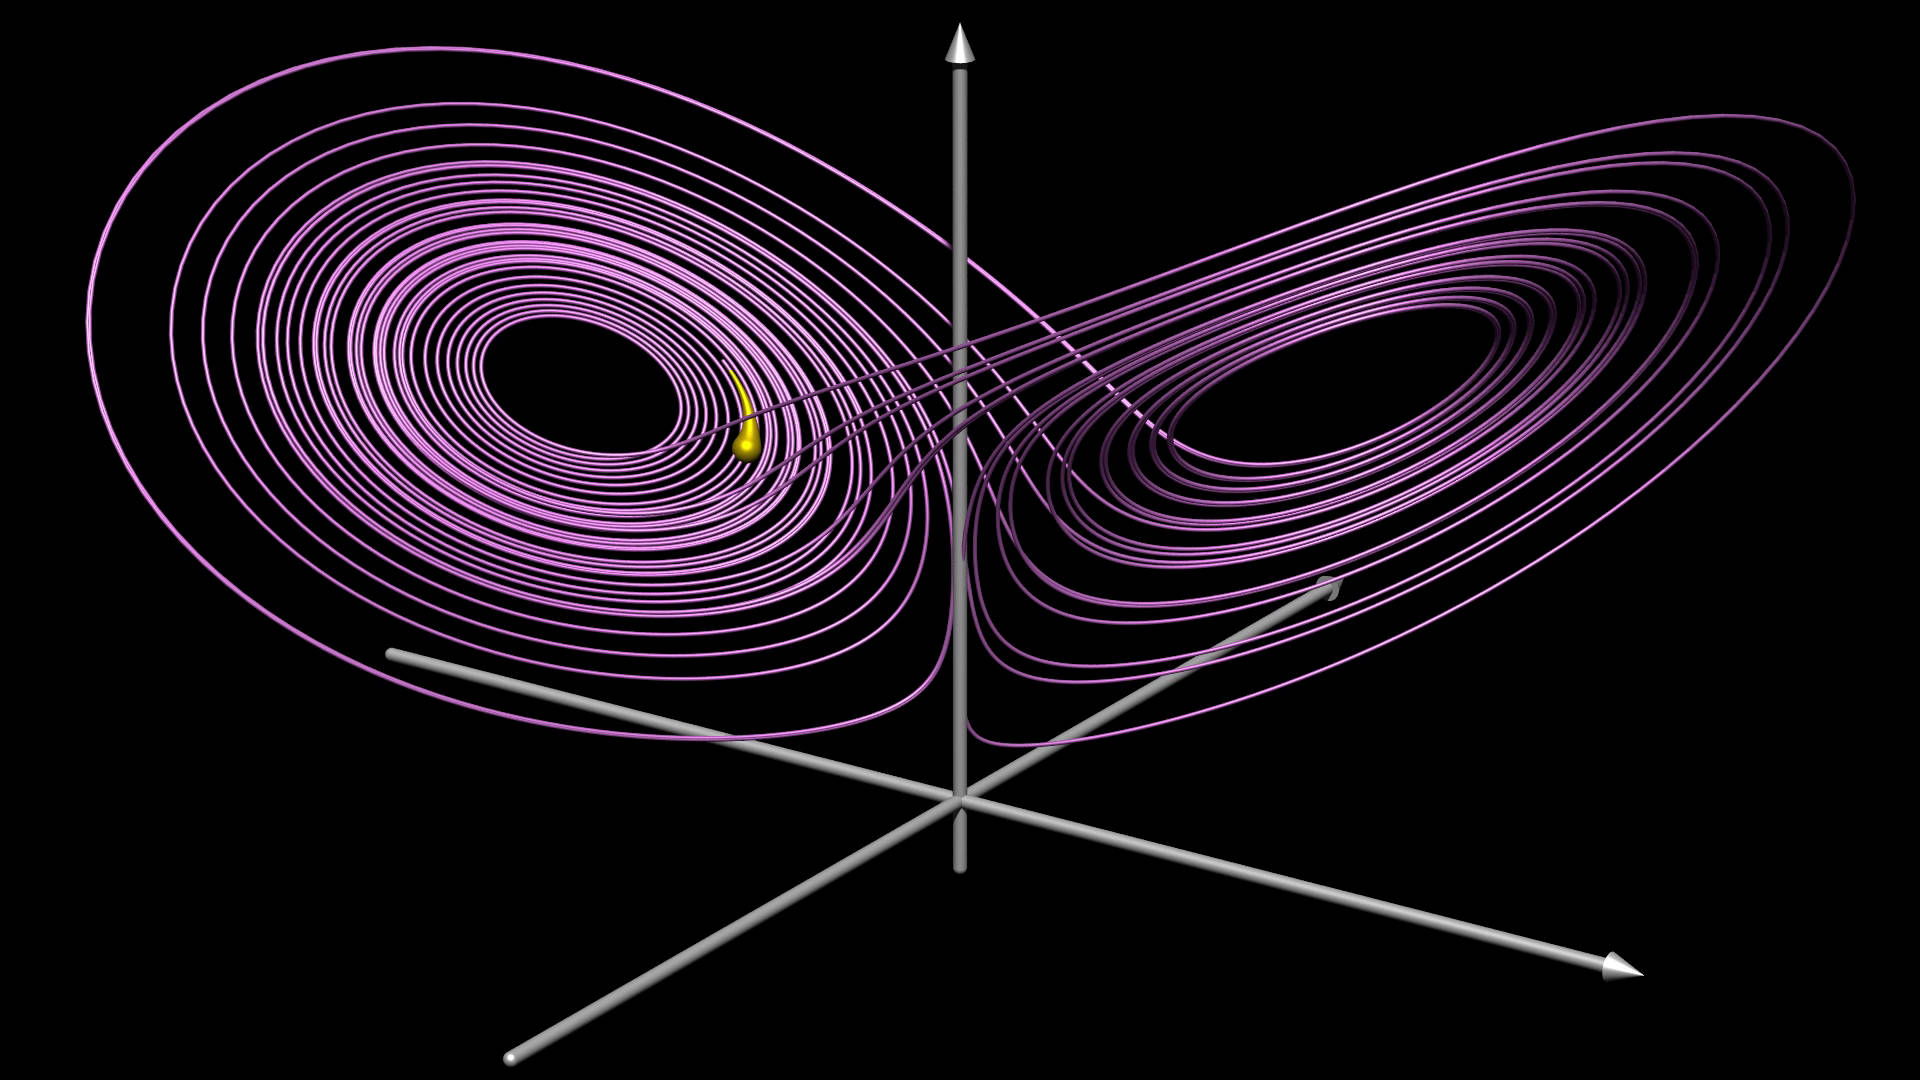
\includegraphics[width=.7\textwidth]{../images/lorenz_animation_thumbnail.jpg}
        \end{center}
    \end{frame}
    % Plots von ENSO. Lösungen konvergieren.
    % Idee: Plot wo unterwegs die Gleichung (Konstanten) ändert -> bleibt trotzdem auf einem ähnlichen Orbit
    % Link zum Sonnensystem herstellen!
    % Chaos in 3D möglich: Zeigen des Videos von Müller

\end{document}

